\documentclass[twoside,11pt]{article}

% ? Specify used packages
\usepackage[english]{babel}  %  For correct hyphenation rules
\usepackage{graphicx}        %  Use this one for final production.
% \usepackage[draft]{graphicx} %  Use this one for drafting.
% ? End of specify used packages

\pagestyle{headings}
\pagenumbering{roman}

% -----------------------------------------------------------------------------
% ? Document identification
% Fixed part
\newcommand{\stardoccategory}  {Starlink User Note}
\newcommand{\stardocinitials}  {SUN}
\newcommand{\stardocsource}    {sun\stardocnumber}

% Variable part - replace [xxx] as appropriate.
\newcommand{\stardocnumber}    {210.26}
\newcommand{\stardocauthors}   {R.F. Warren-Smith \& D.S. Berry}
\newcommand{\stardocdate}      {4th October 2011}
\newcommand{\stardoctitle}     {AST\\
                                A Library for Handling\\
                                World Coordinate Systems\\
                                in Astronomy}
\newcommand{\stardoccopyright} {Copyright (C) 2009 Science \& Technology Facilities Council}
\newcommand{\stardoctitlehtml} {AST - A Library for Handling World Coordinate
                                      Systems in Astronomy}
\newcommand{\stardocversion}   {V6.0}
\newcommand{\stardocmanual}    {Programmer's Guide\\(Fortran Version)}
\newcommand{\stardocmanualhtml}{Programmer's Guide (Fortran Version)}
\newcommand{\stardocabstract}  {
The AST library provides a comprehensive range of facilities for
attaching world coordinate systems to astronomical data, for
retrieving and interpreting that information in a variety of formats,
including FITS-WCS, and for generating graphical output based on it.

This programmer's manual should be of interest to anyone writing
astronomical applications which need to manipulate coordinate system
data, especially celestial or spectral coordinate systems. AST is portable and
environment-independent.
}
% ? End of document identification
% -----------------------------------------------------------------------------

% +
%  Name:
%     sun.tex
%
%  Purpose:
%     Template for Starlink User Note (SUN) documents.
%     Refer to SUN/199
%
%  Authors:
%     AJC: A.J.Chipperfield (Starlink, RAL)
%     BLY: M.J.Bly (Starlink, RAL)
%
%  History:
%     17-JAN-1996 (AJC):
%        Original with hypertext macros, based on MDL plain originals.
%     16-JUN-1997 (BLY):
%        Adapted for LaTeX2e.
%        Added picture commands.
%     {Add further history here}
%
% -

\newcommand{\stardocname}{\stardocinitials /\stardocnumber}
\markboth{\stardocname}{\stardocname}
\setlength{\textwidth}{160mm}
\setlength{\textheight}{230mm}
\setlength{\topmargin}{-2mm}
\setlength{\oddsidemargin}{0mm}
\setlength{\evensidemargin}{0mm}
\setlength{\parindent}{0mm}
\setlength{\parskip}{\medskipamount}
\setlength{\unitlength}{1mm}

% -----------------------------------------------------------------------------
%  Hypertext definitions.
%  ======================
%  These are used by the LaTeX2HTML translator in conjunction with star2html.

%  \htmlref{Comment}{Comment}.sty: version 2.0, 19 June 1992
%  Selectively in/exclude pieces of text.
%
%  Author
%    Victor Eijkhout                                      <eijkhout@cs.utk.edu>
%    Department of Computer Science
%    University Tennessee at Knoxville
%    104 Ayres Hall
%    Knoxville, TN 37996
%    USA

%  Do not remove the %begin{latexonly} and %end{latexonly} lines (used by
%  star2html to signify raw TeX that latex2html cannot process).
%begin{latexonly}
\makeatletter
\def\makeinnocent#1{\catcode`#1=12 }
\def\csarg#1#2{\expandafter#1\csname#2\endcsname}

\def\ThrowAwayComment#1{\begingroup
    \def\CurrentComment{#1}%
    \let\do\makeinnocent \dospecials
    \makeinnocent\^^L% and whatever other special cases
    \endlinechar`\^^M \catcode`\^^M=12 \xComment}
{\catcode`\^^M=12 \endlinechar=-1 %
 \gdef\xComment#1^^M{\def\test{#1}
      \csarg\ifx{PlainEnd\CurrentComment Test}\test
          \let\html@next\endgroup
      \else \csarg\ifx{LaLaEnd\CurrentComment Test}\test
            \edef\html@next{\endgroup\noexpand\end{\CurrentComment}}
      \else \let\html@next\xComment
      \fi \fi \html@next}
}
\makeatother

\def\includecomment
 #1{\expandafter\def\csname#1\endcsname{}%
    \expandafter\def\csname end#1\endcsname{}}
\def\excludecomment
 #1{\expandafter\def\csname#1\endcsname{\ThrowAwayComment{#1}}%
    {\escapechar=-1\relax
     \csarg\xdef{PlainEnd#1Test}{\string\\end#1}%
     \csarg\xdef{LaLaEnd#1Test}{\string\\end\string\{#1\string\}}%
    }}

%  Define environments that ignore their contents.
\excludecomment{comment}
\excludecomment{rawhtml}
\excludecomment{htmlonly}

%  Hypertext commands etc. This is a condensed version of the html.sty
%  file supplied with LaTeX2HTML by: Nikos Drakos <nikos@cbl.leeds.ac.uk> &
%  Jelle van Zeijl <jvzeijl@isou17.estec.esa.nl>. The LaTeX2HTML documentation
%  should be consulted about all commands (and the environments defined above)
%  except \xref and \xlabel which are Starlink specific.

\newcommand{\htmladdnormallinkfoot}[2]{#1\footnote{#2}}
\newcommand{\htmladdnormallink}[2]{#1}
\newcommand{\htmladdimg}[1]{}
\newenvironment{latexonly}{}{}
\newcommand{\hyperref}[4]{#2\ref{#4}#3}
\newcommand{\htmlref}[2]{#1}
\newcommand{\htmlimage}[1]{}
\newcommand{\htmladdtonavigation}[1]{}
\newcommand{\latexhtml}[2]{#1}
\newcommand{\html}[1]{}

%  Starlink cross-references and labels.
\newcommand{\xref}[3]{#1}
\newcommand{\xlabel}[1]{}

%  LaTeX2HTML symbol.
\newcommand{\latextohtml}{{\bf LaTeX}{2}{\tt{HTML}}}

%  Define command to re-centre underscore for Latex and leave as normal
%  for HTML (severe problems with \_ in tabbing environments and \_\_
%  generally otherwise).
\newcommand{\latex}[1]{#1}
\newcommand{\setunderscore}{\renewcommand{\_}{{\tt\symbol{95}}}}
\latex{\setunderscore}

%  Redefine the \tableofcontents command. This procrastination is necessary
%  to stop the automatic creation of a second table of contents page
%  by latex2html.
\newcommand{\latexonlytoc}[0]{\tableofcontents}

% -----------------------------------------------------------------------------
%  Debugging.
%  =========
%  Remove % on the following to debug links in the HTML version using Latex.

% \newcommand{\hotlink}[2]{\fbox{\begin{tabular}[t]{@{}c@{}}#1\\\hline{\footnotesize #2}\end{tabular}}}
% \renewcommand{\htmladdnormallinkfoot}[2]{\hotlink{#1}{#2}}
% \renewcommand{\htmladdnormallink}[2]{\hotlink{#1}{#2}}
% \renewcommand{\hyperref}[4]{\hotlink{#1}{\S\ref{#4}}}
% \renewcommand{\htmlref}[2]{\hotlink{#1}{\S\ref{#2}}}
% \renewcommand{\xref}[3]{\hotlink{#1}{#2 -- #3}}
%end{latexonly}
% -----------------------------------------------------------------------------
% ? Document specific \newcommand or \newenvironment commands.

\newcommand{\appref}[1]{Appendix~\ref{#1}}
\newcommand{\secref}[1]{\S\ref{#1}}
\begin{htmlonly}
   \newcommand{\appref}[1]{\ref{#1}}
   \newcommand{\secref}[1]{\ref{#1}}
\end{htmlonly}

\newcommand{\fitsurl}[0]{http://fits.gsfc.nasa.gov/}
\newcommand{\fitskey}[3]{{#1}&{#2}&{#3}\\}

% The following stuff has been moved out of the document body
% in an attempt to stop spurious behaviour form latex2html.

\begin{htmlonly}
  \newcommand{\latexonlytoc}[0]{}
\end{htmlonly}
\renewcommand{\thepage}{\arabic{page}}

% +
%  Name:
%     SST.TEX

%  Purpose:
%     Define LaTeX commands for laying out Starlink routine descriptions.

%  Language:
%     LaTeX

%  Type of Module:
%     LaTeX data file.

%  Description:
%     This file defines LaTeX commands which allow routine documentation
%     produced by the SST application PROLAT to be processed by LaTeX and
%     by LaTeX2html. The contents of this file should be included in the
%     source prior to any statements that make of the sst commands.

%  Notes:
%     The commands defined in the style file html.sty provided with LaTeX2html
%     are used. These should either be made available by using the appropriate
%     sun.tex (with hypertext extensions) or by putting the file html.sty
%     on your TEXINPUTS path (and including the name as part of the
%     documentstyle declaration).

%  Authors:
%     RFWS: R.F. Warren-Smith (STARLINK)
%     PDRAPER: P.W. Draper (Starlink - Durham University)

%  History:
%     10-SEP-1990 (RFWS):
%        Original version.
%     10-SEP-1990 (RFWS):
%        Added the implementation status section.
%     12-SEP-1990 (RFWS):
%        Added support for the usage section and adjusted various spacings.
%     8-DEC-1994 (PDRAPER):
%        Added support for simplified formatting using LaTeX2html.
%     {enter_further_changes_here}

%  Bugs:
%     {note_any_bugs_here}

% -

%  Define length variables.
\newlength{\sstbannerlength}
\newlength{\sstcaptionlength}
\newlength{\sstexampleslength}
\newlength{\sstexampleswidth}

%  Define a \tt font of the required size.
\latex{\newfont{\ssttt}{cmtt10 scaled1095}}
\html{\newcommand{\ssttt}{\tt}}

%  Define a command to produce a routine header, including its name,
%  a purpose description and the rest of the routine's documentation.
\newcommand{\sstlabel}[1]{}
\newcommand{\sstroutine}[3]{
   \goodbreak
   \rule{\textwidth}{0.5mm}
   \vspace{-7ex}
   \newline
   \settowidth{\sstbannerlength}{{\Large {\bf #1}}}
   \setlength{\sstcaptionlength}{\textwidth}
   \setlength{\sstexampleslength}{\textwidth}
   \addtolength{\sstbannerlength}{0.5em}
   \addtolength{\sstcaptionlength}{-2.0\sstbannerlength}
   \addtolength{\sstcaptionlength}{-5.0pt}
   \settowidth{\sstexampleswidth}{{\bf Examples:}}
   \addtolength{\sstexampleslength}{-\sstexampleswidth}
   \parbox[t]{\sstbannerlength}{\flushleft{\Large {\bf #1}}}
   \parbox[t]{\sstcaptionlength}{\center{\Large #2}}
   \parbox[t]{\sstbannerlength}{\flushright{\Large {\bf #1}}}
   \begin{description}
      #3
   \end{description}
}

%  Format the description section.
\newcommand{\sstdescription}[1]{\item[Description:] #1}

%  Format the usage section.
\newcommand{\sstusage}[1]{\item[Usage:] \mbox{} \\[1.3ex] {\ssttt #1}}

%  Format the invocation/synopsis section.
\newcommand{\sstinvocation}[1]{\item[Invocation:]\hspace{0.4em}{\tt #1}}
\newcommand{\sstsynopsis}[1]{\item[Synopsis:]\hspace{0.4em}{\tt #1}}

%  Format the attribute data type section.
\newcommand{\sstattributetype}[1]{
   \item[Type:] \mbox{} \\
      #1
}

%  Format the constructor section.
\newcommand{\sstconstructor}[1]{
   \item[Constructor Function:] \mbox{} \\
      #1
}

%  Format the arguments section.
\newcommand{\sstarguments}[1]{
   \item[Arguments:] \mbox{} \\
   \vspace{-3.5ex}
   \begin{description}
      #1
   \end{description}
}

%  Format the returned value section (for a function).
\newcommand{\sstreturnedvalue}[1]{
   \item[Returned Value:] \mbox{} \\
   \vspace{-3.5ex}
   \begin{description}
      #1
   \end{description}
}

%  Format the parameters section (for an application).
\newcommand{\sstparameters}[1]{
   \item[Parameters:] \mbox{} \\
   \vspace{-3.5ex}
   \begin{description}
      #1
   \end{description}
}

%  Format the applicability section.
\newcommand{\sstapplicability}[1]{
   \item[Clas\mbox{}s Applicability:] \mbox{} \\
   \vspace{-3.5ex}
   \begin{description}
      #1
   \end{description}
}

%  Format the examples section.
\newcommand{\sstexamples}[1]{
   \item[Examples:] \mbox{} \\
   \vspace{-3.5ex}
   \begin{description}
      #1
   \end{description}
}

%  Define the format of a subsection in a normal section.
\newcommand{\sstsubsection}[1]{ \item[{#1}] \mbox{} \\}

%  Define the format of a subsection in the examples section.
\newcommand{\sstexamplesubsection}[2]{\sloppy
\item[\parbox{\sstexampleslength}{\ssttt #1}] \mbox{} \\ #2 }

%  Format the notes section.
\newcommand{\sstnotes}[1]{\item[Notes:] \mbox{} \\[1.3ex] #1}

%  Provide a general-purpose format for additional (DIY) sections.
\newcommand{\sstdiytopic}[2]{\item[{\hspace{-0.35em}#1\hspace{-0.35em}:}] \mbox{} \\[1.3ex] #2}

%  Format the a generic section as a list
\newcommand{\sstdiylist}[2]{
   \item[#1:] \mbox{} \\
   \vspace{-3.5ex}
   \begin{description}
      #2
   \end{description}
}

%  Format the implementation status section.
\newcommand{\sstimplementationstatus}[1]{
   \item[{Implementation Status:}] \mbox{} \\[1.3ex] #1}

%  Format the bugs section.
\newcommand{\sstbugs}[1]{\item[Bugs:] #1}

%  Format a list of items while in paragraph mode.
\newcommand{\sstitemlist}[1]{
  \mbox{} \\
  \vspace{-3.5ex}
  \begin{itemize}
     #1
  \end{itemize}
}

%  Define the format of an item.
\newcommand{\sstitem}{\item}

%  Now define html equivalents of those already set. These are used by
%  latex2html and are defined in the html.sty files.
\begin{htmlonly}

%  Re-define \ssttt.
   \newcommand{\ssttt}{\tt}

%  sstroutine.
%   \newcommand{\sstroutine}[3]{
%      \subsection{#1\xlabel{#1}-\label{#1}#2}
%      \begin{description}
%         #3
%      \end{description}
%   }
   \newcommand{\sstlabel}[1]{\label{#1}\xlabel{#1}}
   \newcommand{\sstroutine}[3]{
      \subsection{#1 - #2}
      \begin{description}
         #3
      \end{description}
   }

%  sstdescription
   \newcommand{\sstdescription}[1]{\item[Description:]
      \begin{description}
         #1
      \end{description}
   }

%  sstusage
   \newcommand{\sstusage}[1]{\item[Usage:]
      \begin{description}
         {\ssttt #1}
      \end{description}
   }

%  sstinvocation
   \newcommand{\sstinvocation}[1]{\item[Invocation:]
      \begin{description}
         {\ssttt #1}
      \end{description}
   }

%  sstsynopsis
   \newcommand{\sstsynopsis}[1]{\item[Synopsis:]
      \begin{description}
         {\ssttt #1}
      \end{description}
   }

%  sstattributetype
   \newcommand{\sstattributetype}[1]{\item[Type:]
         #1
   }

%  sstconstructor
   \newcommand{\sstconstructor}[1]{\item[Constructor Function:]
         #1
   }

%  sstarguments
   \newcommand{\sstarguments}[1]{
      \item[Arguments:]
      \begin{description}
         #1
      \end{description}
   }

%  sstreturnedvalue
   \newcommand{\sstreturnedvalue}[1]{
      \item[Returned Value:]
      \begin{description}
         #1
      \end{description}
   }

%  sstparameters
   \newcommand{\sstparameters}[1]{
      \item[Parameters:]
      \begin{description}
         #1
      \end{description}
   }

%  sstapplicability
   \newcommand{\sstapplicability}[1]{
      \item[Clas\mbox{}s Applicability:]
      \begin{description}
         #1
      \end{description}
   }

%  sstexamples
   \newcommand{\sstexamples}[1]{
      \item[Examples:]
      \begin{description}
         #1
      \end{description}
   }

%  sstsubsection
   \newcommand{\sstsubsection}[1]{\item[{#1}]}

%  sstexamplesubsection
   \newcommand{\sstexamplesubsection}[2]{\item[{\ssttt #1}] \\ #2}

%  sstnotes
   \newcommand{\sstnotes}[1]{\item[Notes:]
      \begin{description}
         #1
      \end{description}
   }

%  sstdiytopic
   \newcommand{\sstdiytopic}[2]{\item[{#1}]
      \begin{description}
         #2
      \end{description}
   }

%  sstimplementationstatus
   \newcommand{\sstimplementationstatus}[1]{\item[Implementation Status:]
      \begin{description}
         #1
      \end{description}
   }

%  sstitemlist
   \newcommand{\sstitemlist}[1]{
      \begin{itemize}
         #1
      \end{itemize}
   }
\end{htmlonly}

%  End of "sst.tex" layout definitions.
% .
% @(#)sst.tex   1.4   95/06/06 11:46:41   96/07/05 10:28:17





% ? End of document specific commands
% -----------------------------------------------------------------------------
%  \htmlref{Title}{Title} Page.
%  ===========
\renewcommand{\thepage}{\roman{page}}
\begin{document}
\thispagestyle{empty}

%  Latex document header.
%  ======================
\begin{latexonly}
   CCLRC / {\sc Rutherford Appleton Laboratory} \hfill {\bf \stardocname}\\
   {\large Particle Physics \& Astronomy Research Council}\\
   {\large Starlink Project\\}
   {\large \stardoccategory\ \stardocnumber}
   \begin{flushright}
   \stardocauthors\\
   \stardocdate
   \end{flushright}
   \vspace{-4mm}
   \rule{\textwidth}{0.5mm}
   \vspace{-7mm}
   \begin{center}
   {\Huge\bf  \stardoctitle \\ [2.0ex]}
   {\LARGE\bf \stardocversion \\ [1.0ex]}
   {\Huge\bf  \stardocmanual}
   \end{center}

% ? Add picture here if required for the LaTeX version.
   \begin{center}
   \mbox{}\hfill
   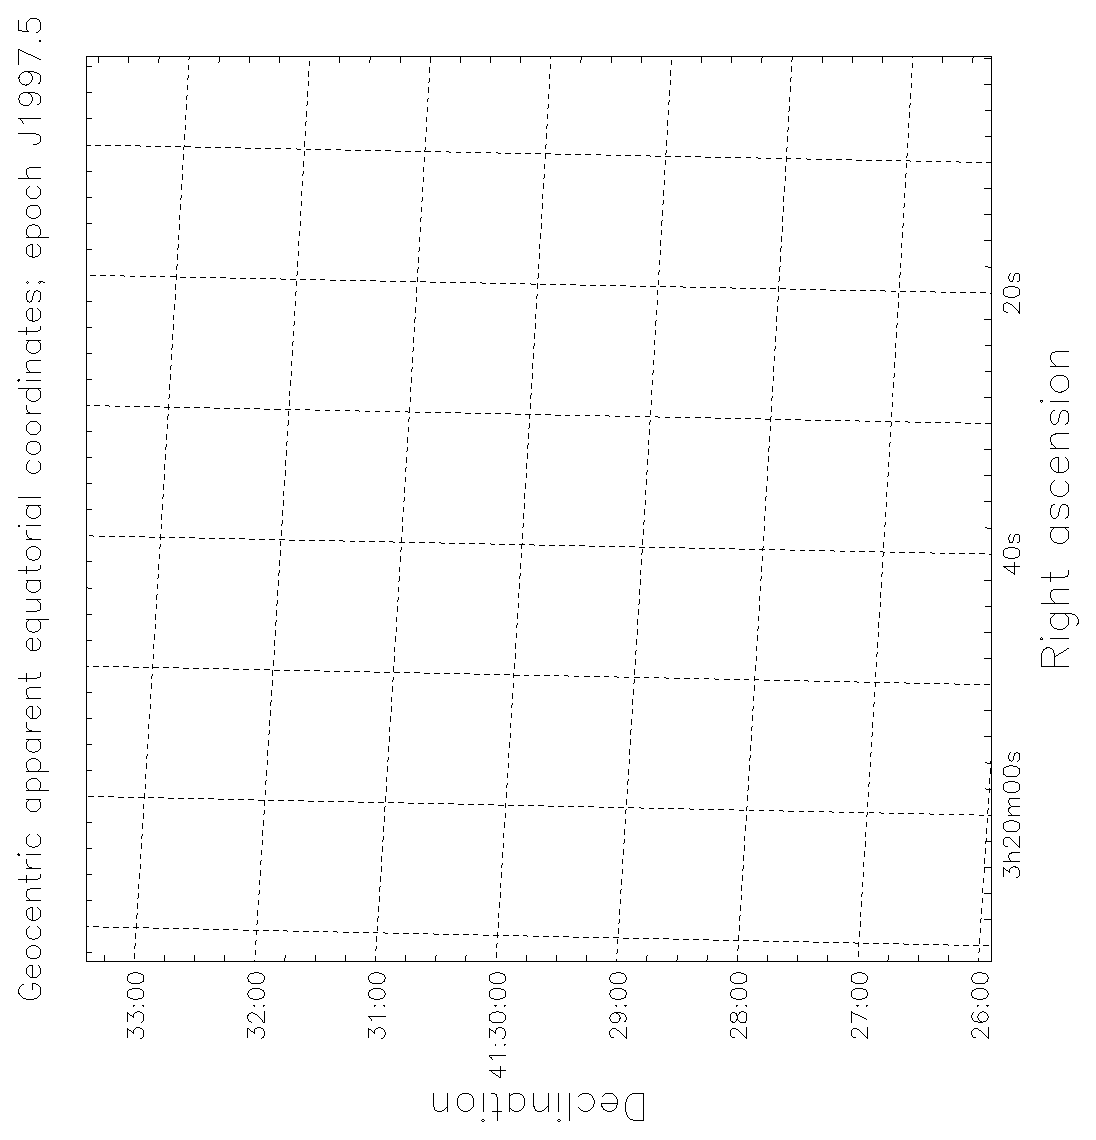
\includegraphics[scale=0.25,angle=-90]{sun210_figures/fronta_bw.eps}\hfill
   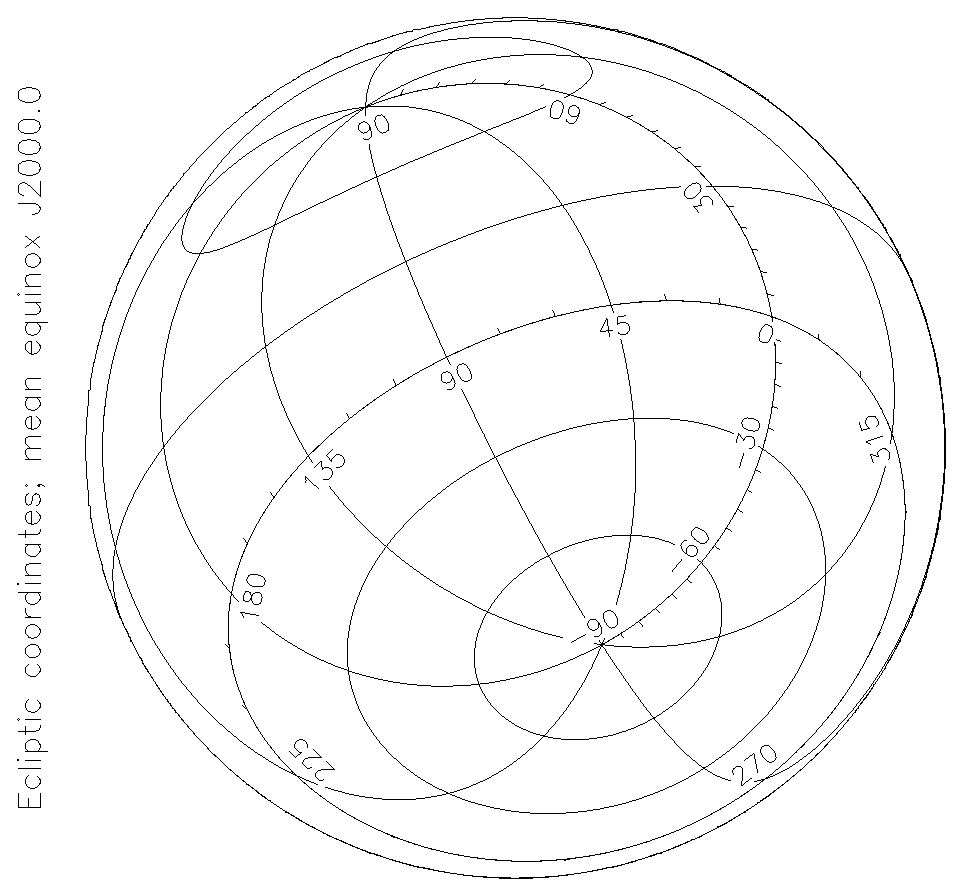
\includegraphics[scale=0.25,angle=-90]{sun210_figures/frontb_bw.eps}\hfill
   \includegraphics[scale=0.25,angle=-90]{sun210_figures/frontc_bw.eps}\hfill
   \mbox{}
   \end{center}
% ? End of picture

% ? Heading for abstract if used.
   \begin{center}
      {\Large\bf Abstract}
   \end{center}
% ? End of heading for abstract.
\end{latexonly}

%  HTML documentation header.
%  ==========================
\begin{htmlonly}
   \xlabel{}
   \begin{rawhtml} <H1> \end{rawhtml}
      \stardoctitlehtml
   \begin{rawhtml} </H1> \end{rawhtml}

% ? Add picture here if required for the hypertext version.
   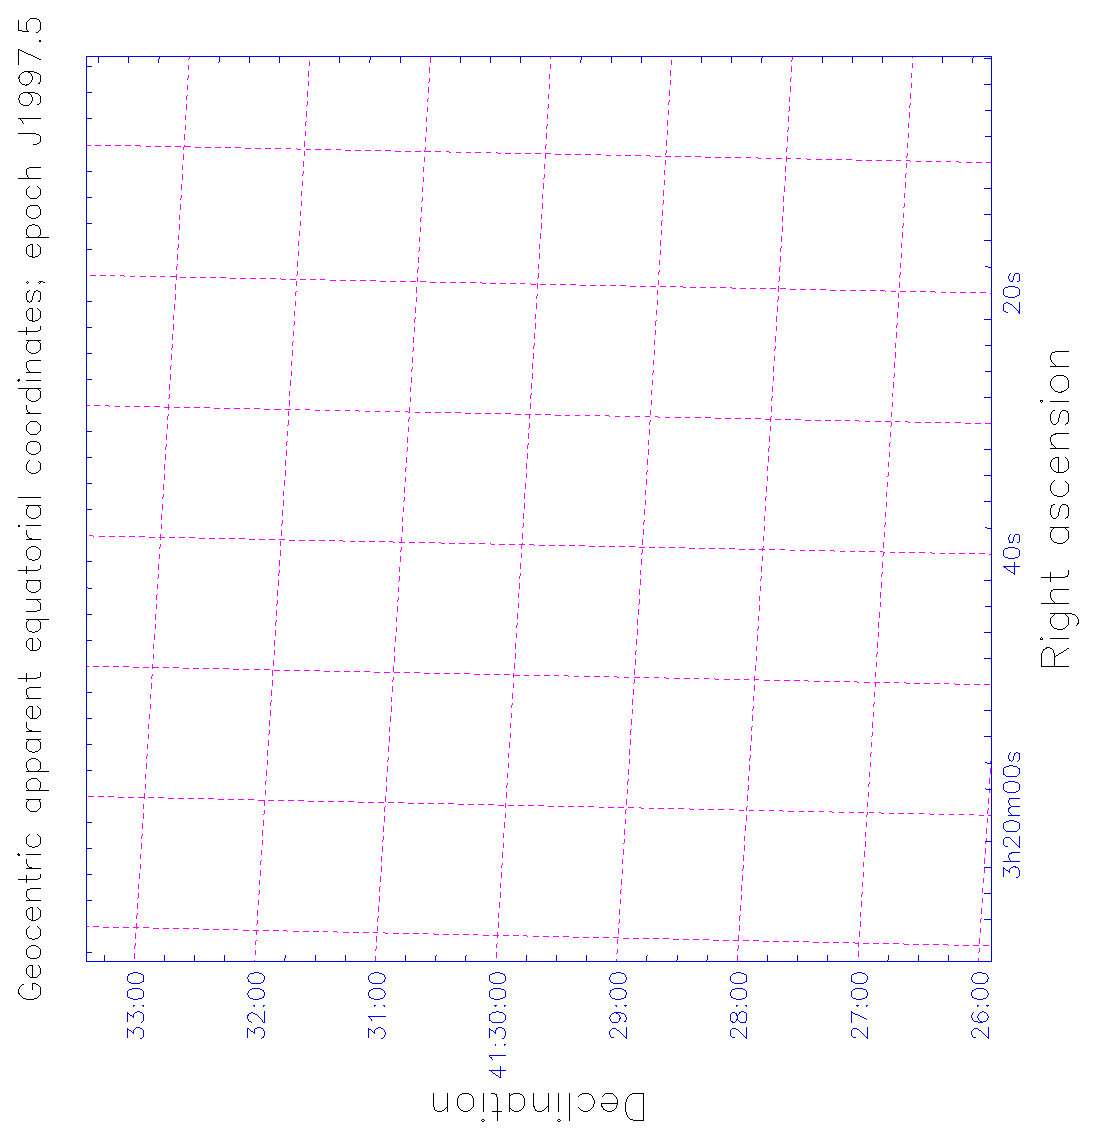
\includegraphics[scale=0.3,angle=-90]{sun210_figures/fronta.eps}\hfill
   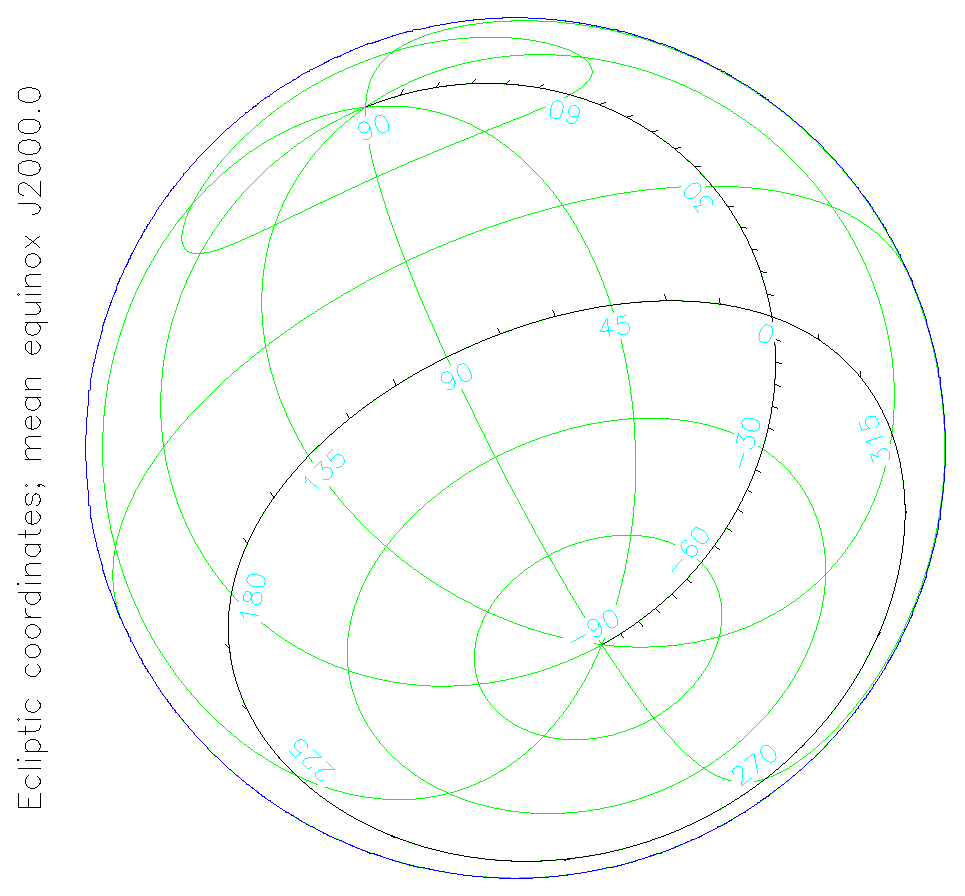
\includegraphics[scale=0.3,angle=-90]{sun210_figures/frontb.eps}\hfill
   \includegraphics[scale=0.3,angle=-90]{sun210_figures/frontc.eps}
% ? End of picture

   \begin{rawhtml} <H1> \end{rawhtml}
      \stardocversion
      \stardocmanualhtml
   \begin{rawhtml} </H1> \end{rawhtml}
   \begin{rawhtml} <P> <I> \end{rawhtml}
   \stardoccategory\ \stardocnumber \\
   \stardocauthors \\
   \stardocdate
   \begin{rawhtml} </I> </P> \end{rawhtml}
   \begin{rawhtml} <P> <I> \end{rawhtml}
   (For the C version of this document, please see \xref{SUN/211}{sun211}{}.)
   \begin{rawhtml} </I> </P> \end{rawhtml}
   \begin{rawhtml} <H3> \end{rawhtml}
      \htmladdnormallink{CCLRC}{http://www.cclrc.ac.uk} /
      \htmladdnormallink{Rutherford Appleton Laboratory}
                        {http://www.cclrc.ac.uk/ral} \\
      \htmladdnormallink{Particle Physics \& Astronomy Research Council}
                        {http://www.pparc.ac.uk} \\
   \begin{rawhtml} </H3> <H2> \end{rawhtml}
      \htmladdnormallink{Starlink Project}{http://www.starlink.ac.uk/}
   \begin{rawhtml} </H2> \end{rawhtml}
   \htmladdnormallink{\htmladdimg{source.gif} Retrieve hardcopy}
      {http://www.starlink.ac.uk/cgi-bin/hcserver?\stardocsource}\\

%  HTML document table of contents.
%  ================================
%  Add table of contents header and a navigation button to return to this
%  point in the document (this should always go before the abstract \section).
  \label{stardoccontents}
  \begin{rawhtml}
    <HR>
    <H2>Contents</H2>
  \end{rawhtml}
  \htmladdtonavigation{\htmlref{\htmladdimg{contents_motif.gif}}
        {stardoccontents}}

% ? New section for abstract if used.
  \section{\xlabel{abstract}Abstract}
% ? End of new section for abstract
\end{htmlonly}

% -----------------------------------------------------------------------------
% ? Document Abstract. (if used)
%  ==================
\stardocabstract
% ? End of document abstract
% -----------------------------------------------------------------------------
% ? Document Copyright Statement.
%  =============================
   \begin{latexonly}
      \newpage
      \vspace*{\fill}
      \stardoccopyright
   \end{latexonly}
% ? End of Document Copyright Statement.
% -----------------------------------------------------------------------------
% ? Latex document \htmlref{Table}{Table} of Contents (if used).
%  ===========================================
  \cleardoublepage
  \cleardoublepage
  \begin{latexonly}
    \setlength{\parskip}{0mm}
    \latexonlytoc
    \setlength{\parskip}{\medskipamount}
    \markboth{\stardocname}{\stardocname}
  \end{latexonly}
% ? End of Latex document table of contents
% -----------------------------------------------------------------------------
\cleardoublepage
\setcounter{page}{1}

\null\vspace {5mm}
\begin{latexonly}
   \begin {center}
   \rule{80mm}{0.5mm} \\ [1ex]
   {\Large\bf \stardoctitle \\ [2.5ex]
              \stardocversion} \\ [2ex]
   \rule{80mm}{0.5mm}

   \vspace{10mm}
   {\em{This is the Fortran version of this document.\\
        For the C version, please see SUN/211.}}
   \end{center}
\end{latexonly}

% Main text of document.
\vspace{7mm}
\pagenumbering{arabic}
\section{Introduction}

Welcome to the AST library. If you are writing software for astronomy
and need to use celestial coordinates ({\em{e.g.}}\ RA and Dec), spectral
coordinates ({\em{e.g.}}\ wavelength, frequency, {\em{etc.}}), or
other coordinate system information, then this library should be of
interest. It provides solutions for most of the problems you will meet
and allows you to write robust and flexible software. It is able to read
and write WCS information in a variety of formats, including
\htmladdnormallink{FITS-WCS}{http://fits.gsfc.nasa.gov/fits_wcs.html}.

%\subsection{TBW---What is a World Coordinate \htmlref{System}{System}?}

\subsection{What Problems Does AST Tackle?}

Here are some of the main problems you may face when handling world
coordinate system (WCS) information and the solutions that AST
provides:

\begin{description}
\item[1. The Variety of Coordinate Systems]\mbox{}\\
Astronomers use a wide range of differing coordinate systems to describe
positions within a variety of physical domains. For instance, there are a
large number of celestial coordinate systems in use within astronomy to
describe positions on the sky. Understanding these, and knowing how to
convert coordinates between them, can require considerable expertise. It
can also be difficult to decide which of them your software should support.
The same applies to coordinate systems describing other domains, such as
position within an electro-magnetic spectrum.

{\bf{Solution.}} AST has built-in knowledge of many coordinate systems
and allows you to convert freely between them without specialist
knowledge. This avoids the need to embed details of specific
coordinate systems in your software. You also benefit automatically
when new coordinate systems are added to AST.

\item[2. Storing and Retrieving WCS Information]\mbox{}\\
Storing coordinate system information in astronomical datasets and
retrieving it later can present a considerable challenge. Typically,
it requires knowledge of rather complex conventions
({\em{e.g.}}\ FITS) which are low-level, often mis-interpreted and may
be subject to change. Exchanging information with other software
systems is further complicated by the number of different conventions
in use.

{\bf{Solution.}} AST combines a unifying high-level description of WCS
information with the ability to save and restore this using a variety
of formats. Details of the formats, which include FITS, are handled
internally by AST. This frees you from the need to understand them or
embed the details in your software. Again, you benefit automatically
when new formats are added to AST.

\item[3. Generating Graphical Output]\mbox{}\\
Producing graphical displays involving curvilinear coordinate systems,
such as celestial coordinate grids, can be complicated. Particular
difficulties arise when handling large areas of sky, the polar regions
and discontinuous ({\em{e.g.}}\ segmented) sky projections.  Even just
numbering and labelling curvilinear axes is rarely straightforward.

{\bf{Solution.}} AST provides plotting facilities especially designed
for use with curvilinear coordinate systems. These include the
plotting of axes and complete labelled coordinate grids.  A large
number of options are provided for tailoring the output to your
specific needs.

\item[4. Aligning Data from Different Sources]\mbox{}\\
One of the main uses of coordinate systems is to facilitate the
inter-comparison of data from different sources. A typical use might
be to plot (say) radio contours over an optical image.  In practice,
however, different celestial coordinate systems may have been used,
making accurate alignment far from simple.

{\bf{Solution}} AST provides a one-step method of aligning datasets,
searching for all possible intermediate coordinate systems.  This
makes it simple to directly inter-relate the pixel coordinates of
different datasets.

\item[5. Handling Different Types of Coordinate \htmlref{System}{System}]\mbox{}\\
Not all coordinate systems used in astronomy are celestial ones, so if
you are writing general-purpose software such as (say) a display tool,
you may also need to handle axes representing wavelength, distance,
time or whatever else comes along. Obviously, you would prefer not to
handle each one as a special case.

{\bf{Solution}} AST uses the same flexible high-level model to
describe all types of coordinate system. This allows you to write
software that handles different kinds of coordinate axis without
introducing special cases.
\end{description}

\subsection{Other Design Objectives}

As well as its scientific objectives, the AST library's design
includes a number of technical criteria intended to make it applicable
to as wide a range of projects as possible. The main considerations
are described here:

\begin{enumerate}
\item {\bf{Minimum Software Dependencies.}}
The AST library depends on no other other software\footnote{It now comes with a
minimal cut-down version of the widely-available SLALIB positional astronomy
library (\xref{SUN/67}{sun67}{}), including just those functions needed
by AST, and the previous dependency on SLALIB is no longer present}.

\item {\bf{Environment Independence.}}
AST is designed so that it can operate in a variety of ``programming
environments'' and is not tied to any particular one. To allow this,
it uses simple, flexible interfaces to obtain the following services:

\begin{itemize}
\item {\bf{Data Storage.}} Data I/O operations are based on text
and/or FITS headers. This makes it easy to interface to a wide variety
of astronomical data formats in a machine-independent way.

\item {\bf{Graphics.}} Graphical output is produced {\em{via}} a
simple generic graphics interface, which may easily be re-implemented
over different graphics systems. AST provides a default implementation
based on the widely-used PGPLOT graphics system
(\xref{SUN/15}{sun15}{}).

\item {\bf{Error Handling.}} Error messages are written to standard
error by default, but go through a simple generic interface similar to
that used for graphics (above). This permits error message delivery
{\em{via}} other routes when necessary ({\em{e.g.}} in a graphical
interface).
\end{itemize}

\item {\bf{Multiple Language Support.}}
AST has been designed to be called from more than one language.
Both Fortran and C interfaces are available (see
\xref{SUN/211}{sun211}{} for the C version)
and use from C$++$ is also straightforward if the C interface is
included using:

\begin{quote}
\small
\begin{verbatim}
extern "C" {
#include "ast.h"
}
\end{verbatim}
\normalsize
\end{quote}

A JNI interface (known as ``JNIAST'' - see
\htmladdnormallink{http://www.starlink.ac.uk/jniast/}
{http://www.starlink.ac.uk/jniast/}) has also been developed by Starlink
which allows AST to be used from Java.

\item {\bf{\htmlref{Object}{Object} Oriented Design.}}
AST uses ``object oriented'' techniques internally in order to provide
a flexible and easily-extended programming model.  A fairly
traditional calling interface is provided, however, so that the
library's facilities are easily accessible to programmers using
Fortran and C.

\item {\bf{Portability.}}
AST is implemented entirely in ANSI standard C and, when called
{\em{via}} its C interface, makes no explicit use of any
machine-dependent facilities.

The Fortran interface is, unavoidably, machine dependent. However, the
potential for problems has been minimised by encapsulating the
interface layer in a compact set of C macros which facilitate its
transfer to other platforms. No Fortran compiler is needed to build
the library.

Currently, AST is supported by Starlink on PC~Linux, Sun~Solaris and
Tru64~Unix (formerly DEC~UNIX) platforms.
\end{enumerate}

\subsection{What Does ``AST'' Stand For?}

The library name ``AST'' stands for ``ASTrometry Library''. The name
arose when it was thought that knowledge of ``astrometry''
({\em{i.e.}}\ celestial coordinate systems) would form the bulk of the
library.  In fact, it turns out that astrometry forms only a minor
component, but the name AST has stuck.

\cleardoublepage
\section{Overview of AST Concepts}

This section presents a brief overview of AST concepts. It is intended
as a basic orientation course before you move on to the more technical
considerations in subsequent sections.

\subsection{\label{ss:mappingoverview}Relationships Between Coordinate Systems}

The relationships between coordinate systems are represented in AST by
Objects called Mappings. A \htmlref{Mapping}{Mapping} does not represent a coordinate
system itself, but merely the process by which you move from one
coordinate system to another related one.

\begin{latexonly}
   A convenient picture of a Mapping is as a ``black box''
   (Figure~\ref{fig:mapping}) into which you can feed sets of
   coordinates.
   \begin{figure}[bhtp]
   \begin{center}
   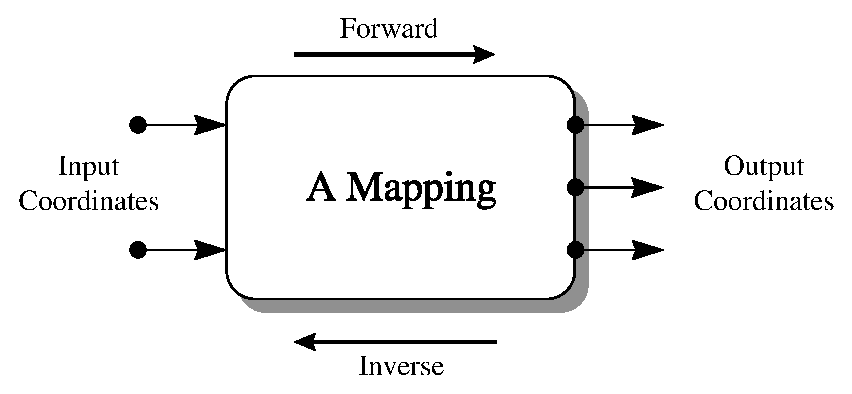
\includegraphics[scale=0.7]{sun210_figures/mapping.eps}
   \caption{A Mapping viewed as a ``black box'' for transforming coordinates.}
   \label{fig:mapping}
   \end{center}
   \end{figure}
\end{latexonly}
\begin{htmlonly}
   A convenient picture of a Mapping is as a ``black box'' (see Figure
   below) into which you can feed sets of coordinates.
   \begin{quote}
   \begin{figure}[bhtp]
   \label{fig:mapping}
   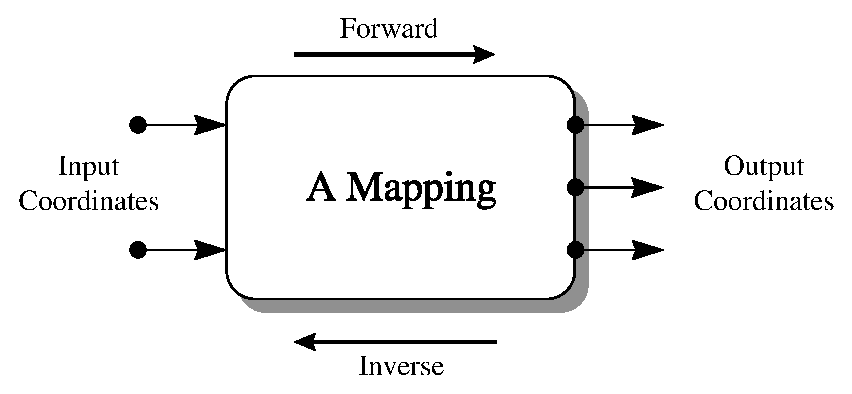
\includegraphics[scale=1.2]{sun210_figures/mapping.eps}
   \caption{A Mapping viewed as a ``black box'' for transforming coordinates.}
   \end{figure}
   \end{quote}
\end{htmlonly}
For each set you feed in, the Mapping returns a corresponding set of
transformed coordinates. Since each set of coordinates represents a
point in a coordinate space, the Mapping acts to inter-relate
corresponding positions in the two spaces, although what these spaces
represent is unspecified.  Notice that a Mapping need not have the
same number of input and output coordinates. That is, the two
coordinate spaces which it inter-relates need not have the same number
of dimensions.

In many cases, the transformation can, in principle, be performed in
either direction: either from the {\em{input}} coordinate space to the
{\em{output,}} or {\em{vice versa.}} The first of these is termed the
{\em{forward}} transformation and the other the {\em{inverse}}
transformation.


{\bf{Further reading:}} For a more complete discussion of Mappings,
see~\secref{ss:mappings}.

\subsection{\label{ss:mappingselection}Mappings Available}

The basic concept of a \htmlref{Mapping}{Mapping} (\secref{ss:mappingoverview}) is rather
generic and obviously it is necessary to have specific Mappings that
implement specific relationships between coordinate systems. AST
provides a range of these, to perform transformations such as the
following and, where appropriate, their inverses:

\begin{itemize}
\item Conversions between various celestial coordinate systems (the
\htmlref{SlaMap}{SlaMap}).

\item Conversions between various spectral coordinate systems (the
\htmlref{SpecMap}{SpecMap} and \htmlref{GrismMap}{GrismMap}).

\item Conversions between various time systems (the \htmlref{TimeMap}{TimeMap}).

\item Conversion between 2-dimensional spherical celestial coordinates
(longitude and latitude) and a 3-dimensional vectorial positions (the \htmlref{SphMap}{SphMap}).

\item Various projections of the celestial sphere on to 2-dimensional
coordinate spaces---{\em{i.e.}}\ map projections (the \htmlref{DssMap}{DssMap} and \htmlref{WcsMap}{WcsMap}).

\item Permutation, introduction and elimination of coordinates (the
\htmlref{PermMap}{PermMap}).

\item Various linear coordinate transformations (the \htmlref{MatrixMap}{MatrixMap}, \htmlref{WinMap}{WinMap},
\htmlref{ShiftMap}{ShiftMap} and \htmlref{ZoomMap}{ZoomMap}).

\item General N-dimensional polynomial transformations (the \htmlref{PolyMap}{PolyMap}).

\item Lookup tables (the \htmlref{LutMap}{LutMap}).

\item General-purpose transformations expressed using arithmetic
operations and functions similar to those available in Fortran (the
\htmlref{MathMap}{MathMap}).

\item Transformations for internal use within a program, based on
private transformation routines which you write yourself in Fortran
(the \htmlref{IntraMap}{IntraMap}).
\end{itemize}

{\bf{Further reading:}} For a more complete description of each of the
Mappings mentioned above, see its entry in
\appref{ss:classdescriptions}. In addition, see the discussion of the
PermMap in \secref{ss:permmapexample}, the \htmlref{UnitMap}{UnitMap} in
\secref{ss:unitmapexample} and the IntraMap in
\secref{ss:intramaps}. The ZoomMap is used as an example throughout
\secref{ss:primer}.

\subsection{\label{ss:cmpmapoverview}Compound Mappings}

The Mappings described in \secref{ss:mappingselection} provide a set
of basic building blocks from which more complex Mappings may be
constructed. The key to doing this is a type of \htmlref{Mapping}{Mapping} called a
\htmlref{CmpMap}{CmpMap}, or compound Mapping.  A CmpMap's role is, in principle, very
simple: it allows any other pair of Mappings to be joined together
into a single entity which behaves as if it were a single Mapping. A
CmpMap is therefore a container for another pair of Mappings.

\begin{latexonly}
   A pair of Mappings may be combined using a CmpMap in either of two
   ways. The first of these, {\em{in series,}} is illustrated in
   Figure~\ref{fig:seriescmpmap}.
   \begin{figure}
   \begin{center}
   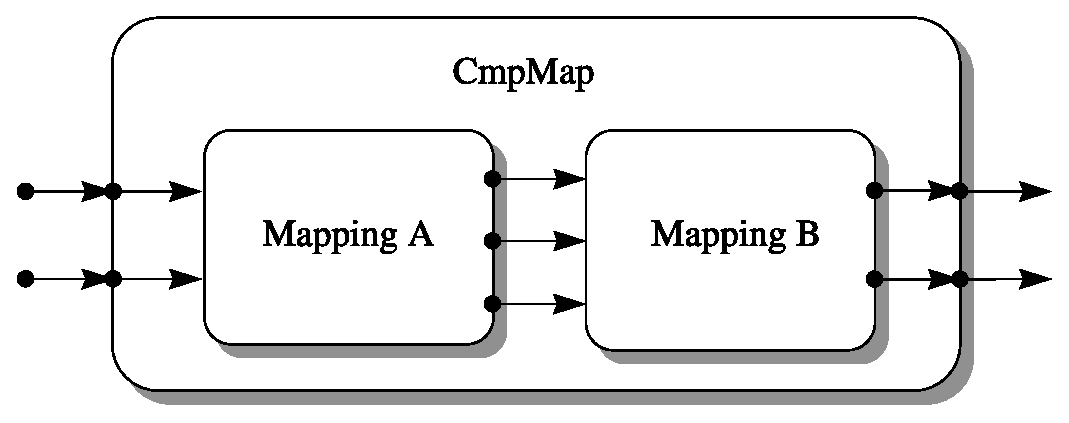
\includegraphics[scale=0.5]{sun210_figures/series.eps}
   \caption{A CmpMap (compound Mapping) composed of two component
   Mappings joined in series. The output coordinates of the first Mapping
   feed into the input coordinates of the second one, so that the whole
   entity behaves like a single Mapping.}
   \label{fig:seriescmpmap}
   \end{center}
   \end{figure}
\end{latexonly}
\begin{htmlonly}
   A pair of Mappings may be combined using a CmpMap in either of two
   ways. The first of these, {\em{in series,}} is illustrated in the
   following Figure.
   \begin{quote}
   \begin{figure}
   \label{fig:seriescmpmap}
   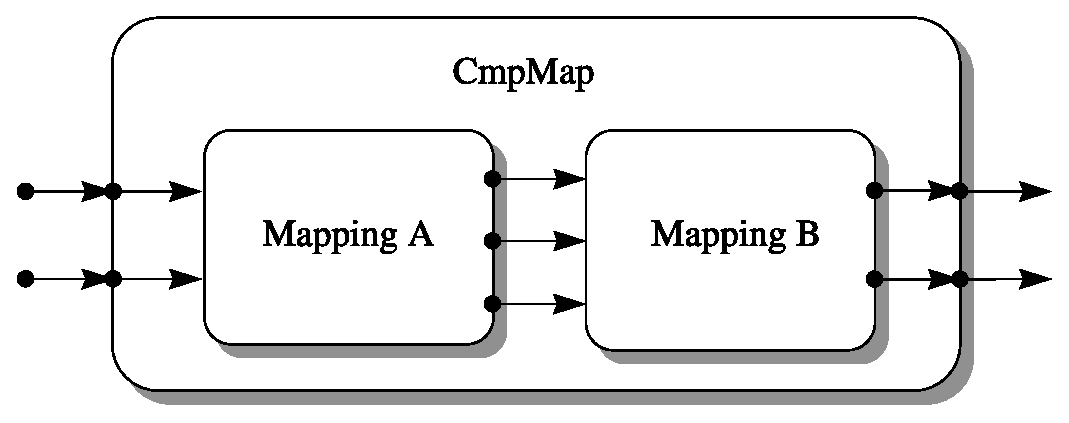
\includegraphics[scale=1.0]{sun210_figures/series.eps}
   \caption{A CmpMap (compound Mapping) composed of two component
   Mappings joined in series. The output coordinates of the first Mapping
   feed into the input coordinates of the second one, so that the whole
   entity behaves like a single Mapping.}
   \end{figure}
   \end{quote}
\end{htmlonly}
\begin{latexonly}
   Here, the transformations implemented by each component Mapping are
   performed one after the other, with the output from the first Mapping
   feeding into the second.  The second way, {\em{in parallel,}} is shown in
   Figure~\ref{fig:parallelcmpmap}.
   \begin{figure}
   \begin{center}
   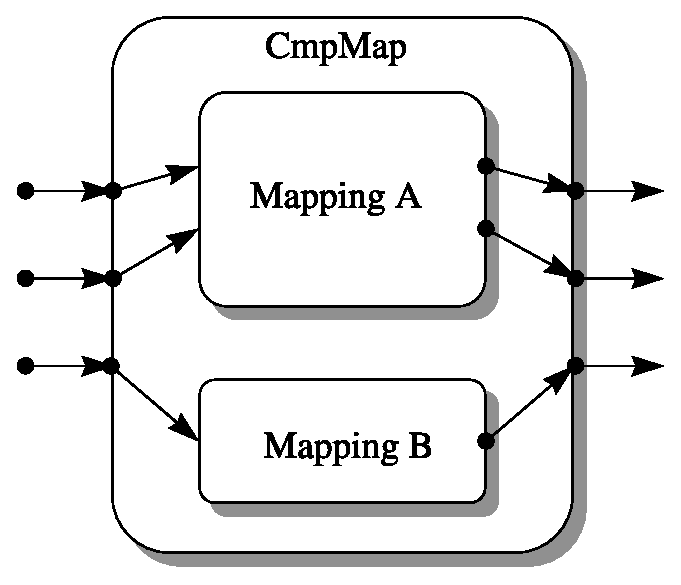
\includegraphics[scale=0.75]{sun210_figures/parallel.eps}
   \caption{A CmpMap composed of two Mappings joined in parallel. Each
   component Mapping acts on a complementary subset of the input and
   output coordinates.}
   \label{fig:parallelcmpmap}
   \end{center}
   \end{figure}
\end{latexonly}
\begin{htmlonly}
   Here, the transformations implemented by each component Mapping are
   performed one after the other, with the output from the first Mapping
   feeding into the second.  The second way, {\em{in parallel,}} is shown in
   the Figure below.
   \begin{quote}
   \begin{figure}
   \label{fig:parallelcmpmap}
   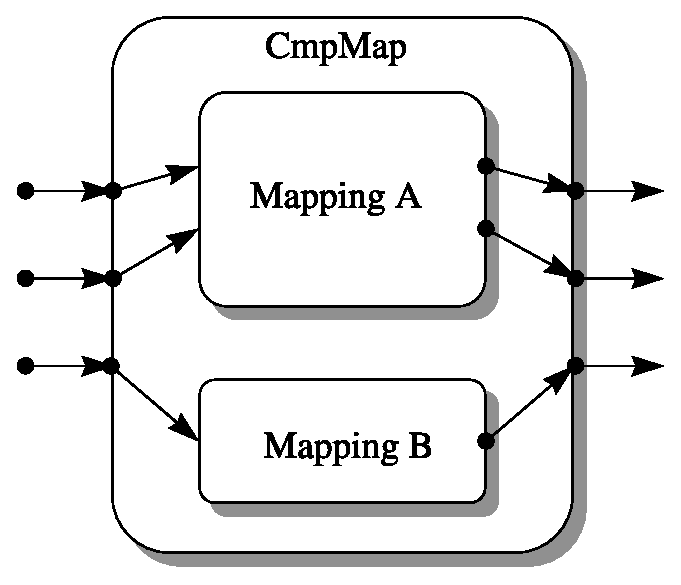
\includegraphics[scale=1.0]{sun210_figures/parallel.eps}
   \caption{A CmpMap composed of two Mappings joined in parallel. Each
   component Mapping acts on a complementary subset of the input and
   output coordinates.}
   \end{figure}
   \end{quote}
\end{htmlonly}
In this case, each Mapping acts on a complementary subset of the
input and output coordinates.\footnote{A pair of Mappings can be combined
in a third way using a \htmlref{TranMap}{TranMap}. A TranMap allows the forward
transformation of one Mapping to be combined with the inverse
transformation of another to produce a single Mapping.}

\begin{latexonly}
   The CmpMap forms the key to building arbitrarily complex Mappings
   because it is itself a form of Mapping. This means that a CmpMap may
   contain other CmpMaps as components
   ({\em{e.g.}}\ Figure~\ref{fig:complexcmpmap}). This nesting of CmpMaps
   can be repeated indefinitely, so that complex Mappings may be built in
   a hierarchical manner out of simper ones.
   \begin{figure}
   \begin{center}
   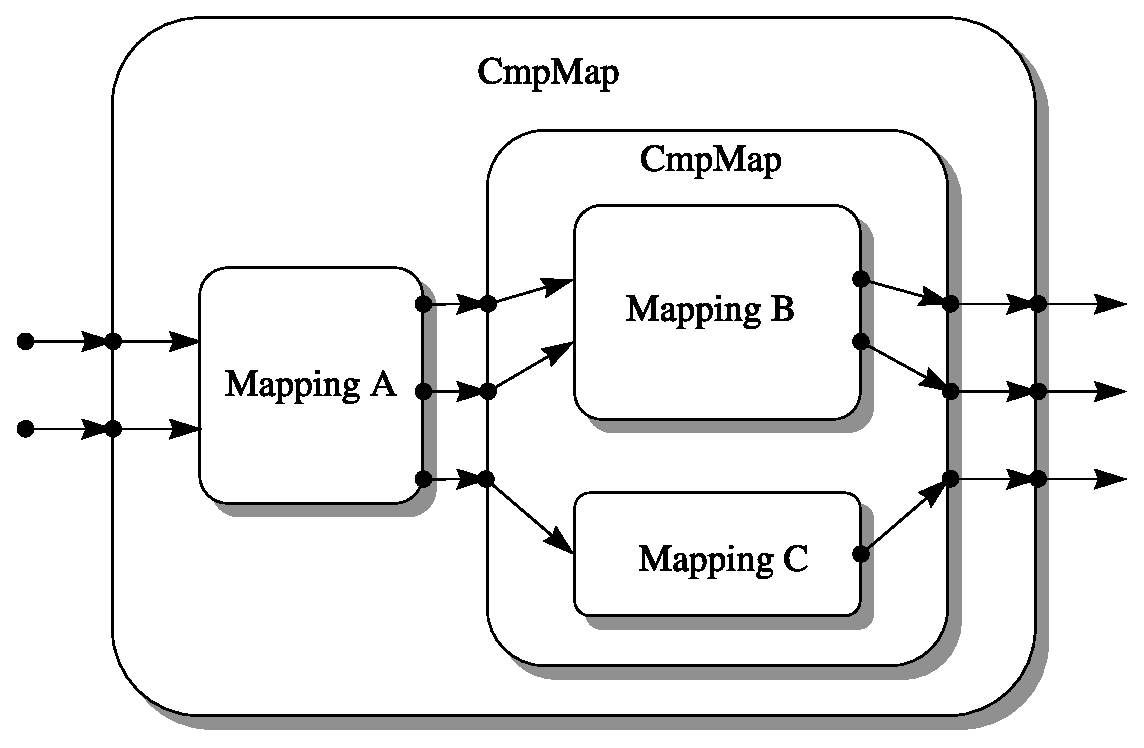
\includegraphics[scale=0.6]{sun210_figures/complex.eps}
   \caption{CmpMaps (compound Mappings) may be nested in order to
   construct complex Mappings out of simpler building blocks.}
   \label{fig:complexcmpmap}
   \end{center}
   \end{figure}
   This gives AST great flexibility in the coordinate transformations it
   can describe.
\end{latexonly}
\begin{htmlonly}
   The CmpMap forms the key to building arbitrarily complex Mappings
   because it is itself a form of Mapping. This means that a CmpMap may
   contain other CmpMaps as components ({\em{e.g.}}\ the Figure
   below). This nesting of CmpMaps can be repeated indefinitely, so that
   complex Mappings may be built in a hierarchical manner out of simper
   ones.  This gives AST great flexibility in the coordinate
   transformations it can describe.
   \begin{quote}
   \begin{figure}
   \label{fig:complexcmpmap}
   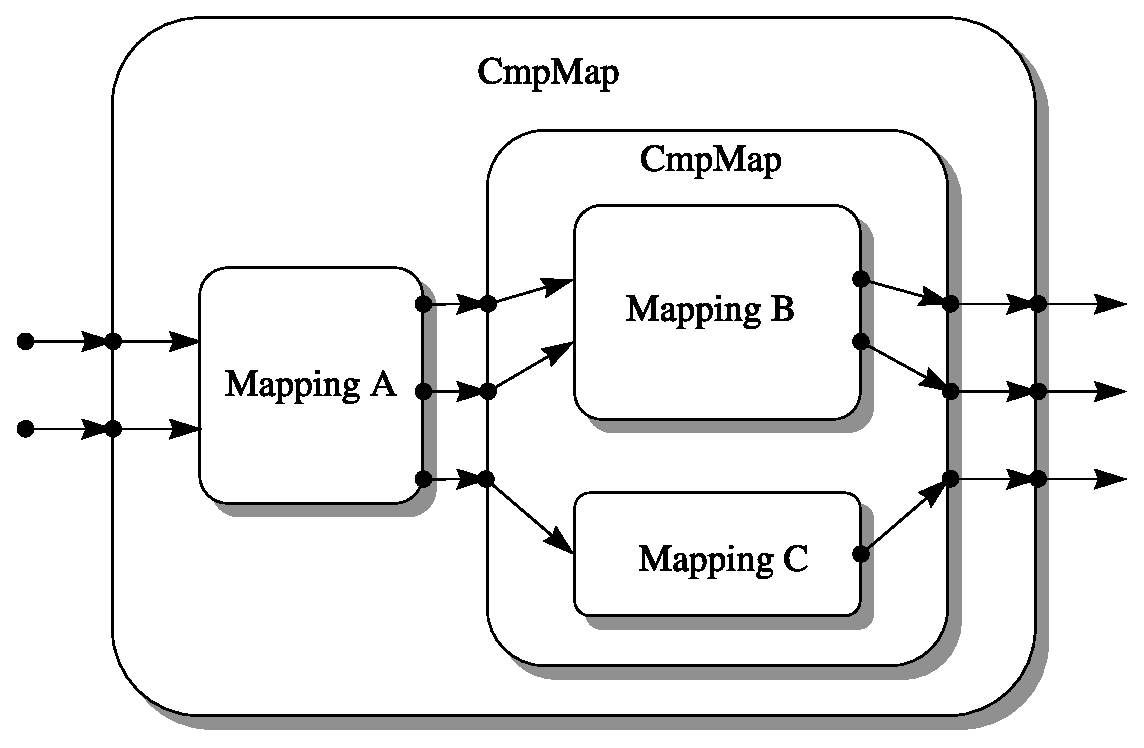
\includegraphics[scale=0.8]{sun210_figures/complex.eps}
   \caption{CmpMaps (compound Mappings) may be nested in order to
   construct complex Mappings out of simpler building blocks.}
   \end{figure}
   \end{quote}
\end{htmlonly}

{\bf{Further reading:}} For a more complete description of CmpMaps,
see \secref{ss:cmpmaps}. Also see the CmpMap entry in
\appref{ss:classdescriptions}.

\subsection{Representing Coordinate Systems}

\begin{latexonly}
   While Mappings (\secref{ss:mappingoverview}) represent the
   relationships between coordinate systems in AST, the coordinate
   systems themselves are represented by Objects called Frames
   (Figure~\ref{fig:frames}).
   \begin{figure}
   \begin{center}
   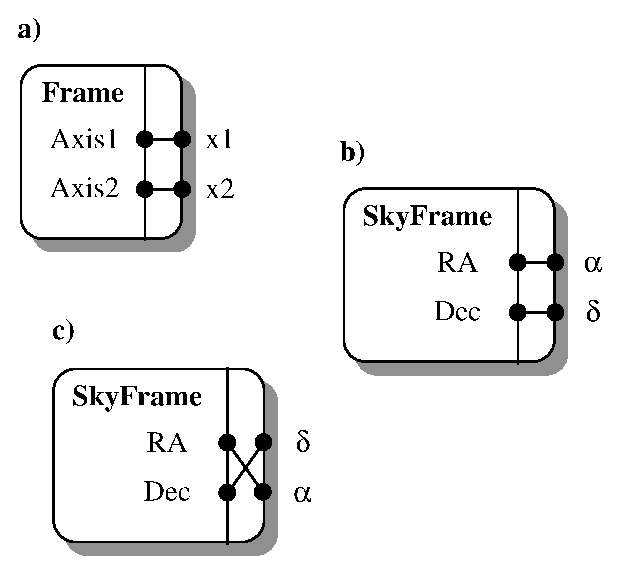
\includegraphics[scale=0.75]{sun210_figures/frames.eps}
   \caption{(a) A basic \htmlref{Frame}{Frame} is used to represent a Cartesian coordinate
   system, here 2-dimensional. (b) A \htmlref{SkyFrame}{SkyFrame} represents a (spherical)
   celestial coordinate system. (c) The axis order of any Frame may be
   permuted to match the coordinate space it describes.}
   \label{fig:frames}
   \end{center}
   \end{figure}
\end{latexonly}
\begin{htmlonly}
   While Mappings (\secref{ss:mappingoverview}) represent the
   relationships between coordinate systems in AST, the coordinate
   systems themselves are represented by Objects called Frames (see
   Figure below).
   \begin{quote}
   \begin{figure}
   \label{fig:frames}
   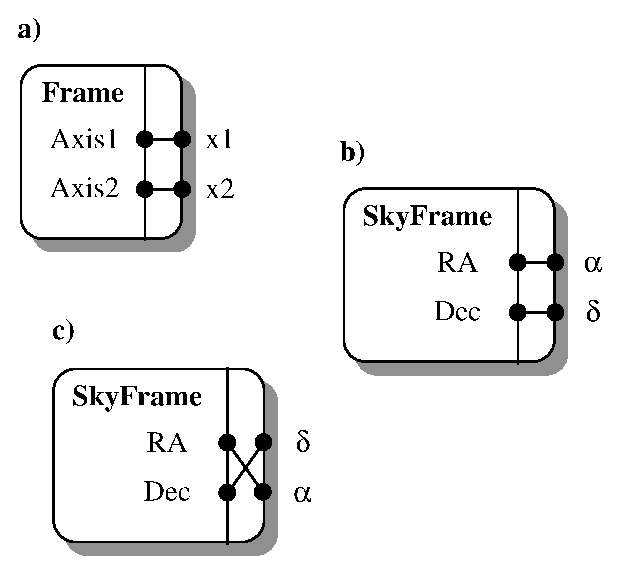
\includegraphics[scale=1.5]{sun210_figures/frames.eps}
   \caption{(a) A basic Frame is used to represent a Cartesian coordinate
   system, here 2-dimensional. (b) A SkyFrame represents a (spherical)
   celestial coordinate system. (c) The axis order of any Frame may be
   permuted to match the coordinate space it describes.}
   \end{figure}
   \end{quote}
\end{htmlonly}
A Frame is similar in concept to the frame you might draw around a
graph.  It contains information about the labels which appear on the
axes, the axis units, a title, knowledge of how to format the
coordinate values on each axis, {\em{etc.}}  An AST Frame is not,
however, restricted to two dimensions and may have any number of axes.

A basic Frame may be used to represent a Cartesian coordinate system
by setting values for its {\em attributes} (all AST Objects have
values associated with them called attributes, which may be set and
enquired).  Usually, this would involve setting appropriate axis
labels and units, for example.  Routines are provided for use with
Frames to perform operations such as formatting coordinate values as
text, calculating distances between points, interchanging axes,
{\em{etc.}}

There are several more specialised forms of Frame, which provide the
additional functionality required when handling coordinates within some
specific physical domain. This ranges from tasks such as formatting axis
values, to complex tasks such as determining the transformation between
any pair of related coordinate systems. For instance, the SkyFrame
(Figure~\ref{fig:frames}b,c), represents celestial coordinate systems,
the \htmlref{SpecFrame}{SpecFrame} represents spectral coordinate systems, and the \htmlref{TimeFrame}{TimeFrame}
represents time coordinate systems. All these provide a wide range of
different systems for describing positions within their associated physical
domain, and these may be selected by setting appropriate attributes.

\begin{latexonly}
   As with compound Mappings (\secref{ss:cmpmapoverview}), it is possible
   to merge two Frames together to form a compound Frame, or \htmlref{CmpFrame}{CmpFrame}, in
   which both sets of axes are combined.  One could, for example, have
   celestial coordinates on two axes and an unrelated coordinate
   (wavelength, perhaps) on a third (Figure~\ref{fig:cmpframe}).
   Knowledge of the relationships between the axes is preserved
   internally by the process of constructing the CmpFrame which
   represents them.
   \begin{figure}
   \begin{center}
   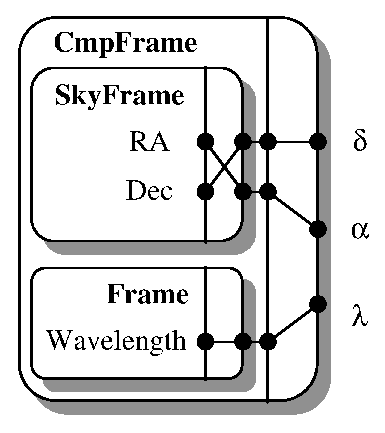
\includegraphics[scale=0.85]{sun210_figures/cmpframe.eps}
   \caption{A CmpFrame (compound Frame) formed by combining two simpler
   Frames. Note how the special relationship which exists between the RA
   and Dec axes is preserved within this data structure. As with compound
   Mappings (Figure~\ref{fig:complexcmpmap}), CmpFrames may be nested in
   order to build more complex Frames.}
   \label{fig:cmpframe}
   \end{center}
   \end{figure}
\end{latexonly}
\begin{htmlonly}
   As with compound Mappings (\secref{ss:cmpmapoverview}), it is possible
   to merge two Frames together to form a compound Frame, or CmpFrame, in
   which both sets of axes are combined.  One could, for example, have
   celestial coordinates on two axes and an unrelated coordinate
   (wavelength, perhaps) on a third (see Figure below).  Knowledge of the
   relationships between the axes is preserved internally by the process
   of constructing the CmpFrame which represents them.
   \begin{quote}
   \begin{figure}
   \label{fig:cmpframe}
   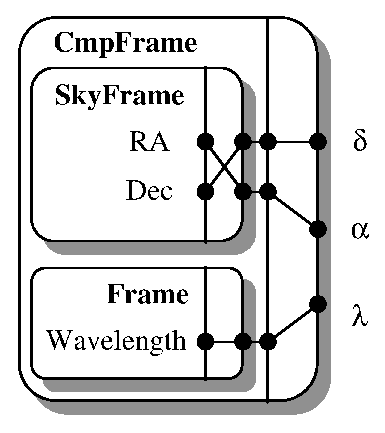
\includegraphics[scale=1.5]{sun210_figures/cmpframe.eps}
   \caption{A CmpFrame (compound Frame) formed by combining two simpler
   Frames. Note how the special relationship which exists between the RA
   and Dec axes is preserved within this data structure. As with compound
   Mappings (Figure~\ref{fig:complexcmpmap}), CmpFrames may be nested in
   order to build more complex Frames.}
   \end{figure}
   \end{quote}
\end{htmlonly}

{\bf{Further reading:}} For a more complete description of Frames see
\secref{ss:frames}, for SkyFrames see \secref{ss:skyframes} and for
SpecFrames see \secref{ss:specframes}.  Also see the Frame, SkyFrame,
SpecFrame, TimeFrame and CmpFrame entries in \appref{ss:classdescriptions}.

\subsection{Networks of Coordinate Systems}

\begin{latexonly}
   Mappings and Frames may be connected together to form networks called
   FrameSets, which are used to represent sets of inter-related
   coordinate systems (Figure~\ref{fig:frameset}).
   \begin{figure}
   \begin{center}
   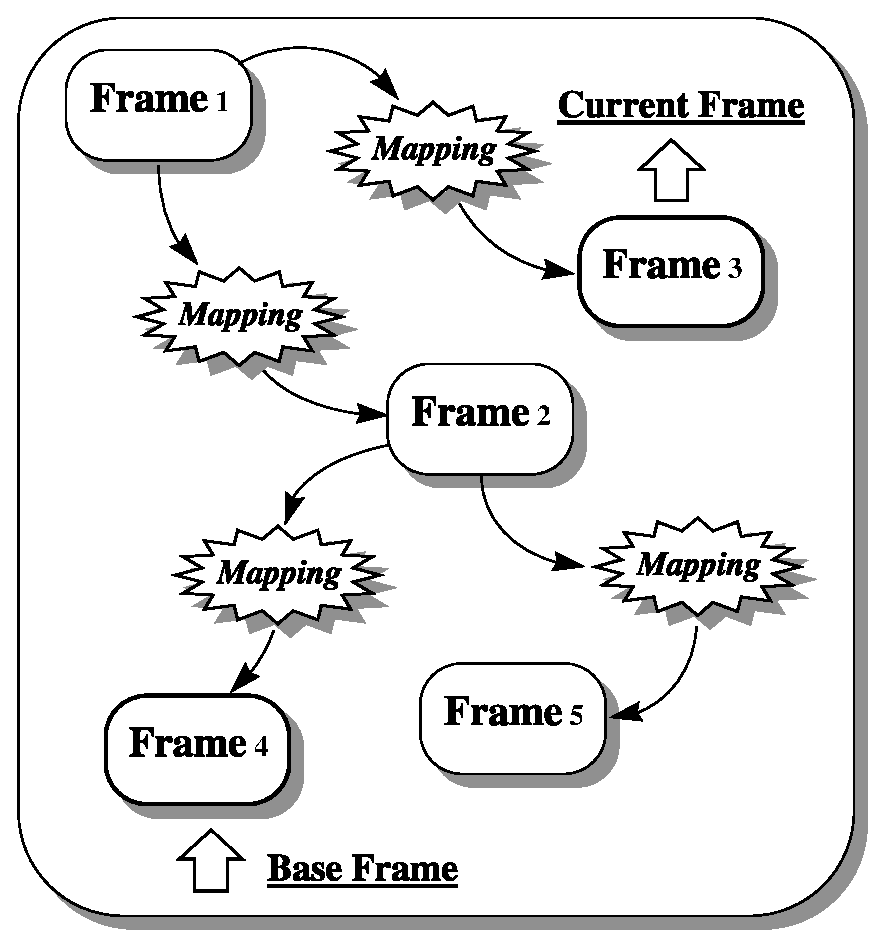
\includegraphics[scale=0.75]{sun210_figures/frameset.eps}
   \caption{A \htmlref{FrameSet}{FrameSet} is a network of Frames inter-connected by Mappings
   such that there is exactly one conversion path, {\em{via}} Mappings,
   between any pair of Frames.}
   \label{fig:frameset}
   \end{center}
   \end{figure}
\end{latexonly}
\begin{htmlonly}
   Mappings and Frames may be connected together to form networks called
   FrameSets, which are used to represent sets of inter-related
   coordinate systems (see Figure below).
   \begin{quote}
   \begin{figure}
   \label{fig:frameset}
   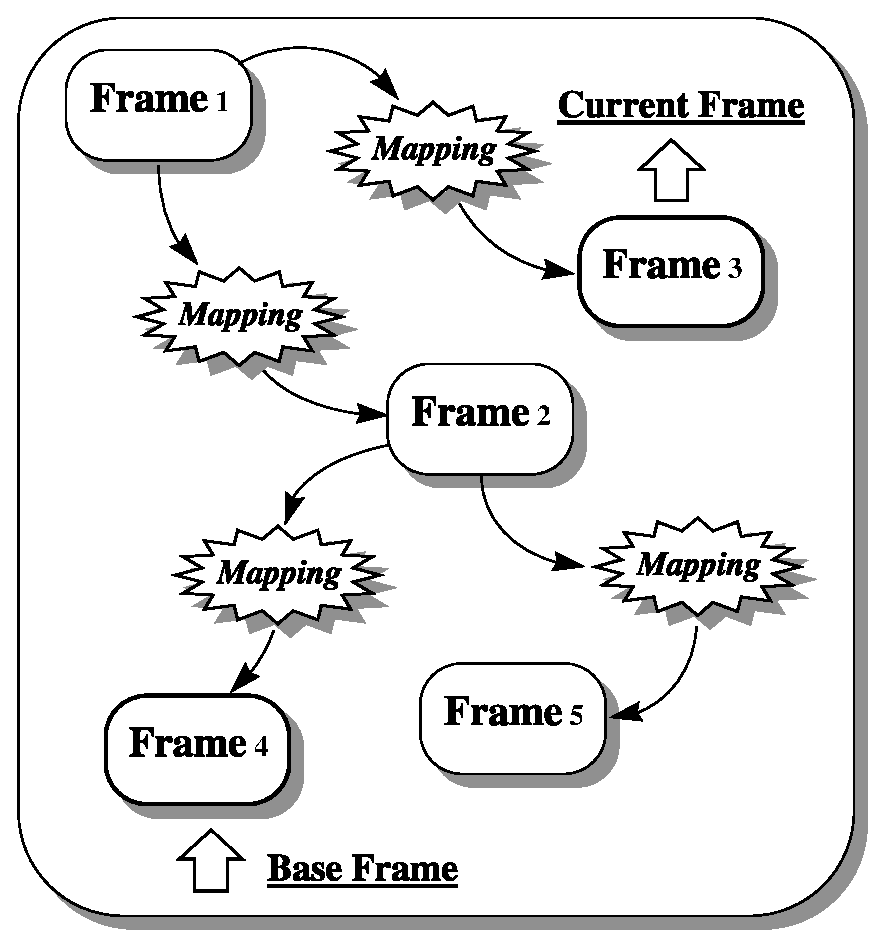
\includegraphics[scale=1.0]{sun210_figures/frameset.eps}
   \caption{A FrameSet is a network of Frames inter-connected by Mappings
   such that there is exactly one conversion path, {\em{via}} Mappings,
   between any pair of Frames.}
   \end{figure}
   \end{quote}
\end{htmlonly}
A FrameSet may be extended by adding a new \htmlref{Frame}{Frame} to it, together with
an associated \htmlref{Mapping}{Mapping} which relates the new coordinate system to one
which is already present.  This process ensures that there is always
exactly one path, {\em{via}} Mappings, between any pair of Frames.  A
function is provided for identifying this path and returning the
complete Mapping.

One of the Frames in a FrameSet is termed its {\em{base}} Frame.  This
underlies the FrameSet's purpose, which is to calibrate datasets and
other entities by attaching coordinate systems to them.  In this
context, the base Frame represents the ``native'' coordinate system
(for example, the pixel coordinates of an image).  Similarly, one
Frame is termed the {\em{current}} Frame and represents the
``currently-selected'' coordinates.  It might, typically, be a
celestial or spectral coordinate system and would be used during
interactions with
a user, as when plotting axes on a graph or producing a table of
results.  Other Frames within the FrameSet represent a library of
alternative coordinate systems which a software user can select by
making them current.

{\bf{Further reading:}} For a more complete description of
FrameSets, see \secref{ss:framesets} and \secref{ss:fshigher}. Also
see the FrameSet entry in \appref{ss:classdescriptions}.

\subsection{Input/Output Facilities}

AST allows you to convert any kind of \htmlref{Object}{Object} into a stream of text
which contains a full description of that Object. This text may be
written out by one program and read back in by another, thus allowing
the original Object to be reconstructed.

The filter which converts Objects into text and back again is itself a
kind of Object, called a \htmlref{Channel}{Channel}. A Channel provides a number of
options for controlling the information content of the text, such as
the addition of comments for human interpretation.  It is also
possible to intercept the text being processed by a Channel so that it
may be redirected to/from any chosen external data store, such as a
text file, an astronomical dataset, or a network connection.

The text format used by the basic Channel class is peculiar to the AST
library - no other software will understand it. However, more specialised
forms of Channel are provided which use text formats more widely
understood.

To further facilitate the storage of coordinate system information in
astronomical datasets, a more specialised form of Channel called a
\htmlref{FitsChan}{FitsChan} is provided. Instead of using free-format text, a FitsChan
converts AST Objects to and from FITS header cards. It also allows the
information to be encoded in the FITS cards in a number of ways
(called {\em{encodings}}), so that WCS information from a variety of
sources can be handled.

Another sub-class of Channel, called \htmlref{XmlChan}{XmlChan}, is a specialised form of
Channel that stores the text in the form of XML markup. Currently, two
markup formats are provided by the XmlChan class, one is closely related
to the text format produced by the basic Channel class (currently, no
schema or DTD is available describing this format). The other is a subset
of an early draft of the IVOA Space-Time-Coordinates XML (STC-X) schema
(V1.20) described at \htmladdnormallink{
http://www.ivoa.net/Documents/WD/STC/STC-20050225.html
}{
http://www.ivoa.net/Documents/WD/STC/STC-20050225.html
}\footnote{XML documents which use only the subset of the STC schema
supported by AST can be read by the XmlChan class to produce
corresponding AST objects (subclasses of the \htmlref{Stc}{Stc} class). However, the
reverse is not possible. That is, AST objects can not currently be
written out in the form of STC documents.}. The version of STC-X that has
been adopted by the IVOA differs in several significant respects from
V1.20, and therefore this XmlChan format is of historical interest only.

Finally, the \htmlref{StcsChan}{StcsChan} class provides facilities for reading and writing
IVOA STC-S region descriptions. STC-S (see \htmladdnormallink{
http://www.ivoa.net/Documents/latest/STC-S.html}{
http://www.ivoa.net/Documents/latest/STC-S.html}) is a linear string
syntax that allows simple specification of STC metadata. AST supports a
subset of the STC-S specification, allowing an STC-S description of a
region within an AST-supported astronomical coordinate system to be converted
into an equivalent AST \htmlref{Region}{Region} object, and vice-versa.

{\bf{Further reading:}} For a more complete description of Channels
see \secref{ss:channels} and for FitsChans see \secref{ss:nativefits}
and \secref{ss:foreignfits}. Also see the Channel and FitsChan entries
in \appref{ss:classdescriptions} and the \htmlref{Encoding}{Encoding} entry in
\appref{ss:attributedescriptions}.

\subsection{Producing Graphical Output}

Graphical output is supported by a specialised form of \htmlref{FrameSet}{FrameSet} called
a \htmlref{Plot}{Plot}, whose base \htmlref{Frame}{Frame} corresponds with the native coordinates of
the underlying graphics system.  Plotting operations are specified in
{\em{physical coordinates}} which correspond with the Plot's current
Frame. Typically, this might be a celestial coordinate system.

Operations, such as drawing lines, are automatically transformed from
physical to graphical coordinates before plotting, using an adaptive
algorithm which ensures smooth curves (because the transformation is
usually non-linear).  ``Missing'' coordinates ({\em{e.g.}}\ graphical
coordinates which do not project on to the celestial sphere),
discontinuities and generalised clipping are all consistently handled.
It is possible, for example, to plot in equatorial coordinates and
clip in galactic coordinates.  The usual plotting operations are
provided (text, markers), but a geodesic curve replaces the primitive
straight line element.  There is also a separate function for drawing
axis lines, since these are normally not geodesics.

In addition to drawing coordinate grids over an area of the sky, another
common use of the Plot class is to produce line plots such as flux
against wavelength, displacement again time, \emph{etc}. For these
situations the current Frame of the Plot would be a compound Frame
(\htmlref{CmpFrame}{CmpFrame}) containing a pair of 1-dimensional Frames - the first
representing the X axis quantity (wavelength, time, etc), and the second
representing the Y axis quantity (flux, displacement, etc). The Plot
class includes an option for axes to be plotted logarithmically.

\begin{latexonly}
   Perhaps the most useful graphics function available is for drawing
   fully annotated coordinate grids ({\em{e.g.}}\ Figure~\ref{fig:gridplot}).
   \begin{figure}
   \begin{center}
   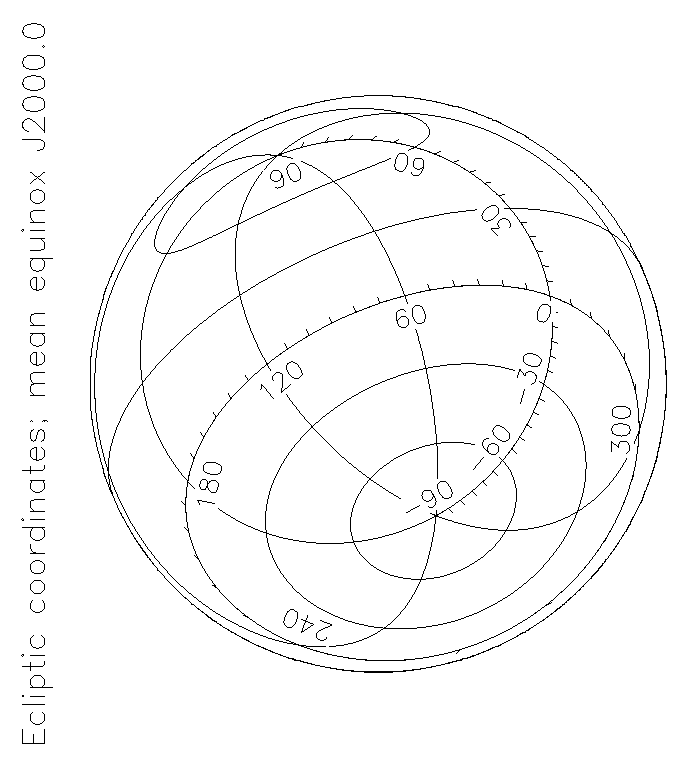
\includegraphics[scale=0.8,angle=-90]{sun210_figures/gridplot_bw.eps}
   \caption{A labelled coordinate grid for an all-sky zenithal equal area
   projection in ecliptic coordinates. This was composed and drawn
   {\em{via}} a Plot using a
   single subroutine call.}
   \label{fig:gridplot}
   \end{center}
   \end{figure}
\end{latexonly}
\begin{htmlonly}
   Perhaps the most useful graphics function available is for drawing
   fully annotated coordinate grids ({\em{e.g.}}\ the Figure below).
   \begin{quote}
   \begin{figure}
   \label{fig:gridplot}
   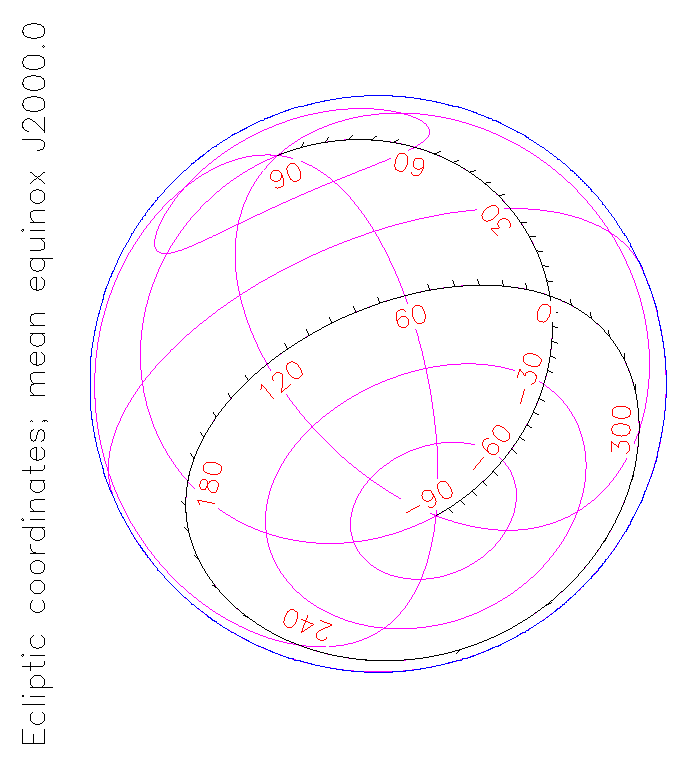
\includegraphics[scale=1.2,angle=-90]{sun210_figures/gridplot.eps}
   \caption{A labelled coordinate grid for an all-sky zenithal equal area
   projection in ecliptic coordinates. This was composed and drawn
   {\em{via}} a Plot using a
   single subroutine call.}
   \end{figure}
   \end{quote}
\end{htmlonly}
This uses a general algorithm which does not depend on knowledge of
the coordinates being represented, so can also handle
programmer-defined coordinate systems.  Grids for all-sky projections,
including polar regions, can be drawn and most aspects of the output
(colour, line style, {\em{etc.}}) can be adjusted by setting
appropriate Plot attributes.

{\bf{Further reading:}} For a more complete description of
Plots and how to produce graphical output, see \secref{ss:plots}. Also
see the Plot entry in \appref{ss:classdescriptions}.

\cleardoublepage
\section{\label{ss:howto}How To\ldots}

For those of you with a plane to catch, this section provides some
instant templates and recipes for performing the most
commonly-required operations using AST, but without going into
detail. The examples given (sort of) follow on from each other, so you
should be able to construct a variety of programs by piecing them
together.  Note that some of them appear longer than they actually
are, because we have included plenty of comments and a few options
that you probably won't need.

If any of this material has you completely baffled, then you may want
to read the introduction to AST programming concepts in
\secref{ss:primer} first. Otherwise, references to more detailed
reading are given after each example, just in case they don't quite do
what you want.

\subsection{\ldots Obtain and Install AST}
The AST library is available both as a stand-alone package and also as
part of the Starlink Software Collection\footnote{The Starlink Software
Collection can be downloaded from
\htmladdnormallink{http://www.starlink.ac.uk/Download/}
{http://www.starlink.ac.uk/Download/}.}. If your site has the Starlink
Software Collection installed then AST should already be available.

If not, you can download the AST library by itself from
\htmladdnormallink{http://www.starlink.ac.uk/ast/}
{http://www.starlink.ac.uk/ast/}.

\subsection{\ldots Structure an AST Program}

An AST program normally has the following structure:

\small
\begin{verbatim}
*  Include the interface to the AST library.
      INCLUDE 'AST_PAR'

*  Declare an integer status variable.
      INTEGER STATUS
      <maybe other declarations>

*  Initialise the status to zero.
      STATUS = 0
      <maybe some Fortran statements>

*  Enclose the parts which use AST between AST_BEGIN and AST_END calls.
      CALL AST_BEGIN( STATUS )
      <Fortran statements which use AST>
      CALL AST_END( STATUS )

      <maybe more Fortran statements>
      END
\end{verbatim}
\normalsize

The use of \htmlref{AST\_BEGIN}{AST_BEGIN} and \htmlref{AST\_END}{AST_END} is optional, but has the effect of
tidying up after you have finished using AST, so is normally
recommended. For more details of this, see \secref{ss:contexts}. For
details of how to access the AST\_PAR include file, see
\secref{ss:accessingheaderfile}.

\subsection{\label{ss:howtobuild}\ldots Build an AST Program}

To build a simple AST program that doesn't use graphics, use:

\begin{quote}
\small
\begin{verbatim}
f77 program.f -L/star/lib -I/star/include `ast_link` -o program
\end{verbatim}
\normalsize
\end{quote}

On Linux systems you should usually use \verb+g77 -fno-second-underscore+ in
place of \verb+f77+ - see \xref{``Software development on Linux''}{sun212}
{software_development_on_linux} in \xref{SUN/212}{sun212}{}.

To build a program which uses PGPLOT for graphics, use:

\begin{quote}
\small
\begin{verbatim}
f77 program.f -L/star/lib `ast_link -pgplot` -o program
\end{verbatim}
\normalsize
\end{quote}

again using \verb+g77 -fno-second-underscore+ in place of \verb+f77+
on Linux systems.

For more details about accessing AST include files, see
\secref{ss:accessingheaderfile}. For more
details about linking programs, see \secref{ss:linking} and the
description of the ``\htmlref{ast\_link}{ast_link}'' command in
\appref{ss:commanddescriptions}.

\subsection{\label{ss:howtoreadwcs}\ldots Read a WCS Calibration from a Dataset}


Precisely how you extract world coordinate system (WCS) information
from a dataset obviously depends on what type of dataset it
is. Usually, however, you should be able to obtain a set of FITS
header cards which contain the WCS information (and probably much more
besides). Suppose that CARDS is an array of character strings
containing a complete set of FITS header cards and NCARD is the number
of cards. Then proceed as follows:

\small
\begin{verbatim}
      INTEGER FITSCHAN, ICARD, NCARD, WCSINFO
      CHARACTER * ( 80 ) CARDS( NCARD )

      ...

*  Create a FitsChan and fill it with FITS header cards.
      FITSCHAN = AST_FITSCHAN( AST_NULL, AST_NULL, ' ', STATUS )
      DO 1 ICARD = 1, NCARD
         CALL AST_PUTFITS( FITSCHAN, CARDS( ICARD ), .FALSE., STATUS )
 1    CONTINUE

*  Rewind the FitsChan and read WCS information from it.
      CALL AST_CLEAR( FITSCHAN, 'Card', STATUS )
      WCSINFO = AST_READ( FITSCHAN, STATUS )
\end{verbatim}
\normalsize

The result should be a pointer, WCSINFO, to a \htmlref{FrameSet}{FrameSet} which contains
the WCS information. This pointer can now be used to perform many
useful tasks, some of which are illustrated in the following recipes.

Some datasets which do not easily yield FITS header cards may require
a different approach, possibly involving use of a \htmlref{Channel}{Channel} or \htmlref{XmlChan}{XmlChan}
(\secref{ss:channels}) rather than a \htmlref{FitsChan}{FitsChan}. In the case of the
Starlink NDF data format, for example, all the above may be replaced
by a single call to the routine
\xref{NDF\_GTWCS}{sun33}{NDF_GTWCS}---see \xref{SUN/33}{sun33}{}.  The
whole process can probably be encapsulated in a similar way for most
other data systems, whether they use FITS header cards or not.

For more details about reading WCS information from datasets, see
\secref{ss:identifyingfitsencoding} and
\secref{ss:readingforeignfits}. For a more general description of
FitsChans and their use with FITS header cards, see
\secref{ss:nativefits} and \secref{ss:foreignfits}. For more details
about FrameSets, see \secref{ss:framesets} and \secref{ss:fshigher}.

\subsection{\ldots Validate WCS Information}

Once you have read WCS information from a dataset, as in
\secref{ss:howtoreadwcs}, you may wish to check that you have been
successful. The following will detect and classify the things that
might possibly go wrong:

\small
\begin{verbatim}
      IF ( STATUS .NE. 0 ) THEN
         <an error occurred (a message will have been issued)>
      ELSE IF ( WCSINFO .EQ. AST__NULL ) THEN
         <there was no WCS information present>
      ELSE IF ( AST_GETC( WCSINFO, 'Class', STATUS ) .NE. 'FrameSet' ) THEN
         <something unexpected was read (i.e. not a FrameSet)>
      ELSE
         <WCS information was read OK>
      END IF
\end{verbatim}
\normalsize

For more information about detecting errors in AST routines, see
\secref{ss:errordetection}. For details of how to validate input data
read by AST, see \secref{ss:validatinginput} and
\secref{ss:readingforeignfits}.

\subsection{\ldots Display AST Data}

If you have a pointer to any AST \htmlref{Object}{Object}, you can display the data
stored in that Object in textual form as follows:

\small
\begin{verbatim}
      CALL AST_SHOW( WCSINFO, STATUS )
\end{verbatim}
\normalsize

Here, we have used a pointer to the \htmlref{FrameSet}{FrameSet} which we read earlier
(\secref{ss:howtoreadwcs}).  The result is written to the program's
standard output stream. This can be very useful during debugging.

For more details about using \htmlref{AST\_SHOW}{AST_SHOW}, see
\secref{ss:displayingobjects}. For information about interpreting the
output, also see \secref{ss:textualoutputformat}.

\subsection{\label{ss:howtotransform}\ldots Convert Between Pixel and World Coordinates}

You may use a pointer to a \htmlref{FrameSet}{FrameSet}, such as we read in
\secref{ss:howtoreadwcs}, to transform a set of points between the
pixel coordinates of an image and the associated world coordinates. If
you are working in two dimensions, proceed as follows:

\small
\begin{verbatim}
      INTEGER N
      DOUBLE PRECISION XPIXEL( N ), YPIXEL( N )
      DOUBLE PRECISION XWORLD( N ), YWORLD( N )

      ...

      CALL AST_TRAN2( WCSINFO, N, XPIXEL, YPIXEL, .TRUE.,
     :                            XWORLD, YWORLD, STATUS )
\end{verbatim}
\normalsize

Here, N is the number of points to be transformed, XPIXEL and YPIXEL
hold the pixel coordinates, and XWORLD and YWORLD receive the returned
world coordinates.\footnote{By pixel coordinates, we mean a coordinate
system in which the first pixel in the image is centred on (1,1) and
each pixel is a unit square.  Note that the world coordinates will not
necessarily be celestial coordinates, but if they are, then they will
be in radians.}  To transform in the opposite direction, interchange
the two pairs of arrays (so that the world coordinates are given as
input) and change the fifth argument of \htmlref{AST\_TRAN2}{AST_TRAN2} to .FALSE..

To transform points in one dimension, use \htmlref{AST\_TRAN1}{AST_TRAN1}. In any other
number of dimensions (or if the number of dimensions is initially
unknown), use \htmlref{AST\_TRANN}{AST_TRANN}. These routines are described in
\appref{ss:functiondescriptions}.

For more information about transforming coordinates, see
\secref{ss:transforming} and \secref{ss:framesetasmapping}. For
details of how to handle missing coordinates, see
\secref{ss:badcoordinates}.

\subsection{\label{ss:howtotestforcelestial}\ldots Test if a WCS is a Celestial Coordinate System}

The world coordinate system (WCS) currently associated with an image
may often be a celestial coordinate system, but this need not
necessarily be the case. For instance, instead of right ascension and
declination, an image might have a WCS with axes representing
wavelength and slit position, or maybe just plain old pixels.

If you have obtained a WCS calibration for an image, as in
\secref{ss:howtoreadwcs}, in the form of a pointer WCSINFO to a
\htmlref{FrameSet}{FrameSet}, then you may determine if the current coordinate system is a
celestial one or not, as follows:

\small
\begin{verbatim}
      INTEGER FRAME
      LOGICAL ISSKY

      ...

*  Obtain a pointer to the current Frame and determine if it is a
*  SkyFrame.
      FRAME = AST_GETFRAME( WCSINFO, AST__CURRENT, STATUS )
      ISSKY = AST_ISASKYFRAME( FRAME, STATUS )
      CALL AST_ANNUL( FRAME, STATUS )
\end{verbatim}
\normalsize

This will set ISSKY to .TRUE.\ if the WCS is a celestial coordinate
system, and to .FALSE.\ otherwise.

\subsection{\label{ss:howtotestforspectral}\ldots Test if a WCS is a Spectral Coordinate System}
Testing for a spectral coordinate system is basically the same as testing
for a celestial coordinate system (see the previous section). The one
difference is that you use the
AST\_ISASPECFRAME routine
in place of the
AST\_ISASKYFRAME routine.

\subsection{\label{ss:howtoformatcoordinates}\ldots Format Coordinates for Display}

Once you have converted pixel coordinates into world coordinates
(\secref{ss:howtotransform}), you may want to format them as text
before displaying them. Typically, this would convert from (say)
radians into something more comprehensible. Using the \htmlref{FrameSet}{FrameSet} pointer
WCSINFO obtained in \secref{ss:howtoreadwcs} and a pair of world
coordinates XW and YW ({\em{e.g.}}\ see \secref{ss:howtotransform}),
you could proceed as follows:

\small
\begin{verbatim}
      CHARACTER * ( 20 ) XTEXT, YTEXT
      DOUBLE PRECISION XW, YW

      ...

      XTEXT = AST_FORMAT( WCSINFO, 1, XW, STATUS )
      YTEXT = AST_FORMAT( WCSINFO, 2, YW, STATUS )

      WRITE ( *, 199 ) XTEXT, YTEXT
 199  FORMAT( 'Position = ', A, ', ', A )
\end{verbatim}
\normalsize

Here, the second argument to \htmlref{AST\_FORMAT}{AST_FORMAT} is the axis number.

With celestial coordinates, this will usually result in sexagesimal
notation, such as ``12:34:56.7''. However, the same method may be
applied to any type of coordinates and appropriate formatting will be
employed.

For more information about formatting coordinate values and how to
control the style of formatting used, see
\secref{ss:formattingaxisvalues} and
\secref{ss:formattingskyaxisvalues}. If necessary, also see
\secref{ss:normalising} for details of how to ``normalise'' a set of
coordinates so that they lie within the standard range ({\em{e.g.}}\ 0
to 24 hours for right ascension and $\pm 90^\circ$ for
declination).

\subsection{\ldots Display Coordinates as they are Transformed}

In addition to formatting coordinates as part of a program's output,
you may also want to examine coordinate values while debugging your
program. To save time, you can ``eavesdrop'' on the coordinate values
being processed every time they are transformed. For example, when
using the \htmlref{FrameSet}{FrameSet} pointer WCSINFO obtained in
\secref{ss:howtoreadwcs} to transform coordinates
(\secref{ss:howtotransform}), you could inspect the coordinate values
as follows:

\small
\begin{verbatim}
      CALL AST_SET( WCSINFO, 'Report=1', STATUS )
      CALL AST_TRAN2( WCSINFO, N, XPIXEL, YPIXEL, .TRUE.,
     :                            XWORLD, YWORLD, STATUS )
\end{verbatim}
\normalsize

By setting the FrameSet's \htmlref{Report}{Report} attribute to 1, coordinate
transformations are automatically displayed on the program's standard
output stream, appropriately formatted, for example:

\begin{quote}
\begin{verbatim}
(42.1087, 20.2717) --> (2:06:03.0, 34:22:39)
(43.0197, 21.1705) --> (2:08:20.6, 35:31:24)
(43.9295, 22.0716) --> (2:10:38.1, 36:40:09)
(44.8382, 22.9753) --> (2:12:55.6, 37:48:55)
(45.7459, 23.8814) --> (2:15:13.1, 38:57:40)
(46.6528, 24.7901) --> (2:17:30.6, 40:06:25)
(47.5589, 25.7013) --> (2:19:48.1, 41:15:11)
(48.4644, 26.6149) --> (2:22:05.6, 42:23:56)
(49.3695, 27.5311) --> (2:24:23.1, 43:32:41)
(50.2742, 28.4499) --> (2:26:40.6, 44:41:27)
\end{verbatim}
\end{quote}

For a complete description of the Report attribute, see its entry in
\appref{ss:attributedescriptions}.  For further details of how to set
and enquire attribute values, see \secref{ss:settingattributes} and
\secref{ss:gettingattributes}.

\subsection{\ldots Read Coordinates Entered by a User}

In addition to writing out coordinate values generated by your program
(\secref{ss:howtoformatcoordinates}), you may also need to accept
coordinates entered by a user, or perhaps read from a file. In this
case, you will probably want to allow ``free-format'' input, so that
the user has some flexibility in the format that can be used. You will
probably also want to detect any typing errors.

Let's assume that you want to read a number of lines of text, each
containing the world coordinates of a single point, and to split each
line into individual numerical coordinate values. Using the \htmlref{FrameSet}{FrameSet}
pointer WCSINFO obtained earlier (\secref{ss:howtoreadwcs}), you could
proceed as follows:

\small
\begin{verbatim}
      CHARACTER TEXT * ( 80 )
      DOUBLE PRECISION COORD( 10 )
      INTEGER IAXIS, N, NAXES, T

      ...

*  Obtain the number of coordinate axes (if not already known).
      NAXES = AST_GETI( WCSINFO, 'Naxes', STATUS )

*  Loop to read each line of input text, in this case from the
*  standard input channel (your programming environment will probably
*  provide a better way of reading text than this). Set the index T to
*  the start of each line read.
 2    CONTINUE
      READ( *, '(A)', END=99 ) TEXT
      T = 1

*  Attempt to read a coordinate for each axis.
      DO 3 IAXIS = 1, NAXES
         N = AST_UNFORMAT( WCSINFO, IAXIS, TEXT( T : ), COORD( IAXIS ),
     :                     STATUS )

*  If nothing was read and this is not the first axis and the end of
*  the text has not been reached, try stepping over a separator and
*  reading again.
         IF ( ( N .EQ. 0 ) .AND. ( IAXIS .GT. 1 ) .AND.
     :        ( T .LT. LEN( STRING ) ) ) THEN
            T = T + 1
            N = AST_UNFORMAT( WCSINFO, IAXIS, TEXT( T : ),
                              COORD( IAXIS ), STATUS )
         END IF

*  Quit if nothing was read, otherwise move on to the next coordinate.
         IF ( N .EQ. 0 ) GO TO 4
         T = T + N
 3    CONTINUE
 4    CONTINUE

*  Test for the possible errors that may occur...

*  Error detected by AST (a message will have been issued).
      IF ( STATUS .NE. 0 ) THEN
         GO TO 99

*  Error in input data at character TEXT( T + N : T + N ).
      ELSE IF ( ( T .LT. LEN( STRING ) ) .OR. ( N .EQ. 0 ) ) THEN
         <handle the error, or report your own message here>
         GO TO 99

      ELSE
         <coordinates were read OK>
      END IF

*  Return to read the next input line.
      GO TO 2
 99   CONTINUE
\end{verbatim}
\normalsize

This algorithm has the advantage of accepting free-format input in
whatever style is appropriate for the world coordinates in use (under
the control of the FrameSet whose pointer you provide). For example,
wavelength values might be read as floating point numbers
({\em{e.g.}}\ ``1.047'' or ``4787''), whereas celestial positions
could be given in sexagesimal format ({\em{e.g.}}\ ``12:34:56'' or
``12~34.5'') and would be converted into radians. Individual
coordinate values may be separated by white space and/or any
non-ambiguous separator character, such as a comma.

For more information on reading coordinate values using the
\htmlref{AST\_UNFORMAT}{AST_UNFORMAT} function, see \secref{ss:unformattingaxisvalues}. For
details of how sexagesimal formats are handled, and the forms of input
that may be used for for celestial coordinates, see
\secref{ss:unformattingskyaxisvalues}.

\subsection{\label{ss:howtocreatenewwcs}\ldots Create a New WCS Calibration}

This section describes how to add a WCS calibration to a data set which you
are creating from scratch, rather than modifying an existing data set.

In most common cases, the simplest way to create a new WCS calibration
from scratch is probably to create a set of strings describing the
required calibration in terms of the keywords used by the FITS WCS
standard, and then convert these strings into an AST \htmlref{FrameSet}{FrameSet} describing
the calibration. This FrameSet can then be used for many other purposes, or
simply stored in the data set.

The full FITS-WCS standard is quite involved, currently running to four
separate papers, but the basic kernel is quite simple, involving the
following keywords (all of which end with an integer axis index,
indicated below by $<i>$):

\begin{description}
\item[CRPIX<i>]\mbox{}\\
hold the pixel coordinates at a reference point
\item[CRVAL<i>]\mbox{}\\
hold the corresponding WCS coordinates at the reference point
\item[CTYPE<i>]\mbox{}\\
name the quantity represented by the WCS axes, together with the
projection algorithm used to convert the scaled and rotated pixel coordinates
to WCS coordinates.
\item[CD<i>\_<j>]\mbox{}\\
a set of keywords which specify the elements of a matrix. This matrix scales
pixel offsets from the reference point into the offsets required as input
by the projection algorithm specified by the CTYPE keywords. This matrix
specifies the scale and rotation of the image. If there is no rotation
the off-diagonal elements of the matrix (\emph{e.g.} CD1\_2 and
CD2\_1) can be omitted.
\end{description}

As an example consider the common case of a simple 2D image of the sky in
which north is parallel to the second pixel axis and east parallel to the
(negative) first pixel axis. The image scale is 1.2 arc-seconds per pixel
on both axes, and the image is presumed to have been obtained with a
tangent plane projection. Furthermore, it is known that pixel coordinates
(100.5,98.4) correspond to an RA of 11:00:10 and a Dec. of  -23:26:02.
A suitable set of FITS-WCS header cards could be:

\begin{quote}
\small
\begin{verbatim}
CTYPE1  = 'RA---TAN'       / Axis 1 represents RA with a tan projection
CTYPE2  = 'DEC--TAN'       / Axis 2 represents Dec with a tan projection
CRPIX1  = 100.5            / Pixel coordinates of reference point
CRPIX2  = 98.4             / Pixel coordinates of reference point
CRVAL1  = 165.04167        / Degrees equivalent of "11:00:10" hours
CRVAL2  = -23.433889       / Decimal equivalent of "-23:26:02" degrees
CD1_1   = -0.0003333333    / Decimal degrees equivalent of -1.2 arc-seconds
CD2_2   = 0.0003333333     / Decimal degrees equivalent of 1.2 arc-seconds
\end{verbatim}
\normalsize
\end{quote}

Notes:
\begin{itemize}
\item a FITS header card begins with the keyword name starting at column 1,
has an equals sign in column 9, and the keyword value in columns 11 to 80.
\item string values must be enclosed in single quotes.
\item celestial longitude and latitude must both be specified in decimal degrees.
\item the CD1\_1 value is negative to indicate that RA increases as the
first pixel axis decreases.
\item the (RA,Dec) coordinates will be taken as ICRS coordinates. For FK5
you should add:

\begin{quote}
\small
\begin{verbatim}
RADESYS = 'FK5'
EQUINOX = 2005.6
\end{verbatim}
\normalsize
\end{quote}

The EQUINOX value defaults to J2000.0 if omitted. FK4 can also be used in
place of FK5, in which case EQUINOX defaults to B1950.0.

\end{itemize}

Once you have created these FITS-WCS header card strings, you should
store them in a \htmlref{FitsChan}{FitsChan} and then read the corresponding FrameSet from the
FitsChan. How to do this is described in \secref{ss:howtoreadwcs}.

Having created the WCS calibration, you may want to store it in a data
file. How to do this is described in \secref{ss:howtowritewcs}).\footnote{If
you are writing the WCS calibration to a FITS file you obviously
have the choice of storing the FITS-WCS cards directly.}

If the required WCS calibration cannot be described as a set of FITS-WCS
headers, then a different approach is necessary. In this case, you should
first create a \htmlref{Frame}{Frame} describing pixel coordinates, and store this Frame
in a new FrameSet. You should then create a new Frame describing the
world coordinate system. This Frame may be a specific subclass of Frame such
as a \htmlref{SkyFrame}{SkyFrame} for celestial coordinates, a \htmlref{SpecFrame}{SpecFrame} for spectral
coordinates, a Timeframe for time coordinates, or a \htmlref{CmpFrame}{CmpFrame} for a combination
of different coordinates.
You also need to create a suitable \htmlref{Mapping}{Mapping} which transforms pixel
coordinates into world coordinates. AST provides many different types of
Mappings, all of which can be combined together in arbitrary fashions to
create more complicated Mappings. The WCS Frame should then be added into
the FrameSet, using the Mapping to connect the WCS Frame with the pixel
Frame.

\subsection{\label{ss:howtomodifywcs}\ldots Modify a WCS Calibration}

The usual reason for wishing to modify the WCS calibration associated
with a dataset is that the data have been geometrically transformed in
some way (here, we will assume a 2-dimensional image dataset). This
causes the image features (stars, galaxies, {\em{etc.}}) to move with
respect to the grid of pixels which they occupy, so that any
coordinate systems previously associated with the image become
invalid.

To correct for this, it is necessary to set up a \htmlref{Mapping}{Mapping} which
expresses the positions of image features in the new data grid in
terms of their positions in the old grid. In both cases, the grid
coordinates we use will have the first pixel centred at (1,1) with
each pixel being a unit square.

AST allows you to correct for any type of geometrical transformation
in this way, so long as a suitable Mapping to describe it can be
constructed. For purposes of illustration, we will assume here that
the new image coordinates XNEW and YNEW can be expressed in terms of
the old coordinates XOLD and YOLD as follows:

\small
\begin{verbatim}
      DOUBLE PRECISION XNEW, XOLD, YNEW, YOLD
      DOUBLE PRECISION M( 4 ), Z( 2 )

      ...

      XNEW = XOLD * M( 1 ) + YOLD * M( 2 ) + Z( 1 )
      YNEW = XOLD * M( 3 ) + YOLD * M( 4 ) + Z( 2 )
\end{verbatim}
\normalsize

where M is a 2$\times$2 transformation matrix and Z represents a shift
of origin. This is therefore a general linear coordinate
transformation which can represent displacement, rotation,
magnification and shear.

In AST, it can be represented by concatenating two Mappings. The first
is a \htmlref{MatrixMap}{MatrixMap}, which implements the matrix multiplication. The second
is a \htmlref{WinMap}{WinMap}, which linearly transforms one coordinate window on to
another, but will be used here simply to implement the shift of
origin (alternatively, a \htmlref{ShiftMap}{ShiftMap} could have been used in place of a
WinMap). These Mappings may be constructed and concatenated as follows:

\small
\begin{verbatim}
      DOUBLE PRECISION INA( 2 ), INB( 2 ), OUTA( 2 ), OUTB( 2 )
      INTEGER MATRIXMAP, WINMAP

      ...

*  Set up the corners of a unit square.
      DATA INA / 2 * 0.0D0 /
      DATA INB / 2 * 1.0D0 /

*  The MatrixMap may be constructed directly from the matrix M.
      MATRIXMAP = AST_MATRIXMAP( 2, 2, 0, M, ' ', STATUS )

*  For the WinMap, we take the coordinates of the corners of a unit
*  square (window) and then shift them by the required amounts.
      OUTA( 1 ) = INA( 1 ) + Z( 1 )
      OUTA( 2 ) = INA( 2 ) + Z( 2 )
      OUTB( 1 ) = INB( 1 ) + Z( 1 )
      OUTB( 2 ) = INB( 2 ) + Z( 2 )

*  The WinMap will then implement this shift.
      WINMAP = AST_WINMAP( 2, INA, INB, OUTA, OUTB, ' ', STATUS )

*  Join the two Mappings together, so that they are applied one after
*  the other.
      NEWMAP = AST_CMPMAP( MATRIXMAP, WINMAP, 1, ' ', STATUS )
\end{verbatim}
\normalsize

You might, of course, create any other form of Mapping depending on
the type of geometrical transformation involved. For an overview of
the Mappings provided by AST, see \secref{ss:mappingselection}, and
for a description of the capabilities of each class of Mapping, see
its entry in \appref{ss:classdescriptions}. For an overview of how
individual Mappings may be combined, see \secref{ss:cmpmapoverview}
(\secref{ss:cmpmaps} gives more details).

Assuming you have obtained a WCS calibration for your original image
in the form of a pointer to a \htmlref{FrameSet}{FrameSet}, WCSINFO1
(\secref{ss:howtoreadwcs}), the Mapping created above may be used to
produce a calibration for the new image as follows:

\small
\begin{verbatim}
      INTEGER WCSINFO1, WCSINFO2

      ...

*  If necessary, make a copy of the WCS calibration, since we are
*  about to alter it.
      WCSINFO2 = AST_COPY( WCSINFO1, STATUS )

*  Re-map the base Frame so that it refers to the new data grid
*  instead of the old one.
      CALL AST_REMAPFRAME( WCSINFO2, AST__BASE, NEWMAP, STATUS )
\end{verbatim}
\normalsize

This will produce a pointer, WCSINFO2, to a new FrameSet in which all
the coordinate systems associated with the original image are modified
so that they are correctly registered with your new image instead.

For more information about re-mapping the Frames within a FrameSet,
see \secref{ss:remapframe}. Also see \secref{ss:wcsprocessingexample}
for a similar example to the above, applicable to the case of reducing
the size of an image by binning.

\subsection{\label{ss:howtowritewcs}\ldots Write a Modified WCS Calibration to a Dataset}

If you have modified the WCS calibration associated with a dataset,
such as in the example above (\secref{ss:howtomodifywcs}), then you
will need to write the modified version out along with any new data.

In the same way as when reading a WCS calibration
(\secref{ss:howtoreadwcs}), how you do this will depend on your data
system, but we will assume that you wish to generate a set of FITS
header cards that can be stored with the data. You should usually make
preparations for doing this when you first read the WCS calibration
from your input dataset by modifying the example given in
\secref{ss:howtoreadwcs} as follows:

\small
\begin{verbatim}
      INTEGER FITSCHAN1, WCSINFO1
      CHARACTER * ( 20 ) ENCODE

      ...

*  Create an input FitsChan and fill it with FITS header cards. Note,
*  if you have all the header cards in a single string, use AST_PUTCARDS in
*  place of AST_PUTFITS.
      FITSCHAN1 = AST_FITSCHAN( AST_NULL, AST_NULL, ' ', STATUS )
      DO 1 ICARD = 1, NCARD
         CALL AST_PUTFITS( FITSCHAN1, CARDS( ICARD ), .FALSE., STATUS )
 1    CONTINUE

*  Note which encoding has been used for the WCS information.
      ENCODE = AST_GETC( FITSCHAN1, 'Encoding', STATUS );

*  Rewind the input FitsChan and read the WCS information from it.
      CALL AST_CLEAR( FITSCHAN1, 'Card', STATUS )
      WCSINFO1 = AST_READ( FITSCHAN1, STATUS )
\end{verbatim}
\normalsize

Note how we have added an enquiry to determine how the WCS information
is encoded in the input FITS cards, storing the resulting string in
the ENCODE variable. This must be done {\bf{before}} actually reading
the WCS calibration.


Once you have produced a modified WCS calibration for the output
dataset ({\em{e.g.}}\ \secref{ss:howtomodifywcs}), in the form of a
\htmlref{FrameSet}{FrameSet} identified by the pointer WCSINFO2, you can produce a new
\htmlref{FitsChan}{FitsChan} containing the output FITS header cards as follows:

\small
\begin{verbatim}
      INTEGER FITSCHAN2, JUNK, WCSINFO2

      ...

*  Make a copy of the input FitsChan, AFTER the WCS information has
*  been read from it. This will propagate all the input FITS header
*  cards, apart from those describing the WCS calibration.
      FITSCHAN2 = AST_COPY( FITSCHAN1, STATUS )

*  If necessary, make modifications to the cards in FITSCHAN2
*  (e.g. you might need to change NAXIS1, NAXIS2, etc., to account for
*  a change in image size). You probably only need to do this if your
*  data system does not provide these facilities itself.
      <details not shown - see below>

*  Alternatively, if your data system handles the propagation of FITS
*  header cards to the output dataset for you, then simply create an
*  empty FitsChan to contain the output WCS information alone.
*     FITSCHAN2 = AST_FITSCHAN( AST_NULL, AST_NULL, ' ', STATUS )

*  Rewind the new FitsChan (if necessary) and attempt to write the
*  output WCS information to it using the same encoding method as the
*  input dataset.
      CALL AST_SET( FITSCHAN2, 'Card=1, Encoding=' // ENCODE, STATUS )
      IF ( AST_WRITE( FITSCHAN2, WCSINFO2, STATUS ) .EQ. 0 ) THEN

*  If this didn't work (the WCS FrameSet has become too complex), then
*  use the native AST encoding instead.
         CALL AST_SETC( FITSCHAN2, 'Encoding', 'NATIVE', STATUS );
         JUNK = AST_WRITE( FITSCHAN2, WCSINFO2, STATUS );
      END IF
\end{verbatim}
\normalsize

For details of how to modify the contents of the output FitsChan in
other ways, such as by adding, over-writing or deleting header cards,
see \secref{ss:addressingfitscards}, \secref{ss:addingmulticards}, \secref{ss:addingfitscards} and
\secref{ss:findingandchangingfits}.

Once you have assembled the output FITS cards, you may retrieve them
from the FitsChan that contains them as follows:

\small
\begin{verbatim}
      CHARACTER * ( 80 ) CARD

      ...

      CALL AST_CLEAR( FITSCHAN2, 'Card', STATUS )
 5    CONTINUE
      IF ( AST_FINDFITS( FITSCHAN2, '%f', CARD, .TRUE., STATUS ) ) THEN
         WRITE ( *, '(A)' ) CARD
         GO TO 5
      END IF
\end{verbatim}
\normalsize

Here, we have simply written each card to the standard output unit,
but you would obviously replace this with a subroutine call to store
the cards in your output dataset.

For data systems that do not use FITS header cards, a different
approach may be needed, possibly involving use of a \htmlref{Channel}{Channel} or \htmlref{XmlChan}{XmlChan}
(\secref{ss:channels}) rather than a FitsChan.  In the case of the
Starlink NDF data format, for example, all of the above may be
replaced by a single call to the routine
\xref{NDF\_PTWCS}{sun33}{NDF_PTWCS}---see \xref{SUN/33}{sun33}{}. The
whole process can probably be encapsulated in a similar way for most
other data systems, whether they use FITS header cards or not.

For an overview of how to propagate WCS information through data
processing steps, see \secref{ss:propagatingwcsinformation}.  For more
information about writing WCS information to FitsChans, see
\secref{ss:writingnativefits} and \secref{ss:writingforeignfits}.  For
information about the options for encoding WCS information in FITS
header cards, see \secref{ss:nativeencoding},
\secref{ss:foreignencodings}, and the description of the \htmlref{Encoding}{Encoding}
attribute in \appref{ss:attributedescriptions}.  For a complete
understanding of FitsChans and their use with FITS header cards, you
should read \secref{ss:nativefits} and \secref{ss:foreignfits}.

\subsection{\label{ss:howtoplotgrid}\ldots Display a Graphical Coordinate Grid}

\begin{latexonly}
   A common requirement when displaying image data is to plot an
   associated coordinate grid ({\em{e.g.}}\ Figure~\ref{fig:overgrid})
   over the displayed image.
   \begin{figure}
   \begin{center}
   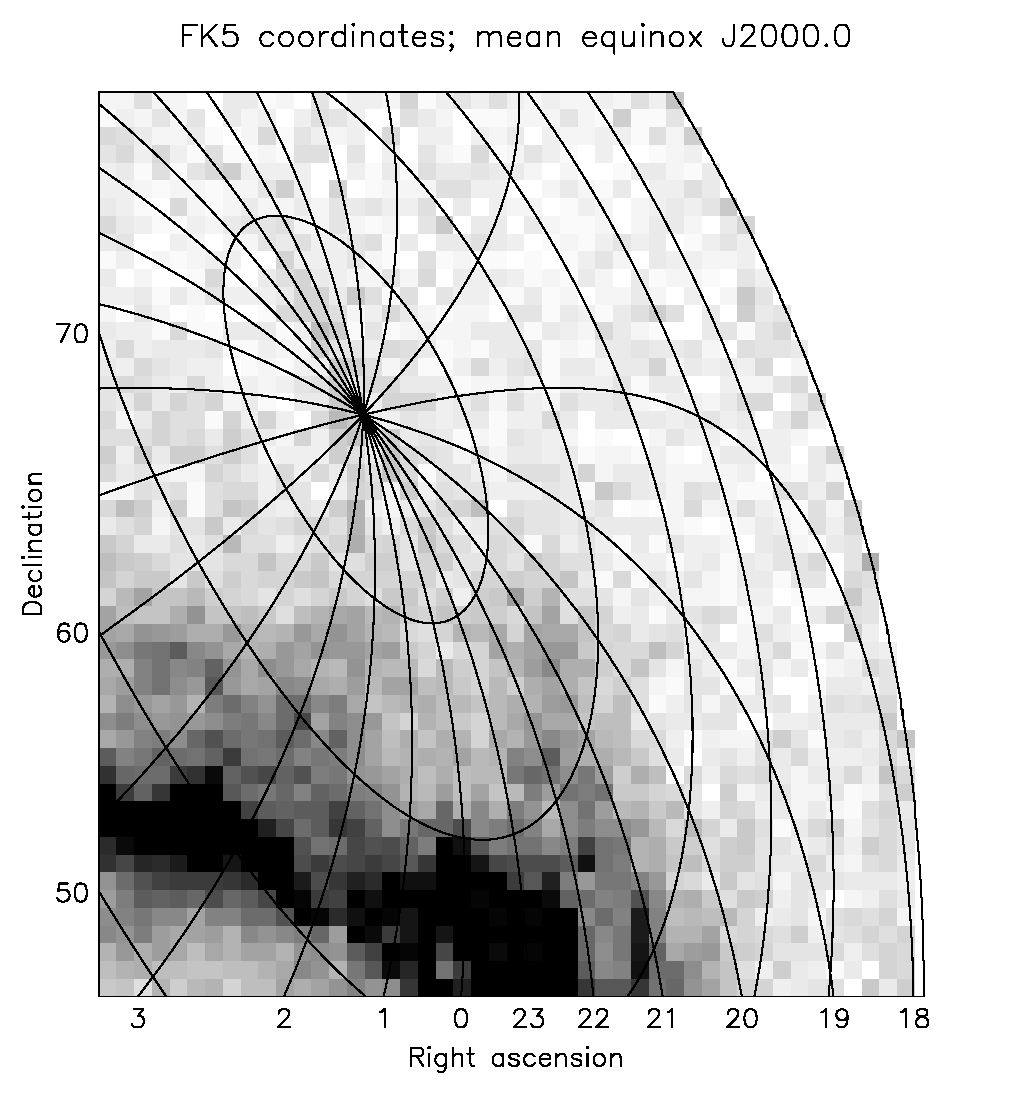
\includegraphics[scale=0.7]{sun210_figures/overgrid_bw.eps}
   \caption{An example of a displayed image with a coordinate grid
   plotted over it.}
   \label{fig:overgrid}
   \end{center}
   \end{figure}
\end{latexonly}
\begin{htmlonly}
   A common requirement when displaying image data is to plot an
   associated coordinate grid over the displayed image ({\em{e.g.}}\
   the following Figure):
   \begin{quote}
   \begin{figure}[bhtp]
   \label{fig:overgrid}
   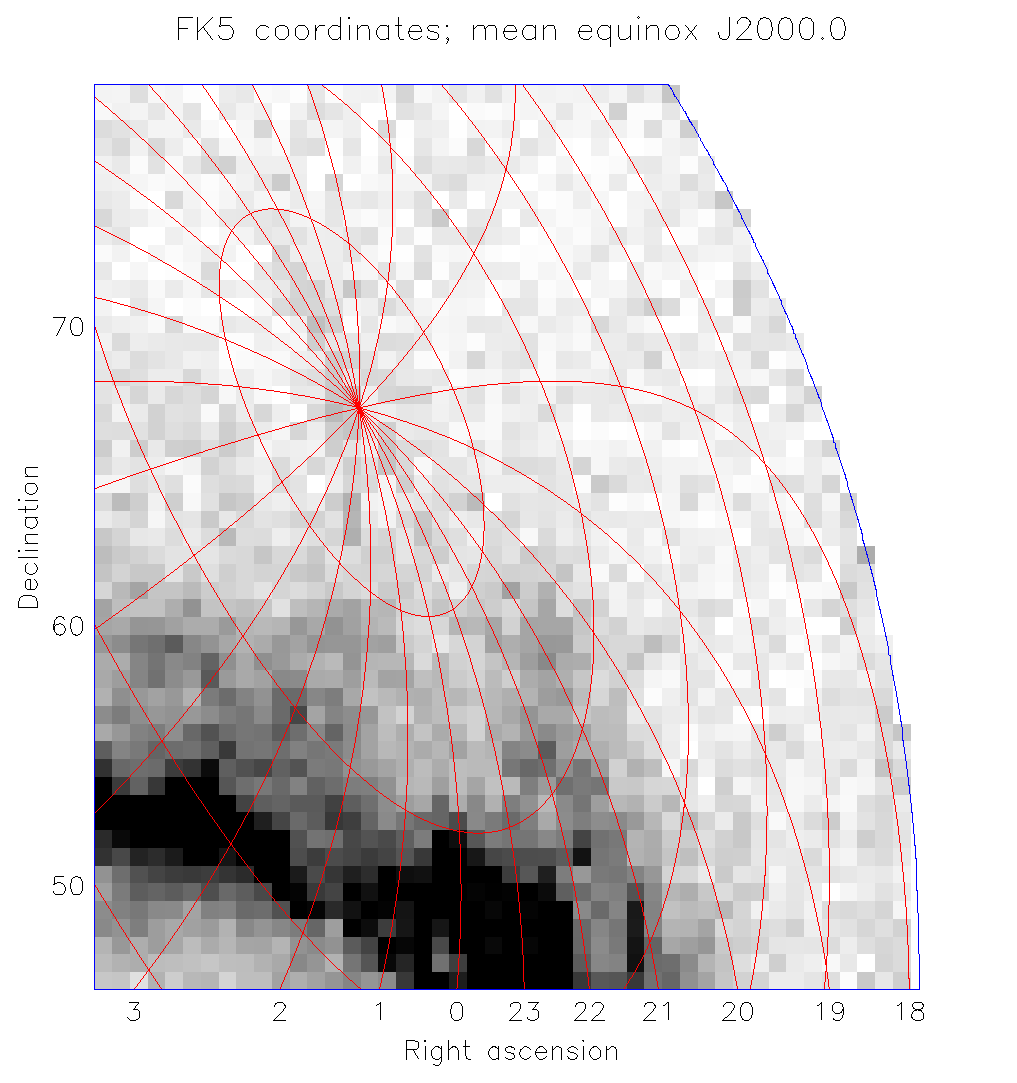
\includegraphics[scale=0.8]{sun210_figures/overgrid.eps}
   \caption{An example of a displayed image with a coordinate grid
   plotted over it.}
   \end{figure}
   \end{quote}
\end{htmlonly}
The use of AST in such circumstances is independent of the underlying
graphics system, so starting up the graphics system, setting up a
coordinate system, displaying the image, and closing down afterwards
can all be done using the graphics routines you would normally use.

However, displaying an image at a precise location can be a little
fiddly with some graphics systems, and obviously the grid drawn by AST
will not be accurately registered with the image unless this is done
correctly. In the following template, we therefore illustrate both
steps, basing the image display on the PGPLOT graphics
package.\footnote{An interface is provided with AST that allows it to
use PGPLOT (\xref{SUN/15}{sun15}{}) for its graphics, although
interfaces to other graphics systems may also be written.}  Plotting a
coordinate grid with AST then becomes a relatively minor part of what
is almost a complete graphics program.

Once again, we assume that a pointer, WCSINFO, to a suitable \htmlref{FrameSet}{FrameSet}
associated with the image has already been obtained
(\secref{ss:howtoreadwcs}).

\small
\begin{verbatim}
      DOUBLE PRECISION BBOX( 4 )
      INTEGER NX, NY, PGBEG, PLOT
      REAL DATA( NX, NY ), GBOX( 4 ), HI, LO, SCALE, TR( 6 )
      REAL X1, X2, XLEFT, XRIGHT, Y1, Y2, YBOTTOM, YTOP

      ...

*  Access the image data, which we assume will be stored in the real
*  2-dimensional array DATA with dimension sizes NX and NY. Also
*  derive limits for scaling it, which we assign to the variables HI
*  and LO.
      <this stage depends on your data system, so is not shown>

*  Open PGPLOT using the device given by environment variable
*  PGPLOT_DEV and check for success.
      IF ( PGBEG( 0, ' ', 1, 1 ) .EQ. 1 ) THEN

*  Clear the screen and ensure equal scales on both axes.
         CALL PGPAGE
         CALL PGWNAD( 0.0, 1.0, 0.0, 1.0 )

*  Obtain the extent of the plotting area (not strictly necessary for
*  PGPLOT, but possibly for other graphics systems). From this, derive
*  the display scale in graphics units per pixel so that the image
*  will fit within the display area.
         CALL PGQWIN( X1, X2, Y1, Y2 )
         SCALE = MIN( ( X2 - X1 ) / NX, ( Y2 - Y1 ) / NY )

*  Calculate the extent of the area in graphics units that the image
*  will occupy, so as to centre it within the display area.
         XLEFT   = 0.5 * ( X1 + X2 - NX * SCALE )
         XRIGHT  = 0.5 * ( X1 + X2 + NX * SCALE )
         YBOTTOM = 0.5 * ( Y1 + Y2 - NY * SCALE )
         YTOP    = 0.5 * ( Y1 + Y2 + NY * SCALE )

*  Set up a PGPLOT coordinate transformation matrix and display the
*  image data as a grey scale map (these details are specific to
*  PGPLOT).
         TR( 1 ) = XLEFT - 0.5 * SCALE
         TR( 2 ) = SCALE
         TR( 3 ) = 0.0
         TR( 4 ) = YBOTTOM - 0.5 * SCALE
         TR( 5 ) = 0.0
         TR( 6 ) = SCALE
         CALL PGGRAY( DATA, NX, NY, 1, NX, 1, NY, HI, LO, TR )

*  BEGINNING OF AST BIT
*  ====================
*  Store the locations of the bottom left and top right corners of the
*  region used to display the image, in graphics coordinates.
         GBOX( 1 ) = XLEFT
         GBOX( 2 ) = YBOTTOM
         GBOX( 3 ) = XRIGHT
         GBOX( 4 ) = YTOP

*  Similarly, store the locations of the image's bottom left and top
*  right corners, in pixel coordinates -- with the first pixel centred
*  at (1,1).
         BBOX( 1 ) = 0.5D0
         BBOX( 2 ) = 0.5D0
         BBOX( 3 ) = NX + 0.5D0
         BBOX( 4 ) = NY + 0.5D0

*  Create a Plot, based on the FrameSet associated with the
*  image. This attaches the Plot to the graphics surface so that it
*  matches the displayed image. Specify that a complete set of grid
*  lines should be drawn (rather than just coordinate axes).
         PLOT = AST_PLOT( WCSINFO, GBOX, BBOX, 'Grid=1', STATUS )

*  Optionally, we can now set other Plot attributes to control the
*  appearance of the grid. The values assigned here use the
*  colour/font indices defined by the underlying graphics system.
         CALL AST_SET( PLOT, 'Colour(grid)=2, Font(textlab)=3', STATUS )

*  Use the Plot to draw the coordinate grid.
         CALL AST_GRID( PLOT, STATUS )

         <maybe some more AST graphics here>

*  Annul the Plot when finished (or use the AST_BEGIN/AST_END
*  technique shown earlier).
         CALL AST_ANNUL( PLOT, STATUS )

*  END OF AST BIT
*  ==============

*  Close down the graphics system.
         CALL PGEND
      END IF
\end{verbatim}
\normalsize

Note that once you have set up a \htmlref{Plot}{Plot} which is aligned with a
displayed image, you may also use it to generate further graphical
output of your own, specified in the image's world coordinate system
(such as markers to represent astronomical objects, annotation,
{\em{etc.}}). There is also a range of Plot attributes which gives
control over most aspects of the output's appearance.  For details of
the facilities available, see \secref{ss:plots} and the description of
the Plot class in \appref{ss:classdescriptions}.

For details of how to build a graphics program which uses PGPLOT, see
\secref{ss:howtobuild} and the description of the \htmlref{ast\_link}{ast_link} command in
\appref{ss:commanddescriptions}.

\subsection{\label{ss:howtoswitchgrid}\ldots Switch to Plot a Different Celestial Coordinate Grid}

Once you have set up a \htmlref{Plot}{Plot} to draw a coordinate grid
(\secref{ss:howtoplotgrid}), it is a simple matter to change things so
that the grid represents a different celestial coordinate system. For
example, after creating the Plot with \htmlref{AST\_PLOT}{AST_PLOT}, you could use:

\small
\begin{verbatim}
      CALL AST_SET( PLOT, 'System=Galactic', STATUS )
\end{verbatim}
\normalsize
or:
\small
\begin{verbatim}
      CALL AST_SET( PLOT, 'System=FK5, Equinox=J2010', STATUS )
\end{verbatim}
\normalsize

and any axes and/or grid drawn subsequently would represent the new
celestial coordinate system you specified.  Note, however, that this
will only work if the original grid represented celestial coordinates
of some kind (see \secref{ss:howtotestforcelestial} for how to
determine if this is the case\footnote{Note that the methods applied
to a \htmlref{FrameSet}{FrameSet} may be used equally well with a Plot.}). If it did not,
you will get an error message.

For more information about the celestial coordinate systems available,
see the descriptions of the \htmlref{System}{System}, \htmlref{Equinox}{Equinox} and \htmlref{Epoch}{Epoch} attributes in
\appref{ss:attributedescriptions}.

\subsection{\ldots Give a User Control Over the Appearance of a Plot}

The idea of using a \htmlref{Plot}{Plot}'s attributes to control the appearance of the
graphical output it produces (\secref{ss:howtoplotgrid} and
\secref{ss:howtoswitchgrid}) can easily be extended to allow the user
of a program complete control over such matters.

For instance, if the file ``plot.config'' contains a series of
plotting options in the form of Plot attribute assignments (see below
for an example), then we could create a Plot and implement these
assignments before producing the graphical output as follows:

\small
\begin{verbatim}
      CHARACTER LINE( 120 )
      INTEGER BASE

      ...

*  Create a Plot and define the default appearance of the graphical
*  output it will produce.
      PLOT = AST_PLOT( WCSINFO, GBOX, PBOX,
     :                 'Grid=1, Colour(grid)=2, Font(textlab)=3',
     :                 STATUS )

*  Obtain the value of any Plot attributes we want to preserve.
      BASE = AST_GETI( PLOT, 'Base', STATUS )

*  Open the plot configuration file, if it exists.
      OPEN ( 1, FILE = 'plot.config', STATUS = 'OLD', ERR = 8 )

*  Read each line of text and use it to set new Plot attribute
*  values. Close the file when done.
 6    CONTINUE
         READ ( 1, '(A)', END = 7 ) LINE
         CALL AST_SET( PLOT, LINE, STATUS )
      GO TO 6
 7    CLOSE ( 1 )
 8    CONTINUE

*  Restore any attribute values we are preserving.
      CALL AST_SETI( PLOT, 'Base', BASE, STATUS )

*  Produce the graphical output (e.g.).
      CALL AST_GRID( PLOT, STATUS )
\end{verbatim}
\normalsize

Notice that we take care that the Plot's \htmlref{Base}{Base} attribute is preserved
so that the user cannot change it. This is because graphical output
will not be produced successfully if the base \htmlref{Frame}{Frame} does not describe
the plotting surface to which we attached the Plot when we created it.

The arrangement shown above allows the contents of the ``plot.config''
file to control most aspects of the graphical output produced
(including the coordinate system used; the colour, line style,
thickness and font used for each component; the positioning of axes
and tick marks; the precision, format and positioning of labels;
{\em{etc.}}) {\em{via}} assignments of the form:

\begin{quote}
\small
\begin{verbatim}
System=Galactic, Equinox = 2001
Border = 1, Colour( border ) = 1
Colour( grid ) = 2
DrawAxes = 1
Colour( axes ) = 3
Digits = 8
Labelling = Interior
\end{verbatim}
\normalsize
\end{quote}

For a more sophisticated interface, you could obviously perform
pre-processing on this input---for example, to translate words like
``red'', ``green'' and ``blue'' into colour indices, to permit
comments and blank lines, {\em{etc.}}

For a full list of the attributes that may be used to control the
appearance of graphical output, see the description of the Plot class
in \appref{ss:classdescriptions}. For a complete description of each
individual attribute ({\em{e.g.}}\ those above), see the attribute's
entry in \appref{ss:attributedescriptions}.

\cleardoublepage
\section{\label{ss:primer}An AST Object Primer}

The AST library deals throughout with entities called Objects and a
basic understanding of how to handle these is needed before you can
use the library effectively.  If you are already familiar with an
object-oriented language, such as C$++$, few of the concepts should
seem new to you.  Be aware, however, that AST is designed to be used
{\em{via}} fairly conventional Fortran and C interfaces, so some
things have to be done a little differently.

If you are not already familiar with object-oriented programming, then
don't worry---we will not emphasise this aspect more than is necessary
and will not assume any background knowledge.  Instead, this section
concentrates on presenting all the fundamental information you will
need, explaining how AST Objects behave and how to manipulate them
from conventional Fortran programs.

If you like to read documents from cover to cover, then you can
consider this section as an introduction to the programming techniques
used in the rest of the document. Otherwise, you may prefer to skim
through it on a first reading and return to it later as reference
material.

\subsection{AST Objects}

An AST \htmlref{Object}{Object} is an entity which is used to store information and
Objects come in various kinds, called {\em{classes,}} according to the
sort of information they hold. Throughout this section, we will make
use of a simple Object belonging to the ``\htmlref{ZoomMap}{ZoomMap}'' class to
illustrate many of the basic concepts.

A ZoomMap is an Object that contains a recipe for converting
coordinates between two hypothetical coordinate systems.  It does this
by multiplying all the coordinate values by a constant called the
{\em{\htmlref{Zoom}{Zoom} factor.}}  A ZoomMap is a very simple Object which exists
mainly for use in examples. It allows us to illustrate the ways in
which Objects are manipulated and to introduce the concept of a
\htmlref{Mapping}{Mapping}---a recipe for converting coordinates---which is fundamental
to the way the AST library works.

\subsection{\label{ss:objectcreation}Object Creation and Pointers}

Let us first consider how to create a \htmlref{ZoomMap}{ZoomMap}. This is done very
simply as follows:

\small
\begin{verbatim}
      INCLUDE 'AST_PAR'
      INTEGER STATUS, ZOOMMAP

      STATUS = 0

      ...

      ZOOMMAP = AST_ZOOMMAP( 2, 5.0D0, ' ', STATUS )
\end{verbatim}
\normalsize

The first step is to include the file AST\_PAR which defines the
interface to the AST library and, amongst other things, declares
\htmlref{AST\_ZOOMMAP}{AST_ZOOMMAP} to be an integer function.  We then declare an integer
variable ZOOMMAP to receive the result and an integer STATUS variable
to hold the error status, which we initialise to zero. Next, we invoke
AST\_ZOOMMAP to create the ZoomMap. The pattern is the same for all
other classes of AST \htmlref{Object}{Object}---you simply prefix ``AST\_'' to the class
name to obtain the function that creates the Object.

These functions are called {\em{constructor functions,}} or simply
{\em{constructors}} (you can find an individual description of all AST
functions in \appref{ss:functiondescriptions}) and the arguments
passed to the constructor are used to initialise the new Object. In
this case, we specify 2 as the number of coordinates ({\em{i.e.}}\ we
are going to work in a 2-dimensional
space) and 5.0D0 as the \htmlref{Zoom}{Zoom} factor to be applied. Note that this is a
Fortran double precision value. We will return to the final two
arguments, a blank string and the error status, shortly
(\secref{ss:attributeinitialisation} and \secref{ss:errordetection}).

The integer value returned by the constructor is termed an {\em{Object
pointer}} or, in this case, a {\em{ZoomMap pointer.}} This pointer is not
an Object itself, but is a value used to refer to the Object. You
should be careful not to modify any Object pointer yourself, as this
may render it invalid. Instead, you perform all subsequent operations
on the Object by passing this pointer to other AST routines.

\subsection{\label{ss:objecthierarchy}The Object Hierarchy}

Now that we have created our first \htmlref{ZoomMap}{ZoomMap}, let us examine how it
relates to other kinds of \htmlref{Object}{Object} before investigating what we can do
with it.

We have so far indicated that a ZoomMap is a kind of Object and have
also mentioned that it is a kind of \htmlref{Mapping}{Mapping} as well. These statements
can be represented very simply using the following hierarchy:

\begin{quote}
\small
\begin{verbatim}
Object
   Mapping
      ZoomMap
\end{verbatim}
\normalsize
\end{quote}

which is a way of stating that a ZoomMap is a special class of
Mapping, while a Mapping, in turn, is a special class of Object.  This
is exactly like saying that an Oak is a special form of Tree, while a
Tree, in turn, is a special form of Plant. This may seem almost
trivial, but before you turn to read something less dull, be assured
that it is a very important idea to keep in mind in what follows.

If we look at some of the other Objects used by the AST library, we
can see how these are all related in a similar way (don't worry about
what they do at this stage):
\label{ss:mappinghierarchy}

\begin{quote}
\small
\begin{verbatim}
Object
   Mapping
      Frame
         FrameSet
            Plot
      UnitMap
      ZoomMap
   Channel
      FitsChan
      XmlChan
\end{verbatim}
\normalsize
\end{quote}

Notice that there are several different types of Mapping available
({\em{i.e.}}\ there are classes of Object indented beneath the
``Mapping'' heading) and, in addition, other types of Object which are
not Mappings---Channels for instance (which are at the same
hierarchical level as Mappings).

The most specialised Object we have shown here is the \htmlref{Plot}{Plot} (which we
will not discuss in detail until \secref{ss:plots}). As you can see, a
Plot is a \htmlref{FrameSet}{FrameSet}\ldots\ and a \htmlref{Frame}{Frame}\ldots\ and a Mapping\ldots\ and,
like everything else, ultimately an Object.

What this means is that you can use a Plot not only for its own
specialised behaviour, but also whenever any of these other
less-specialised classes of Object is called for. The general rule is
that an Object of a particular class may substitute for any of the
classes appearing above it in this hierarchy. The Object is then said
to {\em{inherit}} the behaviour of these higher classes. We can
therefore use our ZoomMap whenever a ZoomMap, a Mapping or an Object
is called for.

Sometimes, this can lead to some spectacular short-cuts by avoiding
the need to break large Objects down in order to access their
components. With some practice and a little lateral thinking you
should soon be able to spot opportunities for this.

You can find the full {\em{class hierarchy}}, as this is called, for
the AST library in \appref{ss:classhierarchy} and you may need to
refer to it occasionally until you are familiar with the classes you
need to use.

\subsection{\label{ss:displayingobjects}Displaying Objects}

Let us now return to the \htmlref{ZoomMap}{ZoomMap} that we created earlier
(\secref{ss:objectcreation}) and examine what it's made of.
There is a routine for doing this, called \htmlref{AST\_SHOW}{AST_SHOW}, which is provided
mainly for looking at Objects while you are debugging programs.

If you consult the description of AST\_SHOW in
\appref{ss:functiondescriptions}, you will find that it takes a
pointer to an \htmlref{Object}{Object} as its argument (in addition to the usual STATUS
argument). Although we have only a ZoomMap pointer available,
fortunately this is not a problem. If you refer to the brief class
hierarchy described above (\secref{ss:mappinghierarchy}), you will see
that a ZoomMap is an Object, albeit a specialised one, so it inherits
the properties of all Objects and can be substituted wherever an
Object is required.  We can therefore pass our ZoomMap pointer
directly to AST\_SHOW, as follows:

\small
\begin{verbatim}
      CALL AST_SHOW( ZOOMMAP, STATUS )
\end{verbatim}
\normalsize

The output from this will appear on the standard output stream and
should look like the following:

\begin{quote}
\small
\begin{verbatim}
Begin ZoomMap
   Nin = 2
IsA Mapping
   Zoom = 5
End ZoomMap
\end{verbatim}
\normalsize
\end{quote}

Here, the ``Begin'' and ``End'' lines mark the beginning and end of
the ZoomMap, while the values 2 and 5 are simply the values we
supplied to initialise it (\secref{ss:objectcreation}). These have
been given simple names to make them easy to refer to.

The line in the middle which says ``IsA~\htmlref{Mapping}{Mapping}'' is a dividing line
between the two values. It indicates that the ``\htmlref{Nin}{Nin}'' value is a
property shared by all Mappings, so the ZoomMap has inherited this
from its {\em{parent class}} (Mapping). The ``\htmlref{Zoom}{Zoom}'' value, however,
is specific to a ZoomMap and isn't shared by other kinds of Mappings.

\subsection{\label{ss:gettingattributes}Getting Attribute Values}

We saw above (\secref{ss:displayingobjects}) how to display the
internal values of an \htmlref{Object}{Object}, but what about accessing these values
from a program?  Not all internal Object values are accessible in this
way, but many are. Those that are, are called {\em{attributes}}. A
description of all the attributes used by the AST library can be found
in \appref{ss:attributedescriptions}.

Attributes come in several data types (character string, integer,
boolean and floating point) and there is a standard way of obtaining
their values. As an example, consider obtaining the value of the \htmlref{Nin}{Nin}
attribute for the \htmlref{ZoomMap}{ZoomMap} created earlier. This could be done as
follows:

\small
\begin{verbatim}
      INTEGER NIN

      ...

      NIN = AST_GETI( ZOOMMAP, 'Nin', STATUS )
\end{verbatim}
\normalsize

Here, the integer function AST\_GETI is used to extract the attribute
value by giving it the ZoomMap pointer and the attribute name
(attribute names are not case sensitive, but we have used consistent
capitalisation in this document in order to identify them). Remember
to use the AST\_PAR include file to save having to declare AST\_GETI
as integer yourself.

If we had wanted the value of the \htmlref{Zoom}{Zoom} attribute, we would probably
have used AST\_GETD instead, this being a double precision version of
the same function, for example:

\small
\begin{verbatim}
      DOUBLE PRECISION ZOOM

      ...

      ZOOM = AST_GETD( ZOOMMAP, 'Zoom', STATUS )
\end{verbatim}
\normalsize

However, we could equally well have read the Nin value as double
precision, or the Zoom value as an integer, or whatever we wanted.

The data type you want returned is specified simply by replacing the
final character of the AST\_GETx function name with C~(character),
D~(double precision), I~(integer), L~(logical) or R~(real). If
possible, the value is converted to the type you want. If not, an
error message will result. In converting from integer to logical, zero
is regarded as .FALSE.\ and non-zero as .TRUE.. Note that all floating
point values are stored internally as double precision. Boolean values
are stored as integers, but only take the values 1 and 0 (for
true/false).

\subsection{\label{ss:settingattributes}Setting Attribute Values}

Some attribute values are read-only and cannot be altered after an
\htmlref{Object}{Object} has been created. The \htmlref{Nin}{Nin} attribute of a \htmlref{ZoomMap}{ZoomMap} (describing
the number of coordinates) is like this. It is defined when the
ZoomMap is created, but cannot then be altered.

Other attributes, however, can be modified whenever you want. A
ZoomMap's \htmlref{Zoom}{Zoom} attribute is like this. If we wanted to change it, this
could be done simply as follows:

\small
\begin{verbatim}
      CALL AST_SETD( ZOOMMAP, 'Zoom', 99.6D0, STATUS )
\end{verbatim}
\normalsize

which sets the value to 99.6 (double precision). As when getting an
attribute value (\secref{ss:gettingattributes}), you have a choice of
which data type you will use to supply the new value. For instance,
you could use an integer value, as in:

\small
\begin{verbatim}
      CALL AST_SETI( ZOOMMAP, 'Zoom', 99, STATUS )
\end{verbatim}
\normalsize

and the necessary data conversion would occur.  You specify the data
type you want to supply simply by replacing the final character of the
AST\_SETx routine name with C~(character), D~(double precision),
I~(integer), L~(logical) or R~(real).  Setting a boolean attribute to
any non-zero integer causes it to take the value 1.

An alternative way of setting attribute values for Objects is to use
the \htmlref{AST\_SET}{AST_SET} routine ({\em{i.e.}}\ with no final character specifying
a data type). In this case, you supply the attribute values in a
character string. The big advantage of this method is that you can
assign values to several attributes at once, separating them with
commas. This also reads more naturally in programs. For example:

\small
\begin{verbatim}
      CALL AST_SET( ZOOMMAP, 'Zoom=99.6, Report=1', STATUS )
\end{verbatim}
\normalsize

would set values for both the Zoom attribute and the \htmlref{Report}{Report} attribute
(about which more shortly---\secref{ss:transforming}). You don't really
have to worry about data types with this method, as any character
representation will do (although you must use 0/1 instead of
.TRUE./.FALSE., which are not supported). Note, when using AST\_SET, a
literal comma may be included in an attribute value by enclosed the value in
quotation marks:
\small
\begin{verbatim}
      CALL AST_SET( SKYFRAME, 'SkyRef="12:13:32,-23:12:44"', STATUS )
\end{verbatim}
\normalsize

\label{ss:attributeinitialisation}

Finally, a very convenient way of setting attribute values is to do so
at the same time as you create an Object. Every Object constructor
function has a penultimate character argument which allows you to do
this. Although you can simply leave this blank, it is an ideal
opportunity to initialise the Object to have just the attributes you
want. For example, we might have created our original ZoomMap with:

\small
\begin{verbatim}
      ZOOMMAP = AST_ZOOMMAP( 2, 5.0D0, 'Report=1', STATUS )
\end{verbatim}
\normalsize

and it would then start life with its Report attribute set to 1.

\subsection{\label{ss:defaultingattributes}Testing, Clearing and Defaulting Attributes}

You can use the AST\_GETx family of routines
(\secref{ss:gettingattributes}) to get a value for any \htmlref{Object}{Object} attribute
at any time, regardless of whether a value has previously been set for
it. If no value has been set, the AST library will generate a suitable
default value.

Often, the default value of an attribute will not simply be trivial
(zero or blank) but may involve considerable processing to
calculate. Wherever possible, defaults are designed to be real-life,
sensible values that convey information about the state of the
Object. In particular, they may often be based on the values of other
attributes, so their values may change in response to changes in these
other attributes. The \htmlref{ZoomMap}{ZoomMap} class that we have studied so far is a
little too simple to show this behaviour, but we will meet it later
on.

An attribute that returns a default value in this way is said to be
{\em{un-set.}} Conversely, once an explicit value has been assigned to
an attribute, it becomes {\em{set}} and will always return precisely
that value, never a default.

The distinction between set and un-set attributes is important and
affects the behaviour of several key routines in the AST library. You
can test if an attribute is set using the logical function \htmlref{AST\_TEST}{AST_TEST},
as in:

\small
\begin{verbatim}
      IF ( AST_TEST( ZOOMMAP, 'Report', STATUS ) ) THEN
         <the Report attribute is set>
      END IF
\end{verbatim}
\normalsize

(as usual, remember to include the AST\_PAR file to declare the
function as LOGICAL, or make this declaration yourself).

Once an attribute is set, you can return it to its un-set state using
\htmlref{AST\_CLEAR}{AST_CLEAR}. The effect is as if it had never been set in the first
place. For example:

\small
\begin{verbatim}
      CALL AST_CLEAR( ZOOMMAP, 'Report', STATUS )
\end{verbatim}
\normalsize

would ensure that the default value of the \htmlref{Report}{Report} attribute is used
subsequently.

%\subsection{TBW--Handling Character Attributes}

\subsection{\label{ss:transforming}Transforming Coordinates}

We now have the necessary apparatus to start using our \htmlref{ZoomMap}{ZoomMap} to show
what it is really for. Here, we will also encounter a routine that is
a little more fussy about the type of pointer it will accept.

The purpose of a ZoomMap is to multiply coordinates by a constant zoom
factor. To witness this in action, we will first set the \htmlref{Report}{Report}
attribute for our ZoomMap to a non-zero value:

\small
\begin{verbatim}
      CALL AST_SET( ZOOMMAP, 'Report=1', STATUS )
\end{verbatim}
\normalsize

This boolean (integer) attribute, which is present in all Mappings
(and a ZoomMap is a \htmlref{Mapping}{Mapping}), causes the automatic display of all
coordinate values that the Mapping converts. It is not a good idea to
leave this feature turned on in a finished program, but it can save a
lot of work during debugging.

Our next step is to set up some coordinates for the ZoomMap to work
on, using two arrays XIN and YIN, and two arrays to receive the
transformed coordinates, XOUT and YOUT.  Note that these arrays are
double precision, as are all coordinate data processed by the AST
library:

\small
\begin{verbatim}
      DOUBLE PRECISION XIN( 10 ), YIN( 10 ), XOUT( 10 ), YOUT( 10 )
      DATA XIN / 0D0, 1D0, 2D0, 3D0, 4D0, 5D0, 6D0, 7D0, 8D0, 9D0 /
      DATA YIN / 0D0, 2D0, 4D0, 6D0, 8D0, 10D0, 12D0, 14D0, 16D0, 18D0 /
\end{verbatim}
\normalsize

We will now use the routine \htmlref{AST\_TRAN2}{AST_TRAN2} to transform the input
coordinates. This is the most commonly-used (2-dimensional) coordinate
transformation routine. If you look at its description in
\appref{ss:functiondescriptions}, you will see that it requires a
pointer to a Mapping, so we cannot supply just any old \htmlref{Object}{Object} pointer,
as we could with the routines discussed previously. If we passed it a
pointer to an inappropriate Object, an error message would result.

Fortunately, a ZoomMap is a Mapping (\appref{ss:classhierarchy}), so we
can use it with AST\_TRAN2 to transform our coordinates, as follows:

\small
\begin{verbatim}
      CALL AST_TRAN2( ZOOMMAP, 10, XIN, YIN, .TRUE., XOUT, YOUT, STATUS )
\end{verbatim}
\normalsize

Here, 10 is the number of points we want to transform and the fifth
argument value of .TRUE.\ indicates that we want to transform in the
{\em{forward}} direction (from input to output).

Because our ZoomMap's Report attribute is set to 1, this will cause
the effects of the ZoomMap on the coordinates to be displayed on the
standard output stream:

\begin{quote}
\small
\begin{verbatim}
(0, 0) --> (0, 0)
(1, 2) --> (5, 10)
(2, 4) --> (10, 20)
(3, 6) --> (15, 30)
(4, 8) --> (20, 40)
(5, 10) --> (25, 50)
(6, 12) --> (30, 60)
(7, 14) --> (35, 70)
(8, 16) --> (40, 80)
(9, 18) --> (45, 90)
\end{verbatim}
\normalsize
\end{quote}

This shows the coordinate values of each point both before and after
the ZoomMap is applied. You can see that each coordinate value has
been multiplied by the factor 5 determined by the \htmlref{Zoom}{Zoom} attribute
value. The transformed coordinates are now stored in the XOUT and YOUT
arrays.

If we wanted to transform in the opposite direction, we need simply
change the fifth argument of AST\_TRAN2 from .TRUE. to .FALSE.. We can
also feed the output coordinates from the above back into the routine:

\small
\begin{verbatim}
      CALL AST_TRAN2( ZOOMMAP, 10, XOUT, YOUT, .FALSE., XIN, YIN, STATUS )
\end{verbatim}
\normalsize

The output would then look like:

\begin{quote}
\small
\begin{verbatim}
(0, 0) --> (0, 0)
(5, 10) --> (1, 2)
(10, 20) --> (2, 4)
(15, 30) --> (3, 6)
(20, 40) --> (4, 8)
(25, 50) --> (5, 10)
(30, 60) --> (6, 12)
(35, 70) --> (7, 14)
(40, 80) --> (8, 16)
(45, 90) --> (9, 18)
\end{verbatim}
\normalsize
\end{quote}

This is termed the {\em{inverse}} transformation (we have converted
from output to input) and you can see that the original coordinates
have been recovered by dividing by the Zoom factor.

\subsection{\label{ss:annullingpointers}Managing Object Pointers}

So far, we have looked at creating Objects and using them in various
simple ways but have not yet considered how to get rid of them again.

Every \htmlref{Object}{Object} consumes various computer resources (principally memory)
and should be disposed of when it is no longer required, so as to free
up these resources. One way of doing this (not necessarily the
best---\secref{ss:contexts}) is to {\em{annul}} each Object pointer once
you have finished with it, using \htmlref{AST\_ANNUL}{AST_ANNUL}. For example:

\small
\begin{verbatim}
      CALL AST_ANNUL( ZOOMMAP, STATUS )
\end{verbatim}
\normalsize

This indicates that you have finished with the pointer and sets it to
the null value AST\_\_NULL (as defined in the AST\_PAR include file),
so that any attempt to use it again will generate an error message.

In general, this process may not delete the Object, because there may
still be other pointers associated with it. However, each Object
maintains a count of the number of pointers associated with it and
will be deleted if you annul the final pointer. Using AST\_ANNUL
consistently will therefore ensure that all Objects are disposed of at
the correct time. You can determine how many pointers are associated
with an Object by examining its (read-only) \htmlref{RefCount}{RefCount} attribute.

\subsection{\label{ss:contexts}AST Pointer Contexts---Begin and End}

The use of \htmlref{AST\_ANNUL}{AST_ANNUL} (\secref{ss:annullingpointers}) is not completely
foolproof, however. Consider the following:

\small
\begin{verbatim}
      CALL AST_SHOW( AST_ZOOMMAP( 2, 5.ODO, ' ', STATUS ), STATUS )
\end{verbatim}
\normalsize

This creates a \htmlref{ZoomMap}{ZoomMap} and displays it on standard output
(\secref{ss:displayingobjects}). Using function invocations as
arguments to other routines in this way is very convenient because it
avoids the need for intermediate pointer variables. However, the
pointer generated by \htmlref{AST\_ZOOMMAP}{AST_ZOOMMAP} is still active, and since we have
not stored its value, we cannot use AST\_ANNUL to annul it. The
ZoomMap will therefore stay around until the end of the program.

A simple way to avoid this problem is to enclose all use of AST
routines between calls to \htmlref{AST\_BEGIN}{AST_BEGIN} and \htmlref{AST\_END}{AST_END}, for example:

\small
\begin{verbatim}
      CALL AST_BEGIN( STATUS )
      CALL AST_SHOW( AST_ZOOMMAP( 2, 5.ODO, ' ', STATUS ), STATUS )
      CALL AST_END( STATUS )
\end{verbatim}
\normalsize

When the AST\_END call executes, every \htmlref{Object}{Object} pointer created since
the previous AST\_BEGIN call is automatically annulled and any Objects
left without pointers are deleted. This provides a simple solution to
managing Objects and their pointers, and allows you to create Objects
very freely without needing to keep detailed track of each one.
Because this is so convenient, we implicitly assume that AST\_BEGIN
and AST\_END are used in most of the examples given in this document.
Pointer management is not generally shown explicitly unless it is
particularly relevant to the point being illustrated.

If necessary, calls to AST\_BEGIN and AST\_END may be nested, like
\htmlref{IF}{IF}\ldots ENDIF blocks in Fortran, to define a series of AST pointer
contexts. Each call to AST\_END will then annul only those Object
pointers created since the matching call to AST\_BEGIN.

\subsection{Exporting, Importing and Exempting AST Pointers}
The \htmlref{AST\_EXPORT}{AST_EXPORT} routine allows you to export particular pointers from
one AST context (\secref{ss:contexts}) to the next outer one, as
follows:

\small
\begin{verbatim}
      CALL AST_EXPORT( ZOOMMAP, STATUS )
\end{verbatim}
\normalsize

This would identify the pointer stored in ZOOMMAP as being required after
the end of the current AST context. It causes any pointers nominated
in this way to survive the next call to \htmlref{AST\_END}{AST_END} (but only one such
call) unscathed, so that they are available to the next outer context.
This facility is not needed often, but is invaluable when the purpose
of your \htmlref{AST\_BEGIN}{AST_BEGIN}\ldots AST\_END block is basically to generate an
\htmlref{Object}{Object} pointer. Without this, there is no way of getting that pointer
out.

The \htmlref{AST\_IMPORT}{AST_IMPORT} routine can be used in a similar manner to import a
pointer into the current context, so that it is deleted when the current
context is closed using AST\_END.


Sometimes, you may also want to exempt a pointer from all the effects
of AST contexts. You should not need to do this often, but it will
prove essential if you ever need to write a library of routines that
stores AST pointers as part of its own internal data. Without some
form of exemption, the caller of your routines could cause the
pointers you have stored to be annulled---thus corrupting your
internal data---simply by using AST\_END. To avoid this, you should
use \htmlref{AST\_EXEMPT}{AST_EXEMPT} on each pointer that you store, for example:

\small
\begin{verbatim}
      CALL AST_EXEMPT( ZOOMMAP, STATUS )
\end{verbatim}
\normalsize

This will prevent the pointer being affected by any subsequent use of
AST\_END. Of course, it then becomes your responsibility to annul this
pointer (using \htmlref{AST\_ANNUL}{AST_ANNUL}) when it is no longer required.




\subsection{\label{ss:copyingobjects}Copying Objects}

The AST library makes extensive use of pointers, not only for
accessing Objects directly, but also as a means of storing Objects
inside other Objects (a number of classes of \htmlref{Object}{Object} are designed to
hold collections of other Objects). Rather than copy an Object in its
entirety, a pointer to the interior Object is simply stored in the
enclosing Object.

This means that Objects may frequently not be completely independent
of each other because, for instance, they both contain pointers to the
same sub-Object. In this situation, changing one Object (say assigning
an attribute value) may affect the other one {\em{via}} the common
Object.

It is difficult to describe all cases where this may happen, so you
should always be alert to the possibility. Fortunately, there is a
simple solution. If you require two Objects to be independent, then
simply use \htmlref{AST\_COPY}{AST_COPY} to make a copy of one, {\em{e.g:}}

\small
\begin{verbatim}
      INTEGER ZOOMMAP1, ZOOMMAP2

      ...

      ZOOMMAP2 = AST_COPY( ZOOMMAP1, STATUS )
\end{verbatim}
\normalsize

This process will create a true copy of any Object and return a
pointer to the copy. This copy will not contain any pointers to any
component of the original Object (everything is duplicated), so you
can then modify it safely, without fear of affecting either the
original or any other Object.

%\subsection{TBW - Inheritance}


\subsection{\label{ss:errordetection}Error Detection}

If an error occurs in an AST routine (for example, if you supply an
invalid argument, such as a pointer to the wrong class of \htmlref{Object}{Object}), an
error message will be written to the standard error stream and the
function will immediately return.

To indicate that an error has occurred, each AST routine that can
potentially fail has a final integer {\em{error status}} argument
called STATUS.  This is both an input and an output argument.
Normally, you should declare a single error status variable and pass
it as the STATUS argument to every AST routine you invoke.  This
variable must initially be cleared ({\em{i.e}}\ set to
zero\footnote{We will assume throughout that the ``OK'' value is zero,
as it currently is. However, a different value could, in principle, be
used if the environment in which AST is running requires it. To allow
for this possibility, you might prefer to use a parameter constant to
represent the value zero when testing for errors.} to indicate no
error).  If an error occurs, the STATUS argument is returned set to a
different {\em{error value}}, which allows you to detect the error, as
follows:

\small
\begin{verbatim}
      STATUS = 0

      ...

      ZOOMMAP = AST_ZOOMMAP( 2, 5.0D0, 'Title=My ZoomMap', STATUS )
      IF ( STATUS .NE. 0 ) THEN
         <an error has occurred>
      END IF
\end{verbatim}
\normalsize

In this example, an error would be detected because we have attempted
to set a value for the \htmlref{Title}{Title} attribute of a \htmlref{ZoomMap}{ZoomMap} and a ZoomMap does
not have such an attribute.

A consequence of the error status variable STATUS being set to an
error value is that almost all AST routines will subsequently cease to
function and will instead simply return without action.  This means
that you do not need to check for errors very frequently. Instead, you
can usually simply invoke a succession of AST routines. If an error
occurs in any of them, the following ones will do nothing and you can
check for the error at the end, for example:

\small
\begin{verbatim}
      STATUS = 0

      ...

      CALL AST_ROUTINEA( ... , STATUS )
      CALL AST_ROUTINEB( ... , STATUS )
      CALL AST_ROUTINEC( ... , STATUS )
      IF ( STATUS .NE. 0 ) THEN
         <an error has occurred>
      END IF
\end{verbatim}
\normalsize

There are, however, a few routines which do not adhere to this general
rule and which will attempt to execute if their STATUS argument is
initially set.  These routines, such as \htmlref{AST\_ANNUL}{AST_ANNUL}, are concerned with
cleaning up and recovering resources. For example, in the following:

\small
\begin{verbatim}
      STATUS = 0

      ...

      ZOOMMAP = AST_ZOOMMAP( 2, 5.0D0, ' ', STATUS )

      CALL AST_ROUTINEX( ... , STATUS )
      CALL AST_ROUTINEY( ... , STATUS )
      CALL AST_ROUTINEZ( ... , STATUS )

      CALL AST_ANNUL( ZOOMMAP, STATUS )
      IF ( STATUS .NE. 0 ) THEN
         <an error has occurred>
      END IF
\end{verbatim}
\normalsize

AST\_ANNUL will execute normally in order to recover the resources
associated with the ZoomMap that was created earlier, regardless of
whether an error has occurred in any of the intermediate routines.
Routines which behave in this way are noted in the relevant
descriptions in \appref{ss:functiondescriptions}.

If a serious error occurs, you will probably want to abort your
program, but sometimes you may want to recover and carry on.  This is
simply done by resetting your error status variable to zero, whereupon
the AST routines you pass it to will execute normally again.







\cleardoublepage
\section{\label{ss:mappings}Inter-Relating Coordinate Systems (Mappings)}

In \secref{ss:primer} we used the \htmlref{ZoomMap}{ZoomMap} as an example of a
\htmlref{Mapping}{Mapping}. We saw how it could be used to transform coordinates from its
input to its output and back again (\secref{ss:transforming}). We also
saw how its behaviour could be controlled by setting various
attributes, such as the \htmlref{Zoom}{Zoom} factor and the \htmlref{Report}{Report} attribute that made
it display coordinate values as it transformed them.

In this section, we will look at Mappings a bit more thoroughly and
explore the behaviour which is common to all the Mappings provided by
AST.  This is good background for what follows, because many of the
Objects we discuss later will also turn out to be Mappings in various
disguises.

\subsection{\label{ss:mappingclass}The Mapping Class}

Before we start, it is worth taking a quick look at the \htmlref{Mapping}{Mapping} class
as a whole and some of the sub-classes it contains:

\begin{quote}
\begin{verbatim}
   Mapping
      CmpMap
      DssMap
      GrismMap
      IntraMap
      LutMap
      MathMap
      MatrixMap
      PermMap
      PolyMap
      SlaMap
      SpecMap
      TimeMap
      UnitMap
      WcsMap
      ZoomMap

      Frame
         <various types of Frame>
\end{verbatim}
\end{quote}

The \htmlref{Frame}{Frame} sub-class has been separated out here because it is covered
in detail in \secref{ss:frames}. We start by looking at the parent
class, Mapping.

AST does not provide a function to create a basic Mapping
({\em{i.e.}}\ the AST\_MAPPING constructor does not exist). This is
because the Mapping class itself is ``virtual'' and basic Mappings are
of no use in themselves. The Mapping class serves simply to contain
the various specialised Mappings that exist.
However, it provides more than just a convenient heading for them
because it bestows all classes of Mapping with common properties
({\em{e.g.}}\ attributes) and behaviour.  By examining the Mapping
class, we are therefore examining the things that all other Mappings
have in common.

\subsection{The Mapping Model}

The concept of a \htmlref{Mapping}{Mapping} was illustrated in Figure~\ref{fig:mapping}.
It is a black box which you can supply with a set of coordinate values
in return for a set of transformed coordinates. The two sets are
termed {\em{input}} and {\em{output}} coordinates. You can also go
back the other way and transform output coordinates back into input
coordinates, as we saw in \secref{ss:transforming}.

\subsection{Input and Output Coordinate Numbers}

In general, the number of coordinates you feed into a \htmlref{Mapping}{Mapping} to
represent a single point need not be the same as the number that comes
out. Often these numbers will be the same, and often they will both
equal 2 (because 2-dimensional coordinate systems are common), but
this needn't necessarily be the case.

The number of coordinates required to specify an input point is
represented by the integer attribute \htmlref{Nin}{Nin} and the number required to
specify an output point is represented by \htmlref{Nout}{Nout}. These are read-only
attributes common to all Mappings. Generally, their values are fixed
when a Mapping is created.

In \secref{ss:objectcreation}, we saw how the Nin attribute for a
\htmlref{ZoomMap}{ZoomMap} was initialised by the call to the constructor function
\htmlref{AST\_ZOOMMAP}{AST_ZOOMMAP} which created it. In this case, the Nout attribute was
not needed and it implicitly took the same value as Nout, but we could
have enquired about its value had we wanted, as follows:

\small
\begin{verbatim}
      INCLUDE 'AST_PAR'
      INTEGER NOUT, STATUS, ZOOMMAP

      STATUS = 0

      ...

      NOUT = AST_GETI( ZOOMMAP, 'Nout', STATUS )
\end{verbatim}
\normalsize

\subsection{Forward and Inverse Transformations}

We stated earlier that a \htmlref{Mapping}{Mapping} may be used to transform coordinates
either from input to output, or {\em{vice versa.}} These are termed
its {\em{forward}} and {\em{inverse}} transformations.

This statement was not quite accurate, however, because in general
Mappings are only {\bf{potentially}} capable of working in both
directions. In practice, coordinate transformation may only be
feasible in one direction or the other because some functions are not
easily inverted (they may be multi-valued, for instance). Allowance
must be made for this, so each Mapping has two read-only boolean
(integer) attributes, \htmlref{TranForward}{TranForward} and \htmlref{TranInverse}{TranInverse}, which indicate
whether each transformation is available.

A transformation is available if the corresponding attribute is
non-zero, otherwise it is not.\footnote{Most of the Mappings provided
by the AST library work in both directions, although the \htmlref{LutMap}{LutMap} can
behave otherwise.} If you enquire about the value of these attributes,
a value of 0 or 1 is returned.  Attempting to use a Mapping to apply a
transformation which is not available will result in an error.

\subsection{\label{ss:invertingmappings}Inverting Mappings}

An important attribute, common to all Mappings, is the \htmlref{Invert}{Invert}
flag. This is a boolean (integer) attribute that can be assigned a new
value at any time. If it is non-zero, it has the effect of
interchanging the \htmlref{Mapping}{Mapping}'s input and output coordinates and the
Mapping is then said to be {\em{inverted.}} By default, the Invert
attribute is zero.

There is no magic in this. There is no fancy arithmetic involved in
inverting mathematical functions, for instance. The Invert flag is
simply a switch that interchanges a Mapping's input and output
ports. If it is non-zero, the Mapping's \htmlref{Nin}{Nin} and \htmlref{Nout}{Nout} attributes are
swapped, its \htmlref{TranForward}{TranForward} and \htmlref{TranInverse}{TranInverse} attributes are swapped, and
when you ask for what was once the forward transformation you get the
inverse transformation instead (and {\em{vice versa}}). When you
return the Invert attribute to zero, or clear it, the Mapping returns
to its original behaviour.

Often, the actual value of the Invert attribute is unimportant and you
simply wish to invert its boolean sense, so that what was the
Mapping's input becomes its output and {\em{vice versa.}} This is most
easily accomplished using \htmlref{AST\_INVERT}{AST_INVERT}, as follows:

\small
\begin{verbatim}
      INTEGER MAPPING

      ...

      CALL AST_INVERT( MAPPING, STATUS )
\end{verbatim}
\normalsize

If the Mapping you have happens to be the wrong way around,
AST\_INVERT allows you to correct the problem.

\subsection{Finding the Rate of Change of a Mapping Output}
The
\htmlref{AST\_RATE}{AST_RATE}
function can be used to find the rate of change of any \htmlref{Mapping}{Mapping} output
with respect to any Mapping input, at a given input position. The method
used produces good accuracy (typically a relative error of 10E-10 or
less) but may require the Mapping to be evaluated 100 or more times.
An estimate of the second derivative is also produced by this function.


\subsection{Reporting Coordinate Transformations}

We have already seen (\secref{ss:transforming}) how the boolean
(integer) \htmlref{Report}{Report} attribute of a \htmlref{Mapping}{Mapping} works. If it is non-zero, the
operation of transforming a set of coordinates will result in a report
being written to standard output. This will display the coordinate
values before and after transformation. It can save considerable time
during program development by eliminating the need to add loops and
output statements to your program.

In a finished program, however, you should be careful that the Report
attribute is not set to a non-zero value unless you want to see the
output (there may often be rather a lot of this!). To help prevent
unwanted output being produced by accident, the Report attribute is
unusual in that its value is not preserved when a Mapping is copied
using \htmlref{AST\_COPY}{AST_COPY} (\secref{ss:copyingobjects}). Instead, it reverts to
its default of zero ({\em{i.e.}}\ un-set) in the copy. It also reverts
to zero when a Mapping is written out, {\em{e.g.}}\ to a file using a
\htmlref{Channel}{Channel} (\secref{ss:channels}).

%\subsection{TBW---More on Transforming Coordinates}

\subsection{\label{ss:badcoordinates}Handling Missing (Bad) Coordinate Values}

Even when coordinates can, in principle, be transformed in either
direction by a \htmlref{Mapping}{Mapping}, there may still be instances where specific
coordinate values cannot be handled. For example, the Mapping may be
mathematically intractable ({\em{e.g.}}\ singular) in certain places,
or it may map a subset of one space on to another, so that some points
in one space are not represented in the other.  Sky projections often
show this behaviour, since it is quite common to project only half of
the celestial sphere on to two dimensions, omitting points on the
opposite side of the sky. There are many other examples.

To indicate when coordinates cannot be transformed, for whatever
reason, AST substitutes a special output coordinate value given by the
parameter constant AST\_\_BAD (as defined in the AST\_PAR include
file).  Before making use of coordinates generated by any of the AST
transformation routines, therefore, you may need to check for the
presence of this value.

Because coordinates with the value AST\_\_BAD can be generated in this
way, all other AST routines are also capable of recognising this value
and handling it appropriately. The coordinate transformation routines
do this by propagating any missing input coordinate information
through to their output.  This means that if you supply coordinates
with the value AST\_\_BAD, the returned coordinates are also likely to
contain this value. Here, for example, is what happens if you use a
\htmlref{ZoomMap}{ZoomMap} (with \htmlref{Zoom}{Zoom} factor 5) to transform such a set of coordinates:

\begin{quote}
\small
\begin{verbatim}
(0, 0) --> (0, 0)
(<bad>, 2) --> (<bad>, 10)
(2, 4) --> (10, 20)
(3, 6) --> (15, 30)
(4, <bad>) --> (20, <bad>)
(5, 10) --> (25, 50)
(<bad>, <bad>) --> (<bad>, <bad>)
(7, 14) --> (35, 70)
(8, 16) --> (40, 80)
(9, 18) --> (45, 90)
\end{verbatim}
\normalsize
\end{quote}

The AST\_\_BAD value is represented by the string ``$<$bad$>$''. This
is a case of ``garbage in, garbage out'' but at least it's consistent
garbage that you can recognise!

Note how the presence of the AST\_\_BAD value in one input dimension
does not necessarily result in the loss of information for all output
dimensions. Sometimes, such loss will be unavoidable, but in general
an attempt is made to preserve information as far as possible. The
exact behaviour will depend on the Mapping involved.

\subsection{\label{ss:unitmapexample}Example---the UnitMap}

The \htmlref{UnitMap}{UnitMap} is the simplest of Mappings. It is a null \htmlref{Mapping}{Mapping}. Its
purpose is simply to copy coordinate values, unaltered, from its input
to its output and {\em{vice versa.}}

A UnitMap has no additional attributes beyond those of a basic
Mapping. Its \htmlref{Nin}{Nin} and \htmlref{Nout}{Nout} attributes are always equal and are
specified by the first argument supplied to its constructor. For
example:

\small
\begin{verbatim}
      INTEGER UNITMAP

      ...

      UNITMAP = AST_UNITMAP( 2, ' ', STATUS )
\end{verbatim}
\normalsize

will create a UnitMap that copies 2-dimensional coordinates. Inverting
a UnitMap has no effect beyond changing the value of its \htmlref{Invert}{Invert}
attribute.

The main use of a UnitMap is to allow a Mapping to be supplied when one
is required (as an argument to a routine, for example) but you wish
it to leave coordinate values unchanged.

\subsection{\label{ss:permmapexample}Example---the PermMap}

The \htmlref{PermMap}{PermMap} is a rather more complicated \htmlref{Mapping}{Mapping} than we have met
previously.  Its purpose is to change the order, or number, of
coordinates. It is also able to substitute fixed values for
coordinates.

To illustrate its action, suppose our input coordinates are denoted by
($x_1,x_2,x_3,x_4$) in a 4-dimensional space and suppose our output
coordinates are to be ($x_4,x_1,x_2,x_3$). Our PermMap, therefore,
should rotate the coordinate values by one position.

To create such a PermMap, we first set up two integer arrays. One of
these, OUTPERM, controls the selection of input coordinates for use in
the output and the other, INPERM, controls selection of output
coordinates for use in the input:

\small
\begin{verbatim}
      INTEGER OUTPERM( 4 ), INPERM( 4 )
      DATA OUTPERM / 4, 1, 2, 3 /
      DATA INPERM / 2, 3, 4, 1 /
\end{verbatim}
\normalsize

Note that the numbers we store in these arrays are the indices of the
coordinates that we want to select. We have chosen these so that the
forward and inverse transformations will perform complementary
permutations on the coordinates.

The PermMap is then created by passing these arrays to its
constructor, as follows:

\small
\begin{verbatim}
      INTEGER PERMMAP
      DOUBLE PRECISION DUMMY( 1 )

      ...

      PERMMAP = AST_PERMMAP( 4, INPERM, 4, OUTPERM, DUMMY, ' ', STATUS )
\end{verbatim}
\normalsize

(the fifth argument is not being used, so a dummy array has been supplied).
Note that we specify the number of input and output coordinates
separately, but set both to 4 in this example. The resulting PermMap
would have the following effect when used to transform coordinates:

\begin{quote}
\begin{verbatim}
Forward:
   (1, 2, 3, 4) --> (4, 1, 2, 3)
   (2, 4, 6, 8) --> (8, 2, 4, 6)
   (3, 6, 9, 12) --> (12, 3, 6, 9)
   (4, 8, 12, 16) --> (16, 4, 8, 12)
   (5, 10, 15, 20) --> (20, 5, 10, 15)

Inverse:
   (4, 1, 2, 3) --> (1, 2, 3, 4)
   (8, 2, 4, 6) --> (2, 4, 6, 8)
   (12, 3, 6, 9) --> (3, 6, 9, 12)
   (16, 4, 8, 12) --> (4, 8, 12, 16)
   (20, 5, 10, 15) --> (5, 10, 15, 20)
\end{verbatim}
\end{quote}

If the number of input and output coordinates are unequal so, also,
will be the size of the OUTPERM and INPERM arrays. This means,
however, that we cannot fill them with coordinate indices so that they
perform complementary permutations, because one transformation will
lose information (discard a coordinate) that the other cannot recover.
To give an example, consider the following:

\small
\begin{verbatim}
      INTEGER OUTPERM( 3 ), INPERM( 4 )
      DOUBLE PRECISION CONST( 1 )
      DATA OUTPERM / 4, 3, 2 /
      DATA INPERM / -1, 3, 2, 1 /
      DATA CONST / 99.004D0 /
\end{verbatim}
\normalsize

In this case, the forward transformation will change
($x_1,x_2,x_3,x_4$) into ($x_4,x_3,x_2$) and will discard $x_1$. The
inverse transformation restores the original coordinate order, but has
no value to assign to the first coordinate. In this case, the number
entered in the INPERM array is $-$1.

This negative value indicates that the coordinate value should be
obtained by addressing the CONST array using an index of 1 (the
absolute value). This array, ignored in the previous example, may then
be used to supply a value for the missing coordinate.

The constructor function:

\small
\begin{verbatim}
      PERMMAP = AST_PERMMAP( 4, INPERM, 3, OUTPERM, CONST, ' ', STATUS )
\end{verbatim}
\normalsize

will then create a PermMap with the following effect when used to
transform coordinates:

\begin{quote}
\begin{verbatim}
Forward:
   (1, 2, 3, 4) --> (4, 3, 2)
   (2, 4, 6, 8) --> (8, 6, 4)
   (3, 6, 9, 12) --> (12, 9, 6)
   (4, 8, 12, 16) --> (16, 12, 8)
   (5, 10, 15, 20) --> (20, 15, 10)

Inverse:
   (4, 3, 2) --> (99.004, 2, 3, 4)
   (8, 6, 4) --> (99.004, 4, 6, 8)
   (12, 9, 6) --> (99.004, 6, 9, 12)
   (16, 12, 8) --> (99.004, 8, 12, 16)
   (20, 15, 10) --> (99.004, 10, 15, 20)
\end{verbatim}
\end{quote}

The CONST array may contain more than one value if necessary and may
be addressed by both the INPERM and OUTPERM arrays using coordinate
indices $-$1, $-$2, $-$3,~{\em{etc.}}\ to refer to the first, second,
third,~{\em{etc.}}\ elements.

If there is no suitable replacement value that can be supplied
{\em{via}} the CONST array, a value of zero may be entered into the
OUTPERM and/or INPERM arrays. This causes the value AST\_\_BAD to be
used for the affected coordinate (as defined in the AST\_PAR include
file), thus indicating a missing coordinate value
(\secref{ss:badcoordinates}).

The principle use for a PermMap lies in matching a coordinate system
to a data array where there is a choice of storage order for the data.
PermMaps are also useful for discarding unwanted coordinates so as to
reduce the number of dimensions, such as when selecting a ``slice''
from a multi-dimensional array.

\cleardoublepage
\section{\label{ss:cmpmaps}Compound Mappings (CmpMaps)}

We now turn to a rather special form of \htmlref{Mapping}{Mapping}, the \htmlref{CmpMap}{CmpMap}. The
Mappings we have considered so far have been atomic, in the sense that
they perform pre-defined elementary transformations. A CmpMap,
however, is a compound Mapping. In essence, it is a framework for
containing other Mappings and its purpose is to allow those Mappings
to work together in various combinations while appearing as a single
\htmlref{Object}{Object}. A CmpMap's behaviour is therefore not pre-defined, but is
determined by the other Mappings it contains.

\subsection{\label{ss:seriescmpmap}Combining Mappings in Series}

Consider a simple example based on two 2-dimensional coordinate
systems. Suppose that to convert from one to the other we must swap
the coordinate order and multiply both coordinates by 5, so that the
coordinates ($x_1,x_2$) transform into ($5x_2,5x_1$). This can be done
in two stages:

\begin{enumerate}
\item Apply a \htmlref{PermMap}{PermMap} (\secref{ss:permmapexample}) to swap the
coordinate order.

\item Apply a \htmlref{ZoomMap}{ZoomMap} (\secref{ss:transforming}) to multiply both
coordinate values by the constant 5.
\end{enumerate}

The PermMap and ZoomMap are then said to operate {\em{in series,}}
because they are applied sequentially
({\em{c.f.}}\ Figure~\ref{fig:seriescmpmap}).  We can create a \htmlref{CmpMap}{CmpMap}
that applies these Mappings in series as follows:

\small
\begin{verbatim}
      INCLUDE 'AST_PAR'
      INTEGER CMPMAP, PERMMAP, STATUS, ZOOMMAP
      INTEGER INPERM( 2 ), OUTPERM( 2 ), CONST( 1 )
      DATA INPERM / 1, 2 /
      DATA OUTPERM / 1, 2 /

      STATUS = 0

      ...

*  Create the individual Mappings.
      PERMMAP = AST_PERMMAP( 2, INPERM, 2, OUTPERM, CONST, ' ', STATUS )
      ZOOMMAP = AST_ZOOMMAP( 2, 5.0D0, ' ', STATUS )

*  Combine them in series.
      CMPMAP = AST_CMPMAP( PERMMAP, ZOOMMAP, .TRUE., ' ', STATUS )

*  Annul the individual Mapping pointers.
      CALL AST_ANNUL( PERMMAP, STATUS )
      CALL AST_ANNUL( ZOOMMAP, STATUS )
\end{verbatim}
\normalsize

Here, the third argument (.TRUE.) of the constructor function
\htmlref{AST\_CMPMAP}{AST_CMPMAP} indicates ``in series''.

When used to transform coordinates in the forward direction, the
resulting CmpMap will apply the first component \htmlref{Mapping}{Mapping} (the PermMap)
and then the second one (the ZoomMap). When transforming in the
inverse direction, it will apply the second one (in the inverse
direction) and then the first one (also in the inverse direction).  In
general, although not in this particular example, the order in which
the two component Mappings are supplied is significant. Clearly, also,
the \htmlref{Nout}{Nout} attribute (number of output coordinates) for the first
Mapping must equal the \htmlref{Nin}{Nin} attribute (number of input coordinates) for
the second one.

\subsection{Combining Mappings in Parallel}

Connecting two Mappings in series (\secref{ss:seriescmpmap}) is not the
only way of combining them. The alternative, {\em{in parallel,}}
involves applying the two Mappings at once but on different subsets of
the coordinate values.

Consider, for example, a set of 3-dimensional coordinates and suppose
we wish to transform them by swapping the first two coordinate values
and multiplying the final one by 5, so that ($x_1,x_2,x_3$) transforms
into ($x_2,x_1,5x_3$). Again, we can perform each of these steps
individually using exactly the same \htmlref{PermMap}{PermMap} and \htmlref{ZoomMap}{ZoomMap} as used
earlier (\secref{ss:seriescmpmap}). In this case, however, these
individual Mappings are applied in parallel
({\em{c.f.}}\ Figure~\ref{fig:parallelcmpmap}).

Creating a \htmlref{CmpMap}{CmpMap} for this purpose is also very simple:

\small
\begin{verbatim}
      CMPMAP = AST_CMPMAP( PERMMAP, ZOOMMAP, .FALSE., ' ', STATUS )
\end{verbatim}
\normalsize

The only difference is that the third argument of \htmlref{AST\_CMPMAP}{AST_CMPMAP} is now
.FALSE., meaning ``in parallel''.

As before, the order in which the two component Mappings are supplied
is significant. The first one acts on the lower-numbered input
coordinate values (however many it needs) and produces the
lower-numbered output coordinates, while the second \htmlref{Mapping}{Mapping} acts on
the higher-numbered input coordinates (however many remain) and
generates the remaining higher-numbered output coordinates.  When the
CmpMap transforms coordinates in the inverse direction, both component
Mappings are applied to the same coordinates, but in the inverse
direction.

Note that the \htmlref{Nin}{Nin} and \htmlref{Nout}{Nout} attributes of the component Mappings
({\em{i.e.}}\ the numbers of input and output coordinates) will sum to
give the Nin and Nout attributes of the overall CmpMap.

\subsection{\label{ss:cmpmapcomponents}The Component Mappings}

A \htmlref{CmpMap}{CmpMap} does not store copies of its component Mappings, but simply
holds pointers to them. In th example above (\secref{ss:seriescmpmap}),
we were free to annul the individual \htmlref{Mapping}{Mapping} pointers after creating
the CmpMap because the pointers held internally by the CmpMap
increased the reference count (\htmlref{RefCount}{RefCount} attribute) of each component
Mapping by one. The individual components are therefore not deleted by
\htmlref{AST\_ANNUL}{AST_ANNUL}, but retained until the CmpMap itself is deleted and annuls
the pointers it holds. Consistent use of AST\_ANNUL
(\secref{ss:annullingpointers}) and/or pointer contexts
(\secref{ss:contexts}) will therefore ensure that all Objects are
deleted at the appropriate time.

Note that access to a CmpMap's component Mappings is not generally
available unless pointers to them are retained when the CmpMap is
created. If such pointers are retained, then subsequent modifications
to the individual components can be used to indirectly modify the
behaviour of the overall CmpMap.

There is an important exception to this, however, because a CmpMap
retains a copy of the initial \htmlref{Invert}{Invert} flag settings of each of its
components and uses these in order to ignore any subsequent external
changes. This means that you may invert either component Mapping
before inserting it into a CmpMap and need not worry if you un-invert
it again later. The CmpMap's behaviour will not be affected by the
later action.

\subsection{\label{ss:complexcmpmap}Creating More Complex Mappings}

Because a \htmlref{CmpMap}{CmpMap} is itself a \htmlref{Mapping}{Mapping}, any existing CmpMap can
substitute (\secref{ss:objecthierarchy}) as a component Mapping when
constructing a new CmpMap using \htmlref{AST\_CMPMAP}{AST_CMPMAP}. This has the effect of
nesting one CmpMap inside another and opens up many new possibilities.
For example, combining three Mappings in series can be accomplished as
follows:

\small
\begin{verbatim}
      INTEGER MAP1, MAP2, MAP3

      ...

      CMPMAP = AST_CMPMAP( MAP1, AST_CMPMAP( MAP2, MAP3, .TRUE., ' ', STATUS ),
     :                     .TRUE., ' ', STATUS )
\end{verbatim}
\normalsize

The way in which the individual component Mappings are grouped within
the nested CmpMaps is not usually important.

A similar technique can be used to combine multiple Mappings in
parallel and, of course, mixed series and parallel combinations are
also possible (Figure~\ref{fig:complexcmpmap}).  There is no built-in
limit to how many CmpMaps may be nested in this way, so this mechanism
provides an indefinitely extensible method of building complex
Mappings out of the elemental building blocks provided by AST.

In practice, you might not need to construct such complex CmpMaps
yourself very frequently, but they will often be returned by AST
routines.  Nested CmpMaps underlie the library's entire ability to
represent a wide range of different coordinate transformations.

\subsection{\label{ss:cmpmapexample}Example---Transforming Between Two Calibrated Images}

Consider, as a practical example of CmpMaps, two images of the
sky. Suppose that for each image we have a \htmlref{Mapping}{Mapping} which converts from
pixel coordinates to a standard celestial coordinate system, say
FK5~(J2000.0). If we wish to inter-compare these images, we can do so
by using this celestial coordinate system to align them. That is, we
first convert from pixel coordinates in the first image into FK5
coordinates and we then convert from FK5 coordinates into pixel
coordinates in the second image.

If MAPA and MAPB are pointers to our two original Mappings, we could
form a \htmlref{CmpMap}{CmpMap} which transforms directly between the pixel coordinates
of the first and second images by combining these Mappings, as
follows:

\small
\begin{verbatim}
      INTEGER ALIGNMAP, MAPA, MAPB

      ...

      CALL AST_INVERT( MAPB, STATUS )
      ALIGNMAP = AST_CMPMAP( MAPA, MAPB, .TRUE., ' ', STATUS )
      CALL AST_INVERT( MAPB, STATUS )
\end{verbatim}
\normalsize

Here, we have used \htmlref{AST\_INVERT}{AST_INVERT} (\secref{ss:invertingmappings}) to
invert MAPB before inserting it into the CmpMap because, as supplied,
it converted in the wrong direction. Afterwards, we invert it again to
return it to its original state. The CmpMap, however, will ignore this
subsequent change (\secref{ss:cmpmapcomponents}).

The forward transformation of the resulting CmpMap will now transform
from pixel coordinates in the first image to pixel coordinates in the
second image, while its inverse transformation will convert in the
opposite direction.

\subsection{\label{ss:overcomplexcmpmaps}Over-Complex Compound Mappings}

While a \htmlref{CmpMap}{CmpMap} provides a very flexible way of constructing
arbitrarily complex Mappings (\secref{ss:complexcmpmap}), it
unfortunately also provides an opportunity for representing simple
Mappings in complex ways. Sometimes, unnecessary complexity can be
difficult to avoid but can obscure important simplifications.

Consider the example above (\secref{ss:cmpmapexample}), in which we
inter-related two images of the sky {\em{via}} a CmpMap.  If the two
images turned out to be simply offset from each other by a shift along
each pixel axis, then this approach would align them correctly, but it
would be inefficient. This is because it would introduce unnecessary
and expensive transformations to and from an intermediate celestial
coordinate system, whereas a simple shift of pixel origin would
suffice.

Recognising that a simpler and more efficient solution exists
obviously requires a little more than simply joining two Mappings
end-to-end. We must also determine whether the resulting CmpMap is
more complex than it needs to be, {\em{i.e.}}\ contains redundant
information. If it is, we then need a way to simplify it.

The problem is not always just one of efficiency, however. Sometimes
we may also need to know something about the actual form a \htmlref{Mapping}{Mapping}
takes---{\em{i.e.}}\ the nature of the operations it performs.
Unnecessary complexity can obscure this, but such complexity can
easily accumulate during normal data processing.

For example, a Mapping that transforms pixel coordinates into
positions on the sky might be repeatedly modified as changes are made
to the shape and size of the image. Typically, on each occasion,
another Mapping will be concatenated to reflect what has happened to
the image. This could soon make it difficult to discern the overall
nature of the transformation from the complex CmpMap that
accumulates. If only shifts of origin were involved on each occasion,
however, they could be combined into a single shift which could be
represented much more simply.

Suppose we now wanted to represent our image's celestial coordinate
calibration using FITS conventions (\secref{ss:foreignfits}). This
requires AST to determine whether the Mapping which relates pixel
coordinate to sky positions conforms to the FITS model (for example,
whether it is equivalent to applying a single set of shifts and scale
factors followed by a map projection). Clearly, there is an important
use here for some means of simplifying the internal structure of a
CmpMap.

\subsection{\label{ss:simplifyingcmpmaps}Simplifying Compound Mappings}

The ability to simplify compound Mappings is provided by the
\htmlref{AST\_SIMPLIFY}{AST_SIMPLIFY} function. This function encapsulates a number of
heuristics for converting Mappings, or combinations of Mappings within
a \htmlref{CmpMap}{CmpMap}, into simpler, equivalent ones. When applied to a CmpMap,
AST\_SIMPLIFY tries to reduce the number of individual Mappings within
it by merging neighbouring component Mappings together. It will do
this with both series and parallel combinations of Mappings, or both,
and will handle CmpMaps nested to any depth
(\secref{ss:complexcmpmap}).

\begin{latexonly}
   To illustrate how AST\_SIMPLIFY works, consider the combination of
   Mappings shown in Figure~\ref{fig:simplifyexample}.
   \begin{figure}
   \begin{center}
   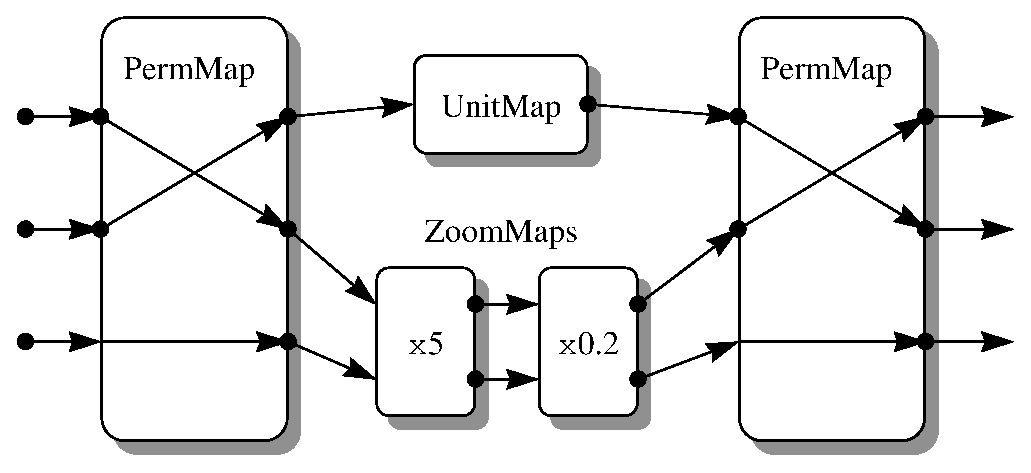
\includegraphics[scale=0.65]{sun210_figures/simpexamp.eps}
   \caption{An over-complex compound \htmlref{Mapping}{Mapping}, consisting of PermMaps,
   ZoomMaps and a \htmlref{UnitMap}{UnitMap}, which can be simplified to become a single
   UnitMap.  The enclosing nested CmpMaps have been omitted for clarity.}
   \label{fig:simplifyexample}
   \end{center}
   \end{figure}
\end{latexonly}
\begin{htmlonly}
   To illustrate how AST\_SIMPLIFY works, consider the combination of
   Mappings shown in the Figure below.
   \begin{quote}
   \begin{figure}
   \label{fig:simplifyexample}
   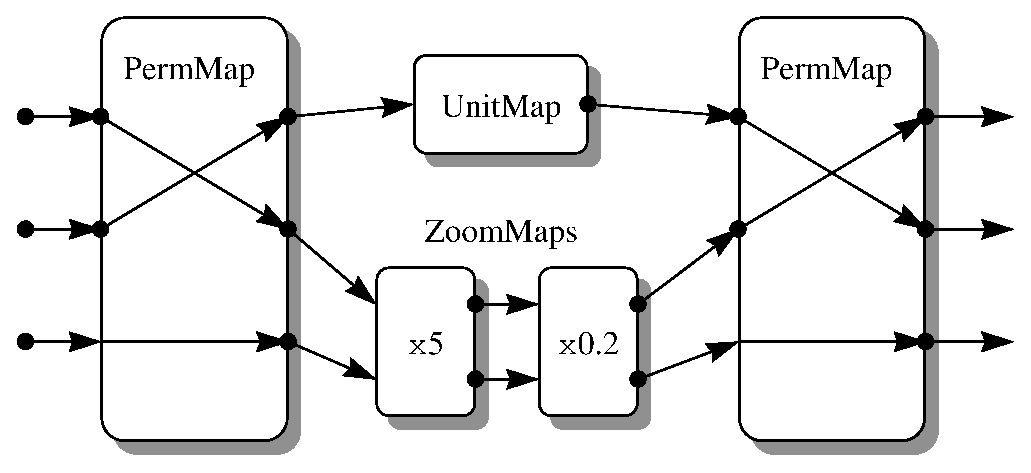
\includegraphics[scale=1.1]{sun210_figures/simpexamp.eps}
   \caption{An over-complex compound Mapping, consisting of PermMaps,
   ZoomMaps and a UnitMap, which can be simplified to become a single
   UnitMap.  The enclosing nested CmpMaps have been omitted for clarity.}
   \end{figure}
   \end{quote}
\end{htmlonly}
If this were contained in a CmpMap, it could be simplified as follows:

\small
\begin{verbatim}
      INTEGER SIMPLER

      ...

      SIMPLER = AST_SIMPLIFY( CMPMAP, STATUS );
\end{verbatim}
\normalsize

In this case, the result would be a simple 3-dimensional UnitMap (the
identity Mapping).  To reach this conclusion, AST\_SIMPLIFY will have
made a number of deductions, roughly as follows:

\begin{enumerate}
\item The two 2-dimensional ZoomMaps in series are equivalent to a
single \htmlref{ZoomMap}{ZoomMap} with a combined \htmlref{Zoom}{Zoom} factor of unity. This, in turn, is
equivalent to a 2-dimensional UnitMap.

\item This UnitMap in parallel with the other 1-dimensional UnitMap is
equivalent to a single 3-dimensional UnitMap. This UnitMap, sandwiched
between any other pair of Mappings, can then be eliminated.

\item The remaining two PermMaps in series are equivalent to a single
3-dimensional \htmlref{PermMap}{PermMap}. When these are combined, the resulting PermMap
is found to be equivalent to a 3-dimensional UnitMap.
\end{enumerate}

This example is a little contrived, but illustrates how AST\_SIMPLIFY
can deal with even quite complicated compound Mappings through a
series of incremental simplifications. Where possible, this will
result in either a simpler compound Mapping or, if feasible, an atomic
(non-compound) Mapping, as here. If no simplification is possible,
AST\_SIMPLIFY will just return a pointer to the original Mapping.

Although AST\_SIMPLIFY cannot identify every simplification that is
theoretically possible, sufficient rules are included to deal with the
most common and important cases.

\cleardoublepage
\section{\label{ss:frames}Representing Coordinate Systems (Frames)}

An AST \htmlref{Frame}{Frame} is an \htmlref{Object}{Object} that is used to represent a coordinate
system. Contrast this with a \htmlref{Mapping}{Mapping} (\secref{ss:mappings}), which is
used to describe how to convert between coordinate systems. The two
concepts are complementary and we will see how they work together in
\secref{ss:framesets}.

In this section we will discuss only basic Frames, which represent
Cartesian coordinate systems. More specialised types of Frame
({\em{e.g.}}\ the \htmlref{SkyFrame}{SkyFrame}, which represents celestial coordinate
systems, and the \htmlref{SpecFrame}{SpecFrame}, which represents spectral coordinate
systems) are covered later (\secref{ss:skyframes} and \secref{ss:specframes})
and, naturally, inherit the properties and behaviour of the simple Frames
discussed here.

\subsection{The Frame Model}

The best way to think about a \htmlref{Frame}{Frame} is like the frame that you would
plot around a graph. In two dimensions, you would have an ``$x$'' and
a ``$y$'' axis, a title on the graph and labels on the axes, together
with an indication of the physical units being plotted. The values
marked along each axis would be formatted in a human-readable way. The
frame around a graph therefore defines a coordinate space within which
you can locate points, draw lines, calculate distances, {\em{etc.}}

An AST Frame works in much the same way, embodying all of these
concepts and a few more. It also allows any number of axes, which
means that a Frame can represent coordinate systems with any number of
dimensions. You specify how many when you create it.

Remember that the basic Frame we are considering here is completely
general.  It knows nothing of celestial coordinates, for example, and
all its axes are equivalent. It can be adapted to describe any general
purpose Cartesian coordinate system by setting its attributes, such as
its \htmlref{Title}{Title} and axis Labels, {\em{etc.}}\ to appropriate values.

\subsection{\label{ss:creatingframes}Creating a Frame}

Creating a \htmlref{Frame}{Frame} is straightforward and follows the usual pattern:

\small
\begin{verbatim}
      INCLUDE 'AST_PAR'
      INTEGER FRAME, STATUS

      STATUS = 0

      ...

      FRAME = AST_FRAME( 2, ' ', STATUS )
\end{verbatim}
\normalsize

The first argument of the \htmlref{AST\_FRAME}{AST_FRAME} constructor function specifies
the number of axes which the Frame should have.

\subsection{\label{ss:frameasmapping}Using a Frame as a Mapping}

We should briefly point out that the \htmlref{Frame}{Frame} we created above
(\secref{ss:creatingframes}) is also a \htmlref{Mapping}{Mapping}
(\secref{ss:mappingclass}) and therefore inherits the properties and
behaviour common to other Mappings.

One way to see this is to set the Frame's \htmlref{Report}{Report} attribute (inherited
from the Mapping class) to a non-zero value and pass the Frame pointer
to a coordinate transformation routine, such as \htmlref{AST\_TRAN2}{AST_TRAN2}.

\small
\begin{verbatim}
      DOUBLE PRECISION XIN( 5 ), YIN( 5 ), XOUT( 5 ), YOUT( 5 )
      DATA XIN / 0D0, 1D0, 2D0, 3D0, 4D0, 5D0 /
      DATA YIN / 0D0, 2D0, 4D0, 6D0, 8D0, 10D0 /

      CALL AST_SET( FRAME, 'Report=1', STATUS )
      CALL AST_TRAN2( FRAME, 5, XIN, YIN, .TRUE., XOUT, YOUT, STATUS )
\end{verbatim}
\normalsize

The resulting output might then look like this:

\begin{quote}
\begin{verbatim}
(1, 2) --> (1, 2)
(2, 4) --> (2, 4)
(3, 6) --> (3, 6)
(4, 8) --> (4, 8)
(5, 10) --> (5, 10)
\end{verbatim}
\end{quote}

This is not very exciting because a Frame implements an identity
transformation just like a \htmlref{UnitMap}{UnitMap}
(\secref{ss:unitmapexample}). However, it illustrates that a Frame can
be used as a Mapping and that its \htmlref{Nin}{Nin} and \htmlref{Nout}{Nout} attributes are both
equal to the number of Frame axes.

When we consider more specialised Frames
({\em{e.g.}}~\secref{ss:framesets}), we will see that using them as
Mappings can be very useful indeed.

\subsection{\label{ss:frameaxisattributes}Frame Axis Attributes}

Frames have a number of attributes which can take multiple values, one
for each axis. These separate values are identified by appending the
axis number in parentheses to the attribute name. For example, the
Label(1) attribute is a character string containing the label which
appears on the first axis.

\htmlref{Axis}{Axis} attributes are accessed in the same way as all other attributes
(\secref{ss:gettingattributes}, \secref{ss:settingattributes} and
\secref{ss:defaultingattributes}). For example, the Label on the second
axis might be obtained as follows:

\small
\begin{verbatim}
      CHARACTER * ( 70 ) LABEL

      ...

      LABEL = AST_GETC( FRAME, 'Label(2)', STATUS )
\end{verbatim}
\normalsize

Other attribute access routines (AST\_SETx, \htmlref{AST\_TEST}{AST_TEST} and \htmlref{AST\_CLEAR}{AST_CLEAR})
may also be applied to axis attributes in the same way.

If the axis number is stored in a program variable, then its value
must be formatted to generate a suitable attribute name before using
this to access the attribute itself. For example, the following will
print out the Label value for each axis of a \htmlref{Frame}{Frame}:

\small
\begin{verbatim}
      CHARACTER * ( 10 ) AXIS
      INTEGER IAXIS

      ...

      DO 1 IAXIS = 1, AST_GETI( FRAME, 'Naxes', STATUS )
         WRITE ( AXIS, '( I10 )' ) IAXIS
         LABEL = AST_GETC( FRAME, 'Label(' // AXIS // ')', STATUS )
         WRITE ( *, 199 ) IAXIS, LABEL
 199     FORMAT ( 'Label ', I2, ': ', A )
 1    CONTINUE
\end{verbatim}
\normalsize

Note the use of the \htmlref{Naxes}{Naxes} attribute to determine the number of Frame
axes.

The output from this might look like the following:

\begin{quote}
\begin{verbatim}
Label  1: Axis 1
Label  2: Axis 2
\end{verbatim}
\end{quote}

In this case, the Frame's default axis Labels have been revealed as
rather un-exciting. Normally, you would set much more useful values,
typically when you create the Frame---perhaps something like:

\small
\begin{verbatim}
      FRAME = AST_FRAME( 2, 'Label(1)=Offset from centre of field,' //
                            'Unit(1) =mm,' //
                            'Label(2)=Transmission coefficient,' //
                            'Unit(2) =%', STATUS )
\end{verbatim}
\normalsize

Here, we have also set the (character string) Unit attribute for each
axis to describe the physical units represented on that axis. All the
attribute assignments have been combined into a single string,
separated by commas.

\subsection{\label{ss:frameattributes}Frame Attributes}

We will now briefly outline the various attributes associated with a
\htmlref{Frame}{Frame} (this is, of course, in addition to those inherited from the
\htmlref{Mapping}{Mapping} class). We will not delve too deeply into the details of each
attribute, for which you should consult the appropriate description in
\appref{ss:attributedescriptions}. Instead, we aim simply to sketch
the range of facilities available:

\begin{quote}
\begin{description}
\item[\htmlref{Naxes}{Naxes}]\mbox{}\\
A read-only integer giving the number of Frame axes.

\item[\htmlref{Title}{Title}]\mbox{}\\
A string describing the coordinate system which the Frame represents.

\item[\htmlref{Label(axis)}{Labelaxis}]\mbox{}\\
A label string for each axis.

\item[\htmlref{Unit(axis)}{Unitaxis}]\mbox{}\\
A string describing the physical units on each axis. You can choose
whether to make this attribute ``active'' or ``passive'' (using
\htmlref{AST\_SETACTIVEUNIT}{AST_SETACTIVEUNIT}
). If active, its value will be taken into account when finding the
Mapping between two Frames (\emph{e.g.} a scaling of 0.001 would be used
to connect two axis with units of ``km'' and ``m''). If passive, its value
is ignored. Its use is described in more detail in \secref{ss:frameunits}.

\item[\htmlref{Symbol(axis)}{Symbolaxis}]\mbox{}\\
A string containing a ``short form'' symbol ({\em{e.g.}}\ like ``X''
or ``Y'') used to represent the quantity plotted on each axis.

\item[\htmlref{Digits/Digits(axis)}{DigitsDigitsaxis}]\mbox{}\\
The preferred number of digits of precision to be used when formatting
values for display on each axis.

\item[\htmlref{Format(axis)}{Formataxis}]\mbox{}\\
A string containing a {\em{format specifier}} which determines exactly
how values should be formatted for display on each axis
(\secref{ss:formattingaxisvalues}). If this attribute is un-set, the
formatting is based on the Digits value, otherwise the Format string
over-rides the Digits value.

\item[\htmlref{Direction(axis)}{Directionaxis}]\mbox{}\\
A boolean (integer) value which indicates in which direction each axis
should be plotted. If it is non-zero (the default), the axis should be
plotted in the conventional direction---{\em{i.e.}}\ increasing to the
right for the abscissa and increasing upwards for the ordinate. If it
is zero, the axis should be plotted in reverse.  This attribute is
provided as a hint only and programs are free to ignore it if they
wish.

\item[\htmlref{Domain}{Domain}]\mbox{}\\
A character string which identifies the {\em{physical domain}} to
which the Frame's coordinate system applies. The primary purpose of
this attribute is to prevent unwanted conversions from occurring
between coordinate systems which are not related. Its use is described
in more detail in \secref{ss:framedomains}.

\item[\htmlref{System}{System}]\mbox{}\\
A character string which identifies the specific coordinate system used
to describe positions within the physical domain represented by the Frame.
For a simple Frame, this attribute currently has a fixed value of
``Cartesian'', but could in principle be extended to include options such
as ``Polar'', ``Cylindrical'', {\em{etc}}. More specialised Frames such
as the \htmlref{SkyFrame}{SkyFrame}, \htmlref{TimeFrame}{TimeFrame}  and \htmlref{SpecFrame}{SpecFrame}, re-define the allowed values to be
appropriate to the domain which they describe. For instance, the SkyFrame
allows values such as ``FK4'' and ``Galactic'', and the SpecFrame allows
values such as ``frequency'' and ``wavelength''.

\item[\htmlref{Epoch}{Epoch}]\mbox{}\\
This value is used to qualify a coordinate system by giving the moment in
time when the coordinates are correct. Usually, this will be the date of
observation. The Epoch value is important in cases where coordinates
systems move with respect to each other over time. An example of two such
coordinate systems are the FK4 and FK5 celestial coordinate systems.

\item[\htmlref{ObsLon}{ObsLon}]\mbox{}\\
Specifies the longitude of the observer (assumed to be on the surface of
the earth). The basic Frame class does not use this value, but
specialised sub-classes may. For instance, the SpecFrame class uses it to
calculate the relative velocity of the observer and the centre of the
earth for use in converting between standards of rest.

\item[\htmlref{ObsLat}{ObsLat}]\mbox{}\\
Specifies the latitude of the observer. Use in conjunction with ObsLon.

\end{description}
\end{quote}

There are also some further Frame attributes, not described above,
which are important when Frames are used as templates to search for
other Frames. Their use goes beyond the present discussion.
%TBW---Add reference here.

\subsection{\label{ss:formattingaxisvalues}Formatting Axis Values}

The coordinate values associated with each axis of a \htmlref{Frame}{Frame} are stored
({\em{e.g.}}\ within your program) as double precision values. The
Frame class therefore provides a function, \htmlref{AST\_FORMAT}{AST_FORMAT}, to convert
these values into formatted strings for display:

\small
\begin{verbatim}
      CHARACTER * ( 50 ) STRING
      DOUBLE PRECISION VALUE

      ...

      STRING = AST_FORMAT( FRAME, IAXIS, VALUE, STATUS )
\end{verbatim}
\normalsize

Here, the AST\_FORMAT character function is passed a Frame pointer,
the number of an axis (IAXIS) and a double precision value to format
(VALUE). It returns a character string containing the formatted value.
\label{ss:formattingwithdigits}

By default, the formatting applied will be determined by the Frame's
Digits attribute and will normally display results with seven digits
of precision (corresponding approximately to the Fortran REAL data
type on many machines). Setting a different Digits value, however,
allows you to adjust the precision as necessary to suit the accuracy
of the coordinate data you are processing.  If finer control is
needed, it is also possible to set a Digits value for each individual
axis by appending an axis number to the attribute name
({\em{e.g.}}\ ``Digits(2)''). If this is done, it over-rides the
effect of the Frame's main Digits value for that axis.

Even finer control is possible by setting the (character string)
Format attribute for a Frame axis. The string given should contain a
{\em{format specifier}} which explicitly determines how the values on
that axis should be formatted. This will over-ride the effects of any
Digits value\footnote{The exception to this rule is that if the Format value
includes a precision of ``$.*$'', then Digits will be used to determine
the actual precision used.}.  Unfortunately for Fortran programmers, this must
be a C language format specifier,\footnote{This is a consequence of
implementing the AST library in C.} so you might find the Digits
approach preferable.

The simplest type of format specifier takes the form ``\%m.nG'', where
``m'' and ``n'' are integers giving the minimum field width in characters
and the number of significant digits to display ({\em{e.g.}}\
``\%10.5G''). The ''n'' value may be replaced by an asterisk, in which
case the value of the Digits attribute is used to determine the number of
significant digits to display. Other formatting options are also possible
and if you need to use them you may wish to consult a book on C (see the
``printf'' function), remembering that you want to format a double
precision (C double) value.

It is recommended that you use AST\_FORMAT whenever you display
formatted coordinate values, even although you could format them
yourself using a WRITE statement. This is because it puts the Frame in
control of formatting. When you start to handle more elaborate Frames
(representing, say, celestial coordinates), you will need different
formatting methods. This approach delivers them without any change to
your software.

You should also consider regularly using the \htmlref{AST\_NORM}{AST_NORM} routine,
described below (\secref{ss:normalising}), for any values that will be
made visible to the user of your software.

\subsection{\label{ss:normalising}Normalising Frame Coordinates}

The routine \htmlref{AST\_NORM}{AST_NORM} is provided to cope with the fact that some
coordinate systems do not extend indefinitely in all directions. Some
may have boundaries, outside which coordinates are meaningless, while
others wrap around on themselves, so that after a certain distance you
return to the beginning again (coordinate systems based on circles and
spheres, for instance). A basic \htmlref{Frame}{Frame} has no such complications, but
other more specialised Frames (such as SkyFrames, representing the
celestial sphere---\secref{ss:skyframes}) do.

The role played by AST\_NORM is to {\em{normalise}} any arbitrary set
of coordinates by converting them into a set which is ``within
bounds'', interpreted according to the particular Frame in
question. For example, on the celestial sphere, a right ascension
value of 24~hours or more can have a suitable multiple of 24~hours
subtracted without affecting its meaning and AST\_NORM would perform
this task. Similarly, negative values of right ascension would have a
multiple of 24~hours added, so that the result lies in the range zero
to 24~hours. The coordinates in question are modified in place by
AST\_NORM, as follows:

\small
\begin{verbatim}
      DOUBLE PRECISION POINT( 2 )

      ...

      CALL AST_NORM( FRAME, POINT, STATUS )
\end{verbatim}
\normalsize

If the coordinates supplied are initially OK, as they would always be
with a basic Frame, then they are returned unchanged.

Because the main purpose of AST\_NORM is to convert coordinates into
the preferred range for human consumption, its use is almost always
appropriate immediately before formatting coordinate values for
display using \htmlref{AST\_FORMAT}{AST_FORMAT} (\secref{ss:formattingaxisvalues}). Even if
the Frame in question does not restrict the range of coordinates, so
that AST\_NORM does nothing, using it will allow you to process other
more specialised Frames, where normalisation is important, without
changing your software.

\subsection{\label{ss:unformattingaxisvalues}Reading Formatted Axis Values}

The process of converting a formatted coordinate value for a \htmlref{Frame}{Frame}
axis, such as might be produced by \htmlref{AST\_FORMAT}{AST_FORMAT}
(\secref{ss:formattingaxisvalues}), back into a numerical (double
precision) value ready for processing is performed by \htmlref{AST\_UNFORMAT}{AST_UNFORMAT}.
However, although this process is essentially the inverse of that
performed by AST\_FORMAT, there are a number of additional difficulties
that must be addressed in practice.

The main use for AST\_UNFORMAT is in reading formatted coordinate
values which have been entered by the user of a program, or read from
a file. As such, we can rarely assume that the values are neatly
formatted in the way that AST\_FORMAT would produce. Instead, it is
usually desirable to allow considerable flexibility in the form of
input that can be accommodated, so as to permit ``free-format'' data
input by the user. In addition, we may need to extract individual
coordinate values embedded in other textual data.

Underlying these requirements is the root difficulty that the textual
format used to represent a coordinate value will depend on the class
of Frame we are considering. For example, for a basic Frame,
AST\_UNFORMAT may have to read a value like ``1.25E-6'', whereas a
more specialised Frame representing celestial coordinates may have to
handle a value like ``-07d~49m~13s''. Of course, the format might also
depend on which axis is being considered.

Ideally, we would like to write software that can handle any kind of
Frame. However, this makes it a little more difficult to analyse
textual input data to extract individual coordinate values, since we
cannot make assumptions about how the values are formatted. It would
not be safe, for example, simply to assume that the values being read
are separated by white space. This is not just because they might be
separated by some other character, but also because celestial
coordinate values might themselves contain spaces. In fact, to be
completely safe, we cannot make any assumptions about how a formatted
coordinate value is separated from the surrounding text, except that
it should be separated in some way which is not ambiguous.

This is the very basic assumption upon which AST\_UNFORMAT works. It is
invoked as follows:

\small
\begin{verbatim}
      INTEGER N

      ...

      N = AST_UNFORMAT( FRAME, IAXIS, STRING, VALUE, STATUS )
\end{verbatim}
\normalsize

It is supplied with a Frame pointer (FRAME), the number of an axis
(IAXIS) and a character string to be read (STRING). If it succeeds in
reading a value, AST\_UNFORMAT returns the resulting coordinate
{\em{via}} its penultimate argument (VALUE). The returned function
value indicates how many characters were read from the string in order
to obtain this result.

The string is read as follows:

\begin{enumerate}
\item Any white space at the start is skipped over.

\item Further characters are considered, one at a time, until the next
character no longer matches any of the acceptable forms of input
(given the characters that precede it). The longest sequence of
characters which matches is then considered ``read''.

\item If a suitable sequence of characters was read successfully, it
is converted into a coordinate value which is returned. Any white
space following this sequence is then skipped over and the total
number of characters consumed is returned as the function value.

\item If the sequence of characters read is empty, or insufficient to
define a coordinate value, then the string does not contain a value to
read. In this case, the read is aborted and AST\_UNFORMAT returns a
function value of zero and no coordinate value. However, it returns
without error.
\end{enumerate}

Note that failing to read a coordinate value does not constitute an
error, at least so far as AST\_UNFORMAT is concerned. However, an
error can occur if the sequence of characters read appears to have the
correct form but cannot be converted into a valid coordinate
value. Typically, this will be because it violates some constraint,
such as a limit on the value of one of its fields. The resulting error
message will give details.

For any given Frame axis, AST\_UNFORMAT does not necessarily always
use the same algorithm for converting the sequence of characters it
reads into a coordinate value. This is because some forms of input
(particularly free-format input) can be ambiguous and might be
interpreted in several ways depending on the context. For example, the
celestial longitude ``12:34:56.7'' could represent an angle in degrees
or a right ascension in hours. To decide which to use, AST\_UNFORMAT
may examine the Frame's attributes and, in particular, the appropriate
\htmlref{Format(axis)}{Formataxis} string which is used by AST\_FORMAT when formatting
coordinate values (\secref{ss:formattingaxisvalues}). This is done in
order that AST\_FORMAT and AST\_UNFORMAT should complement each
other---so that formatting a value and then un-formatting it will
yield the original value, subject to any rounding error.

To give a simple (but crucially incomplete!) example, consider reading
a value for the axis of a basic Frame, as follows:

\small
\begin{verbatim}
      N = AST_UNFORMAT( FRAME, IAXIS, ' 1.5E6   -99.0', VALUE, STATUS )
\end{verbatim}
\normalsize

AST\_UNFORMAT will skip over the initial space in the string supplied
and then examine each successive character. It will accept the
sequence ``1.5E6'' as input, but reject the space which follows
because it does not form part of the format of a floating point
number. It will then convert the characters ``1.5E6'' into a
coordinate value and skip over the three spaces which follow them. The
returned function value will therefore be 9, equal to the total number
of characters consumed. This result may be used to address the string
during a subsequent read, so as to commence reading at the start of
``-99.0''.

Most importantly, however, note that if the user of a program
mistakenly enters the string ``~1.5R6\ldots'' instead of
``~1.5E6\ldots'', a coordinate value of 1.5 and a function result of 4
will be returned, because the ``R'' would prematurely terminate the
attempt to read the value. Because this sort of mistake does not
automatically result in an error but can produce incorrect results, it
is {\bf{vital}} to check the returned function value to ensure that
the expected number of characters have been read. For example, if the
string is expected to contain exactly one value, and nothing else,
then the following would suffice:

\small
\begin{verbatim}
      N = AST_UNFORMAT( FRAME, IAXIS, STRING, VALUE, STATUS )
      IF ( STATUS .EQ. 0 ) THEN
         IF ( N .LT. LEN( STRING ) ) THEN
            <error in input data>
         ELSE
            <value read correctly>
         END IF
      END IF
\end{verbatim}
\normalsize

If AST\_UNFORMAT does not detect an error itself, we check that it has
read to the end of the string. If this reveals an error, the value of
N indicates where it occurred.

Another common requirement is to obtain a position by reading a list
of coordinates from a string which contains one value for each axis of
a Frame. We assume that the values are separated in some unambiguous
manner, perhaps using white space and/or some unspecified
single-character separator. The choice of separator is up to the data
supplier, who must choose it so as not to conflict with the format of
the coordinate values, but our software does not need to know what it
is. The following is a template algorithm for reading data in this
form:

\small
\begin{verbatim}
      INTEGER I
      DOUBLE PRECISION VALUES( 10 )

      ...

*  Initialise the string index.
      I = 1

*  Obtain the number of Frame axes and loop through them.
      DO 1 IAXIS = 1, AST_GETI( FRAME, 'Naxes', STATUS )

*  Attempt to read a value for this axis.
         N = AST_UNFORMAT( FRAME, IAXIS, STRING( I : ),
     :                     VALUES( IAXIS ), STATUS )

*  If nothing was read and this is not the first axis and the end of
*  the string has not been reached, try stepping over a separator and
*  reading again.
         IF ( ( N .EQ. 0 ) .AND. ( IAXIS .GT. 1 ) .AND.
     :        ( I .LT. LEN( STRING ) ) ) THEN
            I = I + 1
            N = AST_UNFORMAT( FRAME, IAXIS, STRING( I : ),
     :                        VALUES( IAXIS ), STATUS )
         END IF

*  Quit if nothing was read, otherwise move on to the next value.
         IF ( N .EQ. 0 ) GO TO 2
         I = I + N
 1    CONTINUE
 2    CONTINUE

*  Check for possible errors.
      IF ( STATUS .EQ. 0 ) THEN
         IF ( ( I .LT. LEN( STRING ) ) .OR. ( N .EQ. 0 ) ) THEN
            <error in input data>
         ELSE
            <values read correctly>
         END IF
      END IF
\end{verbatim}
\normalsize

In this case, the value of I will indicate the location of any input error.

Note that this algorithm is insensitive to the precise format of the
data and will therefore work with any class of Frame and any
reasonably unambiguous input data. For example, here is a range of
suitable input data for a 3-dimensional basic Frame:

\begin{quote}
\small
\begin{verbatim}
1 2.5 3
3.1,3.2,3.3
1.5, 2.6, -9.9e2
-1.1+0.4-1.8
    .1/.2/.3
 44.0 ; 55.1 -14
\end{verbatim}
\normalsize
\end{quote}

\subsection{\label{ss:permutingaxes}Permuting Frame Axes}

Once a \htmlref{Frame}{Frame} has been created, it is not possible to change the number
of axes it contains, but it is possible to change the order in which
these axes occur. To do so, an integer {\em{permutation array}} is
filled with the numbers of the axes so as to specify the new order,
{\em{e.g:}}

\small
\begin{verbatim}
      INTEGER PERM( 2 )
      DATA PERM / 2, 1 /
\end{verbatim}
\normalsize

In this case, the axes of a 2-dimensional Frame could be interchanged
by passing this permutation array to the \htmlref{AST\_PERMAXES}{AST_PERMAXES} function. That
is, an ($x_1,x_2$) coordinate system would be changed into an
($x_2,x_1$) coordinate system by:

\small
\begin{verbatim}
      CALL AST_PERMAXES( FRAME, PERM, STATUS )
\end{verbatim}
\normalsize

If the axes are permuted more than once, the effects are cumulative.
You are, of course, not restricted to Frames with only two axes.

\subsection{Selecting Frame Axes}

An alternative to changing the number of \htmlref{Frame}{Frame} axes, which is not
allowed, is to create a new Frame by selecting axes from an existing
one. The method of doing this is very similar to the way \htmlref{AST\_PERMAXES}{AST_PERMAXES}
is used (\secref{ss:permutingaxes}), in that we supply an integer
array filled with the numbers of the axes we want, in their new
order. In this case, however, the number of array elements need not
equal the number of Frame axes.

For example, we could select axes 3 and 2 (in that order) from a
3-dimensional Frame as follows:

\small
\begin{verbatim}
      INTEGER FRAME1, FRAME2, MAPPING, PICK( 2 )
      DATA PICK / 3, 2 /

      ...

      FRAME2 = AST_PICKAXES( FRAME1, 2, PICK, MAPPING, STATUS )
\end{verbatim}
\normalsize

This would return a pointer to a 2-dimensional Frame (FRAME2) which
contains the information associated with axes 3 and 2, in that order,
from the original Frame (FRAME1). The original Frame is not altered by
this process. Beware, however, that the axis information may still be
shared by both Frames, so if you wish to alter either of them
independently you may first need to use \htmlref{AST\_COPY}{AST_COPY}
(\secref{ss:copyingobjects}) to make an independent copy.

In addition to the new Frame pointer, \htmlref{AST\_PICKAXES}{AST_PICKAXES} will also return a
pointer to a new \htmlref{Mapping}{Mapping} {\em{via}} its fourth argument. This Mapping will
inter-relate the two Frames. By this we mean that its forward
transformation will convert coordinates originally in the coordinate
system represented by FRAME1 into that represented by FRAME2, while
its inverse transformation will convert in the opposite direction. In
this particular case, the Mapping would be a \htmlref{PermMap}{PermMap}
(\secref{ss:permmapexample}) and would implement the following
transformations:

\begin{quote}
\begin{verbatim}
Forward:
   (1, 2, 3) --> (3, 2)
   (2, 4, 6) --> (6, 4)
   (3, 6, 9) --> (9, 6)
   (4, 8, 12) --> (12, 8)
   (5, 10, 15) --> (15, 10)

Inverse:
   (3, 2) --> (<bad>, 2, 3)
   (6, 4) --> (<bad>, 4, 6)
   (9, 6) --> (<bad>, 6, 9)
   (12, 8) --> (<bad>, 8, 12)
   (15, 10) --> (<bad>, 10, 15)
\end{verbatim}
\end{quote}

This is our first introduction to the idea of inter-relating pairs of
Frames {\em{via}} a Mapping, but this will assume a central role later on.

Note that when using AST\_PICKAXES, it is also possible to request
more axes than there were in the original Frame. This will involve
selecting axes from the original Frame that do not exist. To do this,
the corresponding axis number (in the PICK array) should be set to
zero and the effect is to introduce an additional new axis which is
not derived from the original Frame. This axis will have default
values for all its attributes. You will need to do this because
AST\_PICKAXES does not allow you to select any of the original axes
more than once.\footnote{It will probably not be obvious why this
restriction is necessary, but consider creating a Frame with one
longitude axis and two latitude axes. Which latitude axis should be
associated with the longitude axis?}

\subsection{\label{ss:distanceandoffset}Calculating Distances, Angles and Offsets}
Some complementary
routines
are provided for use with Frames to allow you to perform geometric
operations without needing to know the nature of the coordinate system
represented by the \htmlref{Frame}{Frame}.

Routines
can be used to find the distance between two points, and to offset a
specified distance along a line joining two points, {\em{etc.}} In essence,
these define the metric of the coordinate space which the Frame represents. In
the case of a basic Frame, this is a Cartesian metric.

The first of these routines, \htmlref{AST\_DISTANCE}{AST_DISTANCE}, returns a double precision
distance value when supplied with the Frame coordinates of two
points. For example:

\small
\begin{verbatim}
      DOUBLE PRECISION DIST, POINT1( 2 ), POINT2( 2 )
      DATA POINT1 / 0D0, 0D0 /
      DATA POINT2 / 1D0, 1D0 /

      ...

      DIST = AST_DISTANCE( FRAME, POINT1, POINT2, STATUS )
\end{verbatim}
\normalsize

This calculates the distance between the origin (0,0) and a point at
position (1,1). In this case, the result, as you would expect, is
$\surd{2}$. However, this is only true for the Cartesian coordinate
system which a basic Frame represents. In general, AST\_DISTANCE will
calculate the geodesic distance between the two points, so that with a
more specialised Frame (such as a \htmlref{SkyFrame}{SkyFrame}, representing the celestial
sphere) a great-circle distance might be returned.

The \htmlref{AST\_OFFSET}{AST_OFFSET} routine is really the inverse of AST\_DISTANCE. Given
two points in a Frame, it calculates the coordinates of a third point
which is offset a specified distance away from the first point along
the geodesic joining it to the second one. For example:

\small
\begin{verbatim}
      DOUBLE PRECISION POINT1( 2 ), POINT2( 2 ), POINT3( 2 )
      DATA POINT1 / 0D0, 0D0 /
      DATA POINT2 / 1D0, 1D0 /

      ...

      CALL AST_OFFSET( FRAME, POINT1, POINT2, 0.5D0, POINT3, STATUS )
\end{verbatim}
\normalsize

This would fill the POINT3 array with the coordinates of a point which
is offset 0.5 units away from the origin (0,0) in the direction of the
position (1,1). Again, this is a simple result in a Cartesian Frame,
as varying the offset will trace out a straight line. On the celestial
sphere, however ({\em{e.g.}}\ using a SkyFrame), it would trace out a
great circle.

The routines \htmlref{AST\_AXDISTANCE}{AST_AXDISTANCE} and \htmlref{AST\_AXOFFSET}{AST_AXOFFSET} are similar to AST\_DISTANCE
and AST\_OFFSET, except that the curves which they use as ``straight
lines'' are not geodesics, but curves parallel to a specified axis\footnote
{For instance, a line of constant Declination is not a geodesic}. One
reason for using these routines is to deal with the cyclic ambiguity of
longitude and latitude axes.

The \htmlref{AST\_OFFSET2}{AST_OFFSET2} routine is similar to AST\_OFFSET, but instead of using the
geodesic which passes through two positions, it uses the geodesic which
passes at a given position angle through the starting position.

Position angles are always measured from the positive direction of the
second Frame axis to the required line, with positive angles being in the
same sense as rotation from the positive direction of the second axis to
the positive direction of the first Frame axis. This definition applies
to all classes of Frame, including SkyFrame. The default ordering of axes
in a SkyFrame makes the second axis equivalent to north, and so the
definition of position angle given above corresponds to the normal
astronomical usage, ``from north, through east''. However, it should be
remembered that it is possible to permute the axes of a SkyFrame (or
indeed any Frame), so that north becomes axis 1. In this case, an AST
``position angle'' would be the angle ``from east, through north''.
Always take the axis ordering into account when deriving an astronomical
position angle from an AST position angle.

Within a Cartesian coordinate system, the position angle of a geodesic
({\em{i.e.}}\ a straight line) is constant along its entire length, but
this is not necessarily true of other coordinate systems. Within a
spherical coordinate system, for instance, the position angle of a geodesic
will vary along its length (except for the special cases of a meridian and
the equator). In addition to returning the required offset position, the
AST\_OFFSET2 routine
returns the position angle of the geodesic at the
offset position. This is useful if you want to trace out a path which
involves turning through specified angles. For instance, tracing out a
rectangle in which each side is a geodesic involves turning through 90
degrees at the corners. To do this, use AST\_OFFSET2 to calculate the
position of each corner, and then add (or subtract) 90 degrees from the
position angle returned by AST\_OFFSET2.

The \htmlref{AST\_ANGLE}{AST_ANGLE} routine
calculates the angle subtended by two points, at a third point.
If used with a 2-dimensional Frame the returned angle
is signed to indicate the sense of rotation (clockwise or anti-clockwise)
in taking the ``shortest route'' from the first point to the second.
If the Frame has more than 2 axes, the result is un-signed and is always
in the range zero to $\pi$.

The \htmlref{AST\_AXANGLE}{AST_AXANGLE} routine is similar to AST\_AXANGLE,
but the ``reference direction'', from which angles are measured, is
a specified axis.

The \htmlref{AST\_RESOLVE}{AST_RESOLVE} routine
resolves a given displacement within a Frame into two components, parallel and
perpendicular to a given reference direction.

The displacement is specified by two positions within the Frame; the
starting and ending positions. The reference direction is defined by the
geodesic curve passing through the starting position and a third specified
position. The lengths of the two components are returned, together with
the position on the reference geodesic which is closest to the third
supplied point.

\subsection{\label{ss:framedomains}The Domain Attribute}

The \htmlref{Domain}{Domain} attribute is one of the most important properties of a
\htmlref{Frame}{Frame}, although the concept it expresses can sometimes seem a little
subtle.  We will introduce it here, but its true value will probably
not become apparent until later (\secref{ss:framesetconverting}).

To understand the need for the Domain attribute, consider using
different Frames to represent the following different coordinate
systems associated with a CCD image:

\begin{enumerate}
\item A coordinate system based on pixel numbers.

\item Positions on the CCD chip, measured in $\mu$m.

\item Positions in the focal plane of the telescope, measured in mm.

\item A celestial coordinate system, measured in radians.
\end{enumerate}

If we had two such CCD images, we might legitimately want to align
them pixel-for-pixel ({\em{i.e.}}\ using the coordinate system based
on pixel numbers) in order to, say, divide by a flat-field exposure.
We might similarly consider aligning them using any of the other
coordinate systems so as to achieve different results. For example, we
might consider merging separate images from a CCD mosaic by using
focal plane positions.

It would obviously not be legitimate, however, to directly compare
positions in one image measured in pixels with positions in the other
measured in mm, nor to equate chip positions in $\mu$m with sky
coordinates in radians. If we wanted to inter-compare these
coordinates, we would need to do it indirectly, using other
information based on the experimental set-up. For instance, we might
need to know the size of the pixels expressed in mm and the
orientation of the CCD chip in the focal plane.

Note that it is not simply the difference in physical units which
prevents certain coordinates from being directly inter-compared
(because the appropriate unit scaling factors could be included
without any additional information). Neither is it the fact that
different coordinate systems are in use (because we could legitimately
inter-compare two different celestial coordinate systems without any
extra information).  Instead, it is the different nature of the
coordinate spaces to which these coordinate systems have been applied.

We normally express this by saying that the coordinate systems apply
to different {\em{physical domains}}. Although we may establish
{\em{ad hoc}} relationships between coordinates in different physical
domains, they are not intrinsically related to each other and we need
to supply extra information before we can convert coordinates between
them.

In AST, the role of the (character string) Domain attribute is to
assign Frames to their respective physical domains. The way it
operates is as follows:

\begin{itemize}
\item Coordinate systems which apply to the same physical domain
({\em{i.e.}}\ whose Frames have the same Domain value) can be directly
inter-compared.

If the domain has several coordinate systems associated with it
({\em{e.g.}}\ the celestial sphere), then a coordinate conversion may
be involved. Otherwise, coordinate values may simply be equated.

\item Coordinate systems which apply to different physical domains
({\em{i.e.}}\ whose Frames have different Domain values) cannot be
directly inter-compared.

If any relationship does exist between such coordinate systems---and
it need not---then additional information must be supplied in order to
establish the relationship between them in any particular case. We
will see later (\secref{ss:framesets}) how to establish such
relationships between Frames in different domains.
\end{itemize}

With the basic Frames we are considering here, each physical domain only
has a single (Cartesian) coordinate system associated with it, so that if
two such Frames have the same Domain value, their coordinate systems will
be identical and may simply be equated. With more specialised Frames,
however, more than one coordinate system may apply to each domain. In
such cases, a coordinate conversion may need to be performed.

When a basic Frame is created, its Domain attribute defaults to a
blank string. This means that all such Frames belong to the same
(null) domain by default and therefore describe the same unspecified
physical coordinate space. In order to assign a Frame to a different
domain, you simply need to set its Domain value. This is normally most
conveniently done when it is created, as follows:

\small
\begin{verbatim}
      FRAME1 = AST_FRAME( 2, 'Domain=CCD_CHIP,' //
                             'Unit(1)=micron,' //
                             'Unit(2)=micron', STATUS )
      FRAME2 = AST_FRAME( 2, 'Domain=FOCAL_PLANE,' //
                             'Unit(1)=mm,' //
                             'Unit(2)=mm', STATUS )
\end{verbatim}
\normalsize

Here, we have created two Frames in different physical
domains. Although their coordinate values all have units of length,
they cannot be directly inter-compared (because their axes may be
rotated with respect to each other, for instance).

All Domain values are automatically converted to upper case and white
space is removed, but there are no other restrictions on the names you
may use to label different physical domains. From a practical point of
view, however, it is worth following a few conventions
(\secref{ss:domainconventions}).

\subsection{\label{ss:domainconventions}Conventions for Domain Names}

When choosing a value for the \htmlref{Domain}{Domain} attribute of a \htmlref{Frame}{Frame}, it
obviously makes sense to avoid generic names which might clash with
those used for similar (but subtly different!) purposes by other
programmers. If you are developing software for an instrument, for
example, and want to identify an instrumental coordinate system, then
it is sensible to add a distinguishing prefix. For instance, you might
use $<$INST$>$\_FOCAL\_PLANE, where $<$INST$>$ ({\em{e.g.}}\ an
acronym) identifies your instrument.

For some purposes, however, a standard choice of Domain name is
desirable so that different items of software can communicate. For
this purpose, the following Domain names are reserved by AST and the
use recommended below should be carefully observed:

\begin{quote}
\begin{description}
\item[GRAPHICS]\mbox{}\\
Identifies the coordinate space used by an underlying computer
graphics system to specify plotting operations. Typically, when
performing graphical operations, AST is used to define additional
coordinate systems which are related to these ``native'' graphical
coordinates.  Plotting may be carried out in any of these coordinate
systems, but the GRAPHICS domain identifies the native coordinates
through which AST communicates with the underlying graphics system.

\item[GRID]\mbox{}\\
Identifies the instantaneous {\em{data grid}} used to store and handle
data, together with an associated coordinate system. In this
coordinate system, the first element stored in an array of data always
has a coordinate value of unity at its centre and all elements have
unit extent. This applies to all dimensions.

If data are copied or transformed to a new data grid (by whatever
means), or a subset of the original grid is extracted, then the same
rules apply to the copy or subset. Its first element therefore has
GRID coordinate values of unity at its centre. Note that this means
that GRID coordinates remain attached to the first element of the data
grid and not to its data content ({\em{e.g.}}\ the features in an
image).

\item[PIXEL]\mbox{}\\
Identifies an array of pixels and an associated {\em{pixel-based}}
coordinate system which is related to the GRID coordinate system
(above) simply by a shift of origin along each axis. This shift may be
integral, fractional, positive, negative or zero. The data elements
retain their unit extent along each axis.

Because the amount of shift is unspecified, the PIXEL domain is
distinct from the GRID domain. The relationship between them contains
a degree of uncertainty, such as typically arises from the different
conventions used by different software systems. For instance, in some
software the first pixel is regarded as being centred at (1,1), while
in other software it is at (0.5,0.5). In addition, some software
packages implement a ``pixel origin'' which allows pixel coordinates
to start at an arbitrary value.

The GRID domain (which corresponds with the pixel-numbering convention
used by FITS) is a special case of the PIXEL domain and avoids this
uncertainty. In general, additional information is required in order
to convert from one to the other.

\item[SKY]\mbox{}\\
Identifies the domain which contains all equivalent celestial
coordinate systems. Because these are represented in AST by SkyFrames
(\secref{ss:skyframes}), it should be no surprise that the default
Domain value for a \htmlref{SkyFrame}{SkyFrame} is SKY. Since there is only one sky, you
probably won't need to change this very often.

\item[SPECTRUM]\mbox{}\\
Identifies the domain used to describe positions within an
electro-magnetic spectrum. The AST \htmlref{SpecFrame}{SpecFrame} (\secref{ss:specframes})
class describes positions within this domain, allowing a wide range of
different coordinate systems to be used (frequency, wavelength,
{\em{etc}}). The default Domain value for a SpecFrame is SPECTRUM.

\item[TIME]\mbox{}\\
Identifies the domain used to describe moments in time. The AST \htmlref{TimeFrame}{TimeFrame}
class describes positions within this domain, allowing a wide range of
different coordinate systems and timescales to be used. The default Domain
value for a TimeFrame is TIME.

\end{description}
\end{quote}

Although we have drawn a necessary distinction here between the GRID
and PIXEL domains, we will continue to refer in general terms to image
``pixels'' and ``pixel coordinates'' whenever this distinction is not
important. This should not be taken to imply that the GRID convention
for numbering pixels is excluded---in fact, it is usually to be
preferred (at the level of data handling being discussed in this
document) and we recommend it.

\subsection{\label{ss:frameunits}The Unit Attribute}
Each axis of a \htmlref{Frame}{Frame} has a Unit attribute which holds the physical units used
to describe positions on the axis. The index of the axis to which the
attribute refers should normally be placed in parentheses following the
attribute name (``Unit(2)'' for instance). However, if the Frame has only
a single axis, then the axis index can be omitted.

In versions of AST prior to version 2.0, the Unit attribute was nothing
more than a descriptive string intended purely for human readers---no
part of the AST system used the Unit string for any purpose (other than
inclusion in axis labels produced by the \htmlref{Plot}{Plot} class). In particular, no
account was taken of the Unit attribute when finding the \htmlref{Mapping}{Mapping} between
two Frames. Thus if the conversion between a pair of 1-dimensional Frames
representing velocity was found (using
\htmlref{AST\_CONVERT}{AST_CONVERT}
) the returned Mapping would always be a \htmlref{UnitMap}{UnitMap}, even if the Unit
attributes of the two Frames were ``km/h'' and ``m/s''. This behaviour is
referred to below as a \emph{passive} Unit attribute.

As of AST version 2.0, a facility exists which allows the Unit attribute
to be \emph{active}; that is, differences in the
Unit attribute may be taken into account when finding the Mapping between
two Frames. In order to minimise the risk of breaking older software, the
\emph{default} behaviour of simple Frames and SkyFrames is unchanged from
previous versions (\emph{i.e.} they have passive Unit attributes). However,
the new
routines \htmlref{AST\_SETACTIVEUNIT}{AST_SETACTIVEUNIT} and \htmlref{AST\_GETACTIVEUNIT}{AST_GETACTIVEUNIT}
allow this default behaviour to be changed. The \htmlref{SpecFrame}{SpecFrame} and \htmlref{TimeFrame}{TimeFrame}
classes \emph{always} have an active Unit attribute (attempts to change this
are ignored).

For instance, consider the above example of two 1-dimensional Frames
describing velocity. These Frames can be created as follows:

\small
\begin{verbatim}
      INTEGER FRAME1, FRAME2

      FRAME1 = AST_FRAME( 1, 'Domain=VELOCITY,Unit=km/h' )
      FRAME2 = AST_FRAME( 1, 'Domain=VELOCITY,Unit=m/s' )

\end{verbatim}
\normalsize

By default, these Frames have passive Unit attributes, and so an attempt
to find a Mapping between them would ignore the difference in their Unit
attributes and return a unit Mapping. To avoid this, we indicate that we
want these Frames to have \emph{active} Unit attributes, as follows:

\small
\begin{verbatim}
      CALL AST_SETACTIVEUNIT( FRAME1, .TRUE., STATUS )
      CALL AST_SETACTIVEUNIT( FRAME2, .TRUE., STATUS )
\end{verbatim}
\normalsize

If we then find the Mapping between them as follows:

\small
\begin{verbatim}
      INTEGER CVT
      ...
      CVT = AST_CONVERT( FRAME1, FRAME2, ' ', STATUS )
\end{verbatim}
\normalsize

the Mapping contained within the \htmlref{FrameSet}{FrameSet} returned by
AST\_CONVERT
will be a one-dimensional \htmlref{ZoomMap}{ZoomMap} which simply scales its input (a
velocity in $km/h$) by a factor of 0.278 to create its output (a velocity
in $m/s$).

In fact we need not have set the Unit attribute active in FRAME1
since the behaviour of AST\_CONVERT is determined by its TO Frame
(the second Frame argument).

\subsubsection{\label{ss:unitsyntax}The Syntax for Unit Strings}
Conversion between units systems relies on the use of a specific syntax
for the Unit attribute. If the value of the Unit attribute does not
conform to this syntax, then an error will be reported if an attempt is
made to use it to determine an inter-unit \htmlref{Mapping}{Mapping} (this will never happen
if the Unit attribute is \emph{passive}).

The adopted syntax is that described in FITS-WCS paper I "Representation
of World Coordinate in FITS" by Greisen \& Calabretta. We distinguish
here between ``basic'' units and ``derived'' units: derived units are
defined in terms of other units (either derived or basic), whereas basic
units have no such definitions. Derived units may be represented by their
own \emph{symbol} (\emph{e.g.} ``Jy''---the Jansky) or by a
\emph{mathematical expression} which combines other symbols and constants
to form a definition of the unit (\emph{e.g.} ``km/s''---kilometres per
second). Unit symbols may be prefixed by a string representing a standard
multiple or sub-multiple.

In addition to the unit symbols listed in FITS-WCS Paper I, any other
arbitrary unit symbol may be used, with the proviso that it will not be
possible to convert between Frames using such units. The exception to
this is if both Frames refer to the same unknown unit string. For instance,
an axis with unknown unit symbol "flop" \emph{could} be converted to an axis
with  unit "Mflop" (Mega-flop).

Unit symbols (optionally prefixed with a multiple or sub-multiple) can be
combined together using a limited range of mathematical operators and
functions, to produce new units. Such expressions may also contain
parentheses and numerical constants (these may optionally use
``scientific'' notation including an ``E'' character to represent the
power of 10).

The following tables list the symbols for the basic and derived units which
may be included in a units string, the standard prefixes for multiples
and sub-multiples, and the strings which may be used to represent
mathematical operators and functions.

\begin{table}[htbp]
\begin{center}
\begin{tabular}{|l|l|l|}
\hline
\multicolumn{3}{|c|}{{\large Basic units}} \\ \hline
\multicolumn{1}{|c|}{Quantity} & \multicolumn{1}{|c|}{Symbol} &
\multicolumn{1}{c|}{\htmlref{Full}{Full} Name} \\ \hline
length              & m   & metre \\
mass                & g   & gram \\
time                & s   & second \\
plane angle         & rad & radian \\
solid angle         & sr  & steradian \\
temperature         & K   & Kelvin \\
electric current    & A   & Ampere \\
amount of substance & mol & mole \\
luminous intensity  & cd  & candela \\
\hline
\end{tabular}
\end{center}
\end{table}

\begin{table}[htbp]
\begin{center}
\begin{tabular}{|l|l|l|l|}
\hline
\multicolumn{4}{|c|}{{\large Derived units}} \\ \hline
\multicolumn{1}{|c|}{Quantity} & \multicolumn{1}{|c|}{Symbol} &
\multicolumn{1}{c|}{Full Name} & \multicolumn{1}{c|}{Definition} \\ \hline
area & barn & barn & 1.0E-28 m**2 \\
area & pix & pixel & \\
area & pixel & pixel & \\
electric capacitance & F & Farad & C/V \\
electric charge & C & Coulomb & A s \\
electric conductance & S & Siemens & A/V \\
electric potential & V & Volt & J/C \\
electric resistance & Ohm & Ohm & V/A \\
energy & J & Joule & N m \\
energy & Ry & Rydberg & 13.605692 eV \\
energy & eV & electron-Volt & 1.60217733E-19 J \\
energy & erg & erg & 1.0E-7 J \\
events & count & count & \\
events & ct & count & \\
events & ph & photon & \\
events & photon & photon & \\
flux density & Jy & Jansky & 1.0E-26 W /m**2 /Hz \\
flux density & R & Rayleigh & 1.0E10/(4*PI) photon.m**-2 /s/sr \\
flux density & mag & magnitude & \\
force & N & Newton & kg m/s**2 \\
frequency & Hz & Hertz & 1/s \\
illuminance & lx & lux & lm/m**2 \\
inductance & H & Henry & Wb/A \\
length & AU & astronomical unit & 1.49598E11 m \\
length & Angstrom & Angstrom & 1.0E-10 m \\
length & lyr & light year & 9.460730E15 m \\
length & pc & parsec & 3.0867E16 m \\
length & solRad & solar radius & 6.9599E8 m \\
luminosity & solLum & solar luminosity & 3.8268E26 W \\
luminous flux & lm & lumen & cd sr \\
magnetic field & G & Gauss & 1.0E-4 T \\
magnetic flux & Wb & Weber & V s \\
mass & solMass & solar mass & 1.9891E30 kg \\
mass & u & unified atomic mass unit & 1.6605387E-27 kg \\
magnetic flux density & T & Tesla & Wb/m**2 \\
plane angle  & arcmin & arc-minute & 1/60 deg \\
plane angle  & arcsec & arc-second & 1/3600 deg \\
plane angle  & mas & milli-arcsecond & 1/3600000 deg \\
plane angle & deg & degree & pi/180 rad \\
power & W & Watt & J/s \\
pressure, stress & Pa & Pascal & N/m**2 \\
time  & a & year & 31557600 s \\
time  & d & day & 86400 s \\
time  & h & hour & 3600 s \\
time  & yr & year & 31557600 s \\
time  & min & minute & 60 s \\
      & D & Debye & 1.0E-29/3 C.m \\
\hline
\end{tabular}
\end{center}
\end{table}

\begin{table}[htbp]
\begin{center}
\begin{tabular}{|lll|lll|}
\hline
\multicolumn{6}{|c|}{{\large Prefixes for multiples \&
sub-multiples}} \\ \hline
\multicolumn{1}{|c}{Sub-multiple} & \multicolumn{1}{c}{Name} &
\multicolumn{1}{c|}{Prefix} &
\multicolumn{1}{|c}{Sub-multiple} & \multicolumn{1}{c}{Name} &
\multicolumn{1}{c|}{Prefix} \\ \hline
$10^{-1}$ & deci & d & $10$ & deca & da \\
$10^{-2}$ & centi & c & $10^{2}$ & hecto & h \\
$10^{-3}$ & milli & m & $10^{3}$ & kilo & k \\
$10^{-6}$ & micro & u & $10^{6}$ & mega & M \\
$10^{-9}$ & nano & n & $10^{9}$ & giga & G \\
$10^{-12}$ & pico & p & $10^{12}$ & tera & T \\
$10^{-15}$ & femto & f & $10^{15}$ & peta & P \\
$10^{-18}$ & atto & a & $10^{18}$ & exa & E \\
$10^{-21}$ & zepto & z & $10^{21}$ & zetta & Z \\
$10^{-24}$ & yocto & y & $10^{24}$ & yotta & Y \\
\hline
\end{tabular}
\end{center}
\end{table}

\begin{table}[htbp]
\begin{center}
\begin{tabular}{|l|l|}
\hline
\multicolumn{2}{|c|}{{\large Mathematical operators \& functions}} \\
\hline
\multicolumn{1}{|c|}{String} & \multicolumn{1}{|c|}{Meaning} \\ \hline
sym1 sym2           & multiplication (a space) \\
sym1*sym2           & multiplication (an asterisk) \\
sym1.sym2           & multiplication (a dot) \\
sym1/sym2           & division \\
sym1**y             & exponentiation ($y$ must be a numerical constant)\\
sym1\verb+^+y       & exponentiation ($y$ must be a numerical constant)\\
log(sym1)           & common logarithm \\
ln(sym1)            & natural logarithm \\
exp(sym1)           & exponential \\
sqrt(sym1)          & square root \\
\hline
\end{tabular}
\end{center}
\end{table}

\subsubsection{Side-effects of Changing the Unit attribute}
If an \htmlref{Axis}{Axis} has an active Unit attribute, changing its value (either by
setting a new value or by clearing it so that the default value is
re-instated) may cause the Label and Symbol attributes to be changed
accordingly. For instance, if an Axis has Unit, Label and Symbol of ``Hz'',
``Frequency'' and ``nu'', then changing its Unit attribute to ``log(Hz)''
will cause AST to change its Label and Symbol to ``log(Frequency)'' and
``Log(nu)''. These changes are only made if the Unit attribute is active,
and a \htmlref{Mapping}{Mapping} can be found from the old units to the new units. On the other
 hand, changing the Unit from ``Hz'' to ``MHz'' would not cause any change
to the Label or Symbol attributes.

\cleardoublepage
\section{\label{ss:skyframes}Celestial Coordinate Systems (SkyFrames)}

A \htmlref{Frame}{Frame} which is specialised for representing coordinate systems on
the celestial sphere is obviously of great importance in
astronomy. The \htmlref{SkyFrame}{SkyFrame} is such a Frame. In this section we examine
the additional properties and behaviour of a SkyFrame that distinguish
it from a basic Frame (\secref{ss:frames}).

\subsection{The SkyFrame Model}

A \htmlref{SkyFrame}{SkyFrame} is, of course, a \htmlref{Frame}{Frame} (\secref{ss:frames}) and also a
\htmlref{Mapping}{Mapping} (\secref{ss:mappings}), so it inherits all the properties and
behaviour of these two ancestral classes.  When used as a Mapping, a
SkyFrame implements a unit transformation, exactly like a basic Frame
(\secref{ss:frameasmapping}) or a \htmlref{UnitMap}{UnitMap}, so this aspect of its
behaviour is not of great importance.

When used as a Frame, however, a SkyFrame represents a 2-dimensional
{\em{spherical}} coordinate system, in which the shortest distance
between two points is a great circle.  A SkyFrame therefore always has
exactly two axes which represent the longitude and latitude of a
coordinate system residing on the celestial sphere. Many such
coordinate systems can be represented by a SkyFrame, as we will see
shortly.

A SkyFrame can represent any of the commonly used celestial coordinate
systems. Optionally, the origin of the longitude/latitude system can be
moved to any specified point in the standard celestial system, allowing
a SkyFrame to represent offsets from a specified sky position.

When it is first created, a SkyFrame's axes are always in the order
(longitude,~latitude) but this can be changed, if required, by using the
\htmlref{AST\_PERMAXES}{AST_PERMAXES} routine (\secref{ss:permutingaxes}). The order of the axes
can be determined at any time using the \htmlref{LatAxis}{LatAxis} and \htmlref{LonAxis}{LonAxis} attributes. A
SkyFrame's coordinate values are always stored as angles in (double
precision) radians, regardless of the setting of the Unit attribute.

\subsection{Creating a SkyFrame}

The \htmlref{SkyFrame}{SkyFrame} constructor function is particularly simple and a
SkyFrame with default attributes is created as follows:

\small
\begin{verbatim}
      INCLUDE 'AST_PAR'
      INTEGER SKYFRAME, STATUS

      STATUS = 0

      ...

      SKYFRAME = AST_SKYFRAME( ' ', STATUS )
\end{verbatim}
\normalsize

Such a SkyFrame would represent the default celestial coordinate
system which, at present, is the ICRS system (the default was "FK5(J2000)"
in versions of AST prior to 3.0).

\subsection{Specifying a Particular Celestial Coordinate System}

For many purposes, the ICRS coordinate system is perfectly
adequate. In order to support conversion between a variety of
celestial coordinate systems, however, you can create SkyFrames that
represent any of these.

Selection of a particular coordinate system is performed simply by
setting a value for the \htmlref{SkyFrame}{SkyFrame}'s (character string) \htmlref{System}{System}
attribute. This setting is most conveniently done when the SkyFrame is
created. For example, a SkyFrame representing the old FK4~(B1950.0)
coordinate system would be created by:

\small
\begin{verbatim}
      SKYFRAME = AST_SKYFRAME( 'System=FK4', STATUS )
\end{verbatim}
\normalsize

Note that specifying ``System$=$FK4'' also changes the associated
equinox (from J2000.0 to B1950.0). This is because the default value
of the SkyFrame's \htmlref{Equinox}{Equinox} attribute (\secref{ss:equinoxitem}) depends
on the System attribute setting.

You may change the System value at any time, although this is not
usually needed.  The values supported are set out in the attribute's
description in \appref{ss:attributedescriptions} and include a variety
of equatorial coordinate systems, together with ecliptic and galactic
coordinates.

General spherical coordinates are supported by specifying
``System$=$unknown''. You should note, though, that no \htmlref{Mapping}{Mapping} can be
created to convert between ``unknown'' coordinates and any of the other
celestial coordinate systems (see \secref{ss:introducingconversion} ).

\subsection{Attributes which Qualify Celestial Coordinate Systems}

Many celestial coordinate systems have some additional free parameters
which serve to identify a particular coordinate system from amongst a
broader class of related coordinate systems. For example, the
FK5~(J2010.0) system is distinguished from the FK5~(J2000.0)
system by a different equinox---and the coordinates of a fixed
astronomical source would have different values when expressed in
these two systems.

In AST, these free parameters are represented by additional \htmlref{SkyFrame}{SkyFrame}
attributes, each of which has a default appropriate to
({\em{i.e.}}\ defined by) the setting of the main \htmlref{System}{System}
attribute. Each of these {\em{qualifying attributes}} may, however, be
assigned an explicit value so as to select a particular coordinate
system. Note, it is usually best to assign explicit
values whenever possible rather than relying on defaults. Attribute
should only be left at their default value if you ``don't care'' what
value is used. In certain circumstances (particularly, when aligning two
Frames), a default value for an attribute may be replaced by the value
from another similar \htmlref{Frame}{Frame}. Such value replacement can be prevented by
assigning an explicit value to the attribute, rather than simply relying on
the default.


The main SkyFrame attributes which qualify the System attribute are:

\begin{quote}
\begin{description}

\item[\label{ss:epochitem}\htmlref{Epoch}{Epoch}]\mbox{}\\
This attribute is inherited from the Frame class. It gives the moment in
time when the coordinates are correct for the astronomical source
under study (usually the date of observation).

\item[\label{ss:equinoxitem}\htmlref{Equinox}{Equinox}]\mbox{}\\
This value is used to qualify celestial coordinate systems that are
notionally based on the Earth's equator and/or the ecliptic (the plane
of the Earth's orbit around the Sun). The position of either of these
planes is difficult to specify precisely, so in practice a model
{\em{mean}}\ equator and/or ecliptic are used instead. These, together
with the point on the sky that defines the coordinate origin (termed
the {\em{mean equinox}}) move with time according to some model which
smoothes out the more rapid fluctuations. The SkyFrame class supports
both the old FK4 model and the newer FK5 one.

Coordinates expressed in any of these systems vary with time due to
movement (by definition) of the coordinate system itself, and must
therefore be qualified by a moment in time (the {\em{epoch of the mean
equinox,}} or ``equinox'' for short) which specifies the position of
the model coordinate system on the sky. This is the role of the
Equinox attribute.

Note that it is quite valid and common to relate the position of a
source to an equinox other than the date of observation. Usually a
standard equinox such as J2000.0 is used, meaning that the coordinates
are referred to axes defined by where the model mean equator and
ecliptic would lie on the sky at the Julian epoch J2000.0.
\end{description}
\end{quote}

For further details of these attributes you should consult their
descriptions in \appref{ss:attributedescriptions} and for details of
the System settings for which they are relevant, see the description
of the System attribute (also in \appref{ss:attributedescriptions}).
For the interested reader, an excellent overview of celestial
coordinate systems can also be found in the documentation for the
SLALIB library (\xref{SUN/67}{sun67}{}).

The value of these qualifying attributes is most conveniently set at
the same time as the System value, {\em{e.g.}}\ when a SkyFrame is
created. For instance:

\small
\begin{verbatim}
      SKYFRAME = AST_SKYFRAME( 'System=Ecliptic, Equinox=J2005.5', STATUS )
\end{verbatim}
\normalsize

would create a SkyFrame representing an ecliptic coordinate system
referred to the mean equinox and ecliptic of Julian epoch J2005.5.

Note that it does no harm to assign values to qualifying attributes
which are not relevant to the main System value. Any such values are
stored, but are not used unless the System value is later set so that
they become relevant.

\subsection{Using Default SkyFrame Attributes}

The default values supplied for many \htmlref{SkyFrame}{SkyFrame} attributes will depend
on the value of the SkyFrame's \htmlref{System}{System} attribute. In practice, this
means that there is usually little need to specify many of these
attributes explicitly unless you have some special requirement. This
can be illustrated by using \htmlref{AST\_SHOW}{AST_SHOW} to examine a SkyFrame, as
follows:

\small
\begin{verbatim}
      CALL AST_SHOW( AST_SKYFRAME( 'System=FK4-NO-E, Epoch=1958', STATUS ), STATUS )
\end{verbatim}
\normalsize

The output from this might look like the following:

\begin{quote}
\begin{verbatim}
 Begin SkyFrame         # Description of celestial coordinate system
#   Title = "FK4 equatorial coordinates; no E-terms; mean equinox B1950.0;
epoch B1958.0"   # Title of coordinate system
    Naxes = 2   # Number of coordinate axes
#   Domain = "SKY"      # Coordinate system domain
    Epoch = 1958        # Besselian epoch of observation
#   Lbl1 = "Right ascension"    # Label for axis 1
#   Lbl2 = "Declination"        # Label for axis 2
    System = "FK4-NO-E"         # Coordinate system type
#   Uni1 = "hh:mm:ss.s"         # Units for axis 1
#   Uni2 = "ddd:mm:ss"  # Units for axis 2
#   Dir1 = 0    # Plot axis 1 in reverse direction
#   Bot2 = -1.5707963267949     # Lowest legal axis value
#   Top2 = 1.5707963267949      # Highest legal axis value
    Ax1 =       # Axis number 1
       Begin SkyAxis    # Celestial coordinate axis
       End SkyAxis
    Ax2 =       # Axis number 2
       Begin SkyAxis    # Celestial coordinate axis
       End SkyAxis
 IsA Frame      # Coordinate system description
#   Eqnox = 1950        # Besselian epoch of mean equinox
 End SkyFrame
\end{verbatim}
\end{quote}

Note that the defaults (indicated by the ``\verb?#?'' comment
character at the start of the line) for attributes such as the \htmlref{Title}{Title},
axis Labels and Format specifiers are all set to values appropriate
for the particular equatorial coordinate system that the SkyFrame
represents.

This means, for example, that if we were to use this SkyFrame to
format a right ascension value stored in radians using \htmlref{AST\_FORMAT}{AST_FORMAT}
(\secref{ss:formattingaxisvalues}), it would automatically result in a
string in sexagesimal notation (such as ``12:14:35.7'') suitable for
display.  If we changed the value of the SkyFrame's Digits attribute
(which is inherited from the \htmlref{Frame}{Frame} class), the number of digits
appearing would also change accordingly.

These choices would be appropriate for a System value of ``FK4-NO-E'',
but if a different System value were set, the defaults would be
correspondingly different. For example, ecliptic longitude is
traditionally expressed in degrees, so setting ``System=ecliptic''
would result in coordinate values being formatted as degrees by
default.

Of course, if you do not like any of these defaults, you may always
over-ride them by setting explicit attribute values yourself.

\subsection{\label{ss:formattingskyaxisvalues}Formatting Celestial Coordinates}

SkyFrames use \htmlref{AST\_FORMAT}{AST_FORMAT} for formatting coordinate values in the same
way as other Frames (\secref{ss:formattingaxisvalues}). However, they
offer a different set of formatting options more appropriate to
celestial coordinates.

The Digits attribute of a \htmlref{SkyFrame}{SkyFrame} behaves in essentially the same way
as for a basic \htmlref{Frame}{Frame} (\secref{ss:formattingwithdigits}), so the
precision with which celestial coordinates are displayed can also be
adjusted in this way. However, the range of format specifiers that can
be given for the \htmlref{Format(axis)}{Formataxis} attribute, and the default format
resulting from any particular Digits value, is different.

The syntax of SkyFrame format specifiers is detailed under the
description of the Format(axis) attribute in
\appref{ss:attributedescriptions}.  Briefly, however, it allows
celestial coordinates to be expressed either as angles or times and to
include one or more of the fields:

\begin{quote}
\begin{itemize}
\item degrees or hours
\item arc-minutes or minutes
\item arc-seconds or seconds
\end{itemize}
\end{quote}

with a specified number of decimal places for the final field. A range
of field separators is also available, as the following examples show:

\begin{quote}
\begin{center}
\begin{tabular}{|l|l|}
\hline
{\bf{Format Specifier}} & {\bf{Example Formatted Value}}\\
\hline \hline
{\tt{d}} & {\tt{219}}\\
{\tt{d.3}} & {\tt{219.123}}\\
{\tt{dm}} & {\tt{219:05}}\\
{\tt{dm.2}} & {\tt{219:05.44}}\\
{\tt{dms}} & {\tt{219:05:42}}\\
{\tt{hms.1}} & {\tt{15:44:13.8}}\\
{\tt{bdms.2}} & {\tt{219 05 42.81}}\\
{\tt{lhms.3}} & {\tt{15h44m13.88s}}\\
{\tt{+zlhms}} & {\tt{+06h10m44s}}\\
{\tt{ms.1}} & {\tt{13145:42.8}}\\
{\tt{lmst.3}} & {\tt{876m22.854s}}\\
{\tt{s.2}} & {\tt{788742.81}}\\
\hline
\end{tabular}
\end{center}
\end{quote}

Note the following key points:

\begin{itemize}
\item The required fields are specified using characters chosen from
either ``dms'' or ``hms'' according to whether the value is to be
formatted as an angle (in degrees) or a time (in hours).

\item If no degrees or hours field is required, the distinction
between angle and time may be made by including ``t'' to request time.

\item The number of decimal places (for the final field) is indicated
using ``{\tt{.}}'' followed by an integer. An asterisk can be used in
place of an integer, in which case the number of decimal places is
chosen so that the total number of digits in the formatted value is equal
to the value of the Digits attribute.

\item ``b'' causes fields to be separated by blanks, while ``l''
causes them to be separated by the appropriate letters (the default
being a colon).

\item ``z'' causes padding with leading zeros.

\item ``+'' cause a plus sign to be prefixed to positive values
(negative values always have a minus sign).
\end{itemize}

The formatting performed by a SkyFrame is also influenced by the
\htmlref{AsTime(axis)}{AsTimeaxis} attribute, which has a boolean (integer) value for each
SkyFrame axis.  It determines whether the default format specifier for
an axis will present values as angles ({\em{e.g.}}\ in degrees) if it
is zero, or as times ({\em{e.g.}}\ in hours) if it is non-zero.

The default AsTime value depends on the celestial coordinate system
which the SkyFrame represents which, in turn, depends on its \htmlref{System}{System}
attribute value. For example, equatorial longitude values (right
ascension) are normally expressed in hours, whereas ecliptic
longitudes are normally expressed in degrees, so their default AsTime
values will reflect this difference.

The value of the AsTime attribute may be set explicitly to over-ride
these defaults if required, with the formatting precision being
determined by the \htmlref{Digits/Digits(axis)}{DigitsDigitsaxis} value. Alternatively, the
Format(axis) attribute may be set explicitly to specify both the
format and precision required. Setting an explicit Format value always
over-rides the effects of both the Digits and AsTime attributes (unless
the Format value does not specify the required number of decimal places,
in which case Digits is used to determine the default number of decimal
places)

\subsection{\label{ss:unformattingskyaxisvalues}Reading Formatted Celestial Coordinates}

The process of converting formatted celestial coordinates, such as
might be produced by the \htmlref{AST\_FORMAT}{AST_FORMAT} function
(\secref{ss:formattingskyaxisvalues}), into numerical (double
precision) coordinate values is performed by using \htmlref{AST\_UNFORMAT}{AST_UNFORMAT}
(\secref{ss:unformattingaxisvalues}) and passing it a pointer to a
\htmlref{SkyFrame}{SkyFrame}. The use of a SkyFrame means that the range of input formats
accepted is appropriate to positions on the sky expressed as angles
and/or times, while the returned value is in radians.

The following describes the forms of celestial coordinate which are
supported:

\begin{itemize}
\item You may supply an optional sign, followed by between one and
three fields representing either degrees, arc-minutes, arc-seconds or
hours, minutes, seconds ({\em{e.g.}}\ ``$-$12~42~03'').

\item Each field should consist of a sequence of one or more digits,
which may include leading zeros. At most one field may contain a
decimal point, in which case it is taken to be the final field
({\em{e.g.}}\ decimal degrees might be given as ``124.707'', while
degrees and decimal arc-minutes might be given as ``$-$13~33.8'').

\item The first field given may take any value, allowing angles and
times outside the conventional ranges to be represented. However,
subsequent fields must have values of less than 60 ({\em{e.g.}}
``720~45~31'' is valid, whereas ``11~45~61'' is not).

\item Fields may be separated by white space or by ``:'' (colon), but
the choice of separator must be used consistently throughout the
value. Additional white space may be present around fields and
separators ({\em{e.g.}}\ ``$-$~2:~04~:~7.1'').

\item The following field identification characters may be used as
separators to replace those above (or may be appended to the final
field), in order to identify the field to which they are appended:

\begin{quote}
\begin{tabular}{lll}
d & -- & degrees \\
h & -- & hours \\
m & -- & minutes (of arc or time) \\
s & -- & seconds (of arc or time) \\
{\tt{'}} & -- & arc-minutes \\
{\tt{"}} & -- & arc-seconds
\end{tabular}
\end{quote}

Either lower or upper case may be used.  Fields must be given in order
of decreasing significance
({\em{e.g.}}\ ``$-$11D~3{\tt{'}}~14.4{\tt{"}}'' or ``22h14m11.2s'').

\item The presence of certain field identification characters
indicates whether the value is to be interpreted as an angle or a time
(with 24 hours corresponding to 360 degrees), as follows:

\begin{quote}
\begin{tabular}{lll}
d & -- & angle \\
{\tt{'}} & -- & angle \\
{\tt{"}} & -- & angle \\
h & -- & time
\end{tabular}
\end{quote}

Incompatible angle/time identification characters may not be mixed
({\em{e.g.}}\ ``10h14{\tt{'}}3{\tt{"}}'' is not valid).  The remaining
field identification characters and separators do not specify a
preference for an angle or a time and may be used with either.

\item If no preference for an angle or a time is expressed anywhere
within the value, then it is interpreted as an angle if the Format
attribute string associated with the SkyFrame axis generates an angle
and as a time otherwise.  This ensures that values produced by
AST\_FORMAT (\secref{ss:formattingskyaxisvalues}) are correctly
interpreted by AST\_UNFORMAT.

\item Fields may be omitted, in which case they default to zero. The
remaining fields may be identified by using appropriate field
identification characters (see above) and/or by adding extra colon
separators (e.g. ``$-$05m13s'' is equivalent to ``$-$:05:13''). If a field
is not identified explicitly, it is assumed that adjacent fields have
been given, after taking account of any extra separator
characters. For example:

\begin{quote}
\begin{tabular}{lll}
10d & -- & degrees \\
10d12 & -- & degrees and arc-minutes \\
11:14{\tt{"}} & -- & arc-minutes and arc-seconds \\
9h13s & -- & hours and seconds of time \\
:45:33 & -- & minutes and seconds (of arc or time) \\
:55: & -- & minutes (of arc or time) \\
::13 & -- & seconds (of arc or time) \\
$-$6::2.5 & -- & degrees/hours and seconds (of arc or time) \\
07m14 & -- & minutes and seconds (of arc or time) \\
$-$8:14{\tt{'}} & -- & degrees and arc-minutes \\
$-$h3:14 & -- & minutes and seconds of time \\
h:2.1 & -- & seconds of time
\end{tabular}
\end{quote}

\item If fields are omitted in such a way that the remaining ones
cannot be identified uniquely (e.g. ``01:02''), then the first field
(either given explicitly or implied by an extra leading colon
separator) is taken to be the most significant field that AST\_FORMAT
would produce when formatting a value (using the Format attribute
associated with the SkyFrame axis). By default, this means that the
first field will normally be interpreted as degrees or hours. However,
if this does not result in consistent field identification, then the
last field (either given explicitly or implied by an extra trailing
colon separator) is taken to to be the least significant field that
AST\_FORMAT would produce.

\end{itemize}

This final convention is intended to ensure that values formatted by
AST\_FORMAT which contain less than three fields will be correctly
interpreted if read back using AST\_UNFORMAT, even if they do not
contain field identification characters.  However, it also affects
other forms of input. For example, if the \htmlref{Format(axis)}{Formataxis} string were set
to ``mst.1'' (producing two fields representing minutes and seconds of
time), then formatted input would be interpreted by AST\_UNFORMAT as
follows:

\begin{quote}
\begin{tabular}{lll}
12 13 & -- & minutes and seconds \\
12 & -- & minutes \\
:13 & -- & seconds \\
$-$18: & -- & minutes \\
12.8 & -- & minutes \\
1 2 3 & -- & hours, minutes and seconds \\
& & \\
4{\tt{'}} & -- & arc-minutes \\
60::{\tt{"}} & -- & degrees \\
$-$23:{\tt{"}} & -- & arc-minutes \\
$-$33h & -- & hours
\end{tabular}
\end{quote}

(in the last four cases, explicit field identification has been given
which overrides the implicit identification).

Alternatively, if the Format(axis) string were set to ``s.3''
(producing only an arc-seconds field), then formatted input would be
interpreted by AST\_UNFORMAT as follows:

\begin{quote}
\begin{tabular}{lll}
12.8 & -- & arc-seconds \\
12 13 & -- & arc-minutes and arc-seconds \\
:12 & -- & arc-seconds \\
13: & -- & arc-minutes \\
1 2 3 & -- & degrees, arc-minutes and arc-seconds
\end{tabular}
\end{quote}

In general, if you are preparing formatted input data containing
celestial coordinates and wish to omit certain fields, then you are
advised to identify clearly those that you do provide by using the
appropriate field identification characters and/or extra colon
separators. This prevents you depending on the implicit field
identification described above which, in turn, depends on an
appropriate Format(axis) string having been set.

When writing software, it is also a good idea to set the Format(axis)
string so that data input will be as simple as possible for the
user. Unless some special effect is desired, this normally means that
it should contain ``d'' or ``h'' to ensure that the first field
entered by the user will be interpreted as degrees or hours, unless
otherwise identified. This is the normal behaviour unless an explicit
Format(axis) value has been set to override the default.

\subsection{Representing Offsets from a Specified Sky Position}
A \htmlref{SkyFrame}{SkyFrame} can be modified so that its longitude and latitude axes are
referred to an origin at any specified sky position. Such a coordinate
system is referred to as an ``offset'' coordinate syetem. First, the \htmlref{System}{System}
attribute should be set to represent the celestial coordinate system in
which the origin is to be specified. Then the SkyRef attribute should be
set to hold the coordinates of the origin within the selected celestial
coordinate system.

By default, ``north'' in the new offset coordinate system is parallel to
north in the original celestial coordinate system. However, the direction
of north in the offset system can be controlled by assigning a value to
the SkyRefP attribute. This attribute should be assigned the celestial
coordinates of a point which is on the zero longitude meridian and which
has non-zero latitude.

By default, the position given by the SkyRef attribute is used as the
origin of the new longitude/latitude system, but an option exists to use
it as the north pole of the system instead. This option is controlled by
the \htmlref{SkyRefIs}{SkyRefIs} attribute. The choice of value for SkyRefIs depends on what
sort of offset coordinate system you want. Setting SkyRefIs to
``Origin'' (the default) produces an offset coordinate system which is
approximately Cartesian close to the specified position. Setting SkyRefIs
to
``Pole'' produces an offset coordinate system which is approximately Polar
close to the specified position.

\cleardoublepage
\section{\xlabel{ss_specframes}\label{ss:specframes}Spectral Coordinate Systems (SpecFrames)}

The \htmlref{SpecFrame}{SpecFrame} is a \htmlref{Frame}{Frame} which is specialised for representing coordinate
systems which describe a position within an electro-magnetic spectrum.
In this section we examine the additional properties and behaviour of a
SpecFrame that distinguish it from a basic Frame (\secref{ss:frames}).

\subsection{The SpecFrame Model}

As for a \htmlref{SkyFrame}{SkyFrame}, a \htmlref{SpecFrame}{SpecFrame} is a \htmlref{Frame}{Frame} (\secref{ss:frames}) and also a
\htmlref{Mapping}{Mapping} (\secref{ss:mappings}), so it inherits all the properties and
behaviour of these two ancestral classes.  When used as a Mapping, a
SpecFrame implements a unit transformation, exactly like a basic Frame
(\secref{ss:frameasmapping}) or a \htmlref{UnitMap}{UnitMap}, so this aspect of its
behaviour is not of great importance.

When used as a Frame, however, a SpecFrame represents a wide range of
different 1-dimensional coordinate system which can be used to describe
positions within a spectrum. The options available largely mirror those
described in the FITS-WCS paper III \emph{Representations of spectral
coordinates in FITS} (Greisen, Valdes, Calabretta \& Allen).

\subsection{Creating a SpecFrame}

The \htmlref{SpecFrame}{SpecFrame} constructor function is particularly simple and a
SpecFrame with default attributes is created as follows:

\small
\begin{verbatim}
      INCLUDE 'AST_PAR'
      INTEGER SPECFRAME, STATUS

      STATUS = 0

      ...

      SPECFRAME = AST_SPECFRAME( ' ', STATUS )
\end{verbatim}
\normalsize

Such a SpecFrame would represent the default coordinate system which is
heliocentric wavelength in metres (i.e. wavelength corrected to take into
account the Doppler shift caused by the velocity of the observer around the
sun).

\subsection{Specifying a Particular Spectral Coordinate System}

Selection of a particular coordinate system is performed simply by
setting a value for the \htmlref{SpecFrame}{SpecFrame}'s (character string) \htmlref{System}{System}
attribute. This setting is most conveniently done when the SpecFrame is
created. For example, a SpecFrame representing Energy would be created by:

\small
\begin{verbatim}
      SPECFRAME = AST_SPECFRAME( 'System=Energy', STATUS )
\end{verbatim}
\normalsize

Note that specifying ``System$=$Energy'' also changes the associated
Unit (from metres to Joules). This is because the default value
of the SpecFrame's Unit attribute depends on the System attribute setting.

You may change the System value at any time, although this is not
usually needed.  The values supported are set out in the attribute's
description in \appref{ss:attributedescriptions} and include a variety
of velocity systems, together with frequency, wavelength, energy,
wave-number, \emph{etc}.

\subsection{Attributes which Qualify Spectral Coordinate Systems}

Many spectral coordinate systems have some additional free parameters
which serve to identify a particular coordinate system from amongst a
broader class of related coordinate systems. For example, the
velocity systems are all parameterised by a rest frequency---the
frequency which defines zero velocity, and all coordinate systems
are qualified by a `standard of rest'' which indicates the rest frame to
which the values refer.

In AST, these free parameters are represented by additional \htmlref{SpecFrame}{SpecFrame}
attributes, each of which has a default appropriate to
({\em{i.e.}}\ defined by) the setting of the main \htmlref{System}{System}
attribute. Each of these {\em{qualifying attributes}} may, however, be
assigned an explicit value so as to select a particular coordinate
system. Note, it is usually best to assign explicit
values whenever possible rather than relying on defaults. Attribute
should only be left at their default value if you ``don't care'' what
value is used. In certain circumstances (particularly, when aligning two
Frames), a default value for an attribute may be replaced by the value
from another similar \htmlref{Frame}{Frame}. Such value replacement can be prevented by
assigning an explicit value to the attribute, rather than simply relying on
the default.


The main SpecFrame attributes which qualify the System attribute are:

\begin{quote}
\begin{description}

\item[\htmlref{Epoch}{Epoch}]\mbox{}\\
This attribute is inherited from the Frame class. It gives the moment in
time when the coordinates are correct for the astronomical source
under study (usually the date of observation). It is needed in order to
calculate the Doppler shift produced by the velocity of the observer
relative to the centre of the earth, and of the earth relative to the sun.

\item[\htmlref{StdOfRest}{StdOfRest}]\mbox{}\\
This specifies the rest frame in which the coordinates are correct.
Transforming between different standards of rest involves taking account
of the Doppler shift introduced by the relative motion of the two
standards of rest.

\item[\htmlref{RestFreq}{RestFreq}]\mbox{}\\
Specifies the frequency which correspond to zero velocity. When setting a
value for this attribute, the value may be supplied as a wavelength
(including an indication of the units being used, ``nm'' ``Angstrom'',
\emph{etc.}), which will be automatically be converted to a frequency.

\item[\htmlref{RefRA}{RefRA}]\mbox{}\\
Specifies the RA (FK5 J2000) of the source. This is used when converting
between standards of rest. It specifies the direction along which the
component of the relative velocity of the two standards of rest is taken.

\item[\htmlref{RefDec}{RefDec}]\mbox{}\\
Specifies the Dec (FK5 J2000) of the source. Used in conjunction with
REFRA.

\item[\htmlref{SourceVel}{SourceVel}]\mbox{}\\
This defines the ``source'' standard of rest. This is a rest frame which
is moving towards the position given by RefRA and RefDec, at a velocity
given by SourceVel. The velocity is stored internally as a heliocentric
velocity, but can be given in any of the other supported standards of rest.

\end{description}
\end{quote}

For further details of these attributes you should consult their
descriptions in \appref{ss:attributedescriptions} and for details of
the System settings for which they are relevant, see the description
of the System attribute (also in \appref{ss:attributedescriptions}).

Note that it does no harm to assign values to qualifying attributes
which are not relevant to the main System value. Any such values are
stored, but are not used unless the System value is later set so that
they become relevant.

\subsection{Using Default SpecFrame Attributes}

The default values supplied for many \htmlref{SpecFrame}{SpecFrame} attributes will depend
on the value of the SpecFrame's \htmlref{System}{System} attribute. In practice, this
means that there is usually little need to specify many of these
attributes explicitly unless you have some special requirement. This
can be illustrated by using \htmlref{AST\_SHOW}{AST_SHOW} to examine a SpecFrame, as
follows:

\small
\begin{verbatim}
      CALL AST_SHOW( AST_SPECFRAME( 'System=Vopt, RestFreq=250 GHz', STATUS ),
     :               STATUS )
\end{verbatim}
\normalsize

The output from this might look like the following:

\begin{quote}
\begin{verbatim}
 Begin SpecFrame        # Description of spectral coordinate system
#   Title = "Optical velocity, rest frequency = 250 GHz"       # Title
of coordinate system
    Naxes = 1   # Number of coordinate axes
#   Domain = "SPECTRUM"         # Coordinate system domain
#   Epoch = 2000        # Julian epoch of observation
#   Lbl1 = "Optical velocity"  # Label for axis 1
    System = "VOPT"     # Coordinate system type
#   Uni1 = "km/s"       # Units for axis 1
    Ax1 =       # Axis number 1
       Begin Axis       # Coordinate axis
       End Axis
 IsA Frame      # Coordinate system description
#   SoR = "Heliocentric"        # Standard of rest
    RstFrq = 250000000000       # Rest frequency (Hz)
 End SpecFrame
\end{verbatim}
\end{quote}

Note that the defaults (indicated by the ``\verb?#?'' comment
character at the start of the line) for attributes such as the \htmlref{Title}{Title},
axis Labels and Unit specifiers are all set to values appropriate
for the particular velocity system that the SpecFrame represents.

These choices would be appropriate for a System value of ``Vopt'',
but if a different System value were set, the defaults would be
correspondingly different. For example, by default frequency is measured in
units of GHz, not $km/s$, so setting ``System=freq''
would change the appropriate line above from:

\begin{quote}
\begin{verbatim}
#   Uni1 = "km/s"       # Units for axis 1
\end{verbatim}
\end{quote}

to

\begin{quote}
\begin{verbatim}
#   Uni1 = "GHz"        # Units for axis 1
\end{verbatim}
\end{quote}

Of course, if you do not like any of these defaults, you may always
over-ride them by setting explicit attribute values yourself. For
instance, you may choose to have your frequency axis expressed in ``kHz''
rather than ``GHz''. To do this simply set the attribute value as follows:

\small
\begin{verbatim}
      CALL AST_SETC( SPECFRAME, 'Unit', 'kHz', STATUS )
\end{verbatim}
\normalsize

No error will be reported if you accidentally set an inappropriate Unit value
(say "J" - Joules)---after all, AST cannot tell what you are about to do,
and you \emph{may} be about to change the System value to ``Energy''.
However, an error \emph{will} be reported if you attempt to find a
conversion between two SpecFrames (for instance using
\htmlref{AST\_CONVERT}{AST_CONVERT}
) if either SpecFrame has a Unit value which is inappropriate for its
System value.

SpecFrame attributes, like all other attributes, all have default
value. However, be aware that for some attributes these default values
can never be more than ``a legal numerical value'' and have no
astronomical significance. For instance, the \htmlref{RefRA}{RefRA} and \htmlref{RefDec}{RefDec} attributes
(which give the source position) both have a default value of zero. So
unless your source happens to be at that point (highly unlikely!) you will
need to set new values. Likewise, the \htmlref{RestFreq}{RestFreq} (rest frequency) attribute
has an arbitrary default value of 1.0E5 GHz. Some operations are not
affected by inappropriate values for these attributes (for instance,
converting from frequency to wavelength, changing axis units, \emph{etc}),
but some are. For instance, converting from frequency to velocity
requires a correct rest frequency, moving between different standards of
rest requires a correct source position. The moral is, always set explicit
values for as many attributes as possible.

\subsection{\label{ss:creatingspectralcubes}Creating Spectral Cubes}
You can use a \htmlref{SpecFrame}{SpecFrame} to describe the spectral axis in a data cube
containing two spatial axes and a spectral axis. To do this you would
create an appropriate SpecFrame, together with a 2-dimensional \htmlref{Frame}{Frame}
(often a \htmlref{SkyFrame}{SkyFrame}) to describe the spatial axes. You would then combine
these two Frames together into a single \htmlref{CmpFrame}{CmpFrame}.

\small
\begin{verbatim}
      INTEGER SKYFRAME
      INTEGER SPECFRAME
      INTEGER CMPFRAME
      ...
      SKYFRAME = AST_SKYFRAME( 'Epoch=J2002', STATUS )
      SPECFRAME = AST_SPECFRAME( 'System=Freq,StdOfRest=LSRK',
     :                           STATUS )
      CMPFRAME = AST_CMPFRAME( SKYFRAME, SPECFRAME, ' ', STATUS )
\end{verbatim}
\normalsize

In the resulting CmpFrame, axis 1 will be RA, axis 2 will be Dec and axis
3 will be Frequency. If this is not the order you want, you can permute
the axes using
\htmlref{AST\_PERMAXES}{AST_PERMAXES}.

There is one potential problem with this approach if you are interested in
unusually high accuracy. Conversion between different standards of rest
involves taking account of the Doppler shift caused by the relative
motion of the two standards of rest. At some point this involves finding
the component of  the relative velocity in the direction of interest.
For a SpecFrame, this direction is always given by the \htmlref{RefRA}{RefRA} and \htmlref{RefDec}{RefDec}
attributes, even if the SpecFrame is embedded within a CmpFrame as above.
It would be more appropriate if this ``direction of interest'' was
specified by the values passed into the CmpFrame on the RA and DEC axes,
allowing each pixel within a data cube to have a slightly different
correction for Doppler shift.

Unfortunately, the SpecFrame class cannot do this (since it is purely a
1-dimensional Frame), and so some small degree of error will be
introduced when converting between standards of rest, the size of the
error varying from pixel to pixel. It is hoped that at some point in the
future a sub-class of CmpFrame (a SpecCubeFrame) will be added to AST which
allows for this spatial variation in Doppler shift.

The maximum velocity error introduced by this problem is of the order of
$V*SIN(FOV)$, where $FOV$ is the angular field of view, and $V$ is the
relative velocity of the two standards of rest. As an example, when
correcting from the observers rest frame (i.e. the topocentric rest
frame) to the kinematic local standard of rest the maximum value of $V$
is about 20 $km/s$, so for 5 arc-minute field of view the maximum
velocity error introduced by the correction will be about 0.03 $km/s$. As
another example, the maximum error when correcting from the observers
rest frame to the local group is about 5 $km/s$ over a 1 degree field of
view.

\subsection{\label{ss:handlingdualsidebandspectra}Handling Dual-Sideband Spectra}
Dual sideband super-heterodyne receivers produce spectra in which each channel
contains contributions from two different frequencies, referred to as the
``upper sideband frequency'' and the ``lower sideband frequency''. In the
rest frame of the observer (topocentric), these are related to each other as
follows:

\begin{quote}
\begin{small}
\begin{equation}
\label{eqn:dsb}
   f_{lsb} = 2.f_{LO} - f_{usb}
\end{equation}
\end{small}
\end{quote}

where $f_{LO}$ is a fixed frequency known as the ``local oscillator
frequency''. In other words, the local oscillator frequency is always
mid-way between any pair of corresponding upper and lower sideband
frequencies\footnote{Note, this simple relationship only applies if all
frequencies are topocentric.}. If you want to describe the spectral axis
of such a spectrum using a \htmlref{SpecFrame}{SpecFrame} you must choose whether you want the
SpecFrame to describe $f_{lsb}$ or $f_{usb}$ - a basic SpecFrame cannot
describe both sidebands simultaneously. However, there is a sub-class of
SpecFrame, called \htmlref{DSBSpecFrame}{DSBSpecFrame}, which overcomes this difficulty.

A DSBSpecFrame has a \htmlref{SideBand}{SideBand} attribute which indicates if the
DSBSpecFrame is currently being used to describe the upper or lower
sideband spectral axis. The value of this attribute can be changed at any
time. If you use the
\htmlref{AST\_CONVERT}{AST_CONVERT}
function to find the \htmlref{Mapping}{Mapping} between two DSBSpecFrames, the setting for
the two SideBand attributes will be taken into account. Thus, if you take
a copy of a DSBSpecFrame, toggle its SideBand attribute, and then use
AST\_CONVERT
to find a Mapping from the original to the modified copy, the resulting
Mapping will be of the form of equation \ref{eqn:dsb} (if the
DSBSpecFrame has its \htmlref{StdOfRest}{StdOfRest} attribute set to ``Topocentric'').

In general, when finding a Mapping between two arbitrary DSBSpecFrames,
the total Mapping is made of of three parts in series:

\begin{enumerate}
\item A Mapping which converts the first DSBSpecFrame into its upper
sideband representation. If the DSBSpecFrame already represents its upper
sideband, this Mapping will be a \htmlref{UnitMap}{UnitMap}.
\item A Mapping which converts from the first to the second DSBSpecFrame,
treating them as if they were both basic SpecFrames. This takes account of
any difference in units, standard of rest, system, \emph{etc} between the
two DSBSpecFrames.
\item A Mapping which converts the second DSBSpecFrame from its upper
sideband representation to its current sideband. If the DSBSpecFrame
currently represents its upper sideband, this Mapping will be a UnitMap.
\end{enumerate}

If an attempt is made to find the Mapping between a DSBSpecFrame and a
basic SpecFrame, then the DSBSpecFrame will be treated like a basic
SpecFrame. In other words, the returned Mapping will not be affected by
the setting of the SideBand attribute (or any of the other attributes
specific to the DSBSpecFrame class).

In practice, the local oscillator frequency for a dual sideband
instrument may not be easily available to an observer. Instead, it is
common practice to specify the spectral position of some central feature
in the observation (commonly the centre of the instrument passband),
together with an ``intermediate frequency''. Together, these two values
allow the local oscillator frequency to be determined. The intermediate
frequency is the difference between the topocentric frequency at the
central spectral position and the topocentric frequency of the local
oscillator. So:

\begin{quote}
\begin{small}
\begin{equation}
\label{eqn:dsb2}
   f_{LO} = f_{central} + f_{if}
\end{equation}
\end{small}
\end{quote}

The DSBSpecFrame class uses the \htmlref{DSBCentre}{DSBCentre} attribute to specify the central
spectral position ($f_{central}$), and the \htmlref{IF}{IF} attribute to specify the
intermediate frequency ($f_{if}$). The DSBCentre value is given and returned
in the spectral system described by the DSBSpecFrame (thus you do not need to
calculate the corresponding topocentric frequency yourself - this will be
done automatically by the DSBSpecFrame when you assign a new value to the
DSBCentre attribute). The value assigned to the IF attribute should
always be a topocentric frequency in units of Hz, however a negative
value may be given to indicate that the DSBCentre value is in the upper
sideband (that is, if $IF < 0$  then $f_{central} > f_{LO}$). A positive
value for IF indicates that the DSBCentre value is in the lower sideband
(that is, if $IF > 0$  then $f_{central} < f_{LO}$).


\cleardoublepage
\section{\xlabel{ss_timeframes}\label{ss:timeframes}Time Systems (TimeFrames)}

The \htmlref{TimeFrame}{TimeFrame} is a \htmlref{Frame}{Frame} which is specialised for representing moments in
time. In this section we examine the additional properties and behaviour of a
TimeFrame that distinguish it from a basic Frame (\secref{ss:frames}).

\subsection{The TimeFrame Model}

As for a \htmlref{SkyFrame}{SkyFrame}, a \htmlref{TimeFrame}{TimeFrame} is a \htmlref{Frame}{Frame} (\secref{ss:frames}) and also a
\htmlref{Mapping}{Mapping} (\secref{ss:mappings}), so it inherits all the properties and
behaviour of these two ancestral classes.  When used as a Mapping, a
TimeFrame implements a unit transformation, exactly like a basic Frame
(\secref{ss:frameasmapping}) or a \htmlref{UnitMap}{UnitMap}, so this aspect of its
behaviour is not of great importance.

When used as a Frame, however, a TimeFrame represents a wide range of
different 1-dimensional coordinate system which can be used to describe
moments in time. Absolute times and relative (i.e. elapsed) times are
supported (attribute \htmlref{TimeOrigin}{TimeOrigin}), as are a range of different time scales
(attribute \htmlref{TimeScale}{TimeScale}). An absolute or relative value in any time scale can
be represented in different forms such as Modified Julian Date, Julian \htmlref{Epoch}{Epoch},
\emph{etc} (attribute \htmlref{System}{System}). AST extends the definition of these systems to
allow them to be used with any unit of time (attribute Unit). The TimeFrame
class also allows times to formatted as either a simple floating point value
or as a Gregorian date and time of day (attribute Format).

\subsection{Creating a TimeFrame}

The \htmlref{TimeFrame}{TimeFrame} constructor function is particularly simple and a
TimeFrame with default attributes is created as follows:

\small
\begin{verbatim}
      INCLUDE 'AST_PAR'
      INTEGER TIMEFRAME, STATUS

      STATUS = 0

      ...

      TIMEFRAME = AST_TIMEFRAME( ' ', STATUS )
\end{verbatim}
\normalsize

Such a TimeFrame would represent the default coordinate system which is
Modified Julian Date (with the usual units of days) in the International
Atomic Time (TAI) time scale.

\subsection{Specifying a Particular Time System}
By setting the \htmlref{System}{System} attribute appropriately, the \htmlref{TimeFrame}{TimeFrame} can represent
Julian Date, Modified Julian Date, Julian \htmlref{Epoch}{Epoch} or Besselian Epoch (the
time scale is specified by a separate attribute called \htmlref{TimeScale}{TimeScale}).

Selection of a particular coordinate system is performed simply by
setting a value for the TimeFrame's (character string) System
attribute. This setting is most conveniently done when the TimeFrame is
created. For example, a TimeFrame representing Julian Epoch would be created
by:

\small
\begin{verbatim}
      TIMEFRAME = AST_TIMEFRAME( 'System=JEPOCH', STATUS )
\end{verbatim}
\normalsize

Note that specifying ``System$=$JEPOCH'' also changes the associated
default Unit (from days to years). This is because the default value
of the TimeFrame's Unit attribute depends on the System attribute setting.

You may change the System value at any time, although this is not
usually needed.  The values supported are set out in the attribute's
description in \appref{ss:attributedescriptions}.

\subsection{Attributes which Qualify Time Coordinate Systems}

Time coordinate systems require some additional free parameters to identify
a particular coordinate system from amongst a broader class of related
coordinate systems. For example, all TimeFrames are qualified by the time
scale (that is, the physical process used to define the flow of time),
and some require the position of the observer's clock.

In AST, these free parameters are represented by additional \htmlref{TimeFrame}{TimeFrame}
attributes, each of which has a default appropriate to ({\em{i.e.}}\ defined
by) the setting of the main \htmlref{System}{System} attribute. Each of these {\em{qualifying
attributes}} may, however, be assigned an explicit value so as to select a
particular coordinate system. Note, it is usually best to assign explicit
values whenever possible rather than relying on defaults. Attribute
should only be left at their default value if you ``don't care'' what
value is used. In certain circumstances (particularly, when aligning two
Frames), a default value for an attribute may be replaced by the value
from another similar \htmlref{Frame}{Frame}. Such value replacement can be prevented by
assigning an explicit value to the attribute, rather than simply relying on
the default.

The main TimeFrame attributes which qualify the System attribute are:

\begin{quote}
\begin{description}

\item[\htmlref{TimeScale}{TimeScale}]\mbox{}\\
This specifies the time scale.

\item[\htmlref{LTOffset}{LTOffset}]\mbox{}\\
This specifies the offset from Local Time to UTC in hours (time zones
east of Greenwich have positive values). Note, AST uses the value as
supplied without making any correction for daylight saving.

\item[\htmlref{TimeOrigin}{TimeOrigin}]\mbox{}\\
This specifies the zero point from which time values are measured, within
the system specified by the System attribute. Thus, a value ofzero (the
default) indicates that time values represent absolute times. Non-zero
values may be used to indicate that the TimeFrame represents elapsed time
since the specified origin.

\end{description}
\end{quote}

For further details of these attributes you should consult their
descriptions in \appref{ss:attributedescriptions} and for details of
the System settings for which they are relevant, see the description
of the System attribute (also in \appref{ss:attributedescriptions}).

Note that it does no harm to assign values to qualifying attributes
which are not relevant to the main System or TimeScale value. Any such
values are stored, but are not used unless the System and/or TimeScale
value is later set so that they become relevant.

\cleardoublepage
\section{\label{ss:cmpframes}Compound Frames (CmpFrames)}

We now turn to a rather special form of \htmlref{Mapping}{Mapping}, the \htmlref{CmpFrame}{CmpFrame}. The
Frames we have considered so far have been atomic, in the sense that
they represent pre-defined elementary physical domains. A CmpFrame,
however, is a compound \htmlref{Frame}{Frame}. In essence, it is a structure for
containing other Frames and its purpose is to allow those Frames
to work together in various combinations while appearing as a single
\htmlref{Object}{Object}. A CmpFrame's behaviour is therefore not pre-defined, but is
determined by the other Frames it contains (its ``component'' Frames).

As with compound Mappings, compound Frames can be nested within each
other, forming arbitrarily complex Frames.

\subsection{Creating a CmpFrame}
A very common use for a \htmlref{CmpFrame}{CmpFrame} within astronomy is to represent a
``spectral cube''. This is a 3-dimensional \htmlref{Frame}{Frame} in which one of the axes
represents position within a spectrum, and the other two axes represent
position on the sky (or some other spatial domain such as the focal plane
of a telescope). As an example, we create such a CmpFrame in which axes
1 and 2 represent Right Ascension and Declination (ICRS), and axis 3
represents wavelength (these are the default coordinate Systems
represented by a \htmlref{SkyFrame}{SkyFrame} and a \htmlref{SpecFrame}{SpecFrame} respectively):

\small
\begin{verbatim}
      INTEGER SKYFRAME
      INTEGER SPECFRAME
      INTEGER CMPFRAME
      ...
      SKYFRAME = AST_SKYFRAME( ' ', STATUS )
      SPECFRAME = AST_SPECFRAME( ' ', STATUS )
      CMPFRAME = AST_CMPFRAME( SKYFRAME, SPECFRAME, ' ', STATUS )
\end{verbatim}
\normalsize

If it was desired to make RA and Dec correspond to axes 1 and 3, with
axis 2 being the spectral axis, then the axes of the CmpFrame created
above would need to be permuted as follows:

\small
\begin{verbatim}
      INTEGER PERM(3)
      ...

      PERM( 1 ) = 1
      PERM( 2 ) = 3
      PERM( 3 ) = 2
      CALL AST_PERMAXES( CMPFRAME, PERM, STATUS )
\end{verbatim}
\normalsize

\subsection{The Attributes of a CmpFrame}

A \htmlref{CmpFrame}{CmpFrame} \emph{is a} \htmlref{Frame}{Frame} and so has all the attributes of a Frame.
The default value for the \htmlref{Domain}{Domain} attribute for a CmpFrame is formed by
concatenating the Domains of the two component Frames, separated by a
minus sign (``-'').\footnote{If both component Frames have blank Domains,
then the default Domain for the CmpFrame is the string ``CMP''.} The (fixed)
value for its \htmlref{System}{System} attribute is ``Compound''.\footnote{Any attempt to
change the System value of a CmpFrame is ignored.} A CmpFrame has no
further attributes over and above those common to all Frames. However,
attributes of the two component Frames can be accessed as if they were
attributes of the CmpFrame, as described below.

Frame attributes which are specific to individual axes (such as Label(2),
Format(1), \emph{etc}) simply mirror the corresponding axes of the
relevant component Frame. That is, if the ``Label(2)'' attribute of a
CmpFrame is accessed, the CmpFrame will forward the access request to the
component Frame which contains axis 2. Thus, default values for axis
attributes will be the same as those provided by the component Frames.

An axis index can optionally be appended to the name of Frames attributes
which do not normally have such an index (System, Domain, \htmlref{Epoch}{Epoch}, \htmlref{Title}{Title},
\emph{etc}). If this is done, the access request is forwarded to the
component Frame containing the indicated axis. For instance, if a
CmpFrame contains a \htmlref{SpecFrame}{SpecFrame} and a \htmlref{SkyFrame}{SkyFrame} in that order, and the axes
have not been permuted, then getting the value of attribute ``System'' will
return  ``Compound'' as mentioned above (that is, the System value of the
CmpFrame as a whole), whereas getting the value of attribute
``System(1)'' will return ``Spectral''(that is, the System value of the
component Frame containing axis 1 --- the SpecFrame).

This technique is not limited to attributes common to all Frames. For
instance, the SkyFrame class defines an attribute called \htmlref{Equinox}{Equinox} which is
not held by other classes of Frames. To set a value for the Equinox
attribute of the SkyFrame contained within the above CmpFrame, assign the
value to the ``Equinox(2)'' attribute of the CmpFrame. Since the SkyFrame
defines both axes 2 and 3 of the CmpFrame, we could equivalently have set
a value for ``Equinox(3)'' since this would also result in the attribute
access being forwarded to the SkyFrame.

Finally, if an attribute is not qualified by a axis index, attempts will
be made to access it using each of the CmpFrame axes in turn. Using the
above example of the spectral cube, if an attempt was made to get the
value of attribute ``Equinox'' (with no axis index), each axis in turn
would be used. Since axis 1 is contained within a SpecFrame, the first
attempt would fail since the SpecFrame class does not have an Equinox
attribute. However, the second attempt would succeed because axis 2 is
contained within a SkyFrame which \emph{does} have an Equinox attribute. Thus
the returned attribute value would be that obtained from the SkyFrame
containing axis 2. When getting or testing an attribute value, the
returned value is determined by the \emph{first} axis which recognises
the attribute. When setting an attribute value, \emph{all} axes
which recognises the attribute have the attribute value set to the given
value. Likewise, when clearing an attribute value, all axes
which recognises the attribute have the attribute value cleared.

\cleardoublepage
\section{\label{ss:introducingconversion}An Introduction to Coordinate System Conversions}

In this section, we start to look at techniques for converting between
different coordinate systems.  At this stage, the tools we have available
are Frames (\secref{ss:frames}), SkyFrames (\secref{ss:skyframes}),
SpecFrames (\secref{ss:specframes}), TimeFrames (\secref{ss:timeframes}) and
various Mappings (\secref{ss:mappings}). These are sufficient to allow us to
begin examining the problem, but more sophisticated approaches will also emerge
later (\secref{ss:framesetconverting}).

\subsection{\label{ss:convertingskyframes}Converting between Celestial Coordinate Systems}

We begin by examining how to convert between two celestial coordinate
systems represented by SkyFrames, as this is both an illuminating and
practical example.  Consider the problem of converting celestial
coordinates between:

\begin{enumerate}
\item The old FK4 system, with no E terms, a Besselian epoch of
1958.0 and a Besselian equinox of 1960.0.

\item An ecliptic coordinate system based on the mean equinox and
ecliptic of Julian epoch 2010.5.
\end{enumerate}

This example is arbitrary but not completely unrealistic. Unless you
already have expertise with such conversions, you are unlikely to find
it straightforward.

Using AST, we begin by creating two SkyFrames to represent these
coordinate systems, as follows:

\small
\begin{verbatim}
      INCLUDE 'AST_PAR'
      INTEGER SKYFRAME1, SKYFRAME2, STATUS

      STATUS = 0

      ...

      SKYFRAME1 = AST_SKYFRAME( 'System=FK4-NO-E, Epoch=B1958, Equinox=B1960', STATUS )
      SKYFRAME2 = AST_SKYFRAME( 'System=Ecliptic, Equinox=J2010.5', STATUS )
\end{verbatim}
\normalsize

Note how specifying the coordinate systems consists simply of
initialising the attributes of each \htmlref{SkyFrame}{SkyFrame} appropriately.  The next
step is to find a way of converting between these SkyFrames. This is
done using \htmlref{AST\_CONVERT}{AST_CONVERT}, as follows:

\small
\begin{verbatim}
      INTEGER CVT

      ...

      CVT = AST_CONVERT( SKYFRAME1, SKYFRAME2, ' ', STATUS )
      IF ( CVT .EQ. AST__NULL ) THEN
         <conversion is not possible>
      ELSE
         <conversion is possible>
      END IF
\end{verbatim}
\normalsize

The third argument of AST\_CONVERT is not used here and should be a
blank string.

AST\_CONVERT will return a null result, AST\_\_NULL (as defined in the
AST\_PAR include file), if conversion is not possible. In this
example, conversion is possible, so it will return a pointer to a new
\htmlref{Object}{Object} that describes the conversion.

The Object returned is called a \htmlref{FrameSet}{FrameSet}. We have not discussed
FrameSets yet (\secref{ss:framesets}), but for the present purposes we
can consider them simply as Objects that can behave both as Mappings
and as Frames. It is the FrameSet's behaviour as a \htmlref{Mapping}{Mapping} in which we
are mainly interested here, because the Mapping it implements is the
one we require---{\em{i.e.}}\ it converts between the two celestial
coordinate systems (\secref{ss:framesetsfromconvert}).

For example, if ALPHA1 and DELTA1 are two arrays containing the
longitude and latitude, in radians, of N points on the sky in the
original coordinate system (corresponding to SKYFRAME1), then they
could be converted into the new coordinate system (represented by
SKYFRAME2) as follows:

\small
\begin{verbatim}
      INTEGER N
      DOUBLE PRECISION ALPHA1( N ), DELTA1( N )
      DOUBLE PRECISION ALPHA2( N ), DELTA2( N )

      ...

      CALL AST_TRAN2( CVT, N, ALPHA1, DELTA1, .TRUE., ALPHA2, DELTA2, STATUS )
\end{verbatim}
\normalsize

The new coordinates are returned {\em{via}} the ALPHA2 and DELTA2
arrays.  To transform coordinates in the opposite direction, we simply
invert the 5th (logical) argument to \htmlref{AST\_TRAN2}{AST_TRAN2}, as follows:

\small
\begin{verbatim}
      CALL AST_TRAN2( CVT, N, ALPHA2, DELTA2, .FALSE., ALPHA1, DELTA1, STATUS )
\end{verbatim}
\normalsize

The FrameSet returned by AST\_CONVERT also contains information about
the SkyFrames used in the conversion
(\secref{ss:framesetsfromconvert}). As we mentioned above, a FrameSet
may be used as a \htmlref{Frame}{Frame} and in this case it behaves like the
``destination'' Frame used in the conversion ({\em{i.e.}}\ like
SKYFRAME2). We could therefore use the CVT FrameSet to calculate the
distance between two points (with coordinates in radians) in the
destination coordinate system, using \htmlref{AST\_DISTANCE}{AST_DISTANCE}:

\small
\begin{verbatim}
      DOUBLE PRECISION DISTANCE, POINT1( 2 ), POINT2( 2 )

      ...

      DISTANCE = AST_DISTANCE( CVT, POINT1, POINT2, STATUS )
\end{verbatim}
\normalsize

and the result would be the same as if the SKYFRAME2 SkyFrame had been
used.

Another way to see how the FrameSet produced by astConvert retains
information about the coordinate systems involved is to set its \htmlref{Report}{Report}
attribute (inherited from the Mapping class) so that it displays the
coordinates before and after conversion (\secref{ss:transforming}):

\small
\begin{verbatim}
      CALL AST_SET( CVT, 'Report=1', STATUS )
      CALL AST_TRAN2( CVT, N, ALPHA1, DELTA1, .TRUE., ALPHA2, DELTA2, STATUS )
\end{verbatim}
\normalsize

The output from this might look like the following:

\begin{quote}
\begin{verbatim}
(2:06:03.0, 34:22:39) --> (42.1087, 20.2717)
(2:08:20.6, 35:31:24) --> (43.0197, 21.1705)
(2:10:38.1, 36:40:09) --> (43.9295, 22.0716)
(2:12:55.6, 37:48:55) --> (44.8382, 22.9753)
(2:15:13.1, 38:57:40) --> (45.7459, 23.8814)
(2:17:30.6, 40:06:25) --> (46.6528, 24.7901)
(2:19:48.1, 41:15:11) --> (47.5589, 25.7013)
(2:22:05.6, 42:23:56) --> (48.4644, 26.6149)
(2:24:23.1, 43:32:41) --> (49.3695, 27.5311)
(2:26:40.6, 44:41:27) --> (50.2742, 28.4499)
\end{verbatim}
\end{quote}

Here, we see that the input FK4 equatorial coordinate values (given in
radians) have been formatted automatically in sexagesimal notation
using the conventional hours for right ascension and degrees for
declination. Conversely, the output ecliptic coordinates are shown in
decimal degrees, as is conventional for ecliptic coordinates. Both are
displayed using the default precision of 7 digits.\footnote{The
leading digit is zero and is therefore not seen in this particular
example.}

In fact, the CVT FrameSet has access to all the information in the
original SkyFrames which were passed to AST\_CONVERT. If you had set a
new Digits attribute value for either of these, the formatting above
would reflect the different precision you requested by displaying a
greater or smaller number of digits.


\subsection{\label{ss:convertingspecframes}Converting between Spectral Coordinate Systems}
The principles described in the previous section for converting between
celestial coordinate systems also apply to the task of converting between
spectral coordinate systems. As an example, let's look at how we might
convert between frequency measured in $GHz$ as measured in the rest frame
of the telescope, and radio velocity measured in $km/s$ measured with
respect the kinematic Local Standard of Rest.

First we create a default \htmlref{SpecFrame}{SpecFrame}, and then set its attributes to
describe the required radio velocity system (this is slightly more
convenient, given the relatively large number of attributes, than
specifying the attribute values in a single string such as would be
passed to the SpecFrame constructor). We then take a copy of this
SpecFrame, and change the attribute values so that the copy describes the
original frequency system (modifying a copy, rather than creating a new
SpecFrame from scratch, avoids the need to specify the epoch, reference
position, \emph{etc} a second time since they are all inherited by the copy):

\small
\begin{verbatim}
      INCLUDE 'AST_PAR'
      INTEGER SPECFRAME1, SPECFRAME2, STATUS

      STATUS = 0

      ...

      SPECFRAME1 = AST_SPECFRAME( ' ', STATUS )
      CALL AST_SETC( SPECFRAME1, 'System=vradio', STATUS )
      CALL AST_SETC( SPECFRAME1, 'Unit=km/s', STATUS )
      CALL AST_SETC( SPECFRAME1, 'Epoch=1996-Oct-2 12:13:56.985',
     :               STATUS )
      CALL AST_SETC( SPECFRAME1, 'ObsLon=W155:28:18', STATUS )
      CALL AST_SETC( SPECFRAME1, 'ObsLat=N19:49:34', STATUS )
      CALL AST_SETC( SPECFRAME1, 'RefRA=18:14:50.6', STATUS )
      CALL AST_SETC( SPECFRAME1, 'RefDec=-4:40:49', STATUS )
      CALL AST_SETC( SPECFRAME1, 'RestFreq=230.538 GHz', STATUS )
      CALL AST_SETC( SPECFRAME1, 'StdOfRest=LSRK', STATUS )

      SPECFRAME2 = AST_COPY( SPECFRAME1, STATUS )
      CALL AST_SETC( SPECFRAME1, 'System=freq', STATUS )
      CALL AST_SETC( SPECFRAME1, 'Unit=GHz', STATUS )
      CALL AST_SETC( SPECFRAME1, 'StdOfRest=Topocentric', STATUS )

\end{verbatim}
\normalsize

Note, the fact that a SpecFrame has only a single axis means that we were
able to refer to the Unit attribute without an axis index. The other
attributes are: the time of of observation (\htmlref{Epoch}{Epoch}), the geographical
position of the telescope (\htmlref{ObsLat}{ObsLat} \& \htmlref{ObsLon}{ObsLon}), the position of the source
on the sky (\htmlref{RefRA}{RefRA} \& \htmlref{RefDec}{RefDec}), the rest frequency (\htmlref{RestFreq}{RestFreq}) and the
standard of rest (\htmlref{StdOfRest}{StdOfRest}).

The next step is to find a way of converting between these SpecFrames. We
use exactly the same code that we did in the previous section where we were
converting between celestial coordinate systems:

\small
\begin{verbatim}
      INTEGER CVT

      ...

      CVT = AST_CONVERT( SPECFRAME1, SPECFRAME2, ' ', STATUS )
      IF ( CVT .EQ. AST__NULL ) THEN
         <conversion is not possible>
      ELSE
         <conversion is possible>
      END IF
\end{verbatim}
\normalsize

A before, this will give us a \htmlref{FrameSet}{FrameSet} (assuming conversion is possible,
which should always be the case for our example), and we can use the
FrameSet to convert between the two spectral coordinate systems. We use
\htmlref{AST\_TRAN1}{AST_TRAN1} in place of \htmlref{AST\_TRAN2}{AST_TRAN2}
since a SpecFrame has only one axis (unlike a \htmlref{SkyFrame}{SkyFrame} which has two).

For example, if FRQ is an array containing the observed frequency, in
GHz, of N spectral channels (describe by SPECFRAME1), then they
could be converted into the new coordinate system (represented by
SPECFRAME2) as follows:

\small
\begin{verbatim}
      INTEGER N
      DOUBLE PRECISION FRQ( N )
      DOUBLE PRECISION VEL( N )

      ...

      CALL AST_TRAN1( CVT, N, FRQ, .TRUE., VEL, STATUS )
\end{verbatim}
\normalsize

The radio velocity values are returned in the VEL array.

\subsection{Converting between Time Coordinate Systems}
All the principles outlined in the previous section about aligning
spectral cocordinate systems (SpecFrames) can be applied directly to the
problem of aligning time coordinate systems (TimeFrames).

\subsection{\label{ss:convertingpermutedaxes}Handling SkyFrame Axis Permutations}

We can illustrate an important point if we swap the axis order of
either \htmlref{SkyFrame}{SkyFrame} in the example above (\secref{ss:convertingskyframes})
before identifying the conversion. Let's assume we use \htmlref{AST\_PERMAXES}{AST_PERMAXES}
(\secref{ss:permutingaxes}) to do this to the second SkyFrame, before
applying \htmlref{AST\_CONVERT}{AST_CONVERT}, as follows:

\small
\begin{verbatim}
      INTEGER PERM( 2 )
      DATA PERM / 2, 1 /

      ...

      CALL AST_PERMAXES( SKYFRAME2, PERM, STATUS )
      CVT = AST_CONVERT( SKYFRAME1, SKYFRAME2, ' ', STATUS )
\end{verbatim}
\normalsize

Now, the destination SkyFrame system no longer represents the
coordinate system:

\begin{quote}
(ecliptic~longitude, ecliptic~latitude)
\end{quote}

but instead represents the transposed system:

\begin{quote}
(ecliptic~latitude, ecliptic~longitude)
\end{quote}

As a consequence, when we use the \htmlref{FrameSet}{FrameSet} returned by AST\_CONVERT to
apply a coordinate transformation, we obtain something like the
following:

\begin{quote}
\begin{verbatim}
(2:06:03.0, 34:22:39) --> (20.2717, 42.1087)
(2:08:20.6, 35:31:24) --> (21.1705, 43.0197)
(2:10:38.1, 36:40:09) --> (22.0716, 43.9295)
(2:12:55.6, 37:48:55) --> (22.9753, 44.8382)
(2:15:13.1, 38:57:40) --> (23.8814, 45.7459)
(2:17:30.6, 40:06:25) --> (24.7901, 46.6528)
(2:19:48.1, 41:15:11) --> (25.7013, 47.5589)
(2:22:05.6, 42:23:56) --> (26.6149, 48.4644)
(2:24:23.1, 43:32:41) --> (27.5311, 49.3695)
(2:26:40.6, 44:41:27) --> (28.4499, 50.2742)
\end{verbatim}
\end{quote}

When compared to the original (\secref{ss:convertingskyframes}), the
output coordinate order has been swapped to compensate for the
different destination SkyFrame axis order.

In all, there are four possible axis combinations, corresponding to two
possible axis orders for each of the source and destination SkyFrames,
and AST\_CONVERT will convert correctly between any of these.
The point to note is that a SkyFrame contains knowledge about how to
convert to and from other SkyFrames. Since its two axes (longitude and
latitude) are distinguishable, the conversion is able to take account
of the axis order.

If you need to identify the axes of a SkyFrame explicitly, taking into
account any axis permutations, the \htmlref{LatAxis}{LatAxis} and \htmlref{LonAxis}{LonAxis} attributes can be
used. These are read-only attributes which give the indices of the
latitude and longitude axes respectively.

\subsection{\label{ss:convertingframes}Converting Between Frames}

Having seen how clever SkyFrames are (\secref{ss:convertingskyframes}
and \secref{ss:convertingpermutedaxes}), we will next examine how dumb
a basic \htmlref{Frame}{Frame} can be in comparison. For example, if we create two
2-dimensional Frames and use \htmlref{AST\_CONVERT}{AST_CONVERT} to derive a conversion
between them, as follows:

\small
\begin{verbatim}
      INTEGER FRAME1, FRAME2

      ...

      FRAME1 = AST_FRAME( 2, ' ', STATUS )
      FRAME2 = AST_FRAME( 2, ' ', STATUS )
      CVT = AST_CONVERT( FRAME1, FRAME2, ' ', STATUS )
\end{verbatim}
\normalsize

then the coordinate transformation which the ``cvt'' \htmlref{FrameSet}{FrameSet} performs
will be as follows:

\begin{quote}
\begin{verbatim}
(1, 2) --> (1, 2)
(2, 4) --> (2, 4)
(3, 6) --> (3, 6)
(4, 8) --> (4, 8)
(5, 10) --> (5, 10)
\end{verbatim}
\end{quote}

This is an identity transformation, exactly the same as a \htmlref{UnitMap}{UnitMap}
(\secref{ss:unitmapexample}). Even if we permute the axis order of our
Frames, as we did above (\secref{ss:convertingpermutedaxes}), we will
fare no better. The conversion between our two basic Frames will
always be an identity transformation.

The reason for this is that, unlike a \htmlref{SkyFrame}{SkyFrame}, all basic Frames start
life the same and have axes that are indistinguishable. Therefore,
permuting their axes doesn't make them look any different---they still
represent the same coordinate system.
%Actually, this behaviour isn't as dumb as it seems and can actually be
%very useful, as the following example illustrates.
%
%\subsection{Distinguishable and Indistinguishable Axes}
%
%c+
%Imagine you have two Frames which represent the pixel coordinates of
%two 2-dimensional images. Let's call their axes ``X'' and ``Y''.
%Suppose you now transpose the second image and swap its Frame axes
%(with astPermAxes) to take account of this.
%c-
%f+
%Imagine you have two Frames which represent the pixel coordinates of
%two 2-dimensional images. Let's call their axes ``X'' and ``Y''.
%Suppose you now transpose the second image and swap its Frame axes
%(with astPermAxes) to take account of this.
%f-
%
%Next, consider what happens if you want to subtract one image from the
%other. If you have a ``subtract'' program that is intelligent and
%tries to align the two images for you, one of two things could happen:
%
%\begin{enumerate}
%c+
%\item If the axes are distinguishable, when your program invokes
%astConvert it will derive a transformation between the two images
%which swaps the X and Y coordinates (corresponding to the transposition
%you applied to the second image). However, in aligning X-with-X and
%Y-with-Y, this will completely undo the effects of your transposition!
%c-
%f+
%\item If the axes are distinguishable, when your program invokes
%AST\_CONVERT it will derive a transformation between the two images
%which swaps the X and Y coordinates (corresponding to the transposition
%you applied to the second image). However, in aligning X-with-X and
%Y-with-Y, this will completely undo the effects of your transposition!
%f-
%
%\item If the axes are indistinguishable, the transformation between
%the two images will always be an identity
%(\secref{ss:convertingframes}). Therefore, your program will align
%X-with-Y and Y-with-X, so that you see the effects of your earlier
%transposition of the second image.
%\end{enumerate}
%
%Clearly, if we are considering pixel coordinates, the latter behaviour
%is preferable, since there would be no point in implementing an image
%transposition program if we could never see the effects of it. This
%indicates that a basic Frame, with is indistinguishable axes, is the
%correct type of \htmlref{Object}{Object} to represent a pixel coordinate system, where
%this behaviour is necessary.
%
%Conversely, the former behaviour would be more useful if the axes we
%were considering were, say, wavelength (in nm) and slit position (in
%mm). In this case, we would expect our ``subtract'' program to
%subtract data at corresponding wavelengths and slit positions, not
%just at corresponding pixels. This case requires distinguishable axes,
%so that corresponding axes in the two images can be matched up, just
%as happens with a SkyFrame (\secref{ss:convertingpermutedaxes}).
%
%Of course, there may also be intermediate cases, where some axes are
%distinguishable and others aren't.

\subsection{\label{ss:alignmentsystem}The Choice of Alignment System}

In practice, when AST is asked to find a conversion between two Frames
describing two different coordinate systems on a given physical domain,
it uses an intermediate ``alignment'' system. Thus, when finding a
conversion from system A to system B, AST first finds the \htmlref{Mapping}{Mapping} from
system A to some alignment system, system C, and then finds the Mapping
from this system C to the required system B. It finally concatenates
these two Mappings to get the Mapping from system A to system B.

One advantage of this is that it cuts down the number of conversion
algorithms required. If there are $N$ different Systems which may be used
to describe positions within the \htmlref{Domain}{Domain}, then this approach requires
about $2*N$ conversion algorithms to be written. The alternative approach
of going directly from system A to system B would require about $N*N$
conversion algorithms.

In addition, the use of an intermediate alignment system highlights the
nature of the conversion process. What do we mean by saying that a
Mapping ``converts a position in one coordinate system into the
corresponding position in another''? In practice, it means that the input
and output coordinates correspond to the same coordinates \emph{in some
third coordinate system}. The choice of this third coordinate system, the
``alignment'' system, can completely alter the nature of the Mapping. The
\htmlref{Frame}{Frame} class has an attribute called \htmlref{AlignSystem}{AlignSystem} which can be used to
specify the alignment system.

As an example, consider the case of aligning two spectra calibrated in
radio velocity, but each with a different rest frequency (each spectrum
will be described by a \htmlref{SpecFrame}{SpecFrame}). Since the rest frequencies differ, a
given velocity will correspond to different frequencies in the two
spectra. So when we come to ``align'' these two spectra (that is, find a
Mapping which converts positions in one SpecFrame to the corresponding
positions in the other), we have the choice of aligning the frequencies
or aligning the velocities. Different Mappings will be required to
describe these two forms of alignment. If we set AlignSystem to ``Freq''
then the returned Mapping will align the frequencies described by the two
SpecFrames. On the other hand, if we set AlignSystem to ``Vradio''
then the returned Mapping will align the velocities.

Some choices of alignment system are redundant. For instance, in the
above example, changing the alignment system from frequency to wavelength
has no effect on the returned Mapping: if two spectra are aligned in
frequency they will also be aligned in wavelength (assuming the speed of
light doesn't change).

The default value for AlignSystem depends on the class of Frame. For a
SpecFrame, the default is wavelength (or equivalently, frequency)
since this is the system in which observations are usually made. The
SpecFrame class also has an attribute called \htmlref{AlignStdOfRest}{AlignStdOfRest} which
allows the standard of rest of the alignment system to be specified.
Similarly, the \htmlref{TimeFrame}{TimeFrame} class has an attribute called \htmlref{AlignTimeScale}{AlignTimeScale}
which allows the time scale of the alignment system to be specified.
Currently, the \htmlref{SkyFrame}{SkyFrame} uses ICRS as the default for AlignSystem, since
this is a close approximation to an inertial frame of rest.

\cleardoublepage
\section{\label{ss:framesets}Coordinate System Networks (FrameSets)}

We saw in \secref{ss:introducingconversion} how \htmlref{AST\_CONVERT}{AST_CONVERT} could be
used to find a \htmlref{Mapping}{Mapping} that inter-relates a pair of coordinate systems
represented by Frames. There is a limitation to this, however, in that
it can only be applied to coordinate systems that are inter-related by
suitable conventions. In the case of celestial coordinates, the
relevant conventions are standards set out by the International
Astronomical Union, and others, that define what these coordinate
systems mean. In practice, however, the relationships between many
other coordinate systems are also of practical importance.

Consider, for example, the focal plane of a telescope upon which an
image of the sky is falling. We could measure positions in this focal
plane in millimetres or, if there were a detector system such as a CCD
present, we could count pixels. We could also use celestial
coordinates of many different kinds. All of these systems are
equivalent in their effectiveness at specifying positions in the focal
plane, but some are more convenient than others for particular
purposes.

Although we could, in principle, convert between all of these focal
plane coordinate systems, there is no pre-defined convention for doing
so. This is because the conversions required depend on where the
telescope is pointing and how the CCD is mounted in the focal
plane. Clearly, knowledge about this cannot be built into the AST
library and must be supplied in some other way. Note that this is
exactly the same problem as we met in \secref{ss:framedomains} when
discussing the \htmlref{Domain}{Domain} attribute---{\em{i.e.}}\ coordinate systems that
apply to different physical domains require that extra information be
supplied before we can convert between them.

What we need, therefore, is a general way to describe how coordinate
systems are inter-related, so that when there is no convention already
in place, we can define our own. We can then look forward to
converting, say, from pixels into galactic coordinates and {\em{vice
versa.}}  In AST, the \htmlref{FrameSet}{FrameSet} class provides this capability.

\subsection{The FrameSet Model}

Consider a coordinate system (call it number 1) which is represented
by a \htmlref{Frame}{Frame} of some kind. Now consider a \htmlref{Mapping}{Mapping} which, when applied to
the coordinates in system 1 yields coordinates in another system,
number 2. The Mapping therefore inter-relates coordinate systems 1 and
2.

Now consider a second Mapping which inter-relates system 1 and a
further coordinate system, number 3. If we wanted to convert
coordinates between systems 2 and 3, we could do so by:

\begin{enumerate}
\item Applying our first Mapping in reverse, so as to convert between
systems 2 and 1.

\item Applying the second Mapping, as given, to convert between
systems 1 and 3.
\end{enumerate}

We are not limited to three coordinate systems, of course. In fact, we
could continue to introduce any number of further coordinate systems,
so long as we have a suitable Mapping for each one which relates it to
one of the Frames already present. Continuing in this way, we can
build up a network in which Frames are inter-related by Mappings in
such a way that there is always a way of converting between any pair
of coordinate systems.

The \htmlref{FrameSet}{FrameSet} (Figure~\ref{fig:frameset}) encapsulates these ideas.  It
is a network composed of Frames and associated Mappings, in which
there is always exactly one path, {\em{via}} Mappings, between any
pair of Frames.  Since we assemble FrameSets ourselves, they can be
used to represent any coordinate systems we choose and to set up the
particular relationships between them that we want.

\subsection{\label{ss:creatingaframeset}Creating a FrameSet}

Before we can create a \htmlref{FrameSet}{FrameSet}, we must have a \htmlref{Frame}{Frame} of some kind to
put into it, so let's create a simple one:

\small
\begin{verbatim}
      INCLUDE 'AST_PAR'
      INTEGER FRAME1, STATUS

      STATUS = 0

      ...

      FRAME1 = AST_FRAME( 2, 'Domain=A', STATUS )
\end{verbatim}
\normalsize

We have set this Frame's \htmlref{Domain}{Domain} attribute (\secref{ss:framedomains}) to
A so that it will be distinct from the others we will be using. We can
now create a new FrameSet containing just this Frame, as follows:

\small
\begin{verbatim}
      INTEGER FRAMESET

      ...

      FRAMESET = AST_FRAMESET( FRAME1, ' ', STATUS )
\end{verbatim}
\normalsize

So far, however, this Frame isn't related to any others.

\subsection{\label{ss:addingframes}Adding New Frames to a FrameSet}

We can now add further Frames to the \htmlref{FrameSet}{FrameSet} created above
(\secref{ss:creatingaframeset}). To do so, we must supply a new \htmlref{Frame}{Frame}
and an associated \htmlref{Mapping}{Mapping} that relates it to any of the Frames that
are already present (there is only one present so far).  To keep the
example simple, we will just use a \htmlref{ZoomMap}{ZoomMap} that multiplies coordinates
by 10. The required Objects are created as follows:

\small
\begin{verbatim}
      INTEGER FRAME2, MAPPING12

      ...

      FRAME2 = AST_FRAME( 2, 'Domain=B', STATUS )
      MAPPING12 = AST_ZOOMMAP( 2, 10.0D0, ' ', STATUS )
\end{verbatim}
\normalsize

To add the new Frame into our FrameSet, we use the \htmlref{AST\_ADDFRAME}{AST_ADDFRAME}
routine:

\small
\begin{verbatim}
      CALL AST_ADDFRAME( FRAMESET, 1, MAPPING12, FRAME2, STATUS )
\end{verbatim}
\normalsize

Whenever a Frame is added to a FrameSet, it is assigned an integer
index. This index starts with 1 for the initial Frame used to create
the FrameSet (\secref{ss:creatingaframeset}) and increments by one
every time a new Frame is added. This index is the primary way of
identifying the Frames within a FrameSet.

When a Frame is added, we also have to specify which of the existing
ones the new Frame is related to. Here, we chose number 1, the only
one present so far, and the new one we added became number 2.

Note that a FrameSet does not make copies of the Frames and Mappings
that you insert into it. Instead, it holds pointers to them. This
means that if you retain the original pointers to these Objects and
alter them, you will indirectly be altering the FrameSet's
contents. You can, of course, always use \htmlref{AST\_COPY}{AST_COPY}
(\secref{ss:copyingobjects}) to make a separate copy of any \htmlref{Object}{Object} if
you need to ensure its independence.

We could also add a third Frame into our FrameSet, this time defining
a coordinate system which is reached by multiplying the original
coordinates (of FRAME1) by 5:

\small
\begin{verbatim}
      CALL AST_ADDFRAME( FRAMESET, 1,
     :                   AST_ZOOMMAP( 2, 5.0D0, ' ', STATUS ),
     :                   AST_FRAME( 2, 'Domain=C', STATUS ),
     :                   STATUS )
\end{verbatim}
\normalsize

Here, we have avoided storing unnecessary pointer values by using
function invocations directly as arguments for AST\_ADDFRAME. This
assumes that we are using \htmlref{AST\_BEGIN}{AST_BEGIN} and \htmlref{AST\_END}{AST_END}
(\secref{ss:contexts}) to ensure that Objects are correctly deleted
when no longer required.

\begin{latexonly}
   Our example FrameSet now contains three Frames and two Mappings with
   the arrangement shown in Figure~\ref{fig:fsexample}.
   \begin{figure}
   \begin{center}
   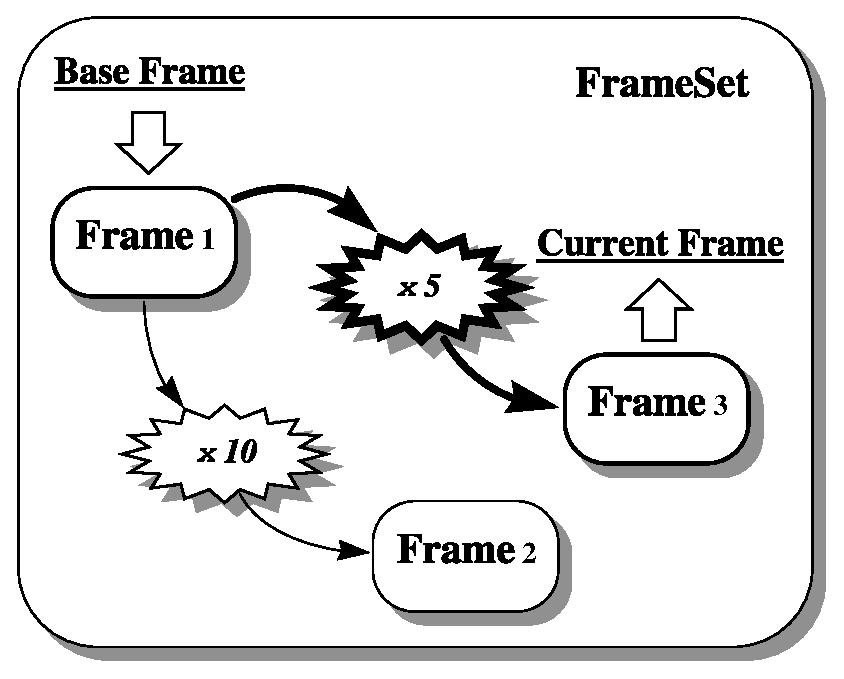
\includegraphics[scale=0.6]{sun210_figures/fsexample.eps}
   \caption{An example FrameSet, in which Frames~2 and 3 are related to
   Frame~1 by multiplying its coordinates by factors of 10 and 5
   respectively. The FrameSet's \htmlref{Base}{Base} attribute has the value 1 and its
   \htmlref{Current}{Current} attribute has the value 3. The transformation performed when
   the FrameSet is used as a Mapping ({\em{i.e.}}\ from its base to
   its current Frame) is shown in bold.}
   \label{fig:fsexample}
   \end{center}
   \end{figure}
   The total number of Frames is given by its read-only \htmlref{Nframe}{Nframe} attribute.
\end{latexonly}
\begin{htmlonly}
   Our example FrameSet now contains three Frames and two Mappings with
   the arrangement shown in the Figure below. The total number of Frames
   is given by its read-only Nframe attribute.
   \begin{quote}
   \begin{figure}
   \label{fig:fsexample}
   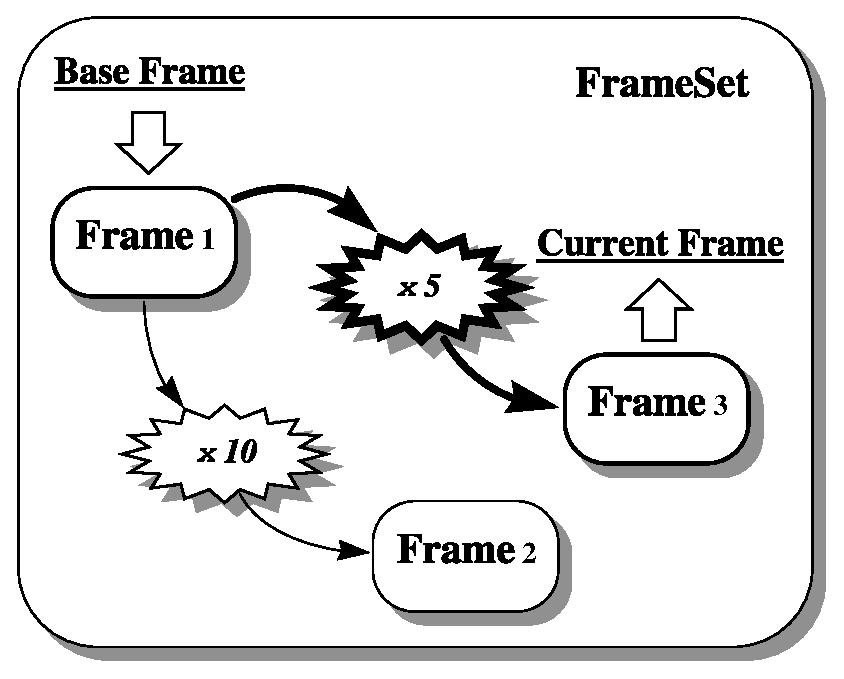
\includegraphics[scale=0.9]{sun210_figures/fsexample.eps}
   \caption{An example FrameSet, in which Frames~2 and 3 are related to
   Frame~1 by multiplying its coordinates by factors of 10 and 5
   respectively. The FrameSet's Base attribute has the value 1 and its
   Current attribute has the value 3. The transformation performed when
   the FrameSet is used as a Mapping ({\em{i.e.}}\ from its base to
   its current Frame) is shown in bold.}
   \end{figure}
   \end{quote}
\end{htmlonly}


\subsection{\label{ss:baseandcurrent}The Base and Current Frames}

At all times, one of the Frames in a \htmlref{FrameSet}{FrameSet} is designated to be its
{\em{base}} \htmlref{Frame}{Frame} and one to be its {\em{current}} Frame
(Figure~\ref{fig:fsexample}). These Frames are identified by two
integer FrameSet attributes, \htmlref{Base}{Base} and \htmlref{Current}{Current}, which hold the indices
of the nominated Frames within the FrameSet.

The existence of the base and current Frames reflects an important
application of FrameSets, which is to attach coordinate systems to
entities such as data arrays, data files, plotting surfaces (for
graphics), {\em{etc.}}  In this context, the base Frame represents the
``native'' coordinate system of the attached entity---for example, the
pixel coordinates of an image or the intrinsic coordinates of a
plotting surface. The other Frames within the FrameSet represent
alternative coordinate systems which may also be used to refer to
positions within that entity.  The current Frame represents the
particular coordinate system which is currently selected for use. For
instance, if an image were being displayed, you would aim to label it
with coordinates corresponding to the current Frame. In order to see a
different coordinate system, a software user would arrange for a
different Frame to be made current.

The choice of base and current Frames may be changed at any time,
simply by assigning new values to the FrameSet's Base and Current
attributes. For example, to make the Frame with index 3 become the
current Frame, you could use:

\small
\begin{verbatim}
      CALL AST_SETI( FRAMESET, 'Current', 3, STATUS )
\end{verbatim}
\normalsize

You can nominate the same Frame to be both the base and current Frame
if you wish.
\label{ss:baseandcurrentdefault}

By default ({\em{i.e.}}\ if the Base or Current attribute is un-set),
the first Frame added to a FrameSet becomes its base Frame and the
last one added becomes its current Frame.\footnote{Although this is
reversed if the FrameSet's \htmlref{Invert}{Invert} attribute is non-zero.} Whenever a
new Frame is added to a FrameSet, the Current attribute is modified so
that the new Frame becomes the current one. This behaviour is
reflected in the state of the example FrameSet in
Figure~\ref{fig:fsexample}.

\subsection{\label{ss:astbaseandastcurrent}Referring to the Base and Current Frames}

It is often necessary to refer to the base and current Frames
(\secref{ss:baseandcurrent}) within a \htmlref{FrameSet}{FrameSet}, but it can be
cumbersome having to obtain their indices from the \htmlref{Base}{Base} and \htmlref{Current}{Current}
attributes on each occasion. To make this easier, two parameter
constants, AST\_\_BASE and AST\_\_CURRENT, are defined in the AST\_PAR
include file and may be used to represent the indices of the base and
current Frames respectively. They may be used whenever a \htmlref{Frame}{Frame} index
is required.

For example, when adding a new Frame to a FrameSet
(\secref{ss:addingframes}), you could use the following to indicate
that the new Frame is related to the existing current Frame, whatever
its index happens to be:

\small
\begin{verbatim}
      INTEGER FRAME, MAPPING

      ...

      CALL AST_ADDFRAME( FRAMESET, AST__CURRENT, MAPPING, FRAME, STATUS )
\end{verbatim}
\normalsize

Of course, the Frame you added would then become the new current
Frame.

\subsection{\label{ss:framesetasmapping}Using a FrameSet as a Mapping}

The \htmlref{FrameSet}{FrameSet} class inherits properties and behaviour from the \htmlref{Frame}{Frame}
class (\secref{ss:frames}) and, in turn, from the \htmlref{Mapping}{Mapping} class
(\secref{ss:mappings}). Its behaviour when used as a Mapping is
particularly important.

Consider, for instance, passing a FrameSet pointer to a coordinate
transformation routine such as \htmlref{AST\_TRAN2}{AST_TRAN2}:

\small
\begin{verbatim}
      INTEGER N
      DOUBLE PRECISION XIN( N ), YIN( N )
      DOUBLE PRECISION XOUT( N ), YOUT( N )

      ...

      CALL AST_TRAN2( FRAMESET, N, XIN, YIN, .TRUE., XOUT, YOUT, STATUS )
\end{verbatim}
\normalsize

The coordinate transformation applied by this FrameSet would be the
one which converts between its base and current Frames. Using the
FrameSet in Figure~\ref{fig:fsexample}, for example, the coordinates
would be multiplied by a factor of 5.  If we instead requested the
FrameSet's inverse transformation, we would be transforming from its
current Frame to its base Frame, so our example FrameSet would then
multiply by a factor of 0.2.

Whenever the choice of base and current Frames changes, the
transformations which a FrameSet performs when used as a Mapping also
change to reflect this. The \htmlref{Nin}{Nin} and \htmlref{Nout}{Nout} attributes may also change in
consequence, because they are determined by the numbers of axes in the
FrameSet's base and current Frames respectively. These numbers need
not necessarily be equal, of course.

Like any Mapping, a FrameSet may also be inverted by changing the
boolean sense of its \htmlref{Invert}{Invert} attribute, {\em{e.g.}}\ using \htmlref{AST\_INVERT}{AST_INVERT}
(\secref{ss:invertingmappings}). If this is happens, the values of the
FrameSet's \htmlref{Base}{Base} and \htmlref{Current}{Current} attributes are interchanged, along with
its Nin and Nout attributes, so that its base and current Frames swap
places. When used as a Mapping, the FrameSet will therefore perform
the inverse transformation to that which it performed previously.

To summarise, a FrameSet may be used exactly like any other Mapping
which inter-relates the coordinate systems described by its base and
current Frames.

\subsection{\label{ss:extractingamapping}Extracting a Mapping from a FrameSet}

Although it is very convenient to use a \htmlref{FrameSet}{FrameSet} when a \htmlref{Mapping}{Mapping} is
required (\secref{ss:framesetasmapping}), a FrameSet necessarily
contains additional information and sometimes this might cause
inefficiency or confusion.  For example, if you wanted to use a
Mapping contained in one FrameSet and insert it into another, it would
probably not be efficient to insert the whole of the first FrameSet
into the second one, although it would work.

In such a situation, the \htmlref{AST\_GETMAPPING}{AST_GETMAPPING} function allows you to
extract a Mapping from a FrameSet. You do this by specifying the two
Frames which the Mapping should inter-relate using their indices
within the FrameSet. For example:

\small
\begin{verbatim}
      MAP = AST_GETMAPPING( FRAMESET, 2, 3, STATUS )
\end{verbatim}
\normalsize

would return a pointer to a Mapping that converted between Frames~2
and 3 in the FrameSet. Its inverse transformation would then convert
in the opposite direction, {\em{i.e.}}\ between Frames~3 and 2.  Note
that this Mapping might not be independent of the Mappings contained
within the FrameSet---{\em{i.e.}}\ they may share sub-Objects---so
\htmlref{AST\_COPY}{AST_COPY} should be used to make a copy if you need to guarantee
independence (\secref{ss:copyingobjects}).

Very often, the Mapping returned by AST\_GETMAPPING will be a compound
Mapping, or \htmlref{CmpMap}{CmpMap} (\secref{ss:cmpmaps}). This reflects the fact that
conversion between the two Frames may need to be done {\em{via}} an
intermediate coordinate system so that several stages may be involved.
You can, however, easily simplify this Mapping (where this is possible)
by using the \htmlref{AST\_SIMPLIFY}{AST_SIMPLIFY} function (\secref{ss:simplifyingcmpmaps})
and this is recommended if you plan to use it for transforming a large
amount of data.

\subsection{\label{ss:framesetasframe}Using a FrameSet as a Frame}

A \htmlref{FrameSet}{FrameSet} can also be used as a \htmlref{Frame}{Frame}, in which capacity it almost
always behaves as if its current Frame had been used instead. For
example, if you request the \htmlref{Title}{Title} attribute of a FrameSet using:

\small
\begin{verbatim}
      CHARACTER * ( 80 ) TITLE

      ...

      TITLE = AST_GETC( FRAMESET, 'Title', STATUS )
\end{verbatim}
\normalsize

the result will be the Title of the current Frame, or a suitable
default if the current Frame's Title attribute is un-set. The same
also applies to other attribute operations---{\em{i.e.}}\ setting,
clearing and testing attributes.  Most attributes shared by both
Frames and FrameSets behave in this way, such as \htmlref{Naxes}{Naxes}, \htmlref{Label(axis)}{Labelaxis},
\htmlref{Format(axis)}{Formataxis}, {\em{etc.}} There are, however, a few exceptions:

\begin{quote}
\begin{description}
\item[\htmlref{Class}{Class}]\mbox{}\\
Has the value ``FrameSet''.

\item[\htmlref{ID}{ID}]\mbox{}\\
Identifies the particular FrameSet (not its current Frame).

\item[\htmlref{Nin}{Nin}]\mbox{}\\
Equals the number of axes in the FrameSet's base Frame.

\item[\htmlref{Invert}{Invert}]\mbox{}\\
Is independent of any of the Objects within the FrameSet.

\item[\htmlref{Nobject}{Nobject}]\mbox{}\\
Counts the number of active FrameSets.

\item[\htmlref{RefCount}{RefCount}]\mbox{}\\
Counts the number of active pointers to the FrameSet (not to its
current Frame).
\end{description}
\end{quote}

Note that the set of attributes possessed by a FrameSet can vary,
depending on the nature of its current Frame. For example, if the
current Frame is a \htmlref{SkyFrame}{SkyFrame} (\secref{ss:skyframes}), then the FrameSet
will acquire an \htmlref{Equinox}{Equinox} attribute from it which can be set, enquired,
{\em{etc.}}  However, if the current Frame is changed to be a basic
Frame, which does not have an Equinox attribute, then this attribute
will be absent from the FrameSet as well. Any attempt to reference it
will then result in an error.

\subsection{Extracting a Frame from a FrameSet}

Although a \htmlref{FrameSet}{FrameSet} may be used in place of its current \htmlref{Frame}{Frame} in most
situations, it is sometimes convenient to have direct access to a
specified Frame within it. This may be obtained using the
\htmlref{AST\_GETFRAME}{AST_GETFRAME} function, as follows:

\small
\begin{verbatim}
      FRAME = AST_GETFRAME( FRAMESET, AST__BASE, STATUS )
\end{verbatim}
\normalsize

This would return a pointer (not a copy) to the base Frame within the
FrameSet. Note the use of AST\_\_BASE
(\secref{ss:astbaseandastcurrent}) as shorthand for the value of the
FrameSet's \htmlref{Base}{Base} attribute, which gives the base Frame's index.

\subsection{Removing a Frame from a FrameSet}

Removing a \htmlref{Frame}{Frame} from a \htmlref{FrameSet}{FrameSet} is straightforward and is performed
using the \htmlref{AST\_REMOVEFRAME}{AST_REMOVEFRAME} routine. You identify the Frame you wish to
remove in the usual way, by giving its index within the FrameSet. For
example, the following would remove the Frame with index 1:

\small
\begin{verbatim}
      CALL AST_REMOVEFRAME( FRAMESET, 1, STATUS );
\end{verbatim}
\normalsize

The only restriction is that you cannot remove the last remaining
Frame because a FrameSet must always contain at least one Frame.  When
a Frame is removed, the Frames which follow it are re-numbered
({\em{i.e.}}\ their indices are reduced by one) so as to preserve the
sequence of consecutive Frame indices.  The FrameSet's \htmlref{Nframe}{Nframe}
attribute is also decremented.

If appropriate, AST\_REMOVEFRAME will modify the FrameSet's \htmlref{Base}{Base}
and/or \htmlref{Current}{Current} attributes so that they continue to identify the same
Frames as previously. If either the base or current Frame is removed,
however, the corresponding attribute will become un-set, so that it
reverts to its default value (\secref{ss:baseandcurrentdefault}) and
therefore identifies an alternative Frame.

Note that it is quite permissible to remove any Frame from a FrameSet,
even although other Frames may appear to depend on it. For example, in
Figure~\ref{fig:fsexample}, if Frame~1 were removed, the correct
relationship between Frames~2 and 3 would still be preserved, although
they would be re-numbered as Frames~1 and 2.

\cleardoublepage
\section{\label{ss:fshigher}Higher Level Operations on FrameSets}

\subsection{\label{ss:framesetsfromconvert}Creating FrameSets with AST\_CONVERT}

Before considering the important subject of using FrameSets to convert
between coordinate systems (\secref{ss:framesetconverting}), let us
return briefly to reconsider the output generated by \htmlref{AST\_CONVERT}{AST_CONVERT}. We
used this function earlier (\secref{ss:introducingconversion}), when
converting between the coordinate systems represented by various kinds
of \htmlref{Frame}{Frame}, and indicated that it returns a \htmlref{FrameSet}{FrameSet} to represent the
coordinate conversion it identifies. We are now in a position to
examine the structure of this FrameSet.

Take our earlier example (\secref{ss:convertingskyframes}) of
converting between the celestial coordinate systems represented by two
SkyFrames:

\small
\begin{verbatim}
      INCLUDE 'AST_PAR'
      INTEGER SKYFRAME1, SKYFRAME2, STATUS

      STATUS = 0

      ...

      SKYFRAME1 = AST_SKYFRAME( 'System=FK4-NO-E, Epoch=B1958, Equinox=B1960', STATUS )
      SKYFRAME2 = AST_SKYFRAME( 'System=Ecliptic, Equinox=J2010.5', STATUS )

      CVT = AST_CONVERT( SKYFRAME1, SKYFRAME2, ' ', STATUS )
\end{verbatim}
\normalsize

\begin{latexonly}
   This will produce a pointer, CVT, to the FrameSet shown in
   Figure~\ref{fig:fsconvert}.
   \begin{figure}[bhtp]
   \begin{center}
   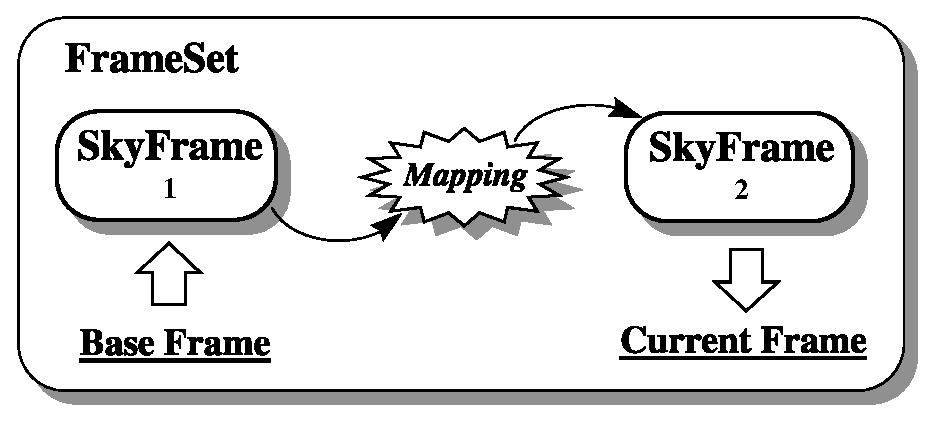
\includegraphics[scale=0.65]{sun210_figures/fsconvert.eps}
   \caption{The FrameSet produced when AST\_CONVERT is used to convert
   between the coordinate systems represented by two SkyFrames. The
   source \htmlref{SkyFrame}{SkyFrame} becomes the base Frame, while the destination SkyFrame
   becomes the current Frame. The \htmlref{Mapping}{Mapping} between them implements the
   required conversion.}
   \label{fig:fsconvert}
   \end{center}
   \end{figure}
\end{latexonly}
\begin{htmlonly}
   This will produce a pointer, CVT, to the FrameSet shown in the Figure
   below.
   \begin{quote}
   \begin{figure}[bhtp]
   \label{fig:fsconvert}
   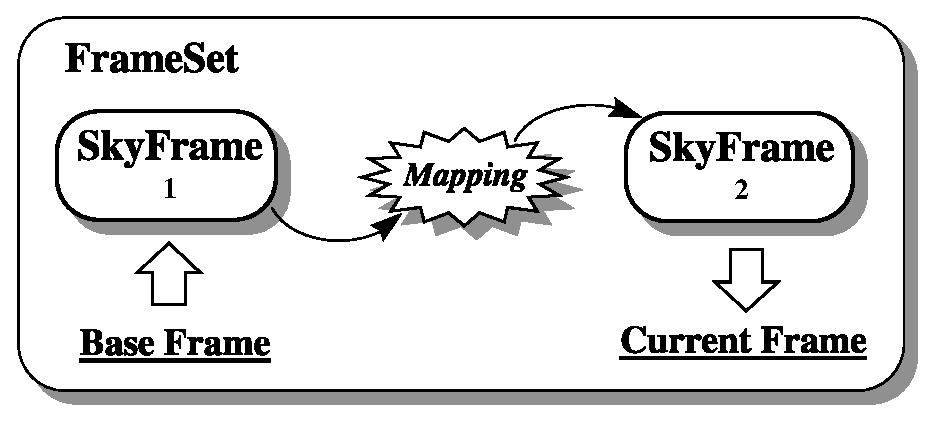
\includegraphics[scale=1.0]{sun210_figures/fsconvert.eps}
   \caption{The FrameSet produced when AST\_CONVERT is used to convert
   between the coordinate systems represented by two SkyFrames. The
   source SkyFrame becomes the base Frame, while the destination SkyFrame
   becomes the current Frame. The Mapping between them implements the
   required conversion.}
   \end{figure}
   \end{quote}
\end{htmlonly}
As can be seen, this FrameSet contains just two Frames.  The source
Frame supplied to AST\_CONVERT becomes its base Frame, while the
destination Frame becomes its current Frame. (The FrameSet, of course,
simply holds pointers to these Frames, rather than making copies.) The
Mapping which relates the base Frame to the current Frame is the one
which implements the required conversion.

As we noted earlier (\secref{ss:convertingskyframes}), the FrameSet
returned by AST\_CONVERT may be used both as a Mapping and as a Frame
to perform most of the functions you are likely to need. However, the
Mapping may be extracted for use on its own if necessary, using
\htmlref{AST\_GETMAPPING}{AST_GETMAPPING} (\secref{ss:extractingamapping}), for example:

\small
\begin{verbatim}
      INTEGER MAPPING

      ...

      MAPPING = AST_GETMAPPING( CVT, AST__BASE, AST__CURRENT, STATUS )
\end{verbatim}
\normalsize

\subsection{\label{ss:framesetconverting}Converting between FrameSet Coordinate Systems}

\begin{latexonly}
   We now consider the process of converting between the coordinate
   systems represented by two FrameSets. This is a most important
   operation, as a subsequent example (\secref{ss:registeringimages})
   will show, and is illustrated in Figure~\ref{fig:fsalign}.
   \begin{figure}
   \begin{center}
   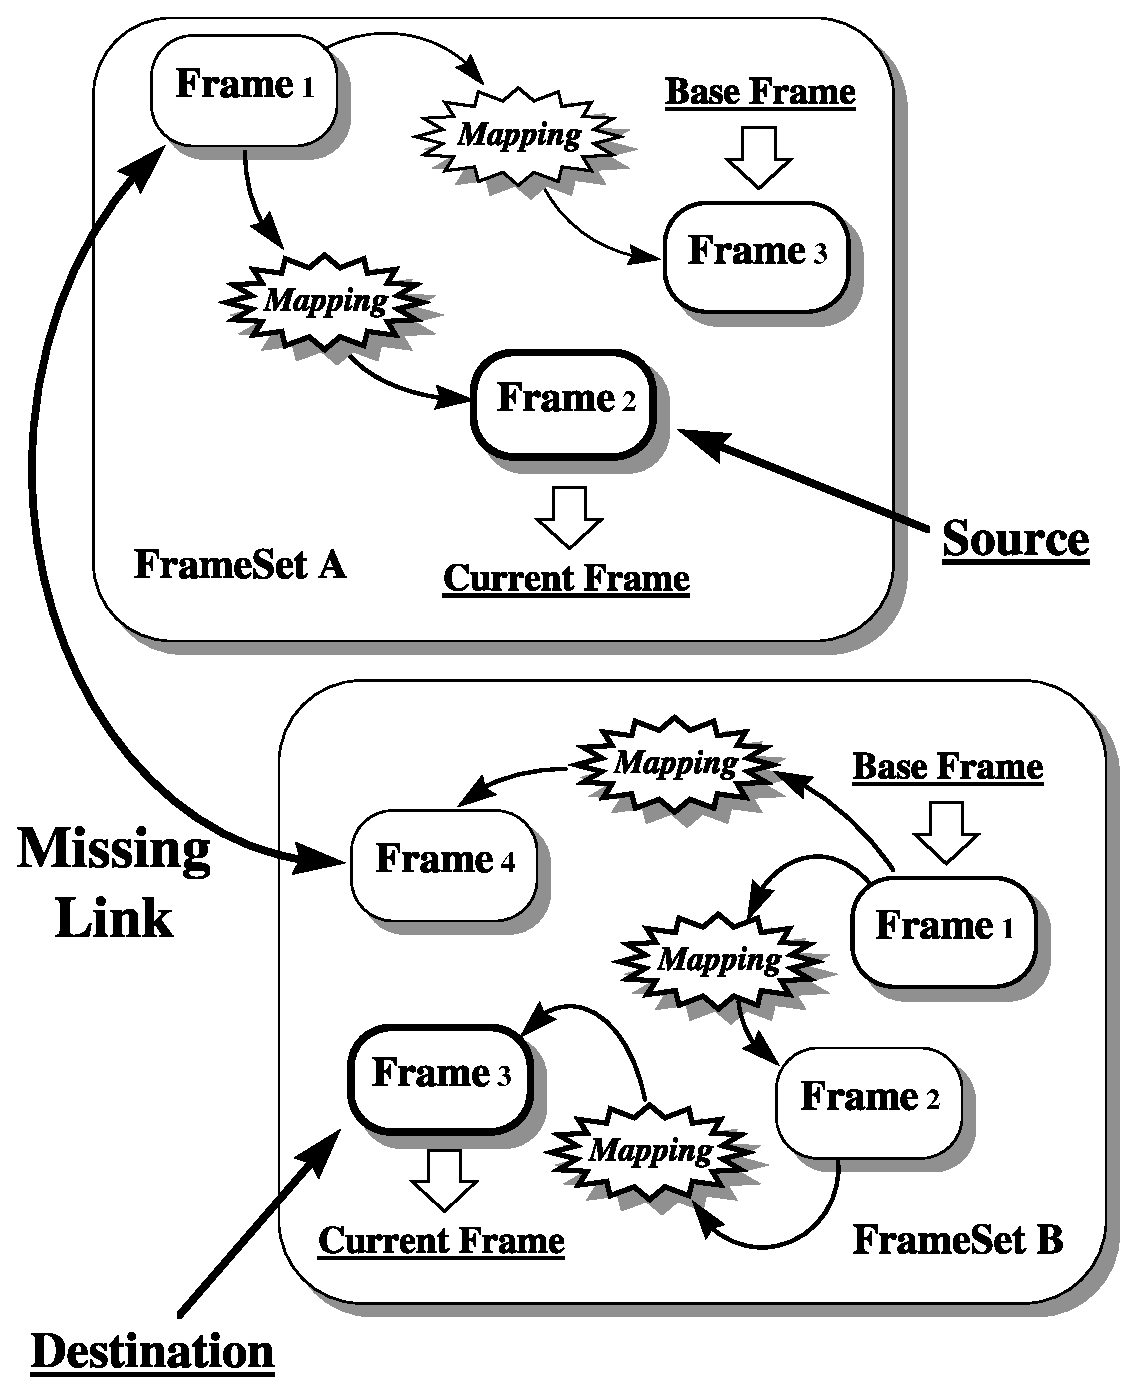
\includegraphics[scale=0.6]{sun210_figures/fsalign.eps}
   \caption{Conversion between two FrameSets is performed by establishing
   a link between a pair of Frames, one from each \htmlref{FrameSet}{FrameSet}. If conversion
   between these two Frames is possible, then a route for converting
   between the current Frames of both FrameSets can also be found. In
   practice, there may be many ways of pairing Frames to find the
   ``missing link'', so the Frames' \htmlref{Domain}{Domain} attribute may be used to
   narrow the choice.}
   \label{fig:fsalign}
   \end{center}
   \end{figure}
\end{latexonly}
\begin{htmlonly}
   We now consider the process of converting between the coordinate
   systems represented by two FrameSets. This is a most important
   operation, as a subsequent example (\secref{ss:registeringimages})
   will show, and is illustrated in the Figure below.
   \begin{quote}
   \begin{figure}
   \label{fig:fsconvert}
   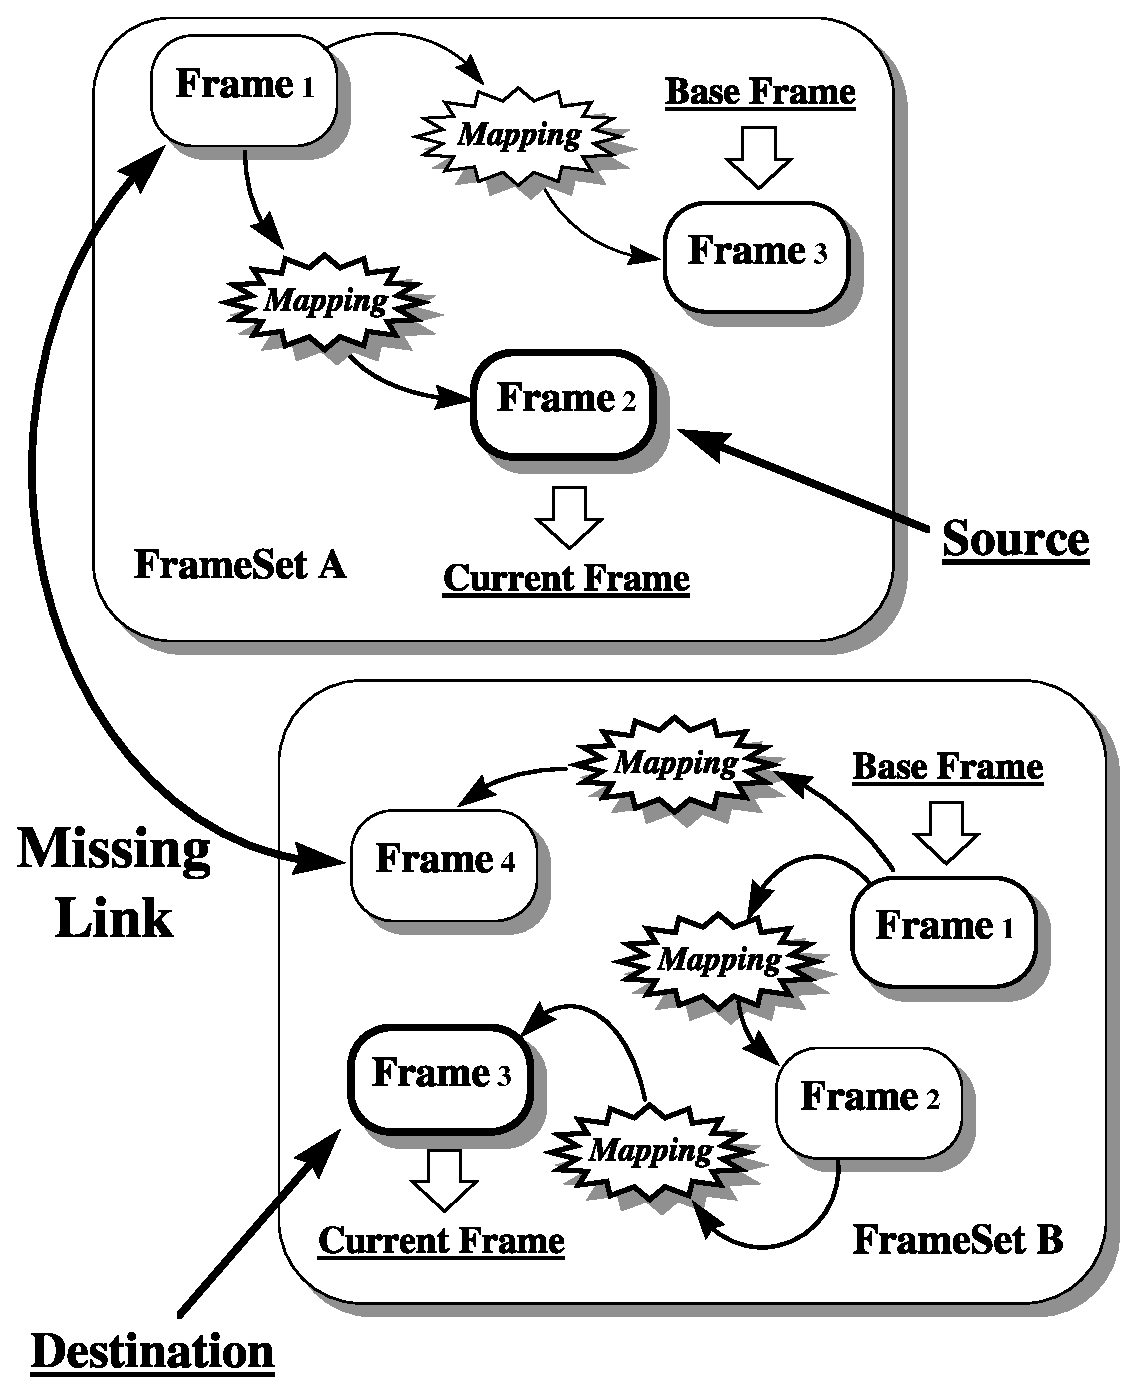
\includegraphics[scale=1.0]{sun210_figures/fsalign.eps}
   \caption{Conversion between two FrameSets is performed by establishing
   a link between a pair of Frames, one from each FrameSet. If conversion
   between these two Frames is possible, then a route for converting
   between the current Frames of both FrameSets can also be found. In
   practice, there may be many ways of pairing Frames to find the
   ``missing link'', so the Frames' Domain attribute may be used to
   narrow the choice.}
   \end{figure}
   \end{quote}
\end{htmlonly}
Recalling (\secref{ss:framesetasframe}) that a FrameSet will behave
like its current \htmlref{Frame}{Frame} when necessary, conversion between two
FrameSets is performed using \htmlref{AST\_CONVERT}{AST_CONVERT}
(\secref{ss:convertingskyframes}), but supplying pointers to FrameSets
instead of Frames. The effect of this is to convert between the
coordinate systems represented by the current Frames of each FrameSet:

\small
\begin{verbatim}
      INTEGER FRAMESETA, FRAMESETB

      ...

      CVT = AST_CONVERT( FRAMESETA, FRAMESETB, 'SKY', STATUS )
\end{verbatim}
\normalsize

When using FrameSets, we are presented with considerably more
conversion options than when using Frames alone. This is because each
current Frame is related to all the other Frames in its respective
FrameSet. Therefore, if we can establish a link between any pair of
Frames, one from each FrameSet, we can form a complete conversion path
between the two current Frames (Figure~\ref{fig:fsalign}).

This expanded range of options is, of course, precisely the
intention. By connecting Frames together within a FrameSet, we have
extended the range of coordinate systems that can be reached from any
one of them.  We are therefore no longer restricted to converting
between Frames with the same Domain value (\secref{ss:framedomains}),
but can go {\em{via}} a range of intermediate coordinate systems in
order to make the connection we require. Transformation between
different domains has therefore become possible because, in assembling
the FrameSets, we provided the additional information needed to
inter-relate them.

It is important to appreciate, however, that the choice of ``missing
link'' is crucial in determining the conversion that results.
Although each FrameSet may be perfectly self-consistent internally,
this does not mean that all conversion paths through the combined
network of Mappings are equivalent. Quite the contrary in fact:
everything depends on where the inter-connecting link between the two
FrameSets is made.  In practice, there may be a large number of
possible pairings of Frames and hence of possible links. Other factors
must therefore be used to restrict the choice. These are:

\begin{enumerate}
\item Not every possible pairing of Frames is legitimate. For example,
you cannot convert directly between a basic Frame and a \htmlref{SkyFrame}{SkyFrame} which
belong to different classes, so such pairings will be ignored.

\item In a similar way, you cannot convert directly between Frames
with different Domain values (\secref{ss:framedomains}). If the Domain
attribute is used consistently (typically only one Frame in each
FrameSet will have a particular Domain value), then this further
restricts the choice.

\item The third argument of AST\_CONVERT may then be used to specify
explicitly which Domain value the paired Frames should have. You may
also supply a comma-separated list of preferences here (see below).

\item If the above steps fail to uniquely identify the link, then the
first suitable pairing of Frames is used, so that any ambiguity is
resolved by the order in which Frames are considered for pairing (see
the description of the AST\_CONVERT function in
\appref{ss:functiondescriptions} for details of the search
order).\footnote{If you find that how this ambiguity is resolved
actually makes a difference to the conversion that results, then you
have probably constructed a FrameSet which lacks internal
self-consistency. For example, you might have two Frames representing
indistinguishable coordinate systems but inter-related by a non-null
\htmlref{Mapping}{Mapping}.}
\end{enumerate}

In the example above we supplied the string ``SKY'' as the third
argument of AST\_CONVERT. This constitutes a request that a pair of
Frames with
the Domain value SKY ({\em{i.e.}}\ representing celestial coordinate
systems) should be used to inter-relate the two FrameSets. Note that
this does not specify which celestial coordinate system to use, but is
a general request that the two FrameSets be inter-related using
coordinates on the celestial sphere.

Of course, it may be that this request cannot be met because there may
not be a celestial coordinate system in both FrameSets. If this is
likely to happen, we can supply a list of preferences, or a
{\em{domain search path,}}
as the third argument to AST\_CONVERT, such as
the following:

\small
\begin{verbatim}
      CVT = AST_CONVERT( FRAMESETA, FRAMESETB, 'SKY,PIXEL,GRID,', STATUS )
\end{verbatim}
\normalsize

Now, if the two FrameSets cannot be inter-related using the SKY domain,
AST\_CONVERT will attempt to use the PIXEL domain instead. If this
also fails, it will try the GRID domain. A blank field in the domain
search path (here indicated by the final comma) allows any Domain
value to be used. This can be employed as a last resort when all else
has failed.

If astConvert succeeds in identifying a conversion, it will return a
pointer to a FrameSet (\secref{ss:framesetsfromconvert}) in which the
source and destination Frames are inter-connected by the required
Mapping. In this case, of course, these Frames will be the current
Frames of the two FrameSets, but in all other respects the returned
FrameSet is the same as when converting between Frames.

Very importantly, however, AST\_CONVERT may modify the FrameSets you
are converting between. It does this, in order to indicate which
pairing of Frames was used to inter-relate them, by changing the \htmlref{Base}{Base}
attribute for each FrameSet so that the Frame used in the pairing
becomes its base Frame (\secref{ss:baseandcurrent}).

Finally, note that AST\_CONVERT may also be used to convert between a
FrameSet and a Frame, or {\em{vice versa.}} If a pointer to a Frame is
supplied for either the first or second argument, it will behave like
a FrameSet containing only a single Frame.

\subsection{\label{ss:registeringimages}Example---Registering Two Images}

Consider two images which have been calibrated by attaching FrameSets
to them, such that the base \htmlref{Frame}{Frame} of each \htmlref{FrameSet}{FrameSet} corresponds to the
raw data grid coordinates of each image (the GRID domain of
\secref{ss:domainconventions}). Suppose, also, that these FrameSets
contain an unknown number of other Frames, representing alternative
world coordinate systems.  What we wish to do is register these two
images, such that we can transform from a position in the data grid of
one into the corresponding position in the data grid of the other.
This is a very practical example because images will typically be
calibrated using FrameSets in precisely this way.

The first step will probably involve making a copy of both FrameSets
(using \htmlref{AST\_COPY}{AST_COPY}---\secref{ss:copyingobjects}), since we will be
modifying them. Let ``frameseta'' and ``framesetb'' be pointers to
these copies. Since we want to convert between the base Frames of
these FrameSets ({\em{i.e.}}\ their data grid coordinates), the next
step is to make these Frames current. This is simply done by inverting
both FrameSets, which interchanges their base and current
Frames. astInvert will perform this task:

\small
\begin{verbatim}
      CALL AST_INVERT( FRAMESETA, STATUS )
      CALL AST_INVERT( FRAMESETB, STATUS )
\end{verbatim}
\normalsize

To identify the required conversion, we now use \htmlref{AST\_CONVERT}{AST_CONVERT},
supplying a suitable domain search path with which we would like our
two images to be registered:

\small
\begin{verbatim}
      CVT = AST_CONVERT( FRAMESETA, FRAMESETB, 'SKY,PIXEL,GRID', STATUS )
      IF ( CVT .EQ. AST__NULL ) THEN
         <no conversion was possible>
      ELSE
         <conversion was possible>
      END IF
\end{verbatim}
\normalsize

The effects of this are:

\begin{enumerate}
\item AST\_CONVERT first attempts to register the two images on the
celestial sphere ({\em{i.e.}}\ using the SKY domain). To do this, it
searches for a celestial coordinate system, although not necessarily
the same one, attached to each image.  If it finds a suitable pair of
coordinate systems, it then registers the images by matching
corresponding positions on the sky.

\item If this fails, AST\_CONVERT next tries to match positions in the
PIXEL domain (\secref{ss:framedomains}). If it succeeds, the two
images will then be registered so that their corresponding pixel
positions correspond. If the PIXEL domain is offset from the data grid
(as typically happens in data reduction systems which implement a
``pixel origin''), then this will be correctly accounted for.

\item If this also fails, the GRID domain is finally used. This will
result in image registration by matching corresponding points in the
data grids used by both images. This means they will be
aligned so that the first element their data arrays correspond.

\item If all of the above fail, AST\_CONVERT will return the value
AST\_\_NULL. Otherwise a pointer to a FrameSet will be returned.
\end{enumerate}

The resulting CVT FrameSet may then be used directly
(\secref{ss:convertingskyframes}) to convert between positions in the
data grid of the first image and corresponding positions in the data
grid of the second image.

To determine which domain was used to achieve registration,
we can use the fact that the \htmlref{Base}{Base} attribute of each FrameSet is set by
AST\_CONVERT to indicate which intermediate Frames were used. We
can therefore simply invert either FrameSet (to make its base Frame
become the current one) and then enquire the \htmlref{Domain}{Domain} value:

\small
\begin{verbatim}
      CHARACTER * ( 20 ) DOMAIN

      ...


      CALL AST_INVERT( FRAMESETA, STATUS )
      DOMAIN = AST_GETC( FRAMESETA, 'Domain', STATUS )
\end{verbatim}
\normalsize

If conversion was successful, the result will be one of the strings
``SKY'', ``PIXEL'' or ``GRID''.

\subsection{\label{ss:remapframe}Re-Defining a FrameSet Coordinate System}

As discussed earlier (\secref{ss:baseandcurrent}), an important
application of a \htmlref{FrameSet}{FrameSet} is to allow coordinate system information to
be attached to entities such as images in order to calibrate them. In
addition, one of the main objectives of AST is to simplify the
propagation of such information through successive stages of data
processing, so that it remains consistent with the associated image
data.

In such a situation, the FrameSet's base \htmlref{Frame}{Frame} would correspond with
the image's data grid coordinates and its other Frames (if any) with
the various alternative world coordinate systems associated with the
image.  If the data processing being performed does not change the
relationship between the image's data grid coordinates and any of the
associated world coordinate systems, then propagation of the WCS
information is straightforward and simply involves copying the
FrameSet associated with the image.

If any of these relationships change, however, then corresponding
changes must be made to the way Frames within the FrameSet are
inter-related. By far the most common case occurs when the image
undergoes some geometrical transformation resulting in ``re-gridding''
on to another data grid, but the same principles can be applied to any
re-definition of a coordinate system.

To pursue the re-gridding example, we would need to modify our
FrameSet to account for the fact that the image's data grid coordinate
system (corresponding to the FrameSet's base Frame) has
changed. Looking at the steps needed in detail, we might proceed as
follows:

\begin{enumerate}
\item Create a \htmlref{Mapping}{Mapping} which represents the relationship between the
original data grid coordinate system and the new one.

\item Obtain a Frame to represent the new data grid coordinate system
(we could re-use the original base Frame here, using \htmlref{AST\_GETFRAME}{AST_GETFRAME} to
obtain a pointer to it).

\item Add the new Frame to the FrameSet, related to the original base
Frame by the new Mapping. This Frame now represents the new data grid
coordinate system and is correctly related to all the other Frames
present.\footnote{This is because any transformation to or from this
new Frame must go {\em{via}} the base Frame representing the original
data grid coordinate system, which we assume was correctly related to
all the other Frames present.}

\item Remove the original base Frame (representing the old data grid
coordinate system).

\item Make the new Frame the base Frame and restore the original
current Frame.
\end{enumerate}

\begin{latexonly}
   The effect of these steps is to change the relationship between the
   base Frame and all the other Frames present. It is as if a new Mapping
   has been interposed between the Frame we want to alter and all the
   other Frames within the FrameSet (Figure~\ref{fig:fsremap}).
   \begin{figure}[hbtp]
   \begin{center}
   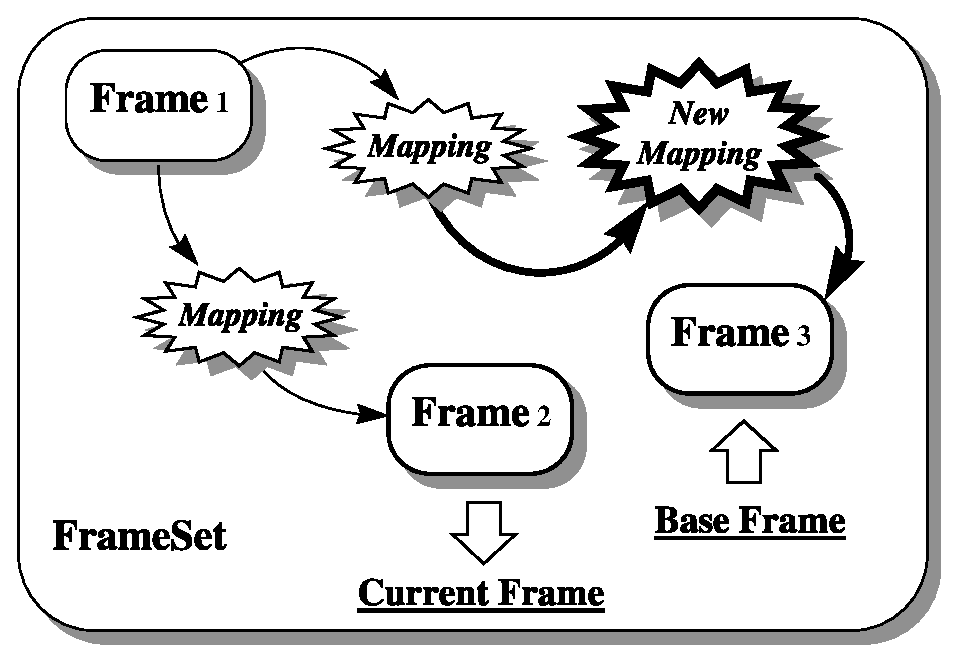
\includegraphics[scale=0.6]{sun210_figures/fsremap.eps}
   \caption{The effect of \htmlref{AST\_REMAPFRAME}{AST_REMAPFRAME} is to interpose a Mapping between
   a nominated Frame within a FrameSet and the remaining contents of the
   FrameSet. This effectively ``re-defines'' the coordinate system
   represented by the affected Frame. It may be used to compensate (say)
   for geometrical changes made to an associated image. The
   inter-relationships between all the other Frames within the FrameSet
   remain unchanged.}
   \label{fig:fsremap}
   \end{center}
   \end{figure}
\end{latexonly}
\begin{htmlonly}
   The effect of these steps is to change the relationship between the
   base Frame and all the other Frames present. It is as if a new Mapping
   has been interposed between the Frame we want to alter and all the
   other Frames within the FrameSet (see Figure below).
   \begin{quote}
   \begin{figure}[hbtp]
   \label{fig:fsremap}
   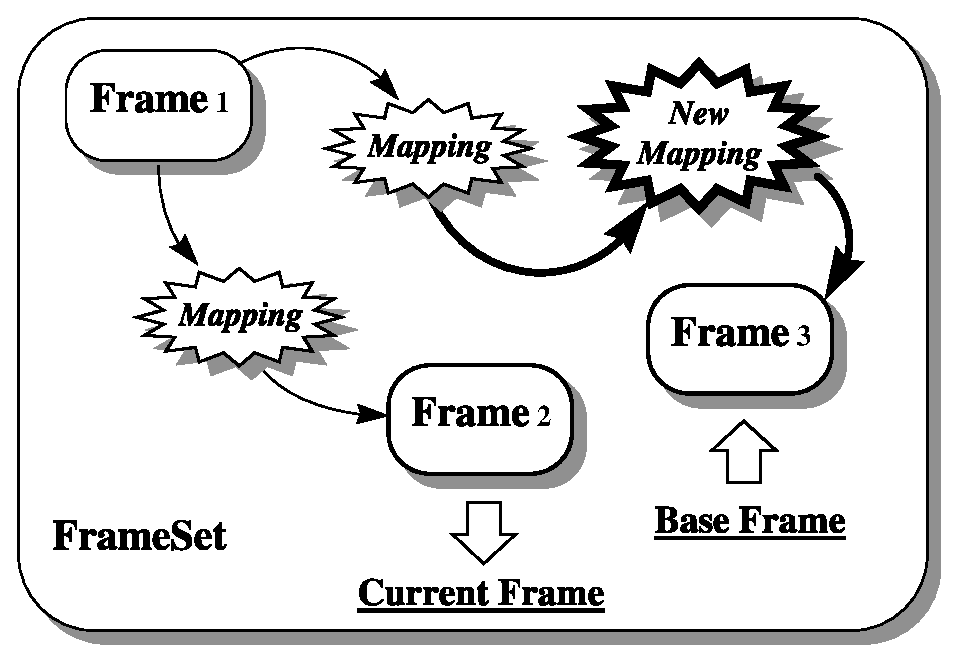
\includegraphics[scale=0.9]{sun210_figures/fsremap.eps}
   \caption{The effect of AST\_REMAPFRAME is to interpose a Mapping between
   a nominated Frame within a FrameSet and the remaining contents of the
   FrameSet. This effectively ``re-defines'' the coordinate system
   represented by the affected Frame. It may be used to compensate (say)
   for geometrical changes made to an associated image. The
   inter-relationships between all the other Frames within the FrameSet
   remain unchanged.}
   \end{figure}
   \end{quote}
\end{htmlonly}

Performing the steps above is rather lengthy, however, so the
AST\_REMAPFRAME function is provided to perform all of these
operations in one go.  A practical example of its use is given below
(\secref{ss:wcsprocessingexample}).

\subsection{\label{ss:wcsprocessingexample}Example---Binning an Image}

As an example of using \htmlref{AST\_REMAPFRAME}{AST_REMAPFRAME}, consider a case where the
pixels of a 2-dimensional image have been binned 2$\times$2, so as to
reduce the image size by a factor of two in each dimension.  We must
now modify the associated \htmlref{FrameSet}{FrameSet} to reflect this change to the
image. Much the same process would be needed for any other geometrical
change the image might undergo.

We first set up a \htmlref{Mapping}{Mapping} (a \htmlref{WinMap}{WinMap} in this case) which relates the
data grid coordinates in the original image to those in the new one:

\small
\begin{verbatim}
      INTEGER WINMAP
      DOUBLE PRECISION INA( 2 ), INB( 2 ), OUTA( 2 ), OUTB( 2 )
      DATA INA / 0.5D0, 0.5D0 /
      DATA INB / 2.5D0, 2.5D0 /
      DATA OUTA / 0.5D0, 0.5D0 /
      DATA OUTB / 1.5DO, 1.5DO /

      ...

      WINMAP = AST_WINMAP( 2, INA, INB, OUTA, OUTB, ' ', STATUS )
\end{verbatim}
\normalsize

Here, we have simply set up arrays containing the data grid
coordinates of the bottom left and top right corners of the first
element in the output image (OUTA and OUTB) and the corresponding
coordinates in the input image (INA and INB). \htmlref{AST\_WINMAP}{AST_WINMAP} then creates
a WinMap which performs the required transformation. We do not need to
know the size of the image.

We can then pass this WinMap to AST\_REMAPFRAME. This modifies the
relationship between our FrameSet's base \htmlref{Frame}{Frame} and the other Frames in
the FrameSet, so that the base Frame represents the data grid
coordinate system of the new image rather than the old one:

\small
\begin{verbatim}
      INTEGER FRAMESET

      ...

      CALL AST_REMAPFRAME( FRAMESET, AST__BASE, WINMAP, STATUS )
\end{verbatim}
\normalsize

Any other coordinate systems described by the FrameSet, no matter how
many of these there might be, are now correctly associated with the
new image.

\subsection{\label{ss:framesetintegrity}Maintaining the Integrity of FrameSets}

When constructing a \htmlref{FrameSet}{FrameSet}, you are provided with a framework into
which you can place any combination of Frames and Mappings that you
wish. There are relatively few constraints on this process and no
checks are performed to see whether the FrameSet you construct makes
physical sense.  It is quite possible, for example, to construct a
FrameSet containing two identical SkyFrames which are inter-related by
a non-unit \htmlref{Mapping}{Mapping}. AST will not object if you do this, but it makes
no sense, because applying a non-unit Mapping to any set of celestial
coordinates cannot yield positions that are still in the original
coordinate system.  If you use such a FrameSet to perform coordinate
conversions, you are likely to get unpredictable results because the
information in the FrameSet is corrupt.

It is, of course, your responsibility as a programmer to ensure the
validity of any information which you insert into a
FrameSet. Normally, this is straightforward and simply consists of
formulating your problem correctly (a diagram can often help to
clarify how coordinate systems are inter-related) and writing the
appropriate bug-free code to construct the FrameSet. However, once you
start to modify an existing FrameSet, there are new opportunities for
corrupting it!

Consider, for example, a FrameSet whose current \htmlref{Frame}{Frame} is a
\htmlref{SkyFrame}{SkyFrame}. We can set a new value for this SkyFrame's \htmlref{Equinox}{Equinox} attribute
simply by using \htmlref{AST\_SET}{AST_SET} on the FrameSet, as follows:

\small
\begin{verbatim}
      CALL AST_SET( FRAMESET, 'Equinox=J2010', STATUS )
\end{verbatim}
\normalsize

The effect of this will be to change the celestial coordinate system
which the current Frame represents. You can see, however, that this
has the potential to make the FrameSet corrupt unless corresponding
changes are also made to the Mapping which relates this SkyFrame to
the other Frames within the FrameSet. In fact, it is a general rule
that any change to a FrameSet which affects its current Frame can
potentially require corresponding changes to the FrameSet's Mappings
in order to maintain its overall integrity.

Fortunately, once you have stored valid information in a FrameSet, AST
will look after these details for you automatically, so that the
FrameSet's integrity is maintained. In the example above, it would do
this by appropriately re-mapping the current Frame (as if
\htmlref{AST\_REMAPFRAME}{AST_REMAPFRAME} had been used---\secref{ss:remapframe}) in response to
the use of AST\_SET. One way of illustrating this process is as
follows:

\small
\begin{verbatim}
      INTEGER SKYFRAME

      ...

      SKYFRAME = AST_SKYFRAME( ' ', STATUS )
      FRAMESET = AST_FRAMESET( SKYFRAME, STATUS )
      CALL AST_ADDFRAME( FRAMESET, 1, AST_UNITMAP( 2, ' ', STATUS )
     :                   SKYFRAME, STATUS )
\end{verbatim}
\normalsize

This constructs a trivial FrameSet whose base and current Frames are
both the same SkyFrame connected by a \htmlref{UnitMap}{UnitMap}. You can think of this
as a ``pipe'' connecting two coordinate systems. At present, these two
systems represent identical ICRS coordinates, so the FrameSet
implements a unit Mapping. We can change the coordinate system on the
current end of this pipe as follows:

\small
\begin{verbatim}
      CALL AST_SET( FRAMESET, 'System=Ecliptic, Equinox=J2010', STATUS )
\end{verbatim}
\normalsize

and the Mapping which the FrameSet implements would change
accordingly. To change the coordinate system on the base end of the
pipe, we might use:

\small
\begin{verbatim}
      CALL AST_INVERT( FRAMESET )
      CALL AST_SET( FRAMESET, 'System=Galactic', STATUS )
      CALL AST_INVERT( FRAMESET )
\end{verbatim}
\normalsize

The FrameSet would then convert between galactic and ecliptic
coordinates.

Note that AST\_SET is not the only function which has this effect:
\htmlref{AST\_CLEAR}{AST_CLEAR} behaves similarly, as also does \htmlref{AST\_PERMAXES}{AST_PERMAXES}
(\secref{ss:permutingaxes}). If you need to circumvent this mechanism
for any reason, this can be done by going behind the scenes and
obtaining a pointer directly to the Frame you wish to modify. Consider
the following, for example:

\small
\begin{verbatim}
      SKYFRAME = AST_GETFRAME( FRAMESET, AST__CURRENT, STATUS )
      CALL AST_SET( SKYFRAME, 'Equinox=J2010', STATUS )
      CALL AST_ANNUL( SKYFRAME, STATUS )
\end{verbatim}
\normalsize

Here, AST\_SET is applied to the SkyFrame pointer rather than the
FrameSet pointer, so the usual checks on FrameSet integrity do not
occur. The SkyFrame's Equinox attribute will therefore be modified
without any corresponding change to the FrameSet's Mappings.  In this
case you must take responsibility yourself for maintaining the
FrameSet's integrity, perhaps through appropriate use of
AST\_REMAPFRAME.

\subsection{Merging FrameSets}

\begin{latexonly}
   As well as adding individual Frames to a \htmlref{FrameSet}{FrameSet}
   (\secref{ss:addingframes}), it is also possible to add complete sets of
   inter-related Frames which are contained within another
   FrameSet. This, of course, corresponds to the process of merging two
   FrameSets (Figure~\ref{fig:fsmerge}).
   \begin{figure}[hbtp]
   \begin{center}
   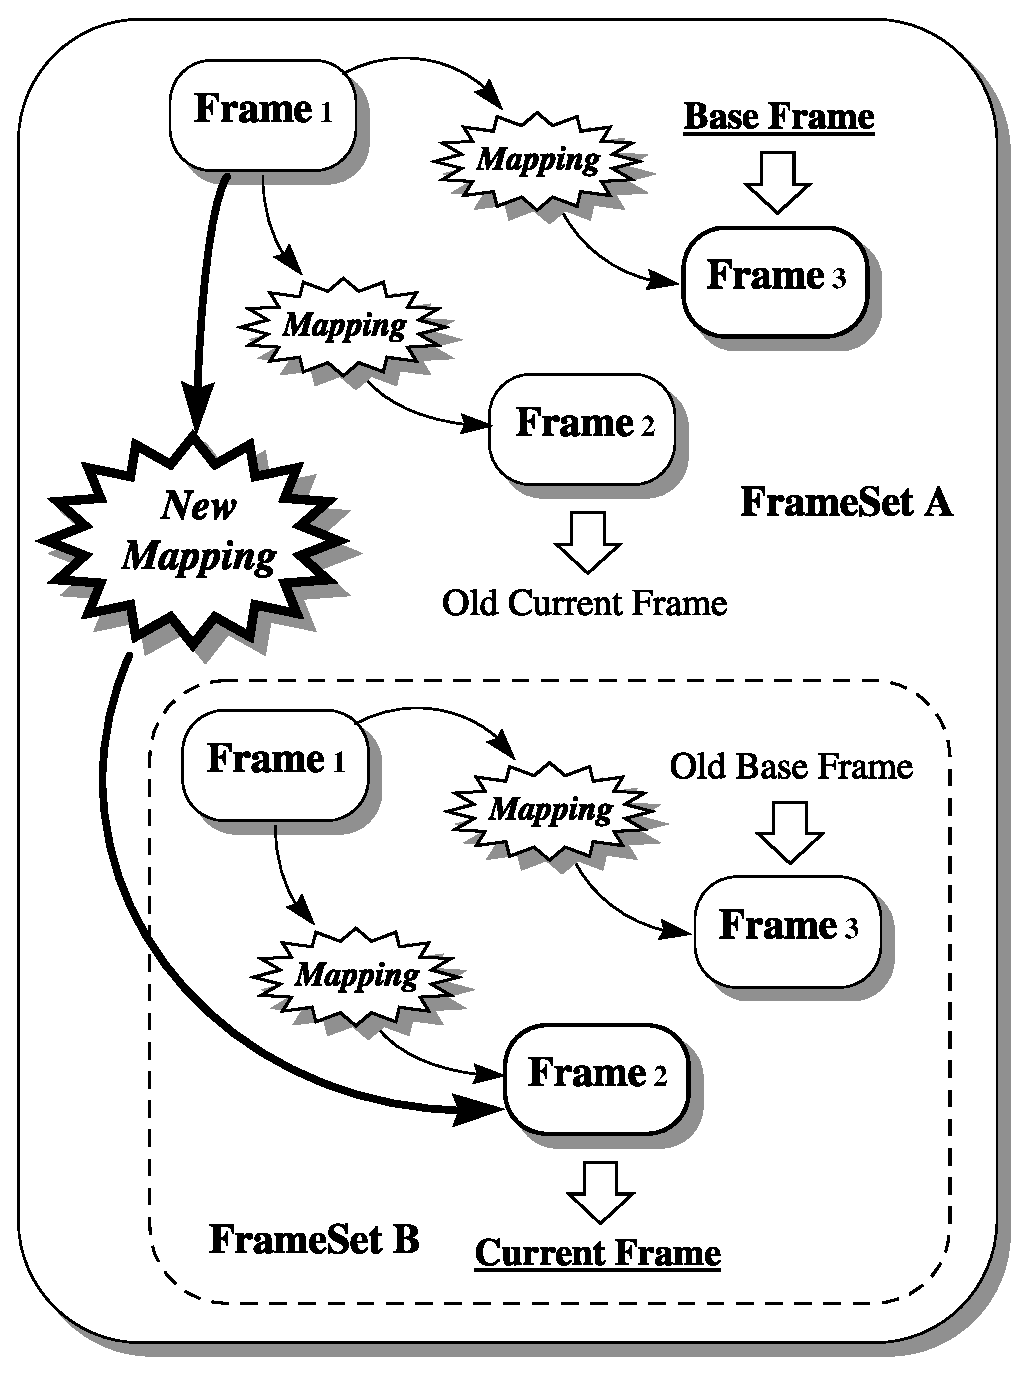
\includegraphics[scale=0.6]{sun210_figures/fsmerge.eps}
   \caption{Two FrameSets in the process of being merged using
   \htmlref{AST\_ADDFRAME}{AST_ADDFRAME}. FrameSet~B is being added to FrameSet~A by supplying a
   new \htmlref{Mapping}{Mapping} which inter-relates a nominated \htmlref{Frame}{Frame} in A (here number~1)
   and the current Frame of B. In the merged FrameSet, the Frames
   contributed by B will be re-numbered to become Frames~4, 5 and 6. The
   base Frame will remain unchanged, but the current Frame of B becomes
   the new current Frame. Note that FrameSet~B itself is not
   altered by this process.}
   \label{fig:fsmerge}
   \end{center}
   \end{figure}
\end{latexonly}
\begin{htmlonly}
   As well as adding individual Frames to a FrameSet
   (\secref{ss:addingframes}), it is also possible to add complete sets of
   inter-related Frames which are contained within another
   FrameSet. This, of course, corresponds to the process of merging two
   FrameSets (see Figure below).
   \begin{quote}
   \begin{figure}[hbtp]
   \label{fig:fsmerge}
   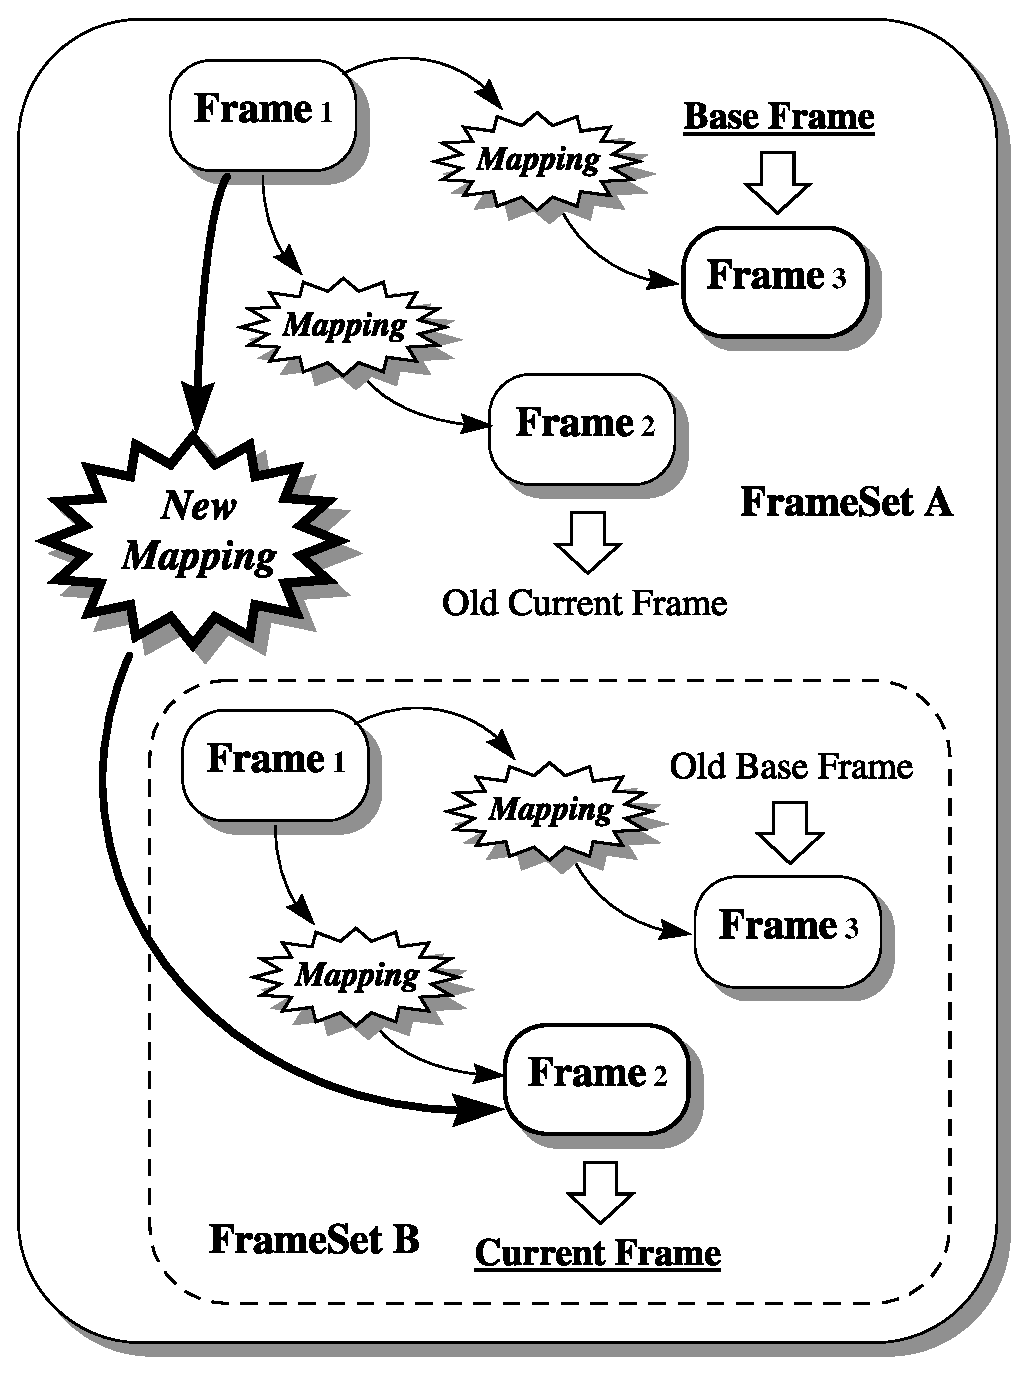
\includegraphics[scale=0.75]{sun210_figures/fsmerge.eps}
   \caption{Two FrameSets in the process of being merged using
   AST\_ADDFRAME. FrameSet~B is being added to FrameSet~A by supplying a
   new Mapping which inter-relates a nominated Frame in A (here number~1)
   and the current Frame of B. In the merged FrameSet, the Frames
   contributed by B will be re-numbered to become Frames~4, 5 and 6. The
   base Frame will remain unchanged, but the current Frame of B becomes
   the new current Frame. Note that FrameSet~B itself is not
   altered by this process.}
   \end{figure}
   \end{quote}
\end{htmlonly}

This process is performed by adding one FrameSet to another using
AST\_ADDFRAME, in much the same manner as when adding a new Frame to
an existing FrameSet (\secref{ss:addingframes}). It is simply a matter
of providing a FrameSet pointer, instead of a Frame pointer, for the
4th argument. In performing the merger you must, as usual, supply a
Mapping, but in this case the Mapping should relate the current Frame
of the FrameSet being added to one of the Frames already present. For
example, you might perform the merger shown in
Figure~\ref{fig:fsmerge} as follows:

\small
\begin{verbatim}
      INTEGER MAPPING

      ...

      CALL AST_ADDFRAME( FRAMESETA, 1, MAPPING, FRAMESETB, STATUS )
\end{verbatim}
\normalsize

The Frames acquired by FRAMESETA from the FrameSet being added
(FRAMESETB) are re-numbered so that they retain their original order
and follow on consecutively after the Frames that were already
present, whose indices remain unchanged. The base Frame of FRAMESETA
remains unchanged, but the current Frame of FRAMESETB becomes its new
current Frame. All the inter-relationships between Frames in both
FrameSets remain in place and are preserved in the merged FrameSet.

Note that while this process modifies the first FrameSet (FRAMESETA),
it leaves the original contents of the one being added (FRAMESETB)
unchanged.

%\cleardoublepage
%\section{\label{ss:searching}TBW - Searching for Coordinate Systems}

\cleardoublepage
\section{\label{ss:channels}Saving and Restoring Objects (Channels)}

Facilities are provided by the AST library for performing input and
output (I/O) with any kind of \htmlref{Object}{Object}. This means it is possible
to write any Object into various external representations for
storage, and then to read these representations back in, so as to
restore the original Object. Typically, an Object would be written by
one program and read back in by another.

We refer to ``external representations'' in the plural because AST is
designed to function independently of any particular data storage
system. This means that Objects may need converting into a number of
different external representations in order to be compatible with
(say) the astronomical data storage system in which they will reside.

In this section, we discuss the basic I/O facilities which support
external representations based on a textual format referred to as the AST
``native format''. These are implemented using a new kind of Object---a
\htmlref{Channel}{Channel}. We will examine later how to use other representations, based on
an XML format or on the use of FITS headers, for storing Objects. These
are implemented using more specialised forms of Channel called \htmlref{XmlChan}{XmlChan}
(\secref{ss:xmlchan}) and \htmlref{FitsChan}{FitsChan} (\secref{ss:nativefits}).

\subsection{The Channel Model}

The best way to start thinking about a \htmlref{Channel}{Channel} is like a Fortran I/O
unit (also represented by an integer, as it happens) and to think of
the process of creating a Channel as the combined process of
allocating a unit number and attaching it to a file by opening the
file on that unit. Subsequently, you can read and write Objects
{\em{via}} the Channel.

This analogy is not quite perfect, however, because a Channel has, in
principle, two ``files'' attached to it. One is used when reading, and
the other when writing. These are termed the Channel's {\em{source}}
and {\em{sink}} respectively. In practice, the source and sink may
both be the same, in which case the analogy with the Fortran I/O unit
is correct, but this need not always be so. It is not necessarily so
with the basic Channel, as we will now see
(\secref{ss:creatingachannel}).

\subsection{\label{ss:creatingachannel}Creating a Channel}

The process of creating a \htmlref{Channel}{Channel} is straightforward. As you
might expect, it uses the constructor function \htmlref{AST\_CHANNEL}{AST_CHANNEL}:

\small
\begin{verbatim}
      INCLUDE 'AST_PAR'
      INTEGER CHANNEL, STATUS

      STATUS = 0

      ...

      CHANNEL = AST_CHANNEL( AST_NULL, AST_NULL, ' ', STATUS )
\end{verbatim}
\normalsize

The first two arguments to AST\_CHANNEL specify the external source
and sink that the Channel is to use. There arguments are the names of
Fortran subroutines and we will examine their use in more detail later
(\secref{ss:channelsource} and \secref{ss:channelsink}).

In this very simple example we have supplied the name of the null
routine AST\_NULL\footnote{Note that AST\_NULL (one underscore) is a
routine name and is distinct from AST\_\_NULL (two underscores) which
is a null \htmlref{Object}{Object} pointer.  Since we are passing the name of one
routine to another routine, AST\_NULL would normally have to appear in
a Fortran EXTERNAL statement. In this example, however, a suitable
statement is already present in the AST\_PAR include file.} for both
the source and sink routines.  This requests the default behaviour,
which means that textual input will be read from the program's
standard input stream (typically, this means your keyboard) while
textual output will go to the standard output stream (typically
appearing on your screen). On UNIX systems, of course, either of these
streams can easily be redirected to files.

\subsection{\label{ss:writingtoachannel}Writing Objects to a Channel}

The process of saving Objects is very straightforward. You can
simply write any \htmlref{Object}{Object} to a \htmlref{Channel}{Channel} using the \htmlref{AST\_WRITE}{AST_WRITE}
function, as follows:

\small
\begin{verbatim}
      INTEGER NOBJ, OBJECT

      ...

      NOBJ = AST_WRITE( CHANNEL, OBJECT, STATUS )
\end{verbatim}
\normalsize

The effect of this will be to produce a textual description of the
Object which will appear, by default, on your program's standard
output stream. Any class of Object may be converted into text in this
way.

AST\_WRITE returns a count of the number of Objects written. Usually,
this will be one, unless the Object supplied cannot be
represented. With a basic Channel all Objects can be represented, so a
value of one will always be returned unless there has been an
error. We will see later, however, that more specialised forms of
Channel may impose restrictions on the kind of Object you can write
(\secref{ss:foreignfitslimitations}). In such cases, AST\_WRITE may
return zero to indicate that the Object was not acceptable.

\subsection{\label{ss:readingfromachannel}Reading Objects from a Channel}

Before discussing the format of the output produced above
(\secref{ss:writingtoachannel}), let us consider how to read it back,
so as to reconstruct the original \htmlref{Object}{Object}. Naturally, we would first
need to save the output in a file. We can do that either by using the
\htmlref{SinkFile}{SinkFile} attribute, or (on UNIX systems), by redirecting standard output
to a file using a shell command like:

\begin{quote}
\small
\begin{verbatim}
program1 >file
\end{verbatim}
\normalsize
\end{quote}

Within a subsequent program, we can read this Object back in by
using the \htmlref{AST\_READ}{AST_READ} function, having first created a suitable
\htmlref{Channel}{Channel}:

\small
\begin{verbatim}
      OBJECT = AST_READ( CHANNEL, STATUS )
\end{verbatim}
\normalsize

By default, this function will read from the standard input stream
(the default source for a basic Channel), so we would need to ensure
that our second program reads its input from the file in which the
Object description is stored. On UNIX systems, we could again use a
shell redirection command such as:

\begin{quote}
\small
\begin{verbatim}
program2 <file
\end{verbatim}
\normalsize
\end{quote}

Alternatively, we could have assigned a value to the SinkFile attribute
before invoking
AST\_READ.

\subsection{Saving and Restoring Multiple Objects}

I/O operations performed on a basic \htmlref{Channel}{Channel} are sequential. This
means that if you write more than one \htmlref{Object}{Object} to a Channel,
each new Object's textual description is simply appended to the
previous one. You can store any number of Objects in this way,
subject only to the storage space you have available.

After you read an Object back from a basic Channel, the
Channel is ``positioned'' at the end of that Object's
textual description. If you then perform another read, you will
read the next Object's textual description and therefore
retrieve the next Object.  This process may be repeated to read
each Object in turn. When there are no more Objects to be
read, \htmlref{AST\_READ}{AST_READ} will return the value AST\_\_NULL to indicate an
{\em{end-of-file.}}

\subsection{\label{ss:validatinginput}Validating Input}

The pointer returned by \htmlref{AST\_READ}{AST_READ} (\secref{ss:readingfromachannel})
could identify any class of \htmlref{Object}{Object}---this is determined entirely by
the external data being read. If it is necessary to test for a
particular class (say a \htmlref{Frame}{Frame}), this may be done as follows using the
appropriate member of the \htmlref{AST\_ISA$<$CLASS$>$}{AST_ISACLASS} family of functions:

\small
\begin{verbatim}
      LOGICAL OK

      ...

      OK = AST_ISAFRAME( OBJECT, STATUS )
\end{verbatim}
\normalsize

Note, however, that this will accept any Frame, so would be equally
happy with a basic Frame or a \htmlref{SkyFrame}{SkyFrame}.  An alternative validation
strategy would be to obtain the value of the Object's \htmlref{Class}{Class} attribute
and then test this character string, as follows:

\small
\begin{verbatim}
      OK = AST_GETC( OBJECT, 'Class', STATUS ) .EQ. 'Frame'
\end{verbatim}
\normalsize

This would only accept a basic Frame and would reject a SkyFrame.

\subsection{Storing an ID String with an Object}

Occasionally, you may want to store a number of Objects and later
retrieve them and use each for a different purpose. If the Objects are
of the same class, you cannot use the \htmlref{Class}{Class} attribute to distinguish
them when you read them back
({\em{c.f.}}~\secref{ss:validatinginput}). Although relying on the
order in which they are stored is a possible solution, this becomes
complicated if some of the Objects are optional and may not always be
present. It also makes extending your data format in future more
difficult.

To help with this, every AST \htmlref{Object}{Object} has an \htmlref{ID}{ID} attribute and an \htmlref{Ident}{Ident}
attribute, both of which allows you, in effect, to attach a textual
identification label to it. You simply set the ID or Ident attribute before
writing the Object:

\small
\begin{verbatim}
      CALL AST_SET( OBJECT, 'ID=Calibration', STATUS )
      NOBJ = AST_WRITE( CHANNEL, OBJECT, STATUS )
\end{verbatim}
\normalsize

You can then test its value after you read the Object back:

\small
\begin{verbatim}
      OBJECT = AST_READ( CHANNEL, STATUS )
      IF ( AST_GETC( OBJECT, 'ID', STATUS ) .EQ. 'Calibration' ) THEN
         <the Calibration Object has been read>
      ELSE
         <some other Object has been read>
      END IF
\end{verbatim}
\normalsize

The only difference between the ID and Ident attributes is that the ID
attribute is unique to a particular Object and is lost if, for example,
you make a copy of the Object. The Ident attrubute, on the other hand, is
transferred to the new Object when a copy is made. Consequently, it is
safest to set the value of the ID attribute immediately before you
perform the write.

\subsection{\label{ss:textualoutputformat}The Textual Output Format}

Let us now examine the format of the textual output produced by
writing an \htmlref{Object}{Object} to a basic \htmlref{Channel}{Channel}
(\secref{ss:writingtoachannel}). To give a concrete example, suppose
the Object in question is a \htmlref{SkyFrame}{SkyFrame}, written out as follows:

\small
\begin{verbatim}
      INTEGER SKYFRAME

      ...

      NOBJ = AST_WRITE( CHANNEL, SKYFRAME, STATUS )
\end{verbatim}
\normalsize

The output should then look like the following:

\begin{quote}
\small
\begin{verbatim}
 Begin SkyFrame 	# Description of celestial coordinate system
#   Title = "FK4 Equatorial Coordinates, no E-terms, Mean Equinox B1950.0, Epoch B1958.0" 	# Title of coordinate system
    Naxes = 2 	# Number of coordinate axes
#   Domain = "SKY" 	# Coordinate system domain
#   Lbl1 = "Right Ascension" 	# Label for axis 1
#   Lbl2 = "Declination" 	# Label for axis 2
#   Uni1 = "hh:mm:ss.s" 	# Units for axis 1
#   Uni2 = "ddd:mm:ss" 	# Units for axis 2
#   Dir1 = 0 	# Plot axis 1 in reverse direction (hint)
    Ax1 = 	# Axis number 1
       Begin SkyAxis 	# Celestial coordinate axis
       End SkyAxis
    Ax2 = 	# Axis number 2
       Begin SkyAxis 	# Celestial coordinate axis
       End SkyAxis
 IsA Frame 	# Coordinate system description
    System = "FK4-NO-E" 	# Celestial coordinate system type
    Epoch = 1958 	# Besselian epoch of observation
#   Eqnox = 1950 	# Besselian epoch of mean equinox
 End SkyFrame
\end{verbatim}
\normalsize
\end{quote}

You will notice that this output is designed both for a human reader,
in that it is formatted, and also to be read back by a computer in
order to reconstruct the SkyFrame. In fact, this is precisely the way
that \htmlref{AST\_SHOW}{AST_SHOW} works (\secref{ss:displayingobjects}), this routine
being roughly equivalent to the following use of a Channel:

\small
\begin{verbatim}
      CHANNEL = AST_CHANNEL( AST_NULL, AST_NULL, ' ', STATUS )
      NOBJ = AST_WRITE( CHANNEL, OBJECT, STATUS )
      CALL AST_ANNUL( CHANNEL, STATUS )
\end{verbatim}
\normalsize

Some lines of the output start with a ``\verb?#?'' comment character,
which turns the rest of the line into a comment. These lines will be
ignored when read back in by \htmlref{AST\_READ}{AST_READ}.  They typically contain
default values, or values that can be derived in some way from the
other data present, so that they do not actually need to be stored in
order to reconstruct the original Object. They are provided purely for
human information. The same comment character is also used to append
explanatory comments to most output lines.

It is not sensible to attempt a complete description of this output
format because every class of Object is potentially different and each
can define how its own data should be represented. However, there are
some basic rules, which mean that the following common features will
usually be present:

\begin{enumerate}
\item Each Object is delimited by matching ``Begin'' and ``End''
lines, which also identify the class of Object involved.

\item Within each Object description, data values are represented
by a simple ``keyword~$=$~value'' syntax, with one value to a line.

\item Lines beginning ``IsA'' are used to mark the divisions between
data belonging to different levels in the class hierarchy
(\appref{ss:classhierarchy}). Thus, ``IsA~\htmlref{Frame}{Frame}'' marks the end of data
associated with the Frame class and the start of data associated with
some derived class (a SkyFrame in the above example). ``IsA'' lines
may be omitted if associated data values are absent and no confusion
arises.

\item Objects may contain other Objects as data. This is
indicated by an absent value, with the description of the data
Object following on subsequent lines.

\item Indentation is used to clarify the overall structure.
\end{enumerate}

Beyond these general principles, the best guide to what a particular
line of output represents will generally be the comment which
accompanies it together with a general knowledge of the class of
Object being described.

\subsection{\label{ss:controllingchanneloutput}Controlling the Amount of Output}

It is not always necessary for the output from \htmlref{AST\_WRITE}{AST_WRITE}
(\secref{ss:writingtoachannel}) to be human-readable, so a \htmlref{Channel}{Channel} has
attributes that allow the amount of detail in the output to be
controlled.

The first of these is the integer attribute \htmlref{Full}{Full}, which controls the
extent to which optional, commented out, output lines are produced. By
default, Full is zero, and this results in the standard style of
output (\secref{ss:textualoutputformat}) where default values that may
be helpful to humans are included. To suppress these optional lines,
Full should be set to $-$1. This is most conveniently done when the
Channel is created, so that:

\small
\begin{verbatim}
      CHANNEL = AST_CHANNEL( AST_NULL, AST_NULL, 'Full=-1', STATUS )
      NOBJ = AST_WRITE( CHANNEL, SKYFRAME, STATUS )
      CALL AST_ANNUL( CHANNEL, STATUS )
\end{verbatim}
\normalsize

would result in output containing only the essential information, such
as:

\begin{quote}
\small
\begin{verbatim}
 Begin SkyFrame 	# Description of celestial coordinate system
    Naxes = 2 	# Number of coordinate axes
    Ax1 = 	# Axis number 1
       Begin SkyAxis 	# Celestial coordinate axis
       End SkyAxis
    Ax2 = 	# Axis number 2
       Begin SkyAxis 	# Celestial coordinate axis
       End SkyAxis
 IsA Frame 	# Coordinate system description
    System = "FK4-NO-E" 	# Celestial coordinate system type
    Epoch = 1958 	# Besselian epoch of observation
 End SkyFrame
\end{verbatim}
\normalsize
\end{quote}

In contrast, setting Full to $+$1 will result in additional output
lines which will reveal every last detail of the \htmlref{Object}{Object}'s
construction. Often this will be rather more than you want, especially
for more complex Objects, but it can sometimes help when debugging
programs. This is how a \htmlref{SkyFrame}{SkyFrame} appears at this level of detail:

\begin{quote}
\small
\begin{verbatim}
 Begin SkyFrame 	# Description of celestial coordinate system
#   RefCnt = 1 	# Count of active Object pointers
#   Nobj = 1 	# Count of active Objects in same class
 IsA Object 	# Astrometry Object
#   Nin = 2 	# Number of input coordinates
#   Nout = 2 	# Number of output coordinates
#   Invert = 0 	# Mapping not inverted
#   Fwd = 1 	# Forward transformation defined
#   Inv = 1 	# Inverse transformation defined
#   Report = 0 	# Don't report coordinate transformations
 IsA Mapping 	# Mapping between coordinate systems
#   Title = "FK4 Equatorial Coordinates, no E-terms, Mean Equinox B1950.0, Epoch B1958.0" 	# Title of coordinate system
    Naxes = 2 	# Number of coordinate axes
#   Domain = "SKY" 	# Coordinate system domain
#   Lbl1 = "Right Ascension" 	# Label for axis 1
#   Lbl2 = "Declination" 	# Label for axis 2
#   Sym1 = "RA" 	# Symbol for axis 1
#   Sym2 = "Dec" 	# Symbol for axis 2
#   Uni1 = "hh:mm:ss.s" 	# Units for axis 1
#   Uni2 = "ddd:mm:ss" 	# Units for axis 2
#   Dig1 = 7 	# Individual precision for axis 1
#   Dig2 = 7 	# Individual precision for axis 2
#   Digits = 7 	# Default formatting precision
#   Fmt1 = "hms.1" 	# Format specifier for axis 1
#   Fmt2 = "dms" 	# Format specifier for axis 2
#   Dir1 = 0 	# Plot axis 1 in reverse direction (hint)
#   Dir2 = 1 	# Plot axis 2 in conventional direction (hint)
#   Presrv = 0 	# Don't preserve target axes
#   Permut = 1 	# Axes may be permuted to match
#   MinAx = 2 	# Minimum number of axes to match
#   MaxAx = 2 	# Maximum number of axes to match
#   MchEnd = 0 	# Match initial target axes
#   Prm1 = 1 	# Axis 1 not permuted
#   Prm2 = 2 	# Axis 2 not permuted
    Ax1 = 	# Axis number 1
       Begin SkyAxis 	# Celestial coordinate axis
#         RefCnt = 1 	# Count of active Object pointers
#         Nobj = 2 	# Count of active Objects in same class
       IsA Object 	# Astrometry Object
#         Label = "Angle on Sky" 	# Axis Label
#         Symbol = "delta" 	# Axis symbol
#         Unit = "ddd:mm:ss" 	# Axis units
#         Digits = 7 	# Default formatting precision
#         Format = "dms" 	# Format specifier
#         Dirn = 1 	# Plot in conventional direction
       IsA Axis 	# Coordinate axis
#         Format = "dms" 	# Format specifier
#         IsLat = 0 	# Longitude axis (not latitude)
#         AsTime = 0 	# Display values as angles (not times)
       End SkyAxis
    Ax2 = 	# Axis number 2
       Begin SkyAxis 	# Celestial coordinate axis
#         RefCnt = 1 	# Count of active Object pointers
#         Nobj = 2 	# Count of active Objects in same class
       IsA Object 	# Astrometry Object
#         Label = "Angle on Sky" 	# Axis Label
#         Symbol = "delta" 	# Axis symbol
#         Unit = "ddd:mm:ss" 	# Axis units
#         Digits = 7 	# Default formatting precision
#         Format = "dms" 	# Format specifier
#         Dirn = 1 	# Plot in conventional direction
       IsA Axis 	# Coordinate axis
#         Format = "dms" 	# Format specifier
#         IsLat = 0 	# Longitude axis (not latitude)
#         AsTime = 0 	# Display values as angles (not times)
       End SkyAxis
 IsA Frame 	# Coordinate system description
    System = "FK4-NO-E" 	# Celestial coordinate system type
    Epoch = 1958 	# Besselian epoch of observation
#   Eqnox = 1950 	# Besselian epoch of mean equinox
 End SkyFrame
\end{verbatim}
\normalsize
\end{quote}

\subsection{\label{ss:channelcommenting}Controlling Commenting}

Another way of controlling output from a \htmlref{Channel}{Channel} is {\em{via}} the
boolean (integer) \htmlref{Comment}{Comment} attribute, which controls whether comments
are appended to describe the purpose of each value. Comment has the
value 1 by default but, if set to zero, will suppress these
comments. This is normally appropriate only if you wish to minimise
the amount of output, for example:

\small
\begin{verbatim}
      CALL AST_SET( CHANNEL, 'Full=-1, Comment=0', STATUS )
      NOBJ = AST_WRITE( CHANNEL, SKYFRAME, STATUS )
\end{verbatim}
\normalsize

might result in the following more compact output:

\begin{quote}
\small
\begin{verbatim}
 Begin SkyFrame
    Naxes = 2
    Ax1 =
       Begin SkyAxis
       End SkyAxis
    Ax2 =
       Begin SkyAxis
       End SkyAxis
 IsA Frame
    System = "FK4-NO-E"
    Epoch = 1958
 End SkyFrame
\end{verbatim}
\normalsize
\end{quote}

\subsection{Editing Textual Output}

The safest advice about editing the textual output from \htmlref{AST\_WRITE}{AST_WRITE} (or
\htmlref{AST\_SHOW}{AST_SHOW}) is ``don't!''---unless you know what you are doing.

Having given that warning, however, it is sometimes possible to make
changes to the text, or even to write entire \htmlref{Object}{Object} descriptions from
scratch, and to read the results back in to construct new
Objects. Normally, simple changes to numerical values are safest, but
be aware that this is a back door method of creating Objects, so
you are on your own! There are a number of potential pitfalls. In
particular:

\begin{itemize}
\item \htmlref{AST\_READ}{AST_READ} is intended for retrieving data written by AST\_WRITE
and not for reading data input by humans. As such, the data validation
provided is very limited and is certainly not foolproof. This makes it
quite easy to construct Objects that are internally inconsistent by
this means. In contrast, the normal programming interface incorporates
numerous checks designed to make it impossible to construct invalid
Objects. You should not necessarily think you have found a bug if your
changes to an Object's textual description fail to produce the results
you expected!

\item In many instances the names associated with values in textual
output will correspond with Object attributes. Sometimes, however,
these names may differ from the attribute name. This is mainly because
of length restrictions imposed by other common external formats, such
as FITS headers. Some of the names used do not correspond with
attributes at all.

\item It is safest to change single numerical or string values.
Beware of changing the size or shape of Objects ({\em{e.g.}}\ the
number of axes in a \htmlref{Frame}{Frame}). Often, these values must match others
stored elsewhere within the Object and changing them in a haphazard
fashion will not produce useful results.

\item Be wary about un-commenting default values. Sometimes this will
work, but often these values are derived from other Objects stored
more deeply in the structure and the proper place to insert a new
value is not where the default itself appears.
\end{itemize}

\subsection{\label{ss:mixingchanneltext}Mixing Objects with other Text}

By default, when you use \htmlref{AST\_READ}{AST_READ} to read from a basic \htmlref{Channel}{Channel}
(\secref{ss:readingfromachannel}), it is assumed that you are reading a
stream of text containing only AST Objects, which follow each other
end-to-end. If any extraneous input data are encountered which do not
appear to form part of the textual description of an \htmlref{Object}{Object}, then an
error will result. In particular, the first input line must identify
the start of an Object description, so you cannot start reading half
way through an Object.

Sometimes, however, you may want to store AST Object descriptions
intermixed with other textual data. You can do this by setting the
Channel's boolean (integer) \htmlref{Skip}{Skip} attribute to 1. This will cause every
read to skip over extraneous data until the start of a new AST Object
description, if any, is found. So long as your other data do not mimic
the appearance of an AST Object description, the two sets of data can
co-exist.

For example, by setting Skip to 1, the following complete Fortran
program will read all the AST Objects whose descriptions appear in the
source of this document, ignoring the other text. \htmlref{AST\_SHOW}{AST_SHOW} is used to
display those found:

\small
\begin{verbatim}
      INCLUDE 'AST_PAR'
      INTEGER CHANNEL, OBJECT, STATUS

      STATUS = 0
      CHANNEL = AST_CHANNEL( AST_NULL, AST_NULL, 'Skip=1', STATUS )
 1    OBJECT = AST_READ( CHANNEL, STATUS )
      IF ( OBJECT .NE. AST__NULL ) THEN
         CALL AST_SHOW( OBJECT, STATUS )
         CALL AST_ANNUL( OBJECT, STATUS )
         GO TO 1
      END IF
      CALL AST_ANNUL( CHANNEL, STATUS )
      END
\end{verbatim}
\normalsize

\subsection{\label{ss:channelsource}Reading Objects from Files}

Thus far, we have only considered the default behaviour of a \htmlref{Channel}{Channel}
in reading and writing Objects through a program's standard input and
output streams. We will now consider how to access Objects stored in
files more directly.

The simple approach is to use the \htmlref{SinkFile}{SinkFile} and \htmlref{SourceFile}{SourceFile} attributes of
the Channel. For instance, the following will read a pair of Objects from
a text file called ``fred.txt'':

\small
\begin{verbatim}
   CALL AST_SET( CHANNEL, 'SourceFile=fred.txt', STATUS )
   OBJ1 = AST_READ( CHANNEL, STATUS )
   OBJ2 = AST_READ( CHANNEL, STATUS )
   CALL AST_CLEAR( CHANNEL, 'SourceFile', STATUS )
\end{verbatim}
\normalsize

Note, the act of clearing the attribute tells AST that no more Objects
are to be read from the file and so the file is then closed. If the
attribute is not cleared, the file will remain open and further Objects
can be read from it. The file will always be closed when the Channel is
deleted.

This simple approach will normally be sufficient. However, because the
AST library is designed to be used from more than one language, it has
to be a little careful about reading and writing to files. This is due
to incompatibilities that may exist between the file I/O facilities
provided by different languages. If such incompatibilities prevent the
above simple system being used, we need to adopt a system that off-loads
all file I/O to external code.

What this means in practice is that if the above simple approach cannot
be used, you must instead provide some simple
Fortran routines that perform the actual transfer of data to and from
files and similar external data stores. The routines you provide are
supplied as the source and/or sink routine arguments to \htmlref{AST\_CHANNEL}{AST_CHANNEL}
when you create a Channel (\secref{ss:creatingachannel}). An example is
the best way to illustrate this.

Consider the following simple subroutine called SOURCE. It reads a
single line of text from a Fortran I/O unit and then calls
\htmlref{AST\_PUTLINE}{AST_PUTLINE} to pass it to the AST library, together with its
length. It sets this length to be negative if there is no more input:

\small
\begin{verbatim}
      SUBROUTINE SOURCE( STATUS )
      INTEGER STATUS
      CHARACTER * ( 200 ) BUFFER

      READ( 1, '(A)', END = 99 ) BUFFER
      CALL AST_PUTLINE( BUFFER, LEN( BUFFER ), STATUS )
      RETURN

 99   CALL AST_PUTLINE( BUFFER, -1, STATUS )
      END
\end{verbatim}
\normalsize

Our main program might then look something like this (omitting error
checking for brevity):

\small
\begin{verbatim}
      EXTERNAL SOURCE

      ...

*  Open the input file.
      OPEN( UNIT = 1, FILE = 'infile.ast', STATUS = 'OLD' )

*  Create the Channel and read an Object from it.
      CHANNEL = AST_CHANNEL( SOURCE, AST_NULL, ' ', STATUS )
      OBJECT = AST_READ( CHANNEL, STATUS )

      ...

*  Annul the Channel and close the file when done.
      CALL AST_ANNUL( CHANNEL, STATUS )
      CLOSE( 1 )
\end{verbatim}
\normalsize

Here, we first open the required input file.  We then pass the name of
our SOURCE routine as the first argument to AST\_CHANNEL when creating
a new Channel (ensuring that SOURCE also appears in an EXTERNAL
statement). When we read an \htmlref{Object}{Object} from this Channel using
\htmlref{AST\_READ}{AST_READ}, the SOURCE routine will be called to obtain the textual
data from the file, the end-of-file being detected when it yields a
negative line length.

Note, if a value is set for the SourceFile attribute,
the AST\_READ function will ignore any source routine
specified when the Channel was created.

\subsection{\label{ss:channelsink}Writing Objects to Files}

As for reading, writing Objects to files can be done in two different ways.
Again, the simple approach is to use the \htmlref{SinkFile}{SinkFile} attribute of the \htmlref{Channel}{Channel}.
For instance, the following will write a pair of Objects to a text file
called ``fred.txt'':

\small
\begin{verbatim}
   CALL AST_SET( CHANNEL, 'SinkFile=fred.txt', STATUS )
   NOBJ = AST_WRITE( CHANNEL, OBJECT1, STATUS )
   NOBJ = AST_WRITE( CHANNEL, OBJECT2, STATUS )
   CALL AST_CLEAR( CHANNEL, 'SinkFile', STATUS )
\end{verbatim}
\normalsize

Note, the act of clearing the attribute tells AST that no more output
will be written to the file and so the file is then closed. If the
attribute is not cleared, the file will remain open and further Objects
can be written to it. The file will always be closed when the Channel is
deleted.

If the details of the language's I/O system on the computer you are using
means that the above approach cannot be used, then we can write a SINK routine,
that obtains a line of output text from the AST library by calling \htmlref{AST\_GETLINE}{AST_GETLINE}
and then writes it to a file. We can use this in basically the same way as
the SOURCE routine in the previous section (\secref{ss:channelsource}):

\small
\begin{verbatim}
      SUBROUTINE SINK( STATUS )
      INTEGER L, STATUS
      CHARACTER * ( 200 ) BUFFER

      CALL AST_GETLINE( BUFFER, L, STATUS )
      IF ( L .GT. 0 ) WRITE( 2, '(A)' ) BUFFER( : L )

      END
\end{verbatim}
\normalsize

In this case, our main program would supply the name of this SINK
routine as the second argument to \htmlref{AST\_CHANNEL}{AST_CHANNEL} (ensuring that it also
appears in an EXTERNAL statement), as follows:

\small
\begin{verbatim}
      EXTERNAL SINK

      ...

*  Open the output file.
      OPEN( UNIT = 2, FILE = 'outfile.ast', STATUS = 'NEW' )

*  Create a Channel and write an Object to it.
      CHANNEL = AST_CHANNEL( SOURCE, SINK, ' ', STATUS )
      NOBJ = AST_WRITE( CHANNEL, OBJECT, STATUS )

      ...

*  Annul the Channel and close the file when done.
      CALL AST_ANNUL( CHANNEL, STATUS )
      CLOSE( 2 )
\end{verbatim}
\normalsize

Note that we can specify a source and/or a sink routine for the
Channel, and that these may use either the same file, or different
files according to whether we are reading or writing. AST has no
knowledge of the underlying file system, nor of file positioning. It
just reads and writes sequentially. If you wish, for example, to
reposition a file at the beginning in between reads and writes, then
this can be done directly (and completely independently of AST) using
standard Fortran statements.

If an error occurs in your source or sink routine, you can communicate
this to the AST library by setting the STATUS argument to any error
value. This will immediately terminate the read or write operation.

Note, if a value is set for the SinkFile attribute,
the \htmlref{AST\_WRITE}{AST_WRITE} function will ignore any sink routine
specified when the Channel was created.

\subsection{\label{ss:otherplaces}Reading and Writing Objects to other Places}

It should be obvious from the above (\secref{ss:channelsource} and
\secref{ss:channelsink}) that a \htmlref{Channel}{Channel}'s source and sink routines
provide a flexible means of intercepting textual data that describes
AST Objects as it flows in and out of your program. In fact, you might
like to regard a Channel simply as a filter for converting AST Objects
to and from a stream of text which is then handled by your source and
sink routines, where the real I/O occurs.

This gives you the ability to store AST Objects in virtually any data
system, so long as you can convert a stream of text into something
that can be stored (it need no longer be text) and retrieve it
again. There is generally no need to retain comments.  Other
possibilities, such as inter-process and network communication, could
also be implemented {\em{via}} source and sink functions in basically
the same way.

\cleardoublepage
\section{\label{ss:nativefits}Storing AST Objects in FITS Headers (FitsChans)}

\begin{latexonly}
A FITS header is a sequence of 80-character strings, formatted
according to particular rules defined by the Flexible Image Transport
\htmlref{System}{System}
(FITS). FITS\footnote{http://fits.gsfc.nasa.gov/}
is a widely-used standard for data interchange in astronomy and has
also been adopted as a data processing format in some astronomical
data reduction systems.  The individual 80-character strings in a FITS
header are usually called {\em{cards}} or {\em{header cards}} (for
entirely anachronistic reasons).
\end{latexonly}
\begin{htmlonly}
A FITS header is a sequence of 80-character strings, formatted
according to particular rules defined by the Flexible Image Transport
System (FITS).
\htmladdnormallink{FITS}{http://fits.gsfc.nasa.gov/}
is a widely-used standard for data interchange in astronomy and has
also been adopted as a data processing format in some astronomical
data reduction systems.  The individual 80-character strings in a FITS
header are usually called {\em{cards}} or {\em{header cards}} (for
entirely anachronistic reasons).
\end{htmlonly}

A sequence of FITS cards appears as a header at the start of every
FITS data file, and sometimes also at other points within it, and is
used to provide ancillary information which qualifies or describes the
main array of data stored in the file. As such, FITS headers are prime
territory for storing information about the coordinate systems
associated with data held in FITS files.

In this section, we will examine how to store information in FITS
headers directly in the form of AST Objects---a process which is
supported by a specialised class of \htmlref{Channel}{Channel} called a \htmlref{FitsChan}{FitsChan}. Our
discussion here will turn out to be a transitional step that
emphasises the similarities between a FitsChan and a Channel
(\secref{ss:channels}). At the same time, it will prepare us for the
next section (\secref{ss:foreignfits}), where we will examine how to
use a FitsChan to tackle some of the more difficult problems that FITS
headers can present.

\subsection{\label{ss:nativeencoding}The Native FITS Encoding}

As it turns out, we are not the first to have thought of storing WCS
information in FITS headers. In fact, the original FITS standard (1981
vintage) defined a set of header keywords for this purpose which have
been widely used, although they have proved too limited for many
practical purposes.

At the time of writing, a number of different ways of using FITS
headers for storing WCS information are in use, most (although not
all) based on the original standard. We will refer to these
alternative ways of storing the information as FITS {\em{encodings}}
but will defer a discussion of their advantages and limitations until
the next section (\secref{ss:foreignfits}).

Here, we will examine how to store AST Objects directly in FITS
headers. In effect, this defines a new encoding, which we will term
the {\em{native encoding.}} This is a special kind of encoding,
because not only does it allow us to associate conventional
WCS calibration information with FITS data, but it also allows any other
information that can be expressed in terms of AST Objects to be stored
as well.  In fact, the native encoding provides us with facilities
roughly analogous to those of the \htmlref{Channel}{Channel}
(\secref{ss:channels})---{\em{i.e.}}\ a lossless way of
transferring AST Objects from program to program---but based on FITS
headers instead of free-format text.

\subsection{The FitsChan Model}

I/O between AST Objects and FITS headers is supported by a specialised
form of \htmlref{Channel}{Channel} called a \htmlref{FitsChan}{FitsChan}. A FitsChan contains a buffer which
may hold any number, including zero, of FITS header cards. This buffer
forms a workspace in which you can assemble FITS cards and manipulate
them before writing them out to a file.

By default, when a FitsChan is first created, it contains no cards and
there are five ways of inserting cards into it:

\begin{enumerate}
\item You may add cards yourself, one at a time, using \htmlref{AST\_PUTFITS}{AST_PUTFITS}
(\secref{ss:addingfitscards}).

\item You may add cards yourself, supplying all cards concatenated into a
single string, using \htmlref{AST\_PUTCARDS}{AST_PUTCARDS}.
(\secref{ss:addingmulticards}).

\item You may write an AST \htmlref{Object}{Object} to the FitsChan (using \htmlref{AST\_WRITE}{AST_WRITE}),
which will have the effect of creating new cards within the FitsChan
which describe the Object (\secref{ss:writingnativefits}).

\item You may assign a value to the \htmlref{SourceFile}{SourceFile} attribute of the FitsChan.
The value should be the path to a text file holding a set of FITS header
cards, one per line. When the SourceFile value is set (using
AST\_SETC or \htmlref{AST\_SET}{AST_SET}).
the file is opened and the headers copied from it into the FitsChan.
The file is then imemdiately closed.

\item You may specify a source routine which reads data from some
external store of FITS cards, just like the source associated with a
basic Channel (\secref{ss:channelsource}). If you supply a source
routine, it will be called when the FitsChan is created in order to
fill it with an initial set of cards (\secref{ss:fitssourceandsink}).
\end{enumerate}

There are also four ways of removing cards from a FitsChan:

\begin{enumerate}
\item You may delete cards yourself, one at a time, using \htmlref{AST\_DELFITS}{AST_DELFITS}
(\secref{ss:findingandchangingfits}).

\item You may read an AST Object from the FitsChan (using \htmlref{AST\_READ}{AST_READ}),
which will have the effect of removing those cards from the FitsChan
which describe the Object (\secref{ss:readingnativefits}).

\item You may assign a value to the FitsChan's \htmlref{SinkFile}{SinkFile} attribute. When
the FitsCHan is deleted, any remaining headers are written out to a text
file with path equal to the value of the SinkFile attribute.

\item Alternatively, You may specify a sink routine which writes data to some
external store of FITS cards, just like the sink associated with a
basic Channel (\secref{ss:channelsink}). If you supply a sink routine,
it will be called when the FitsChan is deleted in order to write out
any FITS cards that remain in it (\secref{ss:fitssourceandsink}). Note,
the sink routine is not called if the SinkFile attribute has been set.
\end{enumerate}

Note, in particular, that reading an AST Object from a FitsChan is
{\em{destructive.}} That is, it deletes the FITS cards that describe the
Object. The reason for this is explained in
\secref{ss:destructiveread}.

In addition to the above, you may also read individual cards from a
FitsChan using the function \htmlref{AST\_FINDFITS}{AST_FINDFITS} (which is not
destructive). This is the main means of writing out FITS cards if you
have not supplied a sink routine.  AST\_FINDFITS also provides a means
of searching for particular FITS cards (by keyword, for example) and
there are other facilities for overwriting cards when required
(\secref{ss:findingandchangingfits}).

\subsection{\label{ss:creatingafitschan}Creating a FitsChan}

The \htmlref{FitsChan}{FitsChan} constructor function, \htmlref{AST\_FITSCHAN}{AST_FITSCHAN}, is straightforward
to use:

\small
\begin{verbatim}
      INCLUDE 'AST_PAR'
      INTEGER FITSCHAN, STATUS

      STATUS = 0

      ...

      FITSCHAN = AST_FITSCHAN( AST_NULL, AST_NULL, 'Encoding=NATIVE', STATUS )
\end{verbatim}
\normalsize

Here, we have omitted any source or sink functions by supplying the
AST\_NULL routine for the first two arguments (remember to include the
AST\_PAR include file which contains the required EXTERNAL statement
for this routine).
We have also initialised the FitsChan's \htmlref{Encoding}{Encoding} attribute to
NATIVE. This indicates that we will be using the native encoding
(\secref{ss:nativeencoding}) to store and retrieve Objects. If this
was left unspecified, the default would depend on the FitsChan's
contents. An attempt is made to use whatever encoding appears to have
been used previously. For an empty FitsChan, the default is NATIVE,
but it does no harm to be sure.

\subsection{\label{ss:addressingfitscards}Addressing Cards in a FitsChan}

Because a \htmlref{FitsChan}{FitsChan} contains an ordered sequence of header cards, a
mechanism is needed for addressing them. This allows you to specify
where new cards are to be added, for example, or which card is to be
deleted.

This role is filled by the FitsChan's integer \htmlref{Card}{Card} attribute, which
gives the index of the {\em{current card}} in the FitsChan.  You can
nominate any card you like to be current, simply by setting a new
value for the Card attribute, for example:

\small
\begin{verbatim}
      INTEGER ICARD

      ...

      CALL AST_SETI( FITSCHAN, 'Card', ICARD, STATUS )
\end{verbatim}
\normalsize

where ICARD contains the index of the card on which you wish to
operate next.  Some functions will update the Card attribute as a
means of advancing through the sequence of cards, when reading them
for example, or to indicate which card matches a search criterion.

The default value for Card is one, which is the index of the first
card. This means that you can ``rewind'' a FitsChan to access its
first card by clearing the Card attribute:

\small
\begin{verbatim}
      CALL AST_CLEAR( FITSCHAN, 'Card', STATUS )
\end{verbatim}
\normalsize

The total number of cards in a FitsChan is given by the integer \htmlref{Ncard}{Ncard}
attribute. This is a read-only attribute whose value is automatically
updated as you add or remove cards. It means you can address all the
cards in sequence using a loop such as the following:

\small
\begin{verbatim}
      DO 1 ICARD = 1, AST_GETI( FITSCHAN, 'Ncard', STATUS )
         CALL AST_SETI( FITSCHAN, 'Card', ICARD, STATUS )
         <access the current card>
 1    CONTINUE
\end{verbatim}
\normalsize

However, it is usually possible to write slightly tidier loops based
on the \htmlref{AST\_FINDFITS}{AST_FINDFITS} function described later
(\secref{ss:extractingfitscards} and
\secref{ss:findingandchangingfits}).

If you set the Card attribute to a value larger than Ncard, the
FitsChan is regarded as being positioned at its {\em{end-of-file.}} In
this case there is no current card and an attempt to obtain a value
for the Card attribute will always return the value Ncard~$+$~1. When
a FitsChan is empty, it is always at the end-of-file.

\subsection{\label{ss:writingnativefits}Writing Native Objects to a FitsChan}

Having created an empty \htmlref{FitsChan}{FitsChan} (\secref{ss:creatingafitschan}), you
can write any AST \htmlref{Object}{Object} to it in the native encoding using the
\htmlref{AST\_WRITE}{AST_WRITE} function. Let us assume we are writing a
\htmlref{SkyFrame}{SkyFrame},\footnote{More probably, you would want to write a \htmlref{FrameSet}{FrameSet},
but for purposes of illustration a SkyFrame contains a more manageable
amount of data.} as follows:

\small
\begin{verbatim}
      INTEGER NOBJ, SKYFRAME

      ...

      NOBJ = AST_WRITE( FITSCHAN, SKYFRAME, STATUS )
\end{verbatim}
\normalsize

Since we have selected the native encoding
(\secref{ss:nativeencoding}), there are no restrictions on the class
of Object we may write, so AST\_WRITE should always return a value of
one, unless an error occurs. Unlike a basic \htmlref{Channel}{Channel}
(\secref{ss:writingtoachannel}), this write operation will not produce
any output from our program. The FITS headers produced are simply
stored inside the FitsChan.

After this write operation, the \htmlref{Ncard}{Ncard} attribute will be updated to
reflect the number of new cards added to the FitsChan and the \htmlref{Card}{Card}
attribute will point at the card immediately after the last one
written. Since our FitsChan was initially empty, the Card attribute
will, in this example, point at the end-of-file
(\secref{ss:addressingfitscards}).

The FITS standard imposes a limit of 68 characters on the length of
strings which may be stored in a single header card. Sometimes, a
description of an AST Object involves the use of strings which exceed
this limit ({\em{e.g.}}\ a \htmlref{Frame}{Frame} title can be of arbitrary length). If
this occurs, the long string will be split over two or more header cards.
Each ``continuation'' card will have the keyword {\tt CONTINUE} in
columns 1 to 8, and will contain a space in column 9 (instead of the
usual equals sign). An ampersand (``{\tt \&}'') is appended to the end of
each of the strings (except the last one) to indicate that the string is
continued on the next card.


Note, this splitting of long strings over several cards only occurs when
writing AST Objects to a FitsChan using the AST\_WRITE routine and the
{\em native} encoding. If a long string is stored in a FitsChan using
(for instance) the \htmlref{AST\_PUTFITS}{AST_PUTFITS} or \htmlref{AST\_PUTCARDS}{AST_PUTCARDS} routine, it will simply be truncated.

\subsection{\label{ss:extractingfitscards}Extracting Individual Cards from a FitsChan}

To examine the contents of the \htmlref{FitsChan}{FitsChan} after writing the \htmlref{SkyFrame}{SkyFrame}
above (\secref{ss:writingnativefits}), we must write a simple loop to
extract each card in turn and print it out. We must also remember to
rewind the FitsChan first, {\em{e.g.}}\ using \htmlref{AST\_CLEAR}{AST_CLEAR}. The
following loop would do:

\small
\begin{verbatim}
      CHARACTER * ( 80 ) CARD

      ...

      CALL AST_CLEAR( FITSCHAN, 'Card', STATUS )

 2    CONTINUE
      IF ( AST_FINDFITS( FITSCHAN, '%f', CARD, .TRUE., STATUS ) ) THEN
         WRITE ( *, '(A)' ) CARD
         GO TO 2
      END IF
\end{verbatim}
\normalsize

Here, we have used the \htmlref{AST\_FINDFITS}{AST_FINDFITS} function to find a FITS card by
keyword. It is given a keyword template of ``\%f'', which matches any
FITS keyword, so it always finds the current card, which it
returns. Its fourth argument is set to .TRUE., to indicate that the
\htmlref{Card}{Card} attribute should be incremented afterwards so that the following
card will be found the next time around the loop. AST\_FINDFITS
returns .FALSE.\ when it reaches the end-of-file and this terminates
the loop.

If we were storing the FITS headers in an output FITS file instead of
printing them out, we might use a loop like this but replace the WRITE
statement with a call to a suitable data access routine to store the
header card. This would only be necessary if we had not provided a
sink routine for the FitsChan (\secref{ss:fitssourceandsink}).

\subsection{The Native FitsChan Output Format}

If we print out the FITS header cards describing the \htmlref{SkyFrame}{SkyFrame} we wrote
earlier (\secref{ss:writingnativefits}), we should obtain something
like the following:

\begin{quote}
\small
\begin{verbatim}
COMMENT AST ++++++++++++++++++++++++++++++++++++++++++++++++++++++++++++++++ AST
COMMENT AST            Beginning of AST data for SkyFrame object             AST
COMMENT AST ................................................................ AST
BEGAST_A= 'SkyFrame'           / Description of celestial coordinate system
NAXES_A =                    2 / Number of coordinate axes
AX1_A   = '        '           / Axis number 1
BEGAST_B= 'SkyAxis '           / Celestial coordinate axis
ENDAST_A= 'SkyAxis '           / End of object definition
AX2_A   = '        '           / Axis number 2
BEGAST_C= 'SkyAxis '           / Celestial coordinate axis
ENDAST_B= 'SkyAxis '           / End of object definition
ISA_A   = 'Frame   '           / Coordinate system description
SYSTEM_A= 'FK4-NO-E'           / Celestial coordinate system type
EPOCH_A =               1958.0 / Besselian epoch of observation
ENDAST_C= 'SkyFrame'           / End of object definition
COMMENT AST ................................................................ AST
COMMENT AST               End of AST data for SkyFrame object                AST
COMMENT AST ---------------------------------------------------------------- AST
\end{verbatim}
\normalsize
\end{quote}

As you can see, this resembles the information that would be written
to a basic \htmlref{Channel}{Channel} to describe the same SkyFrame
(\secref{ss:textualoutputformat}), except that it has been formatted
into 80-character header cards according to FITS conventions.

There are also a number of other differences worth noting:

\begin{enumerate}
\item There is no unnecessary information about default values
provided for the benefit of the human reader. This is because the \htmlref{Full}{Full}
attribute for a \htmlref{FitsChan}{FitsChan} defaults to $-$1, thus suppressing this
information ({\em{c.f.}}~\secref{ss:controllingchanneloutput}). You
can restore the information if you wish by setting Full to 0 or $+$1,
in which case additional COMMENT cards will be generated to hold it.

\item The information is not indented, because FITS does not allow
this. However, if you change the Full attribute to 0 or $+$1, comments
will be included that are intended to help break up the sequence of
headers and highlight its structure. This will probably only be of use
if you are attempting to track down a problem by examining the FITS
cards produced in detail.

\item The FITS keywords which appear to the left of the ``$=$'' signs
have additional characters (``\_A'', ``\_B'', {\em{etc.}}) appended to
them. This is done in order to make each keyword unique.
\end{enumerate}

This last point is worth further comment and is necessary because the
FITS standard only allows for certain keywords (such as COMMENT and
HISTORY) to appear more than once. \htmlref{AST\_WRITE}{AST_WRITE} therefore appends an
arbitrary sequence of two characters to each new keyword it generates
in order to ensure that it does not duplicate any already present in
the FitsChan.

The main risk from not following this convention is that some software
might ignore (say) all but the last occurrence of a keyword before
passing the FITS headers on. Such an event is unlikely, but would
obviously destroy the information present, so AST\_WRITE enforces the
uniqueness of the keywords it uses. The extra characters added are
ignored when the information is read back.

As with a basic Channel, you can also suppress the comments produced
in a FitsChan by setting the boolean (integer) \htmlref{Comment}{Comment} attribute to
zero (\secref{ss:channelcommenting}). However, FITS headers are
traditionally generously commented, so this is not recommended.

\subsection{\label{ss:addingfitscards}Adding Individual Cards to a FitsChan}

To insert individual cards into a \htmlref{FitsChan}{FitsChan}, prior to reading them back
as Objects for example, you should use the \htmlref{AST\_PUTFITS}{AST_PUTFITS} routine. You
can insert a card in front of the current one as follows:

\small
\begin{verbatim}
      CALL AST_PUTFITS( FITSCHAN, CARD, .FALSE., STATUS )
\end{verbatim}
\normalsize

where the third argument of .FALSE.\ indicates that the current card
should not be overwritten. Note that facilities are not provided by
AST for formatting the card contents.

After inserting a card, the FitsChan's \htmlref{Card}{Card} attribute points at the
original Card, or at the end-of-file if the FitsChan was originally
empty. Entering a sequence of cards is therefore straightforward. If
CARDS is an array of character strings containing FITS header cards
and NCARDS is the number of cards, then a loop such as the following
will insert the cards in sequence into a FitsChan:

\small
\begin{verbatim}
      INTEGER NCARD
      CHARACTER * ( 80 ) CARDS( NCARD )

      ...

      DO 3 ICARD = 1, NCARD
         CALL AST_PUTFITS( FITSCHAN, CARDS( ICARD ), .FALSE., STATUS )
 3    CONTINUE
\end{verbatim}
\normalsize


Note that AST\_PUTFITS enforces the validity of a FitsChan by
rejecting any cards which do not adhere to the FITS standard. If any
such cards are detected, an error will result.

\subsection{\label{ss:addingmulticards}Adding Concatenated Cards to a FitsChan}

If you have all your cards concatenated together into a single long string,
each occupying 80 characters (with no delimiters), you can insert them
into a \htmlref{FitsChan}{FitsChan} in a single call using
\htmlref{AST\_PUTCARDS}{AST_PUTCARDS}.
This call first empties the supplied FitsChan of any existing cards, then
inserts the new cards, and finally rewinds the FitsChan so that a
subsequent call to
\htmlref{AST\_READ}{AST_READ}
will start reading from the first supplied card. The
AST\_PUTCARDS routine uses \htmlref{AST\_PUTFITS}{AST_PUTFITS}
internally to interpret and store each individual card, and so the
caveats in \secref{ss:addingfitscards} should be read.


\subsection{\label{ss:readingnativefits}Reading Native Objects From a FitsChan}

Once you have stored a FITS header description of an \htmlref{Object}{Object} in a
\htmlref{FitsChan}{FitsChan} using the native encoding (\secref{ss:writingnativefits}),
you can read it back using \htmlref{AST\_READ}{AST_READ} in much the same way as with a
basic \htmlref{Channel}{Channel} (\secref{ss:readingfromachannel}). Similar comments
about validating the Object you read also apply
(\secref{ss:validatinginput}).  If you have just written to the
FitsChan, you must remember to rewind it first:

\small
\begin{verbatim}
      INTEGER OBJECT

      ...

      CALL AST_CLEAR( FITSCHAN, 'Card', STATUS )
      OBJECT = AST_READ( FITSCHAN, STATUS )
\end{verbatim}
\normalsize

An important feature of a FitsChan is that read operations are
destructive. This means that if an Object description is found, it
will be consumed by AST\_READ which will remove all the cards
involved, including associated COMMENT cards, from the FitsChan. Thus,
if you write an Object to a FitsChan, rewind, and read the same Object
back, you should end up with the original FitsChan contents.  If you
need to circumvent this behaviour for any reason, it is a simple
matter to make a copy of a FitsChan using \htmlref{AST\_COPY}{AST_COPY}
(\secref{ss:copyingobjects}). If you then read from the copy, the
original FitsChan will remain untouched.

After a read completes, the FitsChan's \htmlref{Card}{Card} attribute identifies the
card immediately following the last card read, or the end-of-file of
there are no more cards.


Since the {\em native} encoding is being used, any long strings involved
in the object description will have been split into two or more adjacent
contuation cards when the Object was stored in the header using routine
\htmlref{AST\_WRITE}{AST_WRITE}. The AST\_READ routine reverses this process by concatenating
any such adjacent continuation cards to re-create the original long
string.

\subsection{Saving and Restoring Multiple Objects in a FitsChan}

When using the native FITS encoding, multiple Objects may be stored
and all I/O operations are sequential.  This means that you can simply
write a sequence of Objects to a \htmlref{FitsChan}{FitsChan}. After each write operation,
the \htmlref{Card}{Card} attribute will be updated so that the next write appends the
next \htmlref{Object}{Object} description to the previous one.

If you then rewind the FitsChan, you can read the Objects back in the
original order. Reading them back will, of course, remove their
descriptions from the FitsChan (\secref{ss:readingnativefits}) but the
behaviour of the Card attribute is such that successive reads will
simply return each Object in sequence.

The only thing that may require care, given that a FitsChan can always
be addressed randomly by setting its Card attribute, is to avoid
writing one Object on top of another. For obvious reasons, the Object
descriptions in a FitsChan must remain separate if they are to make
sense when read back.

\subsection{Mixing Native Objects with Other FITS Cards}

Of course, any real FITS header will contain other information besides
AST Objects, if only the mandatory FITS cards that must accompany all
FITS data. When FITS headers are read in from a real dataset,
therefore, any native AST \htmlref{Object}{Object} descriptions will be inter-mixed with
many other cards.

Because this is the normal state of affairs, the boolean (integer)
\htmlref{Skip}{Skip} attribute for a \htmlref{FitsChan}{FitsChan} defaults to one. This means that when
you read an Object From a FitsChan, any irrelevant cards will simply
be skipped over until the start of the next Object description, if
any, is found. If you start reading part way through an Object
description, no error will result. The remainder of the description
will simply be skipped.

Setting Skip to zero will change this behaviour to resemble that of a
basic \htmlref{Channel}{Channel} (\secref{ss:mixingchanneltext}), where extraneous data
are not permitted by default, but this will probably rarely be useful.

\subsection{\label{ss:findingandchangingfits}Finding and Changing Cards in a FitsChan}

You can search for, and retrieve, particular cards in a \htmlref{FitsChan}{FitsChan} by
keyword, using the function \htmlref{AST\_FINDFITS}{AST_FINDFITS}. This performs a search,
starting at the current card, until it finds a card whose keyword
matches the template you supply, or the end-of-file is reached.

If a suitable card is found, AST\_FINDFITS returns the card's contents
and then sets the FitsChan's \htmlref{Card}{Card} attribute either to identify the
card found, or the one following it. The way you want the Card
attribute to be set is indicated by the fourth (logical) argument to
AST\_FINDFITS. A value of .TRUE.\ is returned to indicate success.  If
a suitable card cannot be found, AST\_FINDFITS returns a value of
.FALSE.\ to indicate failure and sets the FitsChan's Card attribute to
the end-of-file.

Requesting that the Card attribute be set to indicate the card that
AST\_FINDFITS finds is useful if you want to replace that card with a
new one, as in this example:

\small
\begin{verbatim}
      CHARACTER * ( 80 ) NEWCARD
      LOGICAL JUNK

      ...

      JUNK = AST_FINDFITS( FITSCHAN, 'AIRMASS', CARD, .FALSE., STATUS )
      CALL AST_PUTFITS( FITSCHAN, NEWCARD, .TRUE., STATUS )
\end{verbatim}
\normalsize

Here, AST\_FINDFITS is used to search for a card with the keyword
AIRMASS. If the card is found, \htmlref{AST\_PUTFITS}{AST_PUTFITS} then overwrites it with a
new card.  Otherwise, the Card attribute ends up pointing at the
end-of-file and the new card is simply appended to the end of the
FitsChan.

A similar approach can be used to delete selected cards from a
FitsChan using \htmlref{AST\_DELFITS}{AST_DELFITS}, which deletes the current card:

\small
\begin{verbatim}
      IF ( AST_FINDFITS( FITSCHAN, 'BSCALE', CARD, .FALSE., STATUS ) ) THEN
         CALL AST_DELFITS( FITSCHAN, STATUS )
      END IF
\end{verbatim}
\normalsize

This deletes the first card, if any, with the BSCALE keyword.

Requesting that AST\_FINDFITS increments the Card attribute to
identify the card following the one found is more useful when writing
loops.  For example, the following loop extracts each card whose
keyword matches the template ``CD\%6d'' (that is, ``CD'' followed by
six decimal digits):

\small
\begin{verbatim}
 4    CONTINUE
      IF ( AST_FINDFITS( FITSCHAN, 'CD%6d', CARD, .TRUE., STATUS ) ) THEN
         <process the card's contents>
         GO TO 4
      END IF
\end{verbatim}
\normalsize

For further details of keyword templates, see the description of
AST\_FINDFITS in \appref{ss:functiondescriptions}.

\subsection{\label{ss:fitssourceandsink}Source and Sink Routines for FitsChans}

The use of source and sink routines with a \htmlref{FitsChan}{FitsChan} is optional. This
is because you can always arrange to explicitly fill a FitsChan with
FITS cards (\secref{ss:addingfitscards} and \secref{ss:addingmulticards})
and you can also extract any
cards that remain and write them out yourself
(\secref{ss:extractingfitscards}) before you delete the FitsChan.

If you choose to use these routines, however, they behave in a very
similar manner to those used by a \htmlref{Channel}{Channel} (\secref{ss:channelsource}
and \secref{ss:channelsink}). You supply these routines, as arguments
to the constructor function \htmlref{AST\_FITSCHAN}{AST_FITSCHAN} when you create the FitsChan
(\secref{ss:creatingafitschan}). The source routine is invoked
implicitly at this point to fill the FitsChan with FITS cards and the
FitsChan is then rewound, so that the first card becomes current. The
sink routine is automatically invoked later, when the FitsChan is
deleted, in order to write out any cards that remain in it.


The only real difference between the source and sink routines for a
FitsChan and a basic Channel is that FITS cards are limited in length
to 80~characters, so the choice of buffer size is simplified.  This
affects the way the card contents are passed, so the routines
themselves are slightly different.  The following is therefore the
FitsChan equivalent of the Channel SOURCE routine given in
\secref{ss:channelsource}:

\small
\begin{verbatim}
      INTEGER FUNCTION FITSSOURCE( CARD, STATUS )
      CHARACTER * ( 80 ) CARD
      INTEGER STATUS

      READ( 1, '(A)', END = 99 ) CARD
      FITSSOURCE = 1
      RETURN

 99   FITSSOURCE = 0
      END
\end{verbatim}
\normalsize

Here, the FITS card contents are returned {\em{via}} the CARD argument
(the \htmlref{AST\_PUTLINE}{AST_PUTLINE} routine should not be used) and the function returns
1 to indicate that a card has been read. A value of zero is returned
if there are no more cards to read.

The sink routine for a FitsChan is also a little different
({\em{c.f.}}\ the SINK routine in~\secref{ss:channelsink}), as
follows:

\small
\begin{verbatim}
      SUBROUTINE FITSSINK( CARD, STATUS )
      CHARACTER * ( 80 ) CARD
      INTEGER STATUS

      WRITE( 2, '(A)' ) CARD

      END
\end{verbatim}
\normalsize

The contents of the FITS card being written are passed {\em{via}}\ the
CARD argument (the \htmlref{AST\_GETLINE}{AST_GETLINE} routine should not be used).

Of course, both of these examples assume that you are accessing text
files. If this is not the case, then appropriate changes to the I/O
statements would be needed.  The details obviously depend on the
format of the file you are handling, which need not necessarily be a
true FITS file.

\cleardoublepage
\section{\label{ss:foreignfits}Using Foreign FITS Encodings}

We saw in the previous section (\secref{ss:nativefits}) how to store
and retrieve any kind of AST \htmlref{Object}{Object} in a FITS header by using a
\htmlref{FitsChan}{FitsChan}. To achieve this, we set the FitsChan's \htmlref{Encoding}{Encoding} attribute to
NATIVE. However, the Objects we wrote could then only be read back by
other programs that use AST.

In practice, we will also encounter FITS headers containing WCS
information written by other software systems.  We will probably also
need to write FITS headers in a format that can be understood by these
systems. Indeed, this interchange of data is one of the main reasons
for the existence of FITS, so in this section we will examine how to
accommodate these requirements.

\subsection{\label{ss:foreignencodings}The Foreign FITS Encodings}

As mentioned previously (\secref{ss:nativeencoding}), there are a
number of conventions currently in use for storing WCS information in
FITS headers, which we call {\em{encodings.}} Here, we are concerned
with those encodings defined by software systems other than AST, which
we term {\em{foreign encodings.}}

Currently, AST supports six foreign encodings, which may be selected
by setting the \htmlref{Encoding}{Encoding} attribute of a \htmlref{FitsChan}{FitsChan} to one of the
following (character string) values:

\begin{quote}
\begin{description}
\item[DSS]\mbox{}\\
This encoding stores WCS information using the convention developed at
the Space Telescope Science Institute for the Digitised Sky Survey
(DSS) astrometric plate calibrations.  DSS images which use this
convention are widely available and it is understood by a number of
important and well-established astronomy applications.

However, the calibration model used (based on a polynomial fit) is not
easily applicable to other types of data and creating the polynomial
coefficients needed to calibrate your own images can prove
difficult. For this reason, the DSS encoding is probably best viewed
as a ``read-only'' format. It is possible, however, to read in WCS
information using this encoding and then to write it back out again,
so long as only minor changes have been made.

\item[FITS-WCS]\mbox{}\\
This encoding is very important because it is based on a new FITS standard
which should, for the first time, address the problem of celestial coordinate
systems in a proper manner, by considerably extending the original FITS
standard.

The conventions used are described in a series of papers by
E.W.\,Greisen, M.\,Calabretta, \emph{et. al.}, often referred to as the
``FITS-WCS papers''. They are described at
\htmladdnormallink{http://fits.gsfc.nasa.gov/fits\_wcs.html}
{http://fits.gsfc.nasa.gov/fits_wcs.html}. Now that the first two papers
in this series have been agreed, this encoding should be understood by any
FITS-WCS compliant software and it is likely to be adopted widely for FITS
data in future.  For details of the coverage of these conventions provided
by the FitsChan class, see \appref{ss:fitswcscoverage}.

\item[FITS-IRAF]\mbox{}\\
This encoding is based on the conventions described in the document
``World Coordinate Systems Representations Within the FITS Format'' by R.J.
Hanisch and D.G. Wells, 1988.\footnote{Available by ftp from
fits.cv.nrao.edu /fits/documents/wcs/wcs88.ps.Z} It is employed
by the IRAF data analysis facility, so its use will facilitate data
exchange with IRAF. This encoding is in effect a sub-set of the current
FITS-WCS encoding.

\item[FITS-PC]\mbox{}\\
This encoding is based on a previous version of the proposed new FITS WCS
standard which used {\tt PCjjjjiii} and {\tt CDELTj} keywords to describe
axis rotation and scaling. Versions of AST prior to V1.5 used this scheme
for the FITS-WCS encoding. As of V1.5, FITS-WCS uses {\tt CDi\_j}
keywords instead.\footnote{There are many other differences between the
previous and the current FITS-WCS encodings. The keywords to describe
axis rotation and scaling is used purely as a label to identify the
scheme.} The FITS-PC encoding is included in AST V1.5 only to allow
FITS-WCS data created with previous versions to be read. It should not,
in general, be used to create new data sets.

\item[FITS-AIPS]\mbox{}\\
This encoding is based on the conventions described in the document
``Non-linear Coordinate Systems in AIPS'' by Eric W. Greisen (revised 9th
September, 1994).\footnote{Available by ftp from fits.cv.nrao.edu
/fits/documents/wcs/aips27.ps.Z} It is currently employed by the AIPS
data analysis facility, so its use will facilitate data exchange with
AIPS. This encoding uses {\tt CROTAi} and {\tt CDELTi} keywords to
describe axis rotation and scaling.

\item[FITS-AIPS++]\mbox{}\\
Encodes coordinate system information in FITS
header cards using the conventions used by the AIPS++ project.
This is an extension of FITS-AIPS which includes some of the
features of FITS-PC and FITS-IRAF.
\end{description}
\end{quote}

For more detail about the above encodings, see the description of the
Encoding attribute in \appref{ss:attributedescriptions}.

\subsection{\label{ss:foreignfitslimitations}Limitations of Foreign Encodings}

The foreign encodings available for storing WCS information in FITS
headers have a number of limitations when compared with the native
encoding of AST Objects (\secref{ss:nativefits}). The main ones are:

\begin{enumerate}
\item Only one class of AST \htmlref{Object}{Object}, the \htmlref{FrameSet}{FrameSet}, may be represented
using a foreign FITS encoding. This should not come as a surprise,
because the purpose of storing WCS information in FITS headers is to
attach coordinate systems to an associated array of data. Since the
FrameSet is the AST Object designed for the same purpose
(\secref{ss:baseandcurrent}), there is a natural correspondence.

The way in which a FrameSet is translated to and from the foreign
encoding also follows from this correspondence. The FrameSet's base
\htmlref{Frame}{Frame} identifies the data grid coordinates of the associated FITS
data. These are the same as FITS pixel coordinates, in which the first
pixel (in 2 dimensions) has coordinates (1,1) at its
centre. Similarly, the current Frame of the FrameSet identifies the
FITS world coordinate system associated with the data.

\item You may store a representation of only a single FrameSet in any
individual set of FITS header cards ({\em{i.e.}}\ in a single
\htmlref{FitsChan}{FitsChan}) at one time. If you attempt to store more than one, you may
over-write the previous one or generate an invalid representation of
your WCS information.

This is mainly a consequence of the use of fixed FITS keywords by
foreign encodings and the fact that you cannot, in general, have
multiple FITS cards with the same keyword.

\item In general, it will not be possible to store every possible
FrameSet that you might construct. Depending on the encoding, only
certain FrameSets that conform to particular restrictions can be
represented and, even then, some of their information may be lost. See
the description of the \htmlref{Encoding}{Encoding} attribute in
\appref{ss:attributedescriptions} for more details of these
limitations.
\end{enumerate}

It should be understood that using foreign encodings to read and write
information held in AST Objects is essentially a process of converting
the data format. As such, it potentially suffers from the same
problems faced by all such processes, {\em{i.e.}}\ differences between
the AST data model and that of the foreign encoding may cause some
information to be lost.  Because the AST model is extremely flexible,
however, any data loss can largely be eliminated when reading.
Instead, this effect manifests itself in the form of the above
encoding-dependent restrictions on the kind of AST Objects which may
be written.

One of the aims of the AST library, of course, is to insulate you from
the details of these foreign encodings and the restrictions they
impose. We will see shortly, therefore, how AST provides a mechanism
for determining whether your WCS information satisfies the necessary
conditions and allows you to make an automatic choice of which
encoding to use.

\subsection{\label{ss:identifyingfitsencoding}Identifying Foreign Encodings on Input}

Let us now examine the practicalities of extracting WCS information
from a set of FITS header cards which have been written by some other
software system. We will pretend that our program does not know which
encoding has been used for the WCS information and must discover this
for itself. In order to have a concrete example, however, we will use
the following set of cards. These use the FITS-AIPS encoding and
contain a typical mix of other FITS cards which are irrelevant to the
WCS information in which we are interested:

\begin{quote}
\small
\begin{verbatim}
SIMPLE  =                    T / Written by IDL:  30-Jul-1997 05:35:42.00
BITPIX  =                  -32 / Bits per pixel.
NAXIS   =                    2 / Number of dimensions
NAXIS1  =                  300 / Length of x axis.
NAXIS2  =                  300 / Length of y axis.
CTYPE1  = 'GLON-ZEA'           / X-axis type
CTYPE2  = 'GLAT-ZEA'           / Y-axis type
CRVAL1  =           -149.56866 / Reference pixel value
CRVAL2  =           -19.758201 / Reference pixel value
CRPIX1  =              150.500 / Reference pixel
CRPIX2  =              150.500 / Reference pixel
CDELT1  =             -1.20000 / Degrees/pixel
CDELT2  =              1.20000 / Degrees/pixel
CROTA1  =              0.00000 / Rotation in degrees.
SURVEY  = 'COBE DIRBE'
BUNITS  = 'MJy/sr  '           /
ORIGIN  = 'CDAC    '           / Cosmology Data Analysis Center
TELESCOP= 'COBE    '           / COsmic Background Explorer satellite
INSTRUME= 'DIRBE   '           / COBE instrument [DIRBE, DMR, FIRAS]
PIXRESOL=                    9 / Quad tree pixel resolution [6, 9]
DATE    = '27/09/94'           / FITS file creation date (dd/mm/yy)
DATE-MAP= '16/09/94'           / Date of original file creation (dd/mm/yy)
COMMENT     COBE specific keywords
DATE-BEG= '08/12/89'           / date of initial data represented (dd/mm/yy)
DATE-END= '25/09/90'           / date of final data represented   (dd/mm/yy)
\end{verbatim}
\normalsize
\end{quote}

The first step is to create a \htmlref{FitsChan}{FitsChan} and insert these cards into
it. If CARDS is an array of character strings holding the header cards
and NCARDS is the number of cards, this could be done as follows:

\small
\begin{verbatim}
      INCLUDE 'AST_PAR'
      INTEGER FITSCHAN, ICARD, NCARD, STATUS
      CHARACTER * ( 80 ) CARDS( NCARD )

      STATUS = 0

      ...

      FITSCHAN = AST_FITSCHAN( AST_NULL, AST_NULL, ' ', STATUS )
      DO 1 ICARD = 1, NCARD
         CALL AST_PUTFITS( FITSCHAN, CARDS( ICARD ), .FALSE., STATUS )
 1    CONTINUE
\end{verbatim}
\normalsize

Note that we have not initialised the \htmlref{Encoding}{Encoding} attribute of the
FitsChan as we did in \secref{ss:creatingafitschan} when we wanted to
use the native encoding. This is because we are pretending not to know
which encoding to use and want AST to determine this for us. By
leaving the Encoding attribute un-set, its default value will adjust
to whichever encoding AST considers to be most appropriate, according
to the FITS header cards present. For details of how this choice is
made, see the description of the Encoding attribute in
\appref{ss:attributedescriptions}.

This approach has the obvious advantages of making our program simpler
and more flexible and of freeing us from having to know about the
different encodings available. As a bonus, it also means that the
program will be able to read any new encodings that AST may support in
future, without needing to be changed.

At this point, we could enquire the default value of the Encoding
attribute, which indicates which encoding AST intends to use, as
follows:

\small
\begin{verbatim}
      CHARACTER * ( 20 ) ENCODE

      ...

      ENCODE = AST_GETC( FITSCHAN, 'Encoding', STATUS )
\end{verbatim}
\normalsize

The result of this enquiry would be the string ``FITS-AIPS''.  Note
that we could also have set the FitsChan's Encoding attribute
explicitly, such as when creating it:

\small
\begin{verbatim}
      FITSCHAN = AST_FITSCHAN( AST_NULL, AST_NULL, 'Encoding=FITS-AIPS', STATUS )
\end{verbatim}
\normalsize

If we tried to read information using this encoding
(\secref{ss:readingforeignfits}), but failed, we could then change the
encoding and try again.  This would allow our program to take control
of how the optimum choice of encoding is arrived at. However, it would
also involve using explicit knowledge of the encodings available and
this is best avoided if possible.

\subsection{\label{ss:readingforeignfits}Reading Foreign WCS Information from a FITS Header}

Having stored a set of FITS header cards in a \htmlref{FitsChan}{FitsChan} and determined
how the WCS information is encoded
(\secref{ss:identifyingfitsencoding}), the next step is to read an AST
\htmlref{Object}{Object} from the FitsChan using \htmlref{AST\_READ}{AST_READ}. We must also remember to
rewind the FitsChan first, if necessary, such as by clearing its \htmlref{Card}{Card}
attribute, which defaults to 1:

\small
\begin{verbatim}
      INTEGER WCSINFO

      ...

      CALL AST_CLEAR( FITSCHAN, 'Card', STATUS )
      WCSINFO = AST_READ( FITSCHAN, STATUS )
\end{verbatim}
\normalsize

If the pointer returned by AST\_READ is not equal to AST\_\_NULL, then
an Object has been read successfully. Otherwise, there was either no
information to read or the choice of FITS encoding
(\secref{ss:identifyingfitsencoding}) was inappropriate.

At this point you might like to indulge in a little data validation
along the lines described in \secref{ss:validatinginput}, for example:

\small
\begin{verbatim}
      IF ( AST_GETC( WCSINFO, 'Class', STATUS ) .EQ. 'FrameSet' ) THEN
         <the Object is a FrameSet, so use it>
      ELSE
         <something unexpected was read>
      END IF
\end{verbatim}
\normalsize

If a foreign encoding has definitely been used, then the Object will
automatically be a \htmlref{FrameSet}{FrameSet} (\secref{ss:foreignfitslimitations}), so
this stage can be omitted. However, if the native encoding
(\secref{ss:nativeencoding}) might have been employed, which is a
possibility if you accept the FitsChan's default \htmlref{Encoding}{Encoding} value, then
any class of Object might have been read and a quick check would be
worthwhile.

If you used \htmlref{AST\_SHOW}{AST_SHOW} (\secref{ss:displayingobjects}) to examine the
FrameSet which results from reading our example FITS header
(\secref{ss:identifyingfitsencoding}), you would find that its base
\htmlref{Frame}{Frame} describes the image's pixel coordinate system and that its
current Frame is a \htmlref{SkyFrame}{SkyFrame} representing galactic coordinates. These
two Frames are inter-related by a \htmlref{Mapping}{Mapping} (actually a \htmlref{CmpMap}{CmpMap}) which
incorporates the effects of various rotations, scalings and a
``zenithal equal area'' sky projection, so that each pixel of the FITS
image is mapped on to a corresponding sky position in galactic
coordinates.

Because this FrameSet may be used both as a Mapping
(\secref{ss:framesetasmapping}) and as a Frame
(\secref{ss:framesetasframe}), it may be employed directly to perform
many useful operations without any need to decompose it into its
component parts. These include:

\begin{itemize}
\item Transforming data grid (FITS pixel) coordinates into galactic
coordinates and {\em{vice versa}} (\secref{ss:framesetasmapping}).

\item Formatting coordinate values (either pixel or galactic
coordinates) ready for display to a user
(\secref{ss:formattingaxisvalues} and \secref{ss:normalising}).

\item Enquiring about axis labels (or other axis
information---\secref{ss:frameattributes}) which might be used, for
example, to label columns of coordinates in a table
(\secref{ss:frameaxisattributes}).

\item Aligning the image with another image from which a similar
FrameSet has been obtained (\secref{ss:registeringimages}).

\item Creating a \htmlref{Plot}{Plot} (\secref{ss:plots}), which can be used to overlay
a variety of graphical information (including a coordinate
grid---Figure~\ref{fig:gridplot}) on the displayed image.

\item Generating a new FrameSet which reflects any geometrical
processing you perform on the associated image data
(\secref{ss:wcsprocessingexample}). This new FrameSet could then be
written out as FITS headers to describe the modified image
(\secref{ss:writingforeignfits}).
\end{itemize}

If the FrameSet contains other Frames (apart from the base and current
Frames), then you would also have access to information about other
coordinate systems associated with the image.

\subsection{\label{ss:destructiveread}Removing WCS Information from FITS Headers---the Destructive Read}

It is instructive at this point to examine the contents of a \htmlref{FitsChan}{FitsChan}
after we have read a \htmlref{FrameSet}{FrameSet} from it
(\secref{ss:readingforeignfits}). The following would rewind our
FitsChan and display its contents:

\small
\begin{verbatim}
      CHARACTER CARD * ( 80 )

      ...

      CALL AST_CLEAR( FITSCHAN, 'Card', STATUS )
 2    CONTINUE
      IF ( AST_FINDFITS( FITSCHAN, '%f', CARD, .TRUE., STATUS ) ) THEN
         WRITE ( *, '(A)' ) CARD
         GO TO 2
      END IF
\end{verbatim}
\normalsize

The output, if we started with the example FITS header in
\secref{ss:identifyingfitsencoding}, might look like this:

\begin{quote}
\small
\begin{verbatim}
SIMPLE  =                    T /  Written by IDL:  30-Jul-1997 05:35:42.00
BITPIX  =                  -32 /  Bits per pixel.
NAXIS   =                    2 /  Number of dimensions
NAXIS1  =                  300 /  Length of x axis.
NAXIS2  =                  300 /  Length of y axis.
SURVEY  = 'COBE DIRBE'
BUNITS  = 'MJy/sr  '
ORIGIN  = 'CDAC    '           /  Cosmology Data Analysis Center
TELESCOP= 'COBE    '           /  COsmic Background Explorer satellite
INSTRUME= 'DIRBE   '           /  COBE instrument [DIRBE, DMR, FIRAS]
PIXRESOL=                    9 /  Quad tree pixel resolution [6, 9]
DATE    = '27/09/94'           /  FITS file creation date (dd/mm/yy)
DATE-MAP= '16/09/94'           /  Date of original file creation (dd/mm/yy)
COMMENT     COBE specific keywords
DATE-BEG= '08/12/89'           /  date of initial data represented (dd/mm/yy)
DATE-END= '25/09/90'           /  date of final data represented   (dd/mm/yy)
\end{verbatim}
\normalsize
\end{quote}

Comparing this with the original, you can see that all the FITS cards
that represent WCS information have been removed. They have
effectively been ``sucked out'' of the FitsChan by the destructive
read that \htmlref{AST\_READ}{AST_READ} performs and converted into an equivalent
FrameSet. AST remembers where they were stored, however, so that if we
later write WCS information back into the FitsChan
(\secref{ss:writingforeignfits}) they will, as far as possible, go
back into their original locations.  This helps to preserve the
overall layout of the FITS header.

You can now see why AST\_READ performs destructive reads. It is a
mechanism for removing WCS information from a FITS header while
insulating you, as a programmer, from the details of the encoding
being used. It means you can ensure that all relevant header cards
have been removed, giving you a clean slate, without having to know
which FITS keywords any particular encoding uses.

Clearing this WCS information out of a FITS header is particularly
important when considering how to write new WCS information back after
processing (\secref{ss:writingforeignfits}). If any relevant FITS
cards are left over from the input dataset and find their way into the
new processed header, they could interfere with the new information
being written.\footnote{This can happen if a particular keyword is
present in the input header but is not used in the output header
(whether particular keywords are used can depend on the WCS
information being stored). In such a case, the original value would
not be over-written by a new output value, so would remain erroneously
present.} The destructive read mechanism ensures that this doesn't
happen.

\subsection{\label{ss:propagatingwcsinformation}Propagating WCS Information through Data Processing Steps}

One of the purposes of AST is to make it feasible to propagate WCS
information through successive stages of data processing, so that it
remains consistent with the associated image data. As far as possible,
this should happen regardless of the FITS encoding used to store the
original WCS information.

If the data processing being performed does not change the
relationship between image pixel and world coordinates (whatever these
may be), then propagation of the WCS information is
straightforward. You can simply copy the FITS header from input to
output.

If this relationship changes, however, then the WCS information must
be processed alongside the image data and a new FITS header generated
to represent it. In this case, the sequence of operations within your
program would probably be as follows:

\begin{enumerate}
\item Read the image data and associated FITS header from the input
dataset, putting the header cards into a \htmlref{FitsChan}{FitsChan}
(\secref{ss:identifyingfitsencoding}).

\item Read an AST \htmlref{Object}{Object}, a \htmlref{FrameSet}{FrameSet}, from the FitsChan (typically
using a foreign FITS encoding---\secref{ss:readingforeignfits}).

\item Process the image data and modify the FrameSet accordingly
({\em{e.g.}}~\secref{ss:wcsprocessingexample}).

\item Write the FrameSet back into the FitsChan
(\secref{ss:writingforeignfits}).

\item Perform any other modification of FITS header cards your program
may require.

\item Write the FitsChan contents ({\em{i.e.}}\ processed header
cards) and image data to the output dataset.
\end{enumerate}

In stage (2), the original WCS information will be removed from the
FitsChan by a destructive read. Later, in stage (4), new WCS
information is written to replace it. This is the process which we
consider next (\secref{ss:writingforeignfits}).

\subsection{\label{ss:writingforeignfits}Writing Foreign WCS Information to a FITS Header}

Before we can write processed WCS information held in a \htmlref{FrameSet}{FrameSet} back
into a \htmlref{FitsChan}{FitsChan} in preparation for output, we must select the FITS
encoding to use.  Unfortunately, we cannot simply depend on the
default value of the \htmlref{Encoding}{Encoding} attribute, as we did when reading the
input information (\secref{ss:identifyingfitsencoding}), because the
destructive action of reading the WCS data
(\secref{ss:destructiveread}) will have altered the FitsChan's
contents. This, in turn, will have changed the choice of default
encoding, probably causing it to revert to NATIVE.

We will return to the question of the optimum choice of encoding
below.  For now, let's assume we want to use the same encoding for
output as we used for input. Since we enquired what that was before we
read the input WCS data from the FitsChan
(\secref{ss:identifyingfitsencoding}), we can now set that value
explicitly. We can also set the FitsChan's \htmlref{Card}{Card} attribute back to 1 at
the same time (because the write will fail if the FitsChan is not
rewound). \htmlref{AST\_WRITE}{AST_WRITE} can then be used to write the output WCS
information into the FitsChan:

\small
\begin{verbatim}
      INTEGER NOBJ

      ...


      CALL AST_SET( FITSCHAN, 'Card=1, Encoding=' // ENCODE, STATUS )
      NOBJ = AST_WRITE( FITSCHAN, WCSINFO, STATUS )
\end{verbatim}
\normalsize

The value returned by AST\_WRITE (assigned to NOBJ) indicates how many
Objects were written. This will either be 1 or zero. A value of zero
is used to indicate that the information could not be encoded in the
form you requested. If this happens, nothing will have been written.

If your choice of encoding proves inadequate, the probable reason is
that the changes you have made to the FrameSet have caused it to
depart from the data model which the encoding assumes.  AST knows
about the data model used by each encoding and will attempt to
simplify the FrameSet you provide so as to fit into that model, thus
relieving you of the need to understand the details and limitations of
each encoding yourself.\footnote{Storing values in the FitsChan for
FITS headers NAXIS1, NAXIS2, {\em{etc.}} (the grid dimensions in pixels),
before invoking
AST\_WRITE
can sometimes help to produce a successful write.} When this attempt fails,
however, you must consider what alternative encoding to use.

Ideally, you would probably want to try a sequence of alternative
encodings, using an approach such as the following:

\small
\begin{verbatim}
*  1.
      CALL AST_SET( FITSCHAN, 'Card=1, Encoding=FITS-WCS', STATUS )
      IF ( AST_WRITE( FITSCHAN, WCSINFO, STATUS ) .EQ. 0 ) THEN

*  2.
         CALL AST_SETC( FITSCHAN, 'Encoding', ENCODE, STATUS )
         IF ( AST_WRITE( FITSCHAN, WCSINFO, STATUS ) .EQ. 0 ) THEN

*  3.
            CALL AST_SET( FITSCHAN, 'Encoding=NATIVE', STATUS )
            NOBJ = AST_WRITE( FITSCHAN, WCSINFO, STATUS )
         END IF
      END IF
\end{verbatim}
\normalsize

That is:

\begin{enumerate}
\item Start by trying the FITS-WCS encoding, on the grounds that FITS
should provide a universal interchange standard in which all WCS
information should be expressed if possible.

\item If that fails, then try the original encoding used for the input
WCS information, on the grounds that you are at least not making the
information any harder for others to read than it originally was.

\item If that also fails, then you are probably trying to store fairly
complex information for which you need the native encoding. Only other
AST programs will then be able to read this information, but these are
probably the only programs that will be able to do anything sensible
with it anyway.
\end{enumerate}

An alternative approach might be to encode the WCS information in several
ways, since this gives the maximum chance that other software will be
able to read it. This approach is only possible if there is no
significant conflict between the FITS keywords used by the different
encodings\footnote{In practice, this means you should avoid mixing
FITS-IRAF, FITS-WCS, FITS-AIPS, FITS-AIPS++ and FITS-PC encodings since they share
many keywords.}.  Adopting this approach would simply require multiple
calls to AST\_WRITE, rewinding the FitsChan and changing its Encoding value
before each one.

Unfortunately, however, there is a drawback to duplicating WCS
information in the FITS header in this way, because any program which
modifies one version of this information and simply copies the
remainder of the header will risk producing two inconsistent sets of
information. This could obviously be confusing to subsequent
software. Whether you consider this a worthwhile risk probably depends
on the use to which you expect your data to be put.

\cleardoublepage
\section{\label{ss:xmlchan}Storing AST Objects as XML (XmlChan)}

\begin{latexonly}
XML\footnote{http://www.w3.org/XML/}
\end{latexonly}
\begin{htmlonly}
\htmladdnormallink{XML}{http://www.w3.org/XML/}
\end{htmlonly}
is fast becoming the standard format for passing structured data around
the internet, and much general purpose software has been written for
tasks such as the parsing, editing, display and transformation of XML
data. The \htmlref{XmlChan}{XmlChan} class (a specialised form of \htmlref{Channel}{Channel}) provides
facilities for storing AST objects externally in the form of XML documents,
thus allowing such software to be used.

The primary XML format used by the XmlChan class is a fairly close
transliteration of the AST native format produced by the basic Channel
class. Currently, there is no DTD or schema defining the structure of data
produced in this format by an XmlChan. The following is a native AST
representation of a simple 1-D \htmlref{Frame}{Frame} (including comments and with the \htmlref{Full}{Full}
attribute set to zero so that some default attribute values are included
as extra comments):

\begin{quote}
\small
\begin{verbatim}
 Begin Frame    # Coordinate system description
#   Title = "1-d coordinate system"     # Title of coordinate system
    Naxes = 1   # Number of coordinate axes
    Domain = "SCREEN"   # Coordinate system domain
#   Lbl1 = "Axis 1"     # Label for axis 1
#   Uni1 = "cm"         # Units for axis 1
    Ax1 =       # Axis number 1
       Begin Axis       # Coordinate axis
          Unit = "cm"   # Axis units
       End Axis
 End Frame
\end{verbatim}
\normalsize
\end{quote}

The corresponding XmlChan output would look like:

\begin{quote}
\small
\begin{verbatim}
 <Frame xmlns="http://www.starlink.ac.uk/ast/xml/"
        desc="Coordinate system description">
    <_attribute name="Title" quoted="true" value="1-d coordinate system"
                desc="Title of coordinate system" default="true"/>
    <_attribute name="Naxes" value="1" desc="Number of coordinate axes"/>
    <_attribute name="Domain" quoted="true" value="SCREEN"
                desc="Coordinate system domain"/>
    <_attribute name="Lbl1" quoted="true" value="Axis 1"
                desc="Label for axis 1" default="true"/>
    <_attribute name="Uni1" quoted="true" value="cm"
                desc="Units for axis 1" default="true"/>
    <Axis label="Ax1" desc="Coordinate axis">
       <!--Axis number 1-->
       <_attribute name="Unit" quoted="true" value="cm" desc="Axis units"/>
    </Axis>
 </Frame>
\end{verbatim}
\normalsize
\end{quote}


Notes:

\begin{enumerate}
\item The AST class name is used as the name for an XML element which contain
a description of an AST object.

\item AST attributes are described by XML elements with the name
``\_attribute''. Unfortunately, the word ``attribute'' is also used by XML
to refer to a ``name=value'' pair within an element start tag. So for
instance, the ``\htmlref{Title}{Title}'' attribute of the AST Frame object is described
within an XML element with name ``\_attribute'' in which the XML attribute
``name'' has the value ``Title'', and the XML attribute ``value'' has the
value ``1-d coordinate system''. The moral is always to be clear clear
about the context (AST or XML) in which the word \emph{attribute} is being
used!

\item The XML includes comments both as XML attributes with the name ``desc'',
and as separate comment tags.

\item Elements which describe default values are identified by the fact
that they have an XML attribute called ``default'' set to the value
``true''. These elements are ignored when being read back into an XmlChan.

\item The outer-most XML element of an AST object will set the default
namespace to \verb+http://www.starlink.ac.uk/ast/xml/+ which will be
inherited by all nested elements.

\end{enumerate}


The XmlChan class changes the default value for the \htmlref{Comment}{Comment} and Full
attributes (inherited from the base Channel class) to zero and -1,
resulting in terse output by default. With the default values for these
attributes, the above XML is reduced to the following:

\begin{quote}
\small
\begin{verbatim}
 <Frame xmlns="http://www.starlink.ac.uk/ast/xml/">
    <_attribute name="Naxes" value="1"/>
    <_attribute name="Domain" quoted="true" value="SCREEN"/>
    <Axis label="Ax1">
       <_attribute name="Unit" quoted="true" value="cm"/>
    </Axis>
 </Frame>
\end{verbatim}
\normalsize
\end{quote}


The XmlChan class uses the \htmlref{Skip}{Skip} attributes very similarly to the Channel
class. If Skip is zero (the default) then an error will be reported if the text
supplied by the source function does not begin with an AST \htmlref{Object}{Object}. If
Skip is non-zero, then initial text is skipped over without error until
the start of an AST object is found. this allows an AST object to be
located within a larger XML document.

\subsection{Reading IVOA Space-Time-Coordinates XML (STC-X) Descriptions}
The \htmlref{XmlChan}{XmlChan} class also provides support for reading (but not writing) XML
documents which use a restricted subset of an early draft (V1.20) of the
IVOA Space-Time-Coordinates XML (STC-X) system. The version of STC-X
finally adopted by the IVOA differs in several significant respects from
V1.20, and so the STC-X support currently provided by AST is mainly of
historical interest. Note, AST also supports the alternative ``STC-S''
linear string description of the STC model (see \secref{ss:stcschans}).

STC-X V1.20 is documented at \htmladdnormallink{
http://www.ivoa.net/Documents/WD/STC/STC-20050225.html}{
http://www.ivoa.net/Documents/WD/STC/STC-20050225.html}, and the current
version is documented at \htmladdnormallink{
http://www.ivoa.net/Documents/latest/STC-X.html}{
http://www.ivoa.net/Documents/latest/STC-X.html}.

When an STC-X document is read using an XmlChan, the read operation
produces an AST \htmlref{Object}{Object} of the \htmlref{Stc}{Stc} class, which is itself a subclass of
\htmlref{Region}{Region}. Specifically, each such Object will be an instance of
\htmlref{StcSearchLocation}{StcSearchLocation}, \htmlref{StcResourceProfile}{StcResourceProfile}, \htmlref{StcCatalogEntryLocation}{StcCatalogEntryLocation} or
\htmlref{StcObsDataLocation}{StcObsDataLocation}. See the description of the XmlChan class and the
\htmlref{XmlFormat}{XmlFormat} attribute for further details.

\cleardoublepage
\section{\label{ss:stcschans}Reading and writing STC-S descriptions (StcsChans)}

The \htmlref{StcsChan}{StcsChan} class provides facilities for reading and writing
IVOA ``STC-S'' descriptions. STC-S (see \htmladdnormallink{
http://www.ivoa.net/Documents/latest/STC-S.html}{
http://www.ivoa.net/Documents/latest/STC-S.html}) is a linear string
syntax that allows simple specification of the STC metadata describing a
region in an astronomical coordinate system. AST supports a
subset of the STC-S specification, allowing an STC-S description of a
region within an AST-supported astronomical coordinate system to be converted
into an equivalent AST \htmlref{Region}{Region} object, and vice-versa. For further
details, see the full description of the StcsChan class in
\appref{ss:classdescriptions}.


\cleardoublepage
\section{\label{ss:intramaps}Creating Your Own Private Mappings (IntraMaps)}

\subsection{The Need for Extensibility}

However many \htmlref{Mapping}{Mapping} classes are provided by AST, sooner or later you
will want to transform coordinates in some way that has not been
foreseen. You might want to plot a graph in some novel curvilinear
coordinate system (perhaps you already have a WCS system in your
software and just want to use AST for its graphical capabilities).
Alternatively, you might need to calibrate a complex dataset (like an
objective prism plate) where each position must be converted to world
coordinates with reference to calibration data under the control of an
elaborate algorithm.

In such cases, it is clear that the basic pre-formed components
provided by AST for building Mappings are just not enough. What you
need is access to a programming language. However, if you write your
own software to transform coordinate values, then it must be made
available in the form of an AST class (from which you can create
Objects) before it can be used in conjunction with other AST
facilities.

At this point you might consider writing your own AST class, but this
is not recommended. Not only would the internal conventions used by
AST take some time to master, but you might also find yourself having
to change your software whenever a new version of AST was
released. Fortunately, there is a much easier route provided by the
\htmlref{IntraMap}{IntraMap} class.

\subsection{The IntraMap Model}

To allow you to write your own Mappings, AST provides a special kind
of \htmlref{Mapping}{Mapping} called an \htmlref{IntraMap}{IntraMap}. An IntraMap is a sort of ``wrapper''
for a coordinate transformation routine written in Fortran. You write
this routine yourself and then register it with AST. This, in effect,
creates a new class from which you can create Mappings
({\em{i.e.}}\ IntraMaps) which will transform coordinates in whatever
way your transformation routine specifies.

Because IntraMaps are Mappings, they may be used in the same way as
any other Mapping. For instance, they may be combined in series or
parallel with other Mappings using a \htmlref{CmpMap}{CmpMap} (\secref{ss:cmpmaps}),
they may be inverted (\secref{ss:invertingmappings}), you may enquire
about their attributes (\secref{ss:gettingattributes}), they may be
inserted into FrameSets (\secref{ss:framesets}), {\em{etc.}} They do,
however, have some important limitations of which you should be aware
before we go on to consider how to create them.

\subsection{\label{ss:intramaplimitations}Limitations of IntraMaps}

By now, you might be wondering why any other kind of \htmlref{Mapping}{Mapping} is
required at all. After all, why not simply write your own coordinate
transformation routines in Fortran, wrap them up in IntraMaps and do
away with all the other Mapping classes in AST?

The reason is not too hard to find. Any transformation routine you
write is created solely by you, so it is a private extension which
does not form a permanent part of AST. If you use it to calibrate some
data and then pass that data to someone else, who has only the
standard version of AST, then they will not be able to interpret it.

Thus, while an \htmlref{IntraMap}{IntraMap} is fine for use by you and your collaborators
(who we assume have access to the same transformation routines), it
does not address the need for universal data exchange like other AST
Mappings do. This is where the ``Intra'' in the class name
``IntraMap'' comes from, implying private or internal usage.

For this reason, it is unwise to store IntraMaps in datasets, unless
they will be used solely for communication between collaborating items
of software which share conventions about their use.  A private
database describing coordinate systems on a graphics device might be
an example where IntraMaps would be suitable, because the data would
probably never be accessed by anyone else's software. Restricting
IntraMap usage to within a single program ({\em{i.e.}} never writing
it out) is, of course, completely safe.

If, by accident, an IntraMap should happen to escape as part of a
dataset, then the unsuspecting recipient is likely to receive an error
message when they attempt to read the data. However, AST will
associate details of the IntraMap's transformation routine and its
author (if provided) with the data, so that the recipient can make an
intelligent enquiry to obtain the necessary software if this proves
essential.

\subsection{\label{ss:transformationfunctions}Writing a Transformation Routine}

The first stage in creating an \htmlref{IntraMap}{IntraMap} is to write the coordinate
transformation routine. This should have a calling interface like the
\htmlref{AST\_TRANN}{AST_TRANN} function provided by AST ({\em{q.v.}}). Here is a simple
example of a suitable transformation routine which transforms
coordinates by squaring them:
\xlabel{SqrTran}

\small
\begin{verbatim}
      SUBROUTINE SQRTRAN( THIS, NPOINT, NCOORD_IN, INDIM, IN, FORWARD,
    :                     NCOORD_OUT, OUTDIM, OUT, STATUS )
      INTEGER THIS, NPOINT, NCOORD_IN, INDIM, NCOORD_OUT, OUTDIM, STATUS
      DOUBLE PRECISION IN( INDIM, NCOORD_IN ), OUT( OUTDIM, NCOORD_OUT )
      LOGICAL FORWARD

      INCLUDE 'AST_PAR'
      DOUBLE PRECISION X
      INTEGER COORD, POINT

*  Forward transformation.
      IF ( FORWARD ) THEN
         DO 2 POINT = 1, NPOINT
            DO 1 COORD = 1, NCOORD_IN
               X = IN( POINT, COORD )
               IF ( X .EQ. AST__BAD ) THEN
                  OUT( POINT, COORD ) = AST__BAD
               ELSE
                  OUT( POINT, COORD ) = X * X
               ENDIF
 1          CONTINUE
 2       CONTINUE

*  Inverse transformation.
      ELSE
         DO 4 POINT = 1, NPOINT
            DO 3 COORD = 1, NCOORD_IN
               X = IN( POINT, COORD )
               IF ( X .LT. 0.0D0 .OR. X .EQ. AST__BAD ) THEN
                  OUT( POINT, COORD ) = AST__BAD
               ELSE
                  OUT( POINT, COORD ) = SQRT( X )
               ENDIF
 3          CONTINUE
 4       CONTINUE
      ENDIF
      END
\end{verbatim}
\normalsize

As you can see, the routine comes in two halves which implement the
forward and inverse coordinate transformations. The number of points
to be transformed (NPOINT) and the numbers of input and output
coordinates per point (NCOORD\_IN and NCOORD\_OUT---in this case both
are assumed equal) are passed to the routine. A pair of loops then
accesses all the coordinate values.  Note that it is legitimate to
omit one or other of the forward/inverse transformations and simply
not to implement it, if it will not be required. It is also
permissible to require that the numbers of input and output
coordinates be fixed ({\em{e.g.}}\ at 2), or to write the routine so
that it can handle arbitrary dimensionality, as here.

Before using an incoming coordinate, the routine must first check that
it is not set to the value AST\_\_BAD, which indicates missing data
(\secref{ss:badcoordinates}). If it is, the same value is also
assigned to any affected output coordinates. The value AST\_\_BAD is
also generated if any coordinates cannot be transformed. In this
example, this can happen with the inverse transformation if negative
values are encountered, so that the square root cannot be taken.

There are very few restrictions on what a coordinate transformation
routine may do. For example, it may freely perform I/O to access any
external data needed, it may invoke other AST facilities (but beware
of unwanted recursion), {\em{etc.}} Typically, you may also want to
pass information to it {\em{via}}\ global variables held in common
blocks.  Remember, however, that whatever facilities the
transformation routine requires must be available in every program
which uses it.

Generally, it is not a good idea to retain context information within
a transformation routine. That is, it should transform each set of
coordinates as a single point and retain no memory of the points it
has transformed before. This is in order to conform with the AST model
of a \htmlref{Mapping}{Mapping}.

If an error occurs within a transformation routine, it should set its
STATUS argument to an error value before returning. This will alert
AST to the error, causing it to abort the current operation. The error
value AST\_\_ITFER is available for this purpose, but other values may
also be used ({\em{e.g.}}\ if you wish to distinguish different types
of error). The AST\_\_ITFER error value is defined in the AST\_ERR
include file.

\subsection{\label{ss:registeringintramaps}Registering a Transformation Routine}

Having written your coordinate transformation routine, the next step
is to register it with AST. Registration is performed using
\htmlref{AST\_INTRAREG}{AST_INTRAREG}, as follows:

\small
\begin{verbatim}
      EXTERNAL SQRTRAN

      CHARACTER * ( 80 ) AUTHOR, CONTACT, PURPOSE

      ...

      PURPOSE = 'Square each coordinate value'
      AUTHOR  = 'R.F. Warren-Smith & D.S. Berry'
      CONTACT = 'http://www.starlink.ac.uk/cgi-bin/htxserver/' //
                'sun210.htx/?xref_SqrTran'

      CALL AST_INTRAREG( 'SqrTran', 2, 2, SQRTRAN, 0,
     :                   PURPOSE, AUTHOR, CONTACT, STATUS )
\end{verbatim}
\normalsize

Note that the transformation routine must also appear in a Fortran
EXTERNAL statement.

The first argument to AST\_INTRAREG is a name by which the
transformation routine will be known. This will be used when we come
to create an \htmlref{IntraMap}{IntraMap} and is case sensitive. We recommend that you
base this on the actual routine name and make this sufficiently
unusual that it is unlikely to clash with any other routines in most
people's software.

The next two arguments specify the number of input and output
coordinates which the transformation routine will handle. These
correspond with the \htmlref{Nin}{Nin} and \htmlref{Nout}{Nout} attributes of the IntraMap we will
create. Here, we have set them both to 2, which means that we will
only be able to create IntraMaps with 2 input and 2 output coordinates
(despite the fact that the transformation routine can actually handle
other dimensionalities). We will see later
(\secref{ss:variableintramapcoordinates}) how to remove this
restriction.

The fourth argument should contain a set of flags which describe the
transformation routine in a little more detail. We will return to this
shortly (\secref{ss:restrictedintramaps} \&
\secref{ss:simplifyingintramaps}). For now, we supply a value of zero.

The remaining arguments are character strings which document the
transformation routine, mainly for the benefit of anyone who is
unfortunate enough to encounter a reference to it in their data which
they cannot interpret. As explained above
(\secref{ss:intramaplimitations}), you should try and avoid this, but
accidents will happen, so you should always provide strings containing
the following:

\begin{enumerate}
\item A short description of what the transformation routine is for.
\item The name of the author.
\item Contact details, such as an e-mail or WWW address.
\end{enumerate}

The idea is that anyone finding an IntraMap in their data, but lacking
the necessary transformation routine, should be able to contact the
author and make a sensible enquiry in order to obtain it. If you
expect many enquiries, you may like to set up a World Wide Web page
and use that instead (in the example above, we use the WWW address of
the relevant part of this document).

\subsection{Creating an IntraMap}

Once a transformation routine been registered, creating an \htmlref{IntraMap}{IntraMap}
from it is simple:

\small
\begin{verbatim}
      INTEGER INTRAMAP

      ...

      INTRAMAP = AST_INTRAMAP( 'SqrTran', 2, 2, ' ', STATUS );
\end{verbatim}
\normalsize

We simply use the \htmlref{AST\_INTRAMAP}{AST_INTRAMAP} constructor function and pass it the
name of the transformation routine to use. This name is the same (case
sensitive) one that we associated with the routine when we registered
it using \htmlref{AST\_INTRAREG}{AST_INTRAREG} (\secref{ss:registeringintramaps}).

You can, of course, register any number of transformation routines and
select which one to use whenever you create an IntraMap. You can also
create any number of independent IntraMaps using each transformation
routine. In this sense, each transformation routine you register
effectively creates a new ``sub-class'' of IntraMap, from which you
can create Objects just like any other class. However, an error will
occur if you attempt to use a transformation routine that has not yet
been registered.

The second and third arguments to AST\_INTRAMAP are the numbers of
input and output coordinates. These define the \htmlref{Nin}{Nin} and \htmlref{Nout}{Nout} attributes
for the IntraMap that is created and they must match the corresponding
numbers given when the transformation routine was registered.

The penultimate argument is the usual attribute initialisation
string. You may set attribute values for an IntraMap in exactly the
same way as for any other \htmlref{Mapping}{Mapping} (\secref{ss:settingattributes}, and
also see \secref{ss:intraflag}).

\subsection{\label{ss:restrictedintramaps}Restricted Implementations of Transformation Routines}

You may not always want to use both the forward and inverse
transformations when you create an \htmlref{IntraMap}{IntraMap}, so it is possible to omit
either from the underlying coordinate transformation routine. Consider
the following, for example:

\small
\begin{verbatim}
      SUBROUTINE POLY3TRAN( THIS, NPOINT, NCOORD_IN, INDIM, IN, FORWARD,
     :                      NCOORD_OUT, OUTDIM, OUT, STATUS )
      INTEGER THIS, NPOINT, NCOORD_IN, INDIM, NCOORD_OUT, OUTDIM, STATUS
      DOUBLE PRECISION IN( INDIM, NCOORD_IN ), OUT( OUTDIM, NCOORD_OUT )
      LOGICAL FORWARD

      INCLUDE 'AST_PAR'
      DOUBLE PRECISION X
      INTEGER POINT

*  Forward transformation.
      DO 1 POINT = 1, NPOINT
         X = IN( POINT, 1 )
         IF ( X .EQ. AST__BAD ) THEN
            OUT( POINT, 1 ) = AST__BAD
         ELSE
            OUT( POINT, 1 ) =
     :      6.18D0 + X * ( 0.12D0 + X * ( -0.003D0 + X * 0.0000101D0 ) )
         END IF
 1    CONTINUE
      END
\end{verbatim}
\normalsize

This implements a 1-dimensional cubic polynomial transformation. Since
this is somewhat awkward to invert, however, we have only implemented
the forward transformation.  When registering the routine, this is
indicated via the FLAGS argument to \htmlref{AST\_INTRAREG}{AST_INTRAREG}, as follows:

\small
\begin{verbatim}
      EXTERNAL POLY3TRAN

      ...

      CALL AST_INTRAREG( 'Poly3Tran', 1, 1, POLY3TRAN, AST__NOINV,
     :                   PURPOSE, AUTHOR, CONTACT, STATUS )
\end{verbatim}
\normalsize

Here, the fifth argument has been set to the flag value AST\_\_NOINV
to indicate the lack of an inverse. If the forward transformation were
absent, we would use AST\_\_NOFOR instead. Flag values for this
argument may be combined by summing them if necessary.

\subsection{\label{ss:variableintramapcoordinates}Variable Numbers of Coordinates}

In our earlier examples, we have used a fixed number of input and
output coordinates when registering a coordinate transformation
routine. It is not necessary to impose this restriction, however, if
the transformation routine can cope with a variable number of
coordinates (as with the example in
\secref{ss:transformationfunctions}). We indicate the acceptability of
a variable number when registering the transformation routine by
supplying the value AST\_\_ANY for the number of input and/or output
coordinates, as follows:

\small
\begin{verbatim}
      CALL AST_INTRAREG( 'SqrTran', AST__ANY, AST__ANY, SQRTRAN, 0,
     :                   PURPOSE, AUTHOR, CONTACT, STATUS )
\end{verbatim}
\normalsize

The result is that an \htmlref{IntraMap}{IntraMap} may now be created with any number of
input and output coordinates. For example:

\small
\begin{verbatim}
      INTEGER INTRAMAP1, INTRAMAP2

      ...

      INTRAMAP1 = AST_INTRAMAP( 'SqrTran', 1, 1, ' ', STATUS )
      INTRAMAP2 = AST_INTRAMAP( 'SqrTran', 3, 3, 'Invert=1', STATUS )
\end{verbatim}
\normalsize

It is possible to fix either the number of input or output coordinates
(by supplying an explicit number to \htmlref{AST\_INTRAREG}{AST_INTRAREG}), but more subtle
restrictions on the number of coordinates, such as requiring that \htmlref{Nin}{Nin}
and \htmlref{Nout}{Nout} be equal, are not supported. This means that:

\small
\begin{verbatim}
      INTRAMAP = AST_INTRAMAP( 'SqrTran', 1, 2, ' ', STATUS )
\end{verbatim}
\normalsize

will be accepted without error, although the transformation routine
cannot actually handle such a combination sensibly. If this is
important, it would be worth adding a check within the transformation
routine itself, so that the error would be detected when it came to be
used.

\subsection{\label{ss:intraflag}Adapting a Transformation Routine to Individual IntraMaps}

In the examples given so far, our coordinate transformation routines
have not made use of the THIS pointer passed to them (which identifies
the \htmlref{IntraMap}{IntraMap} whose transformation we are implementing). In practice,
this will often be the case. However, the presence of the THIS pointer
allows the transformation routine to invoke any other AST routine on
the IntraMap, and this permits enquiries about its attributes. The
transformation routine's behaviour can therefore be modified according
to any attribute values which are set. This turns out to be a useful
thing to do, so each IntraMap has a special \htmlref{IntraFlag}{IntraFlag} attribute reserved
for exactly this purpose.

Consider, for instance, the case where the transformation routine has
access to several alternative sets of internally-stored data which it
may apply to perform its transformation. Rather than implement many
different versions of the transformation routine, you may switch
between them by setting a value for the IntraFlag attribute when you
create an instance of an IntraMap, for example:

\small
\begin{verbatim}
      INTRAMAP1 = AST_INTRAMAP( 'MyTran', 2, 2, 'IntraFlag=A', STATUS )
      INTRAMAP2 = AST_INTRAMAP( 'MyTran', 2, 2, 'IntraFlag=B', STATUS )
\end{verbatim}
\normalsize

The transformation routine may then enquire the value of the IntraFlag
attribute ({\em{e.g.}}\ using AST\_GETC and passing it the THIS
pointer) and use whichever dataset is required for that particular
IntraMap.

This approach is particularly useful when the number of possible
transformations is unbounded or not known in advance, in which case
the IntraFlag attribute may be used to hold numerical values encoded
as part of a character string (effectively using them as data for the
IntraMap). It is also superior to the use of a global switch for
communication ({\em{e.g.}}\ setting an index to select the ``current''
data before using the IntraMap), because it continues to work when
several IntraMaps are embedded within a more complex compound \htmlref{Mapping}{Mapping},
when you may have no control over the order in which they are used.

\subsection{\xlabel{MaxTran}\label{ss:simplifyingintramaps}Simplifying IntraMaps}

A notable disadvantage of IntraMaps is that they are ``black boxes''
as far as AST is concerned. This means that they have limited ability
to participate in the simplification of compound Mappings performed,
{\em{e.g.}}, by \htmlref{AST\_SIMPLIFY}{AST_SIMPLIFY} (\secref{ss:simplifyingcmpmaps}),
because AST cannot know how they interact with other Mappings. In
reality, of course, they will often implement such specialised
coordinate transformations that the simplification possibilities will
be rather limited anyway.

One important simplification, however, is the ability of a \htmlref{Mapping}{Mapping} to
cancel with its own inverse to yield a unit Mapping (a \htmlref{UnitMap}{UnitMap}). This
is important because Mappings are frequently used to relate a dataset
to some external standard (a celestial coordinate system, for
example). When inter-relating two similar datasets calibrated using
the same standard, part of the Mapping often cancels, because it is
applied first in one direction and then the other, effectively
eliminating the reference to the standard. This is often a useful
simplification and can lead to greater efficiency.

Many transformations have this property of cancelling with their own
inverse, but not necessarily all. Consider the following
transformation routine, for example:

\small
\begin{verbatim}
      SUBROUTINE MAXTRAN( THIS, NPOINT, NCOORD_IN, INDIM, IN, FORWARD,
     :                    NCOORD_OUT, OUTDIM, OUT, STATUS )
      INTEGER THIS, NPOINT, NCOORD_IN, INDIM, NCOORD_OUT, OUTDIM, STATUS
      DOUBLE PRECISION IN( INDIM, NCOORD_IN ), OUT( OUTDIM, NCOORD_OUT )
      LOGICAL FORWARD

      INCLUDE 'AST_PAR'
      DOUBLE PRECISION HI, X
      INTEGER COORD, POINT

*  Forward transformation.
      IF ( FORWARD ) THEN
         DO 2 POINT = 1, NPOINT
            HI = AST__BAD
            DO 1 COORD = 1, NCOORD_IN
               X = IN( POINT, COORD )
               IF ( X .NE. AST__BAD ) THEN
                  IF ( X .GT. HI .OR. HI .EQ. AST__BAD ) HI = X
               END IF
 1          CONTINUE
 2       CONTINUE

*  Inverse transformation.
      ELSE
         DO 4 COORD = 1, NCOORD_OUT
            DO 3 POINT = 1, NPOINT
               OUT( POINT, COORD ) = IN( POINT, 1 )
 3          CONTINUE
 4       CONTINUE
      END IF
      END
\end{verbatim}
\normalsize

This routine takes any number of input coordinates and returns a
single output coordinate which is the maximum value of the input
coordinates. Its inverse (actually a ``pseudo-inverse'') sets all the
input coordinates to the value of the output
coordinate.\footnote{Remember that IN holds the original ``output''
coordinates when applying the inverse transformation and OUT holds the
original ``input'' coordinates.}

If this routine is applied in the forward direction and then in the
inverse direction, it does {\bf{not}} in general restore the original
coordinate values. However, if applied in the inverse direction and
then the forward direction, it does. Hence, replacing the sequence of
operations with an equivalent UnitMap is possible in the latter case,
but not in the former.

To distinguish these possibilities, two flag values are provided for
use with \htmlref{AST\_INTRAREG}{AST_INTRAREG} to indicate what simplification (if any) is
possible. For example, to register the above transformation routine,
we might use:

\small
\begin{verbatim}
      EXTERNAL MAXTRAN

      ...

      CALL AST_INTRAREG( 'MaxTran', AST__ANY, 1, MAXTRAN, AST__SIMPIF,
     :                   PURPOSE, AUTHOR, CONTACT, STATUS )
\end{verbatim}
\normalsize

Here, the flag value AST\_\_SIMPIF supplied for the fifth argument
indicates that simplification is possible if the transformation is
applied in the inverse direction followed by the forward direction. To
indicate the complementary case, the flag AST\_\_SIMPFI would be used
instead. If both simplifications are possible (as with the SQRTRAN
function in \secref{ss:transformationfunctions}), then we would use
the sum of both values.

In practice, some judgement is usually necessary when deciding whether
to allow simplification. For example, seen in one light our SQRTRAN
routine (\secref{ss:transformationfunctions}) does not cancel with its
own inverse, because squaring a coordinate value and then taking its
square root can change the original value, if this was
negative. Therefore, replacing this combination with a UnitMap will
change the behaviour of a compound Mapping and should not be
allowed. Seen in another light, however, where the coordinates being
processed are intrinsically all positive, it is a permissible and
probably useful simplification.

If such distinctions are ever important in practice, it is simple to
register the same transformation routine twice with different flag
values (use a separate name for each) and then use whichever is
appropriate when creating an \htmlref{IntraMap}{IntraMap}.

\subsection{\label{ss:readingandwritingintramaps}Writing and Reading IntraMaps}

It is most important to realise that when you write an \htmlref{IntraMap}{IntraMap} to a
\htmlref{Channel}{Channel} (\secref{ss:writingtoachannel}), the transformation routine
which it uses is not stored with it. To do so is impossible, because
the routine has been compiled and loaded into memory ready for
execution before AST gets to see it. However, AST does store the name
associated with the transformation routine and various details about
the IntraMap itself.

This means that any program attempting to read the IntraMap
(\secref{ss:readingfromachannel}) cannot make use of it unless it also
has independent access to the original transformation routine. If it
does not have access to this routine, an error will occur at the point
where the IntraMap is read and the associated error message will
direct the user to the author of the transformation routine for more
information.

However, if the necessary transformation routine is available, and
has been registered before the read operation takes place, then AST is
able to re-create the original IntraMap and will do so. Registration
of the transformation routine must, of course, use the same name
(and, in fact, be identical in most particulars) as was used in the
original program which wrote the data.

This means that a set of co-operating programs which all have access
to the same set of transformation routines and register them in
identical fashion (see \secref{ss:intramaplibrary} for how this can
best be achieved) can freely exchange data that contain IntraMaps. The
need to avoid exporting such data to unsuspecting third parties
(\secref{ss:intramaplimitations}) must, however, be re-iterated.

\subsection{\label{ss:intramaplibrary}Managing Transformation Routines in Libraries}

If you are developing a large suite of data reduction software, you
may have a need to use IntraMaps at various points within it. Very
probably this will occur in unrelated modules which are compiled
separately and then stored in a library. Since the transformation
routines required must be registered before they can be used, this
makes it difficult to decide where to perform this registration,
especially since any particular data reduction program may use an
arbitrary subset of the modules in your library.

To assist with this problem, AST allows you to perform the same
registration of a transformation routine any number of times, so long
as it is performed using an identical invocation of \htmlref{AST\_INTRAREG}{AST_INTRAREG} on
each occasion ({\em{i.e.}}\ all of its arguments must be
identical). This means you do not have to keep track of whether a
particular routine has already been registered but could, in fact,
register it on each occasion immediately before it is required
(wherever that may be). In order that all registrations are identical,
however, it is recommended that you group them all together into a
single routine, perhaps as follows:

\small
\begin{verbatim}
      SUBROUTINE MYTRANS( STATUS )
      INTEGER STATUS

      INCLUDE 'AST_PAR'
      EXTERNAL MAXTRAN, POLY3TRAN, SQRTRAN

      ...

      CALL AST_INTRAREG( 'MaxTran', AST__ANY, 1, MAXTRAN, AST__SIMPIF,
     :                   PURPOSE, AUTHOR, CONTACT, STATUS )

      ...

      CALL AST_INTRAREG( 'Poly3Tran', 1, 1, POLY3TRAN, AST__NOINV,
     :                   PURPOSE, AUTHOR, CONTACT, STATUS )

      ...

      CALL AST_INTRAREG( 'SqrTran, 2, 2, SQRTRAN, 0,
     :                   PURPOSE, AUTHOR, CONTACT, STATUS )
      END
\end{verbatim}
\normalsize

You can then simply invoke this routine wherever necessary. It is, in
fact, particularly important to register all relevant transformation
routines in this way before you attempt to read an \htmlref{Object}{Object} that might
be (or contain) an \htmlref{IntraMap}{IntraMap}
(\secref{ss:readingandwritingintramaps}). This is because you may not
know in advance which of these transformation routines the IntraMap
will use, so they must all be available in order to avoid an error.

\cleardoublepage
\section{\label{ss:plots}Producing Graphical Output (Plots)}

Graphical output from AST is performed though an \htmlref{Object}{Object} called a \htmlref{Plot}{Plot},
which is a specialised form of \htmlref{FrameSet}{FrameSet}. A Plot does not represent the
graphical content itself, but is a route through which plotting
operations, such as drawing lines and curves, are conveyed on to a
plotting surface to appear as visible graphics.

\subsection{The Plot Model}

When a \htmlref{Plot}{Plot} is created, it is initialised by providing a \htmlref{FrameSet}{FrameSet} whose
base \htmlref{Frame}{Frame} (as specified by its \htmlref{Base}{Base} attribute) is mapped linearly or
logarithmically (as specified by the LogPlot attribues) on to a
{\em{plotting area.}} This is a rectangular region in the graphical
coordinate space of the underlying graphics system and becomes the new
base Frame of the Plot. In effect, the Plot becomes attached to the
plotting surface, in rather the same way that a basic FrameSet might be
attached to (say) an image.

The current Frame of the Plot (derived from the current Frame of the
FrameSet supplied) is used to represent a {\em{physical coordinate
system.}} This is the system in which plotting operations are
performed by your program.  Every plotting operation is then
transformed through the \htmlref{Mapping}{Mapping} which inter-relates the Plot's current
and base Frames in order to appear on the plotting surface.

An example may help here. Suppose we start with a FrameSet whose base
Frame describes the pixel coordinates of an image and whose current
Frame describes a celestial (equatorial) coordinate system. Let us
assume that these two Frames are inter-related by a Mapping within the
FrameSet which represents a particular sky projection.

When a Plot is created from this FrameSet, we specify how the pixel
coordinates (the base Frame) maps on to the plotting surface. This
simply corresponds to telling the Plot where we have previously
plotted the image data. If we now use the Plot to plot a line with
latitude zero in our physical coordinate system, as given by the
current Frame, this line would appear as a curve (the equator) on the
plotting surface, correctly registered with the image.

There are a number of plotting functions provided, which all work in a
similar way. Plotting operations are transformed through the Mapping
which the Plot represents before they appear on the plotting
surface.\footnote{Like any FrameSet, a Plot can be used as a
Mapping. In this case it is the inverse transformation which is used
when plotting ({\em{i.e.}}\ that which transforms between the current
and base Frames).}  It is possible to draw symbols, lines, axes,
entire grids and more in this way.

%\subsection{TBW---Creating a Plot}

\subsection{Plotting Symbols}

The simplest form of plotting is to draw symbols (termed
{\em{markers}}) at a set of points. This is performed by \htmlref{AST\_MARK}{AST_MARK},
which is supplied with a set of physical coordinates at which to place
the markers:

\small
\begin{verbatim}
      INCLUDE 'AST_PAR'
      INTEGER NCOORD, NMARK, TYPE, STATUS
      DOUBLE PRECISION IN( NMARK, NCOORD )

      STATUS = 0

      ...

      CALL AST_MARK( PLOT, NMARK, NCOORD, NMARK, IN, TYPE, STATUS )
\end{verbatim}
\normalsize

Here, NMARK specifies how many markers to plot and NCOORD specifies
how many coordinates are being supplied for each
point.\footnote{Remember, the physical coordinate space need not
necessarily be 2-dimensional, even if the plotting surface is.} The
array IN supplies the coordinates and the integer TYPE specifies which
type of marker to plot.

\subsection{\label{ss:plottinggeodesics}Plotting Geodesic Curves}

There is no \htmlref{Plot}{Plot} routine to draw a straight line, because any straight
line in physical coordinates can potentially turn into a curve in
graphical coordinates. We therefore start by considering how to draw
geodesic curves.  These are curves which trace the path of shortest
distance between two points in physical coordinates
 and are the basic drawing element in a Plot.

In many instances, the geodesic will, in fact, be a straight line, but
this depends on the Plot's current \htmlref{Frame}{Frame}. If this represents a
celestial coordinate system, for instance, it will be a great circle
(corresponding with the behaviour of the \htmlref{AST\_DISTANCE}{AST_DISTANCE} function which
defines the metric of the physical coordinate space).  The geodesic
will, of course, be transformed into graphics coordinates before being
plotted. A geodesic curve is plotted using \htmlref{AST\_CURVE}{AST_CURVE} as follows:

\small
\begin{verbatim}
      DOUBLE PRECISION START( NCOORD ), FINISH( NCOORD )

      ...

      CALL AST_CURVE( PLOT, START, FINISH, STATUS )
\end{verbatim}
\normalsize

Here, START and FINISH are arrays containing the starting and
finishing coordinates of the curve. The \htmlref{AST\_OFFSET}{AST_OFFSET} and AST\_DISTANCE
routines can often be useful for computing these
(\secref{ss:distanceandoffset}).

If you need to draw a series of curves end-to-end (when drawing a
contour line, for example), then a more efficient alternative is to
use \htmlref{AST\_POLYCURVE}{AST_POLYCURVE}. This has the same effect as a sequence of calls to
AST\_CURVE, but allows you to supply a whole set of points at the same
time. AST\_POLYLINE then joins them, in sequence, using geodesic
curves:

\small
\begin{verbatim}
      INTEGER NPOINT
      DOUBLE PRECISION COORDS( NPOINT, NCOORD )

      ...

      CALL AST_POLYCURVE( PLOT, NPOINT, NCOORD, NPOINT, COORDS, STATUS )
\end{verbatim}
\normalsize

Here, NPOINT specifies how many points are to be joined and NCOORD
specifies how many coordinates are being supplied for each point.  The
array COORDS supplies the coordinates of the points in the Plot's
physical coordinate system.

\subsection{Plotting Curves Parallel to Axes}

As there is no \htmlref{Plot}{Plot} routine to draw a ``straight line'', drawing axes
and grid lines to represent coordinate systems requires a slightly
different approach. The problem is that for some coordinate systems,
these grid lines will not be geodesics, so \htmlref{AST\_CURVE}{AST_CURVE} and
\htmlref{AST\_POLYCURVE}{AST_POLYCURVE} (\secref{ss:plottinggeodesics}) cannot easily be used
(you would have to resort to approximating grid lines by many small
elements). Lines of constant celestial latitude provide an example of
this, with the exception of the equator which is a geodesic.

The \htmlref{AST\_GRIDLINE}{AST_GRIDLINE} routine allows these curves to be drawn, as follows:

\small
\begin{verbatim}
      INTEGER AXIS
      DOUBLE PRECISION LENGTH

      ...

      CALL AST_GRIDLINE( PLOT, AXIS, START, LENGTH, STATUS )
\end{verbatim}
\normalsize

Here, AXIS specifies which physical coordinate axis we wish to draw
parallel to. The START array contains the coordinates of the start of
the curve and LENGTH specifies the distance to draw along the axis in
physical coordinate space.

\subsection{\label{ss:plottinggeneralizedcurves}Plotting Generalized Curves}
We have seen how geodesic curves and grid lines can be drawn. The \htmlref{Plot}{Plot}
class includes another method,
\htmlref{AST\_GENCURVE}{AST_GENCURVE},
which allows curves of {\em any} form to be drawn. The caller supplies a
\htmlref{Mapping}{Mapping} which maps offset along the curve\footnote{normalized so that the
start of the curve is at offset 0.0 and the end of the curve is at offset
1.0 - offset need not be linearly related to distance.} into the
corresponding position in the current \htmlref{Frame}{Frame} of the Plot.
AST\_GENCURVE,
then takes care of Mapping these positions into graphics coordinates. The
choice of exactly which positions along the curve are to be used to
define the curve is also made by
AST\_GENCURVE,
using an adaptive algorithm which concentrates points around areas where
the curve is bending sharply or is discontinuous in graphics coordinates.

The \htmlref{IntraMap}{IntraMap} class may be of particular use in this context since it allows
you to code your own Mappings to do any transformation you choose.


\subsection{\label{ss:clipping}Clipping}

Like many graphics systems, a \htmlref{Plot}{Plot} allows you to {\em{clip}} the graphics
you produce. This means that plotting is restricted to certain regions
of the plotting surface so that anything drawn outside these regions
will not appear.  All Plots automatically clip at the edges of the
plotting area specified when the Plot is created. This means that
graphics are ultimately restricted to the rectangular region of
plotting space to which you have attached the Plot.

In addition to this, you may also specify lower and upper limits on
each axis at which clipping should occur. This permits you to further
restrict the plotting region. Moreover, you may attach these clipping
limits to {\em{any}} of the Frames in the Plot. This allows you to
place restrictions on where plotting will take place in either the
physical coordinate system, the graphical coordinate system, or in any
other coordinate system which is described by a \htmlref{Frame}{Frame} within the Plot.

For example, you could plot using equatorial coordinates and set up
clipping limits in galactic coordinates. In general, you could set up
arbitrary clipping regions by adding a new Frame to a Plot (in which
clipping will be performed) and inter-relating this to the other
Frames in a suitable way.

Clipping limits are defined using the \htmlref{AST\_CLIP}{AST_CLIP} routine, as follows:

\small
\begin{verbatim}
      INTEGER IFRAME, NAXES
      DOUBLE PRECISION LBND( NAXES ), UBND( NAXES )

      ...

      CALL AST_CLIP( PLOT, IFRAME, LBND, UBND, STATUS )
\end{verbatim}
\normalsize

Here, the IFRAME value gives the index of the Frame within the Plot to
which clipping is to be applied, while LBND and UBND give the limits
on each axis of the selected Frame (NAXES is the number of axes in
this Frame).

You can remove clipping by giving a value of AST\_\_NOFRAME for IFRAME.

\subsection{Using a Plot as a Mapping}

All Plots are also Mappings (just like the FrameSets from which they
are derived), so can be used to transform coordinates.

Like FrameSets, the forward transformation of a \htmlref{Plot}{Plot} will convert
coordinates between the base and current Frames ({\em{i.e.}}\ between
graphical and physical coordinates). This would be useful if you were
(say) reading a cursor position in graphical coordinates and needed to
convert this into physical coordinates for display.

Conversely, a Plot's inverse transformation converts between its
current and base Frames ({\em{i.e.}}\ from physical coordinates to
graphical coordinates). This transformation is applied automatically
whenever plotting operations are carried out by AST routines. It may
also be useful to apply it directly, however, if you wish to perform
additional plotting operations ({\em{e.g.}}\ those provided by the
native graphics system) at positions specified in physical
coordinates.

There is, however. one important difference between using a \htmlref{FrameSet}{FrameSet}
and a Plot to transform coordinates, and this is that clipping may be
applied by a Plot (if it has been enabled using
\htmlref{AST\_CLIP}{AST_CLIP}---\secref{ss:clipping}). Any point which lies within the
clipped region of a Plot will, when transformed, yield coordinates
with the value AST\_\_BAD. If you wish to avoid this clipping, you
should extract the relevant \htmlref{Mapping}{Mapping} from the Plot (using
\htmlref{AST\_GETMAPPING}{AST_GETMAPPING}) and use this, instead of the Plot, to transform the
coordinates.

\subsection{Using a Plot as a Frame}

Every \htmlref{Plot}{Plot} is also a \htmlref{Frame}{Frame}, so can be used to obtain the values of
Frame attributes such as a \htmlref{Title}{Title}, axis Labels, axis Units,
{\em{etc.,}} which are typically used when displaying data and/or
coordinates. These attributes are, as for any \htmlref{FrameSet}{FrameSet}, derived from
the current Frame of the Plot (\secref{ss:framesetasframe}). They are
also used automatically when using the Plot to plot coordinate axes
and coordinate grids ({\em{e.g.}}\ for labelling
them---\secref{ss:plottingagrid}).

Because the current Frame of a Plot represents physical coordinates,
any Frame operation applied to the Plot will effectively be working in
this coordinate system. For example, the \htmlref{AST\_DISTANCE}{AST_DISTANCE} and \htmlref{AST\_OFFSET}{AST_OFFSET}
routines will compute distances and offsets in physical coordinate
space, and \htmlref{AST\_FORMAT}{AST_FORMAT} will format physical coordinates in an
appropriate way for display.

\subsection{\label{ss:validphysicalcoordinates}Regions of Valid Physical Coordinates}

When points in physical coordinate space are transformed by a \htmlref{Plot}{Plot}
into graphics coordinates for plotting, they may not always yield
valid coordinates, irrespective of any clipping being applied
(\secref{ss:clipping}). To indicate this, the resulting coordinate
values will be set to the value AST\_\_BAD
(\secref{ss:badcoordinates}).

There are a number of reasons why this may occur, but typically it
will be because physical coordinates only map on to a subset of the
graphics coordinate space. This situation is commonly encountered with
all-sky projections where, typically, the celestial sphere appears,
when plotted, as a distorted shape ({\em{e.g.}}\ an ellipse) which
does not entirely fill the graphics space. In some cases, there may
even be multiple regions of valid and invalid physical coordinates.

When plotting is performed {\em{via}} a Plot, graphical output will
only appear in the regions of valid physical coordinates. Nothing will
appear where invalid coordinates occur. Such output is effectively
clipped. If you wish to plot in these areas, you must change
coordinate system and use, say, graphical coordinates to address the
plotting surface directly.

\subsection{Plotting Borders}

The \htmlref{AST\_BORDER}{AST_BORDER} routine is provided to draw a (line) border around
your graphical output. With most graphics systems, this would simply
be a rectangular box around the plotting area. With a \htmlref{Plot}{Plot}, however,
this boundary follows the edge of each region containing valid,
unclipped physical coordinates (\secref{ss:validphysicalcoordinates}).

This means, for example, that if you were plotting an all-sky
projection, this boundary would outline the perimeter of the celestial
sphere when projected on to your plotting surface. Of course, if there
is no clipping and all physical coordinates are valid, then you will
get the traditional rectangular box. AST\_BORDER requires only a
pointer to the Plot and the usual STATUS argument:

\small
\begin{verbatim}
      LOGICAL HOLES

      ...

      HOLES = AST_BORDER( PLOT, STATUS )
\end{verbatim}
\normalsize

It returns a logical value to indicate if any invalid or clipped
physical coordinates were found within the plotting area. If they
were, it will draw around the valid unclipped regions and return
.TRUE.. Otherwise, it will draw a simple rectangular border and return
.FALSE..

\subsection{Plotting Text}

Using a \htmlref{Plot}{Plot} to draw text involves supplying a string of text to be
displayed and a position in physical coordinates where the text is to
appear. The position is transformed into graphical coordinates to
determine where the text should appear on the plotting surface. You
must also provide a 2-element UP vector which gives the upward
direction of the text in graphical coordinates. This allows text to be
drawn at any angle.

Plotting is performed by \htmlref{AST\_TEXT}{AST_TEXT}, for example:

\small
\begin{verbatim}
      CHARACTER * ( 20 ) TEXT
      DOUBLE PRECISION POS( NCOORD )
      REAL UP( 2 )
      DATA UP / 0.0, 1.0 /

      ...

      CALL AST_TEXT( PLOT, TEXT, POS, UP, 'TL', STATUS )
\end{verbatim}
\normalsize

Here, TEXT contains the string to be drawn, POS is an array of
physical coordinates and UP specifies the upward vector. In this case,
the text will be drawn horizontally. The penultimate argument
specifies the text justification, here indicating that the top left
corner of the text should appear at the position given.

Further control over the appearance of the text is possible by setting
values for various Plot attributes, for example Colour, Font and Size.
Sub-strings within the displayed text can be given different appearances,
or turned into super-scripts or sub-scripts, by the inclusion of escape
sequences (see section~\secref{ss:escapes}) within the supplied text string.

\subsection{\label{ss:plottingagrid}Plotting a Grid}

The most comprehensive plotting routine available is \htmlref{AST\_GRID}{AST_GRID}, which
can be used to draw labelled coordinate axes and, optionally, to
overlay coordinate grids on the plotting area
(Figure~\ref{fig:gridplot}). The routine is straightforward to use,
simply requiring a pointer to the \htmlref{Plot}{Plot} and a STATUS argument:

\small
\begin{verbatim}
      CALL AST_GRID( PLOT, STATUS )
\end{verbatim}
\normalsize

It will draw both linear and curvilinear axes and grids, as required
by the particular Plot. The appearance of the output can be modified
in a wide variety of ways by setting various Plot attributes.
The Label attributes of the current \htmlref{Frame}{Frame} are displayed as the axis
labels in the grid, and the \htmlref{Title}{Title} attribute as the plot title. Sub-strings
within these strings can be given different appearances, or turned into
super-scripts or sub-scripts, by the inclusion of escape sequences (see
section~\secref{ss:escapes}) within the Label attributes.

\subsection{\label{ss:escapes}Controlling the Appearance of Sub-strings}
Normally, each string of characters displayed using a \htmlref{Plot}{Plot} will be
plotted so that all characters in the string have the same font size,
colour, {\em{etc.,}} specified by the appropriate attributes of the
Plot. However, it is possible to include \emph{escape sequences} within
the text to modify the appearance of sub-strings. \htmlref{Escape}{Escape} sequences can be
used to change, colour, font, size, width, to introduce extra horizontal
space between characters, and to change the base line of characters (thus
allowing super-scripts and sub-scripts to be created). See the entry for
the Escape attribute in \appref{ss:attributedescriptions} for details.

As an example, if the character string ``\verb+10\%^50+\%s70+0.5+'' is
plotted, it will be displayed as ``$10^{0.5}$'' - that is, with a
super-scripted exponent. The exponent text will be 70\% of the size of
normal text (as determined by the Size attribute), and its baseline will
be raised by 50\% of the height of a normal character.

Such escape sequences can be used in the strings assigned to textual
attributes of the Plot (such as the axis Labels), and may also be
included in strings plotted using
\htmlref{AST\_TEXT}{AST_TEXT}.

The Format attribute for the \htmlref{SkyAxis}{SkyAxis} class includes the ``g'' option
which will cause escape sequences to be included when formatting
celestial positions so that super-script characters are used as
delimiters for the various fields (a super-script ``h'' for hours, ``m''
for minutes, \emph{etc}).

Note, the facility for interpreting escape sequences is only available if
the graphics wrapper functions which provide the interface to the
underlying graphics system support all the functions included in the
\verb+grf.h+ file as of AST V3.2. Older grf interfaces may need to be
extended by the addition of new functions before escape sequences can be
interpretted.

\subsection{\label{ss:logaxes}Producing Logarithmic Axes}
In certain situations you may wish for one or both of the plotted axes to
be displayed logarithmically rather than linearly. For instance, you may
wish to do this when using a \htmlref{Plot}{Plot} to represent a spectrum of, say, flux
against frequency. In this case, you can cause the frequency axis to be drawn
logarithmically simply by setting the boolean LogPlot attribute for the
frequency axis to a non-zero value. This causes several things to happen:

\begin{enumerate}

\item The \htmlref{Mapping}{Mapping} between the base \htmlref{Frame}{Frame} of the Plot (which represents
the underlying graphics world coordinate system) and the base Frame of
the \htmlref{FrameSet}{FrameSet} supplied when the Plot was created, is modified. By
default, this mapping is linear on both axes, but setting LogPlot non-zero
for an axis causes the Mapping to be modified so that it is logarithmic
on the specified axis. This is only possible if the displayed section of
the axis does not include the value zero (otherwise the attempt to set
a new value for LogPlot is ignored,and it retains its default value of
zero).

\item The major tick marks drawn as part of the annotated coordinate grid
are spaced logarithmically rather than linearly. That is, major axis
values are chosen so that there is a constant ratio between adjacent
tick mark values. This ratio is constrained to be a power of ten. The
minor tick marks are drawn at linearly distributed points between the
adjoining major tick values. Thus if a pair of adjacent major tick values
are drawn at axis values 10.0 and 100.0, minor ticks will be placed at
20.0, 30.0, 40.0, 50.0, 60.0, 70.0, 80.0 and 90.0 (note only 8 minor tick
marks are drawn).

\item If possible, numerical axis labels are shown as powers of ten.
This depends on the facilities implemented by the graphics wrapper
functions (see the next section). Extra functions were introduced to this
set of wrapper functions at AST V3.2 which enable super-scripts and
sub-scripts to be produced. Some older wrappers may not yet have
implemented these functiosn and this will result in axis labels being
drawn in usual scientific or decimal notation.

\end{enumerate}

Whilst the LogPlot attribute can be used to control all three of the above
facilities, it is possible to control them individually as well. The
LogTicks and LogLabel attributes control the behaviour specified in items
2 and 3 above, but the default values for these attributes depend on the
setting of the LogPlot attribute. This means that setting LogPlot
non-zero will swicth all three facilites on, so long as zero values have
not been assigned explicitly to LogTicks or LogLabel.


\subsection{\label{ss:choosingagraphicspackage}Choosing a Graphics Package}
The \htmlref{Plot}{Plot} class itself does not include any code for actually drawing on a
graphics device. Instead, it requires a set of functions to be provided
which it uses to draw the required graphics. These include functions
to draw a straight line, draw a text string, \emph{etc}. You may choose
to provide functions from your favorite graphics package, or you can even
write your own! To accomodate variations in the calling interfaces of
different graphics packages, AST defines a standard interface for these
routines. If this interface differs from the interface provided by your
graphics package (which in general it will), then you must write a set of
\emph{wrapper functions}, which provide the interface expected by AST but
which then call functions from your graphics package to provide the
required functionality. AST comes with wrapper functions suitable for
the PGPLOT graphics package (see \xref{SUN/15}{sun15}{}).

There are two ways of indicating which wrapper functions are to be used by
the Plot class:
\begin{enumerate}

\item A file containing C functions with pre-defined names can be written
and linked with the application using options of the \htmlref{ast\_link}{ast_link} command.
(see \secref{ss:howtobuild} and \appref{ss:commanddescriptions}). AST is
distributed with such a file (called {\tt grf\_pgplot.c}) which calls PGPLOT
functions to implement the required functionality. This file can be used
as a template for writing your own.
Currently, it is not possible to write such ``grf modules'' in Fortran.
If you want to use wrapper functions written in Fortran, then you must
use the \htmlref{AST\_GRFSET}{AST_GRFSET} method as described below.

\item The
AST\_GRFSET
method of the Plot class can be used to ``register''
wrapper functions at run-time. This allows an application to switch
between graphics systems if required. Graphics functions registered in
this way do not need to have the pre-defined names used in the link-time
method described above.

\end{enumerate}

For details of the interfaces of the wrapper routines, see
the reference documentation for the AST\_GRFSET method.

\cleardoublepage
\section{Compiling and Linking Software that Uses AST}

A small number of UNIX commands are provided by AST to assist with the
process of building software. A description of these can be found in
\appref{ss:commanddescriptions} and their use is discussed here.  Note
that in order to access these commands, the appropriate directory
(normally ``/star/bin'') should be on your PATH.\footnote{If you have
not installed AST in the usual location, then substitute the
appropriate directory in place of ``/star'' wherever it occurs.}

\subsection{\label{ss:accessingheaderfile}Accessing AST Include Files}


The include files provided for use with Fortran are:

\begin{quote}
\begin{description}
\item[AST\_PAR]\mbox{}\\
Declares the types of all AST functions and defines parameter
constants, except those that identify error values.

\item[AST\_ERR]\mbox{}\\
Defines parameter constants to represent the various error values to
which the AST error status may be set when an error occurs
(\secref{ss:errordetection}).
\end{description}
\end{quote}

References to AST include files should be in upper case. Most modern
Fortran compilers allow the directory to be specified as a command line
option:

\begin{quote}
\small
\begin{verbatim}
f77 prog.f -I/star/include -o prog
\end{verbatim}
\normalsize
\end{quote}

If you are using such a compiler then your Fortran source code should,
for instance, include:

\small
\begin{verbatim}
      INCLUDE 'AST_PAR'
\end{verbatim}
\normalsize

(that is, there is no need to include the directory within the INCLUDE
statement). If your compiler does not provide such an option then your
source code must contain an absolute file name identifying the directory
where the include files reside, for instance:

\small
\begin{verbatim}
      INCLUDE '/star/include/AST_PAR'
\end{verbatim}
\normalsize


\subsection{\label{ss:linking}Linking with AST Facilities}

Fortran programs may be linked with AST by including execution of the
command ``\htmlref{ast\_link}{ast_link}'' on the compiler command line. Thus, to compile
and link a program called ``prog'', the following might be used:

\begin{quote}
\small
\begin{verbatim}
f77 prog.f -L/star/lib `ast_link` -o prog
\end{verbatim}
\normalsize
\end{quote}

On Linux systems you should usually use \verb+g77 -fno-second-underscore+ in
place of \verb+f77+ - see \xref{``Software development on Linux''}{sun212}
{software_development_on_linux} in \xref{SUN/212}{sun212}{}.


Note the use of backward quote characters, which cause the
``ast\_link'' command to be executed and its result substituted into
the compiler command. An alternative is to save the output from
``ast\_link'' in (say) a shell variable and use this instead. You may
find this a little faster if you are building software repeatedly
during development.

Programs which use AST can also be linked in a number of other ways,
depending on the facilities they require. In the example above, we
have used the default method which assumes that the program will not
be generating graphical output, so that no graphics libraries need be
linked. If you need other facilities, then various switches can be
applied to the ``ast\_link'' command in order to control the linking
process.

For example, if you were producing graphical output using the PGPLOT
graphics package, you could link with the AST/PGPLOT interface by
using the ``$-$pgplot'' switch with ``ast\_link'', as
follows:\footnote{Use the ``$-$pgp'' option instead if you wish to use
the Starlink version of PGPLOT which uses GKS to generate its output.}

\begin{quote}
\small
\begin{verbatim}
f77 prog.f -L/star/lib `ast_link -pgplot` -o prog
\end{verbatim}
\normalsize
\end{quote}

again using \verb+g77 -fno-second-underscore+ in place of \verb+f77+
on Linux systems.


See the ``ast\_link'' command description in
\appref{ss:commanddescriptions} for details of the options available.

\subsection{Building ADAM Applications that Use AST}

Users of Starlink's \xref{ADAM}{sg4}{} programming environment
\latex{(SG/4)} on UNIX should use the
``\xref{alink}{sun144}{ADAM_link_scripts}'' command
(\xref{SUN/144}{sun144}{}) to compile and link applications and can
access the AST library by including execution of the command
``\htmlref{ast\_link\_adam}{ast_link_adam}'' on the command line, as follows:

\begin{quote}
\small
\begin{verbatim}
alink adamprog.f `ast_link_adam`
\end{verbatim}
\normalsize
\end{quote}

Note the use of backward quote characters.

By default, AST error messages produced by applications built in this
way will be delivered {\em{via}} the Starlink EMS Error Message
Service (\xref{SSN/4}{ssn4}{}) so that error handling by AST is
consistent with the \xref{{\em{inherited
status}}}{sun104}{inherited_status} error handling normally used in
Starlink software.

Switches may be given to the ``ast\_link\_adam'' command (in a similar
way to ``\htmlref{ast\_link}{ast_link}''---\secref{ss:linking}) in order to link with
additional AST-related facilities, such as a graphics interface. See
the ``ast\_link\_adam'' command description in
\appref{ss:commanddescriptions} for details of the options available.

\appendix
\cleardoublepage
\section{\label{ss:classhierarchy}The AST Class Hierarchy}
The following table shows the hierarchy of classes in the AST library.
For a description of each class, you should consult
\appref{ss:classdescriptions}.

\small
\begin{verbatim}
Object             - Base class for all AST Objects
   Axis            - Store axis information
      SkyAxis      - Store celestial axis information
   Channel         - Basic (textual) I/O channel
      FitsChan     - I/O Channel using FITS header cards
      XmlChan      - I/O Channel using XML
      StcsChan     - I/O Channel using IVOA STC-S descriptions
   KeyMap          - Store a set of key/value pairs
      Table        - Store a 2-dimensional table of values
   Mapping         - Inter-relate two coordinate systems
      CmpMap       - Compound Mapping
      DssMap       - Map points using Digitised Sky Survey plate solution
      Frame        - Coordinate system description
         CmpFrame  - Compound Frame
            SpecFluxFrame - Observed value versus spectral position
         FluxFrame - Observed value at a given fixed spectral position
         FrameSet  - Set of inter-related coordinate systems
            Plot   - Provide facilities for graphical output
         Region    - Specify areas within a coordinate system
            Box    - A box region with sides parallel to the axes of a Frame
            Circle - A circular or spherical region within a Frame
            CmpRegion  - A combination of two regions within a single Frame
            Ellipse    - An elliptical region within a 2-dimensional Frame
            Interval   - Intervals on one or more axes of a Frame.
            NullRegion - A boundless region within a Frame
            PointList  - A collection of points in a Frame
            Polygon    - A polygonal region within a 2-dimensional Frame
            Prism  - An extrusion of a Region into orthogonal dimensions
            Stc    - Represents an generic instance of an IVOA STC-X description
               StcResourceProfile - Represents an an IVOA STC-X ResourceProfile
               StcSearchLocation  - Represents an an IVOA STC-X SearchLocation
               StcCatalogEntryLocation - Represents an an IVOA STC-X CatalogEntryLocation
               StcObsDataLocation - Represents an an IVOA STC-X ObsDataLocation
         SkyFrame  - Celestial coordinate system description
         SpecFrame - Spectral coordinate system description
            DSBSpecFrame - Dual sideband spectral coordinate system description
         TimeFrame - Time coordinate system description
      GrismMap     - Models the spectral dispersion produced by a grism
      IntraMap     - Map points using a private transformation function
      LutMap       - Transform 1-dimensional coordinates using a lookup table
      MathMap      - Transform coordinates using mathematical expressions
      MatrixMap    - Map positions by multiplying them by a matrix
      NormMap      - Normalise coordinates using a supplied Frame
      PcdMap       - Apply 2-dimensional pincushion/barrel distortion
      PermMap      - Coordinate permutation Mapping
      PolyMap      - General N-dimensional polynomial Mapping
      RateMap      - Calculates an element of a Mapping's Jacobian matrix
      SelectorMap  - Locates positions within a set of Regions
      ShiftMap     - Shifts each axis by a constant amount
      SlaMap       - Sequence of celestial coordinate conversions
      SpecMap      - Sequence of spectral coordinate conversions
      SphMap       - Map 3-d Cartesian to 2-d spherical coordinates
      SwitchMap    - Encapuslates a set of alternate Mappings
      TimeMap      - Sequence of time coordinate conversions
      TranMap      - Combine fwd. and inv. transformations from two Mappings
      UnitMap      - Unit (null) Mapping
      WcsMap       - Implement a FITS-WCS sky projection
      WinMap       - Match windows by scaling and shifting each axis
      ZoomMap      - Zoom coordinates about the origin
\end{verbatim}
\normalsize

\cleardoublepage
\section{\label{ss:functiondescriptions}AST Routine Descriptions}
\small
\sstroutine{
   AST\_SET\sstlabel{AST_SET}
}{
   Set attribute values for an Object
}{
   \sstdescription{
      This routine assigns a set of attribute values to an \htmlref{Object}{Object},
      over-riding any previous values. The attributes and their new
      values are specified via a character string, which should
      contain a comma-separated list of the form:

         {\tt{"}}attribute\_1 = value\_1, attribute\_2 = value\_2, ... {\tt{"}}

      where {\tt{"}}attribute\_n{\tt{"}} specifies an attribute name, and the value
      to the right of each {\tt{"}}={\tt{"}} sign should be a suitable textual
      representation of the value to be assigned. This value will be
      interpreted according to the attribute's data type.
   }
   \sstinvocation{
      CALL AST\_SET( THIS, SETTINGS, STATUS )
   }
   \sstarguments{
      \sstsubsection{
         THIS = INTEGER (Given)
      }{
         Pointer to the Object.
      }
      \sstsubsection{
         SETTINGS = CHARACTER $*$ ( $*$ ) (Given)
      }{
         A character string containing a comma-separated list of
         attribute settings in the form described above.
      }
      \sstsubsection{
         STATUS = INTEGER (Given and Returned)
      }{
         The global status.
      }
   }
   \sstapplicability{
      \sstsubsection{
         Object
      }{
         This routine applies to all Objects.
      }
   }
   \sstexamples{
      \sstexamplesubsection{
         CALL AST\_SET( MAP, '\htmlref{Report}{Report} = 1, \htmlref{Zoom}{Zoom} = 25.0', STATUS )
      }{
         Sets the Report attribute for Object MAP to the value 1 and
         the Zoom attribute to 25.0.
      }
      \sstexamplesubsection{
         CALL AST\_SET( FRAME, 'Label( 1 ) =Offset from cluster axis', STATUS )
      }{
         Sets the Label(1) attribute for Object FRAME to a suitable
         string.
      }
   }
   \sstnotes{
      \sstitemlist{

         \sstitem
         Attribute names are not case sensitive and may be surrounded
         by white space.

         \sstitem
         White space may also surround attribute values, where it will
         generally be ignored (except for string-valued attributes where
         it is significant and forms part of the value to be assigned).

         \sstitem
         To include a literal comma in the value assigned to an attribute,
         the whole attribute value should be enclosed in quotation markes.

         \sstitem
         An error will result if an attempt is made to set a value for
         a read-only attribute.
      }
   }
}
\sstroutine{
   AST\_ADDCOLUMN\sstlabel{AST_ADDCOLUMN}
}{
   Add a new column definition to a table
}{
   \sstdescription{
      Adds the definition of a new column to the supplied table. Initially,
      the column is empty. Values may be added subsequently using the
      methods of the \htmlref{KeyMap}{KeyMap} class.
   }
   \sstinvocation{
      CALL AST\_ADDCOLUMN( THIS, NAME, TYPE, NDIM, DIMS, UNIT, STATUS )
   }
   \sstarguments{
      \sstsubsection{
         THIS = INTEGER (Given)
      }{
         Pointer to the \htmlref{Table}{Table}.
      }
      \sstsubsection{
         NAME = CHARACTER $*$ ( $*$ ) (Given)
      }{
         The column name. Trailing spaces are ignored (all other spaces
         are significant). The supplied string is converted to upper case.
      }
      \sstsubsection{
         TYPE = INTEGER (Given)
      }{
         The data type associated with the column. See {\tt{"}}Applicability:{\tt{"}}
         below.
      }
      \sstsubsection{
         NDIM = INTEGER (Given)
      }{
         The number of dimensions spanned by the values stored in a single
         cell of the column. Zero if the column holds scalar values.
      }
      \sstsubsection{
         DIMS( NDIM ) = INTEGER (Given)
      }{
         An array holding the the lengths of each of the axes spanned by
         the values stored in a single cell of the column. Ignored if the
         column holds scalara values.
      }
      \sstsubsection{
         UNIT = CHARACTER $*$ ( $*$ ) (Given)
      }{
         A string specifying the units of the column. Supply a blank
         string if the column is unitless.
      }
      \sstsubsection{
         STATUS = INTEGER (Given and Returned)
      }{
         The global status.
      }
   }
   \sstapplicability{
      \sstsubsection{
         Table
      }{
         Tables can hold columns with any of the following data types -
         AST\_\_INTTYPE (for integer), AST\_\_SINTTYPE (for
         INTEGER$*$2),
         AST\_\_BYTETYPE (for
         bytes),
         AST\_\_DOUBLETYPE (for double
         precision floating point), AST\_\_FLOATTYPE (for single
         precision floating point), AST\_\_STRINGTYPE (for character string),
         AST\_\_OBJECTTYPE (for AST \htmlref{Object}{Object} pointer), AST\_\_POINTERTYPE (for
         arbitrary C pointer) or AST\_\_UNDEFTYPE (for undefined values
         created by
         \htmlref{AST\_MAPPUTU}{AST_MAPPUTU}).
      }
      \sstsubsection{
         \htmlref{FitsTable}{FitsTable}
      }{
         FitsTables can hold columns with any of the following data types -
         AST\_\_INTTYPE (for integer), AST\_\_SINTTYPE (for
         INTEGER$*$2),
         AST\_\_BYTETYPE (for
         bytes),
         AST\_\_DOUBLETYPE (for double
         precision floating point), AST\_\_FLOATTYPE (for single
         precision floating point), AST\_\_STRINGTYPE (for character string).
      }
   }
   \sstnotes{
      \sstitemlist{

         \sstitem
         This
         routine
         returns without action if a column already exists in the Table
         with the supplied name and properties. However an error is
         reported if any of the properties differ.
      }
   }
}
\sstroutine{
   AST\_ADDFRAME\sstlabel{AST_ADDFRAME}
}{
   Add a Frame to a FrameSet to define a new coordinate system
}{
   \sstdescription{
      This routine adds a new \htmlref{Frame}{Frame} and an associated \htmlref{Mapping}{Mapping} to a
      \htmlref{FrameSet}{FrameSet} so as to define a new coordinate system, derived from
      one which already exists within the FrameSet. The new Frame then
      becomes the FrameSet's current Frame.

      This routine
      may also be used to merge two FrameSets, or to append extra axes
      to every Frame in a FrameSet.
   }
   \sstinvocation{
      CALL AST\_ADDFRAME( THIS, IFRAME, MAP, FRAME, STATUS )
   }
   \sstarguments{
      \sstsubsection{
         THIS = INTEGER (Given)
      }{
         Pointer to the FrameSet.
      }
      \sstsubsection{
         IFRAME = INTEGER (Given)
      }{
         The index of the Frame within the FrameSet which describes
         the coordinate system upon which the new one is to be based.
         This value should lie in the range from 1 to the number of
         Frames already in the FrameSet (as given by its \htmlref{Nframe}{Nframe}
         attribute). As a special case, AST\_\_ALLFRAMES may be supplied,
         in which case the axes defined by the supplied Frame are appended
         to every Frame in the FrameSet (see the Notes section for details).
      }
      \sstsubsection{
         MAP = INTEGER (Given)
      }{
         Pointer to a Mapping which describes how to convert
         coordinates from the old coordinate system (described by the
         Frame with index IFRAME) into coordinates in the new
         system. The Mapping's forward transformation should perform
         this conversion, and its inverse transformation should
         convert in the opposite direction. The supplied Mapping is ignored
         if parameter IFRAME is equal to AST\_\_ALLFRAMES.
      }
      \sstsubsection{
         FRAME = INTEGER (Given)
      }{
         Pointer to a Frame that describes the new coordinate system.
         Any class of Frame may be supplied (including Regions and
         FrameSets).

         This routine may also be used to merge two FrameSets by
         supplying a pointer to a second FrameSet for this argument
         (see the Notes section for details).
      }
      \sstsubsection{
         STATUS = INTEGER (Given and Returned)
      }{
         The global status.
      }
   }
   \sstnotes{
      \sstitemlist{

         \sstitem
         A value of AST\_\_BASE or AST\_\_CURRENT may be given for the
         IFRAME argument to specify the base Frame or the current
         Frame respectively.

         \sstitem
         This routine sets the value of the \htmlref{Current}{Current} attribute for the
         FrameSet so that the new Frame subsequently becomes the current
         Frame.

         \sstitem
         The number of input coordinate values accepted by the supplied
         Mapping (its \htmlref{Nin}{Nin} attribute) must match the number of axes in the
         Frame identified by the IFRAME argument. Similarly, the
         number of output coordinate values generated by this Mapping
         (its \htmlref{Nout}{Nout} attribute) must match the number of axes in the new
         Frame.

         \sstitem
         As a special case, if a pointer to a FrameSet is given for the
         FRAME argument, this is treated as a request to merge a pair of
         FrameSets.  This is done by appending all the new Frames (in the
         FRAME FrameSet) to the original FrameSet, while preserving
         their order and retaining all the inter-relationships
         (i.e. Mappings) between them. The two sets of Frames are
         inter-related within the merged FrameSet by using the Mapping
         supplied. This should convert between the Frame identified by
         the IFRAME argument (in the original FrameSet) and the current
         Frame of the FRAME FrameSet. This latter Frame becomes the
         current Frame in the merged FrameSet.

         \sstitem
         As another special case, if a value of AST\_\_ALLFRAMES is supplied
         for parameter
         IFRAME,
         then the supplied Mapping is ignored, and the axes defined by the
         supplied Frame are appended to each Frame in the FrameSet. In detail,
         each Frame in the FrameSet is replaced by a \htmlref{CmpFrame}{CmpFrame} containing the
         original Frame and the Frame specified by parameter
         FRAME.
         In addition, each Mapping in the FrameSet is replaced by a \htmlref{CmpMap}{CmpMap}
         containing the original Mapping and a \htmlref{UnitMap}{UnitMap} in parallel. The Nin and
         Nout attributes of the UnitMap are set equal to the number of axes
         in the supplied Frame. Each new CmpMap is simplified using
         \htmlref{AST\_SIMPLIFY}{AST_SIMPLIFY}
         before being stored in the FrameSet.
      }
   }
}
\sstroutine{
   AST\_ADDPARAMETER\sstlabel{AST_ADDPARAMETER}
}{
   Add a new global parameter definition to a table
}{
   \sstdescription{
      Adds the definition of a new global parameter to the supplied
      table. Note, this does not store a value for the parameter. To get
      or set the parameter value, the methods of the paremt \htmlref{KeyMap}{KeyMap} class
      should be used, using the name of the parameter as the key.
   }
   \sstinvocation{
      CALL AST\_ADDPARAMETER( THIS, NAME, STATUS )
   }
   \sstarguments{
      \sstsubsection{
         THIS = INTEGER (Given)
      }{
         Pointer to the \htmlref{Table}{Table}.
      }
      \sstsubsection{
         NAME = CHARACTER $*$ ( $*$ ) (Given)
      }{
         The parameter name. Trailing spaces are ignored (all other spaces
         are significant). The supplied string is converted to upper case.
      }
      \sstsubsection{
         STATUS = INTEGER (Given and Returned)
      }{
         The global status.
      }
   }
   \sstnotes{
      \sstitemlist{

         \sstitem
         Unlike columns, the definition of a parameter does not specify its type,
         size or dimensionality.
      }
   }
}
\sstroutine{
   AST\_ANGLE\sstlabel{AST_ANGLE}
}{
   Calculate the angle subtended by two points at a third point
}{
   \sstdescription{
      This routine
      finds the angle at point B between the line joining points A and B,
      and the line joining points C and B. These lines will in fact be
      geodesic curves appropriate to the \htmlref{Frame}{Frame} in use. For instance, in
      \htmlref{SkyFrame}{SkyFrame}, they will be great circles.
   }
   \sstinvocation{
      RESULT = AST\_ANGLE( THIS, A, B, C, STATUS )
   }
   \sstarguments{
      \sstsubsection{
         THIS = INTEGER (Given)
      }{
         Pointer to the Frame.
      }
      \sstsubsection{
         A( $*$ ) = DOUBLE PRECISION (Given)
      }{
         An array with one element for each Frame axis
         (\htmlref{Naxes}{Naxes} attribute) containing the coordinates of the first point.
      }
      \sstsubsection{
         B( $*$ ) = DOUBLE PRECISION (Given)
      }{
         An array with one element for each Frame axis
         (Naxes attribute) containing the coordinates of the second point.
      }
      \sstsubsection{
         C( $*$ ) = DOUBLE PRECISION (Given)
      }{
         An array with one element for each Frame axis
         (Naxes attribute) containing the coordinates of the third point.
      }
      \sstsubsection{
         STATUS = INTEGER (Given and Returned)
      }{
         The global status.
      }
   }
   \sstreturnedvalue{
      \sstsubsection{
         AST\_ANGLE = DOUBLE PRECISION
      }{
         The angle in radians, from the line AB to the line CB. If the
         Frame is 2-dimensional, it will be in the range \$$\backslash$pm $\backslash$pi\$,
         and positive rotation is in the same sense as rotation from
         the positive direction of axis 2 to the positive direction of
         axis 1. If the Frame has more than 2 axes, a positive value will
         always be returned in the range zero to \$$\backslash$pi\$.
      }
   }
   \sstnotes{
      \sstitemlist{

         \sstitem
         A value of AST\_\_BAD will also be returned if points A and B are
         co-incident, or if points B and C are co-incident.

         \sstitem
         A value of AST\_\_BAD will also be returned if this function is
         invoked with STATUS set to an error value, or if it should fail for
         any reason.
      }
   }
}
\sstroutine{
   AST\_ANNUL\sstlabel{AST_ANNUL}
}{
   Annul a pointer to an Object
}{
   \sstdescription{
      This routine annuls a pointer to an \htmlref{Object}{Object} so that it is no
      longer recognised as a valid pointer by the AST library. Any
      resources associated with the pointer are released and made
      available for re-use.

      This routine also decrements the Object's \htmlref{RefCount}{RefCount} attribute by
      one. If this attribute reaches zero (which happens when the last
      pointer to the Object is annulled), then the Object is deleted.
   }
   \sstinvocation{
      CALL AST\_ANNUL( THIS, STATUS )
   }
   \sstarguments{
      \sstsubsection{
         THIS = INTEGER (Given and Returned)
      }{
         The Object pointer to be annulled. A null pointer value (AST\_\_NULL)
         is always returned.
      }
      \sstsubsection{
         STATUS = INTEGER (Given and Returned)
      }{
         The global status.
      }
   }
   \sstapplicability{
      \sstsubsection{
         Object
      }{
         This routine applies to all Objects.
      }
   }
   \sstnotes{
      \sstitemlist{

         \sstitem
         This routine attempts to execute even if STATUS is set to an
         error value
         on entry, although no further error report will be
         made if it subsequently fails under these circumstances. In
         particular, it will fail if the pointer suppled is not valid,
         but this will only be reported if the error status is clear on
         entry.
      }
   }
}
\sstroutine{
   AST\_AXANGLE\sstlabel{AST_AXANGLE}
}{
   Returns the angle from an axis, to a line through two points
}{
   \sstdescription{
      This routine
      finds the angle, as seen from point A, between the positive
      direction of a specified axis, and the geodesic curve joining point
      A to point B.
   }
   \sstinvocation{
      RESULT = AST\_AXANGLE( THIS, A, B, AXIS, STATUS )
   }
   \sstarguments{
      \sstsubsection{
         THIS = INTEGER (Given)
      }{
         Pointer to the \htmlref{Frame}{Frame}.
      }
      \sstsubsection{
         A( $*$ ) = DOUBLE PRECISION (Given)
      }{
         An array with one element for each Frame axis
         (\htmlref{Naxes}{Naxes} attribute) containing the coordinates of the first point.
      }
      \sstsubsection{
         B( $*$ ) = DOUBLE PRECISION (Given)
      }{
         An array with one element for each Frame axis
         (Naxes attribute) containing the coordinates of the second point.
      }
      \sstsubsection{
         AXIS = INTEGER (Given)
      }{
         The number of the Frame axis from which the angle is to be
         measured (axis numbering starts at 1 for the first axis).
      }
      \sstsubsection{
         STATUS = INTEGER (Given and Returned)
      }{
         The global status.
      }
   }
   \sstreturnedvalue{
      \sstsubsection{
         AST\_AXANGLE = DOUBLE PRECISION
      }{
         The angle in radians, from the positive direction of the
         specified axis, to the line AB. If the Frame is 2-dimensional,
         it will be in the range [-PI/2,$+$PI/2], and positive rotation is in
         the same sense as rotation from the positive direction of axis 2
         to the positive direction of axis 1. If the Frame has more than 2
         axes, a positive value will always be returned in the range zero
         to PI.
      }
   }
   \sstnotes{
      \sstitemlist{

         \sstitem
         The geodesic curve used by this routine is the path of
         shortest distance between two points, as defined by the
         \htmlref{AST\_DISTANCE}{AST_DISTANCE} function.

         \sstitem
         This function will return {\tt{"}}bad{\tt{"}} coordinate values (AST\_\_BAD)
         if any of the input coordinates has this value, or if the require
         position angle is undefined.
      }
   }
}
\sstroutine{
   AST\_AXDISTANCE\sstlabel{AST_AXDISTANCE}
}{
   Find the distance between two axis values
}{
   \sstdescription{
      This routine returns a signed value representing the axis increment
      from axis value v1 to axis value v2.

      For a simple \htmlref{Frame}{Frame}, this is a trivial operation returning the
      difference between the two axis values. But for other derived classes
      of Frame (such as a \htmlref{SkyFrame}{SkyFrame}) this is not the case.
   }
   \sstinvocation{
      RESULT = AST\_AXDISTANCE( THIS, AXIS, V1, V2, STATUS )
   }
   \sstarguments{
      \sstsubsection{
         THIS = INTEGER (Given)
      }{
         Pointer to the Frame.
      }
      \sstsubsection{
         AXIS = INTEGER (Given)
      }{
         The index of the axis to which the supplied values refer. The
         first axis has index 1.
      }
      \sstsubsection{
         V1 = DOUBLE PRECISION (Given)
      }{
         The first axis value.
      }
      \sstsubsection{
         V2 = DOUBLE PRECISION (Given)
      }{
         The second axis value.
      }
      \sstsubsection{
         STATUS = INTEGER (Given and Returned)
      }{
         The global status.
      }
   }
   \sstreturnedvalue{
      \sstsubsection{
         AST\_AXDISTANCE = DOUBLE PRECISION
      }{
         The distance from the first to the second axis value.
      }
   }
   \sstnotes{
      \sstitemlist{

         \sstitem
         This function will return a {\tt{"}}bad{\tt{"}} result value (AST\_\_BAD) if
         any of the input values has this value.

         \sstitem
         A {\tt{"}}bad{\tt{"}} value will also be returned if this function is
         invoked with STATUS set to an error value, or if it should fail for
         any reason.
      }
   }
}
\sstroutine{
   AST\_AXOFFSET\sstlabel{AST_AXOFFSET}
}{
   Add an increment onto a supplied axis value
}{
   \sstdescription{
      This routine returns an axis value formed by adding a signed axis
      increment onto a supplied axis value.

      For a simple \htmlref{Frame}{Frame}, this is a trivial operation returning the
      sum of the two supplied values. But for other derived classes
      of Frame (such as a \htmlref{SkyFrame}{SkyFrame}) this is not the case.
   }
   \sstinvocation{
      RESULT = AST\_AXOFFSET( THIS, AXIS, V1, DIST, STATUS )
   }
   \sstarguments{
      \sstsubsection{
         THIS = INTEGER (Given)
      }{
         Pointer to the Frame.
      }
      \sstsubsection{
         AXIS = INTEGER (Given)
      }{
         The index of the axis to which the supplied values refer. The
         first axis has index 1.
      }
      \sstsubsection{
         V1 = DOUBLE PRECISION (Given)
      }{
         The original axis value.
      }
      \sstsubsection{
         DIST = DOUBLE PRECISION (Given)
      }{
         The axis increment to add to the original axis value.
      }
      \sstsubsection{
         STATUS = INTEGER (Given and Returned)
      }{
         The global status.
      }
   }
   \sstreturnedvalue{
      \sstsubsection{
         AST\_AXOFFSET = DOUBLE PRECISION
      }{
         The incremented axis value.
      }
   }
   \sstnotes{
      \sstitemlist{

         \sstitem
         This function will return a {\tt{"}}bad{\tt{"}} result value (AST\_\_BAD) if
         any of the input values has this value.

         \sstitem
         A {\tt{"}}bad{\tt{"}} value will also be returned if this function is
         invoked with STATUS set to an error value, or if it should fail for
         any reason.
      }
   }
}
\sstroutine{
   AST\_BBUF\sstlabel{AST_BBUF}
}{
   Begin a new graphical buffering context
}{
   \sstdescription{
      This routine
      starts a new graphics buffering context. A matching call to the
      routine \htmlref{AST\_EBUF}{AST_EBUF}
      should be used to end the context.
   }
   \sstinvocation{
      CALL AST\_BBUF( THIS STATUS )
   }
   \sstarguments{
      \sstsubsection{
         THIS = INTEGER (Given)
      }{
         Pointer to the \htmlref{Plot}{Plot}.
      }
      \sstsubsection{
         STATUS = INTEGER (Given and Returned)
      }{
         The global status.
      }
   }
   \sstnotes{
      \sstitemlist{

         \sstitem
         The nature of the buffering is determined by the underlying
         graphics system (as defined by the current grf module). Each call
         to this routine
         to this routine
         simply invokes the astGBBuf function in the grf module.
      }
   }
}
\sstroutine{
   AST\_BEGIN\sstlabel{AST_BEGIN}
}{
   Begin a new AST context
}{
   \sstdescription{
      This routine begins a new AST context. Any \htmlref{Object}{Object} pointers
      created within this context will be annulled when it is later
      ended using \htmlref{AST\_END}{AST_END} (just as if \htmlref{AST\_ANNUL}{AST_ANNUL} had been invoked),
      unless they have first been exported using \htmlref{AST\_EXPORT}{AST_EXPORT} or rendered
      exempt using \htmlref{AST\_EXEMPT}{AST_EXEMPT}. If
      annulling a pointer causes an Object's \htmlref{RefCount}{RefCount} attribute to
      fall to zero (which happens when the last pointer to it is
      annulled), then the Object will be deleted.
   }
   \sstinvocation{
      CALL AST\_BEGIN( STATUS )
   }
   \sstarguments{
      \sstsubsection{
         STATUS = INTEGER (Given and Returned)
      }{
         The global status.
      }
   }
   \sstapplicability{
      \sstsubsection{
         Object
      }{
         This routine applies to all Objects.
      }
   }
   \sstnotes{
      \sstitemlist{

         \sstitem
         This routine attempts to execute even if STATUS is set to an
         error value.

         \sstitem
         Contexts delimited by AST\_BEGIN and AST\_END may be nested to any
         depth.
      }
   }
}
\sstroutine{
   AST\_BORDER\sstlabel{AST_BORDER}
}{
   Draw a border around valid regions of a Plot
}{
   \sstdescription{
      This function draws a (line) border around regions of the
      plotting area of a \htmlref{Plot}{Plot} which correspond to valid, unclipped
      physical coordinates. For example, when plotting using an
      all-sky map projection, this function could be used to draw the
      boundary of the celestial sphere when it is projected on to the
      plotting surface.

      If the entire plotting area contains valid, unclipped physical
      coordinates, then the boundary will just be a rectangular box
      around the edges of the plotting area.

      If the Plot is a \htmlref{Plot3D}{Plot3D}, this method is applied individually to
      each of the three 2D Plots encapsulated within the Plot3D (each of
      these Plots corresponds to a single 2D plane in the 3D graphics
      system). In addition, if the entire plotting volume has valid
      coordinates in the 3D current \htmlref{Frame}{Frame} of the Plot3D, then additional
      lines are drawn along the edges of the 3D plotting volume so that
      the entire plotting volume is enclosed within a cuboid grid.
   }
   \sstinvocation{
      RESULT = AST\_BORDER( THIS, STATUS )
   }
   \sstarguments{
      \sstsubsection{
         THIS = INTEGER (Given)
      }{
         Pointer to the Plot.
      }
      \sstsubsection{
         STATUS = INTEGER (Given and Returned)
      }{
         The global status.
      }
   }
   \sstreturnedvalue{
      \sstsubsection{
         AST\_BORDER = LOGICAL
      }{
         .FALSE. is returned if the plotting space is completely filled by
         valid, unclipped physical coordinates (so that only a
         rectangular box was drawn around the edge). Otherwise, .TRUE. is
         returned.
      }
   }
   \sstnotes{
      \sstitemlist{

         \sstitem
         A value of .FALSE. will be returned if this function is invoked
         with STATUS set to an error value, or if it should fail for any
         reason.

         \sstitem
         An error results if either the current Frame or the base Frame
         of the Plot is not 2-dimensional or (for a Plot3D) 3-dimensional.

         \sstitem
         An error also results if the transformation between the base
         and current Frames of the Plot is not defined (i.e. the Plot's
         \htmlref{TranForward}{TranForward} attribute is zero).
      }
   }
}
\sstroutine{
   AST\_BOUNDINGBOX\sstlabel{AST_BOUNDINGBOX}
}{
   Return a bounding box for previously drawn graphics
}{
   \sstdescription{
      This routine returns the bounds of a box which just encompasess the
      graphics produced by the previous call to any of the \htmlref{Plot}{Plot} methods
      which produce graphical output. If no such previous call has yet
      been made, or if the call failed for any reason, then the bounding box
      returned by this routine is undefined.
   }
   \sstinvocation{
      CALL AST\_BOUNDINGBOX( THIS, LBND, UBND, STATUS )
   }
   \sstarguments{
      \sstsubsection{
         THIS = INTEGER (Given)
      }{
         Pointer to the Plot.
      }
      \sstsubsection{
         LBND( 2 ) = REAL (Returned)
      }{
         A two element array in which is returned the lower limits of the
         bounding box on each of the two axes of the graphics coordinate
         system (the base \htmlref{Frame}{Frame} of the Plot).
      }
      \sstsubsection{
         UBND( 2 ) = REAL (Returned)
      }{
         A two element array in which is returned the upper limits of the
         bounding box on each of the two axes of the graphics coordinate
         system (the base Frame of the Plot).
      }
      \sstsubsection{
         STATUS = INTEGER (Given and Returned)
      }{
         The global status.
      }
   }
   \sstnotes{
      \sstitemlist{

         \sstitem
         An error results if the base Frame of the Plot is not
         2-dimensional.
      }
   }
}
\sstroutine{
   AST\_BOX\sstlabel{AST_BOX}
}{
   Create a Box
}{
   \sstdescription{
      This function creates a new \htmlref{Box}{Box} and optionally initialises its
      attributes.

      The Box class implements a \htmlref{Region}{Region} which represents a box with sides
      parallel to the axes of a \htmlref{Frame}{Frame} (i.e. an area which encloses a given
      range of values on each axis). A Box is similar to an \htmlref{Interval}{Interval}, the
      only real difference being that the Interval class allows some axis
      limits to be unspecified. Note, a Box will only look like a box if
      the Frame geometry is approximately flat. For instance, a Box centred
      close to a pole in a \htmlref{SkyFrame}{SkyFrame} will look more like a fan than a box
      (the \htmlref{Polygon}{Polygon} class can be used to create a box-like region close to a
      pole).
   }
   \sstinvocation{
      RESULT = AST\_BOX( FRAME, FORM, POINT1, POINT2, UNC, OPTIONS, STATUS )
   }
   \sstarguments{
      \sstsubsection{
         FRAME = INTEGER (Given)
      }{
         A pointer to the Frame in which the region is defined. A deep
         copy is taken of the supplied Frame. This means that any
         subsequent changes made to the Frame using the supplied pointer
         will have no effect the Region.
      }
      \sstsubsection{
         FORM = INTEGER (Given)
      }{
         Indicates how the box is described by the remaining parameters.
         A value of zero indicates that the box is specified by a centre
         position and a corner position. A value of one indicates that the
         box is specified by a two opposite corner positions.
      }
      \sstsubsection{
         POINT1( $*$ ) = DOUBLE PRECISION (Given)
      }{
         An array with one element for each Frame axis
         (\htmlref{Naxes}{Naxes} attribute). If
         FORM
         is zero, this array should contain the coordinates at the centre of
         the box.
         If FORM
         is one, it should contain the coordinates at the corner of the box
         which is diagonally opposite the corner specified by
         POINT2.
      }
      \sstsubsection{
         POINT2( $*$ ) = DOUBLE PRECISION (Given)
      }{
         An array with one element for each Frame axis
         (Naxes attribute) containing the coordinates at any corner of the
         box.
      }
      \sstsubsection{
         UNC = INTEGER (Given)
      }{
         An optional pointer to an existing Region which specifies the
         uncertainties associated with the boundary of the Box being created.
         The uncertainty in any point on the boundary of the Box is found by
         shifting the supplied {\tt{"}}uncertainty{\tt{"}} Region so that it is centred at
         the boundary point being considered. The area covered by the
         shifted uncertainty Region then represents the uncertainty in the
         boundary position. The uncertainty is assumed to be the same for
         all points.

         If supplied, the uncertainty Region must be of a class for which
         all instances are centro-symetric (e.g. Box, \htmlref{Circle}{Circle}, \htmlref{Ellipse}{Ellipse}, etc.)
         or be a \htmlref{Prism}{Prism} containing centro-symetric component Regions. A deep
         copy of the supplied Region will be taken, so subsequent changes to
         the uncertainty Region using the supplied pointer will have no
         effect on the created Box. Alternatively,
         a null \htmlref{Object}{Object} pointer (AST\_\_NULL)
         may be supplied, in which case a default uncertainty is used
         equivalent to a box 1.0E-6 of the size of the Box being created.

         The uncertainty Region has two uses: 1) when the
         \htmlref{AST\_OVERLAP}{AST_OVERLAP}
         function compares two Regions for equality the uncertainty
         Region is used to determine the tolerance on the comparison, and 2)
         when a Region is mapped into a different coordinate system and
         subsequently simplified (using
         \htmlref{AST\_SIMPLIFY}{AST_SIMPLIFY}),
         the uncertainties are used to determine if the transformed boundary
         can be accurately represented by a specific shape of Region.
      }
      \sstsubsection{
         OPTIONS = CHARACTER $*$ ( $*$ ) (Given)
      }{
         A character string containing an optional comma-separated
         list of attribute assignments to be used for initialising the
         new Box. The syntax used is identical to that for the
         \htmlref{AST\_SET}{AST_SET} routine.
      }
      \sstsubsection{
         STATUS = INTEGER (Given and Returned)
      }{
         The global status.
      }
   }
   \sstreturnedvalue{
      \sstsubsection{
         AST\_BOX = INTEGER
      }{
         A pointer to the new Box.
      }
   }
   \sstnotes{
      \sstitemlist{

         \sstitem
         A null Object pointer (AST\_\_NULL) will be returned if this
         function is invoked with STATUS set to an error value, or if it
         should fail for any reason.
      }
   }
   \sstdiytopic{
      Status Handling
   }{
      The protected interface to this function includes an extra
      parameter at the end of the parameter list descirbed above. This
      parameter is a pointer to the integer inherited status
      variable: {\tt{"}}int $*$status{\tt{"}}.
   }
}
\sstroutine{
   AST\_CHANNEL\sstlabel{AST_CHANNEL}
}{
   Create a Channel
}{
   \sstdescription{
      This function creates a new \htmlref{Channel}{Channel} and optionally initialises
      its attributes.

      A Channel implements low-level input/output for the AST library.
      Writing an \htmlref{Object}{Object} to a Channel (using \htmlref{AST\_WRITE}{AST_WRITE}) will generate a
      textual representation of that Object, and reading from a
      Channel (using \htmlref{AST\_READ}{AST_READ}) will create a new Object from its
      textual representation.

      Normally, when you use a Channel, you should provide {\tt{"}}source{\tt{"}}
      and {\tt{"}}sink{\tt{"}} routines which connect it to an external data store
      by reading and writing the resulting text. By default, however,
      a Channel will read from standard input and write to standard
      output. Alternatively, a Channel can be told to read or write from
      specific text files using the \htmlref{SinkFile}{SinkFile} and \htmlref{SourceFile}{SourceFile} attributes,
      in which case no sink or source function need be supplied.
   }
   \sstinvocation{
      RESULT = AST\_CHANNEL( SOURCE, SINK, OPTIONS, STATUS )
   }
   \sstarguments{
      \sstsubsection{
         SOURCE = SUBROUTINE (Given)
      }{
         A source routine, which is a subroutine which takes a single
         integer error status argument.   If no value has been set
         for the SourceFile attribute, this routine will be used by
         the Channel to obtain lines of input text. On each
         invocation, it should read the next input line from some
         external data store, and then return the resulting text to
         the AST library by calling \htmlref{AST\_PUTLINE}{AST_PUTLINE}. It should supply a
         negative line length when there are no more lines to read.
         If an error occurs, it should set its own error status
         argument to an error value before returning.

         If the null routine AST\_NULL is suppied as the SOURCE value,
         and no value has been set for the SourceFile attribute,
         the Channel will read from standard input instead.
      }
      \sstsubsection{
         SINK = SUBROUTINE (Given)
      }{
         A sink routine, which is a subroutine which takes a single
         integer error status argument.  If no value has been set
         for the SinkFile attribute, this routine will be used by
         the Channel to deliver lines of output text. On each
         invocation, it should obtain the next output line from the
         AST library by calling \htmlref{AST\_GETLINE}{AST_GETLINE}, and then deliver the
         resulting text to some external data store.  If an error
         occurs, it should set its own error status argument to an
         error value before returning.

         If the null routine AST\_NULL is suppied as the SINK value,
         and no value has been set for the SinkFile attribute,
         the Channel will write to standard output instead.
      }
      \sstsubsection{
         OPTIONS = CHARACTER $*$ ( $*$ ) (Given)
      }{
         A character string containing an optional comma-separated
         list of attribute assignments to be used for initialising the
         new Channel. The syntax used is identical to that for the
         \htmlref{AST\_SET}{AST_SET} routine.
      }
      \sstsubsection{
         STATUS = INTEGER (Given and Returned)
      }{
         The global status.
      }
   }
   \sstreturnedvalue{
      \sstsubsection{
         AST\_CHANNEL = INTEGER
      }{
         A pointer to the new Channel.
      }
   }
   \sstnotes{
      \sstitemlist{

         \sstitem
         The names of the routines supplied for the SOURCE and SINK
         arguments should appear in EXTERNAL statements in the Fortran
         routine which invokes AST\_CHANNEL. However, this is not generally
         necessary for the null routine AST\_NULL (so long as the AST\_PAR
         include file has been used).

         \sstitem
         A null Object pointer (AST\_\_NULL) will be returned if this
         function is invoked with STATUS set to an error value, or if it
         should fail for any reason.

         \sstitem
         Note that the null routine AST\_NULL (one underscore) is
         different to AST\_\_NULL (two underscores), which is the null Object
         pointer.
      }
   }
}
\sstroutine{
   AST\_CIRCLE\sstlabel{AST_CIRCLE}
}{
   Create a Circle
}{
   \sstdescription{
      This function creates a new \htmlref{Circle}{Circle} and optionally initialises its
      attributes.

      A Circle is a \htmlref{Region}{Region} which represents a circle or sphere within the
      supplied \htmlref{Frame}{Frame}.
   }
   \sstinvocation{
      RESULT = AST\_CIRCLE( FRAME, FORM, CENTRE, POINT, UNC, OPTIONS, STATUS )
   }
   \sstarguments{
      \sstsubsection{
         FRAME = INTEGER (Given)
      }{
         A pointer to the Frame in which the region is defined. A deep
         copy is taken of the supplied Frame. This means that any
         subsequent changes made to the Frame using the supplied pointer
         will have no effect the Region.
      }
      \sstsubsection{
         FORM = INTEGER (Given)
      }{
         Indicates how the circle is described by the remaining parameters.
         A value of zero indicates that the circle is specified by a
         centre position and a position on the circumference. A value of one
         indicates that the circle is specified by a centre position and a
         scalar radius.
      }
      \sstsubsection{
         CENTRE( $*$ ) = DOUBLE PRECISION (Given)
      }{
         An array with one element for each Frame axis
         (\htmlref{Naxes}{Naxes} attribute) containing the coordinates at the centre of
         the circle or sphere.
      }
      \sstsubsection{
         POINT( $*$ ) = DOUBLE PRECISION (Given)
      }{
         If FORM
         is zero, then this array should have one element for each Frame
         axis (Naxes attribute), and should be supplied holding the
         coordinates at a point on the circumference of the circle or sphere.
         If FORM
         is one, then this array should have one element only which should
         be supplied holding the scalar radius of the circle or sphere,
         as a geodesic distance within the Frame.
      }
      \sstsubsection{
         UNC = INTEGER (Given)
      }{
         An optional pointer to an existing Region which specifies the
         uncertainties associated with the boundary of the Circle being created.
         The uncertainty in any point on the boundary of the Circle is found by
         shifting the supplied {\tt{"}}uncertainty{\tt{"}} Region so that it is centred at
         the boundary point being considered. The area covered by the
         shifted uncertainty Region then represents the uncertainty in the
         boundary position. The uncertainty is assumed to be the same for
         all points.

         If supplied, the uncertainty Region must be of a class for which
         all instances are centro-symetric (e.g. \htmlref{Box}{Box}, Circle, \htmlref{Ellipse}{Ellipse}, etc.)
         or be a \htmlref{Prism}{Prism} containing centro-symetric component Regions. A deep
         copy of the supplied Region will be taken, so subsequent changes to
         the uncertainty Region using the supplied pointer will have no
         effect on the created Circle. Alternatively,
         a null \htmlref{Object}{Object} pointer (AST\_\_NULL)
         may be supplied, in which case a default uncertainty is used
         equivalent to a box 1.0E-6 of the size of the Circle being created.

         The uncertainty Region has two uses: 1) when the
         \htmlref{AST\_OVERLAP}{AST_OVERLAP}
         function compares two Regions for equality the uncertainty
         Region is used to determine the tolerance on the comparison, and 2)
         when a Region is mapped into a different coordinate system and
         subsequently simplified (using
         \htmlref{AST\_SIMPLIFY}{AST_SIMPLIFY}),
         the uncertainties are used to determine if the transformed boundary
         can be accurately represented by a specific shape of Region.
      }
      \sstsubsection{
         OPTIONS = CHARACTER $*$ ( $*$ ) (Given)
      }{
         A character string containing an optional comma-separated
         list of attribute assignments to be used for initialising the
         new Circle. The syntax used is identical to that for the
         \htmlref{AST\_SET}{AST_SET} routine.
      }
      \sstsubsection{
         STATUS = INTEGER (Given and Returned)
      }{
         The global status.
      }
   }
   \sstreturnedvalue{
      \sstsubsection{
         AST\_CIRCLE = INTEGER
      }{
         A pointer to the new Circle.
      }
   }
   \sstnotes{
      \sstitemlist{

         \sstitem
         A null Object pointer (AST\_\_NULL) will be returned if this
         function is invoked with STATUS set to an error value, or if it
         should fail for any reason.
      }
   }
}
\sstroutine{
   AST\_CIRCLEPARS\sstlabel{AST_CIRCLEPARS}
}{
   Returns the geometric parameters of an Circle
}{
   \sstdescription{
      This routine
      returns the geometric parameters describing the supplied \htmlref{Circle}{Circle}.
   }
   \sstinvocation{
      CALL AST\_CIRCLEPARS( THIS, CENTRE, RADIUS, P1, STATUS )
   }
   \sstarguments{
      \sstsubsection{
         THIS = INTEGER (Given)
      }{
         Pointer to the \htmlref{Region}{Region}.
      }
      \sstsubsection{
         CENTRE( $*$ ) = DOUBLE PRECISION (Returned)
      }{
         An array
         in which to return the coordinates of the Circle centre.
         The length of this array should be no less than the number of
         axes in the associated coordinate system.
      }
      \sstsubsection{
         RADIUS = DOUBLE PRECISION (Returned)
      }{
         Returned holding the radius of the Circle, as an geodesic
         distance in the associated coordinate system.
      }
      \sstsubsection{
         P1( $*$ ) = DOUBLE PRECISION (Returned)
      }{
         An array
         in which to return the coordinates of a point on the
         circumference of the Circle. The length of this array should be
         no less than the number of axes in the associated coordinate system.
      }
      \sstsubsection{
         STATUS = INTEGER (Given and Returned)
      }{
         The global status.
      }
   }
   \sstnotes{
      \sstitemlist{

         \sstitem
         If the coordinate system represented by the Circle has been
         changed since it was first created, the returned parameters refer
         to the new (changed) coordinate system, rather than the original
         coordinate system. Note however that if the transformation from
         original to new coordinate system is non-linear, the shape
         represented by the supplied Circle object may not be an accurate
         circle.
      }
   }
}
\sstroutine{
   AST\_CLEAR\sstlabel{AST_CLEAR}
}{
   Clear attribute values for an Object
}{
   \sstdescription{
      This routine clears the values of a specified set of attributes
      for an \htmlref{Object}{Object}. Clearing an attribute cancels any value that has
      previously been explicitly set for it, so that the standard
      default attribute value will subsequently be used instead. This
      also causes the \htmlref{AST\_TEST}{AST_TEST} function to return the value .FALSE. for
      the attribute, indicating that no value has been set.
   }
   \sstinvocation{
      CALL AST\_CLEAR( THIS, ATTRIB, STATUS )
   }
   \sstarguments{
      \sstsubsection{
         THIS = INTEGER (Given)
      }{
         Pointer to the Object.
      }
      \sstsubsection{
         ATTRIB = CHARACTER $*$ ( $*$ ) (Given)
      }{
         A character string containing a comma-separated list of the
         names of the attributes to be cleared.
      }
      \sstsubsection{
         STATUS = INTEGER (Given and Returned)
      }{
         The global status.
      }
   }
   \sstapplicability{
      \sstsubsection{
         Object
      }{
         This routine applies to all Objects.
      }
   }
   \sstnotes{
      \sstitemlist{

         \sstitem
         Attribute names are not case sensitive and may be surrounded
         by white space.

         \sstitem
         It does no harm to clear an attribute whose value has not been
         set.

         \sstitem
         An error will result if an attempt is made to clear the value
         of a read-only attribute.
      }
   }
}
\sstroutine{
   AST\_CLIP\sstlabel{AST_CLIP}
}{
   Set up or remove clipping for a Plot
}{
   \sstdescription{
      This routine defines regions of a \htmlref{Plot}{Plot} which are to be clipped.
      Any subsequent graphical output created using the Plot will then
      be visible only within the unclipped regions of the plotting
      area. See also the \htmlref{Clip}{Clip} attribute.
   }
   \sstinvocation{
      CALL AST\_CLIP( THIS, IFRAME, LBND, UBND, STATUS )
   }
   \sstarguments{
      \sstsubsection{
         THIS = INTEGER (Given)
      }{
         Pointer to the Plot.
      }
      \sstsubsection{
         IFRAME = INTEGER (Given)
      }{
         The index of the \htmlref{Frame}{Frame} within the Plot to which the clipping
         limits supplied in LBND and UBND (below) refer. Clipping
         may be applied to any of the coordinate systems associated
         with a Plot (as defined by the Frames it contains), so this
         index may take any value from 1 to the number of Frames in
         the Plot (\htmlref{Nframe}{Nframe} attribute). In addition, the values
         AST\_\_BASE and AST\_\_CURRENT may be used to specify the base
         and current Frames respectively.

         For example, a value of AST\_\_CURRENT causes clipping to be
         performed in physical coordinates, while a value of AST\_\_BASE
         would clip in graphical coordinates. Clipping may also be
         removed completely by giving a value of AST\_\_NOFRAME. In this
         case any clipping bounds supplied (below) are ignored.
      }
      \sstsubsection{
         LBND( $*$ ) = DOUBLE PRECISION (Given)
      }{
         An array with one element for each axis of the clipping Frame
         (identified by the index IFRAME). This should contain the
         lower bound, on each axis, of the region which is to remain
         visible (unclipped).
      }
      \sstsubsection{
         UBND( $*$ ) = DOUBLE PRECISION (Given)
      }{
         An array with one element for each axis of the clipping Frame
         (identified by the index IFRAME). This should contain the
         upper bound, on each axis, of the region which is to remain
         visible (unclipped).
      }
      \sstsubsection{
         STATUS = INTEGER (Given and Returned)
      }{
         The global status.
      }
   }
   \sstnotes{
      \sstitemlist{

         \sstitem
         Only one clipping Frame may be active at a time. This routine
         will deactivate any previously-established clipping Frame before
         setting up new clipping limits.

         \sstitem
         The clipping produced by this routine is in addition to that
         specified by the Clip attribute which occurs at the edges of the
         plotting area
         established when the Plot is created (see \htmlref{AST\_PLOT}{AST_PLOT}). The
         underlying graphics system may also impose further clipping.

         \sstitem
         When testing a graphical position for clipping, it is first
         transformed into the clipping Frame. The resulting coordinate on
         each axis is then checked against the clipping limits (given by
         LBND and UBND). By default, a position is clipped if any
         coordinate lies outside these limits. However, if a non-zero
         value is assigned to the Plot's \htmlref{ClipOp}{ClipOp} attribute, then a
         position is only clipped if the coordinates on all axes lie
         outside their clipping limits.

         \sstitem
         If the lower clipping limit exceeds the upper limit for any
         axis, then the sense of clipping for that axis is reversed (so
         that coordinate values lying between the limits are clipped
         instead of those lying outside the limits). To produce a {\tt{"}}hole{\tt{"}}
         in a coordinate space (that is, an internal region where nothing
         is plotted), you should supply all the bounds in reversed order,
         and set the ClipOp attribute for the Plot to a non-zero value.

         \sstitem
         Either clipping limit may be set to the value AST\_\_BAD, which
         is equivalent to setting it to infinity (or minus infinity for a
         lower bound) so that it is not used.

         \sstitem
         If a graphical position results in any bad coordinate values
         (AST\_\_BAD) when transformed into the clipping Frame, then it is
         treated (for the purposes of producing graphical output) as if
         it were clipped.

         \sstitem
         When a Plot is used as a \htmlref{Mapping}{Mapping} to transform points
         (e.g. using \htmlref{AST\_TRAN2}{AST_TRAN2}), any clipped output points are assigned
         coordinate values of AST\_\_BAD.

         \sstitem
         An error results if the base Frame of the Plot is not
         2-dimensional.
      }
   }
}
\sstroutine{
   AST\_CLONE\sstlabel{AST_CLONE}
}{
   Clone (duplicate) an Object pointer
}{
   \sstdescription{
      This function returns a duplicate pointer to an existing
      \htmlref{Object}{Object}. It also increments the Object's \htmlref{RefCount}{RefCount} attribute to
      keep track of how many pointers have been issued.

      Note that this function is NOT equivalent to an assignment
      statement, as in general the two pointers will not have the same
      value.
   }
   \sstinvocation{
      RESULT = AST\_CLONE( THIS, STATUS )
   }
   \sstarguments{
      \sstsubsection{
         THIS = INTEGER (Given)
      }{
         Original pointer to the Object.
      }
      \sstsubsection{
         STATUS = INTEGER (Given and Returned)
      }{
         The global status.
      }
   }
   \sstapplicability{
      \sstsubsection{
         Object
      }{
         This function applies to all Objects.
      }
   }
   \sstreturnedvalue{
      \sstsubsection{
         AST\_CLONE = INTEGER
      }{
         A duplicate pointer to the same Object.
      }
   }
   \sstnotes{
      \sstitemlist{

         \sstitem
         A null Object pointer (AST\_\_NULL) will be returned if this
         function is invoked with STATUS set to an error value, or if it
         should fail for any reason.
      }
   }
}
\sstroutine{
   AST\_CMPFRAME\sstlabel{AST_CMPFRAME}
}{
   Create a CmpFrame
}{
   \sstdescription{
      This function creates a new \htmlref{CmpFrame}{CmpFrame} and optionally initialises
      its attributes.

      A CmpFrame is a compound \htmlref{Frame}{Frame} which allows two component Frames
      (of any class) to be merged together to form a more complex
      Frame. The axes of the two component Frames then appear together
      in the resulting CmpFrame (those of the first Frame, followed by
      those of the second Frame).

      Since a CmpFrame is itself a Frame, it can be used as a
      component in forming further CmpFrames. Frames of arbitrary
      complexity may be built from simple individual Frames in this
      way.

      Also since a Frame is a \htmlref{Mapping}{Mapping}, a CmpFrame can also be used as a
      Mapping. Normally, a CmpFrame is simply equivalent to a \htmlref{UnitMap}{UnitMap},
      but if either of the component Frames within a CmpFrame is a \htmlref{Region}{Region}
      (a sub-class of Frame), then the CmpFrame will use the Region as a
      Mapping when transforming values for axes described by the Region.
      Thus input axis values corresponding to positions which are outside the
      Region will result in bad output axis values.
   }
   \sstinvocation{
      RESULT = AST\_CMPFRAME( FRAME1, FRAME2, OPTIONS, STATUS )
   }
   \sstarguments{
      \sstsubsection{
         FRAME1 = INTEGER (Given)
      }{
         Pointer to the first component Frame.
      }
      \sstsubsection{
         FRAME2 = INTEGER (Given)
      }{
         Pointer to the second component Frame.
      }
      \sstsubsection{
         OPTIONS = CHARACTER $*$ ( $*$ ) (Given)
      }{
         A character string containing an optional comma-separated
         list of attribute assignments to be used for initialising the
         new CmpFrame. The syntax used is identical to that for the
         \htmlref{AST\_SET}{AST_SET} routine.
      }
      \sstsubsection{
         STATUS = INTEGER (Given and Returned)
      }{
         The global status.
      }
   }
   \sstreturnedvalue{
      \sstsubsection{
         AST\_CMPFRAME = INTEGER
      }{
         A pointer to the new CmpFrame.
      }
   }
   \sstnotes{
      \sstitemlist{

         \sstitem
         A null \htmlref{Object}{Object} pointer (AST\_\_NULL) will be returned if this
         function is invoked with STATUS set to an error value, or if it
         should fail for any reason.
      }
   }
   \sstdiytopic{
      Status Handling
   }{
      The protected interface to this function includes an extra
      parameter at the end of the parameter list descirbed above. This
      parameter is a pointer to the integer inherited status
      variable: {\tt{"}}int $*$status{\tt{"}}.
   }
}
\sstroutine{
   AST\_CMPMAP\sstlabel{AST_CMPMAP}
}{
   Create a CmpMap
}{
   \sstdescription{
      This function creates a new \htmlref{CmpMap}{CmpMap} and optionally initialises
      its attributes.

      A CmpMap is a compound \htmlref{Mapping}{Mapping} which allows two component
      Mappings (of any class) to be connected together to form a more
      complex Mapping. This connection may either be {\tt{"}}in series{\tt{"}}
      (where the first Mapping is used to transform the coordinates of
      each point and the second mapping is then applied to the
      result), or {\tt{"}}in parallel{\tt{"}} (where one Mapping transforms the
      earlier coordinates for each point and the second Mapping
      simultaneously transforms the later coordinates).

      Since a CmpMap is itself a Mapping, it can be used as a
      component in forming further CmpMaps. Mappings of arbitrary
      complexity may be built from simple individual Mappings in this
      way.
   }
   \sstinvocation{
      RESULT = AST\_CMPMAP( MAP1, MAP2, SERIES, OPTIONS, STATUS )
   }
   \sstarguments{
      \sstsubsection{
         MAP1 = INTEGER (Given)
      }{
         Pointer to the first component Mapping.
      }
      \sstsubsection{
         MAP2 = INTEGER (Given)
      }{
         Pointer to the second component Mapping.
      }
      \sstsubsection{
         SERIES = LOGICAL (Given)
      }{
         If a .TRUE. value is given for this argument, the two
         component Mappings will be connected in series. A
         .FALSE. value requests that they are connected in parallel.
      }
      \sstsubsection{
         OPTIONS = CHARACTER $*$ ( $*$ ) (Given)
      }{
         A character string containing an optional comma-separated
         list of attribute assignments to be used for initialising the
         new CmpMap. The syntax used is identical to that for the
         \htmlref{AST\_SET}{AST_SET} routine.
      }
      \sstsubsection{
         STATUS = INTEGER (Given and Returned)
      }{
         The global status.
      }
   }
   \sstreturnedvalue{
      \sstsubsection{
         AST\_CMPMAP = INTEGER
      }{
         A pointer to the new CmpMap.
      }
   }
   \sstnotes{
      \sstitemlist{

         \sstitem
         If the component Mappings are connected in series, then using
         the resulting CmpMap to transform coordinates will cause the
         first Mapping to be applied, followed by the second Mapping. If
         the inverse CmpMap transformation is requested, the two
         component Mappings will be applied in both the reverse order and
         the reverse direction.

         \sstitem
         When connecting two component Mappings in series, the number
         of output coordinates generated by the first Mapping (its \htmlref{Nout}{Nout}
         attribute) must equal the number of input coordinates accepted
         by the second Mapping (its \htmlref{Nin}{Nin} attribute).

         \sstitem
         If the component Mappings of a CmpMap are connected in
         parallel, then the first Mapping will be used to transform the
         earlier input coordinates for each point (and to produce the
         earlier output coordinates) and the second Mapping will be used
         simultaneously to transform the remaining input coordinates (to
         produce the remaining output coordinates for each point). If the
         inverse transformation is requested, each Mapping will still be
         applied to the same coordinates, but in the reverse direction.

         \sstitem
         When connecting two component Mappings in parallel, there is
         no restriction on the number of input and output coordinates for
         each Mapping.

         \sstitem
         Note that the component Mappings supplied are not copied by
         AST\_CMPMAP (the new CmpMap simply retains a reference to
         them). They may continue to be used for other purposes, but
         should not be deleted. If a CmpMap containing a copy of its
         component Mappings is required, then a copy of the CmpMap should
         be made using \htmlref{AST\_COPY}{AST_COPY}.

         \sstitem
         A null \htmlref{Object}{Object} pointer (AST\_\_NULL) will be returned if this
         function is invoked with STATUS set to an error value, or if it
         should fail for any reason.
      }
   }
}
\sstroutine{
   AST\_CMPREGION\sstlabel{AST_CMPREGION}
}{
   Create a CmpRegion
}{
   \sstdescription{
      This function creates a new \htmlref{CmpRegion}{CmpRegion} and optionally initialises
      its attributes.

      A CmpRegion is a \htmlref{Region}{Region} which allows two component
      Regions (of any class) to be combined to form a more complex
      Region. This combination may be performed a boolean AND, OR
      or XOR (exclusive OR) operator. If the AND operator is
      used, then a position is inside the CmpRegion only if it is
      inside both of its two component Regions. If the OR operator is
      used, then a position is inside the CmpRegion if it is inside
      either (or both) of its two component Regions. If the XOR operator
      is used, then a position is inside the CmpRegion if it is inside
      one but not both of its two component Regions. Other operators can
      be formed by negating one or both component Regions before using
      them to construct a new CmpRegion.

      The two component Region need not refer to the same coordinate
      \htmlref{Frame}{Frame}, but it must be possible for the
      \htmlref{AST\_CONVERT}{AST_CONVERT}
      function to determine a \htmlref{Mapping}{Mapping} between them (an error will be
      reported otherwise when the CmpRegion is created). For instance,
      a CmpRegion may combine a Region defined within an ICRS \htmlref{SkyFrame}{SkyFrame}
      with a Region defined within a Galactic SkyFrame. This is
      acceptable because the SkyFrame class knows how to convert between
      these two systems, and consequently the
      AST\_CONVERT
      function will also be able to convert between them. In such cases,
      the second component Region will be mapped into the coordinate Frame
      of the first component Region, and the Frame represented by the
      CmpRegion as a whole will be the Frame of the first component Region.

      Since a CmpRegion is itself a Region, it can be used as a
      component in forming further CmpRegions. Regions of arbitrary
      complexity may be built from simple individual Regions in this
      way.
   }
   \sstinvocation{
      RESULT = AST\_CMPREGION( REGION1, REGION2, OPER, OPTIONS, STATUS )
   }
   \sstarguments{
      \sstsubsection{
         REGION1 = INTEGER (Given)
      }{
         Pointer to the first component Region.
      }
      \sstsubsection{
         REGION2 = INTEGER (Given)
      }{
         Pointer to the second component Region. This Region will be
         transformed into the coordinate Frame of the first region before
         use. An error will be reported if this is not possible.
      }
      \sstsubsection{
         OPER = INTEGER (Given)
      }{
         The boolean operator with which to combine the two Regions. This
         must be one of the symbolic constants AST\_\_AND, AST\_\_OR or AST\_\_XOR.
      }
      \sstsubsection{
         OPTIONS = CHARACTER $*$ ( $*$ ) (Given)
      }{
         A character string containing an optional comma-separated
         list of attribute assignments to be used for initialising the
         new CmpRegion. The syntax used is identical to that for the
         \htmlref{AST\_SET}{AST_SET} routine.
      }
      \sstsubsection{
         STATUS = INTEGER (Given and Returned)
      }{
         The global status.
      }
   }
   \sstreturnedvalue{
      \sstsubsection{
         AST\_CMPREGION = INTEGER
      }{
         A pointer to the new CmpRegion.
      }
   }
   \sstnotes{
      \sstitemlist{

         \sstitem
         If one of the supplied Regions has an associated uncertainty,
         that uncertainty will also be used for the returned CmpRegion.
         If both supplied Regions have associated uncertainties, the
         uncertainty associated with the first Region will be used for the
         returned CmpRegion.

         \sstitem
         Deep copies are taken of the supplied Regions. This means that
         any subsequent changes made to the component Regions using the
         supplied pointers will have no effect on the CmpRegion.

         \sstitem
         A null \htmlref{Object}{Object} pointer (AST\_\_NULL) will be returned if this
         function is invoked with STATUS set to an error value, or if it
         should fail for any reason.
      }
   }
}
\sstroutine{
   AST\_COLUMNNAME\sstlabel{AST_COLUMNNAME}
}{
   Get the name of the column at a given index within the Table
}{
   \sstdescription{
      This function returns a string holding the name of the column with
      the given index within the \htmlref{Table}{Table}.

      This function is intended primarily as a means of iterating round all
      the columns in a Table. For this purpose, the number of columns in
      the Table is given by the \htmlref{Ncolumn}{Ncolumn} attribute of the Table. This function
      could then be called in a loop, with the index value going from
      one to Ncolumn.

      Note, the index associated with a column decreases monotonically with
      the age of the column: the oldest Column in the Table will have index
      one, and the Column added most recently to the Table will have the
      largest index.
   }
   \sstinvocation{
      RESULT = AST\_COLUMNNAME( THIS, INDEX, STATUS )
   }
   \sstarguments{
      \sstsubsection{
         THIS = INTEGER (Given)
      }{
         Pointer to the Table.
      }
      \sstsubsection{
         INDEX = INTEGER (Given)
      }{
         The index into the list of columns. The first column has index
         one, and the last has index {\tt{"}}Ncolumn{\tt{"}}.
      }
      \sstsubsection{
         STATUS = INTEGER (Given and Returned)
      }{
         The global status.
      }
   }
   \sstreturnedvalue{
      \sstsubsection{
         AST\_COLUMNNAME = CHARACTER $*$ ( AST\_\_SZCHR )
      }{
         The
         upper case column name.
      }
   }
   \sstnotes{
      \sstitemlist{

         \sstitem
         A blank string will be returned if this function is invoked
         with STATUS set to an error value, or if it should fail for any
         reason.
      }
   }
}
\sstroutine{
   AST\_COLUMNNULL\sstlabel{AST_COLUMNNULL}
}{
   Get or set the null value for an integer column of a FITS table
}{
   \sstdescription{
      This function allows a null value to be stored with a named
      integer-valued column in a \htmlref{FitsTable}{FitsTable}. The supplied null value is
      assigned to the TNULLn keyword in the FITS header associated with
      the FitsTable. A value in the named column is then considered to be
      null if 1) it equals the null value supplied to this function, or
      2) no value has yet been stored in the cell.

      As well as setting a new null value, this function also returns the
      previous null value. If no null value has been set previously, a
      default value will be returned. This default will be an integer
      value that does not currently occur anywhere within the named column.
      If no such value can be found, what happens depends on whether the
      column contains any cells in which no values have yet been stored.
      If so, an error will be reported. Otherwise (i.e. if there are no
      null values in the column), an arbitrary value of zero will be
      returned as the function value, and no TNULLn keyword will be
      stored in the FITS header.

      A flag is returned indicating if the returned null value was set
      explicitly by a previous call to this function, or is a default
      value.

      A second flag is returned indicating if the named column contains
      any null values (i.e. values equal to the supplied null value, or
      cells to which no value has yet been assigned).
   }
   \sstinvocation{
      RESULT = AST\_COLUMNNULL( THIS, COLUMN, SET, NEWVAL, WASSET, HASNULL,
                               STATUS )
   }
   \sstarguments{
      \sstsubsection{
         THIS = INTEGER (Given)
      }{
         Pointer to the \htmlref{Table}{Table}.
      }
      \sstsubsection{
         COLUMN = CHARACTER $*$ ( $*$ ) (Given)
      }{
         The character string holding the name of the column. Trailing
         spaces are ignored.
      }
      \sstsubsection{
         SET = LOGICAL (Given)
      }{
         If .TRUE., the value supplied for argument NEWVAL
         will be stored as the current null value, replacing any value
         set by a previous call to this function.
         If .FALSE., the value supplied for argument NEWVAL
         is ignored and the current null value is left unchanged.
      }
      \sstsubsection{
         NEWVAL = INTEGER (Given)
      }{
         The new null value to use. Ignored if
         SET is .FALSE.
         An error will be reported if the supplied value is outside the
         range of values that can be stored in the integer data type
         associated with the column.
      }
      \sstsubsection{
         WASSET = LOGICAL (Returned)
      }{
         .TRUE. will be returned
         if the returned null value was set previously via an
         earlier invocation of this function.
         .FALSE.
         is returned otherwise. If the named column does not exist, or an
         error occurs, a value of
         .FALSE. is returned.
      }
      \sstsubsection{
         HASNULL = LOGICAL (Returned)
      }{
         .TRUE. will be returned
         if and only if the named column currently contains any values
         equal to the null value on exit (i.e.
         NEWVAL if SET is .TRUE.
         or the returned function value otherwise), or contains any empty
         cells. If the named column does not exist, or an error occurs, a
         value of
         .FALSE. is returned.
      }
      \sstsubsection{
         STATUS = INTEGER (Given and Returned)
      }{
         The global status.
      }
   }
   \sstreturnedvalue{
      \sstsubsection{
         AST\_COLUMNNULL = INTEGER
      }{
         The null value that was in use on entry to this function. If a
         null value has been set by a previous invocation of this
         function, it will be returned. Otherwise, if
         SET is .TRUE., the supplied NEWVAL
         value is returned. Otherwise, a default value is chosen (if
         possible) that does not currently occur in the named column. If
         all available values are in use in the column, an error is
         reported if and only if the column contains any empty cells.
         Otherwise, a value of zero is returned. A value of zero is also
         returned if the named column does not exist, or an error occurs.
      }
   }
   \sstnotes{
      \sstitemlist{

         \sstitem
         The FITS binary table definition allows only integer-valued
         columns to have an associated null value. This routine will return
         without action if the column is not integer-valued.
      }
   }
}
\sstroutine{
   AST\_COLUMNSHAPE\sstlabel{AST_COLUMNSHAPE}
}{
   Returns the shape of the values in a named column
}{
   \sstdescription{
      This routine
      returns the number of dimensions spaned by each value in a named
      column of a \htmlref{Table}{Table}, together with the length of each dimension.
      These are the values supplied when the column was created using
      \htmlref{AST\_ADDCOLUMN}{AST_ADDCOLUMN}.
   }
   \sstinvocation{
      CALL AST\_COLUMNSHAPE( THIS, COLUMN, MXDIM, NDIM, DIMS, STATUS )
   }
   \sstarguments{
      \sstsubsection{
         THIS = INTEGER (Given)
      }{
         Pointer to the Table.
      }
      \sstsubsection{
         COLUMN = CHARACTER $*$ ( $*$ ) (Given)
      }{
         The character string holding the upper case name of the column. Trailing
         spaces are ignored.
      }
      \sstsubsection{
         MXDIM = INTEGER (Given)
      }{
         The length of the
         DIMS array.
      }
      \sstsubsection{
         NDIM = INTEGER (Returned)
      }{
         The
         number of dimensions spanned by values in the named column.
         This will be zero if the column contains scalar values.
      }
      \sstsubsection{
         DIMS( MXDIM ) = INTEGER (Returned)
      }{
         An
         array in which to return the length of each dimension. Any
         excess trailing elements will be filled with the value 1.
      }
      \sstsubsection{
         STATUS = INTEGER (Given and Returned)
      }{
         The global status.
      }
   }
   \sstnotes{
      \sstitemlist{

         \sstitem
         No error is reported if the requested column cannot be found in the
         given Table. A value of zero is returned for
         NDIM and the supplied values in DIMS
         are left unchanged.

         \sstitem
         A value of zero is returned for
         NDIM
         if an error occurs.
      }
   }
}
\sstroutine{
   AST\_COLUMNSIZE\sstlabel{AST_COLUMNSIZE}
}{
   Get the number of bytes needed to hold a full column of data
}{
   \sstdescription{
      This function returns the number of bytes of memory that must be
      allocated prior to retrieving the data from a column using
      \htmlref{AST\_GETCOLUMNDATA}{AST_GETCOLUMNDATA}.
   }
   \sstinvocation{
      RESULT = AST\_COLUMNSIZE( THIS, COLUMN, STATUS )
   }
   \sstarguments{
      \sstsubsection{
         THIS = INTEGER (Given)
      }{
         Pointer to the \htmlref{Table}{Table}.
      }
      \sstsubsection{
         COLUMN = CHARACTER $*$ ( $*$ ) (Given)
      }{
         The character string holding the name of the column. Trailing
         spaces are ignored.
      }
      \sstsubsection{
         STATUS = INTEGER (Given and Returned)
      }{
         The global status.
      }
   }
   \sstreturnedvalue{
      \sstsubsection{
         \htmlref{AST\_COLUMNNULL}{AST_COLUMNNULL} = INTEGER
      }{
         The number of bytes required to store the column data.
      }
   }
   \sstnotes{
      \sstitemlist{

         \sstitem
         An error will be reported if the named column does not exist in
         the \htmlref{FitsTable}{FitsTable}.

         \sstitem
         Zero will be returned as the function value in an error occurs.
      }
   }
}
\sstroutine{
   AST\_CONVERT\sstlabel{AST_CONVERT}
}{
   Determine how to convert between two coordinate systems
}{
   \sstdescription{
      This function compares two Frames and determines whether it is
      possible to convert between the coordinate systems which they
      represent. If conversion is possible, it returns a \htmlref{FrameSet}{FrameSet}
      which describes the conversion and which may be used (as a
      \htmlref{Mapping}{Mapping}) to transform coordinate values in either direction.

      The same function may also be used to determine how to convert
      between two FrameSets (or between a \htmlref{Frame}{Frame} and a FrameSet, or
      vice versa). This mode is intended for use when (for example)
      two images have been calibrated by attaching a FrameSet to each.
      AST\_CONVERT might then be used to search for a
      celestial coordinate system that both images have in common, and
      the result could then be used to convert between the pixel
      coordinates of both images -- having effectively used their
      celestial coordinate systems to align them.

      When using FrameSets, there may be more than one possible
      intermediate coordinate system in which to perform the
      conversion (for instance, two FrameSets might both have
      celestial coordinates, detector coordinates, pixel coordinates,
      etc.). A comma-separated list of coordinate system domains may
      therefore be given which defines a priority order to use when
      selecting the intermediate coordinate system.  The path used for
      conversion must go via an intermediate coordinate system whose
      \htmlref{Domain}{Domain} attribute matches one of the domains given. If conversion
      cannot be achieved using the first domain, the next one is
      considered, and so on, until success is achieved.
   }
   \sstinvocation{
      RESULT = AST\_CONVERT( FROM, TO, DOMAINLIST, STATUS )
   }
   \sstarguments{
      \sstsubsection{
         FROM = INTEGER (Given)
      }{
         Pointer to a Frame which represents the {\tt{"}}source{\tt{"}} coordinate
         system.  This is the coordinate system in which you already
         have coordinates available.

         If a FrameSet is given, its current Frame (as determined by
         its \htmlref{Current}{Current} attribute) is taken to describe the source
         coordinate system. Note that the \htmlref{Base}{Base} attribute of this
         FrameSet may be modified by this function to indicate which
         intermediate coordinate system was used (see under
         {\tt{"}}FrameSets{\tt{"}} in the {\tt{"}}Applicability{\tt{"}} section for details).
      }
      \sstsubsection{
         TO = INTEGER (Given)
      }{
         Pointer to a Frame which represents the {\tt{"}}destination{\tt{"}}
         coordinate system. This is the coordinate system into which
         you wish to convert your coordinates.

         If a FrameSet is given, its current Frame (as determined by
         its Current attribute) is taken to describe the destination
         coordinate system. Note that the Base attribute of this
         FrameSet may be modified by this function to indicate which
         intermediate coordinate system was used (see under
         {\tt{"}}FrameSets{\tt{"}} in the {\tt{"}}Applicability{\tt{"}} section for details).
      }
      \sstsubsection{
         DOMAINLIST = CHARACTER $*$ ( $*$ ) (Given)
      }{
         A character string containing a
         comma-separated list of Frame domains. This may be used to
         define a priority order for the different intermediate
         coordinate systems that might be used to perform the
         conversion.

         The function will first try to obtain a conversion by making
         use only of an intermediate coordinate system whose Domain
         attribute matches the first domain in this list. If this
         fails, the second domain in the list will be used, and so on,
         until conversion is achieved. A blank domain (e.g. two
         consecutive commas) indicates that all coordinate systems
         should be considered, regardless of their domains.

         This list is case-insensitive and all white space is ignored.
         If you do not wish to restrict the domain in this way,
         you should supply a blank string. This is normally
         appropriate if either of the source or destination coordinate
         systems are described by Frames (rather than FrameSets),
         since there is then usually only one possible choice of
         intermediate coordinate system.
      }
      \sstsubsection{
         STATUS = INTEGER (Given and Returned)
      }{
         The global status.
      }
   }
   \sstapplicability{
      \sstsubsection{
         \htmlref{DSBSpecFrame}{DSBSpecFrame}
      }{
         If the \htmlref{AlignSideBand}{AlignSideBand} attribute is non-zero, alignment occurs in the
         upper sideband expressed within the spectral system and standard of
         rest given by attributes \htmlref{AlignSystem}{AlignSystem} and \htmlref{AlignStdOfRest}{AlignStdOfRest}. If
         AlignSideBand is zero, the two DSBSpecFrames are aligned as if
         they were simple SpecFrames (i.e. the \htmlref{SideBand}{SideBand} is ignored).
      }
      \sstsubsection{
         Frame
      }{
         This function applies to all Frames. Alignment occurs within the
         coordinate system given by attribute AlignSystem.
      }
      \sstsubsection{
         FrameSet
      }{
         If either of the FROM or TO arguments is a pointer to a
         FrameSet, then AST\_CONVERT will attempt to convert from the
         coordinate system described by the current Frame of the FROM
         FrameSet to that described by the current Frame of the TO
         FrameSet.

         To achieve this, it will consider all of the Frames within
         each FrameSet as a possible way of reaching an intermediate
         coordinate system that can be used for the conversion. There
         is then the possibility that more than one conversion path
         may exist and, unless the choice is sufficiently restricted
         by the DOMAINLIST string, the sequence in which the Frames
         are considered can be important. In this case, the search
         for a conversion path proceeds as follows:
         \sstitemlist{

            \sstitem
            Each field in the DOMAINLIST string is considered in turn.

            \sstitem
            The Frames within each FrameSet are considered in a
            specific order: (1) the base Frame is always considered
            first, (2) after this come all the other Frames in
            Frame-index order (but omitting the base and current Frames),
            (3) the current Frame is always considered last.  However, if
            either FrameSet's \htmlref{Invert}{Invert} attribute is set to a non-zero value
            (so that the FrameSet is inverted), then its Frames are
            considered in reverse order. (Note that this still means that
            the base Frame is considered first and the current Frame
            last, because the Invert value will also cause these Frames
            to swap places.)

            \sstitem
            All source Frames are first considered (in the appropriate
            order) for conversion to the first destination Frame. If no
            suitable intermediate coordinate system emerges, they are
            then considered again for conversion to the second
            destination Frame (in the appropriate order), and so on.

            \sstitem
            Generally, the first suitable intermediate coordinate
            system found is used. However, the overall Mapping between
            the source and destination coordinate systems is also
            examined.  Preference is given to cases where both the
            forward and inverse transformations are defined (as indicated
            by the \htmlref{TranForward}{TranForward} and \htmlref{TranInverse}{TranInverse} attributes). If only one
            transformation is defined, the forward one is preferred.

            \sstitem
            If the domain of the intermediate coordinate system matches
            the current DOMAINLIST field, the conversion path is
            accepted. Otherwise, the next DOMAINLIST field is considered
            and the process repeated.

         }
         If conversion is possible, the Base attributes of the two
         FrameSets will be modified on exit to identify the Frames
         used to access the intermediate coordinate system which was
         finally accepted.

         Note that it is possible to force a particular Frame within a
         FrameSet to be used as the basis for the intermediate
         coordinate system, if it is suitable, by (a) focussing
         attention on
         it by specifying its domain in the DOMAINLIST string, or (b)
         making it the base Frame, since this is always considered
         first.
      }
      \sstsubsection{
         \htmlref{SpecFrame}{SpecFrame}
      }{
         Alignment occurs within the spectral system and standard of rest
         given by attributes AlignSystem and AlignStdOfRest.
      }
      \sstsubsection{
         \htmlref{TimeFrame}{TimeFrame}
      }{
         Alignment occurs within the time system and time scale given by
         attributes AlignSystem and \htmlref{AlignTimeScale}{AlignTimeScale}.
      }
   }
   \sstreturnedvalue{
      \sstsubsection{
         AST\_CONVERT = INTEGER
      }{
         If the requested coordinate conversion is possible, the
         function returns a pointer to a FrameSet which describes the
         conversion. Otherwise, a null \htmlref{Object}{Object} pointer (AST\_\_NULL) is
         returned without error.

         If a FrameSet is returned, it will contain two Frames. Frame
         number 1 (its base Frame) will describe the source coordinate
         system, corresponding to the FROM argument. Frame number 2
         (its current Frame) will describe the destination coordinate
         system, corresponding to the TO argument. The Mapping
         which inter-relates these two Frames will perform the
         required conversion between their respective coordinate
         systems.

         Note that a FrameSet may be used both as a Mapping and as a
         Frame.  If the result is used as a Mapping (e.g. with
         \htmlref{AST\_TRAN2}{AST_TRAN2}), then it provides a means of converting coordinates
         from the source to the destination coordinate system (or
         vice versa if its inverse transformation is selected). If it
         is used as a Frame, its attributes will describe the
         destination coordinate system.
      }
   }
   \sstexamples{
      \sstexamplesubsection{
         CVT = AST\_CONVERT( A, B, ' ', STATUS )
      }{
         Attempts to convert between the coordinate systems represented
         by A and B (assumed to be Frames). If successful, a FrameSet
         is returned via the CVT pointer which may be used to apply the
         conversion to sets of coordinates (e.g. using AST\_TRAN2).
      }
      \sstexamplesubsection{
         CVT = AST\_CONVERT( \htmlref{AST\_SKYFRAME}{AST_SKYFRAME}( ' ', STATUS ), AST\_SKYFRAME( '\htmlref{Equinox}{Equinox}=2005', STATUS ), ' ', STATUS )
      }{
         Creates a FrameSet which describes precession in the default
         FK5 celestial coordinate system between equinoxes J2000 (also
         the default) and J2005. The returned CVT pointer may then
         be passed to AST\_TRAN2 to apply this precession correction to
         any number of coordinate values given in radians.

         Note that the returned FrameSet also contains information
         about how to format coordinate values. This means that
         setting its \htmlref{Report}{Report} attribute to 1 is a simple way to obtain
         printed output (formatted in sexagesimal notation) to show
         the coordinate values before and after conversion.
      }
      \sstexamplesubsection{
         CVT = AST\_CONVERT( A, B, 'SKY,DETECTOR,', STATUS )
      }{
         Attempts to convert between the coordinate systems
         represented by the current Frames of A and B
         (now assumed to be FrameSets), via the intermediate {\tt{"}}SKY{\tt{"}}
         coordinate system.  This, by default, is the Domain
         associated with a celestial coordinate system represented by
         a \htmlref{SkyFrame}{SkyFrame}.

         If this fails (for example, because either FrameSet lacks
         celestial coordinate information), then the user-defined
         {\tt{"}}DETECTOR{\tt{"}} coordinate system is used instead. If this also
         fails, then all other possible ways of achieving conversion
         are considered before giving up.

         The returned pointer CVT indicates whether conversion was
         possible and will have the value AST\_\_NULL if it was not. If
         conversion was possible, CVT will point at a new FrameSet
         describing the conversion.

         The Base attributes of the two FrameSets
         will be set by AST\_CONVERT to indicate which of their Frames was
         used for the intermediate coordinate system. This means that
         you can subsequently determine which coordinate system was
         used by enquiring the Domain attribute of either base Frame.
      }
   }
   \sstnotes{
      \sstitemlist{

         \sstitem
         The Mapping represented by the returned FrameSet results in
         alignment taking place in the coordinate system specified by the
         AlignSystem attribute of the TO Frame. See the description of the
         AlignSystem attribute for further details.

         \sstitem
         When aligning (say) two images, which have been calibrated by
         attaching FrameSets to them, it is usually necessary to convert
         between the base Frames (representing {\tt{"}}native{\tt{"}} pixel
         coordinates) of both FrameSets. This may be achieved by
         inverting the FrameSets (e.g. using astInvert) so as to
         interchange their base and current Frames before using
         astConvert.

         \sstitem
         A null Object pointer (AST\_\_NULL) will be returned if this
         function is invoked with STATUS set to an error value, or if it
         should fail for any reason.
      }
   }
}
\sstroutine{
   AST\_COPY\sstlabel{AST_COPY}
}{
   Copy an Object
}{
   \sstdescription{
      This function creates a copy of an \htmlref{Object}{Object} and returns a pointer
      to the resulting new Object. It makes a {\tt{"}}deep{\tt{"}} copy, which
      contains no references to any other Object (i.e. if the original
      Object contains references to other Objects, then the actual
      data are copied, not simply the references). This means that
      modifications may safely be made to the copy without indirectly
      affecting any other Object.
   }
   \sstinvocation{
      RESULT = AST\_COPY( THIS, STATUS )
   }
   \sstarguments{
      \sstsubsection{
         THIS = INTEGER (Given)
      }{
         Pointer to the Object to be copied.
      }
      \sstsubsection{
         STATUS = INTEGER (Given and Returned)
      }{
         The global status.
      }
   }
   \sstapplicability{
      \sstsubsection{
         Object
      }{
         This function applies to all Objects.
      }
   }
   \sstreturnedvalue{
      \sstsubsection{
         AST\_COPY = INTEGER
      }{
         Pointer to the new Object.
      }
   }
   \sstnotes{
      \sstitemlist{

         \sstitem
         A null Object pointer (AST\_\_NULL) will be returned if this
         function is invoked with STATUS set to an error value, or if it
         should fail for any reason.
      }
   }
}
\sstroutine{
   AST\_CURRENTTIME\sstlabel{AST_CURRENTTIME}
}{
   Return the current system time
}{
   \sstdescription{
      This routine
      returns the current system time, represented in the form specified
      by the supplied \htmlref{TimeFrame}{TimeFrame}. That is, the returned floating point
      value should be interpreted using the attribute values of the
      TimeFrame. This includes \htmlref{System}{System}, \htmlref{TimeOrigin}{TimeOrigin}, \htmlref{LTOffset}{LTOffset}, \htmlref{TimeScale}{TimeScale},
      and Unit.
   }
   \sstinvocation{
      RESULT = AST\_CURRENTTIME( THIS, STATUS )
   }
   \sstarguments{
      \sstsubsection{
         THIS = INTEGER (Given)
      }{
         Pointer to the TimeFrame.
      }
      \sstsubsection{
         STATUS = INTEGER (Given and Returned)
      }{
         The global status.
      }
   }
   \sstreturnedvalue{
      \sstsubsection{
         AST\_CURRENTTIME = DOUBLE
      }{
      }
   }
   \sstnotes{
      \sstitemlist{

         \sstitem
         Values of AST\_\_BAD will be returned if this function is
         invoked with STATUS set to an error value, or if it should fail for
         any reason.

         \sstitem
         It is assumes that the system time (returned by the C time()
         function) follows the POSIX standard, representing a continuous
         monotonic increasing count of SI seconds since the epoch 00:00:00
         UTC 1 January 1970 AD (equivalent to TAI with a constant offset).
         Resolution is one second.

         \sstitem
         An error will be reported if the TimeFrame has a TimeScale value
         which cannot be converted to TAI (e.g. {\tt{"}}angular{\tt{"}} systems such as
         UT1, GMST, LMST and LAST).

         \sstitem
         Any inaccuracy in the system clock will be reflected in the value
         returned by this function.
      }
   }
}
\sstroutine{
   AST\_CURVE\sstlabel{AST_CURVE}
}{
   Draw a geodesic curve
}{
   \sstdescription{
      This routine draws a geodesic curve between two points in the
      physical coordinate system of a \htmlref{Plot}{Plot}.  The curve drawn is the
      path of shortest distance joining the two points (as defined by
      the \htmlref{AST\_DISTANCE}{AST_DISTANCE} function for the current \htmlref{Frame}{Frame} of the Plot).
      For example, if the current Frame is a basic Frame, then the
      curve joining the two points will be a straight line in physical
      coordinate space.  If the current Frame is more specialised and
      describes, for instance, a sky coordinate system, then the
      geodesic curve would be a great circle in physical coordinate
      space passing through the two sky positions given.

      Note that the geodesic curve is transformed into graphical
      coordinate space for plotting, so that a straight line in
      physical coordinates may result in a curved line being drawn if
      the \htmlref{Mapping}{Mapping} involved is non-linear. Any discontinuities in the
      Mapping between physical and graphical coordinates are
      catered for, as is any clipping established using \htmlref{AST\_CLIP}{AST_CLIP}.

      If you need to draw many geodesic curves end-to-end, then the
      \htmlref{AST\_POLYCURVE}{AST_POLYCURVE} routine is equivalent to repeatedly calling
      AST\_CURVE, but will usually be more efficient.

      If you need to draw curves which are not geodesics, see \htmlref{AST\_GENCURVE}{AST_GENCURVE}
      or \htmlref{AST\_GRIDLINE}{AST_GRIDLINE}.
   }
   \sstinvocation{
      CALL AST\_CURVE( THIS, START, FINISH, STATUS )
   }
   \sstarguments{
      \sstsubsection{
         THIS = INTEGER (Given)
      }{
         Pointer to the Plot.
      }
      \sstsubsection{
         START( $*$ ) = DOUBLE PRECISION (Given)
      }{
         An array, with one element for each axis of the Plot, giving
         the physical coordinates of the first point on the geodesic
         curve.
      }
      \sstsubsection{
         FINISH( $*$ ) = DOUBLE PRECISION (Given)
      }{
         An array, with one element for each axis of the Plot, giving
         the physical coordinates of the second point on the geodesic
         curve.
      }
      \sstsubsection{
         STATUS = INTEGER (Given and Returned)
      }{
         The global status.
      }
   }
   \sstnotes{
      \sstitemlist{

         \sstitem
         No curve is drawn if either of the START or FINISH arrays
         contains any coordinates with the value AST\_\_BAD.

         \sstitem
         An error results if the base Frame of the Plot is not 2-dimensional.

         \sstitem
         An error also results if the transformation between the
         current and base Frames of the Plot is not defined (i.e. the
         Plot's \htmlref{TranInverse}{TranInverse} attribute is zero).
      }
   }
}
\sstroutine{
   AST\_DECOMPOSE\sstlabel{AST_DECOMPOSE}
}{
   Decompose a Mapping into two component Mappings
}{
   \sstdescription{
      This routine returns pointers to two Mappings which, when applied
      either in series or parallel, are equivalent to the supplied \htmlref{Mapping}{Mapping}.

      Since the \htmlref{Frame}{Frame} class inherits from the Mapping class, Frames can
      be considered as special types of Mappings and so this method can
      be used to decompose either CmpMaps or CmpFrames.
   }
   \sstinvocation{
      CALL AST\_DECOMPOSE( THIS, MAP1, MAP2, SERIES, INVERT1, INVERT2, STATUS )
   }
   \sstarguments{
      \sstsubsection{
         THIS = INTEGER (Given)
      }{
         Pointer to the Mapping.
      }
      \sstsubsection{
         MAP1 = INTEGER (Returned)
      }{
         A pointer to first component
         Mapping.
      }
      \sstsubsection{
         MAP2 = INTEGER (Returned)
      }{
         A pointer to second component
         Mapping.
      }
      \sstsubsection{
         SERIES = LOGICAL (Returned)
      }{
         Indicates if the
         component Mappings are applied in series or parallel. A .TRUE.
         value means that the supplied Mapping is equivalent to applying MAP1
         followed by MAP2 in series. A zero value means that the supplied
         Mapping is equivalent to applying MAP1 to the lower numbered axes
         and MAP2 to the higher numbered axes, in parallel.
      }
      \sstsubsection{
         INVERT1 = INTEGER (Returned)
      }{
         The value of the \htmlref{Invert}{Invert} attribute to be used with MAP1.
      }
      \sstsubsection{
         INVERT2 = INTEGER (Returned)
      }{
         The value of the Invert attribute to be used with MAP2.
      }
   }
   \sstapplicability{
      \sstsubsection{
         \htmlref{CmpMap}{CmpMap}
      }{
         If the supplied Mapping is a CmpMap, then MAP1 and MAP2 will be
         returned holding pointers to the component Mappings used to
         create the CmpMap, either in series or parallel. Note, changing
         the Invert attribute of either of the component Mappings using
         the returned pointers will have no effect on the supplied CmpMap.
         This is because the CmpMap remembers and uses the original settings
         of the Invert attributes (that is, the values of the Invert
         attributes when the CmpMap was first created). These are the
         Invert values which are returned in INVERT1 and INVERT2.
      }
      \sstsubsection{
         \htmlref{TranMap}{TranMap}
      }{
         If the supplied Mapping is a TranMap, then MAP1 and MAP2 will be
         returned holding pointers to the forward and inverse Mappings
         represented by the TranMap (zero will be returned for
         SERIES).
         Note, changing the Invert attribute of
         either of the component Mappings using the returned pointers will
         have no effect on the supplied TranMap. This is because the TranMap
         remembers and uses the original settings of the Invert attributes
         (that is, the values of the Invert attributes when the TranMap was
         first created). These are the
         Invert values which are returned in INVERT1 and INVERT2.
      }
      \sstsubsection{
         Mapping
      }{
         For any class of Mapping other than a CmpMap, MAP1 will be
         returned holding a clone of the supplied Mapping pointer, and MAP2
         will be returned holding AST\_\_NULL. INVERT1 will be returned
         holding the current value of the Invert attribute for the supplied
         Mapping, and INVERT2 will be returned holding zero.
      }
      \sstsubsection{
         \htmlref{CmpFrame}{CmpFrame}
      }{
         If the supplied Mapping is a CmpFrame, then MAP1 and MAP2 will be
         returned holding pointers to the component Frames used to
         create the CmpFrame. The component Frames are considered to be in
         applied in parallel.
      }
      \sstsubsection{
         Frame
      }{
         For any class of Frame other than a CmpFrame, MAP1 will be
         returned holding a clone of the supplied Frame pointer, and MAP2
         will be returned holding AST\_\_NULL.
      }
   }
   \sstnotes{
      \sstitemlist{

         \sstitem
         The returned Invert values should be used in preference to the
         current values of the Invert attribute in map1 and map2. This is
         because the attributes may have changed value since the Mappings
         were combined.

         \sstitem
         Any changes made to the component Mappings using the returned
         pointers will be reflected in the supplied Mapping.
      }
   }
}
\sstroutine{
   AST\_DELETE\sstlabel{AST_DELETE}
}{
   Delete an Object
}{
   \sstdescription{
      This routine deletes an \htmlref{Object}{Object}, freeing all resources
      associated with it and rendering any remaining pointers to the
      Object invalid.

      Note that deletion is unconditional, regardless of whether other
      pointers to the Object are still in use (possibly within other
      Objects). A safer approach is to defer deletion, until all
      references to an Object have expired, by using \htmlref{AST\_BEGIN}{AST_BEGIN}/\htmlref{AST\_END}{AST_END}
      (together with \htmlref{AST\_CLONE}{AST_CLONE} and \htmlref{AST\_ANNUL}{AST_ANNUL} if necessary).
   }
   \sstinvocation{
      CALL AST\_DELETE( THIS, STATUS )
   }
   \sstarguments{
      \sstsubsection{
         THIS = INTEGER (Given and Returned)
      }{
         Pointer to the Object to be deleted. A null pointer value
         (AST\_\_NULL) is always returned.
      }
      \sstsubsection{
         STATUS = INTEGER (Given and Returned)
      }{
         The global status.
      }
   }
   \sstapplicability{
      \sstsubsection{
         Object
      }{
         This routine applies to all Objects.
      }
   }
   \sstnotes{
      \sstitemlist{

         \sstitem
         This routine attempts to execute even if STATUS is set to an error
         value
         on entry, although no further error report will be
         made if it subsequently fails under these circumstances.
      }
   }
}
\sstroutine{
   AST\_DELFITS\sstlabel{AST_DELFITS}
}{
   Delete the current FITS card in a FitsChan
}{
   \sstdescription{
      This routine deletes the current FITS card from a \htmlref{FitsChan}{FitsChan}. The
      current card may be selected using the \htmlref{Card}{Card} attribute (if its index
      is known) or by using \htmlref{AST\_FINDFITS}{AST_FINDFITS} (if only the FITS keyword is
      known).

      After deletion, the following card becomes the current card.
   }
   \sstinvocation{
      CALL AST\_DELFITS( THIS, STATUS )
   }
   \sstarguments{
      \sstsubsection{
         THIS = INTEGER (Given)
      }{
         Pointer to the FitsChan.
      }
      \sstsubsection{
         STATUS = INTEGER (Given and Returned)
      }{
         The global status.
      }
   }
   \sstnotes{
      \sstitemlist{

         \sstitem
         This function returns without action if the FitsChan is
         initially positioned at the {\tt{"}}end-of-file{\tt{"}} (i.e. if the Card
         attribute exceeds the number of cards in the FitsChan).

         \sstitem
         If there are no subsequent cards in the FitsChan, then the
         Card attribute is left pointing at the {\tt{"}}end-of-file{\tt{"}} after
         deletion (i.e. is set to one more than the number of cards in
         the FitsChan).
      }
   }
}
\sstroutine{
   AST\_DISTANCE\sstlabel{AST_DISTANCE}
}{
   Calculate the distance between two points in a Frame
}{
   \sstdescription{
      This function finds the distance between two points whose \htmlref{Frame}{Frame}
      coordinates are given. The distance calculated is that along
      the geodesic curve that joins the two points.

      For example, in a basic Frame, the distance calculated will be
      the Cartesian distance along the straight line joining the two
      points. For a more specialised Frame describing a sky coordinate
      system, however, it would be the distance along the great circle
      passing through two sky positions.
   }
   \sstinvocation{
      RESULT = AST\_DISTANCE( THIS, POINT1, POINT2, STATUS )
   }
   \sstarguments{
      \sstsubsection{
         THIS = INTEGER (Given)
      }{
         Pointer to the Frame.
      }
      \sstsubsection{
         POINT1( $*$ ) = DOUBLE PRECISION (Given)
      }{
         An array with one element for each Frame axis
         (\htmlref{Naxes}{Naxes} attribute) containing the coordinates of the first point.
      }
      \sstsubsection{
         POINT2( $*$ ) = DOUBLE PRECISION (Given)
      }{
         An array with one element for each Frame axis
         containing the coordinates of the second point.
      }
      \sstsubsection{
         STATUS = INTEGER (Given and Returned)
      }{
         The global status.
      }
   }
   \sstreturnedvalue{
      \sstsubsection{
         AST\_DISTANCE = DOUBLE PRECISION
      }{
         The distance between the two points.
      }
   }
   \sstnotes{
      \sstitemlist{

         \sstitem
         This function will return a {\tt{"}}bad{\tt{"}} result value (AST\_\_BAD) if
         any of the input coordinates has this value.

         \sstitem
         A {\tt{"}}bad{\tt{"}} value will also be returned if this function is
         invoked with STATUS set to an error value, or if it should fail for
         any reason.
      }
   }
}
\sstroutine{
   AST\_DOWNSIZE\sstlabel{AST_DOWNSIZE}
}{
   Reduce the number of vertices in a Polygon
}{
   \sstdescription{
      This function returns a pointer to a new \htmlref{Polygon}{Polygon} that contains a
      subset of the vertices in the supplied Polygon. The subset is
      chosen so that the returned Polygon is a good approximation to
      the supplied Polygon, within the limits specified by the supplied
      parameter values. That is, the density of points in the returned
      Polygon is greater at points where the curvature of the boundary of
      the supplied Polygon is greater.
   }
   \sstinvocation{
      RESULT = AST\_DOWNSIZE( THIS, MAXERR, MAXVERT, STATUS )
   }
   \sstarguments{
      \sstsubsection{
         THIS = INTEGER (Given)
      }{
         Pointer to the Polygon.
      }
      \sstsubsection{
         MAXERR = DOUBLE PRECISION (Given)
      }{
         The maximum allowed discrepancy between the supplied and
         returned Polygons, expressed as a geodesic distance within the
         Polygon's coordinate frame. If this is zero or less, the
         returned Polygon will have the number of vertices specified by
         MAXVERT.
      }
      \sstsubsection{
         MAXVERT = INTEGER (Given)
      }{
         The maximum allowed number of vertices in the returned Polygon.
         If this is less than 3, the number of vertices in the returned
         Polygon will be the minimum needed to achieve the maximum
         discrepancy specified by
         MAXERR.
      }
      \sstsubsection{
         STATUS = INTEGER (Given and Returned)
      }{
         The global status.
      }
   }
   \sstreturnedvalue{
      \sstsubsection{
         AST\_DOWNSIZE = INTEGER
      }{
         Pointer to the new Polygon.
      }
   }
   \sstnotes{
      \sstitemlist{

         \sstitem
         A null \htmlref{Object}{Object} pointer (AST\_\_NULL) will be returned if this
         function is invoked with STATUS set to an error value, or if it
         should fail for any reason.
      }
   }
}
\sstroutine{
   AST\_DSBSPECFRAME\sstlabel{AST_DSBSPECFRAME}
}{
   Create a DSBSpecFrame
}{
   \sstdescription{
      This function creates a new \htmlref{DSBSpecFrame}{DSBSpecFrame} and optionally initialises its
      attributes.

      A DSBSpecFrame is a specialised form of \htmlref{SpecFrame}{SpecFrame} which represents
      positions in a spectrum obtained using a dual sideband instrument.
      Such an instrument produces a spectrum in which each point contains
      contributions from two distinctly different frequencies, one from
      the {\tt{"}}lower side band{\tt{"}} (LSB) and one from the {\tt{"}}upper side band{\tt{"}} (USB).
      Corresponding LSB and USB frequencies are connected by the fact
      that they are an equal distance on either side of a fixed central
      frequency known as the {\tt{"}}Local Oscillator{\tt{"}} (LO) frequency.

      When quoting a position within such a spectrum, it is necessary to
      indicate whether the quoted position is the USB position or the
      corresponding LSB position. The \htmlref{SideBand}{SideBand} attribute provides this
      indication. Another option that the SideBand attribute provides is
      to represent a spectral position by its topocentric offset from the
      LO frequency.

      In practice, the LO frequency is specified by giving the distance
      from the LO frequency to some {\tt{"}}central{\tt{"}} spectral position. Typically
      this central position is that of some interesting spectral feature.
      The distance from this central position to the LO frequency is known
      as the {\tt{"}}intermediate frequency{\tt{"}} (\htmlref{IF}{IF}). The value supplied for IF can
      be a signed value in order to indicate whether the LO frequency is
      above or below the central position.
   }
   \sstinvocation{
      RESULT = AST\_DSBSPECFRAME( OPTIONS, STATUS )
   }
   \sstarguments{
      \sstsubsection{
         OPTIONS = CHARACTER $*$ ( $*$ ) (Given)
      }{
         A character string containing an optional comma-separated
         list of attribute assignments to be used for initialising the
         new DSBSpecFrame. The syntax used is identical to that for the
         \htmlref{AST\_SET}{AST_SET} routine.
      }
      \sstsubsection{
         STATUS = INTEGER (Given and Returned)
      }{
         The global status.
      }
   }
   \sstreturnedvalue{
      \sstsubsection{
         AST\_DSBSPECFRAME = INTEGER
      }{
         A pointer to the new DSBSpecFrame.
      }
   }
   \sstnotes{
      \sstitemlist{

         \sstitem
         A null \htmlref{Object}{Object} pointer (AST\_\_NULL) will be returned if this
         function is invoked with STATUS set to an error value, or if it
         should fail for any reason.
      }
   }
}
\sstroutine{
   AST\_EBUF\sstlabel{AST_EBUF}
}{
   End the current graphical buffering context
}{
   \sstdescription{
      This routine
      ends the current graphics buffering context. It should match a
      corresponding call to the
      AST\_EBUF routine.
   }
   \sstinvocation{
      CALL AST\_EBUF( THIS STATUS )
   }
   \sstarguments{
      \sstsubsection{
         THIS = INTEGER (Given)
      }{
         Pointer to the \htmlref{Plot}{Plot}.
      }
      \sstsubsection{
         STATUS = INTEGER (Given and Returned)
      }{
         The global status.
      }
   }
   \sstnotes{
      \sstitemlist{

         \sstitem
         The nature of the buffering is determined by the underlying
         graphics system (as defined by the current grf module). Each call
         to this routine
         simply invokes the astGEBuf function in the grf module.
      }
   }
}
\sstroutine{
   AST\_ELLIPSE\sstlabel{AST_ELLIPSE}
}{
   Create a Ellipse
}{
   \sstdescription{
      This function creates a new \htmlref{Ellipse}{Ellipse} and optionally initialises its
      attributes.

      A Ellipse is a \htmlref{Region}{Region} which represents a elliptical area within the
      supplied 2-dimensional \htmlref{Frame}{Frame}.
   }
   \sstinvocation{
      RESULT = AST\_ELLIPSE( FRAME, FORM, CENTRE, POINT1, POINT2, UNC, OPTIONS,
                            STATUS )
   }
   \sstarguments{
      \sstsubsection{
         FRAME = INTEGER (Given)
      }{
         A pointer to the Frame in which the region is defined. It must
         have exactly 2 axes. A deep copy is taken of the supplied Frame.
         This means that any subsequent changes made to the Frame using the
         supplied pointer will have no effect the Region.
      }
      \sstsubsection{
         FORM = INTEGER (Given)
      }{
         Indicates how the ellipse is described by the remaining parameters.
         A value of zero indicates that the ellipse is specified by a
         centre position and two positions on the circumference. A value of
         one indicates that the ellipse is specified by its centre position,
         the half-lengths of its two axes, and the orientation of its first
         axis.
      }
      \sstsubsection{
         CENTRE( 2 ) = DOUBLE PRECISION (Given)
      }{
         An array
         containing the coordinates at the centre of
         the ellipse.
      }
      \sstsubsection{
         POINT1( 2 ) = DOUBLE PRECISION (Given)
      }{
         If FORM
         is zero, this array should contain the coordinates of one of the four
         points where an axis of the ellipse crosses the circumference of the
         ellipse.
         If FORM
         is one, it should contain the lengths of semi-major and
         semi-minor axes of the ellipse, given as geodesic distances
         within the Frame.
      }
      \sstsubsection{
         POINT2( 2 ) = DOUBLE PRECISION (Given)
      }{
         If FORM
         is zero, this array should containing the coordinates at some other
         point on the circumference of the ellipse, distinct from
         POINT1. If FORM
         is one, the first element of this array should hold the angle
         between the second axis of the Frame and the first ellipse axis
         (i.e. the ellipse axis which is specified first in the
         POINT1
         array), and the second element will be ignored. The angle should be
         given in radians, measured positive in the same sense as rotation
         from the positive direction of the second Frame axis to the positive
         direction of the first Frame axis.
      }
      \sstsubsection{
         UNC = INTEGER (Given)
      }{
         An optional pointer to an existing Region which specifies the
         uncertainties associated with the boundary of the \htmlref{Box}{Box} being created.
         The uncertainty in any point on the boundary of the Box is found by
         shifting the supplied {\tt{"}}uncertainty{\tt{"}} Region so that it is centred at
         the boundary point being considered. The area covered by the
         shifted uncertainty Region then represents the uncertainty in the
         boundary position. The uncertainty is assumed to be the same for
         all points.

         If supplied, the uncertainty Region must be of a class for which
         all instances are centro-symetric (e.g. Box, \htmlref{Circle}{Circle}, Ellipse, etc.)
         or be a \htmlref{Prism}{Prism} containing centro-symetric component Regions. A deep
         copy of the supplied Region will be taken, so subsequent changes to
         the uncertainty Region using the supplied pointer will have no
         effect on the created Box. Alternatively,
         a null \htmlref{Object}{Object} pointer (AST\_\_NULL)
         may be supplied, in which case a default uncertainty is used
         equivalent to a box 1.0E-6 of the size of the Box being created.

         The uncertainty Region has two uses: 1) when the
         \htmlref{AST\_OVERLAP}{AST_OVERLAP}
         function compares two Regions for equality the uncertainty
         Region is used to determine the tolerance on the comparison, and 2)
         when a Region is mapped into a different coordinate system and
         subsequently simplified (using
         \htmlref{AST\_SIMPLIFY}{AST_SIMPLIFY}),
         the uncertainties are used to determine if the transformed boundary
         can be accurately represented by a specific shape of Region.
      }
      \sstsubsection{
         OPTIONS = CHARACTER $*$ ( $*$ ) (Given)
      }{
         A character string containing an optional comma-separated
         list of attribute assignments to be used for initialising the
         new Ellipse. The syntax used is identical to that for the
         \htmlref{AST\_SET}{AST_SET} routine.
      }
      \sstsubsection{
         STATUS = INTEGER (Given and Returned)
      }{
         The global status.
      }
   }
   \sstreturnedvalue{
      \sstsubsection{
         AST\_ELLIPSE = INTEGER
      }{
         A pointer to the new Ellipse.
      }
   }
   \sstnotes{
      \sstitemlist{

         \sstitem
         A null Object pointer (AST\_\_NULL) will be returned if this
         function is invoked with STATUS set to an error value, or if it
         should fail for any reason.
      }
   }
}
\sstroutine{
   AST\_ELLIPSEPARS\sstlabel{AST_ELLIPSEPARS}
}{
   Returns the geometric parameters of an Ellipse
}{
   \sstdescription{
      This routine
      returns the geometric parameters describing the supplied ellipse.
   }
   \sstinvocation{
      CALL AST\_ELLIPSEPARS( THIS, CENTRE, A, B, ANGLE, P1, P2, STATUS )
   }
   \sstarguments{
      \sstsubsection{
         THIS = INTEGER (Given)
      }{
         Pointer to the \htmlref{Region}{Region}.
      }
      \sstsubsection{
         CENTRE( 2 ) = DOUBLE PRECISION (Returned)
      }{
         The coordinates of the \htmlref{Ellipse}{Ellipse} centre are returned in this arrays.
      }
      \sstsubsection{
         A = DOUBLE PRECISION (Returned)
      }{
         Returned holding the half-length of the first axis of the
         ellipse.
      }
      \sstsubsection{
         B = DOUBLE PRECISION (Returned)
      }{
         Returned holding the half-length of the second axis of the
         ellipse.
      }
      \sstsubsection{
         ANGLE = DOUBLE PRECISION (Returned)
      }{
         If the coordinate system in which the Ellipse is defined has
         axes (X,Y), then
         ANGLE
         is returned holding the angle from the positive direction of
         the Y axis to the first axis of the ellipse, in radians.
         Positive rotation is in the same sense as rotation from the
         positive direction of Y to the positive direction of X.
      }
      \sstsubsection{
         P1( 2 ) = DOUBLE PRECISION (Returned)
      }{
         An array in which to return the coordinates at one of the two ends
         of the first axis  of the ellipse.
      }
      \sstsubsection{
         P2( 2 ) = DOUBLE PRECISION (Returned)
      }{
         An array in which to return the coordinates at one of the two ends
         of the second axis  of the ellipse.
      }
      \sstsubsection{
         STATUS = INTEGER (Given and Returned)
      }{
         The global status.
      }
   }
   \sstnotes{
      \sstitemlist{

         \sstitem
         If the coordinate system represented by the Ellipse has been
         changed since it was first created, the returned parameters refer
         to the new (changed) coordinate system, rather than the original
         coordinate system. Note however that if the transformation from
         original to new coordinate system is non-linear, the shape
         represented by the supplied Ellipse object may not be an accurate
         ellipse.

         \sstitem
         Values of AST\_\_BAD are returned for the parameters without error
         if the ellipse is degenerate or undefined.
      }
   }
}
\sstroutine{
   AST\_EMPTYFITS\sstlabel{AST_EMPTYFITS}
}{
   Delete all cards in a FitsChan
}{
   \sstdescription{
      This routine
      deletes all cards and associated information from a \htmlref{FitsChan}{FitsChan}.
   }
   \sstinvocation{
      CALL AST\_EMPTYFITS( THIS, STATUS )
   }
   \sstarguments{
      \sstsubsection{
         THIS = INTEGER (Given)
      }{
         Pointer to the FitsChan.
      }
      \sstsubsection{
         STATUS = INTEGER (Given and Returned)
      }{
         The global status.
      }
   }
   \sstnotes{
      \sstitemlist{

         \sstitem
         This method simply deletes the cards currently in the FitsChan.
         Unlike \htmlref{AST\_WRITEFITS}{AST_WRITEFITS},
         they are not first written out to the sink function or sink file.

         \sstitem
         Any Tables or warnings stored in the FitsChan are also deleted.

         \sstitem
         This method attempt to execute even if an error has occurred
         previously.
      }
   }
}
\sstroutine{
   AST\_END\sstlabel{AST_END}
}{
   End an AST context
}{
   \sstdescription{
      This routine ends an AST context which was
      begun with a matching invocation of \htmlref{AST\_BEGIN}{AST_BEGIN}. Any \htmlref{Object}{Object}
      pointers created within this context will be annulled (just as
      if \htmlref{AST\_ANNUL}{AST_ANNUL} had been invoked) and will cease to be valid
      afterwards, unless they have previously been exported using
      \htmlref{AST\_EXPORT}{AST_EXPORT} or rendered exempt using \htmlref{AST\_EXEMPT}{AST_EXEMPT}.
      If annulling a pointer causes an Object's \htmlref{RefCount}{RefCount} attribute to
      fall to zero (which happens when the last pointer to it is
      annulled), then the Object will be deleted.
   }
   \sstinvocation{
      CALL AST\_END( STATUS )
   }
   \sstarguments{
      \sstsubsection{
         STATUS = INTEGER (Given and Returned)
      }{
         The global status.
      }
   }
   \sstapplicability{
      \sstsubsection{
         Object
      }{
         This routine applies to all Objects.
      }
   }
   \sstnotes{
      \sstitemlist{

         \sstitem
         This routine attempts to execute even if STATUS is set to an
         error value.

         \sstitem
         Contexts delimited by AST\_BEGIN and AST\_END may be nested to any
         depth.
      }
   }
}
\sstroutine{
   AST\_ESCAPES\sstlabel{AST_ESCAPES}
}{
   Control whether graphical escape sequences are included in strings
}{
   \sstdescription{
      The \htmlref{Plot}{Plot} class defines a set of escape sequences which can be
      included within a text string in order to control the appearance of
      sub-strings within the text. See the \htmlref{Escape}{Escape} attribute for a
      description of these escape sequences. It is usually inappropriate
      for AST to return strings containing such escape sequences when
      called by application code. For instance, an application which
      displays the value of the \htmlref{Title}{Title} attribute of a \htmlref{Frame}{Frame} usually does
      not want the displayed string to include potentially long escape
      sequences which a human read would have difficuly interpreting.
      Therefore the default behaviour is for AST to strip out such escape
      sequences when called by application code. This default behaviour
      can be changed using this function.
   }
   \sstinvocation{
      RESULT = AST\_ESCAPES( NEWVAL, STATUS )
   }
   \sstarguments{
      \sstsubsection{
         NEWVAL = INTEGER (Given)
      }{
         A flag which indicates if escapes sequences should be included
         in returned strings. If zero is supplied, escape sequences will
         be stripped out of all strings returned by any AST function. If
         a positive value is supplied, then any escape sequences will be
         retained in the value returned to the caller. If a negative
         value is supplied, the current value of the flag will be left
         unchanged.
      }
   }
   \sstapplicability{
      \sstsubsection{
         \htmlref{Object}{Object}
      }{
         This routine applies to all Objects.
      }
   }
   \sstreturnedvalue{
      \sstsubsection{
         AST\_ESCAPES = INTEGER
      }{
         The value of the flag on entry to this function.
      }
   }
   \sstnotes{
      \sstitemlist{

         \sstitem
         This function also controls whether the
         \htmlref{AST\_STRIPESCAPES}{AST_STRIPESCAPES}
         function removes escape sequences from the supplied string, or
         returns the supplied string without change.

         \sstitem
         This function attempts to execute even if an error has already
         occurred.
      }
   }
}
\sstroutine{
   AST\_EXEMPT\sstlabel{AST_EXEMPT}
}{
   Exempt an Object pointer from AST context handling
}{
   \sstdescription{
      This routine exempts an \htmlref{Object}{Object} pointer from AST context
      handling, as implemented by \htmlref{AST\_BEGIN}{AST_BEGIN} and \htmlref{AST\_END}{AST_END}. This means that
      the pointer will not be affected when AST\_END is called and will
      remain active until the end of the program, or until explicitly
      annulled using \htmlref{AST\_ANNUL}{AST_ANNUL}.

      If possible, you should avoid using this routine when writing
      applications. It is provided mainly for developers of other
      libraries, who may wish to retain references to AST Objects in
      internal data structures, and who therefore need to avoid the
      effects of AST\_BEGIN and AST\_END.
   }
   \sstinvocation{
      CALL AST\_EXEMPT( THIS, STATUS )
   }
   \sstarguments{
      \sstsubsection{
         THIS = INTEGER (Given)
      }{
         Object pointer to be exempted from context handling.
      }
      \sstsubsection{
         STATUS = INTEGER (Given and Returned)
      }{
         The global status.
      }
   }
   \sstapplicability{
      \sstsubsection{
         Object
      }{
         This routine applies to all Objects.
      }
   }
}
\sstroutine{
   AST\_EXPORT\sstlabel{AST_EXPORT}
}{
   Export an Object pointer to an outer context
}{
   \sstdescription{
      This routine exports an \htmlref{Object}{Object} pointer from the current AST context
      into the context that encloses the current one. This means that
      the pointer will no longer be annulled when the current context
      is ended (with \htmlref{AST\_END}{AST_END}), but only when the next outer context (if
      any) ends.
   }
   \sstinvocation{
      CALL AST\_EXPORT( THIS, STATUS )
   }
   \sstarguments{
      \sstsubsection{
         THIS = INTEGER (Given)
      }{
         Object pointer to be exported.
      }
      \sstsubsection{
         STATUS = INTEGER (Given and Returned)
      }{
         The global status.
      }
   }
   \sstapplicability{
      \sstsubsection{
         Object
      }{
         This routine applies to all Objects.
      }
   }
   \sstnotes{
      \sstitemlist{

         \sstitem
         It is only sensible to apply this routine to pointers that
         have been created within (or exported to) the current context
         and have not been rendered exempt using \htmlref{AST\_EXEMPT}{AST_EXEMPT}.
         Applying it to an unsuitable Object pointer has no effect.
      }
   }
}
\sstroutine{
   AST\_FINDFITS\sstlabel{AST_FINDFITS}
}{
   Find a FITS card in a FitsChan by keyword
}{
   \sstdescription{
      This function searches for a card in a \htmlref{FitsChan}{FitsChan} by keyword. The
      search commences at the current card (identified by the \htmlref{Card}{Card}
      attribute) and ends when a card is found whose FITS keyword
      matches the template supplied, or when the last card in the
      FitsChan has been searched.

      If the search is successful (i.e. a card is found which matches
      the template), the contents of the card are
      returned and the Card attribute is adjusted to identify the card
      found or, if required, the one following it. If the search is
      not successful, the function returns .FALSE. and the Card attribute
      is set to the {\tt{"}}end-of-file{\tt{"}}.
   }
   \sstinvocation{
      RESULT = AST\_FINDFITS( THIS, NAME, CARD, INC, STATUS )
   }
   \sstarguments{
      \sstsubsection{
         THIS = INTEGER (Given)
      }{
         Pointer to the FitsChan.
      }
      \sstsubsection{
         NAME = CHARACTER $*$ ( $*$ ) (Given)
      }{
         A character string containing a
         template for the keyword to be found. In the simplest case,
         this should simply be the keyword name (the search is case
         insensitive and trailing spaces are ignored). However, this
         template may also contain {\tt{"}}field specifiers{\tt{"}} which are
         capable of matching a range of characters (see the {\tt{"}}Keyword
         Templates{\tt{"}} section for details). In this case, the first card
         with a keyword which matches the template will be found. To
         find the next FITS card regardless of its keyword, you should
         use the template {\tt{"}}\%f{\tt{"}}.
      }
      \sstsubsection{
         CARD = CHARACTER $*$ ( 80 ) (Returned)
      }{
         A character variable with at least 80 characters
         in which the FITS card which is found will be returned.  If
         the search is not successful, a
         card will not be returned.
      }
      \sstsubsection{
         INC = LOGICAL (Given)
      }{
         If this value is .FALSE. (and the search is successful), the
         FitsChan's Card attribute will be set to the index of the card
         that was found. If it is .TRUE., however, the Card
         attribute will be incremented to identify the card which
         follows the one found.
      }
      \sstsubsection{
         STATUS = INTEGER (Given and Returned)
      }{
         The global status.
      }
   }
   \sstreturnedvalue{
      \sstsubsection{
         AST\_FINDFITS = LOGICAL
      }{
         .TRUE. if the search was successful, otherwise .FALSE..
      }
   }
   \sstexamples{
      \sstexamplesubsection{
         RESULT = AST\_FINDFITS( FITSCHAN, '\%f', CARD, .TRUE., STATUS )
      }{
         Returns the current card in a FitsChan and advances the Card
         attribute to identify the card that follows (the {\tt{"}}\%f{\tt{"}}
         template matches any keyword).
      }
      \sstexamplesubsection{
         RESULT = AST\_FINDFITS( FITSCHAN, 'BITPIX', CARD, .TRUE., STATUS )
      }{
         Searches a FitsChan for a FITS card with the {\tt{"}}BITPIX{\tt{"}} keyword
         and returns that card. The Card attribute is then incremented
         to identify the card that follows it.
      }
      \sstexamplesubsection{
         RESULT = AST\_FINDFITS( FITSCHAN, 'COMMENT', CARD, .FALSE., STATUS )
      }{
         Sets the Card attribute of a FitsChan to identify the next
         COMMENT card (if any) and returns that card.
      }
      \sstexamplesubsection{
         RESULT = AST\_FINDFITS( FITSCHAN, 'CRVAL\%1d', CARD, .TRUE., STATUS )
      }{
         Searches a FitsChan for the next card with a keyword of the
         form {\tt{"}}CRVALi{\tt{"}} (for example, any of the keywords {\tt{"}}CRVAL1{\tt{"}},
         {\tt{"}}CRVAL2{\tt{"}} or {\tt{"}}CRVAL3{\tt{"}} would be matched). The card found (if
         any) is returned, and the Card attribute is then incremented
         to identify the following card (ready to search for another
         keyword with the same form, perhaps).
      }
   }
   \sstnotes{
      \sstitemlist{

         \sstitem
         The search always starts with the current card, as identified
         by the Card attribute. To ensure you search the entire contents
         of a FitsChan, you should first clear the Card attribute (using
         \htmlref{AST\_CLEAR}{AST_CLEAR}). This effectively {\tt{"}}rewinds{\tt{"}} the FitsChan.

         \sstitem
         If a search is unsuccessful, the Card attribute is set to the
         {\tt{"}}end-of-file{\tt{"}} (i.e. to one more than the number of cards in the
         FitsChan). No error occurs.

         \sstitem
         A value of .FALSE. will be returned if this function is invoked
         with the AST error status set, or if it should fail for any
         reason.
      }
   }
   \sstdiytopic{
      Keyword Templates
   }{
      The templates used to match FITS keywords are normally composed
      of literal characters, which must match the keyword exactly
      (apart from case). However, a template may also contain {\tt{"}}field
      specifiers{\tt{"}} which can match a range of possible characters. This
      allows you to search for keywords that contain (for example)
      numbers, where the digits comprising the number are not known in
      advance.

      A field specifier starts with a {\tt{"}}\%{\tt{"}} character. This is followed
      by an optional single digit (0 to 9) specifying a field
      width. Finally, there is a single character which specifies the

      type of character to be matched, as follows:

      \sstitemlist{

         \sstitem
         {\tt{"}}c{\tt{"}}: matches all upper case letters,

         \sstitem
         {\tt{"}}d{\tt{"}}: matches all decimal digits,

         \sstitem
         {\tt{"}}f{\tt{"}}: matches all characters which are permitted within a FITS
         keyword (upper case letters, digits, underscores and hyphens).

      }
      If the field width is omitted, the field specifier matches one
      or more characters. If the field width is zero, it matches zero
      or more characters. Otherwise, it matches exactly the number of

      characters specified. In addition to this:

      \sstitemlist{

         \sstitem
         The template {\tt{"}}\%f{\tt{"}} will match a blank FITS keyword consisting
         of 8 spaces (as well as matching all other keywords).

         \sstitem
         A template consisting of 8 spaces will match a blank keyword
         (only).

      }
      For example:

      \sstitemlist{

         \sstitem
         The template {\tt{"}}BitPix{\tt{"}} will match the keyword {\tt{"}}BITPIX{\tt{"}} only.

         \sstitem
         The template {\tt{"}}crpix\%1d{\tt{"}} will match keywords consisting of
         {\tt{"}}CRPIX{\tt{"}} followed by one decimal digit.

         \sstitem
         The template {\tt{"}}P\%c{\tt{"}} will match any keyword starting with {\tt{"}}P{\tt{"}}
         and followed by one or more letters.

         \sstitem
         The template {\tt{"}}E\%0f{\tt{"}} will match any keyword beginning with {\tt{"}}E{\tt{"}}.

         \sstitem
         The template {\tt{"}}\%f{\tt{"}} will match any keyword at all (including a
         blank one).
      }
   }
}
\sstroutine{
   AST\_FINDFRAME\sstlabel{AST_FINDFRAME}
}{
   Find a coordinate system with specified characteristics
}{
   \sstdescription{
      This function uses a {\tt{"}}template{\tt{"}} \htmlref{Frame}{Frame} to search another Frame
      (or \htmlref{FrameSet}{FrameSet}) to identify a coordinate system which has a
      specified set of characteristics. If a suitable coordinate
      system can be found, the function returns a pointer to a
      FrameSet which describes the required coordinate system and how
      to convert coordinates to and from it.

      This function is provided to help answer general questions about
      coordinate systems, such as typically arise when coordinate
      information is imported into a program as part of an initially
      unknown dataset. For example:
      \sstitemlist{

         \sstitem
         Is there a wavelength scale?

         \sstitem
         Is there a 2-dimensional coordinate system?

         \sstitem
         Is there a celestial coordinate system?

         \sstitem
         Can I plot the data in ecliptic coordinates?

      }
      You can also use this function as a means of reconciling a
      user's preference for a particular coordinate system (for
      example, what type of axes to draw) with what is actually
      possible given the coordinate information available.

      To perform a search, you supply a {\tt{"}}target{\tt{"}} Frame (or FrameSet)
      which represents the set of coordinate systems to be searched.
      If a basic Frame is given as the target, this set of coordinate
      systems consists of the one described by this Frame, plus all
      other {\tt{"}}virtual{\tt{"}} coordinate systems which can potentially be
      reached from it by applying built-in conversions (for example,
      any of the celestial coordinate conversions known to the AST
      library would constitute a {\tt{"}}built-in{\tt{"}} conversion). If a FrameSet
      is given as the target, the set of coordinate systems to be
      searched consists of the union of those represented by all the
      individual Frames within it.

      To select from this large set of possible coordinate systems,
      you supply a {\tt{"}}template{\tt{"}} Frame which is an instance of the type
      of Frame you are looking for. Effectively, you then ask the
      function to {\tt{"}}find a coordinate system that looks like this{\tt{"}}.

      You can make your request more or less specific by setting
      attribute values for the template Frame. If a particular
      attribute is set in the template, then the function will only
      find coordinate systems which have exactly the same value for
      that attribute.  If you leave a template attribute un-set,
      however, then the function has discretion about the value the
      attribute should have in any coordinate system it finds. The
      attribute will then take its value from one of the actual
      (rather than virtual) coordinate systems in the target. If the
      target is a FrameSet, its \htmlref{Current}{Current} attribute will be modified to
      indicate which of its Frames was used for this purpose.

      The result of this process is a coordinate system represented by
      a hybrid Frame which acquires some attributes from the template
      (but only if they were set) and the remainder from the
      target. This represents the {\tt{"}}best compromise{\tt{"}} between what you
      asked for and what was available. A \htmlref{Mapping}{Mapping} is then generated
      which converts from the target coordinate system to this hybrid
      one, and the returned FrameSet encapsulates all of this
      information.
   }
   \sstinvocation{
      RESULT = AST\_FINDFRAME( TARGET, TEMPLATE, DOMAINLIST, STATUS )
   }
   \sstarguments{
      \sstsubsection{
         TARGET = INTEGER (Given)
      }{
         Pointer to the target Frame (or FrameSet).

         Note that if a FrameSet is supplied (and a suitable
         coordinate system is found), then its Current attribute will
         be modified to indicate which Frame was used to obtain
         attribute values which were not specified by the template.
         This Frame will, in some sense, represent the {\tt{"}}closest{\tt{"}}
         non-virtual coordinate system to the one you requested.
      }
      \sstsubsection{
         TEMPLATE = INTEGER (Given)
      }{
         Pointer to the template Frame, which should be an instance of
         the type of Frame you wish to find. If you wanted to find a
         Frame describing a celestial coordinate system, for example,
         then you might use a \htmlref{SkyFrame}{SkyFrame} here. See the {\tt{"}}Examples{\tt{"}}
         section for more ideas.
      }
      \sstsubsection{
         DOMAINLIST = CHARACTER $*$ ( $*$ ) (Given)
      }{
         A character string containing a
         comma-separated list of Frame domains. This may be used to
         establish a priority order for the different types of
         coordinate system that might be found.

         The function will first try to find a suitable coordinate
         system whose \htmlref{Domain}{Domain} attribute equals the first domain in this
         list. If this fails, the second domain in the list will be
         used, and so on, until a result is obtained. A blank domain
         (e.g. two consecutive commas) indicates that any coordinate
         system is acceptable (subject to the template) regardless of
         its domain.

         This list is case-insensitive and all white space is ignored.
         If you do not wish to restrict the domain in this way,
         you should supply a blank string.
      }
      \sstsubsection{
         STATUS = INTEGER (Given and Returned)
      }{
         The global status.
      }
   }
   \sstapplicability{
      \sstsubsection{
         Frame
      }{
         This function applies to all Frames.
      }
      \sstsubsection{
         FrameSet
      }{
         If the target is a FrameSet, the possibility exists that
         several of the Frames within it might be matched by the
         template.  Unless the choice is sufficiently restricted by
         the DOMAINLIST string, the sequence in which Frames are
         searched can then become important. In this case, the search
         proceeds as follows:
         \sstitemlist{

            \sstitem
            Each field in the DOMAINLIST string is considered in turn.

            \sstitem
            An attempt is made to match the template to each of the
            target's Frames in the order: (1) the current Frame, (2) the
            base Frame, (3) each remaining Frame in the order of being
            added to the target FrameSet.

            \sstitem
            Generally, the first match found is used. However, the
            Mapping between the target coordinate system and the
            resulting Frame is also examined. Preference is given to
            cases where both the forward and inverse transformations are
            defined (as indicated by the \htmlref{TranForward}{TranForward} and \htmlref{TranInverse}{TranInverse}
            attributes). If only one transformation is defined, the
            forward one is preferred.

            \sstitem
            If a match is found and the domain of the resulting Frame also
            matches the current DOMAINLIST field, it is
            accepted. Otherwise, the next DOMAINLIST field is considered
            and the process repeated.

         }
         If a suitable coordinate system is found, the Current
         attribute of the target FrameSet will be modified on exit to
         identify the Frame whose match with the target was eventually
         accepted.
      }
   }
   \sstreturnedvalue{
      \sstsubsection{
         AST\_FINDFRAME = INTEGER
      }{
         If the search is successful, the function returns a pointer
         to a FrameSet which contains the Frame found and a
         description of how to convert to (and from) the coordinate
         system it represents. Otherwise, a null \htmlref{Object}{Object} pointer
         (AST\_\_NULL) is returned without error.

         If a FrameSet is returned, it will contain two Frames. Frame
         number 1 (its base Frame) represents the target coordinate
         system and will be the same as the (base Frame of the)
         target. Frame number 2 (its current Frame) will be a Frame
         representing the coordinate system which the function
         found. The Mapping which inter-relates these two Frames will
         describe how to convert between their respective coordinate
         systems.

         Note that a FrameSet may be used both as a Mapping and as a
         Frame. If the result is used as a Mapping (e.g. with
         astTran2), then it provides a means of converting coordinates
         from the target coordinate system into the new coordinate
         system that was found (and vice versa if its inverse
         transformation is selected). If it is used as a Frame, its
         attributes will describe the new coordinate system.
      }
   }
   \sstexamples{
      \sstexamplesubsection{
         RESULT = AST\_FINDFRAME( TARGET, \htmlref{AST\_FRAME}{AST_FRAME}( 3, ' ', STATUS ), ' ', STATUS )
      }{
         Searches for a 3-dimensional coordinate system in the target
         Frame (or FrameSet). No attributes have been set in the
         template Frame (created by AST\_FRAME), so no restriction has
         been placed on the required coordinate system, other than
         that it should have 3 dimensions. The first suitable Frame
         found will be returned as part of the RESULT FrameSet.
      }
      \sstexamplesubsection{
         RESULT = AST\_FINDFRAME( TARGET, \htmlref{AST\_SKYFRAME}{AST_SKYFRAME}( ' ', STATUS ), ' ', STATUS )
      }{
         Searches for a celestial coordinate system in the target
         Frame (or FrameSet). The type of celestial coordinate system
         is unspecified, so AST\_FINDFRAME will return the first one
         found as part of the RESULT FrameSet. If the target is
         a FrameSet, then its Current attribute will be updated to
         identify the Frame that was used.

         If no celestial coordinate system can be found, a value of
         AST\_\_NULL will be returned without error.
      }
      \sstexamplesubsection{
         RESULT = AST\_FINDFRAME( TARGET, AST\_SKYFRAME( '\htmlref{MaxAxes}{MaxAxes}=100', STATUS ), ' ', STATUS )
      }{
         This is like the last example, except that in the event of the
         target being a \htmlref{CmpFrame}{CmpFrame}, the component Frames encapsulated by the
         CmpFrame will be searched for a SkyFrame. If found, the returned
         Mapping will included a \htmlref{PermMap}{PermMap} which selects the required axes
         from the target CmpFrame.

         This is acomplished by setting the MaxAxes attribute of the
         template SkyFrame to a large number (larger than or equal to the
         number of axes in the target CmpFrame). This allows the SkyFrame
         to be used as a match for Frames containing from 2 to 100 axes.
      }
      \sstexamplesubsection{
         RESULT = AST\_FINDFRAME( TARGET, AST\_SKYFRAME( '\htmlref{System}{System}=FK5', STATUS ), ' ', STATUS )
      }{
         Searches for an equatorial (FK5) coordinate system in the
         target. The \htmlref{Equinox}{Equinox} value for the coordinate system has not
         been specified, so will be obtained from the target. If the
         target is a FrameSet, its Current attribute will be updated
         to indicate which SkyFrame was used to obtain this value.
      }
      \sstexamplesubsection{
         RESULT = AST\_FINDFRAME( TARGET, AST\_FRAME( 2, ' ', STATUS ), 'SKY,PIXEL,', STATUS )
      }{
         Searches for a 2-dimensional coordinate system in the
         target. Initially, a search is made for a suitable coordinate
         system whose Domain attribute has the value {\tt{"}}SKY{\tt{"}}. If this
         search fails, a search is then made for one with the domain
         {\tt{"}}PIXEL{\tt{"}}. If this also fails, then any 2-dimensional
         coordinate system is returned as part of the RESULT
         FrameSet.

         Only if no 2-dimensional coordinate systems can be reached by
         applying built-in conversions to any of the Frames in the
         target will a value of AST\_\_NULL be returned.
      }
      \sstexamplesubsection{
         RESULT = AST\_FINDFRAME( TARGET, AST\_FRAME( 1, 'Domain=WAVELENGTH', STATUS ), ' ', STATUS )
      }{
         Searches for any 1-dimensional coordinate system in the
         target which has the domain {\tt{"}}WAVELENGTH{\tt{"}}.
      }
      \sstexamplesubsection{
         RESULT = AST\_FINDFRAME( TARGET, AST\_FRAME( 1, ' ', STATUS ), 'WAVELENGTH', STATUS )
      }{
         This example has exactly the same effect as that above. It
         illustrates the equivalence of the template's Domain attribute
         and the fields in the DOMAINLIST string.
      }
      \sstexamplesubsection{
         RESULT = AST\_FINDFRAME( TARGET, AST\_FRAME( 1, 'MaxAxes=3', STATUS ), ' ', STATUS )
      }{
         This is a more advanced example which will search for any
         coordinate system in the target having 1, 2 or 3
         dimensions. The Frame returned (as part of the RESULT
         FrameSet) will always be 1-dimensional, but will be related
         to the coordinate system that was found by a suitable Mapping
         (e.g. a PermMap) which simply extracts the first axis.

         If we had wanted a Frame representing the actual (1, 2 or
         3-dimensional) coordinate system found, we could set the
         \htmlref{PreserveAxes}{PreserveAxes} attribute to a non-zero value in the template.
      }
      \sstexamplesubsection{
         RESULT = AST\_FINDFRAME( TARGET, AST\_SKYFRAME( '\htmlref{Permute}{Permute}=0', STATUS ), ' ', STATUS )
      }{
         Searches for any celestial coordinate system in the target,
         but only finds one if its axes are in the conventional
         (longitude,latitude) order and have not been permuted
         (e.g. with \htmlref{AST\_PERMAXES}{AST_PERMAXES}).
      }
   }
   \sstnotes{
      \sstitemlist{

         \sstitem
         The Mapping represented by the returned FrameSet results in
         alignment taking place in the coordinate system specified by the
         \htmlref{AlignSystem}{AlignSystem} attribute of the TEMPLATE Frame. See the description
         of the AlignSystem attribute for further details.

         \sstitem
         Beware of setting the Domain attribute of the template and then
         using a DOMAINLIST string which does not include the template's domain
         (or a blank field). If you do so, no coordinate system will be
         found.

         \sstitem
         A null Object pointer (AST\_\_NULL) will be returned if this
         function is invoked with STATUS set to an error value, or if it
         should fail for any reason.
      }
   }
   \sstdiytopic{
      More on Using Templates
   }{
      A Frame (describing a coordinate system) will be found by this
      function if (a) it is {\tt{"}}matched{\tt{"}} by the template you supply, and
      (b) the value of its Domain attribute appears in the DOMAINLIST
      string (except that a blank field in this string permits any
      domain). A successful match by the template depends on a number
      of criteria, as outlined below:
      \sstitemlist{

         \sstitem
         In general, a template will only match another Frame which
         belongs to the same class as the template, or to a derived (more
         specialised) class. For example, a SkyFrame template will match
         any other SkyFrame, but will not match a basic
         Frame. Conversely, a basic Frame template will match any class
         of Frame.

         \sstitem
         The exception to this is that a Frame of any class can be used to
         match a CmpFrame, if that CmpFrame contains a Frame of the same
         class as the template. Note however, the MaxAxes and \htmlref{MinAxes}{MinAxes}
         attributes of the template must be set to suitable values to allow
         it to match the CmpFrame. That is, the MinAxes attribute must be
         less than or equal to the number of axes in the target, and the MaxAxes
         attribute must be greater than or equal to the number of axes in
         the target.

         \sstitem
         If using a CmpFrame as a template frame, the MinAxes and MaxAxes
         for the template are determined by the MinAxes and MaxAxes values of
         the component Frames within the template. So if you want a template
         CmpFrame to be able to match Frames with different numbers of axes,
         then you must set the MaxAxes and/or MinAxes attributes in the component
         template Frames, before combining them together into the template
         CmpFrame.

         \sstitem
         If a template has a value set for any of its main attributes, then
         it will only match Frames which have an identical value for that
         attribute (or which can be transformed, using a built-in
         conversion, so that they have the required value for that
         attribute). If any attribute in the template is un-set, however,
         then Frames are matched regardless of the value they may have
         for that attribute. You may therefore make a template more or
         less specific by choosing the attributes for which you set
         values. This requirement does not apply to 'descriptive' attributes
         such as titles, labels, symbols, etc.

         \sstitem
         An important application of this principle involves the Domain
         attribute. Setting the Domain attribute of the template has the
         effect of restricting the search to a particular type of Frame
         (with the domain you specify).  Conversely, if the Domain
         attribute is not set in the template, then the domain of the
         Frame found is not relevant, so all Frames are searched.  Note
         that the
         DOMAINLIST string provides an alternative way of restricting the
         search in the same manner, but is a more convenient interface if
         you wish to search automatically for another domain if the first
         search fails.

         \sstitem
         Normally, a template will only match a Frame which has the
         same number of axes as itself. However, for some classes of
         template, this default behaviour may be changed by means of the
         MinAxes, MaxAxes and \htmlref{MatchEnd}{MatchEnd} attributes. In addition, the
         behaviour of a template may be influenced by its Permute and
         PreserveAxes attributes, which control whether it matches Frames
         whose axes have been permuted, and whether this permutation is
         retained in the Frame which is returned (as opposed to returning
         the axes in the order specified in the template, which is the
         default behaviour). You should consult the descriptions of these
         attributes for details of this more advanced use of templates.
      }
   }
}
\sstroutine{
   AST\_FITSCHAN\sstlabel{AST_FITSCHAN}
}{
   Create a FitsChan
}{
   \sstdescription{
      This function creates a new \htmlref{FitsChan}{FitsChan} and optionally initialises
      its attributes.

      A FitsChan is a specialised form of \htmlref{Channel}{Channel} which supports I/O
      operations involving the use of FITS (Flexible Image Transport
      \htmlref{System}{System}) header cards. Writing an \htmlref{Object}{Object} to a FitsChan (using
      \htmlref{AST\_WRITE}{AST_WRITE}) will, if the Object is suitable, generate a
      description of that Object composed of FITS header cards, and
      reading from a FitsChan will create a new Object from its FITS
      header card description.

      While a FitsChan is active, it represents a buffer which may
      contain zero or more 80-character {\tt{"}}header cards{\tt{"}} conforming to
      FITS conventions. Any sequence of FITS-conforming header cards
      may be stored, apart from the {\tt{"}}END{\tt{"}} card whose existence is
      merely implied.  The cards may be accessed in any order by using
      the FitsChan's integer \htmlref{Card}{Card} attribute, which identifies a {\tt{"}}current{\tt{"}}
      card, to which subsequent operations apply. Searches
      based on keyword may be performed (using \htmlref{AST\_FINDFITS}{AST_FINDFITS}), new
      cards may be inserted (\htmlref{AST\_PUTFITS}{AST_PUTFITS}, \htmlref{AST\_PUTCARDS}{AST_PUTCARDS}, \htmlref{AST\_SETFITS$<$X$>$}{AST_SETFITSX}) and
      existing ones may be deleted (\htmlref{AST\_DELFITS}{AST_DELFITS}) or changed (AST\_SETFITS$<$X$>$).

      When you create a FitsChan, you have the option of specifying
      {\tt{"}}source{\tt{"}} and {\tt{"}}sink{\tt{"}} functions which connect it to external data
      stores by reading and writing FITS header cards. If you provide
      a source function, it is used to fill the FitsChan with header cards
      when it is accessed for the first time. If you do not provide a
      source function, the FitsChan remains empty until you explicitly enter
      data into it (e.g. using AST\_PUTFITS, AST\_PUTCARDS, AST\_WRITE
      or by using the \htmlref{SourceFile}{SourceFile} attribute to specifying a text file from
      which headers should be read). When the FitsChan is deleted, any
      remaining header cards in the FitsChan can be saved in either of
      two ways: 1) by specifying a value for the \htmlref{SinkFile}{SinkFile} attribute (the
      name of a text file to which header cards should be written), or 2)
      by providing a sink function (used to to deliver header cards to an
      external data store). If you do not provide a sink function or a
      value for SinkFile, any header cards remaining when the FitsChan
      is deleted will be lost, so you should arrange to extract them
      first if necessary
      (e.g. using AST\_FINDFITS or \htmlref{AST\_READ}{AST_READ}).

      Coordinate system information may be described using FITS header
      cards using several different conventions, termed
      {\tt{"}}encodings{\tt{"}}. When an AST Object is written to (or read from) a
      FitsChan, the value of the FitsChan's \htmlref{Encoding}{Encoding} attribute
      determines how the Object is converted to (or from) a
      description involving FITS header cards. In general, different
      encodings will result in different sets of header cards to
      describe the same Object. Examples of encodings include the DSS
      encoding (based on conventions used by the STScI Digitised Sky
      Survey data), the FITS-WCS encoding (based on a proposed FITS
      standard) and the NATIVE encoding (a near loss-less way of
      storing AST Objects in FITS headers).

      The available encodings differ in the range of Objects they can
      represent, in the number of Object descriptions that can coexist
      in the same FitsChan, and in their accessibility to other
      (external) astronomy applications (see the Encoding attribute
      for details). Encodings are not necessarily mutually exclusive
      and it may sometimes be possible to describe the same Object in
      several ways within a particular set of FITS header cards by
      using several different encodings.

      The detailed behaviour of AST\_READ and AST\_WRITE, when used with
      a FitsChan, depends on the encoding in use. In general, however,
      all use of AST\_READ is destructive, so that FITS header cards
      are consumed in the process of reading an Object, and are
      removed from the FitsChan (this deletion can be prevented for
      specific cards by calling the
      \htmlref{AST\_RETAINFITS}{AST_RETAINFITS} routine).

      If the encoding in use allows only a single Object description
      to be stored in a FitsChan (e.g. the DSS, FITS-WCS and FITS-IRAF
      encodings), then write operations using AST\_WRITE will
      over-write any existing Object description using that
      encoding. Otherwise (e.g. the NATIVE encoding), multiple Object
      descriptions are written sequentially and may later be read
      back in the same sequence.
   }
   \sstinvocation{
      RESULT = AST\_FITSCHAN( SOURCE, SINK, OPTIONS, STATUS )
   }
   \sstarguments{
      \sstsubsection{
         SOURCE = FUNCTION (Given)
      }{
         A source routine, which is a function taking two arguments: a
         character argument of length 80 to contain a FITS card, and an
         integer error status argument. It should return an integer value.
         This function will be used by the FitsChan to obtain input
         FITS header cards. On each invocation, it should read the
         next input card from some external source (such as a FITS
         file), and return the contents of the card via its character
         argument. It should return a function result of one unless
         there are no more cards to be read, in which case it should
         return zero. If an error occurs, it should set its error
         status argument to an error value before returning.

         If the null routine AST\_NULL is supplied as the SOURCE value,
         the FitsChan will remain empty until cards are explicitly
         stored in it (e.g. using AST\_PUTCARDS, AST\_PUTFITS or via the
         SourceFile attribute).
      }
      \sstsubsection{
         SINK = SUBROUTINE (Given)
      }{
         A sink routine, which is a subroutine which takes two
         arguments: a character argument of length 80 to contain a
         FITS card, and an integer error status argument. If no
         value has been set for the SinkFile attribute, this routine
         will be used by the FitsChan to deliver any FITS header cards
         it contains when it is finally deleted. On each invocation,
         it should deliver the contents of the character string passed
         to it as a FITS header card to some external data store (such
         as a FITS file).  If an error occurs, it should set its error
         status argument to an error value before returning.

         If the null routine AST\_NULL is supplied as the SINK value,
         and no value has been set for the SinkFile attribute, the
         contents of the FitsChan will be lost when it is deleted.
      }
      \sstsubsection{
         OPTIONS = CHARACTER $*$ ( $*$ ) (Given)
      }{
         A character string containing an optional comma-separated
         list of attribute assignments to be used for initialising the
         new FitsChan. The syntax used is identical to that for the
         \htmlref{AST\_SET}{AST_SET} routine.
      }
      \sstsubsection{
         STATUS = INTEGER (Given and Returned)
      }{
         The global status.
      }
   }
   \sstreturnedvalue{
      \sstsubsection{
         AST\_FITSCHAN = INTEGER
      }{
         A pointer to the new FitsChan.
      }
   }
   \sstnotes{
      \sstitemlist{

         \sstitem
         The names of the routines supplied for the SOURCE and SINK
         arguments should appear in EXTERNAL statements in the Fortran
         routine which invokes AST\_FITSCHAN. However, this is not generally
         necessary for the null routine AST\_NULL (so long as the AST\_PAR
         include file has been used).

         \sstitem
         No FITS {\tt{"}}END{\tt{"}} card will be written via the sink routine. You
         should add this card yourself after the FitsChan has been
         deleted.

         \sstitem
         A null Object pointer (AST\_\_NULL) will be returned if this
         function is invoked with the AST error status set, or if it
         should fail for any reason.

         \sstitem
         Note that the null routine AST\_NULL (one underscore) is
         different to AST\_\_NULL (two underscores), which is the null Object
         pointer.
      }
   }
   \sstdiytopic{
      Status Handling
   }{
      The protected interface to this function includes an extra
      parameter at the end of the parameter list descirbed above. This
      parameter is a pointer to the integer inherited status
      variable: {\tt{"}}int $*$status{\tt{"}}.
   }
}
\sstroutine{
   AST\_FITSTABLE\sstlabel{AST_FITSTABLE}
}{
   Create a FitsTable
}{
   \sstdescription{
      This function creates a new \htmlref{FitsTable}{FitsTable} and optionally initialises
      its attributes.

      The FitsTable class is a representation of a FITS binary table. It
      inherits from the \htmlref{Table}{Table} class. The parent Table is used to hold the
      binary data of the main table, and a \htmlref{FitsChan}{FitsChan} is used to hold the FITS
      header. Note, there is no provision for binary data following the main
      table (such data is referred to as a {\tt{"}}heap{\tt{"}} in the FITS standard).

      Note - it is not recommended to use the FitsTable class to store
      very large tables.
   }
   \sstinvocation{
      RESULT = AST\_FITSTABLE( HEADER, OPTIONS, STATUS )
   }
   \sstarguments{
      \sstsubsection{
         HEADER = INTEGER (Given)
      }{
         Pointer to an optional FitsChan containing headers to be stored
         in the FitsTable.
         AST\_\_NULL
         may be supplied if the new FitsTable is to be left empty. If
         supplied, and if the headers describe columns of a FITS binary
         table, then equivalent (empty) columns are added to the FitsTable.
         Each column has the same index in the FitsTable that it has in
         the supplied header.
      }
      \sstsubsection{
         OPTIONS = CHARACTER $*$ ( $*$ ) (Given)
      }{
         A character string containing an optional comma-separated
         list of attribute assignments to be used for initialising the
         new FitsTable. The syntax used is identical to that for the
         \htmlref{AST\_SET}{AST_SET} routine.
      }
      \sstsubsection{
         STATUS = INTEGER (Given and Returned)
      }{
         The global status.
      }
   }
   \sstreturnedvalue{
      \sstsubsection{
         AST\_FITSTABLE = INTEGER
      }{
         A pointer to the new FitsTable.
      }
   }
   \sstnotes{
      \sstitemlist{

         \sstitem
         A null \htmlref{Object}{Object} pointer (AST\_\_NULL) will be returned if this
         function is invoked with STATUS set to an error value, or if it
         should fail for any reason.
      }
   }
   \sstdiytopic{
      Status Handling
   }{
      The protected interface to this function includes an extra
      parameter at the end of the parameter list described above. This
      parameter is a pointer to the integer inherited status
      variable: {\tt{"}}int $*$status{\tt{"}}.
   }
}
\sstroutine{
   AST\_FLUXFRAME\sstlabel{AST_FLUXFRAME}
}{
   Create a FluxFrame
}{
   \sstdescription{
      This function creates a new \htmlref{FluxFrame}{FluxFrame} and optionally initialises
      its attributes.

      A FluxFrame is a specialised form of one-dimensional \htmlref{Frame}{Frame} which
      represents various systems used to represent the signal level in an
      observation. The particular coordinate system to be used is specified
      by setting the FluxFrame's \htmlref{System}{System} attribute qualified, as necessary, by
      other attributes such as the units, etc (see the description of the
      System attribute for details).

      All flux values are assumed to be measured at the same frequency or
      wavelength (as given by the \htmlref{SpecVal}{SpecVal} attribute). Thus this class is
      more appropriate for use with images rather than spectra.
   }
   \sstinvocation{
      RESULT = AST\_FLUXFRAME( SPECVAL, SPECFRM, OPTIONS, STATUS )
   }
   \sstarguments{
      \sstsubsection{
         SPECVAL = DOUBLE PRECISION (Given)
      }{
         The spectral value to which the flux values refer, given in the
         spectral coordinate system specified by
         SPECFRM. The value supplied for the SPECVAL
         parameter becomes the default value for the SpecVal attribute.
         A value of AST\_\_BAD may be supplied if the spectral position is
         unknown, but this may result in it not being possible for the
         \htmlref{AST\_CONVERT}{AST_CONVERT}
         function to determine a \htmlref{Mapping}{Mapping} between the new FluxFrame and
         some other FluxFrame.
      }
      \sstsubsection{
         SPECFRM = INTEGER (Given)
      }{
         A pointer to a \htmlref{SpecFrame}{SpecFrame} describing the spectral coordinate system
         in which the
         SPECVAL
         parameter is given. A deep copy of this object is taken, so any
         subsequent changes to the SpecFrame using the supplied pointer will
         have no effect on the new FluxFrame.
         AST\_\_NULL can be supplied if AST\_\_BAD is supplied for SPECVAL.
      }
      \sstsubsection{
         OPTIONS = CHARACTER $*$ ( $*$ ) (Given)
      }{
         A character string containing an optional comma-separated
         list of attribute assignments to be used for initialising the
         new FluxFrame. The syntax used is identical to that for the
         \htmlref{AST\_SET}{AST_SET} routine. If no initialisation is required, a blank
         value may be supplied.
      }
      \sstsubsection{
         STATUS = INTEGER (Given and Returned)
      }{
         The global status.
      }
   }
   \sstreturnedvalue{
      \sstsubsection{
         AST\_FLUXFRAME = INTEGER
      }{
         A pointer to the new FluxFrame.
      }
   }
   \sstnotes{
      \sstitemlist{

         \sstitem
         When conversion between two FluxFrames is requested (as when
         supplying FluxFrames AST\_CONVERT),
         account will be taken of the nature of the flux coordinate systems
         they represent, together with any qualifying attribute values, including
         the \htmlref{AlignSystem}{AlignSystem} attribute. The results will therefore fully reflect the
         relationship between positions measured in the two systems. In addition,
         any difference in the Unit attributes of the two systems will also be
         taken into account.

         \sstitem
         A null \htmlref{Object}{Object} pointer (AST\_\_NULL) will be returned if this
         function is invoked with STATUS set to an error value, or if it
         should fail for any reason.
      }
   }
}
\sstroutine{
   AST\_FORMAT\sstlabel{AST_FORMAT}
}{
   Format a coordinate value for a Frame axis
}{
   \sstdescription{
      This function returns a character string containing the
      formatted (character) version of a coordinate value for a \htmlref{Frame}{Frame}
      axis. The formatting applied is determined by the Frame's
      attributes and, in particular, by any Format attribute string
      that has been set for the axis. A suitable default format (based
      on the Digits attribute value) will be applied if necessary.
   }
   \sstinvocation{
      RESULT = AST\_FORMAT( THIS, AXIS, VALUE, STATUS )
   }
   \sstarguments{
      \sstsubsection{
         THIS = INTEGER (given)
      }{
         Pointer to the Frame.
      }
      \sstsubsection{
         AXIS = INTEGER (Given)
      }{
         The number of the Frame axis for which formatting is to be
         performed (axis numbering starts at 1 for the first axis).
      }
      \sstsubsection{
         VALUE = DOUBLE PRECISION (Given)
      }{
         The coordinate value to be formatted.
      }
      \sstsubsection{
         STATUS = INTEGER (Given and Returned)
      }{
         The global status.
      }
   }
   \sstreturnedvalue{
      \sstsubsection{
         AST\_FORMAT = CHARACTER $*$ ( AST\_\_SZCHR )
      }{
         The formatted value.
      }
   }
   \sstnotes{
      \sstitemlist{

         \sstitem
         A formatted value may be converted back into a numerical
         (double precision) value using \htmlref{AST\_UNFORMAT}{AST_UNFORMAT}.

         \sstitem
         A blank string will be returned if this function is invoked
         with STATUS set to an error value, or if it should fail for any
         reason.
      }
   }
}
\sstroutine{
   AST\_FRAME\sstlabel{AST_FRAME}
}{
   Create a Frame
}{
   \sstdescription{
      This function creates a new \htmlref{Frame}{Frame} and optionally initialises its
      attributes.

      A Frame is used to represent a coordinate system. It does this
      in rather the same way that a frame around a graph describes the
      coordinate space in which data are plotted. Consequently, a
      Frame has a \htmlref{Title}{Title} (string) attribute, which describes the
      coordinate space, and contains axes which in turn hold
      information such as Label and Units strings which are used for
      labelling (e.g.) graphical output. In general, however, the
      number of axes is not restricted to two.

      Functions are available for converting Frame coordinate values
      into a form suitable for display, and also for calculating
      distances and offsets between positions within the Frame.

      Frames may also contain knowledge of how to transform to and
      from related coordinate systems.
   }
   \sstinvocation{
      RESULT = AST\_FRAME( NAXES, OPTIONS, STATUS )
   }
   \sstarguments{
      \sstsubsection{
         NAXES = INTEGER (Given)
      }{
         The number of Frame axes (i.e. the number of dimensions of
         the coordinate space which the Frame describes).
      }
      \sstsubsection{
         OPTIONS = CHARACTER $*$ ( $*$ ) (Given)
      }{
         A character string containing an optional comma-separated
         list of attribute assignments to be used for initialising the
         new Frame. The syntax used is identical to that for the
         \htmlref{AST\_SET}{AST_SET} routine. If no initialisation is required, a blank
         value may be supplied.
      }
      \sstsubsection{
         STATUS = INTEGER (Given and Returned)
      }{
         The global status.
      }
   }
   \sstreturnedvalue{
      \sstsubsection{
         AST\_FRAME = INTEGER
      }{
         A pointer to the new Frame.
      }
   }
   \sstexamples{
      \sstexamplesubsection{
         FRAME = AST\_FRAME( 2, 'Title=Energy Spectrum', STATUS );
      }{
         Creates a new 2-dimensional Frame and initialises its Title
         attribute to the string {\tt{"}}Energy Spectrum{\tt{"}}.
      }
      \sstexamplesubsection{
         FRAME = AST\_FRAME( 2, 'Label(1)=Energy, Label(2)=Response', STATUS );
      }{
         Creates a new 2-dimensional Frame and initialises its axis
         Label attributes to suitable string values.
      }
   }
   \sstnotes{
      \sstitemlist{

         \sstitem
         A null \htmlref{Object}{Object} pointer (AST\_\_NULL) will be returned if this
         function is invoked with STATUS set to an error value, or if it
         should fail for any reason.
      }
   }
}
\sstroutine{
   AST\_FRAMESET\sstlabel{AST_FRAMESET}
}{
   Create a FrameSet
}{
   \sstdescription{
      This function creates a new \htmlref{FrameSet}{FrameSet} and optionally initialises
      its attributes.

      A FrameSet consists of a set of one or more Frames (which
      describe coordinate systems), connected together by Mappings
      (which describe how the coordinate systems are inter-related). A
      FrameSet makes it possible to obtain a \htmlref{Mapping}{Mapping} between any pair
      of these Frames (i.e. to convert between any of the coordinate
      systems which it describes).  The individual Frames are
      identified within the FrameSet by an integer index, with Frames
      being numbered consecutively from one as they are added to the
      FrameSet.

      Every FrameSet has a {\tt{"}}base{\tt{"}} \htmlref{Frame}{Frame} and a {\tt{"}}current{\tt{"}} Frame (which
      are allowed to be the same). Any of the Frames may be nominated
      to hold these positions, and the choice is determined by the
      values of the FrameSet's \htmlref{Base}{Base} and \htmlref{Current}{Current} attributes, which hold
      the indices of the relevant Frames.  By default, the first Frame
      added to a FrameSet is its base Frame, and the last one added is
      its current Frame.

      The base Frame describes the {\tt{"}}native{\tt{"}} coordinate system of
      whatever the FrameSet is used to calibrate (e.g. the pixel
      coordinates of an image) and the current Frame describes the
      {\tt{"}}apparent{\tt{"}} coordinate system in which it should be viewed
      (e.g. displayed, etc.). Any further Frames represent a library
      of alternative coordinate systems, which may be selected by
      making them current.

      When a FrameSet is used in a context that requires a Frame,
      (e.g. obtaining its \htmlref{Title}{Title} value, or number of axes), the current
      Frame is used. A FrameSet may therefore be used in place of its
      current Frame in most situations.

      When a FrameSet is used in a context that requires a Mapping,
      the Mapping used is the one between its base Frame and its
      current Frame. Thus, a FrameSet may be used to convert {\tt{"}}native{\tt{"}}
      coordinates into {\tt{"}}apparent{\tt{"}} ones, and vice versa. Like any
      Mapping, a FrameSet may also be inverted (see \htmlref{AST\_INVERT}{AST_INVERT}), which
      has the effect of interchanging its base and current Frames and
      hence of reversing the Mapping between them.

      Regions may be added into a FrameSet (since a \htmlref{Region}{Region} is a type of
      Frame), either explicitly or as components within CmpFrames. In this
      case the Mapping between a pair of Frames within a FrameSet will
      include the effects of the clipping produced by any Regions included
      in the path between the Frames.
   }
   \sstinvocation{
      RESULT = AST\_FRAMESET( FRAME, OPTIONS, STATUS )
   }
   \sstarguments{
      \sstsubsection{
         FRAME = INTEGER (Given)
      }{
         Pointer to the first Frame to be inserted into the
         FrameSet. This initially becomes both the base and the
         current Frame. (Further Frames may be added using the
         \htmlref{AST\_ADDFRAME}{AST_ADDFRAME} routine.)
      }
      \sstsubsection{
         OPTIONS = CHARACTER $*$ ( $*$ ) (Given)
      }{
         A character string containing an optional comma-separated
         list of attribute assignments to be used for initialising the
         new FrameSet. The syntax used is identical to that for the
         \htmlref{AST\_SET}{AST_SET} routine. If no initialisation is required, a blank
         value may be supplied.
      }
      \sstsubsection{
         STATUS = INTEGER (Given and Returned)
      }{
         The global status.
      }
   }
   \sstreturnedvalue{
      \sstsubsection{
         AST\_FRAMESET
      }{
         A pointer to the new FrameSet.
      }
   }
   \sstnotes{
      \sstitemlist{

         \sstitem
         If a pointer to an existing FrameSet is given for the FRAME
         argument, then the new FrameSet will (as a special case) be
         initialised to contain the same Frames and Mappings, and to have
         the same attribute values, as the one supplied. This process is
         similar to making a copy of a FrameSet (see \htmlref{AST\_COPY}{AST_COPY}), except
         that the Frames and Mappings contained in the original are not
         themselves copied, but are shared by both FrameSets.

         \sstitem
         A null \htmlref{Object}{Object} pointer (AST\_\_NULL) will be returned if this
         function is invoked with STATUS set to an error value, or if it
         should fail for any reason.
      }
   }
}
\sstroutine{
   AST\_GENCURVE\sstlabel{AST_GENCURVE}
}{
   Draw a generalized curve
}{
   \sstdescription{
      This routine draws a general user-defined curve defined by the
      supplied \htmlref{Mapping}{Mapping}. Note that the curve is transformed into graphical
      coordinate space for plotting, so that a straight line in
      physical coordinates may result in a curved line being drawn if
      the Mapping involved is non-linear. Any discontinuities in the
      Mapping between physical and graphical coordinates are
      catered for, as is any clipping established using \htmlref{AST\_CLIP}{AST_CLIP}.

      If you need to draw simple straight lines (geodesics), \htmlref{AST\_CURVE}{AST_CURVE}
      or \htmlref{AST\_POLYCURVE}{AST_POLYCURVE} will usually be easier to use and faster.
   }
   \sstinvocation{
      CALL AST\_GENCURVE( THIS, MAP )
   }
   \sstarguments{
      \sstsubsection{
         THIS = INTEGER (Given)
      }{
         Pointer to the \htmlref{Plot}{Plot}.
      }
      \sstsubsection{
         MAP = INTEGER (Given)
      }{
         Pointer to a Mapping. This Mapping should have 1 input
         coordinate representing offset along the required curve,
         normalized so that the start of the curve is at offset 0.0,
         and the end of the curve is at offset 1.0. Note, this offset
         does not need to be linearly related to distance along the curve.
         The number of output coordinates should equal the number of axes
         in the current \htmlref{Frame}{Frame} of the Plot. The Mapping should map a
         specified offset along the curve, into the corresponding
         coordinates in the current Frame of the Plot. The inverse
         transformation need not be defined.
      }
      \sstsubsection{
         STATUS = INTEGER (Given and Returned)
      }{
         The global status.
      }
   }
   \sstnotes{
      \sstitemlist{

         \sstitem
         An error results if the base Frame of the Plot is not 2-dimensional.

         \sstitem
         An error also results if the transformation between the
         current and base Frames of the Plot is not defined (i.e. the
         Plot's \htmlref{TranInverse}{TranInverse} attribute is zero).
      }
   }
}
\sstroutine{
   AST\_GET$<$X$>$\sstlabel{AST_GETX}
}{
   Get an attribute value for an Object
}{
   \sstdescription{
      This is a family of functions which return a specified attribute
      value for an \htmlref{Object}{Object} using one of several different data
      types. The type is selected by replacing $<$X$>$ in the function name
      by C, D, I, L or R, to obtain a result in Character, Double
      precision, Integer, Logical or Real format, respectively.

      If possible, the attribute value is converted to the type you
      request. If conversion is not possible, an error will result.
   }
   \sstinvocation{
      RESULT = AST\_GET$<$X$>$( THIS, ATTRIB, STATUS )
   }
   \sstarguments{
      \sstsubsection{
         THIS = INTEGER (Given)
      }{
         Pointer to the Object.
      }
      \sstsubsection{
         ATTRIB = CHARACTER $*$ ( $*$ ) (Given)
      }{
         A character string containing the name of the attribute whose
         value is required.
      }
      \sstsubsection{
         STATUS = INTEGER (Given and Returned)
      }{
         The global status.
      }
   }
   \sstapplicability{
      \sstsubsection{
         Object
      }{
         These functions apply to all Objects.
      }
   }
   \sstreturnedvalue{
      \sstsubsection{
         AST\_GET$<$X$>$ = $<$X$>$type
      }{
         The attribute value, in the data type corresponding to $<$X$>$.
      }
   }
   \sstexamples{
      \sstexamplesubsection{
         WRITE( $*$, '('' \htmlref{RefCount}{RefCount} = '', A10 )' ) AST\_GETC( Z, 'RefCount', STATUS )
      }{
         Prints the RefCount attribute value for Object Z as a character
         string.
      }
      \sstexamplesubsection{
         NAXES = AST\_GETI( FRAME, '\htmlref{Naxes}{Naxes}', STATUS )
      }{
         Obtains the value of the Naxes attribute for Object FRAME as an
         integer.
      }
   }
   \sstnotes{
      \sstitemlist{

         \sstitem
         Attribute names are not case sensitive and may be surrounded
         by white space.

         \sstitem
         An appropriate {\tt{"}}null{\tt{"}} value will be returned if this function
         is invoked with STATUS set to an error value, or if it should
         fail for any reason. This null value is zero for numeric
         values, .FALSE. for logical values, and blank for character values.

         \sstitem
         Numerical attribute values of zero translate to logical value
         .FALSE. and all other numerical values translate to .TRUE..
      }
   }
}
\sstroutine{
   AST\_GETACTIVEUNIT\sstlabel{AST_GETACTIVEUNIT}
}{
   Determines how the Unit attribute will be used
}{
   \sstdescription{
      This routine
      returns the current value of the ActiveUnit flag for a \htmlref{Frame}{Frame}. See
      the description of the \htmlref{AST\_SETACTIVEUNIT}{AST_SETACTIVEUNIT} routine
      for a description of the ActiveUnit flag.
   }
   \sstinvocation{
      RESULT = AST\_GETACTIVEUNIT( THIS, STATUS )
   }
   \sstarguments{
      \sstsubsection{
         THIS = INTEGER (Given)
      }{
         Pointer to the Frame.
      }
      \sstsubsection{
         STATUS = INTEGER (Given and Returned)
      }{
         The global status.
      }
   }
   \sstreturnedvalue{
      \sstsubsection{
         AST\_GETACTIVEUNIT = LOGICAL
      }{
         The current value of the ActiveUnit flag.
      }
   }
   \sstnotes{
      \sstitemlist{

         \sstitem
         A value of .FALSE. will be returned if this function is
         invoked with STATUS set to an error value, or if it should fail for
         any reason.
      }
   }
}
\sstroutine{
   AST\_GETCOLUMNDATA\sstlabel{AST_GETCOLUMNDATA}
}{
   Retrieve all the data values stored in a column
}{
   \sstdescription{
      This routine
      copies all data values from a named column into a supplied buffer
   }
   \sstinvocation{
      CALL AST\_GETCOLUMNDATA( THIS, COLUMN, RNULL, DNULL, MXSIZE,
                              COLDATA, NELEM, STATUS )
   }
   \sstarguments{
      \sstsubsection{
         THIS = INTEGER (Given)
      }{
         Pointer to the \htmlref{FitsTable}{FitsTable}.
      }
      \sstsubsection{
         COLUMN = CHARACTER $*$ ( $*$ ) (Given)
      }{
         The character string holding the name of the column. Trailing
         spaces are ignored.
      }
      \sstsubsection{
         RNULL = REAL (Given)
      }{
         The value to return in
         COLDATA
         for any cells for which no value has been stored in the
         FitsTable. Ignored if the column's data type is not
         AST\_\_FLOATTYPE. Supplying
         AST\_\_NANR
         will cause a single precision IEEE NaN value to be used.
      }
      \sstsubsection{
         DNULL = REAL (Given)
      }{
         The value to return in
         COLDATA
         for any cells for which no value has been stored in the
         FitsTable. Ignored if the column's data type is not
         AST\_\_DOUBLETYPE. Supplying AST\_\_NAN will cause a double precision
         IEEE NaN value to be used.
      }
      \sstsubsection{
         MXSIZE = INTEGER (Given)
      }{
         The size of the
         COLDATA
         array, in bytes. The amount of memory needed to hold the data
         from a column may be determined using
         \htmlref{AST\_COLUMNSIZE}{AST_COLUMNSIZE}.
         If the supplied array is too small to hold all the column data,
         trailing column values will be omitted from the returned array,
         but no error will be reported.
      }
      \sstsubsection{
         COLDATA( $*$ ) = BYTE (Given)
      }{
         An
         area of memory in which to return the data
         values currently stored in the column. The values are stored in
         row order. If the column holds non-scalar values, the elements
         of each value are stored in {\tt{"}}Fortran{\tt{"}} order. No data type
         conversion is performed - the data type of each returned value
         is the data type associated with the column when the column was
         added to the table. If the column holds strings, the returned
         strings will be null terminated. Any excess room at the end of
         the array will be left unchanged.
      }
      \sstsubsection{
         NELEM = INTEGER (Return)
      }{
         The number of elements returned in the
         COLDATA
         array. This is the product of the number of rows returned and
         the number of elements in each column value.
      }
      \sstsubsection{
         STATUS = INTEGER (Given and Returned)
      }{
         The global status.
      }
   }
   \sstnotes{
      \sstitemlist{

         \sstitem
         The RNULL and DNULL arguments
         specify the value to be returned for any empty cells within columns
         holding floating point values. For columns holding integer values,
         the value returned for empty cells is the value returned by the
         \htmlref{AST\_COLUMNNULL}{AST_COLUMNNULL} functiom.
         For columns holding string values, the ASCII NULL character is returned
         for empty cells.
      }
   }
}
\sstroutine{
   AST\_GETFITS$<$X$>$\sstlabel{AST_GETFITSX}
}{
   Get a named keyword value from a FitsChan
}{
   \sstdescription{
      This is a family of functions which gets a value for a named keyword,
      or the value of the current card, from a \htmlref{FitsChan}{FitsChan} using one of several
      different data types. The data type of the returned value is selected
      by replacing $<$X$>$ in the function name by one of the following strings
      representing the recognised FITS data types:

      \sstitemlist{

         \sstitem
         CF - Complex floating point values.

         \sstitem
         CI - Complex integer values.

         \sstitem
         F  - Floating point values.

         \sstitem
         I  - Integer values.

         \sstitem
         L  - Logical (i.e. boolean) values.

         \sstitem
         S  - String values.

         \sstitem
         CN - A {\tt{"}}CONTINUE{\tt{"}} value, these are treated like string values, but
                are encoded without an equals sign.

      }
      The data type of the {\tt{"}}value{\tt{"}}
      argument

      depends on $<$X$>$ as follows:

      \sstitemlist{

         \sstitem
         CF - DOUBLE PRECISION(2) (a 2 element array to hold the real and
                imaginary parts of the complex value).

         \sstitem
         CI - INTEGER(2) (a 2 element array to hold the real and imaginary
                parts of the complex value).

         \sstitem
         F  - DOUBLE PRECISION.

         \sstitem
         I  - INTEGER

         \sstitem
         L  - LOGICAL

         \sstitem
         S  - CHARACTER

         \sstitem
         CN - CHARACTER
      }
   }
   \sstinvocation{
      RESULT = AST\_GETFITS$<$X$>$( THIS, NAME, VALUE, STATUS )
   }
   \sstarguments{
      \sstsubsection{
         THIS = INTEGER (Given)
      }{
         Pointer to the FitsChan.
      }
      \sstsubsection{
         NAME = CHARACTER $*$ ( $*$ ) (Given)
      }{
         A character string
         containing the FITS keyword name. This may be a complete FITS
         header card, in which case the keyword to use is extracted from
         it. No more than 80 characters are read from this string. If
         a single dot '.'
         is supplied, the value of the current card is returned.
      }
      \sstsubsection{
         VALUE = $<$X$>$type (Returned)
      }{
         A
         buffer to receive the keyword value. The data type depends on $<$X$>$
         as described above. The conents of the buffer on entry are left
         unchanged if the keyword is not found.
      }
      \sstsubsection{
         STATUS = INTEGER (Given and Returned)
      }{
         The global status.
      }
   }
   \sstreturnedvalue{
      \sstsubsection{
         AST\_GETFITS$<$X$>$ = LOGICAL
      }{
         .FALSE.
         is returned if the keyword was not found in the FitsChan (no error
         is reported). Otherwise, a value of
         .TRUE.
         is returned.
      }
   }
   \sstnotes{
      \sstitemlist{

         \sstitem
         If a name is supplied, the card following the current card is
         checked first. If this is not the required card, then the rest of the
         FitsChan is searched, starting with the first card added to the
         FitsChan. Therefore cards should be accessed in the order they are
         stored in the FitsChan (if possible) as this will minimise the time
         spent searching for cards.

         \sstitem
         If the requested card is found, it becomes the current card,
         otherwise the current card is left pointing at the {\tt{"}}end-of-file{\tt{"}}.

         \sstitem
         If the stored keyword value is not of the requested type, it is
         converted into the requested type.

         \sstitem
         If the keyword is found in the FitsChan, but has no associated
         value, an error is reported. If necessary, the
         \htmlref{AST\_TESTFITS}{AST_TESTFITS}
         function can be used to determine if the keyword has a defined
         value in the FitsChan prior to calling this function.

         \sstitem
         An error will be reported if the keyword name does not conform
         to FITS requirements.

         \sstitem
         .FALSE.
         is returned as the function value if an error has already occurred,
         or if this function should fail for any reason.

         \sstitem
         The FITS standard says that string keyword values should be
         padded with trailing spaces if they are shorter than 8 characters.
         For this reason, trailing spaces are removed from the string
         returned by
         AST\_GETFITSS
         if the original string (including any trailing spaces) contains 8
         or fewer characters. Trailing spaces are not removed from longer
         strings.
      }
   }
}
\sstroutine{
   AST\_GETFRAME\sstlabel{AST_GETFRAME}
}{
   Obtain a pointer to a specified Frame in a FrameSet
}{
   \sstdescription{
      This function returns a pointer to a specified \htmlref{Frame}{Frame} in a
      \htmlref{FrameSet}{FrameSet}.
   }
   \sstinvocation{
      RESULT = AST\_GETFRAME( THIS, IFRAME, STATUS )
   }
   \sstarguments{
      \sstsubsection{
         THIS = INTEGER (Given)
      }{
         Pointer to the FrameSet.
      }
      \sstsubsection{
         IFRAME = INTEGER (Given)
      }{
         The index of the required Frame within the FrameSet.  This
         value should lie in the range from 1 to the number of Frames
         in the FrameSet (as given by its \htmlref{Nframe}{Nframe} attribute).
      }
      \sstsubsection{
         STATUS = INTEGER (Given and Returned)
      }{
         The global status.
      }
   }
   \sstreturnedvalue{
      \sstsubsection{
         AST\_GETFRAME = INTEGER
      }{
         A pointer to the requested Frame.
      }
   }
   \sstnotes{
      \sstitemlist{

         \sstitem
         A value of AST\_\_BASE or AST\_\_CURRENT may be given for the
         IFRAME argument to specify the base Frame or the current
         Frame respectively.

         \sstitem
         This function increments the \htmlref{RefCount}{RefCount} attribute of the
         selected Frame by one.

         \sstitem
         A null \htmlref{Object}{Object} pointer (AST\_\_NULL) will be returned if this
         function is invoked with STATUS set to an error value, or if it
         should fail for any reason.
      }
   }
}
\sstroutine{
   AST\_GETGRFCONTEXT\sstlabel{AST_GETGRFCONTEXT}
}{
   Return the KeyMap that describes a Plot's graphics context
}{
   \sstdescription{
      This routine
      returns a reference to a \htmlref{KeyMap}{KeyMap} that will be passed to any drawing
      routines registered using \htmlref{AST\_GRFSET}{AST_GRFSET}.
      This KeyMap can be used by an application to pass information to
      the drawing routines
      about the context in which they are being called. The contents of
      the KeyMap are never accessed byt the \htmlref{Plot}{Plot} class itself.
   }
   \sstinvocation{
      RESULT = AST\_GETGRFCONTEXT( THIS, STATUS )
   }
   \sstarguments{
      \sstsubsection{
         THIS = INTEGER (Given)
      }{
         Pointer to the Plot.
      }
      \sstsubsection{
         STATUS = INTEGER (Given and Returned)
      }{
         The global status.
      }
   }
   \sstreturnedvalue{
      \sstsubsection{
         AST\_GETGRFCONTEXT = INTEGER
      }{
         A pointer to the graphics context KeyMap. The returned pointer
         should be annulled when it is no longer needed.
      }
   }
}
\sstroutine{
   AST\_GETLINE\sstlabel{AST_GETLINE}
}{
   Obtain text to be written by a Channel sink routine
}{
   \sstdescription{
      This routine should only be used when implementing a routine
      which will be passed as the SINK argument to \htmlref{AST\_CHANNEL}{AST_CHANNEL}. It
      should be used to obtain (from the AST library) each line of
      text which is to be written to the external data sink. One such
      line should be obtained in this way for each invocation of the
      sink routine.
   }
   \sstinvocation{
      CALL AST\_GETLINE( LINE, L, STATUS )
   }
   \sstarguments{
      \sstsubsection{
         LINE = CHARACTER $*$ ( $*$ ) (Returned)
      }{
         The line of text to be written. Depending on the length of
         character variable supplied, the returned text may be
         truncated if necessary. Note, however, that it will not be
         padded with blanks in order to fill this variable.
      }
      \sstsubsection{
         L = INTEGER (Returned)
      }{
         The number of characters returned, which may be zero. Note
         that characters beyond the L'th character in the LINE
         variable are not modified and may therefore contain junk.
      }
      \sstsubsection{
         STATUS = INTEGER (Given and Returned)
      }{
         The global status.
      }
   }
   \sstnotes{
      \sstitemlist{

         \sstitem
         This routine is only available in the Fortran interface to the
         AST library.
      }
   }
}
\sstroutine{
   AST\_GETMAPPING\sstlabel{AST_GETMAPPING}
}{
   Obtain a Mapping that converts between two Frames in a FrameSet
}{
   \sstdescription{
      This function returns a pointer to a \htmlref{Mapping}{Mapping} that will convert
      coordinates between the coordinate systems represented by two
      Frames in a \htmlref{FrameSet}{FrameSet}.
   }
   \sstinvocation{
      RESULT = AST\_GETMAPPING( THIS, IFRAME1, IFRAME2, STATUS )
   }
   \sstarguments{
      \sstsubsection{
         THIS = INTEGER (Given)
      }{
         Pointer to the FrameSet.
      }
      \sstsubsection{
         IFRAME1 = INTEGER (Given)
      }{
         The index of the first \htmlref{Frame}{Frame} in the FrameSet. This Frame describes
         the coordinate system for the {\tt{"}}input{\tt{"}} end of the Mapping.
      }
      \sstsubsection{
         IFRAME2 = INTEGER (Given)
      }{
         The index of the second Frame in the FrameSet. This Frame
         describes the coordinate system for the {\tt{"}}output{\tt{"}} end of the
         Mapping.
      }
      \sstsubsection{
         STATUS = INTEGER (Given and Returned)
      }{
         The global status.
      }
   }
   \sstreturnedvalue{
      \sstsubsection{
         AST\_GETMAPPING = INTEGER
      }{
         Pointer to a Mapping whose forward transformation converts
         coordinates from the first coordinate system to the second
         one, and whose inverse transformation converts coordinates in
         the opposite direction.
      }
   }
   \sstnotes{
      \sstitemlist{

         \sstitem
         The returned Mapping will include the clipping effect of any
         Regions which occur on the path between the two supplied Frames
         (this includes the two supplied Frames themselves).

         \sstitem
         The values given for the IFRAME1 and IFRAME2 arguments
         should lie in the range from 1 to the number of Frames in the
         FrameSet (as given by its \htmlref{Nframe}{Nframe} attribute). A value of
         AST\_\_BASE or AST\_\_CURRENT may also be given to identify the
         FrameSet's base Frame or current Frame respectively.  It is
         permissible for both these arguments to have the same value, in
         which case a unit Mapping (\htmlref{UnitMap}{UnitMap}) is returned.

         \sstitem
         It should always be possible to generate the Mapping
         requested, but this does necessarily guarantee that it will be
         able to perform the required coordinate conversion. If
         necessary, the \htmlref{TranForward}{TranForward} and \htmlref{TranInverse}{TranInverse} attributes of the
         returned Mapping should be inspected to determine if the
         required transformation is available.

         \sstitem
         A null \htmlref{Object}{Object} pointer (AST\_\_NULL) will be returned if this
         function is invoked with STATUS set to an error value, or if it
         should fail for any reason.
      }
   }
}
\sstroutine{
   AST\_GETREFPOS\sstlabel{AST_GETREFPOS}
}{
   Return the reference position in a specified celestial coordinate system
}{
   \sstdescription{
      This routine
      returns the reference position (specified by attributes \htmlref{RefRA}{RefRA} and
      \htmlref{RefDec}{RefDec}) converted to the celestial coordinate system represented by
      a supplied \htmlref{SkyFrame}{SkyFrame}. The celestial longitude and latitude values
      are returned in radians.
   }
   \sstinvocation{
      CALL AST\_GETREFPOS( THIS, FRM, LON, LAT, STATUS )
   }
   \sstarguments{
      \sstsubsection{
         THIS = INTEGER (Given)
      }{
         Pointer to the \htmlref{SpecFrame}{SpecFrame}.
      }
      \sstsubsection{
         FRM = INTEGER (Given)
      }{
         Pointer to the SkyFrame which defines the required celestial
         coordinate system.
         If AST\_\_NULL
         is supplied, then the longitude and latitude values are returned
         as FK5 J2000 RA and Dec values.
      }
      \sstsubsection{
         LON = DOUBLE PRECISION (Returned)
      }{
         The
         longitude of the reference point, in the coordinate system
         represented by the supplied SkyFrame (radians).
      }
      \sstsubsection{
         LAT = DOUBLE PRECISION (Returned)
      }{
         The
         latitude of the reference point, in the coordinate system
         represented by the supplied SkyFrame (radians).
      }
      \sstsubsection{
         STATUS = INTEGER (Given and Returned)
      }{
         The global status.
      }
   }
   \sstnotes{
      \sstitemlist{

         \sstitem
         Values of AST\_\_BAD will be returned if this function is
         invoked with STATUS set to an error value, or if it should fail for
         any reason.
      }
   }
}
\sstroutine{
   AST\_GETREGIONBOUNDS\sstlabel{AST_GETREGIONBOUNDS}
}{
   Returns the bounding box of Region
}{
   \sstdescription{
      This routine
      returns the upper and lower limits of a box which just encompasses
      the supplied \htmlref{Region}{Region}. The limits are returned as axis values within
      the \htmlref{Frame}{Frame} represented by the Region. The value of the \htmlref{Negated}{Negated}
      attribute is ignored (i.e. it is assumed that the Region has not
      been negated).
   }
   \sstinvocation{
      CALL AST\_GETREGIONBOUNDS( THIS, LBND, UBND, STATUS )
   }
   \sstarguments{
      \sstsubsection{
         THIS = INTEGER (Given)
      }{
         Pointer to the Region.
      }
      \sstsubsection{
         LBND() = DOUBLE PRECISION (Returned)
      }{
         An
         array in which to return the lower axis bounds covered by the Region.
         It should have at least as many elements as there are axes in the
         Region. If an axis has no lower limit, the returned value will
         be the largest possible negative value.
      }
      \sstsubsection{
         UBND() = DOUBLE PRECISION (Returned)
      }{
         An
         array in which to return the upper axis bounds covered by the Region.
         It should have at least as many elements as there are axes in the
         Region. If an axis has no upper limit, the returned value will
         be the largest possible positive value.
      }
      \sstsubsection{
         STATUS = INTEGER (Given and Returned)
      }{
         The global status.
      }
   }
   \sstnotes{
      \sstitemlist{

         \sstitem
         The value of the Negated attribute is ignored (i.e. it is assumed that
         the Region has not been negated).

         \sstitem
         If an axis has no extent on an axis then the lower limit will be
         returned larger than the upper limit. Note, this is different to an
         axis which has a constant value (in which case both lower and upper
         limit will be returned set to the constant value).
      }
   }
}
\sstroutine{
   AST\_GETREGIONFRAME\sstlabel{AST_GETREGIONFRAME}
}{
   Obtain a pointer to the encapsulated Frame within a Region
}{
   \sstdescription{
      This function returns a pointer to the \htmlref{Frame}{Frame} represented by a
      \htmlref{Region}{Region}.
   }
   \sstinvocation{
      RESULT = AST\_GETREGIONFRAME( THIS, STATUS )
   }
   \sstarguments{
      \sstsubsection{
         THIS = INTEGER (Given)
      }{
         Pointer to the Region.
      }
      \sstsubsection{
         STATUS = INTEGER (Given and Returned)
      }{
         The global status.
      }
   }
   \sstreturnedvalue{
      \sstsubsection{
         AST\_GETREGIONFRAME = INTEGER
      }{
         A pointer to a deep copy of the Frame represented by the Region.
         Using this pointer to modify the Frame will have no effect on
         the Region. To modify the Region, use the Region pointer directly.
      }
   }
   \sstnotes{
      \sstitemlist{

         \sstitem
         A null \htmlref{Object}{Object} pointer (AST\_\_NULL) will be returned if this
         function is invoked with STATUS set to an error value, or if it
         should fail for any reason.
      }
   }
}
\sstroutine{
   AST\_GETREGIONMESH\sstlabel{AST_GETREGIONMESH}
}{
   Return a mesh of points covering the surface or volume of a Region
}{
   \sstdescription{
      This routine
      returns the axis values at a mesh of points either covering the
      surface (i.e. boundary) of the supplied \htmlref{Region}{Region}, or filling the
      interior (i.e. volume) of the Region. The number of points in
      the mesh is approximately equal to the \htmlref{MeshSize}{MeshSize} attribute.
   }
   \sstinvocation{
      CALL AST\_GETREGIONMESH( THIS, SURFACE, MAXPOINT, MAXCOORD, NPOINT,
                              POINTS, STATUS )
   }
   \sstarguments{
      \sstsubsection{
         THIS = INTEGER (Given)
      }{
         Pointer to the Region.
      }
      \sstsubsection{
         SURFACE = LOGICAL (Given)
      }{
         If .TRUE.,
         the returned points will cover the surface or the Region.
         Otherwise, they will fill the interior of the Region.
      }
      \sstsubsection{
         MAXPOINT = INTEGER (Given)
      }{
         If zero, the number of points in the mesh is returned in
         NPOINT,
         but no axis values are returned and all other parameters are ignored.
         If not zero, the supplied value should be the length of the
         first dimension of the POINTS
         array. An error is reported if the number of points in the mesh
         exceeds this number.
      }
      \sstsubsection{
         MAXCOORD = INTEGER (Given)
      }{
         The length of the
         second dimension of the POINTS array.
         An error is reported if the number of axes in the supplied Region
         exceeds this number.
      }
      \sstsubsection{
         NPOINT = INTEGER (Returned)
      }{
         The
         number of points in the returned mesh.
      }
      \sstsubsection{
         POINTS( MAXPOINT, MAXCOORD ) = DOUBLE PRECISION (Returned)
      }{
         An array in which to return the coordinates values at the mesh
         positions. These are stored such that the value of coordinate
         number COORD for point number POINT is found in element
         POINTS(POINT,COORD).
      }
      \sstsubsection{
         STATUS = INTEGER (Given and Returned)
      }{
         The global status.
      }
   }
   \sstnotes{
      \sstitemlist{

         \sstitem
         If the coordinate system represented by the Region has been
         changed since it was first created, the returned axis values refer
         to the new (changed) coordinate system, rather than the original
         coordinate system. Note however that if the transformation from
         original to new coordinate system is non-linear, the shape within
         the new coordinate system may be distorted, and so may not match
         that implied by the name of the Region subclass (\htmlref{Circle}{Circle}, \htmlref{Box}{Box}, etc).
      }
   }
}
\sstroutine{
   AST\_GETREGIONPOINTS\sstlabel{AST_GETREGIONPOINTS}
}{
   Returns the positions that define the given Region
}{
   \sstdescription{
      This routine
      returns the axis values at the points that define the supplied
      \htmlref{Region}{Region}. The particular meaning of these points will depend on the
      type of class supplied, as listed below under {\tt{"}}Applicability:{\tt{"}}.
   }
   \sstinvocation{
      CALL AST\_GETREGIONPOINTS( THIS, MAXPOINT, MAXCOORD, NPOINT, POINTS,
                                STATUS )
   }
   \sstarguments{
      \sstsubsection{
         THIS = INTEGER (Given)
      }{
         Pointer to the Region.
      }
      \sstsubsection{
         MAXPOINT = INTEGER (Given)
      }{
         If zero, the number of points needed to define the Region is
         returned in
         NPOINT,
         but no axis values are returned and all other parameters are ignored.
         If not zero, the supplied value should be the length of the
         first dimension of the POINTS
         array. An error is reported if the number of points needed to define
         the Region exceeds this number.
      }
      \sstsubsection{
         MAXCOORD = INTEGER (Given)
      }{
         The length of the
         second dimension of the POINTS array.
         An error is reported if the number of axes in the supplied Region
         exceeds this number.
      }
      \sstsubsection{
         NPOINT = INTEGER (Returned)
      }{
         The
         number of points defining the Region.
      }
      \sstsubsection{
         POINTS( MAXPOINT, MAXCOORD ) = DOUBLE PRECISION (Returned)
      }{
         An array in which to return the coordinates values at the
         positions that define the Region. These are stored such that the
         value of coordinate number COORD for point number POINT
         is found in element POINTS(POINT,COORD).
      }
      \sstsubsection{
         STATUS = INTEGER (Given and Returned)
      }{
         The global status.
      }
   }
   \sstapplicability{
      \sstsubsection{
         Region
      }{
         All Regions have this attribute.
      }
      \sstsubsection{
         \htmlref{Box}{Box}
      }{
         The first returned position is the Box centre, and the second is
         a Box corner.
      }
      \sstsubsection{
         \htmlref{Circle}{Circle}
      }{
         The first returned position is the Circle centre, and the second is
         a point on the circumference.
      }
      \sstsubsection{
         \htmlref{CmpRegion}{CmpRegion}
      }{
         Returns a value of zero for
         NPOINT
         and leaves the supplied array contents unchanged. To find the
         points defining a CmpRegion, use this method on the component
         Regions, which can be accessed by invoking
         \htmlref{AST\_DECOMPOSE}{AST_DECOMPOSE}
         on the CmpRegion.
      }
      \sstsubsection{
         \htmlref{Ellipse}{Ellipse}
      }{
         The first returned position is the Ellipse centre. The second is
         the end of one of the axes of the ellipse. The third is some
         other point on the circumference of the ellipse, distinct from
         the second point.
      }
      \sstsubsection{
         \htmlref{Interval}{Interval}
      }{
         The first point corresponds to the lower bounds position, and
         the second point corresponds to the upper bounds position. These
         are reversed to indicate an extcluded interval rather than an
         included interval. See the Interval constructor for more
         information.
      }
      \sstsubsection{
         \htmlref{NullRegion}{NullRegion}
      }{
         Returns a value of zero for
         NPOINT
         and leaves the supplied array contents unchanged.
      }
      \sstsubsection{
         \htmlref{PointList}{PointList}
      }{
         The positions returned are those that were supplied when the
         PointList was constructed.
      }
      \sstsubsection{
         \htmlref{Polygon}{Polygon}
      }{
         The positions returned are the vertex positions that were supplied
         when the Polygon was constructed.
      }
      \sstsubsection{
         \htmlref{Prism}{Prism}
      }{
         Returns a value of zero for
         NPOINT
         and leaves the supplied array contents unchanged. To find the
         points defining a Prism, use this method on the component
         Regions, which can be accessed by invoking
         AST\_DECOMPOSE
         on the CmpRegion.
      }
   }
   \sstnotes{
      \sstitemlist{

         \sstitem
         If the coordinate system represented by the Region has been
         changed since it was first created, the returned axis values refer
         to the new (changed) coordinate system, rather than the original
         coordinate system. Note however that if the transformation from
         original to new coordinate system is non-linear, the shape within
         the new coordinate system may be distorted, and so may not match
         that implied by the name of the Region subclass (Circle, Box, etc).
      }
   }
}
\sstroutine{
   AST\_GETSTCCOORD\sstlabel{AST_GETSTCCOORD}
}{
   Return information about an AstroCoords element stored in an Stc
}{
   \sstdescription{
      When any sub-class of \htmlref{Stc}{Stc} is created, the constructor function
      allows one or more AstroCoords elements to be stored within the Stc.
      This function allows any one of these AstroCoords elements to be
      retrieved. The format of the returned information is the same as
      that used to pass the original information to the Stc constructor.
      That is, the information is returned in a \htmlref{KeyMap}{KeyMap} structure
      containing elements with one or more of the keys given by symbolic
      constants AST\_\_STCNAME, AST\_\_STCVALUE, AST\_\_STCERROR, AST\_\_STCRES,
      AST\_\_STCSIZE and AST\_\_STCPIXSZ.

      If the coordinate system represented by the Stc has been changed
      since it was created (for instance, by changing its \htmlref{System}{System}
      attribute), then the sizes and positions in the returned KeyMap
      will reflect the change in coordinate system.
   }
   \sstinvocation{
      RESULT = AST\_GETSTCCOORD( THIS, ICOORD, STATUS )
   }
   \sstarguments{
      \sstsubsection{
         THIS = INTEGER (Given)
      }{
         Pointer to the Stc.
      }
      \sstsubsection{
         ICOORD = INTEGER (Given)
      }{
         The index of the AstroCoords element required. The first has index
         one. The number of AstroCoords elements in the Stc can be found using
         function \htmlref{AST\_GETSTCNCOORD}{AST_GETSTCNCOORD}.
      }
      \sstsubsection{
         STATUS = INTEGER (Given and Returned)
      }{
         The global status.
      }
   }
   \sstreturnedvalue{
      \sstsubsection{
         AST\_GETSTCCOORD = INTEGER
      }{
         A pointer to a new KeyMap containing the required information.
      }
   }
   \sstnotes{
      \sstitemlist{

         \sstitem
         A null \htmlref{Object}{Object} pointer (AST\_\_NULL) will be returned if this
         function is invoked with STATUS set to an error value, or if it
         should fail for any reason.
      }
   }
}
\sstroutine{
   AST\_GETSTCNCOORD\sstlabel{AST_GETSTCNCOORD}
}{
   Return the number of AstroCoords elements stored in an Stc
}{
   \sstdescription{
      This function returns the number of AstroCoords elements stored in
      an \htmlref{Stc}{Stc}.
   }
   \sstinvocation{
      RESULT = AST\_GETSTCNCOORD( THIS, STATUS )
   }
   \sstarguments{
      \sstsubsection{
         THIS = INTEGER (Given)
      }{
         Pointer to the Stc.
      }
      \sstsubsection{
         STATUS = INTEGER (Given and Returned)
      }{
         The global status.
      }
   }
   \sstreturnedvalue{
      \sstsubsection{
         AST\_GETSTCNCOORD = INTEGER
      }{
         The number of  AstroCoords elements stored in the Stc.
      }
   }
   \sstnotes{
      \sstitemlist{

         \sstitem
         Zero will be returned if this
         function is invoked with STATUS set to an error value, or if it
         should fail for any reason.
      }
   }
}
\sstroutine{
   AST\_GETSTCREGION\sstlabel{AST_GETSTCREGION}
}{
   Obtain a copy of the encapsulated Region within a Stc
}{
   \sstdescription{
      This function returns a pointer to a deep copy of the \htmlref{Region}{Region}
      supplied when the \htmlref{Stc}{Stc} was created.
   }
   \sstinvocation{
      RESULT = AST\_GETSTCREGION( THIS, STATUS )
   }
   \sstarguments{
      \sstsubsection{
         THIS = INTEGER (Given)
      }{
         Pointer to the Stc.
      }
      \sstsubsection{
         STATUS = INTEGER (Given and Returned)
      }{
         The global status.
      }
   }
   \sstreturnedvalue{
      \sstsubsection{
         AST\_GETSTCREGION = INTEGER
      }{
         A pointer to a deep copy of the Region encapsulated within the
         supplied Stc.
      }
   }
   \sstnotes{
      \sstitemlist{

         \sstitem
         A null \htmlref{Object}{Object} pointer (AST\_\_NULL) will be returned if this
         function is invoked with STATUS set to an error value, or if it
         should fail for any reason.
      }
   }
}
\sstroutine{
   AST\_GETTABLES\sstlabel{AST_GETTABLES}
}{
   Retrieve any FitsTables currently in a FitsChan
}{
   \sstdescription{
      If the supplied \htmlref{FitsChan}{FitsChan} currently contains any tables, then this
      function returns a pointer to a \htmlref{KeyMap}{KeyMap}. Each entry in the KeyMap
      is a pointer to a \htmlref{FitsTable}{FitsTable} holding the data for a FITS binary
      table. The key used to access each entry is the FITS extension
      name in which the table should be stored.

      Tables can be present in a FitsChan as a result either of using the
      \htmlref{AST\_PUTTABLE}{AST_PUTTABLE} (or \htmlref{AST\_PUTTABLES}{AST_PUTTABLES})
      method to store existing tables in the FitsChan, or of using the
      \htmlref{AST\_WRITE}{AST_WRITE}
      method to write a \htmlref{FrameSet}{FrameSet} to the FitsChan. For the later case, if
      the FitsChan {\tt{"}}\htmlref{TabOK}{TabOK}{\tt{"}} attribute is positive and the FrameSet requires
      a look-up table to describe one or more axes, then the {\tt{"}}-TAB{\tt{"}}
      algorithm code described in FITS-WCS paper III is used and the table
      values are stored in the FitsChan in the form of a FitsTable object
      (see the documentation for the {\tt{"}}TabOK{\tt{"}} attribute).
   }
   \sstinvocation{
      RESULT = AST\_GETTABLES( THIS, STATUS )
   }
   \sstarguments{
      \sstsubsection{
         THIS = INTEGER (Given)
      }{
         Pointer to the FitsChan.
      }
      \sstsubsection{
         STATUS = INTEGER (Given and Returned)
      }{
         The global status.
      }
   }
   \sstreturnedvalue{
      \sstsubsection{
         AST\_GETTABLES = INTEGER
      }{
         A pointer to a deep copy of the KeyMap holding the tables currently
         in the FitsChan, or
         AST\_\_NULL
         if the FitsChan does not contain any tables. The returned
         pointer should be annulled using
         \htmlref{AST\_ANNUL}{AST_ANNUL}
         when no longer needed.
      }
   }
   \sstnotes{
      \sstitemlist{

         \sstitem
         A null \htmlref{Object}{Object} pointer (AST\_\_NULL) will be returned if this
         function is invoked with STATUS set to an error value, or if it
         should fail for any reason.
      }
   }
}
\sstroutine{
   AST\_GETUNC\sstlabel{AST_GETUNC}
}{
   Obtain uncertainty information from a Region
}{
   \sstdescription{
      This function returns a \htmlref{Region}{Region} which represents the uncertainty
      associated with positions within the supplied Region. See
      \htmlref{AST\_SETUNC}{AST_SETUNC}
      for more information about Region uncertainties and their use.
   }
   \sstinvocation{
      RESULT = AST\_GETUNC( THIS, DEF, STATUS )
   }
   \sstarguments{
      \sstsubsection{
         THIS = INTEGER (Given)
      }{
         Pointer to the Region.
      }
      \sstsubsection{
         DEF = LOGICAL (Given)
      }{
         Controls what is returned if no uncertainty information has been
         associated explicitly with the supplied Region. If
         .TRUE.
         is supplied, then the default uncertainty Region used internally
         within AST is returned (see {\tt{"}}Applicability{\tt{"}} below). If
         .FALSE. is supplied, then AST\_\_NULL
         will be returned (without error).
      }
      \sstsubsection{
         STATUS = INTEGER (Given and Returned)
      }{
         The global status.
      }
   }
   \sstapplicability{
      \sstsubsection{
         \htmlref{CmpRegion}{CmpRegion}
      }{
         The default uncertainty for a CmpRegion is taken from one of the
         two component Regions. If the first component Region has a
         non-default uncertainty, then it is used as the default uncertainty
         for the parent CmpRegion. Otherwise, if the second component Region
         has a non-default uncertainty, then it is used as the default
         uncertainty for the parent CmpRegion. If neither of the
         component Regions has non-default uncertainty, then the default
         uncertainty for the CmpRegion is 1.0E-6 of the bounding box of
         the CmpRegion.
      }
      \sstsubsection{
         \htmlref{Prism}{Prism}
      }{
         The default uncertainty for a Prism is formed by combining the
         uncertainties from the two component Regions. If a component
         Region does not have a non-default uncertainty, then its default
         uncertainty will be used to form the default uncertainty of the
         parent Prism.
      }
      \sstsubsection{
         Region
      }{
         For other classes of Region, the default uncertainty is 1.0E-6
         of the bounding box of the Region. If the bounding box has zero
         width on any axis, then the uncertainty will be 1.0E-6 of the
         axis value.
      }
   }
   \sstreturnedvalue{
      \sstsubsection{
         AST\_GETUNC = INTEGER
      }{
         A pointer to a Region describing the uncertainty in the supplied
         Region.
      }
   }
   \sstnotes{
      \sstitemlist{

         \sstitem
         If uncertainty information is associated with a Region, and the
         coordinate system described by the Region is subsequently changed
         (e.g. by changing the value of its \htmlref{System}{System} attribute, or using the
         \htmlref{AST\_MAPREGION}{AST_MAPREGION}
         function), then the uncertainty information returned by this function
         will be modified so that it refers to the coordinate system currently
         described by the supplied Region.

         \sstitem
         A null \htmlref{Object}{Object} pointer (AST\_\_NULL) will be returned if this
         function is invoked with STATUS set to an error value, or if it
         should fail for any reason.
      }
   }
}
\sstroutine{
   AST\_GRFPOP\sstlabel{AST_GRFPOP}
}{
   Restore previously saved graphics functions used by a Plot
}{
   \sstdescription{
      The \htmlref{AST\_GRFPUSH}{AST_GRFPUSH} and AST\_GRFPOP functions are intended for situations
      where it is necessary to make temporary changes to the graphics
      functions used by the \htmlref{Plot}{Plot}. The current functions should first be
      saved by calling AST\_GRFPUSH. New functions should then be registered
      using \htmlref{AST\_GRFSET}{AST_GRFSET}. The required graphics should then be produced.
      Finally, AST\_GRFPOP should be called to restore the original graphics
      functions.
   }
   \sstinvocation{
      CALL AST\_GRFPOP( THIS STATUS )
   }
   \sstarguments{
      \sstsubsection{
         THIS = INTEGER (Given)
      }{
         Pointer to the Plot.
      }
      \sstsubsection{
         STATUS = INTEGER (Given and Returned)
      }{
         The global status.
      }
   }
   \sstnotes{
      \sstitemlist{

         \sstitem
         This routine returns without action if there are no snapshots to
         restore. No error is reported in this case.
      }
   }
}
\sstroutine{
   AST\_GRFPUSH\sstlabel{AST_GRFPUSH}
}{
   Save the current graphics functions used by a Plot
}{
   \sstdescription{
      This routine takes a snapshot of the graphics functions which are
      currently registered with the supplied \htmlref{Plot}{Plot}, and saves the snapshot
      on a first-in-last-out stack within the Plot. The snapshot can be
      restored later using function
      \htmlref{AST\_GRFPOP}{AST_GRFPOP}.

      The AST\_GRFPUSH and AST\_GRFPOP functions are intended for situations
      where it is necessary to make temporary changes to the graphics
      functions used by the Plot. The current functions should first be
      saved by calling AST\_GRFPUSH. New functions should then be registered
      using \htmlref{AST\_GRFSET}{AST_GRFSET}. The required graphics should then be produced.
      Finally, AST\_GRFPOP should be called to restore the original graphics
      functions.
   }
   \sstinvocation{
      CALL AST\_GRFPUSH( THIS STATUS )
   }
   \sstarguments{
      \sstsubsection{
         THIS = INTEGER (Given)
      }{
         Pointer to the Plot.
      }
      \sstsubsection{
         STATUS = INTEGER (Given and Returned)
      }{
         The global status.
      }
   }
}
\sstroutine{
   AST\_GRFSET\sstlabel{AST_GRFSET}
}{
   Register a graphics routine for use by a Plot
}{
   \sstdescription{
      This routine can be used to select the underlying graphics
      routines to be used when the supplied \htmlref{Plot}{Plot} produces graphical output.
      If this routine is not called prior to producing graphical
      output, then the underlying graphics routines selected at
      link-time (using the \htmlref{ast\_link}{ast_link} command) will be used. To use
      alternative graphics routines, call this routine before
      the graphical output is created, specifying the graphics
      routines to be used. This will register the routine for future
      use, but the routine will not actually be used until the \htmlref{Grf}{Grf}
      attribute is given a non-zero value.
   }
   \sstinvocation{
      CALL AST\_GRFSET( THIS, NAME, FUN, STATUS )
   }
   \sstarguments{
      \sstsubsection{
         THIS = INTEGER (Given)
      }{
         Pointer to the Plot.
      }
      \sstsubsection{
         NAME = CHARACTER $*$ ( $*$ ) (Given)
      }{
         A name indicating the graphics routine to be replaced.
         Various graphics routines are used by the
         Plot class, and any combination of them may be supplied by calling
         this routine once for each routine to be replaced. If any of the
         graphics routines are not replaced in this way, the
         corresponding routines in the graphics interface selected at
         link-time (using the ast\_link command) are used. The allowed
         function names are:

         \sstitemlist{

            \sstitem
            Attr -  Enquire or set a graphics attribute value

            \sstitem
            BBuf - Start a new graphics buffering context

            \sstitem
            Cap -  Inquire a capability

            \sstitem
            EBuf - End the current graphics buffering context

            \sstitem
            Flush - Flush all pending graphics to the output device

            \sstitem
            Line - Draw a polyline (i.e. a set of connected lines)

            \sstitem
            Mark -  Draw a set of markers

            \sstitem
            Qch -  Return the character height in world coordinates

            \sstitem
            Scales -  Get the axis scales

            \sstitem
            Text - Draw a character string

            \sstitem
            TxExt -  Get the extent of a character string

         }
         The string is case insensitive. For details of the interface
         required for each, see the sections below.
      }
      \sstsubsection{
         FUN = INTEGER FUNCTION (Given)
      }{
         The name of the routine to be used to provide the
         functionality indicated by parameter NAME (the name
         should also appear in a Fortran EXTERNAL statement in the
         routine which invokes AST\_GRFSET).

         Once a routine has been provided, the {\tt{"}}null{\tt{"}} routine AST\_NULL can
         be supplied in a subsequent call to astGrfSet to reset the routine
         to the corresponding routine in the graphics interface selected at
         link-time. AST\_NULL is defined in the AST\_PAR include file.
      }
      \sstsubsection{
         STATUS = INTEGER (Given and Returned)
      }{
         The global status.
      }
   }
   \sstdiytopic{
      Function Interfaces
   }{
      All the functions listed below (except for {\tt{"}}Cap{\tt{"}}) should return an
      integer value of 0 if an error occurs, and 1 otherwise. All x and y
      values refer
      to {\tt{"}}graphics cordinates{\tt{"}} as defined by the GRAPHBOX parameter of
      the \htmlref{AST\_PLOT}{AST_PLOT} call which created the Plot.

      The first argument (GRFCON)
      for each function is an AST \htmlref{KeyMap}{KeyMap} pointer that can be used by the
      called function to establish the context in which it is being called.
      The contents of the KeyMap are determined by the calling
      application, which should obtain a pointer to the KeyMap using the
      \htmlref{AST\_GETGRFCONTEXT}{AST_GETGRFCONTEXT} routine,
      and then store any necessary information in the KeyMap using the
      methods of the KeyMap class. Note, the functions listed below
      should never annul or delete the supplied KeyMap pointer.
   }
   \sstdiytopic{
      Attr
   }{
      The {\tt{"}}Attr{\tt{"}} function returns the current value of a specified graphics
      attribute, and optionally establishes a new value. The supplied
      value is converted to an integer value if necessary before use.
      It requires the following interface:

      INTEGER FUNCTION ATTR( GRFCON, ATT, VAL, OLDVAL, PRIM )

      \sstitemlist{

         \sstitem
         GRFCON = INTEGER (Given) -
           A KeyMap containing information passed from the calling application.

         \sstitem
         ATT = INTEGER (Given) - An integer identifying the required attribute.
           The following symbolic values are defined in GRF\_PAR:
           GRF\_\_STYLE (Line style),
           GRF\_\_WIDTH (Line width),
           GRF\_\_SIZE (Character and marker size scale factor),
           GRF\_\_FONT (Character font),
           GRF\_\_COLOUR (Colour index).

         \sstitem
         VAL = DOUBLE PRECISION (Given) -
           no value is stored.

         \sstitem
         OLDVAL = DOUBLE PRECISION (Returned) - Returned holding
           the attribute value.

         \sstitem
         PRIM = INTEGER (Given) -
           The sort of graphics primitive to be drawn with the new attribute.
           Identified by the following values defined in GRF\_PAR:
           GRF\_\_LINE,
           GRF\_\_MARK,
           GRF\_\_TEXT.
      }
   }
   \sstdiytopic{
      BBuf
   }{
      The {\tt{"}}BBuf{\tt{"}} function should start a new graphics buffering context.
      A matching call to the function {\tt{"}}EBuf{\tt{"}} should be used to end the
      context. The nature of the buffering is determined by the underlying
      graphics system.

      INTEGER FUNCTION BBUF( GRFCON )

      \sstitemlist{

         \sstitem
         GRFCON = INTEGER (Given) -
           A KeyMap containing information passed from the calling application.
      }
   }
   \sstdiytopic{
      Cap
   }{
      The {\tt{"}}Cap{\tt{"}} function is called to determine if the grf module has a
      given capability, as indicated by the {\tt{"}}cap{\tt{"}} argument:

      INTEGER FUNCTION CAP( GRFCON, CAP, VALUE )

      \sstitemlist{

         \sstitem
         GRFCON = INTEGER (Given) -
           A KeyMap containing information passed from the calling application.

         \sstitem
         CAP = INTEGER (Given)
            The capability being inquired about. This will be one of the
            following constants defined in GRF\_PAR:

      }
         GRF\_\_SCALES: This function should return a non-zero value if the
         {\tt{"}}Scales{\tt{"}} function is implemented, and zero otherwise. The supplied
         VALUE argument should be ignored.

         GRF\_\_MJUST: This function should return a non-zero value if
         the {\tt{"}}Text{\tt{"}} and {\tt{"}}TxExt{\tt{"}} functions recognise {\tt{"}}M{\tt{"}} as a
         character in the justification string. If the first character of
         a justification string is {\tt{"}}M{\tt{"}}, then the text should be justified
         with the given reference point at the bottom of the bounding box.
         This is different to {\tt{"}}B{\tt{"}} justification, which requests that the
         reference point be put on the baseline of the text, since some
         characters hang down below the baseline. If the {\tt{"}}Text{\tt{"}} or
         {\tt{"}}TxExt{\tt{"}} function cannot differentiate between {\tt{"}}M{\tt{"}} and {\tt{"}}B{\tt{"}},
         then this function should return zero, in which case {\tt{"}}M{\tt{"}}
         justification will never be requested by Plot. The supplied
         VALUE argument should be ignored.

         GRF\_\_ESC: This function should return a non-zero value if the
         {\tt{"}}Text{\tt{"}} and {\tt{"}}TxExt{\tt{"}} functions can recognise and interpret
         graphics escape sequences within the supplied string (see
         attribute \htmlref{Escape}{Escape}). Zero should be returned if escape sequences
         cannot be interpreted (in which case the Plot class will interpret
         them itself if needed). The supplied VALUE argument should be
         ignored only if escape sequences cannot be interpreted by {\tt{"}}Text{\tt{"}} and
         {\tt{"}}TxExt{\tt{"}}. Otherwise, VALUE indicates whether {\tt{"}}Text{\tt{"}} and {\tt{"}}TxExt{\tt{"}}
         should interpret escape sequences in subsequent calls. If VALUE is
         non-zero then escape sequences should be interpreted by {\tt{"}}Text{\tt{"}} and
         {\tt{"}}TxExt{\tt{"}}. Otherwise, they should be drawn as literal text.

      \sstitemlist{

         \sstitem
         VALUE = INTEGER (Given)
            The use of this parameter depends on the value of CAP as
            described above.

         \sstitem
         Returned Function Value:
            The value returned by the function depends on the value of CAP
            as described above. Zero should be returned if the supplied
            capability is not recognised.
      }
   }
   \sstdiytopic{
      EBuf
   }{
      The {\tt{"}}EBuf{\tt{"}} function should end the current graphics buffering
      context. See the description of {\tt{"}}BBuf{\tt{"}} above for further details.
      It requires the following interface:

      INTEGER FUNCTION EBUF( GRFCON )

      \sstitemlist{

         \sstitem
         GRFCON = INTEGER (Given) -
           A KeyMap containing information passed from the calling application.
      }
   }
   \sstdiytopic{
      Flush
   }{
      The {\tt{"}}Flush{\tt{"}} function ensures that the display device is up-to-date,
      by flushing any pending graphics to the output device. It
      requires the following interface:

      INTEGER FUNCTION FLUSH( GRFCON )

      \sstitemlist{

         \sstitem
         GRFCON = INTEGER (Given) -
           A KeyMap containing information passed from the calling application.
      }
   }
   \sstdiytopic{
      Line
   }{
      The {\tt{"}}Line{\tt{"}} function displays lines joining the given positions and
      requires the following interface:

      INTEGER FUNCTION LINE( GRFCON, N, X, Y )

      \sstitemlist{

         \sstitem
         GRFCON = INTEGER (Given) -
           A KeyMap containing information passed from the calling application.

         \sstitem
         N = INTEGER (Given) - The number of positions to be joined together.

         \sstitem
         X( N ) = REAL (Given) - An array holding the {\tt{"}}n{\tt{"}} x values.

         \sstitem
         Y( N ) = REAL (Given) - An array holding the {\tt{"}}n{\tt{"}} y values.
      }
   }
   \sstdiytopic{
      Mark
   }{
      The {\tt{"}}Mark{\tt{"}} function displays markers at the given positions. It
      requires the following interface:

      INTEGER FUNCTION MARK( GRFCON, N, X, Y, TYPE )

      \sstitemlist{

         \sstitem
         GRFCON = INTEGER (Given) -
           A KeyMap containing information passed from the calling application.

         \sstitem
         N = INTEGER (Given) - The number of positions to be marked.

         \sstitem
         X( N ) = REAL (Given) - An array holding the {\tt{"}}n{\tt{"}} x values.

         \sstitem
         Y( N ) = REAL (Given) - An array holding the {\tt{"}}n{\tt{"}} y values.

         \sstitem
         TYPE = INTEGER (Given) - An integer which can be used to indicate
           the type of marker symbol required.
      }
   }
   \sstdiytopic{
      Qch
   }{
      The {\tt{"}}Qch{\tt{"}} function returns the heights of characters drawn vertically
      and horizontally in graphics coordinates. It requires the following
      interface:

      INTEGER FUNCTION QCH( GRFCON, CHV, CHH )

      \sstitemlist{

         \sstitem
         GRFCON = INTEGER (Given) -
           A KeyMap containing information passed from the calling application.

         \sstitem
         CHV = REAL (Returned) The height of
         characters drawn with a vertical baseline. This will be an
         increment in the X axis.

         \sstitem
         CHH = REAL (Returned) The height of
         characters drawn with a horizontal baseline. This will be an
         increment in the Y axis.
      }
   }
   \sstdiytopic{
      Scales
   }{
      The {\tt{"}}Scales{\tt{"}} function returns two values (one for each axis) which
      scale increments on the corresponding axis into a {\tt{"}}normal{\tt{"}} coordinate
      system in which: 1) the axes have equal scale in terms of (for instance)
      millimetres per unit distance, 2) X values increase from left to
      right, and 3) Y values increase from bottom to top. It requires the
      following interface:

      INTEGER FUNCTION SCALES( GRFCON, ALPHA, BETA )

      \sstitemlist{

         \sstitem
         GRFCON = INTEGER (Given) -
           A KeyMap containing information passed from the calling application.

         \sstitem
         ALPHA = REAL (Returned) The
         scale for the X axis (i.e. Xnorm = alpha$*$Xworld).

         \sstitem
         BETA = REAL (Returned) The
         scale for the Y axis (i.e. Ynorm = beta$*$Yworld).
      }
   }
   \sstdiytopic{
      Text
   }{
      The {\tt{"}}Text{\tt{"}} function displays a character string at a given
      position using a specified justification and up-vector. It
      requires the following interface:

      INTEGER FUNCTION TEXT( GRFCON, TEXT, X, Y, JUST, UPX, UPY )

      \sstitemlist{

         \sstitem
         GRFCON = INTEGER (Given) -
           A KeyMap containing information passed from the calling application.

         \sstitem
         TEXT = CHARACTER $*$ ( $*$ ) (Given) - The string to be displayed.

         \sstitem
         X = REAL (Given) - The reference x coordinate.

         \sstitem
         Y = REAL (Given) - The reference y coordinate.

         \sstitem
         JUST = CHARACTER $*$ ( $*$ ) (Given ) - A string which specifies the
            location within the
            text string which is to be placed at the reference position
            given by x and y. The first character may be 'T' for {\tt{"}}top{\tt{"}},
            'C' for {\tt{"}}centre{\tt{"}}, or 'B' for {\tt{"}}bottom{\tt{"}}, and specifies the
            vertical location of the reference position. Note, {\tt{"}}bottom{\tt{"}}
            corresponds to the base-line of normal text. Some characters
            (eg {\tt{"}}y{\tt{"}}, {\tt{"}}g{\tt{"}}, {\tt{"}}p{\tt{"}}, etc) descend below the base-line. The second
            character may be 'L' for {\tt{"}}left{\tt{"}}, 'C' for {\tt{"}}centre{\tt{"}}, or 'R'
            for {\tt{"}}right{\tt{"}}, and specifies the horizontal location of the
            reference position. If the string has less than 2 characters
            then 'C' is used for the missing characters.

         \sstitem
         UPX = REAL (Given) - The x component of the up-vector for the text.
            If necessary the supplied value should be negated
            to ensure that positive values always refer to displacements from
            left to right on the screen.

         \sstitem
         UPX = REAL (Given) - The y component of the up-vector for the text.
            If necessary the supplied value should be negated
            to ensure that positive values always refer to displacements from
            bottom to top on the screen.
      }
   }
   \sstdiytopic{
      TxExt
   }{
      The {\tt{"}}TxExt{\tt{"}} function returns the corners of a box which would enclose
      the supplied character string if it were displayed using the
      Text function described above. The returned box includes any leading
      or trailing spaces. It requires the following interface:

      INTEGER FUNCTION TXEXT( GRFCON, TEXT, X, Y, JUST, UPX, UPY, XB, YB )

      \sstitemlist{

         \sstitem
         GRFCON = INTEGER (Given) -
           A KeyMap containing information passed from the calling application.

         \sstitem
         TEXT = CHARACTER $*$ ( $*$ ) (Given) - The string to be displayed.

         \sstitem
         X = REAL (Given) - The reference x coordinate.

         \sstitem
         Y = REAL (Given) - The reference y coordinate.

         \sstitem
         JUST = CHARACTER $*$ ( $*$ ) (Given ) - A string which specifies the
            location within the
            text string which is to be placed at the reference position
            given by x and y. See {\tt{"}}Text{\tt{"}} above.

         \sstitem
         UPX = REAL (Given) - The x component of the up-vector for the text.
            See {\tt{"}}Text{\tt{"}} above.

         \sstitem
         UPX = REAL (Given) - The y component of the up-vector for the text.
            See {\tt{"}}Text{\tt{"}} above.

         \sstitem
         XB( 4 ) = REAL (Returned) - Returned holding the x coordinate of
            each corner of the bounding box.

         \sstitem
         YB( 4 ) = REAL (Returned) - Returned holding the y coordinate of
            each corner of the bounding box.
      }
   }
}
\sstroutine{
   AST\_GRID\sstlabel{AST_GRID}
}{
   Draw a set of labelled coordinate axes
}{
   \sstdescription{
      This routine draws a complete annotated set of
      coordinate axes for a \htmlref{Plot}{Plot} with (optionally) a coordinate grid
      superimposed. Details of the axes and grid can be controlled by
      setting values for the various attributes defined by the Plot
      class (q.v.).
   }
   \sstinvocation{
      CALL AST\_GRID( THIS, STATUS )
   }
   \sstarguments{
      \sstsubsection{
         THIS = INTEGER (Given)
      }{
         Pointer to the Plot.
      }
      \sstsubsection{
         STATUS = INTEGER (Given and Returned)
      }{
         The global status.
      }
   }
   \sstnotes{
      \sstitemlist{

         \sstitem
         If the supplied Plot is a \htmlref{Plot3D}{Plot3D}, the axes will be annotated
         using three 2-dimensional Plots, one for each 2D plane in the 3D
         current coordinate system. The plots will be {\tt{"}}pasted{\tt{"}} onto 3 faces
         of the cuboid graphics volume specified when the Plot3D was
         constructed. The faces to be used can be controlled by the {\tt{"}}\htmlref{RootCorner}{RootCorner}{\tt{"}}
         attribute.

         \sstitem
         An error results if either the current \htmlref{Frame}{Frame} or the base Frame
         of the Plot is not 2-dimensional or (for a Plot3D) 3-dimensional.

         \sstitem
         An error also results if the transformation between the base
         and current Frames of the Plot is not defined in either
         direction (i.e. the Plot's \htmlref{TranForward}{TranForward} or \htmlref{TranInverse}{TranInverse} attribute
         is zero).
      }
   }
}
\sstroutine{
   AST\_GRIDLINE\sstlabel{AST_GRIDLINE}
}{
   Draw a grid line (or axis) for a Plot
}{
   \sstdescription{
      This routine draws a curve in the physical coordinate system of
      a \htmlref{Plot}{Plot} by varying only one of the coordinates along the length
      of the curve. It is intended for drawing coordinate axes,
      coordinate grids, and tick marks on axes (but note that these
      are also available via the more comprehensive \htmlref{AST\_GRID}{AST_GRID} routine).

      The curve is transformed into graphical coordinate space for
      plotting, so that a straight line in physical coordinates may
      result in a curved line being drawn if the \htmlref{Mapping}{Mapping} involved is
      non-linear. Any discontinuities in the Mapping between physical
      and graphical coordinates are catered for, as is any
      clipping established using \htmlref{AST\_CLIP}{AST_CLIP}.
   }
   \sstinvocation{
      CALL AST\_GRIDLINE( THIS, AXIS, START, LENGTH, STATUS )
   }
   \sstarguments{
      \sstsubsection{
         THIS = INTEGER (Given)
      }{
         Pointer to the Plot.
      }
      \sstsubsection{
         AXIS = INTEGER (Given)
      }{
         The index of the Plot axis whose physical coordinate value is
         to be varied along the length of the curve (all other
         coordinates will remain fixed). This value should lie in the
         range from 1 to the number of Plot axes (\htmlref{Naxes}{Naxes} attribute).
      }
      \sstsubsection{
         START( $*$ ) = DOUBLE PRECISION (Given)
      }{
         An array, with one element for each axis of the Plot, giving
         the physical coordinates of the start of the curve.
      }
      \sstsubsection{
         LENGTH = DOUBLE PRECISION (Given)
      }{
         The length of curve to be drawn, given as an increment along
         the selected physical axis. This may be positive or negative.
      }
      \sstsubsection{
         STATUS = INTEGER (Given and Returned)
      }{
         The global status.
      }
   }
   \sstnotes{
      \sstitemlist{

         \sstitem
         No curve is drawn if the START array contains any
         coordinates with the value AST\_\_BAD, nor if LENGTH has this value.

         \sstitem
         An error results if the base \htmlref{Frame}{Frame} of the Plot is not 2-dimensional.

         \sstitem
         An error also results if the transformation between the
         current and base Frames of the Plot is not defined (i.e. the
         Plot's \htmlref{TranInverse}{TranInverse} attribute is zero).
      }
   }
}
\sstroutine{
   AST\_GRISMMAP\sstlabel{AST_GRISMMAP}
}{
   Create a GrismMap
}{
   \sstdescription{
      This function creates a new \htmlref{GrismMap}{GrismMap} and optionally initialises
      its attributes.

      A GrismMap is a specialised form of \htmlref{Mapping}{Mapping} which transforms
      1-dimensional coordinates using the spectral dispersion equation
      described in FITS-WCS paper III {\tt{"}}Representation of spectral
      coordinates in FITS{\tt{"}}. This describes the dispersion produced by
      gratings, prisms and grisms.

      When initially created, the forward transformation of a GrismMap
      transforms input {\tt{"}}grism parameter{\tt{"}} values into output wavelength
      values. The {\tt{"}}grism parameter{\tt{"}} is a dimensionless value which is
      linearly related to position on the detector. It is defined in FITS-WCS
      paper III as {\tt{"}}the offset on the detector from the point of intersection
      of the camera axis, measured in units of the effective local length{\tt{"}}.
      The units in which wavelength values are expected or returned is
      determined by the values supplied for the \htmlref{GrismWaveR}{GrismWaveR}, \htmlref{GrismNRP}{GrismNRP} and
      \htmlref{GrismG}{GrismG} attribute: whatever units are used for these attributes will
      also be used for the wavelength values.
   }
   \sstinvocation{
      RESULT = AST\_GRISMMAP( OPTIONS, STATUS )
   }
   \sstarguments{
      \sstsubsection{
         OPTIONS = CHARACTER $*$ ( $*$ ) (Given)
      }{
         A character string containing an optional comma-separated
         list of attribute assignments to be used for initialising the
         new GrismMap. The syntax used is identical to that for the
         \htmlref{AST\_SET}{AST_SET} routine.
      }
      \sstsubsection{
         STATUS = INTEGER (Given and Returned)
      }{
         The global status.
      }
   }
   \sstreturnedvalue{
      \sstsubsection{
         AST\_GRISMMAP = INTEGER
      }{
         A pointer to the new GrismMap.
      }
   }
   \sstnotes{
      \sstitemlist{

         \sstitem
         A null \htmlref{Object}{Object} pointer (AST\_\_NULL) will be returned if this
         function is invoked with STATUS set to an error value, or if it
         should fail for any reason.
      }
   }
}
\sstroutine{
   AST\_GetTableHeader\sstlabel{AST_GetTableHeader}
}{
   Get the FITS headers from a FitsTable
}{
   \sstdescription{
      This function returns a pointer to a \htmlref{FitsChan}{FitsChan} holding copies of
      the FITS headers associated with a \htmlref{FitsTable}{FitsTable}.
   }
   \sstinvocation{
      RESULT = AST\_GETTABLEHEADER( THIS, STATUS )
   }
   \sstarguments{
      \sstsubsection{
         THIS = INTEGER (Given)
      }{
         Pointer to the FitsTable.
      }
      \sstsubsection{
         STATUS = INTEGER (Given and Returned)
      }{
         The global status.
      }
   }
   \sstreturnedvalue{
      \sstsubsection{
         AST\_GetTableHeader = INTEGER
      }{
         A pointer to a deep copy of the FitsChan stored within the
         FitsTable.
      }
   }
   \sstnotes{
      \sstitemlist{

         \sstitem
         The returned pointer should be annulled using
         \htmlref{AST\_ANNUL}{AST_ANNUL}
         when it is no longer needed.

         \sstitem
         Changing the contents of the returned FitsChan will have no effect
         on the FitsTable. To modify the FitsTable, the modified FitsChan must
         be stored in the FitsTable using
         \htmlref{AST\_PUTTABLEHEADER}{AST_PUTTABLEHEADER}.
      }
   }
}
\sstroutine{
   AST\_HASATTRIBUTE\sstlabel{AST_HASATTRIBUTE}
}{
   Test if an Object has a named attribute
}{
   \sstdescription{
      This function returns a logical result to indicate
      whether the supplied \htmlref{Object}{Object} has an attribute with the supplied name.
   }
   \sstinvocation{
      RESULT = AST\_HASATTRIBUTE( THIS, ATTRIB, STATUS )
   }
   \sstarguments{
      \sstsubsection{
         THIS = INTEGER (Given)
      }{
         Pointer to the first Object.
      }
      \sstsubsection{
         ATTRIB = INTEGER (Given)
      }{
         The
         name of the attribute to be tested.
      }
      \sstsubsection{
         STATUS = INTEGER (Given and Returned)
      }{
         The global status.
      }
   }
   \sstapplicability{
      \sstsubsection{
         Object
      }{
         This routine applies to all Objects.
      }
   }
   \sstreturnedvalue{
      \sstsubsection{
         \htmlref{AST\_SAME}{AST_SAME} = LOGICAL
      }{
         .TRUE. if the Object has the named attribute, otherwise
         .FALSE.
      }
   }
   \sstnotes{
      \sstitemlist{

         \sstitem
         A value of .FALSE. will be returned if this function is invoked
         with STATUS set to an error value, or if it should fail for any reason.
      }
   }
}
\sstroutine{
   AST\_HASCOLUMN\sstlabel{AST_HASCOLUMN}
}{
   Returns a flag indicating if a column is present in a Table
}{
   \sstdescription{
      This routine
      returns a flag indicating if a named column exists in a \htmlref{Table}{Table}, for
      instance, by having been added to to the Table using
      \htmlref{AST\_ADDCOLUMN}{AST_ADDCOLUMN}.
   }
   \sstinvocation{
      RESULT = AST\_HASCOLUMN( THIS, COLUMN, STATUS )
   }
   \sstarguments{
      \sstsubsection{
         THIS = INTEGER (Given)
      }{
         Pointer to the Table.
      }
      \sstsubsection{
         COLUMN = CHARACTER $*$ ( $*$ ) (Given)
      }{
         The character string holding the upper case name of the column. Trailing
         spaces are ignored.
      }
      \sstsubsection{
         STATUS = INTEGER (Given and Returned)
      }{
         The global status.
      }
   }
   \sstnotes{
      \sstitemlist{

         \sstitem
         A value of
         .FALSE.
         is returned for if an error occurs.
      }
   }
}
\sstroutine{
   AST\_HASPARAMETER\sstlabel{AST_HASPARAMETER}
}{
   Returns a flag indicating if a named global parameter is present in a Table
}{
   \sstdescription{
      This routine
      returns a flag indicating if a named parameter exists in a \htmlref{Table}{Table}, for
      instance, by having been added to to the Table using
      \htmlref{AST\_ADDPARAMETER}{AST_ADDPARAMETER}.
   }
   \sstinvocation{
      RESULT = AST\_HASPARAMETER( THIS, PARAMETER, STATUS )
   }
   \sstarguments{
      \sstsubsection{
         THIS = INTEGER (Given)
      }{
         Pointer to the Table.
      }
      \sstsubsection{
         PARAMETER = CHARACTER $*$ ( $*$ ) (Given)
      }{
         The character string holding the upper case name of the parameter. Trailing
         spaces are ignored.
      }
      \sstsubsection{
         STATUS = INTEGER (Given and Returned)
      }{
         The global status.
      }
   }
   \sstnotes{
      \sstitemlist{

         \sstitem
         A value of
         .FALSE.
         is returned for if an error occurs.
      }
   }
}
\sstroutine{
   AST\_IMPORT\sstlabel{AST_IMPORT}
}{
   Import an Object pointer to the current context
}{
   \sstdescription{
      This routine
      imports an \htmlref{Object}{Object} pointer that was created in a higher or lower
      level context, into the current AST context.
      This means that the pointer will be annulled when the current context
      is ended (with \htmlref{AST\_END}{AST_END}).
   }
   \sstinvocation{
      CALL AST\_IMPORT( THIS, STATUS )
   }
   \sstarguments{
      \sstsubsection{
         THIS = INTEGER (Given)
      }{
         Object pointer to be imported.
      }
      \sstsubsection{
         STATUS = INTEGER (Given and Returned)
      }{
         The global status.
      }
   }
   \sstapplicability{
      \sstsubsection{
         Object
      }{
         This routine applies to all Objects.
      }
   }
}
\sstroutine{
   AST\_INTERSECT\sstlabel{AST_INTERSECT}
}{
   Find the point of intersection between two geodesic curves
}{
   \sstdescription{
      This routine
      finds the coordinate values at the point of intersection between
      two geodesic curves. Each curve is specified by two points on
      the curve.  It can only be used with 2-dimensional Frames.

      For example, in a basic \htmlref{Frame}{Frame}, it will find the point of
      intersection between two straight lines. But for a \htmlref{SkyFrame}{SkyFrame} it
      will find an intersection of two great circles.
   }
   \sstinvocation{
      CALL AST\_INTERSECT( THIS, A1, A2, B1, B2, CROSS, STATUS )
   }
   \sstarguments{
      \sstsubsection{
         THIS = INTEGER (Given)
      }{
         Pointer to the Frame.
      }
      \sstsubsection{
         A1( 2 ) = DOUBLE PRECISION (Given)
      }{
         An array with one element for each Frame axis
         (\htmlref{Naxes}{Naxes} attribute). This should contain the coordinates of the
         first point on the first geodesic curve.
      }
      \sstsubsection{
         A2( 2 ) = DOUBLE PRECISION (Given)
      }{
         An array with one element for each Frame axis
         (Naxes attribute). This should contain the coordinates of a
         second point on the first geodesic curve. It should not be
         co-incident with the first point.
      }
      \sstsubsection{
         B1( 2 ) = DOUBLE PRECISION (Given)
      }{
         An array with one element for each Frame axis
         (Naxes attribute). This should contain the coordinates of the
         first point on the second geodesic curve.
      }
      \sstsubsection{
         B2( 2 ) = DOUBLE PRECISION (Given)
      }{
         An array with one element for each Frame axis
         (Naxes attribute). This should contain the coordinates of a
         second point on the second geodesic curve. It should not be
         co-incident with the first point.
      }
      \sstsubsection{
         CROSS( 2 ) = DOUBLE PRECISION (Returned)
      }{
         An array with one element for each Frame axis
         in which the coordinates of the required intersection will
         be returned.
      }
      \sstsubsection{
         STATUS = INTEGER (Given and Returned)
      }{
         The global status.
      }
   }
   \sstnotes{
      \sstitemlist{

         \sstitem
         For SkyFrames each curve will be a great circle, and in general
         each pair of curves will intersect at two diametrically opposite
         points on the sky. The returned position is the one which is
         closest to point
         A1.

         \sstitem
         This function will return {\tt{"}}bad{\tt{"}} coordinate values (AST\_\_BAD)
         if any of the input coordinates has this value, or if the two
         points defining either geodesic are co-incident, or if the two
         curves do not intersect.

         \sstitem
         The geodesic curve used by this routine is the path of
         shortest distance between two points, as defined by the
         \htmlref{AST\_DISTANCE}{AST_DISTANCE} function.

         \sstitem
         An error will be reported if the Frame is not 2-dimensional.
      }
   }
}
\sstroutine{
   AST\_INTERVAL\sstlabel{AST_INTERVAL}
}{
   Create a Interval
}{
   \sstdescription{
      This function creates a new \htmlref{Interval}{Interval} and optionally initialises its
      attributes.

      A Interval is a \htmlref{Region}{Region} which represents upper and/or lower limits on
      one or more axes of a \htmlref{Frame}{Frame}. For a point to be within the region
      represented by the Interval, the point must satisfy all the
      restrictions placed on all the axes. The point is outside the region
      if it fails to satisfy any one of the restrictions. Each axis may have
      either an upper limit, a lower limit, both or neither. If both limits
      are supplied but are in reverse order (so that the lower limit is
      greater than the upper limit), then the interval is an excluded
      interval, rather than an included interval.

      At least one axis limit must be supplied.

      Note, The Interval class makes no allowances for cyclic nature of
      some coordinate systems (such as \htmlref{SkyFrame}{SkyFrame} coordinates). A \htmlref{Box}{Box}
      should usually be used in these cases since this requires the user
      to think about suitable upper and lower limits,
   }
   \sstinvocation{
      RESULT = AST\_INTERVAL( FRAME, LBND, UBND, UNC, OPTIONS, STATUS )
   }
   \sstarguments{
      \sstsubsection{
         FRAME = INTEGER (Given)
      }{
         A pointer to the Frame in which the region is defined. A deep
         copy is taken of the supplied Frame. This means that any
         subsequent changes made to the Frame using the supplied pointer
         will have no effect the Region.
      }
      \sstsubsection{
         LBND( $*$ ) = DOUBLE PRECISION (Given)
      }{
         An array with one element for each Frame axis
         (\htmlref{Naxes}{Naxes} attribute) containing the lower limits on each axis.
         Set a value to AST\_\_BAD to indicate that the axis has no lower
         limit.
      }
      \sstsubsection{
         UBND( $*$ ) = DOUBLE PRECISION (Given)
      }{
         An array with one element for each Frame axis
         (Naxes attribute) containing the upper limits on each axis.
         Set a value to AST\_\_BAD to indicate that the axis has no upper
         limit.
      }
      \sstsubsection{
         UNC = INTEGER (Given)
      }{
         An optional pointer to an existing Region which specifies the
         uncertainties associated with the boundary of the Box being created.
         The uncertainty in any point on the boundary of the Box is found by
         shifting the supplied {\tt{"}}uncertainty{\tt{"}} Region so that it is centred at
         the boundary point being considered. The area covered by the
         shifted uncertainty Region then represents the uncertainty in the
         boundary position. The uncertainty is assumed to be the same for
         all points.

         If supplied, the uncertainty Region must be of a class for which
         all instances are centro-symetric (e.g. Box, \htmlref{Circle}{Circle}, \htmlref{Ellipse}{Ellipse}, etc.)
         or be a \htmlref{Prism}{Prism} containing centro-symetric component Regions. A deep
         copy of the supplied Region will be taken, so subsequent changes to
         the uncertainty Region using the supplied pointer will have no
         effect on the created Box. Alternatively,
         a null \htmlref{Object}{Object} pointer (AST\_\_NULL)
         may be supplied, in which case a default uncertainty is used
         equivalent to a box 1.0E-6 of the size of the Box being created.

         The uncertainty Region has two uses: 1) when the
         \htmlref{AST\_OVERLAP}{AST_OVERLAP}
         function compares two Regions for equality the uncertainty
         Region is used to determine the tolerance on the comparison, and 2)
         when a Region is mapped into a different coordinate system and
         subsequently simplified (using
         \htmlref{AST\_SIMPLIFY}{AST_SIMPLIFY}),
         the uncertainties are used to determine if the transformed boundary
         can be accurately represented by a specific shape of Region.
      }
      \sstsubsection{
         OPTIONS = CHARACTER $*$ ( $*$ ) (Given)
      }{
         A character string containing an optional comma-separated
         list of attribute assignments to be used for initialising the
         new Interval. The syntax used is identical to that for the
         \htmlref{AST\_SET}{AST_SET} routine.
      }
      \sstsubsection{
         STATUS = INTEGER (Given and Returned)
      }{
         The global status.
      }
   }
   \sstreturnedvalue{
      \sstsubsection{
         AST\_INTERVAL = INTEGER
      }{
         A pointer to the new Interval.
      }
   }
   \sstnotes{
      \sstitemlist{

         \sstitem
         A null Object pointer (AST\_\_NULL) will be returned if this
         function is invoked with STATUS set to an error value, or if it
         should fail for any reason.
      }
   }
   \sstdiytopic{
      Status Handling
   }{
      The protected interface to this function includes an extra
      parameter at the end of the parameter list descirbed above. This
      parameter is a pointer to the integer inherited status
      variable: {\tt{"}}int $*$status{\tt{"}}.
   }
}
\sstroutine{
   AST\_INTRAMAP\sstlabel{AST_INTRAMAP}
}{
   Create an IntraMap
}{
   \sstdescription{
      This function creates a new \htmlref{IntraMap}{IntraMap} and optionally initialises
      its attributes.

      An IntraMap is a specialised form of \htmlref{Mapping}{Mapping} which encapsulates
      a privately-defined coordinate transformation routine
      (e.g. written in Fortran) so that it may be used like any other
      AST Mapping. This allows you to create Mappings that perform any
      conceivable coordinate transformation.

      However, an IntraMap is intended for use within a single program
      or a private suite of software, where all programs have access
      to the same coordinate transformation functions (i.e. can be
      linked against them). IntraMaps should not normally be stored in
      datasets which may be exported for processing by other software,
      since that software will not have the necessary transformation
      functions available, resulting in an error.

      You must register any coordinate transformation functions to be
      used using \htmlref{AST\_INTRAREG}{AST_INTRAREG} before creating an IntraMap.
   }
   \sstinvocation{
      RESULT = AST\_INTRAMAP( NAME, NIN, NOUT, OPTIONS, STATUS )
   }
   \sstarguments{
      \sstsubsection{
         NAME = CHARACTER $*$ ( $*$ ) (Given)
      }{
         A character string containing the name of the transformation
         routine to use (which should previously have been registered
         using AST\_INTRAREG). This name is case sensitive. All white
         space will be removed before use.
      }
      \sstsubsection{
         NIN = INTEGER (Given)
      }{
         The number of input coordinates. This must be compatible with
         the number of input coordinates accepted by the
         transformation routine (as specified when this routine was
         registered using AST\_INTRAREG).
      }
      \sstsubsection{
         NOUT = INTEGER (Given)
      }{
         The number of output coordinates. This must be compatible
         with the number of output coordinates produced by the
         transformation routine (as specified when this routine was
         registered using AST\_INTRAREG).
      }
      \sstsubsection{
         OPTIONS = CHARACTER $*$ ( $*$ ) (Given)
      }{
         A character string containing an optional comma-separated
         list of attribute assignments to be used for initialising the
         new IntraMap. The syntax used is identical to that for the
         \htmlref{AST\_SET}{AST_SET} routine.
      }
      \sstsubsection{
         STATUS = INTEGER (Given and Returned)
      }{
         The global status.
      }
   }
   \sstreturnedvalue{
      \sstsubsection{
         AST\_INTRAMAP = INTEGER
      }{
         A pointer to the new IntraMap.
      }
   }
   \sstnotes{
      \sstitemlist{

         \sstitem
         A null \htmlref{Object}{Object} pointer (AST\_\_NULL) will be returned if this
         function is invoked with STATUS set to an error value, or if it
         should fail for any reason.
      }
   }
}
\sstroutine{
   AST\_INTRAREG\sstlabel{AST_INTRAREG}
}{
   Register a transformation routine for use by an IntraMap
}{
   \sstdescription{
      This function registers a privately-defined coordinate
      transformation routine written in Fortran so that it may be used
      to create an \htmlref{IntraMap}{IntraMap}. An IntraMap is a specialised form of
      \htmlref{Mapping}{Mapping} which encapsulates the Fortran routine so that it may be
      used like any other AST Mapping. This allows you to create
      Mappings that perform any conceivable coordinate transformation.

      Registration of relevant transformation routines is required
      before using the \htmlref{AST\_INTRAMAP}{AST_INTRAMAP} constructor function to create an
      IntraMap or reading an external representation of an IntraMap
      from a \htmlref{Channel}{Channel}.
   }
   \sstinvocation{
      CALL AST\_INTRAREG( NAME, NIN, NOUT, TRAN, FLAGS, PURPOSE, AUTHOR,
                         CONTACT, STATUS )
   }
   \sstarguments{
      \sstsubsection{
         NAME = CHARACTER $*$ ( $*$ ) (Given)
      }{
         A character string containing a unique name to be associated
         with the transformation routine in order to identify it. This
         name is case sensitive. All white space will be removed
         before use.
      }
      \sstsubsection{
         NIN = INTEGER (Given)
      }{
         The number of input coordinates accepted by the
         transformation routine (i.e. the number of dimensions of the
         space in which the input points reside). A value of AST\_\_ANY
         may be given if the routine is able to accommodate a variable
         number of input coordinates.
      }
      \sstsubsection{
         NOUT = INTEGER (Given)
      }{
         The number of output coordinates produced by the
         transformation routine (i.e. the number of dimensions of the
         space in which the output points reside). A value of AST\_\_ANY
         may be given if the routine is able to produce a variable
         number of output coordinates.
      }
      \sstsubsection{
         TRAN = SUBROUTINE (Given)
      }{
         The transformation routine to be registered.  This routine
         should perform whatever coordinate transformations are
         required and should have an interface like \htmlref{AST\_TRANN}{AST_TRANN} (q.v.).

         This transformation routine must also appear in an EXTERNAL
         statement in the routine which calls AST\_INTRAREG.
      }
      \sstsubsection{
         FLAGS = INTEGER (Given)
      }{
         This value may be used to supply a set of flags which
         describe the transformation routine and which may affect the
         behaviour of any IntraMap which uses it.  Often, a value of
         zero will be given here, but you may also supply the sum of a
         set of flags as described in the {\tt{"}}Transformation Flags{\tt{"}}
         section (below).
      }
      \sstsubsection{
         PURPOSE = CHARACTER $*$ ( $*$ ) (Given)
      }{
         A character string containing a short (one line) textual
         comment to describe the purpose of the transformation
         routine.
      }
      \sstsubsection{
         AUTHOR = CHARACTER $*$ ( $*$ ) (Given)
      }{
         A character string containing the name of the author of the
         transformation routine.
      }
      \sstsubsection{
         CONTACT = CHARACTER $*$ ( $*$ ) (Given)
      }{
         A character string containing contact details for the author
         of the transformation routine (e.g. an e-mail or WWW
         address). If any IntraMap which uses this transformation
         routine is exported as part of a dataset to an external user
         who does not have access to the routine, then these contact
         details should allow them to obtain the necessary code.
      }
      \sstsubsection{
         STATUS = INTEGER (Given and Returned)
      }{
         The global status.
      }
   }
   \sstnotes{
      \sstitemlist{

         \sstitem
         Beware that an external representation of an IntraMap (created
         by writing it to a Channel) will not include the coordinate
         transformation routine which it uses, so will only refer to the
         routine by its name (as assigned using AST\_INTRAREG).
         Consequently, the external representation cannot be utilised by
         another program unless that program has also registered the same
         transformation routine with the same name using an identical
         invocation of AST\_INTRAREG. If no such registration has been
         performed, then attempting to read the external representation
         will result in an error.

         \sstitem
         You may use AST\_INTRAREG to register a transformation routine
         with the same name more than once, but only if the arguments
         supplied are identical on each occasion (i.e there is no way of
         changing things once a routine has been successfully registered
         under a given name, and attempting to do so will result in an
         error). This feature simply allows registration to be performed
         independently, but consistently, at several places within your
         program, without having to check whether it has already been
         done.

         \sstitem
         If an error occurs in the transformation routine, this may be
         indicated by setting its STATUS argument to an error value
         before it returns.  This will immediately terminate the current
         AST operation.  The error value AST\_\_ITFER is available for this
         purpose, but other values may also be used (e.g. if you wish to
         distinguish different types of error). The AST\_\_ITFER error
         value is defined in the AST\_ERR include file.
      }
   }
   \sstdiytopic{
      Transformation Flags
   }{
      The following flags are defined in the AST\_PAR include file and
      allow you to provide further information about the nature of the
      transformation routine. Having selected the set of flags which
      apply, you should supply the sum of their values as the FLAGS
      argument to AST\_INTRAREG.

      \sstitemlist{

         \sstitem
         AST\_\_NOFWD: If this flag is set, it indicates that the
         transformation routine does not implement a forward coordinate
         transformation. In this case, any IntraMap which uses it will
         have a \htmlref{TranForward}{TranForward} attribute value of zero and the
         transformation routine itself will not be called with its
         FORWARD argument set to .TRUE.. By default, it is assumed that a
         forward transformation is provided.

         \sstitem
         AST\_\_NOINV: If this flag is set, it indicates that the
         transformation routine does not implement an inverse coordinate
         transformation. In this case, any IntraMap which uses it will
         have a \htmlref{TranInverse}{TranInverse} attribute value of zero and the
         transformation routine itself will not be called with its
         FORWARD argument set to .FALSE.. By default, it is assumed that
         an inverse transformation is provided.

         \sstitem
         AST\_\_SIMPFI: You may set this flag if applying the
         transformation routine's forward coordinate transformation,
         followed immediately by the matching inverse transformation,
         should always restore the original set of coordinates. It
         indicates that AST may replace such a sequence of operations by
         an identity Mapping (a \htmlref{UnitMap}{UnitMap}) if it is encountered while
         simplifying a compound Mapping (e.g. using \htmlref{AST\_SIMPLIFY}{AST_SIMPLIFY}).  It is
         not necessary that both transformations have actually been
         implemented.

         \sstitem
         AST\_\_SIMPIF: You may set this flag if applying the
         transformation routine's inverse coordinate transformation,
         followed immediately by the matching forward transformation,
         should always restore the original set of coordinates. It
         indicates that AST may replace such a sequence of operations by
         an identity Mapping (a UnitMap) if it is encountered while
         simplifying a compound Mapping (e.g. using AST\_SIMPLIFY).  It is
         not necessary that both transformations have actually been
         implemented.
      }
   }
}
\sstroutine{
   AST\_INVERT\sstlabel{AST_INVERT}
}{
   Invert a Mapping
}{
   \sstdescription{
      This routine inverts a \htmlref{Mapping}{Mapping} by reversing the boolean sense
      of its \htmlref{Invert}{Invert} attribute. If this attribute is zero (the
      default), the Mapping will transform coordinates in the way
      specified when it was created. If it is non-zero, the input and
      output coordinates will be inter-changed so that the direction
      of the Mapping is reversed. This will cause it to display the
      inverse of its original behaviour.
   }
   \sstinvocation{
      CALL AST\_INVERT( THIS, STATUS )
   }
   \sstarguments{
      \sstsubsection{
         THIS = INTEGER (Given)
      }{
         Pointer to the Mapping.
      }
      \sstsubsection{
         STATUS = INTEGER (Given and Returned)
      }{
         The global status.
      }
   }
}
\sstroutine{
   AST\_ISA$<$CLASS$>$\sstlabel{AST_ISACLASS}
}{
   Test membership of a class by an Object
}{
   \sstdescription{
      This is a family of functions which test whether an \htmlref{Object}{Object} is a
      member of the class called $<$CLASS$>$, or of any class derived from
      it.
   }
   \sstinvocation{
      RESULT = AST\_ISA$<$CLASS$>$( THIS, STATUS )
   }
   \sstarguments{
      \sstsubsection{
         THIS = INTEGER (Given)
      }{
         Pointer to the Object.
      }
      \sstsubsection{
         STATUS = INTEGER (Given and Returned)
      }{
         The global status.
      }
   }
   \sstapplicability{
      \sstsubsection{
         Object
      }{
         These functions apply to all Objects.
      }
   }
   \sstreturnedvalue{
      \sstsubsection{
         AST\_ISA$<$CLASS$>$ = LOGICAL
      }{
         .TRUE. if the Object belongs to the class called $<$CLASS$>$ (or to
         a class derived from it), otherwise .FALSE..
      }
   }
   \sstexamples{
      \sstexamplesubsection{
         MEMBER = AST\_ISAFRAME( OBJ, STATUS );
      }{
         Tests whether Object OBJ is a member of the \htmlref{Frame}{Frame} class, or
         of any class derived from a Frame.
      }
   }
   \sstnotes{
      \sstitemlist{

         \sstitem
         Every AST class provides a function (AST\_ISA$<$CLASS$>$) of this
         form, where $<$CLASS$>$ should be replaced by the class name.

         \sstitem
         This function attempts to execute even if STATUS is set to an
         error value
         on entry, although no further error report will be made
         if it subsequently fails under these circumstances.

         \sstitem
         A value of .FALSE. will be returned if this function should fail
         for any reason. In particular, it will fail if the pointer
         supplied does not identify an Object of any sort.
      }
   }
}
\sstroutine{
   AST\_KEYMAP\sstlabel{AST_KEYMAP}
}{
   Create a KeyMap
}{
   \sstdescription{
      This function creates a new empty \htmlref{KeyMap}{KeyMap} and optionally initialises its
      attributes. Entries can then be added to the KeyMap using the
      \htmlref{AST\_MAPPUT0$<$X$>$}{AST_MAPPUT0X} and \htmlref{AST\_MAPPUT1$<$X$>$}{AST_MAPPUT1X} functions.

      The KeyMap class is used to store a set of values with associated keys
      which identify the values. The keys are strings. These may be case
      sensitive or insensitive as selected by the \htmlref{KeyCase}{KeyCase} attribute, and
      trailing spaces are ignored. The value associated with a key can be
      integer (signed 4 and 2 byte, or unsigned 1 byte), floating point
      (single or double precision),
      character string or AST \htmlref{Object}{Object} pointer. Each
      value can be a scalar or a one-dimensional vector. A KeyMap is
      conceptually similar to a \htmlref{Mapping}{Mapping} in that a KeyMap transforms an
      input into an output - the input is the key, and the output is the
      value associated with the key. However, this is only a conceptual
      similarity, and it should be noted that the KeyMap class inherits from
      the Object class rather than the Mapping class. The methods of the
      Mapping class cannot be used with a KeyMap.
   }
   \sstinvocation{
      RESULT = AST\_KEYMAP( OPTIONS, STATUS )
   }
   \sstarguments{
      \sstsubsection{
         OPTIONS = CHARACTER $*$ ( $*$ ) (Given)
      }{
         A character string containing an optional comma-separated
         list of attribute assignments to be used for initialising the
         new KeyMap. The syntax used is identical to that for the
         \htmlref{AST\_SET}{AST_SET} routine.
      }
      \sstsubsection{
         STATUS = INTEGER (Given and Returned)
      }{
         The global status.
      }
   }
   \sstreturnedvalue{
      \sstsubsection{
         AST\_MAP = INTEGER
      }{
         A pointer to the new KeyMap.
      }
   }
   \sstnotes{
      \sstitemlist{

         \sstitem
         A null Object pointer (AST\_\_NULL) will be returned if this
         function is invoked with STATUS set to an error value, or if it
         should fail for any reason.
      }
   }
   \sstdiytopic{
      Status Handling
   }{
      The protected interface to this function includes an extra
      parameter at the end of the parameter list descirbed above. This
      parameter is a pointer to the integer inherited status
      variable: {\tt{"}}int $*$status{\tt{"}}.
   }
}
\sstroutine{
   AST\_LINEARAPPROX\sstlabel{AST_LINEARAPPROX}
}{
   Obtain a linear approximation to a Mapping, if appropriate
}{
   \sstdescription{
      This function tests the forward coordinate transformation
      implemented by a \htmlref{Mapping}{Mapping} over a given range of input coordinates. If
      the transformation is found to be linear to a specified level of
      accuracy, then an array of fit coefficients is returned. These
      may be used to implement a linear approximation to the Mapping's
      forward transformation within the specified range of output coordinates.
      If the transformation is not sufficiently linear, no coefficients
      are returned.
   }
   \sstinvocation{
      RESULT = AST\_LINEARAPPROX( THIS, LBND, UBND, TOL, FIT, STATUS )
   }
   \sstarguments{
      \sstsubsection{
         THIS = INTEGER (Given)
      }{
         Pointer to the Mapping.
      }
      \sstsubsection{
         LBND( $*$ ) = DOUBLE PRECISION (Given)
      }{
         An array
         containing the lower bounds of a box defined within the input
         coordinate system of the Mapping. The number of elements in this
         array should equal the value of the Mapping's \htmlref{Nin}{Nin} attribute. This
         box should specify the region over which linearity is required.
      }
      \sstsubsection{
         UBND( $*$ ) = DOUBLE PRECISION (Given)
      }{
         An array
         containing the upper bounds of the box specifying the region over
         which linearity is required.
      }
      \sstsubsection{
         TOL = DOUBLE PRECISION (Given)
      }{
         The maximum permitted deviation from linearity, expressed as
         a positive Cartesian displacement in the output coordinate
         space of the Mapping. If a linear fit to the forward
         transformation of the Mapping deviates from the true transformation
         by more than this amount at any point which is tested, then no fit
         coefficients will be returned.
      }
      \sstsubsection{
         FIT( $*$ ) = DOUBLE PRECISION (Returned)
      }{
         An array
         in which to return the co-efficients of the linear
         approximation to the specified transformation. This array should
         have at least {\tt{"}}( Nin $+$ 1 ) $*$ \htmlref{Nout}{Nout}{\tt{"}}, elements. The first Nout elements
         hold the constant offsets for the transformation outputs. The
         remaining elements hold the gradients. So if the Mapping has 2 inputs
         and 3 outputs the linear approximation to the forward transformation
         is:

            X\_out = fit(1) $+$ fit(4)$*$X\_in $+$ fit(5)$*$Y\_in

            Y\_out = fit(2) $+$ fit(6)$*$X\_in $+$ fit(7)$*$Y\_in

            Z\_out = fit(3) $+$ fit(8)$*$X\_in $+$ fit(9)$*$Y\_in
      }
      \sstsubsection{
         STATUS = INTEGER (Given and Returned)
      }{
         The global status.
      }
   }
   \sstreturnedvalue{
      \sstsubsection{
         AST\_LINEARAPPROX = LOGICAL
      }{
         If the forward transformation is sufficiently linear,
         .TRUE is returned. Otherwise .FALSE. is returned
         and the fit co-efficients are set to AST\_\_BAD.
      }
   }
   \sstnotes{
      \sstitemlist{

         \sstitem
         This function fits the Mapping's forward transformation. To fit
         the inverse transformation, the Mapping should be inverted using
         \htmlref{AST\_INVERT}{AST_INVERT}
         before invoking this function.

         \sstitem
         A value of .FALSE.
         will be returned if this function is invoked
         with the global error status set, or if it should fail for any
         reason.
      }
   }
}
\sstroutine{
   AST\_LUTMAP\sstlabel{AST_LUTMAP}
}{
   Create a LutMap
}{
   \sstdescription{
      This function creates a new \htmlref{LutMap}{LutMap} and optionally initialises
      its attributes.

      A LutMap is a specialised form of \htmlref{Mapping}{Mapping} which transforms
      1-dimensional coordinates by using linear interpolation in a
      lookup table.  Each input coordinate value is first scaled to
      give the index of an entry in the table by subtracting a
      starting value (the input coordinate corresponding to the first
      table entry) and dividing by an increment (the difference in
      input coordinate value between adjacent table entries).

      The resulting index will usually contain a fractional part, so
      the output coordinate value is then generated by interpolating
      linearly between the appropriate entries in the table. If the
      index lies outside the range of the table, linear extrapolation
      is used based on the two nearest entries (i.e. the two entries
      at the start or end of the table, as appropriate).

      If the lookup table entries increase or decrease monotonically,
      then the inverse transformation may also be performed.
   }
   \sstinvocation{
      RESULT = AST\_LUTMAP( NLUT, LUT, START, INC, OPTIONS, STATUS )
   }
   \sstarguments{
      \sstsubsection{
         NLUT = INTEGER (Given)
      }{
         The number of entries in the lookup table. This value must be
         at least 2.
      }
      \sstsubsection{
         LUT( NLUT ) = DOUBLE PRECISION (Given)
      }{
         An array containing the
         lookup table entries.
      }
      \sstsubsection{
         START = DOUBLE PRECISION (Given)
      }{
         The input coordinate value which corresponds to the first lookup
         table entry.
      }
      \sstsubsection{
         INC = DOUBLE PRECISION (Given)
      }{
         The lookup table spacing (the increment in input coordinate
         value between successive lookup table entries). This value
         may be positive or negative, but must not be zero.
      }
      \sstsubsection{
         OPTIONS = CHARACTER $*$ ( $*$ ) (Given)
      }{
         A character string containing an optional comma-separated
         list of attribute assignments to be used for initialising the
         new LutMap. The syntax used is identical to that for the
         \htmlref{AST\_SET}{AST_SET} routine.
      }
      \sstsubsection{
         STATUS = INTEGER (Given and Returned)
      }{
         The global status.
      }
   }
   \sstreturnedvalue{
      \sstsubsection{
         AST\_LUTMAP = INTEGER
      }{
         A pointer to the new LutMap.
      }
   }
   \sstnotes{
      \sstitemlist{

         \sstitem
         If the entries in the lookup table either increase or decrease
         monotonically, then the new LutMap's \htmlref{TranInverse}{TranInverse} attribute will
         have a value of one, indicating that the inverse transformation
         can be performed. Otherwise, it will have a value of zero, so
         that any attempt to use the inverse transformation will result
         in an error.

         \sstitem
         A null \htmlref{Object}{Object} pointer (AST\_\_NULL) will be returned if this
         function is invoked with STATUS set to an error value, or if it
         should fail for any reason.
      }
   }
   \sstdiytopic{
      Status Handling
   }{
      The protected interface to this function includes an extra
      parameter at the end of the parameter list descirbed above. This
      parameter is a pointer to the integer inherited status
      variable: {\tt{"}}int $*$status{\tt{"}}.
   }
}
\sstroutine{
   AST\_MAPBOX\sstlabel{AST_MAPBOX}
}{
   Find a bounding box for a Mapping
}{
   \sstdescription{
      This routine allows you to find the {\tt{"}}bounding box{\tt{"}} which just
      encloses another box after it has been transformed by a \htmlref{Mapping}{Mapping}
      (using either its forward or inverse transformation). A typical
      use might be to calculate the size of an image after being
      transformed by a Mapping.

      The routine works on one dimension at a time. When supplied with
      the lower and upper bounds of a rectangular region (box) of
      input coordinate space, it finds the lowest and highest values
      taken by a nominated output coordinate within that region. It
      also returns the input coordinates where these bounding values
      are attained. It should be used repeatedly to obtain the extent
      of the bounding box in more than one dimension.
   }
   \sstinvocation{
      CALL AST\_MAPBOX( THIS, LBND\_IN, UBND\_IN, FORWARD, COORD\_OUT,
                       LBND\_OUT, UBND\_OUT, XL, XU, STATUS )
   }
   \sstarguments{
      \sstsubsection{
         THIS = INTEGER (Given)
      }{
         Pointer to the Mapping.
      }
      \sstsubsection{
         LBND\_IN( $*$ ) = DOUBLE PRECISION (Given)
      }{
         An array with one element for each Mapping input
         coordinate. This should contain the lower bound of the input
         box in each input dimension.
      }
      \sstsubsection{
         UBND\_IN( $*$ ) = DOUBLE PRECISION (Given)
      }{
         An array with one element for each Mapping input
         coordinate. This should contain the upper bound of the input
         box in each input dimension.

         Note that it is permissible for the upper bound to be less
         than the corresponding lower bound, as the values will simply
         be swapped before use.
      }
      \sstsubsection{
         FORWARD = LOGICAL (Given)
      }{
         If this value is .TRUE., then the Mapping's forward
         transformation will be used to transform the input
         box. Otherwise, its inverse transformation will be used.

         (If the inverse transformation is selected, then references
         to {\tt{"}}input{\tt{"}} and {\tt{"}}output{\tt{"}} coordinates in this description
         should be transposed. For example, the size of the LBND\_IN
         and UBND\_IN arrays should match the number of output
         coordinates, as given by the Mapping's \htmlref{Nout}{Nout} attribute.
         Similarly, the COORD\_OUT argument, below, should nominate one
         of the Mapping's input coordinates.)
      }
      \sstsubsection{
         COORD\_OUT = INTEGER (Given)
      }{
         The index of the output coordinate for which the lower and
         upper bounds are required. This value should be at least one,
         and no larger than the number of Mapping output coordinates.
      }
      \sstsubsection{
         LBND\_OUT = DOUBLE PRECISION (Returned)
      }{
         The lowest value taken by the nominated output coordinate
         within the specified region of input coordinate space.
      }
      \sstsubsection{
         UBND\_OUT = DOUBLE PRECISION (Returned)
      }{
         The highest value taken by the nominated output coordinate
         within the specified region of input coordinate space.
      }
      \sstsubsection{
         XL( $*$ ) = DOUBLE PRECISION (Returned)
      }{
         An array with one element for each Mapping input
         coordinate. This will return the coordinates of an input
         point (although not necessarily a unique one) for which the
         nominated output coordinate attains the lower bound value
         returned in LBND\_OUT.
      }
      \sstsubsection{
         XU( $*$ ) = DOUBLE PRECISION (Returned)
      }{
         An array with one element for each Mapping input
         coordinate. This will return the coordinates of an input
         point (although not necessarily a unique one) for which the
         nominated output coordinate attains the upper bound value
         returned in UBND\_OUT.
      }
      \sstsubsection{
         STATUS = INTEGER (Given and Returned)
      }{
         The global status.
      }
   }
   \sstnotes{
      \sstitemlist{

         \sstitem
         Any input points which are transformed by the Mapping to give
         output coordinates containing the value AST\_\_BAD are regarded as
         invalid and are ignored. They will make no contribution to
         determining the output bounds, even although the nominated
         output coordinate might still have a valid value at such points.

         \sstitem
         An error will occur if the required output bounds cannot be
         found. Typically, this might happen if all the input points
         which the routine considers turn out to be invalid (see
         above). The number of points considered before generating such
         an error is quite large, so this is unlikely to occur by
         accident unless valid points are restricted to a very small
         subset of the input coordinate space.

         \sstitem
         The values returned via LBND\_OUT, UBND\_OUT, XL and XU will be
         set to the value AST\_\_BAD if this routine should fail for any
         reason. Their initial values on entry will not be altered if the
         routine is invoked with STATUS set to an error value.
      }
   }
}
\sstroutine{
   AST\_MAPCOPY\sstlabel{AST_MAPCOPY}
}{
   Copy entries from one KeyMap into another
}{
   \sstdescription{
      This routine
      copies all entries from one \htmlref{KeyMap}{KeyMap} into another.
   }
   \sstinvocation{
      CALL AST\_MAPCOPY( THIS, THAT, STATUS )
   }
   \sstarguments{
      \sstsubsection{
         THIS = INTEGER (Given)
      }{
         Pointer to the destination KeyMap.
      }
      \sstsubsection{
         THAT = INTEGER (Given)
      }{
         Pointer to the source KeyMap.
      }
      \sstsubsection{
         STATUS = INTEGER (Given and Returned)
      }{
         The global status.
      }
   }
   \sstnotes{
      \sstitemlist{

         \sstitem
         Entries from the source KeyMap will replace any existing entries in
         the destination KeyMap that have the same key.

         \sstitem
         The one exception to the above rule is that if a source entry
         contains a scalar KeyMap entry, and the destination contains a
         scalar KeyMap entry with the same key, then the source KeyMap entry
         will be copied into the destination KeyMap entry using this function,
         rather than simply replacing the destination KeyMap entry.

         \sstitem
         If the destination entry has a non-zero value for its \htmlref{MapLocked}{MapLocked}
         attribute, then an error will be reported if the source KeyMap
         contains any keys that do not already exist within the destination
         KeyMap.
      }
   }
}
\sstroutine{
   AST\_MAPGET0$<$X$>$\sstlabel{AST_MAPGET0X}
}{
   Get a scalar value from a KeyMap
}{
   \sstdescription{
      This is a set of functions for retrieving a scalar value from a \htmlref{KeyMap}{KeyMap}.
      You should replace $<$X$>$ in the generic function name
      AST\_MAPGET0$<$X$>$
      by an appropriate 1-character type code (see the {\tt{"}}Data Type Codes{\tt{"}}
      section below for the code appropriate to each supported data type).
      The stored value is converted to the data type indiced by $<$X$>$
      before being returned (an error is reported if it is not possible to
      convert the stored value to the requested data type).
      Note, the version of this function which returns character strings,
      AST\_MAPGET0C, has an extra parameter in which is returned the number
      of characters written into the supplied CHARACTER variable.
   }
   \sstinvocation{
      RESULT = AST\_MAPGET0$<$X$>$( THIS, KEY, VALUE, STATUS )

      RESULT = AST\_MAPGET0C( THIS, KEY, VALUE, L, STATUS )
   }
   \sstarguments{
      \sstsubsection{
         THIS = INTEGER (Given)
      }{
         Pointer to the KeyMap.
      }
      \sstsubsection{
         KEY = CHARACTER $*$ ( $*$ ) (Given)
      }{
         The character string identifying the value to be retrieved. Trailing
         spaces are ignored. The supplied string is converted to upper
         case before use if the \htmlref{KeyCase}{KeyCase} attribute is currently set to zero.
      }
      \sstsubsection{
         VALUE = $<$X$>$type (Returned)
      }{
         The requested value.
         If the requested key is not found, or if it is found but has an
         undefined value (see
         \htmlref{AST\_MAPPUTU}{AST_MAPPUTU}),
         then the contents of the
         buffer on entry to this function will be unchanged on exit.
      }
      \sstsubsection{
         L = INTEGER (Returned)
      }{
         This parameter is only present in the interface for the AST\_MAPGET0C
         function. It is returned holding the number of characters
         written into the CHARACTER variable supplied for parameter VALUE.
      }
      \sstsubsection{
         STATUS = INTEGER (Given and Returned)
      }{
         The global status.
      }
   }
   \sstreturnedvalue{
      \sstsubsection{
         AST\_MAPGET0$<$X$>$ = LOGICAL
      }{
         .TRUE.
         is returned if the requested key name was found, and does not have
         an undefined value (see
         AST\_MAPPUTU). .FALSE.
         is returned otherwise.
      }
   }
   \sstnotes{
      \sstitemlist{

         \sstitem
         No error is reported if the requested key cannot be found in the
         given KeyMap, but a
         .FALSE.
         value will be returned as the function value. The supplied buffer
         will be returned unchanged.

         \sstitem
         If the stored value is a vector value, then the first value in
         the vector will be returned.

         \sstitem
         If the returned value is an AST \htmlref{Object}{Object} pointer, the Object's reference
         count is incremented by this call. Any subsequent changes made to
         the Object using the returned pointer will be reflected in any
         any other active pointers for the Object. The returned pointer
         should be annulled using
         \htmlref{AST\_ANNUL}{AST_ANNUL}
         when it is no longer needed.
      }
   }
   \sstdiytopic{
      Data Type Codes
   }{
      To select the appropriate
      routine, you should replace $<$X$>$ in the generic routine name AST\_MAPGET0$<$X$>$
      with a 1-character data type code, so as to match the data type $<$X$>$type
      of the data you are processing, as follows:
      \sstitemlist{

         \sstitem
         D: DOUBLE PRECISION

         \sstitem
         R: REAL

         \sstitem
         I: INTEGER

         \sstitem
         C: CHARACTER

         \sstitem
         A: INTEGER used to identify an AstObject

         \sstitem
         S: INTEGER$*$2 (short integer)

         \sstitem
         B: Unsigned byte

      }
      For example, AST\_MAPGET0D would be used to get a DOUBLE PRECISION value,
      while AST\_MAPGET0I would be used to get an INTEGER, etc.
   }
}
\sstroutine{
   AST\_MAPGET1$<$X$>$\sstlabel{AST_MAPGET1X}
}{
   Get a vector value from a KeyMap
}{
   \sstdescription{
      This is a set of functions for retrieving a vector value from a \htmlref{KeyMap}{KeyMap}.
      You should replace $<$X$>$ in the generic function name
      AST\_MAPGET1$<$X$>$
      by an appropriate 1-character type code (see the {\tt{"}}Data Type Codes{\tt{"}}
      section below for the code appropriate to each supported data type).
      The stored value is converted to the data type indiced by $<$X$>$
      before being returned (an error is reported if it is not possible to
      convert the stored value to the requested data type).
   }
   \sstinvocation{
      RESULT = AST\_MAPGET1$<$X$>$( THIS, KEY, MXVAL, NVAL, VALUE, STATUS )
   }
   \sstarguments{
      \sstsubsection{
         THIS = INTEGER (Given)
      }{
         Pointer to the KeyMap.
      }
      \sstsubsection{
         KEY = CHARACTER $*$ ( $*$ ) (Given)
      }{
         The character string identifying the value to be retrieved. Trailing
         spaces are ignored.
         The supplied string is converted to upper case before use if the
         \htmlref{KeyCase}{KeyCase} attribute is currently set to zero.
      }
      \sstsubsection{
         MXVAL = INTEGER (Given)
      }{
         The number of elements in the
         VALUE array.
      }
      \sstsubsection{
         NVAL = INTEGER (Returned)
      }{
         The
         number of elements stored in the
         Any unused elements of the array are left unchanged.
      }
      \sstsubsection{
         VALUE( MXVAL ) = $<$X$>$type (Returned)
      }{
         The requested values.
         If the requested key is not found, or if it is found but has an
         undefined value (see
         \htmlref{AST\_MAPPUTU}{AST_MAPPUTU}),
         then the contents of the
         buffer on entry to this function will be unchanged on exit.
      }
      \sstsubsection{
         STATUS = INTEGER (Given and Returned)
      }{
         The global status.
      }
   }
   \sstreturnedvalue{
      \sstsubsection{
         AST\_MAPGET1$<$X$>$ = LOGICAL
      }{
         .TRUE.
         is returned if the requested key name was found, and does not have
         an undefined value (see
         AST\_MAPPUTU). .FALSE.
         is returned otherwise.
      }
   }
   \sstnotes{
      \sstitemlist{

         \sstitem
         No error is reported if the requested key cannot be found in the
         given KeyMap, but a
         .FALSE.
         value will be returned as the function value. The supplied array
         will be returned unchanged.

         \sstitem
         If the stored value is a scalar value, then the value will be
         returned in the first element of the supplied array, and
         NVAL
         will be returned set to 1.
      }
   }
   \sstdiytopic{
      Data Type Codes
   }{
      To select the appropriate
      routine, you should replace $<$X$>$ in the generic routine name AST\_MAPGET1$<$X$>$
      with a 1-character data type code, so as to match the data type $<$X$>$type
      of the data you are processing, as follows:
      \sstitemlist{

         \sstitem
         D: DOUBLE PRECISION

         \sstitem
         R: REAL

         \sstitem
         I: INTEGER

         \sstitem
         C: CHARACTER

         \sstitem
         A: INTEGER used to identify an AstObject

         \sstitem
         S: INTEGER$*$2 (short integer)

         \sstitem
         B: Unsigned byte

      }
      For example, AST\_MAPGET1D would be used to get DOUBLE PRECISION values,
      while AST\_MAPGET1I would be used to get INTEGER values, etc.
   }
}
\sstroutine{
   AST\_MAPGETELEM$<$X$>$\sstlabel{AST_MAPGETELEMX}
}{
   Get a single element of a vector value from a KeyMap
}{
   \sstdescription{
      This is a set of functions for retrieving a single element of a vector
      value from a \htmlref{KeyMap}{KeyMap}. You should replace $<$X$>$ in the generic function name
      AST\_MAPGETELEM$<$X$>$
      by an appropriate 1-character type code (see the {\tt{"}}Data Type Codes{\tt{"}}
      section below for the code appropriate to each supported data type).
      The stored value is converted to the data type indiced by $<$X$>$
      before being returned (an error is reported if it is not possible to
      convert the stored value to the requested data type).
   }
   \sstinvocation{
      RESULT = AST\_MAPGETELEM$<$X$>$( THIS, KEY, ELEM, VALUE, STATUS )
   }
   \sstarguments{
      \sstsubsection{
         THIS = INTEGER (Given)
      }{
         Pointer to the KeyMap.
      }
      \sstsubsection{
         KEY = CHARACTER $*$ ( $*$ ) (Given)
      }{
         The character string identifying the value to be retrieved. Trailing
         spaces are ignored.
         The supplied string is converted to upper case before use if the
         \htmlref{KeyCase}{KeyCase} attribute is currently set to zero.
      }
      \sstsubsection{
         ELEM = INTEGER (Given)
      }{
         The index of the required vector element, starting at
         one.
         An error will be reported if the value is outside the range of
         the vector.
      }
      \sstsubsection{
         VALUE = $<$X$>$type (Returned)
      }{
         The requested value.
         If the requested key is not found, or if it is found but has an
         undefined value (see
         \htmlref{AST\_MAPPUTU}{AST_MAPPUTU}),
         then the contents of the
         buffer on entry to this function will be unchanged on exit.
      }
      \sstsubsection{
         STATUS = INTEGER (Given and Returned)
      }{
         The global status.
      }
   }
   \sstreturnedvalue{
      \sstsubsection{
         AST\_MAPGETELEM$<$X$>$ = LOGICAL
      }{
         .TRUE.
         is returned if the requested key name was found, and does not have
         an undefined value (see
         AST\_MAPPUTU). .FALSE.
         is returned otherwise.
      }
   }
   \sstnotes{
      \sstitemlist{

         \sstitem
         No error is reported if the requested key cannot be found in the
         given KeyMap, or if it has an undefined value, but a
         .FALSE.
         value will be returned as the function value.
      }
   }
   \sstdiytopic{
      Data Type Codes
   }{
      To select the appropriate
      routine, you should replace $<$X$>$ in the generic routine name
      AST\_MAPGETELEM$<$X$>$
      with a 1-character data type code, so as to match the data type $<$X$>$type
      of the data you are processing, as follows:
      \sstitemlist{

         \sstitem
         D: DOUBLE PRECISION

         \sstitem
         R: REAL

         \sstitem
         I: INTEGER

         \sstitem
         C: CHARACTER

         \sstitem
         A: INTEGER used to identify an AstObject

         \sstitem
         S: INTEGER$*$2 (short integer)

         \sstitem
         B: Unsigned byte

      }
      For example, AST\_MAPGETELEMD would be used to get a DOUBLE PRECISION
      value, while AST\_MAPGETELEMI would be used to get an INTEGER value, etc.
   }
}
\sstroutine{
   AST\_MAPHASKEY\sstlabel{AST_MAPHASKEY}
}{
   Check if an entry with a given key exists in a KeyMap
}{
   \sstdescription{
      This function returns a flag indicating if the \htmlref{KeyMap}{KeyMap} contains an
      entry with the given key.
   }
   \sstinvocation{
      RESULT = AST\_MAPHASKEY( THIS, KEY, STATUS )
   }
   \sstarguments{
      \sstsubsection{
         THIS = INTEGER (Given)
      }{
         Pointer to the KeyMap.
      }
      \sstsubsection{
         KEY = CHARACTER $*$ ( $*$ ) (Given)
      }{
         The character string identifying the KeyMap entry. Trailing spaces are
         ignored.
         The supplied string is converted to upper case before use if the
         \htmlref{KeyCase}{KeyCase} attribute is currently set to zero.
      }
      \sstsubsection{
         STATUS = INTEGER (Given and Returned)
      }{
         The global status.
      }
   }
   \sstreturnedvalue{
      \sstsubsection{
         AST\_MAPHASKEY = LOGICAL
      }{
         .TRUE. if the key was found, and .FALSE. otherwise.
      }
   }
   \sstnotes{
      \sstitemlist{

         \sstitem
         .TRUE.
         is returned if the key exists but has an undefined value (that is,
         the returned value does not depend on whether the entry has a
         defined value or not).

         \sstitem
         A function value of
         .FALSE.
         will be returned if an error has already occurred, or if this
         function should fail for any reason.
      }
   }
}
\sstroutine{
   AST\_MAPKEY\sstlabel{AST_MAPKEY}
}{
   Get the key at a given index within the KeyMap
}{
   \sstdescription{
      This function returns a string holding the key for the entry with
      the given index within the \htmlref{KeyMap}{KeyMap}.

      This function is intended primarily as a means of iterating round all
      the elements in a KeyMap. For this purpose, the number of entries in
      the KeyMap should first be found using
      \htmlref{AST\_MAPSIZE}{AST_MAPSIZE}
      and this function should then be called in a loop, with the index
      value going from
      one to the size of the KeyMap.
      The index associated with a given entry is determined by the \htmlref{SortBy}{SortBy}
      attribute.
   }
   \sstinvocation{
      RESULT = AST\_MAPKEY( THIS, INDEX, STATUS )
   }
   \sstarguments{
      \sstsubsection{
         THIS = INTEGER (Given)
      }{
         Pointer to the KeyMap.
      }
      \sstsubsection{
         INDEX = INTEGER (Given)
      }{
         The index into the KeyMap. The first entry has index
         one, and the last has index SIZE, the value returned by the
         AST\_MAPSIZE function.
      }
      \sstsubsection{
         STATUS = INTEGER (Given and Returned)
      }{
         The global status.
      }
   }
   \sstreturnedvalue{
      \sstsubsection{
         AST\_MAPKEY = CHARACTER $*$ ( AST\_\_SZCHR )
      }{
         The key value.
      }
   }
   \sstnotes{
      \sstitemlist{

         \sstitem
         A blank string will be returned if this function is invoked
         with STATUS set to an error value, or if it should fail for any
         reason.
      }
   }
}
\sstroutine{
   AST\_MAPLENC\sstlabel{AST_MAPLENC}
}{
   Get the number of characters in a character entry in a KeyMap
}{
   \sstdescription{
      This function returns the minimum length which a character variable
      which must have in order to be able to store a specified entry in
      the supplied \htmlref{KeyMap}{KeyMap}. If the named entry is a vector entry, then the
      returned value is the length of the longest element of the vector
      value.
   }
   \sstinvocation{
      RESULT = AST\_MAPLENC( THIS, KEY, STATUS )
   }
   \sstarguments{
      \sstsubsection{
         THIS = INTEGER (Given)
      }{
         Pointer to the KeyMap.
      }
      \sstsubsection{
         KEY = CHARACTER $*$ ( $*$ ) (Given)
      }{
         The character string identifying the KeyMap entry. Trailing
         spaces are ignored.
         The supplied string is converted to upper case before use if the
         \htmlref{KeyCase}{KeyCase} attribute is currently set to zero.
      }
      \sstsubsection{
         STATUS = INTEGER (Given and Returned)
      }{
         The global status.
      }
   }
   \sstreturnedvalue{
      \sstsubsection{
         AST\_MAPLENC = INTEGER
      }{
         The length (i.e. number of characters) of the longest formatted
         value associated with the named entry.
      }
   }
   \sstnotes{
      \sstitemlist{

         \sstitem
         A function value of zero will be returned without error if the
         named entry cannot be formatted as a character string.

         \sstitem
         A function value of zero will be returned if an error has already
         occurred, or if this function should fail for any reason.
      }
   }
}
\sstroutine{
   AST\_MAPLENGTH\sstlabel{AST_MAPLENGTH}
}{
   Get the vector length of an entry in a KeyMap
}{
   \sstdescription{
      This function returns the vector length of a named entry in a \htmlref{KeyMap}{KeyMap},
      (that is, how many values are associated with the entry).
   }
   \sstinvocation{
      RESULT = AST\_MAPLENGTH( THIS, KEY, STATUS )
   }
   \sstarguments{
      \sstsubsection{
         THIS = INTEGER (Given)
      }{
         Pointer to the KeyMap.
      }
      \sstsubsection{
         KEY = CHARACTER $*$ ( $*$ ) (Given)
      }{
         The character string identifying the KeyMap entry. Trailing
         spaces are ignored.
         The supplied string is converted to upper case before use if the
         \htmlref{KeyCase}{KeyCase} attribute is currently set to zero.
      }
      \sstsubsection{
         STATUS = INTEGER (Given and Returned)
      }{
         The global status.
      }
   }
   \sstreturnedvalue{
      \sstsubsection{
         AST\_MAPLENGTH = INTEGER
      }{
         The length of the entry. One for a scalar, greater than one for
         a vector. A value of zero is returned if the KeyMap does not
         contain the named entry.
      }
   }
   \sstnotes{
      \sstitemlist{

         \sstitem
         A function value of zero will be returned if an error has already
         occurred, or if this function should fail for any reason.
      }
   }
}
\sstroutine{
   AST\_MAPPUT0$<$X$>$\sstlabel{AST_MAPPUT0X}
}{
   Add a scalar value to a KeyMap
}{
   \sstdescription{
      This is a set of routine
      for adding scalar values to a \htmlref{KeyMap}{KeyMap}. You should use a
      routine
      which matches the data type of the data you wish to add to the KeyMap
      by replacing $<$X$>$ in the generic
      routine name AST\_MAPPUT0$<$X$>$
      by an appropriate 1-character type code (see the {\tt{"}}Data Type Codes{\tt{"}}
      section below for the code appropriate to each supported data type).
   }
   \sstinvocation{
      CALL AST\_MAPPUT0$<$X$>$( THIS, KEY, VALUE, COMMENT, STATUS )
   }
   \sstarguments{
      \sstsubsection{
         THIS = INTEGER (Given)
      }{
         Pointer to the KeyMap in which to store the supplied value.
      }
      \sstsubsection{
         KEY = CHARACTER $*$ ( $*$ ) (Given)
      }{
         A character string to be stored with the value, which can later
         be used to identify the value. Trailing spaces are ignored.
         The supplied string is converted to upper case before use if the
         \htmlref{KeyCase}{KeyCase} attribute is currently set to zero.
      }
      \sstsubsection{
         VALUE = $<$X$>$type (Given)
      }{
         The value to be stored. The data type of this value should match the
         1-character type code appended to the
         routine name (e.g. if you are using AST\_MAPPUT0A, the type of this
         value should be {\tt{"}}integer pointer for an AstObject{\tt{"}}).
      }
      \sstsubsection{
         COMMENT = CHARACTER $*$ ( $*$ ) (Given)
      }{
         A comment string to be stored with the value.
      }
      \sstsubsection{
         STATUS = INTEGER (Given and Returned)
      }{
         The global status.
      }
   }
   \sstnotes{
      \sstitemlist{

         \sstitem
         If the supplied key is already in use in the KeyMap, the new value
         will replace the old value.

         \sstitem
         If the stored value is an AST \htmlref{Object}{Object} pointer, the Object's reference
         count is incremented by this call. Any subsequent changes made to
         the Object using the returned pointer will be reflected in any
         any other active pointers for the Object, including any obtained
         later using
         AST\_MAPGET0A.
         The reference count for the Object will be decremented when the
         KeyMap is destroyed, or the entry is removed or over-written with a
         different pointer.
      }
   }
   \sstdiytopic{
      Data Type Codes
   }{
      To select the appropriate
      routine, you should replace $<$X$>$ in the generic routine name AST\_MAPPUT0$<$X$>$
      with a 1-character data type code, so as to match the data type $<$X$>$type
      of the data you are processing, as follows:
      \sstitemlist{

         \sstitem
         D: DOUBLE PRECISION

         \sstitem
         R: REAL

         \sstitem
         I: INTEGER

         \sstitem
         C: CHARACTER

         \sstitem
         A: INTEGER used to identify an AstObject

         \sstitem
         S: INTEGER$*$2 (short integer)

         \sstitem
         B: Unsigned byte

      }
      For example, AST\_MAPPUT0D would be used to store a DOUBLE PRECISION value,
      while AST\_MAPPUT0I would be used to store an INTEGER, etc.
   }
}
\sstroutine{
   AST\_MAPPUT1$<$X$>$\sstlabel{AST_MAPPUT1X}
}{
   Add a vector value to a KeyMap
}{
   \sstdescription{
      This is a set of routine
      for adding vector values to a \htmlref{KeyMap}{KeyMap}. You should use a
      routine
      which matches the data type of the data you wish to add to the KeyMap
      by replacing $<$X$>$ in the generic
      routine name AST\_MAPPUT1$<$X$>$
      by an appropriate 1-character type code (see the {\tt{"}}Data Type Codes{\tt{"}}
      section below for the code appropriate to each supported data type).
   }
   \sstinvocation{
      CALL AST\_MAPPUT1$<$X$>$( THIS, KEY, SIZE, VALUE, COMMENT, STATUS )
   }
   \sstarguments{
      \sstsubsection{
         THIS = INTEGER (Given)
      }{
         Pointer to the KeyMap in which to store the supplied values.
      }
      \sstsubsection{
         KEY = CHARACTER $*$ ( $*$ ) (Given)
      }{
         A character string to be stored with the values, which can later
         be used to identify the values. Trailing spaces are ignored.
         The supplied string is converted to upper case before use if the
         \htmlref{KeyCase}{KeyCase} attribute is currently set to zero.
      }
      \sstsubsection{
         SIZE = INTEGER (Given)
      }{
         The number of elements in the supplied array of values.
      }
      \sstsubsection{
         VALUE( $*$ ) = $<$X$>$type (Given)
      }{
         The array of values to be stored. The data type of this value should
         match the 1-character type code appended to the
         routine name (e.g. if you are using AST\_MAPPUT1A, the type of this
         value should be {\tt{"}}integer pointer for an AstObject){\tt{"}}.
      }
      \sstsubsection{
         COMMENT = CHARACTER $*$ ( $*$ ) (Given)
      }{
         A comment string to be stored with the values.
      }
      \sstsubsection{
         STATUS = INTEGER (Given and Returned)
      }{
         The global status.
      }
   }
   \sstnotes{
      \sstitemlist{

         \sstitem
         If the supplied key is already in use in the KeyMap, the new values
         will replace the old values.
      }
   }
   \sstdiytopic{
      Data Type Codes
   }{
      To select the appropriate
      routine, you should replace $<$X$>$ in the generic routine name AST\_MAPPUT1$<$X$>$
      with a 1-character data type code, so as to match the data type $<$X$>$type
      of the data you are processing, as follows:
      \sstitemlist{

         \sstitem
         D: DOUBLE PRECISION

         \sstitem
         R: REAL

         \sstitem
         I: INTEGER

         \sstitem
         C: CHARACTER

         \sstitem
         A: INTEGER used to identify an AstObject

         \sstitem
         S: INTEGER$*$2 (short integer)

         \sstitem
         B: Unsigned byte

      }
      For example, AST\_MAPPUT1D would be used to store DOUBLE PRECISION values,
      while AST\_MAPPUT1I would be used to store INTEGER, etc.
   }
}
\sstroutine{
   AST\_MAPPUTELEM$<$X$>$\sstlabel{AST_MAPPUTELEMX}
}{
   Put a value into an element of a vector value in a KeyMap
}{
   \sstdescription{
      This is a set of functions for storing a value in a single element of
      a vector value in a \htmlref{KeyMap}{KeyMap}. You should replace $<$X$>$ in the generic
      function name
      AST\_MAPPUTELEM$<$X$>$
      by an appropriate 1-character type code (see the {\tt{"}}Data Type Codes{\tt{"}}
      section below for the code appropriate to each supported data type).
      The supplied value is converted from the data type indicated by $<$X$>$
      to the data type of the KeyMap entry before being stored (an error
      is reported if it is not possible to convert the value to the
      required data type).
   }
   \sstinvocation{
      CALL AST\_MAPPUTELEM$<$X$>$( THIS, KEY, ELEM, VALUE, STATUS )
   }
   \sstarguments{
      \sstsubsection{
         THIS = INTEGER (Given)
      }{
         Pointer to the KeyMap.
      }
      \sstsubsection{
         KEY = CHARACTER $*$ ( $*$ ) (Given)
      }{
         The character string identifying the value to be retrieved. Trailing
         spaces are ignored.
         The supplied string is converted to upper case before use if the
         \htmlref{KeyCase}{KeyCase} attribute is currently set to zero.
      }
      \sstsubsection{
         ELEM = INTEGER (Given)
      }{
         The index of the vector element to modify, starting at
         one.
      }
      \sstsubsection{
         VALUE = $<$X$>$type (Given)
      }{
         The value to store.
      }
      \sstsubsection{
         STATUS = INTEGER (Given and Returned)
      }{
         The global status.
      }
   }
   \sstapplicability{
      \sstsubsection{
         KeyMap
      }{
         If the
         ELEM
         index is outside the range of the vector, the length of
         the vector will be increased by one element and the supplied
         value will be stored at the end of the vector in the new element.
      }
      \sstsubsection{
         \htmlref{Table}{Table}
      }{
         If the
         ELEM
         index is outside the range of the vector, an error will be
         reported. The number of elements in each cell of a column is
         specified when the column is created using
         \htmlref{AST\_ADDCOLUMN}{AST_ADDCOLUMN}.
      }
   }
   \sstnotes{
      \sstitemlist{

         \sstitem
         If the entry originally holds a scalar value, it will be treated
         like a vector entry of length 1.

         \sstitem
         If the specified key cannot be found in the given KeyMap, or is
         found but has an undefined value, a new
         vector entry with the given name, and data type implied by $<$X$>$, is
         created and the supplied value is stored in its first entry.
      }
   }
   \sstdiytopic{
      Data Type Codes
   }{
      To select the appropriate
      routine, you should replace $<$X$>$ in the generic routine name
      AST\_MAPPUTELEM$<$X$>$
      with a 1-character data type code, so as to match the data type $<$X$>$type
      of the data you are processing, as follows:
      \sstitemlist{

         \sstitem
         D: DOUBLE PRECISION

         \sstitem
         R: REAL

         \sstitem
         I: INTEGER

         \sstitem
         C: CHARACTER

         \sstitem
         A: INTEGER used to identify an AstObject

         \sstitem
         S: INTEGER$*$2 (short integer)

         \sstitem
         B: BYTE (unsigned)

      }
      For example, AST\_MAPPUTELEMD would be used to put a DOUBLE PRECISION
      value, while AST\_MAPPUTELEMI would be used to put an INTEGER value, etc.
   }
}
\sstroutine{
   AST\_MAPPUTU\sstlabel{AST_MAPPUTU}
}{
   Add an entry to a KeyMap with an undefined value
}{
   \sstdescription{
      This routine
      adds a new entry to a \htmlref{KeyMap}{KeyMap}, but no value is stored with the
      entry. The entry therefore has a special data type represented by
      symbolic constant AST\_\_UNDEFTYPE.

      An example use is to add entries with undefined values to a KeyMap
      prior to locking them with the \htmlref{MapLocked}{MapLocked} attribute. Such entries
      can act as placeholders for values that can be added to the KeyMap
      later.
   }
   \sstinvocation{
      CALL AST\_MAPPUTU( THIS, KEY, COMMENT, STATUS )
   }
   \sstarguments{
      \sstsubsection{
         THIS = INTEGER (Given)
      }{
         Pointer to the KeyMap in which to store the supplied value.
      }
      \sstsubsection{
         KEY = CHARACTER $*$ ( $*$ ) (Given)
      }{
         A character string to be stored with the value, which can later
         be used to identify the value. Trailing spaces are ignored.
         The supplied string is converted to upper case before use if the
         \htmlref{KeyCase}{KeyCase} attribute is currently set to zero.
      }
      \sstsubsection{
         COMMENT = CHARACTER $*$ ( $*$ ) (Given)
      }{
         A comment string to be stored with the value.
      }
      \sstsubsection{
         STATUS = INTEGER (Given and Returned)
      }{
         The global status.
      }
   }
   \sstnotes{
      \sstitemlist{

         \sstitem
         If the supplied key is already in use in the KeyMap, the value
         associated with the key will be removed.
      }
   }
}
\sstroutine{
   AST\_MAPREGION\sstlabel{AST_MAPREGION}
}{
   Transform a Region into a new Frame using a given Mapping
}{
   \sstdescription{
      This function returns a pointer to a new \htmlref{Region}{Region} which corresponds to
      supplied Region described by some other specified coordinate system. A
      \htmlref{Mapping}{Mapping} is supplied which transforms positions between the old and new
      coordinate systems. The new Region may not be of the same class as
      the original region.
   }
   \sstinvocation{
      RESULT = AST\_MAPREGION( THIS, MAP, FRAME, STATUS )
   }
   \sstarguments{
      \sstsubsection{
         THIS = INTEGER (Given)
      }{
         Pointer to the Region.
      }
      \sstsubsection{
         MAP = INTEGER (Given)
      }{
         Pointer to a Mapping which transforms positions from the
         coordinate system represented by the supplied Region to the
         coordinate system specified by
         FRAME.
         The supplied Mapping should define both forward and inverse
         transformations, and these transformations should form a genuine
         inverse pair. That is, transforming a position using the forward
         transformation and then using the inverse transformation should
         produce the original input position. Some Mapping classes (such
         as \htmlref{PermMap}{PermMap}, \htmlref{MathMap}{MathMap}, \htmlref{SphMap}{SphMap}) can result in Mappings for which this
         is not true.
      }
      \sstsubsection{
         FRAME = INTEGER (Given)
      }{
         Pointer to a \htmlref{Frame}{Frame} describing the coordinate system in which
         the new Region is required.
      }
      \sstsubsection{
         STATUS = INTEGER (Given and Returned)
      }{
         The global status.
      }
   }
   \sstreturnedvalue{
      \sstsubsection{
         AST\_MAPREGION = INTEGER
      }{
         A pointer to a new Region. This Region will represent the area
         within the coordinate system specified by
         FRAME
         which corresponds to the supplied Region.
      }
   }
   \sstnotes{
      \sstitemlist{

         \sstitem
         The uncertainty associated with the supplied Region is modified
         using the supplied Mapping.

         \sstitem
         A null \htmlref{Object}{Object} pointer (AST\_\_NULL) will be returned if this
         function is invoked with STATUS set to an error value, or if it
         should fail for any reason.
      }
   }
}
\sstroutine{
   AST\_MAPREMOVE\sstlabel{AST_MAPREMOVE}
}{
   Removed a named entry from a KeyMap
}{
   \sstdescription{
      This routine
      removes a named entry from a \htmlref{KeyMap}{KeyMap}. It returns without action if the
      KeyMap does not contain the specified key.
   }
   \sstinvocation{
      CALL AST\_MAPREMOVE( THIS, KEY, STATUS )
   }
   \sstarguments{
      \sstsubsection{
         THIS = INTEGER (Given)
      }{
         Pointer to the KeyMap.
      }
      \sstsubsection{
         KEY = CHARACTER $*$ ( $*$ ) (Given)
      }{
         The character string identifying the value to be retrieved. Trailing
         spaces are ignored.
         The supplied string is converted to upper case before use if the
         \htmlref{KeyCase}{KeyCase} attribute is currently set to zero.
      }
      \sstsubsection{
         STATUS = INTEGER (Given and Returned)
      }{
         The global status.
      }
   }
}
\sstroutine{
   AST\_MAPRENAME\sstlabel{AST_MAPRENAME}
}{
   Rename an existing KeyMap entry
}{
   \sstdescription{
      This routine
      associated a new key with an existing entry in a \htmlref{KeyMap}{KeyMap}. It returns
      without action if the oldkey does not exist in the KeyMap.
   }
   \sstinvocation{
      CALL AST\_MAPRENAME( THIS, OLDKEY, NEWKEY, STATUS )
   }
   \sstarguments{
      \sstsubsection{
         THIS = INTEGER (Given)
      }{
         Pointer to the KeyMap.
      }
      \sstsubsection{
         OLDKEY = CHARACTER $*$ ( $*$ ) (Given)
      }{
         The character string identifying the entry to be renamed. Trailing
         spaces are ignored.
         The supplied string is converted to upper case before use if the
         \htmlref{KeyCase}{KeyCase} attribute is currently set to zero.
      }
      \sstsubsection{
         NEKEY = CHARACTER $*$ ( $*$ ) (Given)
      }{
         The new character string to associated with the renamed entry.
         Trailing spaces are ignored.
         The supplied string is converted to upper case before use if the
         KeyCase attribute is currently set to zero.
      }
      \sstsubsection{
         STATUS = INTEGER (Given and Returned)
      }{
         The global status.
      }
   }
}
\sstroutine{
   AST\_MAPSIZE\sstlabel{AST_MAPSIZE}
}{
   Get the number of entries in a KeyMap
}{
   \sstdescription{
      This function returns the number of entries in a \htmlref{KeyMap}{KeyMap}.
   }
   \sstinvocation{
      RESULT = AST\_MAPSIZE( THIS, STATUS )
   }
   \sstarguments{
      \sstsubsection{
         THIS = INTEGER (Given)
      }{
         Pointer to the KeyMap.
      }
      \sstsubsection{
         STATUS = INTEGER (Given and Returned)
      }{
         The global status.
      }
   }
   \sstreturnedvalue{
      \sstsubsection{
         AST\_MAPSIZE = INTEGER
      }{
         The number of entries in the KeyMap.
      }
   }
   \sstnotes{
      \sstitemlist{

         \sstitem
         A function value of zero will be returned if an error has already
         occurred, or if this function should fail for any reason.
      }
   }
}
\sstroutine{
   AST\_MAPSPLIT\sstlabel{AST_MAPSPLIT}
}{
   Split a Mapping up into parallel component Mappings
}{
   \sstdescription{
      This routine
      creates a new \htmlref{Mapping}{Mapping} which connects specified inputs within a
      supplied Mapping to the corresponding outputs of the supplied Mapping.
      This is only possible if the specified inputs correspond to some
      subset of the Mapping outputs. That is, there must exist a subset of
      the Mapping outputs for which each output depends only on the selected
      Mapping inputs, and not on any of the inputs which have not been
      selected. Also, any output which is not in this subset must not depend
      on any of the selected inputs. If these conditions are not met by the
      supplied Mapping, then
      an AST\_\_NULL
      Mapping pointer is returned.
   }
   \sstinvocation{
      CALL AST\_MAPSPLIT( THIS, NIN, IN, OUT, MAP, STATUS )
   }
   \sstarguments{
      \sstsubsection{
         THIS = INTEGER (Given)
      }{
         Pointer to the Mapping to be split.
      }
      \sstsubsection{
         NIN = INTEGER (Given)
      }{
         The number of inputs to pick from THIS.
      }
      \sstsubsection{
         IN( NIN ) = INTEGER (Given)
      }{
         An
         array holding the indices within the supplied Mapping of the inputs
         which are to be picked from the Mapping.
         If {\tt{"}}\htmlref{Nin}{Nin}{\tt{"}} is the number of inputs of the supplied Mapping, then each
         element should have a value in the range 1 to Nin.
      }
      \sstsubsection{
         OUT( $*$ ) = INTEGER (Returned)
      }{
         An
         array in which to return the indices of the outputs of the supplied
         Mapping which are fed by the picked inputs. A value of one is
         used to refer to the first Mapping output. The supplied array should
         have a length at least equal to the number of outputs in the
         supplied Mapping. The number of values stored in the array on
         exit will equal the number of outputs in the returned Mapping.
         The i'th element in the returned array holds the index within
         the supplied Mapping which corresponds to the i'th output of
         the returned Mapping.
      }
      \sstsubsection{
         MAP = INTEGER (Returned)
      }{
         The
         returned Mapping. This Mapping will have
         NIN inputs (the number of outputs may be different to NIN). AST\_\_NULL
         is returned if the supplied Mapping has no subset of outputs which
         depend only on the selected inputs. The returned Mapping is a
         deep copy of the required parts of the supplied Mapping.
      }
   }
   \sstnotes{
      \sstitemlist{

         \sstitem
         If this
         routine
         is invoked with the global error status set, or if it should fail for
         any reason, then
         AST\_\_NULL
         will be returned for
         MAP.
      }
   }
}
\sstroutine{
   AST\_MAPTYPE\sstlabel{AST_MAPTYPE}
}{
   Get the data type of an entry in a KeyMap
}{
   \sstdescription{
      This function returns a value indicating the data type of a
      named entry in a \htmlref{KeyMap}{KeyMap}. This is the data type which was used when the
      entry was added to the KeyMap.
   }
   \sstinvocation{
      RESULT = AST\_MAPTYPE( THIS, KEY, STATUS )
   }
   \sstarguments{
      \sstsubsection{
         THIS = INTEGER (Given)
      }{
         Pointer to the KeyMap.
      }
      \sstsubsection{
         KEY = CHARACTER $*$ ( $*$ ) (Given)
      }{
         The character string identifying the KeyMap entry. Trailing
         spaces are ignored.
         The supplied string is converted to upper case before use if the
         \htmlref{KeyCase}{KeyCase} attribute is currently set to zero.
      }
      \sstsubsection{
         STATUS = INTEGER (Given and Returned)
      }{
         The global status.
      }
   }
   \sstreturnedvalue{
      \sstsubsection{
         AST\_MAPTYPE = INTEGER
      }{
         One of AST\_\_INTTYPE (for integer), AST\_\_SINTTYPE (for
         INTEGER$*$2),
         AST\_\_BYTETYPE (for unsigned bytes
         ) AST\_\_DOUBLETYPE (for double
         precision floating point), AST\_\_FLOATTYPE (for single
         precision floating point), AST\_\_STRINGTYPE (for character string),
         AST\_\_OBJECTTYPE (for AST \htmlref{Object}{Object} pointer), AST\_\_POINTERTYPE (for
         arbitrary C pointer) or AST\_\_UNDEFTYPE (for undefined values
         created by
         \htmlref{AST\_MAPPUTU}{AST_MAPPUTU}).
         AST\_\_BADTYPE is returned if the supplied key is not found in the KeyMap.
      }
   }
   \sstnotes{
      \sstitemlist{

         \sstitem
         A function value of AST\_\_BADTYPE will be returned if an error has
         already occurred, or if this function should fail for any reason.
      }
   }
}
\sstroutine{
   AST\_MARK\sstlabel{AST_MARK}
}{
   Draw a set of markers for a Plot
}{
   \sstdescription{
      This routine draws a set of markers (symbols) at positions
      specified in the physical coordinate system of a \htmlref{Plot}{Plot}. The
      positions are transformed into graphical coordinates to
      determine where the markers should appear within the plotting
      area.
   }
   \sstinvocation{
      CALL AST\_MARK( THIS, NMARK, NCOORD, INDIM, IN, TYPE, STATUS )
   }
   \sstarguments{
      \sstsubsection{
         THIS = INTEGER (Given)
      }{
         Pointer to the Plot.
      }
      \sstsubsection{
         NMARK = INTEGER (Given)
      }{
         The number of markers to draw. This may be zero, in which
         case nothing will be drawn.
      }
      \sstsubsection{
         NCOORD = INTEGER (Given)
      }{
         The number of coordinates being supplied for each mark
         (i.e. the number of axes in the current \htmlref{Frame}{Frame} of the Plot, as
         given by its \htmlref{Naxes}{Naxes} attribute).
      }
      \sstsubsection{
         INDIM = INTEGER (Given)
      }{
         The number of elements along the first dimension of the IN
         array (which contains the marker coordinates). This value is
         required so that the coordinate values can be correctly
         located if they do not entirely fill this array. The value
         given should not be less than NMARK.
      }
      \sstsubsection{
         IN( INDIM, NCOORD ) = DOUBLE PRECISION (Given)
      }{
         A 2-dimensional array giving the physical coordinates of the
         points where markers are to be drawn. These should be
         stored such that the value of coordinate number COORD for
         input mark number MARK is found in element IN(MARK,COORD).
      }
      \sstsubsection{
         TYPE = INTEGER (Given)
      }{
         A value specifying the type (e.g. shape) of marker to be
         drawn. The set of values which may be used (and the shapes
         that will result) is determined by the underlying graphics
         system.
      }
      \sstsubsection{
         STATUS = INTEGER (Given and Returned)
      }{
         The global status.
      }
   }
   \sstnotes{
      \sstitemlist{

         \sstitem
         Markers are not drawn at positions which have any coordinate
         equal to the value AST\_\_BAD (or where the transformation into
         graphical coordinates yields coordinates containing the value
         AST\_\_BAD).

         \sstitem
         If any marker position is clipped (see \htmlref{AST\_CLIP}{AST_CLIP}), then the
         entire marker is not drawn.

         \sstitem
         An error results if the base Frame of the Plot is not 2-dimensional.

         \sstitem
         An error also results if the transformation between the
         current and base Frames of the Plot is not defined (i.e. the
         Plot's \htmlref{TranInverse}{TranInverse} attribute is zero).
      }
   }
}
\sstroutine{
   AST\_MASK$<$X$>$\sstlabel{AST_MASKX}
}{
   Mask a region of a data grid
}{
   \sstdescription{
      This is a set of functions for masking out regions within gridded data
      (e.g. an image). The functions modifies a given data grid by
      assigning a specified value to all samples which are inside (or outside
      if INSIDE is .FALSE.)
      the specified \htmlref{Region}{Region}.

      You should use a masking function which matches the numerical
      type of the data you are processing by replacing $<$X$>$ in
      the generic function name AST\_MASK$<$X$>$ by an appropriate 1- or
      2-character type code. For example, if you are masking data
      with type REAL, you should use the function AST\_MASKR (see
      the {\tt{"}}Data Type Codes{\tt{"}} section below for the codes appropriate to
      other numerical types).
   }
   \sstinvocation{
      RESULT = AST\_MASK$<$X$>$( THIS, MAP, INSIDE, NDIM, LBND, UBND, IN, VAL,
                            STATUS )
   }
   \sstarguments{
      \sstsubsection{
         THIS = INTEGER (Given)
      }{
         Pointer to a Region.
      }
      \sstsubsection{
         MAP = INTEGER (Given)
      }{
         Pointer to a \htmlref{Mapping}{Mapping}. The forward transformation should map
         positions in the coordinate system of the supplied Region
         into pixel coordinates as defined by the
         LBND and UBND arguments. A value of AST\_\_NULL
         can be supplied if the coordinate system of the supplied Region
         corresponds to pixel coordinates. This is equivalent to
         supplying a \htmlref{UnitMap}{UnitMap}.

         The number of inputs for this Mapping (as given by its \htmlref{Nin}{Nin} attribute)
         should match the number of axes in the supplied Region (as given
         by the \htmlref{Naxes}{Naxes} attribute of the Region).
         The number of outputs for the Mapping (as given by its \htmlref{Nout}{Nout} attribute)
         should match the number of
         grid dimensions given by the value of NDIM
         below.
      }
      \sstsubsection{
         INSIDE = INTEGER (Given)
      }{
         A boolean value which indicates which pixel are to be masked. If
         .TRUE.
         is supplied, then all grid pixels with centres inside the supplied
         Region are assigned the value given by
         VAL,
         and all other pixels are left unchanged. If
         .FALSE.
         is supplied, then all grid pixels with centres not inside the supplied
         Region are assigned the value given by
         VAL,
         and all other pixels are left unchanged. Note, the \htmlref{Negated}{Negated}
         attribute of the Region is used to determine which pixel are
         inside the Region and which are outside. So the inside of a Region
         which has not been negated is the same as the outside of the
         corresponding negated Region.

         For types of Region such as \htmlref{PointList}{PointList} which have zero volume,
         pixel centres will rarely fall exactly within the Region. For
         this reason, the inclusion criterion is changed for zero-volume
         Regions so that pixels are included (or excluded) if any part of
         the Region passes through the pixel. For a PointList, this means
         that pixels are included (or excluded) if they contain at least
         one of the points listed in the PointList.
      }
      \sstsubsection{
         NDIM = INTEGER (Given)
      }{
         The number of dimensions in the input grid. This should be at
         least one.
      }
      \sstsubsection{
         LBND( NDIM ) = INTEGER (Given)
      }{
         An array
         containing the coordinates of the centre of the first pixel
         in the input grid along each dimension.
      }
      \sstsubsection{
         UBND( NDIM ) = INTEGER (Given)
      }{
         An array
         containing the coordinates of the centre of the last pixel in
         the input grid along each dimension.

         Note that LBND and UBND together define the shape
         and size of the input grid, its extent along a particular
         (J'th) dimension being UBND(J)-LBND(J)$+$1. They also define
         the input grid's coordinate system, each pixel having unit
         extent along each dimension with integral coordinate values
         at its centre.
      }
      \sstsubsection{
         IN( $*$ ) = $<$Xtype$>$ (Given and Returned)
      }{
         An array, with one element for each pixel in the
         input grid, containing the data to be masked.  The
         numerical type of this array should match the 1- or
         2-character type code appended to the function name (e.g. if
         you are using AST\_MASKR, the type of each array element
         should be REAL).

         The storage order of data within this array should be such
         that the index of the first grid dimension varies most
         rapidly and that of the final dimension least rapidly
         (i.e. normal Fortran array storage order).

         On exit, the samples specified by
         INSIDE are set to the value of VAL.
         All other samples are left unchanged.
      }
      \sstsubsection{
         VAL = $<$Xtype$>$ (Given)
      }{
         This argument should have the same type as the elements of
         the IN array. It specifies the value used to flag the
         masked data (see
         INSIDE).
      }
      \sstsubsection{
         STATUS = INTEGER (Given and Returned)
      }{
         The global status.
      }
   }
   \sstreturnedvalue{
      \sstsubsection{
         AST\_MASK$<$X$>$ = INTEGER
      }{
         The number of pixels to which a value of
         BADVAL
         has been assigned.
      }
   }
   \sstnotes{
      \sstitemlist{

         \sstitem
         A value of zero will be returned if this function is invoked
         with the global error status set, or if it should fail for any
         reason.
      }
   }
   \sstdiytopic{
      Data Type Codes
   }{
      To select the appropriate masking function, you should
      replace $<$X$>$ in the generic function name AST\_MASK$<$X$>$ with a
      1- or 2-character data type code, so as to match the numerical
      type $<$Xtype$>$ of the data you are processing, as follows:
      \sstitemlist{

         \sstitem
         D: DOUBLE PRECISION

         \sstitem
         R: REAL

         \sstitem
         I: INTEGER

         \sstitem
         UI: INTEGER (treated as unsigned)

         \sstitem
         S: INTEGER$*$2 (short integer)

         \sstitem
         US: INTEGER$*$2 (short integer, treated as unsigned)

         \sstitem
         B: BYTE (treated as signed)

         \sstitem
         UB: BYTE (treated as unsigned)

      }
      For example, AST\_MASKD would be used to process DOUBLE
      PRECISION data, while AST\_MASKS would be used to process
      short integer data (stored in an INTEGER$*$2 array), etc.

      For compatibility with other Starlink facilities, the codes W
      and UW are provided as synonyms for S and US respectively (but
      only in the Fortran interface to AST).
   }
}
\sstroutine{
   AST\_MATCHAXES\sstlabel{AST_MATCHAXES}
}{
   Find any corresponding axes in two Frames
}{
   \sstdescription{
      This function looks for corresponding axes within two supplied
      Frames. An array of integers is returned that contains an element
      for each axis in the second supplied \htmlref{Frame}{Frame}. An element in this array
      will be set to zero if the associated axis within the second Frame
      has no corresponding axis within the first Frame. Otherwise, it
      will be set to the index (a non-zero positive integer) of the
      corresponding axis within the first supplied Frame.
   }
   \sstinvocation{
      CALL AST\_MATCHAXES( FRM1, FRM2, AXES, STATUS )
   }
   \sstarguments{
      \sstsubsection{
         FRM1 = INTEGER (Given)
      }{
         Pointer to the first Frame.
      }
      \sstsubsection{
         FRM2 = INTEGER (Given)
      }{
         Pointer to the second Frame.
      }
      \sstsubsection{
         AXES = INTEGER( $*$ ) (Returned)
      }{
         An
         integer array in which to return the indices of the axes (within
         the first Frame) that correspond to each axis within the second
         Frame. \htmlref{Axis}{Axis} indices start at 1. A value of zero will be stored
         in the returned array for each axis in the second Frame that has
         no corresponding axis in the first Frame.

         The number of elements in this array must be greater than or
         equal to the number of axes in the second Frame.
      }
      \sstsubsection{
         STATUS = INTEGER (Given and Returned)
      }{
         The global status.
      }
   }
   \sstapplicability{
      \sstsubsection{
         Frame
      }{
         This function applies to all Frames.
      }
   }
   \sstnotes{
      \sstitemlist{

         \sstitem
         Corresponding axes are identified by the fact that a \htmlref{Mapping}{Mapping} can
         be found between them using
         \htmlref{AST\_FINDFRAME}{AST_FINDFRAME} or \htmlref{AST\_CONVERT}{AST_CONVERT}.
         Thus, {\tt{"}}corresponding axes{\tt{"}} are not necessarily identical. For
         instance, \htmlref{SkyFrame}{SkyFrame} axes in two Frames will match even if they
         describe different celestial coordinate systems
      }
   }
}
\sstroutine{
   AST\_MATHMAP\sstlabel{AST_MATHMAP}
}{
   Create a MathMap
}{
   \sstdescription{
      This function creates a new \htmlref{MathMap}{MathMap} and optionally initialises its
      attributes.

      A MathMap is a \htmlref{Mapping}{Mapping} which allows you to specify a set of forward
      and/or inverse transformation functions using arithmetic operations
      and mathematical functions similar to those available in Fortran. The
      MathMap interprets these functions at run-time, whenever its forward
      or inverse transformation is required. Because the functions are not
      compiled in the normal sense (unlike an \htmlref{IntraMap}{IntraMap}), they may be used to
      describe coordinate transformations in a transportable manner. A
      MathMap therefore provides a flexible way of defining new types of
      Mapping whose descriptions may be stored as part of a dataset and
      interpreted by other programs.
   }
   \sstinvocation{
      RESULT = AST\_MATHMAP( NIN, NOUT, NFWD, FWD, NINV, INV, OPTIONS, STATUS )
   }
   \sstarguments{
      \sstsubsection{
         NIN = INTEGER
      }{
         Number of input variables for the MathMap. This determines the
         value of its \htmlref{Nin}{Nin} attribute.
      }
      \sstsubsection{
         NOUT = INTEGER
      }{
         Number of output variables for the MathMap. This determines the
         value of its \htmlref{Nout}{Nout} attribute.
      }
      \sstsubsection{
         NFWD = INTEGER
      }{
         The number of forward transformation functions being supplied.
         This must be at least equal to NOUT, but may be increased to
         accommodate any additional expressions which define intermediate
         variables for the forward transformation (see the {\tt{"}}Calculating
         Intermediate Values{\tt{"}} section below).
      }
      \sstsubsection{
         FWD = CHARACTER $*$ ( $*$ )( NFWD )
      }{
         An array which contains the expressions defining the forward
         transformation.
         The syntax of these expressions is described below.
      }
      \sstsubsection{
         NINV = INTEGER
      }{
         The number of inverse transformation functions being supplied.
         This must be at least equal to NIN, but may be increased to
         accommodate any additional expressions which define intermediate
         variables for the inverse transformation (see the {\tt{"}}Calculating
         Intermediate Values{\tt{"}} section below).
      }
      \sstsubsection{
         INV = CHARACTER $*$ ( $*$ )( NINV )
      }{
         An array which contains the expressions defining the inverse
         transformation.
         The syntax of these expressions is described below.
      }
      \sstsubsection{
         OPTIONS = CHARACTER $*$ ( $*$ ) (Given)
      }{
         A character string containing an optional comma-separated
         list of attribute assignments to be used for initialising the
         new MathMap. The syntax used is identical to that for the
         \htmlref{AST\_SET}{AST_SET} routine. If no initialisation is required, a blank
         value may be supplied.
      }
      \sstsubsection{
         STATUS = INTEGER (Given and Returned)
      }{
         The global status.
      }
   }
   \sstreturnedvalue{
      \sstsubsection{
         AST\_MATHMAP = INTEGER
      }{
         A pointer to the new MathMap.
      }
   }
   \sstnotes{
      \sstitemlist{

         \sstitem
         The sequence of numbers produced by the random number functions
         available within a MathMap is normally unpredictable and different for
         each MathMap. However, this behaviour may be controlled by means of
         the MathMap's \htmlref{Seed}{Seed} attribute.

         \sstitem
         Normally, compound Mappings (CmpMaps) which involve MathMaps will
         not be subject to simplification (e.g. using \htmlref{AST\_SIMPLIFY}{AST_SIMPLIFY}) because AST
         cannot know how different MathMaps will interact. However, in the
         special case where a MathMap occurs in series with its own inverse,
         then simplification may be possible. Whether simplification does, in
         fact, occur under these circumstances is controlled by the MathMap's
         \htmlref{SimpFI}{SimpFI} and \htmlref{SimpIF}{SimpIF} attributes.

         \sstitem
         A null \htmlref{Object}{Object} pointer (AST\_\_NULL) will be returned if this
         function is invoked with STATUS set to an error value, or if it
         should fail for any reason.
      }
   }
   \sstdiytopic{
      Defining Transformation Functions
   }{
      A MathMap's transformation functions are supplied as a set of
      expressions in an array of character strings. Normally you would
      supply the same number of expressions for the forward transformation,
      via the FWD argument, as there are output variables (given by the
      MathMap's Nout attribute). For instance, if Nout is 2 you might use:
      \sstitemlist{

         \sstitem
         'R = SQRT( X $*$ X $+$ Y $*$ Y )'

         \sstitem
         'THETA = ATAN2( Y, X )'

      }
      which defines a transformation from Cartesian to polar
      coordinates. Here, the variables that appear on the left of each
      expression (R and THETA) provide names for the output variables and
      those that appear on the right (X and Y) are references to input
      variables.

      To complement this, you must also supply expressions for the inverse
      transformation via the INV argument.  In this case, the number of
      expressions given would normally match the number of MathMap input
      coordinates (given by the Nin attribute).  If Nin is 2, you might use:
      \sstitemlist{

         \sstitem
         'X = R $*$ COS( THETA )'

         \sstitem
         'Y = R $*$ SIN( THETA )'

      }
      which expresses the transformation from polar to Cartesian
      coordinates. Note that here the input variables (X and Y) are named on
      the left of each expression, and the output variables (R and THETA)
      are referenced on the right.

      Normally, you cannot refer to a variable on the right of an expression
      unless it is named on the left of an expression in the complementary
      set of functions. Therefore both sets of functions (forward and
      inverse) must be formulated using the same consistent set of variable
      names. This means that if you wish to leave one of the transformations
      undefined, you must supply dummy expressions which simply name each of
      the output (or input) variables.  For example, you might use:
      \sstitemlist{

         \sstitem
         'X'

         \sstitem
         'Y'

      }
      for the inverse transformation above, which serves to name the input
      variables but without defining an inverse transformation.
   }
   \sstdiytopic{
      Calculating Intermediate Values
   }{
      It is sometimes useful to calculate intermediate values and then to
      use these in the final expressions for the output (or input)
      variables. This may be done by supplying additional expressions for
      the forward (or inverse) transformation functions. For instance, the
      following array of five expressions describes 2-dimensional pin-cushion
      distortion:
      \sstitemlist{

         \sstitem
         'R = SQRT( XIN $*$ XIN $+$ YIN $*$ YIN )'

         \sstitem
         'ROUT = R $*$ ( 1 $+$ 0.1 $*$ R $*$ R )'

         \sstitem
         'THETA = ATAN2( YIN, XIN )',

         \sstitem
         'XOUT = ROUT $*$ COS( THETA )'

         \sstitem
         'YOUT = ROUT $*$ SIN( THETA )'

      }
      Here, we first calculate three intermediate results (R, ROUT
      and THETA) and then use these to calculate the final results (XOUT
      and YOUT). The MathMap knows that only the final two results
      constitute values for the output variables because its Nout attribute
      is set to 2. You may define as many intermediate variables in this
      way as you choose. Having defined a variable, you may then refer to it
      on the right of any subsequent expressions.

      Note that when defining the inverse transformation you may only refer
      to the output variables XOUT and YOUT. The intermediate variables R,
      ROUT and THETA (above) are private to the forward transformation and
      may not be referenced by the inverse transformation. The inverse
      transformation may, however, define its own private intermediate
      variables.
   }
   \sstdiytopic{
      Expression Syntax
   }{
      The expressions given for the forward and inverse transformations
      closely follow the syntax of Fortran (with some extensions for
      compatibility with the C language). They may contain references to
      variables and literal constants, together with arithmetic, logical,
      relational and bitwise operators, and function invocations. A set of
      symbolic constants is also available. Each of these is described in
      detail below. Parentheses may be used to over-ride the normal order of
      evaluation. There is no built-in limit to the length of expressions
      and they are insensitive to case or the presence of additional white
      space.
   }
   \sstdiytopic{
      Variables
   }{
      Variable names must begin with an alphabetic character and may contain
      only alphabetic characters, digits, and the underscore character
      {\tt{"}}\_{\tt{"}}. There is no built-in limit to the length of variable names.
   }
   \sstdiytopic{
      Literal Constants
   }{
      Literal constants, such as {\tt{"}}0{\tt{"}}, {\tt{"}}1{\tt{"}}, {\tt{"}}0.007{\tt{"}} or {\tt{"}}2.505E-16{\tt{"}} may appear
      in expressions, with the decimal point and exponent being optional (a
      {\tt{"}}D{\tt{"}} may also be used as an exponent character). A unary minus {\tt{"}}-{\tt{"}} may
      be used as a prefix.
   }
   \sstdiytopic{
      Arithmetic Precision
   }{
      All arithmetic is floating point, performed in double precision.
   }
   \sstdiytopic{
      Propagation of Missing Data
   }{
      Unless indicated otherwise, if any argument of a function or operator
      has the value AST\_\_BAD (indicating missing data), then the result of
      that function or operation is also AST\_\_BAD, so that such values are
      propagated automatically through all operations performed by MathMap
      transformations.  The special value AST\_\_BAD can be represented in
      expressions by the symbolic constant {\tt{"}}$<$bad$>${\tt{"}}.

      A $<$bad$>$ result (i.e. equal to AST\_\_BAD) is also produced in response
      to any numerical error (such as division by zero or numerical
      overflow), or if an invalid argument value is provided to a function
      or operator.
   }
   \sstdiytopic{
      Arithmetic Operators
   }{
      The following arithmetic operators are available:
      \sstitemlist{

         \sstitem
         X1 $+$ X2: Sum of X1 and X2.

         \sstitem
         X1 - X2: Difference of X1 and X2.

         \sstitem
         X1 $*$ X2: Product of X1 and X2.

         \sstitem
         X1 / X2: Ratio of X1 and X2.

         \sstitem
         X1 $*$$*$ X2: X1 raised to the power of X2.

         \sstitem
         $+$ X: Unary plus, has no effect on its argument.

         \sstitem
         - X: Unary minus, negates its argument.
      }
   }
   \sstdiytopic{
      Logical Operators
   }{
      Logical values are represented using zero to indicate .FALSE. and
      non-zero to indicate .TRUE.. In addition, the value AST\_\_BAD is taken to
      mean {\tt{"}}unknown{\tt{"}}. The values returned by logical operators may therefore
      be 0, 1 or AST\_\_BAD. Where appropriate, {\tt{"}}tri-state{\tt{"}} logic is
      implemented. For example, A.OR.B may evaluate to 1 if A is non-zero,
      even if B has the value AST\_\_BAD. This is because the result of the
      operation would not be affected by the value of B, so long as A is
      non-zero.

      The following logical operators are available:
      \sstitemlist{

         \sstitem
         X1 .AND. X2: Logical AND between X1 and X2, returning 1 if both X1
         and X2 are non-zero, and 0 otherwise. This operator implements
         tri-state logic. (The synonym {\tt{"}}\&\&{\tt{"}} is also provided for compatibility
         with C.)

         \sstitem
         X1 .OR. X2: Logical OR between X1 and X2, returning 1 if either X1
         or X2 are non-zero, and 0 otherwise. This operator implements
         tri-state logic. (The synonym {\tt{"}}$|$$|${\tt{"}} is also provided for compatibility
         with C.)

         \sstitem
         X1 .NEQV. X2: Logical exclusive OR (XOR) between X1 and X2,
         returning 1 if exactly one of X1 and X2 is non-zero, and 0
         otherwise. Tri-state logic is not used with this operator. (The
         synonym {\tt{"}}.XOR.{\tt{"}} is also provided, although this is not standard
         Fortran. In addition, the C-like synonym {\tt{"}}$\wedge$$\wedge${\tt{"}} may be used, although
         this is also not standard.)

         \sstitem
         X1 .EQV. X2: Tests whether the logical states of X1 and X2
         (i.e. .TRUE./.FALSE.) are equal. It is the negative of the exclusive OR
         (XOR) function.  Tri-state logic is not used with this operator.

         \sstitem
         .NOT. X: Logical unary NOT operation, returning 1 if X is zero, and
         0 otherwise. (The synonym {\tt{"}}!{\tt{"}} is also provided for compatibility with
         C.)
      }
   }
   \sstdiytopic{
      Relational Operators
   }{
      Relational operators return the logical result (0 or 1) of comparing
      the values of two floating point values for equality or inequality. The
      value AST\_\_BAD may also be returned if either argument is $<$bad$>$.

      The following relational operators are available:
      \sstitemlist{

         \sstitem
         X1 .EQ. X2: Tests whether X1 equals X2. (The synonym {\tt{"}}=={\tt{"}} is also
         provided for compatibility with C.)

         \sstitem
         X1 .NE. X2: Tests whether X1 is unequal to X2. (The synonym {\tt{"}}!={\tt{"}} is
         also provided for compatibility with C.)

         \sstitem
         X1 .GT. X2: Tests whether X1 is greater than X2. (The synonym {\tt{"}}$>${\tt{"}} is
         also provided for compatibility with C.)

         \sstitem
         X1 .GE. X2: Tests whether X1 is greater than or equal to X2. (The
         synonym {\tt{"}}$>$={\tt{"}} is also provided for compatibility with C.)

         \sstitem
         X1 .LT. X2: Tests whether X1 is less than X2. (The synonym {\tt{"}}$<${\tt{"}} is also
         provided for compatibility with C.)

         \sstitem
         X1 .LE. X2: Tests whether X1 is less than or equal to X2. (The synonym
         {\tt{"}}$<$={\tt{"}} is also provided for compatibility with C.)

      }
      Note that relational operators cannot usefully be used to compare
      values with the $<$bad$>$ value (representing missing data), because the
      result is always $<$bad$>$. The ISBAD() function should be used instead.

      Note, also, that because logical operators can operate on floating
      point values, care must be taken to use parentheses in some cases
      where they would not normally be required in Fortran. For example,
      the expresssion:
      \sstitemlist{

         \sstitem
         .NOT. A .EQ. B

      }
      must be written:
      \sstitemlist{

         \sstitem
         .NOT. ( A .EQ. B )

      }
      to prevent the .NOT. operator from associating with the variable A.
   }
   \sstdiytopic{
      Bitwise Operators
   }{
      Bitwise operators are often useful when operating on raw data
      (e.g. from instruments), so they are provided for use in MathMap
      expressions. In this case, however, the values on which they operate
      are floating point values rather than the more usual pure integers. In
      order to produce results which match the pure integer case, the
      operands are regarded as fixed point binary numbers (i.e. with the
      binary equivalent of a decimal point) with negative numbers
      represented using twos-complement notation. For integer values, the
      resulting bit pattern corresponds to that of the equivalent signed
      integer (digits to the right of the point being zero). Operations on
      the bits representing the fractional part are also possible, however.

      The following bitwise operators are available:
      \sstitemlist{

         \sstitem
         X1 $>$$>$ X2: Rightward bit shift. The integer value of X2 is taken
         (rounding towards zero) and the bits representing X1 are then
         shifted this number of places to the right (or to the left if the
         number of places is negative). This is equivalent to dividing X1 by
         the corresponding power of 2.

         \sstitem
         X1 $<$$<$ X2: Leftward bit shift. The integer value of X2 is taken
         (rounding towards zero), and the bits representing X1 are then
         shifted this number of places to the left (or to the right if the
         number of places is negative). This is equivalent to multiplying X1
         by the corresponding power of 2.

         \sstitem
         X1 \& X2: Bitwise AND between the bits of X1 and those of X2
         (equivalent to a logical AND applied at each bit position in turn).

         \sstitem
         X1 $|$ X2: Bitwise OR between the bits of X1 and those of X2
         (equivalent to a logical OR applied at each bit position in turn).

         \sstitem
         X1 $\wedge$ X2: Bitwise exclusive OR (XOR) between the bits of X1 and
         those of X2 (equivalent to a logical XOR applied at each bit
         position in turn).

      }
      Note that no bit inversion operator is provided. This is
      because inverting the bits of a twos-complement fixed point binary
      number is equivalent to simply negating it. This differs from the
      pure integer case because bits to the right of the binary point are
      also inverted. To invert only those bits to the left of the binary
      point, use a bitwise exclusive OR with the value -1 (i.e. X$\wedge$-1).
   }
   \sstdiytopic{
      Functions
   }{
      The following functions are available:
      \sstitemlist{

         \sstitem
         ABS(X): Absolute value of X (sign removal), same as FABS(X).

         \sstitem
         ACOS(X): Inverse cosine of X, in radians.

         \sstitem
         ACOSD(X): Inverse cosine of X, in degrees.

         \sstitem
         ACOSH(X): Inverse hyperbolic cosine of X.

         \sstitem
         ACOTH(X): Inverse hyperbolic cotangent of X.

         \sstitem
         ACSCH(X): Inverse hyperbolic cosecant of X.

         \sstitem
         AINT(X): Integer part of X (round towards zero), same as INT(X).

         \sstitem
         ASECH(X): Inverse hyperbolic secant of X.

         \sstitem
         ASIN(X): Inverse sine of X, in radians.

         \sstitem
         ASIND(X): Inverse sine of X, in degrees.

         \sstitem
         ASINH(X): Inverse hyperbolic sine of X.

         \sstitem
         ATAN(X): Inverse tangent of X, in radians.

         \sstitem
         ATAND(X): Inverse tangent of X, in degrees.

         \sstitem
         ATANH(X): Inverse hyperbolic tangent of X.

         \sstitem
         ATAN2(X1, X2): Inverse tangent of X1/X2, in radians.

         \sstitem
         ATAN2D(X1, X2): Inverse tangent of X1/X2, in degrees.

         \sstitem
         CEIL(X): Smallest integer value not less then X (round towards
           plus infinity).

         \sstitem
         COS(X): Cosine of X in radians.

         \sstitem
         COSD(X): Cosine of X in degrees.

         \sstitem
         COSH(X): Hyperbolic cosine of X.

         \sstitem
         COTH(X): Hyperbolic cotangent of X.

         \sstitem
         CSCH(X): Hyperbolic cosecant of X.

         \sstitem
         DIM(X1, X2): Returns X1-X2 if X1 is greater than X2, otherwise 0.

         \sstitem
         EXP(X): Exponential function of X.

         \sstitem
         FABS(X): Absolute value of X (sign removal), same as ABS(X).

         \sstitem
         FLOOR(X): Largest integer not greater than X (round towards
           minus infinity).

         \sstitem
         FMOD(X1, X2): Remainder when X1 is divided by X2, same as
           MOD(X1, X2).

         \sstitem
         GAUSS(X1, X2): Random sample from a Gaussian distribution with mean
           X1 and standard deviation X2.

         \sstitem
         INT(X): Integer part of X (round towards zero), same as AINT(X).

         \sstitem
         ISBAD(X): Returns 1 if X has the $<$bad$>$ value (AST\_\_BAD), otherwise 0.

         \sstitem
         LOG(X): Natural logarithm of X.

         \sstitem
         LOG10(X): Logarithm of X to base 10.

         \sstitem
         MAX(X1, X2, ...): Maximum of two or more values.

         \sstitem
         MIN(X1, X2, ...): Minimum of two or more values.

         \sstitem
         MOD(X1, X2): Remainder when X1 is divided by X2, same as
           FMOD(X1, X2).

         \sstitem
         NINT(X): Nearest integer to X (round to nearest).

         \sstitem
         POISSON(X): Random integer-valued sample from a Poisson
           distribution with mean X.

         \sstitem
         POW(X1, X2): X1 raised to the power of X2.

         \sstitem
         QIF(x1, x2, x3): Returns X2 if X1 is true, and X3 otherwise.

         \sstitem
         RAND(X1, X2): Random sample from a uniform distribution in the
           range X1 to X2 inclusive.

         \sstitem
         SECH(X): Hyperbolic secant of X.

         \sstitem
         SIGN(X1, X2): Absolute value of X1 with the sign of X2
           (transfer of sign).

         \sstitem
         SIN(X): Sine of X in radians.

         \sstitem
         SINC(X): Sinc function of X [= SIN(X)/X].

         \sstitem
         SIND(X): Sine of X in degrees.

         \sstitem
         SINH(X): Hyperbolic sine of X.

         \sstitem
         SQR(X): Square of X (= X$*$X).

         \sstitem
         SQRT(X): Square root of X.

         \sstitem
         TAN(X): Tangent of X in radians.

         \sstitem
         TAND(X): Tangent of X in degrees.

         \sstitem
         TANH(X): Hyperbolic tangent of X.
      }
   }
   \sstdiytopic{
      Symbolic Constants
   }{
      The following symbolic constants are available (the enclosing {\tt{"}}$<$$>${\tt{"}}
      brackets must be included):
      \sstitemlist{

         \sstitem
         $<$bad$>$: The {\tt{"}}bad{\tt{"}} value (AST\_\_BAD) used to flag missing data. Note
         that you cannot usefully compare values with this constant because the
         result is always $<$bad$>$. The ISBAD() function should be used instead.

         \sstitem
         $<$dig$>$: Number of decimal digits of precision available in a
         floating point (double precision) value.

         \sstitem
         $<$e$>$: \htmlref{Base}{Base} of natural logarithms.

         \sstitem
         $<$epsilon$>$: Smallest positive number such that 1.0$+$$<$epsilon$>$ is
         distinguishable from unity.

         \sstitem
         $<$mant\_dig$>$: The number of base $<$radix$>$ digits stored in the
         mantissa of a floating point (double precision) value.

         \sstitem
         $<$max$>$: Maximum representable floating point (double precision) value.

         \sstitem
         $<$max\_10\_exp$>$: Maximum integer such that 10 raised to that power
         can be represented as a floating point (double precision) value.

         \sstitem
         $<$max\_exp$>$: Maximum integer such that $<$radix$>$ raised to that
         power minus 1 can be represented as a floating point (double precision)
         value.

         \sstitem
         $<$min$>$: Smallest positive number which can be represented as a
         normalised floating point (double precision) value.

         \sstitem
         $<$min\_10\_exp$>$: Minimum negative integer such that 10 raised to that
         power can be represented as a normalised floating point (double
         precision) value.

         \sstitem
         $<$min\_exp$>$: Minimum negative integer such that $<$radix$>$ raised to
         that power minus 1 can be represented as a normalised floating point
         (double precision) value.

         \sstitem
         $<$pi$>$: Ratio of the circumference of a circle to its diameter.

         \sstitem
         $<$radix$>$: The radix (number base) used to represent the mantissa of
         floating point (double precision) values.

         \sstitem
         $<$rounds$>$: The mode used for rounding floating point results after
         addition. Possible values include: -1 (indeterminate), 0 (toward
         zero), 1 (to nearest), 2 (toward plus infinity) and 3 (toward minus
         infinity). Other values indicate machine-dependent behaviour.
      }
   }
   \sstdiytopic{
      Evaluation Precedence and Associativity
   }{
      Items appearing in expressions are evaluated in the following order
      (highest precedence first):
      \sstitemlist{

         \sstitem
         Constants and variables

         \sstitem
         Function arguments and parenthesised expressions

         \sstitem
         Function invocations

         \sstitem
         Unary $+$ - ! .not.

         \sstitem
         $*$$*$

         \sstitem
         $*$ /

         \sstitem
         $+$ -

         \sstitem
         $<$$<$ $>$$>$

         \sstitem
         $<$ .lt. $<$= .le. $>$ .gt. $>$= .ge.

         \sstitem
         == .eq. != .ne.

         \sstitem
         \&

         \sstitem
         $\wedge$

         \sstitem
         $|$

         \sstitem
         \&\& .and.

         \sstitem
         $\wedge$$\wedge$

         \sstitem
         $|$$|$ .or

         \sstitem
         .eqv. .neqv. .xor.

      }
      All operators associate from left-to-right, except for unary $+$,
      unary -, !, .not. and $*$$*$ which associate from right-to-left.
   }
}
\sstroutine{
   AST\_MATRIXMAP\sstlabel{AST_MATRIXMAP}
}{
   Create a MatrixMap
}{
   \sstdescription{
      This function creates a new \htmlref{MatrixMap}{MatrixMap} and optionally initialises
      its attributes.

      A MatrixMap is a form of \htmlref{Mapping}{Mapping} which performs a general linear
      transformation.  Each set of input coordinates, regarded as a
      column-vector, are pre-multiplied by a matrix (whose elements
      are specified when the MatrixMap is created) to give a new
      column-vector containing the output coordinates. If appropriate,
      the inverse transformation may also be performed.
   }
   \sstinvocation{
      RESULT = AST\_MATRIXMAP( NIN, NOUT, FORM, MATRIX, OPTIONS, STATUS )
   }
   \sstarguments{
      \sstsubsection{
         NIN = INTEGER (Given)
      }{
         The number of input coordinates, which determines the number
         of columns in the matrix.
      }
      \sstsubsection{
         NOUT = INTEGER (Given)
      }{
         The number of output coordinates, which determines the number
         of rows in the matrix.
      }
      \sstsubsection{
         FORM = INTEGER (Given)
      }{
         An integer which indicates the form in which the matrix
         elements will be supplied.

         A value of zero indicates that a full NOUT x NIN  matrix
         of values will be supplied via the MATRIX argument
         (below). In this case, the elements should be given in row
         order (the elements of the first row, followed by the
         elements of the second row, etc.).

         A value of 1 indicates that only the diagonal elements of the
         matrix will be supplied, and that all others should be
         zero. In this case, the elements of MATRIX should contain
         only the diagonal elements, stored consecutively.

         A value of 2 indicates that a {\tt{"}}unit{\tt{"}} matrix is required,
         whose diagonal elements are set to unity (with all other
         elements zero).  In this case, the MATRIX argument is not used.
      }
      \sstsubsection{
         MATRIX( $*$ ) = DOUBLE PRECISION (Given)
      }{
         The array of matrix elements to be used, stored according to
         the value of FORM.
      }
      \sstsubsection{
         OPTIONS = CHARACTER $*$ ( $*$ ) (Given)
      }{
         A character string containing an optional comma-separated
         list of attribute assignments to be used for initialising the
         new MatrixMap. The syntax used is identical to that for the
         \htmlref{AST\_SET}{AST_SET} routine.
      }
      \sstsubsection{
         STATUS = INTEGER (Given and Returned)
      }{
         The global status.
      }
   }
   \sstreturnedvalue{
      \sstsubsection{
         AST\_MATRIXMAP = INTEGER
      }{
         A pointer to the new MatrixMap.
      }
   }
   \sstnotes{
      \sstitemlist{

         \sstitem
         In general, a MatrixMap's forward transformation will always
         be available (as indicated by its \htmlref{TranForward}{TranForward} attribute), but
         its inverse transformation (\htmlref{TranInverse}{TranInverse} attribute) will only be
         available if the associated matrix is square and non-singular.

         \sstitem
         As an exception to this, the inverse transformation is always
         available if a unit or diagonal matrix is specified. In this
         case, if the matrix is not square, one or more of the input
         coordinate values may not be recoverable from a set of output
         coordinates. Any coordinates affected in this way will simply be
         set to the value zero.

         \sstitem
         A null \htmlref{Object}{Object} pointer (AST\_\_NULL) will be returned if this
         function is invoked with STATUS set to an error value, or if it
         should fail for any reason.
      }
   }
   \sstdiytopic{
      Status Handling
   }{
      The protected interface to this function includes an extra
      parameter at the end of the parameter list descirbed above. This
      parameter is a pointer to the integer inherited status
      variable: {\tt{"}}int $*$status{\tt{"}}.
   }
}
\sstroutine{
   AST\_NEGATE\sstlabel{AST_NEGATE}
}{
   Negate the area represented by a Region
}{
   \sstdescription{
      This function negates the area represented by a \htmlref{Region}{Region}. That is,
      points which were previously inside the region will then be
      outside, and points which were outside will be inside. This is
      acomplished by toggling the state of the \htmlref{Negated}{Negated} attribute for
      the supplied region.
   }
   \sstinvocation{
      CALL AST\_NEGATE( THIS, STATUS )
   }
   \sstarguments{
      \sstsubsection{
         THIS = INTEGER (Given)
      }{
         Pointer to the Region.
      }
      \sstsubsection{
         STATUS = INTEGER (Given and Returned)
      }{
         The global status.
      }
   }
}
\sstroutine{
   AST\_NORM\sstlabel{AST_NORM}
}{
   Normalise a set of Frame coordinates
}{
   \sstdescription{
      This routine normalises a set of \htmlref{Frame}{Frame} coordinate values which
      might be unsuitable for display (e.g. may lie outside the
      expected range) into a set of acceptable values suitable for
      display.
   }
   \sstinvocation{
      CALL AST\_NORM( THIS, VALUE, STATUS )
   }
   \sstarguments{
      \sstsubsection{
         THIS = INTEGER (Given)
      }{
         Pointer to the Frame.
      }
      \sstsubsection{
         VALUE( $*$ ) = DOUBLE PRECISION (Given and Returned)
      }{
         An array with one element for each Frame axis
         (\htmlref{Naxes}{Naxes} attribute). Initially, this should contain a set of
         coordinate values representing a point in the space which the
         Frame describes. If these values lie outside the expected
         range for the Frame, they will be replaced with more
         acceptable (normalised) values. Otherwise, they will be
         returned unchanged.
      }
      \sstsubsection{
         STATUS = INTEGER (Given and Returned)
      }{
         The global status.
      }
   }
   \sstnotes{
      \sstitemlist{

         \sstitem
         For some classes of Frame, whose coordinate values are not
         constrained, this function will never modify the values
         supplied. However, for Frames whose axes represent cyclic
         quantities (such as angles or positions on the sky), coordinates
         will typically be wrapped into an appropriate standard range,
         such as zero to 2$*$pi.

         \sstitem
         The \htmlref{NormMap}{NormMap} class is a \htmlref{Mapping}{Mapping} which can be used to normalise a
         set of points using the
         AST\_NORM routine
         of a specified Frame.

         \sstitem
         It is intended to be possible to put any set of coordinates
         into a form suitable for display by using this function to
         normalise them, followed by appropriate formatting
         (using \htmlref{AST\_FORMAT}{AST_FORMAT}).
      }
   }
}
\sstroutine{
   AST\_NORMMAP\sstlabel{AST_NORMMAP}
}{
   Create a NormMap
}{
   \sstdescription{
      This function creates a new \htmlref{NormMap}{NormMap} and optionally initialises its
      attributes.

      A NormMap is a \htmlref{Mapping}{Mapping} which normalises coordinate values using the
      \htmlref{AST\_NORM}{AST_NORM} routine
      of the supplied \htmlref{Frame}{Frame}. The number of inputs and outputs of a NormMap
      are both equal to the number of axes in the supplied Frame.

      The forward and inverse transformation of a NormMap are both
      defined but are identical (that is, they do not form a real inverse
      pair in that the inverse transformation does not undo the
      normalisation, instead it reapplies it). However, the
      \htmlref{AST\_SIMPLIFY}{AST_SIMPLIFY}
      function will replace neighbouring pairs of forward and inverse
      NormMaps by a single \htmlref{UnitMap}{UnitMap}.
   }
   \sstinvocation{
      RESULT = AST\_NORMMAP( FRAME, OPTIONS, STATUS )
   }
   \sstarguments{
      \sstsubsection{
         FRAME = INTEGER (Given)
      }{
         A pointer to the Frame which is to be used to normalise the
         supplied axis values.
      }
      \sstsubsection{
         OPTIONS = CHARACTER $*$ ( $*$ ) (Given)
      }{
         A character string containing an optional comma-separated
         list of attribute assignments to be used for initialising the
         new NormMap. The syntax used is identical to that for the
         \htmlref{AST\_SET}{AST_SET} routine.
      }
      \sstsubsection{
         STATUS = INTEGER (Given and Returned)
      }{
         The global status.
      }
   }
   \sstreturnedvalue{
      \sstsubsection{
         AST\_NORMMAP = INTEGER
      }{
         A pointer to the new NormMap.
      }
   }
   \sstnotes{
      \sstitemlist{

         \sstitem
         A null \htmlref{Object}{Object} pointer (AST\_\_NULL) will be returned if this
         function is invoked with STATUS set to an error value, or if it
         should fail for any reason.
      }
   }
   \sstdiytopic{
      Status Handling
   }{
      The protected interface to this function includes an extra
      parameter at the end of the parameter list descirbed above. This
      parameter is a pointer to the integer inherited status
      variable: {\tt{"}}int $*$status{\tt{"}}.
   }
}
\sstroutine{
   AST\_NULLREGION\sstlabel{AST_NULLREGION}
}{
   Create a NullRegion
}{
   \sstdescription{
      This function creates a new \htmlref{NullRegion}{NullRegion} and optionally initialises its
      attributes.

      A NullRegion is a \htmlref{Region}{Region} with no bounds. If the \htmlref{Negated}{Negated} attribute of a
      NullRegion is false, the NullRegion represents a Region containing no
      points. If the Negated attribute of a NullRegion is true, the NullRegion
      represents an infinite Region containing all points within the
      coordinate system.
   }
   \sstinvocation{
      RESULT = AST\_NULLREGION( FRAME, UNC, OPTIONS, STATUS )
   }
   \sstarguments{
      \sstsubsection{
         FRAME = INTEGER (Given)
      }{
         A pointer to the \htmlref{Frame}{Frame} in which the region is defined. A deep
         copy is taken of the supplied Frame. This means that any
         subsequent changes made to the Frame using the supplied pointer
         will have no effect the Region.
      }
      \sstsubsection{
         UNC = INTEGER (Given)
      }{
         An optional pointer to an existing Region which specifies the
         uncertainties associated with positions in the supplied Frame.
         The uncertainty in any point in the Frame is found by shifting the
         supplied {\tt{"}}uncertainty{\tt{"}} Region so that it is centred at the point
         being considered. The area covered by the shifted uncertainty
         Region then represents the uncertainty in the position. The
         uncertainty is assumed to be the same for all points.

         If supplied, the uncertainty Region must be of a class for which
         all instances are centro-symetric (e.g. \htmlref{Box}{Box}, \htmlref{Circle}{Circle}, \htmlref{Ellipse}{Ellipse}, etc.)
         or be a \htmlref{Prism}{Prism} containing centro-symetric component Regions. A deep
         copy of the supplied Region will be taken, so subsequent changes to
         the uncertainty Region using the supplied pointer will have no
         effect on the created Box. Alternatively,
         a null \htmlref{Object}{Object} pointer (AST\_\_NULL)
         may be supplied, in which case a default uncertainty of zero is
         used.
      }
      \sstsubsection{
         OPTIONS = CHARACTER $*$ ( $*$ ) (Given)
      }{
         A character string containing an optional comma-separated
         list of attribute assignments to be used for initialising the
         new NullRegion. The syntax used is identical to that for the
         \htmlref{AST\_SET}{AST_SET} routine.
      }
      \sstsubsection{
         STATUS = INTEGER (Given and Returned)
      }{
         The global status.
      }
   }
   \sstreturnedvalue{
      \sstsubsection{
         AST\_NULLREGION = INTEGER
      }{
         A pointer to the new NullRegion.
      }
   }
   \sstnotes{
      \sstitemlist{

         \sstitem
         A null Object pointer (AST\_\_NULL) will be returned if this
         function is invoked with STATUS set to an error value, or if it
         should fail for any reason.
      }
   }
}
\sstroutine{
   AST\_OFFSET\sstlabel{AST_OFFSET}
}{
   Calculate an offset along a geodesic curve
}{
   \sstdescription{
      This routine finds the \htmlref{Frame}{Frame} coordinate values of a point which
      is offset a specified distance along the geodesic curve between
      two other points.

      For example, in a basic Frame, this offset will be along the
      straight line joining two points. For a more specialised Frame
      describing a sky coordinate system, however, it would be along
      the great circle passing through two sky positions.
   }
   \sstinvocation{
      CALL AST\_OFFSET( THIS, POINT1, POINT2, OFFSET, POINT3, STATUS )
   }
   \sstarguments{
      \sstsubsection{
         THIS = INTEGER (Given)
      }{
         Pointer to the Frame.
      }
      \sstsubsection{
         POINT1( $*$ ) = DOUBLE PRECISION (Given)
      }{
         An array with one element for each Frame axis
         (\htmlref{Naxes}{Naxes} attribute). This should contain the coordinates of the
         point marking the start of the geodesic curve.
      }
      \sstsubsection{
         POINT2( $*$ ) = DOUBLE PRECISION (Given)
      }{
         An array with one element for each Frame axis.
         This should contain the coordinates of the point marking the
         end of the geodesic curve.
      }
      \sstsubsection{
         OFFSET = DOUBLE PRECISION
      }{
         The required offset from the first point along the geodesic
         curve. If this is positive, it will be towards the second
         point. If it is negative, it will be in the opposite
         direction. This offset need not imply a position lying
         between the two points given, as the curve will be
         extrapolated if necessary.
      }
      \sstsubsection{
         POINT3( $*$ ) = DOUBLE PRECISION (Returned)
      }{
         An array with one element for each Frame axis
         in which the coordinates of the required point will be returned.
      }
      \sstsubsection{
         STATUS = INTEGER (Given and Returned)
      }{
         The global status.
      }
   }
   \sstnotes{
      \sstitemlist{

         \sstitem
         The geodesic curve used by this routine is the path of
         shortest distance between two points, as defined by the
         \htmlref{AST\_DISTANCE}{AST_DISTANCE} function.

         \sstitem
         This function will return {\tt{"}}bad{\tt{"}} coordinate values (AST\_\_BAD)
         if any of the input coordinates has this value.

         \sstitem
         {\tt{"}}Bad{\tt{"}} coordinate values will also be returned if the two
         points supplied are coincident (or otherwise fail to uniquely
         specify a geodesic curve) but the requested offset is non-zero.
      }
   }
}
\sstroutine{
   AST\_OFFSET2\sstlabel{AST_OFFSET2}
}{
   Calculate an offset along a geodesic curve in a 2D Frame
}{
   \sstdescription{
      This routine finds the \htmlref{Frame}{Frame} coordinate values of a point which
      is offset a specified distance along the geodesic curve at a
      given angle from a specified starting point. It can only be
      used with 2-dimensional Frames.

      For example, in a basic Frame, this offset will be along the
      straight line joining two points. For a more specialised Frame
      describing a sky coordinate system, however, it would be along
      the great circle passing through two sky positions.
   }
   \sstinvocation{
      RESULT = AST\_OFFSET2( THIS, POINT1, ANGLE, OFFSET, POINT2, STATUS )
   }
   \sstarguments{
      \sstsubsection{
         THIS = INTEGER (Given)
      }{
         Pointer to the Frame.
      }
      \sstsubsection{
         POINT1( $*$ ) = DOUBLE PRECISION (Given)
      }{
         An array with one element for each Frame axis
         (\htmlref{Naxes}{Naxes} attribute). This should contain the coordinates of the
         point marking the start of the geodesic curve.
      }
      \sstsubsection{
         ANGLE = DOUBLE PRECISION (Given)
      }{
         The angle (in radians) from the positive direction of the second
         axis, to the direction of the required position, as seen from
         the starting position. Positive rotation is in the sense of
         rotation from the positive direction of axis 2 to the positive
         direction of axis 1.
      }
      \sstsubsection{
         OFFSET = DOUBLE PRECISION
      }{
         The required offset from the first point along the geodesic
         curve. If this is positive, it will be in the direction of the
         given angle. If it is negative, it will be in the opposite
         direction.
      }
      \sstsubsection{
         POINT2( $*$ ) = DOUBLE PRECISION (Returned)
      }{
         An array with one element for each Frame axis
         in which the coordinates of the required point will be returned.
      }
      \sstsubsection{
         STATUS = INTEGER (Given and Returned)
      }{
         The global status.
      }
   }
   \sstreturnedvalue{
      \sstsubsection{
         AST\_OFFSET2 = DOUBLE PRECISION
      }{
         The direction of the geodesic curve at the end point. That is, the
         angle (in radians) between the positive direction of the second
         axis and the continuation of the geodesic curve at the requested
         end point. Positive rotation is in the sense of rotation from
         the positive direction of axis 2 to the positive direction of axis
         1.
      }
   }
   \sstnotes{
      \sstitemlist{

         \sstitem
         The geodesic curve used by this routine is the path of
         shortest distance between two points, as defined by the
         \htmlref{AST\_DISTANCE}{AST_DISTANCE} function.

         \sstitem
         An error will be reported if the Frame is not 2-dimensional.

         \sstitem
         This function will return {\tt{"}}bad{\tt{"}} coordinate values (AST\_\_BAD)
         if any of the input coordinates has this value.
      }
   }
}
\sstroutine{
   AST\_OUTLINE$<$X$>$\sstlabel{AST_OUTLINEX}
}{
   Create a new Polygon outling values in a 2D data grid
}{
   \sstdescription{
      This is a set of functions that create a \htmlref{Polygon}{Polygon} enclosing a single
      contiguous set of pixels that have a specified value within a gridded
      2-dimensional data array (e.g. an image).

      A basic 2-dimensional \htmlref{Frame}{Frame} is used to represent the pixel coordinate
      system in the returned Polygon. The \htmlref{Domain}{Domain} attribute is set to
      {\tt{"}}PIXEL{\tt{"}}, the \htmlref{Title}{Title} attribute is set to {\tt{"}}Pixel coordinates{\tt{"}}, and the
      Unit attribute for each axis is set to {\tt{"}}pixel{\tt{"}}. All other
      attributes are left unset. The nature of the pixel coordinate system
      is determined by parameter
      STARPIX.

      The
      MAXERR and MAXVERT
      parameters can be used to control how accurately the returned
      Polygon represents the required region in the data array. The
      number of vertices in the returned Polygon will be the minimum
      needed to achieve the required accuracy.

      You should use a function which matches the numerical type of the
      data you are processing by replacing $<$X$>$ in the generic function
      name
      AST\_OUTLINE$<$X$>$
      are procesing data with type
      REAL, you should use the function AST\_OUTLINER
      (see the {\tt{"}}Data Type Codes{\tt{"}} section below for the codes appropriate to
      other numerical types).
   }
   \sstinvocation{
      RESULT = AST\_OUTLINE$<$X$>$( VALUE, OPER, ARRAY, LBND, UBND, MAXERR,
                               MAXVERT, INSIDE, STARPIX, STATUS )
   }
   \sstarguments{
      \sstsubsection{
         VALUE = $<$Xtype$>$ (Given)
      }{
         A data value that specifies the pixels to be outlined.
      }
      \sstsubsection{
         OPER = INTEGER (Given)
      }{
         Indicates how the
         VALUE
         parameter is used to select the outlined pixels. It can
         have any of the following values:
         \sstitemlist{

            \sstitem
            AST\_\_LT: outline pixels with value less than VALUE.

            \sstitem
            AST\_\_LE: outline pixels with value less than or equal to VALUE.

            \sstitem
            AST\_\_EQ: outline pixels with value equal to VALUE.

            \sstitem
            AST\_\_NE: outline pixels with value not equal to VALUE.

            \sstitem
            AST\_\_GE: outline pixels with value greater than or equal to VALUE.

            \sstitem
            AST\_\_GT: outline pixels with value greater than VALUE.
         }
      }
      \sstsubsection{
         ARRAY( $*$ ) = $<$Xtype$>$ (Given)
      }{
         A
         2-dimensional array containing the data to be processed.  The
         numerical type of this array should match the 1- or
         2-character type code appended to the function name (e.g. if
         you are using AST\_OUTLINER, the type of each array element
         should be REAL).

         The storage order of data within this array should be such
         that the index of the first grid dimension varies most
         rapidly and that of the second dimension least rapidly
         (i.e. normal Fortran array storage order).
      }
      \sstsubsection{
         LBND( 2 ) = INTEGER (Given)
      }{
         An array
         containing the coordinates of the centre of the first pixel
         in the input grid along each dimension.
      }
      \sstsubsection{
         UBND( 2) = INTEGER (Given)
      }{
         An array
         containing the coordinates of the centre of the last pixel in
         the input grid along each dimension.

         Note that LBND and UBND together define the shape
         and size of the input grid, its extent along a particular
         (J'th) dimension being UBND(J)-LBND(J)$+$1. They also define
         the input grid's coordinate system, each pixel having unit
         extent along each dimension with integral coordinate values
         at its centre or upper corner, as selected by parameter
         STARPIX.
      }
      \sstsubsection{
         MAXERR = DOUBLE PRECISION (Given)
      }{
         Together with
         MAXVERT,
         this determines how accurately the returned Polygon represents
         the required region of the data array. It gives the target
         discrepancy between the returned Polygon and the accurate outline
         in the data array, expressed as a number of pixels. Insignificant
         vertices are removed from the accurate outline, one by one, until
         the number of vertices remaining in the returned Polygon equals
         MAXVERT,
         or the largest discrepancy between the accurate outline and the
         returned Polygon is greater than
         MAXERR. If MAXERR
         is zero or less, its value is ignored and the returned Polygon will
         have the number of vertices specified by
         MAXVERT.
      }
      \sstsubsection{
         MAXVERT = INTEGER (Given)
      }{
         Together with
         MAXERR,
         this determines how accurately the returned Polygon represents
         the required region of the data array. It gives the maximum
         allowed number of vertices in the returned Polygon. Insignificant
         vertices are removed from the accurate outline, one by one, until
         the number of vertices remaining in the returned Polygon equals
         MAXVERT,
         or the largest discrepancy between the accurate outline and the
         returned Polygon is greater than
         MAXERR. If MAXVERT
         is less than 3, its value is ignored and the number of vertices in
         the returned Polygon will be the minimum needed to ensure that the
         discrepancy between the accurate outline and the returned
         Polygon is less than
         MAXERR.
      }
      \sstsubsection{
         INSIDE( 2 ) = INTEGER (Given)
      }{
         An array
         containing the indices of a pixel known to be inside the
         required region. This is needed because the supplied data
         array may contain several disjoint areas of pixels that satisfy
         the criterion specified by
         VALUE and OPER.
         In such cases, the area described by the returned Polygon will
         be the one that contains the pixel specified by
         INSIDE.
         If the specified pixel is outside the bounds given by
         LBND and UBND,
         or has a value that does not meet the criterion specified by
         VALUE and OPER,
         then this function will search for a suitable pixel. The search
         starts at the central pixel and proceeds in a spiral manner until
         a pixel is found that meets the specified crierion.
      }
      \sstsubsection{
         STARPIX = LOGICAL (Given)
      }{
         A flag indicating the nature of the pixel coordinate system used
         to describe the vertex positions in the returned Polygon. If
         .TRUE.,
         the standard Starlink definition of pixel coordinate is used in
         which a pixel with integer index I spans a range of pixel coordinate
         from (I-1) to I (i.e. pixel corners have integral pixel coordinates).
         If .FALSE.,
         the definition of pixel coordinate used by other AST functions
         such as AST\_RESAMPLE, AST\_MASK,
         etc., is used. In this definition, a pixel with integer index I
         spans a range of pixel coordinate from (I-0.5) to (I$+$0.5) (i.e.
         pixel centres have integral pixel coordinates).
      }
      \sstsubsection{
         BOXSIZE = INTEGER (Given)
      }{
         The full width in pixels of a smoothing box to be applied to the
         polygon vertices before downsizing the polygon to a smaller number
         of vertices. If an even number is supplied, the next larger odd
         number is used. Values of one or zero result in no smoothing.
      }
      \sstsubsection{
         STATUS = INTEGER (Given and Returned)
      }{
         The global status.
      }
   }
   \sstreturnedvalue{
      \sstsubsection{
         AST\_OUTLINE$<$X$>$ = INTEGER
      }{
         The number of pixels to which a value of
         BADVAL
         has been assigned.
      }
   }
   \sstnotes{
      \sstitemlist{

         \sstitem
         This function proceeds by first finding a very accurate polygon,
         and then removing insignificant vertices from this fine polygon
         using
         \htmlref{AST\_DOWNSIZE}{AST_DOWNSIZE}.

         \sstitem
         The returned Polygon is the outer boundary of the contiguous set
         of pixels that includes ths specified {\tt{"}}inside{\tt{"}} point, and satisfy
         the specified value requirement. This set of pixels may potentially
         include {\tt{"}}holes{\tt{"}} where the pixel values fail to meet the specified
         value requirement. Such holes will be ignored by this function.

         \sstitem
         A value of zero will be returned if this function is invoked
         with the global error status set, or if it should fail for any
         reason.
      }
   }
   \sstdiytopic{
      Data Type Codes
   }{
      To select the appropriate masking function, you should
      replace $<$X$>$ in the generic function name AST\_OUTLINE$<$X$>$ with a
      1- or 2-character data type code, so as to match the numerical
      type $<$Xtype$>$ of the data you are processing, as follows:
      \sstitemlist{

         \sstitem
         D: DOUBLE PRECISION

         \sstitem
         R: REAL

         \sstitem
         I: INTEGER

         \sstitem
         UI: INTEGER (treated as unsigned)

         \sstitem
         S: INTEGER$*$2 (short integer)

         \sstitem
         US: INTEGER$*$2 (short integer, treated as unsigned)

         \sstitem
         B: BYTE (treated as signed)

         \sstitem
         UB: BYTE (treated as unsigned)

      }
      For example, AST\_OUTLINED would be used to process DOUBLE
      PRECISION data, while AST\_OUTLINES would be used to process
      short integer data (stored in an INTEGER$*$2 array), etc.

      For compatibility with other Starlink facilities, the codes W
      and UW are provided as synonyms for S and US respectively (but
      only in the Fortran interface to AST).
   }
}
\sstroutine{
   AST\_OVERLAP\sstlabel{AST_OVERLAP}
}{
   Test if two regions overlap each other
}{
   \sstdescription{
      This function returns an integer value indicating if the two
      supplied Regions overlap. The two Regions are converted to a commnon
      coordinate system before performing the check. If this conversion is
      not possible (for instance because the two Regions represent areas in
      different domains), then the check cannot be performed and a zero value
      is returned to indicate this.
   }
   \sstinvocation{
      RESULT = AST\_OVERLAP( THIS, THAT, STATUS )
   }
   \sstarguments{
      \sstsubsection{
         THIS = INTEGER (Given)
      }{
         Pointer to the first \htmlref{Region}{Region}.
      }
      \sstsubsection{
         THAT = INTEGER (Given)
      }{
         Pointer to the second Region.
      }
      \sstsubsection{
         STATUS = INTEGER (Given and Returned)
      }{
         The global status.
      }
   }
   \sstreturnedvalue{
      \sstsubsection{
         AST\_OVERLAP = INTEGER
      }{
         A value indicating if there is any overlap between the two Regions.
         Possible values are:

         0 - The check could not be performed because the second Region
             could not be mapped into the coordinate system of the first
             Region.

         1 - There is no overlap between the two Regions.

         2 - The first Region is completely inside the second Region.

         3 - The second Region is completely inside the first Region.

         4 - There is partial overlap between the two Regions.

         5 - The Regions are identical to within their uncertainties.

         6 - The second Region is the exact negation of the first Region
             to within their uncertainties.
      }
   }
   \sstnotes{
      \sstitemlist{

         \sstitem
         The returned values 5 and 6 do not check the value of the \htmlref{Closed}{Closed}
         attribute in the two Regions.

         \sstitem
         A value of zero will be returned if this function is invoked with the
         AST error status set, or if it should fail for any reason.
      }
   }
}
\sstroutine{
   AST\_PARAMETERNAME\sstlabel{AST_PARAMETERNAME}
}{
   Get the name of the global parameter at a given index within the Table
}{
   \sstdescription{
      This function returns a string holding the name of the global parameter with
      the given index within the \htmlref{Table}{Table}.

      This function is intended primarily as a means of iterating round all
      the parameters in a Table. For this purpose, the number of parameters in
      the Table is given by the \htmlref{Nparameter}{Nparameter} attribute of the Table. This function
      could then be called in a loop, with the index value going from
      one to Nparameter.

      Note, the index associated with a parameter decreases monotonically with
      the age of the parameter: the oldest Parameter in the Table will have index
      one, and the Parameter added most recently to the Table will have the
      largest index.
   }
   \sstinvocation{
      RESULT = AST\_PARAMETERNAME( THIS, INDEX, STATUS )
   }
   \sstarguments{
      \sstsubsection{
         THIS = INTEGER (Given)
      }{
         Pointer to the Table.
      }
      \sstsubsection{
         INDEX = INTEGER (Given)
      }{
         The index into the list of parameters. The first parameter has index
         one, and the last has index {\tt{"}}Nparameter{\tt{"}}.
      }
      \sstsubsection{
         STATUS = INTEGER (Given and Returned)
      }{
         The global status.
      }
   }
   \sstreturnedvalue{
      \sstsubsection{
         AST\_PARAMETERNAME = CHARACTER $*$ ( AST\_\_SZCHR )
      }{
         The
         upper case parameter name.
      }
   }
   \sstnotes{
      \sstitemlist{

         \sstitem
         A blank string will be returned if this function is invoked
         with STATUS set to an error value, or if it should fail for any
         reason.
      }
   }
}
\sstroutine{
   AST\_PCDMAP\sstlabel{AST_PCDMAP}
}{
   Create a PcdMap
}{
   \sstdescription{
      This function creates a new \htmlref{PcdMap}{PcdMap} and optionally initialises its
      attributes.

      A PcdMap is a non-linear \htmlref{Mapping}{Mapping} which transforms 2-dimensional
      positions to correct for the radial distortion introduced by some
      cameras and telescopes. This can take the form either of pincushion
      or barrel distortion, and is characterized by a single distortion
      coefficient.

      A PcdMap is specified by giving this distortion coefficient and the
      coordinates of the centre of the radial distortion. The forward
      transformation of a PcdMap applies the distortion:

         RD = R $*$ ( 1 $+$ C $*$ R $*$ R )

      where R is the undistorted radial distance from the distortion
      centre (specified by attribute PcdCen), RD is the radial distance
      from the same centre in the presence of distortion, and C is the
      distortion coefficient (given by attribute \htmlref{Disco}{Disco}).

      The inverse transformation of a PcdMap removes the distortion
      produced by the forward transformation. The expression used to derive
      R from RD is an approximate inverse of the expression above, obtained
      from two iterations of the Newton-Raphson method. The mismatch between
      the forward and inverse expressions is negligible for astrometric
      applications (to reach 1 milliarcsec at the edge of the Anglo-Australian
      Telescope triplet or a Schmidt field would require field diameters of
      2.4 and 42 degrees respectively).

      If a PcdMap is inverted (e.g. using \htmlref{AST\_INVERT}{AST_INVERT}) then the roles of the
      forward and inverse transformations are reversed; the forward
      transformation will remove the distortion, and the inverse
      transformation will apply it.
   }
   \sstinvocation{
      RESULT = AST\_PCDMAP( DISCO, PCDCEN, OPTIONS, STATUS )
   }
   \sstarguments{
      \sstsubsection{
         DISCO = DOUBLE PRECISION (Given)
      }{
         The distortion coefficient. Negative values give barrel
         distortion, positive values give pincushion distortion, and
         zero gives no distortion.
      }
      \sstsubsection{
         PCDCEN( 2 ) = DOUBLE PRECISION (Given)
      }{
         An array containing the coordinates of the centre of the
         distortion.
      }
      \sstsubsection{
         OPTIONS = CHARACTER $*$ ( $*$ ) (Given)
      }{
         A character string containing an optional comma-separated
         list of attribute assignments to be used for initialising the
         new PcdMap. The syntax used is identical to that for the
         \htmlref{AST\_SET}{AST_SET} routine.
      }
      \sstsubsection{
         STATUS = INTEGER (Given and Returned)
      }{
         The global status.
      }
   }
   \sstreturnedvalue{
      \sstsubsection{
         AST\_PCDMAP = INTEGER
      }{
         A pointer to the new PcdMap.
      }
   }
   \sstnotes{
      \sstitemlist{

         \sstitem
         A null \htmlref{Object}{Object} pointer (AST\_\_NULL) will be returned if this
         function is invoked with STATUS set to an error value, or if it
         should fail for any reason.
      }
   }
   \sstdiytopic{
      Status Handling
   }{
      The protected interface to this function includes an extra
      parameter at the end of the parameter list descirbed above. This
      parameter is a pointer to the integer inherited status
      variable: {\tt{"}}int $*$status{\tt{"}}.
   }
}
\sstroutine{
   AST\_PERMAXES\sstlabel{AST_PERMAXES}
}{
   Permute the axis order in a Frame
}{
   \sstdescription{
      This routine permutes the order in which a \htmlref{Frame}{Frame}'s axes occur.
   }
   \sstinvocation{
      CALL AST\_PERMAXES( THIS, PERM, STATUS )
   }
   \sstarguments{
      \sstsubsection{
         THIS = INTEGER (Given)
      }{
         Pointer to the Frame.
      }
      \sstsubsection{
         PERM( $*$ ) = INTEGER (Given)
      }{
         An array with one element for each axis of the Frame (\htmlref{Naxes}{Naxes}
         attribute). This should list the axes in their new order,
         using the original axis numbering (which starts at 1 for the
         first axis).
      }
      \sstsubsection{
         STATUS = INTEGER (Given and Returned)
      }{
         The global status.
      }
   }
   \sstnotes{
      \sstitemlist{

         \sstitem
         Only genuine permutations of the axis order are permitted, so
         each axis must be referenced exactly once in the PERM array.

         \sstitem
         If successive axis permutations are applied to a Frame, then
         the effects are cumulative.
      }
   }
}
\sstroutine{
   AST\_PERMMAP\sstlabel{AST_PERMMAP}
}{
   Create a PermMap
}{
   \sstdescription{
      This function creates a new \htmlref{PermMap}{PermMap} and optionally initialises its
      attributes.

      A PermMap is a \htmlref{Mapping}{Mapping} which permutes the order of coordinates,
      and possibly also changes the number of coordinates, between its
      input and output.

      In addition to permuting the coordinate order, a PermMap may
      also assign constant values to coordinates. This is useful when
      the number of coordinates is being increased as it allows fixed
      values to be assigned to any new ones.
   }
   \sstinvocation{
      RESULT = AST\_PERMMAP( NIN, INPERM, NOUT, OUTPERM, CONSTANT, OPTIONS,
                            STATUS )
   }
   \sstarguments{
      \sstsubsection{
         NIN = INTEGER (Given)
      }{
         The number of input coordinates.
      }
      \sstsubsection{
         INPERM = INTEGER( NIN ) (Given)
      }{
         An array which, for each input
         coordinate, should contain the number of the output
         coordinate whose value is to be used (note that this array
         therefore defines the inverse coordinate transformation).
         Coordinates are numbered starting from 1.

         For details of additional special values that may be used in
         this array, see the description of the CONSTANT argument.
      }
      \sstsubsection{
         NOUT = INTEGER (Given)
      }{
         The number of output coordinates.
      }
      \sstsubsection{
         OUTPERM = INTEGER( NOUT ) (Given)
      }{
         An array which, for each output
         coordinate, should contain the number of the input coordinate
         whose value is to be used (note that this array therefore
         defines the forward coordinate transformation).  Coordinates
         are numbered starting from 1.

         For details of additional special values that may be used in
         this array, see the description of the CONSTANT argument.
      }
      \sstsubsection{
         CONSTANT = DOUBLE PRECISION( $*$ ) (Given)
      }{
         An array containing values which may be assigned to
         input and/or output coordinates instead of deriving them
         from other coordinate values. If either of the INPERM or
         OUTPERM arrays contains a negative value, it is used to
         address this CONSTANT array (such that -1 addresses the
         first element, -2 addresses the second element, etc.) and the
         value obtained is used as the corresponding coordinate value.

         Care should be taken to ensure that locations lying outside
         the extent of this array are not accidentally addressed. The
         array is not used if the INPERM and OUTPERM arrays do not
         contain negative values.
      }
      \sstsubsection{
         OPTIONS = CHARACTER $*$ ( $*$ ) (Given)
      }{
         A character string containing an optional comma-separated
         list of attribute assignments to be used for initialising the
         new PermMap. The syntax used is identical to that for the
         \htmlref{AST\_SET}{AST_SET} routine.
      }
      \sstsubsection{
         STATUS = INTEGER (Given and Returned)
      }{
         The global status.
      }
   }
   \sstreturnedvalue{
      \sstsubsection{
         AST\_PERMMAP = INTEGER
      }{
         A pointer to the new PermMap.
      }
   }
   \sstnotes{
      \sstitemlist{

         \sstitem
         If either of the INPERM or OUTPERM arrays contains a
         zero value (or a positive value which does not identify a valid
         output/input coordinate, as appropriate), then the value
         AST\_\_BAD is assigned as the new coordinate value.

         \sstitem
         This function does not attempt to ensure that the forward and
         inverse transformations performed by the PermMap are
         self-consistent in any way. You are therefore free to supply
         coordinate permutation arrays that achieve whatever effect is
         desired.

         \sstitem
         A null \htmlref{Object}{Object} pointer (AST\_\_NULL) will be returned if this
         function is invoked with STATUS set to an error value, or if it
         should fail for any reason.
      }
   }
}
\sstroutine{
   AST\_PICKAXES\sstlabel{AST_PICKAXES}
}{
   Create a new Frame by picking axes from an existing one
}{
   \sstdescription{
      This function creates a new \htmlref{Frame}{Frame} whose axes are copied from an
      existing Frame along with other Frame attributes, such as its
      \htmlref{Title}{Title}. Any number (zero or more) of the original Frame's axes
      may be copied, in any order, and additional axes with default
      attributes may also be included in the new Frame.

      A \htmlref{Mapping}{Mapping} that converts between the coordinate
      systems described by the two Frames will also be returned.
   }
   \sstinvocation{
      RESULT = AST\_PICKAXES( THIS, NAXES, AXES, MAP, STATUS )
   }
   \sstarguments{
      \sstsubsection{
         THIS = INTEGER (Given)
      }{
         Pointer to the original Frame.
      }
      \sstsubsection{
         NAXES = INTEGER (Given)
      }{
         The number of axes required in the new Frame.
      }
      \sstsubsection{
         AXES( NAXES ) = INTEGER (Given)
      }{
         An array which lists the axes to be
         copied. These should be given in the order required in the
         new Frame, using the axis numbering in the original Frame
         (which starts at 1 for the first axis). Axes may be selected
         in any order, but each may only be used once.  If additional
         (default) axes are also to be included, the corresponding
         elements of this array should be set to zero.
      }
      \sstsubsection{
         MAP = INTEGER (Returned)
      }{
         A pointer to a new
         Mapping. This will be a \htmlref{PermMap}{PermMap} (or a \htmlref{UnitMap}{UnitMap} as a special
         case) that describes the axis permutation that has taken
         place between the original and new Frames. The Mapping's
         forward transformation will convert coordinates from the
         original Frame into the new one, and vice versa.
      }
      \sstsubsection{
         STATUS = INTEGER (Given and Returned)
      }{
         The global status.
      }
   }
   \sstapplicability{
      \sstsubsection{
         Frame
      }{
         This function applies to all Frames. The class of Frame returned
         may differ from that of the original Frame, depending on which
         axes are selected. For example, if a single axis is picked from a
         \htmlref{SkyFrame}{SkyFrame} (which must always have two axes) then the resulting
         Frame cannot be a valid SkyFrame, so will revert to the parent
         class (Frame) instead.
      }
      \sstsubsection{
         \htmlref{FrameSet}{FrameSet}
      }{
         Using this function on a FrameSet is identical to using it on
         the current Frame in the FrameSet. The returned Frame will not
         be a FrameSet.
      }
      \sstsubsection{
         \htmlref{Region}{Region}
      }{
         If this function is used on a Region, an attempt is made to
         retain the bounds information on the selected axes. If
         succesful, the returned Frame will be a Region of some class.
         Otherwise, the returned Frame is obtained by calling this
         function on the Frame represented by the supplied Region (the
         returned Frame will then not be a Region). In order to be
         succesful, the selected axes in the Region must be independent
         of the others. For instance, a \htmlref{Box}{Box} can be split in this way but
         a \htmlref{Circle}{Circle} cannot. Another requirement for success is that no
         default axes are added (that is, the
         AXES
         array must not contain any zero values.
      }
   }
   \sstreturnedvalue{
      \sstsubsection{
         AST\_PICKAXES = INTEGER
      }{
         A pointer to the new Frame.
      }
   }
   \sstnotes{
      \sstitemlist{

         \sstitem
         The new Frame will contain a {\tt{"}}deep{\tt{"}} copy (c.f. \htmlref{AST\_COPY}{AST_COPY}) of all
         the data selected from the original Frame. Modifying any aspect
         of the new Frame will therefore not affect the original one.

         \sstitem
         A null \htmlref{Object}{Object} pointer (AST\_\_NULL) will be returned if this
         function is invoked with STATUS set to an error value, or if it
         should fail for any reason.
      }
   }
}
\sstroutine{
   AST\_PLOT\sstlabel{AST_PLOT}
}{
   Create a Plot
}{
   \sstdescription{
      This function creates a new \htmlref{Plot}{Plot} and optionally initialises its
      attributes.

      A Plot is a specialised form of \htmlref{FrameSet}{FrameSet}, in which the base
      \htmlref{Frame}{Frame} describes a {\tt{"}}graphical{\tt{"}} coordinate system and is
      associated with a rectangular plotting area in the underlying
      graphics system. This plotting area is where graphical output
      appears. It is defined when the Plot is created.

      The current Frame of a Plot describes a {\tt{"}}physical{\tt{"}} coordinate
      system, which is the coordinate system in which plotting
      operations are specified. The results of each plotting operation
      are automatically transformed into graphical coordinates so as
      to appear in the plotting area (subject to any clipping which
      may be in effect).

      Because the \htmlref{Mapping}{Mapping} between physical and graphical coordinates
      may often be non-linear, or even discontinuous, most plotting
      does not result in simple straight lines. The basic plotting
      element is therefore not a straight line, but a geodesic curve
      (see \htmlref{AST\_CURVE}{AST_CURVE}). A Plot also provides facilities for drawing
      markers or symbols (\htmlref{AST\_MARK}{AST_MARK}), text (\htmlref{AST\_TEXT}{AST_TEXT}) and grid lines
      (\htmlref{AST\_GRIDLINE}{AST_GRIDLINE}). It is also possible to draw curvilinear axes
      with optional coordinate grids (\htmlref{AST\_GRID}{AST_GRID}).
      A range of Plot attributes is available to allow precise control
      over the appearance of graphical output produced by these
      routines.

      You may select different physical coordinate systems in which to
      plot (including the native graphical coordinate system itself)
      by selecting different Frames as the current Frame of a Plot,
      using its \htmlref{Current}{Current} attribute.  You may also set up clipping (see
      \htmlref{AST\_CLIP}{AST_CLIP}) to limit the extent of any plotting you perform, and
      this may be done in any of the coordinate systems associated
      with the Plot, not necessarily the one you are plotting in.

      Like any FrameSet, a Plot may also be used as a Frame. In this
      case, it behaves like its current Frame, which describes the
      physical coordinate system.

      When used as a Mapping, a Plot describes the inter-relation
      between graphical coordinates (its base Frame) and physical
      coordinates (its current Frame).  It differs from a normal
      FrameSet, however, in that an attempt to transform points which
      lie in clipped areas of the Plot will result in bad coordinate
      values (AST\_\_BAD).
   }
   \sstinvocation{
      RESULT = AST\_PLOT( FRAME, GRAPHBOX, BASEBOX, OPTIONS, STATUS )
   }
   \sstarguments{
      \sstsubsection{
         FRAME = INTEGER (Given)
      }{
         Pointer to a Frame describing the physical coordinate system
         in which to plot. A pointer to a FrameSet may also be given,
         in which case its current Frame will be used to define the
         physical coordinate system and its base Frame will be mapped
         on to graphical coordinates (see below).

         If a null \htmlref{Object}{Object} pointer (AST\_\_NULL) is given, a default
         2-dimensional Frame will be used to describe the physical
         coordinate system. Labels, etc. may then be attached to this
         by setting the appropriate Frame attributes
         (e.g. \htmlref{Label(axis)}{Labelaxis}) for the Plot.
      }
      \sstsubsection{
         GRAPHBOX( 4 ) = REAL (Given)
      }{
         An array giving the position and extent of the plotting area
         (on the plotting surface of the underlying graphics system)
         in which graphical output is to appear. This must be
         specified using graphical coordinates appropriate to the
         underlying graphics system.

         The first pair of values should give the coordinates of the
         bottom left corner of the plotting area and the second pair
         should give the coordinates of the top right corner. The
         coordinate on the horizontal axis should be given first in
         each pair. Note that the order in which these points are
         given is important because it defines up, down, left and
         right for subsequent graphical operations.
      }
      \sstsubsection{
         BASEBOX( 4 ) = DOUBLE PRECISION (Given)
      }{
         An array giving the coordinates of two points in the supplied
         Frame (or in the base Frame if a FrameSet was supplied) which
         correspond to the bottom left and top right corners of the
         plotting area, as specified above. This range of coordinates
         will be mapped linearly on to the plotting area. The
         coordinates should be given in the same order as above.
      }
      \sstsubsection{
         OPTIONS = CHARACTER $*$ ( $*$ ) (Given)
      }{
         A character string containing an optional comma-separated
         list of attribute assignments to be used for initialising the
         new Plot. The syntax used is identical to that for the
         \htmlref{AST\_SET}{AST_SET} routine. If no initialisation is required, a blank
         value may be supplied.
      }
      \sstsubsection{
         STATUS = INTEGER (Given and Returned)
      }{
         The global status.
      }
   }
   \sstreturnedvalue{
      \sstsubsection{
         AST\_PLOT
      }{
         A pointer to the new Plot.
      }
   }
   \sstnotes{
      \sstitemlist{

         \sstitem
         The base Frame of the returned Plot will be a new Frame which
         is created by this function to represent the coordinate system
         of the underlying graphics system (graphical coordinates). It is
         given a Frame index of 1 within the Plot. The choice of base
         Frame (\htmlref{Base}{Base} attribute) should not, in general, be changed once a
         Plot has been created (although you could use this as a way of
         moving the plotting area around on the plotting surface).

         \sstitem
         If a Frame is supplied (via the FRAME pointer), then it
         becomes the current Frame of the new Plot and is given a Frame
         index of 2.

         \sstitem
         If a FrameSet is supplied (via the FRAME pointer), then
         all the Frames within this FrameSet become part of the new Plot
         (where their Frame indices are increased by 1), with the
         FrameSet's current Frame becoming the current Frame of the Plot.

         \sstitem
         If a null Object pointer (AST\_\_NULL) is supplied (via the
         FRAME pointer), then the returned Plot will contain two
         Frames, both created by this function. The base Frame will
         describe graphics coordinates (as above) and the current Frame
         will be a basic Frame with no attributes set (this will
         therefore give default values for such things as the Plot \htmlref{Title}{Title}
         and the Label on each axis). Physical coordinates will be mapped
         linearly on to graphical coordinates.

         \sstitem
         An error will result if the Frame supplied (or the base Frame
         if a FrameSet was supplied) is not 2-dimensional.

         \sstitem
         A null Object pointer (AST\_\_NULL) will be returned if this
         function is invoked with STATUS set to an error value, or if it
         should fail for any reason.
      }
   }
}
\sstroutine{
   AST\_PLOT3D\sstlabel{AST_PLOT3D}
}{
   Create a Plot3D
}{
   \sstdescription{
      This function creates a new \htmlref{Plot3D}{Plot3D} and optionally initialises
      its attributes.

      A Plot3D is a specialised form of \htmlref{Plot}{Plot} that provides facilities
      for producing 3D graphical output.
   }
   \sstinvocation{
      RESULT = AST\_PLOT3D( FRAME, GRAPHBOX, BASEBOX, OPTIONS, STATUS )
   }
   \sstarguments{
      \sstsubsection{
         FRAME = INTEGER (Given)
      }{
         Pointer to a \htmlref{Frame}{Frame} describing the physical coordinate system
         in which to plot. A pointer to a \htmlref{FrameSet}{FrameSet} may also be given,
         in which case its current Frame will be used to define the
         physical coordinate system and its base Frame will be mapped
         on to graphical coordinates (see below).

         If a null \htmlref{Object}{Object} pointer (AST\_\_NULL) is given, a default
         3-dimensional Frame will be used to describe the physical
         coordinate system. Labels, etc. may then be attached to this
         by setting the appropriate Frame attributes
         (e.g. \htmlref{Label(axis)}{Labelaxis}) for the Plot.
      }
      \sstsubsection{
         GRAPHBOX( 6 ) = REAL (Given)
      }{
         An array giving the position and extent of the plotting volume
         (within the plotting space of the underlying graphics system)
         in which graphical output is to appear. This must be
         specified using graphical coordinates appropriate to the
         underlying graphics system.

         The first triple of values should give the coordinates of the
         bottom left corner of the plotting volume and the second triple
         should give the coordinates of the top right corner. The
         coordinate on the horizontal axis should be given first in
         each pair. Note that the order in which these points are
         given is important because it defines up, down, left and
         right for subsequent graphical operations.
      }
      \sstsubsection{
         BASEBOX( 6 ) = DOUBLE PRECISION (Given)
      }{
         An array giving the coordinates of two points in the supplied
         Frame (or in the base Frame if a FrameSet was supplied) which
         correspond to the bottom left and top right corners of the
         plotting volume, as specified above. This range of coordinates
         will be mapped linearly on to the plotting area. The
         coordinates should be given in the same order as above.
      }
      \sstsubsection{
         OPTIONS = CHARACTER $*$ ( $*$ ) (Given)
      }{
         A character string containing an optional comma-separated
         list of attribute assignments to be used for initialising the
         new Plot3D. The syntax used is identical to that for the
         \htmlref{AST\_SET}{AST_SET} routine. If no initialisation is required, a blank
         value may be supplied.
      }
      \sstsubsection{
         STATUS = INTEGER (Given and Returned)
      }{
         The global status.
      }
   }
   \sstreturnedvalue{
      \sstsubsection{
         AST\_PLOT3D = INTEGER
      }{
         A pointer to the new Plot3D.
      }
   }
   \sstnotes{
      \sstitemlist{

         \sstitem
         The base Frame of the returned Plot3D will be a new Frame which
         is created by this function to represent the coordinate system
         of the underlying graphics system (graphical coordinates). It is
         given a Frame index of 1 within the Plot3D. The choice of base
         Frame (\htmlref{Base}{Base} attribute) should not, in general, be changed once a
         Plot3D has been created (although you could use this as a way of
         moving the plotting area around on the plotting surface).

         \sstitem
         If a Frame is supplied (via the FRAME pointer), then it
         becomes the current Frame of the new Plot3D and is given a Frame
         index of 2.

         \sstitem
         If a FrameSet is supplied (via the FRAME pointer), then
         all the Frames within this FrameSet become part of the new Plot3D
         (where their Frame indices are increased by 1), with the
         FrameSet's current Frame becoming the current Frame of the Plot3D.

         \sstitem
         If a null Object pointer (AST\_\_NULL) is supplied (via the
         FRAME pointer), then the returned Plot3D will contain two
         Frames, both created by this function. The base Frame will
         describe graphics coordinates (as above) and the current Frame
         will be a basic Frame with no attributes set (this will
         therefore give default values for such things as the Plot3D \htmlref{Title}{Title}
         and the Label on each axis). Physical coordinates will be mapped
         linearly on to graphical coordinates.

         \sstitem
         An error will result if the Frame supplied (or the base Frame
         if a FrameSet was supplied) is not 3-dimensional.

         \sstitem
         A null Object pointer (AST\_\_NULL) will be returned if this
         function is invoked with STATUS set to an error value, or if it
         should fail for any reason.
      }
   }
}
\sstroutine{
   AST\_POINTLIST\sstlabel{AST_POINTLIST}
}{
   Create a PointList
}{
   \sstdescription{
      This function creates a new \htmlref{PointList}{PointList} object and optionally initialises
      its attributes.

      A PointList object is a specialised type of \htmlref{Region}{Region} which represents a
      collection of points in a coordinate \htmlref{Frame}{Frame}.
   }
   \sstinvocation{
      RESULT = AST\_POINTLIST( FRAME, NPNT, COORD, DIM, POINTS, UNC, OPTIONS, STATUS )
   }
   \sstarguments{
      \sstsubsection{
         FRAME = INTEGER (Given)
      }{
         A pointer to the Frame in which the region is defined. A deep
         copy is taken of the supplied Frame. This means that any
         subsequent changes made to the Frame using the supplied pointer
         will have no effect the Region.
      }
      \sstsubsection{
         NPNT = INTEGER (Given)
      }{
         The number of points in the Region.
      }
      \sstsubsection{
         NCOORD = INTEGER (Given)
      }{
         The number of coordinates being supplied for each point. This
         must equal the number of axes in the supplied Frame, given by
         its \htmlref{Naxes}{Naxes} attribute.
      }
      \sstsubsection{
         DIM = INTEGER (Given)
      }{
         The number of elements along the first dimension of the POINTS
         array (which contains the point coordinates). This value is
         required so that the coordinate values can be correctly
         located if they do not entirely fill this array. The value
         given should not be less than NPNT.
      }
      \sstsubsection{
         POINTS( DIM, NCOORD ) = DOUBLE PRECISION (Given)
      }{
         A 2-dimensional array giving the physical coordinates of the
         points. These should be stored such that the value of coordinate
         number COORD for point number PNT is found in element IN(PNT,COORD).
      }
      \sstsubsection{
         UNC = INTEGER (Given)
      }{
         An optional pointer to an existing Region which specifies the uncertainties
         associated with each point in the PointList being created. The
         uncertainty at any point in the PointList is found by shifting the
         supplied {\tt{"}}uncertainty{\tt{"}} Region so that it is centred at the point
         being considered. The area covered by the shifted uncertainty Region
         then represents the uncertainty in the position. The uncertainty is
         assumed to be the same for all points.

         If supplied, the uncertainty Region must be of a class for which
         all instances are centro-symetric (e.g. \htmlref{Box}{Box}, \htmlref{Circle}{Circle}, \htmlref{Ellipse}{Ellipse}, etc.)
         or be a \htmlref{Prism}{Prism} containing centro-symetric component Regions. A deep
         copy of the supplied Region will be taken, so subsequent changes to
         the uncertainty Region using the supplied pointer will have no
         effect on the created Box. Alternatively,
         a null \htmlref{Object}{Object} pointer (AST\_\_NULL)
         may be supplied, in which case a default uncertainty is used
         equivalent to a box 1.0E-6 of the size of the bounding box of the
         PointList being created.

         The uncertainty Region has two uses: 1) when the
         \htmlref{AST\_OVERLAP}{AST_OVERLAP}
         function compares two Regions for equality the uncertainty
         Region is used to determine the tolerance on the comparison, and 2)
         when a Region is mapped into a different coordinate system and
         subsequently simplified (using
         \htmlref{AST\_SIMPLIFY}{AST_SIMPLIFY}),
         the uncertainties are used to determine if the transformed boundary
         can be accurately represented by a specific shape of Region.
      }
      \sstsubsection{
         OPTIONS = CHARACTER $*$ ( $*$ ) (Given)
      }{
         A character string containing an optional comma-separated
         list of attribute assignments to be used for initialising the
         new PointList. The syntax used is identical to that for the
         \htmlref{AST\_SET}{AST_SET} routine.
      }
      \sstsubsection{
         STATUS = INTEGER (Given and Returned)
      }{
         The global status.
      }
   }
   \sstreturnedvalue{
      \sstsubsection{
         AST\_POINTLIST = INTEGER
      }{
         A pointer to the new PointList.
      }
   }
   \sstnotes{
      \sstitemlist{

         \sstitem
         A null Object pointer (AST\_\_NULL) will be returned if this
         function is invoked with STATUS set to an error value, or if it
         should fail for any reason.
      }
   }
   \sstdiytopic{
      Status Handling
   }{
      The protected interface to this function includes an extra
      parameter at the end of the parameter list descirbed above. This
      parameter is a pointer to the integer inherited status
      variable: {\tt{"}}int $*$status{\tt{"}}.
   }
}
\sstroutine{
   AST\_POLYCURVE\sstlabel{AST_POLYCURVE}
}{
   Draw a series of connected geodesic curves
}{
   \sstdescription{
      This routine joins a series of points specified in the physical
      coordinate system of a \htmlref{Plot}{Plot} by drawing a sequence of geodesic
      curves.  It is equivalent to making repeated calls to the
      \htmlref{AST\_CURVE}{AST_CURVE} routine (q.v.), except that AST\_POLYCURVE will
      generally be more efficient when drawing many geodesic curves
      end-to-end. A typical application of this might be in drawing
      contour lines.

      As with AST\_CURVE, full account is taken of the \htmlref{Mapping}{Mapping} between
      physical and graphical coordinate systems. This includes any
      discontinuities and clipping established using \htmlref{AST\_CLIP}{AST_CLIP}.
   }
   \sstinvocation{
      CALL AST\_POLYCURVE( THIS, NPOINT, NCOORD, INDIM, IN, STATUS )
   }
   \sstarguments{
      \sstsubsection{
         THIS = INTEGER (Given)
      }{
         Pointer to the Plot.
      }
      \sstsubsection{
         NPOINT = INTEGER (Given)
      }{
         The number of points between which geodesic curves are to be drawn.
      }
      \sstsubsection{
         NCOORD = INTEGER (Given)
      }{
         The number of coordinates being supplied for each point (i.e.
         the number of axes in the current \htmlref{Frame}{Frame} of the Plot, as given
         by its \htmlref{Naxes}{Naxes} attribute).
      }
      \sstsubsection{
         INDIM = INTEGER (Given)
      }{
         The number of elements along the first dimension of the IN
         array (which contains the input coordinates). This value is
         required so that the coordinate values can be correctly
         located if they do not entirely fill this array. The value
         given should not be less than NPOINT.
      }
      \sstsubsection{
         IN( INDIM, NCOORD ) = DOUBLE PRECISION (Given)
      }{
         A 2-dimensional array giving the physical coordinates of the
         points which are to be joined in sequence by geodesic
         curves. These should be stored such that the value of
         coordinate number COORD for input point number POINT is found
         in element IN(POINT,COORD).
      }
      \sstsubsection{
         STATUS = INTEGER (Given and Returned)
      }{
         The global status.
      }
   }
   \sstnotes{
      \sstitemlist{

         \sstitem
         No curve is drawn on either side of any point which has any
         coordinate equal to the value AST\_\_BAD.

         \sstitem
         An error results if the base Frame of the Plot is not
         2-dimensional.

         \sstitem
         An error also results if the transformation between the
         current and base Frames of the Plot is not defined (i.e. the
         Plot's \htmlref{TranInverse}{TranInverse} attribute is zero).
      }
   }
}
\sstroutine{
   AST\_POLYGON\sstlabel{AST_POLYGON}
}{
   Create a Polygon
}{
   \sstdescription{
      This function creates a new \htmlref{Polygon}{Polygon} object and optionally initialises
      its attributes.

      The Polygon class implements a polygonal area, defined by a
      collection of vertices, within a 2-dimensional \htmlref{Frame}{Frame}. The vertices
      are connected together by geodesic curves within the encapsulated Frame.
      For instance, if the encapsulated Frame is a simple Frame then the
      geodesics will be straight lines, but if the Frame is a \htmlref{SkyFrame}{SkyFrame} then
      the geodesics will be great circles. Note, the vertices must be
      supplied in an order such that the inside of the polygon is to the
      left of the boundary as the vertices are traversed. Supplying them
      in the reverse order will effectively negate the polygon.

      Within a SkyFrame, neighbouring vertices are always joined using the
      shortest path. Thus if an edge of 180 degrees or more in length is
      required, it should be split into section each of which is less
      than 180 degrees. The closed path joining all the vertices in order
      will divide the celestial sphere into two disjoint regions. The
      inside of the polygon is the region which is circled in an
      anti-clockwise manner (when viewed from the inside of the celestial
      sphere) when moving through the list of vertices in the order in
      which they were supplied when the Polygon was created (i.e. the
      inside is to the left of the boundary when moving through the
      vertices in the order supplied).
   }
   \sstinvocation{
      RESULT = AST\_POLYGON( FRAME, NPNT, DIM, POINTS, UNC, OPTIONS, STATUS )
   }
   \sstarguments{
      \sstsubsection{
         FRAME = INTEGER (Given)
      }{
         A pointer to the Frame in which the region is defined. It must
         have exactly 2 axes. A deep copy is taken of the supplied Frame.
         This means that any subsequent changes made to the Frame using the
         supplied pointer will have no effect the \htmlref{Region}{Region}.
      }
      \sstsubsection{
         NPNT = INTEGER (Given)
      }{
         The number of points in the Region.
      }
      \sstsubsection{
         DIM = INTEGER (Given)
      }{
         The number of elements along the first dimension of the POINTS
         array (which contains the point coordinates). This value is
         required so that the coordinate values can be correctly
         located if they do not entirely fill this array. The value
         given should not be less than NPNT.
      }
      \sstsubsection{
         POINTS( DIM, 2 ) = DOUBLE PRECISION (Given)
      }{
         A 2-dimensional array giving the physical coordinates of the
         vertices. These should be stored such that the value of coordinate
         number COORD for point number PNT is found in element IN(PNT,COORD).
      }
      \sstsubsection{
         UNC = INTEGER (Given)
      }{
         An optional pointer to an existing Region which specifies the
         uncertainties associated with the boundary of the \htmlref{Box}{Box} being created.
         The uncertainty in any point on the boundary of the Box is found by
         shifting the supplied {\tt{"}}uncertainty{\tt{"}} Region so that it is centred at
         the boundary point being considered. The area covered by the
         shifted uncertainty Region then represents the uncertainty in the
         boundary position. The uncertainty is assumed to be the same for
         all points.

         If supplied, the uncertainty Region must be of a class for which
         all instances are centro-symetric (e.g. Box, \htmlref{Circle}{Circle}, \htmlref{Ellipse}{Ellipse}, etc.)
         or be a \htmlref{Prism}{Prism} containing centro-symetric component Regions. A deep
         copy of the supplied Region will be taken, so subsequent changes to
         the uncertainty Region using the supplied pointer will have no
         effect on the created Box. Alternatively,
         a null \htmlref{Object}{Object} pointer (AST\_\_NULL)
         may be supplied, in which case a default uncertainty is used
         equivalent to a box 1.0E-6 of the size of the Box being created.

         The uncertainty Region has two uses: 1) when the
         \htmlref{AST\_OVERLAP}{AST_OVERLAP}
         function compares two Regions for equality the uncertainty
         Region is used to determine the tolerance on the comparison, and 2)
         when a Region is mapped into a different coordinate system and
         subsequently simplified (using
         \htmlref{AST\_SIMPLIFY}{AST_SIMPLIFY}),
         the uncertainties are used to determine if the transformed boundary
         can be accurately represented by a specific shape of Region.
      }
      \sstsubsection{
         OPTIONS = CHARACTER $*$ ( $*$ ) (Given)
      }{
         A character string containing an optional comma-separated
         list of attribute assignments to be used for initialising the
         new Polygon. The syntax used is identical to that for the
         \htmlref{AST\_SET}{AST_SET} routine.
      }
      \sstsubsection{
         STATUS = INTEGER (Given and Returned)
      }{
         The global status.
      }
   }
   \sstreturnedvalue{
      \sstsubsection{
         AST\_POLYGON = INTEGER
      }{
         A pointer to the new Polygon.
      }
   }
   \sstnotes{
      \sstitemlist{

         \sstitem
         A null Object pointer (AST\_\_NULL) will be returned if this
         function is invoked with STATUS set to an error value, or if it
         should fail for any reason.
      }
   }
   \sstdiytopic{
      Status Handling
   }{
      The protected interface to this function includes an extra
      parameter at the end of the parameter list descirbed above. This
      parameter is a pointer to the integer inherited status
      variable: {\tt{"}}int $*$status{\tt{"}}.
   }
}
\sstroutine{
   AST\_POLYMAP\sstlabel{AST_POLYMAP}
}{
   Create a PolyMap
}{
   \sstdescription{
      This function creates a new \htmlref{PolyMap}{PolyMap} and optionally initialises
      its attributes.

      A PolyMap is a form of \htmlref{Mapping}{Mapping} which performs a general polynomial
      transformation.  Each output coordinate is a polynomial function of
      all the input coordinates. The coefficients are specified separately
      for each output coordinate. The forward and inverse transformations
      are defined independantly by separate sets of coefficients. If no
      inverse transformation is supplied, an iterative method can be used
      to evaluate the inverse based only on the forward transformation.
   }
   \sstinvocation{
      RESULT = AST\_POLYMAP( NIN, NOUT, NCOEFF\_F, COEFF\_F, NCOEFF\_I, COEFF\_I,
                            OPTIONS, STATUS )
   }
   \sstarguments{
      \sstsubsection{
         NIN = INTEGER (Given)
      }{
         The number of input coordinates.
      }
      \sstsubsection{
         NOUT = INTEGER (Given)
      }{
         The number of output coordinates.
      }
      \sstsubsection{
         NCOEFF\_F = INTEGER (Given)
      }{
         The number of non-zero coefficients necessary to define the
         forward transformation of the PolyMap. If zero is supplied, the
         forward transformation will be undefined.
      }
      \sstsubsection{
         COEFF\_F( $*$ ) = DOUBLE PRECISION (Given)
      }{
         An array containing
         {\tt{"}}NCOEFF\_F$*$( 2 $+$ NIN ){\tt{"}} elements. Each group of {\tt{"}}2 $+$ NIN{\tt{"}}
         adjacent elements describe a single coefficient of the forward
         transformation. Within each such group, the first element is the
         coefficient value; the next element is the integer index of the
         PolyMap output which uses the coefficient within its defining
         polynomial (the first output has index 1); the remaining elements
         of the group give the integer powers to use with each input
         coordinate value (powers must not be negative, and floating
         point values are rounded to the nearest integer).

         For instance, if the PolyMap has 3 inputs and 2 outputs, each group
         consisting of 5 elements, A groups such as {\tt{"}}(1.2, 2.0, 1.0, 3.0, 0.0){\tt{"}}
         describes a coefficient with value 1.2 which is used within the
         definition of output 2. The output value is incremented by the
         product of the coefficient value, the value of input coordinate
         1 raised to the power 1, and the value of input coordinate 2 raised
         to the power 3. Input coordinate 3 is not used since its power is
         specified as zero. As another example, the group {\tt{"}}(-1.0, 1.0,
         0.0, 0.0, 0.0 ){\tt{"}} describes adds a constant value -1.0 onto
         output 1 (it is a constant value since the power for every input
         axis is given as zero).

         Each final output coordinate value is the sum of the {\tt{"}}NCOEFF\_F{\tt{"}} terms
         described by the {\tt{"}}NCOEFF\_F{\tt{"}} groups within the supplied array.
      }
      \sstsubsection{
         NCOEFF\_I = INTEGER (Given)
      }{
         The number of non-zero coefficients necessary to define the
         inverse transformation of the PolyMap. If zero is supplied, the
         inverse transformation will be undefined.
      }
      \sstsubsection{
         COEFF\_I( $*$ ) = DOUBLE PRECISION (Given)
      }{
         An array containing
         {\tt{"}}NCOEFF\_I$*$( 2 $+$ NOUT ){\tt{"}} elements. Each group of {\tt{"}}2 $+$ NOUT{\tt{"}}
         adjacent elements describe a single coefficient of the inverse
         transformation, using the same schame as {\tt{"}}COEFF\_F{\tt{"}},
         except that {\tt{"}}inputs{\tt{"}} and {\tt{"}}outputs{\tt{"}} are transposed.
      }
      \sstsubsection{
         OPTIONS = CHARACTER $*$ ( $*$ ) (Given)
      }{
         A character string containing an optional comma-separated
         list of attribute assignments to be used for initialising the
         new PolyMap. The syntax used is identical to that for the
         \htmlref{AST\_SET}{AST_SET} routine.
      }
      \sstsubsection{
         STATUS = INTEGER (Given and Returned)
      }{
         The global status.
      }
   }
   \sstreturnedvalue{
      \sstsubsection{
         AST\_POLYMAP = INTEGER
      }{
         A pointer to the new PolyMap.
      }
   }
   \sstnotes{
      \sstitemlist{

         \sstitem
         A null \htmlref{Object}{Object} pointer (AST\_\_NULL) will be returned if this
         function is invoked with STATUS set to an error value, or if it
         should fail for any reason.
      }
   }
}
\sstroutine{
   AST\_POLYTRAN\sstlabel{AST_POLYTRAN}
}{
   Fit a PolyMap inverse or forward transformation
}{
   \sstdescription{
      This function creates a new \htmlref{PolyMap}{PolyMap} which is a copy of the supplied
      PolyMap, in which a specified transformation (forward or inverse)
      has been replaced by a new polynomial transformation. The
      coefficients of the new transformation are estimated by sampling
      the other transformation and performing a least squares polynomial
      fit in the opposite direction to the sampled positions and values.

      This method can only be used on (1-input,1-output) or (2-input,2-output)
      PolyMaps.

      The transformation to create is specified by the
      FORWARD parameter.
      In what follows {\tt{"}}X{\tt{"}} refers to the inputs of the PolyMap, and {\tt{"}}Y{\tt{"}} to
      the outputs of the PolyMap. The forward transformation transforms
      input values (X) into output values (Y), and the inverse transformation
      transforms output values (Y) into input values (X). Within a PolyMap,
      each transformation is represented by an independent set of
      polynomials, P\_f or P\_i: Y=P\_f(X) for the forward transformation and
      X=P\_i(Y) for the inverse transformation.

      The FORWARD
      parameter specifies the transformation to be replaced. If it is
      is .TRUE.,
      a new forward transformation is created
      by first finding the input values (X) using the inverse transformation
      (which must be available) at a regular grid of points (Y) covering a
      rectangular region of the PolyMap's output space. The coefficients of
      the required forward polynomial, Y=P\_f(X), are chosen in order to
      minimise the sum of the squared residuals between the sampled values
      of Y and P\_f(X).

      If FORWARD is .FALSE. (probably the most likely case),
      a new inverse transformation is created by
      first finding the output values (Y) using the forward transformation
      (which must be available) at a regular grid of points (X) covering a
      rectangular region of the PolyMap's input space. The coefficients of
      the required inverse polynomial, X=P\_i(Y), are chosen in order to
      minimise the sum of the squared residuals between the sampled values
      of X and P\_i(Y).

      This fitting process is performed repeatedly with increasing
      polynomial orders (starting with linear) until the target
      accuracy is achieved, or a specified maximum order is reached. If
      the target accuracy cannot be achieved even with this maximum-order
      polynomial, the best fitting maximum-order polynomial is returned so
      long as its accuracy is better than
      MAXACC.
      If it is not, an error is reported.
   }
   \sstinvocation{
      RESULT = AST\_POLYTRAN( THIS, FORWARD, ACC, MAXACC, MAXORDER, LBND,
                             UBND, STATUS )
   }
   \sstarguments{
      \sstsubsection{
         THIS = INTEGER (Given)
      }{
         Pointer to the original \htmlref{Mapping}{Mapping}.
      }
      \sstsubsection{
         FORWARD = LOGICAL (Given)
      }{
         If .TRUE.,
         the forward PolyMap transformation is replaced. Otherwise the
         inverse transformation is replaced.
      }
      \sstsubsection{
         ACC = DOUBLE (Given)
      }{
         The target accuracy, expressed as a geodesic distance within
         the PolyMap's input space (if
         FORWARD is .FALSE.) or output space (if FORWARD is .TRUE.).
      }
      \sstsubsection{
         MAXACC = DOUBLE (Given)
      }{
         The maximum allowed accuracy for an acceptable polynomial,
         expressed as a geodesic distance within the PolyMap's input
         space (if
         FORWARD is .FALSE.) or output space (if FORWARD is .TRUE.).
      }
      \sstsubsection{
         MAXORDER = INTEGER (Given)
      }{
         The maximum allowed polynomial order. This is one more than the
         maximum power of either input axis. So for instance, a value of
         3 refers to a quadratic polynomial. Note, cross terms with total
         powers greater than or equal to
         MAXORDER
         are not inlcuded in the fit. So the maximum number of terms in
         each of the fitted polynomials is
         MAXORDER$*$(MAXORDER$+$1)/2.
      }
      \sstsubsection{
         LBND( $*$ ) = DOUBLE PRECISION (Given)
      }{
         An
         array holding the lower bounds of a rectangular region within
         the PolyMap's input space (if
         FORWARD is .FALSE.) or output space (if FORWARD is .TRUE.).
         The new polynomial will be evaluated over this rectangle. The
         length of this array should equal the value of the PolyMap's \htmlref{Nin}{Nin}
         or \htmlref{Nout}{Nout} attribute, depending on
         FORWARD.
      }
      \sstsubsection{
         UBND( $*$ ) = DOUBLE PRECISION (Given)
      }{
         An
         array holding the upper bounds of a rectangular region within
         the PolyMap's input space (if
         FORWARD is .FALSE.) or output space (if FORWARD is .TRUE.).
         The new polynomial will be evaluated over this rectangle.  The
         length of this array should equal the value of the PolyMap's Nin
         or Nout attribute, depending on
         FORWARD.
      }
      \sstsubsection{
         STATUS = INTEGER (Given and Returned)
      }{
         The global status.
      }
   }
   \sstreturnedvalue{
      \sstsubsection{
         AST\_POLYTRAN = INTEGER
      }{
         A pointer to the new PolyMap.
         AST\_\_NULL
         will be returned if the fit fails to achieve the accuracy
         specified by
         MAXACC,
         but no error will be reported.
      }
   }
   \sstnotes{
      \sstitemlist{

         \sstitem
         This function can only be used on 1D or 2D PolyMaps which have
         the same number of inputs and outputs.

         \sstitem
         A null \htmlref{Object}{Object} pointer (AST\_\_NULL) will be returned if this
         function is invoked with STATUS set to an error value, or if it
         should fail for any reason.
      }
   }
}
\sstroutine{
   AST\_PRISM\sstlabel{AST_PRISM}
}{
   Create a Prism
}{
   \sstdescription{
      This function creates a new \htmlref{Prism}{Prism} and optionally initialises
      its attributes.

      A Prism is a \htmlref{Region}{Region} which represents an extrusion of an existing Region
      into one or more orthogonal dimensions (specified by another Region).
      If the Region to be extruded has N axes, and the Region defining the
      extrusion has M axes, then the resulting Prism will have (M$+$N) axes.
      A point is inside the Prism if the first N axis values correspond to
      a point inside the Region being extruded, and the remaining M axis
      values correspond to a point inside the Region defining the extrusion.

      As an example, a cylinder can be represented by extruding an existing
      \htmlref{Circle}{Circle}, using an \htmlref{Interval}{Interval} to define the extrusion. Ih this case, the
      Interval would have a single axis and would specify the upper and
      lower limits of the cylinder along its length.
   }
   \sstinvocation{
      RESULT = AST\_PRISM( REGION1, REGION2, OPTIONS, STATUS )
   }
   \sstarguments{
      \sstsubsection{
         REGION1 = INTEGER (Given)
      }{
         Pointer to the Region to be extruded.
      }
      \sstsubsection{
         REGION2 = INTEGER (Given)
      }{
         Pointer to the Region defining the extent of the extrusion.
      }
      \sstsubsection{
         OPTIONS = CHARACTER $*$ ( $*$ ) (Given)
      }{
         A character string containing an optional comma-separated
         list of attribute assignments to be used for initialising the
         new Prism. The syntax used is identical to that for the
         \htmlref{AST\_SET}{AST_SET} routine.
      }
      \sstsubsection{
         STATUS = INTEGER (Given and Returned)
      }{
         The global status.
      }
   }
   \sstreturnedvalue{
      \sstsubsection{
         AST\_PRISM = INTEGER
      }{
         A pointer to the new Prism.
      }
   }
   \sstnotes{
      \sstitemlist{

         \sstitem
         Deep copies are taken of the supplied Regions. This means that
         any subsequent changes made to the component Regions using the
         supplied pointers will have no effect on the Prism.

         \sstitem
         A null \htmlref{Object}{Object} pointer (AST\_\_NULL) will be returned if this
         function is invoked with STATUS set to an error value, or if it
         should fail for any reason.
      }
   }
}
\sstroutine{
   AST\_PURGEROWS\sstlabel{AST_PURGEROWS}
}{
   Remove all empty rows from a table
}{
   \sstdescription{
      This function removes all empty rows from the \htmlref{Table}{Table}, renaming
      the key associated with each table cell accordingly.
   }
   \sstinvocation{
      CALL AST\_PURGEROWS( THIS, STATUS )
   }
   \sstarguments{
      \sstsubsection{
         THIS = INTEGER (Given)
      }{
         Pointer to the Table.
      }
      \sstsubsection{
         STATUS = INTEGER (Given and Returned)
      }{
         The global status.
      }
   }
}
\sstroutine{
   AST\_PURGEWCS\sstlabel{AST_PURGEWCS}
}{
   Delete all cards in the FitsChan describing WCS information
}{
   \sstdescription{
      This routine
      deletes all cards in a \htmlref{FitsChan}{FitsChan} that relate to any of the recognised
      WCS encodings. On exit, the current card is the first remaining card
      in the FitsChan.
   }
   \sstinvocation{
      CALL AST\_PURGEWCS( THIS, STATUS )
   }
   \sstarguments{
      \sstsubsection{
         THIS = INTEGER (Given)
      }{
         Pointer to the FitsChan.
      }
      \sstsubsection{
         STATUS = INTEGER (Given and Returned)
      }{
         The global status.
      }
   }
}
\sstroutine{
   AST\_PUTCARDS\sstlabel{AST_PUTCARDS}
}{
   Store a set of FITS header cards in a FitsChan
}{
   \sstdescription{
      This routine
      stores a set of FITS header cards in a \htmlref{FitsChan}{FitsChan}. The cards are
      supplied concatenated together into a single character string.
      Any existing cards in the FitsChan are removed before the new cards
      are added. The FitsChan is {\tt{"}}re-wound{\tt{"}} on exit by clearing its \htmlref{Card}{Card}
      attribute. This means that a subsequent invocation of
      \htmlref{AST\_READ}{AST_READ}
      can be made immediately without the need to re-wind the FitsChan
      first.
   }
   \sstinvocation{
      CALL AST\_PUTCARDS( THIS, CARDS, STATUS )
   }
   \sstarguments{
      \sstsubsection{
         THIS = INTEGER (Given)
      }{
         Pointer to the FitsChan.
      }
      \sstsubsection{
         CARDS = CHARACTER $*$ ( $*$ ) (Given)
      }{
         A character string
         containing the FITS cards to be stored. Each individual card
         should occupy 80 characters in this string, and there should be
         no delimiters, new lines, etc, between adjacent cards. The final
         card may be less than 80 characters long.
      }
      \sstsubsection{
         STATUS = INTEGER (Given and Returned)
      }{
         The global status.
      }
   }
   \sstnotes{
      \sstitemlist{

         \sstitem
         An error will result if the supplied string contains any cards
         which cannot be interpreted.
      }
   }
}
\sstroutine{
   AST\_PUTCOLUMNDATA\sstlabel{AST_PUTCOLUMNDATA}
}{
   Store new data values for all rows of a column
}{
   \sstdescription{
      This routine
      copies data values from a supplied buffer into a named column. The
      first element in the buffer becomes the first element in the first
      row of the column. If the buffer does not completely fill the
      column, then any trailing rows are filled with null values.
   }
   \sstinvocation{
      CALL AST\_PUTCOLUMNDATA( THIS, COLUMN, CLEN, SIZE, COLDATA, STATUS )
   }
   \sstarguments{
      \sstsubsection{
         THIS = INTEGER (Given)
      }{
         Pointer to the \htmlref{FitsTable}{FitsTable}.
      }
      \sstsubsection{
         COLUMN = CHARACTER $*$ ( $*$ ) (Given)
      }{
         The character string holding the name of the column. Trailing
         spaces are ignored.
      }
      \sstsubsection{
         CLEN = INTEGER (Given)
      }{
         If the column holds character strings, then this must be set to
         the length of each fixed length string in the supplied array.
         This is often determined by the appropriate TFORMn keyword in
         the binary table header. The supplied value is ignored if the
         column does not hold character data.
      }
      \sstsubsection{
         SIZE = INTEGER (Given)
      }{
         The size of the
         COLDATA
         array, in bytes. This should be an integer multiple of the
         number of bytes needed to hold the full vector value stored in a
         single cell of the column. An error is reported if this is not
         the case.
      }
      \sstsubsection{
         COLDATA( $*$ ) = BYTE (Given)
      }{
         An
         area of memory holding the data to copy into the column. The values
         should be stored in row order. If the column holds non-scalar values,
         the elements of each value should be stored in {\tt{"}}Fortran{\tt{"}} order. No
         data type conversion is performed.
      }
      \sstsubsection{
         STATUS = INTEGER (Given and Returned)
      }{
         The global status.
      }
   }
}
\sstroutine{
   AST\_PUTFITS\sstlabel{AST_PUTFITS}
}{
   Store a FITS header card in a FitsChan
}{
   \sstdescription{
      This routine stores a FITS header card in a \htmlref{FitsChan}{FitsChan}. The card
      is either inserted before the current card (identified by the
      \htmlref{Card}{Card} attribute), or over-writes the current card, as required.
   }
   \sstinvocation{
      CALL AST\_PUTFITS( THIS, CARD, OVERWRITE, STATUS )
   }
   \sstarguments{
      \sstsubsection{
         THIS = INTEGER (Given)
      }{
         Pointer to the FitsChan.
      }
      \sstsubsection{
         CARD = CHARACTER $*$ ( 80 ) (Given)
      }{
         A character string string containing the FITS card to be
         stored. No more than 80 characters will be used from this
         string.
      }
      \sstsubsection{
         OVERWRITE = LOGICAL (Given)
      }{
         If this value is .FALSE., the new card is inserted in front of
         the current card in the FitsChan (as identified by the
         initial value of the Card attribute). If it is .TRUE., the
         new card replaces the current card. In either case, the Card
         attribute is then incremented by one so that it subsequently
         identifies the card following the one stored.
      }
      \sstsubsection{
         STATUS = INTEGER (Given and Returned)
      }{
         The global status.
      }
   }
   \sstnotes{
      \sstitemlist{

         \sstitem
         If the Card attribute initially points at the {\tt{"}}end-of-file{\tt{"}}
         (i.e. exceeds the number of cards in the FitsChan), then the new
         card is appended as the last card in the FitsChan.

         \sstitem
         An error will result if the supplied string cannot be interpreted
         as a FITS header card.
      }
   }
}
\sstroutine{
   AST\_PUTLINE\sstlabel{AST_PUTLINE}
}{
   Store a text line read by a Channel source routine
}{
   \sstdescription{
      This routine should only be used when implementing a routine
      which will be passed as the SOURCE argument to \htmlref{AST\_CHANNEL}{AST_CHANNEL}. It
      should be used to pass back (to the AST library) each line of
      text read from the external data source. One such line should be
      passed back in this way for each invocation of the source
      routine.
   }
   \sstinvocation{
      CALL AST\_PUTLINE( LINE, L, STATUS )
   }
   \sstarguments{
      \sstsubsection{
         LINE = CHARACTER $*$ ( $*$ ) (Given)
      }{
         A character string containing the line of input text which
         has been read.
      }
      \sstsubsection{
         L = INTEGER (Given)
      }{
         The number of characters in the input line, which may be
         zero. If there is no more input available (e.g. an end of
         file has been reached), this value should be set negative and
         this will terminate the read operation on the \htmlref{Channel}{Channel}.
      }
      \sstsubsection{
         STATUS = INTEGER (Given and Returned)
      }{
         The global status.
      }
   }
   \sstnotes{
      \sstitemlist{

         \sstitem
         This routine is only available in the Fortran interface to the
         AST library.
      }
   }
}
\sstroutine{
   AST\_PUTTABLE\sstlabel{AST_PUTTABLE}
}{
   Store a single FitsTable in a FitsChan
}{
   \sstdescription{
      This routine
      allows a representation of a single FITS binary table to be
      stored in a \htmlref{FitsChan}{FitsChan}. For instance, this may provide the coordinate
      look-up tables needed subequently when reading FITS-WCS headers
      for axes described using the {\tt{"}}-TAB{\tt{"}} algorithm. Since, in general,
      the calling application may not know which tables will be needed -
      if any - prior to calling
      \htmlref{AST\_READ}{AST_READ}, the \htmlref{AST\_TABLESOURCE}{AST_TABLESOURCE} routine
      provides an alternative mechanism in which a caller-supplied
      function is invoked to store a named table in the FitsChan.
   }
   \sstinvocation{
      CALL AST\_PUTTABLE( THIS, TABLE, EXTNAM, STATUS )
   }
   \sstarguments{
      \sstsubsection{
         THIS = INTEGER (Given)
      }{
         Pointer to the FitsChan.
      }
      \sstsubsection{
         TABLE = INTEGER (Given)
      }{
         Pointer to a \htmlref{FitsTable}{FitsTable} to be added to the FitsChan. If a FitsTable
         with the associated extension name already exists in the FitsChan,
         it is replaced with the new one. A deep copy of the FitsTable is
         stored in the FitsChan, so any subsequent changes made to the
         FitsTable will have no effect on the behaviour of the FitsChan.
      }
      \sstsubsection{
         EXTNAM = CHARACTER $*$ ( $*$ ) (Given)
      }{
         The name of the FITS extension associated with the table.
      }
      \sstsubsection{
         STATUS = INTEGER (Given and Returned)
      }{
         The global status.
      }
   }
   \sstnotes{
      \sstitemlist{

         \sstitem
         Tables stored in the FitsChan may be retrieved using
         \htmlref{AST\_GETTABLES}{AST_GETTABLES}.

         \sstitem
         The \htmlref{AST\_PUTTABLES}{AST_PUTTABLES} method can add multiple FitsTables in a single call.
      }
   }
}
\sstroutine{
   AST\_PUTTABLEHEADER\sstlabel{AST_PUTTABLEHEADER}
}{
   Store new FITS headers in a FitsTable
}{
   \sstdescription{
      This routine
      stores new FITS headers in the supplied \htmlref{FitsTable}{FitsTable}. Any existing
      headers are first deleted.
   }
   \sstinvocation{
      CALL AST\_PUTTABLEHEADER( THIS, HEADER, STATUS )
   }
   \sstarguments{
      \sstsubsection{
         THIS = INTEGER (Given)
      }{
         Pointer to the FitsTable.
      }
      \sstsubsection{
         HEADER = INTEGER (Given)
      }{
         Pointer to a \htmlref{FitsChan}{FitsChan} holding the headers for the FitsTable.
         A deep copy of the supplied FitsChan is stored in the FitsTable,
         replacing the current FitsChan in the Fitstable. Keywords that
         are fixed either by the properties of the \htmlref{Table}{Table}, or by the FITS
         standard, are removed from the copy (see {\tt{"}}Notes:{\tt{"}} below).
      }
      \sstsubsection{
         STATUS = INTEGER (Given and Returned)
      }{
         The global status.
      }
   }
   \sstnotes{
      \sstitemlist{

         \sstitem
         The attributes of the supplied FitsChan, together with any source
         and sink functions associated with the FitsChan, are copied to the
         FitsTable.

         \sstitem
         Values for the following keywords are generated automatically by
         the FitsTable (any values for these keywords in the supplied
         FitsChan will be ignored): {\tt{"}}XTENSION{\tt{"}}, {\tt{"}}BITPIX{\tt{"}}, {\tt{"}}NAXIS{\tt{"}}, {\tt{"}}NAXIS1{\tt{"}},
         {\tt{"}}NAXIS2{\tt{"}}, {\tt{"}}PCOUNT{\tt{"}}, {\tt{"}}GCOUNT{\tt{"}}, {\tt{"}}TFIELDS{\tt{"}}, {\tt{"}}TFORM\%d{\tt{"}}, {\tt{"}}TTYPE\%d{\tt{"}},
         {\tt{"}}TNULL\%d{\tt{"}}, {\tt{"}}THEAP{\tt{"}}, {\tt{"}}TDIM\%d{\tt{"}}.
      }
   }
}
\sstroutine{
   AST\_PUTTABLES\sstlabel{AST_PUTTABLES}
}{
   Store one or more FitsTables in a FitsChan
}{
   \sstdescription{
      This routine
      allows representations of one or more FITS binary tables to be
      stored in a \htmlref{FitsChan}{FitsChan}. For instance, these may provide the coordinate
      look-up tables needed subequently when reading FITS-WCS headers
      for axes described using the {\tt{"}}-TAB{\tt{"}} algorithm. Since, in general,
      the calling application may not know which tables will be needed -
      if any - prior to calling
      \htmlref{AST\_READ}{AST_READ}, the \htmlref{AST\_TABLESOURCE}{AST_TABLESOURCE} routine
      provides an alternative mechanism in which a caller-supplied
      function is invoked to store a named table in the FitsChan.
   }
   \sstinvocation{
      CALL AST\_PUTTABLES( THIS, TABLES, STATUS )
   }
   \sstarguments{
      \sstsubsection{
         THIS = INTEGER (Given)
      }{
         Pointer to the FitsChan.
      }
      \sstsubsection{
         TABLES = INTEGER (Given)
      }{
         Pointer to a \htmlref{KeyMap}{KeyMap} holding the tables that are to be added
         to the FitsChan. Each entry should hold a scalar value which is a
         pointer to a \htmlref{FitsTable}{FitsTable} to be added to the FitsChan. Any unusable
         entries are ignored. The key associated with each entry should be
         the name of the FITS binary extension from which the table was
         read. If a FitsTable with the associated key already exists in the
         FitsChan, it is replaced with the new one. A deep copy of each
         usable FitsTable is stored in the FitsChan, so any subsequent
         changes made to the FitsTables will have no effect on the
         behaviour of the FitsChan.
      }
      \sstsubsection{
         STATUS = INTEGER (Given and Returned)
      }{
         The global status.
      }
   }
   \sstnotes{
      \sstitemlist{

         \sstitem
         Tables stored in the FitsChan may be retrieved using
         \htmlref{AST\_GETTABLES}{AST_GETTABLES}.

         \sstitem
         The tables in the supplied KeyMap are added to any tables already
         in the FitsChan.

         \sstitem
         The \htmlref{AST\_PUTTABLE}{AST_PUTTABLE}
         method provides a simpler means of adding a single table to a FitsChan.
      }
   }
}
\sstroutine{
   AST\_QUADAPPROX\sstlabel{AST_QUADAPPROX}
}{
   Obtain a quadratic approximation to a 2D Mapping
}{
   \sstdescription{
      This function returns the co-efficients of a quadratic fit to the
      supplied \htmlref{Mapping}{Mapping} over the input area specified by
      LBND and UBND.
      The Mapping must have 2 inputs, but may have any number of outputs.
      The i'th Mapping output is modelled as a quadratic function of the
      2 inputs (x,y):

      output\_i = a\_i\_0 $+$ a\_i\_1$*$x $+$ a\_i\_2$*$y $+$ a\_i\_3$*$x$*$y $+$ a\_i\_4$*$x$*$x $+$
                 a\_i\_5$*$y$*$y

      The FIT
      array is returned holding the values of the co-efficients a\_0\_0,
      a\_0\_1, etc.
   }
   \sstinvocation{
      RESULT = AST\_QUADAPPROX( THIS, LBND, UBND, NX, NY, FIT, RMS, STATUS )
   }
   \sstarguments{
      \sstsubsection{
         THIS = INTEGER (Given)
      }{
         Pointer to the Mapping.
      }
      \sstsubsection{
         LBND( $*$ ) = DOUBLE PRECISION (Given)
      }{
         An array
         containing the lower bounds of a box defined within the input
         coordinate system of the Mapping. The number of elements in this
         array should equal the value of the Mapping's \htmlref{Nin}{Nin} attribute. This
         box should specify the region over which the fit is to be
         performed.
      }
      \sstsubsection{
         UBND( $*$ ) = DOUBLE PRECISION (Given)
      }{
         An array
         containing the upper bounds of the box specifying the region over
         which the fit is to be performed.
      }
      \sstsubsection{
         NX = INTEGER (Given)
      }{
         The number of points to place along the first Mapping input. The
         first point is at
         LBND( 1 ) and the last is at UBND( 1 ).
         If a value less than three is supplied a value of three will be used.
      }
      \sstsubsection{
         NY = INTEGER (Given)
      }{
         The number of points to place along the second Mapping input. The
         first point is at
         LBND( 2 ) and the last is at UBND( 2 ).
         If a value less than three is supplied a value of three will be used.
      }
      \sstsubsection{
         FIT( $*$ ) = DOUBLE PRECISION (Returned)
      }{
         An array
         in which to return the co-efficients of the quadratic
         approximation to the specified transformation. This array should
         have at least {\tt{"}}6$*$\htmlref{Nout}{Nout}{\tt{"}}, elements. The first 6 elements hold the
         fit to the first Mapping output. The next 6 elements hold the
         fit to the second Mapping output, etc. So if the Mapping has 2
         inputs and 2 outputs the quadratic approximation to the forward
         transformation is:

            X\_out = fit(1) $+$ fit(2)$*$X\_in $+$ fit(3)$*$Y\_in $+$ fit(4)$*$X\_in$*$Y\_in $+$
                    fit(5)$*$X\_in$*$X\_in $+$ fit(6)$*$Y\_in$*$Y\_in
            Y\_out = fit(7) $+$ fit(8)$*$X\_in $+$ fit(9)$*$Y\_in $+$ fit(10)$*$X\_in$*$Y\_in $+$
                    fit(11)$*$X\_in$*$X\_in $+$ fit(12)$*$Y\_in$*$Y\_in
      }
      \sstsubsection{
         RMS = DOUBLE PRECISION (Returned)
      }{
         The
         RMS residual between the fit and the Mapping, summed over all
         Mapping outputs.
      }
      \sstsubsection{
         STATUS = INTEGER (Given and Returned)
      }{
         The global status.
      }
   }
   \sstreturnedvalue{
      \sstsubsection{
         AST\_QUADAPPROX = LOGICAL
      }{
         If a quadratic approximation was created,
         .TRUE is returned. Otherwise .FALSE. is returned
         and the fit co-efficients are set to AST\_\_BAD.
      }
   }
   \sstnotes{
      \sstitemlist{

         \sstitem
         This function fits the Mapping's forward transformation. To fit
         the inverse transformation, the Mapping should be inverted using
         \htmlref{AST\_INVERT}{AST_INVERT}
         before invoking this function.

         \sstitem
         A value of .FALSE.
         will be returned if this function is invoked
         with the global error status set, or if it should fail for any
         reason.
      }
   }
}
\sstroutine{
   AST\_RATE\sstlabel{AST_RATE}
}{
   Calculate the rate of change of a Mapping output
}{
   \sstdescription{
      This routine
      evaluates the rate of change of a specified output of the supplied
      \htmlref{Mapping}{Mapping} with respect to a specified input, at a specified input
      position.

      The result is estimated by interpolating the function using a
      fourth order polynomial in the neighbourhood of the specified
      position. The size of the neighbourhood used is chosen to minimise
      the RMS residual per unit length between the interpolating
      polynomial and the supplied Mapping function. This method produces
      good accuracy but can involve evaluating the Mapping 100 or more
      times.
   }
   \sstinvocation{
      RESULT = AST\_RATE( THIS, AT, AX1, AX2, STATUS )
   }
   \sstarguments{
      \sstsubsection{
         THIS = INTEGER (Given)
      }{
         Pointer to the Mapping to be applied.
      }
      \sstsubsection{
         AT( $*$ ) = DOUBLE PRECISION (Given)
      }{
         An
         array holding the axis values at the position at which the rate
         of change is to be evaluated. The number of elements in this
         array should equal the number of inputs to the Mapping.
      }
      \sstsubsection{
         AX1 = INTEGER (Given)
      }{
         The index of the Mapping output for which the rate of change is to
         be found (output numbering starts at 1 for the first output).
      }
      \sstsubsection{
         AX2 = INTEGER (Given)
      }{
         The index of the Mapping input which is to be varied in order to
         find the rate of change (input numbering starts at 1 for the first
         input).
      }
      \sstsubsection{
         STATUS = INTEGER (Given and Returned)
      }{
         The global status.
      }
   }
   \sstreturnedvalue{
      \sstsubsection{
         AST\_RATE = DOUBLE PRECISION
      }{
         The rate of change of Mapping output AX1 with respect to input
         AX2, evaluated at AT, or AST\_\_BAD if the value cannot be
         calculated.
      }
   }
   \sstnotes{
      \sstitemlist{

         \sstitem
         A value of AST\_\_BAD will be returned if this function is invoked
         with the global error status set, or if it should fail for any
         reason.
      }
   }
}
\sstroutine{
   AST\_RATEMAP\sstlabel{AST_RATEMAP}
}{
   Create a RateMap
}{
   \sstdescription{
      This function creates a new \htmlref{RateMap}{RateMap} and optionally initialises
      its attributes.

      A RateMap is a \htmlref{Mapping}{Mapping} which represents a single element of the
      Jacobian matrix of another Mapping. The Mapping for which the
      Jacobian is required is specified when the new RateMap is created,
      and is referred to as the {\tt{"}}encapsulated Mapping{\tt{"}} below.

      The number of inputs to a RateMap is the same as the number of inputs
      to its encapsulated Mapping. The number of outputs from a RateMap
      is always one. This one output equals the rate of change of a
      specified output of the encapsulated Mapping with respect to a
      specified input of the encapsulated Mapping (the input and output
      to use are specified when the RateMap is created).

      A RateMap which has not been inverted does not define an inverse
      transformation. If a RateMap has been inverted then it will define
      an inverse transformation but not a forward transformation.
   }
   \sstinvocation{
      RESULT = AST\_RATEMAP( MAP, AX1, AX2, OPTIONS, STATUS )
   }
   \sstarguments{
      \sstsubsection{
         MAP = INTEGER (Given)
      }{
         Pointer to the encapsulated Mapping.
      }
      \sstsubsection{
         AX1 = INTEGER (Given)
      }{
         Index of the output from the encapsulated Mapping for which the
         rate of change is required. This corresponds to the delta
         quantity forming the numerator of the required element of the
         Jacobian matrix. The first axis has index 1.
      }
      \sstsubsection{
         AX2 = INTEGER (Given)
      }{
         Index of the input to the encapsulated Mapping which is to be
         varied. This corresponds to the delta quantity forming the
         denominator of the required element of the Jacobian matrix.
         The first axis has index 1.
      }
      \sstsubsection{
         OPTIONS = CHARACTER $*$ ( $*$ ) (Given)
      }{
         A character string containing an optional comma-separated
         list of attribute assignments to be used for initialising the
         new RateMap. The syntax used is identical to that for the
         \htmlref{AST\_SET}{AST_SET} routine.
      }
      \sstsubsection{
         STATUS = INTEGER (Given and Returned)
      }{
         The global status.
      }
   }
   \sstreturnedvalue{
      \sstsubsection{
         AST\_RATEMAP = INTEGER
      }{
         A pointer to the new RateMap.
      }
   }
   \sstnotes{
      \sstitemlist{

         \sstitem
         The forward transformation of the encapsulated Mapping must be
         defined.

         \sstitem
         Note that the component Mappings supplied are not copied by
         AST\_RATEMAP (the new RateMap simply retains a reference to
         them). They may continue to be used for other purposes, but
         should not be deleted. If a RateMap containing a copy of its
         component Mappings is required, then a copy of the RateMap should
         be made using \htmlref{AST\_COPY}{AST_COPY}.

         \sstitem
         A null \htmlref{Object}{Object} pointer (AST\_\_NULL) will be returned if this
         function is invoked with STATUS set to an error value, or if it
         should fail for any reason.
      }
   }
}
\sstroutine{
   AST\_READ\sstlabel{AST_READ}
}{
   Read an Object from a Channel
}{
   \sstdescription{
      This function reads the next \htmlref{Object}{Object} from a \htmlref{Channel}{Channel} and returns a
      pointer to the new Object.
   }
   \sstinvocation{
      RESULT = AST\_READ( THIS, STATUS )
   }
   \sstarguments{
      \sstsubsection{
         THIS = INTEGER (Given)
      }{
         Pointer to the Channel.
      }
      \sstsubsection{
         STATUS = INTEGER (Given and Returned)
      }{
         The global status.
      }
   }
   \sstapplicability{
      \sstsubsection{
         \htmlref{FitsChan}{FitsChan}
      }{
         All successful use of AST\_READ on a FitsChan is destructive, so that
         FITS header cards are consumed in the process of reading an Object,
         and are removed from the FitsChan (this deletion can be prevented
         for specific cards by calling the FitsChan
         \htmlref{AST\_RETAINFITS}{AST_RETAINFITS} routine).
         An unsuccessful call of
         AST\_READ
         (for instance, caused by the FitsChan not containing the necessary
         FITS headers cards needed to create an Object) results in the
         contents of the FitsChan being left unchanged.
      }
      \sstsubsection{
         \htmlref{StcsChan}{StcsChan}
      }{
         The AST Object returned by a successful use of
         AST\_READ
         on an StcsChan, will be either a \htmlref{Region}{Region} or a \htmlref{KeyMap}{KeyMap}, depending
         on the values of the \htmlref{StcsArea}{StcsArea}, \htmlref{StcsCoords}{StcsCoords} and \htmlref{StcsProps}{StcsProps}
         attributes. See the documentation for these attributes for further
         information.
      }
   }
   \sstreturnedvalue{
      \sstsubsection{
         AST\_READ = INTEGER
      }{
         A pointer to the new Object. The class to which this will
         belong is determined by the input data, so is not known in
         advance.
      }
   }
   \sstnotes{
      \sstitemlist{

         \sstitem
         A null Object pointer (AST\_\_NULL) will be returned, without
         error, if the Channel contains no further Objects to be read.

         \sstitem
         A null Object pointer will also be returned if this function
         is invoked with STATUS set to an error value, or if it should fail
         for any reason.
      }
   }
}
\sstroutine{
   AST\_READFITS\sstlabel{AST_READFITS}
}{
   Read cards into a FitsChan from the source function
}{
   \sstdescription{
      This routine
      reads cards from the source function that was specified when the
      \htmlref{FitsChan}{FitsChan} was created, and stores them in the FitsChan. This
      normally happens once-only, when the FitsChan is accessed for the
      first time.
      This routine
      provides a means of forcing a re-read of the external source, and
      may be useful if (say) new cards have been deposited into the
      external source. Any newcards read from the source are appended to
      the end of the current contents of the FitsChan.
   }
   \sstinvocation{
      CALL AST\_READFITS( THIS, STATUS )
   }
   \sstarguments{
      \sstsubsection{
         THIS = INTEGER (Given)
      }{
         Pointer to the FitsChan.
      }
      \sstsubsection{
         STATUS = INTEGER (Given and Returned)
      }{
         The global status.
      }
   }
   \sstnotes{
      \sstitemlist{

         \sstitem
         This function returns without action if no source function was
         specified when the FitsChan was created.

         \sstitem
         The \htmlref{SourceFile}{SourceFile} attribute is ignored by this
         routine.
         New cards are read from the source file whenever a new value is
         assigned to the SourceFile attribute.
      }
   }
}
\sstroutine{
   AST\_REBIN$<$X$>$\sstlabel{AST_REBINX}
}{
   Rebin a region of a data grid
}{
   \sstdescription{
      This is a set of functions for rebinning gridded data (e.g. an
      image) under the control of a geometrical transformation, which
      is specified by a \htmlref{Mapping}{Mapping}.  The functions operate on a pair of
      data grids (input and output), each of which may have any number
      of dimensions. Rebinning may be restricted to a specified
      region of the input grid. An associated grid of error estimates
      associated with the input data may also be supplied (in the form
      of variance values), so as to produce error estimates for the
      rebined output data. Propagation of missing data (bad pixels)
      is supported.

      Note, if you will be rebining a sequence of input arrays and then
      co-adding them into a single array, the alternative
      \htmlref{AST\_REBINSEQ$<$X$>$}{AST_REBINSEQX} routines
      will in general be more efficient.

      You should use a rebinning function which matches the numerical
      type of the data you are processing by replacing $<$X$>$ in
      the generic function name AST\_REBIN$<$X$>$ by an appropriate 1- or
      2-character type code. For example, if you are rebinning data
      with type REAL, you should use the function AST\_REBINR (see
      the {\tt{"}}Data Type Codes{\tt{"}} section below for the codes appropriate to
      other numerical types).

      Rebinning of the grid of input data is performed by transforming
      the coordinates of the centre of each input grid element (or pixel)
      into the coordinate system of the output grid. The input pixel
      value is then divided up and assigned to the output pixels in the
      neighbourhood of the central output coordinates. A choice of
      schemes are provided for determining how each input pixel value is
      divided up between the output pixels. In general, each output pixel
      may be assigned values from more than one input pixel. All
      contributions to a given output pixel are summed to produce the
      final output pixel value. Output pixels can be set to the supplied
      bad value if they receive contributions from an insufficient number
      of input pixels. This is controlled by the
      WLIM argument.

      Input pixel coordinates are transformed into the coordinate
      system of the output grid using the forward transformation of the
      Mapping which is supplied. This means that geometrical features
      in the input data are subjected to the Mapping's forward
      transformation as they are transferred from the input to the
      output grid.

      In practice, transforming the coordinates of every pixel of a
      large data grid can be time-consuming, especially if the Mapping
      involves complicated functions, such as sky projections. To
      improve performance, it is therefore possible to approximate
      non-linear Mappings by a set of linear transformations which are
      applied piece-wise to separate sub-regions of the data. This
      approximation process is applied automatically by an adaptive
      algorithm, under control of an accuracy criterion which
      expresses the maximum tolerable geometrical distortion which may
      be introduced, as a fraction of a pixel.

      This algorithm first attempts to approximate the Mapping with a
      linear transformation applied over the whole region of the
      input grid which is being used. If this proves to be
      insufficiently accurate, the input region is sub-divided into
      two along its largest dimension and the process is repeated
      within each of the resulting sub-regions. This process of
      sub-division continues until a sufficiently good linear
      approximation is found, or the region to which it is being
      applied becomes too small (in which case the original Mapping is
      used directly).
   }
   \sstinvocation{
      CALL AST\_REBIN$<$X$>$( THIS, WLIM, NDIM\_IN, LBND\_IN, UBND\_IN, IN, IN\_VAR,
                         SPREAD, PARAMS, FLAGS,
                         TOL, MAXPIX, BADVAL,
                         NDIM\_OUT, LBND\_OUT, UBND\_OUT,
                         LBND, UBND, OUT, OUT\_VAR, STATUS )
   }
   \sstarguments{
      \sstsubsection{
         THIS = INTEGER (Given)
      }{
         Pointer to a Mapping, whose forward transformation will be
         used to transform the coordinates of pixels in the input
         grid into the coordinate system of the output grid.

         The number of input coordinates used by this Mapping (as
         given by its \htmlref{Nin}{Nin} attribute) should match the number of input
         grid dimensions given by the value of NDIM\_IN
         below. Similarly, the number of output coordinates (\htmlref{Nout}{Nout}
         attribute) should match the number of output grid dimensions
         given by NDIM\_OUT.
      }
      \sstsubsection{
         WLIM = DOUBLE PRECISION (Given)
      }{
         Gives the required number of input pixel values which must contribute
         to an output pixel in order for the output pixel value to be
         considered valid. If the sum of the input pixel weights contributing
         to an output pixel is less than the supplied
         WLIM
         value, then the output pixel value is returned set to the
         supplied bad value.
      }
      \sstsubsection{
         NDIM\_IN = INTEGER (Given)
      }{
         The number of dimensions in the input grid. This should be at
         least one.
      }
      \sstsubsection{
         LBND\_IN( NDIM\_IN ) = INTEGER (Given)
      }{
         An array
         containing the coordinates of the centre of the first pixel
         in the input grid along each dimension.
      }
      \sstsubsection{
         UBND\_IN( NDIM\_IN ) = INTEGER (Given)
      }{
         An array
         containing the coordinates of the centre of the last pixel in
         the input grid along each dimension.

         Note that LBND\_IN and UBND\_IN together define the shape
         and size of the input grid, its extent along a particular
         (J'th) dimension being UBND\_IN(J)-LBND\_IN(J)$+$1. They also define
         the input grid's coordinate system, each pixel having unit
         extent along each dimension with integral coordinate values
         at its centre.
      }
      \sstsubsection{
         IN( $*$ ) = $<$Xtype$>$ (Given)
      }{
         An array, with one element for each pixel in the
         input grid, containing the input data to be rebined.  The
         numerical type of this array should match the 1- or
         2-character type code appended to the function name (e.g. if
         you are using AST\_REBINR, the type of each array element
         should be REAL).

         The storage order of data within this array should be such
         that the index of the first grid dimension varies most
         rapidly and that of the final dimension least rapidly
         (i.e. normal Fortran array storage order).
      }
      \sstsubsection{
         IN\_VAR( $*$ ) = $<$Xtype$>$ (Given)
      }{
         An optional second array with the same size and type as the
         IN array. If the AST\_\_USEVAR flag is set via the FLAGS
         argument (below), this array should contain a set of
         non-negative values which represent estimates of the
         statistical variance associated with each element of the IN
         array. Estimates of the variance of the rebined output data
         will then be calculated.

         If the AST\_\_USEVAR flag is not set, no input variance
         estimates are required and this array will not be used. A
         dummy (e.g. one-element) array may then be supplied.
      }
      \sstsubsection{
         SPREAD = INTEGER (Given)
      }{
         This argument specifies the scheme to be used for dividing
         each input data value up amongst the corresponding output pixels.
         It may be used to select
         from a set of pre-defined schemes by supplying one of the
         values described in the {\tt{"}}Pixel Spreading Schemes{\tt{"}}
         section below.  If a value of zero is supplied, then the
         default linear spreading scheme is used (equivalent to
         supplying the value AST\_\_LINEAR).
      }
      \sstsubsection{
         PARAMS( $*$ ) = DOUBLE PRECISION (Given)
      }{
         An optional array which should contain
         any additional parameter values required by the pixel
         spreading scheme. If such parameters are required, this
         will be noted in the {\tt{"}}Pixel Spreading Schemes{\tt{"}}
         section below.

         If no additional parameters are required, this array is not
         used. A dummy (e.g. one-element) array may then be supplied.
      }
      \sstsubsection{
         FLAGS = INTEGER (Given)
      }{
         The sum of a set of flag values which may be used to
         provide additional control over the rebinning operation. See
         the {\tt{"}}Control Flags{\tt{"}} section below for a description of the
         options available.  If no flag values are to be set, a value
         of zero should be given.
      }
      \sstsubsection{
         TOL = DOUBLE PRECISION (Given)
      }{
         The maximum tolerable geometrical distortion which may be
         introduced as a result of approximating non-linear Mappings
         by a set of piece-wise linear transformations. This should be
         expressed as a displacement in pixels in the output grid's
         coordinate system.

         If piece-wise linear approximation is not required, a value
         of zero may be given. This will ensure that the Mapping is
         used without any approximation, but may increase execution
         time.

         If the value is too high, discontinuities between the linear
         approximations used in adjacent panel will be higher, and may
         cause the edges of the panel to be visible when viewing the output
         image at high contrast. If this is a problem, reduce the
         tolerance value used.
      }
      \sstsubsection{
         MAXPIX = INTEGER (Given)
      }{
         A value which specifies an initial scale size (in pixels) for
         the adaptive algorithm which approximates non-linear Mappings
         with piece-wise linear transformations. Normally, this should
         be a large value (larger than any dimension of the region of
         the input grid being used). In this case, a first attempt to
         approximate the Mapping by a linear transformation will be
         made over the entire input region.

         If a smaller value is used, the input region will first be
         divided into sub-regions whose size does not exceed MAXPIX
         pixels in any dimension. Only at this point will attempts at
         approximation commence.

         This value may occasionally be useful in preventing false
         convergence of the adaptive algorithm in cases where the
         Mapping appears approximately linear on large scales, but has
         irregularities (e.g. holes) on smaller scales. A value of,
         say, 50 to 100 pixels can also be employed as a safeguard in
         general-purpose software, since the effect on performance is
         minimal.

         If too small a value is given, it will have the effect of
         inhibiting linear approximation altogether (equivalent to
         setting TOL to zero). Although this may degrade
         performance, accurate results will still be obtained.
      }
      \sstsubsection{
         BADVAL = $<$Xtype$>$ (Given)
      }{
         This argument should have the same type as the elements of
         the IN array. It specifies the value used to flag missing
         data (bad pixels) in the input and output arrays.

         If the AST\_\_USEBAD flag is set via the FLAGS argument,
         then this value is used to test for bad pixels in the IN
         (and IN\_VAR) array(s).

         In all cases, this value is also used to flag any output
         elements in the OUT (and OUT\_VAR) array(s) for which
         rebined values could not be obtained (see the {\tt{"}}Propagation
         of Missing Data{\tt{"}} section below for details of the
         circumstances under which this may occur).
      }
      \sstsubsection{
         NDIM\_OUT = INTEGER (Given)
      }{
         The number of dimensions in the output grid. This should be
         at least one. It need not necessarily be equal to the number
         of dimensions in the input grid.
      }
      \sstsubsection{
         LBND\_OUT( NDIM\_OUT ) = INTEGER (Given)
      }{
         An array
         containing the coordinates of the centre of the first pixel
         in the output grid along each dimension.
      }
      \sstsubsection{
         UBND\_OUT( NDIM\_OUT ) = INTEGER (Given)
      }{
         An array
         containing the coordinates of the centre of the last pixel in
         the output grid along each dimension.

         Note that LBND\_OUT and UBND\_OUT together define the
         shape, size and coordinate system of the output grid in the
         same way as LBND\_IN and UBND\_IN define the shape, size
         and coordinate system of the input grid.
      }
      \sstsubsection{
         LBND( NDIM\_IN ) = INTEGER (Given)
      }{
         An array
         containing the coordinates of the first pixel in the region
         of the input grid which is to be included in the rebined output
         array.
      }
      \sstsubsection{
         UBND( NDIM\_IN ) = INTEGER (Given)
      }{
         An array
         containing the coordinates of the last pixel in the region of
         the input grid which is to be included in the rebined output
         array.

         Note that LBND and UBND together define the shape and
         position of a (hyper-)rectangular region of the input grid
         which is to be included in the rebined output array. This region
         should lie wholly within the extent of the input grid (as
         defined by the LBND\_IN and UBND\_IN arrays). Regions of
         the input grid lying outside this region will not be used.
      }
      \sstsubsection{
         OUT( $*$ ) = $<$Xtype$>$ (Returned)
      }{
         An array, with one element for each pixel in the
         output grid, in which the rebined data values will be
         returned. The numerical type of this array should match that
         of the IN array, and the data storage order should be such
         that the index of the first grid dimension varies most
         rapidly and that of the final dimension least rapidly
         (i.e. normal Fortran array storage order).
      }
      \sstsubsection{
         OUT\_VAR( $*$ ) = $<$Xtype$>$ (Returned)
      }{
         An optional array with the same type and size as the OUT
         array. If the AST\_\_USEVAR flag is set via the FLAGS argument,
         this array will be used to return variance estimates for the
         rebined data values.

         The output variance values will be calculated on the
         assumption that errors on the input data values are
         statistically independent and that their variance estimates
         may simply be summed (with appropriate weighting factors)
         when several input pixels contribute to an output data
         value. If this assumption is not valid, then the output error
         estimates may be biased. In addition, note that the
         statistical errors on neighbouring output data values (as
         well as the estimates of those errors) may often be
         correlated, even if the above assumption about the input data
         is correct, because of the pixel spreading schemes
         employed.

         If the AST\_\_USEVAR flag is not set, no output variance
         estimates will be calculated and this array will not be
         used. A dummy (e.g. one-element) array may then be supplied.
      }
      \sstsubsection{
         STATUS = INTEGER (Given and Returned)
      }{
         The global status.
      }
   }
   \sstdiytopic{
      Data Type Codes
   }{
      To select the appropriate rebinning function, you should
      replace $<$X$>$ in the generic function name AST\_REBIN$<$X$>$ with a
      1- or 2-character data type code, so as to match the numerical
      type $<$Xtype$>$ of the data you are processing, as follows:
      \sstitemlist{

         \sstitem
         D: DOUBLE PRECISION

         \sstitem
         R: REAL

         \sstitem
         I: INTEGER

      }
      For example, AST\_REBIND would be used to process DOUBLE
      PRECISION data, while AST\_REBINI would be used to process
      integer data (stored in an INTEGER array), etc.

      Note that, unlike
      \htmlref{AST\_RESAMPLE$<$X$>$}{AST_RESAMPLEX}, the AST\_REBIN$<$X$>$
      set of functions does not yet support unsigned integer data types
      or integers of different sizes.
   }
   \sstdiytopic{
      Pixel Spreading Schemes
   }{
      The pixel spreading scheme specifies the Point Spread Function (PSF)
      applied to each input pixel value as it is copied into the output
      array. It can be thought of as the inverse of the sub-pixel
      interpolation schemes used by the
      AST\_RESAMPLE$<$X$>$
      group of functions. That is, in a sub-pixel interpolation scheme the
      kernel specifies the weight to assign to each input pixel when
      forming the weighted mean of the input pixels, whereas the kernel in a
      pixel spreading scheme specifies the fraction of the input data value
      which is to be assigned to each output pixel. As for interpolation, the
      choice of suitable pixel spreading scheme involves stricking a balance
      between schemes which tend to degrade sharp features in the data by
      smoothing them, and those which attempt to preserve sharp features but
      which often tend to introduce unwanted artifacts. See the
      AST\_RESAMPLE$<$X$>$
      documentation for further discussion.

      The binning algorithm used has the ability to introduce artifacts
      not seen when using a resampling algorithm. Particularly, when
      viewing the output image at high contrast, systems of curves lines
      covering the entire image may be visible. These are caused by a
      beating effect between the input pixel positions and the output pixels
      position, and their nature and strength depend critically upon the
      nature of the Mapping and the spreading function being used. In
      general, the nearest neighbour spreading function demonstrates this
      effect more clearly than the other functions, and for this reason
      should be used with caution.

      The following values (defined in the
      AST\_PAR include file)
      may be assigned to the
      SPREAD
      parameter. See the
      AST\_RESAMPLE$<$X$>$
      documentation for details of these schemes including the use of the
      FSPREAD and PARAMS arguments:

      \sstitemlist{

         \sstitem
         AST\_\_NEAREST

         \sstitem
         AST\_\_LINEAR

         \sstitem
         AST\_\_SINC

         \sstitem
         AST\_\_SINCSINC

         \sstitem
         AST\_\_SINCCOS

         \sstitem
         AST\_\_SINCGAUSS

         \sstitem
         AST\_\_SOMBCOS

      }
      In addition, the following schemes can be used with
      AST\_REBIN$<$X$>$ but not with AST\_RESAMPLE$<$X$>$:

      \sstitemlist{

         \sstitem
         AST\_\_GAUSS: This scheme uses a kernel of the form exp(-k$*$x$*$x), with k
         a positive constant determined by the full-width at half-maximum (FWHM).
         The FWHM should be supplied in units of output pixels by means of the
         PARAMS(2)
         value and should be at least 0.1. The
         PARAMS(1)
         value should be used to specify at what point the Gaussian is truncated
         to zero. This should be given as a number of output pixels on either
         side of the central output point in each dimension (the nearest integer
         value is used).
      }
   }
   \sstdiytopic{
      Control Flags
   }{
      The following flags are defined in the AST\_PAR include file and
      may be used to provide additional control over the rebinning
      process. Having selected a set of flags, you should supply the
      sum of their values via the FLAGS argument:

      \sstitemlist{

         \sstitem
         AST\_\_USEBAD: Indicates that there may be bad pixels in the
         input array(s) which must be recognised by comparing with the
         value given for BADVAL and propagated to the output array(s).
         If this flag is not set, all input values are treated literally
         and the BADVAL value is only used for flagging output array
         values.

         \sstitem
         AST\_\_USEVAR: Indicates that variance information should be
         processed in order to provide estimates of the statistical error
         associated with the rebined values. If this flag is not set,
         no variance processing will occur and the IN\_VAR and OUT\_VAR
         arrays will not be used. (Note that this flag is only available
         in the Fortran interface to AST.)
      }
   }
   \sstdiytopic{
      Propagation of Missing Data
   }{
      Instances of missing data (bad pixels) in the output grid are
      identified by occurrences of the BADVAL value in the OUT
      array. These are produced if the sum of the weights of the
      contributing input pixels is less than
      WLIM.

      An input pixel is considered bad (and is consequently ignored) if
      its
      data value is equal to BADVAL and the AST\_\_USEBAD flag is
      set via the FLAGS argument.

      In addition, associated output variance estimates (if
      calculated) may be declared bad and flagged with the BADVAL
      value in the OUT\_VAR array for similar reasons.
   }
}
\sstroutine{
   AST\_REBINSEQ$<$X$>$\sstlabel{AST_REBINSEQX}
}{
   Rebin a region of a sequence of data grids
}{
   \sstdescription{
      This set of
      routines is identical to \htmlref{AST\_REBIN$<$X$>$}{AST_REBINX}
      except that the rebinned input data is added into the supplied
      output arrays, rather than simply over-writing the contents of the
      output arrays. Thus, by calling this
      routine
      repeatedly, a sequence of input arrays can be rebinned and accumulated
      into a single output array, effectively forming a mosaic of the
      input data arrays.

      In addition, the weights associated with each output pixel are
      returned. The weight of an output pixel indicates the number of input
      pixels which have been accumulated in that output pixel. If the entire
      value of an input pixel is assigned to a single output pixel, then the
      weight of that output pixel is incremented by one. If some fraction of
      the value of an input pixel is assigned to an output pixel, then the
      weight of that output pixel is incremented by the fraction used.

      The start of a new sequence is indicated by specifying the
      AST\_\_REBININIT flag via the
      FLAGS argument.
      This causes the supplied arrays to be filled with zeros before the
      rebinned input data is added into them. Subsequenct invocations
      within the same sequence should omit the AST\_\_REBININIT flag.

      The last call in a sequence is indicated by specifying the AST\_\_REBINEND
      flag. This causes the output data and variance arrays to be normalised
      before being returned. This normalisation consists of dividing the data
      array by the weights array, and can eliminate artifacts which may be
      introduced into the rebinned data as a consequence of aliasing between
      the input and output grids. However, it can also result in small changes to
      the total pixel value in any given area of the output array. In addition to
      normalisation of the output data values, any output variances are also
      appropriately normalised, and any output data values with weight less
      than
      WLIM are set to BADVAL.

      Output variances can be generated in two ways; by rebinning the supplied
      input variances with appropriate weights, or by finding the spread of
      input data values contributing to each output pixel (see the AST\_\_GENVAR
      and AST\_\_USEVAR flags).
   }
   \sstinvocation{
      CALL AST\_REBINSEQ$<$X$>$( THIS, WLIM, NDIM\_IN, LBND\_IN, UBND\_IN, IN, IN\_VAR,
                            SPREAD, PARAMS, FLAGS, TOL, MAXPIX, BADVAL,
                            NDIM\_OUT, LBND\_OUT, UBND\_OUT, LBND, UBND, OUT,
                            OUT\_VAR, WEIGHTS, NUSED, STATUS )
   }
   \sstarguments{
      \sstsubsection{
         THIS = INTEGER (Given)
      }{
         Pointer to a \htmlref{Mapping}{Mapping}, whose forward transformation will be
         used to transform the coordinates of pixels in the input
         grid into the coordinate system of the output grid.

         The number of input coordinates used by this Mapping (as
         given by its \htmlref{Nin}{Nin} attribute) should match the number of input
         grid dimensions given by the value of NDIM\_IN
         below. Similarly, the number of output coordinates (\htmlref{Nout}{Nout}
         attribute) should match the number of output grid dimensions
         given by NDIM\_OUT.
      }
      \sstsubsection{
         WLIM = DOUBLE PRECISION (Given)
      }{
         This value is only used if the AST\_\_REBINEND flag is specified
         via the
         FLAGS argument.
         It gives the required number of input pixel values which must
         contribute to an output pixel (i.e. the output pixel weight) in
         order for the output pixel value to be considered valid. If the sum
         of the input pixel weights contributing to an output pixel is less
         than the supplied
         WLIM
         value, then the output pixel value is returned set to the
         supplied bad value. If the supplied value is less than 1.0E-10
         then 1.0E-10 is used instead.
      }
      \sstsubsection{
         NDIM\_IN = INTEGER (Given)
      }{
         The number of dimensions in the input grid. This should be at
         least one.
      }
      \sstsubsection{
         LBND\_IN( NDIM\_IN ) = INTEGER (Given)
      }{
         An array
         containing the coordinates of the centre of the first pixel
         in the input grid along each dimension.
      }
      \sstsubsection{
         UBND\_IN( NDIM\_IN ) = INTEGER (Given)
      }{
         An array
         containing the coordinates of the centre of the last pixel in
         the input grid along each dimension.

         Note that LBND\_IN and UBND\_IN together define the shape
         and size of the input grid, its extent along a particular
         (J'th) dimension being UBND\_IN(J)-LBND\_IN(J)$+$1. They also define
         the input grid's coordinate system, each pixel having unit
         extent along each dimension with integral coordinate values
         at its centre.
      }
      \sstsubsection{
         IN( $*$ ) = $<$Xtype$>$ (Given)
      }{
         An array, with one element for each pixel in the
         input grid, containing the input data to be rebined.  The
         numerical type of this array should match the 1- or
         2-character type code appended to the function name (e.g. if
         you are using AST\_REBINSEQR, the type of each array element
         should be REAL).

         The storage order of data within this array should be such
         that the index of the first grid dimension varies most
         rapidly and that of the final dimension least rapidly
         (i.e. normal Fortran array storage order).
      }
      \sstsubsection{
         IN\_VAR( $*$ ) = $<$Xtype$>$ (Given)
      }{
         An optional
         second array with the same size and type as the
         IN
         array. If given, this should contain a set of non-negative values
         which represent estimates of the statistical variance associated
         with each element of the
         IN
         array.
         If neither the AST\_\_USEVAR nor the AST\_\_VARWGT flag is set, no
         input variance estimates are required and this
         array
         will not be used.
         A dummy (e.g. one-element) array
         may then be supplied.
      }
      \sstsubsection{
         SPREAD = INTEGER (Given)
      }{
         This argument specifies the scheme to be used for dividing
         each input data value up amongst the corresponding output pixels.
         It may be used to select
         from a set of pre-defined schemes by supplying one of the
         values described in the {\tt{"}}Pixel Spreading Schemes{\tt{"}}
         section in the description of the
         AST\_REBIN$<$X$>$ routines.
         If a value of zero is supplied, then the default linear spreading
         scheme is used (equivalent to supplying the value AST\_\_LINEAR).
      }
      \sstsubsection{
         PARAMS( $*$ ) = DOUBLE PRECISION (Given)
      }{
         An optional array which should contain
         any additional parameter values required by the pixel
         spreading scheme. If such parameters are required, this
         will be noted in the {\tt{"}}Pixel Spreading Schemes{\tt{"}} section in the
         description of the
         AST\_REBIN$<$X$>$ routines.

         If no additional parameters are required, this array is not
         used. A dummy (e.g. one-element) array may then be supplied.
      }
      \sstsubsection{
         FLAGS = INTEGER (Given)
      }{
         The sum of a set of flag values which may be used to
         provide additional control over the rebinning operation. See
         the {\tt{"}}Control Flags{\tt{"}} section below for a description of the
         options available.  If no flag values are to be set, a value
         of zero should be given.
      }
      \sstsubsection{
         TOL = DOUBLE PRECISION (Given)
      }{
         The maximum tolerable geometrical distortion which may be
         introduced as a result of approximating non-linear Mappings
         by a set of piece-wise linear transformations. This should be
         expressed as a displacement in pixels in the output grid's
         coordinate system.

         If piece-wise linear approximation is not required, a value
         of zero may be given. This will ensure that the Mapping is
         used without any approximation, but may increase execution
         time.

         If the value is too high, discontinuities between the linear
         approximations used in adjacent panel will be higher, and may
         cause the edges of the panel to be visible when viewing the output
         image at high contrast. If this is a problem, reduce the
         tolerance value used.
      }
      \sstsubsection{
         MAXPIX = INTEGER (Given)
      }{
         A value which specifies an initial scale size (in pixels) for
         the adaptive algorithm which approximates non-linear Mappings
         with piece-wise linear transformations. Normally, this should
         be a large value (larger than any dimension of the region of
         the input grid being used). In this case, a first attempt to
         approximate the Mapping by a linear transformation will be
         made over the entire input region.

         If a smaller value is used, the input region will first be
         divided into sub-regions whose size does not exceed MAXPIX
         pixels in any dimension. Only at this point will attempts at
         approximation commence.

         This value may occasionally be useful in preventing false
         convergence of the adaptive algorithm in cases where the
         Mapping appears approximately linear on large scales, but has
         irregularities (e.g. holes) on smaller scales. A value of,
         say, 50 to 100 pixels can also be employed as a safeguard in
         general-purpose software, since the effect on performance is
         minimal.

         If too small a value is given, it will have the effect of
         inhibiting linear approximation altogether (equivalent to
         setting TOL to zero). Although this may degrade
         performance, accurate results will still be obtained.
      }
      \sstsubsection{
         BADVAL = $<$Xtype$>$ (Given)
      }{
         This argument should have the same type as the elements of
         the IN array. It specifies the value used to flag missing
         data (bad pixels) in the input and output arrays.

         If the AST\_\_USEBAD flag is set via the FLAGS argument,
         then this value is used to test for bad pixels in the IN
         (and IN\_VAR) array(s).

         In all cases, this value is also used to flag any output
         elements in the OUT (and OUT\_VAR) array(s) for which
         rebined values could not be obtained (see the {\tt{"}}Propagation
         of Missing Data{\tt{"}} section below for details of the
         circumstances under which this may occur).
      }
      \sstsubsection{
         NDIM\_OUT = INTEGER (Given)
      }{
         The number of dimensions in the output grid. This should be
         at least one. It need not necessarily be equal to the number
         of dimensions in the input grid.
      }
      \sstsubsection{
         LBND\_OUT( NDIM\_OUT ) = INTEGER (Given)
      }{
         An array
         containing the coordinates of the centre of the first pixel
         in the output grid along each dimension.
      }
      \sstsubsection{
         UBND\_OUT( NDIM\_OUT ) = INTEGER (Given)
      }{
         An array
         containing the coordinates of the centre of the last pixel in
         the output grid along each dimension.

         Note that LBND\_OUT and UBND\_OUT together define the
         shape, size and coordinate system of the output grid in the
         same way as LBND\_IN and UBND\_IN define the shape, size
         and coordinate system of the input grid.
      }
      \sstsubsection{
         LBND( NDIM\_IN ) = INTEGER (Given)
      }{
         An array
         containing the coordinates of the first pixel in the region
         of the input grid which is to be included in the rebined output
         array.
      }
      \sstsubsection{
         UBND( NDIM\_IN ) = INTEGER (Given)
      }{
         An array
         containing the coordinates of the last pixel in the region of
         the input grid which is to be included in the rebined output
         array.

         Note that LBND and UBND together define the shape and
         position of a (hyper-)rectangular region of the input grid
         which is to be included in the rebined output array. This region
         should lie wholly within the extent of the input grid (as
         defined by the LBND\_IN and UBND\_IN arrays). Regions of
         the input grid lying outside this region will not be used.
      }
      \sstsubsection{
         OUT( $*$ ) = $<$Xtype$>$ (Given and Returned)
      }{
         An array, with one element for each pixel in the
         output grid. The rebined data values will be added into the
         original contents of this array. The numerical type of this array
         should match that of the
         IN array, and the data storage order should be such
         that the index of the first grid dimension varies most
         rapidly and that of the final dimension least rapidly
         (i.e. normal Fortran array storage order).
      }
      \sstsubsection{
         OUT\_VAR( $*$ ) = $<$Xtype$>$ (Given and Returned)
      }{
         A
         array with the same type and size as the
         OUT
         array. This
         array
         will only be used if the AST\_\_USEVAR or AST\_\_GENVAR flag is set
         via the FLAGS argument,
         via the {\tt{"}}flags{\tt{"}} parameter,
         in which case variance estimates for the rebined data values will
         be added into the array. If neither the AST\_\_USEVAR flag nor the
         AST\_\_GENVAR flag is set, no output variance estimates will be
         calculated and this
         array
         will not be used. A
         dummy (e.g. one-element) array
         may then be supplied.
      }
      \sstsubsection{
         WEIGHTS( $*$ ) = DOUBLE PRECISION (Given and Returned)
      }{
         An array
         with one or two elements for each pixel in the output grid,
         depending on whether or not the AST\_\_GENVAR flag has been supplied
         via the
         FLAGS parameter.
         If AST\_\_GENVAR has not been specified then the array should have
         one element for each output pixel, and it will be used to
         accumulate the weight associated with each output pixel.
         If AST\_\_GENVAR has been specified then the array should have
         two elements for each output pixel. The first half of the array
         is again used to accumulate the weight associated with each output
         pixel, and the second half is used to accumulate the square of
         the weights. In each half, the data storage order should be such that
         the index of the first grid dimension varies most rapidly and that of
         the final dimension least rapidly
         (i.e. normal Fortran array storage order).
      }
      \sstsubsection{
         NUSED = INTEGER (Given and Returned)
      }{
         The
         number of input data values that have been added into the output
         array so far. The supplied value is incremented on exit by the
         number of input values used. The value is initially set to zero
         if the AST\_\_REBININIT flag is set in
         FLAGS.
      }
      \sstsubsection{
         STATUS = INTEGER (Given and Returned)
      }{
         The global status.
      }
   }
   \sstdiytopic{
      Data Type Codes
   }{
      To select the appropriate rebinning function, you should
      replace $<$X$>$ in the generic function name AST\_REBINSEQ$<$X$>$ with a
      1- or 2-character data type code, so as to match the numerical
      type $<$Xtype$>$ of the data you are processing, as follows:
      \sstitemlist{

         \sstitem
         D: DOUBLE PRECISION

         \sstitem
         R: REAL

         \sstitem
         I: INTEGER

      }
      For example, AST\_REBIND would be used to process DOUBLE
      PRECISION data, while AST\_REBINI would be used to process
      integer data (stored in an INTEGER array), etc.

      Note that, unlike
      \htmlref{AST\_RESAMPLE$<$X$>$}{AST_RESAMPLEX}, the AST\_REBINSEQ$<$X$>$
      set of functions does not yet support unsigned integer data types
      or integers of different sizes.
   }
   \sstdiytopic{
      Control Flags
   }{
      The following flags are defined in the AST\_PAR include file and
      may be used to provide additional control over the rebinning
      process. Having selected a set of flags, you should supply the
      sum of their values via the FLAGS argument:

      \sstitemlist{

         \sstitem
         AST\_\_REBININIT: Used to mark the first call in a sequence. It indicates
         that the supplied
         OUT, OUT\_VAR and WEIGHTS
         arrays should be filled with zeros (thus over-writing any supplied
         values) before adding the rebinned input data into them. This flag
         should be used when rebinning the first input array in a sequence.

         \sstitem
         AST\_\_REBINEND: Used to mark the last call in a sequence. It causes
         each value in the
         OUT and OUT\_VAR
         arrays to be divided by a normalisation factor before being
         returned. The normalisation factor for each output data value is just the
         corresponding value from the weights array. The normalisation factor
         for each output variance value is the square of the data value
         normalisation factor. It also causes output data values to be set
         bad if the corresponding weight is less than the value supplied for
         argument WLIM.
         It also causes any temporary values stored in the output variance array
         (see flag AST\_\_GENVAR below) to be converted into usable variance values.

         \sstitem
         AST\_\_USEBAD: Indicates that there may be bad pixels in the
         input array(s) which must be recognised by comparing with the
         value given for BADVAL and propagated to the output array(s).
         If this flag is not set, all input values are treated literally
         and the BADVAL value is only used for flagging output array
         values.

         \sstitem
         AST\_\_USEVAR: Indicates that output variance estimates should be
         created by rebinning the supplied input variance estimates. An
         error will be reported if both this flag and the AST\_\_GENVAR flag
         are supplied.

         \sstitem
         AST\_\_GENVAR: Indicates that output variance estimates should be
         created based on the spread of input data values contributing to each
         output pixel. An error will be reported if both this flag and the
         AST\_\_USEVAR flag are supplied. If the AST\_\_GENVAR flag is specified,
         the supplied output variance array is first used as a work array to
         accumulate the temporary values needed to generate the output
         variances. When the sequence ends (as indicated by the
         AST\_\_REBINEND flag), the contents of the output variance array are
         converted into the required variance estimates. If the generation of
         such output variances is required, this flag should be used on every
         invocation of this
         routine
         within a sequence, and any supplied input variances will have no effect
         on the output variances (although input variances will still be used
         to weight the input data if the AST\_\_VARWGT flag is also supplied).
         The statistical meaning of these output varianes is determined by
         the presence or absence of the AST\_\_DISVAR flag (see below).

         \sstitem
         AST\_\_DISVAR: This flag is ignored unless the AST\_\_GENVAR flag
         has also been specified. It determines the statistical meaning of
         the generated output variances. If AST\_\_DISVAR is not specified,
         generated variances represent variances on the output mean  values. If
         AST\_\_DISVAR is specified, the generated variances represent the variance
         of the distribution from which the input values were taken. Eaxch output
         variance created with AST\_\_DISVAR will be larger than that created
         without AST\_\_DISVAR by a factor equal to the number of input samples
         that contribute to the output sample.

         \sstitem
         AST\_\_VARWGT: Indicates that the input data should be weighted by
         the reciprocal of the input variances. Otherwise, all input data are
         given equal weight. If this flag is specified, the calculation of the
         output variances (if any) is modified to take account of the
         varying weights assigned to the input data values.
      }
   }
   \sstdiytopic{
      Propagation of Missing Data
   }{
      Instances of missing data (bad pixels) in the output grid are
      identified by occurrences of the BADVAL value in the OUT
      array. These are only produced if the AST\_\_REBINEND flag is
      specified and a pixel has zero weight.

      An input pixel is considered bad (and is consequently ignored) if
      its
      data value is equal to BADVAL and the AST\_\_USEBAD flag is
      set via the FLAGS argument.

      In addition, associated output variance estimates (if
      calculated) may be declared bad and flagged with the BADVAL
      value in the OUT\_VAR array for similar reasons.
   }
}
\sstroutine{
   AST\_REMAPFRAME\sstlabel{AST_REMAPFRAME}
}{
   Modify a Frame's relationship to other Frames in a FrameSet
}{
   \sstdescription{
      This routine modifies the relationship (i.e. \htmlref{Mapping}{Mapping}) between a
      specified \htmlref{Frame}{Frame} in a \htmlref{FrameSet}{FrameSet} and the other Frames in that
      FrameSet.

      Typically, this might be required if the FrameSet has been used
      to calibrate (say) an image, and that image is re-binned. The
      Frame describing the image will then have undergone a coordinate
      transformation, and this should be communicated to the associated
      FrameSet using this routine.
   }
   \sstinvocation{
      CALL AST\_REMAPFRAME( THIS, IFRAME, MAP, STATUS )
   }
   \sstarguments{
      \sstsubsection{
         THIS = INTEGER (Given)
      }{
         Pointer to the FrameSet.
      }
      \sstsubsection{
         IFRAME = INTEGER (Given)
      }{
         The index within the FrameSet of the Frame to be modified.
         This value should lie in the range from 1 to the number of
         Frames in the FrameSet (as given by its \htmlref{Nframe}{Nframe} attribute).
      }
      \sstsubsection{
         MAP = INTEGER (Given)
      }{
         Pointer to a Mapping whose forward transformation converts
         coordinate values from the original coordinate system
         described by the Frame to the new one, and whose inverse
         transformation converts in the opposite direction.
      }
      \sstsubsection{
         STATUS = INTEGER (Given and Returned)
      }{
         The global status.
      }
   }
   \sstnotes{
      \sstitemlist{

         \sstitem
         A value of AST\_\_BASE or AST\_\_CURRENT may be given for the
         IFRAME argument to specify the base Frame or the current
         Frame respectively.

         \sstitem
         The relationship between the selected Frame and any other
         Frame within the FrameSet will be modified by this routine,
         but the relationship between all other Frames in the FrameSet
         remains unchanged.

         \sstitem
         The number of input coordinate values accepted by the Mapping
         (its \htmlref{Nin}{Nin} attribute) and the number of output coordinate values
         generated (its \htmlref{Nout}{Nout} attribute) must be equal and must match the
         number of axes in the Frame being modified.

         \sstitem
         If a simple change of axis order is required, then the
         \htmlref{AST\_PERMAXES}{AST_PERMAXES} routine may provide a more straightforward method
         of making the required changes to the FrameSet.

         \sstitem
         This routine cannot be used to change the number of Frame
         axes. To achieve this, a new Frame must be added to the FrameSet
         (\htmlref{AST\_ADDFRAME}{AST_ADDFRAME}) and the original one removed if necessary
         (\htmlref{AST\_REMOVEFRAME}{AST_REMOVEFRAME}).
      }
   }
}
\sstroutine{
   AST\_REMOVECOLUMN\sstlabel{AST_REMOVECOLUMN}
}{
   Remove a column from a table
}{
   \sstdescription{
      This function removes a specified column from the supplied table.
      The
      routine
      returns without action if the named column does not exist in the
      \htmlref{Table}{Table} (no error is reported).
   }
   \sstinvocation{
      CALL AST\_REMOVECOLUMN( THIS, NAME, STATUS )
   }
   \sstarguments{
      \sstsubsection{
         THIS = INTEGER (Given)
      }{
         Pointer to the Table.
      }
      \sstsubsection{
         NAME = CHARACTER $*$ ( $*$ ) (Given)
      }{
         The column name. Trailing spaces are ignored (all other spaces
         are significant). Case is significant.
      }
      \sstsubsection{
         STATUS = INTEGER (Given and Returned)
      }{
         The global status.
      }
   }
}
\sstroutine{
   AST\_REMOVEFRAME\sstlabel{AST_REMOVEFRAME}
}{
   Remove a Frame from a FrameSet
}{
   \sstdescription{
      This routine removes a \htmlref{Frame}{Frame} from a \htmlref{FrameSet}{FrameSet}. All other Frames
      in the FrameSet have their indices re-numbered from one (if
      necessary), but are otherwise unchanged.
   }
   \sstinvocation{
      CALL AST\_REMOVEFRAME( THIS, IFRAME, STATUS )
   }
   \sstarguments{
      \sstsubsection{
         THIS = INTEGER (Given)
      }{
         Pointer to the FrameSet.
      }
      \sstsubsection{
         IFRAME = INTEGER (Given)
      }{
         The index within the FrameSet of the Frame to be removed.
         This value should lie in the range from 1 to the number of
         Frames in the FrameSet (as given by its \htmlref{Nframe}{Nframe} attribute).
      }
      \sstsubsection{
         STATUS = INTEGER (Given and Returned)
      }{
         The global status.
      }
   }
   \sstnotes{
      \sstitemlist{

         \sstitem
         Removing a Frame from a FrameSet does not affect the
         relationship between other Frames in the FrameSet, even if they
         originally depended on the Frame being removed.

         \sstitem
         The number of Frames in a FrameSet cannot be reduced to zero.
         An error will result if an attempt is made to remove the only
         remaining Frame.

         \sstitem
         A value of AST\_\_BASE or AST\_\_CURRENT may be given for the
         IFRAME argument to specify the base Frame or the current
         Frame respectively.

         \sstitem
         If a FrameSet's base or current Frame is removed, the \htmlref{Base}{Base} or
         \htmlref{Current}{Current} attribute (respectively) of the FrameSet will have its
         value cleared, so that another Frame will then assume its role
         by default.

         \sstitem
         If any other Frame is removed, the base and current Frames
         will remain the same. To ensure this, the Base and/or Current
         attributes of the FrameSet will be changed, if necessary, to
         reflect any change in the indices of these Frames.
      }
   }
}
\sstroutine{
   AST\_REMOVEPARAMETER\sstlabel{AST_REMOVEPARAMETER}
}{
   Remove a global parameter from a table
}{
   \sstdescription{
      This function removes a specified global parameter from the supplied table.
      The
      routine
      returns without action if the named parameter does not exist in the
      \htmlref{Table}{Table} (no error is reported).
   }
   \sstinvocation{
      CALL AST\_REMOVEPARAMETER( THIS, NAME, STATUS )
   }
   \sstarguments{
      \sstsubsection{
         THIS = INTEGER (Given)
      }{
         Pointer to the Table.
      }
      \sstsubsection{
         NAME = CHARACTER $*$ ( $*$ ) (Given)
      }{
         The parameter name. Trailing spaces are ignored (all other spaces
         are significant). Case is significant.
      }
      \sstsubsection{
         STATUS = INTEGER (Given and Returned)
      }{
         The global status.
      }
   }
}
\sstroutine{
   AST\_REMOVEREGIONS\sstlabel{AST_REMOVEREGIONS}
}{
   Remove any Regions from a Mapping
}{
   \sstdescription{
      This function searches the suppliedMapping (which may be a
      compound \htmlref{Mapping}{Mapping} such as a \htmlref{CmpMap}{CmpMap}) for any component Mappings
      that are instances of the AST \htmlref{Region}{Region} class. It then creates a new
      Mapping from which all Regions have been removed. If a Region
      cannot simply be removed (for instance, if it is a component of a
      parallel CmpMap), then it is replaced with an equivalent \htmlref{UnitMap}{UnitMap}
      in the returned Mapping.
   }
   \sstinvocation{
      RESULT = AST\_REMOVEREGIONS( THIS, STATUS )
   }
   \sstarguments{
      \sstsubsection{
         THIS = INTEGER (Given)
      }{
         Pointer to the original Mapping.
      }
      \sstsubsection{
         STATUS = INTEGER (Given and Returned)
      }{
         The global status.
      }
   }
   \sstapplicability{
      \sstsubsection{
         \htmlref{CmpFrame}{CmpFrame}
      }{
         If the supplied Mapping is a CmpFrame, any component Frames that
         are instances of the Region class are replaced by the equivalent
         \htmlref{Frame}{Frame}.
      }
      \sstsubsection{
         \htmlref{FrameSet}{FrameSet}
      }{
         If the supplied Mapping is a FrameSet, the returned Mapping
         will be a copy of the supplied FrameSet in which Regions have
         been removed from all the inter-Frame Mappings, and any Frames
         which are instances of the Region class are repalced by the
         equivalent Frame.
      }
      \sstsubsection{
         Mapping
      }{
         This function applies to all Mappings.
      }
      \sstsubsection{
         Region
      }{
         If the supplied Mapping is a Region, the returned Mapping will
         be the equivalent Frame.
      }
   }
   \sstreturnedvalue{
      \sstsubsection{
         AST\_REMOVEREGIONS = INTEGER
      }{
         A new pointer to the (possibly modified) Mapping.
      }
   }
   \sstnotes{
      \sstitemlist{

         \sstitem
         This function can safely be applied even to Mappings which
         contain no Regions. If no Regions are found, it
         behaves exactly like \htmlref{AST\_CLONE}{AST_CLONE} and returns a pointer to the
         original Mapping.

         \sstitem
         The Mapping returned by this function may not be independent
         of the original (even if some Regions were removed), and
         modifying it may therefore result in indirect modification of
         the original. If a completely independent result is required, a
         copy should be made using \htmlref{AST\_COPY}{AST_COPY}.

         \sstitem
         A null \htmlref{Object}{Object} pointer (AST\_\_NULL) will be returned if this
         function is invoked with STATUS set to an error value, or if it
         should fail for any reason.
      }
   }
}
\sstroutine{
   AST\_REMOVEROW\sstlabel{AST_REMOVEROW}
}{
   Remove a row from a table
}{
   \sstdescription{
      This function removes a specified row from the supplied table.
      The
      routine
      returns without action if the row does not exist in the
      \htmlref{Table}{Table} (no error is reported).
   }
   \sstinvocation{
      CALL AST\_REMOVEROW( THIS, INDEX, STATUS )
   }
   \sstarguments{
      \sstsubsection{
         THIS = INTEGER (Given)
      }{
         Pointer to the Table.
      }
      \sstsubsection{
         INDEX = INTEGER (Given)
      }{
         The index of the row to be removed. The first row has index 1.
      }
      \sstsubsection{
         STATUS = INTEGER (Given and Returned)
      }{
         The global status.
      }
   }
}
\sstroutine{
   AST\_REMOVETABLES\sstlabel{AST_REMOVETABLES}
}{
   Remove one or more tables from a FitsChan
}{
   \sstdescription{
      This routine
      removes the named tables from the \htmlref{FitsChan}{FitsChan}, it they exist (no error
      is reported if any the tables do not exist).
   }
   \sstinvocation{
      CALL AST\_REMOVETABLES( THIS, KEY, STATUS )
   }
   \sstarguments{
      \sstsubsection{
         THIS = INTEGER (Given)
      }{
         Pointer to the FitsChan.
      }
      \sstsubsection{
         KEY = CHARACTER $*$ ( $*$ ) (Given)
      }{
         The key indicating which tables to exist. A single key or a
         comma-separated list of keys can be supplied. If a blank string
         is supplied, all tables are removed.
      }
      \sstsubsection{
         STATUS = INTEGER (Given and Returned)
      }{
         The global status.
      }
   }
}
\sstroutine{
   AST\_RESAMPLE$<$X$>$\sstlabel{AST_RESAMPLEX}
}{
   Resample a region of a data grid
}{
   \sstdescription{
      This is a set of functions for resampling gridded data (e.g. an
      image) under the control of a geometrical transformation, which
      is specified by a \htmlref{Mapping}{Mapping}.  The functions operate on a pair of
      data grids (input and output), each of which may have any number
      of dimensions. Resampling may be restricted to a specified
      region of the output grid. An associated grid of error estimates
      associated with the input data may also be supplied (in the form
      of variance values), so as to produce error estimates for the
      resampled output data. Propagation of missing data (bad pixels)
      is supported.

      You should use a resampling function which matches the numerical
      type of the data you are processing by replacing $<$X$>$ in
      the generic function name AST\_RESAMPLE$<$X$>$ by an appropriate 1- or
      2-character type code. For example, if you are resampling data
      with type REAL, you should use the function AST\_RESAMPLER (see
      the {\tt{"}}Data Type Codes{\tt{"}} section below for the codes appropriate to
      other numerical types).

      Resampling of the grid of input data is performed by
      transforming the coordinates of the centre of each output grid
      element (or pixel) into the coordinate system of the input grid.
      Since the resulting coordinates will not, in general, coincide
      with the centre of an input pixel, sub-pixel interpolation is
      performed between the neighbouring input pixels. This produces a
      resampled value which is then assigned to the output pixel. A
      choice of sub-pixel interpolation schemes is provided, but you
      may also implement your own.

      This algorithm samples the input data value, it does not integrate
      it. Thus total data value in the input image will not, in general,
      be conserved. However, an option is provided (see the {\tt{"}}Control Flags{\tt{"}}
      section below) which can produce approximate flux conservation by
      scaling the output values using the ratio of the output pixel size
      to the input pixel size. However, if accurate flux conservation is
      important to you, consder using the
      \htmlref{AST\_REBIN$<$X$>$}{AST_REBINX} or \htmlref{AST\_REBINSEQ$<$X$>$}{AST_REBINSEQX} family of routines
      instead.

      Output pixel coordinates are transformed into the coordinate
      system of the input grid using the inverse transformation of the
      Mapping which is supplied. This means that geometrical features
      in the input data are subjected to the Mapping's forward
      transformation as they are transferred from the input to the
      output grid (although the Mapping's forward transformation is
      not explicitly used).

      In practice, transforming the coordinates of every pixel of a
      large data grid can be time-consuming, especially if the Mapping
      involves complicated functions, such as sky projections. To
      improve performance, it is therefore possible to approximate
      non-linear Mappings by a set of linear transformations which are
      applied piece-wise to separate sub-regions of the data. This
      approximation process is applied automatically by an adaptive
      algorithm, under control of an accuracy criterion which
      expresses the maximum tolerable geometrical distortion which may
      be introduced, as a fraction of a pixel.

      This algorithm first attempts to approximate the Mapping with a
      linear transformation applied over the whole region of the
      output grid which is being used. If this proves to be
      insufficiently accurate, the output region is sub-divided into
      two along its largest dimension and the process is repeated
      within each of the resulting sub-regions. This process of
      sub-division continues until a sufficiently good linear
      approximation is found, or the region to which it is being
      applied becomes too small (in which case the original Mapping is
      used directly).
   }
   \sstinvocation{
      RESULT = AST\_RESAMPLE$<$X$>$( THIS, NDIM\_IN, LBND\_IN, UBND\_IN, IN, IN\_VAR,
                                INTERP, FINTERP, PARAMS, FLAGS,
                                TOL, MAXPIX, BADVAL,
                                NDIM\_OUT, LBND\_OUT, UBND\_OUT,
                                LBND, UBND, OUT, OUT\_VAR, STATUS )
   }
   \sstarguments{
      \sstsubsection{
         THIS = INTEGER (Given)
      }{
         Pointer to a Mapping, whose inverse transformation will be
         used to transform the coordinates of pixels in the output
         grid into the coordinate system of the input grid. This
         yields the positions which are used to obtain resampled
         values by sub-pixel interpolation within the input grid.

         The number of input coordinates used by this Mapping (as
         given by its \htmlref{Nin}{Nin} attribute) should match the number of input
         grid dimensions given by the value of NDIM\_IN
         below. Similarly, the number of output coordinates (\htmlref{Nout}{Nout}
         attribute) should match the number of output grid dimensions
         given by NDIM\_OUT.
      }
      \sstsubsection{
         NDIM\_IN = INTEGER (Given)
      }{
         The number of dimensions in the input grid. This should be at
         least one.
      }
      \sstsubsection{
         LBND\_IN( NDIM\_IN ) = INTEGER (Given)
      }{
         An array
         containing the coordinates of the centre of the first pixel
         in the input grid along each dimension.
      }
      \sstsubsection{
         UBND\_IN( NDIM\_IN ) = INTEGER (Given)
      }{
         An array
         containing the coordinates of the centre of the last pixel in
         the input grid along each dimension.

         Note that LBND\_IN and UBND\_IN together define the shape
         and size of the input grid, its extent along a particular
         (J'th) dimension being UBND\_IN(J)-LBND\_IN(J)$+$1. They also define
         the input grid's coordinate system, each pixel having unit
         extent along each dimension with integral coordinate values
         at its centre.
      }
      \sstsubsection{
         IN( $*$ ) = $<$Xtype$>$ (Given)
      }{
         An array, with one element for each pixel in the
         input grid, containing the input data to be resampled.  The
         numerical type of this array should match the 1- or
         2-character type code appended to the function name (e.g. if
         you are using AST\_RESAMPLER, the type of each array element
         should be REAL).

         The storage order of data within this array should be such
         that the index of the first grid dimension varies most
         rapidly and that of the final dimension least rapidly
         (i.e. normal Fortran array storage order).
      }
      \sstsubsection{
         IN\_VAR( $*$ ) = $<$Xtype$>$ (Given)
      }{
         An optional second array with the same size and type as the
         IN array. If the AST\_\_USEVAR flag is set via the FLAGS
         argument (below), this array should contain a set of
         non-negative values which represent estimates of the
         statistical variance associated with each element of the IN
         array. Estimates of the variance of the resampled output data
         will then be calculated.

         If the AST\_\_USEVAR flag is not set, no input variance
         estimates are required and this array will not be used. A
         dummy (e.g. one-element) array may then be supplied.
      }
      \sstsubsection{
         INTERP = INTEGER (Given)
      }{
         This argument specifies the scheme to be used for sub-pixel
         interpolation within the input grid. It may be used to select
         from a set of pre-defined schemes by supplying one of the
         values described in the {\tt{"}}Sub-Pixel Interpolation Schemes{\tt{"}}
         section below.  If a value of zero is supplied, then the
         default linear interpolation scheme is used (equivalent to
         supplying the value AST\_\_LINEAR).

         Alternatively, you may supply a value which indicates that
         you will provide your own routine to perform sub-pixel
         interpolation by means of the FINTERP argument. Again, see
         the {\tt{"}}Sub-Pixel Interpolation Schemes{\tt{"}} section below for
         details.
      }
      \sstsubsection{
         FINTERP = SUBROUTINE (Given)
      }{
         If the value given for the INTERP argument indicates that you
         will provide your own routine for sub-pixel interpolation,
         then the name of that routine should be given here (the name
         should also appear in a Fortran EXTERNAL statement in the
         routine which invokes AST\_RESAMPLE$<$X$>$). For details of the
         interface which the routine should have (several are
         possible, depending on the value of INTERP), see the
         {\tt{"}}Sub-Pixel Interpolation Schemes{\tt{"}} section below.

         If the INTERP argument has any other value, corresponding to
         one of the pre-defined interpolation schemes, then this
         routine will not be used and you may supply the null routine
         AST\_NULL here (note only one underscore).  No EXTERNAL
         statement is required for this routine, so long as the AST\_PAR
         include file has been used.
      }
      \sstsubsection{
         PARAMS( $*$ ) = DOUBLE PRECISION (Given)
      }{
         An optional array which should contain
         any additional parameter values required by the sub-pixel
         interpolation scheme. If such parameters are required, this
         will be noted in the {\tt{"}}Sub-Pixel Interpolation Schemes{\tt{"}}
         section below (you may also use this array to pass values
         to your own interpolation routine).

         If no additional parameters are required, this array is not
         used. A dummy (e.g. one-element) array may then be supplied.
      }
      \sstsubsection{
         FLAGS = INTEGER (Given)
      }{
         The sum of a set of flag values which may be used to
         provide additional control over the resampling operation. See
         the {\tt{"}}Control Flags{\tt{"}} section below for a description of the
         options available.  If no flag values are to be set, a value
         of zero should be given.
      }
      \sstsubsection{
         TOL = DOUBLE PRECISION (Given)
      }{
         The maximum tolerable geometrical distortion which may be
         introduced as a result of approximating non-linear Mappings
         by a set of piece-wise linear transformations. This should be
         expressed as a displacement in pixels in the input grid's
         coordinate system.

         If piece-wise linear approximation is not required, a value
         of zero may be given. This will ensure that the Mapping is
         used without any approximation, but may increase execution
         time.
      }
      \sstsubsection{
         MAXPIX = INTEGER (Given)
      }{
         A value which specifies an initial scale size (in pixels) for
         the adaptive algorithm which approximates non-linear Mappings
         with piece-wise linear transformations. Normally, this should
         be a large value (larger than any dimension of the region of
         the output grid being used). In this case, a first attempt to
         approximate the Mapping by a linear transformation will be
         made over the entire output region.

         If a smaller value is used, the output region will first be
         divided into sub-regions whose size does not exceed MAXPIX
         pixels in any dimension. Only at this point will attempts at
         approximation commence.

         This value may occasionally be useful in preventing false
         convergence of the adaptive algorithm in cases where the
         Mapping appears approximately linear on large scales, but has
         irregularities (e.g. holes) on smaller scales. A value of,
         say, 50 to 100 pixels can also be employed as a safeguard in
         general-purpose software, since the effect on performance is
         minimal.

         If too small a value is given, it will have the effect of
         inhibiting linear approximation altogether (equivalent to
         setting TOL to zero). Although this may degrade
         performance, accurate results will still be obtained.
      }
      \sstsubsection{
         BADVAL = $<$Xtype$>$ (Given)
      }{
         This argument should have the same type as the elements of
         the IN array. It specifies the value used to flag missing
         data (bad pixels) in the input and output arrays.

         If the AST\_\_USEBAD flag is set via the FLAGS argument,
         then this value is used to test for bad pixels in the IN
         (and IN\_VAR) array(s).

         Unless the AST\_\_NOBAD flag is set via the FLAGS argument,
         this value is also used to flag any output
         elements in the OUT (and OUT\_VAR) array(s) for which
         resampled values could not be obtained (see the {\tt{"}}Propagation
         of Missing Data{\tt{"}} section below for details of the
         circumstances under which this may occur). The AST\_RESAMPLE$<$X$>$
         function return value indicates whether any such values have
         been produced. If the AST\_\_NOBAD flag is set. then output array
         elements for which no resampled value could be obtained are
         left set to the value they had on entry to this function.
      }
      \sstsubsection{
         NDIM\_OUT = INTEGER (Given)
      }{
         The number of dimensions in the output grid. This should be
         at least one. It need not necessarily be equal to the number
         of dimensions in the input grid.
      }
      \sstsubsection{
         LBND\_OUT( NDIM\_OUT ) = INTEGER (Given)
      }{
         An array
         containing the coordinates of the centre of the first pixel
         in the output grid along each dimension.
      }
      \sstsubsection{
         UBND\_OUT( NDIM\_OUT ) = INTEGER (Given)
      }{
         An array
         containing the coordinates of the centre of the last pixel in
         the output grid along each dimension.

         Note that LBND\_OUT and UBND\_OUT together define the
         shape, size and coordinate system of the output grid in the
         same way as LBND\_IN and UBND\_IN define the shape, size
         and coordinate system of the input grid.
      }
      \sstsubsection{
         LBND( NDIM\_OUT ) = INTEGER (Given)
      }{
         An array
         containing the coordinates of the first pixel in the region
         of the output grid for which a resampled value is to be
         calculated.
      }
      \sstsubsection{
         UBND( NDIM\_OUT ) = INTEGER (Given)
      }{
         An array
         containing the coordinates of the last pixel in the region of
         the output grid for which a resampled value is to be
         calculated.

         Note that LBND and UBND together define the shape and
         position of a (hyper-)rectangular region of the output grid
         for which resampled values should be produced. This region
         should lie wholly within the extent of the output grid (as
         defined by the LBND\_OUT and UBND\_OUT arrays). Regions of
         the output grid lying outside this region will not be
         modified.
      }
      \sstsubsection{
         OUT( $*$ ) = $<$Xtype$>$ (Returned)
      }{
         An array, with one element for each pixel in the
         output grid, into which the resampled data values will be
         returned. The numerical type of this array should match that
         of the IN array, and the data storage order should be such
         that the index of the first grid dimension varies most
         rapidly and that of the final dimension least rapidly
         (i.e. normal Fortran array storage order).
      }
      \sstsubsection{
         OUT\_VAR( $*$ ) = $<$Xtype$>$ (Returned)
      }{
         An optional array with the same type and size as the OUT
         array. If the AST\_\_USEVAR flag is set via the FLAGS argument,
         this array will be used to return variance estimates for the
         resampled data values.

         The output variance values will be calculated on the
         assumption that errors on the input data values are
         statistically independent and that their variance estimates
         may simply be summed (with appropriate weighting factors)
         when several input pixels contribute to an output data
         value. If this assumption is not valid, then the output error
         estimates may be biased. In addition, note that the
         statistical errors on neighbouring output data values (as
         well as the estimates of those errors) may often be
         correlated, even if the above assumption about the input data
         is correct, because of the sub-pixel interpolation schemes
         employed.

         If the AST\_\_USEVAR flag is not set, no output variance
         estimates will be calculated and this array will not be
         used. A dummy (e.g. one-element) array may then be supplied.
      }
      \sstsubsection{
         STATUS = INTEGER (Given and Returned)
      }{
         The global status.
      }
   }
   \sstreturnedvalue{
      \sstsubsection{
         AST\_RESAMPLE$<$X$>$ = INTEGER
      }{
         The number of output pixels for which no valid resampled value
         could be obtained. Thus, in the absence of any error, a returned
         value of zero indicates that all the required output pixels
         received valid resampled data values (and variances). See the
         BADVAL and FLAGS arguments.
      }
   }
   \sstnotes{
      \sstitemlist{

         \sstitem
         A value of zero will be returned if this function is invoked
         with the global error status set, or if it should fail for any
         reason.
      }
   }
   \sstdiytopic{
      Data Type Codes
   }{
      To select the appropriate resampling function, you should
      replace $<$X$>$ in the generic function name AST\_RESAMPLE$<$X$>$ with a
      1- or 2-character data type code, so as to match the numerical
      type $<$Xtype$>$ of the data you are processing, as follows:
      \sstitemlist{

         \sstitem
         D: DOUBLE PRECISION

         \sstitem
         R: REAL

         \sstitem
         I: INTEGER

         \sstitem
         UI: INTEGER (treated as unsigned)

         \sstitem
         S: INTEGER$*$2 (short integer)

         \sstitem
         US: INTEGER$*$2 (short integer, treated as unsigned)

         \sstitem
         B: BYTE (treated as signed)

         \sstitem
         UB: BYTE (treated as unsigned)

      }
      For example, AST\_RESAMPLED would be used to process DOUBLE
      PRECISION data, while AST\_RESAMPLES would be used to process
      short integer data (stored in an INTEGER$*$2 array), etc.

      For compatibility with other Starlink facilities, the codes W
      and UW are provided as synonyms for S and US respectively (but
      only in the Fortran interface to AST).
   }
   \sstdiytopic{
      Sub-Pixel Interpolation Schemes
   }{
      There is no such thing as a perfect sub-pixel interpolation
      scheme and, in practice, all resampling will result in some
      degradation of gridded data.  A range of schemes is therefore
      provided, from which you can choose the one which best suits
      your needs.

      In general, a balance must be struck between schemes which tend
      to degrade sharp features in the data by smoothing them, and
      those which attempt to preserve sharp features. The latter will
      often tend to introduce unwanted oscillations, typically visible
      as {\tt{"}}ringing{\tt{"}} around sharp features and edges, especially if the
      data are under-sampled (i.e. if the sharpest features are less
      than about two pixels across). In practice, a good interpolation
      scheme is likely to be a compromise and may exhibit some aspects
      of both these features.

      For under-sampled data, some interpolation schemes may appear to
      preserve data resolution because they transform single input
      pixels into single output pixels, rather than spreading their
      data between several output pixels. While this may look
      better cosmetically, it can result in a geometrical shift of
      sharp features in the data. You should beware of this if you
      plan to use such features (e.g.) for image alignment.

      The following are two easy-to-use sub-pixel interpolation
      schemes which are generally applicable. They are selected by
      supplying the appropriate value (defined in the AST\_PAR include
      file) via the INTERP argument. In these cases, the FINTERP
      and PARAMS arguments are not used:

      \sstitemlist{

         \sstitem
         AST\_\_NEAREST: This is the simplest possible scheme, in which
         the value of the input pixel with the nearest centre to the
         interpolation point is used. This is very quick to execute and
         will preserve single-pixel features in the data, but may
         displace them by up to half their width along each dimension. It
         often gives a good cosmetic result, so is useful for quick-look
         processing, but is unsuitable if accurate geometrical
         transformation is required.

         \sstitem
         AST\_\_LINEAR: This is the default scheme, which uses linear
         interpolation between the nearest neighbouring pixels in the
         input grid (there are two neighbours in one dimension, four
         neighbours in two dimensions, eight in three dimensions,
         etc.). It is superior to the nearest-pixel scheme (above) in not
         displacing features in the data, yet it still executes fairly
         rapidly. It is generally a safe choice if you do not have any
         particular reason to favour another scheme, since it cannot
         introduce oscillations. However, it does introduce some spatial
         smoothing which varies according to the distance of the
         interpolation point from the neighbouring pixels. This can
         degrade the shape of sharp features in the data in a
         position-dependent way. It may also show in the output variance
         grid (if used) as a pattern of stripes or fringes.

      }
      An alternative set of interpolation schemes is based on forming
      the interpolated value from the weighted sum of a set of
      surrounding pixel values (not necessarily just the nearest
      neighbours). This approach has its origins in the theory of
      digital filtering, in which interpolated values are obtained by
      conceptually passing the sampled data (represented by a grid of
      delta functions) through a linear filter which implements a
      convolution. Because the convolution kernel is continuous, the
      convolution yields a continuous function which may then be
      evaluated at fractional pixel positions. The (possibly
      multi-dimensional) kernel is usually regarded as {\tt{"}}separable{\tt{"}} and
      formed from the product of a set of identical 1-dimensional
      kernel functions, evaluated along each dimension. Different
      interpolation schemes are then distinguished by the choice of
      this 1-dimensional interpolation kernel. The number of
      surrounding pixels which contribute to the result may also be
      varied.

      From a practical standpoint, it is useful to divide the weighted
      sum of pixel values by the sum of the weights when determining
      the interpolated value.  Strictly, this means that a true
      convolution is no longer being performed. However, the
      distinction is rarely important in practice because (for
      slightly subtle reasons) the sum of weights is always
      approximately constant for good interpolation kernels. The
      advantage of this technique, which is used here, is that it can
      easily accommodate missing data and tends to minimise unwanted
      oscillations at the edges of the data grid.

      In the following schemes, which are based on a 1-dimensional
      interpolation kernel, the first element of the PARAMS array
      should be used to specify how many pixels are to contribute to the
      interpolated result on either side of the interpolation point in
      each dimension (the nearest integer value is used). Execution time
      increases rapidly with this number. Typically, a value of 2 is
      appropriate and the minimum value used will be 1 (i.e. two pixels
      altogether, one on either side of the interpolation point).
      A value of zero or less may be given for PARAMS(1)
      to indicate that a suitable number of pixels should be calculated
      automatically.

      In each of these cases, the FINTERP argument is not used:

      \sstitemlist{

         \sstitem
         AST\_\_GAUSS: This scheme uses a kernel of the form exp(-k$*$x$*$x), with
         k a positive constant. The full-width at half-maximum (FWHM) is
         given by
         PARAMS(2)
         value, which should be at least 0.1 (in addition, setting PARAMS(1)
         to zero will select the number of contributing pixels so as to utilise
         the width of the kernel out to where the envelope declines to 1\% of its
         maximum value). This kernel suppresses noise at the expense of
         smoothing the output array.

         \sstitem
         AST\_\_SINC: This scheme uses a sinc(pi$*$x) kernel, where x is the
         pixel offset from the interpolation point and sinc(z)=sin(z)/z. This
         sometimes features as an {\tt{"}}optimal{\tt{"}} interpolation kernel in books on
         image processing. Its supposed optimality depends on the assumption
         that the data are band-limited (i.e. have no spatial frequencies above
         a certain value) and are adequately sampled. In practice, astronomical
         data rarely meet these requirements. In addition, high spatial
         frequencies are often present due (e.g.) to image defects and cosmic
         ray events. Consequently, substantial ringing can be experienced with
         this kernel. The kernel also decays slowly with distance, so that
         many surrounding pixels are required, leading to poor performance.
         Abruptly truncating it, by using only a few neighbouring pixels,
         improves performance and may reduce ringing (if PARAMS(1) is set to
         zero, then only two pixels will be used on either side). However, a
         more gradual truncation, as implemented by other kernels, is generally
         to be preferred. This kernel is provided mainly so that you can
         convince yourself not to use it!

         \sstitem
         AST\_\_SINCSINC: This scheme uses an improved kernel, of the form
         sinc(pi$*$x).sinc(k$*$pi$*$x), with k a constant, out to the point where
         sinc(k$*$pi$*$x) goes to zero, and zero beyond. The second sinc() factor
         provides an {\tt{"}}envelope{\tt{"}} which gradually rolls off the normal sinc(pi$*$x)
         kernel at large offsets. The width of this envelope is specified by
         giving the number of pixels offset at which it goes to zero by means
         of the PARAMS(2) value, which should be at least 1.0 (in addition,
         setting PARAMS(1) to zero will select the number of contributing
         pixels so as to utilise the full width of the kernel, out to where it
         reaches zero). The case given by PARAMS(1)=2, PARAMS(2)=2 is typically
         a good choice and is sometimes known as the Lanczos kernel. This is a
         valuable general-purpose interpolation scheme, intermediate in its
         visual effect on images between the AST\_\_NEAREST and AST\_\_LINEAR
         schemes. Although the kernel is slightly oscillatory, ringing is
         adequately suppressed if the data are well sampled.

         \sstitem
         AST\_\_SINCCOS: This scheme uses a kernel of the form
         sinc(pi$*$x).cos(k$*$pi$*$x), with k a constant, out to the point where
         cos(k$*$pi$*$x) goes to zero, and zero beyond. As above, the cos() factor
         provides an envelope which gradually rolls off the sinc() kernel
         at large offsets. The width of this envelope is specified by giving
         the number of pixels offset at which it goes to zero by means
         of the PARAMS(2) value, which should be at least 1.0 (in addition,
         setting PARAMS(1) to zero will select the number of contributing
         pixels so as to utilise the full width of the kernel, out to where it
         reaches zero). This scheme gives similar results to the
         AST\_\_SINCSINC scheme, which it resembles.

         \sstitem
         AST\_\_SINCGAUSS: This scheme uses a kernel of the form
         sinc(pi$*$x).exp(-k$*$x$*$x), with k a positive constant. Here, the sinc()
         kernel is rolled off using a Gaussian envelope which is specified by
         giving its full-width at half-maximum (FWHM) by means of the PARAMS(2)
         value, which should be at least 0.1 (in addition, setting PARAMS(1)
         to zero will select the number of contributing pixels so as to utilise
         the width of the kernel out to where the envelope declines to 1\% of its
         maximum value). On astronomical images and spectra, good results are
         often obtained by approximately matching the FWHM of the
         envelope function, given by PARAMS(2), to the point spread function
         of the input data. However, there does not seem to be any theoretical
         reason for this.

         \sstitem
         AST\_\_SOMB: This scheme uses a somb(pi$*$x) kernel (a {\tt{"}}sombrero{\tt{"}}
         function), where x is the pixel offset from the interpolation point
         and somb(z)=2$*$J1(z)/z  (J1 is a Bessel function of the first kind of
         order 1). It is similar to the AST\_\_SINC kernel, and has the same
         parameter usage.

         \sstitem
         AST\_\_SOMBCOS: This scheme uses a kernel of the form
         somb(pi$*$x).cos(k$*$pi$*$x), with k a constant, out to the point where
         cos(k$*$pi$*$x) goes to zero, and zero beyond. It is similar to the
         AST\_\_SINCCOS kernel, and has the same parameter usage.

      }
      In addition, the following schemes are provided which are not based
      on a 1-dimensional kernel:

      \sstitemlist{

         \sstitem
         AST\_\_BLOCKAVE: This scheme simply takes an average of all the
         pixels on the input grid in a cube centred on the interpolation
         point.  The number of pixels in the cube is determined by the
         value of the first element of the PARAMS array, which gives
         the number of pixels in each dimension on either side of the
         central point.  Hence a block of (2 $*$ PARAMS(1))$*$$*$NDIM\_IN
         pixels in the input grid will be examined to determine the
         value of the output pixel.  If the variance is not being used
         (USEVAR = .FALSE.) then all valid pixels in this cube
         will be averaged in to the result with equal weight.
         If variances are being used, then each input pixel will be
         weighted proportionally to the reciprocal of its variance; any
         pixel without a valid variance will be discarded.  This scheme
         is suitable where the output grid is much coarser than the
         input grid; if the ratio of pixel sizes is R then a suitable
         value of PARAMS(1) may be R/2.

      }
      Finally, supplying the following values for INTERP allows you to
      implement your own sub-pixel interpolation scheme by means of
      your own routine. You should supply the name of this routine via
      the FINTERP argument:

      \sstitemlist{

         \sstitem
         AST\_\_UKERN1: In this scheme, you supply a routine to evaluate
         your own 1-dimensional interpolation kernel, which is then used
         to perform sub-pixel interpolation (as described above). The
         routine you supply should have the same interface as the
         fictitious \htmlref{AST\_UKERN1}{AST_UKERN1} routine (q.v.).  In addition, a value
         should be given via PARAMS(1) to specify the number of
         neighbouring pixels which are to contribute to each interpolated
         value (in the same way as for the pre-defined interpolation
         schemes described above). Other elements of the PARAMS array
         are available to pass values to your interpolation routine.

         \sstitem
         AST\_\_UINTERP: This is a completely general scheme, in which
         your interpolation routine has access to all of the input
         data. This allows you to implement any interpolation algorithm
         you choose, which could (for example) be non-linear, or
         adaptive. In this case, the AST\_RESAMPLE$<$X$>$ functions play no
         role in the sub-pixel interpolation process and simply handle
         the geometrical transformation of coordinates and other
         housekeeping. The routine you supply should have the same
         interface as the fictitious \htmlref{AST\_UINTERP}{AST_UINTERP} routine (q.v.). In this
         case, the PARAMS argument is not used by AST\_RESAMPLE$<$X$>$, but
         is available to pass values to your interpolation routine.
      }
   }
   \sstdiytopic{
      Control Flags
   }{
      The following flags are defined in the AST\_PAR include file and
      may be used to provide additional control over the resampling
      process. Having selected a set of flags, you should supply the
      sum of their values via the FLAGS argument:

      \sstitemlist{

         \sstitem
         AST\_\_NOBAD: Indicates that any output array elements for which no
         resampled value could be obtained should be left set to the value
         they had on entry to this function. If this flag is not supplied,
         such output array elements are set to the value supplied for
         argument BADVAL. Note, this flag cannot be used in conjunction
         with the AST\_\_CONSERVEFLUX flag (an error will be reported if both
         flags are specified).

         \sstitem
         AST\_\_URESAMP1, 2, 3 \& 4: A set of four flags which are
         reserved for your own use. They may be used to pass private
         information to any sub-pixel interpolation routine which you
         implement yourself. They are ignored by all the pre-defined
         interpolation schemes.

         \sstitem
         AST\_\_USEBAD: Indicates that there may be bad pixels in the
         input array(s) which must be recognised by comparing with the
         value given for BADVAL and propagated to the output array(s).
         If this flag is not set, all input values are treated literally
         and the BADVAL value is only used for flagging output array
         values.

         \sstitem
         AST\_\_USEVAR: Indicates that variance information should be
         processed in order to provide estimates of the statistical error
         associated with the resampled values. If this flag is not set,
         no variance processing will occur and the IN\_VAR and OUT\_VAR
         arrays will not be used. (Note that this flag is only available
         in the Fortran interface to AST.)

         \sstitem
         AST\_\_CONSERVEFLUX: Indicates that the output pixel values should
         be scaled in such a way as to preserve (approximately) the total data
         value in a feature on the sky. Without this flag, each output pixel
         value represents an instantaneous sample of the input data values at
         the corresponding input position. This is appropriate if the input
         data represents the spatial density of some quantity (e.g. surface
         brightness in Janskys per square arc-second) because the output
         pixel values will have the same normalisation and units as the
         input pixel values. However, if the input data values represent
         flux (or some other physical quantity) per pixel, then the
         AST\_\_CONSERVEFLUX flag could be used. This causes each output
         pixel value to be scaled by the ratio of the output pixel size to
         the input pixel size.

      }
      This flag can only be used if the Mapping is succesfully approximated
      by one or more linear transformations. Thus an error will be reported
      if it used when the
      TOL argument
      is set to zero (which stops the use of linear approximations), or
      if the Mapping is too non-linear to be approximated by a piece-wise
      linear transformation. The ratio of output to input pixel size is
      evaluated once for each panel of the piece-wise linear approximation to
      the Mapping, and is assumed to be constant for all output pixels in the
      panel. The scaling factors for adjacent panels will in general
      differ slightly, and so the joints between panels may be visible when
      viewing the output image at high contrast. If this is a problem,
      reduce the value of the
      TOL argument
      until the difference between adjacent panels is sufficiently small
      to be insignificant.

      Note, this flag cannot be used in conjunction with the AST\_\_NOBAD
      flag (an error will be reported if both flags are specified).

      Flux conservation can only be approximate when using a resampling
      algorithm. For accurate flux conservation use the
      AST\_REBIN$<$X$>$ or AST\_REBINSEQ$<$X$>$ routine
      instead.
   }
   \sstdiytopic{
      Propagation of Missing Data
   }{
      Unless the AST\_\_NOBAD flag is specified, instances of missing data
      (bad pixels) in the output grid are
      identified by occurrences of the BADVAL value in the OUT
      array. These may be produced if any of the following happen:

      \sstitemlist{

         \sstitem
         The input position (the transformed position of the output
         pixel's centre) lies outside the boundary of the grid of input
         pixels.

         \sstitem
         The input position lies inside the boundary of a bad input
         pixel. In this context, an input pixel is considered bad if its
         data value is equal to BADVAL and the AST\_\_USEBAD flag is
         set via the FLAGS argument.
         (Positions which have half-integral coordinate values, and
         therefore lie on a pixel boundary, are regarded as lying within
         the pixel with the larger, i.e. more positive, index.)

         \sstitem
         The set of neighbouring input pixels (excluding those which
         are bad) is unsuitable for calculating an interpolated
         value. Whether this is true may depend on the sub-pixel
         interpolation scheme in use.

         \sstitem
         The interpolated value lies outside the range which can be
         represented using the data type of the OUT array.

      }
      In addition, associated output variance estimates (if
      calculated) may be declared bad and flagged with the BADVAL
      value in the OUT\_VAR array under any of the following
      circumstances:

      \sstitemlist{

         \sstitem
         The associated resampled data value (in the OUT array) is bad.

         \sstitem
         The set of neighbouring input pixels which contributed to the
         output data value do not all have valid variance estimates
         associated with them. In this context, an input variance
         estimate may be regarded as bad either because it has the value
         BADVAL (and the AST\_\_USEBAD flag is set), or because it is
         negative.

         \sstitem
         The set of neighbouring input pixels for which valid variance
         values are available is unsuitable for calculating an overall
         variance value. Whether this is true may depend on the sub-pixel
         interpolation scheme in use.

         \sstitem
         The variance value lies outside the range which can be
         represented using the data type of the OUT\_VAR array.

      }
      If the AST\_\_NOBAD flag is specified via
      argument FLAGS,
      then output array elements that would otherwise be set to
      BADVAL
      are instead left holding the value they had on entry to this
      function. The number of such array elements is returned as
      the function value.
   }
}
\sstroutine{
   AST\_RESOLVE\sstlabel{AST_RESOLVE}
}{
   Resolve a vector into two orthogonal components
}{
   \sstdescription{
      This routine resolves a vector into two perpendicular components.
      The vector from point 1 to point 2 is used as the basis vector.
      The vector from point 1 to point 3 is resolved into components
      parallel and perpendicular to this basis vector. The lengths of the
      two components are returned, together with the position of closest
      aproach of the basis vector to point 3.
   }
   \sstinvocation{
      CALL AST\_RESOLVE( THIS, POINT1, POINT2, POINT3, POINT4, D1, D2,
                        STATUS )
   }
   \sstarguments{
      \sstsubsection{
         THIS = INTEGER (Given)
      }{
         Pointer to the \htmlref{Frame}{Frame}.
      }
      \sstsubsection{
         POINT1( $*$ ) = DOUBLE PRECISION (Given)
      }{
         An array with one element for each Frame axis
         (\htmlref{Naxes}{Naxes} attribute). This marks the start of the basis vector,
         and of the vector to be resolved.
      }
      \sstsubsection{
         POINT2( $*$ ) = DOUBLE PRECISION (Given)
      }{
         An array with one element for each Frame axis
         (Naxes attribute). This marks the end of the basis vector.
      }
      \sstsubsection{
         POINT3( $*$ ) = DOUBLE PRECISION (Given)
      }{
         An array with one element for each Frame axis
         (Naxes attribute). This marks the end of the vector to be
         resolved.
      }
      \sstsubsection{
         POINT4( $*$ ) = DOUBLE PRECISION (Returned)
      }{
         An array with one element for each Frame axis
         in which the coordinates of the point of closest approach of the
         basis vector to point 3 will be returned.
      }
      \sstsubsection{
         D1 = DOUBLE PRECISION (Returned)
      }{
         The distance from
         point 1 to point 4 (that is, the length of the component parallel
         to the basis vector). Positive values are in the same sense as
         movement from point 1 to point 2.
      }
      \sstsubsection{
         D2 = DOUBLE PRECISION (Returned)
      }{
         The distance from
         point 4 to point 3 (that is, the length of the component
         perpendicular to the basis vector). The value is always positive.
      }
      \sstsubsection{
         STATUS = INTEGER (Given and Returned)
      }{
         The global status.
      }
   }
   \sstnotes{
      \sstitemlist{

         \sstitem
         Each vector used in this routine is the path of
         shortest distance between two points, as defined by the
         \htmlref{AST\_DISTANCE}{AST_DISTANCE} function.

         \sstitem
         This function will return {\tt{"}}bad{\tt{"}} coordinate values (AST\_\_BAD)
         if any of the input coordinates has this value, or if the required
         output values are undefined.
      }
   }
}
\sstroutine{
   AST\_RETAINFITS\sstlabel{AST_RETAINFITS}
}{
   Indicate that the current card in a FitsChan should be retained
}{
   \sstdescription{
      This routine
      stores a flag with the current card in the \htmlref{FitsChan}{FitsChan} indicating that
      the card should not be removed from the FitsChan when an \htmlref{Object}{Object} is
      read from the FitsChan using
      \htmlref{AST\_READ}{AST_READ}.

      Cards that have not been flagged in this way are removed when a
      read operation completes succesfully, but only if the card was used
      in the process of creating the returned AST Object. Any cards that
      are irrelevant to the creation of the AST Object are retained whether
      or not they are flagged.
   }
   \sstinvocation{
      CALL AST\_RETAINFITS( THIS, STATUS )
   }
   \sstarguments{
      \sstsubsection{
         THIS = INTEGER (Given)
      }{
         Pointer to the FitsChan.
      }
      \sstsubsection{
         STATUS = INTEGER (Given and Returned)
      }{
         The global status.
      }
   }
   \sstnotes{
      \sstitemlist{

         \sstitem
         This function returns without action if the FitsChan is
         initially positioned at the {\tt{"}}end-of-file{\tt{"}} (i.e. if the \htmlref{Card}{Card}
         attribute exceeds the number of cards in the FitsChan).

         \sstitem
         The current card is not changed by this function.
      }
   }
}
\sstroutine{
   AST\_SAME\sstlabel{AST_SAME}
}{
   Test if two AST pointers refer to the same Object
}{
   \sstdescription{
      This function returns a logical result to indicate
      whether two pointers refer to the same \htmlref{Object}{Object}.
   }
   \sstinvocation{
      RESULT = AST\_SAME( THIS, THAT, STATUS )
   }
   \sstarguments{
      \sstsubsection{
         THIS = INTEGER (Given)
      }{
         Pointer to the first Object.
      }
      \sstsubsection{
         THAT = INTEGER (Given)
      }{
         Pointer to the second Object.
      }
      \sstsubsection{
         STATUS = INTEGER (Given and Returned)
      }{
         The global status.
      }
   }
   \sstapplicability{
      \sstsubsection{
         Object
      }{
         This routine applies to all Objects.
      }
   }
   \sstreturnedvalue{
      \sstsubsection{
         AST\_SAME = LOGICAL
      }{
         .TRUE. if the two pointers refer to the same Object, otherwise
         .FALSE.
      }
   }
   \sstnotes{
      \sstitemlist{

         \sstitem
         Two independent Objects that happen to be identical are not
         considered to be the same Object by this function.

         \sstitem
         A value of .FALSE. will be returned if this function is invoked
         with STATUS set to an error value, or if it should fail for any reason.
      }
   }
}
\sstroutine{
   AST\_SELECTORMAP\sstlabel{AST_SELECTORMAP}
}{
   Create a SelectorMap
}{
   \sstdescription{
      This function creates a new \htmlref{SelectorMap}{SelectorMap} and optionally initialises
      its attributes.

      A SelectorMap is a \htmlref{Mapping}{Mapping} that identifies which \htmlref{Region}{Region} contains
      a given input position.

      A SelectorMap encapsulates a number of Regions that all have the same
      number of axes and represent the same coordinate \htmlref{Frame}{Frame}. The number of
      inputs (\htmlref{Nin}{Nin} attribute) of the SelectorMap equals the number of axes
      spanned by one of the encapsulated Region. All SelectorMaps have only
      a single output. SelectorMaps do not define an inverse transformation.

      For each input position, the forward transformation of a SelectorMap
      searches through the encapsulated Regions (in the order supplied when
      the SelectorMap was created) until a Region is found which contains
      the input position. The index associated with this Region is
      returned as the SelectorMap output value (the index value is the
      position of the Region within the list of Regions supplied when the
      SelectorMap was created, starting at 1 for the first Region). If an
      input position is not contained within any Region, a value of zero is
      returned by the forward transformation.

      If a compound Mapping contains a SelectorMap in series with its own
      inverse, the combination of the two adjacent SelectorMaps will be
      replaced by a \htmlref{UnitMap}{UnitMap} when the compound Mapping is simplified using
      \htmlref{AST\_SIMPLIFY}{AST_SIMPLIFY}.

      In practice, SelectorMaps are often used in conjunction with SwitchMaps.
   }
   \sstinvocation{
      RESULT = AST\_SELECTORMAP( NREG, REGS, BADVAL, OPTIONS, STATUS )
   }
   \sstarguments{
      \sstsubsection{
         NREG = INTEGER (Given)
      }{
         The number of supplied Regions.
      }
      \sstsubsection{
         REGS( NREG ) = INTEGER (Given)
      }{
         An array of pointers to the Regions. All the supplied Regions must
         relate to the same coordinate Frame. The number of axes in this
         coordinate Frame defines the number of inputs for the SelectorMap.
      }
      \sstsubsection{
         BADVAL = DOUBLE PRECISION (Given)
      }{
         The value to be returned by the forward transformation of the
         SelectorMap for any input positions that have a bad (AST\_\_BAD)
         value on any axis.
      }
      \sstsubsection{
         OPTIONS = CHARACTER $*$ ( $*$ ) (Given)
      }{
         A character string containing an optional comma-separated
         list of attribute assignments to be used for initialising the
         new SelectorMap. The syntax used is identical to that for the
         \htmlref{AST\_SET}{AST_SET} routine.
      }
      \sstsubsection{
         STATUS = INTEGER (Given and Returned)
      }{
         The global status.
      }
   }
   \sstreturnedvalue{
      \sstsubsection{
         AST\_SELECTORMAP = INTEGER
      }{
         A pointer to the new SelectorMap.
      }
   }
   \sstnotes{
      \sstitemlist{

         \sstitem
         Deep copies are taken of the supplied Regions. This means that
         any subsequent changes made to the component Regions using the
         supplied pointers will have no effect on the SelectorMap.

         \sstitem
         A null \htmlref{Object}{Object} pointer (AST\_\_NULL) will be returned if this
         function is invoked with STATUS set to an error value, or if it
         should fail for any reason.
      }
   }
}
\sstroutine{
   AST\_SET\sstlabel{AST_SET}
}{
   Set attribute values for an Object
}{
   \sstdescription{
      This routine assigns a set of attribute values to an \htmlref{Object}{Object},
      over-riding any previous values. The attributes and their new
      values are specified via a character string, which should
      contain a comma-separated list of the form:

         {\tt{"}}attribute\_1 = value\_1, attribute\_2 = value\_2, ... {\tt{"}}

      where {\tt{"}}attribute\_n{\tt{"}} specifies an attribute name, and the value
      to the right of each {\tt{"}}={\tt{"}} sign should be a suitable textual
      representation of the value to be assigned. This value will be
      interpreted according to the attribute's data type.
   }
   \sstinvocation{
      CALL AST\_SET( THIS, SETTINGS, STATUS )
   }
   \sstarguments{
      \sstsubsection{
         THIS = INTEGER (Given)
      }{
         Pointer to the Object.
      }
      \sstsubsection{
         SETTINGS = CHARACTER $*$ ( $*$ ) (Given)
      }{
         A character string containing a comma-separated list of
         attribute settings in the form described above.
      }
      \sstsubsection{
         STATUS = INTEGER (Given and Returned)
      }{
         The global status.
      }
   }
   \sstapplicability{
      \sstsubsection{
         Object
      }{
         This routine applies to all Objects.
      }
   }
   \sstexamples{
      \sstexamplesubsection{
         CALL AST\_SET( MAP, '\htmlref{Report}{Report} = 1, \htmlref{Zoom}{Zoom} = 25.0', STATUS )
      }{
         Sets the Report attribute for Object MAP to the value 1 and
         the Zoom attribute to 25.0.
      }
      \sstexamplesubsection{
         CALL AST\_SET( FRAME, 'Label( 1 ) =Offset from cluster axis', STATUS )
      }{
         Sets the Label(1) attribute for Object FRAME to a suitable
         string.
      }
   }
   \sstnotes{
      \sstitemlist{

         \sstitem
         Attribute names are not case sensitive and may be surrounded
         by white space.

         \sstitem
         White space may also surround attribute values, where it will
         generally be ignored (except for string-valued attributes where
         it is significant and forms part of the value to be assigned).

         \sstitem
         To include a literal comma in the value assigned to an attribute,
         the whole attribute value should be enclosed in quotation markes.

         \sstitem
         An error will result if an attempt is made to set a value for
         a read-only attribute.
      }
   }
}
\sstroutine{
   AST\_SET$<$X$>$\sstlabel{AST_SETX}
}{
   Set an attribute value for an Object
}{
   \sstdescription{
      This is a family of routines which set a specified attribute
      value for an \htmlref{Object}{Object} using one of several different data
      types. The type is selected by replacing $<$X$>$ in the routine name
      by C, D, I, L or R, to supply a value in Character, Double
      precision, Integer, Logical or Real format, respectively.

      If possible, the value you supply is converted to the type of
      the attribute. If conversion is not possible, an error will
      result.
   }
   \sstinvocation{
      CALL AST\_SET$<$X$>$( THIS, ATTRIB, VALUE, STATUS )
   }
   \sstarguments{
      \sstsubsection{
         THIS = INTEGER (Given)
      }{
         Pointer to the Object.
      }
      \sstsubsection{
         ATTRIB = CHARACTER $*$ ( $*$ ) (Given)
      }{
         A character string containing the name of the attribute whose
         value is to be set.
      }
      \sstsubsection{
         VALUE = $<$X$>$type (Given)
      }{
         The value to be set for the attribute, in the data type corresponding
         to $<$X$>$.
      }
      \sstsubsection{
         STATUS = INTEGER (Given and Returned)
      }{
         The global status.
      }
   }
   \sstapplicability{
      \sstsubsection{
         Object
      }{
         These routines apply to all Objects.
      }
   }
   \sstexamples{
      \sstexamplesubsection{
         CALL AST\_SETC( PLOT, '\htmlref{Title}{Title}', CVALUE, STATUS )
      }{
         Sets the Title attribute value for Object PLOT to the contents
         of the character variable CVALUE.
      }
      \sstexamplesubsection{
         CALL AST\_SETL( FRAME, 'Preserve', .TRUE., STATUS );
      }{
         Sets the Preserve attribute value for Object FRAME to 1 (true).
      }
   }
   \sstnotes{
      \sstitemlist{

         \sstitem
         Attribute names are not case sensitive and may be surrounded
         by white space.

         \sstitem
         The logical value .FALSE. will translate to a numerical attribute
         value of zero and logical .TRUE. will translate to one.

         \sstitem
         An error will result if an attempt is made to set a value for
         a read-only attribute.
      }
   }
}
\sstroutine{
   AST\_SETACTIVEUNIT\sstlabel{AST_SETACTIVEUNIT}
}{
   Specify how the Unit attribute should be used
}{
   \sstdescription{
      This routine
      sets the current value of the ActiveUnit flag for a \htmlref{Frame}{Frame}, which
      controls how the Frame behaves when it is used (by
      \htmlref{AST\_FINDFRAME}{AST_FINDFRAME} or \htmlref{AST\_CONVERT}{AST_CONVERT})
      to match another Frame. If the ActiveUnit flag is set in both
      template and target Frames then the returned \htmlref{Mapping}{Mapping} takes into account
      any differences in axis units. The default value for simple Frames is
      zero, which preserves the behaviour of versions of AST prior to
      version 2.0.

      If the ActiveUnit flag of either Frame is
      .FALSE.,
      then the Mapping will ignore any difference in the Unit attributes of
      corresponding template and target axes. In this mode, the Unit
      attributes are purely descriptive commentary for the benefit of
      human readers and do not influence the Mappings between Frames.
      This is the behaviour which all Frames had in older version of AST,
      prior to the introduction of this attribute.

      If the ActiveUnit flag of both Frames is
      .TRUE.,
      then the Mapping from template to target will take account of any
      difference in the axis Unit attributes, where-ever possible. For
      instance, if corresponding target and template axes have Unit strings of
      {\tt{"}}km{\tt{"}} and {\tt{"}}m{\tt{"}}, then the \htmlref{FrameSet}{FrameSet} class will use a \htmlref{ZoomMap}{ZoomMap} to connect
      them which introduces a scaling of 1000. If no Mapping can be found
      between the corresponding units string, then an error is reported.
      In this mode, it is assumed that values of the Unit attribute conform
      to the syntax for units strings described in the FITS WCS Paper I
      {\tt{"}}Representations of world coordinates in FITS{\tt{"}} (Greisen \& Calabretta).
      Particularly, any of the named unit symbols, functions, operators or
      standard multiplier prefixes listed within that paper can be used within
      a units string. A units string may contain symbols for unit which are
      not listed in the FITS paper, but transformation to any other units
      will then not be possible (except to units which depend only on the
      same unknown units - thus {\tt{"}}flops{\tt{"}} can be transformed to {\tt{"}}Mflops{\tt{"}}
      even though {\tt{"}}flops{\tt{"}} is not a standard FITS unit symbol).

      A range of common non-standard variations of unit names and multiplier
      prefixes are also allowed, such as adding an {\tt{"}}s{\tt{"}} to the end of Angstrom,
      using a lower case {\tt{"}}a{\tt{"}} at the start of {\tt{"}}angstrom{\tt{"}}, {\tt{"}}micron{\tt{"}} instead of
      {\tt{"}}um{\tt{"}}, {\tt{"}}sec{\tt{"}} instead of {\tt{"}}s{\tt{"}}, etc.

      If the ActiveUnit flag is .TRUE., setting a new Unit value for an
      axis may also change its Label and Symbol attributes. For instance, if
      an axis has Unit {\tt{"}}Hz{\tt{"}} and Label {\tt{"}}frequency{\tt{"}}, then changing its Unit to
      {\tt{"}}log(Hz){\tt{"}} will change its Label to {\tt{"}}log( frequency ){\tt{"}}. In addition,
      the \htmlref{Axis}{Axis} Format attribute will be cleared when-ever a new value
      is assigned to the Unit attribute.

      Note, if a .TRUE. value is set for the ActiveUnit flag, then changing a
      Unit value for the current Frame within a FrameSet will result in the
      Frame being re-mapped (that is, the Mappings which define the
      relationships between Frames within the FrameSet will be modified to
      take into account the change in Units).
   }
   \sstinvocation{
      CALL AST\_SETACTIVEUNIT( THIS, VALUE, STATUS )
   }
   \sstarguments{
      \sstsubsection{
         THIS = INTEGER (Given)
      }{
         Pointer to the Frame.
      }
      \sstsubsection{
         VALUE = LOGICAL (Given)
      }{
         The new value to use.
      }
      \sstsubsection{
         STATUS = INTEGER (Given and Returned)
      }{
         The global status.
      }
   }
   \sstapplicability{
      \sstsubsection{
         \htmlref{SkyFrame}{SkyFrame}
      }{
         The ActiveUnit flag for a SkyFrame is always .FALSE. (any value
         supplied using this routine is ignored).
      }
      \sstsubsection{
         \htmlref{SpecFrame}{SpecFrame}
      }{
         The ActiveUnit flag for a SpecFrame is always .TRUE. (any value
         supplied using this routine is ignored).
      }
      \sstsubsection{
         \htmlref{FluxFrame}{FluxFrame}
      }{
         The ActiveUnit flag for a FluxFrame is always .TRUE. (any value
         supplied using this routine is ignored).
      }
      \sstsubsection{
         \htmlref{CmpFrame}{CmpFrame}
      }{
         The default ActiveUnit flag for a CmpFrame is .TRUE. if both of the
         component Frames are using active units, and .FALSE. otherwise. When
         a new value is set for the ActiveUnit flag, the flag value
         is propagated to the component Frames. This change will be
         reflected through all references to the component Frames, not
         just those encapsulated within the CmpFrame.
      }
      \sstsubsection{
         \htmlref{Region}{Region}:
      }{
         Regions always use active units if possible.
      }
   }
   \sstnotes{
      \sstitemlist{

         \sstitem
         The ActiveUnit flag resembles a Frame attribute, except that it
         cannot be tested or cleared, and it cannot be accessed using the
         generic \htmlref{AST\_GET$<$X$>$}{AST_GETX} and \htmlref{AST\_SET$<$X$>$}{AST_SETX} routines.

         \sstitem
         The \htmlref{AST\_GETACTIVEUNIT}{AST_GETACTIVEUNIT} routine can be used to retrieve the current
         value of the ActiveUnit flag.
      }
   }
}
\sstroutine{
   AST\_SETFITS$<$X$>$\sstlabel{AST_SETFITSX}
}{
   Store a keyword value in a FitsChan
}{
   \sstdescription{
      This is a family of routines which store values for named keywords
      within a \htmlref{FitsChan}{FitsChan} at the current card position. The supplied keyword
      value can either over-write an existing keyword value, or can be
      inserted as a new header card into the FitsChan.

      The keyword data type is selected by replacing $<$X$>$ in the routine name
      by one of the following strings representing the recognised FITS data

      types:

      \sstitemlist{

         \sstitem
         CF - Complex floating point values.

         \sstitem
         CI - Complex integer values.

         \sstitem
         F  - Floating point values.

         \sstitem
         I  - Integer values.

         \sstitem
         L  - Logical (i.e. boolean) values.

         \sstitem
         S  - String values.

         \sstitem
         CN - A {\tt{"}}CONTINUE{\tt{"}} value, these are treated like string values, but
                are encoded without an equals sign.

      }
      The data type of the {\tt{"}}value{\tt{"}} parameter depends on $<$X$>$ as follows:

      \sstitemlist{

         \sstitem
         CF - DOUBLE PRECISION(2) (a 2 element array holding the real and
                imaginary parts of the complex value).

         \sstitem
         CI - INTEGER(2) (a 2 element array holding the real and imaginary
                parts of the complex value).

         \sstitem
         F  - DOUBLE PRECISION.

         \sstitem
         I  - INTEGER

         \sstitem
         L  - LOGICAL

         \sstitem
         S  - CHARACTER

         \sstitem
         CN - CHARACTER
      }
   }
   \sstinvocation{
      CALL AST\_SETFITS$<$X$>$( THIS, NAME, VALUE, COMMENT, OVERWRITE, STATUS )
   }
   \sstarguments{
      \sstsubsection{
         THIS = INTEGER (Given)
      }{
         Pointer to the FitsChan.
      }
      \sstsubsection{
         NAME = CHARACTER $*$ ( $*$ ) (Given)
      }{
         A character string
         containing the FITS keyword name. This may be a complete FITS
         header card, in which case the keyword to use is extracted from
         it. No more than 80 characters are read from this string.
      }
      \sstsubsection{
         VALUE = $<$X$>$type (Given)
      }{
         The keyword value to store with the named keyword. The data type
         of this parameter depends on $<$X$>$ as described above.
      }
      \sstsubsection{
         COMMENT = CHARACTER $*$ ( $*$ ) (Given)
      }{
         A string
         holding a comment to associated with the keyword.
         If
         a blank string is supplied, then any comment included in the string
         supplied for the
         NAME parameter is used instead. If NAME
         contains no comment, then any existing comment in the card being
         over-written is retained. Otherwise, no comment is stored with
         the card.
      }
      \sstsubsection{
         OVERWRITE = LOGICAL (Given)
      }{
         If .TRUE.,
         the new card formed from the supplied keyword name, value and comment
         string over-writes the current card, and the current card is
         incremented to refer to the next card (see the {\tt{"}}\htmlref{Card}{Card}{\tt{"}} attribute). If
         .FALSE.,
         the new card is inserted in front of the current card and the current
         card is left unchanged. In either case, if the current card on entry
         points to the {\tt{"}}end-of-file{\tt{"}}, the new card is appended to the end of
         the list.
      }
      \sstsubsection{
         STATUS = INTEGER (Given and Returned)
      }{
         The global status.
      }
   }
   \sstnotes{
      \sstitemlist{

         \sstitem
         The
         routine \htmlref{AST\_SETFITSU}{AST_SETFITSU}
         can be used to indicate that no value is associated with a keyword.

         \sstitem
         The
         routine \htmlref{AST\_SETFITSCM}{AST_SETFITSCM}
         can be used to store a pure comment card (i.e. a card with a blank
         keyword).

         \sstitem
         To assign a new value for an existing keyword within a FitsChan,
         first find the card describing the keyword using \htmlref{AST\_FINDFITS}{AST_FINDFITS}, and
         then use one of the AST\_SETFITS$<$X$>$ family to over-write the old value.

         \sstitem
         If, on exit, there are no cards following the card written by
         this routine, then the current card is left pointing at the
         {\tt{"}}end-of-file{\tt{"}}.

         \sstitem
         An error will be reported if the keyword name does not conform
         to FITS requirements.
      }
   }
}
\sstroutine{
   AST\_SETFITSCM\sstlabel{AST_SETFITSCM}
}{
   Store a comment card in a FitsChan
}{
   \sstdescription{
      This
      routine
      stores a comment card ( i.e. a card with no keyword name or equals
      sign) within a \htmlref{FitsChan}{FitsChan} at the current card position. The new card
      can either over-write an existing card, or can be inserted as a new
      card into the FitsChan.
   }
   \sstinvocation{
      CALL AST\_SETFITSCM( THIS, COMMENT, OVERWRITE, STATUS )
   }
   \sstarguments{
      \sstsubsection{
         THIS = INTEGER (Given)
      }{
         Pointer to the FitsChan.
      }
      \sstsubsection{
         COMMENT = CHARACTER $*$ ( $*$ ) (Given)
      }{
         A string
         holding the text of the comment card.
         If
         a blank string is supplied, then a totally blank card is produced.
      }
      \sstsubsection{
         OVERWRITE = LOGICAL (Given)
      }{
         If .TRUE.,
         the new card over-writes the current card, and the current card is
         incremented to refer to the next card (see the {\tt{"}}\htmlref{Card}{Card}{\tt{"}} attribute). If
         .FALSE.,
         the new card is inserted in front of the current card and the current
         card is left unchanged. In either case, if the current card on entry
         points to the {\tt{"}}end-of-file{\tt{"}}, the new card is appended to the end of
         the list.
      }
      \sstsubsection{
         STATUS = INTEGER (Given and Returned)
      }{
         The global status.
      }
   }
   \sstnotes{
      \sstitemlist{

         \sstitem
         If, on exit, there are no cards following the card written by
         this function, then the current card is left pointing at the
         {\tt{"}}end-of-file{\tt{"}}.
      }
   }
}
\sstroutine{
   AST\_SETFITSU\sstlabel{AST_SETFITSU}
}{
   Store an undefined keyword value in a FitsChan
}{
   \sstdescription{
      This
      routine
      stores an undefined value for a named keyword within
      a \htmlref{FitsChan}{FitsChan} at the current card position. The new undefined value
      can either over-write an existing keyword value, or can be inserted
      as a new header card into the FitsChan.
   }
   \sstinvocation{
      CALL AST\_SETFITSU( THIS, NAME, COMMENT, OVERWRITE, STATUS )
   }
   \sstarguments{
      \sstsubsection{
         THIS = INTEGER (Given)
      }{
         Pointer to the FitsChan.
      }
      \sstsubsection{
         NAME = CHARACTER $*$ ( $*$ ) (Given)
      }{
         A character string
         containing the FITS keyword name. This may be a complete FITS
         header card, in which case the keyword to use is extracted from
         it. No more than 80 characters are read from this string.
      }
      \sstsubsection{
         COMMENT = CHARACTER $*$ ( $*$ ) (Given)
      }{
         A string
         holding a comment to associated with the keyword.
         If
         a blank string is supplied, then any comment included in the string
         supplied for the
         NAME parameter is used instead. If NAME
         contains no comment, then any existing comment in the card being
         over-written is retained. Otherwise, no comment is stored with
         the card.
      }
      \sstsubsection{
         OVERWRITE = LOGICAL (Given)
      }{
         If .TRUE.,
         the new card formed from the supplied keyword name and comment
         string over-writes the current card, and the current card is
         incremented to refer to the next card (see the {\tt{"}}\htmlref{Card}{Card}{\tt{"}} attribute). If
         .FALSE.,
         the new card is inserted in front of the current card and the current
         card is left unchanged. In either case, if the current card on entry
         points to the {\tt{"}}end-of-file{\tt{"}}, the new card is appended to the end of
         the list.
      }
      \sstsubsection{
         STATUS = INTEGER (Given and Returned)
      }{
         The global status.
      }
   }
   \sstnotes{
      \sstitemlist{

         \sstitem
         If, on exit, there are no cards following the card written by
         this function, then the current card is left pointing at the
         {\tt{"}}end-of-file{\tt{"}}.

         \sstitem
         An error will be reported if the keyword name does not conform
         to FITS requirements.
      }
   }
}
\sstroutine{
   AST\_SETREFPOS\sstlabel{AST_SETREFPOS}
}{
   Set the reference position in a specified celestial coordinate system
}{
   \sstdescription{
      This routine
      sets the reference position (see attributes \htmlref{RefRA}{RefRA} and \htmlref{RefDec}{RefDec}) using
      axis values (in radians) supplied within the celestial coordinate
      system represented by a supplied \htmlref{SkyFrame}{SkyFrame}.
   }
   \sstinvocation{
      CALL AST\_SETREFPOS( THIS, FRM, LON, LAT, STATUS )
   }
   \sstarguments{
      \sstsubsection{
         THIS = INTEGER (Given)
      }{
         Pointer to the \htmlref{SpecFrame}{SpecFrame}.
      }
      \sstsubsection{
         FRM = INTEGER (Given)
      }{
         Pointer to the SkyFrame which defines the celestial coordinate
         system in which the longitude and latitude values are supplied.
         If AST\_\_NULL
         is supplied, then the supplied longitude and latitude values are
         assumed to be FK5 J2000 RA and Dec values.
      }
      \sstsubsection{
         LON = DOUBLE PRECISION (Given)
      }{
         The longitude of the reference point, in the coordinate system
         represented by the supplied SkyFrame (radians).
      }
      \sstsubsection{
         LAT = DOUBLE PRECISION (Given)
      }{
         The latitude of the reference point, in the coordinate system
         represented by the supplied SkyFrame (radians).
      }
      \sstsubsection{
         STATUS = INTEGER (Given and Returned)
      }{
         The global status.
      }
   }
}
\sstroutine{
   AST\_SETUNC\sstlabel{AST_SETUNC}
}{
   Store uncertainty information in a Region
}{
   \sstdescription{
      Each \htmlref{Region}{Region} (of any class) can have an {\tt{"}}uncertainty{\tt{"}} which specifies
      the uncertainties associated with the boundary of the Region. This
      information is supplied in the form of a second Region. The uncertainty
      in any point on the boundary of a Region is found by shifting the
      associated {\tt{"}}uncertainty{\tt{"}} Region so that it is centred at the boundary
      point being considered. The area covered by the shifted uncertainty
      Region then represents the uncertainty in the boundary position.
      The uncertainty is assumed to be the same for all points.

      The uncertainty is usually specified when the Region is created, but
      this
      routine
      allows it to be changed at any time.
   }
   \sstinvocation{
      CALL AST\_SETUNC( THIS, UNC, STATUS )
   }
   \sstarguments{
      \sstsubsection{
         THIS = INTEGER (Given)
      }{
         Pointer to the Region which is to be assigned a new uncertainty.
      }
      \sstsubsection{
         UNC = INTEGER (Given)
      }{
         Pointer to the new uncertainty Region. This must be of a class for
         which all instances are centro-symetric (e.g. \htmlref{Box}{Box}, \htmlref{Circle}{Circle}, \htmlref{Ellipse}{Ellipse},
         etc.) or be a \htmlref{Prism}{Prism} containing centro-symetric component Regions.
         A deep copy of the supplied Region will be taken, so subsequent
         changes to the uncertainty Region using the supplied pointer will
         have no effect on the Region
         THIS.
      }
      \sstsubsection{
         STATUS = INTEGER (Given and Returned)
      }{
         The global status.
      }
   }
}
\sstroutine{
   AST\_SHIFTMAP\sstlabel{AST_SHIFTMAP}
}{
   Create a ShiftMap
}{
   \sstdescription{
      This function creates a new \htmlref{ShiftMap}{ShiftMap} and optionally initialises its
      attributes.

      A ShiftMap is a linear \htmlref{Mapping}{Mapping} which shifts each axis by a
      specified constant value.
   }
   \sstinvocation{
      RESULT = AST\_SHIFTMAP( NCOORD, SHIFT, OPTIONS, STATUS )
   }
   \sstarguments{
      \sstsubsection{
         NCOORD = INTEGER (Given)
      }{
         The number of coordinate values for each point to be
         transformed (i.e. the number of dimensions of the space in
         which the points will reside). The same number is applicable
         to both input and output points.
      }
      \sstsubsection{
         SHIFT( NCOORD ) = DOUBLE PRECISION (Given)
      }{
         An array containing the values to be added on to the input
         coordinates in order to create the output coordinates. A separate
         value should be supplied for each coordinate.
      }
      \sstsubsection{
         OPTIONS = CHARACTER $*$ ( $*$ ) (Given)
      }{
         A character string containing an optional comma-separated
         list of attribute assignments to be used for initialising the
         new ShiftMap. The syntax used is identical to that for the
         \htmlref{AST\_SET}{AST_SET} routine.
      }
      \sstsubsection{
         STATUS = INTEGER (Given and Returned)
      }{
         The global status.
      }
   }
   \sstreturnedvalue{
      \sstsubsection{
         AST\_SHIFTMAP = INTEGER
      }{
         A pointer to the new ShiftMap.
      }
   }
   \sstnotes{
      \sstitemlist{

         \sstitem
         A null \htmlref{Object}{Object} pointer (AST\_\_NULL) will be returned if this
         function is invoked with STATUS set to an error value, or if it
         should fail for any reason.
      }
   }
   \sstdiytopic{
      Status Handling
   }{
      The protected interface to this function includes an extra
      parameter at the end of the parameter list descirbed above. This
      parameter is a pointer to the integer inherited status
      variable: {\tt{"}}int $*$status{\tt{"}}.
   }
}
\sstroutine{
   AST\_SHOW\sstlabel{AST_SHOW}
}{
   Display a textual representation of an Object on standard output
}{
   \sstdescription{
      This routine displays a textual description of any AST \htmlref{Object}{Object}
      on standard output. It is provided primarily as an aid to
      debugging.
   }
   \sstinvocation{
      CALL AST\_SHOW( THIS, STATUS )
   }
   \sstarguments{
      \sstsubsection{
         THIS = INTEGER (Given)
      }{
         Pointer to the Object to be displayed.
      }
      \sstsubsection{
         STATUS = INTEGER (Given and Returned)
      }{
         The global status.
      }
   }
   \sstapplicability{
      \sstsubsection{
         Object
      }{
         This routine applies to all Objects.
      }
   }
}
\sstroutine{
   AST\_SHOWMESH\sstlabel{AST_SHOWMESH}
}{
   Display a mesh of points covering the surface of a Region
}{
   \sstdescription{
      This routine
      writes a table to standard output containing the axis values at a
      mesh of points covering the surface of the supplied \htmlref{Region}{Region}. Each row
      of output contains a tab-separated list of axis values, one for
      each axis in the \htmlref{Frame}{Frame} encapsulated by the Region. The number of
      points in the mesh is determined by the \htmlref{MeshSize}{MeshSize} attribute.

      The table is preceeded by a given title string, and followed by a
      single line containing the word {\tt{"}}ENDMESH{\tt{"}}.
   }
   \sstinvocation{
      CALL AST\_SHOWMESH( THIS, FORMAT, TTL, STATUS )
   }
   \sstarguments{
      \sstsubsection{
         THIS = INTEGER (Given)
      }{
         Pointer to the Region.
      }
      \sstsubsection{
         FORMAT = LOGICAL (Given)
      }{
         A boolean value indicating if the displayed axis values should
         be formatted according to the Format attribute associated with
         the Frame's axis. Otherwise, they are displayed as simple
         floating point values.
      }
      \sstsubsection{
         TTL = CHARACTER $*$ ( $*$ ) (Given)
      }{
         A title to display before displaying the first position.
      }
      \sstsubsection{
         STATUS = INTEGER (Given and Returned)
      }{
         The global status.
      }
   }
}
\sstroutine{
   AST\_SIMPLIFY\sstlabel{AST_SIMPLIFY}
}{
   Simplify a Mapping
}{
   \sstdescription{
      This function simplifies a \htmlref{Mapping}{Mapping} (which may be a compound
      Mapping such as a \htmlref{CmpMap}{CmpMap}) to eliminate redundant computational
      steps, or to merge separate steps which can be performed more
      efficiently in a single operation.

      As a simple example, a Mapping which multiplied coordinates by
      5, and then multiplied the result by 10, could be simplified to
      a single step which multiplied by 50. Similarly, a Mapping which
      multiplied by 5, and then divided by 5, could be reduced to a
      simple copying operation.

      This function should typically be applied to Mappings which have
      undergone substantial processing or have been formed by merging
      other Mappings. It is of potential benefit, for example, in
      reducing execution time if applied before using a Mapping to
      transform a large number of coordinates.
   }
   \sstinvocation{
      RESULT = AST\_SIMPLIFY( THIS, STATUS )
   }
   \sstarguments{
      \sstsubsection{
         THIS = INTEGER (Given)
      }{
         Pointer to the original Mapping.
      }
      \sstsubsection{
         STATUS = INTEGER (Given and Returned)
      }{
         The global status.
      }
   }
   \sstapplicability{
      \sstsubsection{
         Mapping
      }{
         This function applies to all Mappings.
      }
      \sstsubsection{
         \htmlref{FrameSet}{FrameSet}
      }{
         If the supplied Mapping is a FrameSet, the returned Mapping
         will be a copy of the supplied FrameSet in which all the
         inter-\htmlref{Frame}{Frame} Mappings have been simplified.
      }
   }
   \sstreturnedvalue{
      \sstsubsection{
         AST\_SIMPLIFY = INTEGER
      }{
         A new pointer to the (possibly simplified) Mapping.
      }
   }
   \sstnotes{
      \sstitemlist{

         \sstitem
         This function can safely be applied even to Mappings which
         cannot be simplified. If no simplification is possible, it
         behaves exactly like \htmlref{AST\_CLONE}{AST_CLONE} and returns a pointer to the
         original Mapping.

         \sstitem
         The Mapping returned by this function may not be independent
         of the original (even if simplification was possible), and
         modifying it may therefore result in indirect modification of
         the original. If a completely independent result is required, a
         copy should be made using \htmlref{AST\_COPY}{AST_COPY}.

         \sstitem
         A null \htmlref{Object}{Object} pointer (AST\_\_NULL) will be returned if this
         function is invoked with STATUS set to an error value, or if it
         should fail for any reason.
      }
   }
}
\sstroutine{
   AST\_SKYFRAME\sstlabel{AST_SKYFRAME}
}{
   Create a SkyFrame
}{
   \sstdescription{
      This function creates a new \htmlref{SkyFrame}{SkyFrame} and optionally initialises
      its attributes.

      A SkyFrame is a specialised form of \htmlref{Frame}{Frame} which describes
      celestial longitude/latitude coordinate systems. The particular
      celestial coordinate system to be represented is specified by
      setting the SkyFrame's \htmlref{System}{System} attribute (currently, the default
      is ICRS) qualified, as necessary, by a mean \htmlref{Equinox}{Equinox} value and/or
      an \htmlref{Epoch}{Epoch}.

      For each of the supported celestial coordinate systems, a SkyFrame
      can apply an optional shift of origin to create a coordinate system
      representing offsets within the celestial coordinate system from some
      specified point. This offset coordinate system can also be rotated to
      define new longitude and latitude axes. See attributes SkyRef, \htmlref{SkyRefIs}{SkyRefIs}
      and SkyRefP

      All the coordinate values used by a SkyFrame are in
      radians. These may be formatted in more conventional ways for
      display by using \htmlref{AST\_FORMAT}{AST_FORMAT}.
   }
   \sstinvocation{
      RESULT = AST\_SKYFRAME( OPTIONS, STATUS )
   }
   \sstarguments{
      \sstsubsection{
         OPTIONS = CHARACTER $*$ ( $*$ ) (Given)
      }{
         A character string containing an optional comma-separated
         list of attribute assignments to be used for initialising the
         new SkyFrame. The syntax used is identical to that for the
         \htmlref{AST\_SET}{AST_SET} routine. If no initialisation is required, a blank
         value may be supplied.
      }
      \sstsubsection{
         STATUS = INTEGER (Given and Returned)
      }{
         The global status.
      }
   }
   \sstreturnedvalue{
      \sstsubsection{
         AST\_SKYFRAME = INTEGER
      }{
         A pointer to the new SkyFrame.
      }
   }
   \sstexamples{
      \sstexamplesubsection{
         FRAME = AST\_SKYFRAME( ' ', STATUS )
      }{
         Creates a SkyFrame to describe the default ICRS celestial
         coordinate system.
      }
      \sstexamplesubsection{
         FRAME = AST\_SKYFRAME( 'System = FK5, Equinox = J2005, Digits = 10', STATUS )
      }{
         Creates a SkyFrame to describe the FK5 celestial
         coordinate system, with a mean Equinox of J2005.0.
         Because especially accurate coordinates will be used,
         additional precision (10 digits) has been requested. This will
         be used when coordinate values are formatted for display.
      }
      \sstexamplesubsection{
         FRAME = AST\_SKYFRAME( 'System = FK4, Equinox = 1955-SEP-2', STATUS )
      }{
         Creates a SkyFrame to describe the old FK4 celestial
         coordinate system.  A default Epoch value (B1950.0) is used,
         but the mean Equinox value is given explicitly as {\tt{"}}1955-SEP-2{\tt{"}}.
      }
      \sstexamplesubsection{
         FRAME = AST\_SKYFRAME( 'System = GAPPT, Epoch = ' // DATE, STATUS )
      }{
         Creates a SkyFrame to describe the Geocentric Apparent
         celestial coordinate system. The Epoch value, which specifies
         the date of observation, is obtained from a date/time string
         contained in the character variable DATE.
      }
   }
   \sstnotes{
      \sstitemlist{

         \sstitem
         Currently, the default celestial coordinate system is
         ICRS. However, this default may change in future as new
         astrometric standards evolve. The intention is to track the most
         modern appropriate standard. For this reason, you should use the
         default only if this is what you intend (and can tolerate any
         associated slight change in behaviour with future versions of
         this function). If you intend to use the ICRS system
         indefinitely, then you should specify it explicitly using an
         OPTIONS value of {\tt{"}}System=ICRS{\tt{"}}.

         \sstitem
         Whichever celestial coordinate system is represented, it will
         have two axes.  The first of these will be the longitude axis
         and the second will be the latitude axis. This order can be
         changed using \htmlref{AST\_PERMAXES}{AST_PERMAXES} if required.

         \sstitem
         When conversion between two SkyFrames is requested (as when
         supplying SkyFrames \htmlref{AST\_CONVERT}{AST_CONVERT}),
         account will be taken of the nature of the celestial coordinate
         systems they represent, together with any qualifying mean Equinox or
         Epoch values, etc. The \htmlref{AlignSystem}{AlignSystem} attribute will also be taken into
         account. The results will therefore fully reflect the
         relationship between positions on the sky measured in the two
         systems.

         \sstitem
         A null \htmlref{Object}{Object} pointer (AST\_\_NULL) will be returned if this
         function is invoked with STATUS set to an error value, or if it
         should fail for any reason.
      }
   }
}
\sstroutine{
   AST\_SKYOFFSETMAP\sstlabel{AST_SKYOFFSETMAP}
}{
   Returns a Mapping which goes from absolute coordinates to offset
   coordinates
}{
   \sstdescription{
      This function returns a \htmlref{Mapping}{Mapping} in which the forward transformation
      transforms a position in the coordinate system given by the \htmlref{System}{System}
      attribute of the supplied \htmlref{SkyFrame}{SkyFrame}, into the offset coordinate system
      specified by the SkyRef, SkyRefP and \htmlref{SkyRefIs}{SkyRefIs} attributes of the
      supplied SkyFrame.

      A \htmlref{UnitMap}{UnitMap} is returned if the SkyFrame does not define an offset
      coordinate system.
   }
   \sstinvocation{
      RESULT = AST\_SKYOFFSETMAP( THIS, STATUS )
   }
   \sstarguments{
      \sstsubsection{
         THIS = INTEGER (Given)
      }{
         Pointer to the SkyFrame.
      }
      \sstsubsection{
         STATUS = INTEGER (Given and Returned)
      }{
         The global status.
      }
   }
   \sstreturnedvalue{
      \sstsubsection{
         AST\_SKYOFFSETMAP = INTEGER
      }{
         Pointer to the returned Mapping.
      }
   }
   \sstnotes{
      \sstitemlist{

         \sstitem
         A null \htmlref{Object}{Object} pointer (AST\_\_NULL) will be returned if this
         function is invoked with STATUS set to an error value, or if it
         should fail for any reason.
      }
   }
}
\sstroutine{
   AST\_SLAADD\sstlabel{AST_SLAADD}
}{
   Add a celestial coordinate conversion to an SlaMap
}{
   \sstdescription{
      This routine adds one of the standard celestial coordinate
      system conversions provided by the SLALIB Positional Astronomy
      Library (Starlink User Note SUN/67) to an existing \htmlref{SlaMap}{SlaMap}.

      When an SlaMap is first created (using \htmlref{AST\_SLAMAP}{AST_SLAMAP}), it simply
      performs a unit (null) \htmlref{Mapping}{Mapping}. By using AST\_SLAADD (repeatedly
      if necessary), one or more coordinate conversion steps may then
      be added, which the SlaMap will perform in sequence. This allows
      multi-step conversions between a variety of celestial coordinate
      systems to be assembled out of the building blocks provided by
      SLALIB.

      Normally, if an SlaMap's \htmlref{Invert}{Invert} attribute is zero (the default),
      then its forward transformation is performed by carrying out
      each of the individual coordinate conversions specified by
      AST\_SLAADD in the order given (i.e. with the most recently added
      conversion applied last).

      This order is reversed if the SlaMap's Invert attribute is
      non-zero (or if the inverse transformation is requested by any
      other means) and each individual coordinate conversion is also
      replaced by its own inverse. This process inverts the overall
      effect of the SlaMap. In this case, the first conversion to be
      applied would be the inverse of the one most recently added.
   }
   \sstinvocation{
      CALL AST\_SLAADD( THIS, CVT, ARGS, STATUS )
   }
   \sstarguments{
      \sstsubsection{
         THIS = INTEGER (Given)
      }{
         Pointer to the SlaMap.
      }
      \sstsubsection{
         CVT = CHARACTER $*$ ( $*$ ) (Given)
      }{
         A character string which identifies the
         celestial coordinate conversion to be added to the
         SlaMap. See the {\tt{"}}SLALIB Conversions{\tt{"}} section for details of
         those available.
      }
      \sstsubsection{
         ARGS( $*$ ) = DOUBLE PRECISION (Given)
      }{
         An array containing argument values for the celestial
         coordinate conversion. The number of arguments required, and
         hence the number of array elements used, depends on the
         conversion specified (see the {\tt{"}}SLALIB Conversions{\tt{"}}
         section). This array is ignored
         if no arguments are needed.
      }
      \sstsubsection{
         STATUS = INTEGER (Given and Returned)
      }{
         The global status.
      }
   }
   \sstnotes{
      \sstitemlist{

         \sstitem
         All coordinate values processed by an SlaMap are in
         radians. The first coordinate is the celestial longitude and the
         second coordinate is the celestial latitude.

         \sstitem
         When assembling a multi-stage conversion, it can sometimes be
         difficult to determine the most economical conversion path. For
         example, converting to the standard FK5 coordinate system as an
         intermediate stage is often sensible in formulating the problem,
         but may introduce unnecessary extra conversion steps. A solution
         to this is to include all the steps which are (logically)
         necessary, but then to use \htmlref{AST\_SIMPLIFY}{AST_SIMPLIFY} to simplify the resulting
         SlaMap. The simplification process will eliminate any steps
         which turn out not to be needed.

         \sstitem
         This routine does not check to ensure that the sequence of
         coordinate conversions added to an SlaMap is physically
         meaningful.
      }
   }
   \sstdiytopic{
      SLALIB Conversions
   }{
      The following strings (which are case-insensitive) may be supplied
      via the CVT argument to indicate which celestial coordinate
      conversion is to be added to the SlaMap. Each string is derived
      from the name of the SLALIB routine that performs the
      conversion and the relevant documentation (SUN/67) should be
      consulted for details.  Where arguments are needed by
      the conversion, they are listed in parentheses. Values for
      these arguments should be given, via the ARGS array, in the
      order indicated. The argument names match the corresponding
      SLALIB routine arguments and their values should be given using
      exactly the same units, time scale, calendar, etc. as described
      in SUN/67:

      \sstitemlist{

         \sstitem
         {\tt{"}}ADDET{\tt{"}} (EQ): Add E-terms of aberration.

         \sstitem
         {\tt{"}}SUBET{\tt{"}} (EQ): Subtract E-terms of aberration.

         \sstitem
         {\tt{"}}PREBN{\tt{"}} (BEP0,BEP1): Apply Bessel-Newcomb pre-IAU 1976 (FK4)
         precession model.

         \sstitem
         {\tt{"}}PREC{\tt{"}} (EP0,EP1): Apply IAU 1975 (FK5) precession model.

         \sstitem
         {\tt{"}}FK45Z{\tt{"}} (BEPOCH): Convert FK4 to FK5 (no proper motion or parallax).

         \sstitem
         {\tt{"}}FK54Z{\tt{"}} (BEPOCH): Convert FK5 to FK4 (no proper motion or parallax).

         \sstitem
         {\tt{"}}AMP{\tt{"}} (DATE,EQ): Convert geocentric apparent to mean place.

         \sstitem
         {\tt{"}}MAP{\tt{"}} (EQ,DATE): Convert mean place to geocentric apparent.

         \sstitem
         {\tt{"}}ECLEQ{\tt{"}} (DATE): Convert ecliptic coordinates to FK5 J2000.0 equatorial.

         \sstitem
         {\tt{"}}EQECL{\tt{"}} (DATE): Convert equatorial FK5 J2000.0 to ecliptic coordinates.

         \sstitem
         {\tt{"}}GALEQ{\tt{"}}: Convert galactic coordinates to FK5 J2000.0 equatorial.

         \sstitem
         {\tt{"}}EQGAL{\tt{"}}: Convert FK5 J2000.0 equatorial to galactic coordinates.

         \sstitem
         {\tt{"}}HFK5Z{\tt{"}} (JEPOCH): Convert ICRS coordinates to FK5 J2000.0 equatorial.

         \sstitem
         {\tt{"}}FK5HZ{\tt{"}} (JEPOCH): Convert FK5 J2000.0 equatorial coordinates to ICRS.

         \sstitem
         {\tt{"}}GALSUP{\tt{"}}: Convert galactic to supergalactic coordinates.

         \sstitem
         {\tt{"}}SUPGAL{\tt{"}}: Convert supergalactic coordinates to galactic.

         \sstitem
         {\tt{"}}J2000H{\tt{"}}: Convert dynamical J2000.0 to ICRS.

         \sstitem
         {\tt{"}}HJ2000{\tt{"}}: Convert ICRS to dynamical J2000.0.

         \sstitem
         {\tt{"}}R2H{\tt{"}} (LAST): Convert RA to Hour Angle.

         \sstitem
         {\tt{"}}H2R{\tt{"}} (LAST): Convert Hour Angle to RA.

      }
      For example, to use the {\tt{"}}ADDET{\tt{"}} conversion, which takes a single
      argument EQ, you should consult the documentation for the SLALIB
      routine SLA\_ADDET. This describes the conversion in detail and
      shows that EQ is the Besselian epoch of the mean equator and
      equinox.
      This value should then be supplied to AST\_SLAADD in ARGS(1).

      In addition the following strings may be supplied for more complex
      conversions which do not correspond to any one single SLALIB routine
      (DIURAB is the magnitude of the diurnal aberration vector in units
      of {\tt{"}}day/(2.PI){\tt{"}}, DATE is the Modified Julian Date of the observation,
      and (OBSX,OBSY,OBZ) are the Heliocentric-Aries-Ecliptic cartesian
      coordinates, in metres, of the observer):

      \sstitemlist{

         \sstitem
         {\tt{"}}HPCEQ{\tt{"}} (DATE,OBSX,OBSY,OBSZ): Convert Helioprojective-Cartesian coordinates to J2000.0 equatorial.

         \sstitem
         {\tt{"}}EQHPC{\tt{"}} (DATE,OBSX,OBSY,OBSZ): Convert J2000.0 equatorial coordinates to Helioprojective-Cartesian.

         \sstitem
         {\tt{"}}HPREQ{\tt{"}} (DATE,OBSX,OBSY,OBSZ): Convert Helioprojective-Radial coordinates to J2000.0 equatorial.

         \sstitem
         {\tt{"}}EQHPR{\tt{"}} (DATE,OBSX,OBSY,OBSZ): Convert J2000.0 equatorial coordinates to Helioprojective-Radial.

         \sstitem
         {\tt{"}}HEEQ{\tt{"}} (DATE): Convert helio-ecliptic coordinates to J2000.0 equatorial.

         \sstitem
         {\tt{"}}EQHE{\tt{"}} (DATE): Convert J2000.0 equatorial coordinates to helio-ecliptic.

         \sstitem
         {\tt{"}}H2E{\tt{"}} (LAT,DIRUAB): Convert horizon coordinates to equatorial.

         \sstitem
         {\tt{"}}E2H{\tt{"}} (LAT,DIURAB): Convert equatorial coordinates to horizon.

      }
      Note, the {\tt{"}}H2E{\tt{"}} and {\tt{"}}E2H{\tt{"}} conversions convert between topocentric
      horizon coordinates (azimuth,elevation), and apparent local equatorial
      coordinates (hour angle,declination). Thus, the effects of diurnal
      aberration are taken into account in the conversions but the effects
      of atmospheric refraction are not.
   }
}
\sstroutine{
   AST\_SLAMAP\sstlabel{AST_SLAMAP}
}{
   Create an SlaMap
}{
   \sstdescription{
      This function creates a new \htmlref{SlaMap}{SlaMap} and optionally initialises
      its attributes.

      An SlaMap is a specialised form of \htmlref{Mapping}{Mapping} which can be used to
      represent a sequence of conversions between standard celestial
      (longitude, latitude) coordinate systems.

      When an SlaMap is first created, it simply performs a unit
      (null) Mapping on a pair of coordinates. Using the \htmlref{AST\_SLAADD}{AST_SLAADD}
      routine, a series of coordinate conversion steps may then be
      added, selected from those provided by the SLALIB Positional
      Astronomy Library (Starlink User Note SUN/67). This allows
      multi-step conversions between a variety of celestial coordinate
      systems to be assembled out of the building blocks provided by
      SLALIB.

      For details of the individual coordinate conversions available,
      see the description of the AST\_SLAADD routine.
   }
   \sstinvocation{
      RESULT = AST\_SLAMAP( FLAGS, OPTIONS, STATUS )
   }
   \sstarguments{
      \sstsubsection{
         FLAGS = INTEGER (Given)
      }{
         This argument is reserved for future use and should currently
         always be set to zero.
      }
      \sstsubsection{
         OPTIONS = CHARACTER $*$ ( $*$ ) (Given)
      }{
         A character string containing an optional comma-separated
         list of attribute assignments to be used for initialising the
         new SlaMap. The syntax used is identical to that for the
         \htmlref{AST\_SET}{AST_SET} routine. If no initialisation is required, a blank
         value may be supplied.
      }
      \sstsubsection{
         STATUS = INTEGER (Given and Returned)
      }{
         The global status.
      }
   }
   \sstreturnedvalue{
      \sstsubsection{
         AST\_SLAMAP = INTEGER
      }{
         A pointer to the new SlaMap.
      }
   }
   \sstnotes{
      \sstitemlist{

         \sstitem
         The \htmlref{Nin}{Nin} and \htmlref{Nout}{Nout} attributes (number of input and output
         coordinates) for an SlaMap are both equal to 2. The first
         coordinate is the celestial longitude and the second coordinate
         is the celestial latitude. All coordinate values are in radians.

         \sstitem
         A null \htmlref{Object}{Object} pointer (AST\_\_NULL) will be returned if this
         function is invoked with STATUS set to an error value, or if it
         should fail for any reason.
      }
   }
}
\sstroutine{
   AST\_SPECADD\sstlabel{AST_SPECADD}
}{
   Add a spectral coordinate conversion to a SpecMap
}{
   \sstdescription{
      This routine adds one of the standard spectral coordinate
      system conversions listed below to an existing \htmlref{SpecMap}{SpecMap}.

      When a SpecMap is first created (using \htmlref{AST\_SPECMAP}{AST_SPECMAP}), it simply
      performs a unit (null) \htmlref{Mapping}{Mapping}. By using AST\_SPECADD (repeatedly
      if necessary), one or more coordinate conversion steps may then
      be added, which the SpecMap will perform in sequence. This allows
      multi-step conversions between a variety of spectral coordinate
      systems to be assembled out of the building blocks provided by
      this class.

      Normally, if a SpecMap's \htmlref{Invert}{Invert} attribute is zero (the default),
      then its forward transformation is performed by carrying out
      each of the individual coordinate conversions specified by
      AST\_SPECADD in the order given (i.e. with the most recently added
      conversion applied last).

      This order is reversed if the SpecMap's Invert attribute is
      non-zero (or if the inverse transformation is requested by any
      other means) and each individual coordinate conversion is also
      replaced by its own inverse. This process inverts the overall
      effect of the SpecMap. In this case, the first conversion to be
      applied would be the inverse of the one most recently added.
   }
   \sstinvocation{
      CALL AST\_SPECADD( THIS, CVT, ARGS, STATUS )
   }
   \sstarguments{
      \sstsubsection{
         THIS = INTEGER (Given)
      }{
         Pointer to the SpecMap.
      }
      \sstsubsection{
         CVT = CHARACTER $*$ ( $*$ ) (Given)
      }{
         A character string which identifies the
         spectral coordinate conversion to be added to the
         SpecMap. See the {\tt{"}}Available Conversions{\tt{"}} section for details of
         those available.
      }
      \sstsubsection{
         ARGS( $*$ ) = DOUBLE PRECISION (Given)
      }{
         An array containing argument values for the spectral
         coordinate conversion. The number of arguments required, and
         hence the number of array elements used, depends on the
         conversion specified (see the {\tt{"}}Available Conversions{\tt{"}}
         section). This array is ignored
         if no arguments are needed.
      }
      \sstsubsection{
         STATUS = INTEGER (Given and Returned)
      }{
         The global status.
      }
   }
   \sstnotes{
      \sstitemlist{

         \sstitem
         When assembling a multi-stage conversion, it can sometimes be
         difficult to determine the most economical conversion path. For
         example, when converting between reference frames, converting first
         to the heliographic reference frame as an intermediate stage is often
         sensible in formulating the problem, but may introduce unnecessary
         extra conversion steps. A solution to this is to include all the steps
         which are (logically) necessary, but then to use
         \htmlref{AST\_SIMPLIFY}{AST_SIMPLIFY} to simplify the resulting
         SpecMap. The simplification process will eliminate any steps
         which turn out not to be needed.

         \sstitem
         This routine does not check to ensure that the sequence of
         coordinate conversions added to a SpecMap is physically
         meaningful.
      }
   }
   \sstdiytopic{
      Available Conversions
   }{
      The following strings (which are case-insensitive) may be supplied
      via the CVT argument to indicate which spectral coordinate
      conversion is to be added to the SpecMap. Where arguments are needed by
      the conversion, they are listed in parentheses. Values for
      these arguments should be given, via the ARGS array, in the
      order indicated. Units and argument names are described at the end of
      the list of conversions.

      \sstitemlist{

         \sstitem
         {\tt{"}}FRTOVL{\tt{"}} (RF): Convert frequency to relativistic velocity.

         \sstitem
         {\tt{"}}VLTOFR{\tt{"}} (RF): Convert relativistic velocity to Frequency.

         \sstitem
         {\tt{"}}ENTOFR{\tt{"}}: Convert energy to frequency.

         \sstitem
         {\tt{"}}FRTOEN{\tt{"}}: Convert frequency to energy.

         \sstitem
         {\tt{"}}WNTOFR{\tt{"}}: Convert wave number to frequency.

         \sstitem
         {\tt{"}}FRTOWN{\tt{"}}: Convert frequency to wave number.

         \sstitem
         {\tt{"}}WVTOFR{\tt{"}}: Convert wavelength (vacuum) to frequency.

         \sstitem
         {\tt{"}}FRTOWV{\tt{"}}: Convert frequency to wavelength (vacuum).

         \sstitem
         {\tt{"}}AWTOFR{\tt{"}}: Convert wavelength (air) to frequency.

         \sstitem
         {\tt{"}}FRTOAW{\tt{"}}: Convert frequency to wavelength (air).

         \sstitem
         {\tt{"}}VRTOVL{\tt{"}}: Convert radio to relativistic velocity.

         \sstitem
         {\tt{"}}VLTOVR{\tt{"}}: Convert relativistic to radio velocity.

         \sstitem
         {\tt{"}}VOTOVL{\tt{"}}: Convert optical to relativistic velocity.

         \sstitem
         {\tt{"}}VLTOVO{\tt{"}}: Convert relativistic to optical velocity.

         \sstitem
         {\tt{"}}ZOTOVL{\tt{"}}: Convert redshift to relativistic velocity.

         \sstitem
         {\tt{"}}VLTOZO{\tt{"}}: Convert relativistic velocity to redshift.

         \sstitem
         {\tt{"}}BTTOVL{\tt{"}}: Convert beta factor to relativistic velocity.

         \sstitem
         {\tt{"}}VLTOBT{\tt{"}}: Convert relativistic velocity to beta factor.

         \sstitem
         {\tt{"}}USF2HL{\tt{"}} (VOFF,RA,DEC): Convert frequency from a user-defined
         reference frame to heliocentric.

         \sstitem
         {\tt{"}}HLF2US{\tt{"}} (VOFF,RA,DEC): Convert frequency from heliocentric
         reference frame to user-defined.

         \sstitem
         {\tt{"}}TPF2HL{\tt{"}} (OBSLON,OBSLAT,OBSALT,EPOCH,RA,DEC): Convert frequency from
         topocentric reference frame to heliocentric.

         \sstitem
         {\tt{"}}HLF2TP{\tt{"}} (OBSLON,OBSLAT,OBSALT,EPOCH,RA,DEC): Convert frequency from
         heliocentric reference frame to topocentric.

         \sstitem
         {\tt{"}}GEF2HL{\tt{"}} (EPOCH,RA,DEC): Convert frequency from geocentric
         reference frame to heliocentric.

         \sstitem
         {\tt{"}}HLF2GE{\tt{"}} (EPOCH,RA,DEC): Convert frequency from
         heliocentric reference frame to geocentric.

         \sstitem
         {\tt{"}}BYF2HL{\tt{"}} (EPOCH,RA,DEC): Convert frequency from
         barycentric reference frame to heliocentric.

         \sstitem
         {\tt{"}}HLF2BY{\tt{"}} (EPOCH,RA,DEC): Convert frequency from
         heliocentric reference frame to barycentric.

         \sstitem
         {\tt{"}}LKF2HL{\tt{"}} (RA,DEC): Convert frequency from kinematic LSR
         reference frame to heliocentric.

         \sstitem
         {\tt{"}}HLF2LK{\tt{"}} (RA,DEC): Convert frequency from heliocentric
         reference frame to kinematic LSR.

         \sstitem
         {\tt{"}}LDF2HL{\tt{"}} (RA,DEC): Convert frequency from dynamical LSR
         reference frame to heliocentric.

         \sstitem
         {\tt{"}}HLF2LD{\tt{"}} (RA,DEC): Convert frequency from heliocentric
         reference frame to dynamical LSR.

         \sstitem
         {\tt{"}}LGF2HL{\tt{"}} (RA,DEC): Convert frequency from local group
         reference frame to heliocentric.

         \sstitem
         {\tt{"}}HLF2LG{\tt{"}} (RA,DEC): Convert frequency from heliocentric
         reference frame to local group.

         \sstitem
         {\tt{"}}GLF2HL{\tt{"}} (RA,DEC): Convert frequency from galactic
         reference frame to heliocentric.

         \sstitem
         {\tt{"}}HLF2GL{\tt{"}} (RA,DEC): Convert frequency from heliocentric
         reference frame to galactic.

      }
      The units for the values processed by the above conversions are as
      follows:

      \sstitemlist{

         \sstitem
         all velocities: metres per second (positive if the source receeds from
           the observer).

         \sstitem
         frequency: Hertz.

         \sstitem
         all wavelengths: metres.

         \sstitem
         energy: Joules.

         \sstitem
         wave number: cycles per metre.

      }
      The arguments used in the above conversions are as follows:

      \sstitemlist{

         \sstitem
         RF: Rest frequency (Hz).

         \sstitem
         OBSALT: Geodetic altitude of observer (IAU 1975, metres).

         \sstitem
         OBSLAT: Geodetic latitude of observer (IAU 1975, radians).

         \sstitem
         OBSLON: Longitude of observer (radians - positive eastwards).

         \sstitem
         EPOCH: \htmlref{Epoch}{Epoch} of observation (UT1 expressed as a Modified Julian Date).

         \sstitem
         RA: Right Ascension of source (radians, FK5 J2000).

         \sstitem
         DEC: Declination of source (radians, FK5 J2000).

         \sstitem
         VOFF: Velocity of the user-defined reference frame, towards the
         position given by RA and DEC, measured in the heliocentric
         reference frame.

      }
      If the SpecMap is 3-dimensional, source positions are provided by the
      values supplied to inputs 2 and 3 of the SpecMap (which are simply
      copied to outputs 2 and 3). Note, usable values are still required
      for the RA and DEC arguments in order to define the {\tt{"}}user-defined{\tt{"}}
      reference frame used by USF2HL and HLF2US. However, AST\_\_BAD can be
      supplied for RA and DEC if the user-defined reference frame is not
      required.
   }
}
\sstroutine{
   AST\_SPECFLUXFRAME\sstlabel{AST_SPECFLUXFRAME}
}{
   Create a SpecFluxFrame
}{
   \sstdescription{
      This function creates a new \htmlref{SpecFluxFrame}{SpecFluxFrame} and optionally initialises
      its attributes.

      A SpecFluxFrame combines a \htmlref{SpecFrame}{SpecFrame} and a \htmlref{FluxFrame}{FluxFrame} into a single
      2-dimensional compound \htmlref{Frame}{Frame}. Such a Frame can for instance be used
      to describe a \htmlref{Plot}{Plot} of a spectrum in which the first axis represents
      spectral position and the second axis represents flux.
   }
   \sstinvocation{
      RESULT = AST\_SPECFLUXFRAME( FRAME1, FRAME2, OPTIONS, STATUS )
   }
   \sstarguments{
      \sstsubsection{
         FRAME1 = INTEGER (Given)
      }{
         Pointer to the SpecFrame. This will form the first axis in the
         new SpecFluxFrame.
      }
      \sstsubsection{
         FRAME2 = INTEGER (Given)
      }{
         Pointer to the FluxFrame. This will form the second axis in the
         new SpecFluxFrame. The {\tt{"}}\htmlref{SpecVal}{SpecVal}{\tt{"}} attribute of this FluxFrame is
         not used by the SpecFluxFrame class and so may be set to AST\_\_BAD
         when the FluxFrame is created.
      }
      \sstsubsection{
         OPTIONS = CHARACTER $*$ ( $*$ ) (Given)
      }{
         A character string containing an optional comma-separated
         list of attribute assignments to be used for initialising the
         new SpecFluxFrame. The syntax used is identical to that for the
         \htmlref{AST\_SET}{AST_SET} routine.
      }
      \sstsubsection{
         STATUS = INTEGER (Given and Returned)
      }{
         The global status.
      }
   }
   \sstreturnedvalue{
      \sstsubsection{
         AST\_SPECFLUXFRAME = INTEGER
      }{
         A pointer to the new SpecFluxFrame.
      }
   }
   \sstnotes{
      \sstitemlist{

         \sstitem
         The supplied Frame pointers are stored directly, rather than
         being used to create deep copies of the supplied Frames. This means
         that any subsequent changes made to the Frames via the supplied
         pointers will result in equivalent changes being visible in the
         SpecFluxFrame.

         \sstitem
         A null \htmlref{Object}{Object} pointer (AST\_\_NULL) will be returned if this
         function is invoked with STATUS set to an error value, or if it
         should fail for any reason.
      }
   }
   \sstdiytopic{
      Status Handling
   }{
      The protected interface to this function includes an extra
      parameter at the end of the parameter list descirbed above. This
      parameter is a pointer to the integer inherited status
      variable: {\tt{"}}int $*$status{\tt{"}}.
   }
}
\sstroutine{
   AST\_SPECFRAME\sstlabel{AST_SPECFRAME}
}{
   Create a SpecFrame
}{
   \sstdescription{
      This function creates a new \htmlref{SpecFrame}{SpecFrame} and optionally initialises
      its attributes.

      A SpecFrame is a specialised form of one-dimensional \htmlref{Frame}{Frame} which
      represents various coordinate systems used to describe positions within
      an electro-magnetic spectrum. The particular coordinate system to be
      used is specified by setting the SpecFrame's \htmlref{System}{System} attribute (the
      default is wavelength) qualified, as necessary, by other attributes
      such as the rest frequency, the standard of rest, the epoch of
      observation, etc (see the description of the System attribute for
      details).

      By setting a value for thr \htmlref{SpecOrigin}{SpecOrigin} attribute, a SpecFrame can be made
      to represent offsets from a given spectral position, rather than absolute
   }
   \sstinvocation{
      RESULT = AST\_SPECFRAME( OPTIONS, STATUS )
   }
   \sstarguments{
      \sstsubsection{
         OPTIONS = CHARACTER $*$ ( $*$ ) (Given)
      }{
         A character string containing an optional comma-separated
         list of attribute assignments to be used for initialising the
         new SpecFrame. The syntax used is identical to that for the
         \htmlref{AST\_SET}{AST_SET} routine. If no initialisation is required, a blank
         value may be supplied.
      }
      \sstsubsection{
         STATUS = INTEGER (Given and Returned)
      }{
         The global status.
      }
   }
   \sstreturnedvalue{
      \sstsubsection{
         AST\_SPECFRAME = INTEGER
      }{
         A pointer to the new SpecFrame.
      }
   }
   \sstexamples{
      \sstexamplesubsection{
         FRAME = AST\_SPECFRAME( ' ', STATUS )
      }{
         Creates a SpecFrame to describe the default wavelength spectral
         coordinate system. The \htmlref{RestFreq}{RestFreq} attribute (rest frequency) is
         unspecified, so it will not be possible to align this SpecFrame
         with another SpecFrame on the basis of a velocity-based system. The
         standard of rest is also unspecified. This means that alignment
         will be possible with other SpecFrames, but no correction will be
         made for Doppler shift caused by change of rest frame during the
         alignment.
      }
      \sstexamplesubsection{
         FRAME = AST\_SPECFRAME( 'System=VELO, RestFreq=1.0E15, \htmlref{StdOfRest}{StdOfRest}=LSRK', STATUS )
      }{
         Creates a SpecFrame describing a apparent radial velocity ({\tt{"}}VELO{\tt{"}}) axis
         with rest frequency 1.0E15 Hz (about 3000 Angstroms), measured
         in the kinematic Local Standard of Rest ({\tt{"}}LSRK{\tt{"}}). Since the
         source position has not been specified (using attributes \htmlref{RefRA}{RefRA} and
         \htmlref{RefDec}{RefDec}), it will only be possible to align this SpecFrame with
         other SpecFrames which are also measured in the LSRK standard of
         rest.
      }
   }
   \sstnotes{
      \sstitemlist{

         \sstitem
         When conversion between two SpecFrames is requested (as when
         supplying SpecFrames \htmlref{AST\_CONVERT}{AST_CONVERT}),
         account will be taken of the nature of the spectral coordinate systems
         they represent, together with any qualifying rest frequency, standard
         of rest, epoch values, etc. The \htmlref{AlignSystem}{AlignSystem} and \htmlref{AlignStdOfRest}{AlignStdOfRest}
         attributes will also be taken into account. The results will therefore
         fully reflect the relationship between positions measured in the two
         systems. In addition, any difference in the Unit attributes of the two
         systems will also be taken into account.

         \sstitem
         A null \htmlref{Object}{Object} pointer (AST\_\_NULL) will be returned if this
         function is invoked with STATUS set to an error value, or if it
         should fail for any reason.
      }
   }
}
\sstroutine{
   AST\_SPECMAP\sstlabel{AST_SPECMAP}
}{
   Create a SpecMap
}{
   \sstdescription{
      This function creates a new \htmlref{SpecMap}{SpecMap} and optionally initialises
      its attributes.

      An SpecMap is a specialised form of \htmlref{Mapping}{Mapping} which can be used to
      represent a sequence of conversions between standard spectral
      coordinate systems. This includes conversions between frequency,
      wavelength, and various forms of velocity, as well as conversions
      between different standards of rest.

      When a SpecMap is first created, it simply performs a unit
      (null) Mapping. Using the \htmlref{AST\_SPECADD}{AST_SPECADD} routine,
      a series of coordinate conversion steps may then be added, selected
      from the list of supported conversions. This allows multi-step
      conversions between a variety of spectral coordinate systems to
      be assembled out of the building blocks provided by this class.

      For details of the individual coordinate conversions available,
      see the description of the AST\_SPECADD routine.

      Conversions are available to transform between standards of rest.
      Such conversions need to know the source position as an RA and DEC.
      This information can be supplied in the form of parameters for
      the relevant conversions, in which case the SpecMap is 1-dimensional,
      simply transforming the spectral axis values. This means that the
      same source position will always be used by the SpecMap. However, this
      may not be appropriate for an accurate description of a 3-D spectral
      cube, where changes of spatial position can produce significant
      changes in the Doppler shift introduced when transforming between
      standards of rest. For this situation, a 3-dimensional SpecMap can
      be created in which axes 2 and 3 correspond to the source RA and DEC
      The SpecMap simply copies values for axes 2 and 3 from input to
      output).
   }
   \sstinvocation{
      RESULT = AST\_SPECMAP( NIN, FLAGS, OPTIONS, STATUS )
   }
   \sstarguments{
      \sstsubsection{
         NIN = INTEGER (Given)
      }{
         The number of inputs to the Mapping (this will also equal the
         number of outputs). This value must be either 1 or 3. In either
         case, the first input and output correspoindis the spectral axis.
         For a 3-axis SpecMap, the second and third axes give the RA and
         DEC (J2000 FK5) of the source. This positional information is
         used by conversions which transform between standards of rest,
         and replaces the {\tt{"}}RA{\tt{"}} and {\tt{"}}DEC{\tt{"}} arguments for the individual
         conversions listed in description of the {\tt{"}}SpecAdd{\tt{"}}
         routine.
      }
      \sstsubsection{
         FLAGS = INTEGER (Given)
      }{
         This argument is reserved for future use and should currently
         always be set to zero.
      }
      \sstsubsection{
         OPTIONS = CHARACTER $*$ ( $*$ ) (Given)
      }{
         A character string containing an optional comma-separated
         list of attribute assignments to be used for initialising the
         new SpecMap. The syntax used is identical to that for the
         \htmlref{AST\_SET}{AST_SET} routine. If no initialisation is required, a blank
         value may be supplied.
      }
      \sstsubsection{
         STATUS = INTEGER (Given and Returned)
      }{
         The global status.
      }
   }
   \sstreturnedvalue{
      \sstsubsection{
         AST\_SPECMAP = INTEGER
      }{
         A pointer to the new SpecMap.
      }
   }
   \sstnotes{
      \sstitemlist{

         \sstitem
         The nature and units of the coordinate values supplied for the
         first input (i.e. the spectral input) of a SpecMap must be appropriate
         to the first conversion step applied by the SpecMap. For instance, if
         the first conversion step is {\tt{"}}FRTOVL{\tt{"}} (frequency to relativistic
         velocity), then the coordinate values for the first input should
         be frequency in units of Hz. Similarly, the nature and units of the
         coordinate values returned by a SpecMap will be determined by the
         last conversion step applied by the SpecMap. For instance, if the
         last conversion step is {\tt{"}}VLTOVO{\tt{"}} (relativistic velocity to optical
         velocity), then the coordinate values for the first output will be optical
         velocity in units of metres per second. See the description of the
         AST\_SPECADD routine for the units expected and returned by each
         conversion.

         \sstitem
         A null \htmlref{Object}{Object} pointer (AST\_\_NULL) will be returned if this
         function is invoked with STATUS set to an error value, or if it
         should fail for any reason.
      }
   }
}
\sstroutine{
   AST\_SPHMAP\sstlabel{AST_SPHMAP}
}{
   Create a SphMap
}{
   \sstdescription{
      This function creates a new \htmlref{SphMap}{SphMap} and optionally initialises
      its attributes.

      A SphMap is a \htmlref{Mapping}{Mapping} which transforms points from a
      3-dimensional Cartesian coordinate system into a 2-dimensional
      spherical coordinate system (longitude and latitude on a unit
      sphere centred at the origin). It works by regarding the input
      coordinates as position vectors and finding their intersection
      with the sphere surface. The inverse transformation always
      produces points which are a unit distance from the origin
      (i.e. unit vectors).
   }
   \sstinvocation{
      RESULT = AST\_SPHMAP( OPTIONS, STATUS )
   }
   \sstarguments{
      \sstsubsection{
         OPTIONS = CHARACTER $*$ ( $*$ ) (Given)
      }{
         A character string containing an optional comma-separated
         list of attribute assignments to be used for initialising the
         new SphMap. The syntax used is identical to that for the
         \htmlref{AST\_SET}{AST_SET} routine.
      }
      \sstsubsection{
         STATUS = INTEGER (Given and Returned)
      }{
         The global status.
      }
   }
   \sstreturnedvalue{
      \sstsubsection{
         AST\_SPHMAP = INTEGER
      }{
         A pointer to the new SphMap.
      }
   }
   \sstnotes{
      \sstitemlist{

         \sstitem
         The spherical coordinates are longitude (positive
         anti-clockwise looking from the positive latitude pole) and
         latitude. The Cartesian coordinates are right-handed, with the x
         axis (axis 1) at zero longitude and latitude, and the z axis
         (axis 3) at the positive latitude pole.

         \sstitem
         At either pole, the longitude is set to the value of the
         \htmlref{PolarLong}{PolarLong} attribute.

         \sstitem
         If the Cartesian coordinates are all zero, then the longitude
         and latitude are set to the value AST\_\_BAD.

         \sstitem
         A null \htmlref{Object}{Object} pointer (AST\_\_NULL) will be returned if this
         function is invoked with STATUS set to an error value, or if it
         should fail for any reason.
      }
   }
   \sstdiytopic{
      Status Handling
   }{
      The protected interface to this function includes an extra
      parameter at the end of the parameter list descirbed above. This
      parameter is a pointer to the integer inherited status
      variable: {\tt{"}}int $*$status{\tt{"}}.
   }
   \sstdiytopic{
      Status Handling
   }{
      The protected interface to this function includes an extra
      parameter at the end of the parameter list descirbed above. This
      parameter is a pointer to the integer inherited status
      variable: {\tt{"}}int $*$status{\tt{"}}.
   }
   \sstdiytopic{
      Status Handling
   }{
      The protected interface to this function includes an extra
      parameter at the end of the parameter list descirbed above. This
      parameter is a pointer to the integer inherited status
      variable: {\tt{"}}int $*$status{\tt{"}}.
   }
}
\sstroutine{
   AST\_STCCATALOGENTRYLOCATION\sstlabel{AST_STCCATALOGENTRYLOCATION}
}{
   Create a StcCatalogEntryLocation
}{
   \sstdescription{
      This function creates a new \htmlref{StcCatalogEntryLocation}{StcCatalogEntryLocation} and optionally initialises its
      attributes.

      The StcCatalogEntryLocation class is a sub-class of \htmlref{Stc}{Stc} used to describe
      the coverage of the datasets contained in some VO resource.

      See http://hea-www.harvard.edu/$\sim$arots/nvometa/STC.html
   }
   \sstinvocation{
      RESULT = AST\_STCCATALOGENTRYLOCATION( REGION, NCOORDS, COORDS, OPTIONS, STATUS )
   }
   \sstarguments{
      \sstsubsection{
         REGION = INTEGER (Given)
      }{
         Pointer to the encapsulated \htmlref{Region}{Region}.
      }
      \sstsubsection{
         NCOORDS = INTEGER (Given)
      }{
         The length of the COORDS array. Supply zero if COORDS should be
         ignored.
      }
      \sstsubsection{
         COORDS( NCOORDS ) = INTEGER (Given)
      }{
         An array holding NCOORDS AstKeyMap pointers (if NCOORDS
         is zero, the supplied value is ignored). Each supplied \htmlref{KeyMap}{KeyMap}
         describes the contents of a single STC $<$AstroCoords$>$ element, and
         should have elements with keys given by constants AST\_\_STCNAME,
         AST\_\_STCVALUE, AST\_\_STCERROR, AST\_\_STCRES, AST\_\_STCSIZE,
         AST\_\_STCPIXSZ. Any of these elements may be omitted, but no other
         elements should be included. If supplied, the AST\_\_STCNAME element
         should be a vector of character string pointers holding the {\tt{"}}Name{\tt{"}}
         item for each axis in the coordinate system represented by
         REGION.
         Any other supplied elements should be scalar elements, each  holding
         a pointer to a Region describing the associated item of ancillary
         information (error, resolution, size, pixel size or value). These
         Regions should describe a volume within the coordinate system
         represented by REGION.
      }
      \sstsubsection{
         OPTIONS = CHARACTER $*$ ( $*$ ) (Given)
      }{
         A character string containing an optional comma-separated
         list of attribute assignments to be used for initialising the
         new StcCatalogEntryLocation. The syntax used is identical to that for the
         \htmlref{AST\_SET}{AST_SET} routine.
      }
      \sstsubsection{
         STATUS = INTEGER (Given and Returned)
      }{
         The global status.
      }
   }
   \sstreturnedvalue{
      \sstsubsection{
         AST\_STCCATALOGENTRYLOCATION = INTEGER
      }{
         A pointer to the new StcCatalogEntryLocation.
      }
   }
   \sstnotes{
      \sstitemlist{

         \sstitem
         A deep copy is taken of the supplied Region. This means that
         any subsequent changes made to the encapsulated Region using the
         supplied pointer will have no effect on the Stc.

         \sstitem
         A null \htmlref{Object}{Object} pointer (AST\_\_NULL) will be returned if this
         function is invoked with STATUS set to an error value, or if it
         should fail for any reason.
      }
   }
}
\sstroutine{
   AST\_STCOBSDATALOCATION\sstlabel{AST_STCOBSDATALOCATION}
}{
   Create a StcObsDataLocation
}{
   \sstdescription{
      This function creates a new \htmlref{StcObsDataLocation}{StcObsDataLocation} and optionally initialises its
      attributes.

      The StcObsDataLocation class is a sub-class of \htmlref{Stc}{Stc} used to describe
      the coverage of the datasets contained in some VO resource.

      See http://hea-www.harvard.edu/$\sim$arots/nvometa/STC.html
   }
   \sstinvocation{
      RESULT = AST\_STCOBSDATALOCATION( REGION, NCOORDS, COORDS, OPTIONS, STATUS )
   }
   \sstarguments{
      \sstsubsection{
         REGION = INTEGER (Given)
      }{
         Pointer to the encapsulated \htmlref{Region}{Region}.
      }
      \sstsubsection{
         NCOORDS = INTEGER (Given)
      }{
         The length of the COORDS array. Supply zero if COORDS should be
         ignored.
      }
      \sstsubsection{
         COORDS( NCOORDS ) = INTEGER (Given)
      }{
         An array holding NCOORDS AstKeyMap pointers (if NCOORDS
         is zero, the supplied value is ignored). Each supplied \htmlref{KeyMap}{KeyMap}
         describes the contents of a single STC $<$AstroCoords$>$ element, and
         should have elements with keys given by constants AST\_\_STCNAME,
         AST\_\_STCVALUE, AST\_\_STCERROR, AST\_\_STCRES, AST\_\_STCSIZE,
         AST\_\_STCPIXSZ. Any of these elements may be omitted, but no other
         elements should be included. If supplied, the AST\_\_STCNAME element
         should be a vector of character string pointers holding the {\tt{"}}Name{\tt{"}}
         item for each axis in the coordinate system represented by
         REGION.
         Any other supplied elements should be scalar elements, each  holding
         a pointer to a Region describing the associated item of ancillary
         information (error, resolution, size, pixel size or value). These
         Regions should describe a volume within the coordinate system
         represented by REGION.
      }
      \sstsubsection{
         OPTIONS = CHARACTER $*$ ( $*$ ) (Given)
      }{
         A character string containing an optional comma-separated
         list of attribute assignments to be used for initialising the
         new StcObsDataLocation. The syntax used is identical to that for the
         \htmlref{AST\_SET}{AST_SET} routine.
      }
      \sstsubsection{
         STATUS = INTEGER (Given and Returned)
      }{
         The global status.
      }
   }
   \sstreturnedvalue{
      \sstsubsection{
         AST\_STCOBSDATALOCATION = INTEGER
      }{
         A pointer to the new StcObsDataLocation.
      }
   }
   \sstnotes{
      \sstitemlist{

         \sstitem
         A deep copy is taken of the supplied Region. This means that
         any subsequent changes made to the encapsulated Region using the
         supplied pointer will have no effect on the Stc.

         \sstitem
         A null \htmlref{Object}{Object} pointer (AST\_\_NULL) will be returned if this
         function is invoked with STATUS set to an error value, or if it
         should fail for any reason.
      }
   }
}
\sstroutine{
   AST\_STCRESOURCEPROFILE\sstlabel{AST_STCRESOURCEPROFILE}
}{
   Create a StcResourceProfile
}{
   \sstdescription{
      This function creates a new \htmlref{StcResourceProfile}{StcResourceProfile} and optionally initialises its
      attributes.

      The StcResourceProfile class is a sub-class of \htmlref{Stc}{Stc} used to describe
      the coverage of the datasets contained in some VO resource.

      See http://hea-www.harvard.edu/$\sim$arots/nvometa/STC.html
   }
   \sstinvocation{
      RESULT = AST\_STCRESOURCEPROFILE( REGION, NCOORDS, COORDS, OPTIONS, STATUS )
   }
   \sstarguments{
      \sstsubsection{
         REGION = INTEGER (Given)
      }{
         Pointer to the encapsulated \htmlref{Region}{Region}.
      }
      \sstsubsection{
         NCOORDS = INTEGER (Given)
      }{
         The length of the COORDS array. Supply zero if COORDS should be
         ignored.
      }
      \sstsubsection{
         COORDS( NCOORDS ) = INTEGER (Given)
      }{
         An array holding NCOORDS AstKeyMap pointers (if NCOORDS
         is zero, the supplied value is ignored). Each supplied \htmlref{KeyMap}{KeyMap}
         describes the contents of a single STC $<$AstroCoords$>$ element, and
         should have elements with keys given by constants AST\_\_STCNAME,
         AST\_\_STCVALUE, AST\_\_STCERROR, AST\_\_STCRES, AST\_\_STCSIZE,
         AST\_\_STCPIXSZ. Any of these elements may be omitted, but no other
         elements should be included. If supplied, the AST\_\_STCNAME element
         should be a vector of character string pointers holding the {\tt{"}}Name{\tt{"}}
         item for each axis in the coordinate system represented by
         REGION.
         Any other supplied elements should be scalar elements, each  holding
         a pointer to a Region describing the associated item of ancillary
         information (error, resolution, size, pixel size or value). These
         Regions should describe a volume within the coordinate system
         represented by REGION.
      }
      \sstsubsection{
         OPTIONS = CHARACTER $*$ ( $*$ ) (Given)
      }{
         A character string containing an optional comma-separated
         list of attribute assignments to be used for initialising the
         new StcResourceProfile. The syntax used is identical to that for the
         \htmlref{AST\_SET}{AST_SET} routine.
      }
      \sstsubsection{
         STATUS = INTEGER (Given and Returned)
      }{
         The global status.
      }
   }
   \sstreturnedvalue{
      \sstsubsection{
         AST\_STCRESOURCEPROFILE = INTEGER
      }{
         A pointer to the new StcResourceProfile.
      }
   }
   \sstnotes{
      \sstitemlist{

         \sstitem
         A deep copy is taken of the supplied Region. This means that
         any subsequent changes made to the encapsulated Region using the
         supplied pointer will have no effect on the Stc.

         \sstitem
         A null \htmlref{Object}{Object} pointer (AST\_\_NULL) will be returned if this
         function is invoked with STATUS set to an error value, or if it
         should fail for any reason.
      }
   }
   \sstdiytopic{
      Status Handling
   }{
      The protected interface to this function includes an extra
      parameter at the end of the parameter list descirbed above. This
      parameter is a pointer to the integer inherited status
      variable: {\tt{"}}int $*$status{\tt{"}}.
   }
}
\sstroutine{
   AST\_STCSCHAN\sstlabel{AST_STCSCHAN}
}{
   Create an StcsChan
}{
   \sstdescription{
      This function creates a new \htmlref{StcsChan}{StcsChan} and optionally initialises
      its attributes.

      A StcsChan is a specialised form of \htmlref{Channel}{Channel} which supports STC-S
      I/O operations. Writing an \htmlref{Object}{Object} to an StcsChan (using
      \htmlref{AST\_WRITE}{AST_WRITE}) will, if the Object is suitable, generate an
      STC-S description of that Object, and reading from an StcsChan will
      create a new Object from its STC-S description.

      Normally, when you use an StcsChan, you should provide {\tt{"}}source{\tt{"}}
      and {\tt{"}}sink{\tt{"}} routines which connect it to an external data store
      by reading and writing the resulting text. These routines
      should perform any conversions needed between external character
      encodings and the internal ASCII encoding. If no such routines
      are supplied, a Channel will read from standard input and write
      to standard output.

      Alternatively, an \htmlref{XmlChan}{XmlChan} can be told to read or write from
      specific text files using the \htmlref{SinkFile}{SinkFile} and \htmlref{SourceFile}{SourceFile} attributes,
      in which case no sink or source function need be supplied.
   }
   \sstinvocation{
      RESULT = AST\_STCSCHAN( SOURCE, SINK, OPTIONS, STATUS )
   }
   \sstarguments{
      \sstsubsection{
         SOURCE = SUBROUTINE (Given)
      }{
         A source routine, which is a subroutine which takes a single
         integer error status argument.   If no value has been set
         for the SourceFile attribute, this routine will be used by
         the StcsChan to obtain lines of input text. On each
         invocation, it should read the next input line from some
         external data store, and then return the resulting text to
         the AST library by calling \htmlref{AST\_PUTLINE}{AST_PUTLINE}. It should supply a
         negative line length when there are no more lines to read.
         If an error occurs, it should set its own error status
         argument to an error value before returning.

         If the null routine AST\_NULL is suppied as the SOURCE value,
         and no value has been set for the SourceFile attribute,
         the StcsChan will read from standard input instead.
      }
      \sstsubsection{
         SINK = SUBROUTINE (Given)
      }{
         A sink routine, which is a subroutine which takes a single
         integer error status argument.  If no value has been set
         for the SinkFile attribute, this routine will be used by
         the StcsChan to deliver lines of output text. On each
         invocation, it should obtain the next output line from the
         AST library by calling \htmlref{AST\_GETLINE}{AST_GETLINE}, and then deliver the
         resulting text to some external data store.  If an error
         occurs, it should set its own error status argument to an
         error value before returning.

         If the null routine AST\_NULL is suppied as the SINK value,
         and no value has been set for the SinkFile attribute,
         the StcsChan will write to standard output instead.
      }
      \sstsubsection{
         OPTIONS = CHARACTER $*$ ( $*$ ) (Given)
      }{
         A character string containing an optional comma-separated
         list of attribute assignments to be used for initialising the
         new StcsChan. The syntax used is identical to that for the
         \htmlref{AST\_SET}{AST_SET} routine.
      }
      \sstsubsection{
         STATUS = INTEGER (Given and Returned)
      }{
         The global status.
      }
   }
   \sstreturnedvalue{
      \sstsubsection{
         AST\_STCSCHAN = INTEGER
      }{
         A pointer to the new StcsChan.
      }
   }
   \sstnotes{
      \sstitemlist{

         \sstitem
         The names of the routines supplied for the SOURCE and SINK
         arguments should appear in EXTERNAL statements in the Fortran
         routine which invokes AST\_STCSCHAN. However, this is not generally
         necessary for the null routine AST\_NULL (so long as the AST\_PAR
         include file has been used).

         \sstitem
         If the external data source or sink uses a character encoding
         other than ASCII, the supplied source and sink functions should
         translate between the external character encoding and the internal
         ASCII encoding used by AST.

         \sstitem
         A null Object pointer (AST\_\_NULL) will be returned if this
         function is invoked with the AST error status set, or if it
         should fail for any reason.

         \sstitem
         Note that the null routine AST\_NULL (one underscore) is
         different to AST\_\_NULL (two underscores), which is the null Object
         pointer.
      }
   }
}
\sstroutine{
   AST\_STCSEARCHLOCATION\sstlabel{AST_STCSEARCHLOCATION}
}{
   Create a StcSearchLocation
}{
   \sstdescription{
      This function creates a new \htmlref{StcSearchLocation}{StcSearchLocation} and optionally initialises its
      attributes.

      The StcSearchLocation class is a sub-class of \htmlref{Stc}{Stc} used to describe
      the coverage of a VO query.

      See http://hea-www.harvard.edu/$\sim$arots/nvometa/STC.html
   }
   \sstinvocation{
      RESULT = AST\_STCSEARCHLOCATION( REGION, NCOORDS, COORDS, OPTIONS, STATUS )
   }
   \sstarguments{
      \sstsubsection{
         REGION = INTEGER (Given)
      }{
         Pointer to the encapsulated \htmlref{Region}{Region}.
      }
      \sstsubsection{
         NCOORDS = INTEGER (Given)
      }{
         The length of the COORDS array. Supply zero if COORDS should be
         ignored.
      }
      \sstsubsection{
         COORDS( NCOORDS ) = INTEGER (Given)
      }{
         An array holding NCOORDS AstKeyMap pointers (if NCOORDS
         is zero, the supplied value is ignored). Each supplied \htmlref{KeyMap}{KeyMap}
         describes the contents of a single STC $<$AstroCoords$>$ element, and
         should have elements with keys given by constants AST\_\_STCNAME,
         AST\_\_STCVALUE, AST\_\_STCERROR, AST\_\_STCRES, AST\_\_STCSIZE,
         AST\_\_STCPIXSZ. Any of these elements may be omitted, but no other
         elements should be included. If supplied, the AST\_\_STCNAME element
         should be a vector of character string pointers holding the {\tt{"}}Name{\tt{"}}
         item for each axis in the coordinate system represented by
         REGION.
         Any other supplied elements should be scalar elements, each  holding
         a pointer to a Region describing the associated item of ancillary
         information (error, resolution, size, pixel size or value). These
         Regions should describe a volume within the coordinate system
         represented by REGION.
      }
      \sstsubsection{
         OPTIONS = CHARACTER $*$ ( $*$ ) (Given)
      }{
         A character string containing an optional comma-separated
         list of attribute assignments to be used for initialising the
         new StcSearchLocation. The syntax used is identical to that for the
         \htmlref{AST\_SET}{AST_SET} routine.
      }
      \sstsubsection{
         STATUS = INTEGER (Given and Returned)
      }{
         The global status.
      }
   }
   \sstreturnedvalue{
      \sstsubsection{
         AST\_STCSEARCHLOCATION = INTEGER
      }{
         A pointer to the new StcSearchLocation.
      }
   }
   \sstnotes{
      \sstitemlist{

         \sstitem
         A deep copy is taken of the supplied Region. This means that
         any subsequent changes made to the encapsulated Region using the
         supplied pointer will have no effect on the Stc.

         \sstitem
         A null \htmlref{Object}{Object} pointer (AST\_\_NULL) will be returned if this
         function is invoked with STATUS set to an error value, or if it
         should fail for any reason.
      }
   }
   \sstdiytopic{
      Status Handling
   }{
      The protected interface to this function includes an extra
      parameter at the end of the parameter list descirbed above. This
      parameter is a pointer to the integer inherited status
      variable: {\tt{"}}int $*$status{\tt{"}}.
   }
}
\sstroutine{
   AST\_STRIPESCAPES\sstlabel{AST_STRIPESCAPES}
}{
   Remove AST escape sequences from a string
}{
   \sstdescription{
      This function removes AST escape sequences from a supplied string,
      returning the resulting text as the function value. The behaviour
      of this function can be controlled by invoking the
      \htmlref{AST\_ESCAPES}{AST_ESCAPES} routine,
      which can be used to supress or enable the removal of escape
      sequences by this function.

      AST escape sequences are used by the \htmlref{Plot}{Plot} class to modify the
      appearance and position of sub-strings within a plotted text string.
      See the {\tt{"}}\htmlref{Escape}{Escape}{\tt{"}} attribute for further information.
   }
   \sstinvocation{
      RESULT = AST\_STRIPESCAPES( TEXT )
   }
   \sstarguments{
      \sstsubsection{
         TEXT
      }{
         The string to be checked.
      }
   }
   \sstreturnedvalue{
      \sstsubsection{
         AST\_STRIPESCAPES = CHARACTER
      }{
         The modified string. If the AST\_ESCAPES routine
         has been called indicating that escape sequences should not be
         stripped, then the supplied string is returned without change.
      }
   }
}
\sstroutine{
   AST\_SWITCHMAP\sstlabel{AST_SWITCHMAP}
}{
   Create a SwitchMap
}{
   \sstdescription{
      This function creates a new \htmlref{SwitchMap}{SwitchMap} and optionally initialises
      its attributes.

      A SwitchMap is a \htmlref{Mapping}{Mapping} which represents a set of alternate
      Mappings, each of which is used to transform positions within a
      particular region of the input or output coordinate system of the
      SwitchMap.

      A SwitchMap can encapsulate any number of Mappings, but they must
      all have the same number of inputs (\htmlref{Nin}{Nin} attribute value) and the
      same number of outputs (\htmlref{Nout}{Nout} attribute value). The SwitchMap itself
      inherits these same values for its Nin and Nout attributes. Each of
      these Mappings represents a {\tt{"}}route{\tt{"}} through the switch, and are
      referred to as {\tt{"}}route{\tt{"}} Mappings below. Each route Mapping transforms
      positions between the input and output coordinate space of the entire
      SwitchMap, but only one Mapping will be used to transform any given
      position. The selection of the appropriate route Mapping to use with
      any given input position is made by another Mapping, called the
      {\tt{"}}selector{\tt{"}} Mapping. Each SwitchMap encapsulates two selector
      Mappings in addition to its route Mappings; one for use with the
      SwitchMap's forward transformation (called the {\tt{"}}forward selector
      Mapping{\tt{"}}), and one for use with the SwitchMap's inverse transformation
      (called the {\tt{"}}inverse selector Mapping{\tt{"}}). The forward selector Mapping
      must have the same number of inputs as the route Mappings, but
      should have only one output. Likewise, the inverse selector Mapping
      must have the same number of outputs as the route Mappings, but
      should have only one input.

      When the SwitchMap is used to transform a position in the forward
      direction (from input to output), each supplied input position is
      first transformed by the forward transformation of the forward selector
      Mapping. This produces a single output value for each input position
      referred to as the selector value. The nearest integer to the selector
      value is found, and is used to index the array of route Mappings (the
      first supplied route Mapping has index 1, the second route Mapping has
      index 2, etc). If the nearest integer to the selector value is less
      than 1 or greater than the number of route Mappings, then the SwitchMap
      output position is set to a value of AST\_\_BAD on every axis. Otherwise,
      the forward transformation of the selected route Mapping is used to
      transform the supplied input position to produce the SwitchMap output
      position.

      When the SwitchMap is used to transform a position in the inverse
      direction (from {\tt{"}}output{\tt{"}} to {\tt{"}}input{\tt{"}}), each supplied {\tt{"}}output{\tt{"}} position
      is first transformed by the inverse transformation of the inverse
      selector Mapping. This produces a selector value for each {\tt{"}}output{\tt{"}}
      position. Again, the nearest integer to the selector value is found,
      and is used to index the array of route Mappings. If this selector
      index value is within the bounds of the array of route Mappings, then
      the inverse transformation of the selected route Mapping is used to
      transform the supplied {\tt{"}}output{\tt{"}} position to produce the SwitchMap
      {\tt{"}}input{\tt{"}} position. If the selector index value is outside the bounds
      of the array of route Mappings, then the SwitchMap {\tt{"}}input{\tt{"}} position is
      set to a value of AST\_\_BAD on every axis.

      In practice, appropriate selector Mappings should be chosen to
      associate a different route Mapping with each region of coordinate
      space. Note that the \htmlref{SelectorMap}{SelectorMap} class of Mapping is particularly
      appropriate for this purpose.

      If a compound Mapping contains a SwitchMap in series with its own
      inverse, the combination of the two adjacent SwitchMaps will be
      replaced by a \htmlref{UnitMap}{UnitMap} when the compound Mapping is simplified using
      \htmlref{AST\_SIMPLIFY}{AST_SIMPLIFY}.
   }
   \sstinvocation{
      RESULT = AST\_SWITCHMAP( FSMAP, ISMAP, NROUTE, ROUTEMAPS, OPTIONS,
                              STATUS )
   }
   \sstarguments{
      \sstsubsection{
         FSMAP = INTEGER (Given)
      }{
         Pointer to the forward selector Mapping. This must have a
         defined forward transformation, but need not have a defined
         inverse transformation. It must have one output, and the number of
         inputs must match the number of inputs of each of the supplied
         route Mappings.
         AST\_\_NULL
         may be supplied, in which case the SwitchMap will have an undefined
         forward Mapping.
      }
      \sstsubsection{
         ISMAP = INTEGER (Given)
      }{
         Pointer to the inverse selector Mapping. This must have a
         defined inverse transformation, but need not have a defined
         forward transformation. It must have one input, and the number of
         outputs must match the number of outputs of each of the supplied
         route Mappings.
         AST\_\_NULL
         may be supplied, in which case the SwitchMap will have an undefined
         inverse Mapping.
      }
      \sstsubsection{
         NROUTE = INTEGER (Given)
      }{
         The number of supplied route Mappings.
      }
      \sstsubsection{
         ROUTEMAPS( NROUTE ) = INTEGER (Given)
      }{
         An array of pointers to the route Mappings. All the supplied
         route Mappings must have common values for the Nin and Nout
         attributes, and these values define the number of inputs and
         outputs of the SwitchMap.
      }
      \sstsubsection{
         OPTIONS = CHARACTER $*$ ( $*$ ) (Given)
      }{
         A character string containing an optional comma-separated
         list of attribute assignments to be used for initialising the
         new SwitchMap. The syntax used is identical to that for the
         \htmlref{AST\_SET}{AST_SET} routine.
      }
      \sstsubsection{
         STATUS = INTEGER (Given and Returned)
      }{
         The global status.
      }
   }
   \sstreturnedvalue{
      \sstsubsection{
         AST\_SWITCHMAP = INTEGER
      }{
         A pointer to the new SwitchMap.
      }
   }
   \sstnotes{
      \sstitemlist{

         \sstitem
         Note that the component Mappings supplied are not copied by
         AST\_SWITCHMAP (the new SwitchMap simply retains a reference to
         them). They may continue to be used for other purposes, but
         should not be deleted. If a SwitchMap containing a copy of its
         component Mappings is required, then a copy of the SwitchMap should
         be made using \htmlref{AST\_COPY}{AST_COPY}.

         \sstitem
         A null \htmlref{Object}{Object} pointer (AST\_\_NULL) will be returned if this
         function is invoked with STATUS set to an error value, or if it
         should fail for any reason.
      }
   }
}
\sstroutine{
   AST\_TABLE\sstlabel{AST_TABLE}
}{
   Create a Table
}{
   \sstdescription{
      This function creates a new empty \htmlref{Table}{Table} and optionally initialises
      its attributes.

      The Table class is a type of \htmlref{KeyMap}{KeyMap} that represents a two-dimensional
      table of values. The
      AST\_MAPGET... and AST\_MAPPUT...
      methods provided by the KeyMap class should be used for storing and
      retrieving values from individual cells within a Table. Each entry
      in the KeyMap represents a single cell of the table and has an
      associated key of the form {\tt{"}}$<$COL$>$(i){\tt{"}} where {\tt{"}}$<$COL$>${\tt{"}} is the name of a
      table column and {\tt{"}}i{\tt{"}} is the row index (the first row is row 1). Keys
      of this form should always be used when using KeyMap methods to access
      entries within a Table.

      Columns must be declared using the
      \htmlref{AST\_ADDCOLUMN}{AST_ADDCOLUMN}
      method before values can be stored within them. This also fixes the
      type and shape of the values that may be stored in any cell of the
      column. Cells may contain scalar or vector values of any data type
      supported by the KeyMap class. Multi-dimensional arrays may also be
      stored, but these must be vectorised when storing and retrieving
      them within a table cell. All cells within a single column must
      have the same type and shape (specified when the column is declared).

      Tables may have parameters that describe global properties of the
      entire table. These are stored as entries in the parent KeyMap and
      can be access using the get and set method of the KeyMap class.
      However, parameters must be declared using the
      \htmlref{AST\_ADDPARAMETER}{AST_ADDPARAMETER}
      method before being accessed.

      Note - since accessing entries within a KeyMap is a relatively slow
      process, it is not recommended to use the Table class to store
      very large tables.
   }
   \sstinvocation{
      RESULT = AST\_TABLE( OPTIONS, STATUS )
   }
   \sstarguments{
      \sstsubsection{
         OPTIONS = CHARACTER $*$ ( $*$ ) (Given)
      }{
         A character string containing an optional comma-separated
         list of attribute assignments to be used for initialising the
         new Table. The syntax used is identical to that for the
         \htmlref{AST\_SET}{AST_SET} routine.
      }
      \sstsubsection{
         STATUS = INTEGER (Given and Returned)
      }{
         The global status.
      }
   }
   \sstreturnedvalue{
      \sstsubsection{
         AST\_TABLE = INTEGER
      }{
         A pointer to the new Table.
      }
   }
   \sstnotes{
      \sstitemlist{

         \sstitem
         A null \htmlref{Object}{Object} pointer (AST\_\_NULL) will be returned if this
         function is invoked with STATUS set to an error value, or if it
         should fail for any reason.
      }
   }
   \sstdiytopic{
      Status Handling
   }{
      The protected interface to this function includes an extra
      parameter at the end of the parameter list described above. This
      parameter is a pointer to the integer inherited status
      variable: {\tt{"}}int $*$status{\tt{"}}.
   }
}
\sstroutine{
   AST\_TABLESOURCE\sstlabel{AST_TABLESOURCE}
}{
   Register a source routine for accessing tables in FITS files
}{
   \sstdescription{
      This routine can be used to register a call-back routine
      with a \htmlref{FitsChan}{FitsChan}. The registered
      routine
      is called when-ever the FitsChan needs to read information from a
      binary table contained within a FITS file. This occurs if the
      \htmlref{AST\_READ}{AST_READ}
      function is invoked to read a \htmlref{FrameSet}{FrameSet} from a set of FITS headers
      that use the {\tt{"}}-TAB{\tt{"}} algorithm to describe one or more axes. Such
      axes use a FITS binary table to store a look-up table of axis values.
      The FitsChan will fail to read such axes unless the {\tt{"}}\htmlref{TabOK}{TabOK}{\tt{"}} attribute
      is set to a non-zero positive integer value. The table containing the
      axis values must be made available to the FitsChan either by storing
      the table contents in the FitsChan (using
      \htmlref{AST\_PUTTABLES}{AST_PUTTABLES} or \htmlref{AST\_PUTTABLE}{AST_PUTTABLE}) prior to invoking AST\_READ
      or by registering a call-back
      routine using AST\_TABLESOURCE.
      The first method is possibly simpler, but requires that the name of
      the extension containing the table be known in advance. Since the
      table name is embedded in the FITS headers, the name is often not
      known in advance. If a call-back is registered, the FitsChan will
      determine the name of the required table and invoke the call-back
      routine
      to supply the table at the point where it is needed (i.e. within
      the AST\_READ method).
   }
   \sstinvocation{
      CALL AST\_TABLESOURCE( THIS, TABSOURCE, STATUS )
   }
   \sstarguments{
      \sstsubsection{
         THIS = INTEGER (Given)
      }{
         Pointer to the FitsChan.
      }
      \sstsubsection{
         TABSOURCE = SUBROUTINE (Given)
      }{
         The table source routine to use.
         It takes five arguments - the first is a pointer to the
         FitsChan, the second is a string holding the name of the
         FITS extension containing the required binary table ({\tt{"}}EXTNAME{\tt{"}}),
         the third is the integer FITS {\tt{"}}EXTVER{\tt{"}} header value for the
         required extension, the fourth is the integer FITS {\tt{"}}EXTLEVEL{\tt{"}}
         header value for the required extension, and the fifth is
         the inherited integer status value.

         The call-back should read the entire contents (header and data)
         of the binary table in the named extension of the external FITS
         file, storing the contents in a newly created \htmlref{FitsTable}{FitsTable} object. It
         should then store this FitsTable in the FitsChan using the
         AST\_PUTTABLES or AST\_PUTTABLE
         method, and finally annull its local copy of the FitsTable pointer.
         If the table cannot be read for any reason, or if any other
         error occurs, it should return a non-zero integer for the final
         (third) argument.

         If TABSOURCE is AST\_NULL,
         any registered call-back function will be removed.
      }
      \sstsubsection{
         STATUS = INTEGER (Given and Returned)
      }{
         The global status.
      }
   }
   \sstnotes{
      \sstitemlist{

         \sstitem
         The name  of the routine supplied for the TABSOURCE
         argument should appear in an EXTERNAL statement in the Fortran
         routine which invokes AST\_TABLESOURCE. However, this is not generally
         necessary for the null routine AST\_NULL (so long as the AST\_PAR
         include file has been used).

         \sstitem
         Note that the null routine AST\_NULL (one underscore) is
         different to AST\_\_NULL (two underscores), which is the null \htmlref{Object}{Object}
         pointer.
      }
   }
}
\sstroutine{
   AST\_TEST\sstlabel{AST_TEST}
}{
   Test if an Object attribute value is set
}{
   \sstdescription{
      This function returns a logical result to indicate
      whether a value has been explicitly set for one of an \htmlref{Object}{Object}'s
      attributes.
   }
   \sstinvocation{
      RESULT = AST\_TEST( THIS, ATTRIB, STATUS )
   }
   \sstarguments{
      \sstsubsection{
         THIS = INTEGER (Given)
      }{
         Pointer to the Object.
      }
      \sstsubsection{
         ATTRIB = CHARACTER $*$ ( $*$ ) (Given)
      }{
         A character string containing the name of the attribute to be
         tested.
      }
      \sstsubsection{
         STATUS = INTEGER (Given and Returned)
      }{
         The global status.
      }
   }
   \sstapplicability{
      \sstsubsection{
         Object
      }{
         This routine applies to all Objects.
      }
   }
   \sstreturnedvalue{
      \sstsubsection{
         AST\_TEST = LOGICAL
      }{
         .TRUE. if a value has previously been explicitly set for the
         attribute (and hasn't been cleared), otherwise .FALSE..
      }
   }
   \sstnotes{
      \sstitemlist{

         \sstitem
         Attribute names are not case sensitive and may be surrounded
         by white space.

         \sstitem
         A value of .FALSE. will be returned if this function is invoked
         with STATUS set to an error value, or if it should fail for any reason.

         \sstitem
         A value of .FALSE. will also be returned if this function is used
         to test a read-only attribute, although no error will result.
      }
   }
}
\sstroutine{
   AST\_TESTFITS\sstlabel{AST_TESTFITS}
}{
   See if a named keyword has a defined value in a FitsChan
}{
   \sstdescription{
      This function serches for a named keyword in a \htmlref{FitsChan}{FitsChan}. If found,
      and if the keyword has a value associated with it, a
      .TRUE.
      value is returned. If the keyword is not found, or if it does not
      have an associated value, a
      .FALSE.
      value is returned.
   }
   \sstinvocation{
      RESULT = AST\_TESTFITS( THIS, NAME, THERE, STATUS )
   }
   \sstarguments{
      \sstsubsection{
         THIS = INTEGER (Given)
      }{
         Pointer to the FitsChan.
      }
      \sstsubsection{
         NAME = CHARACTER $*$ ( $*$ ) (Given)
      }{
         A character string
         containing the FITS keyword name. This may be a complete FITS
         header card, in which case the keyword to use is extracted from
         it. No more than 80 characters are read from this string.
      }
      \sstsubsection{
         THERE = LOGICAL (Returned)
      }{
         A value of .TRUE. will be returned if the keyword was found in the
         header, and .FALSE. otherwise.
         This parameter allows a distinction to be made between the case
         where a keyword is not present, and the case where a keyword is
         present but has no associated value.
      }
      \sstsubsection{
         STATUS = INTEGER (Given and Returned)
      }{
         The global status.
      }
   }
   \sstreturnedvalue{
      \sstsubsection{
         AST\_TESTFITS = LOGICAL
      }{
         A value of zero
         .FALSE.
         is returned if the keyword was not found in the FitsChan or has
         no associated value. Otherwise, a value of
         .TRUE.
         is returned.
      }
   }
   \sstnotes{
      \sstitemlist{

         \sstitem
         The current card is left unchanged by this function.

         \sstitem
         The card following the current card is checked first. If this is
         not the required card, then the rest of the FitsChan is searched,
         starting with the first card added to the FitsChan. Therefore cards
         should be accessed in the order they are stored in the FitsChan (if
         possible) as this will minimise the time spent searching for cards.

         \sstitem
         An error will be reported if the keyword name does not conform
         to FITS requirements.

         \sstitem
         .FALSE.
         is returned as the function value if an error has already occurred,
         or if this function should fail for any reason.
      }
   }
}
\sstroutine{
   AST\_TEXT\sstlabel{AST_TEXT}
}{
   Draw a text string for a Plot
}{
   \sstdescription{
      This function draws a string of text at a position specified in
      the physical coordinate system of a \htmlref{Plot}{Plot}. The physical position
      is transformed into graphical coordinates to determine where the
      text should appear within the plotting area.
   }
   \sstinvocation{
      CALL AST\_TEXT( THIS, TEXT, POS, UP, JUST, STATUS )
   }
   \sstarguments{
      \sstsubsection{
         THIS = INTEGER (Given)
      }{
         Pointer to the Plot.
      }
      \sstsubsection{
         TEXT = CHARACTER $*$ ( $*$ ) (Given)
      }{
         A character string containing the
         text to be drawn. Trailing white space is ignored.
      }
      \sstsubsection{
         POS( $*$ ) = DOUBLE PRECISION (Given)
      }{
         An array, with one element for each axis of the Plot, giving
         the physical coordinates of the point where the reference
         position of the text string is to be placed.
      }
      \sstsubsection{
         UP( $*$ ) = REAL (Given)
      }{
         An array holding the components of a vector in the {\tt{"}}up{\tt{"}}
         direction of the text (in graphical coordinates). For
         example, to get horizontal text, the vector [0.0,1.0] should
         be supplied. For a basic Plot, 2 values should be supplied. For
         a \htmlref{Plot3D}{Plot3D}, 3 values should be supplied, and the actual up vector
         used is the projection of the supplied up vector onto the text plane
         specified by the current value of the Plot3D's Norm attribute.
      }
      \sstsubsection{
         JUST = CHARACTER $*$ ( $*$ ) (Given)
      }{
         A character string identifying the
         reference point for the text being drawn. The first character in
         this string identifies the reference position in the {\tt{"}}up{\tt{"}} direction
         and may be {\tt{"}}B{\tt{"}} (baseline), {\tt{"}}C{\tt{"}} (centre), {\tt{"}}T{\tt{"}} (top) or {\tt{"}}M{\tt{"}} (bottom).
         The second character identifies the side-to-side reference position
         and may be {\tt{"}}L{\tt{"}} (left), {\tt{"}}C{\tt{"}} (centre) or {\tt{"}}R{\tt{"}} (right ). The string is
         case-insensitive, and only the first two characters are significant.

         For example, a value of {\tt{"}}BL{\tt{"}} means that the left end of the
         baseline of the original (un-rotated) text is to be drawn at the
         position given by POS.
      }
      \sstsubsection{
         STATUS = INTEGER (Given and Returned)
      }{
         The global status.
      }
   }
   \sstnotes{
      \sstitemlist{

         \sstitem
         The Plot3D class currently does not interpret graphical escape
         sequences contained within text displayed using this method.

         \sstitem
         Text is not drawn at positions which have any coordinate equal
         to the value AST\_\_BAD (or where the transformation into
         graphical coordinates yields coordinates containing the value
         AST\_\_BAD).

         \sstitem
         If the plotting position is clipped (see \htmlref{AST\_CLIP}{AST_CLIP}), then no
         text is drawn.

         \sstitem
         An error results if the base \htmlref{Frame}{Frame} of the Plot is not
         2-dimensional or (for a Plot3D) 3-dimensional.

         \sstitem
         An error also results if the transformation between the
         current and base Frames of the Plot is not defined (i.e. the
         Plot's \htmlref{TranInverse}{TranInverse} attribute is zero).
      }
   }
}
\sstroutine{
   AST\_TIMEADD\sstlabel{AST_TIMEADD}
}{
   Add a time coordinate conversion to a TimeMap
}{
   \sstdescription{
      This routine adds one of the standard time coordinate
      system conversions listed below to an existing \htmlref{TimeMap}{TimeMap}.

      When a TimeMap is first created (using \htmlref{AST\_TIMEMAP}{AST_TIMEMAP}), it simply
      performs a unit (null) \htmlref{Mapping}{Mapping}. By using AST\_TIMEADD (repeatedly
      if necessary), one or more coordinate conversion steps may then
      be added, which the TimeMap will perform in sequence. This allows
      multi-step conversions between a variety of time coordinate
      systems to be assembled out of the building blocks provided by
      this class.

      Normally, if a TimeMap's \htmlref{Invert}{Invert} attribute is zero (the default),
      then its forward transformation is performed by carrying out
      each of the individual coordinate conversions specified by
      AST\_TIMEADD in the order given (i.e. with the most recently added
      conversion applied last).

      This order is reversed if the TimeMap's Invert attribute is
      non-zero (or if the inverse transformation is requested by any
      other means) and each individual coordinate conversion is also
      replaced by its own inverse. This process inverts the overall
      effect of the TimeMap. In this case, the first conversion to be
      applied would be the inverse of the one most recently added.
   }
   \sstinvocation{
      CALL AST\_TIMEADD( THIS, CVT, ARGS, STATUS )
   }
   \sstarguments{
      \sstsubsection{
         THIS = INTEGER (Given)
      }{
         Pointer to the TimeMap.
      }
      \sstsubsection{
         CVT = CHARACTER $*$ ( $*$ ) (Given)
      }{
         A character string which identifies the
         time coordinate conversion to be added to the
         TimeMap. See the {\tt{"}}Available Conversions{\tt{"}} section for details of
         those available.
      }
      \sstsubsection{
         ARGS( $*$ ) = DOUBLE PRECISION (Given)
      }{
         An array containing argument values for the time
         coordinate conversion. The number of arguments required, and
         hence the number of array elements used, depends on the
         conversion specified (see the {\tt{"}}Available Conversions{\tt{"}}
         section). This array is ignored
         if no arguments are needed.
      }
      \sstsubsection{
         STATUS = INTEGER (Given and Returned)
      }{
         The global status.
      }
   }
   \sstnotes{
      \sstitemlist{

         \sstitem
         When assembling a multi-stage conversion, it can sometimes be
         difficult to determine the most economical conversion path. A solution
         to this is to include all the steps which are (logically) necessary,
         but then to use
         \htmlref{AST\_SIMPLIFY}{AST_SIMPLIFY} to simplify the resulting
         TimeMap. The simplification process will eliminate any steps
         which turn out not to be needed.

         \sstitem
         This routine does not check to ensure that the sequence of
         coordinate conversions added to a TimeMap is physically
         meaningful.
      }
   }
   \sstdiytopic{
      Available Conversions
   }{
      The following strings (which are case-insensitive) may be supplied
      via the CVT argument to indicate which time coordinate
      conversion is to be added to the TimeMap. Where arguments are needed by
      the conversion, they are listed in parentheses. Values for
      these arguments should be given, via the ARGS array, in the
      order indicated. Units and argument names are described at the end of
      the list of conversions, and {\tt{"}}MJD{\tt{"}} means Modified Julian Date.

      \sstitemlist{

         \sstitem
         {\tt{"}}MJDTOMJD{\tt{"}}  (MJDOFF1,MJDOFF2): Convert MJD from one offset to another.

         \sstitem
         {\tt{"}}MJDTOJD{\tt{"}}  (MJDOFF,JDOFF): Convert MJD to Julian Date.

         \sstitem
         {\tt{"}}JDTOMJD{\tt{"}}  (JDOFF,MJDOFF): Convert Julian Date to MJD.

         \sstitem
         {\tt{"}}MJDTOBEP{\tt{"}} (MJDOFF,BEPOFF): Convert MJD to Besselian epoch.

         \sstitem
         {\tt{"}}BEPTOMJD{\tt{"}} (BEPOFF,MJDOFF): Convert Besselian epoch to MJD.

         \sstitem
         {\tt{"}}MJDTOJEP{\tt{"}} (MJDOFF,JEPOFF): Convert MJD to Julian epoch.

         \sstitem
         {\tt{"}}JEPTOMJD{\tt{"}} (JEPOFF,MJDOFF): Convert Julian epoch to MJD.

         \sstitem
         {\tt{"}}TAITOUTC{\tt{"}} (MJDOFF): Convert a TAI MJD to a UTC MJD.

         \sstitem
         {\tt{"}}UTCTOTAI{\tt{"}} (MJDOFF): Convert a UTC MJD to a TAI MJD.

         \sstitem
         {\tt{"}}TAITOTT{\tt{"}}  (MJDOFF): Convert a TAI MJD to a TT MJD.

         \sstitem
         {\tt{"}}TTTOTAI{\tt{"}}  (MJDOFF): Convert a TT MJD to a TAI MJD.

         \sstitem
         {\tt{"}}TTTOTDB{\tt{"}}  (MJDOFF, OBSLON, OBSLAT, OBSALT): Convert a TT MJD to a TDB MJD.

         \sstitem
         {\tt{"}}TDBTOTT{\tt{"}}  (MJDOFF, OBSLON, OBSLAT, OBSALT): Convert a TDB MJD to a TT MJD.

         \sstitem
         {\tt{"}}TTTOTCG{\tt{"}}  (MJDOFF): Convert a TT MJD to a TCG MJD.

         \sstitem
         {\tt{"}}TCGTOTT{\tt{"}}  (MJDOFF): Convert a TCG MJD to a TT MJD.

         \sstitem
         {\tt{"}}TDBTOTCB{\tt{"}} (MJDOFF): Convert a TDB MJD to a TCB MJD.

         \sstitem
         {\tt{"}}TCBTOTDB{\tt{"}} (MJDOFF): Convert a TCB MJD to a TDB MJD.

         \sstitem
         {\tt{"}}UTTOGMST{\tt{"}} (MJDOFF): Convert a UT MJD to a GMST MJD.

         \sstitem
         {\tt{"}}GMSTTOUT{\tt{"}} (MJDOFF): Convert a GMST MJD to a UT MJD.

         \sstitem
         {\tt{"}}GMSTTOLMST{\tt{"}} (MJDOFF, OBSLON, OBSLAT): Convert a GMST MJD to a LMST MJD.

         \sstitem
         {\tt{"}}LMSTTOGMST{\tt{"}} (MJDOFF, OBSLON, OBSLAT): Convert a LMST MJD to a GMST MJD.

         \sstitem
         {\tt{"}}LASTTOLMST{\tt{"}} (MJDOFF, OBSLON, OBSLAT): Convert a GMST MJD to a LMST MJD.

         \sstitem
         {\tt{"}}LMSTTOLAST{\tt{"}} (MJDOFF, OBSLON, OBSLAT): Convert a LMST MJD to a GMST MJD.

         \sstitem
         {\tt{"}}UTTOUTC{\tt{"}} (DUT1): Convert a UT1 MJD to a UTC MJD.

         \sstitem
         {\tt{"}}UTCTOUT{\tt{"}} (DUT1): Convert a UTC MJD to a UT1 MJD.

         \sstitem
         {\tt{"}}LTTOUTC{\tt{"}} (LTOFF): Convert a Local Time MJD to a UTC MJD.

         \sstitem
         {\tt{"}}UTCTOLT{\tt{"}} (LTOFF): Convert a UTC MJD to a Local Time MJD.

      }
      The units for the values processed by the above conversions are as
      follows:

      \sstitemlist{

         \sstitem
         Julian epochs and offsets: Julian years

         \sstitem
         Besselian epochs and offsets: Tropical years

         \sstitem
         Modified Julian Dates and offsets: days

         \sstitem
         Julian Dates and offsets: days

      }
      The arguments used in the above conversions are the zero-points
      used by the
      AST\_TRANSFORM routine.
      The axis values supplied and returned by
      AST\_TRANSFORM
      are offsets away from these zero-points:

      \sstitemlist{

         \sstitem
         MJDOFF: The zero-point being used with MJD values.

         \sstitem
         JDOFF: The zero-point being used with Julian Date values.

         \sstitem
         BEPOFF: The zero-point being used with Besselian epoch values.

         \sstitem
         JEPOFF: The zero-point being used with Julian epoch values.

         \sstitem
         OBSLON: Observer longitude in radians ($+$ve westwards).

         \sstitem
         OBSLAT: Observer geodetic latitude (IAU 1975) in radians ($+$ve northwards).

         \sstitem
         OBSALT: Observer geodetic altitude (IAU 1975) in metres.

         \sstitem
         DUT1: The UT1-UTC value to use.

         \sstitem
         LTOFF: The offset between Local Time and UTC (in hours, positive
         for time zones east of Greenwich).
      }
   }
}
\sstroutine{
   AST\_TIMEFRAME\sstlabel{AST_TIMEFRAME}
}{
   Create a TimeFrame
}{
   \sstdescription{
      This function creates a new \htmlref{TimeFrame}{TimeFrame} and optionally initialises
      its attributes.

      A TimeFrame is a specialised form of one-dimensional \htmlref{Frame}{Frame} which
      represents various coordinate systems used to describe positions in
      time.

      A TimeFrame represents a moment in time as either an Modified Julian
      Date (MJD), a Julian Date (JD), a Besselian epoch or a Julian epoch,
      as determined by the \htmlref{System}{System} attribute. Optionally, a zero point can be
      specified (using attribute \htmlref{TimeOrigin}{TimeOrigin}) which results in the TimeFrame
      representing time offsets from the specified zero point.

      Even though JD and MJD are defined as being in units of days, the
      TimeFrame class allows other units to be used (via the Unit attribute)
      on the basis of simple scalings (60 seconds = 1 minute, 60 minutes = 1
      hour, 24 hours = 1 day, 365.25 days = 1 year). Likewise, Julian epochs
      can be described in units other than the usual years. Besselian epoch
      are always represented in units of (tropical) years.

      The \htmlref{TimeScale}{TimeScale} attribute allows the time scale to be specified (that
      is, the physical proces used to define the rate of flow of time).
      MJD, JD and Julian epoch can be used to represent a time in any
      supported time scale. However, Besselian epoch may only be used with the
      {\tt{"}}TT{\tt{"}} (Terrestrial Time) time scale. The list of supported time scales
      includes universal time and siderial time. Strictly, these represent
      angles rather than time scales, but are included in the list since
      they are in common use and are often thought of as time scales.

      When a time value is formatted it can be formated either as a simple
      floating point value, or as a Gregorian date (see the Format
      attribute).
   }
   \sstinvocation{
      RESULT = AST\_TIMEFRAME( OPTIONS, STATUS )
   }
   \sstarguments{
      \sstsubsection{
         OPTIONS = CHARACTER $*$ ( $*$ ) (Given)
      }{
         A character string containing an optional comma-separated
         list of attribute assignments to be used for initialising the
         new TimeFrame. The syntax used is identical to that for the
         \htmlref{AST\_SET}{AST_SET} routine. If no initialisation is required, a blank
         value may be supplied.
      }
      \sstsubsection{
         STATUS = INTEGER (Given and Returned)
      }{
         The global status.
      }
   }
   \sstreturnedvalue{
      \sstsubsection{
         AST\_TIMEFRAME = INTEGER
      }{
         A pointer to the new TimeFrame.
      }
   }
   \sstnotes{
      \sstitemlist{

         \sstitem
         When conversion between two TimeFrames is requested (as when
         supplying TimeFrames \htmlref{AST\_CONVERT}{AST_CONVERT}),
         account will be taken of the nature of the time coordinate systems
         they represent, together with any qualifying time scale, offset,
         unit, etc. The \htmlref{AlignSystem}{AlignSystem} and \htmlref{AlignTimeScale}{AlignTimeScale} attributes will also be
         taken into account.

         \sstitem
         A null \htmlref{Object}{Object} pointer (AST\_\_NULL) will be returned if this
         function is invoked with STATUS set to an error value, or if it
         should fail for any reason.
      }
   }
}
\sstroutine{
   AST\_TIMEMAP\sstlabel{AST_TIMEMAP}
}{
   Create a TimeMap
}{
   \sstdescription{
      This function creates a new \htmlref{TimeMap}{TimeMap} and optionally initialises
      its attributes.

      A TimeMap is a specialised form of 1-dimensional \htmlref{Mapping}{Mapping} which can be
      used to represent a sequence of conversions between standard time
      coordinate systems.

      When a TimeMap is first created, it simply performs a unit
      (null) Mapping. Using the \htmlref{AST\_TIMEADD}{AST_TIMEADD}
      routine, a series of coordinate conversion steps may then be
      added. This allows multi-step conversions between a variety of
      time coordinate systems to be assembled out of a set of building
      blocks.

      For details of the individual coordinate conversions available,
      see the description of the AST\_TIMEADD routine.
   }
   \sstinvocation{
      RESULT = AST\_TIMEMAP( FLAGS, OPTIONS, STATUS )
   }
   \sstarguments{
      \sstsubsection{
         FLAGS = INTEGER (Given)
      }{
         This argument is reserved for future use and should currently
         always be set to zero.
      }
      \sstsubsection{
         OPTIONS = CHARACTER $*$ ( $*$ ) (Given)
      }{
         A character string containing an optional comma-separated
         list of attribute assignments to be used for initialising the
         new TimeMap. The syntax used is identical to that for the
         \htmlref{AST\_SET}{AST_SET} routine. If no initialisation is required, a blank
         value may be supplied.
      }
      \sstsubsection{
         STATUS = INTEGER (Given and Returned)
      }{
         The global status.
      }
   }
   \sstreturnedvalue{
      \sstsubsection{
         AST\_TIMEMAP = INTEGER
      }{
         A pointer to the new TimeMap.
      }
   }
   \sstnotes{
      \sstitemlist{

         \sstitem
         The nature and units of the coordinate values supplied for the
         first input (i.e. the time input) of a TimeMap must be appropriate
         to the first conversion step applied by the TimeMap. For instance, if
         the first conversion step is {\tt{"}}MJDTOBEP{\tt{"}} (Modified Julian Date to
         Besselian epoch) then the coordinate values for the first input should
         be date in units of days. Similarly, the nature and units of the
         coordinate values returned by a TimeMap will be determined by the
         last conversion step applied by the TimeMap.

         \sstitem
         A null \htmlref{Object}{Object} pointer (AST\_\_NULL) will be returned if this
         function is invoked with STATUS set to an error value, or if it
         should fail for any reason.
      }
   }
}
\sstroutine{
   AST\_TRAN1\sstlabel{AST_TRAN1}
}{
   Transform 1-dimensional coordinates
}{
   \sstdescription{
      This routine applies a \htmlref{Mapping}{Mapping} to transform the coordinates of
      a set of points in one dimension.
   }
   \sstinvocation{
      CALL AST\_TRAN1( THIS, NPOINT, XIN, FORWARD, XOUT, STATUS )
   }
   \sstarguments{
      \sstsubsection{
         THIS = INTEGER (Given)
      }{
         Pointer to the Mapping to be applied.
      }
      \sstsubsection{
         NPOINT = INTEGER (Given)
      }{
         The number of points to be transformed.
      }
      \sstsubsection{
         XIN( NPOINT ) = DOUBLE PRECISION (Given)
      }{
         An array of coordinate values for the input
         (untransformed) points.
      }
      \sstsubsection{
         FORWARD = LOGICAL (Given)
      }{
         A .TRUE. value indicates that the Mapping's forward
         coordinate transformation is to be applied, while a .FALSE.
         value indicates that the inverse transformation should be
         used.
      }
      \sstsubsection{
         XOUT( NPOINT ) = DOUBLE PRECISION (Returned)
      }{
         An array into which the
         coordinates of the output (transformed) points will be written.
      }
      \sstsubsection{
         STATUS = INTEGER (Given and Returned)
      }{
         The global status.
      }
   }
   \sstnotes{
      \sstitemlist{

         \sstitem
         The Mapping supplied must have the value 1 for both its \htmlref{Nin}{Nin}
         and \htmlref{Nout}{Nout} attributes.
      }
   }
}
\sstroutine{
   AST\_TRAN2\sstlabel{AST_TRAN2}
}{
   Transform 2-dimensional coordinates
}{
   \sstdescription{
      This routine applies a \htmlref{Mapping}{Mapping} to transform the coordinates of
      a set of points in two dimensions.
   }
   \sstinvocation{
      CALL AST\_TRAN2( THIS, NPOINT, XIN, YIN, FORWARD, XOUT, YOUT, STATUS )
   }
   \sstarguments{
      \sstsubsection{
         THIS = INTEGER (Given)
      }{
         Pointer to the Mapping to be applied.
      }
      \sstsubsection{
         NPOINT = INTEGER (Given)
      }{
         The number of points to be transformed.
      }
      \sstsubsection{
         XIN( NPOINT ) = DOUBLE PRECISION (Given)
      }{
         An array of X-coordinate values for the input
         (untransformed) points.
      }
      \sstsubsection{
         YIN( NPOINT ) = DOUBLE PRECISION (Given)
      }{
         An array of Y-coordinate values for the input
         (untransformed) points.
      }
      \sstsubsection{
         FORWARD = LOGICAL (Given)
      }{
         A .TRUE. value indicates that the Mapping's forward
         coordinate transformation is to be applied, while a .FALSE.
         value indicates that the inverse transformation should be
         used.
      }
      \sstsubsection{
         XOUT( NPOINT ) = DOUBLE PRECISION (Returned)
      }{
         An array into which the
         X-coordinates of the output (transformed) points will be written.
      }
      \sstsubsection{
         YOUT( NPOINT ) = DOUBLE PRECISION (Returned)
      }{
         An array into which the
         Y-coordinates of the output (transformed) points will be written.
      }
      \sstsubsection{
         STATUS = INTEGER (Given and Returned)
      }{
         The global status.
      }
   }
   \sstnotes{
      \sstitemlist{

         \sstitem
         The Mapping supplied must have the value 2 for both its \htmlref{Nin}{Nin}
         and \htmlref{Nout}{Nout} attributes.
      }
   }
}
\sstroutine{
   AST\_TRANGRID\sstlabel{AST_TRANGRID}
}{
   Transform a grid of positions
}{
   \sstdescription{
      This function uses the supplied \htmlref{Mapping}{Mapping} to transforms a regular square
      grid of points covering a specified box. It attempts to do this
      quickly by first approximating the Mapping with a linear transformation
      applied over the whole region of the input grid which is being used.
      If this proves to be insufficiently accurate, the input region is
      sub-divided into two along its largest dimension and the process is
      repeated within each of the resulting sub-regions. This process of
      sub-division continues until a sufficiently good linear approximation
      is found, or the region to which it is being applied becomes too small
      (in which case the original Mapping is used directly).
   }
   \sstinvocation{
      CALL AST\_TRANGRID( THIS, NCOORD\_IN, LBND, UBND, TOL, MAXPIX,
                         FORWARD, NCOORD\_OUT, OUTDIM, OUT, STATUS )
   }
   \sstarguments{
      \sstsubsection{
         THIS = INTEGER (Given)
      }{
         Pointer to the Mapping to be applied.
      }
      \sstsubsection{
         NCOORD\_IN = INTEGER (Given)
      }{
         The number of coordinates being supplied for each box corner
         (i.e. the number of dimensions of the space in which the
         input points reside).
      }
      \sstsubsection{
         LBND( NCOORD\_IN ) = INTEGER (Given)
      }{
         An array
         containing the coordinates of the centre of the first pixel
         in the input grid along each dimension.
      }
      \sstsubsection{
         UBND( NCOORD\_IN ) = INTEGER (Given)
      }{
         An array
         containing the coordinates of the centre of the last pixel in
         the input grid along each dimension.

         Note that LBND and UBND together define the shape
         and size of the input grid, its extent along a particular
         (J'th) dimension being UBND(J)-LBND(J)$+$1. They also define
         the input grid's coordinate system, each pixel having unit
         extent along each dimension with integral coordinate values
         at its centre.
      }
      \sstsubsection{
         TOL = DOUBLE PRECISION (Given)
      }{
         The maximum tolerable geometrical distortion which may be
         introduced as a result of approximating non-linear Mappings
         by a set of piece-wise linear transformations. This should be
         expressed as a displacement within the output coordinate system
         of the Mapping.

         If piece-wise linear approximation is not required, a value
         of zero may be given. This will ensure that the Mapping is
         used without any approximation, but may increase execution
         time.

         If the value is too high, discontinuities between the linear
         approximations used in adjacent panel will be higher. If this
         is a problem, reduce the tolerance value used.
      }
      \sstsubsection{
         MAXPIX = INTEGER (Given)
      }{
         A value which specifies an initial scale size (in input grid points)
         for the adaptive algorithm which approximates non-linear Mappings
         with piece-wise linear transformations. Normally, this should
         be a large value (larger than any dimension of the region of
         the input grid being used). In this case, a first attempt to
         approximate the Mapping by a linear transformation will be
         made over the entire input region.

         If a smaller value is used, the input region will first be
         divided into sub-regions whose size does not exceed MAXPIX
         grid points in any dimension. Only at this point will attempts
         at approximation commence.

         This value may occasionally be useful in preventing false
         convergence of the adaptive algorithm in cases where the
         Mapping appears approximately linear on large scales, but has
         irregularities (e.g. holes) on smaller scales. A value of,
         say, 50 to 100 grid points can also be employed as a safeguard
         in general-purpose software, since the effect on performance is
         minimal.

         If too small a value is given, it will have the effect of
         inhibiting linear approximation altogether (equivalent to
         setting TOL to zero). Although this may degrade
         performance, accurate results will still be obtained.
      }
      \sstsubsection{
         FORWARD = LOGICAL (Given)
      }{
         A .TRUE. value indicates that the Mapping's forward
         coordinate transformation is to be applied, while a .FALSE.
         value indicates that the inverse transformation should be
         used.
      }
      \sstsubsection{
         NCOORD\_OUT = INTEGER (Given)
      }{
         The number of coordinates being generated by the Mapping for
         each output point (i.e. the number of dimensions of the
         space in which the output points reside). This need not be
         the same as NCOORD\_IN.
      }
      \sstsubsection{
         OUTDIM = INTEGER (Given)
      }{
         The number of elements along the first dimension of the OUT
         array (which will contain the output coordinates). The value
         given should not be less than the number of points in the grid.
      }
      \sstsubsection{
         OUT( OUTDIM, NCOORD\_OUT ) = DOUBLE PRECISION (Returned)
      }{
         An array into which the coordinates of the output
         (transformed) points will be written. These will be stored
         such that the value of coordinate number COORD for output
         point number POINT will be found in element OUT(POINT,COORD).
         The points are ordered such that the first axis of the input
         grid changes most rapidly. For example, if the input grid is
         2-dimensional and extends from (2,-1) to (3,1), the output
         points will be stored in the order (2,-1), (3, -1), (2,0), (3,0),
         (2,1), (3,1).
      }
      \sstsubsection{
         STATUS = INTEGER (Given and Returned)
      }{
         The global status.
      }
   }
   \sstnotes{
      \sstitemlist{

         \sstitem
         If the forward coordinate transformation is being applied, the
         Mapping supplied must have the value of NCOORD\_IN for its \htmlref{Nin}{Nin}
         attribute and the value of NCOORD\_OUT for its \htmlref{Nout}{Nout} attribute. If
         the inverse transformation is being applied, these values should
         be reversed.
      }
   }
}
\sstroutine{
   AST\_TRANMAP\sstlabel{AST_TRANMAP}
}{
   Create a TranMap
}{
   \sstdescription{
      This function creates a new \htmlref{TranMap}{TranMap} and optionally initialises
      its attributes.

      A TranMap is a \htmlref{Mapping}{Mapping} which combines the forward transformation of
      a supplied Mapping with the inverse transformation of another
      supplied Mapping, ignoring the un-used transformation in each
      Mapping (indeed the un-used transformation need not exist).

      When the forward transformation of the TranMap is referred to, the
      transformation actually used is the forward transformation of the
      first Mapping supplied when the TranMap was constructed. Likewise,
      when the inverse transformation of the TranMap is referred to, the
      transformation actually used is the inverse transformation of the
      second Mapping supplied when the TranMap was constructed.
   }
   \sstinvocation{
      RESULT = AST\_TRANMAP( MAP1, MAP2, OPTIONS, STATUS )
   }
   \sstarguments{
      \sstsubsection{
         MAP1 = INTEGER (Given)
      }{
         Pointer to the first component Mapping, which defines the
         forward transformation.
      }
      \sstsubsection{
         MAP2 = INTEGER (Given)
      }{
         Pointer to the second component Mapping, which defines the
         inverse transformation.
      }
      \sstsubsection{
         OPTIONS = CHARACTER $*$ ( $*$ ) (Given)
      }{
         A character string containing an optional comma-separated
         list of attribute assignments to be used for initialising the
         new TranMap. The syntax used is identical to that for the
         \htmlref{AST\_SET}{AST_SET} routine.
      }
      \sstsubsection{
         STATUS = INTEGER (Given and Returned)
      }{
         The global status.
      }
   }
   \sstreturnedvalue{
      \sstsubsection{
         AST\_TRANMAP = INTEGER
      }{
         A pointer to the new TranMap.
      }
   }
   \sstnotes{
      \sstitemlist{

         \sstitem
         The number of output coordinates generated by the two Mappings
         (their \htmlref{Nout}{Nout} attribute) must be equal, as must the number of input
         coordinates accepted by each Mapping (their \htmlref{Nin}{Nin} attribute).

         \sstitem
         The forward transformation of the first Mapping must exist.

         \sstitem
         The inverse transformation of the second Mapping must exist.

         \sstitem
         Note that the component Mappings supplied are not copied by
         AST\_TRANMAP (the new TranMap simply retains a reference to
         them). They may continue to be used for other purposes, but
         should not be deleted. If a TranMap containing a copy of its
         component Mappings is required, then a copy of the TranMap should
         be made using \htmlref{AST\_COPY}{AST_COPY}.

         \sstitem
         A null \htmlref{Object}{Object} pointer (AST\_\_NULL) will be returned if this
         function is invoked with STATUS set to an error value, or if it
         should fail for any reason.
      }
   }
   \sstdiytopic{
      Status Handling
   }{
      The protected interface to this function includes an extra
      parameter at the end of the parameter list descirbed above. This
      parameter is a pointer to the integer inherited status
      variable: {\tt{"}}int $*$status{\tt{"}}.
   }
}
\sstroutine{
   AST\_TRANN\sstlabel{AST_TRANN}
}{
   Transform N-dimensional coordinates
}{
   \sstdescription{
      This routine applies a \htmlref{Mapping}{Mapping} to transform the coordinates of
      a set of points in an arbitrary number of dimensions. It is the
      appropriate routine to use if the coordinates are not purely 1-
      or 2-dimensional and are stored in a single array (which they
      need not fill completely).
   }
   \sstinvocation{
      CALL AST\_TRANN( THIS, NPOINT,
                      NCOORD\_IN, INDIM, IN,
                      FORWARD, NCOORD\_OUT, OUTDIM, OUT, STATUS )
   }
   \sstarguments{
      \sstsubsection{
         THIS = INTEGER (Given)
      }{
         Pointer to the Mapping to be applied.
      }
      \sstsubsection{
         NPOINT = INTEGER (Given)
      }{
         The number of points to be transformed.
      }
      \sstsubsection{
         NCOORD\_IN = INTEGER (Given)
      }{
         The number of coordinates being supplied for each input point
         (i.e. the number of dimensions of the space in which the
         input points reside).
      }
      \sstsubsection{
         INDIM = INTEGER (Given)
      }{
         The number of elements along the first dimension of the IN
         array (which contains the input coordinates). This value is
         required so that the coordinate values can be correctly
         located if they do not entirely fill this array. The value
         given should not be less than NPOINT.
      }
      \sstsubsection{
         IN( INDIM, NCOORD\_IN ) = DOUBLE PRECISION (Given)
      }{
         An array containing the coordinates of the input
         (untransformed) points. These should be stored such that the
         value of coordinate number COORD for input point number POINT
         is found in element IN(POINT,COORD).
      }
      \sstsubsection{
         FORWARD = LOGICAL (Given)
      }{
         A .TRUE. value indicates that the Mapping's forward
         coordinate transformation is to be applied, while a .FALSE.
         value indicates that the inverse transformation should be
         used.
      }
      \sstsubsection{
         NCOORD\_OUT = INTEGER (Given)
      }{
         The number of coordinates being generated by the Mapping for
         each output point (i.e. the number of dimensions of the
         space in which the output points reside). This need not be
         the same as NCOORD\_IN.
      }
      \sstsubsection{
         OUTDIM = INTEGER (Given)
      }{
         The number of elements along the first dimension of the OUT
         array (which will contain the output coordinates). This value
         is required so that the coordinate values can be correctly
         located if they will not entirely fill this array. The value
         given should not be less than NPOINT.
      }
      \sstsubsection{
         OUT( OUTDIM, NCOORD\_OUT ) = DOUBLE PRECISION (Returned)
      }{
         An array into which the coordinates of the output
         (transformed) points will be written. These will be stored
         such that the value of coordinate number COORD for output
         point number POINT will be found in element OUT(POINT,COORD).
      }
      \sstsubsection{
         STATUS = INTEGER (Given and Returned)
      }{
         The global status.
      }
   }
   \sstnotes{
      \sstitemlist{

         \sstitem
         If the forward coordinate transformation is being applied, the
         Mapping supplied must have the value of NCOORD\_IN for its \htmlref{Nin}{Nin}
         attribute and the value of NCOORD\_OUT for its \htmlref{Nout}{Nout} attribute. If
         the inverse transformation is being applied, these values should
         be reversed.
      }
   }
}
\sstroutine{
   AST\_TUNE\sstlabel{AST_TUNE}
}{
   Set or get an integer-valued AST global tuning parameter
}{
   \sstdescription{
      This function returns the current value of an integer-valued AST
      global tuning parameter, optionally storing a new value for the
      parameter. For character-valued tuning parameters, see
      \htmlref{AST\_TUNEC}{AST_TUNEC}.
   }
   \sstinvocation{
      RESULT = AST\_TUNE( NAME, VALUE, STATUS )
   }
   \sstarguments{
      \sstsubsection{
         NAME = CHARACTER $*$ ( $*$ ) (Given)
      }{
         The name of the tuning parameter (case-insensitive).
      }
      \sstsubsection{
         VALUE = INTEGER (Given)
      }{
         The new value for the tuning parameter. If this is AST\_\_TUNULL,
         the existing current value will be retained.
      }
      \sstsubsection{
         STATUS = INTEGER (Given and Returned)
      }{
         The global status.
      }
   }
   \sstreturnedvalue{
      \sstsubsection{
         AST\_TUNE = INTEGER
      }{
         be returned if no value has been set for the parameter.
      }
   }
   \sstnotes{
      \sstitemlist{

         \sstitem
         This routine attempts to execute even if STATUS is set to an
         error value
         on entry, although no further error report will be
         made if it subsequently fails under these circumstances.

         \sstitem
         All threads in a process share the same AST tuning parameters
         values.
      }
   }
   \sstdiylist{
      Tuning Parameters
   }{
      \sstsubsection{
         ObjectCaching
      }{
         A boolean flag which indicates what should happen
         to the memory occupied by an AST \htmlref{Object}{Object} when the Object is deleted
         (i.e. when its reference count falls to zero or it is deleted using
         \htmlref{AST\_DELETE}{AST_DELETE}).
         If this is zero, the memory is simply freed using the systems {\tt{"}}free{\tt{"}}
         function. If it is non-zero, the memory is not freed. Instead a
         pointer to it is stored in a pool of such pointers, all of which
         refer to allocated but currently unused blocks of memory. This allows
         AST to speed up subsequent Object creation by re-using previously
         allocated memory blocks rather than allocating new memory using the
         systems malloc function. The default value for this parameter is
         zero. Setting it to a non-zero value will result in Object memory
         being cached in future. Setting it back to zero causes any memory
         blocks currently in the pool to be freed. Note, this tuning parameter
         only controls the caching of memory used to store AST Objects. To
         cache other memory blocks allocated by AST, use MemoryCaching.
      }
      \sstsubsection{
         MemoryCaching
      }{
         A boolean flag similar to ObjectCaching except
         that it controls caching of all memory blocks of less than 300 bytes
         allocated by AST (whether for internal or external use), not just
         memory used to store AST Objects.
      }
   }
}
\sstroutine{
   AST\_TUNEC\sstlabel{AST_TUNEC}
}{
   Set or get a character-valued AST global tuning parameter
}{
   \sstdescription{
      This function returns the current value of a character-valued
      AST global tuning parameter, optionally storing a new value
      for the parameter. For integer-valued tuning parameters, see
      \htmlref{AST\_TUNE}{AST_TUNE}.
   }
   \sstinvocation{
      CALL AST\_TUNEC( NAME, VALUE, BUFF, STATUS )
   }
   \sstarguments{
      \sstsubsection{
         NAME = CHARACTER $*$ ( $*$ ) (Given)
      }{
         The name of the tuning parameter (case-insensitive).
      }
      \sstsubsection{
         VALUE = CHARACTER $*$ ( ) (Given)
      }{
         The new value for the tuning parameter. If this is
         AST\_\_TUNULLC,
         the existing current value will be retained.
      }
      \sstsubsection{
         BUFF = CHARACTER $*$ ( ) (Given)
      }{
         A character string in which to return the original value of
         the tuning parameter. An error will be reported if the buffer
         is too small to hold the value.
      }
      \sstsubsection{
         STATUS = INTEGER (Given and Returned)
      }{
         The global status.
      }
   }
   \sstnotes{
      \sstitemlist{

         \sstitem
         This routine attempts to execute even if STATUS is set to an
         error value
         on entry, although no further error report will be
         made if it subsequently fails under these circumstances.

         \sstitem
         All threads in a process share the same AST tuning parameters
         values.
      }
   }
   \sstdiylist{
      Tuning Parameters
   }{
      \sstsubsection{
         HRDel
      }{
         A string to be drawn following the hours field in a formatted
         sky axis value when {\tt{"}}g{\tt{"}} format is in use (see the Format
         attribute). This string may include escape sequences to produce
         super-scripts, etc. (see the Escapes attribute for details
         of the escape sequences allowed). The default value is
         {\tt{"}}\%-\%$\wedge$50$+$\%s70$+$h\%$+${\tt{"}} which produces a super-script {\tt{"}}h{\tt{"}}.
      }
      \sstsubsection{
         MNDel
      }{
         A string to be drawn following the minutes field in a formatted
         sky axis value when {\tt{"}}g{\tt{"}} format is in use. The default value is
         {\tt{"}}\%-\%$\wedge$50$+$\%s70$+$m\%$+${\tt{"}} which produces a super-script {\tt{"}}m{\tt{"}}.
      }
      \sstsubsection{
         SCDel
      }{
         A string to be drawn following the seconds field in a formatted
         sky axis value when {\tt{"}}g{\tt{"}} format is in use. The default value is
         {\tt{"}}\%-\%$\wedge$50$+$\%s70$+$s\%$+${\tt{"}} which produces a super-script {\tt{"}}s{\tt{"}}.
      }
      \sstsubsection{
         DGDel
      }{
         A string to be drawn following the degrees field in a formatted
         sky axis value when {\tt{"}}g{\tt{"}} format is in use. The default value is
         {\tt{"}}\%-\%$\wedge$53$+$\%s60$+$o\%$+${\tt{"}} which produces a super-script {\tt{"}}o{\tt{"}}.
      }
      \sstsubsection{
         AMDel
      }{
         A string to be drawn following the arc-minutes field in a formatted
         sky axis value when {\tt{"}}g{\tt{"}} format is in use. The default value is
         {\tt{"}}\%-\%$\wedge$20$+$\%s85$+$'\%$+${\tt{"}} which produces a super-script {\tt{"}}'{\tt{"}} (single quote).
      }
      \sstsubsection{
         ASDel
      }{
         A string to be drawn following the arc-seconds field in a formatted
         sky axis value when {\tt{"}}g{\tt{"}} format is in use. The default value is
         {\tt{"}}\%-\%$\wedge$20$+$\%s85$+$$\backslash${\tt{"}}\%$+${\tt{"}} which produces a super-script {\tt{"}}{\tt{"}}{\tt{"}} (double quote).
      }
      \sstsubsection{
         EXDel
      }{
         A string to be drawn to introduce the exponent in a value when {\tt{"}}g{\tt{"}}
         format is in use. The default value is {\tt{"}}10\%-\%$\wedge$50$+$\%s70$+${\tt{"}} which
         produces {\tt{"}}10{\tt{"}} followed by the exponent as a super-script.
      }
   }
}
\sstroutine{
   AST\_UINTERP\sstlabel{AST_UINTERP}
}{
   Perform sub-pixel interpolation on a grid of data
}{
   \sstdescription{
      This is a fictitious routine which does not actually
      exist. Instead, this description constitutes a template so that
      you may implement a routine with this interface for yourself
      (and give it any name you wish). Such a routine
      may be passed via the FINTERP argument of the \htmlref{AST\_RESAMPLE$<$X$>$}{AST_RESAMPLEX}
      functions (q.v.) in order to perform sub-pixel interpolation
      during resampling of gridded data (you must also set the
      INTERP argument of AST\_RESAMPLE$<$X$>$ to the value
      AST\_\_UINTERP). This allows you to use your own interpolation
      algorithm in addition to those which are pre-defined.

      The routine interpolates an input grid of data (and,
      optionally, processes associated statistical variance estimates)
      at a specified set of points.
   }
   \sstinvocation{
      CALL AST\_UINTERP( NDIM\_IN, LBND\_IN, UBND\_IN, IN, IN\_VAR,
                        NPOINT, OFFSET, COORDS, PARAMS, FLAGS, BADVAL,
                        OUT, OUT\_VAR, NBAD, STATUS )
   }
   \sstarguments{
      \sstsubsection{
         NDIM\_IN = INTEGER (Given)
      }{
         The number of dimensions in the input grid. This will be at
         least one.
      }
      \sstsubsection{
         LBND\_IN( NDIM\_IN ) = INTEGER (Given)
      }{
         An array
         containing the coordinates of the centre of the first pixel
         in the input grid along each dimension.
      }
      \sstsubsection{
         UBND\_IN( NDIM\_IN ) = INTEGER (Given)
      }{
         An array
         containing the coordinates of the centre of the last pixel in
         the input grid along each dimension.

         Note that LBND\_IN and UBND\_IN together define the shape,
         size and coordinate system of the input grid in the same
         way as they do in AST\_RESAMPLE$<$X$>$.
      }
      \sstsubsection{
         IN( $*$ ) = $<$Xtype$>$ (Given)
      }{
         An array, with one element for each pixel in the
         input grid, containing the input data. This will be the same
         array as was passed to AST\_RESAMPLE$<$X$>$ via the IN argument.
         The numerical type of this array should match that of the
         data being processed.
      }
      \sstsubsection{
         IN\_VAR( $*$ ) = $<$Xtype$>$ (Given)
      }{
         An optional second array with the same size and type as the
         IN array. This will only be given if the AST\_\_USEVAR flag is
         set via the FLAGS argument (below). If given, it will contain
         the set of variance values associated with the input data and
         will be the same array as was passed to AST\_RESAMPLE$<$X$>$ via
         the IN\_VAR argument.

         If the AST\_\_USEVAR flag is not set, then no variance values
         are being processed. In this case, this array of variance
         values may be a dummy (e.g. one-element) array and should not
         be used.
      }
      \sstsubsection{
         NPOINT = INTEGER (Given)
      }{
         The number of points at which the input grid is to be
         interpolated. This will be at least one.
      }
      \sstsubsection{
         OFFSET( NPOINT ) = INTEGER (Given)
      }{
         For each interpolation point, this array will contain the
         offset from the start of the OUT (and OUT\_VAR) array(s) at
         which the interpolated value (and its variance, if required)
         should be stored. For example, the interpolated value for
         point number POINT should be stored in OUT(1$+$OFFSET(POINT)).
      }
      \sstsubsection{
         COORDS( NPOINT, NDIM\_IN ) = DOUBLE PRECISION (Given)
      }{
         A 2-dimensional array containing the coordinates of the
         points at which interpolation should be performed. These will
         be stored so that coordinate number COORD for interpolation
         point number POINT is found in element COORDS(POINT,COORD).

         If any interpolation point has any of its coordinates equal
         to the value AST\_\_BAD (as defined in the AST\_PAR include
         file), then the corresponding output data (and variance)
         should either be set to the value given by BADVAL,
         or left unchanged, depending on whether the AST\_\_NOBAD flag is
         specified by FLAGS.
      }
      \sstsubsection{
         PARAMS( $*$ ) = DOUBLE PRECISION (Given)
      }{
         This will be the same array as was given via the
         PARAMS argument of AST\_RESAMPLE$<$X$>$. You may use this to
         pass any additional parameter values required by your
         interpolation algorithm.
      }
      \sstsubsection{
         FLAGS = INTEGER (Given)
      }{
         This will be the same value as was given via the FLAGS
         argument of AST\_RESAMPLE$<$X$>$. You may test this value to
         provide additional control over the operation of your
         resampling algorithm. Note that the special flag values
         AST\_\_URESAMP1, 2, 3 \& 4 are reserved for you to use for your
         own purposes and will not clash with other pre-defined flag
         values (see AST\_RESAMPLE$<$X$>$).
      }
      \sstsubsection{
         BADVAL = $<$Xtype$>$ (Given)
      }{
         This will be the same value as was given for the BADVAL
         argument of AST\_RESAMPLE$<$X$>$, and will have the same numerical
         type as the data being processed (i.e. as elements of the IN
         array).  It should be used to test for bad pixels in the
         input grid (but only if the AST\_\_USEBAD flag is set via the
         FLAGS argument) and (unless the AST\_\_NOBAD flag is set in
         FLAGS) for identifying bad output values in the OUT (and
         OUT\_VAR) array(s).
      }
      \sstsubsection{
         OUT( $*$ ) = $<$Xtype$>$ (Returned)
      }{
         An array with the same numerical type as the IN
         array, into which the interpolated data values should be
         returned.  Note that details of the storage order and number
         of dimensions of this array are not required, since the
         OFFSET array contains all necessary information about where
         each returned value should be stored.

         In general, not all elements of this array (or the OUT\_VAR
         array below) may be used in any particular invocation of the
         routine. Those which are not used should be returned
         unchanged.
      }
      \sstsubsection{
         OUT\_VAR( $*$ ) = $<$Xtype$>$ (Returned)
      }{
         An optional array with the same type and size as the OUT
         array, into which variance estimates for the resampled values
         should be returned. This array will only be given if the
         AST\_\_USEVAR flag is set via the FLAGS argument.

         If given, it is addressed in exactly the same way (via the
         OFFSET array) as the OUT array. The values returned should be
         estimates of the statistical variance of the corresponding
         values in the OUT array, on the assumption that all errors in
         input data values are statistically independent and that
         their variance estimates may simply be summed (with
         appropriate weighting factors).

         If the AST\_\_USEVAR flag is not set, then variance values are
         not being processed.  In this case, this array may be a dummy
         (e.g. one-element) array and should not be used.
      }
      \sstsubsection{
         NBAD = INTEGER (Returned)
      }{
         This should return the number of interpolation points at
         which no valid interpolated value could be obtained.  The maximum
         value that should be returned is NPOINT, and the minimum is
         zero (indicating that all output values were successfully
         obtained).
      }
      \sstsubsection{
         STATUS = INTEGER (Given and Returned)
      }{
         The global status.
      }
   }
   \sstnotes{
      \sstitemlist{

         \sstitem
         The data type $<$Xtype$>$ indicates the numerical type of the data
         being processed, as for AST\_RESAMPLE$<$X$>$.

         \sstitem
         This routine will typically be invoked more than once for each
         invocation of AST\_RESAMPLE$<$X$>$.

         \sstitem
         If an error occurs within this routine, it should set the
         STATUS argument to an error value before returning. This will
         cause an immediate return from AST\_RESAMPLE$<$X$>$. The error value
         AST\_\_UINER is available for this purpose, but other values may also
         be used (e.g. if you wish to distinguish different types of error).
         The AST\_\_UINER error value is defined in the AST\_ERR include file.
      }
   }
}
\sstroutine{
   AST\_UKERN1\sstlabel{AST_UKERN1}
}{
   1-dimensional sub-pixel interpolation kernel
}{
   \sstdescription{
      This is a fictitious routine which does not actually
      exist. Instead, this description constitutes a template so that
      you may implement a routine with this interface for yourself
      (and give it any name you wish). Such a routine
      may be passed via the FINTERP argument of the \htmlref{AST\_RESAMPLE$<$X$>$}{AST_RESAMPLEX}
      functions (q.v.) in order to supply a 1-dimensional
      interpolation kernel to the algorithm which performs sub-pixel
      interpolation during resampling of gridded data (you must also
      set the INTERP argument of AST\_RESAMPLE$<$X$>$ to the value
      AST\_\_UKERN1). This allows you to use your own interpolation
      kernel in addition to those which are pre-defined.

      The routine calculates the value of a 1-dimensional sub-pixel
      interpolation kernel. This determines how the weight given to
      neighbouring pixels in calculating an interpolated value depends
      on the pixel's offset from the interpolation point. In more than
      one dimension, the weight assigned to a pixel is formed by
      evaluating this 1-dimensional kernel using the offset along each
      dimension in turn. The product of the returned values is then
      used as the pixel weight.
   }
   \sstinvocation{
      CALL AST\_UKERN1( OFFSET, PARAMS, FLAGS, VALUE, STATUS )
   }
   \sstarguments{
      \sstsubsection{
         OFFSET = DOUBLE PRECISION (Given)
      }{
         This will be the offset of the pixel from the interpolation
         point, measured in pixels. This value may be positive or
         negative, but for most practical interpolation schemes its
         sign should be ignored.
      }
      \sstsubsection{
         PARAMS( $*$ ) = DOUBLE PRECISION (Given)
      }{
         This will be the same array as was given via the
         PARAMS argument of AST\_RESAMPLE$<$X$>$. You may use this to
         pass any additional parameter values required by your kernel,
         but note that PARAMS(1) will already have been used to specify
         the number of neighbouring pixels which contribute to the
         interpolated value.
      }
      \sstsubsection{
         FLAGS = INTEGER (Given)
      }{
         This will be the same value as was given via the FLAGS
         argument of AST\_RESAMPLE$<$X$>$. You may test this value to
         provide additional control over the operation of your
         routine. Note that the special flag values AST\_\_URESAMP1, 2,
         3 \& 4 are reserved for you to use for your own purposes and
         will not clash with other pre-defined flag
         values (see AST\_RESAMPLE$<$X$>$).
      }
      \sstsubsection{
         VALUE = DOUBLE PRECISION (Returned)
      }{
         The calculated kernel value,
         which may be positive or negative.
      }
      \sstsubsection{
         STATUS = INTEGER (Given and Returned)
      }{
         The global status.
      }
   }
   \sstnotes{
      \sstitemlist{

         \sstitem
         Not all functions make good interpolation kernels. In general,
         acceptable kernels tend to be symmetrical about zero, to have a
         positive peak (usually unity) at zero, and to evaluate to zero
         whenever the pixel offset has any other integral value (this
         ensures that the interpolated values pass through the original
         data). An interpolation kernel may or may not have regions with
         negative values. You should consult a good book on image
         processing for more details.

         \sstitem
         If an error occurs within this routine, it should set the
         STATUS argument to an error value before returning. This will
         cause an immediate return from AST\_RESAMPLE$<$X$>$. The error value
         AST\_\_UK1ER is available for this purpose, but other values may also
         be used (e.g. if you wish to distinguish different types of error).
         The AST\_\_UK1ER error value is defined in the AST\_ERR include file.
      }
   }
}
\sstroutine{
   AST\_UNFORMAT\sstlabel{AST_UNFORMAT}
}{
   Read a formatted coordinate value for a Frame axis
}{
   \sstdescription{
      This function reads a formatted coordinate value (given as a
      character string) for a \htmlref{Frame}{Frame} axis and returns the equivalent
      numerical (double precision) value. It also returns the number
      of characters read from the string.

      The principle use of this function is in decoding user-supplied
      input which contains formatted coordinate values. Free-format
      input is supported as far as possible. If input is ambiguous, it
      is interpreted with reference to the Frame's attributes (in
      particular, the Format string associated with the Frame's
      axis). This function is, in essence, the inverse of \htmlref{AST\_FORMAT}{AST_FORMAT}.
   }
   \sstinvocation{
      RESULT = AST\_UNFORMAT( THIS, AXIS, STRING, VALUE, STATUS )
   }
   \sstarguments{
      \sstsubsection{
         THIS = INTEGER (Given)
      }{
         Pointer to the Frame.
      }
      \sstsubsection{
         AXIS = INTEGER (Given)
      }{
         The number of the Frame axis for which a coordinate value is to
         be read (axis numbering starts at 1 for the first axis).
      }
      \sstsubsection{
         STRING = CHARACTER $*$ ( $*$ ) (Given)
      }{
         A character string containing the formatted coordinate value.
         This string may contain additional information following the
         value to be read, in which case reading stops at the first
         character which cannot be interpreted as part of the value.
         Any white space before or after the value is discarded.
      }
      \sstsubsection{
         VALUE = DOUBLE PRECISION (Returned)
      }{
         The coordinate value read.
      }
      \sstsubsection{
         STATUS = INTEGER (Given and Returned)
      }{
         The global status.
      }
   }
   \sstapplicability{
      \sstsubsection{
         Frame
      }{
         This function applies to all Frames. See the {\tt{"}}Frame Input
         Format{\tt{"}} section below for details of the input formats
         accepted by a basic Frame.
      }
      \sstsubsection{
         \htmlref{SkyFrame}{SkyFrame}
      }{
         The SkyFrame class re-defines the input format to be suitable
         for representing angles and times, with the resulting
         coordinate value returned in radians.  See the {\tt{"}}SkyFrame
         Input Format{\tt{"}} section below for details of the formats
         accepted.
      }
      \sstsubsection{
         \htmlref{FrameSet}{FrameSet}
      }{
         The input formats accepted by a FrameSet are determined by
         its current Frame (as specified by the \htmlref{Current}{Current} attribute).
      }
   }
   \sstreturnedvalue{
      \sstsubsection{
         AST\_UNFORMAT = INTEGER
      }{
         The number of characters read from the string in order to
         obtain the coordinate value. This will include any white
         space which occurs before or after the value.
      }
   }
   \sstnotes{
      \sstitemlist{

         \sstitem
         A function value of zero (and no coordinate value) will be
         returned, without error, if the string supplied does not contain
         a suitably formatted value.

         \sstitem
         Beware that it is possible for a formatting error part-way
         through an input string to terminate input before it has been
         completely read, but to yield a coordinate value that appears
         valid. For example, if a user types {\tt{"}}1.5R6{\tt{"}} instead of {\tt{"}}1.5E6{\tt{"}},
         the {\tt{"}}R{\tt{"}} will terminate input, giving an incorrect coordinate
         value of 1.5. It is therefore most important to check the return
         value of this function to ensure that the correct number of
         characters have been read.

         \sstitem
         An error will result if a value is read which appears to have
         the correct format, but which cannot be converted into a valid
         coordinate value (for instance, because the value of one or more
         of its fields is invalid).

         \sstitem
         The string {\tt{"}}$<$bad$>${\tt{"}} is recognised as a special case and will
         yield the coordinate value AST\_\_BAD without error. The test for
         this string is case-insensitive and also permits embedded white
         space.

         \sstitem
         A function result of zero will be returned and no coordinate
         value will be returned via the VALUE argument if this function
         is invoked with the AST error status set, or if it should fail
         for any reason.
      }
   }
   \sstdiytopic{
      Frame Input Format
   }{
      The input format accepted for a basic Frame axis is as follows:
      \sstitemlist{

         \sstitem
         An optional sign, followed by:

         \sstitem
         A sequence of one or more digits possibly containing a decimal point,
         followed by:

         \sstitem
         An optional exponent field.

         \sstitem
         The exponent field, if present, consists of {\tt{"}}E{\tt{"}} or {\tt{"}}e{\tt{"}}
         followed by a possibly signed integer.

      }
      Examples of acceptable Frame input formats include:
      \sstitemlist{

         \sstitem
         99

         \sstitem
         1.25

         \sstitem
         -1.6

         \sstitem
         1E8

         \sstitem
         -.99e-17

         \sstitem
         $<$bad$>$
      }
   }
   \sstdiytopic{
      SkyFrame Input Format
   }{
      The input format accepted for a SkyFrame axis is as follows:
      \sstitemlist{

         \sstitem
         An optional sign, followed by between one and three fields
         representing either degrees, arc-minutes, arc-seconds or hours,
         minutes, seconds (e.g. {\tt{"}}-12 42 03{\tt{"}}).

         \sstitem
         Each field should consist of a sequence of one or more digits,
         which may include leading zeros. At most one field may contain a
         decimal point, in which case it is taken to be the final field
         (e.g. decimal degrees might be given as {\tt{"}}124.707{\tt{"}}, while degrees
         and decimal arc-minutes might be given as {\tt{"}}-13 33.8{\tt{"}}).

         \sstitem
         The first field given may take any value, allowing angles and
         times outside the conventional ranges to be
         represented. However, subsequent fields must have values of less
         than 60 (e.g. {\tt{"}}720 45 31{\tt{"}} is valid, whereas {\tt{"}}11 45 61{\tt{"}} is not).

         \sstitem
         Fields may be separated by white space or by {\tt{"}}:{\tt{"}} (colon), but
         the choice of separator must be used consistently throughout the
         value. Additional white space may be present around fields and
         separators (e.g. {\tt{"}}- 2: 04 : 7.1{\tt{"}}).

         \sstitem
         The following field identification characters may be used as
         separators to replace either of those above (or may be appended
         to the final field), in order to identify the field to which
         they are appended: {\tt{"}}d{\tt{"}}---degrees; {\tt{"}}h{\tt{"}}---hours; {\tt{"}}m{\tt{"}}---minutes of
         arc or time; {\tt{"}}s{\tt{"}}---seconds of arc or time; {\tt{"}}'{\tt{"}} (single
         quote)---minutes of arc; {\tt{"}}{\tt{"}}{\tt{"}} (double quote)---seconds of arc.
         Either lower or upper case may be used.  Fields must be given in
         order of decreasing significance (e.g. {\tt{"}}-11D 3' 14.4{\tt{"}}{\tt{"}} or
         {\tt{"}}22h14m11.2s{\tt{"}}).

         \sstitem
         The presence of any of the field identification characters
         {\tt{"}}d{\tt{"}}, {\tt{"}}'{\tt{"}} (single quote) or {\tt{"}}{\tt{"}}{\tt{"}} (double quote) indicates that the
         value is to be interpreted as an angle. Conversely, the presence
         of {\tt{"}}h{\tt{"}} indicates that it is to be interpreted as a time (with 24
         hours corresponding to 360 degrees). Incompatible angle/time
         identification characters may not be mixed (e.g. {\tt{"}}10h14'3{\tt{"}}{\tt{"}} is
         not valid).  The remaining field identification characters and
         separators do not specify a preference for an angle or a time
         and may be used with either.

         \sstitem
         If no preference for an angle or a time is expressed anywhere
         within the value, it is interpreted as an angle if the Format
         attribute string associated with the SkyFrame axis generates an
         angle and as a time otherwise. This ensures that values produced
         by AST\_FORMAT are correctly interpreted by AST\_UNFORMAT.

         \sstitem
         Fields may be omitted, in which case they default to zero. The
         remaining fields may be identified by using appropriate field
         identification characters (see above) and/or by adding extra
         colon separators (e.g. {\tt{"}}-05m13s{\tt{"}} is equivalent to {\tt{"}}-:05:13{\tt{"}}). If
         a field is not identified explicitly, it is assumed that
         adjacent fields have been given, after taking account of any
         extra separator characters (e.g. {\tt{"}}14:25.4s{\tt{"}} specifies minutes
         and seconds, while {\tt{"}}14::25.4s{\tt{"}} specifies degrees and seconds).

         \sstitem
         If fields are omitted in such a way that the remaining ones
         cannot be identified uniquely (e.g. {\tt{"}}01:02{\tt{"}}), then the first
         field (either given explicitly or implied by an extra leading
         colon separator) is taken to be the most significant field that
         AST\_FORMAT would produce when formatting a value (using the
         Format attribute associated with the SkyFrame axis).  By
         default, this means that the first field will normally be
         interpreted as degrees or hours. However, if this does not
         result in consistent field identification, then the last field
         (either given explicitly or implied by an extra trailing colon
         separator) is taken to to be the least significant field that
         AST\_FORMAT would produce.

      }
      This final convention is intended to ensure that values formatted
      by AST\_FORMAT which contain less than three fields will be
      correctly interpreted if read back using AST\_UNFORMAT, even if
      they do not contain field identification characters.

      Examples of acceptable SkyFrame input formats (with
      interpretation in parentheses) include:
      \sstitemlist{

         \sstitem
         -14d 13m 22.2s (-14d 13' 22.2{\tt{"}})

         \sstitem
         $+$ 12:34:56.7 (12d 34' 56.7{\tt{"}} or 12h 34m 56.7s)

         \sstitem
         001 : 02 : 03.4 (1d 02' 03.4{\tt{"}} or 1h 02m 03.4s)

         \sstitem
         22h 30 (22h 30m 00s)

         \sstitem
         136::10{\tt{"}} (136d 00' 10{\tt{"}} or 136h 00m 10s)

         \sstitem
         -14M 27S (-0d 14' 27{\tt{"}} or -0h 14m 27s)

         \sstitem
         -:14: (-0d 14' 00{\tt{"}} or -0h 14m 00s)

         \sstitem
         -::4.1 (-0d 00' 04.1{\tt{"}} or -0h 00m 04.1s)

         \sstitem
         .9{\tt{"}} (0d 00' 00.9{\tt{"}})

         \sstitem
         d12m (0d 12' 00{\tt{"}})

         \sstitem
         H 12:22.3s (0h 12m 22.3s)

         \sstitem
         $<$bad$>$ (AST\_\_BAD)

      }
      Where alternative interpretations are shown, the choice of angle or
      time depends on the associated \htmlref{Format(axis)}{Formataxis} attribute.
   }
}
\sstroutine{
   AST\_UNITMAP\sstlabel{AST_UNITMAP}
}{
   Create a UnitMap
}{
   \sstdescription{
      This function creates a new \htmlref{UnitMap}{UnitMap} and optionally initialises
      its attributes.

      A UnitMap is a unit (null) \htmlref{Mapping}{Mapping} that has no effect on the
      coordinates supplied to it. They are simply copied. This can be
      useful if a Mapping is required (e.g. to pass to another
      routine) but you do not want it to have any effect.
   }
   \sstinvocation{
      RESULT = AST\_UNITMAP( NCOORD, OPTIONS, STATUS )
   }
   \sstarguments{
      \sstsubsection{
         NCOORD = INTEGER (Given)
      }{
         The number of input and output coordinates (these numbers are
         necessarily the same).
      }
      \sstsubsection{
         OPTIONS = CHARACTER $*$ ( $*$ ) (Given)
      }{
         A character string containing an optional comma-separated
         list of attribute assignments to be used for initialising the
         new UnitMap. The syntax used is identical to that for the
         \htmlref{AST\_SET}{AST_SET} routine.
      }
      \sstsubsection{
         STATUS = INTEGER (Given and Returned)
      }{
         The global status.
      }
   }
   \sstreturnedvalue{
      \sstsubsection{
         AST\_UNITMAP = INTEGER
      }{
         A pointer to the new UnitMap.
      }
   }
   \sstnotes{
      \sstitemlist{

         \sstitem
         A null \htmlref{Object}{Object} pointer (AST\_\_NULL) will be returned if this
         function is invoked with STATUS set to an error value, or if it
         should fail for any reason.
      }
   }
}
\sstroutine{
   AST\_VERSION\sstlabel{AST_VERSION}
}{
   Return the version of the AST library being used
}{
   \sstdescription{
      This function
      returns an integer representing the version of the AST library
      being used. The library version is formatted as a string such as
      {\tt{"}}2.0-7{\tt{"}} which contains integers representing the {\tt{"}}major version{\tt{"}} (2),
      the {\tt{"}}minor version{\tt{"}} (0) and the {\tt{"}}release{\tt{"}} (7). The integer returned
      by this function combines all three integers together into a single
      integer using the expresion:

      (major version)$*$1E6 $+$ (minor version)$*$1E3 $+$ (release)
   }
   \sstinvocation{
      RESULT = AST\_VERSION()
   }
   \sstapplicability{
      \sstsubsection{
         \htmlref{Object}{Object}
      }{
         This routine applies to all Objects.
      }
   }
   \sstreturnedvalue{
      \sstsubsection{
         AST\_VERSION = INTEGER
      }{
         The major version, minor version and release numbers for the AST
         library, encoded as a single integer.
      }
   }
}
\sstroutine{
   AST\_WARNINGS\sstlabel{AST_WARNINGS}
}{
   Returns any warnings issued by the previous read or write operation
}{
   \sstdescription{
      This function returns an AST \htmlref{KeyMap}{KeyMap} object holding the text of any
      warnings issued as a result of the previous invocation of the
      \htmlref{AST\_READ}{AST_READ} or \htmlref{AST\_WRITE}{AST_WRITE}
      function on the \htmlref{Channel}{Channel}. If no warnings were issued, a
      AST\_\_NULL
      will be returned.

      Such warnings are non-fatal and will not prevent the
      read or write operation succeeding. However, the converted object
      may not be identical to the original object in all respects.
      Differences which would usually be deemed as insignificant in most
      usual cases will generate a warning, whereas more significant
      differences will generate an error.

      The {\tt{"}}\htmlref{Strict}{Strict}{\tt{"}} attribute allows this warning facility to be switched
      off, so that a fatal error is always reported for any conversion
      error.
   }
   \sstinvocation{
      RESULT = AST\_WARNINGS( THIS, STATUS )
   }
   \sstarguments{
      \sstsubsection{
         THIS = INTEGER (Given)
      }{
         Pointer to the Channel.
      }
      \sstsubsection{
         STATUS = INTEGER (Given and Returned)
      }{
         The global status.
      }
   }
   \sstapplicability{
      \sstsubsection{
         Channel
      }{
         The basic Channel class generates a warning when ever an
         un-recognised item is encountered whilst reading an \htmlref{Object}{Object} from
         an external data source. If Strict is zero (the default), then
         unexpected items in the Object description are simply ignored,
         and any remaining items are used to construct the returned
         Object. If Strict is non-zero, an error will be reported and a
         NULL Object pointer returned if any unexpected items are
         encountered.

         As AST continues to be developed, new attributes are added
         occasionally to selected classes. If an older version of AST is
         used to read external Object descriptions created by a more
         recent version of AST, then the Channel class will, by default,
         ignore the new attributes, using the remaining attributes to
         construct the Object. This is usually a good thing. However,
         since external Object descriptions are often stored in plain
         text, it is possible to edit them using a text editor. This
         gives rise to the possibility of genuine errors in the
         description due to finger-slips, typos, or simple
         mis-understanding. Such inappropriate attributes will be ignored
         if Strict is left at its default zero value. This will cause the
         mis-spelled attribute to revert to its default value,
         potentially causing subtle changes in the behaviour of
         application software. If such an effect is suspected, the Strict
         attribute can be set non-zero, resulting in the erroneous
         attribute being identified in an error message.
      }
      \sstsubsection{
         \htmlref{FitsChan}{FitsChan}
      }{
         The returned KeyMap will contain warnings for all conditions
         listed in the \htmlref{Warnings}{Warnings} attribute.
      }
      \sstsubsection{
         \htmlref{XmlChan}{XmlChan}
      }{
         Reports conversion errors that result in what are usally
         insignificant  changes.
      }
   }
   \sstreturnedvalue{
      \sstsubsection{
         AST\_WARNINGS = INTEGER
      }{
         A pointer to the KeyMap holding the warning messages, or
         AST\_\_NULL
         if no warnings were issued during the previous read operation.
      }
   }
   \sstnotes{
      \sstitemlist{

         \sstitem
         The returned KeyMap uses keys of the form {\tt{"}}Warning\_1{\tt{"}},
         {\tt{"}}Warning\_2{\tt{"}}, etc.

         \sstitem
         A value of
         AST\_\_NULL will be returned if this function is invoked with STATUS
         set to an error value,
         or if it should fail for any reason.
      }
   }
}
\sstroutine{
   AST\_WCSMAP\sstlabel{AST_WCSMAP}
}{
   Create a WcsMap
}{
   \sstdescription{
      This function creates a new \htmlref{WcsMap}{WcsMap} and optionally initialises its
      attributes.

      A WcsMap is used to represent sky coordinate projections as
      described in the (draft) FITS world coordinate system (FITS-WCS)
      paper by E.W. Griesen and M. Calabretta (A \& A, in preparation).
      This paper defines a set of functions, or sky projections, which
      transform longitude-latitude pairs representing spherical
      celestial coordinates into corresponding pairs of Cartesian
      coordinates (and vice versa).

      A WcsMap is a specialised form of \htmlref{Mapping}{Mapping} which implements these
      sky projections and applies them to a specified pair of coordinates.
      All the projections in the FITS-WCS paper are supported, plus the now
      deprecated {\tt{"}}TAN with polynomial correction terms{\tt{"}} projection which
      is refered to here by the code {\tt{"}}TPN{\tt{"}}. Using the FITS-WCS terminology,
      the transformation is between {\tt{"}}native spherical{\tt{"}} and {\tt{"}}projection
      plane{\tt{"}} coordinates.  These coordinates may, optionally, be embedded in
      a space with more than two dimensions, the remaining coordinates being
      copied unchanged. Note, however, that for consistency with other AST
      facilities, a WcsMap handles coordinates that represent angles
      in radians (rather than the degrees used by FITS-WCS).

      The type of FITS-WCS projection to be used and the coordinates
      (axes) to which it applies are specified when a WcsMap is first
      created. The projection type may subsequently be determined
      using the \htmlref{WcsType}{WcsType} attribute and the coordinates on which it acts
      may be determined using the \htmlref{WcsAxis(lonlat)}{WcsAxislonlat} attribute.

      Each WcsMap also allows up to 100 {\tt{"}}projection parameters{\tt{"}} to be
      associated with each axis. These specify the precise form of the
      projection, and are accessed using \htmlref{PVi\_m}{PVi_m} attribute, where {\tt{"}}i{\tt{"}} is
      the integer axis index (starting at 1), and m is an integer
      {\tt{"}}parameter index{\tt{"}} in the range 0 to 99. The number of projection
      parameters required by each projection, and their meanings, are
      dependent upon the projection type (most projections either do not
      use any projection parameters, or use parameters 1 and 2 associated
      with the latitude axis). Before creating a WcsMap you should consult
      the FITS-WCS paper for details of which projection parameters are
      required, and which have defaults. When creating the WcsMap, you must
      explicitly set values for all those required projection parameters
      which do not have defaults defined in this paper.
   }
   \sstinvocation{
      RESULT = AST\_WCSMAP( NCOORD, TYPE, LONAX, LATAX, OPTIONS, STATUS )
   }
   \sstarguments{
      \sstsubsection{
         NCOORD = INTEGER (Given)
      }{
         The number of coordinate values for each point to be
         transformed (i.e. the number of dimensions of the space in
         which the points will reside). This must be at least 2. The
         same number is applicable to both input and output points.
      }
      \sstsubsection{
         TYPE = INTEGER (Given)
      }{
         The type of FITS-WCS projection to apply. This should be
         given as a symbolic value such as AST\_\_TAN (for a tangent
         plane projection), where the characters following the double
         underscore give the projection type code (in upper case) as
         used in the FITS-WCS {\tt{"}}CTYPEi{\tt{"}} keyword. You should consult the
         FITS-WCS paper for a list of the available projections. The
         additional code of AST\_\_TPN can be supplied which represents a
         TAN projection with polynomial correction terms as defined in an
         early draft of the FITS-WCS paper.
      }
      \sstsubsection{
         LONAX = INTEGER (Given)
      }{
         The index of the longitude axis. This should lie in the range
         1 to NCOORD.
      }
      \sstsubsection{
         LATAX = INTEGER (Given)
      }{
         The index of the latitude axis. This should lie in the range
         1 to NCOORD and be distinct from LONAX.
      }
      \sstsubsection{
         OPTIONS = CHARACTER $*$ ( $*$ ) (Given)
      }{
         A character string containing an optional comma-separated
         list of attribute assignments to be used for initialising the
         new WcsMap. The syntax used is identical to that for the
         \htmlref{AST\_SET}{AST_SET} routine.

         If the sky projection to be implemented requires projection
         parameter values to be set, then this should normally be done
         here via the PVi\_m attribute (see the {\tt{"}}Examples{\tt{"}}
         section). Setting values for these parameters is mandatory if
         they do not have default values (as defined in the FITS-WCS
         paper).
      }
      \sstsubsection{
         STATUS = INTEGER (Given and Returned)
      }{
         The global status.
      }
   }
   \sstreturnedvalue{
      \sstsubsection{
         AST\_WCSMAP = INTEGER
      }{
         A pointer to the new WcsMap.
      }
   }
   \sstexamples{
      \sstexamplesubsection{
         WCSMAP = AST\_WCSMAP( 2, AST\_\_MER, 1, 2, ' ', STATUS )
      }{
         Creates a WcsMap that implements a FITS-WCS Mercator
         projection on pairs of coordinates, with coordinates 1 and 2
         representing the longitude and latitude respectively. Note
         that the FITS-WCS Mercator projection does not require any
         projection parameters.
      }
      \sstexamplesubsection{
         WCSMAP = AST\_WCSMAP( 3, AST\_\_COE, 2, 3, 'PV3\_1=40.0', STATUS )
      }{
         Creates a WcsMap that implements a FITS-WCS conical equal
         area projection. The WcsMap acts on points in a 3-dimensional
         space; coordinates 2 and 3 represent longitude and latitude
         respectively, while the values of coordinate 1 are copied
         unchanged.  \htmlref{Projection}{Projection} parameter 1 associatyed with the latitude
         axis (corresponding to FITS keyword {\tt{"}}PV3\_1{\tt{"}}) is required and has
         no default, so is set explicitly to 40.0 degrees. Projection
         parameter 2 (corresponding to FITS keyword {\tt{"}}PV3\_2{\tt{"}}) is required
         but has a default of zero, so need not be specified.
      }
   }
   \sstnotes{
      \sstitemlist{

         \sstitem
         The forward transformation of a WcsMap converts between
         FITS-WCS {\tt{"}}native spherical{\tt{"}} and {\tt{"}}relative physical{\tt{"}} coordinates,
         while the inverse transformation converts in the opposite
         direction. This arrangement may be reversed, if required, by
         using \htmlref{AST\_INVERT}{AST_INVERT} or by setting the \htmlref{Invert}{Invert} attribute to a non-zero
         value.

         \sstitem
         If any set of coordinates cannot be transformed (for example,
         many projections do not cover the entire celestial sphere), then
         a WcsMap will yield coordinate values of AST\_\_BAD.

         \sstitem
         The validity of any projection parameters given via the PVi\_m
         parameter in the OPTIONS string is not checked by this
         function. However, their validity is checked when the resulting
         WcsMap is used to transform coordinates, and an error will
         result if the projection parameters do not satisfy all the
         required constraints (as defined in the FITS-WCS paper).

         \sstitem
         A null \htmlref{Object}{Object} pointer (AST\_\_NULL) will be returned if this
         function is invoked with STATUS set to an error value, or if it
         should fail for any reason.
      }
   }
   \sstdiytopic{
      Status Handling
   }{
      The protected interface to this function includes an extra
      parameter at the end of the parameter list descirbed above. This
      parameter is a pointer to the integer inherited status
      variable: {\tt{"}}int $*$status{\tt{"}}.
   }
}
\sstroutine{
   AST\_WINMAP\sstlabel{AST_WINMAP}
}{
   Create a WinMap
}{
   \sstdescription{
      This function creates a new \htmlref{WinMap}{WinMap} and optionally initialises its
      attributes.

      A Winmap is a linear \htmlref{Mapping}{Mapping} which transforms a rectangular
      window in one coordinate system into a similar window in another
      coordinate system by scaling and shifting each axis (the window
      edges being parallel to the coordinate axes).

      A WinMap is specified by giving the coordinates of two opposite
      corners (A and B) of the window in both the input and output
      coordinate systems.
   }
   \sstinvocation{
      RESULT = AST\_WINMAP( NCOORD, INA, INB, OUTA, OUTB, OPTIONS, STATUS )
   }
   \sstarguments{
      \sstsubsection{
         NCOORD = INTEGER (Given)
      }{
         The number of coordinate values for each point to be
         transformed (i.e. the number of dimensions of the space in
         which the points will reside). The same number is applicable
         to both input and output points.
      }
      \sstsubsection{
         INA( NCOORD ) = DOUBLE PRECISION (Given)
      }{
         An array containing the
         coordinates of corner A of the window in the input coordinate
         system.
      }
      \sstsubsection{
         INB( NCOORD ) = DOUBLE PRECISION (Given)
      }{
         An array containing the
         coordinates of corner B of the window in the input coordinate
         system.
      }
      \sstsubsection{
         OUTA( NCOORD ) = DOUBLE PRECISION (Given)
      }{
         An array containing the
         coordinates of corner A of the window in the output coordinate
         system.
      }
      \sstsubsection{
         OUTB( NCOORD ) = DOUBLE PRECISION (Given)
      }{
         An array containing the
         coordinates of corner B of the window in the output coordinate
         system.
      }
      \sstsubsection{
         OPTIONS = CHARACTER $*$ ( $*$ ) (Given)
      }{
         A character string containing an optional comma-separated
         list of attribute assignments to be used for initialising the
         new WinMap. The syntax used is identical to that for the
         \htmlref{AST\_SET}{AST_SET} routine.
      }
      \sstsubsection{
         STATUS = INTEGER (Given and Returned)
      }{
         The global status.
      }
   }
   \sstreturnedvalue{
      \sstsubsection{
         AST\_WINMAP = INTEGER
      }{
         A pointer to the new WinMap.
      }
   }
   \sstnotes{
      \sstitemlist{

         \sstitem
         A null \htmlref{Object}{Object} pointer (AST\_\_NULL) will be returned if this
         function is invoked with STATUS set to an error value, or if it
         should fail for any reason.
      }
   }
   \sstdiytopic{
      Status Handling
   }{
      The protected interface to this function includes an extra
      parameter at the end of the parameter list descirbed above. This
      parameter is a pointer to the integer inherited status
      variable: {\tt{"}}int $*$status{\tt{"}}.
   }
}
\sstroutine{
   AST\_WRITE\sstlabel{AST_WRITE}
}{
   Write an Object to a Channel
}{
   \sstdescription{
      This function writes an \htmlref{Object}{Object} to a \htmlref{Channel}{Channel}, appending it to any
      previous Objects written to that Channel.
   }
   \sstinvocation{
      RESULT = AST\_WRITE( THIS, OBJECT, STATUS )
   }
   \sstarguments{
      \sstsubsection{
         THIS = INTEGER (Given)
      }{
         Pointer to the Channel.
      }
      \sstsubsection{
         OBJECT = INTEGER (Given)
      }{
         Pointer to the Object which is to be written.
      }
      \sstsubsection{
         STATUS = INTEGER (Given and Returned)
      }{
         The global status.
      }
   }
   \sstapplicability{
      \sstsubsection{
         \htmlref{FitsChan}{FitsChan}
      }{
         If the FitsChan uses a foreign encoding (e.g. FITS-WCS) rather
         than the native AST encoding, then storing values in the
         FitsChan for keywords NAXIS1, NAXIS2, etc., before invoking
         AST\_WRITE
         can help to produce a successful write.
      }
   }
   \sstreturnedvalue{
      \sstsubsection{
         AST\_WRITE = INTEGER
      }{
         The number of Objects written to the Channel by this
         invocation of AST\_WRITE (normally, this will be one).
      }
   }
   \sstnotes{
      \sstitemlist{

         \sstitem
         A value of zero will be returned if this function is invoked
         with STATUS set to an error value, or if it should fail for any
         reason.

         \sstitem
         Invoking this function will usually cause the sink function
         associated with the channel to be called in order to transfer a
         textual description of the supplied object to some external data
         store. However, the FitsChan class behaves differently. Invoking
         this function on a FitsChan causes new FITS header cards to be
         added to an internal buffer (the sink function is not invoked).
         This buffer is written out through the sink function only when the
         FitsChan is deleted.
      }
   }
}
\sstroutine{
   AST\_WRITEFITS\sstlabel{AST_WRITEFITS}
}{
   Write out all cards in a FitsChan to the sink function
}{
   \sstdescription{
      This routine
      writes out all cards currently in the \htmlref{FitsChan}{FitsChan}. If the \htmlref{SinkFile}{SinkFile}
      attribute is set, they will be written out to the specified sink file.
      Otherwise, they will be written out using the sink function specified
      when the FitsChan was created. All cards are then deleted from the
      FitsChan.
   }
   \sstinvocation{
      CALL AST\_WRITEFITS( THIS, STATUS )
   }
   \sstarguments{
      \sstsubsection{
         THIS = INTEGER (Given)
      }{
         Pointer to the FitsChan.
      }
      \sstsubsection{
         STATUS = INTEGER (Given and Returned)
      }{
         The global status.
      }
   }
   \sstnotes{
      \sstitemlist{

         \sstitem
         If the SinkFile is unset, and no sink function is available, this
         method simply empties the FitsChan, and is then equivalent to
         \htmlref{AST\_EMPTYFITS}{AST_EMPTYFITS}.

         \sstitem
         This method attempt to execute even if an error has occurred
         previously.
      }
   }
}
\sstroutine{
   AST\_XMLCHAN\sstlabel{AST_XMLCHAN}
}{
   Create an XmlChan
}{
   \sstdescription{
      This function creates a new \htmlref{XmlChan}{XmlChan} and optionally initialises
      its attributes.

      A XmlChan is a specialised form of \htmlref{Channel}{Channel} which supports XML I/O
      operations. Writing an \htmlref{Object}{Object} to an XmlChan (using
      \htmlref{AST\_WRITE}{AST_WRITE}) will, if the Object is suitable, generate an
      XML description of that Object, and reading from an XmlChan will
      create a new Object from its XML description.

      Normally, when you use an XmlChan, you should provide {\tt{"}}source{\tt{"}}
      and {\tt{"}}sink{\tt{"}} routines which connect it to an external data store
      by reading and writing the resulting XML text. By default, however,
      an XmlChan will read from standard input and write to standard
      output.

      Alternatively, an XmlChan can be told to read or write from
      specific text files using the \htmlref{SinkFile}{SinkFile} and \htmlref{SourceFile}{SourceFile} attributes,
      in which case no sink or source function need be supplied.
   }
   \sstinvocation{
      RESULT = AST\_XMLCHAN( SOURCE, SINK, OPTIONS, STATUS )
   }
   \sstarguments{
      \sstsubsection{
         SOURCE = SUBROUTINE (Given)
      }{
         A source routine, which is a subroutine which takes a single
         integer error status argument.   If no value has been set
         for the SourceFile attribute, this routine will be used by
         the XmlChan to obtain lines of input text. On each
         invocation, it should read the next input line from some
         external data store, and then return the resulting text to
         the AST library by calling \htmlref{AST\_PUTLINE}{AST_PUTLINE}. It should supply a
         negative line length when there are no more lines to read.
         If an error occurs, it should set its own error status
         argument to an error value before returning.

         If the null routine AST\_NULL is suppied as the SOURCE value,
         and no value has been set for the SourceFile attribute,
         the XmlChan will read from standard input instead.
      }
      \sstsubsection{
         SINK = SUBROUTINE (Given)
      }{
         A sink routine, which is a subroutine which takes a single
         integer error status argument.  If no value has been set
         for the SinkFile attribute, this routine will be used by
         the XmlChan to deliver lines of output text. On each
         invocation, it should obtain the next output line from the
         AST library by calling \htmlref{AST\_GETLINE}{AST_GETLINE}, and then deliver the
         resulting text to some external data store.  If an error
         occurs, it should set its own error status argument to an
         error value before returning.

         If the null routine AST\_NULL is suppied as the SINK value,
         and no value has been set for the SinkFile attribute,
         the XmlChan will write to standard output instead.
      }
      \sstsubsection{
         OPTIONS = CHARACTER $*$ ( $*$ ) (Given)
      }{
         A character string containing an optional comma-separated
         list of attribute assignments to be used for initialising the
         new XmlChan. The syntax used is identical to that for the
         \htmlref{AST\_SET}{AST_SET} routine.
      }
      \sstsubsection{
         STATUS = INTEGER (Given and Returned)
      }{
         The global status.
      }
   }
   \sstreturnedvalue{
      \sstsubsection{
         AST\_XMLCHAN = INTEGER
      }{
         A pointer to the new XmlChan.
      }
   }
   \sstnotes{
      \sstitemlist{

         \sstitem
         The names of the routines supplied for the SOURCE and SINK
         arguments should appear in EXTERNAL statements in the Fortran
         routine which invokes AST\_XMLCHAN. However, this is not generally
         necessary for the null routine AST\_NULL (so long as the AST\_PAR
         include file has been used).

         \sstitem
         If the external data source or sink uses a character encoding
         other than ASCII, the supplied source and sink functions should
         translate between the external character encoding and the internal
         ASCII encoding used by AST.

         \sstitem
         A null Object pointer (AST\_\_NULL) will be returned if this
         function is invoked with the AST error status set, or if it
         should fail for any reason.

         \sstitem
         Note that the null routine AST\_NULL (one underscore) is
         different to AST\_\_NULL (two underscores), which is the null Object
         pointer.
      }
   }
}
\sstroutine{
   AST\_ZOOMMAP\sstlabel{AST_ZOOMMAP}
}{
   Create a ZoomMap
}{
   \sstdescription{
      This function creates a new \htmlref{ZoomMap}{ZoomMap} and optionally initialises its
      attributes.

      A ZoomMap is a \htmlref{Mapping}{Mapping} which {\tt{"}}zooms{\tt{"}} a set of points about the
      origin by multiplying all coordinate values by the same scale
      factor (the inverse transformation is performed by dividing by
      this scale factor).
   }
   \sstinvocation{
      RESULT = AST\_ZOOMMAP( NCOORD, ZOOM, OPTIONS, STATUS )
   }
   \sstarguments{
      \sstsubsection{
         NCOORD = INTEGER (Given)
      }{
         The number of coordinate values for each point to be
         transformed (i.e. the number of dimensions of the space in
         which the points will reside). The same number is applicable
         to both input and output points.
      }
      \sstsubsection{
         ZOOM = DOUBLE PRECISION (Given)
      }{
         Initial scale factor by which coordinate values should be
         multiplied (by the forward transformation) or divided (by the
         inverse transformation). This factor may subsequently be
         changed via the ZoomMap's \htmlref{Zoom}{Zoom} attribute. It may be positive
         or negative, but should not be zero.
      }
      \sstsubsection{
         OPTIONS = CHARACTER $*$ ( $*$ ) (Given)
      }{
         A character string containing an optional comma-separated
         list of attribute assignments to be used for initialising the
         new ZoomMap. The syntax used is identical to that for the
         \htmlref{AST\_SET}{AST_SET} routine.
      }
      \sstsubsection{
         STATUS = INTEGER (Given and Returned)
      }{
         The global status.
      }
   }
   \sstreturnedvalue{
      \sstsubsection{
         AST\_ZOOMMAP = INTEGER
      }{
         A pointer to the new ZoomMap.
      }
   }
   \sstnotes{
      \sstitemlist{

         \sstitem
         A null \htmlref{Object}{Object} pointer (AST\_\_NULL) will be returned if this
         function is invoked with STATUS set to an error value, or if it
         should fail for any reason.
      }
   }
   \sstdiytopic{
      Status Handling
   }{
      The protected interface to this function includes an extra
      parameter at the end of the parameter list descirbed above. This
      parameter is a pointer to the integer inherited status
      variable: {\tt{"}}int $*$status{\tt{"}}.
   }
}
\normalsize

\cleardoublepage
\section{\label{ss:attributedescriptions}AST Attribute Descriptions}
\small
\sstroutine{
   Abbrev(axis)\sstlabel{Abbrevaxis}
}{
   Abbreviate leading fields within numerical axis labels?
}{
   \sstdescription{
      This attribute controls the appearance of an annotated
      coordinate grid (drawn with the \htmlref{AST\_GRID}{AST_GRID} routine) by determining
      whether matching leading fields should be removed from adjacent
      numerical axis labels. It takes a separate value for each physical
      axis of a \htmlref{Plot}{Plot} so that, for instance, the setting {\tt{"}}Abbrev(2)=0{\tt{"}}
      specifies that matching leading fields should not be removed on
      the second axis.

      If the Abbrev value of a Plot is non-zero (the default), then
      leading fields will be removed from adjacent axis labels if they
      are equal.
   }
   \sstattributetype{
      Integer (boolean).
   }
   \sstapplicability{
      \sstsubsection{
         Plot
      }{
         All Plots have this attribute.
      }
   }
   \sstnotes{
      \sstitemlist{

         \sstitem
         If no axis is specified, (e.g. {\tt{"}}Abbrev{\tt{"}} instead of
         {\tt{"}}Abbrev(2){\tt{"}}), then a {\tt{"}}set{\tt{"}} or {\tt{"}}clear{\tt{"}} operation will affect
         the attribute value of all the Plot axes, while a {\tt{"}}get{\tt{"}} or
         {\tt{"}}test{\tt{"}} operation will use just the Abbrev(1) value.
      }
   }
}
\sstroutine{
   Adaptive\sstlabel{Adaptive}
}{
   Should the area adapt to changes in the coordinate system?
}{
   \sstdescription{
      The coordinate system represented by a \htmlref{Region}{Region} may be changed by
      assigning new values to attributes such as \htmlref{System}{System}, Unit, etc.
      For instance, a Region representing an area on the sky in ICRS
      coordinates may have its System attribute changed so that it
      represents (say) Galactic coordinates instead of ICRS. This
      attribute controls what happens when the coordinate system
      represented by a Region is changed in this way.

      If Adaptive is non-zero (the default), then area represented by the
      Region adapts to the new coordinate system. That is, the numerical
      values which define the area represented by the Region are changed
      by mapping them from the old coordinate system into the new coordinate
      system. Thus the Region continues to represent the same physical
      area.

      If Adaptive is zero, then area represented by the Region does not adapt
      to the new coordinate system. That is, the numerical values which
      define the area represented by the Region are left unchanged. Thus
      the physical area represented by the Region will usually change.

      As an example, consider a Region describe a range of wavelength from
      2000 Angstrom to 4000 Angstrom. If the Unit attribute for the Region
      is changed from Angstrom to {\tt{"}}nm{\tt{"}} (nanometre), what happens depends
      on the setting of Adaptive. If Adaptive is non-zero, the \htmlref{Mapping}{Mapping}
      from the old to the new coordinate system is found. In this case it
      is a simple scaling by a factor of 0.1 (since 1 Angstrom is 0.1 nm).
      This Mapping is then used to modify the numerical values within the
      Region, changing 2000 to 200 and 4000 to 400. Thus the modified
      region represents 200 nm to 400 nm, the same physical space as
      the original 2000 Angstrom to 4000 Angstrom. However, if Adaptive
      had been zero, then the numerical values would not have been changed,
      resulting in the final Region representing 2000 nm to 4000 nm.

      Setting Adaptive to zero can be necessary if you want correct
      inaccurate attribute settings in an existing Region. For instance,
      when creating a Region you may not know what \htmlref{Epoch}{Epoch} value to use, so
      you would leave Epoch unset resulting in some default value being used.
      If at some later point in the application, the correct Epoch value
      is determined, you could assign the correct value to the Epoch
      attribute. However, you would first need to set Adaptive temporarily
      to zero, because otherwise the area represented by the Region would
      be Mapped from the spurious default Epoch to the new correct Epoch,
      which is not what is required.
   }
   \sstattributetype{
      Integer (boolean).
   }
   \sstapplicability{
      \sstsubsection{
         Region
      }{
         All Regions have this attribute.
      }
   }
}
\sstroutine{
   AlignOffset\sstlabel{AlignOffset}
}{
   Align SkyFrames using the offset coordinate system?
}{
   \sstdescription{
      This attribute is a boolean value which controls how a \htmlref{SkyFrame}{SkyFrame}
      behaves when it is used (by
      \htmlref{AST\_FINDFRAME}{AST_FINDFRAME} or \htmlref{AST\_CONVERT}{AST_CONVERT}) as a template to match another (target)
      SkyFrame. It determines the coordinate system in which the two
      SkyFrames are aligned if a match occurs.

      If the template and target SkyFrames both have defined offset coordinate
      systems (i.e. the \htmlref{SkyRefIs}{SkyRefIs} attribute is set to either {\tt{"}}Origin{\tt{"}} or {\tt{"}}
      Pole{\tt{"}}), and they both have a non-zero value for AlignOffset, then
      alignment occurs within the offset coordinate systems (that is, a
      \htmlref{UnitMap}{UnitMap} will always be used to align the two SkyFrames). If either
      the template or target SkyFrame has zero (the default value) for
      AlignOffset, or if either SkyFrame has SkyRefIs set to {\tt{"}}Ignored{\tt{"}}, then
      alignment occurring within the coordinate system specified by the
      \htmlref{AlignSystem}{AlignSystem} attribute.
   }
   \sstattributetype{
      Integer (boolean).
   }
   \sstapplicability{
      \sstsubsection{
         SkyFrame
      }{
         All SkyFrames have this attribute.
      }
   }
}
\sstroutine{
   AlignSideBand\sstlabel{AlignSideBand}
}{
   Should the SideBand attribute be taken into account when aligning
   this \htmlref{DSBSpecFrame}{DSBSpecFrame} with another DSBSpecFrame?
}{
   \sstdescription{
      This attribute controls how a DSBSpecFrame behaves when an attempt
      is made to align it with another DSBSpecFrame using
      \htmlref{AST\_FINDFRAME}{AST_FINDFRAME} or \htmlref{AST\_CONVERT}{AST_CONVERT}.
      If both DSBSpecFrames have a non-zero value for AlignSideBand, the
      value of the \htmlref{SideBand}{SideBand} attribute in each DSBSpecFrame is used so that
      alignment occurs between sidebands. That is, if one DSBSpecFrame
      represents USB and the other represents LSB then
      AST\_FINDFRAME and AST\_CONVERT
      will recognise that the DSBSpecFrames represent different sidebands
      and will take this into account when constructing the \htmlref{Mapping}{Mapping} that
      maps positions in one DSBSpecFrame into the other. If AlignSideBand
      in either DSBSpecFrame is set to zero, then the values of the SideBand
      attributes are ignored. In the above example, this would result in a
      frequency in the first DSBSpecFrame being mapped onto the same
      frequency in the second DSBSpecFrame, even though those frequencies
      refer to different sidebands. In other words, if either AlignSideBand
      attribute is zero, then the two DSBSpecFrames aligns like basic
      SpecFrames. The default value for AlignSideBand is zero.

      When AST\_FINDFRAME or AST\_CONVERT
      is used on two DSBSpecFrames (potentially describing different spectral
      coordinate systems and/or sidebands), it returns a Mapping which can be
      used to transform a position in one DSBSpecFrame into the corresponding
      position in the other. The Mapping is made up of the following steps in
      the indicated order:

      \sstitemlist{

         \sstitem
         If both DSBSpecFrames have a value of 1 for the AlignSideBand
         attribute, map values from the target's current sideband (given by its
         SideBand attribute) to the observed sideband (whether USB or LSB). If
         the target already represents the observed sideband, this step will
         leave the values unchanged. If either of the two DSBSpecFrames have a
         value of zero for its AlignSideBand attribute, then this step is omitted.

         \sstitem
         Map the values from the spectral system of the target to the spectral
         system of the template. This Mapping takes into account all the
         inherited \htmlref{SpecFrame}{SpecFrame} attributes such as \htmlref{System}{System}, \htmlref{StdOfRest}{StdOfRest}, Unit, etc.

         \sstitem
         If both DSBSpecFrames have a value of 1 for the AlignSideBand
         attribute, map values from the result's observed sideband to the
         result's current sideband (given by its SideBand attribute). If the
         result already represents the observed sideband, this step will leave
         the values unchanged. If either of the two DSBSpecFrames have a value
         of zero for its AlignSideBand attribute, then this step is omitted.
      }
   }
   \sstattributetype{
      Integer (boolean).
   }
   \sstapplicability{
      \sstsubsection{
         DSBSpecFrame
      }{
         All DSBSpecFrames have this attribute.
      }
   }
}
\sstroutine{
   AlignSpecOffset\sstlabel{AlignSpecOffset}
}{
   Align SpecFrames using the offset coordinate system?
}{
   \sstdescription{
      This attribute is a boolean value which controls how a \htmlref{SpecFrame}{SpecFrame}
      behaves when it is used (by
      \htmlref{AST\_FINDFRAME}{AST_FINDFRAME} or \htmlref{AST\_CONVERT}{AST_CONVERT}) as a template to match another (target)
      SpecFrame. It determines whether alignment occurs between the offset
      values defined by the current value of the SpecOffset attribute, or
      between the corresponding absolute spectral values.

      The default value of zero results in the two SpecFrames being aligned
      so that a given absolute spectral value in one is mapped to the same
      absolute value in the other. A non-zero value results in the SpecFrames
      being aligned so that a given offset value in one is mapped to the same
      offset value in the other.
   }
   \sstattributetype{
      Integer (boolean).
   }
   \sstapplicability{
      \sstsubsection{
         SpecFrame
      }{
         All SpecFrames have this attribute.
      }
   }
}
\sstroutine{
   AlignStdOfRest\sstlabel{AlignStdOfRest}
}{
   Standard of rest to use when aligning SpecFrames
}{
   \sstdescription{
      This attribute controls how a \htmlref{SpecFrame}{SpecFrame} behaves when it is used (by
      \htmlref{AST\_FINDFRAME}{AST_FINDFRAME} or \htmlref{AST\_CONVERT}{AST_CONVERT}) as a template to match another (target)
      SpecFrame. It identifies the standard of rest in which alignment is
      to occur. See the \htmlref{StdOfRest}{StdOfRest} attribute for a desription of the values
      which may be assigned to this attribute. The default AlignStdOfRest
      value is {\tt{"}}Helio{\tt{"}} (heliographic).

      When AST\_FindFrame or AST\_CONVERT is used on two SpecFrames (potentially
      describing different spectral coordinate systems), it returns a \htmlref{Mapping}{Mapping}
      which can be used to transform a position in one SpecFrame into the
      corresponding position in the other. The Mapping is made up of the
      following steps in the indicated order:

      \sstitemlist{

         \sstitem
         Map values from the system used by the target (wavelength,
         apparent radial velocity, etc) to the system specified by the
         \htmlref{AlignSystem}{AlignSystem} attribute, using the target's rest frequency if necessary.

         \sstitem
         Map these values from the target's standard of rest to the standard of
         rest specified by the AlignStdOfRest attribute, using the \htmlref{Epoch}{Epoch}, \htmlref{ObsLat}{ObsLat},
         \htmlref{ObsLon}{ObsLon}, \htmlref{ObsAlt}{ObsAlt}, \htmlref{RefDec}{RefDec} and \htmlref{RefRA}{RefRA} attributes of the target to define the
         two standards of rest.

         \sstitem
         Map these values from the standard of rest specified by the
         AlignStdOfRest attribute, to the template's standard of rest, using the
         Epoch, ObsLat, ObsLon, ObsAlt, RefDec and RefRA attributes of the
         template to define the two standards of rest.

         \sstitem
         Map these values from the system specified by the AlignSystem
         attribute, to the system used by the template, using the template's
         rest frequency if necessary.
      }
   }
   \sstattributetype{
      String.
   }
   \sstapplicability{
      \sstsubsection{
         SpecFrame
      }{
         All SpecFrames have this attribute.
      }
   }
}
\sstroutine{
   AlignSystem\sstlabel{AlignSystem}
}{
   Coordinate system in which to align the Frame
}{
   \sstdescription{
      This attribute controls how a \htmlref{Frame}{Frame} behaves when it is used (by
      \htmlref{AST\_FINDFRAME}{AST_FINDFRAME} or \htmlref{AST\_CONVERT}{AST_CONVERT}) as a template to match another (target)
      Frame. It identifies the coordinate system in which the two Frames
      will be aligned by the match.

      The values which may be assigned to this attribute, and its default
      value, depend on the class of Frame and are described in the
      {\tt{"}}Applicability{\tt{"}} section below. In general, the AlignSystem attribute
      will accept any of the values which may be assigned to the \htmlref{System}{System}
      attribute.

      The \htmlref{Mapping}{Mapping} returned by astFindFrame or astConvert will use the
      coordinate system specified by the AlignSystem attribute as an
      intermediate coordinate system. The total returned Mapping will first
      map positions from the first Frame into this intermediate coordinate
      system, using the attributes of the first Frame. It will then map
      these positions from the intermediate coordinate system into the
      second Frame, using the attributes of the second Frame.
   }
   \sstattributetype{
      String.
   }
   \sstapplicability{
      \sstsubsection{
         Frame
      }{
         The AlignSystem attribute for a basic Frame always equals {\tt{"}}Cartesian{\tt{"}},
         and may not be altered.
      }
      \sstsubsection{
         \htmlref{CmpFrame}{CmpFrame}
      }{
         The AlignSystem attribute for a CmpFrame always equals {\tt{"}}Compound{\tt{"}},
         and may not be altered.
      }
      \sstsubsection{
         \htmlref{FrameSet}{FrameSet}
      }{
         The AlignSystem attribute of a FrameSet is the same as that of its
         current Frame (as specified by the \htmlref{Current}{Current} attribute).
      }
      \sstsubsection{
         \htmlref{SkyFrame}{SkyFrame}
      }{
         The default AlignSystem attribute for a SkyFrame is {\tt{"}}ICRS{\tt{"}}.
      }
      \sstsubsection{
         \htmlref{SpecFrame}{SpecFrame}
      }{
         The default AlignSystem attribute for a SpecFrame is {\tt{"}}Wave{\tt{"}}
         (wavelength).
      }
      \sstsubsection{
         \htmlref{TimeFrame}{TimeFrame}
      }{
         The default AlignSystem attribute for a TimeFrame is {\tt{"}}MJD{\tt{"}}.
      }
   }
}
\sstroutine{
   AlignTimeScale\sstlabel{AlignTimeScale}
}{
   Time scale to use when aligning TimeFrames
}{
   \sstdescription{
      This attribute controls how a \htmlref{TimeFrame}{TimeFrame} behaves when it is used (by
      \htmlref{AST\_FINDFRAME}{AST_FINDFRAME} or \htmlref{AST\_CONVERT}{AST_CONVERT}) as a template to match another (target)
      TimeFrame. It identifies the time scale in which alignment is
      to occur. See the \htmlref{TimeScale}{TimeScale} attribute for a desription of the values
      which may be assigned to this attribute. The default AlignTimeScale
      value depends on the current value of TimeScale: if TimeScale is
      UT1, GMST, LMST or LAST, the default for AlignTimeScale is UT1, for all
      other TimeScales the default is TAI.

      When AST\_FindFrame or AST\_CONVERT is used on two TimeFrames (potentially
      describing different time coordinate systems), it returns a \htmlref{Mapping}{Mapping}
      which can be used to transform a position in one TimeFrame into the
      corresponding position in the other. The Mapping is made up of the
      following steps in the indicated order:

      \sstitemlist{

         \sstitem
         Map values from the system used by the target (MJD, JD, etc) to the
         system specified by the \htmlref{AlignSystem}{AlignSystem} attribute.

         \sstitem
         Map these values from the target's time scale to the time scale
         specified by the AlignTimeScale attribute.

         \sstitem
         Map these values from the time scale specified by the AlignTimeScale
         attribute, to the template's time scale.

         \sstitem
         Map these values from the system specified by the AlignSystem
         attribute, to the system used by the template.
      }
   }
   \sstattributetype{
      String.
   }
   \sstapplicability{
      \sstsubsection{
         TimeFrame
      }{
         All TimeFrames have this attribute.
      }
   }
}
\sstroutine{
   AllWarnings\sstlabel{AllWarnings}
}{
   A list of all currently available condition names
}{
   \sstdescription{
      This read-only attribute is a space separated list of all the conditions
      names recognized by the \htmlref{Warnings}{Warnings} attribute. The names are listed
      below.
   }
   \sstattributetype{
      String, read-only
   }
   \sstapplicability{
      \sstsubsection{
         \htmlref{FitsChan}{FitsChan}
      }{
         All FitsChans have this attribute.
      }
   }
   \sstdiytopic{
      Conditions
   }{
      The following conditions are currently recognised (all are

      case-insensitive):

      \sstitemlist{

         \sstitem
         {\tt{"}}BadCel{\tt{"}}: This condition arises when reading a \htmlref{FrameSet}{FrameSet} from a
         non-Native encoded FitsChan if an unknown celestial co-ordinate
         system is specified by the CTYPE keywords.

         \sstitem
         {\tt{"}}BadCTYPE{\tt{"}}: This condition arises when reading a FrameSet from a
         non-Native encoded FitsChan if an illegal algorithm code is specified
         by a CTYPE keyword, and the illegal code can be converted to an
         equivalent legal code.

         \sstitem
         {\tt{"}}BadLat{\tt{"}}: This condition arises when reading a FrameSet from a
         non-Native encoded FitsChan if the latitude of the reference point
         has an absolute value greater than 90 degrees. The actual absolute
         value used is set to exactly 90 degrees in these cases.

         \sstitem
         {\tt{"}}BadMat{\tt{"}}: This condition arises if the matrix describing the
         transformation from pixel offsets to intermediate world coordinates
         cannot be inverted. This matrix describes the scaling, rotation, shear,
         etc., applied to the pixel axes, and is specified by keywords such as
         PCi\_j, CDi\_j, CROTA, etc. For example, the matrix will not be invertable
         if any rows or columns consist entirely of zeros. The FITS-WCS Paper I
         {\tt{"}}Representation of World Coordinates in FITS{\tt{"}} by Greisen \& Calabretta
         requires that this matrix be invertable. Many operations (such as
         grid plotting) will not be possible if the matrix cannot be inverted.

         \sstitem
         {\tt{"}}BadPV{\tt{"}}: This condition arises when reading a FrameSet from a
         non-Native encoded FitsChan. It is issued if a \htmlref{PVi\_m}{PVi_m} header is found
         that refers to a projection parameter that is not used by the
         projection type specified by CTYPE.

         \sstitem
         {\tt{"}}BadVal{\tt{"}}: This condition arises when reading a FrameSet from a
         non-Native encoded FitsChan if it is not possible to convert the
         value of a FITS keywords to the expected type. For instance, this
         can occur if the FITS header contains a string value for a keyword
         which should have a floating point value, or if the keyword has no
         value at all (i.e. is a comment card).

         \sstitem
         {\tt{"}}Distortion{\tt{"}}: This condition arises when reading a FrameSet from a
         non-Native encoded FitsChan if any of the CTYPE keywords specify an
         unsupported distortion code using the {\tt{"}}4-3-3{\tt{"}} format specified in
         FITS-WCS paper IV. Such distortion codes are ignored.

         \sstitem
         {\tt{"}}NoCTYPE{\tt{"}}: This condition arises if a default CTYPE value is used
         within \htmlref{AST\_READ}{AST_READ}, due to no value being present in the supplied FitsChan.
         This condition is only tested for when using non-Native encodings.

         \sstitem
         {\tt{"}}NoEquinox{\tt{"}}: This condition arises if a default equinox value is used
         within AST\_READ, due to no value being present in the supplied FitsChan.
         This condition is only tested for when using non-Native encodings.

         \sstitem
         {\tt{"}}NoRadesys{\tt{"}}: This condition arises if a default reference frame is
         used for an equatorial co-ordinate system within AST\_READ, due to no
         value being present in the supplied FitsChan. This condition is only
         tested for when using non-Native encodings.

         \sstitem
         {\tt{"}}NoLonpole{\tt{"}}: This condition arises if a default value is used for
         the LONPOLE keyword within AST\_READ, due to no value being present
         in the supplied FitsChan. This condition is only tested for when
         using non-Native encodings.

         \sstitem
         {\tt{"}}NoLatpole{\tt{"}}: This condition arises if a default value is used for
         the LATPOLE keyword within AST\_READ, due to no value being present
         in the supplied FitsChan. This condition is only tested for when
         using non-Native encodings.

         \sstitem
         {\tt{"}}NoMjd-obs{\tt{"}}: This condition arises if a default value is used for
         the date of observation within AST\_READ, due to no value being present
         in the supplied FitsChan. This condition is only tested for when using
         non-Native encodings.

         \sstitem
         {\tt{"}}Tnx{\tt{"}}: This condition arises if a FrameSet is read from a FITS
         header containing an IRAF {\tt{"}}TNX{\tt{"}} projection which includes terms
         not supproted by AST. Such terms are ignored and so the resulting
         FrameSet may be inaccurate.

         \sstitem
         {\tt{"}}Zpx{\tt{"}}: This condition arises if a FrameSet is read from a FITS
         header containing an IRAF {\tt{"}}ZPX{\tt{"}} projection which includes {\tt{"}}lngcor{\tt{"}}
         or {\tt{"}}latcor{\tt{"}} correction terms. These terms are not supported by AST
         and are ignored. The resulting FrameSet may therefore be inaccurate.
      }
   }
}
\sstroutine{
   AsTime(axis)\sstlabel{AsTimeaxis}
}{
   Format celestal coordinates as times?
}{
   \sstdescription{
      This attribute specifies the default style of formatting to be
      used (e.g. by \htmlref{AST\_FORMAT}{AST_FORMAT}) for the celestial coordinate values
      described by a \htmlref{SkyFrame}{SkyFrame}. It takes a separate boolean value for
      each SkyFrame axis so that, for instance, the setting
      {\tt{"}}AsTime(2)=0{\tt{"}} specifies the default formatting style for
      celestial latitude values.

      If the AsTime attribute for a SkyFrame axis is zero, then
      coordinates on that axis will be formatted as angles by default
      (using degrees, minutes and seconds), otherwise they will be
      formatted as times (using hours, minutes and seconds).

      The default value of AsTime is chosen according to the sky
      coordinate system being represented, as determined by the
      SkyFrame's \htmlref{System}{System} attribute. This ensures, for example, that
      right ascension values will be formatted as times by default,
      following normal conventions.
   }
   \sstattributetype{
      Integer (boolean).
   }
   \sstapplicability{
      \sstsubsection{
         SkyFrame
      }{
         All SkyFrames have this attribute.
      }
   }
   \sstnotes{
      \sstitemlist{

         \sstitem
         The AsTime attribute operates by changing the default value of
         the corresponding \htmlref{Format(axis)}{Formataxis} attribute. This, in turn, may
         also affect the value of the \htmlref{Unit(axis)}{Unitaxis} attribute.

         \sstitem
         Only the default style of formatting is affected by the AsTime
         value. If an explicit Format(axis) value is set, it will
         over-ride any effect from the AsTime attribute.
      }
   }
}
\sstroutine{
   Base\sstlabel{Base}
}{
   FrameSet base Frame index
}{
   \sstdescription{
      This attribute gives the index of the \htmlref{Frame}{Frame} which is to be
      regarded as the {\tt{"}}base{\tt{"}} Frame within a \htmlref{FrameSet}{FrameSet}. The default is
      the first Frame added to the FrameSet when it is created (this
      Frame always has an index of 1).
   }
   \sstattributetype{
      Integer.
   }
   \sstapplicability{
      \sstsubsection{
         FrameSet
      }{
         All FrameSets have this attribute.
      }
   }
   \sstnotes{
      \sstitemlist{

         \sstitem
         Inverting a FrameSet (inverting the boolean sense of its
         \htmlref{Invert}{Invert} attribute, with the \htmlref{AST\_INVERT}{AST_INVERT} routine for example) will
         interchange the values of its Base and \htmlref{Current}{Current} attributes.
      }
   }
}
\sstroutine{
   Border\sstlabel{Border}
}{
   Draw a border around valid regions of a Plot?
}{
   \sstdescription{
      This attribute controls the appearance of an annotated
      coordinate grid (drawn with the \htmlref{AST\_GRID}{AST_GRID} routine) by determining
      whether a border is drawn around regions corresponding to the
      valid physical coordinates of a \htmlref{Plot}{Plot} (c.f. \htmlref{AST\_BORDER}{AST_BORDER}).

      If the Border value of a Plot is non-zero, then this border will
      be drawn as part of the grid. Otherwise, the border is not drawn
      (although axis labels and tick marks will still appear, unless
      other relevant Plot attributes indicate that they should
      not). The default behaviour is to draw the border if tick marks
      and numerical labels will be drawn around the edges of the
      plotting area (see the \htmlref{Labelling}{Labelling} attribute), but to omit it
      otherwise.
   }
   \sstattributetype{
      Integer (boolean).
   }
   \sstapplicability{
      \sstsubsection{
         Plot
      }{
         All Plots have this attribute.
      }
   }
}
\sstroutine{
   Bottom(axis)\sstlabel{Bottomaxis}
}{
   Lowest axis value to display
}{
   \sstdescription{
      This attribute gives the lowest axis value to be displayed (for
      instance, by the \htmlref{AST\_GRID}{AST_GRID} method).
   }
   \sstattributetype{
      Floating point.
   }
   \sstapplicability{
      \sstsubsection{
         \htmlref{Frame}{Frame}
      }{
         The default supplied by the Frame class is to display all axis
         values, without any limit.
      }
      \sstsubsection{
         \htmlref{SkyFrame}{SkyFrame}
      }{
         The SkyFrame class re-defines the default Bottom value to -90 degrees
         for latitude axes, and 0 degrees for co-latitude axes. The
         default for longitude axes is to display all axis values.
      }
   }
   \sstnotes{
      \sstitemlist{

         \sstitem
         When specifying this attribute by name, it should be
         subscripted with the number of the Frame axis to which it
         applies.
      }
   }
}
\sstroutine{
   Bounded\sstlabel{Bounded}
}{
   Is the Region bounded?
}{
   \sstdescription{
      This is a read-only attribute indicating if the \htmlref{Region}{Region} is bounded.
      A Region is bounded if it is contained entirely within some
      finite-size bounding box.
   }
   \sstattributetype{
      Integer (boolean), read-only.
   }
   \sstapplicability{
      \sstsubsection{
         Region
      }{
         All Regions have this attribute.
      }
   }
}
\sstroutine{
   CDMatrix\sstlabel{CDMatrix}
}{
   Use CDi\_j keywords to represent pixel scaling, rotation, etc?
}{
   \sstdescription{
      This attribute is a boolean value which specifies how the linear
      transformation from pixel coordinates to intermediate world
      coordinates should be represented within a \htmlref{FitsChan}{FitsChan} when using
      FITS-WCS encoding. This transformation describes the scaling,
      rotation, shear, etc., of the pixel axes.

      If the attribute has a non-zero value then the transformation is
      represented by a set of CDi\_j keywords representing a square matrix
      (where {\tt{"}}i{\tt{"}} is the index of an intermediate world coordinate axis
      and {\tt{"}}j{\tt{"}} is the index of a pixel axis). If the attribute has a zero
      value the transformation is represented by a set of PCi\_j keywords
      (which also represent a square matrix) together with a corresponding
      set of CDELTi keywords representing the axis scalings. See FITS-WCS
      paper II {\tt{"}}Representation of Celestial Coordinates in FITS{\tt{"}} by
      M. Calabretta \& E.W. Greisen, for a complete description of these two
      schemes.

      The default value of the CDMatrix attribute is determined by the
      contents of the FitsChan at the time the attribute is accessed. If
      the FitsChan contains any CDi\_j keywords then the default value is
      non-zero. Otherwise it is zero. Note, reading a \htmlref{FrameSet}{FrameSet} from a
      FitsChan will in general consume any CDi\_j keywords present in the
      FitsChan. Thus the default value for CDMatrix following a read will
      usually be zero, even if the FitsChan originally contained some
      CDi\_j keywords. This behaviour is similar to that of the \htmlref{Encoding}{Encoding}
      attribute, the default value for which is determined by the contents
      of the FitsChan at the time the attribute is accessed. If you wish
      to retain the original value of the CDMatrix attribute (that is,
      the value before reading the FrameSet) then you should enquire the
      default value before doing the read, and then set that value
      explicitly.
   }
   \sstattributetype{
      Integer (boolean).
   }
   \sstapplicability{
      \sstsubsection{
         FitsChan
      }{
         All FitsChans have this attribute.
      }
   }
}
\sstroutine{
   CarLin\sstlabel{CarLin}
}{
   Ignore spherical rotations on CAR projections?
}{
   \sstdescription{
      This attribute is a boolean value which specifies how FITS {\tt{"}}CAR{\tt{"}}
      (plate carree, or {\tt{"}}Cartesian{\tt{"}}) projections should be treated when
      reading a \htmlref{FrameSet}{FrameSet} from a foreign encoded FITS header. If zero (the
      default), it is assumed that the CAR projection conforms to the
      conventions described in the FITS world coordinate system (FITS-WCS)
      paper II {\tt{"}}Representation of Celestial Coordinates in FITS{\tt{"}} by
      M. Calabretta \& E.W. Greisen. If CarLin is non-zero, then these
      conventions are ignored, and it is assumed that the mapping from pixel
      coordinates to celestial coordinates is a simple linear transformation
      (hence the attribute name {\tt{"}}CarLin{\tt{"}}). This is appropriate for some older
      FITS data which claims to have a {\tt{"}}CAR{\tt{"}} projection, but which in fact do
      not conform to the conventions of the FITS-WCS paper. Furthermore, if
      CarLin is non-zero, it is assumed that CDELT and CD keywords are
      in units of degrees rather than radians (as required by the
      FITS-WCS papers).

      The FITS-WCS paper specifies that headers which include a CAR projection
      represent a linear mapping from pixel coordinates to {\tt{"}}native spherical
      coordinates{\tt{"}}, NOT celestial coordinates. An extra mapping is then
      required from native spherical to celestial. This mapping is a 3D
      rotation and so the overall \htmlref{Mapping}{Mapping} from pixel to celestial coordinates
      is NOT linear. See the FITS-WCS papers for further details.
   }
   \sstattributetype{
      Integer (boolean).
   }
   \sstapplicability{
      \sstsubsection{
         \htmlref{FitsChan}{FitsChan}
      }{
         All FitsChans have this attribute.
      }
   }
}
\sstroutine{
   Card\sstlabel{Card}
}{
   Index of current FITS card in a FitsChan
}{
   \sstdescription{
      This attribute gives the index of the {\tt{"}}current{\tt{"}} FITS header card
      within a \htmlref{FitsChan}{FitsChan}, the first card having an index of 1. The
      choice of current card affects the behaviour of routines that
      access the contents of the FitsChan, such as \htmlref{AST\_DELFITS}{AST_DELFITS},
      \htmlref{AST\_FINDFITS}{AST_FINDFITS} and \htmlref{AST\_PUTFITS}{AST_PUTFITS}.

      A value assigned to Card will position the FitsChan at any
      desired point, so that a particular card within it can be
      accessed. Alternatively, the value of Card may be enquired in
      order to determine the current position of a FitsChan.

      The default value of Card is 1. This means that clearing
      this attribute (using \htmlref{AST\_CLEAR}{AST_CLEAR}) effectively {\tt{"}}rewinds{\tt{"}} the
      FitsChan, so that the first card is accessed next.  If Card is
      set to a value which exceeds the total number of cards in the
      FitsChan (as given by its \htmlref{Ncard}{Ncard} attribute), it is regarded as
      pointing at the {\tt{"}}end-of-file{\tt{"}}. In this case, the value returned
      in response to an enquiry is always one more than the number of
      cards in the FitsChan.
   }
   \sstattributetype{
      Integer.
   }
   \sstapplicability{
      \sstsubsection{
         FitsChan
      }{
         All FitsChans have this attribute.
      }
   }
}
\sstroutine{
   CardType\sstlabel{CardType}
}{
   The data type of the current card in a FitsChan
}{
   \sstdescription{
      This attribute gives the data type of the keyword value for the
      current card of the \htmlref{FitsChan}{FitsChan}. It will be one of the following
      integer constants: AST\_\_NOTYPE, AST\_\_COMMENT, AST\_\_INT, AST\_\_FLOAT,
      AST\_\_STRING, AST\_\_COMPLEXF, AST\_\_COMPLEXI, AST\_\_LOGICAL,
      AST\_\_CONTINUE, AST\_\_UNDEF.
   }
   \sstattributetype{
      Integer, read-only.
   }
   \sstapplicability{
      \sstsubsection{
         FitsChan
      }{
         All FitsChans have this attribute.
      }
   }
}
\sstroutine{
   Class\sstlabel{Class}
}{
   Object class name
}{
   \sstdescription{
      This attribute gives the name of the class to which an \htmlref{Object}{Object}
      belongs.
   }
   \sstattributetype{
      Character string, read-only.
   }
   \sstapplicability{
      \sstsubsection{
         Object
      }{
         All Objects have this attribute.
      }
   }
}
\sstroutine{
   Clean\sstlabel{Clean}
}{
   Remove cards used whilst reading even if an error occurs?
}{
   \sstdescription{
      This attribute indicates whether or not cards should be removed from
      the \htmlref{FitsChan}{FitsChan} if an error occurs within
      \htmlref{AST\_READ}{AST_READ}.
      A succesful read on a FitsChan always results in the removal of
      the cards which were involved in the description of the returned
      \htmlref{Object}{Object}. However, in the event of an error during the read (for instance
      if the cards in the FitsChan have illegal values, or if some required
      cards are missing) no cards will be removed from the FitsChan if
      the Clean attribute is zero (the default). If Clean is non-zero then
      any cards which were used in the aborted attempt to read an object
      will be removed.

      This provides a means of {\tt{"}}cleaning{\tt{"}} a FitsChan of WCS related cards
      which works even in the event of the cards not forming a legal WCS
      description.
   }
   \sstattributetype{
      Integer (boolean).
   }
   \sstapplicability{
      \sstsubsection{
         FitsChan
      }{
         All FitsChans have this attribute.
      }
   }
}
\sstroutine{
   Clip\sstlabel{Clip}
}{
   Clip lines and/or markers at the Plot boundary?
}{
   \sstdescription{
      This attribute controls whether curves and markers are clipped at the
      boundary of the graphics box specified when the \htmlref{Plot}{Plot} was created. A
      value of 3 implies both markers and curves are clipped at the Plot
      boundary. A value of 2 implies markers are clipped, but not curves. A
      value of 1 implies curves are clipped, but not markers. A value of
      zero implies neither curves nor markers are clipped. The default
      value is 1. Note, this attributes controls only the clipping
      performed internally within AST. The underlying graphics system may
      also apply clipping. In such cases, removing clipping using this
      attribute does not guarantee that no clipping will be visible in the
      final plot.

      The \htmlref{AST\_CLIP}{AST_CLIP} routine
      can be used to establish generalised clipping within arbitrary
      regions of the Plot.
   }
   \sstattributetype{
      Integer.
   }
   \sstapplicability{
      \sstsubsection{
         Plot
      }{
         All Plots have this attribute.
      }
   }
}
\sstroutine{
   ClipOp\sstlabel{ClipOp}
}{
   Combine Plot clipping limits using a boolean OR?
}{
   \sstdescription{
      This attribute controls how the clipping limits specified for
      each axis of a \htmlref{Plot}{Plot} (using the \htmlref{AST\_CLIP}{AST_CLIP} routine) are
      combined. This, in turn, determines which parts of the graphical
      output will be visible.

      If the ClipOp attribute of a Plot is zero (the default),
      graphical output is visible only if it satisfies the clipping
      limits on all the axes of the clipping \htmlref{Frame}{Frame} (a boolean
      AND). Otherwise, if ClipOp is non-zero, output is visible if it
      satisfies the clipping limits on one or more axes (a boolean
      OR).

      An important use of this attribute is to allow areas of a Plot
      to be left clear (e.g. as a background for some text). To
      achieve this, the lower and upper clipping bounds supplied to
      AST\_CLIP should be reversed, and the ClipOp attribute of the
      Plot should be set to a non-zero value.
   }
   \sstattributetype{
      Integer (boolean).
   }
   \sstapplicability{
      \sstsubsection{
         Plot
      }{
         All Plots have this attribute.
      }
   }
}
\sstroutine{
   Closed\sstlabel{Closed}
}{
   Should the boundary be considered to be inside the region?
}{
   \sstdescription{
      This attribute controls whether points on the boundary of a \htmlref{Region}{Region}
      are considered to be inside or outside the region. If the attribute
      value is non-zero (the default), points on the boundary are considered
      to be inside the region (that is, the Region is {\tt{"}}closed{\tt{"}}). However,
      if the attribute value is zero, points on the bounary are considered
      to be outside the region.
   }
   \sstattributetype{
      Integer (boolean).
   }
   \sstapplicability{
      \sstsubsection{
         Region
      }{
         All Regions have this attribute.
      }
      \sstsubsection{
         \htmlref{PointList}{PointList}
      }{
         The value of the Closed attribute is ignored by PointList regions.
         If the PointList region has not been negated, then it is always
         assumed to be closed. If the PointList region has been negated, then
         it is always assumed to be open. This is required since points
         have zero volume and therefore consist entirely of boundary.
      }
      \sstsubsection{
         \htmlref{CmpRegion}{CmpRegion}
      }{
         The default Closed value for a CmpRegion is the Closed value of its
         first component Region.
      }
      \sstsubsection{
         \htmlref{Stc}{Stc}
      }{
         The default Closed value for an Stc is the Closed value of its
         encapsulated Region.
      }
   }
}
\sstroutine{
   Colour(element)\sstlabel{Colourelement}
}{
   Colour index for a Plot element
}{
   \sstdescription{
      This attribute determines the colour index used when drawing
      each element of graphical output produced by a \htmlref{Plot}{Plot}. It takes a
      separate value for each graphical element so that, for instance,
      the setting {\tt{"}}Colour(title)=2{\tt{"}} causes the Plot title to be drawn
      using colour index 2. The synonym {\tt{"}}Color{\tt{"}} may also be used.

      The range of integer colour indices available and their
      appearance is determined by the underlying graphics system. The
      default behaviour is for all graphical elements to be drawn
      using the default colour index supplied by this graphics system
      (normally, this is likely to result in white plotting on a black
      background, or vice versa).
   }
   \sstattributetype{
      Integer.
   }
   \sstapplicability{
      \sstsubsection{
         Plot
      }{
         All Plots have this attribute.
      }
   }
   \sstnotes{
      \sstitemlist{

         \sstitem
         For a list of the graphical elements available, see the
         description of the Plot class.

         \sstitem
         If no graphical element is specified, (e.g. {\tt{"}}Colour{\tt{"}} instead
         of {\tt{"}}Colour(title){\tt{"}}), then a {\tt{"}}set{\tt{"}} or {\tt{"}}clear{\tt{"}} operation will
         affect the attribute value of all graphical elements, while a
         {\tt{"}}get{\tt{"}} or {\tt{"}}test{\tt{"}} operation will use just the Colour(TextLab)
         value.
      }
   }
}
\sstroutine{
   ColumnLenC(column)\sstlabel{ColumnLenCcolumn}
}{
   The largest string length of any value in a column
}{
   \sstdescription{
      This attribute holds the minimum length which a character variable
      must have in order to be able to store the longest value currently
      present (at any row) in a specified column of the supplied \htmlref{Table}{Table}.
      The required column name should be placed inside the parentheses in
      the attribute name. If the named column holds vector values, then
      the attribute value is the length of the longest element of the
      vector value.
   }
   \sstattributetype{
      Integer, read-only.
   }
   \sstapplicability{
      \sstsubsection{
         Table
      }{
         All Tables have this attribute.
      }
   }
   \sstnotes{
      \sstitemlist{

         \sstitem
         If the named column holds numerical values, the length returned
         is the length of the largest string that would be generated if the
         column values were accessed as strings.
      }
   }
}
\sstroutine{
   ColumnLength(column)\sstlabel{ColumnLengthcolumn}
}{
   The number of elements in each value in a column
}{
   \sstdescription{
      This attribute holds the number of elements in each value stored
      in a named column. Each value can be a scalar (in which case the
      ColumnLength attribute has a value of 1), or a multi-dimensional
      array ( in which case the ColumnLength value is equal to the
      product of the array dimensions).
   }
   \sstattributetype{
      Integer, read-only.
   }
   \sstapplicability{
      \sstsubsection{
         \htmlref{Table}{Table}
      }{
         All Tables have this attribute.
      }
   }
}
\sstroutine{
   ColumnNdim(column)\sstlabel{ColumnNdimcolumn}
}{
   The number of axes spanned by each value in a column
}{
   \sstdescription{
      This attribute holds the number of axes spanned by each value in a
      column. If each cell in the column is a scalar, ColumnNdim will be
      zero. If each cell in the column is a 1D spectrum, ColumnNdim will
      be one. If each cell in the column is a 2D image, ColumnNdim will be
      two, etc. The required column name should be placed inside the
      parentheses in the attribute name.
   }
   \sstattributetype{
      Integer, read-only.
   }
   \sstapplicability{
      \sstsubsection{
         \htmlref{Table}{Table}
      }{
         All Tables have this attribute.
      }
   }
}
\sstroutine{
   ColumnType(column)\sstlabel{ColumnTypecolumn}
}{
   The data type of each value in a column
}{
   \sstdescription{
      This attribute holds a integer value indicating the data type of
      a named column in a \htmlref{Table}{Table}. This is the data type which was used
      when the column was added to the Table using astAddColumn. The
      required column name should be placed inside the parentheses in
      the attribute name.

      The attribute value will be one of AST\_\_INTTYPE (for integer),
      AST\_\_SINTTYPE (for
      INTEGER$*$2),
      AST\_\_BYTETYPE (for
      bytes),
      AST\_\_DOUBLETYPE (for double
      precision floating point), AST\_\_FLOATTYPE (for single
      precision floating point), AST\_\_STRINGTYPE (for character string),
      AST\_\_OBJECTTYPE (for AST \htmlref{Object}{Object} pointer), AST\_\_POINTERTYPE (for
      arbitrary C pointer) or AST\_\_UNDEFTYPE (for undefined values
      created by
      \htmlref{AST\_MAPPUTU}{AST_MAPPUTU}).
   }
   \sstattributetype{
      Integer, read-only.
   }
   \sstapplicability{
      \sstsubsection{
         Table
      }{
         All Tables have this attribute.
      }
   }
}
\sstroutine{
   Comment\sstlabel{Comment}
}{
   Include textual comments in output?
}{
   \sstdescription{
      This is a boolean attribute which controls whether textual
      comments are to be included in the output generated by a
      \htmlref{Channel}{Channel}. If included, they will describe what each item of
      output represents.

      If Comment is non-zero, then comments will be included. If
      it is zero, comments will be omitted.
   }
   \sstattributetype{
      Integer (boolean).
   }
   \sstapplicability{
      \sstsubsection{
         Channel
      }{
         The default value is non-zero for a normal Channel.
      }
      \sstsubsection{
         \htmlref{FitsChan}{FitsChan}
      }{
         The default value is non-zero for a FitsChan.
      }
      \sstsubsection{
         \htmlref{XmlChan}{XmlChan}
      }{
         The default value is zero for an XmlChan.
      }
   }
}
\sstroutine{
   Current\sstlabel{Current}
}{
   FrameSet current Frame index
}{
   \sstdescription{
      This attribute gives the index of the \htmlref{Frame}{Frame} which is to be
      regarded as the {\tt{"}}current{\tt{"}} Frame within a \htmlref{FrameSet}{FrameSet}. The default
      is the most recent Frame added to the FrameSet (this Frame
      always has an index equal to the FrameSet's \htmlref{Nframe}{Nframe} attribute).
   }
   \sstattributetype{
      Integer.
   }
   \sstapplicability{
      \sstsubsection{
         FrameSet
      }{
         All FrameSets have this attribute.
      }
   }
   \sstnotes{
      \sstitemlist{

         \sstitem
         Inverting a FrameSet (inverting the boolean sense of its
         \htmlref{Invert}{Invert} attribute, with the \htmlref{AST\_INVERT}{AST_INVERT} routine for example) will
         interchange the values of its \htmlref{Base}{Base} and Current attributes.
      }
   }
}
\sstroutine{
   DSBCentre\sstlabel{DSBCentre}
}{
   The central position of interest in a dual sideband spectrum
}{
   \sstdescription{
      This attribute specifies the central position of interest in a dual
      sideband spectrum. Its sole use is to determine the local oscillator
      frequency (the frequency which marks the boundary between the lower
      and upper sidebands). See the description of the \htmlref{IF}{IF} (intermediate
      frequency) attribute for details of how the local oscillator frequency
      is calculated. The sideband containing this central position is
      referred to as the {\tt{"}}observed{\tt{"}} sideband, and the other sideband as
      the {\tt{"}}image{\tt{"}} sideband.

      The value is accessed as a position in the spectral system
      represented by the \htmlref{SpecFrame}{SpecFrame} attributes inherited by this class, but
      is stored internally as topocentric frequency. Thus, if the \htmlref{System}{System}
      attribute of the \htmlref{DSBSpecFrame}{DSBSpecFrame} is set to {\tt{"}}VRAD{\tt{"}}, the Unit attribute
      set to {\tt{"}}m/s{\tt{"}} and the \htmlref{StdOfRest}{StdOfRest} attribute set to {\tt{"}}LSRK{\tt{"}}, then values
      for the DSBCentre attribute should be supplied as radio velocity in
      units of {\tt{"}}m/s{\tt{"}} relative to the kinematic LSR (alternative units may
      be used by appending a suitable units string to the end of the value).
      This value is then converted to topocentric frequency and stored. If
      (say) the Unit attribute is subsequently changed to {\tt{"}}km/s{\tt{"}} before
      retrieving the current value of the DSBCentre attribute, the stored
      topocentric frequency will be converted back to LSRK radio velocity,
      this time in units of {\tt{"}}km/s{\tt{"}}, before being returned.

      The default value for this attribute is 30 GHz.
   }
   \sstattributetype{
      Floating point.
   }
   \sstapplicability{
      \sstsubsection{
         DSBSpecFrame
      }{
         All DSBSpecFrames have this attribute.
      }
   }
   \sstdiytopic{
      Note
   }{
      \sstitemlist{

         \sstitem
         The attributes which define the transformation to or from topocentric
         frequency should be assigned their correct values before accessing
         this attribute. These potentially include System, Unit, StdOfRest,
         \htmlref{ObsLon}{ObsLon}, \htmlref{ObsLat}{ObsLat}, \htmlref{ObsAlt}{ObsAlt}, \htmlref{Epoch}{Epoch}, \htmlref{RefRA}{RefRA}, \htmlref{RefDec}{RefDec} and \htmlref{RestFreq}{RestFreq}.
      }
   }
}
\sstroutine{
   DefB1950\sstlabel{DefB1950}
}{
   Use FK4 B1950 as defaults?
}{
   \sstdescription{
      This attribute is a boolean value which specifies a default equinox
      and reference frame to use when reading a \htmlref{FrameSet}{FrameSet} from a \htmlref{FitsChan}{FitsChan}
      with a foreign (i.e. non-native) encoding. It is only used if the FITS
      header contains RA and DEC axes but contains no information about the
      reference frame or equinox. If this is the case, then values of FK4 and
      B1950 are assumed if the DefB1950 attribute has a non-zero value and
      ICRS is assumed if DefB1950 is zero. The default value for DefB1950
      depends on the value of the \htmlref{Encoding}{Encoding} attribute: for FITS-WCS encoding
      the default is zero, and for all other encodings it is one.
   }
   \sstattributetype{
      Integer (boolean).
   }
   \sstapplicability{
      \sstsubsection{
         FitsChan
      }{
         All FitsChans have this attribute.
      }
   }
}
\sstroutine{
   Digits/Digits(axis)\sstlabel{DigitsDigitsaxis}
}{
   Number of digits of precision
}{
   \sstdescription{
      This attribute specifies how many digits of precision are
      required by default when a coordinate value is formatted for a
      \htmlref{Frame}{Frame} axis (e.g. using \htmlref{AST\_FORMAT}{AST_FORMAT}). Its value may be set either
      for a Frame as a whole, or (by subscripting the attribute name
      with the number of an axis) for each axis individually. Any
      value set for an individual axis will over-ride the value for
      the Frame as a whole.

      Note that the Digits value acts only as a means of determining a
      default Format string. Its effects are over-ridden if a Format
      string is set explicitly for an axis. However, if the Format
      attribute specifies the precision using the string {\tt{"}}.$*${\tt{"}}, then
      the Digits attribute is used to determine the number of decimal
      places to produce.
   }
   \sstattributetype{
      Integer.
   }
   \sstapplicability{
      \sstsubsection{
         Frame
      }{
         The default Digits value supplied by the Frame class is 7. If
         a value less than 1 is supplied, then 1 is used instead.
      }
      \sstsubsection{
         \htmlref{FrameSet}{FrameSet}
      }{
         The Digits attribute of a FrameSet (or one of its axes) is
         the same as that of its current Frame (as specified by the
         \htmlref{Current}{Current} attribute).
      }
      \sstsubsection{
         \htmlref{Plot}{Plot}
      }{
         The default Digits value used by the Plot class when drawing
         annotated axis labels is the smallest value which results in all
         adjacent labels being distinct.
      }
      \sstsubsection{
         \htmlref{TimeFrame}{TimeFrame}
      }{
         The Digits attribute is ignored when a TimeFrame formats a value
         as a date and time string (see the Format attribute).
      }
   }
}
\sstroutine{
   Direction(axis)\sstlabel{Directionaxis}
}{
   Display axis in conventional direction?
}{
   \sstdescription{
      This attribute is a boolean value which suggests how the axes of
      a \htmlref{Frame}{Frame} should be displayed (e.g.) in graphical output. By
      default, it has the value one, indicating that they should be
      shown in the conventional sense (increasing left to right for an
      abscissa, and bottom to top for an ordinate). If set to zero,
      this attribute indicates that the direction should be reversed,
      as would often be done for an astronomical magnitude or a right
      ascension axis.
   }
   \sstattributetype{
      Integer (boolean).
   }
   \sstapplicability{
      \sstsubsection{
         Frame
      }{
         The default Direction value supplied by the Frame class is 1,
         indicating that all axes should be displayed in the
         conventional direction.
      }
      \sstsubsection{
         \htmlref{SkyFrame}{SkyFrame}
      }{
         The SkyFrame class re-defines the default Direction value to
         suggest that certain axes (e.g. right ascension) should be
         plotted in reverse when appropriate.
      }
      \sstsubsection{
         \htmlref{FrameSet}{FrameSet}
      }{
         The Direction attribute of a FrameSet axis is the same as
         that of its current Frame (as specified by the \htmlref{Current}{Current}
         attribute).
      }
      \sstsubsection{
         \htmlref{Plot}{Plot}
      }{
         The Direction attribute of the base Frame in a Plot is set to
         indicate the sense of the two graphics axes, as implied by the
         graphics bounding box supplied when the Plot was created.
      }
   }
   \sstnotes{
      \sstitemlist{

         \sstitem
         When specifying this attribute by name, it should be
         subscripted with the number of the Frame axis to which it
         applies.

         \sstitem
         The Direction attribute does not directly affect the behaviour
         of the AST library. Instead, it serves as a hint to applications
         programs about the orientation in which they may wish to display
         any data associated with the Frame. Applications are free to
         ignore this hint if they wish.
      }
   }
}
\sstroutine{
   Disco\sstlabel{Disco}
}{
   PcdMap pincushion/barrel distortion coefficient
}{
   \sstdescription{
      This attribute specifies the pincushion/barrel distortion coefficient
      used by a \htmlref{PcdMap}{PcdMap}. This coefficient is set when the PcdMap is created,
      but may later be modified. If the attribute is cleared, its default
      value is zero, which gives no distortion. For pincushion distortion,
      the value should be positive. For barrel distortion, it should be
      negative.

      Note that the forward transformation of a PcdMap applies the
      distortion specified by this attribute and the inverse
      transformation removes this distortion. If the PcdMap is inverted
      (e.g. using \htmlref{AST\_INVERT}{AST_INVERT}), then the forward transformation will
      remove the distortion and the inverse transformation will apply
      it. The distortion itself will still be given by the same value of
      Disco.
   }
   \sstattributetype{
      Double precision.
   }
   \sstapplicability{
      \sstsubsection{
         PcdMap
      }{
         All PcdMaps have this attribute.
      }
   }
}
\sstroutine{
   Domain\sstlabel{Domain}
}{
   Coordinate system domain
}{
   \sstdescription{
      This attribute contains a string which identifies the physical
      domain of the coordinate system that a \htmlref{Frame}{Frame} describes.

      The Domain attribute also controls how a Frame behaves when it is
      used (by \htmlref{AST\_FINDFRAME}{AST_FINDFRAME}) as a template to match another (target)
      Frame. It does this by specifying the Domain that the target
      Frame should have in order to match the template. If the Domain
      value in the template Frame is set, then only targets with the
      same Domain value will be matched. If the template's Domain
      value is not set, however, then the target's Domain will be
      ignored.
   }
   \sstattributetype{
      String.
   }
   \sstapplicability{
      \sstsubsection{
         Frame
      }{
         The default Domain value supplied by the Frame class is an
         empty string.
      }
      \sstsubsection{
         \htmlref{SkyFrame}{SkyFrame}
      }{
         The SkyFrame class re-defines the default Domain value to be
         {\tt{"}}SKY{\tt{"}}.
      }
      \sstsubsection{
         \htmlref{CmpFrame}{CmpFrame}
      }{
         The CmpFrame class re-defines the default Domain value to be
         of the form {\tt{"}}$<$dom1$>$-$<$dom2$>${\tt{"}}, where $<$dom1$>$ and $<$dom2$>$ are the
         Domains of the two component Frames. If both these Domains are
         blank, then the string {\tt{"}}CMP{\tt{"}} is used as the default Domain name.
      }
      \sstsubsection{
         \htmlref{FrameSet}{FrameSet}
      }{
         The Domain attribute of a FrameSet is the same as that of its
         current Frame (as specified by the \htmlref{Current}{Current} attribute).
      }
      \sstsubsection{
         \htmlref{SpecFrame}{SpecFrame}
      }{
         The SpecFrame class re-defines the default Domain value to be
         {\tt{"}}SPECTRUM{\tt{"}}.
      }
      \sstsubsection{
         \htmlref{DSBSpecFrame}{DSBSpecFrame}
      }{
         The DSBSpecFrame class re-defines the default Domain value to be
         {\tt{"}}DSBSPECTRUM{\tt{"}}.
      }
      \sstsubsection{
         \htmlref{FluxFrame}{FluxFrame}
      }{
         The FluxFrame class re-defines the default Domain value to be
         {\tt{"}}FLUX{\tt{"}}.
      }
      \sstsubsection{
         \htmlref{SpecFluxFrame}{SpecFluxFrame}
      }{
         The FluxFrame class re-defines the default Domain value to be
         {\tt{"}}SPECTRUM-FLUX{\tt{"}}.
      }
      \sstsubsection{
         \htmlref{TimeFrame}{TimeFrame}
      }{
         The TimeFrame class re-defines the default Domain value to be
         {\tt{"}}TIME{\tt{"}}.
      }
   }
   \sstnotes{
      \sstitemlist{

         \sstitem
         All Domain values are converted to upper case and white space
         is removed before use.
      }
   }
}
\sstroutine{
   DrawAxes(axis)\sstlabel{DrawAxesaxis}
}{
   Draw axes for a Plot?
}{
   \sstdescription{
      This attribute controls the appearance of an annotated
      coordinate grid (drawn with the \htmlref{AST\_GRID}{AST_GRID} routine) by determining
      whether curves representing coordinate axes should be drawn.
      It takes a separate value for each physical axis of a
      \htmlref{Plot}{Plot} so that, for instance, the setting {\tt{"}}DrawAxes(2)=0{\tt{"}}
      specifies that no axis should be drawn for the second axis.

      If drawn, these axis lines will pass through any tick marks
      associated with numerical labels drawn to mark values on the
      axes. The location of these tick marks and labels (and hence the
      axis lines) is determined by the Plot's \htmlref{LabelAt(axis)}{LabelAtaxis} attribute.

      If the DrawAxes value of a Plot is non-zero (the default), then
      axis lines will be drawn, otherwise they will be omitted.
   }
   \sstattributetype{
      Integer (boolean).
   }
   \sstapplicability{
      \sstsubsection{
         Plot
      }{
         All Plots have this attribute.
      }
   }
   \sstnotes{
      \sstitemlist{

         \sstitem
         \htmlref{Axis}{Axis} lines are drawn independently of any coordinate grid
         lines (see the \htmlref{Grid}{Grid} attribute) so grid lines may be used to
         substitute for axis lines if required.

         \sstitem
         In some circumstances, numerical labels and tick marks are
         drawn around the edges of the plotting area (see the \htmlref{Labelling}{Labelling}
         attribute).  In this case, the value of the DrawAxes attribute
         is ignored.

         \sstitem
         If no axis is specified, (e.g. {\tt{"}}DrawAxes{\tt{"}} instead of
         {\tt{"}}DrawAxes(2){\tt{"}}), then a {\tt{"}}set{\tt{"}} or {\tt{"}}clear{\tt{"}} operation will affect
         the attribute value of all the Plot axes, while a {\tt{"}}get{\tt{"}} or
         {\tt{"}}test{\tt{"}} operation will use just the DrawAxes(1) value.
      }
   }
}
\sstroutine{
   DrawTitle\sstlabel{DrawTitle}
}{
   Draw a title for a Plot?
}{
   \sstdescription{
      This attribute controls the appearance of an annotated
      coordinate grid (drawn with the \htmlref{AST\_GRID}{AST_GRID} routine) by determining
      whether a title is drawn.

      If the DrawTitle value of a \htmlref{Plot}{Plot} is non-zero (the default), then
      the title will be drawn, otherwise it will be omitted.
   }
   \sstattributetype{
      Integer (boolean).
   }
   \sstapplicability{
      \sstsubsection{
         Plot
      }{
         All Plots have this attribute.
      }
      \sstsubsection{
         \htmlref{Plot3D}{Plot3D}
      }{
         The Plot3D class ignores this attributes, assuming a value of
         zero.
      }
   }
   \sstnotes{
      \sstitemlist{

         \sstitem
         The text used for the title is obtained from the Plot's \htmlref{Title}{Title}
         attribute.

         \sstitem
         The vertical placement of the title can be controlled using
         the \htmlref{TitleGap}{TitleGap} attribute.
      }
   }
}
\sstroutine{
   Dut1\sstlabel{Dut1}
}{
   The UT1-UTC correction
}{
   \sstdescription{
      This attribute is used when calculating the Local Apparent Sidereal
      Time corresponding to \htmlref{SkyFrame}{SkyFrame}'s \htmlref{Epoch}{Epoch} value (used when converting
      positions to or from the {\tt{"}}AzEl{\tt{"}} system). It should be set to the
      difference, in seconds, between the UT1 and UTC timescales at the
      moment in time represented by the SkyFrame's Epoch attribute. The
      value to use is unpredictable and depends on changes in the earth's
      rotation speed. Values for UT1-UTC can be obtained from the
      International Earth Rotation and Reference Systems Service
      (IERS) at http://www.iers.org/.

      Currently, the correction is always less than 1 second. This is
      ensured by the occasional introduction of leap seconds into the UTC
      timescale. Therefore no great error will usually result if no value
      is assigned to this attribute (in which case a default value of
      zero is used). However, it is possible that a decision may be taken
      at some time in the future to abandon the introduction of leap
      seconds, in which case the DUT correction could grow to significant
      sizes.
   }
   \sstattributetype{
      Floating point.
   }
   \sstapplicability{
      \sstsubsection{
         \htmlref{Frame}{Frame}
      }{
         All Frames have this attribute.
      }
   }
}
\sstroutine{
   Edge(axis)\sstlabel{Edgeaxis}
}{
   Which edges to label in a Plot
}{
   \sstdescription{
      This attribute controls the appearance of an annotated
      coordinate grid (drawn with the \htmlref{AST\_GRID}{AST_GRID} routine) by determining
      which edges of a \htmlref{Plot}{Plot} are used for displaying numerical and
      descriptive axis labels. It takes a separate value for each
      physical axis of the Plot so that, for instance, the setting
      {\tt{"}}Edge(2)=left{\tt{"}} specifies which edge to use to display labels for
      the second axis.

      The values {\tt{"}}left{\tt{"}}, {\tt{"}}top{\tt{"}}, {\tt{"}}right{\tt{"}} and {\tt{"}}bottom{\tt{"}} (or any
      abbreviation) can be supplied for this attribute. The default is
      usually {\tt{"}}bottom{\tt{"}} for the first axis and {\tt{"}}left{\tt{"}} for the second
      axis. However, if exterior labelling was requested (see the
      \htmlref{Labelling}{Labelling} attribute) but cannot be produced using these default
      Edge values, then the default values will be swapped if this
      enables exterior labelling to be produced.
   }
   \sstattributetype{
      String.
   }
   \sstapplicability{
      \sstsubsection{
         Plot
      }{
         All Plots have this attribute.
      }
      \sstsubsection{
         \htmlref{Plot3D}{Plot3D}
      }{
         The Plot3D class ignores this attributes. Instead it uses its
         own \htmlref{RootCorner}{RootCorner} attribute to determine which edges of the 3D plot
         to label.
      }
   }
   \sstnotes{
      \sstitemlist{

         \sstitem
         In some circumstances, numerical labels will be drawn along
         internal grid lines instead of at the edges of the plotting area
         (see the Labelling attribute). In this case, the Edge attribute
         only affects the placement of the descriptive labels (these are
         drawn at the edges of the plotting area, rather than along the
         axis lines).
      }
   }
}
\sstroutine{
   Encoding\sstlabel{Encoding}
}{
   System for encoding Objects as FITS headers
}{
   \sstdescription{
      This attribute specifies the encoding system to use when AST
      Objects are stored as FITS header cards in a \htmlref{FitsChan}{FitsChan}. It
      affects the behaviour of the \htmlref{AST\_WRITE}{AST_WRITE} and \htmlref{AST\_READ}{AST_READ} routines when
      they are used to transfer any AST \htmlref{Object}{Object} to or from an external
      representation consisting of FITS header cards (i.e. whenever a
      write or read operation is performed using a FitsChan as the I/O
      \htmlref{Channel}{Channel}).

      There are several ways (conventions) by which coordinate system
      information may be represented in the form of FITS headers and
      the Encoding attribute is used to specify which of these should
      be used. The encoding options available are outlined in the
      {\tt{"}}Encodings Available{\tt{"}} section below, and in more detail in the
      sections which follow.

      Encoding systems differ in the range of possible Objects
      (e.g. classes) they can represent, in the restrictions they
      place on these Objects (e.g. compatibility with some
      externally-defined coordinate system model) and in the number of
      Objects that can be stored together in any particular set of
      FITS header cards (e.g. multiple Objects, or only a single
      Object). The choice of encoding also affects the range of
      external applications which can potentially read and interpret
      the FITS header cards produced.

      The encoding options available are not necessarily mutually
      exclusive, and it may sometimes be possible to store multiple
      Objects (or the same Object several times) using different
      encodings within the same set of FITS header cards. This
      possibility increases the likelihood of other applications being
      able to read and interpret the information.

      By default, a FitsChan will attempt to determine which encoding
      system is already in use, and will set the default Encoding
      value accordingly (so that subsequent I/O operations adopt the
      same conventions). It does this by looking for certain critical
      FITS keywords which only occur in particular encodings. For
      details of how this works, see the {\tt{"}}Choice of Default Encoding{\tt{"}}
      section below. If you wish to ensure that a particular encoding
      system is used, independently of any FITS cards already present,
      you should set an explicit Encoding value yourself.
   }
   \sstattributetype{
      String.
   }
   \sstapplicability{
      \sstsubsection{
         FitsChan
      }{
         All FitsChans have this attribute.
      }
   }
   \sstdiytopic{
      Encodings Available
   }{
      The Encoding attribute can take any of the following (case
      insensitive) string values to select the corresponding encoding

      system:

      \sstitemlist{

         \sstitem
         {\tt{"}}DSS{\tt{"}}: Encodes coordinate system information in FITS header
         cards using the convention developed at the Space Telescope
         Science Institute (STScI) for the Digitised Sky Survey (DSS)
         astrometric plate calibrations. The main advantages of this
         encoding are that FITS images which use it are widely available
         and it is understood by a number of important and
         well-established astronomy applications. For further details,
         see the section {\tt{"}}The DSS Encoding{\tt{"}} below.

         \sstitem
         {\tt{"}}FITS-WCS{\tt{"}}: Encodes coordinate system information in FITS
         header cards using the conventions described in the FITS
         world coordinate system (FITS-WCS) papers by E.W. Greisen,
         M. Calabretta, et al. The main advantages of this encoding are that
         it should be understood by any FITS-WCS compliant application and
         is likely to be adopted widely for FITS data in future. For further
         details, see the section {\tt{"}}The FITS-WCS Encoding{\tt{"}} below.

         \sstitem
         {\tt{"}}FITS-PC{\tt{"}}: Encodes coordinate system information in FITS
         header cards using the conventions described in an earlier draft
         of the FITS world coordinate system papers by E.W. Greisen and
         M. Calabretta. This encoding uses a combination of CDELTi and
         PCiiijjj keywords to describe the scale and rotation of the pixel
         axes. This encoding is included to support existing data and
         software which uses these now superceded conventions. In general,
         the {\tt{"}}FITS-WCS{\tt{"}} encoding (which uses CDi\_j or PCi\_j keywords to
         describe the scale and rotation) should be used in preference to
         {\tt{"}}FITS-PC{\tt{"}}.

         \sstitem
         {\tt{"}}FITS-IRAF{\tt{"}}: Encodes coordinate system information in FITS
         header cards using the conventions described in the document
         {\tt{"}}World Coordinate Systems Representations Within the FITS
         Format{\tt{"}} by R.J. Hanisch and D.G. Wells, 1988.  This encoding is
         currently employed by the IRAF data analysis facility, so its
         use will facilitate data exchange with IRAF. Its main advantages
         are that it is a stable convention which approximates to a
         subset of the propsed FITS-WCS encoding (above). This makes it
         suitable as an interim method for storing coordinate system
         information in FITS headers until the FITS-WCS encoding becomes
         stable. Since many datasets currently use the FITS-IRAF
         encoding, conversion of data from FITS-IRAF to the final form of
         FITS-WCS is likely to be well supported.

         \sstitem
         {\tt{"}}FITS-AIPS{\tt{"}}: Encodes coordinate system information in FITS
         header cards using the conventions originally introduced by the
         AIPS data analysis facility. This is base on the use of CDELTi and
         CROTAi keuwords to desribe the scale and rotation of each axis.
         These conventions have been superceded but are still widely used.

         \sstitem
         {\tt{"}}FITS-AIPS$+$$+${\tt{"}}: Encodes coordinate system information in FITS
         header cards using the conventions used by the AIPS$+$$+$ project.
         This is an extension of FITS-AIPS which includes some of the
         features of FITS-IRAF and FITS-PC.

         \sstitem
         {\tt{"}}FITS-CLASS{\tt{"}}: Encodes coordinate system information in FITS
         header cards using the conventions used by the CLASS project.
         CLASS is a software package for reducing single-dish radio and
         sub-mm spectroscopic data. See the section {\tt{"}}CLASS FITS format{\tt{"}} at
         http://www.iram.fr/IRAMFR/GILDAS/doc/html/class-html/.

         \sstitem
         {\tt{"}}NATIVE{\tt{"}}: Encodes AST Objects in FITS header cards using a
         convention which is private to the AST library (but adheres to
         the general FITS standard) and which uses FITS keywords that
         will not clash with other encoding systems. The main advantages
         of this are that any class of AST Object may be encoded, and any
         (reasonable) number of Objects may be stored sequentially in the
         same FITS header. This makes FITS headers an almost loss-less
         communication path for passing AST Objects between applications
         (although all such applications must, of course, make use of the
         AST library to interpret the information). For further details,
         see the section {\tt{"}}The NATIVE Encoding{\tt{"}} below.
      }
   }
   \sstdiytopic{
      Choice of Default Encoding
   }{
      If the Encoding attribute of a FitsChan is not set, the default
      value it takes is determined by the presence of certain critical
      FITS keywords within the FitsChan. The sequence of decisions

      used to arrive at the default value is as follows:

      \sstitemlist{

         \sstitem
         If the FitsChan contains any keywords beginning with the
         string {\tt{"}}BEGAST{\tt{"}}, then NATIVE encoding is used,

         \sstitem
         Otherwise, FITS-CLASS is used if the FitsChan contains a DELTAV
         keyword and a keyword of the form VELO-xxx, where xxx indicates one
         of the rest frames used by class (e.g. {\tt{"}}VELO-LSR{\tt{"}}).

         \sstitem
         Otherwise, if the FitsChan contains a CTYPE keyword which
         represents a spectral axis using the conventions of the AIPS and
         AIPS$+$$+$ projects (e.g. {\tt{"}}FELO-LSR{\tt{"}}, etc), then one of FITS-AIPS or
         FITS-AIPS$+$$+$ encoding is used. FITS-AIPS$+$$+$ is used if any of the
         keywords CDi\_j, PROJP, LONPOLE or LATPOLE are
         found in the FitsChan. Otherwise FITS-AIPS is used.

         \sstitem
         Otherwise, if the FitsChan contains a keyword of the form
         {\tt{"}}PCiiijjj{\tt{"}}, where {\tt{"}}i{\tt{"}} and {\tt{"}}j{\tt{"}} are single digits, then
         FITS-PC encoding is used,

         \sstitem
         Otherwise, if the FitsChan contains a keyword of the form
         {\tt{"}}CDiiijjj{\tt{"}}, where {\tt{"}}i{\tt{"}} and {\tt{"}}j{\tt{"}} are single digits, then
         FITS-IRAF encoding is used,

         \sstitem
         Otherwise, if the FitsChan contains a keyword of the form
         {\tt{"}}CDi\_j{\tt{"}}, and at least one of RADECSYS, PROJPi, or CjVALi
         where {\tt{"}}i{\tt{"}} and {\tt{"}}j{\tt{"}} are single digits, then FITS-IRAF encoding is
         used.

         \sstitem
         Otherwise, if the FitsChan contains any keywords of the form
         PROJPi, CjVALi or RADECSYS, where {\tt{"}}i{\tt{"}} and {\tt{"}}j{\tt{"}} are single digits,
         then FITS-PC encoding is used.

         \sstitem
         Otherwise, if the FitsChan contains a keyword of the form
         CROTAi, where {\tt{"}}i{\tt{"}} is a single digit, then FITS-AIPS encoding is
         used.

         \sstitem
         Otherwise, if the FitsChan contains a keyword of the form
         CRVALi, where {\tt{"}}i{\tt{"}} is a single digit, then FITS-WCS encoding is
         used.

         \sstitem
         Otherwise, if the FitsChan contains the {\tt{"}}PLTRAH{\tt{"}} keyword, then
         DSS encoding is used,

         \sstitem
         Otherwise, if none of these conditions is met (as would be the
         case when using an empty FitsChan), then NATIVE encoding is
         used.

      }
      Except for the NATIVE and DSS encodings, all the above checks
      also require that the header contains at least one CTYPE, CRPIX and
      CRVAL keyword (otherwise the checking process continues to the next
      case).

      Setting an explicit value for the Encoding attribute always
      over-rides this default behaviour.

      Note that when writing information to a FitsChan, the choice of
      encoding will depend greatly on the type of application you
      expect to be reading the information in future. If you do not
      know this, there may sometimes be an advantage in writing the
      information several times, using a different encoding on each
      occasion.
   }
   \sstdiytopic{
      The DSS Encoding
   }{
      The DSS encoding uses FITS header cards to store a multi-term
      polynomial which relates pixel positions on a digitised
      photographic plate to celestial coordinates (right ascension and
      declination). This encoding may only be used to store a single
      AST Object in any set of FITS header cards, and that Object must
      be a \htmlref{FrameSet}{FrameSet} which conforms to the STScI/DSS coordinate system
      model (this means the \htmlref{Mapping}{Mapping} which relates its base and current
      Frames must include either a \htmlref{DssMap}{DssMap} or a \htmlref{WcsMap}{WcsMap} with type
      AST\_\_TAN or AST\_\_TPN).

      When reading a DSS encoded Object (using AST\_READ), the FitsChan
      concerned must initially be positioned at the first card (its
      \htmlref{Card}{Card} attribute must equal 1) and the result of the read, if
      successful, will always be a pointer to a FrameSet. The base
      \htmlref{Frame}{Frame} of this FrameSet represents DSS pixel coordinates, and the
      current Frame represents DSS celestial coordinates. Such a read
      is always destructive and causes the FITS header cards required
      for the construction of the FrameSet to be removed from the
      FitsChan, which is then left positioned at the {\tt{"}}end-of-file{\tt{"}}. A
      subsequent read using the same encoding will therefore not
      return another FrameSet, even if the FitsChan is rewound.

      When AST\_WRITE is used to store a FrameSet using DSS encoding,
      an attempt is first made to simplify the FrameSet to see if it
      conforms to the DSS model.  Specifically, the current Frame must
      be a FK5 \htmlref{SkyFrame}{SkyFrame}; the projection must be a tangent plane
      (gnomonic) projection with polynomial corrections conforming to
      DSS requirements, and north must be parallel to the second base
      Frame axis.

      If the simplification process succeeds, a description of the
      FrameSet is written to the FitsChan using appropriate DSS FITS
      header cards. The base Frame of the FrameSet is used to form the
      DSS pixel coordinate system and the current Frame gives the DSS
      celestial coordinate system.  A successful write operation will
      over-write any existing DSS encoded data in the FitsChan, but
      will not affect other (non-DSS) header cards. If a destructive
      read of a DSS encoded Object has previously occurred, then an
      attempt will be made to store the FITS header cards back in
      their original locations.

      If an attempt to simplify a FrameSet to conform to the DSS model
      fails (or if the Object supplied is not a FrameSet), then no
      data will be written to the FitsChan and AST\_WRITE will return
      zero. No error will result.
   }
   \sstdiytopic{
      The FITS-WCS Encoding
   }{
      The FITS-WCS convention uses FITS header cards to describe the
      relationship between pixels in an image (not necessarily
      2-dimensional) and one or more related {\tt{"}}world coordinate systems{\tt{"}}.
      The FITS-WCS encoding may only be used to store a single AST Object
      in any set of FITS header cards, and that Object must be a FrameSet
      which conforms to the FITS-WCS model (the FrameSet may, however,
      contain multiple Frames which will be result in multiple FITS
      {\tt{"}}alternate axis descriptions{\tt{"}}). Details of the use made by this
      Encoding of the conventions described in the FITS-WCS papers are
      given in the appendix {\tt{"}}FITS-WCS Coverage{\tt{"}} of this document. A few
      main points are  described below.

      The rotation and scaling of the intermediate world coordinate system
      can be specified using either {\tt{"}}CDi\_j{\tt{"}} keywords, or {\tt{"}}PCi\_j{\tt{"}} together
      with {\tt{"}}CDELTi{\tt{"}} keywords. When writing a FrameSet to a FitsChan, the
      the value of the \htmlref{CDMatrix}{CDMatrix} attribute of the FitsChan determines
      which system is used.

      In addition, this encoding supports the {\tt{"}}TAN with polynomial correction
      terms{\tt{"}} projection which was included in a draft of the FITS-WCS paper,
      but was not present in the final version. A {\tt{"}}TAN with polynomial
      correction terms{\tt{"}} projection is represented using a WcsMap with type
      AST\_\_TPN (rather than AST\_\_TAN which is used to represent simple
      TAN projections). When reading a FITS header, a CTYPE keyword value
      including a {\tt{"}}-TAN{\tt{"}} code results in an AST\_\_TPN projection if there are
      any projection parameters (given by the \htmlref{PVi\_m}{PVi_m} keywords) associated with
      the latitude axis, or if there are projection parameters associated
      with the longitude axis for m greater than 4. When writing a
      FrameSet to a FITS header, an AST\_\_TPN projection gives rise to a
      CTYPE value including the normal {\tt{"}}-TAN{\tt{"}} code, but the projection
      parameters are stored in keywords with names {\tt{"}}QVi\_m{\tt{"}}, instead of the
      usual {\tt{"}}PVi\_m{\tt{"}}. Since these QV parameters are not part of the
      FITS-WCS standard they will be ignored by other non-AST software,
      resulting in the WCS being interpreted as a simple TAN projection
      without any corrections. This should be seen as an interim solution
      until such time as an agreed method for describing projection
      distortions within FITS-WCS has been published.

      AST extends the range of celestial coordinate sytstems which may be
      described using this encoding by inclusion of the allowing the use of
      {\tt{"}}AZ--{\tt{"}} and {\tt{"}}EL--{\tt{"}} as the coordinate specification within CTYPE
      values. These form a longitude/latitude pair of axes which describe
      azimuth and elevation. The geographic position of the observer
      should be supplied using the OBSGEO-X/Y/Z keywords described in FITS-WCS
      paper III. Currently, a simple model is used which includes diurnal
      aberration, but ignores atmospheric refraction, polar motion, etc.
      These may be added in a leter release.

      When reading a FITS-WCS encoded Object (using AST\_READ), the FitsChan
      concerned must initially be positioned at the first card (its
      Card attribute must equal 1) and the result of the read, if
      successful, will always be a pointer to a FrameSet. The base
      Frame of this FrameSet represents FITS-WCS pixel coordinates,
      and the current Frame represents the physical coordinate system
      described by the FITS-WCS primary axis descriptions. If
      secondary axis descriptions are also present, then the FrameSet
      may contain additional (non-current) Frames which represent
      these.  Such a read is always destructive and causes the FITS
      header cards required for the construction of the FrameSet to be
      removed from the FitsChan, which is then left positioned at the
      {\tt{"}}end-of-file{\tt{"}}. A subsequent read using the same encoding will
      therefore not return another FrameSet, even if the FitsChan is
      rewound.

      When AST\_WRITE is used to store a FrameSet using FITS-WCS
      encoding, an attempt is first made to simplify the FrameSet to
      see if it conforms to the FITS-WCS model. If this simplification
      process succeeds (as it often should, as the model is reasonably
      flexible), a description of the FrameSet is written to the
      FitsChan using appropriate FITS header cards. The base Frame of
      the FrameSet is used to form the FITS-WCS pixel coordinate
      system and the current Frame gives the physical coordinate
      system to be described by the FITS-WCS primary axis
      descriptions.  Any additional Frames in the FrameSet may be used
      to construct secondary axis descriptions, where appropriate.

      A successful write operation will over-write any existing
      FITS-WCS encoded data in the FitsChan, but will not affect other
      (non-FITS-WCS) header cards. If a destructive read of a FITS-WCS
      encoded Object has previously occurred, then an attempt will be
      made to store the FITS header cards back in their original
      locations. Otherwise, the new cards will be inserted following
      any other FITS-WCS related header cards present or, failing
      that, in front of the current card (as given by the Card
      attribute).

      If an attempt to simplify a FrameSet to conform to the FITS-WCS
      model fails (or if the Object supplied is not a FrameSet), then
      no data will be written to the FitsChan and AST\_WRITE will
      return zero. No error will result.
   }
   \sstdiytopic{
      The FITS-IRAF Encoding
   }{
      The FITS-IRAF encoding can, for most purposes, be considered as
      a subset of the FITS-WCS encoding (above), although it differs
      in the details of the FITS keywords used. It is used in exactly
      the same way and has the same restrictions, but with the

      addition of the following:

      \sstitemlist{

         \sstitem
         The only celestial coordinate systems that may be represented
         are equatorial, galactic and ecliptic,

         \sstitem
         Sky projections can be represented only if any associated
         projection parameters are set to their default values.

         \sstitem
         Secondary axis descriptions are not supported, so when writing
         a FrameSet to a FitsChan, only information from the base and
         current Frames will be stored.

      }
      Note that this encoding is provided mainly as an interim measure to
      provide a more stable alternative to the FITS-WCS encoding until the
      FITS standard for encoding WCS information is finalised.  The name
      {\tt{"}}FITS-IRAF{\tt{"}} indicates the general keyword conventions used and does
      not imply that this encoding will necessarily support all features of
      the WCS scheme used by IRAF software. Nevertheless, an attempt has
      been made to support a few such features where they are known to be
      used by important sources of data.

      When writing a FrameSet using the FITS-IRAF encoding, axis rotations
      are specified by a matrix of FITS keywords of the form {\tt{"}}CDi\_j{\tt{"}}, where
      {\tt{"}}i{\tt{"}} and {\tt{"}}j{\tt{"}} are single digits. The alternative form {\tt{"}}CDiiijjj{\tt{"}}, which
      is also in use, is recognised when reading an Object, but is never
      written.

      In addition, the experimental IRAF {\tt{"}}ZPX{\tt{"}} and {\tt{"}}TNX{\tt{"}} sky projections will
      be accepted when reading, but will never be written (the corresponding
      FITS {\tt{"}}ZPN{\tt{"}} or {\tt{"}}distorted TAN{\tt{"}} projection being used instead). However,
      there are restrictions on the use of these experimental projections.
      For {\tt{"}}ZPX{\tt{"}}, longitude and latitude correction surfaces (appearing as
      {\tt{"}}lngcor{\tt{"}} or {\tt{"}}latcor{\tt{"}} terms in the IRAF-specific {\tt{"}}WAT{\tt{"}} keywords) are
      not supported. For {\tt{"}}TNX{\tt{"}} projections, only cubic surfaces encoded as
      simple polynomials with {\tt{"}}half cross-terms{\tt{"}} are supported. If an
      un-usable {\tt{"}}TNX{\tt{"}} or {\tt{"}}ZPX{\tt{"}} projection is encountered while reading
      from a FitsChan, a simpler form of TAN or ZPN projection is used
      which ignores the unsupported features and may therefore be
      inaccurate. If this happens, a warning message is added to the
      contents of the FitsChan as a set of cards using the keyword {\tt{"}}ASTWARN{\tt{"}}.

      You should not normally attempt to mix the foreign FITS encodings within
      the same FitsChan, since there is a risk that keyword clashes may occur.
   }
   \sstdiytopic{
      The FITS-PC Encoding
   }{
      The FITS-PC encoding can, for most purposes, be considered as
      equivalent to the FITS-WCS encoding (above), although it differs
      in the details of the FITS keywords used. It is used in exactly
      the same way and has the same restrictions.
   }
   \sstdiytopic{
      The FITS-AIPS Encoding
   }{
      The FITS-AIPS encoding can, for most purposes, be considered as
      equivalent to the FITS-WCS encoding (above), although it differs
      in the details of the FITS keywords used. It is used in exactly
      the same way and has the same restrictions, but with the

      addition of the following:

      \sstitemlist{

         \sstitem
         The only celestial coordinate systems that may be represented
         are equatorial, galactic and ecliptic,

         \sstitem
         Spectral axes can only be represented if they represent
         frequency, radio velocity or optical velocity, and are linearly
         sampled in frequency. In addition, the standard of rest
         must be LSRK, LSRD, barycentric or geocentric.

         \sstitem
         Sky projections can be represented only if any associated
         projection parameters are set to their default values.

         \sstitem
         The AIT, SFL and MER projections can only be written if the CRVAL
         keywords are zero for both longitude and latitude axes.

         \sstitem
         Secondary axis descriptions are not supported, so when writing
         a FrameSet to a FitsChan, only information from the base and
         current Frames will be stored.

         \sstitem
         If there are more than 2 axes in the base and current Frames, any
         rotation must be restricted to the celestial plane, and must involve
         no shear.
      }
   }
   \sstdiytopic{
      The FITS-AIPS$+$$+$ Encoding
   }{
      The FITS-AIPS$+$$+$ encoding is based on the FITS-AIPS encoding, but
      includes some features of the FITS-IRAF and FITS-PC encodings.
      Specifically, any celestial projections supported by FITS-PC may be
      used, including those which require parameterisation, and the axis
      rotation and scaling may be specified using CDi\_j keywords. When
      writing a FITS header, rotation will be specified using CROTA/CDELT
      keywords if possible, otherwise CDi\_j keywords will be used instead.
   }
   \sstdiytopic{
      The FITS-CLASS Encoding
   }{
      The FITS-CLASS encoding uses the conventions of the CLASS project.
      These are described in the section {\tt{"}}Developer Manual{\tt{"}}/{\tt{"}}CLASS FITS

      Format{\tt{"}} contained in the CLASS documentation at:

      http://www.iram.fr/IRAMFR/GILDAS/doc/html/class-html/class.html.

      This encoding is similar to FITS-AIPS with the following restrictions:

      \sstitemlist{

         \sstitem
         When a \htmlref{SpecFrame}{SpecFrame} is created by reading a FITS-CLASS header, the
           attributes describing the observer's position (\htmlref{ObsLat}{ObsLat}, \htmlref{ObsLon}{ObsLon} and
           \htmlref{ObsAlt}{ObsAlt}) are left unset because the CLASS encoding does not specify
           these values. Conversions to or from the topocentric standard of rest
           will therefore be inaccurate (typically by up to about 0.5 km/s)
           unless suitable values are assigned to these attributes after the
           FrameSet has been created.

         \sstitem
         When writing a FrameSet to a FITS-CLASS header, the current Frame
           in the FrameSet must have at least 3 WCS axes, of which one must be
           a linear spectral axis. The spectral axis in the created header will
           always describe frequency. If the spectral axis in the supplied
           FrameSet refers to some other system (e.g. radio velocity, etc),
           then it will be converted to frequency.

         \sstitem
         There must be a pair of celestial axes - either (RA,Dec) or
           (GLON,GLAT). RA and Dec must be either FK4/B1950 or FK5/J2000.

         \sstitem
         A limited range of projection codes (TAN, ARC, STG, AIT, SFL, SIN)
           can be used. For AIT and SFL, the reference point must be at the
           origin of longitude and latitude. For SIN, the associated projection
           parameters must both be zero.

         \sstitem
         No rotation of the celestial axes is allowed, unless the spatial
           axes are degenerate (i.e. cover only a single pixel).

         \sstitem
         The frequency axis in the created header will always describe
           frequency in the source rest frame. If the supplied FrameSet uses
           some other standard of rest then suitable conversion will be applied.

         \sstitem
         The source velocity must be defined. In other words, the SpecFrame
           attributes \htmlref{SourceVel}{SourceVel} and \htmlref{SourceVRF}{SourceVRF} must have been assigned values.

         \sstitem
         The frequency axis in a FITS-CLASS header does not represent
           absolute frequency, but instead represents offsets from the rest
           frequency in the standard of rest of the source.

      }
      When writing a FrameSet out using FITS-CLASS encoding, the current
      Frame may be temporarily modified if this will allow the header
      to be produced. If this is done, the associated pixel-$>$WCS Mapping
      will also be modified to take account of the changes to the Frame.
      The modifications performed include re-ordering axes (WCS axes, not
      pixel axes), changing spectral coordinate system and standard of
      rest, changing the celestial coordinate system and reference equinox,
      and changing axis units.
   }
   \sstdiytopic{
      The NATIVE Encoding
   }{
      The NATIVE encoding may be used to store a description of any
      class of AST Object in the form of FITS header cards, and (for
      most practical purposes) any number of these Object descriptions
      may be stored within a single set of FITS cards. If multiple
      Object descriptions are stored, they are written and read
      sequentially. The NATIVE encoding makes use of unique FITS
      keywords which are designed not to clash with keywords that have
      already been used for other purposes (if a potential clash is
      detected, an alternative keyword is constructed to avoid the
      clash).

      When reading a NATIVE encoded object from a FitsChan (using
      AST\_READ), FITS header cards are read, starting at the current
      card (as determined by the Card attribute), until the start of
      the next Object description is found. This description is then
      read and converted into an AST Object, for which a pointer is
      returned. Such a read is always destructive and causes all the
      FITS header cards involved in the Object description to be
      removed from the FitsChan, which is left positioned at the
      following card.

      The Object returned may be of any class, depending on the
      description that was read, and other AST routines may be used to
      validate it (for example, by examining its \htmlref{Class}{Class} or \htmlref{ID}{ID} attribute
      using AST\_GETC). If further NATIVE encoded Object descriptions
      exist in the FitsChan, subsequent calls to AST\_READ will return
      the Objects they describe in sequence (and destroy their
      descriptions) until no more remain between the current card and
      the {\tt{"}}end-of-file{\tt{"}}.

      When AST\_WRITE is used to write an Object using NATIVE encoding,
      a description of the Object is inserted immediately before the
      current card (as determined by the Card attribute).  Multiple
      Object descriptions may be written in this way and are stored
      separately (and sequentially if the Card attribute is not
      modified between the writes). A write operation using the NATIVE
      encoding does not over-write previously written Object
      descriptions. Note, however, that subsequent behaviour is
      undefined if an Object description is written inside a
      previously-written description, so this should be avoided.

      When an Object is written to a FitsChan using NATIVE encoding,
      AST\_WRITE should (barring errors) always transfer data and
      return a value of 1.
   }
}
\sstroutine{
   Epoch\sstlabel{Epoch}
}{
   Epoch of observation
}{
   \sstdescription{
      This attribute is used to qualify the coordinate systems described by
      a \htmlref{Frame}{Frame}, by giving the moment in time when the coordinates are known
      to be correct. Often, this will be the date of observation, and is
      important in cases where coordinates systems move with respect to each
      other over the course of time.

      The Epoch attribute is stored as a Modified Julian Date, but
      when setting its value it may be given in a variety of
      formats. See the {\tt{"}}Input Formats{\tt{"}} section (below) for details.
      Strictly, the Epoch value should be supplied in the TDB timescale,
      but for some purposes (for instance, for converting sky positions
      between different types of equatorial system) the timescale is not
      significant, and UTC may be used.
   }
   \sstattributetype{
      Floating point.
   }
   \sstapplicability{
      \sstsubsection{
         Frame
      }{
         All Frames have this attribute. The basic Frame class provides
         a default of J2000.0 (Julian) but makes no use of the Epoch value.
         This is because the Frame class does not distinguish between
         different Cartesian coordinate systems (see the \htmlref{System}{System} attribute).
      }
      \sstsubsection{
         \htmlref{CmpFrame}{CmpFrame}
      }{
         The default Epoch value for a CmpFrame is selected as follows;
         if the Epoch attribute has been set in the first component Frame
         then the Epoch value from the first component Frame is used as
         the default for the CmpFrame. Otherwise, if the Epoch attribute has
         been set in the second component Frame then the Epoch value from the
         second component Frame is used as the default for the CmpFrame.
         Otherwise, the default Epoch value from the first component
         Frame is used as the default for the CmpFrame. When the Epoch
         attribute of a CmpFrame is set or cleared, it is also set or
         cleared in the two component Frames.
      }
      \sstsubsection{
         \htmlref{FrameSet}{FrameSet}
      }{
         The Epoch attribute of a FrameSet is the same as that of its current
         Frame (as specified by the \htmlref{Current}{Current} attribute).
      }
      \sstsubsection{
         \htmlref{SkyFrame}{SkyFrame}
      }{
         The coordinates of sources within a SkyFrame can changed with time
         for various reasons, including: (i) changing aberration of light
         caused by the observer's velocity (e.g. due to the Earth's motion
         around the Sun), (ii) changing gravitational deflection by the Sun
         due to changes in the observer's position with time, (iii) fictitious
         motion due to rotation of non-inertial coordinate systems (e.g. the
         old FK4 system), and (iv) proper motion of the source itself (although
         this last effect is not handled by the SkyFrame class because it
         affects individual sources rather than the coordinate system as
         a whole).

         The default Epoch value in a SkyFrame is B1950.0 (Besselian) for the
         old FK4-based coordinate systems (see the System attribute) and
         J2000.0 (Julian) for all others.

         Care must be taken to distinguish the Epoch value, which relates to
         motion (or apparent motion) of the source, from the superficially
         similar \htmlref{Equinox}{Equinox} value. The latter is used to qualify a coordinate
         system which is itself in motion in a (notionally) predictable way
         as a result of being referred to a slowly moving reference plane
         (e.g. the equator).

         See the description of the System attribute for details of which
         qualifying attributes apply to each celestial coordinate system.
      }
      \sstsubsection{
         \htmlref{TimeFrame}{TimeFrame}
      }{
         A TimeFrame describes a general time axis and so cannot be completely
         characterised by a single Epoch value. For this reason the TimeFrame
         class makes no use of the Epoch attribute. However, user code can
         still make use of the attribute if necessary to represent a {\tt{"}}typical{\tt{"}}
         time spanned by the TimeFrame. The default Epoch value for a TimeFrame
         will be the TDB equivalent of the current value of the TimeFrame's
         \htmlref{TimeOrigin}{TimeOrigin} attribute. If no value has been set for TimeOrigin,
         then the default Epoch value is J2000.0.
      }
   }
   \sstdiytopic{
      Input Formats
   }{
      The formats accepted when setting an Epoch value are listed
      below. They are all case-insensitive and are generally tolerant
      of extra white space and alternative field delimiters:

      \sstitemlist{

         \sstitem
         Besselian Epoch: Expressed in decimal years, with or without
         decimal places ({\tt{"}}B1950{\tt{"}} or {\tt{"}}B1976.13{\tt{"}} for example).

         \sstitem
         Julian Epoch: Expressed in decimal years, with or without
         decimal places ({\tt{"}}J2000{\tt{"}} or {\tt{"}}J2100.9{\tt{"}} for example).

         \sstitem
         Year: Decimal years, with or without decimal places ({\tt{"}}1996.8{\tt{"}}
         for example).  Such values are interpreted as a Besselian epoch
         (see above) if less than 1984.0 and as a Julian epoch otherwise.

         \sstitem
         Julian Date: With or without decimal places ({\tt{"}}JD 2454321.9{\tt{"}} for
         example).

         \sstitem
         Modified Julian Date: With or without decimal places
         ({\tt{"}}MJD 54321.4{\tt{"}} for example).

         \sstitem
         Gregorian Calendar Date: With the month expressed either as an
         integer or a 3-character abbreviation, and with optional decimal
         places to represent a fraction of a day ({\tt{"}}1996-10-2{\tt{"}} or
         {\tt{"}}1996-Oct-2.6{\tt{"}} for example). If no fractional part of a day is
         given, the time refers to the start of the day (zero hours).

         \sstitem
         Gregorian Date and Time: Any calendar date (as above) but with
         a fraction of a day expressed as hours, minutes and seconds
         ({\tt{"}}1996-Oct-2 12:13:56.985{\tt{"}} for example). The date and time can be
         separated by a space or by a {\tt{"}}T{\tt{"}} (as used by ISO8601 format).
      }
   }
   \sstdiytopic{
      Output Format
   }{
      When enquiring Epoch values, the format used is the {\tt{"}}Year{\tt{"}}
      format described under {\tt{"}}Input Formats{\tt{"}}. This is a value in
      decimal years which will be a Besselian epoch if less than
      1984.0 and a Julian epoch otherwise.  By omitting any character
      prefix, this format allows the Epoch value to be obtained as
      either a character string or a floating point value.
   }
}
\sstroutine{
   Equinox\sstlabel{Equinox}
}{
   Epoch of the mean equinox
}{
   \sstdescription{
      This attribute is used to qualify those celestial coordinate
      systems described by a \htmlref{SkyFrame}{SkyFrame} which are notionally based on
      the ecliptic (the plane of the Earth's orbit around the Sun)
      and/or the Earth's equator.

      Both of these planes are in motion and their positions are
      difficult to specify precisely. In practice, therefore, a model
      ecliptic and/or equator are used instead. These, together with
      the point on the sky that defines the coordinate origin (the
      intersection of the two planes termed the {\tt{"}}mean equinox{\tt{"}}) move
      with time according to some model which removes the more rapid
      fluctuations. The SkyFrame class supports both the FK4 and
      FK5 models.

      The position of a fixed source expressed in any of these
      coordinate systems will appear to change with time due to
      movement of the coordinate system itself (rather than motion of
      the source).  Such coordinate systems must therefore be
      qualified by a moment in time (the {\tt{"}}epoch of the mean equinox{\tt{"}}
      or {\tt{"}}equinox{\tt{"}} for short) which allows the position of the model
      coordinate system on the sky to be determined. This is the role
      of the Equinox attribute.

      The Equinox attribute is stored as a Modified Julian Date, but
      when setting or getting its value you may use the same formats
      as for the \htmlref{Epoch}{Epoch} attribute (q.v.).

      The default Equinox value is B1950.0 (Besselian) for the old
      FK4-based coordinate systems (see the \htmlref{System}{System} attribute) and
      J2000.0 (Julian) for all others.
   }
   \sstattributetype{
      Floating point.
   }
   \sstapplicability{
      \sstsubsection{
         SkyFrame
      }{
         All SkyFrames have this attribute.
      }
   }
   \sstnotes{
      \sstitemlist{

         \sstitem
         Care must be taken to distinguish the Equinox value, which
         relates to the definition of a time-dependent coordinate system
         (based on solar system reference planes which are in motion),
         from the superficially similar Epoch value. The latter is used
         to qualify coordinate systems where the positions of sources
         change with time (or appear to do so) for a variety of other
         reasons, such as aberration of light caused by the observer's
         motion, etc.

         \sstitem
         See the description of the System attribute for details of
         which qualifying attributes apply to each celestial coordinate
         system.
      }
   }
}
\sstroutine{
   Escape\sstlabel{Escape}
}{
   Allow changes of character attributes within strings?
}{
   \sstdescription{
      This attribute controls the appearance of text strings and numerical
      labels drawn by the \htmlref{AST\_GRID}{AST_GRID} and (for the \htmlref{Plot}{Plot} class) \htmlref{AST\_TEXT}{AST_TEXT} routines,
      by determining if any escape sequences contained within the strings
      should be used to control the appearance of the text, or should
      be printed literally. Note, the \htmlref{Plot3D}{Plot3D} class only interprets escape
      sequences within the
      AST\_GRID routine.

      If the Escape value of a Plot is one (the default), then any
      escape sequences in text strings produce the effects described
      below when printed. Otherwise, they are printed literally.

      See also the \htmlref{AST\_ESCAPES}{AST_ESCAPES} function.
   }
   \sstattributetype{
      Integer (boolean).
   }
   \sstapplicability{
      \sstsubsection{
         Plot
      }{
         All Plots have this attribute.
      }
   }
   \sstdiytopic{
      Escape Sequences
   }{
      Escape sequences are introduced into the text string by a percent
      {\tt{"}}\%{\tt{"}} character. Any unrecognised, illegal or incomplete escape sequences
      are printed literally. The following escape sequences are
      currently recognised ({\tt{"}}...{\tt{"}} represents a string of one or more
      decimal digits):

        \%\%      - Print a literal {\tt{"}}\%{\tt{"}} character.

        \%$\wedge$...$+$  - Draw subsequent characters as super-scripts. The digits
                  {\tt{"}}...{\tt{"}} give the distance from the base-line of {\tt{"}}normal{\tt{"}}
                  text to the base-line of the super-script text, scaled
                  so that a value of {\tt{"}}100{\tt{"}} corresponds to the height of
                  {\tt{"}}normal{\tt{"}} text.
        \%$\wedge$$+$     - Draw subsequent characters with the normal base-line.

        \%v...$+$  - Draw subsequent characters as sub-scripts. The digits
                  {\tt{"}}...{\tt{"}} give the distance from the base-line of {\tt{"}}normal{\tt{"}}
                  text to the base-line of the sub-script text, scaled
                  so that a value of {\tt{"}}100{\tt{"}} corresponds to the height of
                  {\tt{"}}normal{\tt{"}} text.

        \%v$+$     - Draw subsequent characters with the normal base-line
                  (equivalent to \%$\wedge$$+$).

        \%$>$...$+$  - Leave a gap before drawing subsequent characters.
                  The digits {\tt{"}}...{\tt{"}} give the size of the gap, scaled
                  so that a value of {\tt{"}}100{\tt{"}} corresponds to the height of
                  {\tt{"}}normal{\tt{"}} text.

        \%$<$...$+$  - Move backwards before drawing subsequent characters.
                  The digits {\tt{"}}...{\tt{"}} give the size of the movement, scaled
                  so that a value of {\tt{"}}100{\tt{"}} corresponds to the height of
                  {\tt{"}}normal{\tt{"}} text.

        \%s...$+$  - Change the Size attribute for subsequent characters. The
                  digits {\tt{"}}...{\tt{"}} give the new Size as a fraction of the
                  {\tt{"}}normal{\tt{"}} Size, scaled so that a value of {\tt{"}}100{\tt{"}} corresponds
                  to 1.0;

        \%s$+$     - Reset the Size attribute to its {\tt{"}}normal{\tt{"}} value.

        \%w...$+$  - Change the Width attribute for subsequent characters. The
                  digits {\tt{"}}...{\tt{"}} give the new width as a fraction of the
                  {\tt{"}}normal{\tt{"}} Width, scaled so that a value of {\tt{"}}100{\tt{"}} corresponds
                  to 1.0;

        \%w$+$     - Reset the Size attribute to its {\tt{"}}normal{\tt{"}} value.

        \%f...$+$  - Change the Font attribute for subsequent characters. The
                  digits {\tt{"}}...{\tt{"}} give the new Font value.

        \%f$+$     - Reset the Font attribute to its {\tt{"}}normal{\tt{"}} value.

        \%c...$+$  - Change the Colour attribute for subsequent characters. The
                  digits {\tt{"}}...{\tt{"}} give the new Colour value.

        \%c$+$     - Reset the Colour attribute to its {\tt{"}}normal{\tt{"}} value.

        \%t...$+$  - Change the Style attribute for subsequent characters. The
                  digits {\tt{"}}...{\tt{"}} give the new Style value.

        \%t$+$     - Reset the Style attribute to its {\tt{"}}normal{\tt{"}} value.

        \%h$+$     - Remember the current horizontal position (see {\tt{"}}\%g$+${\tt{"}})

        \%g$+$     - Go to the horizontal position of the previous {\tt{"}}\%h$+${\tt{"}} (if any).

        \%-      - Push the current graphics attribute values onto the top of
                  the stack (see {\tt{"}}\%$+${\tt{"}}).

        \%$+$      - Pop attributes values of the top the stack (see {\tt{"}}\%-{\tt{"}}). If
                  the stack is empty, {\tt{"}}normal{\tt{"}} attribute values are restored.
   }
}
\sstroutine{
   FillFactor\sstlabel{FillFactor}
}{
   Fraction of the Region which is of interest
}{
   \sstdescription{
      This attribute indicates the fraction of the \htmlref{Region}{Region} which is of
      interest. AST does not use this attribute internally for any purpose.
      Typically, it could be used to indicate the fraction of the Region for
      which data is available.

      The supplied value must be in the range 0.0 to 1.0, and the default
      value is 1.0 (except as noted below).
   }
   \sstattributetype{
      Floating point.
   }
   \sstapplicability{
      \sstsubsection{
         Region
      }{
         All Regions have this attribute.
      }
      \sstsubsection{
         \htmlref{CmpRegion}{CmpRegion}
      }{
         The default FillFactor for a CmpRegion is the FillFactor of its
         first component Region.
      }
      \sstsubsection{
         \htmlref{Prism}{Prism}
      }{
         The default FillFactor for a Prism is the product of the
         FillFactors of its two component Regions.
      }
      \sstsubsection{
         \htmlref{Stc}{Stc}
      }{
         The default FillFactor for an Stc is the FillFactor of its
         encapsulated Region.
      }
   }
}
\sstroutine{
   FitsDigits\sstlabel{FitsDigits}
}{
   Digits of precision for floating point FITS values
}{
   \sstdescription{
      This attribute gives the number of significant decimal digits to
      use when formatting floating point values for inclusion in the
      FITS header cards within a \htmlref{FitsChan}{FitsChan}.

      By default, a positive value is used which results in no loss of
      information, assuming that the value is double precision.
      Usually, this causes no problems.

      However, to adhere strictly to the recommendations of the FITS
      standard, the width of the formatted value (including sign,
      decimal point and exponent) ought not to be more than 20
      characters. If you are concerned about this, you should set
      FitsDigits to a negative value, such as -15. In this case, the
      absolute value ($+$15) indicates the maximum number of significant
      digits to use, but the actual number used may be fewer than this
      to ensure that the FITS recommendations are satisfied. When
      using this approach, the resulting number of significant digits
      may depend on the value being formatted and on the presence of
      any sign, decimal point or exponent.

      The value of this attribute is effective when FITS header cards
      are output, either using
      \htmlref{AST\_FINDFITS}{AST_FINDFITS} or by the action of the FitsChan's sink routine
      when it is finally deleted.
   }
   \sstattributetype{
      Integer.
   }
   \sstapplicability{
      \sstsubsection{
         FitsChan
      }{
         All FitsChans have this attribute.
      }
   }
}
\sstroutine{
   Font(element)\sstlabel{Fontelement}
}{
   Character font for a Plot element
}{
   \sstdescription{
      This attribute determines the character font index used when
      drawing each element of graphical output produced by a \htmlref{Plot}{Plot}. It
      takes a separate value for each graphical element so that, for
      instance, the setting {\tt{"}}Font(title)=2{\tt{"}} causes the Plot title to
      be drawn using font number 2.

      The range of integer font indices available and the appearance
      of the resulting text is determined by the underlying graphics
      system.  The default behaviour is for all graphical elements to
      be drawn using the default font supplied by this graphics
      system.
   }
   \sstattributetype{
      Integer.
   }
   \sstapplicability{
      \sstsubsection{
         Plot
      }{
         All Plots have this attribute.
      }
   }
   \sstnotes{
      \sstitemlist{

         \sstitem
         For a list of the graphical elements available, see the
         description of the Plot class.

         \sstitem
         If no graphical element is specified, (e.g. {\tt{"}}Font{\tt{"}} instead
         of {\tt{"}}Font(title){\tt{"}}), then a {\tt{"}}set{\tt{"}} or {\tt{"}}clear{\tt{"}} operation will
         affect the attribute value of all graphical elements, while a
         {\tt{"}}get{\tt{"}} or {\tt{"}}test{\tt{"}} operation will use just the Font(TextLab)
         value.
      }
   }
}
\sstroutine{
   Format(axis)\sstlabel{Formataxis}
}{
   Format specification for axis values
}{
   \sstdescription{
      This attribute specifies the format to be used when displaying
      coordinate values associated with a particular \htmlref{Frame}{Frame} axis
      (i.e. to convert values from binary to character form). It is
      interpreted by the \htmlref{AST\_FORMAT}{AST_FORMAT} function and determines the
      formatting which it applies.

      If no Format value is set for a Frame axis, a default value is
      supplied instead. This is based on the value of the Digits, or
      Digits(axis), attribute and is chosen so that it displays the
      requested number of digits of precision.
   }
   \sstattributetype{
      String.
   }
   \sstapplicability{
      \sstsubsection{
         Frame
      }{
         The Frame class interprets this attribute as a format
         specification string to be passed to the C {\tt{"}}printf{\tt{"}} function
         (e.g. {\tt{"}}\%1.7G{\tt{"}}) in order to format a single coordinate value
         (supplied as a double precision number).
      }
      \sstsubsection{
         \htmlref{SkyFrame}{SkyFrame}
      }{
         The SkyFrame class re-defines the syntax and default value of
         the Format string to allow the formatting of sexagesimal
         values as appropriate for the particular celestial coordinate
         system being represented. The syntax of SkyFrame Format
         strings is described (below) in the {\tt{"}}SkyFrame Formats{\tt{"}}
         section.
      }
      \sstsubsection{
         \htmlref{FrameSet}{FrameSet}
      }{
         The Format attribute of a FrameSet axis is the same as that
         of its current Frame (as specified by the \htmlref{Current}{Current}
         attribute). Note that the syntax of the Format string is also
         determined by the current Frame.
      }
      \sstsubsection{
         \htmlref{TimeFrame}{TimeFrame}
      }{
         The TimeFrame class extends the syntax of the Format string to
         allow the formatting of TimeFrame axis values as Gregorian calendar
         dates and times. The syntax of TimeFrame Format strings is described
         (below) in the {\tt{"}}TimeFrame Formats{\tt{"}} section.
      }
   }
   \sstnotes{
      \sstitemlist{

         \sstitem
         When specifying this attribute by name, it should be
         subscripted with the number of the Frame axis to which it
         applies.
      }
   }
   \sstdiytopic{
      SkyFrame Formats
   }{
      The Format string supplied for a SkyFrame should contain zero or
      more of the following characters. These may occur in any order,
      but the following is recommended for clarity:

      \sstitemlist{

         \sstitem
         {\tt{"}}$+${\tt{"}}: Indicates that a plus sign should be prefixed to positive
         values. By default, no plus sign is used.

         \sstitem
         {\tt{"}}z{\tt{"}}: Indicates that leading zeros should be prefixed to the
         value so that the first field is of constant width, as would be
         required in a fixed-width table (leading zeros are always
         prefixed to any fields that follow). By default, no leading
         zeros are added.

         \sstitem
         {\tt{"}}i{\tt{"}}: Use the standard ISO field separator (a colon) between
         fields. This is the default behaviour.

         \sstitem
         {\tt{"}}b{\tt{"}}: Use a blank to separate fields.

         \sstitem
         {\tt{"}}l{\tt{"}}: Use a letter ({\tt{"}}h{\tt{"}}/{\tt{"}}d{\tt{"}}, {\tt{"}}m{\tt{"}} or {\tt{"}}s{\tt{"}} as appropriate) to
         separate fields.

         \sstitem
         {\tt{"}}g{\tt{"}}: Use a letter and symbols to separate fields ({\tt{"}}h{\tt{"}}/{\tt{"}}d{\tt{"}}, {\tt{"}}m{\tt{"}} or {\tt{"}}s{\tt{"}},
         etc, as appropriate), but include escape sequences in the formatted
         value so that the \htmlref{Plot}{Plot} class will draw the separators as small
         super-scripts.

         \sstitem
         {\tt{"}}d{\tt{"}}: Include a degrees field. Expressing the angle purely in
         degrees is also the default if none of {\tt{"}}h{\tt{"}}, {\tt{"}}m{\tt{"}}, {\tt{"}}s{\tt{"}} or {\tt{"}}t{\tt{"}} are
         given.

         \sstitem
         {\tt{"}}h{\tt{"}}: Express the angle as a time and include an hours field
         (where 24 hours correspond to 360 degrees). Expressing the angle
         purely in hours is also the default if {\tt{"}}t{\tt{"}} is given without
         either {\tt{"}}m{\tt{"}} or {\tt{"}}s{\tt{"}}.

         \sstitem
         {\tt{"}}m{\tt{"}}: Include a minutes field. By default this is not included.

         \sstitem
         {\tt{"}}s{\tt{"}}: Include a seconds field. By default this is not included.
         This request is ignored if {\tt{"}}d{\tt{"}} or {\tt{"}}h{\tt{"}} is given, unless a minutes
         field is also included.

         \sstitem
         {\tt{"}}t{\tt{"}}: Express the angle as a time (where 24 hours correspond to
         360 degrees). This option is ignored if either {\tt{"}}d{\tt{"}} or {\tt{"}}h{\tt{"}} is
         given and is intended for use where the value is to be expressed
         purely in minutes and/or seconds of time (with no hours
         field). If {\tt{"}}t{\tt{"}} is given without {\tt{"}}d{\tt{"}}, {\tt{"}}h{\tt{"}}, {\tt{"}}m{\tt{"}} or {\tt{"}}s{\tt{"}} being
         present, then it is equivalent to {\tt{"}}h{\tt{"}}.

         \sstitem
         {\tt{"}}.{\tt{"}}: Indicates that decimal places are to be given for the
         final field in the formatted string (whichever field this
         is). The {\tt{"}}.{\tt{"}} should be followed immediately by an unsigned
         integer which gives the number of decimal places required, or by an
         asterisk. If an asterisk is supplied, a default number of decimal
         places is used which is based on the value of the Digits
         attribute.

      }
      All of the above format specifiers are case-insensitive. If
      several characters make conflicting requests (e.g. if both {\tt{"}}i{\tt{"}}
      and {\tt{"}}b{\tt{"}} appear), then the character occurring last takes
      precedence, except that {\tt{"}}d{\tt{"}} and {\tt{"}}h{\tt{"}} always override {\tt{"}}t{\tt{"}}.

      If the format string starts with a percentage sign (\%), then the
      whole format string is assumed to conform to the syntax defined by
      the Frame class, and the axis values is formated as a decimal
      radians value.
   }
   \sstdiytopic{
      TimeFrame Formats
   }{
      The Format string supplied for a TimeFrame should either use the
      syntax defined by the base Frame class (i.e. a C {\tt{"}}printf{\tt{"}} format
      string), or the extended {\tt{"}}iso{\tt{"}} syntax described below (the default
      value is inherited from the Frame class):

      \sstitemlist{

         \sstitem
         C {\tt{"}}printf{\tt{"}} syntax: If the Format string is a C {\tt{"}}printf{\tt{"}} format
         description such as {\tt{"}}\%1.7G{\tt{"}}, the TimeFrame axis value will be
         formatted without change as a floating point value using this format.
         The formatted string will thus represent an offset from the zero point
         specified by the TimeFrame's \htmlref{TimeOrigin}{TimeOrigin} attribute, measured in
         units given by the TimeFrame's Unit attribute.

         \sstitem
         {\tt{"}}iso{\tt{"}} syntax: This is used to format a TimeFrame axis value as a
         Gregorian date followed by an optional time of day. If the Format
         value commences with the string {\tt{"}}iso{\tt{"}} then the TimeFrame axis value
         will be converted to an absolute MJD, including the addition of the
         current TimeOrigin value, and then formatted as a Gregorian date
         using the format {\tt{"}}yyyy-mm-dd{\tt{"}}. Optionally, the Format value may
         include an integer precision following the {\tt{"}}iso{\tt{"}} specification (e.g.
         {\tt{"}}iso.2{\tt{"}}), in which case the time of day will be appended to the
         formatted date (if no time of day is included, the date field is
         rounded to the nearest day). The integer value in the Format string
         indicates the number of decimal places to use in the seconds field. For
         instance, a Format value of {\tt{"}}iso.0{\tt{"}} produces a time of day of the form
         {\tt{"}}hh:mm:ss{\tt{"}}, and a Format value of {\tt{"}}iso.2{\tt{"}} produces a time of day of the
         form {\tt{"}}hh:mm:ss.ss{\tt{"}}. The date and time fields will be separated by a
         space unless 'T' is appended to the end of string, in which case
         the letter T (upper case) will be used as the separator. The value of
         the Digits attribute is ignored when using this {\tt{"}}iso{\tt{"}} format.
      }
   }
}
\sstroutine{
   Full\sstlabel{Full}
}{
   Set level of output detail
}{
   \sstdescription{
      This attribute is a three-state flag and takes values of -1, 0
      or $+$1.  It controls the amount of information included in the
      output generated by a \htmlref{Channel}{Channel}.

      If Full is zero, then a modest amount of
      non-essential but useful information will be included in the
      output. If Full is negative, all non-essential information will
      be suppressed to minimise the amount of output, while if it is
      positive, the output will include the maximum amount of detailed
      information about the \htmlref{Object}{Object} being written.
   }
   \sstattributetype{
      Integer.
   }
   \sstapplicability{
      \sstsubsection{
         Channel
      }{
         The default value is zero for a normal Channel.
      }
      \sstsubsection{
         \htmlref{FitsChan}{FitsChan}
      }{
         The default value is zero for a FitsChan.
      }
      \sstsubsection{
         \htmlref{XmlChan}{XmlChan}
      }{
         The default value is -1 for an XmlChan.
      }
      \sstsubsection{
         \htmlref{StcsChan}{StcsChan}
      }{
         The default value is zero for an StcsChan. Set a positive value
         to cause default values to be included in STC-S descriptions.
      }
   }
   \sstnotes{
      \sstitemlist{

         \sstitem
         All positive values supplied for this attribute are converted
         to $+$1 and all negative values are converted to -1.
      }
   }
}
\sstroutine{
   Gap(axis)\sstlabel{Gapaxis}
}{
   Interval between linearly spaced major axis values of a Plot
}{
   \sstdescription{
      This attribute controls the appearance of an annotated
      coordinate grid (drawn with the \htmlref{AST\_GRID}{AST_GRID} routine) by determining
      the linear interval between the {\tt{"}}major{\tt{"}} axis values of a \htmlref{Plot}{Plot}, at
      which (for example) major tick marks are drawn. It takes a separate
      value for each physical axis of the Plot so that, for instance,
      the setting {\tt{"}}Gap(2)=3.0{\tt{"}} specifies the difference between adjacent major
      values along the second axis. The Gap attribute is only used when
      the LogTicks attribute indicates that the spacing between major axis
      values is to be linear. If major axis values are logarithmically spaced
      then the gap is specified using attribute LogGap.

      The Gap value supplied will usually be rounded to the nearest
      {\tt{"}}nice{\tt{"}} value, suitable (e.g.) for generating axis labels, before
      use. To avoid this {\tt{"}}nicing{\tt{"}} you should set an explicit format
      for the axis using the \htmlref{Format(axis)}{Formataxis} or \htmlref{Digits/Digits(axis)}{DigitsDigitsaxis}
      attribute. The default behaviour is for the Plot to generate its
      own Gap value when required, based on the range of axis values
      to be represented.
   }
   \sstattributetype{
      Floating point.
   }
   \sstapplicability{
      \sstsubsection{
         Plot
      }{
         All Plots have this attribute.
      }
   }
   \sstnotes{
      \sstitemlist{

         \sstitem
         The Gap value should use the same units as are used internally
         for storing coordinate values on the corresponding axis. For
         example, with a celestial coordinate system, the Gap value
         should be in radians, not hours or degrees.

         \sstitem
         If no axis is specified, (e.g. {\tt{"}}Gap{\tt{"}} instead of {\tt{"}}Gap(2){\tt{"}}),
         then a {\tt{"}}set{\tt{"}} or {\tt{"}}clear{\tt{"}} operation will affect the attribute
         value of all the Plot axes, while a {\tt{"}}get{\tt{"}} or {\tt{"}}test{\tt{"}} operation
         will use just the Gap(1) value.
      }
   }
}
\sstroutine{
   Grf\sstlabel{Grf}
}{
   Use Grf routines registered through AST\_GRFSET?
}{
   \sstdescription{
      This attribute selects the routines which are used to draw graphics by
      the \htmlref{Plot}{Plot} class. If it is zero, then the routines in the graphics
      interface selected at link-time are used (see the \htmlref{ast\_link}{ast_link} script).
      Otherwise, routines registered using \htmlref{AST\_GRFSET}{AST_GRFSET} are used. In this
      case, if a routine is needed which has not been registered,
      then the routine in the graphics interface selected at link-time is
      used.

      The default is to use the graphics interface
   }
   \sstattributetype{
      Integer (boolean).
   }
   \sstapplicability{
      \sstsubsection{
         Plot
      }{
         All Plots have this attribute.
      }
      \sstsubsection{
         \htmlref{Plot3D}{Plot3D}
      }{
         The Plot3D class ignores this attributes, assuming a value of
         zero.
      }
   }
   \sstnotes{
      \sstitemlist{

         \sstitem
         The value of this attribute is not saved when the Plot is written
         out through a \htmlref{Channel}{Channel} to an external data store. On re-loading such
         a Plot using \htmlref{AST\_READ}{AST_READ}, the attribute will be cleared, resulting in the
         graphics interface selected at link-time being used.
      }
   }
}
\sstroutine{
   Grid\sstlabel{Grid}
}{
   Draw grid lines for a Plot?
}{
   \sstdescription{
      This attribute controls the appearance of an annotated
      coordinate grid (drawn with the \htmlref{AST\_GRID}{AST_GRID} routine) by determining
      whether grid lines (a grid of curves marking the {\tt{"}}major{\tt{"}} values
      on each axis) are drawn across the plotting area.

      If the Grid value of a \htmlref{Plot}{Plot} is non-zero, then grid lines will be
      drawn. Otherwise, short tick marks on the axes are used to mark
      the major axis values.  The default behaviour is to use tick
      marks if the entire plotting area is filled by valid physical
      coordinates, but to draw grid lines otherwise.
   }
   \sstattributetype{
      Integer (boolean).
   }
   \sstapplicability{
      \sstsubsection{
         Plot
      }{
         All Plots have this attribute.
      }
   }
   \sstnotes{
      \sstitemlist{

         \sstitem
         The spacing between major axis values, which determines the
         spacing of grid lines, may be set using the \htmlref{Gap(axis)}{Gapaxis} attribute.
      }
   }
}
\sstroutine{
   GrismAlpha\sstlabel{GrismAlpha}
}{
   The angle of incidence of the incoming light on the grating surface
}{
   \sstdescription{
      This attribute holds the angle between the incoming light and the
      normal to the grating surface, in radians. The default value is 0.
   }
   \sstattributetype{
      Double precision.
   }
   \sstapplicability{
      \sstsubsection{
         \htmlref{GrismMap}{GrismMap}
      }{
         All GrismMaps have this attribute.
      }
   }
}
\sstroutine{
   GrismEps\sstlabel{GrismEps}
}{
   The angle between the normal and the dispersion plane
}{
   \sstdescription{
      This attribute holds the angle (in radians) between the normal to
      the grating or exit prism face, and the dispersion plane. The
      dispersion plane is the plane spanned by the incoming and outgoing
      ray. The default value is 0.0.
   }
   \sstattributetype{
      Double precision.
   }
   \sstapplicability{
      \sstsubsection{
         \htmlref{GrismMap}{GrismMap}
      }{
         All GrismMaps have this attribute.
      }
   }
}
\sstroutine{
   GrismG\sstlabel{GrismG}
}{
   The grating ruling density
}{
   \sstdescription{
      This attribute holds the number of grating rulings per unit length.
      The unit of length used should be consistent with the units used
      for attributes \htmlref{GrismWaveR}{GrismWaveR} and \htmlref{GrismNRP}{GrismNRP}. The default value is 0.0.
      (the appropriate value for a pure prism disperser with no grating).
   }
   \sstattributetype{
      Double precision.
   }
   \sstapplicability{
      \sstsubsection{
         \htmlref{GrismMap}{GrismMap}
      }{
         All GrismMaps have this attribute.
      }
   }
}
\sstroutine{
   GrismM\sstlabel{GrismM}
}{
   The interference order
}{
   \sstdescription{
      This attribute holds the interference order being considered.
      The default value is 0.
   }
   \sstattributetype{
      Integer.
   }
   \sstapplicability{
      \sstsubsection{
         \htmlref{GrismMap}{GrismMap}
      }{
         All GrismMaps have this attribute.
      }
   }
}
\sstroutine{
   GrismNR\sstlabel{GrismNR}
}{
   The refractive index at the reference wavelength
}{
   \sstdescription{
      This attribute holds refractive index of the grism material at the
      reference wavelength (given by attribute \htmlref{GrismWaveR}{GrismWaveR}). The default
      value is 1.0.
   }
   \sstattributetype{
      Double precision.
   }
   \sstapplicability{
      \sstsubsection{
         \htmlref{GrismMap}{GrismMap}
      }{
         All GrismMaps have this attribute.
      }
   }
}
\sstroutine{
   GrismNRP\sstlabel{GrismNRP}
}{
   The rate of change of refractive index with wavelength
}{
   \sstdescription{
      This attribute holds the rate of change of the refractive index of the
      grism material with respect to wavelength at the reference wavelength
      (given by attribute \htmlref{GrismWaveR}{GrismWaveR}). The default value is 0.0 (the
      appropriate value for a pure grating disperser with no prism). The
      units of this attribute should be consistent with those of attributes
      GrismWaveR and \htmlref{GrismG}{GrismG}.
   }
   \sstattributetype{
      Double precision.
   }
   \sstapplicability{
      \sstsubsection{
         \htmlref{GrismMap}{GrismMap}
      }{
         All GrismMaps have this attribute.
      }
   }
}
\sstroutine{
   GrismTheta\sstlabel{GrismTheta}
}{
   Angle between normal to detector plane and reference ray
}{
   \sstdescription{
      This attribute gives the angle of incidence of light of the
      reference wavelength (given by attribute \htmlref{GrismWaveR}{GrismWaveR}) onto the
      detector. Specifically, it holds the angle (in radians) between
      the normal to the detector plane and an incident ray at the reference
      wavelength. The default value is 0.0.
   }
   \sstattributetype{
      Double precision.
   }
   \sstapplicability{
      \sstsubsection{
         \htmlref{GrismMap}{GrismMap}
      }{
         All GrismMaps have this attribute.
      }
   }
}
\sstroutine{
   GrismWaveR\sstlabel{GrismWaveR}
}{
   The reference wavelength
}{
   \sstdescription{
      This attribute holds reference wavelength. The default value is
      5000 (Angstrom). The units of this attribute should be consistent with
      those of attributes \htmlref{GrismNRP}{GrismNRP} and \htmlref{GrismG}{GrismG}.
   }
   \sstattributetype{
      Double precision.
   }
   \sstapplicability{
      \sstsubsection{
         \htmlref{GrismMap}{GrismMap}
      }{
         All GrismMaps have this attribute.
      }
   }
}
\sstroutine{
   ID\sstlabel{ID}
}{
   Object identification string
}{
   \sstdescription{
      This attribute contains a string which may be used to identify
      the \htmlref{Object}{Object} to which it is attached. There is no restriction on
      the contents of this string, which is not used internally by the
      AST library, and is simply returned without change when
      required. The default value is an empty string.

      An identification string can be valuable when, for example,
      several Objects have been stored in a file (using \htmlref{AST\_WRITE}{AST_WRITE}) and
      are later retrieved (using \htmlref{AST\_READ}{AST_READ}). Consistent use of the ID
      attribute allows the retrieved Objects to be identified without
      depending simply on the order in which they were stored.

      This attribute may also be useful during debugging, to
      distinguish similar Objects when using \htmlref{AST\_SHOW}{AST_SHOW} to display them.
   }
   \sstattributetype{
      String.
   }
   \sstapplicability{
      \sstsubsection{
         Object
      }{
         All Objects have this attribute.
      }
   }
   \sstnotes{
      \sstitemlist{

         \sstitem
         Unlike most other attributes, the value of the ID attribute is
         not transferred when an Object is copied. Instead, its value is
         undefined (and therefore defaults to an empty string) in any
         copy. However, it is retained in any external representation of
         an Object produced by the AST\_WRITE routine.
      }
   }
}
\sstroutine{
   IF\sstlabel{IF}
}{
   The intermediate frequency in a dual sideband spectrum
}{
   \sstdescription{
      This attribute specifies the (topocentric) intermediate frequency in
      a dual sideband spectrum. Its sole use is to determine the local
      oscillator (LO) frequency (the frequency which marks the boundary
      between the lower and upper sidebands). The LO frequency is
      equal to the sum of the centre frequency and the intermediate
      frequency. Here, the {\tt{"}}centre frequency{\tt{"}} is the topocentric
      frequency in Hz corresponding to the current value of the \htmlref{DSBCentre}{DSBCentre}
      attribute. The value of the IF attribute may be positive or
      negative: a positive value results in the LO frequency being above
      the central frequency, whilst a negative IF value results in the LO
      frequency being below the central frequency. The sign of the IF
      attribute value determines the default value for the \htmlref{SideBand}{SideBand}
      attribute.

      When setting a new value for this attribute, the units in which the
      frequency value is supplied may be indicated by appending a suitable
      string to the end of the formatted value. If the units are not
      specified, then the supplied value is assumed to be in units of GHz.
      For instance, the following strings all result in an IF of 4 GHz being
      used: {\tt{"}}4.0{\tt{"}}, {\tt{"}}4.0 GHz{\tt{"}}, {\tt{"}}4.0E9 Hz{\tt{"}}, etc.

      When getting the value of this attribute, the returned value is
      always in units of GHz. The default value for this attribute is 4 GHz.
   }
   \sstattributetype{
      Floating point.
   }
   \sstapplicability{
      \sstsubsection{
         \htmlref{DSBSpecFrame}{DSBSpecFrame}
      }{
         All DSBSpecFrames have this attribute.
      }
   }
}
\sstroutine{
   Ident\sstlabel{Ident}
}{
   Permanent Object identification string
}{
   \sstdescription{
      This attribute is like the \htmlref{ID}{ID} attribute, in that it contains a
      string which may be used to identify the \htmlref{Object}{Object} to which it is
      attached. The only difference between ID and Ident is that Ident
      is transferred when an Object is copied, but ID is not.
   }
   \sstattributetype{
      String.
   }
   \sstapplicability{
      \sstsubsection{
         Object
      }{
         All Objects have this attribute.
      }
   }
}
\sstroutine{
   ImagFreq\sstlabel{ImagFreq}
}{
   The image sideband equivalent of the rest frequency
}{
   \sstdescription{
      This is a read-only attribute giving the frequency which
      corresponds to the rest frequency but is in the opposite sideband.

      The value is calculated by first transforming the rest frequency
      (given by the \htmlref{RestFreq}{RestFreq} attribute) from the standard of rest of the
      source (given by the \htmlref{SourceVel}{SourceVel} and \htmlref{SourceVRF}{SourceVRF} attributes) to the
      standard of rest of the observer (i.e. the topocentric standard of
      rest). The resulting topocentric frequency is assumed to be in the
      same sideband as the value given for the \htmlref{DSBCentre}{DSBCentre} attribute (the
      {\tt{"}}observed{\tt{"}} sideband), and is transformed to the other sideband (the
      {\tt{"}}image{\tt{"}} sideband). The new frequency is converted back to the standard
      of rest of the source, and the resulting value is returned as the
      attribute value, in units of GHz.
   }
   \sstattributetype{
      Floating point, read-only.
   }
   \sstapplicability{
      \sstsubsection{
         \htmlref{DSBSpecFrame}{DSBSpecFrame}
      }{
         All DSBSpecFrames have this attribute.
      }
   }
}
\sstroutine{
   Indent\sstlabel{Indent}
}{
   Specifies the indentation to use in text produced by a Channel
}{
   \sstdescription{
      This attribute controls the indentation within the output text produced by
      the \htmlref{AST\_WRITE}{AST_WRITE} function.
      It gives the increase in the indentation for each level in the object
      heirarchy. If it is set to zero, no indentation will be used. [3]
   }
   \sstattributetype{
      Integer (boolean).
   }
   \sstapplicability{
      \sstsubsection{
         \htmlref{Channel}{Channel}
      }{
         The default value is zero for a basic Channel.
      }
      \sstsubsection{
         \htmlref{FitsChan}{FitsChan}
      }{
         The FitsChan class ignores this attribute.
      }
      \sstsubsection{
         \htmlref{StcsChan}{StcsChan}
      }{
         The default value for an StcsChan is zero, which causes the entire
         STC-S description is written out by a single invocation of the sink
         function. The text supplied to the sink function will not contain
         any linefeed characters, and each pair of adjacent words will be
         separated by a single space. The text may thus be arbitrarily large
         and the \htmlref{StcsLength}{StcsLength} attribute is ignored.

         If Indent is non-zero, then the text is written out via multiple
         calls to the sink function, each call corresponding to a single
         {\tt{"}}line{\tt{"}} of text (although no line feed characters will be inserted
         by AST). The complete STC-S description is broken into lines so that:

         \sstitemlist{

            \sstitem
            the line length specified by attribute StcsLength is not exceeded

            \sstitem
            each sub-phrase (time, space, etc.) starts on a new line

            \sstitem
            each argument in a compound spatial region starts on a new line

         }
         If this causes a sub-phrase to extend to two or more lines, then the
         second and subsequent lines will be indented by three spaces compared
         to the first line. In addition, lines within a compound spatial region
         will have extra indentation to highlight the nesting produced by the
         parentheses. Each new level of nesting will be indented by a further
         three spaces.

         Note, the default value of zero is unlikely to be appropriate when
         an StcsChan is used within Fortran code. In this case, Indent
         should usually be set non-zero, and the StcsLength attribute set to
         the size of the CHARACTER variable used to
         receive the text returned by \htmlref{AST\_GETLINE}{AST_GETLINE} within the sink function.
         This avoids the possibility of long lines being truncated invisibly
         within AST\_GETLINE.
      }
      \sstsubsection{
         \htmlref{XmlChan}{XmlChan}
      }{
         The default value for an XmlChan is zero, which results in no
         linefeeds or indentation strings being added to output text.
         If any non-zero value is assigned to Indent, then extra linefeed and
         space characters will be inserted as necessary to ensure that each
         XML tag starts on a new line, and each tag will be indented by
         a further 3 spaces to show its depth in the containment hierarchy.
      }
   }
}
\sstroutine{
   IntraFlag\sstlabel{IntraFlag}
}{
   IntraMap identification string
}{
   \sstdescription{
      This attribute allows an \htmlref{IntraMap}{IntraMap} to be flagged so that it is
      distinguishable from other IntraMaps. The transformation routine
      associated with the IntraMap may then enquire the value of this
      attribute and adapt the transformation it provides according to the
      particular IntraMap involved.

      Although this is a string attribute, it may often be useful to store
      numerical values here, encoded as a character string, and to use these
      as data within the transformation routine. Note, however, that this
      mechanism is not suitable for transferring large amounts of data (more
      than about 1000 characters) to an IntraMap. For that purpose, global
      variables are recommended, although the IntraFlag value can be used to
      supplement this approach. The default IntraFlag value is an empty
      string.
   }
   \sstattributetype{
      String.
   }
   \sstapplicability{
      \sstsubsection{
         IntraMap
      }{
         All IntraMaps have this attribute.
      }
   }
   \sstnotes{
      \sstitemlist{

         \sstitem
         A pair of IntraMaps whose transformations may potentially cancel
         cannot be simplified to produce a \htmlref{UnitMap}{UnitMap} (e.g. using \htmlref{AST\_SIMPLIFY}{AST_SIMPLIFY})
         unless they have the same IntraFlag values. The test for equality is
         case-sensitive.
      }
   }
}
\sstroutine{
   Invert\sstlabel{Invert}
}{
   Mapping inversion flag
}{
   \sstdescription{
      This attribute controls which one of a \htmlref{Mapping}{Mapping}'s two possible
      coordinate transformations is considered the {\tt{"}}forward{\tt{"}}
      transformation (the other being the {\tt{"}}inverse{\tt{"}}
      transformation). If the attribute value is zero (the default),
      the Mapping's behaviour will be the same as when it was first
      created. However, if it is non-zero, its two transformations
      will be inter-changed, so that the Mapping displays the inverse
      of its original behaviour.

      Inverting the boolean sense of the Invert attribute will cause
      the values of a Mapping's \htmlref{Nin}{Nin} and \htmlref{Nout}{Nout} attributes to be
      interchanged. The values of its \htmlref{TranForward}{TranForward} and \htmlref{TranInverse}{TranInverse}
      attributes will also be interchanged. This operation may be
      performed with the \htmlref{AST\_INVERT}{AST_INVERT} routine.
   }
   \sstattributetype{
      Integer (boolean).
   }
   \sstapplicability{
      \sstsubsection{
         Mapping
      }{
         All Mappings have this attribute.
      }
      \sstsubsection{
         \htmlref{UnitMap}{UnitMap}
      }{
         The value of the Invert attribute has no effect on the
         behaviour of a UnitMap.
      }
      \sstsubsection{
         \htmlref{FrameSet}{FrameSet}
      }{
         Inverting the boolean sense of the Invert attribute for a
         FrameSet will cause its base and current Frames (and its \htmlref{Base}{Base}
         and \htmlref{Current}{Current} attributes) to be interchanged. This, in turn,
         may affect other properties and attributes of the FrameSet
         (such as Nin, Nout, \htmlref{Naxes}{Naxes}, TranForward, TranInverse,
         etc.). The Invert attribute of a FrameSet is not itself
         affected by selecting a new base or current \htmlref{Frame}{Frame}.
      }
   }
}
\sstroutine{
   Invisible\sstlabel{Invisible}
}{
   Draw graphics using invisible ink?
}{
   \sstdescription{
      This attribute controls the appearance of all graphics produced by
      \htmlref{Plot}{Plot} methods by determining whether graphics should be visible or
      invisible.

      If the Invisible value of a Plot is non-zero, then all the Plot
      methods which normally generate graphical output do not do so (you
      can think of them drawing with {\tt{"}}invisible ink{\tt{"}}). Such methods do,
      however, continue to do all the calculations which would be needed to
      produce the graphics. In particular, the bounding box enclosing the
      graphics is still calculated and can be retrieved as normal using
      \htmlref{AST\_BOUNDINGBOX}{AST_BOUNDINGBOX}. The default value is zero, resulting in all methods
      drawing graphics as normal, using visible ink.
   }
   \sstattributetype{
      Integer (boolean).
   }
   \sstapplicability{
      \sstsubsection{
         Plot
      }{
         All Plots have this attribute.
      }
   }
}
\sstroutine{
   IsLatAxis(axis)\sstlabel{IsLatAxisaxis}
}{
   Is the specified celestial axis a latitude axis?
}{
   \sstdescription{
      This is a read-only boolean attribute that indicates the nature of
      the specified axis. The attribute has a non-zero value if the
      specified axis is a celestial latitude axis (Declination, Galactic
      latitude, etc), and is zero otherwise.
   }
   \sstattributetype{
      Integer (boolean), read-only.
   }
   \sstapplicability{
      \sstsubsection{
         \htmlref{SkyFrame}{SkyFrame}
      }{
         All SkyFrames have this attribute.
      }
   }
   \sstnotes{
      \sstitemlist{

         \sstitem
         When specifying this attribute by name, it should be
         subscripted with the number of the SkyFrame axis to be tested.
      }
   }
}
\sstroutine{
   IsLinear\sstlabel{IsLinear}
}{
   Is the Mapping linear?
}{
   \sstdescription{
      This attribute indicates whether a \htmlref{Mapping}{Mapping} is an instance of a
      class that always represents a linear transformation. Note, some
      Mapping classes can represent linear or non-linear transformations
      (the \htmlref{MathMap}{MathMap} class for instance). Such classes have a zero value for
      the IsLinear attribute. Specific instances of such classes can be
      tested for linearity using the
      astLinearApprox function.
      \htmlref{AST\_LINEARAPPROX}{AST_LINEARAPPROX} routine.
   }
   \sstattributetype{
      Integer (boolean), read-only.
   }
   \sstapplicability{
      \sstsubsection{
         Mapping
      }{
         All Mappings have this attribute.
      }
      \sstsubsection{
         \htmlref{CmpMap}{CmpMap}
      }{
         The IsLinear value for a CmpMap is determined by the classes
         of the encapsulated Mappings. For instance, a CmpMap that combines
         a \htmlref{ZoomMap}{ZoomMap} and a \htmlref{ShiftMap}{ShiftMap} will have a non-zero value for its IsLinear
         attribute, but a CmpMap that contains a MathMap will have a
         value of zero for its IsLinear attribute.
      }
      \sstsubsection{
         \htmlref{Frame}{Frame}
      }{
         The IsLinear value for a Frame is 1 (since a Frame is equivalent
         to a \htmlref{UnitMap}{UnitMap}).
      }
      \sstsubsection{
         \htmlref{FrameSet}{FrameSet}
      }{
         The IsLinear value for a FrameSet is obtained from the Mapping
         from the base Frame to the current Frame.
      }
   }
}
\sstroutine{
   IsLonAxis(axis)\sstlabel{IsLonAxisaxis}
}{
   Is the specified celestial axis a longitude axis?
}{
   \sstdescription{
      This is a read-only boolean attribute that indicates the nature of
      the specified axis. The attribute has a non-zero value if the
      specified axis is a celestial longitude axis (Right Ascension, Galactic
      longitude, etc), and is zero otherwise.
   }
   \sstattributetype{
      Integer (boolean), read-only.
   }
   \sstapplicability{
      \sstsubsection{
         \htmlref{SkyFrame}{SkyFrame}
      }{
         All SkyFrames have this attribute.
      }
   }
   \sstnotes{
      \sstitemlist{

         \sstitem
         When specifying this attribute by name, it should be
         subscripted with the number of the SkyFrame axis to be tested.
      }
   }
}
\sstroutine{
   IsSimple\sstlabel{IsSimple}
}{
   Has the Mapping been simplified?
}{
   \sstdescription{
      This attribute indicates whether a \htmlref{Mapping}{Mapping} has been simplified
      by the
      \htmlref{AST\_SIMPLIFY}{AST_SIMPLIFY}
      method. If the IsSimple value is non-zero, then the Mapping has
      been simplified and so there is nothing to be gained by simplifying
      it again. Indeed, the
      AST\_SIMPLIFY
      method will immediately return the Mapping unchanged if the IsSimple
      attribute indicates that the Mapping has already been simplified.
   }
   \sstattributetype{
      Integer (boolean), read-only.
   }
   \sstapplicability{
      \sstsubsection{
         Mapping
      }{
         All Mappings have this attribute.
      }
      \sstsubsection{
         \htmlref{Frame}{Frame}
      }{
         All classes of Frame return zero for the IsSimple attribute.
         This is because changes can be made to a Frame which affect the
         Mapping represented by the Frame, and so there can be no
         guarantee that the Mapping may not need re-simplifying. Most
         non-Frame Mappings, on the other hand, are immutable and so when
         they are simplified it is certain that they weill remain in a
         simple state.
      }
   }
}
\sstroutine{
   IterInverse\sstlabel{IterInverse}
}{
   Provide an iterative inverse transformation?
}{
   \sstdescription{
      This attribute indicates whether the inverse transformation of
      the \htmlref{PolyMap}{PolyMap} should be implemented via an iterative Newton-Raphson
      approximation that uses the forward transformation to transform
      candidate input positions until an output position is found which
      is close to the required output position. By default, an iterative
      inverse is provided if, and only if, no inverse polynomial was supplied
      when the PolyMap was constructed.

      The \htmlref{NiterInverse}{NiterInverse} and \htmlref{TolInverse}{TolInverse} attributes provide parameters that
      control the behaviour of the inverse approcimation method.
   }
   \sstattributetype{
      Integer (boolean).
   }
   \sstapplicability{
      \sstsubsection{
         PolyMap
      }{
         All PolyMaps have this attribute.
      }
   }
   \sstnotes{
      \sstitemlist{

         \sstitem
         An iterative inverse can only be used if the PolyMap has equal
         numbers of inputs and outputs, as given by the \htmlref{Nin}{Nin} and \htmlref{Nout}{Nout}
         attributes. An error will be reported if IterInverse is set non-zero
         for a PolyMap that does not meet this requirement.
      }
   }
}
\sstroutine{
   Iwc\sstlabel{Iwc}
}{
   Include a Frame representing FITS-WCS intermediate world coordinates?
}{
   \sstdescription{
      This attribute is a boolean value which is used when a \htmlref{FrameSet}{FrameSet} is
      read from a \htmlref{FitsChan}{FitsChan} with a foreign FITS encoding (e.g. FITS-WCS) using
      \htmlref{AST\_READ}{AST_READ}.
      If it has a non-zero value then the returned FrameSet will include
      Frames representing {\tt{"}}intermediate world coordinates{\tt{"}} (IWC). These
      Frames will have \htmlref{Domain}{Domain} name {\tt{"}}IWC{\tt{"}} for primary axis descriptions, and
      {\tt{"}}IWCa{\tt{"}} for secondary axis descriptions, where {\tt{"}}a{\tt{"}} is replaced by
      the single alternate axis description character, as used in the
      FITS-WCS header. The default value for {\tt{"}}Iwc{\tt{"}} is zero.

      FITS-WCS paper 1 defines IWC as a Cartesian coordinate system with one
      axis for each WCS axis, and is the coordinate system produced by the
      rotation matrix (represented by FITS keyword PCi\_j, CDi\_j, etc).
      For instance, for a 2-D FITS-WCS header describing projected
      celestial longitude and latitude, the intermediate world
      coordinates represent offsets in degrees from the reference point
      within the plane of projection.
   }
   \sstattributetype{
      Integer (boolean).
   }
   \sstapplicability{
      \sstsubsection{
         FitsChan
      }{
         All FitsChans have this attribute.
      }
   }
}
\sstroutine{
   KeyCase\sstlabel{KeyCase}
}{
   Are keys case sensitive?
}{
   \sstdescription{
      This attribute is a boolean value which controls how keys are
      used. If KeyCase is zero, then key strings supplied to any method
      are automatically converted to upper case before being used. If
      KeyCase is non-zero (the default), then supplied key strings are
      used without modification.

      The value of this attribute can only be changed if the \htmlref{KeyMap}{KeyMap} is
      empty. Its value can be set conveniently when creating the KeyMap.
      An error will be reported if an attempt is made to change the
      attribute value when the KeyMap contains any entries.
   }
   \sstattributetype{
      Integer (boolean).
   }
   \sstapplicability{
      \sstsubsection{
         KeyMap
      }{
         All KeyMaps have this attribute.
      }
      \sstsubsection{
         \htmlref{Table}{Table}
      }{
         The Table class over-rides this attribute by forcing it to zero.
         That is, keys within a Table are always case insensitive.
      }
   }
}
\sstroutine{
   KeyError\sstlabel{KeyError}
}{
   Report an error when getting the value of a non-existant KeyMap entry?
}{
   \sstdescription{
      This attribute is a boolean value which controls how the
      AST\_MAPGET...
      functions behave if the requested key is not found in the \htmlref{KeyMap}{KeyMap}.
      If KeyError is zero (the default), then these functions will return
      .FALSE.
      but no error will be reported. If KeyError is non-zero, then the
      same values are returned but an error is also reported.
   }
   \sstattributetype{
      Integer (boolean).
   }
   \sstapplicability{
      \sstsubsection{
         KeyMap
      }{
         All KeyMaps have this attribute.
      }
   }
   \sstnotes{
      \sstitemlist{

         \sstitem
         When setting a new value for KeyError, the supplied value is
         propagated to any KeyMaps contained within the supplied KeyMap.

         \sstitem
         When clearing the KeyError attribute, the attribute is also
         cleared in any KeyMaps contained within the supplied KeyMap.
      }
   }
}
\sstroutine{
   LTOffset\sstlabel{LTOffset}
}{
   The offset from UTC to Local Time, in hours
}{
   \sstdescription{
      This specifies the offset from UTC to Local Time, in hours (fractional
      hours can be supplied). It is positive for time zones east of Greenwich.
      AST uses the figure as given, without making any attempt to correct for
      daylight saving. The default value is zero.
   }
   \sstattributetype{
      Floating point.
   }
   \sstapplicability{
      \sstsubsection{
         \htmlref{TimeFrame}{TimeFrame}
      }{
         All TimeFrames have this attribute.
      }
   }
}
\sstroutine{
   Label(axis)\sstlabel{Labelaxis}
}{
   Axis label
}{
   \sstdescription{
      This attribute specifies a label to be attached to each axis of
      a \htmlref{Frame}{Frame} when it is represented (e.g.) in graphical output.

      If a Label value has not been set for a Frame axis, then a
      suitable default is supplied.
   }
   \sstattributetype{
      String.
   }
   \sstapplicability{
      \sstsubsection{
         Frame
      }{
         The default supplied by the Frame class is the string {\tt{"}}\htmlref{Axis}{Axis}
         $<$n$>${\tt{"}}, where $<$n$>$ is 1, 2, etc. for each successive axis.
      }
      \sstsubsection{
         \htmlref{SkyFrame}{SkyFrame}
      }{
         The SkyFrame class re-defines the default Label value
         (e.g. to {\tt{"}}Right ascension{\tt{"}} or {\tt{"}}Galactic latitude{\tt{"}}) as
         appropriate for the particular celestial coordinate system
         being represented.
      }
      \sstsubsection{
         \htmlref{TimeFrame}{TimeFrame}
      }{
         The TimeFrame class re-defines the default Label value as
         appropriate for the particular time system being represented.
      }
      \sstsubsection{
         \htmlref{FrameSet}{FrameSet}
      }{
         The Label attribute of a FrameSet axis is the same as that of
         its current Frame (as specified by the \htmlref{Current}{Current} attribute).
      }
   }
   \sstnotes{
      \sstitemlist{

         \sstitem
         Axis labels are intended purely for interpretation by human
         readers and not by software.

         \sstitem
         When specifying this attribute by name, it should be
         subscripted with the number of the Frame axis to which it
         applies.
      }
   }
}
\sstroutine{
   LabelAt(axis)\sstlabel{LabelAtaxis}
}{
   Where to place numerical labels for a Plot
}{
   \sstdescription{
      This attribute controls the appearance of an annotated
      coordinate grid (drawn with the \htmlref{AST\_GRID}{AST_GRID} routine) by determining
      where numerical axis labels and associated tick marks are
      placed.  It takes a separate value for each physical axis of a
      \htmlref{Plot}{Plot} so that, for instance, the setting {\tt{"}}LabelAt(2)=10.0{\tt{"}}
      specifies where the numerical labels and tick marks for the
      second axis should be drawn.

      For each axis, the LabelAt value gives the value on the other
      axis at which numerical labels and tick marks should be placed
      (remember that Plots suitable for use with AST\_GRID may only
      have two axes).  For example, in a celestial (RA,Dec) coordinate
      system, LabelAt(1) gives a Dec value which defines a line (of
      constant Dec) along which the numerical RA labels and their
      associated tick marks will be drawn. Similarly, LabelAt(2) gives
      the RA value at which the Dec labels and ticks will be drawn.

      The default bahaviour is for the Plot to generate its own
      position for numerical labels and tick marks.
   }
   \sstattributetype{
      Floating point.
   }
   \sstapplicability{
      \sstsubsection{
         Plot
      }{
         All Plots have this attribute.
      }
   }
   \sstnotes{
      \sstitemlist{

         \sstitem
         The LabelAt value should use the same units as are used
         internally for storing coordinate values on the appropriate
         axis. For example, with a celestial coordinate system, the
         LabelAt value should be in radians, not hours or degrees.

         \sstitem
         Normally, the LabelAt value also determines where the lines
         representing coordinate axes will be drawn, so that the tick
         marks will lie on these lines (but also see the DrawAxes
         attribute).

         \sstitem
         In some circumstances, numerical labels and tick marks are
         drawn around the edges of the plotting area (see the \htmlref{Labelling}{Labelling}
         attribute).  In this case, the value of the LabelAt attribute is
         ignored.
      }
   }
}
\sstroutine{
   LabelUnits(axis)\sstlabel{LabelUnitsaxis}
}{
   Use axis unit descriptions in a Plot?
}{
   \sstdescription{
      This attribute controls the appearance of an annotated
      coordinate grid (drawn with the \htmlref{AST\_GRID}{AST_GRID} routine) by determining
      whether the descriptive labels drawn for each axis of a \htmlref{Plot}{Plot}
      should include a description of the units being used on the
      axis.  It takes a separate value for each physical axis of a
      Plot so that, for instance, the setting {\tt{"}}LabelUnits(2)=1{\tt{"}}
      specifies that a unit description should be included in the
      label for the second axis.

      If the LabelUnits value of a Plot axis is non-zero, a unit
      description will be included in the descriptive label for that
      axis, otherwise it will be omitted.  The default behaviour is to
      include a unit description unless the current \htmlref{Frame}{Frame} of the Plot
      is a \htmlref{SkyFrame}{SkyFrame} representing equatorial, ecliptic, galactic or
      supergalactic coordinates, in which case it is omitted.
   }
   \sstattributetype{
      Integer (boolean).
   }
   \sstapplicability{
      \sstsubsection{
         Plot
      }{
         All Plots have this attribute.
      }
   }
   \sstnotes{
      \sstitemlist{

         \sstitem
         The text used for the unit description is obtained from the
         Plot's \htmlref{Unit(axis)}{Unitaxis} attribute.

         \sstitem
         If no axis is specified, (e.g. {\tt{"}}LabelUnits{\tt{"}} instead of
         {\tt{"}}LabelUnits(2){\tt{"}}), then a {\tt{"}}set{\tt{"}} or {\tt{"}}clear{\tt{"}} operation will affect
         the attribute value of all the Plot axes, while a {\tt{"}}get{\tt{"}} or
         {\tt{"}}test{\tt{"}} operation will use just the LabelUnits(1) value.

         \sstitem
         If the current Frame of the Plot is not a SkyFrame, but includes
         axes which were extracted from a SkyFrame, then the default behaviour
         is to include a unit description only for those axes which were not
         extracted from a SkyFrame.
      }
   }
}
\sstroutine{
   LabelUp(axis)\sstlabel{LabelUpaxis}
}{
   Draw numerical Plot labels upright?
}{
   \sstdescription{
      This attribute controls the appearance of an annotated
      coordinate grid (drawn with the \htmlref{AST\_GRID}{AST_GRID} routine) by determining
      whether the numerical labels for each axis of a \htmlref{Plot}{Plot} should be
      drawn upright or not. It takes a separate value for each
      physical axis of a Plot so that, for instance, the setting
      {\tt{"}}LabelUp(2)=1{\tt{"}} specifies that numerical labels for the second
      axis should be drawn upright.

      If the LabelUp value of a Plot axis is non-zero, it causes
      numerical labels for that axis to be plotted upright (i.e. as
      normal, horizontal text), otherwise labels are drawn parallel to
      the axis to which they apply.

      The default is to produce upright labels if the labels are placed
      around the edge of the plot, and to produce labels that follow the
      axes if the labels are placed within the interior of the plot (see
      attribute \htmlref{Labelling}{Labelling}).
   }
   \sstattributetype{
      Integer (boolean).
   }
   \sstapplicability{
      \sstsubsection{
         Plot
      }{
         All Plots have this attribute.
      }
   }
   \sstnotes{
      \sstitemlist{

         \sstitem
         In some circumstances, numerical labels and tick marks are
         drawn around the edges of the plotting area (see the Labelling
         attribute).  In this case, the value of the LabelUp attribute is
         ignored.

         \sstitem
         If no axis is specified, (e.g. {\tt{"}}LabelUp{\tt{"}} instead of
         {\tt{"}}LabelUp(2){\tt{"}}), then a {\tt{"}}set{\tt{"}} or {\tt{"}}clear{\tt{"}} operation will affect the
         attribute value of all the Plot axes, while a {\tt{"}}get{\tt{"}} or {\tt{"}}test{\tt{"}}
         operation will use just the LabelUp(1) value.
      }
   }
}
\sstroutine{
   Labelling\sstlabel{Labelling}
}{
   Label and tick placement option for a Plot
}{
   \sstdescription{
      This attribute controls the appearance of an annotated
      coordinate grid (drawn with the \htmlref{AST\_GRID}{AST_GRID} routine) by determining
      the strategy for placing numerical labels and tick marks for a \htmlref{Plot}{Plot}.

      If the Labelling value of a Plot is {\tt{"}}exterior{\tt{"}} (the default), then
      numerical labels and their associated tick marks are placed
      around the edges of the plotting area, if possible. If this is
      not possible, or if the Labelling value is {\tt{"}}interior{\tt{"}}, then they
      are placed along grid lines inside the plotting area.
   }
   \sstattributetype{
      String.
   }
   \sstapplicability{
      \sstsubsection{
         Plot
      }{
         All Plots have this attribute.
      }
   }
   \sstnotes{
      \sstitemlist{

         \sstitem
         The \htmlref{LabelAt(axis)}{LabelAtaxis} attribute may be used to determine the exact
         placement of labels and tick marks that are drawn inside the
         plotting area.
      }
   }
}
\sstroutine{
   LatAxis\sstlabel{LatAxis}
}{
   Index of the latitude axis
}{
   \sstdescription{
      This read-only attribute gives the index (1 or 2) of the latitude
      axis within the \htmlref{SkyFrame}{SkyFrame} (taking into account any current axis
      permutations).
   }
   \sstattributetype{
      Integer.
   }
   \sstapplicability{
      \sstsubsection{
         SkyFrame
      }{
         All SkyFrames have this attribute.
      }
   }
}
\sstroutine{
   ListSize\sstlabel{ListSize}
}{
   Number of points in a PointList
}{
   \sstdescription{
      This is a read-only attribute giving the number of points in a
      \htmlref{PointList}{PointList}. This value is determined when the PointList is created.
   }
   \sstattributetype{
      Integer, read-only.
   }
   \sstapplicability{
      \sstsubsection{
         PointList
      }{
         All PointLists have this attribute.
      }
   }
}
\sstroutine{
   LogGap(axis)\sstlabel{LogGapaxis}
}{
   Interval between major axis values of a Plot
}{
   \sstdescription{
      This attribute controls the appearance of an annotated
      coordinate grid (drawn with the \htmlref{AST\_GRID}{AST_GRID} routine) by determining
      the logarithmic interval between the {\tt{"}}major{\tt{"}} axis values of a \htmlref{Plot}{Plot}, at
      which (for example) major tick marks are drawn. It takes a separate
      value for each physical axis of the Plot so that, for instance,
      the setting {\tt{"}}LogGap(2)=100.0{\tt{"}} specifies the ratio between adjacent major
      values along the second axis. The LogGap attribute is only used when
      the LogTicks attribute indicates that the spacing between major axis
      values is to be logarithmic. If major axis values are linearly spaced
      then the gap is specified using attribute Gap.

      The LogGap value supplied will be rounded to the nearest power of 10.
      The reciprocal of the supplied value may be used if this is necessary
      to produce usable major axis values. If a zero or negative value is
      supplied, an error will be reported when the grid is drawn. The default
      behaviour is for the Plot to generate its own LogGap value when
      required, based on the range of axis values to be represented.
   }
   \sstattributetype{
      Floating point.
   }
   \sstapplicability{
      \sstsubsection{
         Plot
      }{
         All Plots have this attribute.
      }
   }
   \sstnotes{
      \sstitemlist{

         \sstitem
         The LogGap value is a ratio between axis values and is therefore
         dimensionless.

         \sstitem
         If no axis is specified, (e.g. {\tt{"}}LogGap{\tt{"}} instead of {\tt{"}}LogGap(2){\tt{"}}),
         then a {\tt{"}}set{\tt{"}} or {\tt{"}}clear{\tt{"}} operation will affect the attribute
         value of all the Plot axes, while a {\tt{"}}get{\tt{"}} or {\tt{"}}test{\tt{"}} operation
         will use just the LogGap(1) value.
      }
   }
}
\sstroutine{
   LogLabel(axis)\sstlabel{LogLabelaxis}
}{
   Use exponential format for numerical axis labels?
}{
   \sstdescription{
      This attribute controls the appearance of an annotated
      coordinate grid (drawn with the \htmlref{AST\_GRID}{AST_GRID} routine) by determining
      whether the numerical axis labels should be in normal decimal form
      or should be represented as 10 raised to the appropriate power.
      That is, an axis value of 1000.0 will be drawn as {\tt{"}}1000.0{\tt{"}} if
      LogLabel is zero, but as {\tt{"}}10$\wedge$3{\tt{"}} if LogLabel is non-zero. If
      graphical escape sequences are supported (see attribute \htmlref{Escape}{Escape}),
      the power in such exponential labels will be drawn as a small
      superscript instead of using a {\tt{"}}$\wedge${\tt{"}} character to represent
      exponentiation.

      The default is to produce exponential labels if the major tick
      marks are logarithmically spaced (see the LogTicks attribute).
   }
   \sstattributetype{
      Integer (boolean).
   }
   \sstapplicability{
      \sstsubsection{
         \htmlref{Plot}{Plot}
      }{
         All Plots have this attribute.
      }
   }
   \sstnotes{
      \sstitemlist{

         \sstitem
         If no axis is specified, (e.g. {\tt{"}}LogLabel{\tt{"}} instead of
         {\tt{"}}LogLabel(2){\tt{"}}), then a {\tt{"}}set{\tt{"}} or {\tt{"}}clear{\tt{"}} operation will affect the
         attribute value of all the Plot axes, while a {\tt{"}}get{\tt{"}} or {\tt{"}}test{\tt{"}}
         operation will use just the LogLabel(1) value.
      }
   }
}
\sstroutine{
   LogPlot(axis)\sstlabel{LogPlotaxis}
}{
   Map the plot logarithmically onto the screen?
}{
   \sstdescription{
      This attribute controls the appearance of all graphics produced by
      the \htmlref{Plot}{Plot}, by determining whether the axes of the plotting surface
      are mapped logarithmically or linearly onto the base \htmlref{Frame}{Frame} of the
      \htmlref{FrameSet}{FrameSet} supplied when the Plot was constructed. It takes a separate
      value for each axis of the graphics coordinate system (i.e. the
      base Frame in the Plot) so that, for instance, the setting
      {\tt{"}}LogPlot(2)=1{\tt{"}} specifies that the second axis of the graphics
      coordinate system (usually the vertical axis) should be mapped
      logarithmically onto the second axis of the base Frame of the
      FrameSet supplied when the Plot was constructed.

      If the LogPlot value of a Plot axis is non-zero, it causes that
      axis to be mapped logarithmically, otherwise (the default) the axis
      is mapped linearly.
   }
   \sstattributetype{
      Integer (boolean).
   }
   \sstapplicability{
      \sstsubsection{
         Plot
      }{
         All Plots have this attribute.
      }
   }
   \sstnotes{
      \sstitemlist{

         \sstitem
         The setting of the LogPlot attribute provides the default value
         for the related LogTicks attribute. By selecting suitable values for
         LogPlot and LogTicks, it is possible to have tick marks which are evenly
         spaced in value but which are mapped logarithmically onto the screen
         (and vice-versa).

         \sstitem
         An axis may only be mapped logarithmically if the visible part of
         the axis does not include the value zero. The visible part of the
         axis is that part which is mapped onto the plotting area, and is
         measured within the base Frame of the FrameSet which was supplied when
         the Plot was constructed. Any attempt to set LogPlot to a non-zero value
         will be ignored (without error) if the visible part of the axis
         includes the value zero

         \sstitem
         If no axis is specified, (e.g. {\tt{"}}LogPlot{\tt{"}} instead of
         {\tt{"}}LogPlot(2){\tt{"}}), then a {\tt{"}}set{\tt{"}} or {\tt{"}}clear{\tt{"}} operation will affect the
         attribute value of all the Plot axes, while a {\tt{"}}get{\tt{"}} or {\tt{"}}test{\tt{"}}
         operation will use just the LogPlot(1) value.
      }
   }
}
\sstroutine{
   LogTicks(axis)\sstlabel{LogTicksaxis}
}{
   Space the major tick marks logarithmically?
}{
   \sstdescription{
      This attribute controls the appearance of an annotated
      coordinate grid (drawn with the \htmlref{AST\_GRID}{AST_GRID} routine) by determining
      whether the major tick marks should be spaced logarithmically or
      linearly in axis value. It takes a separate value for each physical
      axis of the \htmlref{Plot}{Plot} so that, for instance, the setting {\tt{"}}LogTicks(2)=1{\tt{"}}
      specifies that the major tick marks on the second axis should be
      spaced logarithmically.

      If the LogTicks value for a physical axis is non-zero, the major
      tick marks on that axis will be spaced logarithmically (that is,
      there will be a constant ratio between the axis values at adjacent
      major tick marks). An error will be reported if the dynamic range of
      the axis (the ratio of the largest to smallest displayed axis value)
      is less than 10.0. If the LogTicks value is zero, the major tick marks
      will be evenly spaced (that is, there will be a constant difference
      between the axis values at adjacent major tick marks). The default is
      to produce logarithmically spaced tick marks if the corresponding
      LogPlot attribute is non-zero and the ratio of maximum axis value
      to minimum axis value is 100 or more. If either of these conditions
      is not met, the default is to produce linearly spaced tick marks.
   }
   \sstattributetype{
      Integer (boolean).
   }
   \sstapplicability{
      \sstsubsection{
         Plot
      }{
         All Plots have this attribute.
      }
   }
   \sstnotes{
      \sstitemlist{

         \sstitem
         The setting of the LogTicks attribute does not affect the mapping
         of the plot onto the screen, which is controlled by attribute LogPlot.
         By selecting suitable values for LogPlot and LogTicks, it is possible to
         have tick marks which are evenly spaced in value but which are mapped
         logarithmically onto the screen (and vica-versa).

         \sstitem
         An error will be reported when drawing an annotated axis grid if
         the visible part of the physical axis includes the value zero.

         \sstitem
         If no axis is specified, (e.g. {\tt{"}}LogTicks{\tt{"}} instead of
         {\tt{"}}LogTicks(2){\tt{"}}), then a {\tt{"}}set{\tt{"}} or {\tt{"}}clear{\tt{"}} operation will affect the
         attribute value of all the Plot axes, while a {\tt{"}}get{\tt{"}} or {\tt{"}}test{\tt{"}}
         operation will use just the LogTicks(1) value.
      }
   }
}
\sstroutine{
   LonAxis\sstlabel{LonAxis}
}{
   Index of the longitude axis
}{
   \sstdescription{
      This read-only attribute gives the index (1 or 2) of the longitude
      axis within the \htmlref{SkyFrame}{SkyFrame} (taking into account any current axis
      permutations).
   }
   \sstattributetype{
      Integer.
   }
   \sstapplicability{
      \sstsubsection{
         SkyFrame
      }{
         All SkyFrames have this attribute.
      }
   }
}
\sstroutine{
   LutInterp\sstlabel{LutInterp}
}{
   Look-up table interpolation method
}{
   \sstdescription{
      This attribute indicates the method to be used when finding the
      output value of a \htmlref{LutMap}{LutMap} for an input value part way between two
      table entries. If it is set to 0 (the default) then linear
      interpolation is used. Otherwise, nearest neighbour interpolation
      is used.

      Using nearest neighbour interpolation causes AST\_\_BAD to be returned
      for any point which falls outside the bounds of the table. Linear
      interpolation results in an extrapolated value being returned based
      on the two end entries in the table.
   }
   \sstattributetype{
      Integer.
   }
   \sstapplicability{
      \sstsubsection{
         LutMap
      }{
         All LutMaps have this attribute.
      }
   }
}
\sstroutine{
   MajTickLen(axis)\sstlabel{MajTickLenaxis}
}{
   Length of major tick marks for a Plot
}{
   \sstdescription{
      This attribute controls the appearance of an annotated
      coordinate grid (drawn with the \htmlref{AST\_GRID}{AST_GRID} routine) by determining
      the length of the major tick marks drawn on the axes of a \htmlref{Plot}{Plot}.
      It takes a separate value for each physical axis of the Plot so
      that, for instance, the setting {\tt{"}}MajTickLen(2)=0{\tt{"}} specifies the
      length of the major tick marks drawn on the second axis.

      The MajTickLen value should be given as a fraction of the
      minimum dimension of the plotting area. Negative values cause
      major tick marks to be placed on the outside of the
      corresponding grid line or axis (but subject to any clipping
      imposed by the underlying graphics system), while positive
      values cause them to be placed on the inside.

      The default behaviour depends on whether a coordinate grid is
      drawn inside the plotting area (see the \htmlref{Grid}{Grid} attribute). If so,
      the default MajTickLen value is zero (so that major ticks are
      not drawn), otherwise the default is $+$0.015.
   }
   \sstattributetype{
      Floating point.
   }
   \sstapplicability{
      \sstsubsection{
         Plot
      }{
         All Plots have this attribute.
      }
   }
   \sstnotes{
      \sstitemlist{

         \sstitem
         If no axis is specified, (e.g. {\tt{"}}MajTickLen{\tt{"}} instead of
         {\tt{"}}MajTickLen(2){\tt{"}}), then a {\tt{"}}set{\tt{"}} or {\tt{"}}clear{\tt{"}} operation will affect
         the attribute value of all the Plot axes, while a {\tt{"}}get{\tt{"}} or {\tt{"}}test{\tt{"}}
         operation will use just the MajTickLen(1) value.
      }
   }
}
\sstroutine{
   MapLocked\sstlabel{MapLocked}
}{
   Prevent new entries being added to a KeyMap?
}{
   \sstdescription{
      If this boolean attribute is set to
      .TRUE.,
      an error will be reported if an attempt is made to add a new entry
      to the \htmlref{KeyMap}{KeyMap}. Note, the value associated with any existing entries
      can still be changed, but no new entries can be stored in the KeyMap.
      The default value
      (.FALSE.)
      allows new entries to be added to the KeyMap.
   }
   \sstattributetype{
      Integer (boolean).
   }
   \sstapplicability{
      \sstsubsection{
         KeyMap
      }{
         All KeyMaps have this attribute.
      }
   }
   \sstnotes{
      \sstitemlist{

         \sstitem
         When setting a new value for MapLocked, the supplied value is
         propagated to any KeyMaps contained within the supplied KeyMap.

         \sstitem
         When clearing the MapLocked attribute, the attribute is also
         cleared in any KeyMaps contained within the supplied KeyMap.
      }
   }
}
\sstroutine{
   MatchEnd\sstlabel{MatchEnd}
}{
   Match trailing axes?
}{
   \sstdescription{
      This attribute is a boolean value which controls how a \htmlref{Frame}{Frame}
      behaves when it is used (by \htmlref{AST\_FINDFRAME}{AST_FINDFRAME}) as a template to match
      another (target) Frame. It applies only in the case where a
      match occurs between template and target Frames with different
      numbers of axes.

      If the MatchEnd value of the template Frame is zero, then the
      axes which occur first in the target Frame will be matched and
      any trailing axes (in either the target or template) will be
      disregarded. If it is non-zero, the final axes in each Frame
      will be matched and any un-matched leading axes will be
      disregarded instead.
   }
   \sstattributetype{
      Integer (boolean).
   }
   \sstapplicability{
      \sstsubsection{
         Frame
      }{
         The default MatchEnd value for a Frame is zero, so that
         trailing axes are disregarded.
      }
      \sstsubsection{
         \htmlref{FrameSet}{FrameSet}
      }{
         The MatchEnd attribute of a FrameSet is the same as that of
         its current Frame (as specified by the \htmlref{Current}{Current} attribute).
      }
   }
}
\sstroutine{
   MaxAxes\sstlabel{MaxAxes}
}{
   Maximum number of Frame axes to match
}{
   \sstdescription{
      This attribute controls how a \htmlref{Frame}{Frame} behaves when it is used (by
      \htmlref{AST\_FINDFRAME}{AST_FINDFRAME}) as a template to match another (target) Frame. It
      specifies the maximum number of axes that the target Frame may
      have in order to match the template.

      Normally, this value will equal the number of Frame axes, so
      that a template Frame will only match another Frame with the
      same number of axes as itself. By setting a different value,
      however, the matching process may be used to identify Frames
      with specified numbers of axes.
   }
   \sstattributetype{
      Integer.
   }
   \sstapplicability{
      \sstsubsection{
         Frame
      }{
         The default MaxAxes value for a Frame is equal to the number
         of Frame axes (\htmlref{Naxes}{Naxes} attribute).
      }
      \sstsubsection{
         \htmlref{CmpFrame}{CmpFrame}
      }{
         The MaxAxes attribute of a CmpFrame defaults to a large number
         (1000000) which is much larger than any likely number of axes in
         a Frame. Combined with the \htmlref{MinAxes}{MinAxes} default of zero (for a
         CmpFrame), this means that the default behaviour for a CmpFrame
         is to match any target Frame that consists of a subset of the
         axes in the template CmpFrame. To change this so that a CmpFrame
         will only match Frames that have the same number of axes, you
         should set the CmpFrame MaxAxes and MinAxes attributes to the
         number of axes in the CmpFrame.
      }
      \sstsubsection{
         \htmlref{FrameSet}{FrameSet}
      }{
         The MaxAxes attribute of a FrameSet is the same as that of
         its current Frame (as specified by the \htmlref{Current}{Current} attribute).
      }
   }
   \sstnotes{
      \sstitemlist{

         \sstitem
         When setting a MaxAxes value, the value of the MinAxes
         attribute may also be silently changed so that it remains
         consistent with (i.e. does not exceed) the new value. The
         default MaxAxes value may also be reduced to remain consistent
         with the MinAxes value.

         \sstitem
         If a template Frame is used to match a target with a different
         number of axes, the \htmlref{MatchEnd}{MatchEnd} attribute of the template is used
         to determine how the individual axes of each Frame should match.
      }
   }
}
\sstroutine{
   MeshSize\sstlabel{MeshSize}
}{
   Number of points used to represent the boundary of a Region
}{
   \sstdescription{
      This attribute controls how many points are used when creating a
      mesh of points covering the boundary or volume of a \htmlref{Region}{Region}. Such a
      mesh is returned by the
      \htmlref{AST\_GETREGIONMESH}{AST_GETREGIONMESH}
      method. The boundary mesh is also used when testing for overlap
      between two Regions: each point in the bomdary mesh of the first
      Region is checked to see if it is inside or outside the second Region.
      Thus, the reliability of the overlap check depends on the value assigned
      to this attribute. If the value used is very low, it is possible for
      overlaps to go unnoticed. High values produce more reliable results, but
      can result in the overlap test being very slow. The default value is 200
      for two dimensional Regions and 2000 for three or more dimensional
      Regions (this attribute is not used for 1-dimensional regions since the
      boundary of a simple 1-d Region can only ever have two points). A
      value of five is used if the supplied value is less than five.
   }
   \sstattributetype{
      Integer.
   }
   \sstapplicability{
      \sstsubsection{
         Region
      }{
         All Regions have this attribute.
      }
      \sstsubsection{
         \htmlref{CmpRegion}{CmpRegion}
      }{
         The default MeshSize for a CmpRegion is the MeshSize of its
         first component Region.
      }
      \sstsubsection{
         \htmlref{Stc}{Stc}
      }{
         The default MeshSize for an Stc is the MeshSize of its
         encapsulated Region.
      }
   }
}
\sstroutine{
   MinAxes\sstlabel{MinAxes}
}{
   Minimum number of Frame axes to match
}{
   \sstdescription{
      This attribute controls how a \htmlref{Frame}{Frame} behaves when it is used (by
      \htmlref{AST\_FINDFRAME}{AST_FINDFRAME}) as a template to match another (target) Frame. It
      specifies the minimum number of axes that the target Frame may
      have in order to match the template.

      Normally, this value will equal the number of Frame axes, so
      that a template Frame will only match another Frame with the
      same number of axes as itself. By setting a different value,
      however, the matching process may be used to identify Frames
      with specified numbers of axes.
   }
   \sstattributetype{
      Integer.
   }
   \sstapplicability{
      \sstsubsection{
         Frame
      }{
         The default MinAxes value for a Frame is equal to the number
         of Frame axes (\htmlref{Naxes}{Naxes} attribute).
      }
      \sstsubsection{
         \htmlref{CmpFrame}{CmpFrame}
      }{
         The MinAxes attribute of a CmpFrame defaults to zero. Combined
         with the \htmlref{MaxAxes}{MaxAxes} default of 1000000 (for a CmpFrame), this means
         that the default behaviour for a CmpFrame is to match any target
         Frame that consists of a subset of the axes in the template
         CmpFrame. To change this so that a CmpFrame will only match Frames
         that have the same number of axes, you should set the CmpFrame
         MinAxes and MaxAxes attributes to the number of axes in the CmpFrame.
      }
      \sstsubsection{
         \htmlref{FrameSet}{FrameSet}
      }{
         The MinAxes attribute of a FrameSet is the same as that of
         its current Frame (as specified by the \htmlref{Current}{Current} attribute).
      }
   }
   \sstnotes{
      \sstitemlist{

         \sstitem
         When setting a MinAxes value, the value of the MaxAxes
         attribute may also be silently changed so that it remains
         consistent with (i.e. is not less than) the new value. The
         default MinAxes value may also be reduced to remain consistent
         with the MaxAxes value.

         \sstitem
         If a template Frame is used to match a target with a different
         number of axes, the \htmlref{MatchEnd}{MatchEnd} attribute of the template is used
         to determine how the individual axes of each Frame should match.
      }
   }
}
\sstroutine{
   MinTick(axis)\sstlabel{MinTickaxis}
}{
   Density of minor tick marks for a Plot
}{
   \sstdescription{
      This attribute controls the appearance of an annotated
      coordinate grid (drawn with the \htmlref{AST\_GRID}{AST_GRID} routine) by determining
      the density of minor tick marks which appear between the major
      axis values of a \htmlref{Plot}{Plot}. It takes a separate value for each
      physical axis of a Plot so that, for instance, the setting
      {\tt{"}}MinTick(2)=2{\tt{"}} specifies the density of minor tick marks along
      the second axis.

      The value supplied should be the number of minor divisions
      required between each pair of major axis values, this being one
      more than the number of minor tick marks to be drawn.  By
      default, a value is chosen that depends on the gap between major
      axis values and the nature of the axis.
   }
   \sstattributetype{
      Integer.
   }
   \sstapplicability{
      \sstsubsection{
         Plot
      }{
         All Plots have this attribute.
      }
   }
   \sstnotes{
      \sstitemlist{

         \sstitem
         If no axis is specified, (e.g. {\tt{"}}MinTick{\tt{"}} instead of
         {\tt{"}}MinTick(2){\tt{"}}), then a {\tt{"}}set{\tt{"}} or {\tt{"}}clear{\tt{"}} operation will affect
         the attribute value of all the Plot axes, while a {\tt{"}}get{\tt{"}} or
         {\tt{"}}test{\tt{"}} operation will use just the MinTick(1) value.
      }
   }
}
\sstroutine{
   MinTickLen(axis)\sstlabel{MinTickLenaxis}
}{
   Length of minor tick marks for a Plot
}{
   \sstdescription{
      This attribute controls the appearance of an annotated
      coordinate grid (drawn with the \htmlref{AST\_GRID}{AST_GRID} routine) by determining
      the length of the minor tick marks drawn on the axes of a \htmlref{Plot}{Plot}.
      It takes a separate value for each physical axis of the Plot so
      that, for instance, the setting {\tt{"}}MinTickLen(2)=0{\tt{"}} specifies the
      length of the minor tick marks drawn on the second axis.

      The MinTickLen value should be given as a fraction of the
      minimum dimension of the plotting area. Negative values cause
      minor tick marks to be placed on the outside of the
      corresponding grid line or axis (but subject to any clipping
      imposed by the underlying graphics system), while positive
      values cause them to be placed on the inside.

      The default value is $+$0.007.
   }
   \sstattributetype{
      Floating point.
   }
   \sstapplicability{
      \sstsubsection{
         Plot
      }{
         All Plots have this attribute.
      }
   }
   \sstnotes{
      \sstitemlist{

         \sstitem
         The number of minor tick marks drawn is determined by the
         Plot's \htmlref{MinTick(axis)}{MinTickaxis} attribute.

         \sstitem
         If no axis is specified, (e.g. {\tt{"}}MinTickLen{\tt{"}} instead of
         {\tt{"}}MinTickLen(2){\tt{"}}), then a {\tt{"}}set{\tt{"}} or {\tt{"}}clear{\tt{"}} operation will affect
         the attribute value of all the Plot axes, while a {\tt{"}}get{\tt{"}} or {\tt{"}}test{\tt{"}}
         operation will use just the MinTickLen(1) value.
      }
   }
}
\sstroutine{
   NatLat\sstlabel{NatLat}
}{
   Native latitude of the reference point of a FITS-WCS projection
}{
   \sstdescription{
      This attribute gives the latitude of the reference point of the
      FITS-WCS projection implemented by a \htmlref{WcsMap}{WcsMap}. The value is in
      radians in the {\tt{"}}native spherical{\tt{"}} coordinate system. This value is
      fixed for most projections, for instance it is PI/2 (90 degrees)
      for all zenithal projections. For some projections (e.g. the conics)
      the value is not fixed, but is specified by parameter one on the
      latitude axis.

      FITS-WCS paper II introduces the concept of a {\tt{"}}fiducial point{\tt{"}}
      which is logical distinct from the projection reference point.
      It is easy to confuse the use of these two points. The fiducial
      point is the point which has celestial coordinates given by the
      CRVAL FITS keywords. The native spherical coordinates for this point
      default to the values of the NatLat and \htmlref{NatLon}{NatLon}, but these defaults
      mey be over-ridden by values stored in the PVi\_j keywords. Put
      another way, the CRVAL keywords will by default give the celestial
      coordinates of the projection reference point, but may refer to
      some other point if alternative native longitude and latitude values
      are provided through the PVi\_j keywords.

      The NatLat attribute is read-only.
   }
   \sstattributetype{
      Floating point, read-only.
   }
   \sstapplicability{
      \sstsubsection{
         WcsMap
      }{
         All WcsMaps have this attribute.
      }
   }
   \sstnotes{
      \sstitemlist{

         \sstitem
         A default value of AST\_\_BAD is used if no latitude value is available.
      }
   }
}
\sstroutine{
   NatLon\sstlabel{NatLon}
}{
   Native longitude of the reference point of a FITS-WCS projection
}{
   \sstdescription{
      This attribute gives the longitude of the reference point of the
      FITS-WCS projection implemented by a \htmlref{WcsMap}{WcsMap}. The value is in
      radians in the {\tt{"}}native spherical{\tt{"}} coordinate system, and will
      usually be zero. See the description of attribute \htmlref{NatLat}{NatLat} for further
      information.

      The NatLon attribute is read-only.
   }
   \sstattributetype{
      Floating point, read-only.
   }
   \sstapplicability{
      \sstsubsection{
         WcsMap
      }{
         All WcsMaps have this attribute.
      }
   }
}
\sstroutine{
   Naxes\sstlabel{Naxes}
}{
   Number of Frame axes
}{
   \sstdescription{
      This is a read-only attribute giving the number of axes in a
      \htmlref{Frame}{Frame} (i.e. the number of dimensions of the coordinate space
      which the Frame describes). This value is determined when the
      Frame is created.
   }
   \sstattributetype{
      Integer, read-only.
   }
   \sstapplicability{
      \sstsubsection{
         Frame
      }{
         All Frames have this attribute.
      }
      \sstsubsection{
         \htmlref{FrameSet}{FrameSet}
      }{
         The Naxes attribute of a FrameSet is the same as that of its
         current Frame (as specified by the \htmlref{Current}{Current} attribute).
      }
      \sstsubsection{
         \htmlref{CmpFrame}{CmpFrame}
      }{
         The Naxes attribute of a CmpFrame is equal to the sum of the
         Naxes values of its two component Frames.
      }
   }
}
\sstroutine{
   Ncard\sstlabel{Ncard}
}{
   Number of FITS header cards in a FitsChan
}{
   \sstdescription{
      This attribute gives the total number of FITS header cards
      stored in a \htmlref{FitsChan}{FitsChan}. It is updated as cards are added or
      deleted.
   }
   \sstattributetype{
      Integer, read-only.
   }
   \sstapplicability{
      \sstsubsection{
         FitsChan
      }{
         All FitsChans have this attribute.
      }
   }
}
\sstroutine{
   Ncolumn\sstlabel{Ncolumn}
}{
   The number of columns in the table
}{
   \sstdescription{
      This attribute holds the number of columns currently in the table. Columns
      are added and removed using the
      \htmlref{AST\_ADDCOLUMN}{AST_ADDCOLUMN} and \htmlref{AST\_REMOVECOLUMN}{AST_REMOVECOLUMN}
      functions.
   }
   \sstattributetype{
      Integer, read-only.
   }
   \sstapplicability{
      \sstsubsection{
         \htmlref{Table}{Table}
      }{
         All Tables have this attribute.
      }
   }
}
\sstroutine{
   NegLon\sstlabel{NegLon}
}{
   Display negative longitude values?
}{
   \sstdescription{
      This attribute is a boolean value which controls how longitude values
      are normalized for display by \htmlref{AST\_NORM}{AST_NORM}.

      If the NegLon attribute is zero, then normalized
      longitude values will be in the range zero to 2.pi. If NegLon is
      non-zero, then normalized longitude values will be in the range -pi
      to pi.

      The default value depends on the current value of the \htmlref{SkyRefIs}{SkyRefIs}
      attribute, If SkyRefIs has a value of {\tt{"}}Origin{\tt{"}}, then the default for
      NegLon is one, otherwise the default is zero.
   }
   \sstattributetype{
      Integer (boolean).
   }
   \sstapplicability{
      \sstsubsection{
         \htmlref{SkyFrame}{SkyFrame}
      }{
         All SkyFrames have this attribute.
      }
   }
}
\sstroutine{
   Negated\sstlabel{Negated}
}{
   Region negation flag
}{
   \sstdescription{
      This attribute controls whether a \htmlref{Region}{Region} represents the {\tt{"}}inside{\tt{"}} or
      the {\tt{"}}outside{\tt{"}} of the area which was supplied when the Region was
      created. If the attribute value is zero (the default), the Region
      represents the inside of the original area. However, if it is non-zero,
      it represents the outside of the original area. The value of this
      attribute may be toggled using the
      \htmlref{AST\_NEGATE}{AST_NEGATE} routine.

      Note, whether the boundary is considered to be inside the Region or
      not is controlled by the \htmlref{Closed}{Closed} attribute. Changing the value of
      the Negated attribute does not change the value of the Closed attribute.
      Thus, if Region is closed, then the boundary of the Region will be
      inside the Region, whatever the setting of the Negated attribute.
   }
   \sstattributetype{
      Integer (boolean).
   }
   \sstapplicability{
      \sstsubsection{
         Region
      }{
         All Regions have this attribute.
      }
   }
}
\sstroutine{
   Nframe\sstlabel{Nframe}
}{
   Number of Frames in a FrameSet
}{
   \sstdescription{
      This attrbute gives the number of Frames in a \htmlref{FrameSet}{FrameSet}. This
      value will change as Frames are added or removed, but will
      always be at least one.
   }
   \sstattributetype{
      Integer, read-only.
   }
   \sstapplicability{
      \sstsubsection{
         FrameSet
      }{
         All FrameSets have this attribute.
      }
   }
}
\sstroutine{
   Nin\sstlabel{Nin}
}{
   Number of input coordinates for a Mapping
}{
   \sstdescription{
      This attribute gives the number of coordinate values required to
      specify an input point for a \htmlref{Mapping}{Mapping} (i.e. the number of
      dimensions of the space in which the Mapping's input points
      reside).
   }
   \sstattributetype{
      Integer, read-only.
   }
   \sstapplicability{
      \sstsubsection{
         Mapping
      }{
         All Mappings have this attribute.
      }
      \sstsubsection{
         \htmlref{CmpMap}{CmpMap}
      }{
         If a CmpMap's component Mappings are joined in series, then
         its Nin attribute is equal to the Nin attribute of the first
         component (or to the \htmlref{Nout}{Nout} attribute of the second component
         if the the CmpMap's \htmlref{Invert}{Invert} attribute is non-zero).

         If a CmpMap's component Mappings are joined in parallel, then
         its Nin attribute is given by the sum of the Nin attributes
         of each component (or to the sum of their Nout attributes if
         the CmpMap's Invert attribute is non-zero).
      }
      \sstsubsection{
         \htmlref{Frame}{Frame}
      }{
         The Nin attribute for a Frame is always equal to the number
         of Frame axes (\htmlref{Naxes}{Naxes} attribute).
      }
      \sstsubsection{
         \htmlref{FrameSet}{FrameSet}
      }{
         The Nin attribute of a FrameSet is equal to the number of
         axes (Naxes attribute) of its base Frame (as specified by the
         FrameSet's \htmlref{Base}{Base} attribute). The Nin attribute value may
         therefore change if a new base Frame is selected.
      }
   }
}
\sstroutine{
   NiterInverse\sstlabel{NiterInverse}
}{
   Maximum number of iterations for the iterative inverse transformation
}{
   \sstdescription{
      This attribute controls the iterative inverse transformation
      used if the \htmlref{IterInverse}{IterInverse} attribute is non-zero.

      Its value gives the maximum number of iterations of the
      Newton-Raphson algorithm to be used for each transformed position.
      The default value is 4. See also attribute \htmlref{TolInverse}{TolInverse}.
   }
   \sstattributetype{
      Integer.
   }
   \sstapplicability{
      \sstsubsection{
         \htmlref{PolyMap}{PolyMap}
      }{
         All PolyMaps have this attribute.
      }
   }
}
\sstroutine{
   Nkey\sstlabel{Nkey}
}{
   Number of unique FITS keywords in a FitsChan
}{
   \sstdescription{
      This attribute gives the total number of unique FITS keywords
      stored in a \htmlref{FitsChan}{FitsChan}. It is updated as cards are added or
      deleted. If no keyword occurrs more than once in the FitsChan, the
      \htmlref{Ncard}{Ncard} and Nkey attributes will be equal. If any keyword occurrs
      more than once, the Nkey attribute value will be smaller than
      the Ncard attribute value.
   }
   \sstattributetype{
      Integer, read-only.
   }
   \sstapplicability{
      \sstsubsection{
         FitsChan
      }{
         All FitsChans have this attribute.
      }
   }
}
\sstroutine{
   Nobject\sstlabel{Nobject}
}{
   Number of Objects in class
}{
   \sstdescription{
      This attribute gives the total number of Objects currently in
      existence in the same class as the \htmlref{Object}{Object} whose attribute value
      is requested. This count does not include Objects which belong
      to derived (more specialised) classes.

      This attribute is mainly intended for debugging. It can be used
      to detect whether Objects which should have been deleted have,
      in fact, been deleted.
   }
   \sstattributetype{
      Integer, read-only.
   }
   \sstapplicability{
      \sstsubsection{
         Object
      }{
         All Objects have this attribute.
      }
   }
}
\sstroutine{
   Norm(axis)\sstlabel{Normaxis}
}{
   Specifies the plane upon which a Plot3D draws text and markers
}{
   \sstdescription{
      This attribute controls the appearance of text and markers drawn
      by a \htmlref{Plot3D}{Plot3D}. It specifies the orientation of the plane upon which
      text and markers will be drawn by all subsequent invocations of the
      \htmlref{AST\_TEXT}{AST_TEXT} and \htmlref{AST\_MARK}{AST_MARK} functions.

      When setting or getting the Norm attribute, the attribute name must
      be qualified by an axis index in the range 1 to 3. The 3 elements of
      the Norm attribute are together interpreted as a vector in 3D graphics
      coordinates that is normal to the plane upon which text and marks
      should be drawn. When testing or clearing the attribute, the axis
      index is optional. If no index is supplied, then clearing the Norm
      attribute will clear all three elements, and testing the Norm attribute
      will return a non-zero value if any of the three elements are set.

      The default value is 1.0 for each of the 3 elements. The length of
      the vector is insignificant, but an error will be reported when
      attempting to draw text or markers if the vector has zero length.
   }
   \sstattributetype{
      Floating point.
   }
   \sstapplicability{
      \sstsubsection{
         \htmlref{Plot}{Plot}
      }{
         All Plot3Ds have this attribute.
      }
   }
}
\sstroutine{
   NormUnit(axis)\sstlabel{NormUnitaxis}
}{
   Normalised Axis physical units
}{
   \sstdescription{
      The value of this read-only attribute is derived from the current
      value of the Unit attribute. It will represent an equivalent system
      of units to the Unit attribute, but will potentially be simplified.
      For instance, if Unit is set to {\tt{"}}s$*$(m/s){\tt{"}}, the NormUnit value will
      be {\tt{"}}m{\tt{"}}. If no simplification can be performed, the value of the
      NormUnit attribute will equal that of the Unit attribute.
   }
   \sstattributetype{
      String, read-only.
   }
   \sstapplicability{
      \sstsubsection{
         \htmlref{Frame}{Frame}
      }{
         All Frames have this attribute.
      }
   }
   \sstnotes{
      \sstitemlist{

         \sstitem
         When specifying this attribute by name, it should be
         subscripted with the number of the Frame axis to which it
         applies.
      }
   }
}
\sstroutine{
   Nout\sstlabel{Nout}
}{
   Number of output coordinates for a Mapping
}{
   \sstdescription{
      This attribute gives the number of coordinate values generated
      by a \htmlref{Mapping}{Mapping} to specify each output point (i.e. the number of
      dimensions of the space in which the Mapping's output points
      reside).
   }
   \sstattributetype{
      Integer, read-only.
   }
   \sstapplicability{
      \sstsubsection{
         Mapping
      }{
         All Mappings have this attribute.
      }
      \sstsubsection{
         \htmlref{CmpMap}{CmpMap}
      }{
         If a CmpMap's component Mappings are joined in series, then
         its Nout attribute is equal to the Nout attribute of the
         second component (or to the \htmlref{Nin}{Nin} attribute of the first
         component if the the CmpMap's \htmlref{Invert}{Invert} attribute is non-zero).

         If a CmpMap's component Mappings are joined in parallel, then
         its Nout attribute is given by the sum of the Nout attributes
         of each component (or to the sum of their Nin attributes if
         the CmpMap's Invert attribute is non-zero).
      }
      \sstsubsection{
         \htmlref{Frame}{Frame}
      }{
         The Nout attribute for a Frame is always equal to the number
         of Frame axes (\htmlref{Naxes}{Naxes} attribute).
      }
      \sstsubsection{
         \htmlref{FrameSet}{FrameSet}
      }{
         The Nout attribute of a FrameSet is equal to the number of
         FrameSet axes (Naxes attribute) which, in turn, is equal to
         the Naxes attribute of the FrameSet's current Frame (as
         specified by the \htmlref{Current}{Current} attribute). The Nout attribute value
         may therefore change if a new current Frame is selected.
      }
   }
}
\sstroutine{
   Nparameter\sstlabel{Nparameter}
}{
   The number of global parameters in the table
}{
   \sstdescription{
      This attribute holds the number of global parameters currently in the table.
      Parameters are added and removed using the
      \htmlref{AST\_ADDPARAMETER}{AST_ADDPARAMETER} and \htmlref{AST\_REMOVEPARAMETER}{AST_REMOVEPARAMETER}
      functions.
   }
   \sstattributetype{
      Integer, read-only.
   }
   \sstapplicability{
      \sstsubsection{
         \htmlref{Table}{Table}
      }{
         All Tables have this attribute.
      }
   }
}
\sstroutine{
   Nrow\sstlabel{Nrow}
}{
   The number of rows in the table
}{
   \sstdescription{
      This attribute holds the index of the last row to which any
      contents have been added using any of the
      astMapPut...
      AST\_MAPPUT...
      functions. The first row has index 1.
   }
   \sstattributetype{
      Integer, read-only.
   }
   \sstapplicability{
      \sstsubsection{
         \htmlref{Table}{Table}
      }{
         All Tables have this attribute.
      }
   }
}
\sstroutine{
   NumLab(axis)\sstlabel{NumLabaxis}
}{
   Draw numerical axis labels for a Plot?
}{
   \sstdescription{
      This attribute controls the appearance of an annotated
      coordinate grid (drawn with the \htmlref{AST\_GRID}{AST_GRID} routine) by determining
      whether labels should be drawn to represent the numerical values
      along each axis of a \htmlref{Plot}{Plot}. It takes a separate value for each
      physical axis of a Plot so that, for instance, the setting
      {\tt{"}}NumLab(2)=1{\tt{"}} specifies that numerical labels should be drawn
      for the second axis.

      If the NumLab value of a Plot axis is non-zero (the default),
      then numerical labels will be drawn for that axis, otherwise
      they will be omitted.
   }
   \sstattributetype{
      Integer (boolean).
   }
   \sstapplicability{
      \sstsubsection{
         Plot
      }{
         All Plots have this attribute.
      }
   }
   \sstnotes{
      \sstitemlist{

         \sstitem
         The drawing of associated descriptive axis labels for a Plot
         (describing the quantity being plotted along each axis) is
         controlled by the \htmlref{TextLab(axis)}{TextLabaxis} attribute.

         \sstitem
         If no axis is specified, (e.g. {\tt{"}}NumLab{\tt{"}} instead of
         {\tt{"}}NumLab(2){\tt{"}}), then a {\tt{"}}set{\tt{"}} or {\tt{"}}clear{\tt{"}} operation will affect the
         attribute value of all the Plot axes, while a {\tt{"}}get{\tt{"}} or {\tt{"}}test{\tt{"}}
         operation will use just the NumLab(1) value.
      }
   }
}
\sstroutine{
   NumLabGap(axis)\sstlabel{NumLabGapaxis}
}{
   Spacing of numerical labels for a Plot
}{
   \sstdescription{
      This attribute controls the appearance of an annotated
      coordinate grid (drawn with the \htmlref{AST\_GRID}{AST_GRID} routine) by determining
      where numerical axis labels are placed relative to the axes they
      describe.  It takes a separate value for each physical axis of a
      \htmlref{Plot}{Plot} so that, for instance, the setting {\tt{"}}NumLabGap(2)=-0.01{\tt{"}}
      specifies where the numerical label for the second axis should
      be drawn.

      For each axis, the NumLabGap value gives the spacing between the
      axis line (or edge of the plotting area, if appropriate) and the
      nearest edge of the corresponding numerical axis
      labels. Positive values cause the descriptive label to be placed
      on the opposite side of the line to the default tick marks,
      while negative values cause it to be placed on the same side.

      The NumLabGap value should be given as a fraction of the minimum
      dimension of the plotting area, the default value being $+$0.01.
   }
   \sstattributetype{
      Floating point.
   }
   \sstapplicability{
      \sstsubsection{
         Plot
      }{
         All Plots have this attribute.
      }
   }
   \sstnotes{
      \sstitemlist{

         \sstitem
         If no axis is specified, (e.g. {\tt{"}}NumLabGap{\tt{"}} instead of
         {\tt{"}}NumLabGap(2){\tt{"}}), then a {\tt{"}}set{\tt{"}} or {\tt{"}}clear{\tt{"}} operation will affect
         the attribute value of all the Plot axes, while a {\tt{"}}get{\tt{"}} or
         {\tt{"}}test{\tt{"}} operation will use just the NumLabGap(1) value.
      }
   }
}
\sstroutine{
   ObjSize\sstlabel{ObjSize}
}{
   The in-memory size of the Object
}{
   \sstdescription{
      This attribute gives the total number of bytes of memory used by
      the \htmlref{Object}{Object}. This includes any Objects which are encapsulated within
      the supplied Object.
   }
   \sstattributetype{
      Integer, read-only.
   }
   \sstapplicability{
      \sstsubsection{
         Object
      }{
         All Objects have this attribute.
      }
   }
}
\sstroutine{
   ObsAlt\sstlabel{ObsAlt}
}{
   The geodetic altitude of the observer
}{
   \sstdescription{
      This attribute specifies the geodetic altitude of the observer, in
      metres, relative to the IAU 1976 reference ellipsoid. The basic \htmlref{Frame}{Frame}
      class makes no use of this attribute, but specialised subclasses of
      Frame may use it. For instance, the \htmlref{SpecFrame}{SpecFrame}, \htmlref{SkyFrame}{SkyFrame} and \htmlref{TimeFrame}{TimeFrame}
      classes use it. The default value is zero.
   }
   \sstattributetype{
      String.
   }
   \sstapplicability{
      \sstsubsection{
         Frame
      }{
         All Frames have this attribute.
      }
      \sstsubsection{
         SpecFrame
      }{
         Together with the \htmlref{ObsLon}{ObsLon}, \htmlref{Epoch}{Epoch}, \htmlref{RefRA}{RefRA} and \htmlref{RefDec}{RefDec} attributes,
         it defines the Doppler shift introduced by the observers diurnal
         motion around the earths axis, which is needed when converting to
         or from the topocentric standard of rest. The maximum velocity
         error which can be caused by an incorrect value is 0.5 km/s. The
         default value for the attribute is zero.
      }
      \sstsubsection{
         TimeFrame
      }{
         Together with the ObsLon attribute, it is used when converting
         between certain time scales (TDB, TCB, LMST, LAST)
      }
   }
}
\sstroutine{
   ObsLat\sstlabel{ObsLat}
}{
   The geodetic latitude of the observer
}{
   \sstdescription{
      This attribute specifies the geodetic latitude of the observer, in
      degrees, relative to the IAU 1976 reference ellipsoid. The basic \htmlref{Frame}{Frame}
      class makes no use of this attribute, but specialised subclasses of
      Frame may use it. For instance, the \htmlref{SpecFrame}{SpecFrame}, \htmlref{SkyFrame}{SkyFrame} and \htmlref{TimeFrame}{TimeFrame}
      classes use it. The default value is zero.

      The value is stored internally in radians, but is converted to and
      from a degrees string for access. Some example input formats are:
      {\tt{"}}22:19:23.2{\tt{"}}, {\tt{"}}22 19 23.2{\tt{"}}, {\tt{"}}22:19.387{\tt{"}}, {\tt{"}}22.32311{\tt{"}}, {\tt{"}}N22.32311{\tt{"}},
      {\tt{"}}-45.6{\tt{"}}, {\tt{"}}S45.6{\tt{"}}. As indicated, the sign of the latitude can
      optionally be indicated using characters {\tt{"}}N{\tt{"}} and {\tt{"}}S{\tt{"}} in place of the
      usual {\tt{"}}$+${\tt{"}} and {\tt{"}}-{\tt{"}}. When converting the stored value to a string, the
      format {\tt{"}}[s]dd:mm:ss.ss{\tt{"}} is used, when {\tt{"}}[s]{\tt{"}} is {\tt{"}}N{\tt{"}} or {\tt{"}}S{\tt{"}}.
   }
   \sstattributetype{
      String.
   }
   \sstapplicability{
      \sstsubsection{
         Frame
      }{
         All Frames have this attribute.
      }
      \sstsubsection{
         SpecFrame
      }{
         Together with the \htmlref{ObsLon}{ObsLon}, \htmlref{Epoch}{Epoch}, \htmlref{RefRA}{RefRA} and \htmlref{RefDec}{RefDec} attributes,
         it defines the Doppler shift introduced by the observers diurnal
         motion around the earths axis, which is needed when converting to
         or from the topocentric standard of rest. The maximum velocity
         error which can be caused by an incorrect value is 0.5 km/s. The
         default value for the attribute is zero.
      }
      \sstsubsection{
         TimeFrame
      }{
         Together with the ObsLon attribute, it is used when converting
         between certain time scales (TDB, TCB, LMST, LAST)
      }
   }
}
\sstroutine{
   ObsLon\sstlabel{ObsLon}
}{
   The geodetic longitude of the observer
}{
   \sstdescription{
      This attribute specifies the geodetic (or equivalently, geocentric)
      longitude of the observer, in degrees, measured positive eastwards.
      See also attribute \htmlref{ObsLat}{ObsLat}. The basic \htmlref{Frame}{Frame} class makes no use of this
      attribute, but specialised subclasses of Frame may use it. For instance,
      the \htmlref{SpecFrame}{SpecFrame}, \htmlref{SkyFrame}{SkyFrame} and \htmlref{TimeFrame}{TimeFrame} classes use it. The default value
      is zero.

      The value is stored internally in radians, but is converted to and
      from a degrees string for access. Some example input formats are:
      {\tt{"}}155:19:23.2{\tt{"}}, {\tt{"}}155 19 23.2{\tt{"}}, {\tt{"}}155:19.387{\tt{"}}, {\tt{"}}155.32311{\tt{"}}, {\tt{"}}E155.32311{\tt{"}},
      {\tt{"}}-204.67689{\tt{"}}, {\tt{"}}W204.67689{\tt{"}}. As indicated, the sign of the longitude can
      optionally be indicated using characters {\tt{"}}E{\tt{"}} and {\tt{"}}W{\tt{"}} in place of the
      usual {\tt{"}}$+${\tt{"}} and {\tt{"}}-{\tt{"}}. When converting the stored value to a string, the
      format {\tt{"}}[s]ddd:mm:ss.ss{\tt{"}} is used, when {\tt{"}}[s]{\tt{"}} is {\tt{"}}E{\tt{"}} or {\tt{"}}W{\tt{"}} and the
      numerical value is chosen to be less than 180 degrees.
   }
   \sstattributetype{
      String.
   }
   \sstapplicability{
      \sstsubsection{
         Frame
      }{
         All Frames have this attribute.
      }
      \sstsubsection{
         SpecFrame
      }{
         Together with the ObsLon, \htmlref{Epoch}{Epoch}, \htmlref{RefRA}{RefRA} and \htmlref{RefDec}{RefDec} attributes,
         it defines the Doppler shift introduced by the observers diurnal
         motion around the earths axis, which is needed when converting to
         or from the topocentric standard of rest. The maximum velocity
         error which can be caused by an incorrect value is 0.5 km/s. The
         default value for the attribute is zero.
      }
      \sstsubsection{
         TimeFrame
      }{
         Together with the ObsLon attribute, it is used when converting
         between certain time scales (TDB, TCB, LMST, LAST)
      }
   }
}
\sstroutine{
   PVMax(i)\sstlabel{PVMaxi}
}{
   Maximum number of FITS-WCS projection parameters
}{
   \sstdescription{
      This attribute specifies the largest legal index for a PV projection
      parameter attached to a specified axis of the \htmlref{WcsMap}{WcsMap} (i.e. the
      largest legal value for {\tt{"}}m{\tt{"}} when accessing the {\tt{"}}\htmlref{PVi\_m}{PVi_m}{\tt{"}} attribute).
      The axis index is specified by i, and should be in the range 1 to 99.
      The value for each axis is determined by the projection type specified
      when the WcsMap
      is first created using \htmlref{AST\_WCSMAP}{AST_WCSMAP} and cannot subsequently be
      changed.
   }
   \sstattributetype{
      Integer, read-only.
   }
   \sstapplicability{
      \sstsubsection{
         WcsMap
      }{
         All WcsMaps have this attribute.
      }
   }
}
\sstroutine{
   PVi\_m\sstlabel{PVi_m}
}{
   FITS-WCS projection parameters
}{
   \sstdescription{
      This attribute specifies the projection parameter values to be
      used by a \htmlref{WcsMap}{WcsMap} when implementing a FITS-WCS sky projection.
      Each PV attribute name should include two integers, i and m,
      separated by an underscore. The axis index is specified
      by i, and should be in the range 1 to 99. The parameter number
      is specified by m, and should be in the range 0 to 99. For
      example, {\tt{"}}PV2\_1=45.0{\tt{"}} would specify a value for projection
      parameter 1 of axis 2 in a WcsMap.

      These projection parameters correspond exactly to the values
      stored using the FITS-WCS keywords {\tt{"}}PV1\_1{\tt{"}}, {\tt{"}}PV1\_2{\tt{"}}, etc. This
      means that projection parameters which correspond to angles must
      be given in degrees (despite the fact that the angular
      coordinates and other attributes used by a WcsMap are in
      radians).

      The set of projection parameters used by a WcsMap depends on the
      type of projection, which is determined by its \htmlref{WcsType}{WcsType}
      parameter.  Most projections either do not require projection
      parameters, or use parameters 1 and 2 associated with the latitude
      axis. You should consult the FITS-WCS paper for details.

      Some projection parameters have default values (as defined in
      the FITS-WCS paper) which apply if no explicit value is given.
      You may omit setting a value for these {\tt{"}}optional{\tt{"}} parameters and the
      default will apply. Some projection parameters, however, have no
      default and a value must be explicitly supplied.  This is most
      conveniently
      done using the OPTIONS argument of \htmlref{AST\_WCSMAP}{AST_WCSMAP} (q.v.) when a WcsMap
      is first created. An error will result when a WcsMap is used to
      transform coordinates if any of its required projection
      parameters has not been set and lacks a default value.

      A {\tt{"}}get{\tt{"}} operation for a parameter which has not been assigned a value
      will return the default value defined in the FITS-WCS paper, or
      AST\_\_BAD if the paper indicates that the parameter has no default.
      A default value of zero is returned for parameters which are not
      accessed by the projection.

      Note, the FITS-WCS paper reserves parameters 1 and 2 on the longitude
      axis to hold the native longitude and latitude of the fiducial
      point of the projection, in degrees. The default values for these
      parameters are determined by the projection type. The AST-specific
      TPN projection does not use this convention - all projection
      parameters for both axes are used to represent polynomical correction
      terms, and the native longitude and latitude at the fiducial point may
      not be changed from the default values of zero and 90 degrees.
   }
   \sstattributetype{
      Floating point.
   }
   \sstapplicability{
      \sstsubsection{
         WcsMap
      }{
         All WcsMaps have this attribute.
      }
   }
   \sstnotes{
      \sstitemlist{

         \sstitem
         If the projection parameter values given for a WcsMap do not
         satisfy all the required constraints (as defined in the FITS-WCS
         paper), then an error will result when the WcsMap is used to
         transform coordinates.
      }
   }
}
\sstroutine{
   PcdCen(axis)\sstlabel{PcdCenaxis}
}{
   Centre coordinates of pincushion/barrel distortion
}{
   \sstdescription{
      This attribute specifies the centre of the pincushion/barrel
      distortion implemented by a \htmlref{PcdMap}{PcdMap}. It takes a separate value for
      each axis of the PcdMap so that, for instance, the settings
      {\tt{"}}PcdCen(1)=345.0,PcdCen(2)=-104.4{\tt{"}} specify that the pincushion
      distortion is centred at positions of 345.0 and -104.4 on axes 1 and 2
      respectively. This attribute is set when a PcdMap is created, but may
      later be modified. If the attribute is cleared, the default value for
      both axes is zero.
   }
   \sstattributetype{
      Floating point.
   }
   \sstapplicability{
      \sstsubsection{
         PcdMap
      }{
         All PcdMaps have this attribute.
      }
   }
   \sstnotes{
      \sstitemlist{

         \sstitem
         If no axis is specified, (e.g. {\tt{"}}PcdCen{\tt{"}} instead of
         {\tt{"}}PcdCen(2){\tt{"}}), then a {\tt{"}}set{\tt{"}} or {\tt{"}}clear{\tt{"}} operation will affect
         the attribute value of both axes, while a {\tt{"}}get{\tt{"}} or {\tt{"}}test{\tt{"}}
         operation will use just the PcdCen(1) value.
      }
   }
}
\sstroutine{
   Permute\sstlabel{Permute}
}{
   Permute axis order?
}{
   \sstdescription{
      This attribute is a boolean value which controls how a \htmlref{Frame}{Frame}
      behaves when it is used (by \htmlref{AST\_FINDFRAME}{AST_FINDFRAME}) as a template to match
      another (target) Frame. It specifies whether the axis order of
      the target Frame may be permuted in order to obtain a match.

      If the template's Permute value is zero, it will match a target
      only if it can do so without changing the order of its
      axes. Otherwise, it will attempt to permute the target's axes as
      necessary.

      The default value is 1, so that axis permutation will be attempted.
   }
   \sstattributetype{
      String.
   }
   \sstapplicability{
      \sstsubsection{
         Frame
      }{
         All Frames have this attribute. However, the Frame class
         effectively ignores this attribute and behaves as if it has
         the value 1. This is because the axes of a basic Frame are
         not distinguishable and will always match any other Frame
         whatever their order.
      }
      \sstsubsection{
         \htmlref{SkyFrame}{SkyFrame}
      }{
         Unlike a basic Frame, the SkyFrame class makes use of this
         attribute.
      }
      \sstsubsection{
         \htmlref{FrameSet}{FrameSet}
      }{
         The Permute attribute of a FrameSet is the same as that of
         its current Frame (as specified by the \htmlref{Current}{Current} attribute).
      }
   }
}
\sstroutine{
   PolarLong\sstlabel{PolarLong}
}{
   The longitude value to assign to either pole
}{
   \sstdescription{
      This attribute holds the longitude value, in radians, to be
      returned when a Cartesian position corresponding to either the north
      or south pole is transformed into spherical coordinates. The
      default value is zero.
   }
   \sstattributetype{
      Double precision.
   }
   \sstapplicability{
      \sstsubsection{
         \htmlref{SphMap}{SphMap}
      }{
         All SphMaps have this attribute.
      }
   }
}
\sstroutine{
   PolyTan\sstlabel{PolyTan}
}{
   Use PVi\_m keywords to define distorted TAN projection?
}{
   \sstdescription{
      This attribute is a boolean value which specifies how FITS {\tt{"}}TAN{\tt{"}}
      projections should be treated when reading a \htmlref{FrameSet}{FrameSet} from a foreign
      encoded FITS header. If zero, the projection is assumed to conform
      to the published FITS-WCS standard. If positive, the convention
      for a distorted TAN projection included in an early draft version
      of FITS-WCS paper II are assumed. In this convention the
      coefficients of a polynomial distortion to be applied to
      intermediate world coordinates are specified by the \htmlref{PVi\_m}{PVi_m} keywords.
      This convention was removed from the paper before publication and so
      does not form part of the standard. Indeed, it is incompatible with
      the published standard because it re-defines the meaning of the
      first five PVi\_m keywords on the longitude axis, which are reserved
      by the published standard for other purposes. However, headers that
      use this convention are still to be found, for instance the SCAMP
      utility (http://www.astromatic.net/software/scamp) creates them.

      The default value for the PolyTan attribute is -1. A negative
      values causes the used convention to depend on the contents
      of the \htmlref{FitsChan}{FitsChan}. If the FitsChan contains any PVi\_m keywords for
      the latitude axis, or if it contains PVi\_m keywords for the
      longitude axis with {\tt{"}}m{\tt{"}} greater than 4, then the distorted TAN
      convention is used. Otherwise, the standard convention is used.
   }
   \sstattributetype{
      Integer.
   }
   \sstapplicability{
      \sstsubsection{
         FitsChan
      }{
         All FitsChans have this attribute.
      }
   }
}
\sstroutine{
   PreserveAxes\sstlabel{PreserveAxes}
}{
   Preserve axes?
}{
   \sstdescription{
      This attribute controls how a \htmlref{Frame}{Frame} behaves when it is used (by
      \htmlref{AST\_FINDFRAME}{AST_FINDFRAME}) as a template to match another (target) Frame. It
      determines which axes appear (and in what order) in the {\tt{"}}result{\tt{"}}
      Frame produced.

      If PreserveAxes is zero in the template Frame, then the result
      Frame will have the same number (and order) of axes as the
      template. If it is non-zero, however, the axes of the target
      Frame will be preserved, so that the result Frame will have the
      same number (and order) of axes as the target.

      The default value is zero, so that target axes are not preserved
      and the result Frame resembles the template.
   }
   \sstattributetype{
      Integer (boolean).
   }
   \sstapplicability{
      \sstsubsection{
         Frame
      }{
         All Frames have this attribute.
      }
      \sstsubsection{
         \htmlref{FrameSet}{FrameSet}
      }{
         The PreserveAxes attribute of a FrameSet is the same as that
         of its current Frame (as specified by the \htmlref{Current}{Current} attribute).
      }
   }
}
\sstroutine{
   ProjP(m)\sstlabel{ProjPm}
}{
   FITS-WCS projection parameters
}{
   \sstdescription{
      This attribute provides aliases for the PV attributes, which
      specifies the projection parameter values to be used by a \htmlref{WcsMap}{WcsMap}
      when implementing a FITS-WCS sky projection. ProjP is retained for
      compatibility with previous versions of FITS-WCS and AST. New
      applications should use the PV attibute instead.

      Attributes ProjP(0) to ProjP(9) correspond to attributes PV$<$axlat$>$\_0
      to PV$<$axlat$>$\_9, where $<$axlat$>$ is replaced by the index of the
      latitude axis (given by attribute WcsAxis(2)). See PV for further
      details.
   }
   \sstattributetype{
      Floating point.
   }
   \sstapplicability{
      \sstsubsection{
         WcsMap
      }{
         All WcsMaps have this attribute.
      }
   }
}
\sstroutine{
   Projection\sstlabel{Projection}
}{
   Sky projection description
}{
   \sstdescription{
      This attribute provides a place to store a description of the
      type of sky projection used when a \htmlref{SkyFrame}{SkyFrame} is attached to a
      2-dimensional object, such as an image or plotting surface. For
      example, typical values might be {\tt{"}}orthographic{\tt{"}}, {\tt{"}}Hammer-Aitoff{\tt{"}}
      or {\tt{"}}cylindrical equal area{\tt{"}}.

      The Projection value is purely descriptive and does not affect
      the celestial coordinate system represented by the SkyFrame in
      any way. If it is set to a non-blank string, the description
      provided may be used when forming the default value for the
      SkyFrame's \htmlref{Title}{Title} attribute (so that typically it will appear in
      graphical output, for instance). The default value is an empty
      string.
   }
   \sstattributetype{
      String.
   }
   \sstapplicability{
      \sstsubsection{
         SkyFrame
      }{
         All SkyFrames have this attribute.
      }
   }
}
\sstroutine{
   RefCount\sstlabel{RefCount}
}{
   Count of active Object pointers
}{
   \sstdescription{
      This attribute gives the number of active pointers associated
      with an \htmlref{Object}{Object}. It is modified whenever pointers are created or
      annulled (by \htmlref{AST\_CLONE}{AST_CLONE}, \htmlref{AST\_ANNUL}{AST_ANNUL} or \htmlref{AST\_END}{AST_END} for example). The count
      includes the initial pointer issued when the Object was created.

      If the reference count for an Object falls to zero as the result
      of annulling a pointer to it, then the Object will be deleted.
   }
   \sstattributetype{
      Integer, read-only.
   }
   \sstapplicability{
      \sstsubsection{
         Object
      }{
         All Objects have this attribute.
      }
   }
}
\sstroutine{
   RefDec\sstlabel{RefDec}
}{
   The declination of the reference point
}{
   \sstdescription{
      This attribute specifies the FK5 J2000.0 declination of a reference
      point on the sky. See the description of attribute \htmlref{RefRA}{RefRA} for details.
      The default RefDec is {\tt{"}}0:0:0{\tt{"}}.
   }
   \sstattributetype{
      String.
   }
   \sstapplicability{
      \sstsubsection{
         \htmlref{SpecFrame}{SpecFrame}
      }{
         All SpecFrames have this attribute.
      }
   }
}
\sstroutine{
   RefRA\sstlabel{RefRA}
}{
   The right ascension of the reference point
}{
   \sstdescription{
      This attribute, together with the \htmlref{RefDec}{RefDec} attribute, specifies the FK5
      J2000.0 coordinates of a reference point on the sky. For 1-dimensional
      spectra, this should normally be the position of the source. For
      spectral data with spatial coverage (spectral cubes, etc), this should
      be close to centre of the spatial coverage. It is used to define the
      correction for Doppler shift to be applied when using the
      \htmlref{AST\_FINDFRAME}{AST_FINDFRAME} or \htmlref{AST\_CONVERT}{AST_CONVERT}
      method to convert between different standards of rest.

      The \htmlref{SpecFrame}{SpecFrame} class assumes this velocity correction is spatially
      invariant. If a single SpecFrame is used (for instance, as a
      component of a \htmlref{CmpFrame}{CmpFrame}) to describe spectral values at different
      points on the sky, then it is assumes that the doppler shift at any
      spatial position is the same as at the reference position. The
      maximum velocity error introduced by this assumption is of the order
      of V$*$SIN(FOV), where FOV is the angular field of view, and V is the
      relative velocity of the two standards of rest. As an example, when
      correcting from the observers rest frame (i.e. the topocentric rest
      frame) to the kinematic local standard of rest the maximum value of V
      is about 20 km/s, so for 5 arc-minute field of view the maximum velocity
      error introduced by the correction will be about 0.03 km/s. As another
      example, the maximum error when correcting from the observers rest frame
      to the local group is about 5 km/s over a 1 degree field of view.

      The RefRA and RefDec attributes are stored internally in radians, but
      are converted to and from a string for access. The format {\tt{"}}hh:mm:ss.ss{\tt{"}}
      is used for RefRA, and {\tt{"}}dd:mm:ss.s{\tt{"}} is used for RefDec. The methods
      \htmlref{AST\_SETREFPOS}{AST_SETREFPOS} and \htmlref{AST\_GETREFPOS}{AST_GETREFPOS} may be used to access the value of
      these attributes directly as unformatted values in radians.

      The default for RefRA is {\tt{"}}0:0:0{\tt{"}}.
   }
   \sstattributetype{
      String.
   }
   \sstapplicability{
      \sstsubsection{
         SpecFrame
      }{
         All SpecFrames have this attribute.
      }
   }
}
\sstroutine{
   RegionClass\sstlabel{RegionClass}
}{
   The AST class name of the Region encapsulated within an Stc
}{
   \sstdescription{
      This is a read-only attribute giving the AST class name of the
      \htmlref{Region}{Region} encapsulated within an \htmlref{Stc}{Stc} (that is, the class of the Region
      which was supplied when the Stc was created).
   }
   \sstattributetype{
      String, read-only.
   }
   \sstapplicability{
      \sstsubsection{
         Stc
      }{
         All Stc objects this attribute.
      }
   }
}
\sstroutine{
   Report\sstlabel{Report}
}{
   Report transformed coordinates?
}{
   \sstdescription{
      This attribute controls whether coordinate values are reported
      whenever a \htmlref{Mapping}{Mapping} is used to transform a set of points. If its
      value is zero (the default), no report is made. However, if it
      is non-zero, the coordinates of each point are reported (both
      before and after transformation) by writing them to standard
      output.

      This attribute is provided as an aid to debugging, and to avoid
      having to report values explicitly in simple programs.
   }
   \sstattributetype{
      Integer (boolean).
   }
   \sstapplicability{
      \sstsubsection{
         Mapping
      }{
         All Mappings have this attribute.
      }
      \sstsubsection{
         \htmlref{CmpMap}{CmpMap}
      }{
         When applied to a compound Mapping (CmpMap), only the Report
         attribute of the CmpMap, and not those of its component
         Mappings, is used.  Coordinate information is never reported
         for the component Mappings individually, only for the
         complete CmpMap.
      }
      \sstsubsection{
         \htmlref{Frame}{Frame}
      }{
         When applied to any Frame, the formatting capabilities of the
         Frame (as provided by the \htmlref{AST\_FORMAT}{AST_FORMAT} function) will be used to
         format the reported coordinates.
      }
      \sstsubsection{
         \htmlref{FrameSet}{FrameSet}
      }{
         When applied to any FrameSet, the formatting capabilities of
         the base and current Frames will be used (as above) to
         individually format the input and output coordinates, as
         appropriate. The Report attribute of a FrameSet is not itself
         affected by selecting a new base or current Frame, but the
         resulting formatting capabilities may be.
      }
   }
   \sstnotes{
      \sstitemlist{

         \sstitem
         Unlike most other attributes, the value of the Report
         attribute is not transferred when a Mapping is copied. Instead,
         its value is undefined (and therefore defaults to zero) in any
         copy. Similarly, it becomes undefined in any external
         representation of a Mapping produced by the \htmlref{AST\_WRITE}{AST_WRITE} routine.
      }
   }
}
\sstroutine{
   ReportLevel\sstlabel{ReportLevel}
}{
   Determines which read/write conditions are reported
}{
   \sstdescription{
      This attribute determines which, if any, of the conditions that occur
      whilst reading or writing an \htmlref{Object}{Object} should be reported. These
      conditions will generate either a fatal error or a warning, as
      determined by attribute \htmlref{Strict}{Strict}. ReportLevel can take any of the
      following values:

      0 - Do not report any conditions.

      1 - \htmlref{Report}{Report} only conditions where significant information content has been
      changed. For instance, an unsupported time-scale has been replaced by a
      supported near-equivalent time-scale. Another example is if a basic
      \htmlref{Channel}{Channel} unexpected encounters data items that may have been introduced
      by later versions of AST.

      2 - Report the above, and in addition report significant default
      values. For instance, if no time-scale was specified when reading an
      Object from an external data source, report the default time-scale
      that is being used.

      3 - Report the above, and in addition report any other potentially
      interesting conditions that have no significant effect on the
      conversion. For instance, report if a time-scale of {\tt{"}}TT{\tt{"}}
      (terrestrial time) is used in place of {\tt{"}}ET{\tt{"}} (ephemeris time). This
      change has no signficiant effect because ET is the predecessor of,
      and is continuous with, TT. Synonyms such as {\tt{"}}IAT{\tt{"}} and {\tt{"}}TAI{\tt{"}} are
      another example.

      The default value is 1. Note, there are many other conditions that
      can occur whilst reading or writing an Object that completely
      prevent the conversion taking place. Such conditions will always
      generate errors, irrespective of the ReportLevel and Strict attributes.
   }
   \sstattributetype{
      Integer (boolean).
   }
   \sstapplicability{
      \sstsubsection{
         Channel
      }{
         All Channels have this attribute.
      }
      \sstsubsection{
         \htmlref{FitsChan}{FitsChan}
      }{
         All the conditions selected by the FitsChan \htmlref{Warnings}{Warnings} attribute are
         reported at level 1.
      }
   }
}
\sstroutine{
   RestFreq\sstlabel{RestFreq}
}{
   The rest frequency
}{
   \sstdescription{
      This attribute specifies the frequency corresponding to zero
      velocity. It is used when converting between between velocity-based
      coordinate systems and and other coordinate systems (such as frequency,
      wavelength, energy, etc). The default value is 1.0E5 GHz.

      When setting a new value for this attribute, the new value can be
      supplied either directly as a frequency, or indirectly as a wavelength
      or energy, in which case the supplied value is converted to a frequency
      before being stored. The nature of the supplied value is indicated by
      appending text to the end of the numerical value indicating the units in
      which the value is supplied. If the units are not specified, then the
      supplied value is assumed to be a frequency in units of GHz. If the
      supplied unit is a unit of frequency, the supplied value is assumed to
      be a frequency in the given units. If the supplied unit is a unit of
      length, the supplied value is assumed to be a (vacuum) wavelength. If
      the supplied unit is a unit of energy, the supplied value is assumed to
      be an energy. For instance, the following strings all result in
      a rest frequency of around 1.4E14 Hz being used: {\tt{"}}1.4E5{\tt{"}}, {\tt{"}}1.4E14 Hz{\tt{"}},
      {\tt{"}}1.4E14 s$*$$*$-1{\tt{"}}, {\tt{"}}1.4E5 GHz{\tt{"}}, {\tt{"}}2.14E-6 m{\tt{"}}, {\tt{"}}21400 Angstrom{\tt{"}}, {\tt{"}}9.28E-20 J{\tt{"}},
      {\tt{"}}9.28E-13 erg{\tt{"}}, {\tt{"}}0.58 eV{\tt{"}}, etc.

      When getting the value of this attribute, the returned value is
      always a frequency in units of GHz.
   }
   \sstattributetype{
      Floating point.
   }
   \sstapplicability{
      \sstsubsection{
         \htmlref{SpecFrame}{SpecFrame}
      }{
         All SpecFrames have this attribute.
      }
   }
}
\sstroutine{
   RootCorner\sstlabel{RootCorner}
}{
   Specifies which edges of the 3D box should be annotated
}{
   \sstdescription{
      This attribute controls the appearance of an annotated
      coordinate grid (drawn with the \htmlref{AST\_GRID}{AST_GRID} routine) by determining
      which edges of the cube enclosing the 3D graphics space are used
      for displaying numerical and descriptive axis labels. The attribute
      value identifies one of the eight corners of the cube within
      which graphics are being drawn (i.e. the cube specified by the
      GRAPHBOX argument when \htmlref{AST\_PLOT3D}{AST_PLOT3D}
      was called tp create the \htmlref{Plot3D}{Plot3D}). \htmlref{Axis}{Axis} labels and tick marks will
      be placed on the three cube edges that meet at the given corner.

      The attribute value should consist of three character, each of
      which must be either {\tt{"}}U{\tt{"}} or {\tt{"}}L{\tt{"}}. The first character in the string
      specifies the position of the corner on the first graphics axis.
      If the character is {\tt{"}}U{\tt{"}} then the corner is at the upper bound on the
      first graphics axis. If it is {\tt{"}}L{\tt{"}}, then the corner is at the lower
      bound on the first axis. Likewise, the second and third characters
      in the string specify the location of the corner on the second and
      third graphics axes.

      For instance, corner {\tt{"}}LLL{\tt{"}} is the corner that is at the lower bound
      on all three graphics axes, and corner {\tt{"}}ULU{\tt{"}} is at the upper bound
      on axes 1 and 3 but at the lower bound on axis 2.

      The default value is {\tt{"}}LLL{\tt{"}}.
   }
   \sstattributetype{
      String.
   }
   \sstapplicability{
      \sstsubsection{
         Plot3D
      }{
         All Plot3Ds have this attribute.
      }
   }
}
\sstroutine{
   Seed\sstlabel{Seed}
}{
   Random number seed for a MathMap
}{
   \sstdescription{
      This attribute, which may take any integer value, determines the
      sequence of random numbers produced by the random number functions in
      \htmlref{MathMap}{MathMap} expressions. It is set to an unpredictable default value when
      a MathMap is created, so that by default each MathMap uses a different
      set of random numbers.

      If required, you may set this Seed attribute to a value of your
      choosing in order to produce repeatable behaviour from the random
      number functions. You may also enquire the Seed value (e.g. if an
      initially unpredictable value has been used) and then use it to
      reproduce the resulting sequence of random numbers, either from the
      same MathMap or from another one.

      Clearing the Seed attribute gives it a new unpredictable default
      value.
   }
   \sstattributetype{
      Integer.
   }
   \sstapplicability{
      \sstsubsection{
         MathMap
      }{
         All MathMaps have this attribute.
      }
   }
}
\sstroutine{
   SideBand\sstlabel{SideBand}
}{
   Indicates which sideband a dual sideband spectrum represents
}{
   \sstdescription{
      This attribute indicates whether the \htmlref{DSBSpecFrame}{DSBSpecFrame} currently
      represents its lower or upper sideband, or an offset from the local
      oscillator frequency. When querying the current value, the returned
      string is always one of {\tt{"}}usb{\tt{"}} (for upper sideband), {\tt{"}}lsb{\tt{"}} (for lower
      sideband), or {\tt{"}}lo{\tt{"}} (for offset from the local oscillator frequency).
      When setting a new value, any of the strings {\tt{"}}lsb{\tt{"}}, {\tt{"}}usb{\tt{"}}, {\tt{"}}observed{\tt{"}},
      {\tt{"}}image{\tt{"}} or {\tt{"}}lo{\tt{"}} may be supplied (case insensitive). The {\tt{"}}observed{\tt{"}}
      sideband is which ever sideband (upper or lower) contains the central
      spectral position given by attribute \htmlref{DSBCentre}{DSBCentre}, and the {\tt{"}}image{\tt{"}}
      sideband is the other sideband. It is the sign of the \htmlref{IF}{IF} attribute
      which determines if the observed sideband is the upper or lower
      sideband. The default value for SideBand is the observed sideband.
   }
   \sstattributetype{
      String.
   }
   \sstapplicability{
      \sstsubsection{
         DSBSpecFrame
      }{
         All DSBSpecFrames have this attribute.
      }
   }
}
\sstroutine{
   SimpFI\sstlabel{SimpFI}
}{
   Forward-inverse MathMap pairs simplify?
}{
   \sstdescription{
      This attribute should be set to a non-zero value if applying a
      \htmlref{MathMap}{MathMap}'s forward transformation, followed immediately by the matching
      inverse transformation will always restore the original set of
      coordinates. It indicates that AST may replace such a sequence of
      operations by an identity \htmlref{Mapping}{Mapping} (a \htmlref{UnitMap}{UnitMap}) if it is encountered
      while simplifying a compound Mapping (e.g. using \htmlref{AST\_SIMPLIFY}{AST_SIMPLIFY}).

      By default, the SimpFI attribute is zero, so that AST will not perform
      this simplification unless you have set SimpFI to indicate that it is
      safe to do so.
   }
   \sstattributetype{
      Integer (boolean).
   }
   \sstapplicability{
      \sstsubsection{
         MathMap
      }{
         All MathMaps have this attribute.
      }
   }
   \sstnotes{
      \sstitemlist{

         \sstitem
         For simplification to occur, the two MathMaps must be in series and
         be identical (with textually identical transformation
         functions). Functional equivalence is not sufficient.

         \sstitem
         The consent of both MathMaps is required before simplification can
         take place. If either has a SimpFI value of zero, then simplification
         will not occur.

         \sstitem
         The SimpFI attribute controls simplification only in the case where
         a MathMap's forward transformation is followed by the matching inverse
         transformation. It does not apply if an inverse transformation is
         followed by a forward transformation. This latter case is controlled
         by the \htmlref{SimpIF}{SimpIF} attribute.

         \sstitem
         The {\tt{"}}forward{\tt{"}} and {\tt{"}}inverse{\tt{"}} transformations referred to are those
         defined when the MathMap is created (corresponding to the FWD and
         INV arguments of its constructor function). If the MathMap is
         inverted (i.e. its \htmlref{Invert}{Invert} attribute is non-zero), then the role of the
         SimpFI and SimpIF attributes will be interchanged.
      }
   }
}
\sstroutine{
   SimpIF\sstlabel{SimpIF}
}{
   Inverse-forward MathMap pairs simplify?
}{
   \sstdescription{
      This attribute should be set to a non-zero value if applying a
      \htmlref{MathMap}{MathMap}'s inverse transformation, followed immediately by the matching
      forward transformation will always restore the original set of
      coordinates. It indicates that AST may replace such a sequence of
      operations by an identity \htmlref{Mapping}{Mapping} (a \htmlref{UnitMap}{UnitMap}) if it is encountered
      while simplifying a compound Mapping (e.g. using \htmlref{AST\_SIMPLIFY}{AST_SIMPLIFY}).

      By default, the SimpIF attribute is zero, so that AST will not perform
      this simplification unless you have set SimpIF to indicate that it is
      safe to do so.
   }
   \sstattributetype{
      Integer (boolean).
   }
   \sstapplicability{
      \sstsubsection{
         MathMap
      }{
         All MathMaps have this attribute.
      }
   }
   \sstnotes{
      \sstitemlist{

         \sstitem
         For simplification to occur, the two MathMaps must be in series and
         be identical (with textually identical transformation
         functions). Functional equivalence is not sufficient.

         \sstitem
         The consent of both MathMaps is required before simplification can
         take place. If either has a SimpIF value of zero, then simplification
         will not occur.

         \sstitem
         The SimpIF attribute controls simplification only in the case where
         a MathMap's inverse transformation is followed by the matching forward
         transformation. It does not apply if a forward transformation is
         followed by an inverse transformation. This latter case is controlled
         by the \htmlref{SimpFI}{SimpFI} attribute.

         \sstitem
         The {\tt{"}}forward{\tt{"}} and {\tt{"}}inverse{\tt{"}} transformations referred to are those
         defined when the MathMap is created (corresponding to the FWD and
         INV arguments of its constructor function). If the MathMap is
         inverted (i.e. its \htmlref{Invert}{Invert} attribute is non-zero), then the role of the
         SimpFI and SimpIF attributes will be interchanged.
      }
   }
}
\sstroutine{
   SinkFile\sstlabel{SinkFile}
}{
   Output file to which to data should be written
}{
   \sstdescription{
      This attribute specifies the name of a file to which the \htmlref{Channel}{Channel}
      should write data. If specified it is used in preference to any sink
      function specified when the Channel was created.

      Assigning a new value to this attribute will cause any previously
      opened SinkFile to be closed. The first subsequent call to
      \htmlref{AST\_WRITE}{AST_WRITE}
      will attempt to open the new file (an error will be reported if the
      file cannot be opened), and write data to it. All subsequent call to
      AST\_WRITE
      will write data to the new file, until the SinkFile attribute is
      cleared or changed.

      Clearing the attribute causes any open SinkFile to be closed. All
      subsequent data writes will use the sink function specified when the
      Channel was created, or will write to standard output if no sink
      function was specified.

      If no value has been assigned to SinkFile, a null string will be
      returned if an attempt is made to get the attribute value.
   }
   \sstattributetype{
      String.
   }
   \sstapplicability{
      \sstsubsection{
         \htmlref{FitsChan}{FitsChan}
      }{
         When the FitsChan is destroyed, any headers in the FitsChan will be
         written out to the sink file, if one is specified (if not, the
         sink function used when the FitsChan was created is used). The
         sink file is a text file (not a FITS file) containing one header
         per line.
      }
   }
   \sstnotes{
      \sstitemlist{

         \sstitem
         A new SinkFile will over-write any existing file with the same
         name unless the existing file is write protected, in which case an
         error will be reported.

         \sstitem
         Any open SinkFile is closed when the Channel is deleted.

         \sstitem
         If the Channel is copied or dumped
         (using \htmlref{AST\_COPY}{AST_COPY} or \htmlref{AST\_SHOW}{AST_SHOW})
         the SinkFile attribute is left in a cleared state in the output
         Channel (i.e. the value of the SinkFile attribute is not copied).
      }
   }
}
\sstroutine{
   Size(element)\sstlabel{Sizeelement}
}{
   Character size for a Plot element
}{
   \sstdescription{
      This attribute determines the character size used when drawing
      each element of graphical output produced by a \htmlref{Plot}{Plot}. It takes a
      separate value for each graphical element so that, for instance,
      the setting {\tt{"}}Size(title)=2.0{\tt{"}} causes the Plot title to be drawn
      using twice the default character size.

      The range of character sizes available and the appearance of the
      resulting text is determined by the underlying graphics system.
      The default behaviour is for all graphical elements to be drawn
      using the default character size supplied by this graphics
      system.
   }
   \sstattributetype{
      Floating Point.
   }
   \sstapplicability{
      \sstsubsection{
         Plot
      }{
         All Plots have this attribute.
      }
   }
   \sstnotes{
      \sstitemlist{

         \sstitem
         For a list of the graphical elements available, see the
         description of the Plot class.

         \sstitem
         If no graphical element is specified, (e.g. {\tt{"}}Size{\tt{"}} instead
         of {\tt{"}}Size(title){\tt{"}}), then a {\tt{"}}set{\tt{"}} or {\tt{"}}clear{\tt{"}} operation will
         affect the attribute value of all graphical elements, while a
         {\tt{"}}get{\tt{"}} or {\tt{"}}test{\tt{"}} operation will use just the Size(TextLab)
         value.
      }
   }
}
\sstroutine{
   SizeGuess\sstlabel{SizeGuess}
}{
   The expected size of the KeyMap
}{
   \sstdescription{
      This is attribute gives an estimate of the number of entries that
      will be stored in the \htmlref{KeyMap}{KeyMap}. It is used to tune the internal
      properties of the KeyMap for speed and efficiency. A larger value
      will result in faster access at the expense of increased memory
      requirements. However if the SizeGuess value is much larger than
      the actual size of the KeyMap, then there will be little, if any,
      speed gained by making the SizeGuess even larger. The default value
      is 300.

      The value of this attribute can only be changed if the KeyMap is
      empty. Its value can be set conveniently when creating the KeyMap.
      An error will be reported if an attempt is made to set or clear the
      attribute when the KeyMap contains any entries.
   }
   \sstattributetype{
      Integer.
   }
   \sstapplicability{
      \sstsubsection{
         KeyMap
      }{
         All KeyMaps have this attribute.
      }
   }
}
\sstroutine{
   Skip\sstlabel{Skip}
}{
   Skip irrelevant data?
}{
   \sstdescription{
      This is a boolean attribute which indicates whether the \htmlref{Object}{Object}
      data being read through a \htmlref{Channel}{Channel} are inter-mixed with other,
      irrelevant, external data.

      If Skip is zero (the default), then the source of input data is
      expected to contain descriptions of AST Objects and comments and
      nothing else (if anything else is read, an error will
      result). If Skip is non-zero, then any non-Object data
      encountered between Objects will be ignored and simply skipped
      over in order to reach the next Object.
   }
   \sstattributetype{
      Integer (boolean).
   }
   \sstapplicability{
      \sstsubsection{
         Channel
      }{
         All Channels have this attribute.
      }
      \sstsubsection{
         \htmlref{FitsChan}{FitsChan}
      }{
         The FitsChan class sets the default value of this attribute
         to 1, so that all irrelevant FITS headers will normally be
         ignored.
      }
   }
}
\sstroutine{
   SkyRef(axis)\sstlabel{SkyRefaxis}
}{
   Position defining the offset coordinate system
}{
   \sstdescription{
      This attribute allows a \htmlref{SkyFrame}{SkyFrame} to represent offsets, rather than
      absolute axis values, within the coordinate system specified by the
      \htmlref{System}{System} attribute. If supplied, SkyRef should be set to hold the
      longitude and latitude of a point within the coordinate system
      specified by the System attribute. The coordinate system represented
      by the SkyFrame will then be rotated in order to put the specified
      position at either the pole or the origin of the new coordinate system
      (as indicated by the \htmlref{SkyRefIs}{SkyRefIs} attribute). The orientation of the
      modified coordinate system is then controlled using the SkyRefP
      attribute.

      If an integer axis index is included in the attribute name (e.g.
      {\tt{"}}SkyRef(1){\tt{"}}) then the attribute value should be supplied as a single
      floating point axis value, in radians, when setting a value for the
      attribute, and will be returned in the same form when getting the value
      of the attribute. In this case the integer axis index should be {\tt{"}}1{\tt{"}}
      or {\tt{"}}2{\tt{"}} (the values to use for longitude and latitude axes are
      given by the \htmlref{LonAxis}{LonAxis} and \htmlref{LatAxis}{LatAxis} attributes).

      If no axis index is included in the attribute name (e.g. {\tt{"}}SkyRef{\tt{"}}) then
      the attribute value should be supplied as a character string
      containing two formatted axis values (an axis 1 value followed by a
      comma, followed by an axis 2 value). The same form
      will be used when getting the value of the attribute.

      The default values for SkyRef are zero longitude and zero latitude.
   }
   \sstattributetype{
      Floating point.
   }
   \sstapplicability{
      \sstsubsection{
         SkyFrame
      }{
         All SkyFrames have this attribute.
      }
   }
   \sstnotes{
      \sstitemlist{

         \sstitem
         If the System attribute of the SkyFrame is changed, any position
         given for SkyRef is transformed into the new System.

         \sstitem
         If a value has been assigned to SkyRef attribute, then
         the default values for certain attributes are changed as follows:
         the default axis Labels for the SkyFrame are modified by appending
         {\tt{"}} offset{\tt{"}} to the end, the default axis Symbols for the SkyFrame are
         modified by prepending the character {\tt{"}}D{\tt{"}} to the start, and the
         default title is modified by replacing the projection information by the
         origin information.
      }
   }
   \sstdiytopic{
      Aligning SkyFrames with Offset Coordinate Systems
   }{
      The offset coordinate system within a SkyFrame should normally be
      considered as a superficial {\tt{"}}re-badging{\tt{"}} of the axes of the coordinate
      system specified by the System attribute - it merely provides an
      alternative numerical {\tt{"}}label{\tt{"}} for each position in the System coordinate
      system. The SkyFrame retains full knowledge of the celestial coordinate
      system on which the offset coordinate system is based (given by the
      System attribute). For instance, the SkyFrame retains knowledge of the
      way that one celestial coordinate system may {\tt{"}}drift{\tt{"}} with respect to
      another over time. Normally, if you attempt to align two SkyFrames (e.g.
      using the \htmlref{AST\_CONVERT}{AST_CONVERT} or \htmlref{AST\_FINDFRAME}{AST_FINDFRAME} routine),
      the effect of any offset coordinate system defined in either SkyFrame
      will be removed, resulting in alignment being performed in the
      celestial coordinate system given by the \htmlref{AlignSystem}{AlignSystem} attribute.
      However, by setting the \htmlref{AlignOffset}{AlignOffset} attribute ot a non-zero value, it
      is possible to change this behaviour so that the effect of the offset
      coordinate system is not removed when aligning two SkyFrames.
   }
}
\sstroutine{
   SkyRefIs\sstlabel{SkyRefIs}
}{
   Selects the nature of the offset coordinate system
}{
   \sstdescription{
      This attribute controls how the values supplied for the SkyRef and
      SkyRefP attributes are used. These three attributes together allow
      a \htmlref{SkyFrame}{SkyFrame} to represent offsets relative to some specified origin
      or pole within the coordinate system specified by the \htmlref{System}{System} attribute,
      rather than absolute axis values. SkyRefIs can take one of the
      case-insensitive values {\tt{"}}Origin{\tt{"}}, {\tt{"}}Pole{\tt{"}} or {\tt{"}}Ignored{\tt{"}}.

      If SkyRefIs is set to {\tt{"}}Origin{\tt{"}}, then the coordinate system
      represented by the SkyFrame is modified to put the origin of longitude
      and latitude at the position specified by the SkyRef attribute.

      If SkyRefIs is set to {\tt{"}}Pole{\tt{"}}, then the coordinate system represented
      by the SkyFrame is modified to put the north pole at the position
      specified by the SkyRef attribute.

      If SkyRefIs is set to {\tt{"}}Ignored{\tt{"}} (the default), then any value set for the
      SkyRef attribute is ignored, and the SkyFrame represents the coordinate
      system specified by the System attribute directly without any rotation.
   }
   \sstattributetype{
      String.
   }
   \sstapplicability{
      \sstsubsection{
         SkyFrame
      }{
         All SkyFrames have this attribute.
      }
   }
}
\sstroutine{
   SkyRefP(axis)\sstlabel{SkyRefPaxis}
}{
   Position on primary meridian of offset coordinate system
}{
   \sstdescription{
      This attribute is used to control the orientation of the offset
      coordinate system defined by attributes SkyRef and \htmlref{SkyRefIs}{SkyRefIs}. If used,
      it should be set to hold the longitude and latitude of a point within
      the coordinate system specified by the \htmlref{System}{System} attribute. The offset
      coordinate system represented by the \htmlref{SkyFrame}{SkyFrame} will then be rotated in
      order to put the position supplied for SkyRefP on the zero longitude
      meridian. This rotation is about an axis from the centre of the
      celestial sphere to the point specified by the SkyRef attribute.
      The default value for SkyRefP is usually the north pole (that is, a
      latitude of $+$90 degrees in the coordinate system specified by the System
      attribute). The exception to this is if the SkyRef attribute is
      itself set to either the north or south pole. In these cases the
      default for SkyRefP is the origin (that is, a (0,0) in the coordinate
      system specified by the System attribute).

      If an integer axis index is included in the attribute name (e.g.
      {\tt{"}}SkyRefP(1){\tt{"}}) then the attribute value should be supplied as a single
      floating point axis value, in radians, when setting a value for the
      attribute, and will be returned in the same form when getting the value
      of the attribute. In this case the integer axis index should be {\tt{"}}1{\tt{"}}
      or {\tt{"}}2{\tt{"}} (the values to use for longitude and latitude axes are
      given by the \htmlref{LonAxis}{LonAxis} and \htmlref{LatAxis}{LatAxis} attributes).

      If no axis index is included in the attribute name (e.g. {\tt{"}}SkyRefP{\tt{"}}) then
      the attribute value should be supplied as a character string
      containing two formatted axis values (an axis 1 value followed by a
      comma, followed by an axis 2 value). The same form
      will be used when getting the value of the attribute.
   }
   \sstattributetype{
      Floating point.
   }
   \sstapplicability{
      \sstsubsection{
         SkyFrame
      }{
         All SkyFrames have this attribute.
      }
   }
   \sstnotes{
      \sstitemlist{

         \sstitem
         If the position given by the SkyRef attribute defines the origin
         of the offset coordinate system (that is, if the SkyRefIs attribute
         is set to {\tt{"}}origin{\tt{"}}), then there will in general be two orientations
         which will put the supplied SkyRefP position on the zero longitude
         meridian. The orientation which is actually used is the one which
         gives the SkyRefP position a positive latitude in the offset coordinate
         system (the other possible orientation would give the SkyRefP position
         a negative latitude).

         \sstitem
         An error will be reported if an attempt is made to use a
         SkyRefP value which is co-incident with SkyRef or with the point
         diametrically opposite to SkyRef on the celestial sphere. The
         reporting of this error is deferred until the SkyRef and SkyRefP
         attribute values are used within a calculation.

         \sstitem
         If the System attribute of the SkyFrame is changed, any position
         given for SkyRefP is transformed into the new System.
      }
   }
}
\sstroutine{
   SortBy\sstlabel{SortBy}
}{
   Determines how keys are sorted in a KeyMap
}{
   \sstdescription{
      This attribute determines the order in which keys are returned by the
      \htmlref{AST\_MAPKEY}{AST_MAPKEY}
      function. It may take the following values (the default is {\tt{"}}None{\tt{"}}):

      \sstitemlist{

         \sstitem
         {\tt{"}}None{\tt{"}}: The keys are returned in an arbitrary order. This is the
         fastest method as it avoids the need for a sorted list of keys to
         be maintained and used.

         \sstitem
         {\tt{"}}AgeDown{\tt{"}}: The keys are returned in the order in which they were
         stored in the \htmlref{KeyMap}{KeyMap}, with the most recent key being returned last.

         \sstitem
         {\tt{"}}AgeUp{\tt{"}}: The keys are returned in the order in which they were
         stored in the KeyMap, with the most recent key being returned first.

         \sstitem
         {\tt{"}}KeyDown{\tt{"}}: The keys are returned in alphabetical order, with {\tt{"}}A...{\tt{"}}
         being returned last.

         \sstitem
         {\tt{"}}KeyUp{\tt{"}}: The keys are returned in alphabetical order, with {\tt{"}}A...{\tt{"}}
         being returned first.
      }
   }
   \sstattributetype{
      String.
   }
   \sstapplicability{
      \sstsubsection{
         KeyMap
      }{
         All KeyMaps have this attribute.
      }
   }
   \sstnotes{
      \sstitemlist{

         \sstitem
         If a new value is assigned to SortBy (or if SortBy is cleared),
         all entries currently in the KeyMap are re-sorted according to the
         new SortBy value.
      }
   }
}
\sstroutine{
   SourceFile\sstlabel{SourceFile}
}{
   Input file from which to read data
}{
   \sstdescription{
      This attribute specifies the name of a file from which the \htmlref{Channel}{Channel}
      should read data. If specified it is used in preference to any source
      function specified when the Channel was created.

      Assigning a new value to this attribute will cause any previously
      opened SourceFile to be closed. The first subsequent call to
      \htmlref{AST\_READ}{AST_READ}
      will attempt to open the new file (an error will be reported if the
      file cannot be opened), and read data from it. All subsequent call to
      AST\_READ
      will read data from the new file, until the SourceFile attribute is
      cleared or changed.

      Clearing the attribute causes any open SourceFile to be closed. All
      subsequent data reads will use the source function specified when the
      Channel was created, or will read from standard input if no source
      function was specified.

      If no value has been assigned to SourceFile, a null string will be
      returned if an attempt is made to get the attribute value.
   }
   \sstattributetype{
      String.
   }
   \sstapplicability{
      \sstsubsection{
         \htmlref{FitsChan}{FitsChan}
      }{
         In the case of a FitsChan, the specified SourceFile supplements
         the source function specified when the FitsChan was created,
         rather than replacing the source function. The source file
         should be a text file (not a FITS file) containing one header per
         line. When a value is assigned to SourceFile, the file is opened
         and read immediately, and all headers read from the file are
         appended to the end of any header already in the FitsChan. The file
         is then closed. Clearing the SourceFile attribute has no further
         effect, other than nullifying the string (i.e. the file name)
         associated with the attribute.
      }
   }
   \sstnotes{
      \sstitemlist{

         \sstitem
         Any open SourceFile is closed when the Channel is deleted.

         \sstitem
         If the Channel is copied or dumped
         (using \htmlref{AST\_COPY}{AST_COPY} or \htmlref{AST\_SHOW}{AST_SHOW})
         the SourceFile attribute is left in a cleared state in the output
         Channel (i.e. the value of the SourceFile attribute is not copied).
      }
   }
}
\sstroutine{
   SourceSys\sstlabel{SourceSys}
}{
   Spectral system in which the source velocity is stored
}{
   \sstdescription{
      This attribute identifies the spectral system in which the
      \htmlref{SourceVel}{SourceVel} attribute value (the source velocity) is supplied and
      returned. It can be one of the following:

      \sstitemlist{

         \sstitem
            {\tt{"}}VRAD{\tt{"}} or {\tt{"}}VRADIO{\tt{"}}: Radio velocity (km/s)

         \sstitem
            {\tt{"}}VOPT{\tt{"}} or {\tt{"}}VOPTICAL{\tt{"}}: Optical velocity (km/s)

         \sstitem
            {\tt{"}}ZOPT{\tt{"}} or {\tt{"}}REDSHIFT{\tt{"}}: Redshift (dimensionless)

         \sstitem
            {\tt{"}}BETA{\tt{"}}: Beta factor (dimensionless)

         \sstitem
            {\tt{"}}VELO{\tt{"}} or {\tt{"}}VREL{\tt{"}}: Apparent radial ({\tt{"}}relativistic{\tt{"}}) velocity (km/s)

      }
      When setting a new value for the SourceVel attribute, the source
      velocity should be supplied in the spectral system indicated
      by this attribute. Likewise, when getting the value of the SourceVel
      attribute, the velocity will be returned in this spectral system.

      If the value of SourceSys is changed, the value stored for SourceVel
      will be converted from the old to the new spectral systems.

      The default value is {\tt{"}}VELO{\tt{"}} (apparent radial velocity).
   }
   \sstattributetype{
      String.
   }
   \sstapplicability{
      \sstsubsection{
         \htmlref{SpecFrame}{SpecFrame}
      }{
         All SpecFrames have this attribute.
      }
   }
}
\sstroutine{
   SourceVRF\sstlabel{SourceVRF}
}{
   Rest frame in which the source velocity is stored
}{
   \sstdescription{
      This attribute identifies the rest frame in which the source
      velocity or redshift is stored (the source velocity or redshift is
      accessed using attribute \htmlref{SourceVel}{SourceVel}). When setting a new value for the
      SourceVel attribute, the source velocity or redshift should be supplied
      in the rest frame indicated by this attribute. Likewise, when getting
      the value of the SourceVel attribute, the velocity or redshift will be
      returned in this rest frame.

      If the value of SourceVRF is changed, the value stored for SourceVel
      will be converted from the old to the new rest frame.

      The values which can be supplied are the same as for the \htmlref{StdOfRest}{StdOfRest}
      attribute (except that SourceVRF cannot be set to {\tt{"}}Source{\tt{"}}). The
      default value is {\tt{"}}Helio{\tt{"}}.
   }
   \sstattributetype{
      String.
   }
   \sstapplicability{
      \sstsubsection{
         \htmlref{SpecFrame}{SpecFrame}
      }{
         All SpecFrames have this attribute.
      }
   }
}
\sstroutine{
   SourceVel\sstlabel{SourceVel}
}{
   The source velocity
}{
   \sstdescription{
      This attribute (together with \htmlref{SourceSys}{SourceSys}, \htmlref{SourceVRF}{SourceVRF}, \htmlref{RefRA}{RefRA} and \htmlref{RefDec}{RefDec})
      defines the {\tt{"}}Source{\tt{"}} standard of rest (see attribute \htmlref{StdOfRest}{StdOfRest}). This is
      a rest frame which is moving towards the position given by RefRA and
      RefDec at a  velocity given by SourceVel. A positive value means
      the source is moving away from the observer. When a new value is
      assigned to this attribute, the supplied value is assumed to refer
      to the spectral system specified by the SourceSys attribute. For
      instance, the SourceVel value may be supplied as a radio velocity, a
      redshift, a beta factor, etc. Similarly, when the current value of
      the SourceVel attribute is obtained, the returned value will refer
      to the spectral system specified by the SourceSys value. If the
      SourceSys value is changed, any value previously stored for the SourceVel
      attribute will be changed automatically from the old spectral system
      to the new spectral system.

      When setting a value for SourceVel, the value should be supplied in the
      rest frame specified by the SourceVRF attribute. Likewise, when getting
      the value of SourceVel, it will be returned in the rest frame specified
      by the SourceVRF attribute.

      The default SourceVel value is zero.
   }
   \sstattributetype{
      Floating point.
   }
   \sstapplicability{
      \sstsubsection{
         \htmlref{SpecFrame}{SpecFrame}
      }{
         All SpecFrames have this attribute.
      }
   }
   \sstnotes{
      \sstitemlist{

         \sstitem
         It is important to set an appropriate value for SourceVRF and
         SourceSys before setting a value for SourceVel. If a new value is later
         set for SourceVRF or SourceSys, the value stored for SourceVel will
         simultaneously be changed to the new standard of rest or spectral
         system.
      }
   }
}
\sstroutine{
   SpecOrigin\sstlabel{SpecOrigin}
}{
   The zero point for SpecFrame axis values
}{
   \sstdescription{
      This specifies the origin from which all spectral values are measured.
      The default value (zero) results in the \htmlref{SpecFrame}{SpecFrame} describing
      absolute spectral values in the system given by the \htmlref{System}{System} attribute
      (e.g. frequency, velocity, etc). If a SpecFrame is to be used to
      describe offset from some origin, the SpecOrigin attribute
      should be set to hold the required origin value. The SpecOrigin value
      stored inside the SpecFrame structure is modified whenever SpecFrame
      attribute values are changed so that it refers to the original spectral
      position.

      When setting a new value for this attribute, the supplied value is assumed
      to be in the system, units and standard of rest described by the SpecFrame.
      Likewise, when getting the value of this attribute, the value is returned
      in the system, units and standard of rest described by the SpecFrame. If
      any of these attributes are changed, then any previously stored SpecOrigin
      value will also be changed so that refers to the new system, units or
      standard of rest.
   }
   \sstattributetype{
      Floating point.
   }
   \sstapplicability{
      \sstsubsection{
         SpecFrame
      }{
         All SpecFrames have this attribute.
      }
   }
}
\sstroutine{
   SpecVal\sstlabel{SpecVal}
}{
   The spectral position at which flux values are measured
}{
   \sstdescription{
      This attribute specifies the spectral position (frequency, wavelength,
      etc.), at which the values described by the \htmlref{FluxFrame}{FluxFrame} are measured.
      It is used when determining the \htmlref{Mapping}{Mapping} between between FluxFrames.

      The default value and spectral system used for this attribute are
      both specified when the FluxFrame is created.
   }
   \sstattributetype{
      Floating point.
   }
   \sstapplicability{
      \sstsubsection{
         FluxFrame
      }{
         All FluxFrames have this attribute.
      }
   }
}
\sstroutine{
   StcsArea\sstlabel{StcsArea}
}{
   Return the CoordinateArea component when reading an STC-S document?
}{
   \sstdescription{
      This is a boolean attribute which controls what is returned
      by the
      \htmlref{AST\_READ}{AST_READ}
      function when it is used to read from an \htmlref{StcsChan}{StcsChan}.
      If StcsArea is set non-zero (the default), then a \htmlref{Region}{Region}
      representing the STC CoordinateArea will be returned by
      AST\_READ.
      If StcsArea is set to zero, then the STC CoordinateArea
      will not be returned.
   }
   \sstattributetype{
      Integer (boolean).
   }
   \sstapplicability{
      \sstsubsection{
         StcsChan
      }{
         All StcsChans have this attribute.
      }
   }
   \sstnotes{
      \sstitemlist{

         \sstitem
         Other attributes such as \htmlref{StcsCoords}{StcsCoords} and \htmlref{StcsProps}{StcsProps} can be used to
         specify other Objects to be returned by
         AST\_READ.
         If more than one of these attributes is set non-zero, then the
         actual \htmlref{Object}{Object} returned by
         AST\_READ
         will be a \htmlref{KeyMap}{KeyMap}, containing the requested Objects. In this
         case, the Region representing the STC CoordinateArea will be
         stored in the returned KeyMap using the key {\tt{"}}AREA{\tt{"}}. If StcsArea
         is the only attribute to be set non-zero, then the Object returned by
         AST\_READ
         will be the CoordinateArea Region itself.

         \sstitem
         The class of Region used to represent the CoordinateArea for each
         STC-S sub-phrase is determined by the first word in the
         sub-phrase (the {\tt{"}}sub-phrase identifier{\tt{"}}). The individual sub-phrase
         Regions are combined into a single \htmlref{Prism}{Prism}, which is then simplified
         using \htmlref{AST\_SIMPLIFY}{AST_SIMPLIFY}
         to form the returned region.

         \sstitem
         Sub-phrases that represent a single value ( that is, have
         identifiers {\tt{"}}Time{\tt{"}}, {\tt{"}}Position{\tt{"}}, {\tt{"}}Spectral{\tt{"}} or {\tt{"}}Redshift{\tt{"}} ) are
         considered to be be part of the STC CoordinateArea component.

         \sstitem
         The \htmlref{TimeFrame}{TimeFrame} used to represent a time STC-S sub-phrase will have
         its \htmlref{TimeOrigin}{TimeOrigin} attribute set to the sub-phrase start time. If no
         start time is specified by the sub-phrase, then the stop time will be
         used instead. If no stop time is specified by the sub-phrase, then
         the single time value specified in the sub-phrase will be used
         instead. Subsequently clearing the TimeOrigin attribute (or setting
         its value to zero) will cause the TimeFrame to reprsent absolute times.

         \sstitem
         The \htmlref{Epoch}{Epoch} attribute for the returned Region is set in the same
         way as the TimeOrigin attribute (see above).
      }
   }
}
\sstroutine{
   StcsCoords\sstlabel{StcsCoords}
}{
   Return the Coordinates component when reading an STC-S document?
}{
   \sstdescription{
      This is a boolean attribute which controls what is returned
      by the
      \htmlref{AST\_READ}{AST_READ}
      function when it is used to read from an \htmlref{StcsChan}{StcsChan}.
      If StcsCoords is set non-zero, then a \htmlref{PointList}{PointList}
      representing the STC Coordinates will be returned by
      AST\_READ.
      If StcsCoords is set to zero (the default), then the STC
      Coordinates will not be returned.
   }
   \sstattributetype{
      Integer (boolean).
   }
   \sstapplicability{
      \sstsubsection{
         StcsChan
      }{
         All StcsChans have this attribute.
      }
   }
   \sstnotes{
      \sstitemlist{

         \sstitem
         Other attributes such as \htmlref{StcsArea}{StcsArea} and \htmlref{StcsProps}{StcsProps} can be used to
         specify other Objects to be returned by
         AST\_READ.
         If more than one of these attributes is set non-zero, then the
         actual \htmlref{Object}{Object} returned by
         AST\_READ
         will be a \htmlref{KeyMap}{KeyMap}, containing the requested Objects. In this
         case, the PointList representing the STC Coordinates will be
         stored in the returned KeyMap using the key {\tt{"}}COORDS{\tt{"}}. If StcsCoords
         is the only attribute to be set non-zero, then the Object returned by
         AST\_READ
         will be the Coordinates PointList itself.

         \sstitem
         The Coordinates component is specified by the additional axis
         values embedded within the body of each STC-S sub-phrase that
         represents an extended area. Sub-phrases that represent a single
         value ( that is, have identifiers {\tt{"}}Time{\tt{"}}, {\tt{"}}Position{\tt{"}}, {\tt{"}}Spectral{\tt{"}}
         or {\tt{"}}Redshift{\tt{"}} ) are not considered to be be part of the STC
         Coordinates component.

         \sstitem
         If the STC-S documents does not contain a Coordinates component,
         then a NULL object pointer
         (AST\_\_NULL)
         will be returned by
         AST\_READ
         if the Coordinates component is the only object being returned. If
         other objects are also being returned (see attributes StcsProps and
         StcsArea), then the returned KeyMap will contain a {\tt{"}}COORDS{\tt{"}} key
         only if the Coordinates component is read succesfully.

         \sstitem
         The \htmlref{TimeFrame}{TimeFrame} used to represent a time STC-S sub-phrase will have
         its \htmlref{TimeOrigin}{TimeOrigin} attribute set to the sub-phrase start time. If no
         start time is specified by the sub-phrase, then the stop time will be
         used instead. If no stop time is specified by the sub-phrase, then
         the single time value specified in the sub-phrase will be used
         instead. Subsequently clearing the TimeOrigin attribute (or setting
         its value to zero) will cause the TimeFrame to reprsent absolute times.

         \sstitem
         The \htmlref{Epoch}{Epoch} attribute for the returned \htmlref{Region}{Region} is set in the same
         way as the TimeOrigin attribute (see above).
      }
   }
}
\sstroutine{
   StcsLength\sstlabel{StcsLength}
}{
   Controls output line length
}{
   \sstdescription{
      This attribute specifies the maximum length to use when writing out
      text through the sink function supplied when the \htmlref{StcsChan}{StcsChan} was created.
      It is ignored if the \htmlref{Indent}{Indent} attribute is zero (in which case the text
      supplied to the sink function can be of any length). The default value
      is 70.

      The number of characters in each string written out through the sink
      function will not usually be greater than the value of this attribute
      (but may be less). However, if any single word in the STC-S
      description exceeds the specified length, then the word will be
      written out as a single line.

      Note, the default value of zero is unlikely to be appropriate when
      an StcsChan is used within Fortran code. In this case, StcsLength
      should usually be set to the size of the CHARACTER variable used to
      receive the text returned by \htmlref{AST\_GETLINE}{AST_GETLINE} within the sink function.
      In addition, the Indent attribute should be set non-zero. This
      avoids the possibility of long lines being truncated invisibly
      within AST\_GETLINE.
   }
   \sstattributetype{
      Integer.
   }
   \sstapplicability{
      \sstsubsection{
         StcsChan
      }{
         All StcsChans have this attribute.
      }
   }
}
\sstroutine{
   StcsProps\sstlabel{StcsProps}
}{
   Return all properties when reading an STC-S document?
}{
   \sstdescription{
      This is a boolean attribute which controls what is returned
      by the
      \htmlref{AST\_READ}{AST_READ}
      function when it is used to read from an \htmlref{StcsChan}{StcsChan}.
      If StcsProps is set non-zero, then a \htmlref{KeyMap}{KeyMap} containing all the
      properties read from the STC-S document will be returned by
      AST\_READ.
      If StcsProps is set to zero (the default), then the properties
      will not be returned.
   }
   \sstattributetype{
      Integer (boolean).
   }
   \sstapplicability{
      \sstsubsection{
         StcsChan
      }{
         All StcsChans have this attribute.
      }
   }
   \sstnotes{
      \sstitemlist{

         \sstitem
         Other attributes such as \htmlref{StcsCoords}{StcsCoords} and \htmlref{StcsArea}{StcsArea} can be used to
         specify other Objects to be returned by
         AST\_READ.
         If more than one of these attributes is set non-zero, then the
         actual \htmlref{Object}{Object} returned by
         AST\_READ
         will be a KeyMap containing the requested Objects. In this
         case, the properties KeyMap will be stored in the returned KeyMap
         using the key {\tt{"}}PROPS{\tt{"}}. If StcsProps is the only attribute to be
         set non-zero, then the Object returned by
         AST\_READ
         will be the properties KeyMap itself.

         \sstitem
         The KeyMap containing the properties will have entries for one or
         more of the following keys: {\tt{"}}TIME\_PROPS{\tt{"}}, {\tt{"}}SPACE\_PROPS{\tt{"}}, {\tt{"}}SPECTRAL\_PROPS{\tt{"}}
         and {\tt{"}}REDSHIFT\_PROPS{\tt{"}}. Each of these entries will be another KeyMap
         containing the properties of the corresponding STC-S sub-phrase.
      }
   }
}
\sstroutine{
   StdOfRest\sstlabel{StdOfRest}
}{
   Standard of rest
}{
   \sstdescription{
      This attribute identifies the standard of rest to which the spectral
      axis values of a \htmlref{SpecFrame}{SpecFrame} refer, and may take any of the values
      listed in the {\tt{"}}Standards of Rest{\tt{"}} section (below).

      The default StdOfRest value is {\tt{"}}Helio{\tt{"}}.
   }
   \sstattributetype{
      String.
   }
   \sstapplicability{
      \sstsubsection{
         SpecFrame
      }{
         All SpecFrames have this attribute.
      }
   }
   \sstdiytopic{
      Standards of Rest
   }{
      The SpecFrame class supports the following StdOfRest values (all are
      case-insensitive):

      \sstitemlist{

         \sstitem
         {\tt{"}}Topocentric{\tt{"}}, {\tt{"}}Topocent{\tt{"}} or {\tt{"}}Topo{\tt{"}}: The observers rest-frame (assumed
         to be on the surface of the earth). Spectra recorded in this standard of
         rest suffer a Doppler shift which varies over the course of a day
         because of the rotation of the observer around the axis of the earth.
         This standard of rest must be qualified using the \htmlref{ObsLat}{ObsLat}, \htmlref{ObsLon}{ObsLon},
         \htmlref{ObsAlt}{ObsAlt}, \htmlref{Epoch}{Epoch}, \htmlref{RefRA}{RefRA} and \htmlref{RefDec}{RefDec} attributes.

         \sstitem
         {\tt{"}}Geocentric{\tt{"}}, {\tt{"}}Geocentr{\tt{"}} or {\tt{"}}Geo{\tt{"}}: The rest-frame of the earth centre.
         Spectra recorded in this standard of rest suffer a Doppler shift which
         varies over the course of a year because of the rotation of the earth
         around the Sun. This standard of rest must be qualified using the Epoch,
         RefRA and RefDec attributes.

         \sstitem
         {\tt{"}}Barycentric{\tt{"}}, {\tt{"}}Barycent{\tt{"}} or {\tt{"}}Bary{\tt{"}}: The rest-frame of the solar-system
         barycentre. Spectra recorded in this standard of rest suffer a Doppler
         shift which depends both on the velocity of the Sun through the Local
         Standard of Rest, and on the movement of the planets through the solar
         system. This standard of rest must be qualified using the Epoch, RefRA
         and RefDec attributes.

         \sstitem
         {\tt{"}}Heliocentric{\tt{"}}, {\tt{"}}Heliocen{\tt{"}} or {\tt{"}}Helio{\tt{"}}: The rest-frame of the Sun.
         Spectra recorded in this standard of rest suffer a Doppler shift which
         depends on the velocity of the Sun through the Local Standard of Rest.
         This standard of rest must be qualified using the RefRA and RefDec
         attributes.

         \sstitem
         {\tt{"}}LSRK{\tt{"}}, {\tt{"}}LSR{\tt{"}}: The rest-frame of the kinematical Local Standard of
         Rest. Spectra recorded in this standard of rest suffer a Doppler shift
         which depends on the velocity of the kinematical Local Standard of Rest
         through the galaxy. This standard of rest must be qualified using the
         RefRA and RefDec attributes.

         \sstitem
         {\tt{"}}LSRD{\tt{"}}: The rest-frame of the dynamical Local Standard of Rest. Spectra
         recorded in this standard of rest suffer a Doppler shift which depends
         on the velocity of the dynamical Local Standard of Rest through the
         galaxy.  This standard of rest must be qualified using the RefRA and
         RefDec attributes.

         \sstitem
         {\tt{"}}Galactic{\tt{"}}, {\tt{"}}Galactoc{\tt{"}} or {\tt{"}}Gal{\tt{"}}: The rest-frame of the galactic centre.
         Spectra recorded in this standard of rest suffer a Doppler shift which
         depends on the velocity of the galactic centre through the local group.
         This standard of rest must be qualified using the RefRA and RefDec
         attributes.

         \sstitem
         {\tt{"}}Local\_group{\tt{"}}, {\tt{"}}Localgrp{\tt{"}} or {\tt{"}}LG{\tt{"}}: The rest-frame of the local group.
         This standard of rest must be qualified using the RefRA and RefDec
         attributes.

         \sstitem
         {\tt{"}}Source{\tt{"}}, or {\tt{"}}src{\tt{"}}: The rest-frame of the source. This standard of
         rest must be qualified using the RefRA, RefDec and \htmlref{SourceVel}{SourceVel} attributes.

      }
      Where more than one alternative \htmlref{System}{System} value is shown above, the
      first of these will be returned when an enquiry is made.
   }
}
\sstroutine{
   Strict\sstlabel{Strict}
}{
   Report an error if any unexpeted data items are found?
}{
   \sstdescription{
      This is a boolean attribute which indicates whether a warning
      rather than an error should be issed for insignificant conversion
      problems. If it is set non-zero, then fatal errors are issued
      instead of warnings, resulting in the
      inherited STATUS variable being set to an error value.
      If Strict is zero (the default), then execution continues after minor
      conversion problems, and a warning message is added to the \htmlref{Channel}{Channel}
      structure. Such messages can be retrieved using the
      \htmlref{AST\_WARNINGS}{AST_WARNINGS}
      function.
   }
   \sstattributetype{
      Integer (boolean).
   }
   \sstapplicability{
      \sstsubsection{
         Channel
      }{
         All Channels have this attribute.
      }
   }
   \sstnotes{
      \sstitemlist{

         \sstitem
         This attribute was introduced in AST version 5.0. Prior to this
         version of AST unexpected data items read by a basic Channel always
         caused an error to be reported. So applications linked against
         versions of AST prior to version 5.0 may not be able to read \htmlref{Object}{Object}
         descriptions created by later versions of AST, if the Object's class
         description has changed.
      }
   }
}
\sstroutine{
   Style(element)\sstlabel{Styleelement}
}{
   Line style for a Plot element
}{
   \sstdescription{
      This attribute determines the line style used when drawing each
      element of graphical output produced by a \htmlref{Plot}{Plot}. It takes a
      separate value for each graphical element so that, for instance,
      the setting {\tt{"}}Style(border)=2{\tt{"}} causes the Plot border to be drawn
      using line style 2 (which might result in, say, a dashed line).

      The range of integer line styles available and their appearance
      is determined by the underlying graphics system.  The default
      behaviour is for all graphical elements to be drawn using the
      default line style supplied by this graphics system (normally,
      this is likely to give a solid line).
   }
   \sstattributetype{
      Integer.
   }
   \sstapplicability{
      \sstsubsection{
         Plot
      }{
         All Plots have this attribute.
      }
   }
   \sstnotes{
      \sstitemlist{

         \sstitem
         For a list of the graphical elements available, see the
         description of the Plot class.

         \sstitem
         If no graphical element is specified, (e.g. {\tt{"}}Style{\tt{"}} instead of
         {\tt{"}}Style(border){\tt{"}}), then a {\tt{"}}set{\tt{"}} or {\tt{"}}clear{\tt{"}} operation will affect
         the attribute value of all graphical elements, while a {\tt{"}}get{\tt{"}} or
         {\tt{"}}test{\tt{"}} operation will use just the Style(\htmlref{Border}{Border}) value.
      }
   }
}
\sstroutine{
   Symbol(axis)\sstlabel{Symbolaxis}
}{
   Axis symbol
}{
   \sstdescription{
      This attribute specifies a short-form symbol to be used to
      represent coordinate values for a particular axis of a
      \htmlref{Frame}{Frame}. This might be used (e.g.) in algebraic expressions where
      a full description of the axis would be inappropriate. Examples
      include {\tt{"}}RA{\tt{"}} and {\tt{"}}Dec{\tt{"}} (for Right Ascension and Declination).

      If a Symbol value has not been set for a Frame axis, then a
      suitable default is supplied.
   }
   \sstattributetype{
      String.
   }
   \sstapplicability{
      \sstsubsection{
         Frame
      }{
         The default Symbol value supplied by the Frame class is the
         string {\tt{"}}$<$\htmlref{Domain}{Domain}$>$$<$n$>${\tt{"}}, where $<$n$>$ is 1, 2, etc. for successive
         axes, and $<$Domain$>$ is the value of the Frame's Domain
         attribute (truncated if necessary so that the final string
         does not exceed 15 characters). If no Domain value has been
         set, {\tt{"}}x{\tt{"}} is used as the $<$Domain$>$ value in constructing this
         default string.
      }
      \sstsubsection{
         \htmlref{SkyFrame}{SkyFrame}
      }{
         The SkyFrame class re-defines the default Symbol value
         (e.g. to {\tt{"}}RA{\tt{"}} or {\tt{"}}Dec{\tt{"}}) as appropriate for the particular
         celestial coordinate system being represented.
      }
      \sstsubsection{
         \htmlref{TimeFrame}{TimeFrame}
      }{
         The TimeFrame class re-defines the default Symbol value as
         appropriate for the particular time system being represented.
      }
      \sstsubsection{
         \htmlref{FrameSet}{FrameSet}
      }{
         The Symbol attribute of a FrameSet axis is the same as that
         of its current Frame (as specified by the \htmlref{Current}{Current} attribute).
      }
   }
   \sstnotes{
      \sstitemlist{

         \sstitem
         When specifying this attribute by name, it should be
         subscripted with the number of the Frame axis to which it
         applies.
      }
   }
}
\sstroutine{
   System\sstlabel{System}
}{
   Coordinate system used to describe positions within the domain
}{
   \sstdescription{
      In general it is possible for positions within a given physical
      domain to be described using one of several different coordinate
      systems. For instance, the \htmlref{SkyFrame}{SkyFrame} class can use galactic
      coordinates, equatorial coordinates, etc, to describe positions on
      the sky. As another example, the \htmlref{SpecFrame}{SpecFrame} class can use frequency,
      wavelength, velocity, etc, to describe a position within an
      electromagnetic spectrum. The System attribute identifies the particular
      coordinate system represented by a \htmlref{Frame}{Frame}. Each class of Frame
      defines a set of acceptable values for this attribute, as listed
      below (all are case insensitive). Where more than one alternative
      System value is shown, the first of will be returned when an
      enquiry is made.
   }
   \sstattributetype{
      String.
   }
   \sstapplicability{
      \sstsubsection{
         Frame
      }{
         The System attribute for a basic Frame always equals {\tt{"}}Cartesian{\tt{"}},
         and may not be altered.
      }
      \sstsubsection{
         \htmlref{CmpFrame}{CmpFrame}
      }{
         The System attribute for a CmpFrame always equals {\tt{"}}Compound{\tt{"}},
         and may not be altered. In addition, the CmpFrame class allows
         the System attribute to be referenced for a component Frame by
         including the index of an axis within the required component
         Frame. For instance, {\tt{"}}System(3){\tt{"}} refers to the System attribute
         of the component Frame which includes axis 3 of the CmpFrame.
      }
      \sstsubsection{
         \htmlref{FrameSet}{FrameSet}
      }{
         The System attribute of a FrameSet is the same as that of its
         current Frame (as specified by the \htmlref{Current}{Current} attribute).
      }
      \sstsubsection{
         SkyFrame
      }{
         The SkyFrame class supports the following System values and
         associated celestial coordinate systems:

         \sstitemlist{

            \sstitem
            {\tt{"}}AZEL{\tt{"}}: Horizon coordinates. The longitude axis is azimuth
            such that geographic north has an azimuth of zero and geographic
            east has an azimuth of $+$PI/2 radians. The zenith has elevation
            $+$PI/2. When converting to and from other celestial coordinate
            systems, no corrections are applied for atmospheric refraction
            or polar motion (however, a correction for diurnal aberattion is
            applied). Note, unlike most other
            celestial coordinate systems, this system is right handed. Also,
            unlike other SkyFrame systems, the AzEl system is sensitive to
            the timescale in which the \htmlref{Epoch}{Epoch} value is supplied. This is
            because of the gross diurnal rotation which this system undergoes,
            causing a small change in time to translate to a large rotation.
            When converting to or from an AzEl system, the Epoch value for
            both source and destination SkyFrames should be supplied in the
            TDB timescale. The difference between TDB and TT is between 1
            and 2 milliseconds, and so a TT value can usually be supplied in
            place of a TDB value. The TT timescale is related to TAI via
            TT = TAI $+$ 32.184 seconds.

            \sstitem
            {\tt{"}}ECLIPTIC{\tt{"}}: Ecliptic coordinates (IAU 1980), referred to the
            ecliptic and mean equinox specified by the qualifying \htmlref{Equinox}{Equinox}
            value.

            \sstitem
            {\tt{"}}FK4{\tt{"}}: The old FK4 (barycentric) equatorial coordinate system,
            which should be qualified by an Equinox value. The underlying
            model on which this is based is non-inertial and rotates slowly
            with time, so for accurate work FK4 coordinate systems should
            also be qualified by an Epoch value.

            \sstitem
            {\tt{"}}FK4-NO-E{\tt{"}} or {\tt{"}}FK4\_NO\_E{\tt{"}}: The old FK4 (barycentric) equatorial
            system but without the {\tt{"}}E-terms of aberration{\tt{"}} (e.g. some radio
            catalogues). This coordinate system should also be qualified by
            both an Equinox and an Epoch value.

            \sstitem
            {\tt{"}}FK5{\tt{"}} or {\tt{"}}EQUATORIAL{\tt{"}}: The modern FK5 (barycentric) equatorial
            coordinate system. This should be qualified by an Equinox value.

            \sstitem
            {\tt{"}}GALACTIC{\tt{"}}: Galactic coordinates (IAU 1958).

            \sstitem
            {\tt{"}}GAPPT{\tt{"}}, {\tt{"}}GEOCENTRIC{\tt{"}} or {\tt{"}}APPARENT{\tt{"}}: The geocentric apparent
            equatorial coordinate system, which gives the apparent positions
            of sources relative to the true plane of the Earth's equator and
            the equinox (the coordinate origin) at a time specified by the
            qualifying Epoch value. (Note that no Equinox is needed to
            qualify this coordinate system because no model {\tt{"}}mean equinox{\tt{"}}
            is involved.)  These coordinates give the apparent right
            ascension and declination of a source for a specified date of
            observation, and therefore form an approximate basis for
            pointing a telescope. Note, however, that they are applicable to
            a fictitious observer at the Earth's centre, and therefore
            ignore such effects as atmospheric refraction and the (normally
            much smaller) aberration of light due to the rotational velocity
            of the Earth's surface.  Geocentric apparent coordinates are
            derived from the standard FK5 (J2000.0) barycentric coordinates
            by taking account of the gravitational deflection of light by
            the Sun (usually small), the aberration of light caused by the
            motion of the Earth's centre with respect to the barycentre
            (larger), and the precession and nutation of the Earth's spin
            axis (normally larger still).

            \sstitem
            {\tt{"}}HELIOECLIPTIC{\tt{"}}: Ecliptic coordinates (IAU 1980), referred to the
            ecliptic and mean equinox of J2000.0, in which an offset is added to
            the longitude value which results in the centre of the sun being at
            zero longitude at the date given by the Epoch attribute. Attempts to
            set a value for the Equinox attribute will be ignored, since this
            system is always referred to J2000.0.

            \sstitem
            {\tt{"}}ICRS{\tt{"}}: The Internation Celestial Reference System, realised
            through the Hipparcos catalogue. Whilst not an equatorial system
            by definition, the ICRS is very close to the FK5 (J2000) system
            and is usually treated as an equatorial system. The distinction
            between ICRS and FK5 (J2000) only becomes important when accuracies
            of 50 milli-arcseconds or better are required. ICRS need not be
            qualified by an Equinox value.

            \sstitem
            {\tt{"}}J2000{\tt{"}}: An equatorial coordinate system based on the mean
            dynamical equator and equinox of the J2000 epoch. The dynamical
            equator and equinox differ slightly from those used by the FK5
            model, and so a {\tt{"}}J2000{\tt{"}} SkyFrame will differ slightly from an
            {\tt{"}}FK5(Equinox=J2000){\tt{"}} SkyFrame. The J2000 System need not be
            qualified by an Equinox value

            \sstitem
            {\tt{"}}SUPERGALACTIC{\tt{"}}: De Vaucouleurs Supergalactic coordinates.

            \sstitem
            {\tt{"}}UNKNOWN{\tt{"}}: Any other general spherical coordinate system. No
            \htmlref{Mapping}{Mapping} can be created between a pair of SkyFrames if either of the
            SkyFrames has System set to {\tt{"}}Unknown{\tt{"}}.

         }
         Currently, the default System value is {\tt{"}}ICRS{\tt{"}}. However, this
         default may change in future as new astrometric standards
         evolve. The intention is to track the most modern appropriate
         standard. For this reason, you should use the default only if
         this is what you intend (and can tolerate any associated slight
         change in future). If you intend to use the ICRS system
         indefinitely, then you should specify it explicitly.
      }
      \sstsubsection{
         SpecFrame
      }{
         The SpecFrame class supports the following System values and
         associated spectral coordinate systems (the default is {\tt{"}}WAVE{\tt{"}} -
         wavelength). They are all defined in FITS-WCS paper III:

         \sstitemlist{

            \sstitem
            {\tt{"}}FREQ{\tt{"}}: Frequency (GHz)

            \sstitem
            {\tt{"}}ENER{\tt{"}} or {\tt{"}}ENERGY{\tt{"}}: Energy (J)

            \sstitem
            {\tt{"}}WAVN{\tt{"}} or {\tt{"}}WAVENUM{\tt{"}}: Wave-number (1/m)

            \sstitem
            {\tt{"}}WAVE{\tt{"}} or {\tt{"}}WAVELEN{\tt{"}}: Vacuum wave-length (Angstrom)

            \sstitem
            {\tt{"}}AWAV{\tt{"}} or {\tt{"}}AIRWAVE{\tt{"}}: Wave-length in air (Angstrom)

            \sstitem
            {\tt{"}}VRAD{\tt{"}} or {\tt{"}}VRADIO{\tt{"}}: Radio velocity (km/s)

            \sstitem
            {\tt{"}}VOPT{\tt{"}} or {\tt{"}}VOPTICAL{\tt{"}}: Optical velocity (km/s)

            \sstitem
            {\tt{"}}ZOPT{\tt{"}} or {\tt{"}}REDSHIFT{\tt{"}}: Redshift (dimensionless)

            \sstitem
            {\tt{"}}BETA{\tt{"}}: Beta factor (dimensionless)

            \sstitem
            {\tt{"}}VELO{\tt{"}} or {\tt{"}}VREL{\tt{"}}: Apparent radial ({\tt{"}}relativistic{\tt{"}}) velocity (km/s)

         }
         The default value for the Unit attribute for each system is shown
         in parentheses. Note that the default value for the ActiveUnit flag
         is .TRUE.
         for a SpecFrame, meaning that changes to the Unit attribute for
         a SpecFrame will result in the SpecFrame being re-mapped within
         its enclosing FrameSet in order to reflect the change in units
         (see \htmlref{AST\_SETACTIVEUNIT}{AST_SETACTIVEUNIT} routine for further information).
      }
      \sstsubsection{
         \htmlref{TimeFrame}{TimeFrame}
      }{
         The TimeFrame class supports the following System values and
         associated coordinate systems (the default is {\tt{"}}MJD{\tt{"}}):

         \sstitemlist{

            \sstitem
            {\tt{"}}MJD{\tt{"}}: Modified Julian Date (d)

            \sstitem
            {\tt{"}}JD{\tt{"}}: Julian Date (d)

            \sstitem
            {\tt{"}}JEPOCH{\tt{"}}: Julian epoch (yr)

            \sstitem
            {\tt{"}}BEPOCH{\tt{"}}: Besselian (yr)

         }
         The default value for the Unit attribute for each system is shown
         in parentheses. Strictly, these systems should not allow changes
         to be made to the units. For instance, the usual definition of
         {\tt{"}}MJD{\tt{"}} and {\tt{"}}JD{\tt{"}} include the statement that the values will be in
         units of days. However, AST does allow the use of other units
         with all the above supported systems (except BEPOCH), on the
         understanding that conversion to the {\tt{"}}correct{\tt{"}} units involves
         nothing more than a simple scaling (1 yr = 365.25 d, 1 d = 24 h,
         1 h = 60 min, 1 min = 60 s). Besselian epoch values are defined
         in terms of tropical years of 365.2422 days, rather than the
         usual Julian year of 365.25 days. Therefore, to avoid any
         confusion, the Unit attribute is automatically cleared to {\tt{"}}yr{\tt{"}} when
         a System value of BEPOCH System is selected, and an error is
         reported if any attempt is subsequently made to change the Unit
         attribute.

         Note that the default value for the ActiveUnit flag
         is .TRUE.
         for a TimeFrame, meaning that changes to the Unit attribute for
         a TimeFrame will result in the TimeFrame being re-mapped within
         its enclosing FrameSet in order to reflect the change in units
         (see AST\_SETACTIVEUNIT routine for further information).
      }
      \sstsubsection{
         \htmlref{FluxFrame}{FluxFrame}
      }{
         The FluxFrame class supports the following System values and
         associated systems for measuring observed value:

         \sstitemlist{

            \sstitem
            {\tt{"}}FLXDN{\tt{"}}: Flux per unit frequency (W/m$\wedge$2/Hz)

            \sstitem
            {\tt{"}}FLXDNW{\tt{"}}: Flux per unit wavelength (W/m$\wedge$2/Angstrom)

            \sstitem
            {\tt{"}}SFCBR{\tt{"}}: Surface brightness in frequency units (W/m$\wedge$2/Hz/arcmin$*$$*$2)

            \sstitem
            {\tt{"}}SFCBRW{\tt{"}}: Surface brightness in wavelength units (W/m$\wedge$2/Angstrom/arcmin$*$$*$2)

         }
         The above lists specified the default units for each System. If an
         explicit value is set for the Unit attribute but no value is set
         for System, then the default System value is determined by the Unit
         string (if the units are not appropriate for describing any of the
         supported Systems then an error will be reported when an attempt is
         made to access the System value). If no value has been specified for
         either Unit or System, then System=FLXDN and Unit=W/m$\wedge$2/Hz are
         used.
      }
   }
}
\sstroutine{
   TabOK\sstlabel{TabOK}
}{
   Should the FITS-WCS -TAB algorithm be recognised?
}{
   \sstdescription{
      This attribute is an integer value which indicates if the {\tt{"}}-TAB{\tt{"}}
      algorithm, defined in FITS-WCS paper III, should be supported by
      the \htmlref{FitsChan}{FitsChan}. The default value is zero. A zero or negative value
      results in no support for -TAB axes (i.e. axes that have {\tt{"}}-TAB{\tt{"}}
      in their CTYPE keyword value). In this case, the
      \htmlref{AST\_WRITE}{AST_WRITE}
      method will return zero if the write operation would required the
      use of the -TAB algorithm, and the
      \htmlref{AST\_READ}{AST_READ}
      method will return
      AST\_\_NULL
      if any axis in the supplied header uses the -TAB algorithm.

      If TabOK is set to a non-zero positive integer, these methods will
      recognise and convert axes described by the -TAB algorithm, as
      follows:

      The AST\_WRITE
      method will generate headers that use the -TAB algorithm (if
      possible) if no other known FITS-WCS algorithm can be used to
      describe the supplied \htmlref{FrameSet}{FrameSet}. This will result in a table of
      coordinate values and index vectors being stored in the FitsChan.
      After the write operation, the calling application should check to
      see if such a table has been stored in the FitsChan. If so, the
      table should be retrived from the FitsChan using the
      \htmlref{AST\_GETTABLES}{AST_GETTABLES}
      method, and the data (and headers) within it copied into a new
      FITS binary table extension. See
      AST\_GETTABLES
      for more information. The FitsChan uses a \htmlref{FitsTable}{FitsTable} object to store
      the table data and headers. This FitsTable will contain the required
      columns and headers as described by FITS-WCS paper III - the
      coordinates array will be in a column named {\tt{"}}COORDS{\tt{"}}, and the index
      vector(s) will be in columns named {\tt{"}}INDEX$<$i$>${\tt{"}} (where $<$i$>$ is the index
      of the corresponding FITS WCS  axis). Note, index vectors are only
      created if required. The EXTNAME value will be set to the value of the
      AST\_\_TABEXTNAME constant (currently {\tt{"}}WCS-TAB{\tt{"}}). The EXTVER header
      will be set to the positive integer value assigned to the TabOK
      attribute. No value will be stored for the EXTLEVEL header, and should
      therefore be considered to default to 1.

      The AST\_READ
      method will generate a FrameSet from headers that use the -TAB
      algorithm so long as the necessary FITS binary tables are made
      available. There are two ways to do this: firstly, if the application
      knows which FITS binary tables will be needed, then it can create a
      Fitstable describing each such table and store it in the FitsChan
      (using method
      \htmlref{AST\_PUTTABLES}{AST_PUTTABLES} or \htmlref{AST\_PUTTABLE}{AST_PUTTABLE}) before invoking the AST\_READ method.
      Secondly, if the application does not know which FITS binary tables
      will be needed by
      AST\_READ,
      then it can register a call-back function with the FitsChan using
      method
      \htmlref{AST\_TABLESOURCE}{AST_TABLESOURCE}.
      This call-back function will be called from within
      AST\_READ
      if and when a -TAB header is encountered. When called, its arguments
      will give the name, version and level of the FITS extension containing
      a required table. The call-back function should read this table from
      an external FITS file, and create a corresponding FitsTable which
      it should then return to
      AST\_READ. Note, currently AST\_READ
      can only handle -TAB headers that describe 1-dimensional (i.e.
      separable) axes.
   }
   \sstattributetype{
      Integer.
   }
   \sstapplicability{
      \sstsubsection{
         FitsChan
      }{
         All FitsChans have this attribute.
      }
   }
}
\sstroutine{
   TextLab(axis)\sstlabel{TextLabaxis}
}{
   Draw descriptive axis labels for a Plot?
}{
   \sstdescription{
      This attribute controls the appearance of an annotated
      coordinate grid (drawn with the \htmlref{AST\_GRID}{AST_GRID} routine) by determining
      whether textual labels should be drawn to describe the quantity
      being represented on each axis of a \htmlref{Plot}{Plot}. It takes a separate
      value for each physical axis of a Plot so that, for instance,
      the setting {\tt{"}}TextLab(2)=1{\tt{"}} specifies that descriptive labels
      should be drawn for the second axis.

      If the TextLab value of a Plot axis is non-zero, then
      descriptive labels will be drawn for that axis, otherwise they
      will be omitted. The default behaviour is to draw descriptive
      labels if tick marks and numerical labels are being drawn around
      the edges of the plotting area (see the \htmlref{Labelling}{Labelling} attribute),
      but to omit them otherwise.
   }
   \sstattributetype{
      Integer (boolean).
   }
   \sstapplicability{
      \sstsubsection{
         Plot
      }{
         All Plots have this attribute.
      }
   }
   \sstnotes{
      \sstitemlist{

         \sstitem
         The text used for the descriptive labels is derived from the
         Plot's \htmlref{Label(axis)}{Labelaxis} attribute, together with its \htmlref{Unit(axis)}{Unitaxis}
         attribute if appropriate (see the \htmlref{LabelUnits(axis)}{LabelUnitsaxis} attribute).

         \sstitem
         The drawing of numerical axis labels for a Plot (which
         indicate values on the axis) is controlled by the \htmlref{NumLab(axis)}{NumLabaxis}
         attribute.

         \sstitem
         If no axis is specified, (e.g. {\tt{"}}TextLab{\tt{"}} instead of
         {\tt{"}}TextLab(2){\tt{"}}), then a {\tt{"}}set{\tt{"}} or {\tt{"}}clear{\tt{"}} operation will affect
         the attribute value of all the Plot axes, while a {\tt{"}}get{\tt{"}} or
         {\tt{"}}test{\tt{"}} operation will use just the TextLab(1) value.
      }
   }
}
\sstroutine{
   TextLabGap(axis)\sstlabel{TextLabGapaxis}
}{
   Spacing of descriptive axis labels for a Plot
}{
   \sstdescription{
      This attribute controls the appearance of an annotated
      coordinate grid (drawn with the \htmlref{AST\_GRID}{AST_GRID} routine) by determining
      where descriptive axis labels are placed relative to the axes they
      describe.  It takes a separate value for each physical axis of a
      \htmlref{Plot}{Plot} so that, for instance, the setting {\tt{"}}TextLabGap(2)=0.01{\tt{"}}
      specifies where the descriptive label for the second axis should
      be drawn.

      For each axis, the TextLabGap value gives the spacing between the
      descriptive label and the edge of a box enclosing all other parts
      of the annotated grid (excluding other descriptive labels). The gap
      is measured to the nearest edge of the label (i.e. the top or the
      bottom). Positive values cause the descriptive label to be placed
      outside the bounding box, while negative values cause it to be placed
      inside.

      The TextLabGap value should be given as a fraction of the minimum
      dimension of the plotting area, the default value being $+$0.01.
   }
   \sstattributetype{
      Floating point.
   }
   \sstapplicability{
      \sstsubsection{
         Plot
      }{
         All Plots have this attribute.
      }
   }
   \sstnotes{
      \sstitemlist{

         \sstitem
         If drawn, descriptive labels are always placed at the edges of
         the plotting area, even although the corresponding numerical
         labels may be drawn along axis lines in the interior of the
         plotting area (see the \htmlref{Labelling}{Labelling} attribute).

         \sstitem
         If no axis is specified, (e.g. {\tt{"}}TextLabGap{\tt{"}} instead of
         {\tt{"}}TextLabGap(2){\tt{"}}), then a {\tt{"}}set{\tt{"}} or {\tt{"}}clear{\tt{"}} operation will affect
         the attribute value of all the Plot axes, while a {\tt{"}}get{\tt{"}} or
         {\tt{"}}test{\tt{"}} operation will use just the TextLabGap(1) value.
      }
   }
}
\sstroutine{
   TickAll\sstlabel{TickAll}
}{
   Draw tick marks on all edges of a Plot?
}{
   \sstdescription{
      This attribute controls the appearance of an annotated
      coordinate grid (drawn with the \htmlref{AST\_GRID}{AST_GRID} routine) by determining
      whether tick marks should be drawn on all edges of a \htmlref{Plot}{Plot}.

      If the TickAll value of a Plot is non-zero (the default), then
      tick marks will be drawn on all edges of the Plot. Otherwise,
      they will be drawn only on those edges where the numerical and
      descriptive axis labels are drawn (see the \htmlref{Edge(axis)}{Edgeaxis}
      attribute).
   }
   \sstattributetype{
      Integer (boolean).
   }
   \sstapplicability{
      \sstsubsection{
         Plot
      }{
         All Plots have this attribute.
      }
   }
   \sstnotes{
      \sstitemlist{

         \sstitem
         In some circumstances, numerical labels and tick marks are
         drawn along grid lines inside the plotting area, rather than
         around its edges (see the \htmlref{Labelling}{Labelling} attribute).  In this case,
         the value of the TickAll attribute is ignored.
      }
   }
}
\sstroutine{
   TimeOrigin\sstlabel{TimeOrigin}
}{
   The zero point for TimeFrame axis values
}{
   \sstdescription{
      This specifies the origin from which all time values are measured.
      The default value (zero) results in the \htmlref{TimeFrame}{TimeFrame} describing
      absolute time values in the system given by the \htmlref{System}{System} attribute
      (e.g. MJD, Julian epoch, etc). If a TimeFrame is to be used to
      describe elapsed time since some origin, the TimeOrigin attribute
      should be set to hold the required origin value. The TimeOrigin value
      stored inside the TimeFrame structure is modified whenever TimeFrame
      attribute values are changed so that it refers to the original moment
      in time.
   }
   \sstattributetype{
      Floating point.
   }
   \sstapplicability{
      \sstsubsection{
         TimeFrame
      }{
         All TimeFrames have this attribute.
      }
   }
   \sstdiytopic{
      Input Formats
   }{
      The formats accepted when setting a TimeOrigin value are listed
      below. They are all case-insensitive and are generally tolerant
      of extra white space and alternative field delimiters:

      \sstitemlist{

         \sstitem
         Besselian \htmlref{Epoch}{Epoch}: Expressed in decimal years, with or without
         decimal places ({\tt{"}}B1950{\tt{"}} or {\tt{"}}B1976.13{\tt{"}} for example).

         \sstitem
         Julian Epoch: Expressed in decimal years, with or without
         decimal places ({\tt{"}}J2000{\tt{"}} or {\tt{"}}J2100.9{\tt{"}} for example).

         \sstitem
         Units: An unqualified decimal value is interpreted as a value in
         the system specified by the TimeFrame's System attribute, in the
         units given by the TimeFrame's Unit attribute. Alternatively, an
         appropriate unit string can be appended to the end of the floating
         point value ({\tt{"}}123.4 d{\tt{"}} for example), in which case the supplied value
         is scaled into the units specified by the Unit attribute.

         \sstitem
         Julian Date: With or without decimal places ({\tt{"}}JD 2454321.9{\tt{"}} for
         example).

         \sstitem
         Modified Julian Date: With or without decimal places
         ({\tt{"}}MJD 54321.4{\tt{"}} for example).

         \sstitem
         Gregorian Calendar Date: With the month expressed either as an
         integer or a 3-character abbreviation, and with optional decimal
         places to represent a fraction of a day ({\tt{"}}1996-10-2{\tt{"}} or
         {\tt{"}}1996-Oct-2.6{\tt{"}} for example). If no fractional part of a day is
         given, the time refers to the start of the day (zero hours).

         \sstitem
         Gregorian Date and Time: Any calendar date (as above) but with
         a fraction of a day expressed as hours, minutes and seconds
         ({\tt{"}}1996-Oct-2 12:13:56.985{\tt{"}} for example). The date and time can be
         separated by a space or by a {\tt{"}}T{\tt{"}} (as used by ISO8601 format).
      }
   }
   \sstdiytopic{
      Output Format
   }{
      When enquiring TimeOrigin values, the returned formatted floating
      point value represents a value in the TimeFrame's System, in the unit
      specified by the TimeFrame's Unit attribute.
   }
}
\sstroutine{
   TimeScale\sstlabel{TimeScale}
}{
   Time scale
}{
   \sstdescription{
      This attribute identifies the time scale to which the time axis values
      of a \htmlref{TimeFrame}{TimeFrame} refer, and may take any of the values listed in the
      {\tt{"}}Time Scales{\tt{"}} section (below).

      The default TimeScale value depends on the current \htmlref{System}{System} value; if
      the current TimeFrame system is {\tt{"}}Besselian epoch{\tt{"}} the default is
      {\tt{"}}TT{\tt{"}}, otherwise it is {\tt{"}}TAI{\tt{"}}. Note, if the System attribute is set
      so that the TimeFrame represents Besselian \htmlref{Epoch}{Epoch}, then an error
      will be reported if an attempt is made to set the TimeScale to
      anything other than TT.

      Note, the supported time scales fall into two groups. The first group
      containing  UT1, GMST, LAST and LMST define time in terms of the
      orientation of the earth. The second group (containing all the remaining
      time scales) define time in terms of an atomic process. Since the rate of
      rotation of the earth varies in an unpredictable way, conversion between
      two timescales in different groups relies on a value being supplied for
      the \htmlref{Dut1}{Dut1} attribute (defined by the parent \htmlref{Frame}{Frame} class). This attribute
      specifies the difference between the UT1 and UTC time scales, in seconds,
      and defaults to zero. See the documentation for the Dut1 attribute for
      further details.
   }
   \sstattributetype{
      String.
   }
   \sstapplicability{
      \sstsubsection{
         TimeFrame
      }{
         All TimeFrames have this attribute.
      }
   }
   \sstdiytopic{
      Time Scales
   }{
      The TimeFrame class supports the following TimeScale values (all are
      case-insensitive):

      \sstitemlist{

         \sstitem
         {\tt{"}}TAI{\tt{"}} - International Atomic Time

         \sstitem
         {\tt{"}}UTC{\tt{"}} - Coordinated Universal Time

         \sstitem
         {\tt{"}}UT1{\tt{"}} - Universal Time

         \sstitem
         {\tt{"}}GMST{\tt{"}} - Greenwich Mean Sidereal Time

         \sstitem
         {\tt{"}}LAST{\tt{"}} - Local Apparent Sidereal Time

         \sstitem
         {\tt{"}}LMST{\tt{"}} - Local Mean Sidereal Time

         \sstitem
         {\tt{"}}TT{\tt{"}} - Terrestrial Time

         \sstitem
         {\tt{"}}TDB{\tt{"}} - Barycentric Dynamical Time

         \sstitem
         {\tt{"}}TCB{\tt{"}} - Barycentric Coordinate Time

         \sstitem
         {\tt{"}}TCG{\tt{"}} - Geocentric Coordinate Time

         \sstitem
         {\tt{"}}LT{\tt{"}} - Local Time (the offset from UTC is given by attribute \htmlref{LTOffset}{LTOffset})

      }
      An very informative description of these and other time scales is
      available at http://www.ucolick.org/$\sim$sla/leapsecs/timescales.html.
   }
   \sstdiytopic{
      UTC \htmlref{Warnings}{Warnings}
   }{
      UTC should ideally be expressed using separate hours, minutes and
      seconds fields (or at least in seconds for a given date) if leap seconds
      are to be taken into account. Since the TimeFrame class represents
      each moment in time using a single floating point number (the axis value)
      there will be an ambiguity during a leap second. Thus an error of up to
      1 second can result when using AST to convert a UTC time to another
      time scale if the time occurs within a leap second. Leap seconds
      occur at most twice a year, and are introduced to take account of
      variation in the rotation of the earth. The most recent leap second
      occurred on 1st January 1999. Although in the vast majority of cases
      leap second ambiguities won't matter, there are potential problems in
      on-line data acquisition systems and in critical applications involving
      taking the difference between two times.
   }
}
\sstroutine{
   Title\sstlabel{Title}
}{
   Frame title
}{
   \sstdescription{
      This attribute holds a string which is used as a title in (e.g.)
      graphical output to describe the coordinate system which a \htmlref{Frame}{Frame}
      represents. Examples might be {\tt{"}}Detector Coordinates{\tt{"}} or
      {\tt{"}}Galactic Coordinates{\tt{"}}.

      If a Title value has not been set for a Frame, then a suitable
      default is supplied, depending on the class of the Frame.
   }
   \sstattributetype{
      String.
   }
   \sstapplicability{
      \sstsubsection{
         Frame
      }{
         The default supplied by the Frame class is {\tt{"}}$<$n$>$-d coordinate
         system{\tt{"}}, where $<$n$>$ is the number of Frame axes (\htmlref{Naxes}{Naxes}
         attribute).
      }
      \sstsubsection{
         \htmlref{CmpFrame}{CmpFrame}
      }{
         The CmpFrame class re-defines the default Title value to be
         {\tt{"}}$<$n$>$-d compound coordinate system{\tt{"}}, where $<$n$>$ is the number
         of CmpFrame axes (Naxes attribute).
      }
      \sstsubsection{
         \htmlref{FrameSet}{FrameSet}
      }{
         The Title attribute of a FrameSet is the same as that of its
         current Frame (as specified by the \htmlref{Current}{Current} attribute).
      }
   }
   \sstnotes{
      \sstitemlist{

         \sstitem
         A Frame's Title is intended purely for interpretation by human
         readers and not by software.
      }
   }
}
\sstroutine{
   TitleGap\sstlabel{TitleGap}
}{
   Vertical spacing for a Plot title
}{
   \sstdescription{
      This attribute controls the appearance of an annotated
      coordinate grid (drawn with the \htmlref{AST\_GRID}{AST_GRID} routine) by determining
      where the title of a \htmlref{Plot}{Plot} is drawn.

      Its value gives the spacing between the bottom edge of the title
      and the top edge of a bounding box containing all the other parts
      of the annotated grid. Positive values cause the title to be
      drawn outside the box, while negative values cause it to be drawn
      inside.

      The TitleGap value should be given as a fraction of the minimum
      dimension of the plotting area, the default value being $+$0.05.
   }
   \sstattributetype{
      Floating point.
   }
   \sstapplicability{
      \sstsubsection{
         Plot
      }{
         All Plots have this attribute.
      }
      \sstsubsection{
         \htmlref{Plot3D}{Plot3D}
      }{
         The Plot3D class ignores this attributes since it does not draw
         a \htmlref{Title}{Title}.
      }
   }
   \sstnotes{
      \sstitemlist{

         \sstitem
         The text used for the title is obtained from the Plot's Title
         attribute.
      }
   }
}
\sstroutine{
   Tol\sstlabel{Tol}
}{
   Plotting tolerance
}{
   \sstdescription{
      This attribute specifies the plotting tolerance (or resolution)
      to be used for the graphical output produced by a \htmlref{Plot}{Plot}.  Smaller
      values will result in smoother and more accurate curves being
      drawn, but may slow down the plotting process. Conversely,
      larger values may speed up the plotting process in cases where
      high resolution is not required.

      The Tol value should be given as a fraction of the minimum
      dimension of the plotting area, and should lie in the range
      from 1.0E-7 to 1.0. By default, a value of 0.01 is used.
   }
   \sstattributetype{
      Floating point.
   }
   \sstapplicability{
      \sstsubsection{
         Plot
      }{
         All Plots have this attribute.
      }
   }
}
\sstroutine{
   TolInverse\sstlabel{TolInverse}
}{
   Target relative error for the iterative inverse transformation
}{
   \sstdescription{
      This attribute controls the iterative inverse transformation
      used if the \htmlref{IterInverse}{IterInverse} attribute is non-zero.

      Its value gives the target relative error in teh axis values of
      each transformed position. Further iterations will be performed
      until the target relative error is reached, or the maximum number
      of iterations given by attribute \htmlref{NiterInverse}{NiterInverse} is reached.

      The default value is 1.0E-6.
   }
   \sstattributetype{
      Floating point.
   }
   \sstapplicability{
      \sstsubsection{
         \htmlref{PolyMap}{PolyMap}
      }{
         All PolyMaps have this attribute.
      }
   }
}
\sstroutine{
   Top(axis)\sstlabel{Topaxis}
}{
   Highest axis value to display
}{
   \sstdescription{
      This attribute gives the highest axis value to be displayed (for
      instance, by the \htmlref{AST\_GRID}{AST_GRID} method).
   }
   \sstattributetype{
      Floating point.
   }
   \sstapplicability{
      \sstsubsection{
         \htmlref{Frame}{Frame}
      }{
         The default supplied by the Frame class is to display all axis
         values, without any limit.
      }
      \sstsubsection{
         \htmlref{SkyFrame}{SkyFrame}
      }{
         The SkyFrame class re-defines the default Top value to $+$90 degrees
         for latitude axes, and 180 degrees for co-latitude axes. The
         default for longitude axes is to display all axis values.
      }
   }
   \sstnotes{
      \sstitemlist{

         \sstitem
         When specifying this attribute by name, it should be
         subscripted with the number of the Frame axis to which it
         applies.
      }
   }
}
\sstroutine{
   TranForward\sstlabel{TranForward}
}{
   Forward transformation defined?
}{
   \sstdescription{
      This attribute indicates whether a \htmlref{Mapping}{Mapping} is able to transform
      coordinates in the {\tt{"}}forward{\tt{"}} direction (i.e. converting input
      coordinates into output coordinates). If this attribute is
      non-zero, the forward transformation is available. Otherwise, it
      is not.
   }
   \sstattributetype{
      Integer (boolean), read-only.
   }
   \sstapplicability{
      \sstsubsection{
         Mapping
      }{
         All Mappings have this attribute.
      }
      \sstsubsection{
         \htmlref{CmpMap}{CmpMap}
      }{
         The TranForward attribute value for a CmpMap is given by the
         boolean AND of the value for each component Mapping.
      }
      \sstsubsection{
         \htmlref{FrameSet}{FrameSet}
      }{
         The TranForward attribute of a FrameSet applies to the
         transformation which converts between the FrameSet's base
         \htmlref{Frame}{Frame} and its current Frame (as specified by the \htmlref{Base}{Base} and
         \htmlref{Current}{Current} attributes). This value is given by the boolean AND
         of the TranForward values which apply to each of the
         individual sub-Mappings required to perform this conversion.
         The TranForward attribute value for a FrameSet may therefore
         change if a new Base or Current Frame is selected.
      }
   }
   \sstnotes{
      \sstitemlist{

         \sstitem
         An error will result if a Mapping with a TranForward value of
         zero is used to transform coordinates in the forward direction.
      }
   }
}
\sstroutine{
   TranInverse\sstlabel{TranInverse}
}{
   Inverse transformation defined?
}{
   \sstdescription{
      This attribute indicates whether a \htmlref{Mapping}{Mapping} is able to transform
      coordinates in the {\tt{"}}inverse{\tt{"}} direction (i.e. converting output
      coordinates back into input coordinates). If this attribute is
      non-zero, the inverse transformation is available. Otherwise, it
      is not.
   }
   \sstattributetype{
      Integer (boolean), readonly.
   }
   \sstapplicability{
      \sstsubsection{
         Mapping
      }{
         All Mappings have this attribute.
      }
      \sstsubsection{
         \htmlref{CmpMap}{CmpMap}
      }{
         The TranInverse attribute value for a CmpMap is given by the
         boolean AND of the value for each component Mapping.
      }
      \sstsubsection{
         \htmlref{FrameSet}{FrameSet}
      }{
         The TranInverse attribute of a FrameSet applies to the
         transformation which converts between the FrameSet's current
         \htmlref{Frame}{Frame} and its base Frame (as specified by the \htmlref{Current}{Current} and
         \htmlref{Base}{Base} attributes). This value is given by the boolean AND of
         the TranInverse values which apply to each of the individual
         sub-Mappings required to perform this conversion.
         The TranInverse attribute value for a FrameSet may therefore
         change if a new Base or Current Frame is selected.
      }
   }
   \sstnotes{
      \sstitemlist{

         \sstitem
         An error will result if a Mapping with a TranInverse value of
         zero is used to transform coordinates in the inverse direction.
      }
   }
}
\sstroutine{
   Unit(axis)\sstlabel{Unitaxis}
}{
   Axis physical units
}{
   \sstdescription{
      This attribute contains a textual representation of the physical
      units used to represent coordinate values on a particular axis
      of a \htmlref{Frame}{Frame}. The \htmlref{AST\_SETACTIVEUNIT}{AST_SETACTIVEUNIT} routine controls how the Unit values
      are used.
   }
   \sstattributetype{
      String.
   }
   \sstapplicability{
      \sstsubsection{
         Frame
      }{
         The default supplied by the Frame class is an empty string.
      }
      \sstsubsection{
         \htmlref{SkyFrame}{SkyFrame}
      }{
         The SkyFrame class re-defines the default Unit value (e.g. to
         {\tt{"}}hh:mm:ss.sss{\tt{"}}) to describe the character string returned by
         the \htmlref{AST\_FORMAT}{AST_FORMAT} function when formatting coordinate values.
      }
      \sstsubsection{
         \htmlref{SpecFrame}{SpecFrame}
      }{
         The SpecFrame class re-defines the default Unit value so that it
         is appropriate for the current \htmlref{System}{System} value. See the System
         attribute for details. An error will be reported if an attempt
         is made to use an inappropriate Unit.
      }
      \sstsubsection{
         \htmlref{TimeFrame}{TimeFrame}
      }{
         The TimeFrame class re-defines the default Unit value so that it
         is appropriate for the current System value. See the System
         attribute for details. An error will be reported if an attempt
         is made to use an inappropriate Unit (e.g. {\tt{"}}km{\tt{"}}).
      }
      \sstsubsection{
         \htmlref{FrameSet}{FrameSet}
      }{
         The Unit attribute of a FrameSet axis is the same as that of
         its current Frame (as specified by the \htmlref{Current}{Current} attribute).
      }
   }
   \sstnotes{
      \sstitemlist{

         \sstitem
         When specifying this attribute by name, it should be
         subscripted with the number of the Frame axis to which it
         applies.
      }
   }
}
\sstroutine{
   UnitRadius\sstlabel{UnitRadius}
}{
   SphMap input vectors lie on a unit sphere?
}{
   \sstdescription{
      This is a boolean attribute which indicates whether the
      3-dimensional vectors which are supplied as input to a \htmlref{SphMap}{SphMap}
      are known to always have unit length, so that they lie on a unit
      sphere centred on the origin.

      If this condition is true (indicated by setting UnitRadius
      non-zero), it implies that a \htmlref{CmpMap}{CmpMap} which is composed of a
      SphMap applied in the forward direction followed by a similar
      SphMap applied in the inverse direction may be simplified
      (e.g. by \htmlref{AST\_SIMPLIFY}{AST_SIMPLIFY}) to become a \htmlref{UnitMap}{UnitMap}. This is because the
      input and output vectors will both have unit length and will
      therefore have the same coordinate values.

      If UnitRadius is zero (the default), then although the output
      vector produced by the CmpMap (above) will still have unit
      length, the input vector may not have. This will, in general,
      change the coordinate values, so it prevents the pair of SphMaps
      being simplified.
   }
   \sstattributetype{
      Integer (boolean).
   }
   \sstapplicability{
      \sstsubsection{
         SphMap
      }{
         All SphMaps have this attribute.
      }
   }
   \sstnotes{
      \sstitemlist{

         \sstitem
         This attribute is intended mainly for use when SphMaps are
         involved in a sequence of Mappings which project (e.g.) a
         dataset on to the celestial sphere. By regarding the celestial
         sphere as a unit sphere (and setting UnitRadius to be non-zero)
         it becomes possible to cancel the SphMaps present, along with
         associated sky projections, when two datasets are aligned using
         celestial coordinates. This often considerably improves
         performance.

         \sstitem
         Such a situations often arises when interpreting FITS data and
         is handled automatically by the \htmlref{FitsChan}{FitsChan} class.

         \sstitem
         The value of the UnitRadius attribute is used only to control
         the simplification of Mappings and has no effect on the value of
         the coordinates transformed by a SphMap. The lengths of the
         input 3-dimensional Cartesian vectors supplied are always
         ignored, even if UnitRadius is non-zero.
      }
   }
}
\sstroutine{
   UseDefs\sstlabel{UseDefs}
}{
   Use default values for unspecified attributes?
}{
   \sstdescription{
      This attribute specifies whether default values should be used
      internally for object attributes which have not been assigned a
      value explicitly. If a non-zero value (the default) is supplied for
      UseDefs, then default values will be used for attributes which have
      not explicitly been assigned a value. If zero is supplied for UseDefs,
      then an error will be reported if an attribute for which no explicit
      value has been supplied is needed internally within AST.

      Many attributes (including the UseDefs attribute itself) are unaffected
      by the setting of the UseDefs attribute, and default values will always
      be used without error for such attributes. The {\tt{"}}Applicability:{\tt{"}} section
      below lists the attributes which are affected by the setting of UseDefs.

      Note, UseDefs only affects access to attributes internally within
      AST. The public accessor functions such as
      AST\_GETC
      is unaffected by the UseDefs attribute - default values will always
      be returned if no value has been set. Application code should use the
      \htmlref{AST\_TEST}{AST_TEST}
      function if required to determine if a value has been set for an
      attribute.
   }
   \sstattributetype{
      Integer (boolean).
   }
   \sstapplicability{
      \sstsubsection{
         \htmlref{Object}{Object}
      }{
         All Objects have this attribute, but ignore its setting except
         as described below for individual classes.
      }
      \sstsubsection{
         \htmlref{FrameSet}{FrameSet}
      }{
         The default value of UseDefs for a FrameSet is redefined to be
         the UseDefs value of its current \htmlref{Frame}{Frame}.
      }
      \sstsubsection{
         \htmlref{CmpFrame}{CmpFrame}
      }{
         The default value of UseDefs for a CmpFrame is redefined to be
         the UseDefs value of its first component Frame.
      }
      \sstsubsection{
         \htmlref{Region}{Region}
      }{
         The default value of UseDefs for a Region is redefined to be
         the UseDefs value of its encapsulated Frame.
      }
      \sstsubsection{
         Frame
      }{
         If UseDefs is zero, an error is reported when aligning Frames if the
         \htmlref{Epoch}{Epoch}, \htmlref{ObsLat}{ObsLat} or \htmlref{ObsLon}{ObsLon} attribute is required but has not been
         assigned a value explicitly.
      }
      \sstsubsection{
         \htmlref{SkyFrame}{SkyFrame}
      }{
         If UseDefs is zero, an error is reported when aligning SkyFrames
         if any of the following attributes are required but have not been
         assigned a value explicitly: Epoch, \htmlref{Equinox}{Equinox}.
      }
      \sstsubsection{
         \htmlref{SpecFrame}{SpecFrame}
      }{
         If UseDefs is zero, an error is reported when aligning SpecFrames
         if any of the following attributes are required but have not been
         assigned a value explicitly: Epoch, \htmlref{RefRA}{RefRA}, \htmlref{RefDec}{RefDec}, \htmlref{RestFreq}{RestFreq},
         \htmlref{SourceVel}{SourceVel}, \htmlref{StdOfRest}{StdOfRest}.
      }
      \sstsubsection{
         \htmlref{DSBSpecFrame}{DSBSpecFrame}
      }{
         If UseDefs is zero, an error is reported when aligning DSBSpecFrames
         or when accessing the \htmlref{ImagFreq}{ImagFreq} attribute if any of the following
         attributes are required but have not been assigned a value explicitly:
         Epoch, \htmlref{DSBCentre}{DSBCentre}, \htmlref{IF}{IF}.
      }
   }
}
\sstroutine{
   Warnings\sstlabel{Warnings}
}{
   Controls the issuing of warnings about various conditions
}{
   \sstdescription{
      This attribute controls the issuing of warnings about selected
      conditions when an \htmlref{Object}{Object} or keyword is read from or written to a
      \htmlref{FitsChan}{FitsChan}. The value supplied for the Warnings attribute should
      consist of a space separated list of condition names (see the
      \htmlref{AllWarnings}{AllWarnings} attribute for a list of the currently defined names).
      Each name indicates a condition which should be reported. The default
      value for Warnings is the string {\tt{"}}Tnx Zpx BadCel BadMat BadPV BadCTYPE{\tt{"}}.

      The text of any warning will be stored within the FitsChan in the
      form of one or more new header cards with keyword ASTWARN. If
      required, applications can check the FitsChan for ASTWARN cards
      (using \htmlref{AST\_FINDFITS}{AST_FINDFITS}) after the call to \htmlref{AST\_READ}{AST_READ} or \htmlref{AST\_WRITE}{AST_WRITE} has been
      performed, and report the text of any such cards to the user. ASTWARN
      cards will be propagated to any output header unless they are
      deleted from the FitsChan using astDelFits.
   }
   \sstattributetype{
      String
   }
   \sstapplicability{
      \sstsubsection{
         FitsChan
      }{
         All FitsChans have this attribute.
      }
   }
   \sstnotes{
      This attribute only controls the warnings that are to be stored as
      a set of header cards in the FitsChan as described above. It has no
      effect on the storage of warnings in the parent \htmlref{Channel}{Channel} structure.
      All warnings are stored in the parent Channel structure, from where
      they can be retrieved using the
      \htmlref{AST\_WARNINGS}{AST_WARNINGS}
      function.
   }
}
\sstroutine{
   WcsAxis(lonlat)\sstlabel{WcsAxislonlat}
}{
   FITS-WCS projection axes
}{
   \sstdescription{
      This attribute gives the indices of the longitude and latitude
      coordinates of the FITS-WCS projection within the coordinate
      space used by a \htmlref{WcsMap}{WcsMap}. These indices are defined when the
      WcsMap is first created using \htmlref{AST\_WCSMAP}{AST_WCSMAP} and cannot
      subsequently be altered.

      If {\tt{"}}lonlat{\tt{"}} is 1, the index of the longitude axis is
      returned. Otherwise, if it is 2, the index of the latitude axis
      is returned.
   }
   \sstattributetype{
      Integer, read-only.
   }
   \sstapplicability{
      \sstsubsection{
         WcsMap
      }{
         All WcsMaps have this attribute.
      }
   }
}
\sstroutine{
   WcsType\sstlabel{WcsType}
}{
   FITS-WCS projection type
}{
   \sstdescription{
      This attribute specifies which type of FITS-WCS projection will
      be performed by a \htmlref{WcsMap}{WcsMap}. The value is specified when a WcsMap
      is first created using \htmlref{AST\_WCSMAP}{AST_WCSMAP} and cannot subsequently be
      changed.

      The values used are represented by symbolic constants with names of
      the form {\tt{"}}AST\_\_XXX{\tt{"}}, where {\tt{"}}XXX{\tt{"}} is the (upper case) 3-character
      code used by the FITS-WCS {\tt{"}}CTYPEi{\tt{"}} keyword to identify the
      projection. For example, possible values are AST\_\_TAN (for the
      tangent plane or gnomonic projection) and AST\_\_AIT (for the
      Hammer-Aitoff projection). AST\_\_TPN is an exception in that it
      is not part of the FITS-WCS standard (it represents a TAN
      projection with polynomial correction terms as defined in an early
      draft of the FITS-WCS paper).
   }
   \sstattributetype{
      Integer, read-only.
   }
   \sstapplicability{
      \sstsubsection{
         WcsMap
      }{
         All WcsMaps have this attribute.
      }
   }
   \sstnotes{
      \sstitemlist{

         \sstitem
         For a list of available projections, see the FITS-WCS paper.
      }
   }
}
\sstroutine{
   Width(element)\sstlabel{Widthelement}
}{
   Line width for a Plot element
}{
   \sstdescription{
      This attribute determines the line width used when drawing each
      element of graphical output produced by a \htmlref{Plot}{Plot}.  It takes a
      separate value for each graphical element so that, for instance,
      the setting {\tt{"}}Width(border)=2.0{\tt{"}} causes the Plot border to be
      drawn using a line width of 2.0. A value of 1.0 results in a
      line thickness which is approximately 0.0005 times the length of
      the diagonal of the entire display surface.

      The actual appearance of lines drawn with any particular width,
      and the range of available widths, is determined by the
      underlying graphics system.  The default behaviour is for all
      graphical elements to be drawn using the default line width
      supplied by this graphics system. This will not necessarily
      correspond to a Width value of 1.0.
   }
   \sstattributetype{
      Floating point.
   }
   \sstapplicability{
      \sstsubsection{
         Plot
      }{
         All Plots have this attribute.
      }
   }
   \sstnotes{
      \sstitemlist{

         \sstitem
         For a list of the graphical elements available, see the
         description of the Plot class.

         \sstitem
         If no graphical element is specified, (e.g. {\tt{"}}Width{\tt{"}} instead of
         {\tt{"}}Width(border){\tt{"}}), then a {\tt{"}}set{\tt{"}} or {\tt{"}}clear{\tt{"}} operation will affect
         the attribute value of all graphical elements, while a {\tt{"}}get{\tt{"}} or
         {\tt{"}}test{\tt{"}} operation will use just the Width(\htmlref{Border}{Border}) value.
      }
   }
}
\sstroutine{
   XmlFormat\sstlabel{XmlFormat}
}{
   System for formatting Objects as XML
}{
   \sstdescription{
      This attribute specifies the formatting system to use when AST
      Objects are written out as XML through an \htmlref{XmlChan}{XmlChan}. It
      affects the behaviour of the \htmlref{AST\_WRITE}{AST_WRITE} routine  when
      they are used to transfer any AST \htmlref{Object}{Object} to or from an external
      XML representation.

      The XmlChan class allows AST objects to be represented in the form
      of XML in several ways (conventions) and the XmlFormat attribute is
      used to specify which of these should be used. The formatting options
      available are outlined in the {\tt{"}}Formats Available{\tt{"}} section below.

      By default, an XmlChan will attempt to determine which format system
      is already in use, and will set the default XmlFormat value
      accordingly (so that subsequent I/O operations adopt the same
      conventions). It does this by looking for certain critical items
      which only occur in particular formats. For details of how this
      works, see the {\tt{"}}Choice of Default Format{\tt{"}} section below. If you wish
      to ensure that a particular format system is used, independently of
      any XML already read, you should set an explicit XmlFormat value
      yourself.
   }
   \sstattributetype{
      String.
   }
   \sstapplicability{
      \sstsubsection{
         XmlChan
      }{
         All XmlChans have this attribute.
      }
   }
   \sstdiytopic{
      Formats Available
   }{
      The XmlFormat attribute can take any of the following (case
      insensitive) string values to select the corresponding formatting
      system:

      \sstitemlist{

         \sstitem
         {\tt{"}}NATIVE{\tt{"}}: This is a direct conversion to XML of the heirarchical
         format used by a standard XML channel (and also by the NATIVE
         encoding of a \htmlref{FitsChan}{FitsChan}).

         \sstitem
         {\tt{"}}QUOTED{\tt{"}}: This is the same as NATIVE format except that extra
         information is included which allows client code to convert the
         XML into a form which can be read by a standard AST \htmlref{Channel}{Channel}. This
         extra information indicates which AST attribute values should be
         enclosed in quotes before being passed to a Channel.

         \sstitem
         {\tt{"}}IVOA{\tt{"}}: This is a format that uses an early draft of the STC-X schema
         developed by the International Virtual Observatory Alliance (IVOA -
         see {\tt{"}}http://www.ivoa.net/{\tt{"}}) to describe coordinate systems, regions,
         mappings, etc. Support is limited to V1.20 described at
         {\tt{"}}http://www.ivoa.net/Documents/WD/STC/STC-20050225.html{\tt{"}}. Since the
         version of STC-X finally adopted by the IVOA differs in several
         significant respects from V1.20, this format is now mainly of
         historical interest. Note, the alternative {\tt{"}}STC-S{\tt{"}} format (a
         simpler non-XML encoding of the STC metadata) is supported by the
         \htmlref{StcsChan}{StcsChan} class.
      }
   }
   \sstdiytopic{
      Choice of Default Format;
   }{
      If the XmlFormat attribute of an XmlChan is not set, the default
      value it takes is determined by the presence of certain critical
      items within the document most recently read using
      \htmlref{AST\_READ}{AST_READ}.
      The sequence of decision used to arrive at the default value is as
      follows:

      \sstitemlist{

         \sstitem
         If the previous document read contained any elements in any of the STC
         namespaces ({\tt{"}}urn:nvo-stc{\tt{"}}, {\tt{"}}urn:nvo-coords{\tt{"}} or {\tt{"}}urn:nvo-region{\tt{"}}), then
         the default value is IVOA.

         \sstitem
         If the previous document read contained any elements in the AST
         namespace which had an associated XML attribute called {\tt{"}}quoted{\tt{"}}, then
         the default value is QUOTED.

         \sstitem
         Otherwise, if none of these conditions is met (as would be the
         case if no document had yet been read), then NATIVE format is
         used.

      }
      Setting an explicit value for the XmlFormat attribute always
      over-rides this default behaviour.
   }
   \sstdiytopic{
      The IVOA Format
   }{
      The IVOA support caters only for certain parts of V1.20 of the
      draft Space-Time Coordinate (STC) schema (see
      http://www.ivoa.net/Documents/WD/STC/STC-20050225.html). Note, this
      draft has now been superceded by an officially adopted version that
      differs in several significant respects from V1.20. Consequently,
      the {\tt{"}}IVOA{\tt{"}} XmlChan format is of historical interest only.

      The following points should be noted when using an XmlChan to read
      or write STC information (note, this list is currently incomplete):

      \sstitemlist{

         \sstitem
         Objects can currently only be read using this format, not written.

         \sstitem
         The AST object generated by reading an $<$STCMetadata$>$ element will
         be an instance of one of the AST {\tt{"}}\htmlref{Stc}{Stc}{\tt{"}} classes: \htmlref{StcResourceProfile}{StcResourceProfile},
         \htmlref{StcSearchLocation}{StcSearchLocation}, \htmlref{StcCatalogEntryLocation}{StcCatalogEntryLocation}, \htmlref{StcObsDataLocation}{StcObsDataLocation}.

         \sstitem
         When reading an $<$STCMetadata$>$ element, the axes in the returned
         AST Object will be in the order space, time, spectral, redshift,
         irrespective of the order in which the axes occur in the $<$STCMetadata$>$
         element. If the supplied $<$STCMetadata$>$ element does not contain all of
         these axes, the returned AST Object will also omit them, but the
         ordering of those axes which are present will be as stated above. If
         the spatial frame represents a celestial coordinate system the
         spatial axes will be in the order (longitude, latitude).

         \sstitem
         Until such time as the AST \htmlref{TimeFrame}{TimeFrame} is complete, a simple
         1-dimensional \htmlref{Frame}{Frame} (with \htmlref{Domain}{Domain} set to TIME) will be used to
         represent the STC $<$TimeFrame$>$ element. Consequently, most of the
         information within a $<$TimeFrame$>$ element is currently ignored.

         \sstitem
         $<$SpaceFrame$>$ elements can only be read if they describe a celestial
         longitude and latitude axes supported by the AST \htmlref{SkyFrame}{SkyFrame} class. The
         space axes will be returned in the order (longitude, latitude).

         \sstitem
         Velocities associated with SpaceFrames cannot be read.

         \sstitem
         Any $<$GenericCoordFrame$>$ elements within an $<$AstroCoordSystem$>$ element
         are currently ignored.

         \sstitem
         Any second or subsequent $<$AstroCoordSystem$>$ found within an
         STCMetaData element is ignored.

         \sstitem
         Any second or subsequent $<$AstroCoordArea$>$ found within an
         STCMetaData element is ignored.

         \sstitem
         Any $<$OffsetCenter$>$ found within a $<$SpaceFrame$>$ is ignored.

         \sstitem
         Any CoordFlavor element found within a $<$SpaceFrame$>$ is ignored.

         \sstitem
         $<$SpaceFrame$>$ elements can only be read if they refer to
         one of the following space reference frames: ICRS, GALACTIC\_II,
         SUPER\_GALACTIC, HEE, FK4, FK5, ECLIPTIC.

         \sstitem
         $<$SpaceFrame$>$ elements can only be read if the reference
         position is TOPOCENTER. Also, any planetary ephemeris is ignored.

         \sstitem
         Regions: there is currently no support for STC regions of type
         Sector, ConvexHull or SkyIndex.

         \sstitem
         The AST \htmlref{Region}{Region} read from a CoordInterval element is considered to
         be open if either the lo\_include or the hi\_include attribute is
         set to false.

         \sstitem
         $<$RegionFile$>$ elements are not supported.

         \sstitem
         Vertices within $<$\htmlref{Polygon}{Polygon}$>$ elements are always considered to be
         joined using great circles (that is, $<$SmallCircle$>$ elements are
         ignored).
      }
   }
}
\sstroutine{
   XmlLength\sstlabel{XmlLength}
}{
   Controls output buffer length
}{
   \sstdescription{
      This attribute specifies the maximum length to use when writing out
      text through the sink function supplied when the \htmlref{XmlChan}{XmlChan} was created.

      The number of characters in each string written out through the sink
      function will not be greater than the value of this attribute (but
      may be less). A value of zero (the default) means there is no limit -
      each string can be of any length.

      Note, the default value of zero is unlikely to be appropriate when
      an XmlChan is used within Fortran code. In this case, XmlLength
      should usually be set to the size of the CHARACTER variable used to
      receive the text returned by \htmlref{AST\_GETLINE}{AST_GETLINE} within the sink function.
      This avoids the possibility of long lines being truncated invisibly
      within AST\_GETLINE.
   }
   \sstattributetype{
      Integer.
   }
   \sstapplicability{
      \sstsubsection{
         XmlChan
      }{
         All XmlChans have this attribute.
      }
   }
}
\sstroutine{
   XmlPrefix\sstlabel{XmlPrefix}
}{
   The namespace prefix to use when writing
}{
   \sstdescription{
      This attribute is a string which is to be used as the namespace
      prefix for all XML elements created as a result of writing an AST
      \htmlref{Object}{Object} out through an \htmlref{XmlChan}{XmlChan}. The URI associated with the namespace
      prefix is given by the symbolic constant AST\_\_XMLNS defined in
      AST\_PAR.
      A definition of the namespace prefix is included in each top-level
      element produced by the XmlChan.

      The default value is a blank string which causes no prefix to be
      used. In this case each top-level element will set the default
      namespace to be the value of AST\_\_XMLNS.
   }
   \sstattributetype{
      String.
   }
   \sstapplicability{
      \sstsubsection{
         Object
      }{
         All Objects have this attribute.
      }
   }
}
\sstroutine{
   Zoom\sstlabel{Zoom}
}{
   ZoomMap scale factor
}{
   \sstdescription{
      This attribute holds the \htmlref{ZoomMap}{ZoomMap} scale factor, by which
      coordinate values are multiplied (by the forward transformation)
      or divided (by the inverse transformation). This factor is set
      when a ZoomMap is created, but may later be modified. The
      default value is unity.

      Note that if a ZoomMap is inverted (e.g. by using \htmlref{AST\_INVERT}{AST_INVERT}),
      then the reciprocal of this zoom factor will, in effect, be
      used.
   }
   \sstattributetype{
      Double precision.
   }
   \sstapplicability{
      \sstsubsection{
         ZoomMap
      }{
         All ZoomMaps have this attribute.
      }
   }
   \sstnotes{
      \sstitemlist{

         \sstitem
         The Zoom attribute may not be set to zero.
      }
   }
}
\normalsize

\cleardoublepage
\section{\label{ss:classdescriptions}AST Class Descriptions}
\small
\sstroutine{
   Axis\sstlabel{Axis}
}{
   Store axis information
}{
   \sstdescription{
      The Axis class is used to store information associated with a
      particular axis of a \htmlref{Frame}{Frame}. It is used internally by the AST
      library and has no constructor function. You should encounter it
      only within textual output (e.g. from \htmlref{AST\_WRITE}{AST_WRITE}).
   }
   \sstconstructor{
      None.
   }
   \sstdiytopic{
      Inheritance
   }{
      The Axis class inherits from the \htmlref{Object}{Object} class.
   }
}
\sstroutine{
   Box\sstlabel{Box}
}{
   A box region with sides parallel to the axes of a Frame
}{
   \sstdescription{
      The Box class implements a \htmlref{Region}{Region} which represents a box with sides
      parallel to the axes of a \htmlref{Frame}{Frame} (i.e. an area which encloses a given
      range of values on each axis). A Box is similar to an \htmlref{Interval}{Interval}, the
      only real difference being that the Interval class allows some axis
      limits to be unspecified. Note, a Box will only look like a box if
      the Frame geometry is approximately flat. For instance, a Box centred
      close to a pole in a \htmlref{SkyFrame}{SkyFrame} will look more like a fan than a box
      (the \htmlref{Polygon}{Polygon} class can be used to create a box-like region close to a
      pole).
   }
   \sstconstructor{
      \htmlref{AST\_BOX}{AST_BOX}
   }
   \sstdiytopic{
      Inheritance
   }{
      The Box class inherits from the Region class.
   }
   \sstdiytopic{
      Attributes
   }{
      The Box class does not define any new attributes beyond
      those which are applicable to all Regions.
   }
   \sstdiytopic{
      Functions
   }{
      The Box class does not define any new routines beyond those
      which are applicable to all Regions.
   }
}
\sstroutine{
   Channel\sstlabel{Channel}
}{
   Basic (textual) I/O channel
}{
   \sstdescription{
      The Channel class implements low-level input/output for the AST
      library.  Writing an \htmlref{Object}{Object} to a Channel will generate a textual
      representation of that Object, and reading from a Channel will
      create a new Object from its textual representation.

      Normally, when you use a Channel, you should provide {\tt{"}}source{\tt{"}}
      and {\tt{"}}sink{\tt{"}} routines which connect it to an external data store
      by reading and writing the resulting text. By default, however,
      a Channel will read from standard input and write to standard
      output. Alternatively, a Channel can be told to read or write from
      specific text files using the \htmlref{SinkFile}{SinkFile} and \htmlref{SourceFile}{SourceFile} attributes,
      in which case no sink or source function need be supplied.
   }
   \sstconstructor{
      \htmlref{AST\_CHANNEL}{AST_CHANNEL}
   }
   \sstdiytopic{
      Inheritance
   }{
      The Channel class inherits from the Object class.
   }
   \sstdiytopic{
      Attributes
   }{
      In addition to those attributes common to all Objects, every
      Channel also has the following attributes:

      \sstitemlist{

         \sstitem
         \htmlref{Comment}{Comment}: Include textual comments in output?

         \sstitem
         \htmlref{Full}{Full}: Set level of output detail

         \sstitem
         \htmlref{Indent}{Indent}: Indentation increment between objects

         \sstitem
         \htmlref{ReportLevel}{ReportLevel}: Selects the level of error reporting

         \sstitem
         \htmlref{SinkFile}{SinkFile}: The path to a file to which the Channel should write

         \sstitem
         \htmlref{Skip}{Skip}: Skip irrelevant data?

         \sstitem
         \htmlref{SourceFile}{SourceFile}: The path to a file from which the Channel should read

         \sstitem
         \htmlref{Strict}{Strict}: Generate errors instead of warnings?
      }
   }
   \sstdiytopic{
      Functions
   }{
      In addition to those routines applicable to all Objects, the
      following routines may also be applied to all Channels:

      \sstitemlist{

         \sstitem
         \htmlref{AST\_WARNINGS}{AST_WARNINGS}: Return warnings from the previous read or write

         \sstitem
         \htmlref{AST\_READ}{AST_READ}: Read an Object from a Channel

         \sstitem
         \htmlref{AST\_WRITE}{AST_WRITE}: Write an Object to a Channel
      }
   }
}
\sstroutine{
   Circle\sstlabel{Circle}
}{
   A circular or spherical region within a Frame
}{
   \sstdescription{
      The Circle class implements a \htmlref{Region}{Region} which represents a circle or
      sphere within a \htmlref{Frame}{Frame}.
   }
   \sstconstructor{
      \htmlref{AST\_CIRCLE}{AST_CIRCLE}
   }
   \sstdiytopic{
      Inheritance
   }{
      The Circle class inherits from the Region class.
   }
   \sstdiytopic{
      Attributes
   }{
      The Circle class does not define any new attributes beyond
      those which are applicable to all Regions.
   }
   \sstdiytopic{
      Functions
   }{
      In addition to those routines applicable to all Regions, the
      following routines may also be applied to all Circles:
   }
}
\sstroutine{
   CmpFrame\sstlabel{CmpFrame}
}{
   Compound Frame
}{
   \sstdescription{
      A CmpFrame is a compound \htmlref{Frame}{Frame} which allows two component Frames
      (of any class) to be merged together to form a more complex
      Frame. The axes of the two component Frames then appear together
      in the resulting CmpFrame (those of the first Frame, followed by
      those of the second Frame).

      Since a CmpFrame is itself a Frame, it can be used as a
      component in forming further CmpFrames. Frames of arbitrary
      complexity may be built from simple individual Frames in this
      way.

      Also since a Frame is a \htmlref{Mapping}{Mapping}, a CmpFrame can also be used as a
      Mapping. Normally, a CmpFrame is simply equivalent to a \htmlref{UnitMap}{UnitMap},
      but if either of the component Frames within a CmpFrame is a \htmlref{Region}{Region}
      (a sub-class of Frame), then the CmpFrame will use the Region as a
      Mapping when transforming values for axes described by the Region.
      Thus input axis values corresponding to positions which are outside the
      Region will result in bad output axis values.
   }
   \sstconstructor{
      \htmlref{AST\_CMPFRAME}{AST_CMPFRAME}
   }
   \sstdiytopic{
      Inheritance
   }{
      The CmpFrame class inherits from the Frame class.
   }
   \sstdiytopic{
      Attributes
   }{
      The CmpFrame class does not define any new attributes beyond
      those which are applicable to all Frames. However, the attributes
      of the component Frames can be accessed as if they were attributes
      of the CmpFrame. For instance, if a CmpFrame contains a \htmlref{SpecFrame}{SpecFrame}
      and a \htmlref{SkyFrame}{SkyFrame}, then the CmpFrame will recognise the {\tt{"}}\htmlref{Equinox}{Equinox}{\tt{"}}
      attribute and forward access requests to the component SkyFrame.
      Likewise, it will recognise the {\tt{"}}\htmlref{RestFreq}{RestFreq}{\tt{"}} attribute and forward
      access requests to the component SpecFrame. An axis index can
      optionally be appended to the end of any attribute name, in which
      case the request to access the attribute will be forwarded to the
      primary Frame defining the specified axis.
   }
   \sstdiytopic{
      Functions
   }{
      The CmpFrame class does not define any new routines beyond those
      which are applicable to all Frames.
   }
}
\sstroutine{
   CmpMap\sstlabel{CmpMap}
}{
   Compound Mapping
}{
   \sstdescription{
      A CmpMap is a compound \htmlref{Mapping}{Mapping} which allows two component
      Mappings (of any class) to be connected together to form a more
      complex Mapping. This connection may either be {\tt{"}}in series{\tt{"}}
      (where the first Mapping is used to transform the coordinates of
      each point and the second mapping is then applied to the
      result), or {\tt{"}}in parallel{\tt{"}} (where one Mapping transforms the
      earlier coordinates for each point and the second Mapping
      simultaneously transforms the later coordinates).

      Since a CmpMap is itself a Mapping, it can be used as a
      component in forming further CmpMaps. Mappings of arbitrary
      complexity may be built from simple individual Mappings in this
      way.
   }
   \sstconstructor{
      \htmlref{AST\_CMPMAP}{AST_CMPMAP}
   }
   \sstdiytopic{
      Inheritance
   }{
      The CmpMap class inherits from the Mapping class.
   }
   \sstdiytopic{
      Attributes
   }{
      The CmpMap class does not define any new attributes beyond those
      which are applicable to all Mappings.
   }
   \sstdiytopic{
      Functions
   }{
      The CmpMap class does not define any new routines beyond those
      which are applicable to all Mappings.
   }
}
\sstroutine{
   CmpRegion\sstlabel{CmpRegion}
}{
   A combination of two regions within a single Frame
}{
   \sstdescription{
      A CmpRegion is a \htmlref{Region}{Region} which allows two component
      Regions (of any class) to be combined to form a more complex
      Region. This combination may be performed a boolean AND, OR
      or XOR (exclusive OR) operator. If the AND operator is
      used, then a position is inside the CmpRegion only if it is
      inside both of its two component Regions. If the OR operator is
      used, then a position is inside the CmpRegion if it is inside
      either (or both) of its two component Regions. If the XOR operator
      is used, then a position is inside the CmpRegion if it is inside
      one but not both of its two component Regions. Other operators can
      be formed by negating one or both component Regions before using
      them to construct a new CmpRegion.

      The two component Region need not refer to the same coordinate
      \htmlref{Frame}{Frame}, but it must be possible for the
      \htmlref{AST\_CONVERT}{AST_CONVERT}
      function to determine a \htmlref{Mapping}{Mapping} between them (an error will be
      reported otherwise when the CmpRegion is created). For instance,
      a CmpRegion may combine a Region defined within an ICRS \htmlref{SkyFrame}{SkyFrame}
      with a Region defined within a Galactic SkyFrame. This is
      acceptable because the SkyFrame class knows how to convert between
      these two systems, and consequently the
      AST\_CONVERT
      function will also be able to convert between them. In such cases,
      the second component Region will be mapped into the coordinate Frame
      of the first component Region, and the Frame represented by the
      CmpRegion as a whole will be the Frame of the first component Region.

      Since a CmpRegion is itself a Region, it can be used as a
      component in forming further CmpRegions. Regions of arbitrary
      complexity may be built from simple individual Regions in this
      way.
   }
   \sstconstructor{
      \htmlref{AST\_CMPREGION}{AST_CMPREGION}
   }
   \sstdiytopic{
      Inheritance
   }{
      The CmpRegion class inherits from the Region class.
   }
   \sstdiytopic{
      Attributes
   }{
      The CmpRegion class does not define any new attributes beyond those
      which are applicable to all Regions.
   }
   \sstdiytopic{
      Functions
   }{
      The CmpRegion class does not define any new routines beyond those
      which are applicable to all Regions.
   }
}
\sstroutine{
   DSBSpecFrame\sstlabel{DSBSpecFrame}
}{
   Dual sideband spectral coordinate system description
}{
   \sstdescription{
      A DSBSpecFrame is a specialised form of \htmlref{SpecFrame}{SpecFrame} which represents
      positions in a spectrum obtained using a dual sideband instrument.
      Such an instrument produces a spectrum in which each point contains
      contributions from two distinctly different frequencies, one from
      the {\tt{"}}lower side band{\tt{"}} (LSB) and one from the {\tt{"}}upper side band{\tt{"}} (USB).
      Corresponding LSB and USB frequencies are connected by the fact
      that they are an equal distance on either side of a fixed central
      frequency known as the {\tt{"}}Local Oscillator{\tt{"}} (LO) frequency.

      When quoting a position within such a spectrum, it is necessary to
      indicate whether the quoted position is the USB position or the
      corresponding LSB position. The \htmlref{SideBand}{SideBand} attribute provides this
      indication. Another option that the SideBand attribute provides is
      to represent a spectral position by its topocentric offset from the
      LO frequency.

      In practice, the LO frequency is specified by giving the distance
      from the LO frequency to some {\tt{"}}central{\tt{"}} spectral position. Typically
      this central position is that of some interesting spectral feature.
      The distance from this central position to the LO frequency is known
      as the {\tt{"}}intermediate frequency{\tt{"}} (\htmlref{IF}{IF}). The value supplied for IF can
      be a signed value in order to indicate whether the LO frequency is
      above or below the central position.
   }
   \sstconstructor{
      \htmlref{AST\_DSBSPECFRAME}{AST_DSBSPECFRAME}
   }
   \sstdiytopic{
      Inheritance
   }{
      The DSBSpecFrame class inherits from the SpecFrame class.
   }
   \sstdiytopic{
      Attributes
   }{
      In addition to those attributes common to all SpecFrames, every
      DSBSpecFrame also has the following attributes:

      \sstitemlist{

         \sstitem
         \htmlref{AlignSideBand}{AlignSideBand}: Should alignment occur between sidebands?

         \sstitem
         \htmlref{DSBCentre}{DSBCentre}: The central position of interest.

         \sstitem
         \htmlref{IF}{IF}: The intermediate frequency used to define the LO frequency.

         \sstitem
         \htmlref{ImagFreq}{ImagFreq}: The image sideband equivalent of the rest frequency.

         \sstitem
         \htmlref{SideBand}{SideBand}: Indicates which sideband the DSBSpecFrame represents.
      }
   }
   \sstdiytopic{
      Functions
   }{
      The DSBSpecFrame class does not define any new routines beyond those
      which are applicable to all SpecFrames.
   }
}
\sstroutine{
   DssMap\sstlabel{DssMap}
}{
   Map points using a Digitised Sky Survey plate solution
}{
   \sstdescription{
      The DssMap class implements a \htmlref{Mapping}{Mapping} which transforms between
      2-dimensional pixel coordinates and an equatorial sky coordinate
      system (right ascension and declination) using a Digitised Sky
      Survey (DSS) astrometric plate solution.

      The input coordinates are pixel numbers along the first and
      second dimensions of an image, where the centre of the first
      pixel is located at (1,1) and the spacing between pixel centres
      is unity.

      The output coordinates are right ascension and declination in
      radians. The celestial coordinate system used (FK4, FK5, etc.)
      is unspecified, and will usually be indicated by appropriate
      keywords in a FITS header.
   }
   \sstconstructor{
      The DssMap class does not have a constructor function.  A DssMap
      is created only as a by-product of reading a \htmlref{FrameSet}{FrameSet} (using
      \htmlref{AST\_READ}{AST_READ}) from a \htmlref{FitsChan}{FitsChan} which contains FITS header cards
      describing a DSS plate solution, and whose \htmlref{Encoding}{Encoding} attribute is
      set to {\tt{"}}DSS{\tt{"}}. The result of such a read, if successful, is a
      FrameSet whose base and current Frames are related by a DssMap.
   }
   \sstdiytopic{
      Inheritance
   }{
      The DssMap class inherits from the Mapping class.
   }
   \sstdiytopic{
      Attributes
   }{
      The DssMap class does not define any new attributes beyond those
      which are applicable to all Mappings.
   }
   \sstdiytopic{
      Functions
   }{
      The DssMap class does not define any new routines beyond those
      which are applicable to all Mappings.
   }
}
\sstroutine{
   Ellipse\sstlabel{Ellipse}
}{
   An elliptical region within a 2-dimensional Frame
}{
   \sstdescription{
      The Ellipse class implements a \htmlref{Region}{Region} which represents a ellipse
      within a 2-dimensional \htmlref{Frame}{Frame}.
   }
   \sstconstructor{
      \htmlref{AST\_ELLIPSE}{AST_ELLIPSE}
   }
   \sstdiytopic{
      Inheritance
   }{
      The Ellipse class inherits from the Region class.
   }
   \sstdiytopic{
      Attributes
   }{
      The Ellipse class does not define any new attributes beyond
      those which are applicable to all Regions.
   }
   \sstdiytopic{
      Functions
   }{
      In addition to those routines applicable to all Regions, the
      following routines may also be applied to all Ellipses:
   }
}
\sstroutine{
   FitsChan\sstlabel{FitsChan}
}{
   I/O Channel using FITS header cards to represent Objects
}{
   \sstdescription{
      A FitsChan is a specialised form of \htmlref{Channel}{Channel} which supports I/O
      operations involving the use of FITS (Flexible Image Transport
      \htmlref{System}{System}) header cards. Writing an \htmlref{Object}{Object} to a FitsChan (using
      \htmlref{AST\_WRITE}{AST_WRITE}) will, if the Object is suitable, generate a
      description of that Object composed of FITS header cards, and
      reading from a FitsChan will create a new Object from its FITS
      header card description.

      While a FitsChan is active, it represents a buffer which may
      contain zero or more 80-character {\tt{"}}header cards{\tt{"}} conforming to
      FITS conventions. Any sequence of FITS-conforming header cards
      may be stored, apart from the {\tt{"}}END{\tt{"}} card whose existence is
      merely implied.  The cards may be accessed in any order by using
      the FitsChan's integer \htmlref{Card}{Card} attribute, which identifies a {\tt{"}}current{\tt{"}}
      card, to which subsequent operations apply. Searches
      based on keyword may be performed (using \htmlref{AST\_FINDFITS}{AST_FINDFITS}), new
      cards may be inserted (\htmlref{AST\_PUTFITS}{AST_PUTFITS}, \htmlref{AST\_PUTCARDS}{AST_PUTCARDS}, \htmlref{AST\_SETFITS$<$X$>$}{AST_SETFITSX}) and
      existing ones may be deleted (\htmlref{AST\_DELFITS}{AST_DELFITS}), extracted
      (\htmlref{AST\_GETFITS$<$X$>$}{AST_GETFITSX}) or changed (AST\_SETFITS$<$X$>$).

      When you create a FitsChan, you have the option of specifying
      {\tt{"}}source{\tt{"}} and {\tt{"}}sink{\tt{"}} functions which connect it to external data
      stores by reading and writing FITS header cards. If you provide
      a source function, it is used to fill the FitsChan with header cards
      when it is accessed for the first time. If you do not provide a
      source function, the FitsChan remains empty until you explicitly enter
      data into it (e.g. using AST\_PUTFITS, AST\_PUTCARDS, AST\_WRITE
      or by using the \htmlref{SourceFile}{SourceFile} attribute to specifying a text file from
      which headers should be read). When the FitsChan is deleted, any
      remaining header cards in the FitsChan can be saved in either of
      two ways: 1) by specifying a value for the \htmlref{SinkFile}{SinkFile} attribute (the
      name of a text file to which header cards should be written), or 2)
      by providing a sink function (used to to deliver header cards to an
      external data store). If you do not provide a sink function or a
      value for SinkFile, any header cards remaining when the FitsChan
      is deleted will be lost, so you should arrange to extract them
      first if necessary
      (e.g. using AST\_FINDFITS or \htmlref{AST\_READ}{AST_READ}).

      Coordinate system information may be described using FITS header
      cards using several different conventions, termed
      {\tt{"}}encodings{\tt{"}}. When an AST Object is written to (or read from) a
      FitsChan, the value of the FitsChan's \htmlref{Encoding}{Encoding} attribute
      determines how the Object is converted to (or from) a
      description involving FITS header cards. In general, different
      encodings will result in different sets of header cards to
      describe the same Object. Examples of encodings include the DSS
      encoding (based on conventions used by the STScI Digitised Sky
      Survey data), the FITS-WCS encoding (based on a proposed FITS
      standard) and the NATIVE encoding (a near loss-less way of
      storing AST Objects in FITS headers).

      The available encodings differ in the range of Objects they can
      represent, in the number of Object descriptions that can coexist
      in the same FitsChan, and in their accessibility to other
      (external) astronomy applications (see the Encoding attribute
      for details). Encodings are not necessarily mutually exclusive
      and it may sometimes be possible to describe the same Object in
      several ways within a particular set of FITS header cards by
      using several different encodings.

      The detailed behaviour of AST\_READ and AST\_WRITE, when used with
      a FitsChan, depends on the encoding in use. In general, however,
      all successful use of AST\_READ is destructive, so that FITS header cards
      are consumed in the process of reading an Object, and are
      removed from the FitsChan (this deletion can be prevented for
      specific cards by calling the
      \htmlref{AST\_RETAINFITS}{AST_RETAINFITS} routine).
      An unsuccessful call of
      AST\_READ
      (for instance, caused by the FitsChan not containing the necessary
      FITS headers cards needed to create an Object) results in the
      contents of the FitsChan being left unchanged.

      If the encoding in use allows only a single Object description
      to be stored in a FitsChan (e.g. the DSS, FITS-WCS and FITS-IRAF
      encodings), then write operations using AST\_WRITE will
      over-write any existing Object description using that
      encoding. Otherwise (e.g. the NATIVE encoding), multiple Object
      descriptions are written sequentially and may later be read
      back in the same sequence.
   }
   \sstconstructor{
      \htmlref{AST\_FITSCHAN}{AST_FITSCHAN}
   }
   \sstdiytopic{
      Inheritance
   }{
      The FitsChan class inherits from the Channel class.
   }
   \sstdiytopic{
      Attributes
   }{
      In addition to those attributes common to all Channels, every

      FitsChan also has the following attributes:

      \sstitemlist{

         \sstitem
         \htmlref{AllWarnings}{AllWarnings}: A list of the available conditions

         \sstitem
         \htmlref{Card}{Card}: Index of current FITS card in a FitsChan

         \sstitem
         \htmlref{CardType}{CardType}: The data type of the current FITS card in a FitsChan

         \sstitem
         \htmlref{CarLin}{CarLin}: Ignore spherical rotations on CAR projections?

         \sstitem
         \htmlref{CDMatrix}{CDMatrix}: Use a CD matrix instead of a PC matrix?

         \sstitem
         \htmlref{Clean}{Clean}: Remove cards used whilst reading even if an error occurs?

         \sstitem
         \htmlref{DefB1950}{DefB1950}: Use FK4 B1950 as default equatorial coordinates?

         \sstitem
         \htmlref{Encoding}{Encoding}: System for encoding Objects as FITS headers

         \sstitem
         \htmlref{FitsDigits}{FitsDigits}: Digits of precision for floating-point FITS values

         \sstitem
         \htmlref{Iwc}{Iwc}: Add a \htmlref{Frame}{Frame} describing Intermediate World Coords?

         \sstitem
         \htmlref{Ncard}{Ncard}: Number of FITS header cards in a FitsChan

         \sstitem
         \htmlref{Nkey}{Nkey}: Number of unique keywords in a FitsChan

         \sstitem
         \htmlref{TabOK}{TabOK}: Should the FITS {\tt{"}}-TAB{\tt{"}} algorithm be recognised?

         \sstitem
         \htmlref{PolyTan}{PolyTan}: Use \htmlref{PVi\_m}{PVi_m} keywords to define distorted TAN projection?

         \sstitem
         \htmlref{Warnings}{Warnings}: Produces warnings about selected conditions
      }
   }
   \sstdiytopic{
      Functions
   }{
      In addition to those routines applicable to all Channels, the
      following routines may also be applied to all FitsChans:

      \sstitemlist{

         \sstitem
         \htmlref{AST\_DELFITS}{AST_DELFITS}: Delete the current FITS card in a FitsChan

         \sstitem
         \htmlref{AST\_EMPTYFITS}{AST_EMPTYFITS}: Delete all cards in a FitsChan

         \sstitem
         \htmlref{AST\_FINDFITS}{AST_FINDFITS}: Find a FITS card in a FitsChan by keyword

         \sstitem
         \htmlref{AST\_GETFITS$<$X$>$}{AST_GETFITSX}: Get a keyword value from a FitsChan

         \sstitem
         \htmlref{AST\_GETTABLES}{AST_GETTABLES}: Retrieve any FitsTables from a FitsChan

         \sstitem
         \htmlref{AST\_PURGEWCS}{AST_PURGEWCS}: Delete all WCS-related cards in a FitsChan

         \sstitem
         \htmlref{AST\_PUTCARDS}{AST_PUTCARDS}: Stores a set of FITS header card in a FitsChan

         \sstitem
         \htmlref{AST\_PUTFITS}{AST_PUTFITS}: Store a FITS header card in a FitsChan

         \sstitem
         \htmlref{AST\_PUTTABLE}{AST_PUTTABLE}: Store a single FitsTables in a FitsChan

         \sstitem
         \htmlref{AST\_PUTTABLES}{AST_PUTTABLES}: Store multiple FitsTables in a FitsChan

         \sstitem
         \htmlref{AST\_READFITS}{AST_READFITS}: Read cards in through the source function

         \sstitem
         \htmlref{AST\_REMOVETABLES}{AST_REMOVETABLES}: Remove one or more FitsTables from a FitsChan

         \sstitem
         \htmlref{AST\_RETAINFITS}{AST_RETAINFITS}: Ensure current card is retained in a FitsChan

         \sstitem
         \htmlref{AST\_SETFITS$<$X$>$}{AST_SETFITSX}: Store a new keyword value in a FitsChan

         \sstitem
         \htmlref{AST\_TABLESOURCE}{AST_TABLESOURCE}: Register a source function for FITS table access

         \sstitem
         \htmlref{AST\_TESTFITS}{AST_TESTFITS}: Test if a keyword has a defined value in a FitsChan

         \sstitem
         \htmlref{AST\_WRITEFITS}{AST_WRITEFITS}: Write all cards out to the sink function
      }
   }
}
\sstroutine{
   FitsTable\sstlabel{FitsTable}
}{
   A representation of a FITS binary table
}{
   \sstdescription{
      The FitsTable class is a representation of a FITS binary table. It
      inherits from the \htmlref{Table}{Table} class. The parent Table is used to hold the
      binary data of the main table, and a \htmlref{FitsChan}{FitsChan} (encapsulated within
      the FitsTable) is used to hold the FITS header.

      Note - it is not recommended to use the FitsTable class to store
      very large tables.

      FitsTables are primarily geared towards the needs of the {\tt{"}}-TAB{\tt{"}}
      algorithm defined in FITS-WCS paper 2, and so do not support all
      features of FITS binary tables. In particularly, they do not
      provide any equivalent to the following features of FITS binary
      tables: {\tt{"}}heap{\tt{"}} data (i.e. binary data following the main table),
      columns holding complex values, columns holding variable length
      arrays, scaled columns, column formats, columns holding bit values,
      8-byte integer values or logical values.
   }
   \sstconstructor{
      \htmlref{AST\_FITSTABLE}{AST_FITSTABLE}
   }
   \sstdiytopic{
      Inheritance
   }{
      The FitsTable class inherits from the Table class.
   }
   \sstdiytopic{
      Attributes
   }{
      The FitsTable class does not define any new attributes beyond
      those which are applicable to all Tables.
   }
   \sstdiytopic{
      Functions
   }{
      In addition to those routines applicable to all Tables, the
      following routines may also be applied to all FitsTables:

      \sstitemlist{

         \sstitem
         \htmlref{AST\_COLUMNNULL}{AST_COLUMNNULL}: Get/set the null value for a column of a FitsTable

         \sstitem
         \htmlref{AST\_COLUMNSIZE}{AST_COLUMNSIZE}: Get number of bytes needed to hold a full column of data

         \sstitem
         \htmlref{AST\_GETCOLUMNDATA}{AST_GETCOLUMNDATA}: Retrieve all the data values stored in a column

         \sstitem
         AST\_GETTABLEHEADER: Get the FITS headers from a FitsTable

         \sstitem
         \htmlref{AST\_PUTCOLUMNDATA}{AST_PUTCOLUMNDATA}: Store data values in a column

         \sstitem
         \htmlref{AST\_PUTTABLEHEADER}{AST_PUTTABLEHEADER}: Store FITS headers within a FitsTable
      }
   }
}
\sstroutine{
   FluxFrame\sstlabel{FluxFrame}
}{
   Measured flux description
}{
   \sstdescription{
      A FluxFrame is a specialised form of one-dimensional \htmlref{Frame}{Frame} which
      represents various systems used to represent the signal level in an
      observation. The particular coordinate system to be used is specified
      by setting the FluxFrame's \htmlref{System}{System} attribute qualified, as necessary, by
      other attributes such as the units, etc (see the description of the
      System attribute for details).

      All flux values are assumed to be measured at the same frequency or
      wavelength (as given by the \htmlref{SpecVal}{SpecVal} attribute). Thus this class is
      more appropriate for use with images rather than spectra.
   }
   \sstconstructor{
      \htmlref{AST\_FLUXFRAME}{AST_FLUXFRAME}
   }
   \sstdiytopic{
      Inheritance
   }{
      The FluxFrame class inherits from the Frame class.
   }
   \sstdiytopic{
      Attributes
   }{
      In addition to those attributes common to all Frames, every
      FluxFrame also has the following attributes:

      \sstitemlist{

         \sstitem
         \htmlref{SpecVal}{SpecVal}: The spectral position at which the flux values are measured.
      }
   }
   \sstdiytopic{
      Functions
   }{
      The FluxFrame class does not define any new routines beyond those
      which are applicable to all Frames.
   }
}
\sstroutine{
   Frame\sstlabel{Frame}
}{
   Coordinate system description
}{
   \sstdescription{
      This class is used to represent coordinate systems. It does this
      in rather the same way that a frame around a graph describes the
      coordinate space in which data are plotted. Consequently, a
      Frame has a \htmlref{Title}{Title} (string) attribute, which describes the
      coordinate space, and contains axes which in turn hold
      information such as Label and Units strings which are used for
      labelling (e.g.) graphical output. In general, however, the
      number of axes is not restricted to two.

      Functions are available for converting Frame coordinate values
      into a form suitable for display, and also for calculating
      distances and offsets between positions within the Frame.

      Frames may also contain knowledge of how to transform to and
      from related coordinate systems.
   }
   \sstconstructor{
      \htmlref{AST\_FRAME}{AST_FRAME}
   }
   \sstnotes{
      \sstitemlist{

         \sstitem
         When used as a \htmlref{Mapping}{Mapping}, a Frame implements a unit (null)
         transformation in both the forward and inverse directions
         (equivalent to a \htmlref{UnitMap}{UnitMap}). The \htmlref{Nin}{Nin} and \htmlref{Nout}{Nout} attribute values are
         both equal to the number of Frame axes.
      }
   }
   \sstdiytopic{
      Inheritance
   }{
      The Frame class inherits from the Mapping class.
   }
   \sstdiytopic{
      Attributes
   }{
      In addition to those attributes common to all Mappings, every
      Frame also has the following attributes (if the Frame has only one
      axis, the axis specifier can be omited from the following attribute
      names):

      \sstitemlist{

         \sstitem
         \htmlref{AlignSystem}{AlignSystem}: Coordinate system used to align Frames

         \sstitem
         \htmlref{Bottom(axis)}{Bottomaxis}: Lowest axis value to display

         \sstitem
         \htmlref{Digits/Digits(axis)}{DigitsDigitsaxis}: Number of digits of precision

         \sstitem
         \htmlref{Direction(axis)}{Directionaxis}: Display axis in conventional direction?

         \sstitem
         \htmlref{Domain}{Domain}: Coordinate system domain

         \sstitem
         \htmlref{Dut1}{Dut1}: Difference between the UT1 and UTC timescale

         \sstitem
         \htmlref{Epoch}{Epoch}: Epoch of observation

         \sstitem
         \htmlref{Format(axis)}{Formataxis}: Format specification for axis values

         \sstitem
         \htmlref{Label(axis)}{Labelaxis}: \htmlref{Axis}{Axis} label

         \sstitem
         \htmlref{MatchEnd}{MatchEnd}: Match trailing axes?

         \sstitem
         \htmlref{MaxAxes}{MaxAxes}: Maximum number of Frame axes to match

         \sstitem
         \htmlref{MinAxes}{MinAxes}: Minimum number of Frame axes to match

         \sstitem
         \htmlref{Naxes}{Naxes}: Number of Frame axes

         \sstitem
         \htmlref{NormUnit(axis)}{NormUnitaxis}: Normalised axis physical units

         \sstitem
         \htmlref{ObsAlt}{ObsAlt}: Geodetic altitude of observer

         \sstitem
         \htmlref{ObsLat}{ObsLat}: Geodetic latitude of observer

         \sstitem
         \htmlref{ObsLon}{ObsLon}: Geodetic longitude of observer

         \sstitem
         \htmlref{Permute}{Permute}: Permute axis order?

         \sstitem
         \htmlref{PreserveAxes}{PreserveAxes}: Preserve axes?

         \sstitem
         \htmlref{Symbol(axis)}{Symbolaxis}: Axis symbol

         \sstitem
         \htmlref{System}{System}: Coordinate system used to describe the domain

         \sstitem
         \htmlref{Title}{Title}: Frame title

         \sstitem
         \htmlref{Top(axis)}{Topaxis}: Highest axis value to display

         \sstitem
         \htmlref{Unit(axis)}{Unitaxis}: Axis physical units
      }
   }
   \sstdiytopic{
      Functions
   }{
      In addition to those routines applicable to all Mappings, the
      following routines may also be applied to all Frames:

      \sstitemlist{

         \sstitem
         \htmlref{AST\_ANGLE}{AST_ANGLE}: Find the angle subtended by two points at a third point

         \sstitem
         \htmlref{AST\_AXANGLE}{AST_AXANGLE}: Find the angle from an axis, to a line through two points

         \sstitem
         \htmlref{AST\_AXDISTANCE}{AST_AXDISTANCE}: Calculate the distance between two axis values

         \sstitem
         \htmlref{AST\_AXOFFSET}{AST_AXOFFSET}: Calculate an offset along an axis

         \sstitem
         \htmlref{AST\_CONVERT}{AST_CONVERT}: Determine how to convert between two coordinate systems

         \sstitem
         \htmlref{AST\_DISTANCE}{AST_DISTANCE}: Calculate the distance between two points in a Frame

         \sstitem
         \htmlref{AST\_FINDFRAME}{AST_FINDFRAME}: Find a coordinate system with specified characteristics

         \sstitem
         \htmlref{AST\_FORMAT}{AST_FORMAT}: Format a coordinate value for a Frame axis

         \sstitem
         \htmlref{AST\_GETACTIVEUNIT}{AST_GETACTIVEUNIT}: Determines how the Unit attribute will be used

         \sstitem
         \htmlref{AST\_INTERSECT}{AST_INTERSECT}: Find the intersection between two geodesic curves

         \sstitem
         \htmlref{AST\_MATCHAXES}{AST_MATCHAXES}: Find any corresponding axes in two Frames

         \sstitem
         \htmlref{AST\_NORM}{AST_NORM}: Normalise a set of Frame coordinates

         \sstitem
         \htmlref{AST\_OFFSET}{AST_OFFSET}: Calculate an offset along a geodesic curve

         \sstitem
         \htmlref{AST\_OFFSET2}{AST_OFFSET2}: Calculate an offset along a geodesic curve in a 2D Frame

         \sstitem
         \htmlref{AST\_PERMAXES}{AST_PERMAXES}: Permute the order of a Frame's axes

         \sstitem
         \htmlref{AST\_PICKAXES}{AST_PICKAXES}: Create a new Frame by picking axes from an existing one

         \sstitem
         \htmlref{AST\_RESOLVE}{AST_RESOLVE}: Resolve a vector into two orthogonal components

         \sstitem
         \htmlref{AST\_SETACTIVEUNIT}{AST_SETACTIVEUNIT}: Specify how the Unit attribute should be used

         \sstitem
         \htmlref{AST\_UNFORMAT}{AST_UNFORMAT}: Read a formatted coordinate value for a Frame axis
      }
   }
}
\sstroutine{
   FrameSet\sstlabel{FrameSet}
}{
   Set of inter-related coordinate systems
}{
   \sstdescription{
      A FrameSet consists of a set of one or more Frames (which
      describe coordinate systems), connected together by Mappings
      (which describe how the coordinate systems are inter-related). A
      FrameSet makes it possible to obtain a \htmlref{Mapping}{Mapping} between any pair
      of these Frames (i.e. to convert between any of the coordinate
      systems which it describes).  The individual Frames are
      identified within the FrameSet by an integer index, with Frames
      being numbered consecutively from one as they are added to the
      FrameSet.

      Every FrameSet has a {\tt{"}}base{\tt{"}} \htmlref{Frame}{Frame} and a {\tt{"}}current{\tt{"}} Frame (which
      are allowed to be the same). Any of the Frames may be nominated
      to hold these positions, and the choice is determined by the
      values of the FrameSet's \htmlref{Base}{Base} and \htmlref{Current}{Current} attributes, which hold
      the indices of the relevant Frames.  By default, the first Frame
      added to a FrameSet is its base Frame, and the last one added is
      its current Frame.

      The base Frame describes the {\tt{"}}native{\tt{"}} coordinate system of
      whatever the FrameSet is used to calibrate (e.g. the pixel
      coordinates of an image) and the current Frame describes the
      {\tt{"}}apparent{\tt{"}} coordinate system in which it should be viewed
      (e.g. displayed, etc.). Any further Frames represent a library
      of alternative coordinate systems, which may be selected by
      making them current.

      When a FrameSet is used in a context that requires a Frame,
      (e.g. obtaining its \htmlref{Title}{Title} value, or number of axes), the current
      Frame is used. A FrameSet may therefore be used in place of its
      current Frame in most situations.

      When a FrameSet is used in a context that requires a Mapping,
      the Mapping used is the one between its base Frame and its
      current Frame. Thus, a FrameSet may be used to convert {\tt{"}}native{\tt{"}}
      coordinates into {\tt{"}}apparent{\tt{"}} ones, and vice versa. Like any
      Mapping, a FrameSet may also be inverted (see \htmlref{AST\_INVERT}{AST_INVERT}), which
      has the effect of interchanging its base and current Frames and
      hence of reversing the Mapping between them.

      Regions may be added into a FrameSet (since a \htmlref{Region}{Region} is a type of
      Frame), either explicitly or as components within CmpFrames. In this
      case the Mapping between a pair of Frames within a FrameSet will
      include the effects of the clipping produced by any Regions included
      in the path between the Frames.
   }
   \sstconstructor{
      \htmlref{AST\_FRAMESET}{AST_FRAMESET}
   }
   \sstdiytopic{
      Inheritance
   }{
      The FrameSet class inherits from the Frame class.
   }
   \sstdiytopic{
      Attributes
   }{
      In addition to those attributes common to all Frames, every
      FrameSet also has the following attributes:

      \sstitemlist{

         \sstitem
         \htmlref{Base}{Base}: FrameSet base Frame index

         \sstitem
         \htmlref{Current}{Current}: FrameSet current Frame index

         \sstitem
         \htmlref{Nframe}{Nframe}: Number of Frames in a FrameSet

      }
      Every FrameSet also inherits any further attributes that belong
      to its current Frame, regardless of that Frame's class. (For
      example, the \htmlref{Equinox}{Equinox} attribute, defined by the \htmlref{SkyFrame}{SkyFrame} class, is
      inherited by any FrameSet which has a SkyFrame as its current
      Frame.) The set of attributes belonging to a FrameSet may therefore
      change when a new current Frame is selected.
   }
   \sstdiytopic{
      Functions
   }{
      In addition to those routines applicable to all Frames, the
      following routines may also be applied to all FrameSets:

      \sstitemlist{

         \sstitem
         \htmlref{AST\_ADDFRAME}{AST_ADDFRAME}: Add a Frame to a FrameSet to define a new coordinate
         system

         \sstitem
         \htmlref{AST\_GETFRAME}{AST_GETFRAME}: Obtain a pointer to a specified Frame in a FrameSet

         \sstitem
         \htmlref{AST\_GETMAPPING}{AST_GETMAPPING}: Obtain a Mapping between two Frames in a FrameSet

         \sstitem
         \htmlref{AST\_REMAPFRAME}{AST_REMAPFRAME}: Modify a Frame's relationship to the other Frames in a
         FrameSet

         \sstitem
         \htmlref{AST\_REMOVEFRAME}{AST_REMOVEFRAME}: Remove a Frame from a FrameSet
      }
   }
}
\sstroutine{
   GrismMap\sstlabel{GrismMap}
}{
   Transform 1-dimensional coordinates using a grism dispersion equation
}{
   \sstdescription{
      A GrismMap is a specialised form of \htmlref{Mapping}{Mapping} which transforms
      1-dimensional coordinates using the spectral dispersion equation
      described in FITS-WCS paper III {\tt{"}}Representation of spectral
      coordinates in FITS{\tt{"}}. This describes the dispersion produced by
      gratings, prisms and grisms.

      When initially created, the forward transformation of a GrismMap
      transforms input {\tt{"}}grism parameter{\tt{"}} values into output wavelength
      values. The {\tt{"}}grism parameter{\tt{"}} is a dimensionless value which is
      linearly related to position on the detector. It is defined in FITS-WCS
      paper III as {\tt{"}}the offset on the detector from the point of intersection
      of the camera axis, measured in units of the effective local length{\tt{"}}.
      The units in which wavelength values are expected or returned is
      determined by the values supplied for the \htmlref{GrismWaveR}{GrismWaveR}, \htmlref{GrismNRP}{GrismNRP} and
      \htmlref{GrismG}{GrismG} attribute: whatever units are used for these attributes will
      also be used for the wavelength values.
   }
   \sstconstructor{
      \htmlref{AST\_GRISMMAP}{AST_GRISMMAP}
   }
   \sstdiytopic{
      Inheritance
   }{
      The GrismMap class inherits from the Mapping class.
   }
   \sstdiytopic{
      Attributes
   }{
      In addition to those attributes common to all Mappings, every
      GrismMap also has the following attributes:

      \sstitemlist{

         \sstitem
         \htmlref{GrismNR}{GrismNR}: The refractive index at the reference wavelength

         \sstitem
         \htmlref{GrismNRP}{GrismNRP}: Rate of change of refractive index with wavelength

         \sstitem
         \htmlref{GrismWaveR}{GrismWaveR}: The reference wavelength

         \sstitem
         \htmlref{GrismAlpha}{GrismAlpha}: The angle of incidence of the incoming light

         \sstitem
         \htmlref{GrismG}{GrismG}: The grating ruling density

         \sstitem
         \htmlref{GrismM}{GrismM}: The interference order

         \sstitem
         \htmlref{GrismEps}{GrismEps}: The angle between the normal and the dispersion plane

         \sstitem
         \htmlref{GrismTheta}{GrismTheta}: Angle between normal to detector plane and reference ray
      }
   }
   \sstdiytopic{
      Functions
   }{
      The GrismMap class does not define any new routines beyond those
      which are applicable to all Mappings.
   }
}
\sstroutine{
   Interval\sstlabel{Interval}
}{
   A region representing an interval on one or more axes of a Frame
}{
   \sstdescription{
      The Interval class implements a \htmlref{Region}{Region} which represents upper
      and/or lower limits on one or more axes of a \htmlref{Frame}{Frame}. For a point to
      be within the region represented by the Interval, the point must
      satisfy all the restrictions placed on all the axes. The point is
      outside the region if it fails to satisfy any one of the restrictions.
      Each axis may have either an upper limit, a lower limit, both or
      neither. If both limits are supplied but are in reverse order (so
      that the lower limit is greater than the upper limit), then the
      interval is an excluded interval, rather than an included interval.

      Note, The Interval class makes no allowances for cyclic nature of
      some coordinate systems (such as \htmlref{SkyFrame}{SkyFrame} coordinates). A \htmlref{Box}{Box}
      should usually be used in these cases since this requires the user
      to think about suitable upper and lower limits,
   }
   \sstconstructor{
      \htmlref{AST\_INTERVAL}{AST_INTERVAL}
   }
   \sstdiytopic{
      Inheritance
   }{
      The Interval class inherits from the Region class.
   }
   \sstdiytopic{
      Attributes
   }{
      The Interval class does not define any new attributes beyond
      those which are applicable to all Regions.
   }
   \sstdiytopic{
      Functions
   }{
      The Interval class does not define any new routines beyond those
      which are applicable to all Regions.
   }
}
\sstroutine{
   IntraMap\sstlabel{IntraMap}
}{
   Map points using a private transformation routine
}{
   \sstdescription{
      The IntraMap class provides a specialised form of \htmlref{Mapping}{Mapping} which
      encapsulates a privately-defined coordinate transformation
      routine (e.g. written in Fortran) so that it may be used like
      any other AST Mapping. This allows you to create Mappings that
      perform any conceivable coordinate transformation.

      However, an IntraMap is intended for use within a single program
      or a private suite of software, where all programs have access
      to the same coordinate transformation functions (i.e. can be
      linked against them). IntraMaps should not normally be stored in
      datasets which may be exported for processing by other software,
      since that software will not have the necessary transformation
      functions available, resulting in an error.

      You must register any coordinate transformation functions to be
      used using \htmlref{AST\_INTRAREG}{AST_INTRAREG} before creating an IntraMap.
   }
   \sstconstructor{
      \htmlref{AST\_INTRAMAP}{AST_INTRAMAP} (also see AST\_INTRAREG)
   }
   \sstdiytopic{
      Inheritance
   }{
      The IntraMap class inherits from the Mapping class.
   }
   \sstdiytopic{
      Attributes
   }{
      In addition to those attributes common to all Mappings, every
      IntraMap also has the following attributes:

      \sstitemlist{

         \sstitem
         \htmlref{IntraFlag}{IntraFlag}: IntraMap identification string
      }
   }
   \sstdiytopic{
      Functions
   }{
      The IntraMap class does not define any new routines beyond those
      which are applicable to all Mappings.
   }
}
\sstroutine{
   KeyMap\sstlabel{KeyMap}
}{
   Store a set of key/value pairs
}{
   \sstdescription{
      The KeyMap class is used to store a set of values with associated keys
      which identify the values. The keys are strings. These may be case
      sensitive or insensitive as selected by the \htmlref{KeyCase}{KeyCase} attribute, and
      trailing spaces are ignored. The value associated with a key can be
      integer (signed 4 and 2 byte, or unsigned 1 byte), floating point
      (single or double precision),
      character string or AST \htmlref{Object}{Object} pointer. Each
      value can be a scalar or a one-dimensional vector. A KeyMap is
      conceptually similar to a \htmlref{Mapping}{Mapping} in that a KeyMap transforms an
      input into an output - the input is the key, and the output is the
      value associated with the key. However, this is only a conceptual
      similarity, and it should be noted that the KeyMap class inherits from
      the Object class rather than the Mapping class. The methods of the
      Mapping class cannot be used with a KeyMap.
   }
   \sstconstructor{
      \htmlref{AST\_KEYMAP}{AST_KEYMAP}
   }
   \sstdiytopic{
      Inheritance
   }{
      The KeyMap class inherits from the Object class.
   }
   \sstdiytopic{
      Attributes
   }{
      In addition to those attributes common to all Objects, every
      KeyMap also has the following attributes:

      \sstitemlist{

         \sstitem
         \htmlref{KeyCase}{KeyCase}: Sets the case in which keys are stored

         \sstitem
         \htmlref{KeyError}{KeyError}: \htmlref{Report}{Report} an error if the requested key does not exist?

         \sstitem
         \htmlref{SizeGuess}{SizeGuess}: The expected size of the KeyMap.

         \sstitem
         \htmlref{SortBy}{SortBy}: Determines how keys are sorted in a KeyMap.

         \sstitem
         \htmlref{MapLocked}{MapLocked}: Prevent new entries being added to the KeyMap?
      }
   }
   \sstdiytopic{
      Functions
   }{
      In addition to those routines applicable to all Objects, the
      following routines may also be applied to all KeyMaps:

      \sstitemlist{

         \sstitem
         \htmlref{AST\_MAPGET0$<$X$>$}{AST_MAPGET0X}: Get a named scalar entry from a KeyMap

         \sstitem
         \htmlref{AST\_MAPGET1$<$X$>$}{AST_MAPGET1X}: Get a named vector entry from a KeyMap

         \sstitem
         \htmlref{AST\_MAPGETELEM$<$X$>$}{AST_MAPGETELEMX}: Get an element of a named vector entry from a KeyMap

         \sstitem
         \htmlref{AST\_MAPHASKEY}{AST_MAPHASKEY}: Does the KeyMap contain a named entry?

         \sstitem
         \htmlref{AST\_MAPKEY}{AST_MAPKEY}: Return the key name at a given index in the KeyMap

         \sstitem
         \htmlref{AST\_MAPLENC}{AST_MAPLENC}: Get the length of a named character entry in a KeyMap

         \sstitem
         \htmlref{AST\_MAPLENGTH}{AST_MAPLENGTH}: Get the length of a named entry in a KeyMap

         \sstitem
         \htmlref{AST\_MAPCOPY}{AST_MAPCOPY}: Copy entries from one KeyMap into another

         \sstitem
         \htmlref{AST\_MAPPUT0$<$X$>$}{AST_MAPPUT0X}: Add a new scalar entry to a KeyMap

         \sstitem
         \htmlref{AST\_MAPPUT1$<$X$>$}{AST_MAPPUT1X}: Add a new vector entry to a KeyMap

         \sstitem
         \htmlref{AST\_MAPPUTELEM$<$X$>$}{AST_MAPPUTELEMX}: Puts a value into a vector entry in a KeyMap

         \sstitem
         \htmlref{AST\_MAPPUTU}{AST_MAPPUTU}: Add a new entry to a KeyMap with an undefined value

         \sstitem
         \htmlref{AST\_MAPREMOVE}{AST_MAPREMOVE}: Removed a named entry from a KeyMap

         \sstitem
         \htmlref{AST\_MAPRENAME}{AST_MAPRENAME}: Rename an existing entry in a KeyMap

         \sstitem
         \htmlref{AST\_MAPSIZE}{AST_MAPSIZE}: Get the number of entries in a KeyMap

         \sstitem
         \htmlref{AST\_MAPTYPE}{AST_MAPTYPE}: Return the data type of a named entry in a map
      }
   }
}
\sstroutine{
   LutMap\sstlabel{LutMap}
}{
   Transform 1-dimensional coordinates using a lookup table
}{
   \sstdescription{
      A LutMap is a specialised form of \htmlref{Mapping}{Mapping} which transforms
      1-dimensional coordinates by using linear interpolation in a
      lookup table.

      Each input coordinate value is first scaled to give the index of
      an entry in the table by subtracting a starting value (the input
      coordinate corresponding to the first table entry) and dividing
      by an increment (the difference in input coordinate value
      between adjacent table entries).

      The resulting index will usually contain a fractional part, so
      the output coordinate value is then generated by interpolating
      linearly between the appropriate entries in the table. If the
      index lies outside the range of the table, linear extrapolation
      is used based on the two nearest entries (i.e. the two entries
      at the start or end of the table, as appropriate). If either of the
      entries used for the interplation has a value of AST\_\_BAD, then the
      interpolated value is returned as AST\_\_BAD.

      If the lookup table entries increase or decrease monotonically
      (ignoring any flat sections), then the inverse transformation may
      also be performed.
   }
   \sstconstructor{
      \htmlref{AST\_LUTMAP}{AST_LUTMAP}
   }
   \sstdiytopic{
      Inheritance
   }{
      The LutMap class inherits from the Mapping class.
   }
   \sstdiytopic{
      Attributes
   }{
      In addition to those attributes common to all Mappings, every
      LutMap also has the following attributes:

      \sstitemlist{

         \sstitem
         \htmlref{LutInterp}{LutInterp}: The interpolation method to use between table entries.
      }
   }
   \sstdiytopic{
      Functions
   }{
      The LutMap class does not define any new routines beyond those
      which are applicable to all Mappings.
   }
}
\sstroutine{
   Mapping\sstlabel{Mapping}
}{
   Inter-relate two coordinate systems
}{
   \sstdescription{
      This class provides the basic facilities for transforming a set
      of coordinates (representing {\tt{"}}input{\tt{"}} points) to give a new set
      of coordinates (representing {\tt{"}}output{\tt{"}} points).  It is used to
      describe the relationship which exists between two different
      coordinate systems and to implement operations which make use of
      this (such as transforming coordinates and resampling grids of
      data).  However, the Mapping class does not have a constructor
      function of its own, as it is simply a container class for a
      family of specialised Mappings which implement particular types
      of coordinate transformation.
   }
   \sstconstructor{
      None.
   }
   \sstdiytopic{
      Inheritance
   }{
      The Mapping class inherits from the \htmlref{Object}{Object} class.
   }
   \sstdiytopic{
      Attributes
   }{
      In addition to those attributes common to all Objects, every
      Mapping also has the following attributes:

      \sstitemlist{

         \sstitem
         \htmlref{Invert}{Invert}: Mapping inversion flag

         \sstitem
         \htmlref{IsLinear}{IsLinear}: Is the Mapping linear?

         \sstitem
         \htmlref{IsSimple}{IsSimple}: Has the Mapping been simplified?

         \sstitem
         \htmlref{Nin}{Nin}: Number of input coordinates for a Mapping

         \sstitem
         \htmlref{Nout}{Nout}: Number of output coordinates for a Mapping

         \sstitem
         \htmlref{Report}{Report}: Report transformed coordinates?

         \sstitem
         \htmlref{TranForward}{TranForward}: Forward transformation defined?

         \sstitem
         \htmlref{TranInverse}{TranInverse}: Inverse transformation defined?
      }
   }
   \sstdiytopic{
      Functions
   }{
      In addition to those routines applicable to all Objects, the
      following routines may also be applied to all Mappings:

      \sstitemlist{

         \sstitem
         astRebinSeq$<$X$>$: Rebin a region of a sequence of data grids

         \sstitem
         \htmlref{AST\_DECOMPOSE}{AST_DECOMPOSE}: Decompose a Mapping into two component Mappings

         \sstitem
         \htmlref{AST\_TRANGRID}{AST_TRANGRID}: Transform a grid of positions

         \sstitem
         \htmlref{AST\_INVERT}{AST_INVERT}: Invert a Mapping

         \sstitem
         \htmlref{AST\_LINEARAPPROX}{AST_LINEARAPPROX}: Calculate a linear approximation to a Mapping

         \sstitem
         \htmlref{AST\_QUADAPPROX}{AST_QUADAPPROX}: Calculate a quadratic approximation to a 2D Mapping

         \sstitem
         \htmlref{AST\_MAPBOX}{AST_MAPBOX}: Find a bounding box for a Mapping

         \sstitem
         \htmlref{AST\_MAPSPLIT}{AST_MAPSPLIT}: Split a Mapping up into parallel component Mappings

         \sstitem
         \htmlref{AST\_RATE}{AST_RATE}: Calculate the rate of change of a Mapping output

         \sstitem
         \htmlref{AST\_REBIN$<$X$>$}{AST_REBINX}: Rebin a region of a data grid

         \sstitem
         \htmlref{AST\_REBINSEQ$<$X$>$}{AST_REBINSEQX}: Rebin a region of a sequence of data grids

         \sstitem
         \htmlref{AST\_REMOVEREGIONS}{AST_REMOVEREGIONS}: Remove any Regions from a Mapping

         \sstitem
         \htmlref{AST\_RESAMPLE$<$X$>$}{AST_RESAMPLEX}: Resample a region of a data grid

         \sstitem
         \htmlref{AST\_SIMPLIFY}{AST_SIMPLIFY}: Simplify a Mapping

         \sstitem
         \htmlref{AST\_TRAN1}{AST_TRAN1}: Transform 1-dimensional coordinates

         \sstitem
         \htmlref{AST\_TRAN2}{AST_TRAN2}: Transform 2-dimensional coordinates

         \sstitem
         \htmlref{AST\_TRANN}{AST_TRANN}: Transform N-dimensional coordinates
      }
   }
}
\sstroutine{
   MathMap\sstlabel{MathMap}
}{
   Transform coordinates using mathematical expressions
}{
   \sstdescription{
      A MathMap is a \htmlref{Mapping}{Mapping} which allows you to specify a set of forward
      and/or inverse transformation functions using arithmetic operations
      and mathematical functions similar to those available in Fortran. The
      MathMap interprets these functions at run-time, whenever its forward
      or inverse transformation is required. Because the functions are not
      compiled in the normal sense (unlike an \htmlref{IntraMap}{IntraMap}), they may be used to
      describe coordinate transformations in a transportable manner. A
      MathMap therefore provides a flexible way of defining new types of
      Mapping whose descriptions may be stored as part of a dataset and
      interpreted by other programs.
   }
   \sstconstructor{
      \htmlref{AST\_MATHMAP}{AST_MATHMAP}
   }
   \sstdiytopic{
      Inheritance
   }{
      The MathMap class inherits from the Mapping class.
   }
   \sstdiytopic{
      Attributes
   }{
      In addition to those attributes common to all Mappings, every
      MathMap also has the following attributes:
      \sstitemlist{

         \sstitem
         \htmlref{Seed}{Seed}: Random number seed

         \sstitem
         \htmlref{SimpFI}{SimpFI}: Forward-inverse MathMap pairs simplify?

         \sstitem
         \htmlref{SimpIF}{SimpIF}: Inverse-forward MathMap pairs simplify?
      }
   }
   \sstdiytopic{
      Functions
   }{
      The MathMap class does not define any new routines beyond those
      which are applicable to all Mappings.
   }
}
\sstroutine{
   MatrixMap\sstlabel{MatrixMap}
}{
   Map coordinates by multiplying by a matrix
}{
   \sstdescription{
      A MatrixMap is form of \htmlref{Mapping}{Mapping} which performs a general linear
      transformation. Each set of input coordinates, regarded as a
      column-vector, are pre-multiplied by a matrix (whose elements
      are specified when the MatrixMap is created) to give a new
      column-vector containing the output coordinates. If appropriate,
      the inverse transformation may also be performed.
   }
   \sstconstructor{
      \htmlref{AST\_MATRIXMAP}{AST_MATRIXMAP}
   }
   \sstdiytopic{
      Inheritance
   }{
      The MatrixMap class inherits from the Mapping class.
   }
   \sstdiytopic{
      Attributes
   }{
      The MatrixMap class does not define any new attributes beyond
      those which are applicable to all Mappings.
   }
   \sstdiytopic{
      Functions
   }{
      The MatrixMap class does not define any new routines beyond those
      which are applicable to all Mappings.
   }
}
\sstroutine{
   NormMap\sstlabel{NormMap}
}{
   Normalise coordinates using a supplied Frame
}{
   \sstdescription{
      The NormMap class implements a \htmlref{Mapping}{Mapping} which normalises coordinate
      values using the
      \htmlref{AST\_NORM}{AST_NORM} routine
      of a supplied \htmlref{Frame}{Frame}. The number of inputs and outputs of a NormMap
      are both equal to the number of axes in the supplied Frame.

      The forward and inverse transformation of a NormMap are both
      defined but are identical (that is, they do not form a real inverse
      pair in that the inverse transformation does not undo the
      normalisation, instead it reapplies it). However, the
      \htmlref{AST\_SIMPLIFY}{AST_SIMPLIFY}
      function will replace neighbouring pairs of forward and inverse
      NormMaps by a single \htmlref{UnitMap}{UnitMap}.
   }
   \sstconstructor{
      \htmlref{AST\_NORMMAP}{AST_NORMMAP}
   }
   \sstdiytopic{
      Inheritance
   }{
      The NormMap class inherits from the Mapping class.
   }
   \sstdiytopic{
      Attributes
   }{
      The NormMap class does not define any new attributes beyond
      those which are applicable to all Mappings.
   }
   \sstdiytopic{
      Functions
   }{
      The NormMap class does not define any new routines beyond those
      which are applicable to all Mappings.
   }
}
\sstroutine{
   NullRegion\sstlabel{NullRegion}
}{
   A boundless region within a Frame
}{
   \sstdescription{
      The NullRegion class implements a \htmlref{Region}{Region} with no bounds within a \htmlref{Frame}{Frame}.
      If the \htmlref{Negated}{Negated} attribute of a NullRegion is false, the NullRegion
      represents a Region containing no points. If the Negated attribute of
      a NullRegion is true, the NullRegion represents an infinite Region
      (that is, all points in the coordinate system are inside the NullRegion).
   }
   \sstconstructor{
      \htmlref{AST\_NULLREGION}{AST_NULLREGION}
   }
   \sstdiytopic{
      Inheritance
   }{
      The NullRegion class inherits from the Region class.
   }
   \sstdiytopic{
      Attributes
   }{
      The NullRegion class does not define any new attributes beyond
      those which are applicable to all Regions.
   }
   \sstdiytopic{
      Functions
   }{
      The NullRegion class does not define any new routines beyond those
      which are applicable to all Regions.
   }
}
\sstroutine{
   Object\sstlabel{Object}
}{
   Base class for all AST Objects
}{
   \sstdescription{
      This class is the base class from which all other classes in the
      AST library are derived. It provides all the basic Object
      behaviour and Object manipulation facilities required throughout
      the library. There is no Object constructor, however, as Objects
      on their own are not useful.
   }
   \sstconstructor{
      None.
   }
   \sstdiytopic{
      Inheritance
   }{
      The Object base class does not inherit from any other class.
   }
   \sstdiytopic{
      Attributes
   }{
      All Objects have the following attributes:

      \sstitemlist{

         \sstitem
         \htmlref{Class}{Class}: Object class name

         \sstitem
         \htmlref{ID}{ID}: Object identification string

         \sstitem
         \htmlref{Ident}{Ident}: Permanent Object identification string

         \sstitem
         \htmlref{Nobject}{Nobject}: Number of Objects in class

         \sstitem
         \htmlref{ObjSize}{ObjSize}: The in-memory size of the Object in bytes

         \sstitem
         \htmlref{RefCount}{RefCount}: Count of active Object pointers

         \sstitem
         \htmlref{UseDefs}{UseDefs}: Allow use of default values for Object attributes?
      }
   }
   \sstdiytopic{
      Functions
   }{
      The following routines may be applied to all Objects:

      \sstitemlist{

         \sstitem
         \htmlref{AST\_ANNUL}{AST_ANNUL}: Annul a pointer to an Object

         \sstitem
         \htmlref{AST\_BEGIN}{AST_BEGIN}: Begin a new AST context

         \sstitem
         \htmlref{AST\_CLEAR}{AST_CLEAR}: Clear attribute values for an Object

         \sstitem
         \htmlref{AST\_CLONE}{AST_CLONE}: Clone a pointer to an Object

         \sstitem
         \htmlref{AST\_COPY}{AST_COPY}: Copy an Object

         \sstitem
         \htmlref{AST\_DELETE}{AST_DELETE}: Delete an Object

         \sstitem
         \htmlref{AST\_END}{AST_END}: End an AST context

         \sstitem
         \htmlref{AST\_ESCAPES}{AST_ESCAPES}: Control whether graphical escape sequences are removed

         \sstitem
         \htmlref{AST\_EXEMPT}{AST_EXEMPT}: Exempt an Object pointer from AST context handling

         \sstitem
         \htmlref{AST\_EXPORT}{AST_EXPORT}: Export an Object pointer to an outer context

         \sstitem
         \htmlref{AST\_GET$<$X$>$}{AST_GETX}: Get an attribute value for an Object

         \sstitem
         \htmlref{AST\_HASATTRIBUTE}{AST_HASATTRIBUTE}: Test if an Object has a named attribute

         \sstitem
         \htmlref{AST\_IMPORT}{AST_IMPORT}: Import an Object pointer to the current context

         \sstitem
         \htmlref{AST\_ISA$<$CLASS$>$}{AST_ISACLASS}: Test class membership

         \sstitem
         \htmlref{AST\_SAME}{AST_SAME}: Do two AST pointers refer to the same Object?

         \sstitem
         \htmlref{AST\_SET}{AST_SET}: Set attribute values for an Object

         \sstitem
         \htmlref{AST\_SET$<$X$>$}{AST_SETX}: Set an attribute value for an Object

         \sstitem
         \htmlref{AST\_SHOW}{AST_SHOW}: Display a textual representation of an Object on standard
         output

         \sstitem
         \htmlref{AST\_TEST}{AST_TEST}: Test if an attribute value is set for an Object

         \sstitem
         \htmlref{AST\_TUNE}{AST_TUNE}: Set or get an integer AST tuning parameter

         \sstitem
         \htmlref{AST\_TUNEC}{AST_TUNEC}: Set or get a character AST tuning parameter

         \sstitem
         \htmlref{AST\_VERSION}{AST_VERSION}: Return the verson of the AST library being used.
      }
   }
}
\sstroutine{
   PcdMap\sstlabel{PcdMap}
}{
   Apply 2-dimensional pincushion/barrel distortion
}{
   \sstdescription{
      A PcdMap is a non-linear \htmlref{Mapping}{Mapping} which transforms 2-dimensional
      positions to correct for the radial distortion introduced by some
      cameras and telescopes. This can take the form either of pincushion
      or barrel distortion, and is characterized by a single distortion
      coefficient.

      A PcdMap is specified by giving this distortion coefficient and the
      coordinates of the centre of the radial distortion. The forward
      transformation of a PcdMap applies the distortion:

         RD = R $*$ ( 1 $+$ C $*$ R $*$ R )

      where R is the undistorted radial distance from the distortion
      centre (specified by attribute PcdCen), RD is the radial distance
      from the same centre in the presence of distortion, and C is the
      distortion coefficient (given by attribute \htmlref{Disco}{Disco}).

      The inverse transformation of a PcdMap removes the distortion
      produced by the forward transformation. The expression used to derive
      R from RD is an approximate inverse of the expression above.
   }
   \sstconstructor{
      \htmlref{AST\_PCDMAP}{AST_PCDMAP}
   }
   \sstdiytopic{
      Inheritance
   }{
      The PcdMap class inherits from the Mapping class.
   }
   \sstdiytopic{
      Attributes
   }{
      In addition to those attributes common to all Mappings, every
      PcdMap also has the following attributes:

      \sstitemlist{

         \sstitem
         \htmlref{Disco}{Disco}: PcdMap pincushion/barrel distortion coefficient

         \sstitem
         \htmlref{PcdCen(axis)}{PcdCenaxis}: Centre coordinates of pincushion/barrel distortion
      }
   }
   \sstdiytopic{
      Functions
   }{
      The PcdMap class does not define any new routines beyond those
      which are applicable to all Mappings.
   }
}
\sstroutine{
   PermMap\sstlabel{PermMap}
}{
   Coordinate permutation Mapping
}{
   \sstdescription{
      A PermMap is a \htmlref{Mapping}{Mapping} which permutes the order of coordinates,
      and possibly also changes the number of coordinates, between its
      input and output.

      In addition to permuting the coordinate order, a PermMap may
      also assign constant values to coordinates. This is useful when
      the number of coordinates is being increased as it allows fixed
      values to be assigned to any new ones.
   }
   \sstconstructor{
      \htmlref{AST\_PERMMAP}{AST_PERMMAP}
   }
   \sstdiytopic{
      Inheritance
   }{
      The PermMap class inherits from the Mapping class.
   }
   \sstdiytopic{
      Attributes
   }{
      The PermMap class does not define any new attributes beyond
      those which are applicable to all Mappings.
   }
   \sstdiytopic{
      Functions
   }{
      The PermMap class does not define any new routines beyond those
      which are applicable to all Mappings.
   }
}
\sstroutine{
   Plot\sstlabel{Plot}
}{
   Provide facilities for 2D graphical output
}{
   \sstdescription{
      This class provides facilities for producing 2D graphical output.
      A Plot is a specialised form of \htmlref{FrameSet}{FrameSet}, in which the base
      \htmlref{Frame}{Frame} describes a {\tt{"}}graphical{\tt{"}} coordinate system and is
      associated with a rectangular plotting area in the underlying
      graphics system. This plotting area is where graphical output
      appears. It is defined when the Plot is created.

      The current Frame of a Plot describes a {\tt{"}}physical{\tt{"}} coordinate
      system, which is the coordinate system in which plotting
      operations are specified. The results of each plotting operation
      are automatically transformed into graphical coordinates so as
      to appear in the plotting area (subject to any clipping which
      may be in effect).

      Because the \htmlref{Mapping}{Mapping} between physical and graphical coordinates
      may often be non-linear, or even discontinuous, most plotting
      does not result in simple straight lines. The basic plotting
      element is therefore not a straight line, but a geodesic curve
      (see \htmlref{AST\_CURVE}{AST_CURVE}, \htmlref{AST\_GENCURVE}{AST_GENCURVE} and \htmlref{AST\_POLYCURVE}{AST_POLYCURVE}). A Plot also provides facilities
      for drawing markers or symbols (\htmlref{AST\_MARK}{AST_MARK}), text (\htmlref{AST\_TEXT}{AST_TEXT}) and grid
      lines (\htmlref{AST\_GRIDLINE}{AST_GRIDLINE}). It is also possible to draw curvilinear axes
      with optional coordinate grids (\htmlref{AST\_GRID}{AST_GRID}).
      A range of Plot attributes is available to allow precise control
      over the appearance of graphical output produced by these
      routines.

      You may select different physical coordinate systems in which to
      plot (including the native graphical coordinate system itself)
      by selecting different Frames as the current Frame of a Plot,
      using its \htmlref{Current}{Current} attribute.  You may also set up clipping (see
      \htmlref{AST\_CLIP}{AST_CLIP}) to limit the extent of any plotting you perform, and
      this may be done in any of the coordinate systems associated
      with the Plot, not necessarily the one you are plotting in.

      Like any FrameSet, a Plot may also be used as a Frame. In this
      case, it behaves like its current Frame, which describes the
      physical coordinate system.

      When used as a Mapping, a Plot describes the inter-relation
      between graphical coordinates (its base Frame) and physical
      coordinates (its current Frame).  It differs from a normal
      FrameSet, however, in that an attempt to transform points which
      lie in clipped areas of the Plot will result in bad coordinate
      values (AST\_\_BAD).
   }
   \sstconstructor{
      \htmlref{AST\_PLOT}{AST_PLOT}
   }
   \sstdiytopic{
      Inheritance
   }{
      The Plot class inherits from the FrameSet class.
   }
   \sstdiytopic{
      Attributes
   }{
      In addition to those attributes common to all FrameSets, every
      Plot also has the following attributes:

      \sstitemlist{

         \sstitem
         Abbrev: Abbreviate leading fields?

         \sstitem
         \htmlref{Border}{Border}: Draw a border around valid regions of a Plot?

         \sstitem
         \htmlref{Clip}{Clip}: Clip lines and/or markers at the Plot boundary?

         \sstitem
         \htmlref{ClipOp}{ClipOp}: Combine Plot clipping limits using a boolean OR?

         \sstitem
         \htmlref{Colour(element)}{Colourelement}: Colour index for a Plot element

         \sstitem
         \htmlref{DrawAxes(axis)}{DrawAxesaxis}: Draw axes for a Plot?

         \sstitem
         \htmlref{DrawTitle}{DrawTitle}: Draw a title for a Plot?

         \sstitem
         \htmlref{Escape}{Escape}: Allow changes of character attributes within strings?

         \sstitem
         \htmlref{Edge(axis)}{Edgeaxis}: Which edges to label in a Plot

         \sstitem
         \htmlref{Font(element)}{Fontelement}: Character font for a Plot element

         \sstitem
         \htmlref{Gap(axis)}{Gapaxis}: \htmlref{Interval}{Interval} between linearly spaced major axis values

         \sstitem
         \htmlref{Grf}{Grf}: Select the graphics interface to use.

         \sstitem
         \htmlref{Grid}{Grid}: Draw grid lines for a Plot?

         \sstitem
         \htmlref{Invisible}{Invisible}: Draw graphics in invisible ink?

         \sstitem
         \htmlref{LabelAt(axis)}{LabelAtaxis}: Where to place numerical labels for a Plot

         \sstitem
         \htmlref{LabelUnits(axis)}{LabelUnitsaxis}: Use axis unit descriptions in a Plot?

         \sstitem
         \htmlref{LabelUp(axis)}{LabelUpaxis}: Draw numerical Plot labels upright?

         \sstitem
         \htmlref{Labelling}{Labelling}: Label and tick placement option for a Plot

         \sstitem
         \htmlref{LogGap(axis)}{LogGapaxis}: Interval between logarithmically spaced major axis values

         \sstitem
         \htmlref{LogPlot(axis)}{LogPlotaxis}: Map the plot onto the screen logarithmically?

         \sstitem
         \htmlref{LogTicks(axis)}{LogTicksaxis}: Space the major tick marks logarithmically?

         \sstitem
         \htmlref{MajTickLen(axis)}{MajTickLenaxis}: Length of major tick marks for a Plot

         \sstitem
         \htmlref{MinTickLen(axis)}{MinTickLenaxis}: Length of minor tick marks for a Plot

         \sstitem
         \htmlref{MinTick(axis)}{MinTickaxis}: Density of minor tick marks for a Plot

         \sstitem
         \htmlref{NumLab(axis)}{NumLabaxis}: Draw numerical axis labels for a Plot?

         \sstitem
         \htmlref{NumLabGap(axis)}{NumLabGapaxis}: Spacing of numerical axis labels for a Plot

         \sstitem
         \htmlref{Size(element)}{Sizeelement}: Character size for a Plot element

         \sstitem
         \htmlref{Style(element)}{Styleelement}: Line style for a Plot element

         \sstitem
         \htmlref{TextLab(axis)}{TextLabaxis}: Draw descriptive axis labels for a Plot?

         \sstitem
         \htmlref{TextLabGap(axis)}{TextLabGapaxis}: Spacing of descriptive axis labels for a Plot

         \sstitem
         \htmlref{TickAll}{TickAll}: Draw tick marks on all edges of a Plot?

         \sstitem
         \htmlref{TitleGap}{TitleGap}: Vertical spacing for a Plot title

         \sstitem
         \htmlref{Tol}{Tol}: Plotting tolerance

         \sstitem
         \htmlref{Width(element)}{Widthelement}: Line width for a Plot element
      }
   }
   \sstdiytopic{
      Functions
   }{
      In addition to those routines applicable to all FrameSets, the
      following routines may also be applied to all Plots:

      \sstitemlist{

         \sstitem
         \htmlref{AST\_BBUF}{AST_BBUF}: Begin a new graphical buffering context

         \sstitem
         \htmlref{AST\_BORDER}{AST_BORDER}: Draw a border around valid regions of a Plot

         \sstitem
         \htmlref{AST\_BOUNDINGBOX}{AST_BOUNDINGBOX}: Returns a bounding box for previously drawn graphics

         \sstitem
         \htmlref{AST\_CLIP}{AST_CLIP}: Set up or remove clipping for a Plot

         \sstitem
         \htmlref{AST\_CURVE}{AST_CURVE}: Draw a geodesic curve

         \sstitem
         \htmlref{AST\_EBUF}{AST_EBUF}: End the current graphical buffering context

         \sstitem
         \htmlref{AST\_GENCURVE}{AST_GENCURVE}: Draw a generalized curve

         \sstitem
         \htmlref{AST\_GETGRFCONTEXT}{AST_GETGRFCONTEXT}: Get the graphics context for a Plot

         \sstitem
         \htmlref{AST\_GRFPOP}{AST_GRFPOP}: Retrieve previously saved graphics functions

         \sstitem
         \htmlref{AST\_GRFPUSH}{AST_GRFPUSH}: Save the current graphics functions

         \sstitem
         \htmlref{AST\_GRFSET}{AST_GRFSET}: Register a graphics routine for use by the Plot class

         \sstitem
         \htmlref{AST\_GRID}{AST_GRID}: Draw a set of labelled coordinate axes

         \sstitem
         \htmlref{AST\_GRIDLINE}{AST_GRIDLINE}: Draw a grid line (or axis) for a Plot

         \sstitem
         \htmlref{AST\_MARK}{AST_MARK}: Draw a set of markers for a Plot

         \sstitem
         \htmlref{AST\_POLYCURVE}{AST_POLYCURVE}: Draw a series of connected geodesic curves

         \sstitem
         \htmlref{AST\_TEXT}{AST_TEXT}: Draw a text string for a Plot
      }
   }
   \sstdiytopic{
      Graphical Elements
   }{
      The colour index, character font, character size, line style and
      line width used for plotting can be set independently for
      various elements of the graphical output produced by a Plot.
      The different graphical elements are identified by appending the
      strings listed below as subscripts to the Plot attributes
      Colour(element), Font(element), Size(element), Style(element)
      and Width(element). These strings are case-insensitive and
      unambiguous abbreviations may be used. Elements of the graphical
      output which relate to individual axes can be referred to either
      independently (e.g. {\tt{"}}(Grid1){\tt{"}} and {\tt{"}}(Grid2){\tt{"}} ) or together (e.g.
      {\tt{"}}(Grid){\tt{"}}):

      \sstitemlist{

         \sstitem
         Axes: \htmlref{Axis}{Axis} lines drawn through tick marks using AST\_GRID

         \sstitem
         Axis1: Axis line drawn through tick marks on axis 1 using AST\_GRID

         \sstitem
         Axis2: Axis line drawn through tick marks on axis 2 using AST\_GRID

         \sstitem
         Border: The Plot border drawn using AST\_BORDER or AST\_GRID

         \sstitem
         Curves: Geodesic curves drawn using AST\_CURVE, AST\_GENCURVE or AST\_POLYCURVE

         \sstitem
         Grid: Grid lines drawn using AST\_GRIDLINE or AST\_GRID

         \sstitem
         Grid1: Grid lines which cross axis 1, drawn using AST\_GRIDLINE or AST\_GRID

         \sstitem
         Grid2: Grid lines which cross axis 2, drawn using AST\_GRIDLINE or AST\_GRID

         \sstitem
         Markers: Graphical markers (symbols) drawn using AST\_MARK

         \sstitem
         NumLab: Numerical axis labels drawn using AST\_GRID

         \sstitem
         NumLab1: Numerical labels for axis 1 drawn using AST\_GRID

         \sstitem
         NumLab2: Numerical labels for axis 2 drawn using AST\_GRID

         \sstitem
         Strings: Text strings drawn using AST\_TEXT

         \sstitem
         TextLab: Descriptive axis labels drawn using AST\_GRID

         \sstitem
         TextLab1: Descriptive label for axis 1 drawn using AST\_GRID

         \sstitem
         TextLab2: Descriptive label for axis 2 drawn using AST\_GRID

         \sstitem
         Ticks: Tick marks (both major and minor) drawn using AST\_GRID

         \sstitem
         Ticks1: Tick marks (both major and minor) for axis 1 drawn using AST\_GRID

         \sstitem
         Ticks2: Tick marks (both major and minor) for axis 2 drawn using AST\_GRID

         \sstitem
         \htmlref{Title}{Title}: The Plot title drawn using AST\_GRID
      }
   }
}
\sstroutine{
   Plot3D\sstlabel{Plot3D}
}{
   Provide facilities for 2D graphical output
}{
   \sstdescription{
      A Plot3D is a specialised form of \htmlref{Plot}{Plot} that provides facilities
      for producing 3D graphical output, including fully annotated 3D
      coordinate grids. The base \htmlref{Frame}{Frame} in a Plot3D describes a 3-dimensional
      {\tt{"}}graphical{\tt{"}} coordinate system. The axes of this coordinate system are
      assumed to be right-handed (that is, if X appears horizontally to the
      right and Y vertically upwards, then Z is out of the screen towards
      the viewer), and are assumed to be equally scaled (that is, the same
      units are used to measure positions on each of the 3 axes). The upper
      and lower bounds of a volume within this graphical coordinate system
      is specified when the Plot3D is created, and all subsequent graphics
      are {\tt{"}}drawn{\tt{"}} in this volume.

      The Plot3D class does not itself include any ability to draw on a
      graphics device. Instead it calls upon function in an externally
      supplied module (the {\tt{"}}grf3d{\tt{"}} module) to do the required drawing.
      A module should be written that implements the functions of the
      grf3d interface using the facilities of a specific graphics system
      This module should then be linked into the application so that the
      Plot3D class can use its functions (see the description of the
      \htmlref{ast\_link}{ast_link} commands for details of how to do this). The grf3d interface
      defines a few simple functions for drawing primitives such as straight
      lines, markers and character strings. These functions all accept
      positions in the 3D graphics coordinate system (the base Frame of the
      Plot3D), and so the grf3d module must also manage the projection of
      these 3D coordinates onto the 2D viewing surface, including the choice
      of {\tt{"}}eye{\tt{"}}/{\tt{"}}camera{\tt{"}} position, direction of viewing, etc. The AST
      library includes a sample implementation of the grf3d interface
      based on the PGPLOT graphics system (see file grf3d\_pgplot.c). This
      implementation also serves to document the grf3d interface itself and
      should be consulted for details before writing a new implementation.

      The current Frame of a Plot3D describes a {\tt{"}}physical{\tt{"}} 3-dimensional
      coordinate system, which is the coordinate system in which plotting
      operations are specified when invoking the methods of the Plot3D
      class. The results of each plotting operation are automatically
      transformed into 3D graphical coordinates before being plotted
      using the facilities of the grf3d module linked into the application.

      You may select different physical coordinate systems in which to
      plot (including the native graphical coordinate system itself)
      by selecting different Frames as the current Frame of a Plot3D,
      using its \htmlref{Current}{Current} attribute.

      Like any \htmlref{FrameSet}{FrameSet}, a Plot3D may also be used as a Frame. In this
      case, it behaves like its current Frame, which describes the
      physical coordinate system.

      When used as a \htmlref{Mapping}{Mapping}, a Plot3D describes the inter-relation
      between 3D graphical coordinates (its base Frame) and 3D physical
      coordinates (its current Frame).

      Although the Plot3D class inherits from the Plot class, several of
      the facilities of the Plot class are not available in the Plot3D
      class, and an error will be reported if any attempt is made to use
      them. Specifically, the Plot3D class does not support clipping
      using the
      astClip function.
      \htmlref{AST\_CLIP}{AST_CLIP} routine.
      Nor does it support the specification of graphics primitive functions
      at run-time using the
      \htmlref{AST\_GRFSET}{AST_GRFSET}, \htmlref{AST\_GRFPOP}{AST_GRFPOP}, \htmlref{AST\_GRFPUSH}{AST_GRFPUSH}, and \htmlref{AST\_GETGRFCONTEXT}{AST_GETGRFCONTEXT} routines.
   }
   \sstconstructor{
      \htmlref{AST\_PLOT3D}{AST_PLOT3D}
   }
   \sstdiytopic{
      Inheritance
   }{
      The Plot3D class inherits from the Plot class.
   }
   \sstdiytopic{
      Attributes
   }{
      In addition to those attributes common to all Plots, every
      Plot3D also has the following attributes:

      \sstitemlist{

         \sstitem
         Norm: Normal vector defining the 2D plane used for text and markers

         \sstitem
         \htmlref{RootCorner}{RootCorner}: Specifies which edges of the 3D box should be annotated.

      }
      Some attributes of the Plot class refer to specific physical
      coordinate axes (e.g. Gap, LabelUp, DrawAxes, etc). For a basic
      Plot, the axis index must be 1 or 2, but for a Plot3D the axis index
      can be 1, 2 or 3.

      Certain Plot attributes are ignored by the Plot3D class (e.g. Edge,
      \htmlref{DrawTitle}{DrawTitle}, \htmlref{TitleGap}{TitleGap}, etc). Consult the Plot attribute documentation
      for details.
   }
   \sstdiytopic{
      Functions
   }{
       The Plot3D class does not define any new routines beyond those
       which are applicable to all Plots. Note, however, that the
       following methods inherited from the Plot class cannot be used with
       a Plot3D and will report an error if called:
      \sstitemlist{

         \sstitem
         \htmlref{AST\_BOUNDINGBOX}{AST_BOUNDINGBOX}, AST\_CLIP, \htmlref{AST\_CURVE}{AST_CURVE}, \htmlref{AST\_GENCURVE}{AST_GENCURVE},
         AST\_GETGRFCONTEXT, AST\_GRFPOP, AST\_GRFPUSH, AST\_GRFSET,
         \htmlref{AST\_GRIDLINE}{AST_GRIDLINE}, \htmlref{AST\_POLYCURVE}{AST_POLYCURVE}.
      }
   }
}
\sstroutine{
   PointList\sstlabel{PointList}
}{
   A collection of points in a Frame
}{
   \sstdescription{
      The PointList class implements a \htmlref{Region}{Region} which represents a collection
      of points in a \htmlref{Frame}{Frame}.
   }
   \sstconstructor{
      \htmlref{AST\_POINTLIST}{AST_POINTLIST}
   }
   \sstdiytopic{
      Inheritance
   }{
      The PointList class inherits from the Region class.
   }
   \sstdiytopic{
      Attributes
   }{
      In addition to those attributes common to all Regions, every
      PointList also has the following attributes:

      \sstitemlist{

         \sstitem
         \htmlref{ListSize}{ListSize}: The number of positions stored in the PointList
      }
   }
   \sstdiytopic{
      Functions
   }{
      The PointList class does not define any new routines beyond those
      which are applicable to all Regions.
   }
}
\sstroutine{
   PolyMap\sstlabel{PolyMap}
}{
   Map coordinates using polynomial functions
}{
   \sstdescription{
      A PolyMap is a form of \htmlref{Mapping}{Mapping} which performs a general polynomial
      transformation.  Each output coordinate is a polynomial function of
      all the input coordinates. The coefficients are specified separately
      for each output coordinate. The forward and inverse transformations
      are defined independantly by separate sets of coefficients. If no
      inverse transformation is supplied, an iterative method can be used
      to evaluate the inverse based only on the forward transformation.
   }
   \sstconstructor{
      \htmlref{AST\_POLYMAP}{AST_POLYMAP}
   }
   \sstdiytopic{
      Inheritance
   }{
      The PolyMap class inherits from the Mapping class.
   }
   \sstdiytopic{
      Attributes
   }{
      In addition to those attributes common to all Mappings, every
      PolyMap also has the following attributes:

      \sstitemlist{

         \sstitem
         \htmlref{IterInverse}{IterInverse}: Provide an iterative inverse transformation?

         \sstitem
         \htmlref{NiterInverse}{NiterInverse}: Maximum number of iterations for iterative inverse

         \sstitem
         \htmlref{TolInverse}{TolInverse}: Target relative error for iterative inverse
      }
   }
   \sstdiytopic{
      Functions
   }{
      In addition to those routines applicable to all Objects, the
      following routines may also be applied to all Mappings:

      \sstitemlist{

         \sstitem
         \htmlref{AST\_POLYTRAN}{AST_POLYTRAN}: Fit a PolyMap inverse or forward transformation
      }
   }
}
\sstroutine{
   Polygon\sstlabel{Polygon}
}{
   A polygonal region within a 2-dimensional Frame
}{
   \sstdescription{
      The Polygon class implements a polygonal area, defined by a
      collection of vertices, within a 2-dimensional \htmlref{Frame}{Frame}. The vertices
      are connected together by geodesic curves within the encapsulated Frame.
      For instance, if the encapsulated Frame is a simple Frame then the
      geodesics will be straight lines, but if the Frame is a \htmlref{SkyFrame}{SkyFrame} then
      the geodesics will be great circles. Note, the vertices must be
      supplied in an order such that the inside of the polygon is to the
      left of the boundary as the vertices are traversed. Supplying them
      in the reverse order will effectively negate the polygon.

      Within a SkyFrame, neighbouring vertices are always joined using the
      shortest path. Thus if an edge of 180 degrees or more in length is
      required, it should be split into section each of which is less
      than 180 degrees. The closed path joining all the vertices in order
      will divide the celestial sphere into two disjoint regions. The
      inside of the polygon is the region which is circled in an
      anti-clockwise manner (when viewed from the inside of the celestial
      sphere) when moving through the list of vertices in the order in
      which they were supplied when the Polygon was created (i.e. the
      inside is to the left of the boundary when moving through the
      vertices in the order supplied).
   }
   \sstconstructor{
      \htmlref{AST\_POLYGON}{AST_POLYGON}
   }
   \sstdiytopic{
      Inheritance
   }{
      The Polygon class inherits from the \htmlref{Region}{Region} class.
   }
   \sstdiytopic{
      Attributes
   }{
      The Polygon class does not define any new attributes beyond
      those which are applicable to all Regions.
   }
   \sstdiytopic{
      Functions
   }{
      In addition to those routines applicable to all Regions, the
      following routines may also be applied to all Polygons:

      \sstitemlist{

         \sstitem
         \htmlref{AST\_DOWNSIZE}{AST_DOWNSIZE}: Reduce the number of vertices in a Polygon.

         \sstitem
         \htmlref{AST\_OUTLINE$<$X$>$}{AST_OUTLINEX}: Create a Polygon outlining values in a pixel array
      }
   }
}
\sstroutine{
   Prism\sstlabel{Prism}
}{
   An extrusion of a region into higher dimensions
}{
   \sstdescription{
      A Prism is a \htmlref{Region}{Region} which represents an extrusion of an existing Region
      into one or more orthogonal dimensions (specified by another Region).
      If the Region to be extruded has N axes, and the Region defining the
      extrusion has M axes, then the resulting Prism will have (M$+$N) axes.
      A point is inside the Prism if the first N axis values correspond to
      a point inside the Region being extruded, and the remaining M axis
      values correspond to a point inside the Region defining the extrusion.

      As an example, a cylinder can be represented by extruding an existing
      \htmlref{Circle}{Circle}, using an \htmlref{Interval}{Interval} to define the extrusion. Ih this case, the
      Interval would have a single axis and would specify the upper and
      lower limits of the cylinder along its length.
   }
   \sstconstructor{
      \htmlref{AST\_PRISM}{AST_PRISM}
   }
   \sstdiytopic{
      Inheritance
   }{
      The Prism class inherits from the Region class.
   }
   \sstdiytopic{
      Attributes
   }{
      The Prism class does not define any new attributes beyond those
      which are applicable to all Regions.
   }
   \sstdiytopic{
      Functions
   }{
      The Prism class does not define any new routines beyond those
      which are applicable to all Regions.
   }
}
\sstroutine{
   RateMap\sstlabel{RateMap}
}{
   Mapping which represents differentiation
}{
   \sstdescription{
      A RateMap is a \htmlref{Mapping}{Mapping} which represents a single element of the
      Jacobian matrix of another Mapping. The Mapping for which the
      Jacobian is required is specified when the new RateMap is created,
      and is referred to as the {\tt{"}}encapsulated Mapping{\tt{"}} below.

      The number of inputs to a RateMap is the same as the number of inputs
      to its encapsulated Mapping. The number of outputs from a RateMap
      is always one. This one output equals the rate of change of a
      specified output of the encapsulated Mapping with respect to a
      specified input of the encapsulated Mapping (the input and output
      to use are specified when the RateMap is created).

      A RateMap which has not been inverted does not define an inverse
      transformation. If a RateMap has been inverted then it will define
      an inverse transformation but not a forward transformation.
   }
   \sstconstructor{
      \htmlref{AST\_RATEMAP}{AST_RATEMAP}
   }
   \sstdiytopic{
      Inheritance
   }{
      The RateMap class inherits from the Mapping class.
   }
   \sstdiytopic{
      Attributes
   }{
      The RateMap class does not define any new attributes beyond those
      which are applicable to all Mappings.
   }
   \sstdiytopic{
      Functions
   }{
      The RateMap class does not define any new routines beyond those
      which are applicable to all Mappings.
   }
}
\sstroutine{
   Region\sstlabel{Region}
}{
   Represents a region within a coordinate system
}{
   \sstdescription{
      This class provides the basic facilities for describing a region within
      a specified coordinate system. However, the Region class does not
      have a constructor function of its own, as it is simply a container
      class for a family of specialised sub-classes such as \htmlref{Circle}{Circle}, \htmlref{Box}{Box}, etc,
      which implement Regions with particular shapes.

      All sub-classes of Region require a \htmlref{Frame}{Frame} to be supplied when the Region
      is created. This Frame describes the coordinate system in which the
      Region is defined, and is referred to as the {\tt{"}}encapsulated Frame{\tt{"}} below.
      Constructors will also typically required one or more positions to be
      supplied which define the location and extent of the region. These
      positions must be supplied within the encapsulated Frame.

      The Region class inherits from the Frame class, and so a Region can be
      supplied where-ever a Frame is expected. In these cases, supplying a
      Region is equivalent to supplying a reference to its encapsulated Frame.
      Thus all the methods of the Frame class can be used on the Region class.
      For instance, the
      \htmlref{AST\_FORMAT}{AST_FORMAT} routine
      may be used on a Region to format an axis value.

      In addition, since Frame inherits from \htmlref{Mapping}{Mapping}, a Region is also a sort
      of Mapping. Transforming positions by supplying a Region to one of the
      AST\_TRAN$<$X$>$ routines
      is the way to determine if a given position is inside or outside the
      Region. When used as a Mapping, most classes of Frame are equivalent to
      a \htmlref{UnitMap}{UnitMap}. However, the Region class modifies this behaviour so that a
      Region acts like a UnitMap only for input positions which are within the
      area represented by the Region. Input positions which are outside the
      area produce bad output values (i.e. the output values are equal to
      AST\_\_BAD). This behaviour is the same for both the forward and the
      inverse transformation. In this sense the {\tt{"}}inverse transformation{\tt{"}}
      is not a true inverse of the forward transformation, since applying
      the forward transformation to a point outside the Region, and then
      applying the inverse transformation results, in a set of AST\_\_BAD axis
      values rather than the original axis values. If required, the
      \htmlref{AST\_REMOVEREGIONS}{AST_REMOVEREGIONS}
      function can be used to remove the {\tt{"}}masking{\tt{"}} effect of any Regions
      contained within a compound Mapping or \htmlref{FrameSet}{FrameSet}. It does this by
      replacing each Region with a UnitMap or equivalent Frame (depending
      on the context in which the Region is used).

      If the coordinate system represented by the Region is changed (by
      changing the values of one or more of the attribute which the Region
      inherits from its encapsulated Frame), the area represented by
      the Region is mapped into the new coordinate system. For instance, let's
      say a Circle (a subclass of Region) is created, a \htmlref{SkyFrame}{SkyFrame} being
      supplied to the constructor so that the Circle describes a circular
      area on the sky in FK4 equatorial coordinates. Since Region inherits
      from Frame, the Circle will have a \htmlref{System}{System} attribute and this attribute
      will be set to {\tt{"}}FK4{\tt{"}}. If the System attribute of the Region is then
      changed from FK4 to FK5, the circular area represented by the Region
      will automatically be mapped from the FK4 system into the FK5 system.
      In general, changing the coordinate system in this way may result in the
      region changing shape - for instance, a circle may change into an
      ellipse if the transformation from the old to the new coordinate system
      is linear but with different scales on each axis. Thus the specific
      class of a Region cannot be used as a guarantee of the shape in any
      particular coordinate system. If the
      \htmlref{AST\_SIMPLIFY}{AST_SIMPLIFY} routine
      is used on a Region, it will endeavour to return a new Region of
      a sub-class which accurately describes the shape in the current
      coordinate system of the Region (but this may not always be possible).

      It is possible to negate an existing Region so that it represents all
      areas of the encapsulated Frame except for the area specified when
      the Region was created.
   }
   \sstconstructor{
      None.
   }
   \sstdiytopic{
      Inheritance
   }{
      The Region class inherits from the Frame class.
   }
   \sstdiytopic{
      Attributes
   }{
      In addition to those attributes common to all Frames, every
      Region also has the following attributes:

      \sstitemlist{

         \sstitem
         \htmlref{Adaptive}{Adaptive}: Should the area adapt to changes in the coordinate system?

         \sstitem
         \htmlref{Negated}{Negated}: Has the original region been negated?

         \sstitem
         \htmlref{Closed}{Closed}: Should the boundary be considered to be inside the region?

         \sstitem
         \htmlref{MeshSize}{MeshSize}: Number of points used to create a mesh covering the Region

         \sstitem
         \htmlref{FillFactor}{FillFactor}: Fraction of the Region which is of interest

         \sstitem
         \htmlref{Bounded}{Bounded}: Is the Region bounded?

      }
      Every Region also inherits any further attributes that belong
      to the encapsulated Frame, regardless of that Frame's class. (For
      example, the \htmlref{Equinox}{Equinox} attribute, defined by the SkyFrame class, is
      inherited by any Region which represents a SkyFrame.)
   }
   \sstdiytopic{
      Functions
   }{
      In addition to those routines applicable to all Frames, the
      following routines may also be applied to all Regions:

      \sstitemlist{

         \sstitem
         \htmlref{AST\_GETREGIONBOUNDS}{AST_GETREGIONBOUNDS}: Get the bounds of a Region

         \sstitem
         \htmlref{AST\_GETREGIONFRAME}{AST_GETREGIONFRAME}: Get a copy of the Frame represent by a Region

         \sstitem
         \htmlref{AST\_GETREGIONMESH}{AST_GETREGIONMESH}: Get a mesh of points covering a Region

         \sstitem
         \htmlref{AST\_GETREGIONPOINTS}{AST_GETREGIONPOINTS}: Get the positions that define a Region

         \sstitem
         \htmlref{AST\_GETUNC}{AST_GETUNC}: Obtain uncertainty information from a Region

         \sstitem
         \htmlref{AST\_MAPREGION}{AST_MAPREGION}: Transform a Region into a new coordinate system

         \sstitem
         \htmlref{AST\_NEGATE}{AST_NEGATE}: Toggle the value of the Negated attribute

         \sstitem
         \htmlref{AST\_OVERLAP}{AST_OVERLAP}: Determines the nature of the overlap between two Regions

         \sstitem
         \htmlref{AST\_MASK$<$X$>$}{AST_MASKX}: Mask a region of a data grid

         \sstitem
         \htmlref{AST\_SETUNC}{AST_SETUNC}: Associate a new uncertainty with a Region

         \sstitem
         \htmlref{AST\_SHOWMESH}{AST_SHOWMESH}: Display a mesh of points on the surface of a Region
      }
   }
}
\sstroutine{
   SelectorMap\sstlabel{SelectorMap}
}{
   A Mapping that locates positions within one of a set of alternate
   Regions
}{
   \sstdescription{
      A SelectorMap is a \htmlref{Mapping}{Mapping} that identifies which \htmlref{Region}{Region} contains
      a given input position.

      A SelectorMap encapsulates a number of Regions that all have the same
      number of axes and represent the same coordinate \htmlref{Frame}{Frame}. The number of
      inputs (\htmlref{Nin}{Nin} attribute) of the SelectorMap equals the number of axes
      spanned by one of the encapsulated Region. All SelectorMaps have only
      a single output. SelectorMaps do not define an inverse transformation.

      For each input position, the forward transformation of a SelectorMap
      searches through the encapsulated Regions (in the order supplied when
      the SelectorMap was created) until a Region is found which contains
      the input position. The index associated with this Region is
      returned as the SelectorMap output value (the index value is the
      position of the Region within the list of Regions supplied when the
      SelectorMap was created, starting at 1 for the first Region). If an
      input position is not contained within any Region, a value of zero is
      returned by the forward transformation.

      If a compound Mapping contains a SelectorMap in series with its own
      inverse, the combination of the two adjacent SelectorMaps will be
      replaced by a \htmlref{UnitMap}{UnitMap} when the compound Mapping is simplified using
      \htmlref{AST\_SIMPLIFY}{AST_SIMPLIFY}.

      In practice, SelectorMaps are often used in conjunction with SwitchMaps.
   }
   \sstconstructor{
      \htmlref{AST\_SELECTORMAP}{AST_SELECTORMAP}
   }
   \sstdiytopic{
      Inheritance
   }{
      The SelectorMap class inherits from the Mapping class.
   }
   \sstdiytopic{
      Attributes
   }{
      The SelectorMap class does not define any new attributes beyond those
      which are applicable to all Mappings.
   }
   \sstdiytopic{
      Functions
   }{
      The SelectorMap class does not define any new routines beyond those
      which are applicable to all Mappings.
   }
}
\sstroutine{
   ShiftMap\sstlabel{ShiftMap}
}{
   Add a constant value to each coordinate
}{
   \sstdescription{
      A ShiftMap is a linear \htmlref{Mapping}{Mapping} which shifts each axis by a
      specified constant value.
   }
   \sstconstructor{
      \htmlref{AST\_SHIFTMAP}{AST_SHIFTMAP}
   }
   \sstdiytopic{
      Inheritance
   }{
      The ShiftMap class inherits from the Mapping class.
   }
   \sstdiytopic{
      Attributes
   }{
      The ShiftMap class does not define any new attributes beyond those
      which are applicable to all Mappings.
   }
   \sstdiytopic{
      Functions
   }{
      The ShiftMap class does not define any new routines beyond those
      which are applicable to all Mappings.
   }
}
\sstroutine{
   SkyAxis\sstlabel{SkyAxis}
}{
   Store celestial axis information
}{
   \sstdescription{
      The SkyAxis class is used to store information associated with a
      particular axis of a \htmlref{SkyFrame}{SkyFrame}. It is used internally by the AST
      library and has no constructor function. You should encounter it
      only within textual output (e.g. from \htmlref{AST\_WRITE}{AST_WRITE}).
   }
   \sstconstructor{
      None.
   }
   \sstdiytopic{
      Inheritance
   }{
      The SkyAxis class inherits from the \htmlref{Axis}{Axis} class.
   }
}
\sstroutine{
   SkyFrame\sstlabel{SkyFrame}
}{
   Celestial coordinate system description
}{
   \sstdescription{
      A SkyFrame is a specialised form of \htmlref{Frame}{Frame} which describes
      celestial longitude/latitude coordinate systems. The particular
      celestial coordinate system to be represented is specified by
      setting the SkyFrame's \htmlref{System}{System} attribute (currently, the default
      is ICRS) qualified, as necessary, by a mean \htmlref{Equinox}{Equinox} value and/or
      an \htmlref{Epoch}{Epoch}.

      For each of the supported celestial coordinate systems, a SkyFrame
      can apply an optional shift of origin to create a coordinate system
      representing offsets within the celestial coordinate system from some
      specified reference point. This offset coordinate system can also be
      rotated to define new longitude and latitude axes. See attributes
      SkyRef, \htmlref{SkyRefIs}{SkyRefIs}, SkyRefP and \htmlref{AlignOffset}{AlignOffset}.

      All the coordinate values used by a SkyFrame are in
      radians. These may be formatted in more conventional ways for
      display by using \htmlref{AST\_FORMAT}{AST_FORMAT}.
   }
   \sstconstructor{
      \htmlref{AST\_SKYFRAME}{AST_SKYFRAME}
   }
   \sstdiytopic{
      Inheritance
   }{
      The SkyFrame class inherits from the Frame class.
   }
   \sstdiytopic{
      Attributes
   }{
      In addition to those attributes common to all Frames, every
      SkyFrame also has the following attributes:

      \sstitemlist{

         \sstitem
         \htmlref{AlignOffset}{AlignOffset}: Align SkyFrames using the offset coordinate system?

         \sstitem
         \htmlref{AsTime(axis)}{AsTimeaxis}: Format celestial coordinates as times?

         \sstitem
         \htmlref{Equinox}{Equinox}: Epoch of the mean equinox

         \sstitem
         IsLatAxis: Is the specified axis the latitude axis?

         \sstitem
         IsLonAxis: Is the specified axis the longitude axis?

         \sstitem
         \htmlref{LatAxis}{LatAxis}: Index of the latitude axis

         \sstitem
         \htmlref{LonAxis}{LonAxis}: Index of the longitude axis

         \sstitem
         \htmlref{NegLon}{NegLon}: Display longitude values in the range [-pi,pi]?

         \sstitem
         \htmlref{Projection}{Projection}: Sky projection description.

         \sstitem
         SkyRef: Position defining location of the offset coordinate system

         \sstitem
         \htmlref{SkyRefIs}{SkyRefIs}: Selects the nature of the offset coordinate system

         \sstitem
         SkyRefP: Position defining orientation of the offset coordinate system
      }
   }
   \sstdiytopic{
      Functions
   }{
      In addition to those
      routines
      applicable to all Frames, the following
      routines
      may also be applied to all SkyFrames:

      \sstitemlist{

         \sstitem
         \htmlref{AST\_SKYOFFSETMAP}{AST_SKYOFFSETMAP}: Obtain a \htmlref{Mapping}{Mapping} from absolute to offset coordinates
      }
   }
}
\sstroutine{
   SlaMap\sstlabel{SlaMap}
}{
   Sequence of celestial coordinate conversions
}{
   \sstdescription{
      An SlaMap is a specialised form of \htmlref{Mapping}{Mapping} which can be used to
      represent a sequence of conversions between standard celestial
      (longitude, latitude) coordinate systems.

      When an SlaMap is first created, it simply performs a unit
      (null) Mapping on a pair of coordinates. Using the \htmlref{AST\_SLAADD}{AST_SLAADD}
      routine, a series of coordinate conversion steps may then be
      added, selected from those provided by the SLALIB Positional
      Astronomy Library (Starlink User Note SUN/67). This allows
      multi-step conversions between a variety of celestial coordinate
      systems to be assembled out of the building blocks provided by
      SLALIB.

      For details of the individual coordinate conversions available,
      see the description of the AST\_SLAADD routine.
   }
   \sstconstructor{
      \htmlref{AST\_SLAMAP}{AST_SLAMAP} (also see AST\_SLAADD)
   }
   \sstdiytopic{
      Inheritance
   }{
      The SlaMap class inherits from the Mapping class.
   }
   \sstdiytopic{
      Attributes
   }{
      The SlaMap class does not define any new attributes beyond those
      which are applicable to all Mappings.
   }
   \sstdiytopic{
      Functions
   }{
      In addition to those routines applicable to all Mappings, the
      following routine may also be applied to all SlaMaps:

      \sstitemlist{

         \sstitem
         \htmlref{AST\_SLAADD}{AST_SLAADD}: Add a celestial coordinate conversion to an SlaMap
      }
   }
}
\sstroutine{
   SpecFluxFrame\sstlabel{SpecFluxFrame}
}{
   Compound spectrum/flux Frame
}{
   \sstdescription{
      A SpecFluxFrame combines a \htmlref{SpecFrame}{SpecFrame} and a \htmlref{FluxFrame}{FluxFrame} into a single
      2-dimensional compound \htmlref{Frame}{Frame}. Such a Frame can for instance be used
      to describe a \htmlref{Plot}{Plot} of a spectrum in which the first axis represents
      spectral position and the second axis represents flux.
   }
   \sstconstructor{
      \htmlref{AST\_SPECFLUXFRAME}{AST_SPECFLUXFRAME}
   }
   \sstdiytopic{
      Inheritance
   }{
      The SpecFluxFrame class inherits from the \htmlref{CmpFrame}{CmpFrame} class.
   }
   \sstdiytopic{
      Attributes
   }{
      The SpecFluxFrame class does not define any new attributes beyond
      those which are applicable to all CmpFrames. However, the attributes
      of the component Frames can be accessed as if they were attributes
      of the SpecFluxFrame. For instance, the SpecFluxFrame will recognise
      the {\tt{"}}\htmlref{StdOfRest}{StdOfRest}{\tt{"}} attribute and forward access requests to the component
      SpecFrame. An axis index can optionally be appended to the end of any
      attribute name, in which case the request to access the attribute will
      be forwarded to the primary Frame defining the specified axis.
   }
   \sstdiytopic{
      Functions
   }{
      The SpecFluxFrame class does not define any new routines beyond those
      which are applicable to all CmpFrames.
   }
}
\sstroutine{
   SpecFrame\sstlabel{SpecFrame}
}{
   Spectral coordinate system description
}{
   \sstdescription{
      A SpecFrame is a specialised form of one-dimensional \htmlref{Frame}{Frame} which
      represents various coordinate systems used to describe positions within
      an electro-magnetic spectrum. The particular coordinate system to be
      used is specified by setting the SpecFrame's \htmlref{System}{System} attribute (the
      default is wavelength) qualified, as necessary, by other attributes
      such as the rest frequency, the standard of rest, the epoch of
      observation, units, etc (see the description of the System attribute
      for details).

      By setting a value for thr \htmlref{SpecOrigin}{SpecOrigin} attribute, a SpecFrame can be made
      to represent offsets from a given spectral position, rather than absolute
      spectral values.
   }
   \sstconstructor{
      \htmlref{AST\_SPECFRAME}{AST_SPECFRAME}
   }
   \sstdiytopic{
      Inheritance
   }{
      The SpecFrame class inherits from the Frame class.
   }
   \sstdiytopic{
      Attributes
   }{
      In addition to those attributes common to all Frames, every
      SpecFrame also has the following attributes:

      \sstitemlist{

         \sstitem
         \htmlref{AlignSpecOffset}{AlignSpecOffset}: Align SpecFrames using the offset coordinate system?

         \sstitem
         \htmlref{AlignStdOfRest}{AlignStdOfRest}: Standard of rest in which to align SpecFrames

         \sstitem
         \htmlref{RefDec}{RefDec}: Declination of the source (FK5 J2000)

         \sstitem
         \htmlref{RefRA}{RefRA}: Right ascension of the source (FK5 J2000)

         \sstitem
         \htmlref{RestFreq}{RestFreq}: Rest frequency

         \sstitem
         \htmlref{SourceSys}{SourceSys}: Source velocity spectral system

         \sstitem
         \htmlref{SourceVel}{SourceVel}: Source velocity

         \sstitem
         \htmlref{SourceVRF}{SourceVRF}: Source velocity rest frame

         \sstitem
         \htmlref{SpecOrigin}{SpecOrigin}: The zero point for SpecFrame axis values

         \sstitem
         \htmlref{StdOfRest}{StdOfRest}: Standard of rest

      }
      Several of the Frame attributes inherited by the SpecFrame class
      refer to a specific axis of the Frame (for instance \htmlref{Unit(axis)}{Unitaxis},
      \htmlref{Label(axis)}{Labelaxis}, etc). Since a SpecFrame is strictly one-dimensional,
      it allows these attributes to be specified without an axis index.
      So for instance, {\tt{"}}Unit{\tt{"}} is allowed in place of {\tt{"}}Unit(1){\tt{"}}.
   }
   \sstdiytopic{
      Functions
   }{
      In addition to those routines applicable to all Frames, the
      following routines may also be applied to all SpecFrames:

      \sstitemlist{

         \sstitem
         \htmlref{AST\_SETREFPOS}{AST_SETREFPOS}: Set reference position in any celestial system

         \sstitem
         \htmlref{AST\_GETREFPOS}{AST_GETREFPOS}: Get reference position in any celestial system
      }
   }
}
\sstroutine{
   SpecMap\sstlabel{SpecMap}
}{
   Sequence of spectral coordinate conversions
}{
   \sstdescription{
      A SpecMap is a specialised form of \htmlref{Mapping}{Mapping} which can be used to
      represent a sequence of conversions between standard spectral
      coordinate systems.

      When an SpecMap is first created, it simply performs a unit
      (null) Mapping. Using the \htmlref{AST\_SPECADD}{AST_SPECADD}
      routine, a series of coordinate conversion steps may then be
      added. This allows multi-step conversions between a variety of
      spectral coordinate systems to be assembled out of a set of building
      blocks.

      Conversions are available to transform between standards of rest.
      Such conversions need to know the source position as an RA and DEC.
      This information can be supplied in the form of parameters for
      the relevant conversions, in which case the SpecMap is 1-dimensional,
      simply transforming the spectral axis values. This means that the
      same source position will always be used by the SpecMap. However, this
      may not be appropriate for an accurate description of a 3-D spectral
      cube, where changes of spatial position can produce significant
      changes in the Doppler shift introduced when transforming between
      standards of rest. For this situation, a 3-dimensional SpecMap can
      be created in which axes 2 and 3 correspond to the source RA and DEC
      The SpecMap simply copies values for axes 2 and 3 from input to
      output), but modifies axis 1 values (the spectral axis) appropriately.

      For details of the individual coordinate conversions available,
      see the description of the AST\_SPECADD routine.
   }
   \sstconstructor{
      \htmlref{AST\_SPECMAP}{AST_SPECMAP} (also see AST\_SPECADD)
   }
   \sstdiytopic{
      Inheritance
   }{
      The SpecMap class inherits from the Mapping class.
   }
   \sstdiytopic{
      Attributes
   }{
      The SpecMap class does not define any new attributes beyond those
      which are applicable to all Mappings.
   }
   \sstdiytopic{
      Functions
   }{
      In addition to those routines applicable to all Mappings, the
      following routine may also be applied to all SpecMaps:

      \sstitemlist{

         \sstitem
         \htmlref{AST\_SPECADD}{AST_SPECADD}: Add a spectral coordinate conversion to an SpecMap
      }
   }
}
\sstroutine{
   SphMap\sstlabel{SphMap}
}{
   Map 3-d Cartesian to 2-d spherical coordinates
}{
   \sstdescription{
      A SphMap is a \htmlref{Mapping}{Mapping} which transforms points from a
      3-dimensional Cartesian coordinate system into a 2-dimensional
      spherical coordinate system (longitude and latitude on a unit
      sphere centred at the origin). It works by regarding the input
      coordinates as position vectors and finding their intersection
      with the sphere surface. The inverse transformation always
      produces points which are a unit distance from the origin
      (i.e. unit vectors).
   }
   \sstconstructor{
      \htmlref{AST\_SPHMAP}{AST_SPHMAP}
   }
   \sstdiytopic{
      Inheritance
   }{
      The SphMap class inherits from the Mapping class.
   }
   \sstdiytopic{
      Attributes
   }{
      In addition to those attributes common to all Mappings, every
      SphMap also has the following attributes:

      \sstitemlist{

         \sstitem
         \htmlref{UnitRadius}{UnitRadius}: SphMap input vectors lie on a unit sphere?

         \sstitem
         \htmlref{PolarLong}{PolarLong}: The longitude value to assign to either pole
      }
   }
   \sstdiytopic{
      Functions
   }{
      The SphMap class does not define any new routines beyond those
      which are applicable to all Mappings.
   }
}
\sstroutine{
   Stc\sstlabel{Stc}
}{
   Represents an instance of the IVOA STC class
}{
   \sstdescription{
      The Stc class is an implementation of the IVOA STC class which forms
      part of the IVOA Space-Time Coordinate Metadata system. See:

      http://hea-www.harvard.edu/$\sim$arots/nvometa/STC.html

      The Stc class does not have a constructor function of its own, as it
      is simply a container class for a family of specialised sub-classes
      including \htmlref{StcCatalogEntryLocation}{StcCatalogEntryLocation}, \htmlref{StcResourceProfile}{StcResourceProfile}, \htmlref{StcSearchLocation}{StcSearchLocation}
      and \htmlref{StcObsDataLocation}{StcObsDataLocation}.
   }
   \sstconstructor{
      AST\_STC
   }
   \sstdiytopic{
      Inheritance
   }{
      The Stc class inherits from the \htmlref{Region}{Region} class.
   }
   \sstdiytopic{
      Attributes
   }{
      In addition to those attributes common to all Regions, every
      Stc also has the following attributes:

      \sstitemlist{

         \sstitem
         \htmlref{RegionClass}{RegionClass}: The class name of the encapsulated Region.
      }
   }
   \sstdiytopic{
      Functions
   }{
      In addition to those routines applicable to all Regions, the
      following routines may also be applied to all Stc's:

      \sstitemlist{

         \sstitem
         \htmlref{AST\_GETSTCREGION}{AST_GETSTCREGION}: Get a pointer to the encapsulated Region

         \sstitem
         \htmlref{AST\_GETSTCCOORD}{AST_GETSTCCOORD}: Get information about an AstroCoords element

         \sstitem
         \htmlref{AST\_GETSTCNCOORD}{AST_GETSTCNCOORD}: Returns the number of AstroCoords elements in an Stc
      }
   }
}
\sstroutine{
   StcCatalogEntryLocation\sstlabel{StcCatalogEntryLocation}
}{
   Correspond to the IVOA STCCatalogEntryLocation class
}{
   \sstdescription{
      The StcCatalogEntryLocation class is a sub-class of \htmlref{Stc}{Stc} used to describe
      the coverage of the datasets contained in some VO resource.

      See http://hea-www.harvard.edu/$\sim$arots/nvometa/STC.html
   }
   \sstconstructor{
      \htmlref{AST\_STCCATALOGENTRYLOCATION}{AST_STCCATALOGENTRYLOCATION}
   }
   \sstdiytopic{
      Inheritance
   }{
      The StcCatalogEntryLocation class inherits from the Stc class.
   }
   \sstdiytopic{
      Attributes
   }{
      The StcCatalogEntryLocation class does not define any new attributes beyond
      those which are applicable to all Stcs.
   }
   \sstdiytopic{
      Functions
   }{
      The StcCatalogEntryLocation class does not define any new routines beyond those
      which are applicable to all Stcs.
   }
}
\sstroutine{
   StcObsDataLocation\sstlabel{StcObsDataLocation}
}{
   Correspond to the IVOA ObsDataLocation class
}{
   \sstdescription{
      The StcObsDataLocation class is a sub-class of \htmlref{Stc}{Stc} used to describe
      the coordinate space occupied by a particular observational dataset.

      See http://hea-www.harvard.edu/$\sim$arots/nvometa/STC.html

      An STC ObsDataLocation element specifies the extent of the
      observation within a specified coordinate system, and also specifies
      the observatory location within a second coordinate system.

      The AST StcObsDataLocation class inherits from Stc, and therefore
      an StcObsDataLocation can be used directly as an Stc. When used
      in this way, the StcObsDataLocation describes the location of the
      observation (not the observatory).

      Eventually, this class will have a method for returning an Stc
      describing the observatory location. However, AST currently does not
      include any classes of \htmlref{Frame}{Frame} for describing terrestrial or solar
      system positions. Therefore, the provision for returning observatory
      location as an Stc is not yet available. However, for terrestrial
      observations, the position of the observatory can still be recorded
      using the \htmlref{ObsLon}{ObsLon} and \htmlref{ObsLat}{ObsLat} attributes of the Frame encapsulated
      within the Stc representing the observation location (this assumes
      the observatory is located at sea level).
   }
   \sstconstructor{
      \htmlref{AST\_STCOBSDATALOCATION}{AST_STCOBSDATALOCATION}
   }
   \sstdiytopic{
      Inheritance
   }{
      The StcObsDataLocation class inherits from the Stc class.
   }
   \sstdiytopic{
      Attributes
   }{
      The StcObsDataLocation class does not define any new attributes beyond
      those which are applicable to all Stcs.
   }
   \sstdiytopic{
      Functions
   }{
      The StcObsDataLocation class does not define any new routines beyond those
      which are applicable to all Stcs.
   }
}
\sstroutine{
   StcResourceProfile\sstlabel{StcResourceProfile}
}{
   Correspond to the IVOA STCResourceProfile class
}{
   \sstdescription{
      The StcResourceProfile class is a sub-class of \htmlref{Stc}{Stc} used to describe
      the coverage of the datasets contained in some VO resource.

      See http://hea-www.harvard.edu/$\sim$arots/nvometa/STC.html
   }
   \sstconstructor{
      \htmlref{AST\_STCRESOURCEPROFILE}{AST_STCRESOURCEPROFILE}
   }
   \sstdiytopic{
      Inheritance
   }{
      The StcResourceProfile class inherits from the Stc class.
   }
   \sstdiytopic{
      Attributes
   }{
      The StcResourceProfile class does not define any new attributes beyond
      those which are applicable to all Stcs.
   }
   \sstdiytopic{
      Functions
   }{
      The StcResourceProfile class does not define any new routines beyond those
      which are applicable to all Stcs.
   }
}
\sstroutine{
   StcSearchLocation\sstlabel{StcSearchLocation}
}{
   Correspond to the IVOA SearchLocation class
}{
   \sstdescription{
      The StcSearchLocation class is a sub-class of \htmlref{Stc}{Stc} used to describe
      the coverage of a query.

      See http://hea-www.harvard.edu/$\sim$arots/nvometa/STC.html
   }
   \sstconstructor{
      \htmlref{AST\_STCSEARCHLOCATION}{AST_STCSEARCHLOCATION}
   }
   \sstdiytopic{
      Inheritance
   }{
      The StcSearchLocation class inherits from the Stc class.
   }
   \sstdiytopic{
      Attributes
   }{
      The StcSearchLocation class does not define any new attributes beyond
      those which are applicable to all Stcs.
   }
   \sstdiytopic{
      Functions
   }{
      The StcSearchLocation class does not define any new routines beyond those
      which are applicable to all Stcs.
   }
}
\sstroutine{
   StcsChan\sstlabel{StcsChan}
}{
   I/O Channel using STC-S to represent Objects
}{
   \sstdescription{
      A StcsChan is a specialised form of \htmlref{Channel}{Channel} which supports STC-S
      I/O operations. Writing an \htmlref{Object}{Object} to an StcsChan (using
      \htmlref{AST\_WRITE}{AST_WRITE}) will, if the Object is suitable, generate an
      STC-S description of that Object, and reading from an StcsChan will
      create a new Object from its STC-S description.

      When an STC-S description is read using
      \htmlref{AST\_READ}{AST_READ},
      the returned AST Object may be 1) a \htmlref{PointList}{PointList} describing the STC
      AstroCoords (i.e. a single point of interest within the coordinate frame
      described by the STC-S description), or 2) a \htmlref{Region}{Region} describing the STC
      AstrCoordsArea (i.e. an area or volume of interest within the coordinate
      frame described by the STC-S description), or 3) a \htmlref{KeyMap}{KeyMap}
      containing the uninterpreted property values read form the STC-S
      description, or 4) a KeyMap containing any combination of the first
      3 options. The attributes \htmlref{StcsArea}{StcsArea}, \htmlref{StcsCoords}{StcsCoords} and \htmlref{StcsProps}{StcsProps}
      control which of the above is returned by
      AST\_READ.

      When an STC-S description is created from an AST Object using
      AST\_WRITE,
      the AST Object must be either a Region or a KeyMap. If it is a
      Region, it is assumed to define the AstroCoordsArea or (if the
      Region is a single point) the AstroCoords to write to the STC-S
      description. If the Object is a KeyMap, it may contain an entry
      with the key {\tt{"}}AREA{\tt{"}}, holding a Region to be used to define the
      AstroCoordsArea. It may also contain an entry with the key {\tt{"}}COORDS{\tt{"}},
      holding a Region (a PointList) to be used to create the
      AstroCoords. It may also contain an entry with key {\tt{"}}PROPS{\tt{"}}, holding
      a KeyMap that contains uninterpreted property values to be used as
      defaults for any STC-S properties that are not determined by the
      other supplied Regions. In addition, a KeyMap supplied to
      AST\_WRITE
      may itself hold the default STC-S properties (rather than defaults
      being held in a secondary KeyMap, stored as the {\tt{"}}PROPS{\tt{"}} entry in the
      supplied KeyMap).

      The
      AST\_READ and AST\_WRITE
      functions work together so that any Object returned by
      AST\_READ can immediately be re-written using AST\_WRITE.

      Normally, when you use an StcsChan, you should provide {\tt{"}}source{\tt{"}}
      and {\tt{"}}sink{\tt{"}} routines which connect it to an external data store
      by reading and writing the resulting text. These routines
      should perform any conversions needed between external character
      encodings and the internal ASCII encoding. If no such routines
      are supplied, a Channel will read from standard input and write
      to standard output.

      Alternatively, an \htmlref{XmlChan}{XmlChan} can be told to read or write from
      specific text files using the \htmlref{SinkFile}{SinkFile} and \htmlref{SourceFile}{SourceFile} attributes,
      in which case no sink or source function need be supplied.

      Support for STC-S is currently based on the IVOA document {\tt{"}}STC-S:
      Space-Time Coordinate (STC) Metadata Linear String Implementation{\tt{"}},
      version 1.30 (dated 5th December 2007), available at
      http://www.ivoa.net/Documents/latest/STC-S.html. Note, this
      document is a recommednation only and does not constitute an accepted
      IVOA standard.

      The full text of version 1.30 is supported by the StcsChan class,
      with the following exceptions and provisos:

      \sstitemlist{

         \sstitem
         When reading an STC-S phrase, case is ignored except when reading
         units strings.

         \sstitem
         There is no support for multiple intervals specified within a
         TimeInterval, PositionInterval, SpectralInterval or RedshiftInterval.

         \sstitem
         If the ET timescale is specified, TT is used instead.

         \sstitem
         If the TEB timescale is specified, TDB is used instead.

         \sstitem
         The LOCAL timescale is not supported.

         \sstitem
         The AST \htmlref{TimeFrame}{TimeFrame} and \htmlref{SkyFrame}{SkyFrame} classes do not currently allow a
         reference position to be specified. Consequently, any $<$refpos$>$
         specified within the Time or Space sub-phrase of an STC-S document
         is ignored.

         \sstitem
         The Convex identifier for the space sub-phrase is not supported.

         \sstitem
         The GEO\_C and GEO\_D space frames are not supported.

         \sstitem
         The UNITSPHERE and SPHER3 space flavours are not supported.

         \sstitem
         If any Error values are supplied in a space sub-phrase, then the
         number of values supplied should equal the number of spatial axes,
         and the values are assumed to specify an error box (i.e. error
         circles, ellipses, etc, are not supported).

         \sstitem
         The spectral and redshift sub-phrases do not support the
         following $<$refpos$>$ values: LOCAL\_GROUP\_CENTER, UNKNOWNRefPos,
         EMBARYCENTER, MOON, MERCURY, VENUS, MARS, JUPITER, SATURN, URANUS,
         NEPTUNE, PLUTO.

         \sstitem
         Error values are supported but error ranges are not.

         \sstitem
         Resolution, PixSize and Size values are ignored.

         \sstitem
         Space velocity sub-phrases are ignored.
      }
   }
   \sstconstructor{
      \htmlref{AST\_STCSCHAN}{AST_STCSCHAN}
   }
   \sstdiytopic{
      Inheritance
   }{
      The StcsChan class inherits from the Channel class.
   }
   \sstdiytopic{
      Attributes
   }{
      In addition to those attributes common to all Channels, every
      StcsChan also has the following attributes:

      \sstitemlist{

         \sstitem
         \htmlref{StcsArea}{StcsArea}: Return the CoordinateArea component after reading an STC-S?

         \sstitem
         \htmlref{StcsCoords}{StcsCoords}: Return the Coordinates component after reading an STC-S?

         \sstitem
         \htmlref{StcsLength}{StcsLength}: Controls output buffer length

         \sstitem
         \htmlref{StcsProps}{StcsProps}: Return the STC-S properties after reading an STC-S?
      }
   }
   \sstdiytopic{
      Functions
   }{
      The StcsChan class does not define any new routines beyond those
      which are applicable to all Channels.
   }
}
\sstroutine{
   SwitchMap\sstlabel{SwitchMap}
}{
   A Mapping that encapsulates a set of alternate Mappings
}{
   \sstdescription{
      A SwitchMap is a \htmlref{Mapping}{Mapping} which represents a set of alternate
      Mappings, each of which is used to transform positions within a
      particular region of the input or output coordinate system of the
      SwitchMap.

      A SwitchMap can encapsulate any number of Mappings, but they must
      all have the same number of inputs (\htmlref{Nin}{Nin} attribute value) and the
      same number of outputs (\htmlref{Nout}{Nout} attribute value). The SwitchMap itself
      inherits these same values for its Nin and Nout attributes. Each of
      these Mappings represents a {\tt{"}}route{\tt{"}} through the switch, and are
      referred to as {\tt{"}}route{\tt{"}} Mappings below. Each route Mapping transforms
      positions between the input and output coordinate space of the entire
      SwitchMap, but only one Mapping will be used to transform any given
      position. The selection of the appropriate route Mapping to use with
      any given input position is made by another Mapping, called the
      {\tt{"}}selector{\tt{"}} Mapping. Each SwitchMap encapsulates two selector
      Mappings in addition to its route Mappings; one for use with the
      SwitchMap's forward transformation (called the {\tt{"}}forward selector
      Mapping{\tt{"}}), and one for use with the SwitchMap's inverse transformation
      (called the {\tt{"}}inverse selector Mapping{\tt{"}}). The forward selector Mapping
      must have the same number of inputs as the route Mappings, but
      should have only one output. Likewise, the inverse selector Mapping
      must have the same number of outputs as the route Mappings, but
      should have only one input.

      When the SwitchMap is used to transform a position in the forward
      direction (from input to output), each supplied input position is
      first transformed by the forward transformation of the forward selector
      Mapping. This produces a single output value for each input position
      referred to as the selector value. The nearest integer to the selector
      value is found, and is used to index the array of route Mappings (the
      first supplied route Mapping has index 1, the second route Mapping has
      index 2, etc). If the nearest integer to the selector value is less
      than 1 or greater than the number of route Mappings, then the SwitchMap
      output position is set to a value of AST\_\_BAD on every axis. Otherwise,
      the forward transformation of the selected route Mapping is used to
      transform the supplied input position to produce the SwitchMap output
      position.

      When the SwitchMap is used to transform a position in the inverse
      direction (from {\tt{"}}output{\tt{"}} to {\tt{"}}input{\tt{"}}), each supplied {\tt{"}}output{\tt{"}} position
      is first transformed by the inverse transformation of the inverse
      selector Mapping. This produces a selector value for each {\tt{"}}output{\tt{"}}
      position. Again, the nearest integer to the selector value is found,
      and is used to index the array of route Mappings. If this selector
      index value is within the bounds of the array of route Mappings, then
      the inverse transformation of the selected route Mapping is used to
      transform the supplied {\tt{"}}output{\tt{"}} position to produce the SwitchMap
      {\tt{"}}input{\tt{"}} position. If the selector index value is outside the bounds
      of the array of route Mappings, then the SwitchMap {\tt{"}}input{\tt{"}} position is
      set to a value of AST\_\_BAD on every axis.

      In practice, appropriate selector Mappings should be chosen to
      associate a different route Mapping with each region of coordinate
      space. Note that the \htmlref{SelectorMap}{SelectorMap} class of Mapping is particularly
      appropriate for this purpose.

      If a compound Mapping contains a SwitchMap in series with its own
      inverse, the combination of the two adjacent SwitchMaps will be
      replaced by a \htmlref{UnitMap}{UnitMap} when the compound Mapping is simplified using
      \htmlref{AST\_SIMPLIFY}{AST_SIMPLIFY}.
   }
   \sstconstructor{
      \htmlref{AST\_SWITCHMAP}{AST_SWITCHMAP}
   }
   \sstdiytopic{
      Inheritance
   }{
      The SwitchMap class inherits from the Mapping class.
   }
   \sstdiytopic{
      Attributes
   }{
      The SwitchMap class does not define any new attributes beyond those
      which are applicable to all Mappings.
   }
   \sstdiytopic{
      Functions
   }{
      The SwitchMap class does not define any new routines beyond those
      which are applicable to all Mappings.
   }
}
\sstroutine{
   Table\sstlabel{Table}
}{
   A 2-dimensional table of values
}{
   \sstdescription{
      The Table class is a type of \htmlref{KeyMap}{KeyMap} that represents a two-dimensional
      table of values. The
      AST\_MAPGET... and AST\_MAPPUT...
      methods provided by the KeyMap class should be used for storing and
      retrieving values from individual cells within a Table. Each entry
      in the KeyMap represents a single cell of the table and has an
      associated key of the form {\tt{"}}$<$COL$>$(i){\tt{"}} where {\tt{"}}$<$COL$>${\tt{"}} is the
      upper-case name of a table column and {\tt{"}}i{\tt{"}} is the row index (the
      first row is row 1). Keys of this form should always be used when
      using KeyMap methods to access entries within a Table.

      Columns must be declared using the
      \htmlref{AST\_ADDCOLUMN}{AST_ADDCOLUMN}
      method before values can be stored within them. This also fixes the
      type and shape of the values that may be stored in any cell of the
      column. Cells may contain scalar or vector values of any data type
      supported by the KeyMap class. Multi-dimensional arrays may also be
      stored, but these must be vectorised when storing and retrieving
      them within a table cell. All cells within a single column must
      have the same type and shape, as specified when the column is added
      to the Table.

      Tables may have parameters that describe global properties of the
      entire table. These are stored as entries in the parent KeyMap and
      can be access using the get and set method of the KeyMap class.
      However, parameters must be declared using the
      \htmlref{AST\_ADDPARAMETER}{AST_ADDPARAMETER}
      method before being accessed.

      Note - since accessing entries within a KeyMap is a relatively slow
      process, it is not recommended to use the Table class to store
      very large tables.
   }
   \sstconstructor{
      \htmlref{AST\_TABLE}{AST_TABLE}
   }
   \sstdiytopic{
      Inheritance
   }{
      The Table class inherits from the KeyMap class.
   }
   \sstdiytopic{
      Attributes
   }{
      In addition to those attributes common to all KeyMaps, every
      Table also has the following attributes:

      \sstitemlist{

         \sstitem
         \htmlref{ColumnLenC(column)}{ColumnLenCcolumn}: The largest string length of any value in a column

         \sstitem
         \htmlref{ColumnLength(column)}{ColumnLengthcolumn}: The number of elements in each value in a column

         \sstitem
         \htmlref{ColumnNdim(column)}{ColumnNdimcolumn}: The number of axes spanned by each value in a column

         \sstitem
         \htmlref{ColumnType(column)}{ColumnTypecolumn}: The data type of each value in a column

         \sstitem
         ColumnUnit(column): The unit string describing each value in a column

         \sstitem
         \htmlref{Ncolumn}{Ncolumn}: The number of columns currently in the Table

         \sstitem
         \htmlref{Nrow}{Nrow}: The number of rows currently in the Table

         \sstitem
         \htmlref{Nparameter}{Nparameter}: The number of global parameters currently in the Table
      }
   }
   \sstdiytopic{
      Functions
   }{
      In addition to those routines applicable to all KeyMaps, the
      following routines may also be applied to all Tables:

      \sstitemlist{

         \sstitem
         \htmlref{AST\_ADDCOLUMN}{AST_ADDCOLUMN}: Add a new column definition to a Table

         \sstitem
         \htmlref{AST\_ADDPARAMETER}{AST_ADDPARAMETER}: Add a new global parameter definition to a Table

         \sstitem
         \htmlref{AST\_COLUMNNAME}{AST_COLUMNNAME}: Return the name of the column with a given index

         \sstitem
         \htmlref{AST\_COLUMNSHAPE}{AST_COLUMNSHAPE}: Return the shape of the values in a named column

         \sstitem
         \htmlref{AST\_HASCOLUMN}{AST_HASCOLUMN}: Checks if a column exists in a Table

         \sstitem
         \htmlref{AST\_HASPARAMETER}{AST_HASPARAMETER}: Checks if a global parameter exists in a Table

         \sstitem
         \htmlref{AST\_PARAMETERNAME}{AST_PARAMETERNAME}: Return the name of the parameter with a given index

         \sstitem
         \htmlref{AST\_PURGEROWS}{AST_PURGEROWS}: Remove all empty rows from a Table

         \sstitem
         \htmlref{AST\_REMOVECOLUMN}{AST_REMOVECOLUMN}: Remove a column from a Table

         \sstitem
         \htmlref{AST\_REMOVEPARAMETER}{AST_REMOVEPARAMETER}: Remove a global parameter from a Table

         \sstitem
         \htmlref{AST\_REMOVEROW}{AST_REMOVEROW}: Remove a row from a Table
      }
   }
}
\sstroutine{
   TimeFrame\sstlabel{TimeFrame}
}{
   Time coordinate system description
}{
   \sstdescription{
      A TimeFrame is a specialised form of one-dimensional \htmlref{Frame}{Frame} which
      represents various coordinate systems used to describe positions in
      time.

      A TimeFrame represents a moment in time as either an Modified Julian
      Date (MJD), a Julian Date (JD), a Besselian epoch or a Julian epoch,
      as determined by the \htmlref{System}{System} attribute. Optionally, a zero point can be
      specified (using attribute \htmlref{TimeOrigin}{TimeOrigin}) which results in the TimeFrame
      representing time offsets from the specified zero point.

      Even though JD and MJD are defined as being in units of days, the
      TimeFrame class allows other units to be used (via the Unit attribute)
      on the basis of simple scalings (60 seconds = 1 minute, 60 minutes = 1
      hour, 24 hours = 1 day, 365.25 days = 1 year). Likewise, Julian epochs
      can be described in units other than the usual years. Besselian epoch
      are always represented in units of (tropical) years.

      The \htmlref{TimeScale}{TimeScale} attribute allows the time scale to be specified (that
      is, the physical process used to define the rate of flow of time).
      MJD, JD and Julian epoch can be used to represent a time in any
      supported time scale. However, Besselian epoch may only be used with the
      {\tt{"}}TT{\tt{"}} (Terrestrial Time) time scale. The list of supported time scales
      includes universal time and siderial time. Strictly, these represent
      angles rather than time scales, but are included in the list since
      they are in common use and are often thought of as time scales.

      When a time value is formatted it can be formated either as a simple
      floating point value, or as a Gregorian date (see the Format
      attribute).
   }
   \sstconstructor{
      \htmlref{AST\_TIMEFRAME}{AST_TIMEFRAME}
   }
   \sstdiytopic{
      Inheritance
   }{
      The TimeFrame class inherits from the Frame class.
   }
   \sstdiytopic{
      Attributes
   }{
      In addition to those attributes common to all Frames, every
      TimeFrame also has the following attributes:

      \sstitemlist{

         \sstitem
         \htmlref{AlignTimeScale}{AlignTimeScale}: Time scale in which to align TimeFrames

         \sstitem
         \htmlref{LTOffset}{LTOffset}: The offset of Local Time from UTC, in hours.

         \sstitem
         \htmlref{TimeOrigin}{TimeOrigin}: The zero point for TimeFrame axis values

         \sstitem
         \htmlref{TimeScale}{TimeScale}: The timescale used by the TimeFrame

      }
      Several of the Frame attributes inherited by the TimeFrame class
      refer to a specific axis of the Frame (for instance \htmlref{Unit(axis)}{Unitaxis},
      \htmlref{Label(axis)}{Labelaxis}, etc). Since a TimeFrame is strictly one-dimensional,
      it allows these attributes to be specified without an axis index.
      So for instance, {\tt{"}}Unit{\tt{"}} is allowed in place of {\tt{"}}Unit(1){\tt{"}}.
   }
   \sstdiytopic{
      Functions
   }{
      In addition to those routines applicable to all Frames, the
      following routines may also be applied to all TimeFrames:

      \sstitemlist{

         \sstitem
         \htmlref{AST\_CURRENTTIME}{AST_CURRENTTIME}: Return the current system time
      }
   }
}
\sstroutine{
   TimeMap\sstlabel{TimeMap}
}{
   Sequence of time coordinate conversions
}{
   \sstdescription{
      A TimeMap is a specialised form of 1-dimensional \htmlref{Mapping}{Mapping} which can be
      used to represent a sequence of conversions between standard time
      coordinate systems.

      When a TimeMap is first created, it simply performs a unit
      (null) Mapping. Using the \htmlref{AST\_TIMEADD}{AST_TIMEADD}
      routine, a series of coordinate conversion steps may then be
      added. This allows multi-step conversions between a variety of
      time coordinate systems to be assembled out of a set of building
      blocks.

      For details of the individual coordinate conversions available,
      see the description of the AST\_TIMEADD routine.
   }
   \sstconstructor{
      \htmlref{AST\_TIMEMAP}{AST_TIMEMAP} (also see AST\_TIMEADD)
   }
   \sstdiytopic{
      Inheritance
   }{
      The TimeMap class inherits from the Mapping class.
   }
   \sstdiytopic{
      Attributes
   }{
      The TimeMap class does not define any new attributes beyond those
      which are applicable to all Mappings.
   }
   \sstdiytopic{
      Functions
   }{
      In addition to those routines applicable to all Mappings, the
      following routine may also be applied to all TimeMaps:

      \sstitemlist{

         \sstitem
         \htmlref{AST\_TIMEADD}{AST_TIMEADD}: Add a time coordinate conversion to an TimeMap
      }
   }
}
\sstroutine{
   TranMap\sstlabel{TranMap}
}{
   Mapping with specified forward and inverse transformations
}{
   \sstdescription{
      A TranMap is a \htmlref{Mapping}{Mapping} which combines the forward transformation of
      a supplied Mapping with the inverse transformation of another
      supplied Mapping, ignoring the un-used transformation in each
      Mapping (indeed the un-used transformation need not exist).

      When the forward transformation of the TranMap is referred to, the
      transformation actually used is the forward transformation of the
      first Mapping supplied when the TranMap was constructed. Likewise,
      when the inverse transformation of the TranMap is referred to, the
      transformation actually used is the inverse transformation of the
      second Mapping supplied when the TranMap was constructed.
   }
   \sstconstructor{
      \htmlref{AST\_TRANMAP}{AST_TRANMAP}
   }
   \sstdiytopic{
      Inheritance
   }{
      The TranMap class inherits from the Mapping class.
   }
   \sstdiytopic{
      Attributes
   }{
      The TranMap class does not define any new attributes beyond those
      which are applicable to all Mappings.
   }
   \sstdiytopic{
      Functions
   }{
      The TranMap class does not define any new routines beyond those
      which are applicable to all Mappings.
   }
}
\sstroutine{
   UnitMap\sstlabel{UnitMap}
}{
   Unit (null) Mapping
}{
   \sstdescription{
      A UnitMap is a unit (null) \htmlref{Mapping}{Mapping} that has no effect on the
      coordinates supplied to it. They are simply copied. This can be
      useful if a Mapping is required (e.g. to pass to another
      routine) but you do not want it to have any effect.
      The \htmlref{Nin}{Nin} and \htmlref{Nout}{Nout} attributes of a UnitMap are always equal and
      are specified when it is created.
   }
   \sstconstructor{
      \htmlref{AST\_UNITMAP}{AST_UNITMAP}
   }
   \sstdiytopic{
      Inheritance
   }{
      The UnitMap class inherits from the Mapping class.
   }
   \sstdiytopic{
      Attributes
   }{
      The UnitMap class does not define any new attributes beyond
      those which are applicable to all Mappings.
   }
   \sstdiytopic{
      Functions
   }{
      The UnitMap class does not define any new routines beyond those
      which are applicable to all Mappings.
   }
}
\sstroutine{
   WcsMap\sstlabel{WcsMap}
}{
   Implement a FITS-WCS sky projection
}{
   \sstdescription{
      This class is used to represent sky coordinate projections as
      described in the FITS world coordinate system (FITS-WCS) paper II
      {\tt{"}}Representations of Celestial Coordinates in FITS{\tt{"}} by M. Calabretta
      and E.W. Griesen. This paper defines a set of functions, or sky
      projections, which transform longitude-latitude pairs representing
      spherical celestial coordinates into corresponding pairs of Cartesian
      coordinates (and vice versa).

      A WcsMap is a specialised form of \htmlref{Mapping}{Mapping} which implements these
      sky projections and applies them to a specified pair of coordinates.
      All the projections in the FITS-WCS paper are supported, plus the now
      deprecated {\tt{"}}TAN with polynomial correction terms{\tt{"}} projection which
      is refered to here by the code {\tt{"}}TPN{\tt{"}}. Using the FITS-WCS terminology,
      the transformation is between {\tt{"}}native spherical{\tt{"}} and {\tt{"}}projection
      plane{\tt{"}} coordinates (also called {\tt{"}}intermediate world coordinates{\tt{"}}.
      These coordinates may, optionally, be embedded in a space with more
      than two dimensions, the remaining coordinates being copied unchanged.
      Note, however, that for consistency with other AST facilities, a
      WcsMap handles coordinates that represent angles in radians (rather
      than the degrees used by FITS-WCS).

      The type of FITS-WCS projection to be used and the coordinates
      (axes) to which it applies are specified when a WcsMap is first
      created. The projection type may subsequently be determined
      using the \htmlref{WcsType}{WcsType} attribute and the coordinates on which it acts
      may be determined using the \htmlref{WcsAxis(lonlat)}{WcsAxislonlat} attribute.

      Each WcsMap also allows up to 100 {\tt{"}}projection parameters{\tt{"}} to be
      associated with each axis. These specify the precise form of the
      projection, and are accessed using \htmlref{PVi\_m}{PVi_m} attribute, where {\tt{"}}i{\tt{"}} is
      the integer axis index (starting at 1), and m is an integer
      {\tt{"}}parameter index{\tt{"}} in the range 0 to 99. The number of projection
      parameters required by each projection, and their meanings, are
      dependent upon the projection type (most projections either do not
      use any projection parameters, or use parameters 1 and 2 associated
      with the latitude axis). Before creating a WcsMap you should consult
      the FITS-WCS paper for details of which projection parameters are
      required, and which have defaults. When creating the WcsMap, you must
      explicitly set values for all those required projection parameters
      which do not have defaults defined in this paper.
   }
   \sstconstructor{
      \htmlref{AST\_WCSMAP}{AST_WCSMAP}
   }
   \sstdiytopic{
      Inheritance
   }{
      The WcsMap class inherits from the Mapping class.
   }
   \sstdiytopic{
      Attributes
   }{
      In addition to those attributes common to all Mappings, every
      WcsMap also has the following attributes:

      \sstitemlist{

         \sstitem
         \htmlref{NatLat}{NatLat}: Native latitude of the reference point of a FITS-WCS projection

         \sstitem
         \htmlref{NatLon}{NatLon}: Native longitude of the reference point of a FITS-WCS projection

         \sstitem
         \htmlref{PVi\_m}{PVi_m}: FITS-WCS projection parameters

         \sstitem
         PVMax: Maximum number of FITS-WCS projection parameters

         \sstitem
         \htmlref{WcsAxis(lonlat)}{WcsAxislonlat}: FITS-WCS projection axes

         \sstitem
         \htmlref{WcsType}{WcsType}: FITS-WCS projection type
      }
   }
   \sstdiytopic{
      Functions
   }{
      The WcsMap class does not define any new routines beyond those
      which are applicable to all Mappings.
   }
}
\sstroutine{
   WinMap\sstlabel{WinMap}
}{
   Map one window on to another by scaling and shifting each axis
}{
   \sstdescription{
      A Winmap is a linear \htmlref{Mapping}{Mapping} which transforms a rectangular
      window in one coordinate system into a similar window in another
      coordinate system by scaling and shifting each axis (the window
      edges being parallel to the coordinate axes).

      A WinMap is specified by giving the coordinates of two opposite
      corners (A and B) of the window in both the input and output
      coordinate systems.
   }
   \sstconstructor{
      \htmlref{AST\_WINMAP}{AST_WINMAP}
   }
   \sstdiytopic{
      Inheritance
   }{
      The WinMap class inherits from the Mapping class.
   }
   \sstdiytopic{
      Attributes
   }{
      The WinMap class does not define any new attributes beyond those
      which are applicable to all Mappings.
   }
   \sstdiytopic{
      Functions
   }{
      The WinMap class does not define any new routines beyond those
      which are applicable to all Mappings.
   }
}
\sstroutine{
   XmlChan\sstlabel{XmlChan}
}{
   I/O Channel using XML to represent Objects
}{
   \sstdescription{
      A XmlChan is a specialised form of \htmlref{Channel}{Channel} which supports XML I/O
      operations. Writing an \htmlref{Object}{Object} to an XmlChan (using
      \htmlref{AST\_WRITE}{AST_WRITE}) will, if the Object is suitable, generate an
      XML description of that Object, and reading from an XmlChan will
      create a new Object from its XML description.

      Normally, when you use an XmlChan, you should provide {\tt{"}}source{\tt{"}}
      and {\tt{"}}sink{\tt{"}} routines which connect it to an external data store
      by reading and writing the resulting XML text. These routines
      should perform any conversions needed between external character
      encodings and the internal ASCII encoding. If no such routines
      are supplied, a Channel will read from standard input and write
      to standard output.

      Alternatively, an XmlChan can be told to read or write from
      specific text files using the \htmlref{SinkFile}{SinkFile} and \htmlref{SourceFile}{SourceFile} attributes,
      in which case no sink or source function need be supplied.
   }
   \sstconstructor{
      \htmlref{AST\_XMLCHAN}{AST_XMLCHAN}
   }
   \sstdiytopic{
      Inheritance
   }{
      The XmlChan class inherits from the Channel class.
   }
   \sstdiytopic{
      Attributes
   }{
      In addition to those attributes common to all Channels, every
      XmlChan also has the following attributes:

      \sstitemlist{

         \sstitem
         \htmlref{XmlFormat}{XmlFormat}: \htmlref{System}{System} for formatting Objects as XML

         \sstitem
         \htmlref{XmlLength}{XmlLength}: Controls output buffer length

         \sstitem
         \htmlref{XmlPrefix}{XmlPrefix}: The namespace prefix to use when writing
      }
   }
   \sstdiytopic{
      Functions
   }{
      The XmlChan class does not define any new routines beyond those
      which are applicable to all Mappings.
   }
}
\sstroutine{
   ZoomMap\sstlabel{ZoomMap}
}{
   Zoom coordinates about the origin
}{
   \sstdescription{
      The ZoomMap class implements a \htmlref{Mapping}{Mapping} which performs a {\tt{"}}zoom{\tt{"}}
      transformation by multiplying all coordinate values by the same
      scale factor (the inverse transformation is performed by
      dividing by this scale factor). The number of coordinate values
      representing each point is unchanged.
   }
   \sstconstructor{
      \htmlref{AST\_ZOOMMAP}{AST_ZOOMMAP}
   }
   \sstdiytopic{
      Inheritance
   }{
      The ZoomMap class inherits from the Mapping class.
   }
   \sstdiytopic{
      Attributes
   }{
      In addition to those attributes common to all Mappings, every
      ZoomMap also has the following attributes:

      \sstitemlist{

         \sstitem
         \htmlref{Zoom}{Zoom}: ZoomMap scale factor
      }
   }
   \sstdiytopic{
      Functions
   }{
      The ZoomMap class does not define any new routines beyond those
      which are applicable to all Mappings.
   }
}
\normalsize

\cleardoublepage
\section{\label{ss:commanddescriptions}UNIX Command Descriptions}
The commands described here are provided for use from the UNIX shell
to assist with developing software which uses AST. To use these
commands, you should ensure that the directory
``/star/bin''\footnote{Or the equivalent directory if AST is installed
in a non-standard location.} is on your PATH.
\small
\sstroutine{
   ast\_link\sstlabel{ast_link}
}{
   Link a program with the AST library
}{
   \sstdescription{
      This command should be used when building programs which use the AST
      library, in order to generate the correct arguments to allow the compiler
      to link your program. The arguments generated are written to standard
      output but may be substituted into the compiler command line in the
      standard UNIX way using backward quotes (see below).

      By default, it is assumed that you are building a stand-alone program
      which does not produce graphical output. However, switches are provided
      for linking other types of program.
   }
   \sstinvocation{
      f77 program.f -L/star/lib `ast\_link [switches]` -o program
   }
   \sstexamples{
      \sstexamplesubsection{
         f77 display.f -L/star/lib `ast\_link -pgplot` -o display
      }{
         Compiles and links a Fortran program called ``display'' which uses
         the standard version of PGPLOT for graphical output.
      }
      \sstexamplesubsection{
         f77 plotit.f -L. -L/star/lib `ast\_link -grf` -lgrf -o plotit
      }{
         Compiles and links a Fortran program ``plotit''. The ``-grf''
         switch indicates that graphical output will be delivered through
         a graphical interface which you have implemented yourself, which
         corresponds to the interface required by the current version of AST.
         Here, this interface is supplied by means of the ``-lgrf'' library
         reference.
      }
      \sstexamplesubsection{
         f77 plotit.f -L. -L/star/lib `ast\_link -grf\_v2.0` -lgrf -o plotit
      }{
         Compiles and links a Fortran program ``plotit''. The ``-grf\_v2.0''
         switch indicates that graphical output will be delivered through
         a graphical interface which you have implemented yourself, which
         corresponds to the interface required by version 2.0 of AST.
         Here, this interface is supplied by means of the ``-lgrf'' library
         reference.
      }
   }
   \sstdiytopic{
      Switches
   }{
      The following switches may optionally be given to this command to
      modify its behaviour:

      \sstitemlist{

         \sstitem
         ``-csla'': Ignored. Provided for backward compatibility only.

         \sstitem
         ``-fsla'': Ignored. Provided for backward compatibility only.

         \sstitem
         ``-ems'': Requests that the program be linked so that error messages
         produced by the AST library are delivered via the Starlink EMS (Error
         Message Service) library (Starlink \htmlref{System}{System} Note SSN/4). By default,
         error messages are simply written to standard error.

         \sstitem
         ``-drama'': Requests that the program be linked so that error messages
         produced by the AST library are delivered via the DRAMA Ers (Error
         Reporting Service) library. By default, error messages are simply
         written to standard error.

         \sstitem
         ``-grf'': Requests that no arguments be generated to specify which
         2D graphics system is used to display output from the AST library. You
         should use this option only if you have implemented an interface to a
         new graphics system yourself and wish to provide your own arguments for
         linking with it. This switch differs from the other ``grf'' switches in
         that it assumes that your graphics module implements the complete
         interface required by the current version of AST. If future versions of
         AST introduce new functions to the graphics interface, this switch will
         cause ``unresolved symbol'' errors to occur during linking, warning you
         that you need to implement new functions in your graphics module. To
         avoid such errors, you can use one of the other, version-specific,
         switches in place of the ``-grf'' switch, but these will cause run-time
         errors to be reported if any AST function is invoked which requires
         facilities not in the implemented interface.

         \sstitem
         ``-grf\_v2.0'': This switch is equivalent to the ``-mygrf'' switch.
         It indicates that you want to link with your own graphics module
         which implements the 2D graphics interface required by V2.0 of AST.

         \sstitem
         ``-grf\_v3.2'': Indicates that you want to link with your own
         graphics module which implements the 2D graphics interface required by
         V3.2 of AST.

         \sstitem
         ``-grf\_v5.6'': Indicates that you want to link with your own
         graphics module which implements the 2D graphics interface required by
         V5.6 of AST.

         \sstitem
         ``-myerr'': Requests that no arguments be generated to specify how
         error messages produced by the AST library should be delivered. You
         should use this option only if you have implemented an interface to a
         new error delivery system yourself and wish to provide your own
         arguments for linking with it.

         \sstitem
         ``-mygrf'': This switch has been superceeded by the ``-grf'' switch,
         but is retained in order to allow applications to be linked with a
         graphics module which implements the 2D interface used by AST V2.0. It
         is equivalent to the ``-grf\_v2.0'' switch.

         \sstitem
         ``-pgp'': Requests that the program be linked so that 2D
         graphical output from the AST library is displayed via the
         Starlink version of the PGPLOT graphics package (which uses GKS
         for its output). By default, no 2D graphics package is linked and
         this will result in an error at run time if AST routines are
         invoked that attempt to generate graphical output.

         \sstitem
         ``-pgplot'': Requests that the program be linked so that 2D
         graphical output from the AST library is displayed via
         the standard (or ``native'') version of the PGPLOT graphics
         package. By default, no 2D graphics package is linked and this will
         result in an error at run time if AST routines are invoked that
         attempt to generate graphical output.

         \sstitem
         ``-grf3d'': Requests that no arguments be generated to specify which
         3D graphics system is used to display output from the AST library. You
         should use this option only if you have implemented an interface to a
         new 3D graphics system yourself and wish to provide your own arguments
         for linking with it.

         \sstitem
         ``-pgp3d'': Requests that the program be linked so that 3D
         graphical output from the AST library is displayed via the
         Starlink version of the PGPLOT graphics package (which uses GKS
         for its output). By default, no 3D graphics package is linked and
         this will result in an error at run time if AST routines are
         invoked that attempt to generate graphical output.

         \sstitem
         ``-pgplot3d'': Requests that the program be linked so that 3D
         graphical output from the AST library is displayed via
         the standard (or ``native'') version of the PGPLOT graphics
         package. By default, no 3D graphics package is linked and this will
         result in an error at run time if AST routines are invoked that
         attempt to generate graphical output.
      }
   }
   \sstdiytopic{
      SLALIB
   }{
      The AST distribution includes a cut down subset of the C version of
      the SLALIB library written by Pat Wallace. This subset contains only
      the functions needed by the AST library. It is built as part of the
      process of building AST and is distributed under GPL (and is thus
      compatible with the AST license). Previous version of this script
      allowed AST applications to be linked against external SLALIB
      libraries (either Fortran or C) rather than the internal version.
      The current version of this script does not provide this option,
      and always uses the internal SLALIB library. However, for backward
      compatibility, this script still allows the {\tt{"}}-fsla{\tt{"}} and {\tt{"}}-csla{\tt{"}} flags
      (previously used for selecting which version of SLALIB to use) to be
      specified, but they will be ignored.
   }
}
\sstroutine{
   ast\_link\_adam\sstlabel{ast_link_adam}
}{
   Link an ADAM program with the AST library
}{
   \sstdescription{
      This command should only be used when building Starlink ADAM programs
      which use the AST library, in order to generate the correct arguments
      to allow the ADAM ``alink'' command to link the program. The arguments
      generated are written to standard output but may be substituted into
      the ``alink'' command line in the standard UNIX way using backward
      quotes (see below).

      By default, it is assumed that you are building an ADAM program which
      does not produce graphical output. However, switches are provided for
      linking other types of program. This command should not be used when
      building stand-alone (non-ADAM) programs. Use the ``\htmlref{ast\_link}{ast_link}'' command
      instead.
   }
   \sstinvocation{
      alink program.f -L/star/lib `ast\_link\_adam [switches]`
   }
   \sstexamples{
      \sstexamplesubsection{
         alink display.f -L/star/lib `ast\_link\_adam -pgplot`
      }{
         Compiles and links an ADAM Fortran program called ``display'' which
         uses the standard version of PGPLOT for graphical output.
      }
      \sstexamplesubsection{
         alink plotit.f -L. -L/star/lib `ast\_link\_adam -grf` -lgrf
      }{
         Compiles and links an ADAM Fortran program ``plotit''. The ``-grf''
         switch indicates that graphical output will be delivered through
         a graphical interface which you have implemented yourself, which
         corresponds to the interface required by the current version of AST.
         Here, this interface is supplied by means of the ``-lgrf'' library
         reference.
      }
      \sstexamplesubsection{
         alink plotit.f -L. -L/star/lib `ast\_link\_adam -grf\_v2.0` -lgrf
      }{
         Compiles and links an ADAM Fortran program ``plotit''. The ``-grf\_v2.0''
         switch indicates that graphical output will be delivered through
         a graphical interface which you have implemented yourself, which
         corresponds to the interface required by version 2.0 of AST.
         Here, this interface is supplied by means of the ``-lgrf'' library
         reference.
      }
   }
   \sstdiytopic{
      Switches
   }{
      The following switches may optionally be given to this command to
      modify its behaviour:

      \sstitemlist{

         \sstitem
         ``-csla'': Ignored. Provided for backward compatibility only.

         \sstitem
         ``-fsla'': Ignored. Provided for backward compatibility only.

         \sstitem
         ``-grf'': Requests that no arguments be generated to specify which
         2D graphics system is used to display output from the AST library. You
         should use this option only if you have implemented an interface to a
         new graphics system yourself and wish to provide your own arguments for
         linking with it. This switch differs from the other ``grf'' switches in
         that it assumes that your graphics module implements the complete
         interface required by the current version of AST. If future versions of
         AST introduce new functions to the graphics interface, this switch will
         cause ``unresolved symbol'' errors to occur during linking, warning you
         that you need to implement new functions in your graphics module. To
         avoid such errors, you can use one of the other, version-specific,
         switches in place of the ``-grf'' switch, but these will cause run-time
         errors to be reported if any AST function is invoked which requires
         facilities not in the implemented interface.

         \sstitem
         ``-grf\_v2.0'': This switch is equivalent to the ``-mygrf'' switch.
         It indicates that you want to link with your own graphics module which
         implements the 2D graphics interface required by V2.0 of AST.

         \sstitem
         ``-grf\_v3.2'': Indicates that you want to link with your own graphics
         module which implements the 2D graphics interface required by V3.2 of AST.

         \sstitem
         ``-grf\_v5.6'': Indicates that you want to link with your own graphics
         module which implements the 2D graphics interface required by V5.6 of AST.

         \sstitem
         ``-myerr'': Requests that no arguments be generated to specify how
         error messages produced by the AST library should be delivered. You
         should use this option only if you have implemented an interface to a
         new error delivery system yourself and wish to provide your own
         arguments for linking with it. By default, error messages are delivered
         in the standard ADAM way via the EMS Error Message Service (Starlink
         \htmlref{System}{System} Note SSN/4).

         \sstitem
         ``-mygrf'': This switch has been superceeded by the ``-grf'' switch,
         but is retained in order to allow applications to be linked with a
         graphics module which implements the interface used by AST V2.0. It is
         equivalent to the ``-grf\_v2.0'' switch.

         \sstitem
         ``-pgp'': Requests that the program be linked so that 2D
         graphical output from the AST library is displayed via the
         Starlink version of the PGPLOT graphics package (which uses GKS
         for its output). By default, no graphics package is linked and
         this will result in an error at run time if AST routines are
         invoked that attempt to generate graphical output.

         \sstitem
         ``-pgplot'': Requests that the program be linked so that 2D
         graphical output from the AST library is displayed via the
         standard (or ``native'') version of the PGPLOT graphics
         package. By default, no graphics package is linked and this will
         result in an error at run time if AST routines are invoked that
         attempt to generate graphical output.

         \sstitem
         ``-grf3d'': Requests that no arguments be generated to specify which
         3D graphics system is used to display output from the AST library. You
         should use this option only if you have implemented an interface to a
         new 3D graphics system yourself and wish to provide your own arguments
         for linking with it.

         \sstitem
         ``-pgp3d'': Requests that the program be linked so that 3D
         graphical output from the AST library is displayed via the
         Starlink version of the PGPLOT graphics package (which uses GKS
         for its output). By default, no 3D graphics package is linked and
         this will result in an error at run time if AST routines are
         invoked that attempt to generate graphical output.

         \sstitem
         ``-pgplot3d'': Requests that the program be linked so that 3D
         graphical output from the AST library is displayed via
         the standard (or ``native'') version of the PGPLOT graphics
         package. By default, no 3D graphics package is linked and this will
         result in an error at run time if AST routines are invoked that
         attempt to generate graphical output.
      }
   }
   \sstdiytopic{
      SLALIB
   }{
      The AST distribution includes a cut down subset of the C version of
      the SLALIB library written by Pat Wallace. This subset contains only
      the functions needed by the AST library. It is built as part of the
      process of building AST and is distributed under GPL (and is thus
      compatible with the AST license). Previous version of this script
      allowed AST applications to be linked against external SLALIB
      libraries (either Fortran or C) rather than the internal version.
      The current version of this script does not provide this option,
      and always uses the internal SLALIB library. However, for backward
      compatibility, this script still allows the {\tt{"}}-fsla{\tt{"}} and {\tt{"}}-csla{\tt{"}} flags
      (previously used for selecting which version of SLALIB to use) to be
      specified, but they will be ignored.
   }
}
\normalsize


\newpage
\section{\xlabel{FitsWcsCoverage}\label{ss:fitswcscoverage}FITS-WCS Coverage}

This appendix gives details of the \htmlref{FitsChan}{FitsChan} class
implementation of the conventions described in the FITS-WCS papers
available at
\htmladdnormallink{http://fits.gsfc.nasa.gov/fits\_wcs.html}
{http://fits.gsfc.nasa.gov/fits_wcs.html}. These conventions are
used only if the \htmlref{Encoding}{Encoding} attribute of the FitsChan
has the value ``FITS-WCS'' (whether set explicitly or defaulted). It
should always be possible for a \htmlref{FrameSet}{FrameSet} to be read
(using the
\htmlref{AST\_READ}{AST_READ}
function) from a FitsChan containing a header which conforms to these
conventions. However, only those FrameSets which are compatible with the
FITS-WCS model can be \emph{written} to a FitsChan using the
\htmlref{AST\_WRITE}{AST_WRITE}
function. For instance, if the current \htmlref{Frame}{Frame} of a
FrameSet is re-mapped using, say, an arbitrary \htmlref{MathMap}{MathMap}
then the FrameSet will no longer be compatible with the FITS-WCS model,
and so will not be written out successfully to a FitsChan.

The following sub-sections describe the details of the implementation of
each of the first four FITS-WCS papers. Here, the term ``pixel axes'' is
used to refer to the FITS pixel coordinates (i.e. the centre of the
first image pixel has a value 1.0 on each pixel axis); the term ``IWC
axes'' is used to refer to the axes of the Intermediate World Coordinate
system; and the term ``WCS axes'' is used to refer to the axes of the final
physical coordinate system described by the CTYPE\emph{i} keywords.

\subsection{Paper I - General Linear Coordinates}
When reading a \htmlref{FrameSet}{FrameSet} from a \htmlref{FitsChan}{FitsChan}, these conventions are used if the CTYPE\emph{i} keyword
values within the FitsChan do not conform to the conventions described in
later papers, in which case the axes are assumed to be linear. When
writing a FrameSet to a FitsChan, these conventions are used for axes
which are described by a simple \htmlref{Frame}{Frame} (\emph{i.e.} not a
\htmlref{SkyFrame}{SkyFrame}, \htmlref{SpecFrame}{SpecFrame}, \emph{etc.}).

\htmlref{Table}{Table} \ref{tab:fitspaper1} describes the use made by AST of each keyword
defined by FITS-WCS paper I.

\begin{table}[htbp]
\begin{tabular}{|l|p{2.5in}|p{2.5in}|}
\hline
\multicolumn{1}{|c|}{{\bf Keyword}} & \multicolumn{1}{c|}{{\bf Read}}
& \multicolumn{1}{c|}{{\bf Write}} \\ \hline

\fitskey{WCSAXES\emph{a}}{Ignored.}{Set to the number of axes in the WCS
Frame - only written if different to NAXIS.}

\fitskey{CRVAL\emph{ia}}{Used to create the pixel to WCS
\htmlref{Mapping}{Mapping}.}{Always written (see ``Choice of Reference
Point'' below).}

\fitskey{CRPIX\emph{ja}}{Used to create the pixel to WCS Mapping.}{Always
written (see ``Choice of Reference Point'' below).}

\fitskey{CDELT\emph{ia}}{Used to create the pixel to WCS Mapping.}{Only
written if the \htmlref{CDMatrix}{CDMatrix} attribute of the FitsChan is
set to zero.}

\fitskey{CROTA\emph{i}}{Used to create the pixel to WCS Mapping.}{Only
written in FITS-AIPS and FITS-AIPS++ encodings.}

\fitskey{CTYPE\emph{ia}}{Used to choose the class and attributes of the
WCS Frame, and to create the pixel to WCS Mapping (note, ``STOKES'' and
``COMPLEX'' axes are treated as unknown linear axes).}{Always written
(see ``Use and Choice of CTYPE keywords'' below).}

\fitskey{CUNIT\emph{ia}}{Used to set the Units attributes
of the WCS Frame.}{Only written if the Units attribute of the WCS Frame
has been set explicitly. If so, the Units value for each axis is used as
the CUNIT value.}

\fitskey{PC\emph{i\_j}\emph{a}}{Used to create the pixel to WCS
Mapping.}{Only written if the CDMatrix attribute of the FitsChan is set to
zero.}

\fitskey{CD\emph{i\_j}\emph{a}}{Used to create the pixel to WCS
Mapping.}{Only written if the CDMatrix attribute of the FitsChan is set to
a non-zero value.}

\fitskey{PV\emph{i\_ma}}{Ignored for linear axes.}{Not written if the axes
are linear.}

\fitskey{PS\emph{i\_ma}}{Ignored.}{Not used.}

\fitskey{WCSNAME\emph{a}}{Used to set the \htmlref{Domain}{Domain} attribute
of the WCS Frame.}{Only written if the Domain attribute of the WCS Frame
has been set explicitly. If so, the Domain value is used as the WCSNAME
value.}

\fitskey{CRDER\emph{ia}}{Ignored.}{Not used.}

\fitskey{CSYER\emph{ia}}{Ignored.}{Not used.}

\hline
\end{tabular}
\vspace{3.mm}
\caption{Use of FITS-WCS Paper I keywords}
\label{tab:fitspaper1}
\end{table}

\subsubsection{Requirements for a Successful Write Operation}
When writing a \htmlref{FrameSet}{FrameSet} in which the WCS
\htmlref{Frame}{Frame} is a simple Frame to a \htmlref{FitsChan}{FitsChan},
success depends on the \htmlref{Mapping}{Mapping} from pixel coordinates
(the base Frame in the FrameSet) to the WCS Frame being linear. The write
operation will fail if this is not the case.

\subsubsection{Use and Choice of CTYPE\emph{i} keywords}
When reading a \htmlref{FrameSet}{FrameSet} from a \htmlref{FitsChan}{FitsChan} the CTYPE\emph{i} values in the FitsChan are used to set the
Symbol attributes of the corresponding WCS \htmlref{Frame}{Frame}. The Label attributes of the WCS Frame are set from
the CNAME\emph{i} keywords, if present in the header. Otherwise they are set
from the CTYPE\emph{i} comments strings in the header, so long as each
axis has a unique non-blank comment. Otherwise, the Label attributes are
set to the CTYPE\emph{i} values. The above procedure is over-ridden if
the axis types conform to the conventions described in paper II or III,
as described below.

When writing a FrameSet to a FitsChan, each CTYPE\emph{i} value is set to
the value of the Symbol attribute of the corresponding axis in the Frame
being written. If a value has been set explicitly for the axis Label
attribute, it is used as the axis comment (except that any existing
comments in the FitsChan take precedence if the keyword value has not
changed). The above procedure is over-ridden if the Frame is a
\htmlref{SkyFrame}{SkyFrame} or a \htmlref{SpecFrame}{SpecFrame}, in which
case the CTYPE\emph{i} value is derived from the \htmlref{System}{System}
attribute of the Frame and the nature of the pixel to WCS \htmlref{Mapping}{Mapping}
according to the conventions of papers II and III, as described below.

\subsubsection{Choice of Reference Point}
When writing a \htmlref{FrameSet}{FrameSet} to a
\htmlref{FitsChan}{FitsChan}, the pixel coordinates of the
reference point for linear axes (i.e. the CRPIX\emph{j} values) are
chosen as follows:

\begin{itemize}
\item If the FrameSet is being written to a FitsChan which previously
contained a set of axis descriptions with the same identifying letter,
then the previous CRVAL\emph{j}values are converted into the coordinate system
of the \htmlref{Frame}{Frame} being written (if possible). These values are then
transformed into the pixel Frame, and the closest integer pixel values
are used as the CRPIX keywords.
\item If the above step could not be performed for any reason, the
central pixel is used as the reference point. This requires the image
dimensions to be present in the FitsChan in the form of a set of
NAXIS\emph{j} keyword values.
\item If both the above two steps failed for any axis, then the pixel
reference position is set to a value of 1.0 on the pixel axis.
\end{itemize}

The pixel to WCS \htmlref{Mapping}{Mapping} is then used to find the corresponding
CRVAL\emph{j}values.

Again, the above procedure is over-ridden if the Frame is a
\htmlref{SkyFrame}{SkyFrame} or a \htmlref{SpecFrame}{SpecFrame}, in which
case the conventions of papers II and III are used as described below.


\subsubsection{Choice of Axis Ordering}
When reading a \htmlref{FrameSet}{FrameSet} from a
\htmlref{FitsChan}{FitsChan}, WCS axis $i$ in the current
\htmlref{Frame}{Frame} of the
resulting FrameSet corresponds to axis $i$ in the FITS header.

When writing a FrameSet to a FitsChan, the axis ordering for the FITS
header is chosen to make the CD\emph{i\_j} or PC\emph{i\_j} matrix
predominately diagonal. This means that the axis numbering in the FITS
header will not necessarily be the same as that in the AST Frame.

\subsubsection{Alternate Axis Descriptions}
When reading a \htmlref{FrameSet}{FrameSet} from a
\htmlref{FitsChan}{FitsChan} which contains alternate axis descriptions,
each complete set of axis descriptions results in a single \htmlref{Frame}{Frame} being added
to the final FrameSet, connected via an appropriate
\htmlref{Mapping}{Mapping} to the base pixel Frame. The \htmlref{Ident}{Ident} attribute of the Frame is set to hold the single alphabetical
character which is used to identify the set of axis descriptions within
the FITS header (a single space is used for the primary axis descriptions).

When writing a FrameSet to a FitsChan, it is assumed that the base Frame
represents pixel coordinates, and the current Frame represents the
primary axis descriptions. If there are any other Frames present in the
FrameSet, an attempt is made to create a complete set of ``alternate''
set of keywords describing each additional Frame. The first character in
the Ident attribute of the Frame is used as the single character
descriptor to be appended to the keyword, with the proviso that a given
character can only be used once. If a second Frame is found with an Ident
attribute which has already been used, its Ident attribute is ignored and
the next free character is used instead. Note, failure to write a set of
alternate axis descriptions does not result in failure of the entire
write operation: the primary axis descriptions are still written,
together with any other alternate axis descriptions which can be produced
successfully.

\subsection{Paper II - Celestial Coordinates}
These conventions are used when reading a \htmlref{FrameSet}{FrameSet}
from a \htmlref{FitsChan}{FitsChan} containing appropriate CTYPE\emph{i}
values, and when writing a FrameSet in which the WCS \htmlref{Frame}{Frame}
is a \htmlref{SkyFrame}{SkyFrame}.

\htmlref{Table}{Table} \ref{tab:fitspaper2} describes the use made by AST of each keyword
whose meaning is defined or extended by FITS-WCS paper II.

\begin{table}[htbp]
\begin{tabular}{|l|p{2.5in}|p{2.5in}|}
\hline
\multicolumn{1}{|c|}{{\bf Keyword}} & \multicolumn{1}{c|}{{\bf Read}}
& \multicolumn{1}{c|}{{\bf Write}} \\ \hline

\fitskey{CTYPE\emph{ia}}{All coordinate systems and projection types
listed in paper II are supported (note, ``CUBEFACE'' axes are treated as
unknown linear axes). In addition, "-HPX" (HEALPix) is supported.}{Determined by the \htmlref{System}{System} attribute
of the SkyFrame and the \htmlref{WcsType}{WcsType} attribute of the
\htmlref{WcsMap}{WcsMap} within the FrameSet.}

\fitskey{CUNIT\emph{ia}}{Ignored (assumed to be 'degrees').}{Not written.}

\fitskey{PV\emph{i\_ma}}{Used to create the pixel to WCS \htmlref{Mapping}{Mapping} (values
are stored as attributes of a WcsMap within this Mapping).}{Values are
obtained from the WcsMap in the pixel to WCS Mapping.}

\fitskey{LONPOLE\emph{a}}{Used to create the pixel to WCS Mapping. Also
stored as a \htmlref{PVi\_m}{PVi_m} attribute for the longitude axis of the WcsMap.}{Only
written if not equal to the default value defined in paper II (see
``Choice of LONPOLE/LATPOLE'' below).}

\fitskey{LATPOLE\emph{a}}{Used to create the pixel to WCS Mapping. Also
stored as a PV attribute for the longitude axis of the WcsMap.}{Only
written if not equal to the default value defined in paper II (see
``Choice of LONPOLE/LATPOLE'' below).}

\fitskey{RADESYS\emph{a}}{Used to set the attributes of the SkyFrame. All
values supported except that ecliptic coordinates are currently always
assumed to be FK5.}{Always written. Determined by the System attribute of
the SkyFrame.}

\fitskey{EQUINOX\emph{a}}{Used to set the \htmlref{Equinox}{Equinox} attribute
of the SkyFrame.}{Written if relevant. Determined by the Equinox attribute of
the SkyFrame.}

\fitskey{EPOCH}{Used to set the Equinox attribute of the SkyFrame.}{Only
written if using FITS-AIPS and FITS-AIPS++ encodings. Determined by the Equinox attribute
of the SkyFrame.}

\fitskey{MJD-OBS}{Used to set the \htmlref{Epoch}{Epoch} attribute of the
SkyFrame. DATE-OBS is used if MJD-OBS is not present. A default value based on
RADESYS and EQUINOX is used if used if DATE-OBS is not present
either.}{Determined by the Epoch attribute of the SkyFrame. Only written
if this attribute has been set to an explicit value (in which case
DATE-OBS is also written).}

\hline
\end{tabular}
\vspace{3.mm}
\caption{Use of FITS-WCS Paper II keywords}
\label{tab:fitspaper2}
\end{table}

\subsubsection{Requirements for a Successful Write Operation}
When writing a \htmlref{FrameSet}{FrameSet} in which the WCS
\htmlref{Frame}{Frame} is a \htmlref{SkyFrame}{SkyFrame} to a
\htmlref{FitsChan}{FitsChan}, success depends on the following conditions
being met:

\begin{enumerate}
\item The \htmlref{Mapping}{Mapping} from pixel coordinates (the base Frame
in the FrameSet) to the WCS SkyFrame includes a \htmlref{WcsMap}{WcsMap}.
\item The Mapping prior to the WcsMap (\emph{i.e.} from pixel to IWC) is linear.
\item The Mapping after the WcsMap (\emph{i.e.} from native spherical to
celestial coordinates) is a spherical rotation for the
celestial axes, and linear for any other axes.
\item The \htmlref{TabOK}{TabOK} attribute is set to a non-zero positive value in the FitsChan,
and the longitude and latitude axes are separable. In this case the Mapping will
be described by a pair of 1-dimensional look-up tables, using the ``-TAB''
algorithm described in FITS-WCS paper III.
\end{enumerate}

If none of the above conditions hold, the write operation will be
unsuccessful.

\subsubsection{Choice of LONPOLE/LATPOLE}
When writing a \htmlref{FrameSet}{FrameSet} to a \htmlref{FitsChan}{FitsChan},
the choice of LONPOLE and LATPOLE values is determined as follows:

\begin{enumerate}

\item If the projection represented by the \htmlref{WcsMap}{WcsMap} is
azimuthal, then any values set for attributes ``PV\emph{i}\_3''
and ``PV\emph{i}\_4'' (where ``\emph{i}'' is the index of the longitude axis)
within the WcsMap are used as the LONPOLE and LATPOLE values. Reading a
FrameSet from a FITS-WCS header
results in the original LONPOLE and LATPOLE values being stored within a
WcsMap within the FrameSet. Consequently, if a FrameSet is read from a
FITS-WCS header and it is subsequently written out to a new FITS-WCS
header, the original LONPOLE and LATPOLE values will usually be used in
the new header (the exception being if the WcsMap has been explicitly
modified before being written out again). Any extra rotation of the sky
is absorbed into the CD\emph{i\_j} or PC\emph{i\_j} matrix (this is
possible only if the projection is azimuthal).

\item If the projection represented by the WcsMap is azimuthal but no
values have been set for the ``PV\emph{i}\_3'' and ``PV\emph{i}\_4''
attributes within the WcsMap, then the default LONPOLE and LATPOLE values
are used. This results in no LONPOLE or LATPOLE keywords being stored in
the header since default values are never stored. Any extra rotation of
the sky is absorbed into the CD\emph{i\_j} or PC\emph{i\_j} matrix (this
is possible only if the projection is azimuthal).

\item If the projection represented by the WcsMap is not azimuthal,
then the values of LONPOLE and LATPOLE are found by transforming the
coordinates of the celestial north pole (\emph{i.e} longitude zero,
latitude $+\pi/2$) into native spherical coordinates using the inverse of
the \htmlref{Mapping}{Mapping} which follows the WcsMap.

\end{enumerate}

\subsubsection{User Defined Fiducial Points}
When reading a \htmlref{FrameSet}{FrameSet} from a \htmlref{FitsChan}{FitsChan}, projection parameters
PV\emph{i}\_0, PV\emph{i}\_1 and PV\emph{i}\_2 (for longitude axis
``\emph{i}'') are used to indicate a user-defined fiducial point as
described in section 2.5 of paper II. This results in a shift of IWC
origin being applied \emph{before} the \htmlref{WcsMap}{WcsMap} which converts
IWC into
native spherical coordinates. The values of these projection parameters,
if supplied, are stored as the corresponding \htmlref{PVi\_m}{PVi_m} attributes
of the WcsMap.

When writing a FrameSet to a FitsChan, the PV attributes of the WcsMap
determine the native coordinates of the fiducial point (the fixed
defaults for each projection described in paper II are used if the PV
attributes of the WcsMap have not been assigned a value). The
corresponding celestial coordinates are used as the CRVAL\emph{i}
keywords and the corresponding pixel coordinates as the CRPIX\emph{j}
keywords.

\subsubsection{Common Non-Standard Features}
A collection of common non-standard features are supported when reading a
\htmlref{FrameSet}{FrameSet} from a \htmlref{FitsChan}{FitsChan}, in addition
to those embodied within the
available encodings of the FitsChan class. These are translated into the
equivalent standard features before being used to create a FrameSet.
Note, the reverse operation is never performed: it is not possible to
produce non-standard features when writing a FrameSet to a FitsChan
(other than those embodied in the available encodings of the FitsChan
class). The supported non-standard features include:

\begin{itemize}
\item EQUINOX keywords with string values equal to a date preceded
by the letter B or J (\emph{e.g.} ``B1995.0'').

\item EQUINOX or EPOCH keywords with value zero  (these are converted to
B1950).

\item The IRAF ``ZPX'' projection is represented by a
\htmlref{WcsMap}{WcsMap} with type of
AST\_\_ZPN. \htmlref{Projection}{Projection} parameter values are read from any WAT\emph{i\_nnn}
keywords, and corresponding \htmlref{PVi\_m}{PVi_m} attributes are set in the
WcsMap. The WAT\emph{i\_nnn} keywords may specify corrections to the basic
ZPN projection by including ``lngcor'' or ``latcor'' terms. These are
supported if they use half cross-terms, in either simple or Chebyshev
representation.

\item The IRAF ``TNX'' projection is represented by a WcsMap with type of
AST\_\_TPN (a distorted TAN projection retained within the WcsMap class
from an early draft of the FITS-WCS paper II). Projection parameter values
are read from any WAT\emph{i\_nnn} keywords, and corresponding PV
attributes are set in the WcsMap. If the TNX projection cannot be
converted exactly into an AST\_\_TPN projection, ASTWARN keywords are
added to the FitsChan containing a warning message (but only if the
\htmlref{Warnings}{Warnings} attribute of the FitsChan is set appropriately). Currently,
TNX projections that use half cross-terms, in either simple or Chebyshev
representation, are supported.

\item ``QV'' parameters for TAN projections (as produced by
\htmladdnormallink{AUTOASTROM}{http://www.astro.gla.ac.uk/users/norman/star/autoastrom/}
are renamed to the equivalent ``PV'' parameters.

\item TAN projections that have associated ``PV'' parameters on the
latitude axis are converted to the corresponding TPN (distorted TAN)
projections. This conversion can be controlled using the \htmlref{PolyTan}{PolyTan} attribute
of the FitsChan class.

\end{itemize}

\subsection{Paper III - Spectral Coordinates}
These conventions are used when reading a \htmlref{FrameSet}{FrameSet}
from a \htmlref{FitsChan}{FitsChan} which includes appropriate
CTYPE\emph{i} values, and when writing a FrameSet in which
the WCS \htmlref{Frame}{Frame} is a \htmlref{SpecFrame}{SpecFrame}.

\htmlref{Table}{Table} \ref{tab:fitspaper3} describes the use made by AST of each keyword
whose meaning is defined or extended by FITS-WCS paper III.

\begin{table}[htbp]
\begin{tabular}{|l|p{2.5in}|p{2.5in}|}
\hline
\multicolumn{1}{|c|}{{\bf Keyword}} & \multicolumn{1}{c|}{{\bf Read}}
& \multicolumn{1}{c|}{{\bf Write}} \\ \hline

\fitskey{CTYPE\emph{ia}}{All coordinate systems and projection types
listed in paper III are supported algorithm (the ``-LOG'' algorithm may
also be applied to non-spectral linear axes; the ``-TAB'' algorithm
requires the \htmlref{TabOK}{TabOK} attribute to be set in the FitsChan).}{Determined by the \htmlref{System}{System} attribute of the
SpecFrame and the nature of the pixel to SpecFrame
\htmlref{Mapping}{Mapping}.}

\fitskey{CUNIT\emph{ia}}{Used to set the Units attribute of
the SpecFrame (note, SpecFrames always have an ``active'' Units attribute
(see astSetActiveUnit).}{Always written.}

\fitskey{PV\emph{i\_ma}}{Used to create the pixel to WCS Mapping (values
are stored as attributes of a \htmlref{GrismMap}{GrismMap}).}
{Set from the attributes of the GrismMap, if present, and if set explicitly.}

\fitskey{SPECSYS\emph{a}}{Used to set the \htmlref{StdOfRest}{StdOfRest}
attribute of the SpecFrame (all systems are supported except CMBDIPOL).}
{Set from the StdOfRest attribute of the SpecFrame, but only if it has been
set explicitly.}

\fitskey{SSYSOBS\emph{a}}{Ignored.}{Never written.}

\fitskey{OBSGEO-X/Y/Z}{Used to set the \htmlref{ObsLon}{ObsLon} and
\htmlref{ObsLat}{ObsLat} attributes of the Frame (the observers
height above sea level is ignored).}{Set from the ObsLon and ObsLat
attributes of the Frame, if they have been set explicitly (it is
assumed that the observer is at sea level).}

\fitskey{MJD-AVG}{Used to set the \htmlref{Epoch}{Epoch} attributes of
the SpecFrame.}{Set from the Epoch attribute of the SpecFrame, if it has
been set explicitly.}

\fitskey{SSYSSRC\emph{a}}{Used to set the \htmlref{SourceVRF}{SourceVRF} attribute of the
SpecFrame
(all systems are supported except CMBDIPOL).} {Set from the SourceVRF
attribute of the SpecFrame.}

\fitskey{ZSOURCE\emph{a}}{Used to set the \htmlref{SourceVel}{SourceVel}
attribute of the SpecFrame (the SourceVRF attribute
is first set to the system indicated by the SSYSSRC keyword, and the
ZSOURCE value is then converted to an apparent radial velocity and stored
as the SourceVel attribute).}
{Set from the SourceVel attribute of
the SpecFrame, if it has been set explicitly (the SourceVel value is
first converted from apparent radial velocity to redshift).}

\fitskey{VELOSYS\emph{a}}{Ignored.}{Set from the attributes of the
SpecFrame that define the standard of rest and the observers position.}

\fitskey{RESTFRQ\emph{a}}{Used to set the \htmlref{RestFreq}{RestFreq}
attribute of the SpecFrame.}{Set from the RestFreq attribute of the
SpecFrame, but only if the System attribute is not set to
``WAVE'', ``VOPT'', ``ZOPT'' or ``AWAV'', and only if RestFreq has been set
explicitly.}

\fitskey{RESTWAV\emph{a}}{Used to set the RestFreq
attribute of the SpecFrame (after conversion from wavelength to frequency).}
{Set from the RestFreq attribute of the SpecFrame (after conversion), but only if the
System attribute is set to ``WAVE'', ``VOPT'', ``ZOPT'' or
``AWAV'', and only if RestFreq has been set explicitly.}

\fitskey{CNAME\emph{ia}}{Used to set the Label attributes of
the WCS Frame keywords.}{Set from the Label attributes of the WCS Frame,
if they have been set explicitly.}
\hline
\end{tabular}
\vspace{3.mm}
\caption{Use of FITS-WCS Paper III keywords}
\label{tab:fitspaper3}
\end{table}

\subsubsection{Requirements for a Successful Write Operation}
When writing a \htmlref{FrameSet}{FrameSet} in which the WCS \htmlref{Frame}{Frame} is a \htmlref{SpecFrame}{SpecFrame} to a
\htmlref{FitsChan}{FitsChan}, the write operation is successful only if
the \htmlref{Mapping}{Mapping} from pixel coordinates (the base Frame
in the FrameSet) to the SpecFrame satisfies one of the following conditions:

\begin{enumerate}
\item It is linear.
\item It is logarithmic.
\item It is linear if the SpecFrame were to be re-mapped into one of the
other spectral systems supported by FITS-WCS paper III.
\item It contains a \htmlref{GrismMap}{GrismMap}, and the Mapping before the GrismMap (from
pixel coordinates to grism parameter) is linear, and the Mapping after the
GrismMap is either null or represents a change of spectral system from wavelength (air or
vacuum) to one of the supported spectral systems.
\item The \htmlref{TabOK}{TabOK} attribute is set to a non-zero positive value in the FitsChan.
\end{enumerate}

If none of the above conditions hold, the write operation will be
unsuccessful. Note, if the FitsChan's TabOK attribute is set to a positive
non-zero value then any Mapping that does not meet any of the earlier conditions
will be written out as a look-up table, using the ``-TAB'' algorithm described
in FITS-WCS paper III. If the TabOK attribute is to zero (the default) or
negative in the FitsChan, then the write operation will be unsuccessful unless
one of the eaerlier conditions is met.\footnote{If the -TAB algorithm is used, the
positive value of the TabOK attribute is used as the table version number
(the EXTVER header) in the associated FITS binary table.}

\subsubsection{Common Non-Standard Features}
The following non-standard features are supported when reading spectral
axes from a \htmlref{FitsChan}{FitsChan}:

\begin{itemize}
\item Conversion of ``-WAV'', ``-FRQ'' and ``-VEL'' algorithm codes
(specified in early drafts of paper III) to the corresponding
``-X2P'' form.
\item Conversion of ``RESTFREQ'' to ``RESTFRQ''
\end{itemize}

\subsection{Paper IV - Coordinate Distortions}

This paper proposes that an additional 4 character code be appended to
the end of the CTYPE\emph{i} keyword to specify the nature of any
distortion away from the basic algorithm described by the first 8
characters of the CTYPE\emph{i} value. Currently AST ignores all such
codes when reading a \htmlref{FrameSet}{FrameSet} from a \htmlref{FitsChan}{FitsChan} (except for the ``-SIP'' code
defined by the Spitzer Space Telescope project - see below). This means that
a FrameSet can still be read from such headers, but the \htmlref{Mapping}{Mapping} which gives
the WCS position associated with a given pixel position will reflect only
the basic algorithm and will not include the effects of the distortion.

If such a FrameSet is then written out to a FitsChan, the resulting
CTYPE\emph{i} keywords will include no distortion code.

\subsubsection{The ``-SIP'' distortion code}

The Spitzer Space Telescope project
(\htmladdnormallink{http://www.spitzer.caltech.edu/}{http://www.spitzer.caltech.edu/})
has developed its own system for encoding 2-dimensional image distortion
within a FITS header, based on the proposals of paper IV. A description
of this system is available in \htmladdnormallink
{http://ssc.spitzer.caltech.edu/postbcd/doc/shupeADASS.pdf}
{http://ssc.spitzer.caltech.edu/postbcd/doc/shupeADASS.pdf}. In this
system, the presence of distortion is indicated by appending the
distortion code ``-SIP'' to the CTYPE\emph{i} keyword values for the
celestial axes. The distortion takes the form of a polynomial function
which is applied to the pixel coordinates, after subtraction of the
CRPIX\emph{j} values.

This system is a strictly 2 dimensional system. When reading a
\htmlref{FrameSet}{FrameSet} from a \htmlref{FitsChan}{FitsChan} which
includes the ``-SIP'' distortion code, AST assumes that it
is only applied to the first 2 WCS axes in a FITS header (i.e.
CTYPE1 and CTYPE2). If the ``-SIP'' distortion code is attached to other
axes, it will be ignored. The distortion itself is represented by a
\htmlref{PolyMap}{PolyMap} within the resulting FrameSet.

If a FrameSet is read from a FitsChan which includes ``-SIP''
distortion, and an attempt is then made to write this FrameSet out to a
FitsChan, the write operation will fail unless the distortion is
insignificant (\emph{i.e.} is so small that the tests for linearity built
into AST are passed). In this case, no distortion code will be appended to
the resulting CTYPE\emph{i} keyword values.

\newpage
\section{\xlabel{changes_and_new_features}\label{ss:changes}Changes and New Features}

\subsection{Changes Introduced in V1.1}

The following describes the most significant changes which occurred in
the AST library between versions V1.0 and V1.1 (not the most recent
version):

\begin{enumerate}

\item A new ``How To\ldots'' section (\secref{ss:howto}) has been
added to this document. It contains simple recipies for performing
commonly-required operations using AST.

\item A new \htmlref{AST\_UNFORMAT}{AST_UNFORMAT} function has been provided to read formatted
coordinate values for the axes of a \htmlref{Frame}{Frame}
(\secref{ss:unformattingaxisvalues}). In essence, this function is the
inverse of \htmlref{AST\_FORMAT}{AST_FORMAT}. It may be used to decode user-supplied
formatted values representing coordinates, turning them into numerical
values for processing.  Celestial coordinates may also be read using
this function (\secref{ss:unformattingskyaxisvalues}) and free-format
input is supported.

\item The Format attribute string used by a \htmlref{SkyFrame}{SkyFrame} when formatting
celestial coordinate values now allows the degrees/hours field to be
omitted, so that celestial coordinates may be given in ({\em{e.g.}})
arc-minutes and/or arc-seconds
(\secref{ss:formattingskyaxisvalues}). As a result, the degrees/hours
field is no longer included by default.  A new ``t'' format specifier
has been introduced (see the Format attribute) to allow minutes and/or
seconds of time to be specified if required.

\item A new routine \htmlref{AST\_MAPBOX}{AST_MAPBOX} has been introduced. This allows you
to find the extent of a ``bounding box'' which just encloses another
box after it has been transformed by a \htmlref{Mapping}{Mapping}. A typical use might be
to calculate the size which an image would have if it were transformed
by the Mapping.

\item A new class of \htmlref{Object}{Object}, the \htmlref{IntraMap}{IntraMap}, has been introduced
(\secref{ss:intramaps}). This is a specialised form of Mapping which
encapsulates a privately-defined coordinate transformation routine
({\em{e.g.}}\ written in Fortran) so that it may be used like any
other AST Mapping. This allows you to create Mappings that perform any
conceivable coordinate transformation.

\item The internal integrity of a \htmlref{FrameSet}{FrameSet} is now automatically
preserved whenever changes are made to any attributes which affect the
current Frame (either by setting or clearing their values). This is
accomplished by appropriately re-mapping the current Frame to account
for any change to the coordinate system which it represents
(\secref{ss:framesetintegrity}).

\item The internal structure of a FrameSet is now automatically tidied
to eliminate redundant nodes whenever any of its Frames is removed or
re-mapped. Automatic simplification of any compound Mappings which
result may also occur. The effect of this change is to prevent the
accumulation of unnecessary structure in FrameSets which are
repeatedly modified.

\item Some improvements have been made to the algorithms for
simplifying compound Mappings, as used by \htmlref{AST\_SIMPLIFY}{AST_SIMPLIFY}.

\item The textual representation used for some Objects
({\em{i.e.}}\ when they are written to a \htmlref{Channel}{Channel}) has changed
slightly, but remains compatible with earlier versions of AST.


\item A problem has been fixed which could result when using \htmlref{AST\_READ}{AST_READ}
to read FITS headers in which the CDELT value is zero. Previously,
this could produce a Mapping whose inverse transformation was not
defined and this could unnecessarily restrict the use to which it
could be put. The problem has been overcome by supplying a suitable
small CDELT value for FITS axes which have only a single pixel.

\item A bug has been fixed which could occasionally cause a \htmlref{MatrixMap}{MatrixMap}
to be used with the wrong \htmlref{Invert}{Invert} attribute value when it forms part of
a compound Mapping which is being simplified using AST\_SIMPLIFY.

\item A bug has been fixed which could cause the AST\_\_BAD parameter
to have an incorrect value on some platforms.

\item A problem has been fixed which could prevent tick marks being
drawn on a coordinate axis close to a singularity in the coordinate
system.
\end{enumerate}

\subsection{Changes Introduced in V1.2}

The following describes the most significant changes which occurred in
the AST library between versions V1.1 and V1.2 (not the most recent
version):

\begin{enumerate}
\item A new routine, \htmlref{AST\_POLYCURVE}{AST_POLYCURVE}, has been introduced to allow more
efficient plotting of multiple geodesic curves
(\secref{ss:plottinggeodesics}).

\item A new set of functions, \htmlref{AST\_RESAMPLE$<$X$>$}{AST_RESAMPLEX}, has been
introduced to perform resampling of gridded data such as images
({\em{i.e.}}\ re-gridding) under the control of a geometrical
transformation specified by a \htmlref{Mapping}{Mapping}.

\item The command-line options ``$-$pgp'' and ``$-$pgplot'', which
were previously synonymous when used with the ``\htmlref{ast\_link}{ast_link}'' and
``\htmlref{ast\_link\_adam}{ast_link_adam}'' commands, are no longer synonymous. The option
``$-$pgp'' now causes linking with the Starlink version of PGPLOT
(which uses GKS to generate its output), while ``$-$pgplot'' links
with the standard (or ``native'') version of PGPLOT.

\item The routine \htmlref{AST\_MAPBOX}{AST_MAPBOX} has been changed to execute more
quickly, although this has been achieved at the cost of some loss of
robustness when used with difficult Mappings.

\item A new value of ``FITS-IRAF'' has been introduced for the
\htmlref{Encoding}{Encoding} attribute of a \htmlref{FitsChan}{FitsChan}. This new encoding provides an
interim solution to the problem of storing coordinate system
information in FITS headers, until the proposed new FITS-WCS standard
becomes stable.

\item When a \htmlref{FrameSet}{FrameSet} is created from a set of FITS header cards (by
reading from a FitsChan using a ``foreign'' encoding), the base \htmlref{Frame}{Frame}
of the resulting FrameSet now has its \htmlref{Domain}{Domain} attribute set to
``GRID''. This reflects the fact that this Frame represents FITS data
grid coordinates (equivalent to FITS pixel coordinates---see
\secref{ss:domainconventions}). Previously, this Domain value was not
set.

\item \htmlref{AST\_FINDFITS}{AST_FINDFITS} now ignores trailing spaces in its keyword template.

\item \htmlref{AST\_PUTFITS}{AST_PUTFITS} now recognises ``D'' and ``d'' as valid exponent
characters in floating point numbers.

\item The FitsChan class is now more tolerant of common minor
violations of the FITS standard.

\item The FitsChan class now incorporates an improved test for the
linearity of Mappings, allowing more reliable conversion of AST data
into FITS (using ``foreign'' FITS encodings).

\item Some further improvements have been made to the algorithms for
simplifying compound Mappings, as used by \htmlref{AST\_SIMPLIFY}{AST_SIMPLIFY}.

\item A new \htmlref{UnitRadius}{UnitRadius} attribute has been added to the \htmlref{SphMap}{SphMap}
class. This allows improved simplification of compound Mappings
(CmpMaps) involving SphMaps and typically improves performance when
handling FITS world coordinate information.

\item A \htmlref{MatrixMap}{MatrixMap} no longer propagates input coordinate values of
AST\_\_BAD automatically to all output coordinates. If certain output
coordinates do not depend on the affected input coordinate(s) because
the relevant matrix elements are zero, then they may now remain valid.

\item A minor bug has been corrected which could cause certain
projections which involve half the celestial sphere to produce valid
coordinates for the other (unprojected) half of the sphere as well.

\item A bug has been fixed which could occasionally cause \htmlref{AST\_CONVERT}{AST_CONVERT}
to think that conversion between a \htmlref{CmpFrame}{CmpFrame} and another Frame was
possible when, in fact, it wasn't.
\end{enumerate}

\subsection{Changes Introduced in V1.3}

The following describes the most significant changes which occurred in
the AST library between versions V1.2 and V1.3 (not the most recent
version):

\begin{enumerate}
\item A new set of functions, \htmlref{AST\_RESAMPLE$<$X$>$}{AST_RESAMPLEX}, has been introduced to
provide	efficient resampling of gridded data, such as spectra and
images, under the control of a geometrical transformation specified by
a \htmlref{Mapping}{Mapping}. A variety of sub-pixel interpolation schemes are supported.

\item A new class, \htmlref{PcdMap}{PcdMap}, has been introduced. This is a specialised
form of Mapping which implements 2-dimensional pincushion or barrel
distortion.

\item A bug has been fixed which could cause a \htmlref{FitsChan}{FitsChan} to produce too
many digits when formatting floating point values for inclusion in a
FITS header if the numerical value was in the range -0.00099999\ldots
to -0.0001.

\item A bug has been fixed which could cause a FitsChan to lose the
comment associated with a string value in a FITS header.

\item A FitsChan now reports an error if it reads a FITS header which
identifies a non-standard sky projection (previously, this was
accepted without error and a Cartesian projection used instead).

\item A bug has been fixed which could prevent conversion between the
coordinate systems represented by two CmpFrames. This could only occur
if the CmpFrames contained a relatively large number of nested Frames.

%\item A bug has been fixed which could cause a program to crash if
%FrameSets were nested inside each other (for example, if one \htmlref{FrameSet}{FrameSet}
%had another FrameSet added to it for use as a \htmlref{Frame}{Frame} or Mapping). The
%problem could only occur if the nested structure was loaded from a data
%c+
%file (using astRead).
%c-
%f+
%file (using \htmlref{AST\_READ}{AST_READ}).
%f-
%
\item Further improvements have been made to the simplification of
compound Mappings, including fixes for several bugs which could cause
indefinite looping or unwanted error messages.

\item Some memory leaks have been fixed.

\item A small number of documentation errors have been corrected.
\end{enumerate}

\subsection{Changes Introduced in V1.4}

The following describes the most significant changes which have occurred
in the AST library between versions V1.3 and V1.4 (not the most recent
version):

\begin{enumerate}
\item A new \htmlref{MathMap}{MathMap} class has been introduced. This is a form of
\htmlref{Mapping}{Mapping} that allows you to define coordinate transformations in a
flexible and transportable way using arithmetic operations and
mathematical functions similar to those available in Fortran.

\item {\bf{WARNING---INCOMPATIBLE CHANGE.}} Transformation routines
used with the \htmlref{IntraMap}{IntraMap} class (see, for example, \htmlref{AST\_INTRAREG}{AST_INTRAREG}) now
require a THIS pointer as their first argument. {\bf{Existing
implementations will not continue to work correctly with this version
of AST unless this argument is added.}} There is no need for existing
software to make use of this pointer, but it must be present.

This change has been introduced so that transformation functions can gain
access to IntraMap attributes.

\item A new \htmlref{IntraFlag}{IntraFlag} attribute has been added to the IntraMap
class. This allows the transformation routines used by IntraMaps to
adapt to produce the required transformation on a per-IntraMap basis
(\secref{ss:intraflag}).

\item The \htmlref{Plot}{Plot} attributes MajTickLen and MinTickLen, which control the
length of major and minor tick marks on coordinate axes, may now be
subscripted using an axis number. This allows tick marks of different
lengths to be used on each axis. It also allows tick marks to be
suppressed on one axis only by setting the length to zero.

\item The value of the Plot attribute NumLab, which controls the
plotting of numerical labels on coordinate axes, no longer has any
effect on whether labelling of a coordinate grid is interior or
exterior (as controlled by the \htmlref{Labelling}{Labelling} attribute).

\item The \htmlref{FitsChan}{FitsChan} class now provides some support for the
IRAF-specific ``ZPX'' sky projection, which is converted transparently
into the equivalent FITS ``ZPN'' projection (see the description of the
\htmlref{Encoding}{Encoding} attribute for details).

\item The FitsChan class now recognises the coordinate system ``ICRS''
(International Celestial Reference \htmlref{System}{System}) as equivalent to
``FK5''. This is an interim measure and full support for the
(exceedingly small) difference between ICRS and FK5 will be added at a
future release.

Note that ``ICRS'' is not yet recognised as a coordinate system by other
classes such as \htmlref{SkyFrame}{SkyFrame}, so this change only facilitates the
importation of foreign data.

\item A bug in the FitsChan class has been fixed which could result in
longitude values being incorrect by 180 degrees when using cylindrical
sky projections, such as the FITS ``CAR'' projection.

\item A bug in the FitsChan class has been fixed which could result in
the FITS sky projection parameters ProjP(0) to ProjP(9) being
incorrectly named PROJP1 to PROJP10 when written out as FITS cards.

\item A bug in the FitsChan class has been fixed which could cause
confusion between the FITS-IRAF and FITS-WCS encoding schemes if both
a CD matrix and a PC matrix are erroneously present in a FITS header.

\item Some minor memory leaks have been fixed.

\item A small number of documentation errors have been corrected.
\end{enumerate}

\subsection{Changes Introduced in V1.5}

The following describes the most significant changes which have
occurred in the AST library between versions V1.4 and V1.5 (not the most
recent version):

\begin{enumerate}

\item The \htmlref{FitsChan}{FitsChan} class has been modified to support the latest draft
FITS WCS standard, described in the two papers ``Representation of world
coordinates in FITS'' (E.W.\,Greisen and M.\,Calabretta, dated 30th
November, 1999), and ``Representation of celestial coordinates in FITS''
(M.\,Calabretta and E.W.\,Greisen, dated 24th September, 1999). These are
available at
\htmladdnormallink{http://www.cv.nrao.edu/fits/documents/wcs/wcs.html}
{http://www.cv.nrao.edu/fits/documents/wcs/wcs.html}.

The FITS-WCS encoding now uses these updated conventions. The main
changes are:

\begin{itemize}
\item Rotation and scaling of pixel axes is now represented by a matrix
of {\tt CDj\_i} keywords instead of a combination of {\tt PCjjjiii} and
{\tt CDELTj} keywords.
\item \htmlref{Projection}{Projection} parameters are now associated with particular axes and
are represented by {\tt \htmlref{PVi\_m}{PVi_m}} keywords instead of the {\tt PROJPm}
keywords.
\item The tangent plane projection (``TAN'') can now include optional
polynomial correction terms.
\item An entire set of keywords must be supplied for each set of secondary
axis descriptions, and each such keyword must finish with a single
character indicating which set it belongs to. This means that keywords
which previously occupied eight characters have been shorten to seven to
leave room for this extra character. Thus {\tt LONGPOLE} has become {\tt
LONPOLE} and {\tt RADECSYS} has become {\tt RADESYS}.
\end{itemize}

\item Two new encodings have been added to the FitsChan class:
\begin{description}

\item [FITS-PC] This encoding uses the conventions of the now superseded
FITS WCS paper by E.W.\,Greisen and M.\,Calabretta which used keywords
{\tt CDELTj} and {\tt PCjjjiii} to describe axis scaling and rotation.
These are the conventions which were used by the FITS-WCS encoding prior
to version 1.5 of AST. This encoding is provided to allow existing data
which use these conventions to be read. It should not in general be used
to create new data.

\item [FITS-AIPS] This encoding is based on the conventions described in the
document ``Non-linear Coordinate Systems in AIPS'' by Eric W. Greisen
(revised 9th September, 1994 and available by ftp from fits.cv.nrao.edu
/fits/documents/wcs/aips27.ps.Z). This encoding uses {\tt CROTAi} and
{\tt CDELTi} keywords to describe axis rotation and scaling.

\end{description}

\item The FitsChan class now provides some support for the IRAF-specific
``TNX'' sky projection, which is converted transparently into the
equivalent FITS ``TAN'' projection (see the description of the \htmlref{Encoding}{Encoding}
attribute for details).

\item FrameSets originally read from a DSS encoded FITS header can now be
written out using the FITS-WCS encoding (a TAN projection with correction
terms will be used) in addition to the DSS encoding. The reverse is also
possible: FrameSets originally read from a FITS-WCS encoded FITS header
and which use a TAN projection can now be written out using the DSS
encoding.

\item The algorithm used by the FitsChan class to verify that a \htmlref{FrameSet}{FrameSet}
conforms to the FITS-WCS model has been improved so that FrameSets
including more complex mixtures of parallel and serial Mappings
can be written out using the FITS-WCS encoding.

\item The FitsChan class has been changed so that long strings included in
the description of an \htmlref{Object}{Object} can be saved and restored without truncation
when using the NATIVE encoding. Previously, very long \htmlref{Frame}{Frame} titles,
mathematical expressions, {\em etc.} were truncated if they exceeded the
capacity of a single FITS header card. They are now split over several
header cards so that they can be restored without truncation. Note, this
facility is only available when using NATIVE encoding.

\item The FitsChan class has a new attribute called \htmlref{Warnings}{Warnings} which
can be used to select potentially dangerous conditions under which
warnings should be issued. These conditions include (for instance)
unsupported features within non-standard projections, missing keywords
for which default values will be used, {\em etc}.

\item The \htmlref{WcsMap}{WcsMap} class has been changed to support the changes made to the
FITS-WCS encoding in the FitsChan class:
\begin{itemize}
\item Projection parameters are now associated with a particular axis and
are specified using a new set of attributes called PVj\_m. Here, ``j'' is
the index of an axis of WcsMap, and ``m'' is the index of the projection
parameter.
\item The old attributes ProjP(0) to ProjP(9) are still available but are
now deprecated in favour of the new PVj\_m attributes. They are interpreted
as aliases for PV(axlat)\_0 to PV(axlat)\_9, where ``axlat'' is the index of
the latitude axis.
\item The GLS projection projection has been renamed as SFL, but the
AST\_\_GLS type has been retained as an alias for AST\_\_SFL.
\end{itemize}

\end{enumerate}

\subsection{Changes Introduced in V1.6}

The following describes the most significant changes which have
occurred in the AST library between versions V1.5 and V1.6:

\begin{enumerate}


\item A bug has been fixed in the \htmlref{Plot}{Plot} class which could cause groups
of tick marks to be skipped when using very small gaps.

\item A bug has been fixed in the Plot class which could cause axes to be
labeled outside the visible window, resulting in no axes being visible.

\item The FITS-WCS encoding used by the \htmlref{FitsChan}{FitsChan} class now includes the
WCSNAME keyword. When creating a \htmlref{FrameSet}{FrameSet} from FITS headers, the values of
the WCSNAME keywords are now used as the \htmlref{Domain}{Domain} names for the corresponding
Frames in the returned FrameSet. When writing a FrameSet to a FITS header
the Domain names of each \htmlref{Frame}{Frame} are stored in WCSNAME keywords in the
header.

\item The FITS-WCS encoding used by the FitsChan class now attempts to
retain the identification letter associated with multiple axis
descriptions. When reading a FrameSet from a FITS header, the identification
letter is stored in the \htmlref{Ident}{Ident} attribute for each Frame. When writing a
FrameSet to a FITS header, the identification letter is read from the
Ident attribute of each Frame. The letter to associate with each Frame
can be changed by assigning a new value to the Frame's Ident attribute.

\item The FITS-WCS, FITS-PC, FITS-IRAF and FITS-AIPS encodings used by the
FitsChan class now create a \htmlref{SkyFrame}{SkyFrame} with the \htmlref{System}{System} attribute set to
``Unknown'' if the CTYPE keywords in the supplied header refers to an
unknown celestial coordinate system. Previously, a Frame was used instead
of a SkyFrame.

\item The FITS-WCS, FITS-PC, FITS-IRAF and FITS-AIPS encodings used by the
FitsChan class no longer report an error if the FITS header contains no
CTYPE keywords. It is assumed that a missing CTYPE keyword implies that
the world coordinate system is linear and identically equal to
``intermediate world coordinates''.

\item The new value ``noctype'' is now recognized by the \htmlref{Warnings}{Warnings} attribute
of the FitsChan class. This value causes warnings to be issued if CTYPE
keywords are missing from foreign encodings.

\item A new attribute called \htmlref{AllWarnings}{AllWarnings} has been added to the FitsChan
class. This is a read-only, space separated list of all the known condition
names which can be specified in the Warnings attribute.

\item The FitsChan class now attempts to assigns a \htmlref{Title}{Title} to each Frame in
a FrameSet read using a foreign encoding. The Title is based on the Domain
name of the Frame. If the Frame has no Domain name, the default Title
supplied by the Frame class is retained.

\item The FitsChan class uses the comments associated with CTYPE
keywords as axis labels when reading a foreign encoding. This behaviour
has been modified so that the default labels provided by the Frame class
are retained (instead of using the CTYPE comments) if any of the CTYPE
comments are identical.

\item A new ``interpolation'' scheme identified by the symbolic constant
AST\_\_BLOCKAVE has been added to the \htmlref{AST\_RESAMPLE$<$X$>$}{AST_RESAMPLEX} set of
functions. The new scheme calculates each output pixel value by finding
the mean of the input pixels in a box centred on the output pixel.

\item The SkyFrame class can now be used to represent an arbitrary spherical
coordinate system by setting its System attribute to ``Unknown''.

\item The indices of the latitude and longitude axes of a SkyFrame can
now be found using new read-only attributes \htmlref{LatAxis}{LatAxis} and \htmlref{LonAxis}{LonAxis}. The
effects of any axis permutation is taken into account.

\item A new attribute called Ident has been added to the \htmlref{Object}{Object} class.
This serves the same purpose as the existing \htmlref{ID}{ID} attribute, but (unlike ID)
its value is transferred to the new Object when a copy is made.

\item A bug has been fixed which could prevent complex CmpFrames
behaving correctly (for instance, resulting in the failure of attempts
to find a \htmlref{Mapping}{Mapping} between a \htmlref{CmpFrame}{CmpFrame} and itself).

\end{enumerate}

\subsection{Changes Introduced in V1.7}

The following describes the most significant changes which have
occurred in the AST library between versions V1.6 and V1.7:

\begin{enumerate}

\item The \htmlref{Frame}{Frame} class has a new method called
\htmlref{AST\_ANGLE}{AST_ANGLE}
which returns the angle subtended by two points at a third point within a
2 or 3 dimensional Frame.

\item The Frame class has a new method called
\htmlref{AST\_OFFSET2}{AST_OFFSET2}
which calculates a position which is offset away from a given starting
point by a specified distance along a geodesic curve which passes
through the starting point at a given position angle. It can only be used
with 2-dimensional Frames.

\item The Frame class has a new method called
\htmlref{AST\_AXDISTANCE}{AST_AXDISTANCE}
which returns the increment between two supplied axis values. For
axes belonging to SkyFrames, the returned value is normalized into
the range $\pm\pi$.

\item The Frame class has a new method called
\htmlref{AST\_AXOFFSET}{AST_AXOFFSET}
which returns an axis value a given increment away from a specified axis
value. For axes belonging to SkyFrames, the returned value is normalized into
the range $\pm\pi$ (for latitude axes) or zero to $2\pi$ (for longitude
axes).

\item The \htmlref{Plot}{Plot} class has a new method called
\htmlref{AST\_GENCURVE}{AST_GENCURVE}
which allows generalised user-defined curves to be drawn. The curve is
defined by a user-supplied \htmlref{Mapping}{Mapping} which maps distance along the curve
into the corresponding position in the current Frame of the Plot. The new
method then maps these current Frame position into graphics coordinates,
taking care of any non-linearities or discontinuities in the mapping.

\item The Plot class has a new method called
\htmlref{AST\_GRFSET}{AST_GRFSET}
which allows the underlying primitive graphics functions to be selected
at run-time. Previously, the functions used by the Plot class to produce
graphics could only be selected at link-time, using the options of the
\htmlref{ast\_link}{ast_link} command. The new Plot method allows an application to over-ride
the functions established at link-time, by specifying alternative
primitive graphics routines. In addition, the two new Plot methods
\htmlref{AST\_GRFPUSH}{AST_GRFPUSH} and \htmlref{AST\_GRFPOP}{AST_GRFPOP}
allow the current graphics routines to be saved and restore on a
first-in-last-out stack, allowing temporary changes to be made to the set
of registered graphics routines.

\item The DrawAxes attribute of the Plot class can now be specified
independantly for each axis, by appending the axis index to the
end of the attribute name.

\item A bug has been fixed in the Plot class which could result in axis
labels being drawn on inappropriate edges of the plotting box when using
``interior'' labelling.

\item A bug has been fixed in the \htmlref{IntraMap}{IntraMap} class which could cause IntraMaps
to be corrupted after transforming any points.

\item Bugs have been fixed in the \htmlref{FitsChan}{FitsChan} class which could cause
inappropriate ordering of headers within a FitsChan when writing or
reading objects using NATIVE encodings.

\item A bug has been fixed in the FitsChan class which could cause the
celestial longitude of a pixel to be estimated incorrectly by 180 degrees
if the reference point is at either the north or the south pole.

\end{enumerate}


\subsection{Changes Introduced in V1.8-2}

The following describes the most significant changes which have
occurred in the AST library between versions V1.7 and V1.8-2:

\begin{enumerate}

\item The \htmlref{SkyFrame}{SkyFrame} class has a new attribute called \htmlref{NegLon}{NegLon} which allows
   longitude values to be displayed in the range $-\pi$ to $+\pi$, instead
   of the usual range zero to $2.\pi$.

\item Some new
routines (\htmlref{AST\_ANGLE}{AST_ANGLE}, \htmlref{AST\_AXANGLE}{AST_AXANGLE}, \htmlref{AST\_RESOLVE}{AST_RESOLVE}, \htmlref{AST\_OFFSET2}{AST_OFFSET2}, \htmlref{AST\_AXOFFSET}{AST_AXOFFSET},
\htmlref{AST\_AXDISTANCE}{AST_AXDISTANCE})
have been added to the \htmlref{Frame}{Frame} class to allow navigation of the coordinate space
to be performed without needing to know the underlying geometry
of the co-ordinate system (for instance, whether it is Cartesian or
spherical).

Note, version 1.8-1 contained many of these facilities, but
some have been changed in version 1.8-2. Particularly, positions angles
are now referred to the second Frame axis for {\em all} classes of Frames
(including SkyFrames), and the
AST\_BEAR routine has been replaced by AST\_AXANGLE.

\end{enumerate}

\subsection{Changes Introduced in V1.8-3}

The following describes the most significant changes which
occurred in the AST library between versions V1.8-2 and V1.8-3:

\begin{enumerate}

\item A new method called astDecompose has been added to the \htmlref{Mapping}{Mapping} class
which enables pointers to be obtained to the component parts of \htmlref{CmpMap}{CmpMap} and
\htmlref{CmpFrame}{CmpFrame} objects.

\item Functions within proj.c and wcstrig.c have been renamed to avoid name
clashes with functions in more recent versions of Mark Calabretta's wcslib
library.

\end{enumerate}

\subsection{Changes Introduced in V1.8-4}

The following describes the most significant changes which
occurred in the AST library between versions V1.8-3 and V1.8-4:

\begin{enumerate}

\item The \htmlref{FitsChan}{FitsChan} class has a new attribute called \htmlref{DefB1950}{DefB1950} which can be
used to select the default reference frame and equinox to be used if
a FitsChan with foreign encoding contains no indication of the
reference frame or equinox.

\item A bug has been fixed in the FitsChan class which could prevent
astWrite from creating a set of FITS headers from an otherwise valid
\htmlref{FrameSet}{FrameSet}, when when using FITS-AIPS encoding.

\item A bug has been fixed in the FitsChan class which could cause
astRead to mis-interpret the FITS CROTA keyword when using FITS-AIPS
encoding.

\end{enumerate}

\subsection{Changes Introduced in V1.8-5}

The following describes the most significant changes which
occurred in the AST library between versions V1.8-4 and V1.8-5:

\begin{enumerate}

\item The \htmlref{Plot}{Plot} class defines new graphical elements Axis1, Axis2,
Grid1, Grid2, NumLabs1, NumLabs2, TextLab1, TextLab2, Ticks1 and Ticks2.
These allow graphical attributes (colour, width, etc) to be set for each
axis individually. Previously, graphical attributes could only be set for
both axes together, using graphical elements Axes, \htmlref{Grid}{Grid}, NumLabs,
TextLabs and Ticks.

\end{enumerate}


\subsection{Changes Introduced in V1.8-7}

The following describes the most significant changes which
occurred in the AST library between versions V1.8-5 and V1.8-7:

\begin{enumerate}

\item A new attribute called \htmlref{CarLin}{CarLin} has been added to the \htmlref{FitsChan}{FitsChan} class
which controls the way CAR projections are handled when reading a
\htmlref{FrameSet}{FrameSet} from a non-native FITS header. Some FITS writers use a CAR
projection to represent a simple linear transformation between pixel
coordinates and celestial sky coordinates. This is not consistent with
the definition of the CAR projection in the draft FITS-WCS standard, which
requires the resultant \htmlref{Mapping}{Mapping} to include a 3D rotation from native
spherical coordinates to celestial spherical coordinates, thus making the
Mapping non-linear. Setting CarLin to 1 forces
\htmlref{AST\_READ}{AST_READ}
to ignore the FITS-WCS standard and treat any CAR projections as simple
linear Mappings from pixel coordinates to celestial coordinates.

\item A bug has been fixed which could result in axis Format attributes
set by the user being ignored under certain circumstances.

\item A bug in the way tick marks positions are selected in the \htmlref{Plot}{Plot} class
has been fixed. This bug could result in extra ticks marks being displayed at
inappropriate positions. This bug manifested itself, for instance, if the
Mapping represented by the Plot was a simple Cartesian to Polar Mapping.
In this example, the bug caused tick marks to be drawn at negative radius
values.

\item A bug has been fixed which could prevent attribute settings from
being read correctly by
\htmlref{AST\_SET}{AST_SET},
etc., on certain platforms (MacOS, for instance).

\end{enumerate}

\subsection{Changes Introduced in V1.8-8}

The following describes the most significant changes which
occurred in the AST library between versions V1.8-7 and V1.8-8:

\begin{enumerate}

\item A bug has been fixed in the \htmlref{FitsChan}{FitsChan} class which could cause
problems when creating a \htmlref{FrameSet}{FrameSet} from a FITS header containing WCS
information stored in the form of Digitised Digitised Sky Survey (DSS)
keywords. These problems only occurred for DSS fields in the southern
hemisphere, and resulted in pixel positions being mapped to sky positions
close to the corresponding {\em northern} hemispshere field.

\item A new method called
\htmlref{AST\_BOUNDINGBOX}{AST_BOUNDINGBOX}
has been added to the \htmlref{Plot}{Plot} class. This method returns the bounding box of
the previous graphical output produced by a Plot method.

\item A new attribute called \htmlref{Invisible}{Invisible} has been added to the Plot class
which suppresses the graphical output normally produced by Plot methods.
All the calculations needed to produce the normal output are still
performed however, and so the bounding box returned by the new
AST\_BOUNDINGBOX
method is still usable.

\item Bugs have been fixed related to the appearance of graphical output
produced by the Plot class. These bugs were to do with the way in which
graphical elements relating to a specific axis (e.g. {\tt Colour(axis1)}, etc.)
interacted with the corresponding generic element (e.g.
{\tt Colour(axes)}, etc.).

\end{enumerate}


\subsection{Changes Introduced in V1.8-13}

The following describes the most significant changes which occurred
in the AST library between versions V1.8-8 and V1.8-13:

\begin{enumerate}

\item The \htmlref{FitsChan}{FitsChan} class has been modified so that LONPOLE keywords
are only produced by \htmlref{AST\_WRITE}{AST_WRITE} when necessary. For zenithal projections such as
TAN, the LONPOLE keyword can always take its default value and so is
not included in the FITS header produced by AST\_WRITE
Previously, the unnecessary production of a LONPOLE keyword could prevent
FrameSets being written out using encodings which do not support the
LONPOLE keyword (such as FITS-IRAF).

\item The FitsChan class has been modified to retain leading and trailing
spaces within COMMENT cards.

\item The FitsChan class has been modified to only use CTYPE comments as
axis labels if all non-celestial axes have unique non-blank comments
(otherwise the CTYPE keyword values are used as labels).

\item The FitsChan class has been modified so that it does not append a
trailing ``Z'' character to the end of DATE-OBS keyword values.

\item The FitsChan class has been modified to use latest list of FITS-WCS
projections, as described in the FITS-WCS paper II, ``Representations of
celestial coordinates in FITS'' (Calabretta \& Greisen, draft dated 23
April 2002). Support has been retained for the polynomial correction
terms which previous drafts have allowed to be associated with TAN
projections.

\item The \htmlref{WcsMap}{WcsMap} class has additional projection types of AST\_\_TPN
(which implements a distorted TAN projection) and AST\_\_SZP. The AST\_\_TAN
projection type now represents a simple TAN projection and has no
associated projection parameters. In addition, the usage of projection
parameters has been brought into line with the the FITS-WCS paper II.

\item The WcsMap class has been modified so that a ``get'' operation on a
projection parameter attribute will return the default value defined in the
FITS-WCS paper II if no value has been set for the attribute. Previously, a
value of AST\_\_BAD was returned in such a situation.

\item The \htmlref{Frame}{Frame} class has new attributes \htmlref{Top(axis)}{Topaxis} and \htmlref{Bottom(axis)}{Bottomaxis} which
allow a ``plottable range'' to be specified for each Frame axis. The grid
produced by the \htmlref{AST\_GRID}{AST_GRID} routine will not extend beyond these limits.

\end{enumerate}

\subsection{Changes Introduced in V2.0}

Note, \htmlref{Frame}{Frame} descriptions created using AST V2.0 will not be readable by
applications linked with earlier versions of AST. This applies to Frame
descriptions created using:
\begin{itemize}
\item the \htmlref{Channel}{Channel} class
\item the \htmlref{FitsChan}{FitsChan} class if the NATIVE \htmlref{Encoding}{Encoding} is used
\item the \htmlref{AST\_SHOW}{AST_SHOW} routine.
\end{itemize}

Applications must be re-linked with AST V2.0 in order to be able to read
Frame descriptions created by AST v2.0.

The following describes the most significant changes which have
occurred in the AST library between versions V1.8-13 and V2.0 (the
current version):

\begin{enumerate}

\item The default value for the \htmlref{Domain}{Domain} attribute provided by the \htmlref{CmpFrame}{CmpFrame}
class has been changed from ``CMP'' to a string formed by concatenating
the Domain attributes of the two component Frames, separated by a minus
sign. If both component Domains are blank, then the old default of
``CMP'' is retained for the CmpFrame Domain.

\item The implementation of the
\htmlref{AST\_WRITE}{AST_WRITE} routine
within the FitsChan class has been modified. It will now attempt to
produce a set of FITS header cards to describe a \htmlref{FrameSet}{FrameSet} even if the
number of axes in the \htmlref{Current}{Current} Frames is greater than the number in the
\htmlref{Base}{Base} Frame (that is, if there are more WCS axes than pixel axes). This
has always been possible with NATIVE encoding, but has not previously
been possible for foreign encodings. The WCSAXES keyword is used to store
the number of WCS axes in the FITS header.

\item Another change to the
AST\_WRITE routine
within the FitsChan class is that the ordering of ``foreign'' axes
(\emph{i.e.} CTYPE keywords) is now chosen to make the CD (or PC) matrix
as diagonal as possible - any element of axis transposition is removed by
this re-ordering as recommended in FITS-WCS paper I. Previously the
ordering was determined by the order of the axes in the Current Frame of
the supplied FrameSet. This change does not affect NATIVE encoding.

\item Support for spectral coordinate systems has been introduced
throught the addition of two new classes, \htmlref{SpecFrame}{SpecFrame} and \htmlref{SpecMap}{SpecMap}.
The SpecFrame is a 1-dimensional Frame which can be used to describe
positions within an electromagnetic spectrum in various systems
(wavelength, frequency, various forms of velocity,~{\em{etc.}}) and referred
to various standards of rest (topocentric, geocentric, heliocentric
LSRK,~{\em{etc.}}). The SpecMap is a \htmlref{Mapping}{Mapping} which can transform spectral
axis values between these various systems and standards of rest. Note,
FitsChans which have a foreign encoding (\emph{i.e.} any encoding other
than NATIVE) are not yet able to read or write these new classes.

\item Facilities have been added to the Frame class which allow
differences in axis units to be taken into account when finding a Mapping
between two Frames. In previous versions of AST, the Unit attribute was a
purely descriptive item intended only for human readers - changing the
value of Unit made no difference to the behaviour of the Frame. As of
version 2.0, the Unit attribute can influence the nature of the Mappings
between Frames. For instance, if the
AST\_FINDRAME or \htmlref{AST\_CONVERT}{AST_CONVERT}
method is used to find the Mapping between an \htmlref{Axis}{Axis} with Unit set to ``m''
and another Axis with Unit set to ``km'', then the method will return a
\htmlref{ZoomMap}{ZoomMap} which introduces a scaling factor of 0.001 between the two axes.
These facilities assume that units are specified following the rules
included in FITS-WCS paper I ({\em Representation of World
Coordinates in FITS}, Greisen \& Calabretta).

In order to minimise the risk of breaking existing software, the default
behaviour for simple Frames is to ignore the Unit attribute ({\em{i.e.}}
to retain the previous behaviour). However, the new Frame method
\htmlref{AST\_SETACTIVEUNIT}{AST_SETACTIVEUNIT}
may be used to ``activate'' (or deactivate) the new facilities within a
specific Frame. Note, the new SpecFrame class is different to the simple
Frame class in that the new facilities for handling units are always active
within a SpecFrame.

\item The \htmlref{System}{System} and \htmlref{Epoch}{Epoch} attributes fo the \htmlref{SkyFrame}{SkyFrame} class have been
moved to the parent Frame class. This enables all sub-classes of Frame
(such as the new SpecFrame class) to share these attributes, and to provide
suitable options for each class.

\item The Frame class has a new attribute called \htmlref{AlignSystem}{AlignSystem}, which allows
control over the alignment process performed by the methods
\htmlref{AST\_FINDFRAME}{AST_FINDFRAME} and AST\_CONVERT.


\item The CmpFrame class has been modified so that attributes of a
component Frame can be accessed without needing to extract the Frame first.
To do this, append an axis index to the end of the attribute name. For
instance, if a CmpFrame contains a SpecFrame and a SkyFrame (in that order),
then the \htmlref{StdOfRest}{StdOfRest} attribute of the SpecFrame can be referred to as the
``StdOfRest(1)'' attribute of the CmpFrame. Likewise, the \htmlref{Equinox}{Equinox} attribute
of the SkyFrame can be accessed as the ``Equinox(2)'' (or equivalently
``Equinox(3)'') attribute of the CmpFrame. The ``System(1)'' attribute of the
CmpFrame will refer to the System attribute of the SpecFrame, whereas the
``System(2)'' and ``System(3)'' attributes of the CmpFrame will refer to the
System attribute of the SkyFrame (the ``System'' attribute without an axis
specifier will refer to the System attribute of the CmpFrame as a whole,
since System is an attribute of all Frames, and a CmpFrame is a Frame and
so has its own System value which is independant of the System attributes
of its component Frames).

\item The algorithms used by the \htmlref{Plot}{Plot} class for determining when to omit
overlapping axis labels, and the abbreviation of redundant leading fields
within sexagesimal axis labels, have been improved to avoid some anomolous
behaviour in previous versions.

\item The curve drawing algorithm used by the Plot class has been
modified to reduce the chance of it ``missing'' small curve sections,
such as may be produced if a grid line cuts across the plot very close to
a corner. Previously, these missed sections could sometimes result in
axis labels being omitted.

\item A new function
(\htmlref{AST\_VERSION}{AST_VERSION})
has been added to return the version of the AST library in use.

\item Bugs have been fixed in the Plot class which caused serious problems
when plotting high precision data. These problems could range from the
omission of some tick marks to complete failure to produce a plot.

\end{enumerate}

Programs which are statically linked will need to be re-linked in
order to take advantage of these new facilities.


\subsection{Changes Introduced in V3.0}

The following describes the most significant changes which
occurred in the AST library between versions V2.0 and V3.0:

\begin{enumerate}

\item Many changes have been made in the \htmlref{FitsChan}{FitsChan} class in order to bring
the FITS-WCS encoding into line with the current versions of the FITS-WCS
papers (see \htmladdnormallink{http://www.atnf.csiro.au/people/mcalabre/WCS/}
{http://www.atnf.csiro.au/people/mcalabre/WCS/}):

\begin{itemize}

\item The rotation and scaling of the pixel axes may now be specified using
either CD\emph{i\_j} keywords, or PC\emph{i\_j} and CDELTj keywords. A new attribute
called \htmlref{CDMatrix}{CDMatrix} has been added to the FitsChan class to indicate which
set of keywords should be used when writing a \htmlref{FrameSet}{FrameSet} to a FITS-WCS
header.

\item The FITS-WCS encoding now supports most of the conventions
described in FITS-WCS paper III for the description of spectral
coordinates. The exceptions are that the SSYSOBS keyword is not
supported, and WCS stored in tabular form (as indicated by the ``-TAB''
algorithm code) is not supported.


\item User-specified fiducial points for WCS projections are now
supported by FitsChans which use FITS-WCS encoding. This use keywords
PVi\_0, PVi\_1 and PVi\_2 for the longitude axis.

\item  When reading a FITS-WCS header, a FitsChan will now use keywords PVi\_3
and PVi\_4 for the longitude axis (if present) in preference to any LONPOLE
and LATPOLE keywords which may be present. When writing a FITS-WCS header,
both forms are written out.

\item The number of WCS axes is stored in the WCSAXES keyword if its value
would be different to that of the NAXIS keyword.

\item Helio-ecliptic coordinates are now supported by FitsChans which use
FITS-WCS encoding. This uses CTYPE codes ``HLON'' and ``HLAT''. The
resulting \htmlref{SkyFrame}{SkyFrame} will have a \htmlref{System}{System} value of ``HELIOECLIPTIC'', and all
the usual facilities, such as conversion to other celestial systems, are
available.

\item The FITS-WCS encoding now supports most of the conventions
described in FITS-WCS paper III for the description of spectral
coordinates. The exceptions are that the SSYSOBS keyword is not
supported, and WCS stored in tabular form (as indicated by the ``-TAB''
algorithm code) is not supported.

\item When reading a FITS-WCS header, a FitsChan will now ignore any
distortion codes which are present in CTYPE keywords. Here, a ``distortion
code'' is the final group of four characters in a CTYPE value of the
form ``xxxx-yyy-zzz'', as described in FITS-WCS paper IV. The exception
to this is that the ``-SIP'' distortion code (as used by the Spitzer
Space Telescope project - see
\htmladdnormallink{
http://ssc.spitzer.caltech.edu/postbcd/doc/shupeADASS.pdf}{
http://ssc.spitzer.caltech.edu/postbcd/doc/shupeADASS.pdf}) is
interpreted correctly and results in a \htmlref{PolyMap}{PolyMap} being used to represent
the distortion in the resulting FrameSet. Note, ``-SIP'' distortion codes
can only be read, not written. A FrameSet which uses a PolyMap will not
in general be able to be written out to a FitsChan using any foreign
encoding (although NATIVE encoding can of course be used).

\item The \htmlref{Warnings}{Warnings} attribute of the FitsChan class now accepts values
``BadVal'' (which gives warnings about conversion errors when reading
FITS keyword values), ``Distortion'' (which gives warnings about
unsupported distortion codes within CTYPE values), and ``BadMat'' (which
gives a warning if the rotation/scaling matrix cannot be inverted).

\item When writing a FrameSet to a FitsChan which uses a non-Native
encoding, the comment associated with any card already in the FitsChan
will be retained if the keyword value being written is the same as the
keyword value already in the FitsChan.

\item A FrameSet which uses the non-FITS projection type AST\_\_TPN (a TAN
projection with polynomial distortion terms) can now be written to a
FitsChan if the \htmlref{Encoding}{Encoding} attribute is set to FITS-WCS. The standard
``-TAN'' code is used within the CTYPE values, and the distortion
coefficients are encoded in keywords of the form `` QVi\_ma'', which are
directly analogous to the standard ``PVi\_ma'' projection parameter keywords.
Thus a FITS reader which does not recognise the QV keywords will still
be able to read the header, but the distortion will be ignored.

\item The default value for \htmlref{DefB1950}{DefB1950} attribute now depends on the value
of the Encoding attribute.

\item A new appendix has been added to SUN/210 and SUN/211 giving details
of the implementation provided by the FitsChan class of the
conventions contained in the first four FITS-WCS papers.
\end{itemize}

\item The SkyFrame class now supports two new coordinate systems ``ICRS''
and ``HELIOECLIPTIC''. The default for the System attribute for SkyFrames
has been changed from ``FK5'' to ``ICRS''.

\item The
\htmlref{AST\_RATE}{AST_RATE}
function has been added which allows an estimate to be made of the rate of
change of a \htmlref{Mapping}{Mapping} output with respect to one of the Mapping inputs.

\item All attribute names for Frames of any class may now include an optional
axis specifier. This includes those attributes which describe a property
of the whole \htmlref{Frame}{Frame}. For instance, the \htmlref{Domain}{Domain} attribute may now be
specified as ``Domain(1)'' in addition to the simpler ``Domain''. In cases
such as this, where the attribute describes a property of the whole
Frame, axis specifiers will usually be ignored. The exception is that a
\htmlref{CmpFrame}{CmpFrame} will use the presence of an axis specifier to indicate that the
attribute name relates to the primary Frame containing the specified
axis, rather than to the CmpFrame as a whole.

\item A new subclass of Mapping, the PolyMap, has been added which
performs a general N-dimensional polynomial mapping.

\item A new subclass of Mapping, the \htmlref{GrismMap}{GrismMap}, has been added which
models the spectral dispersion produced by a grating, prism or grism.

\item A new subclass of Mapping, the \htmlref{ShiftMap}{ShiftMap}, has been added which adds
constant values onto all coordinates (this is equivalent to a \htmlref{WinMap}{WinMap}
with unit scaling on all axes).

\item Minor bugs have been fixed within the \htmlref{Plot}{Plot} class to do with the choice
and placement of numerical axis labels.

\item The \htmlref{SphMap}{SphMap} class has a new attribute called \htmlref{PolarLong}{PolarLong} which gives the
longitude value to be returned when a Cartesian position corresponding to
either the north or south pole is transformed into spherical coordinates.

\item The \htmlref{WcsMap}{WcsMap} class now assigns a longitude of zero to output
celestial coordinates which have a latitude of plus or minus 90 degrees.

\item The \htmlref{NatLat}{NatLat} and \htmlref{NatLon}{NatLon} attributes of the WcsMap class have been
changed so that they now return the fixed native coordinates of the
projection reference point, rather than the native coordinates of the
user-defined fiducial point.

\item Notation has been changed in both the WcsMap and FitsChan classes to
reflect the convention used in the FITS-WCS papers that index ``i'' refers
to a world coordinate axis, and index ``j'' refers to a pixel axis.

\item Changes have been made to several Mapping classes in order to allow
the
\htmlref{AST\_SIMPLIFY}{AST_SIMPLIFY}
function to make simplifications in a \htmlref{CmpMap}{CmpMap} which previously were not
possible.

\item The \htmlref{SlaMap}{SlaMap} class has been extended by the addition of conversions
between FK5 and ICRS coordinates, and between FK5 and helio-ecliptic coordinates.

\item The \htmlref{SpecMap}{SpecMap} class has been changed to use the equation for the
refractive index of air as given in the current version of FITS-WCS paper
III. Also, the forward and inverse transformations between frequency and
air-wavelength have been made more compatible by using an iterative
procedure to calculate the inverse.

\end{enumerate}

\subsection{Changes Introduced in V3.1}

The following describes the most significant changes which have
occurred in the AST library between versions V3.0 and V3.1 (the
current version):

\begin{enumerate}
\item Addition of a new class called \htmlref{XmlChan}{XmlChan} - a \htmlref{Channel}{Channel} which
reads and writes AST objects in the form of XML.
\item A bug has been fixed in the \htmlref{Plot}{Plot} class which could cause incorrect
graphical attributes to be used for various parts of the plot if either
axis has no tick marks (i.e. if both major and minor tick marks have zero
length).
\end{enumerate}

Programs which are statically linked will need to be re-linked in
order to take advantage of these new facilities.


\subsection{Changes Introduced in V3.2}

The following describes the most significant changes which have
occurred in the AST library between versions V3.1 and V3.2:

\begin{enumerate}

\item A new
routine \htmlref{AST\_PUTCARDS}{AST_PUTCARDS}
has been added to the \htmlref{FitsChan}{FitsChan} class. This allows multiple concatenated header
cards to be stored in a FitsChan in a single call, providing an alternative to
the existing
AST\_PUTCARDS routine.

\item Some signficant changes have been made to the simplification of Mappings
 which should resultin a greater degree of simplication taking place.Some
 bugs have also been fixed which could result in an infinite loop being
 entered when attempting to simplify certain Mappings.

\item The FitsChan class now translates the spectral algorithm codes
``-WAV'', ``-FRQ'' and ``-VEL'' (specified in early drafts of paper III) to
the corresponding ``-X2P'' form when reading a spectral axis description
from a set of FITS header cards.

\item A bug has been fixed in the FitsChan class which could cause
keywords associated with alternate axis descriptions to be mis-interpreted.

\item The \htmlref{Plot}{Plot} class now provides facilities for modifying the appearance
of sub-strings within text strings such as axis labels, titles, \emph{etc},
by producing super-scripts, sub-scripts, changing the font colour, size,
\emph{etc}. See attribute \htmlref{Escape}{Escape}.

\item The default value of the \htmlref{Tol}{Tol} attribute of the Plot class has been
changed from 0.001 to 0.01. This should not usually cause any significant
visible change to the plot, but should make the plotting faster. You may
need to set a lower value for Tol if you are producing a particularly
large plot.

\item The algorithm for finding the default value for the Gap attribute
has been changed. This attribute specifies the gap between major axis
values in an annotated grid drawn by the Plot class. The change in
algorithm may cause the default value to be different to previous versions
in cirtain circumstances.

\item Some bugs have been fixed in the Plot class which could cause the
system to hang for a long time while drawing certain all-sky grids
(notable some of the FITS Quad-cube projections).

\item The \htmlref{SkyAxis}{SkyAxis} class has extended the Format attribute by the addition
of the ``g'' option. this option is similar to the older ``l'' option in that
it results in characters (``h'', ``m'', ``s'', \emph{etc}) being used as
delimiters between the sexagesimal fields of the celestial position. The
difference is that the ``g'' option includes graphics escape sequences
in the returned formatted string which result in the field delimiter
characters being drawn as super-scripts when plotted as numerical axis values
by a Plot.

\item The Plot class has been extended to include facilities for producing
logarithmic axes. See attributes LogPlot, LogTicks, LogGap and LogLabel.

\item New functions astGCap and astGScales have been added to the interface
defined by file \verb+grf.h+. The \htmlref{ast\_link}{ast_link} command has been modified so
that the \verb+-mygrf+ switch loads dummy versions of the new grf
functions. This means that applications should continue to build without
any change. However, the facilities for interpreting escape sequences
within strings drawn by the Plot class will not be available unless the
new grf functions are implemented. If you choose to implement them, you
should modify your linking procedure to use the \verb+-grf+ switch in
place of the older \verb+-mygrf+ switch. See the description of the ast\_link
command for details of the new switches. Also note that the astGQch
function, whilst included in verb+grf.h+ in pervious versions of AST, was
not actually called. As of this version of AST, calls are made to the
astGQch function, and so any bugs in the implementation of astGQch may
cause spurious behaviour when plotting text strings.

\item A new 'static' method called astEscapes has been added which is used
to control and enquire whether astGetC and astFormat will strip any graphical
escape sequences which may be present out of the returned value.

\item New attribute \htmlref{XmlPrefix}{XmlPrefix} has been added to the \htmlref{XmlChan}{XmlChan} class. It
allows XML written by the XmlChan class to include an explicit namespace
prefix on each element.

\item New attribute \htmlref{XmlFormat}{XmlFormat} has been added to the XmlChan class. It
specifies the format in which AST objects should be written.

\item A new class of \htmlref{Mapping}{Mapping}, the \htmlref{TranMap}{TranMap}, has been introduced. A TranMap
takes its forward transformation from an existing Mapping, and its inverse
transformation from another existing Mapping.

\item A bug has been fixed in \htmlref{WcsMap}{WcsMap} which caused error reports to
include erroneous axis numbers when referring to missing parameter values.

\end{enumerate}

\subsection{Changes Introduced in V3.3}

The following describes the most significant changes which have
occurred in the AST library between versions V3.2 and V3.3:

\begin{enumerate}

\item Options have been added to the \htmlref{SkyFrame}{SkyFrame} class which allows the
origin
of celestial coordinates to be moved to any specified point. See the new
attributes SkyRef, \htmlref{SkyRefIs}{SkyRefIs}, SkyRefP and \htmlref{AlignOffset}{AlignOffset}.

\item An option has been added to the \htmlref{FitsChan}{FitsChan} class which allows extra
Frames representing cartesian projection plane coordinates (``intermediate
world coordinates'' in the parlance of FITS-WCS) to be created when
reading
WCS information from a foreign FITS header. This option is controlled by
a new attribute called \htmlref{Iwc}{Iwc}.

\item The FitsChan class which been modified to interpret FITS-WCS CAR
projection headers correctly if the longitude reference pixel (CRPIX) is
very large.

\item The  FITS-AIPS++ encoding in the FitsChan class now recognised
spectral axes if they conform to the AIPS convention in which the
spectral axis is descirbed by a CTYPE keyword od the form "AAAA-BBB"
where ``AAAA'' is one of FREQ, VELO or FELO, and ``BBB'' is one of LSR, LSD,
HEL or OBS. Such spectral axes can be both read and written.

\item The FitsChan class now has a FITS-AIPS++ encoding which represents
WCS information using FITS header cards recognised by the AIPS++ project.
Support for spectral axes is identical to the FITS-AIPS encoding.

\item The organisation of the AST distribution and the commands for
building it have been changed. Whereas AST used to be built and installed
with \verb+./mk build; ./mk install+, it now builds using the more standard
idiom \verb+./configure; make; make install+. The installation location is
controlled by the \verb+--prefix+ argument to ./configure (as is usual
for other packages which use this scheme).  Note that the INSTALL environment
variable now has a \emph{different} meaning to that which it had
before, and it should generally be \emph{unset}. Also, there is no need to
set the SYSTEM variable.

\item Shared libraries are now installed in the same directory as the
static libraries. In addition, links to sharable libraries are installed
with names which include version information, and ``libtool libraries''
are also installed (see \htmladdnormallink{http://www.gnu.org/software/libtool/manual.html}{
http://www.gnu.org/software/libtool/manual.html}).

\item The \verb+ast_dev+ script has been removed. Instead, the location of
the AST include files should be specified using the -I option when
compiling.

\item The names of the installed AST include files have been changed to
upper case.

\end{enumerate}


\subsection{Changes Introduced in V3.4}

The following describes the most significant changes which have
occurred in the AST library between versions V3.3 and V3.4:

\begin{enumerate}

\item The \htmlref{Mapping}{Mapping} class has a new method
(\htmlref{AST\_LINEARAPPROX}{AST_LINEARAPPROX})
which calculates the co-efficients of a linear approximation to a Mapping.

\item The Format attribute for simple Frames and SkyFrames has been extended.
It has always been possible, in both classes, to specify a precision by
including a dot in the Format value followed by an integer (\emph{e.g.}
``\verb+dms.1+'' for a \htmlref{SkyFrame}{SkyFrame}, or ``\verb+%.10g+'' for a simple \htmlref{Frame}{Frame}).
The precision can now also be specified using an asterisk in place of the
integer (\emph{e.g.} ``\verb+dms.*+'' or ``\verb+%.*g+''). This causes the
precision to be derived on the basis of the Digits attribute value.

\item The \htmlref{Plot}{Plot} class has been changed so that the default value used for the
Digits attribute is chosen to be the smallest value which results in no
pair of adjacent labels being identical. For instance, if an annotated
grid is being drawn describing a SkyFrame, and the Format(1) value is set
to ``\verb+hms.*g+'' (the ``g'' causes field delimiters to be drawn as
superscripts), and the Digits(1) value is unset, then the seconds field
will have a number of decimal places which results in no pair of labels
being identical.

\item Addition of a new class classed \htmlref{DSBSpecFrame}{DSBSpecFrame}. This is a
sub-class of \htmlref{SpecFrame}{SpecFrame} which can be used to describe spectral axes
associated with dual sideband spectral data.

\item The \htmlref{FitsChan}{FitsChan} class will now read headers which use the old ``-GLS''
projection code, converting them to the corresponding modern ``-SFL'' code,
provided that the celestial axes are not rotated.

\item The FitsChan class has a new \htmlref{Encoding}{Encoding}, ``FITS-CLASS'', which allows
the reading and writing of FITS headers using the conventions of the CLASS
package - see
\htmladdnormallink{
http://www.iram.fr/IRAMFR/GILDAS/doc/html/class-html/class.html}{
http://www.iram.fr/IRAMFR/GILDAS/doc/html/class-html/class.html}).

\end{enumerate}


\subsection{Changes Introduced in V3.5}

The following describes the most significant changes which have
occurred in the AST library between versions V3.4 and V3.5:

\begin{enumerate}

\item AST now provides facilities for representing regions of various
shapes within a coordinate system. The \htmlref{Region}{Region} class provides general
facilities which are independent of the specific shape of region being
used. Various sub-classes of Region are also now available which provide
means of creating Regions of specific shape. Facilities provided by the
Region class include testing points to see if they are inside the
Region, testing two Regions for overlap, transforming Regions from one
coordinate system to another \emph{etc}.

\item A new class of 1-dimensional \htmlref{Frame}{Frame} called \htmlref{FluxFrame}{FluxFrame} has been added which
can be used to describe various systems for describing ovserved value at a
single fixed spectral position.

\item A new class of 2-dimensional Frame called \htmlref{SpecFluxFrame}{SpecFluxFrame} has been added which
can be used to describe a 2-d frame spanned by a spectral position axis
and and an observed value axis.

\item A new class of \htmlref{Mapping}{Mapping} called \htmlref{RateMap}{RateMap} has been added. A RateMap encapsulates
a previously created Mapping. The inputs of the RateMap correspond to the
inputs of the encapsulated Mapping. All RateMaps have just a single
output which correspond to the rate of change of a specified output of
the encapsulated Mapping with respect to a specified input.

\item The \htmlref{SkyFrame}{SkyFrame} class now supports a value of ``J2000'' for \htmlref{System}{System}.
This system is an equatorial system based on the mean dynamical equator and
equinox at J2000, and differs slightly from an FK5(J2000) system.

\item A new class called \htmlref{KeyMap}{KeyMap} has been added. A KeyMap can be used to
store a collection of vector or scalar values or Objects, indexed by a
character string rather than an integer.

\item The parameter list for the
\htmlref{AST\_RATE}{AST_RATE}
method of the Mapping class has been modified. It no longer returns a second
derivative estimate. Existing code which uses this method will need to be
changed.

\item Methods
(AST\_SETFITS<X>)
have been added to the \htmlref{FitsChan}{FitsChan} class to allow values for named
keywords to be changed or added.

\end{enumerate}


\subsection{Changes Introduced in V3.6}

The following describes the most significant changes which
occurred in the AST library between versions V3.5 and V3.6:

\begin{enumerate}

\item If the Format attribute associated with an axis of a \htmlref{SkyFrame}{SkyFrame}
starts with a percent character (``\verb+%+''), then axis values are
now formatted and unformatted as a decimal radians value, using the
Format syntax of a simple \htmlref{Frame}{Frame}.

\item The \htmlref{Plot}{Plot} class has a new attribute called \htmlref{Clip}{Clip} which controls the
clipping performed by AST at the plot boundary.

\item The keys used to label components of the \htmlref{PolyMap}{PolyMap} structure when a
PolyMap is written out through a \htmlref{Channel}{Channel} have been changed. The new keys
are shorter than the old keys and so can written succesfully to a \htmlref{FitsChan}{FitsChan}.
The new PolyMap class always writes new styles keys but can read either
old or new style keys. Consequently, PolyMap dumps written by this
version of AST cannot be read by older versions of AST.

\item A mimimal cut down subset of the C version of SLALIB is now
included with the AST distribution and built as part of building AST.
This means that it is no longer necessary to have SLALIB installed
separately at your site. The SLALIB code included with AST is distrubuted
under the GPL. The default behaviour of the \htmlref{ast\_link}{ast_link} script is now to
link with this internal slalib subset. However, the ``-csla'' option can
still be used to force linking with an external full C SLALIB library.
A new option ``-fsla'' has been introduced which forces linking with the
external full Fortran SLALIB library.

\end{enumerate}

\subsection{Changes Introduced in V3.7}

The following describes the most significant changes which
occurred in the AST library between versions V3.6 and V3.7:

\begin{enumerate}

\item Support for time coordinate systems has been introduced
throught the addition of two new classes, \htmlref{TimeFrame}{TimeFrame} and \htmlref{TimeMap}{TimeMap}.
The TimeFrame is a 1-dimensional \htmlref{Frame}{Frame} which can be used to describe
moments in time (either absolute or relative) in various systems (MJD,
Julian \htmlref{Epoch}{Epoch}, \emph{etc.}) and referred to various time scales (TAI, UTC,
UT1, GMST, \emph{etc}). The TimeMap is a \htmlref{Mapping}{Mapping} which can transform time
values between these various systems and time scales. Note,
FitsChans which have a foreign encoding (\emph{i.e.} any encoding other
than NATIVE) are not able to read or write these new classes.

\end{enumerate}


\subsection{Changes Introduced in V4.0}

The following describes the most significant changes which
occurred in the AST library between versions V3.7 and V4.0:

\begin{enumerate}

\item Experimental support for reading IVOA Space-Time-Coordinates (STC-X)
descriptions using the \htmlref{XmlChan}{XmlChan} class has been added. Support is included
for a subset of V1.20 of the draft STC specification.

\item A new set of methods (AST\_REBIN<X>/astRebin<X>) has been added to
the \htmlref{Mapping}{Mapping} class. These are flux-conserving alternatives to the existing
AST\_RESAMPLE<X>/astResample<X> methods.

\end{enumerate}


\subsection{Changes Introduced in V4.1}

The following describes the most significant changes which
occurred in the AST library between versions V4.0 and V4.1:

\begin{enumerate}

\item A new control flag has been added to the AST\_RESAMPLE<X>/astResample<X>
functions which produces approximate flux conservation.

\item New constants AST\_\_SOMB and AST\_\_SOMBCOS have been added to
AST\_PAR. These specify kernels for AST\_RESAMPLE and AST\_REBIN
based on the ``Sombrero'' function ( $2*J1(x)/x$ where $J1(x)$ is the
first order Bessel function of the first kind).

\item The \htmlref{SkyFrame}{SkyFrame} class now supports a \htmlref{System}{System} value of AZEL corresponding
to horizon (azimuth/elevation) coordinates.

\item The \htmlref{FitsChan}{FitsChan} class allows the non-standard strings ``AZ--'' and
``EL--'' to be used as axis types in FITS-WCS CTYPE keyword values.

\item The \htmlref{Frame}{Frame} class now has attributes \htmlref{ObsLon}{ObsLon} and \htmlref{ObsLat}{ObsLat} to specify
the geodetic longitude and latitude of the observer.

\item The ClockLon and ClockLat attributes have been removed from the
\htmlref{TimeFrame}{TimeFrame} class. Likewise, the GeoLon and GeoLat attributes have been
removed from the \htmlref{SpecFrame}{SpecFrame} class. Both classes now use the ObsLon and
ObsLat attributes of the parent Frame class instead. However, the old
attribute names can be used as synonyms for ObsLat and ObsLon. Also,
dumps created using the old scheme can be read succesfully by AST V4.1
and converted to the new form.

\item A new
routine \htmlref{AST\_MAPSPLIT}{AST_MAPSPLIT}
has been added to the \htmlref{Mapping}{Mapping} class. This splits a Mapping into two component
Mappings which, when combined in parallel, are equivalent to the original
Mapping.

\item The default value for the \htmlref{SkyRefIs}{SkyRefIs} attribute has been changed from
``Origin'' to ``Ignored''. This means that if you want to use a SkyFrame
to represent offsets from some origin position, you must now set the
SkyRefIs attribute explicitly to either ``Pole'' or ``Origin'', in
addition to assigning the required origin position to the SkyRef attribute.

\end{enumerate}

\subsection{Changes Introduced in V4.2}

The following describes the most significant changes which
occurred in the AST library between versions V4.1 and V4.2:

\begin{enumerate}

\item The \htmlref{SideBand}{SideBand} attribute of the \htmlref{DSBSpecFrame}{DSBSpecFrame} class can now take the
option ``LO'' in addition to ``USB'' and ``LSB''. The new option causes the
DSBSpecFrame to represent the offset from the local oscillator frequency,
rather than either of the two sidebands.

\item The \htmlref{FitsChan}{FitsChan} class has been changed so that it writes out a VELOSYS
keyword when creating a FITS-WCS encoding (VELOSYS indicates the topocentric
apparent velocity of the standard of rest). FitsChan also strips out VELOSYS
keywords when reading a \htmlref{FrameSet}{FrameSet} from a FITS-WCS encoding.

\item The FitsChan class has a new method called
\htmlref{AST\_RETAINFITS}{AST_RETAINFITS}
that indicates that the current card in the FitsChan should not be
stripped out of the FitsChan when an AST \htmlref{Object}{Object} is read from the FitsChan.
Unless this method is used, all cards that were involved in the creation
of the AST Object will be stripped from the FitsChan afte a read operation.

\item A problem with unaligned memory access that could cause bus errors on
Solaris has been fixed.

\item A new read-only attribute called \htmlref{ObjSize}{ObjSize} has been added to the base
Object \htmlref{Class}{Class}. This gives the number of bytes of memory occupied by the
Object. Note, this is the size of the internal in-memory representation of
the Object, not the size of the textual representation produced by
writing the Object out through a \htmlref{Channel}{Channel}.

\item A new function
\htmlref{AST\_TUNE}{AST_TUNE}
has been added which can be used to get and set global AST tuning
parameters. At the moment there are only two such parameter, both of
which are concerned with memory management within AST.

\item A new method called
\htmlref{AST\_TRANGRID}{AST_TRANGRID}
has been added to the \htmlref{Mapping}{Mapping} class. This method creates a regular
grid of points covering a rectangular region within the input space of a
Mapping, and then transforms this set of points into the output space of the
Mapping, using a piecewise-continuous linear approximation to the Mapping
if appropriate in order to achive higher speed.

\item A new subclass of Mapping has been added called \htmlref{SwitchMap}{SwitchMap}. A
SwitchMap represents several alternate Mappings, each of which is used to
transforms input positions within a different region of the input
coordinate space.

\item A new subclass of Mapping has been added called \htmlref{SelectorMap}{SelectorMap}. A
SelectorMap tests each input position to see if it falls within one of
several Regions. If it does, the index of the \htmlref{Region}{Region} containing the
input position is returned as the Mapping output.

\item The behaviour of the
\htmlref{AST\_CONVERT}{AST_CONVERT}
method when trying to align a \htmlref{CmpFrame}{CmpFrame} with another \htmlref{Frame}{Frame} has been
modified. If no conversion between positions in the Frame and CmpFrame
can be found, an attempt is now made to find a conversion between the
Frame and one of two component Frames contained within the CmpFrame. Thus
is should now be possible to align a \htmlref{SkyFrame}{SkyFrame} with a CmpFrame containing a
SkyFrame and a \htmlref{SpecFrame}{SpecFrame} (for instance). The returned Mapping produces bad
values for the extra axes (i.e. for the SpecFrame axis in the above example).

\item The ``\htmlref{\htmlref{ast\_link}{ast_link}\_adam}{ast_link_adam}'' and ``ast\_link'' scripts now ignore the
\verb+-fsla+ and \verb+-csla+ options, and always link against the
minimal cut-down version of SLALIB distributed as part of AST.

\end{enumerate}

\subsection{Changes Introduced in V4.3}

The following describes the most significant changes which occurred in the
AST library between versions V4.2 and V4.3:

\begin{enumerate}

\item The
AST\_GETFITSS
function now strips trailing white space from the returned string, if the
original string contains 8 or fewer characters

\item The \htmlref{SpecFrame}{SpecFrame} class has a new attribute called \htmlref{SourceSys}{SourceSys} that specified
whether the \htmlref{SourceVel}{SourceVel} attribute (which specifies the rest frame of the
source) should be accessed as an apparent radial velocity or a redshift.
Note, any existing software that assumes that SourceVel always represents
a velocity in km/s should be changed to allow for the possibility of
SourceVel representing a redshift value.

\end{enumerate}


\subsection{Changes Introduced in V4.4}

The following describes the most significant changes which occurred in
the AST library between versions V4.3 and V4.4:

\begin{enumerate}

\item The
\htmlref{AST\_FINDFRAME}{AST_FINDFRAME}
function can now be used to search a \htmlref{CmpFrame}{CmpFrame} for an instance of a more
specialised class of \htmlref{Frame}{Frame} (\htmlref{SkyFrame}{SkyFrame}, \htmlref{TimeFrame}{TimeFrame}, \htmlref{SpecFrame}{SpecFrame}, \htmlref{DSBSpecFrame}{DSBSpecFrame}
or \htmlref{FluxFrame}{FluxFrame}). That is, if an instance of one of these classes is used as
the ``template'' when calling
AST\_FINDFRAME,
and the ``target'' being searched is a CmpFrame (or a \htmlref{FrameSet}{FrameSet} in which the
current Frame is a CmpFrame), then the component Frames within the CmpFrame
will be searched for an instance of the supplied template Frame, and, if
found, a suitable \htmlref{Mapping}{Mapping} (which will include a \htmlref{PermMap}{PermMap} to select the
required axes from the CmpFrame) will be returned by
AST\_FINDFRAME.
Note, for this to work, the \htmlref{MaxAxes}{MaxAxes} and \htmlref{MinAxes}{MinAxes} attributes of the template
Frame must be set so that they cover a range that includes the number of axes
in the target CmpFrame.

\item The SkyFrame, SpecFrame, DSBSpecFrame, TimeFrame and FluxFrame classes
now allow the MaxAxes and MinAxes attributes to be set freely to any value.
In previous versions of AST, any attempt to change the value of MinAxes
or MaxAxes was ignored, resulting in them always taking the default values.

\item The DSBSpecFrame class has a new attribute called AlignSB that
specifies whether or not to take account of the \htmlref{SideBand}{SideBand} attributes when
aligning two DSBSpecFrames using
\htmlref{AST\_CONVERT}{AST_CONVERT}.

\item The Frame class has a new attribute called \htmlref{Dut1}{Dut1} that can be used to
store a value for the difference between the UT1 and UTC timescales at
the epoch referred to by the Frame.

\item The number of digits used to format the Frame attributes \htmlref{ObsLat}{ObsLat} and
\htmlref{ObsLon}{ObsLon} has been increased.

\item The use of the SkyFrame attribute \htmlref{AlignOffset}{AlignOffset} has been changed. This
attribute is used to control how two SkyFrames are aligned by
AST\_CONVERT.
If the template and target SkyFrames both have a non-zero value for
AlignOffset, then alignment occurs between the offset coordinate systems
(that is, a \htmlref{UnitMap}{UnitMap} will always be used to align the two SkyFrames).

\item The \htmlref{Plot}{Plot} class has a new attribute called ForceExterior that can be
used to force exterior (rather than interior) tick marks to be produced.
By default, exterior ticks are only produced if this would result in
more than 3 tick marks being drawn.

\item The TimeFrame class now supports conversion between angle based
timescales such as UT1 and atomic based timescales such as UTC.

\end{enumerate}

\subsection{Changes Introduced in V4.5}

The following describes the most significant changes that
occurred in the AST library between versions V4.4 and V4.5:

\begin{enumerate}



\item All FITS-CLASS headers are now created with a frequency axis. If the
\htmlref{FrameSet}{FrameSet} supplied to
\htmlref{AST\_WRITE}{AST_WRITE}
contains a velocity axis (or any other form
of spectral axis) it will be converted to an equivalent frequency axis
before being used to create the FITS-CLASS header.

\item The value stored in the FITS-CLASS keyword ``VELO-LSR'' has been changed
from the velocity of the source to the velocity of the reference channel.

\item Addition of a new method call
\htmlref{AST\_PURGEWCS}{AST_PURGEWCS}
to the \htmlref{FitsChan}{FitsChan}
class. This method removes all WCS-related header cards from a FitsChan.

\item The \htmlref{Plot}{Plot} class has a new attribute called GrfContext that can be used
to comminicate context information between an application and any
graphics functions registered with the Plot class via the
\htmlref{AST\_GRFSET}{AST_GRFSET} routine.
\item Functions registered with the Plot class using
AST\_GRFSET
now take a new additional integer parameter, ``grfcon''. The Plot class
sets this parameter to the value of the Plot's GrfContext attribute before
calling the graphics function. NOTE, THIS CHANGE WILL REQUIRE EXISTING
CODE THAT USES
AST\_GRFSET
TO BE MODIFIED TO INCLUDE THE NEW PARAMETER.
\item The
AST\_REBINSEQ routines
now have an extra parameter that is used to record the total number of input
data values added into the output array. This is necessary to correct a
flaw in the calculation of output variances based on the spread of input
values. NOTE, THIS CHANGE WILL REQUIRE EXISTING CODE TO BE MODIFIED TO
INCLUDE THE NEW PARAMETER (CALLED "NUSED").
\item Support has been added for the FITS-WCS ``HPX'' (HEALPix) projection.
\item A new flag ``AST\_\_VARWGT'' can be supplied to
AST\_REBINSEQ.
This causes the input data values to be weighted using the reciprocals of
the input variances (if supplied).

\item The \htmlref{Frame}{Frame} class has a new read-only attribute called NormUnit that
returns the normalised value of the Unit attribute for an axis. Here,
``normalisation'' means cancelling redundant units, etc. So for instance, a
Unit value of ``s*(m/s)'' would result in a NormUnit value of ``m''.

\item A new
routine \htmlref{AST\_SHOWMESH}{AST_SHOWMESH}
has been added to the \htmlref{Region}{Region} class. It displays a mesh of points covering
the surface of a Region by writing out a table of axis values to standard
output.

\item The Plot class now honours the value of the LabelUp attribute even if
numerical labels are placed around the edge of the Plot. Previously
LabelUp was only used if the labels were drawn within the interior of
the plot. The LabelUp attribute controls whether numerical labels are
drawn horizontally or parallel to the axis they describe.

\item A bug has been fixed that could segmentation violations when setting
attribute values.

\end{enumerate}

\subsection{Changes Introduced in V4.6}

The following describes the most significant changes which have
occurred in the AST library between versions V4.5 and V4.6:

\begin{enumerate}

\item The \htmlref{TimeFrame}{TimeFrame} class now support Local Time as a time scale. The offset
from UTC to Local Time is specified by a new TimeFrame attribute called
\htmlref{LTOffset}{LTOffset}.

\item A new class called \htmlref{Plot3D}{Plot3D} has been added. The Plot3D class allows
the creation of 3-dimensional annotated coordinate grids.

\item A correction for diurnal aberration is now included when
converting between AZEL and other celestial coordinate systems. The
correction is based on the value of the \htmlref{ObsLat}{ObsLat} \htmlref{Frame}{Frame} attribute (the
geodetic latitude of the observer).

\item A bug has been fixed which caused the DUT1 attribute to be ignored
by the \htmlref{SkyFrame}{SkyFrame} class when finding conversions between AZEL and other
celestial coordinate systems.

\end{enumerate}

\subsection{Changes Introduced in V5.0}

The following describes the most significant changes which
occurred in the AST library between versions V4.6 and V5.0:

\begin{enumerate}


\item The AST library is now thread-safe (assuming that the POSIX pthreads
library is available when AST is built). Many of the macros defined in
the ast.h header file have changed. It is therefore necessary to
re-compile all source code that includes ast.h.

\item New methods astLock and astUnlock allow an AST \htmlref{Object}{Object} to be locked
for exclusive use by a thread.

\item The \htmlref{TimeFrame}{TimeFrame} class now support Local Time as a time scale. The offset
from UTC to Local Time is specified by a new TimeFrame attribute called
\htmlref{LTOffset}{LTOffset}.

\item The \htmlref{Channel}{Channel} class has a new attribute called \htmlref{Strict}{Strict} which controls
whether or not to report an error if unexpected data items are found
within an AST Object description read from an external data source. Note,
the default behaviour is now not to report such errors. This differs from
previous versions of AST which always reported an error is unexpected
input items were encountered.

\end{enumerate}

\subsection{Changes Introduced in V5.1}

The following describes the most significant changes which occurred in the
AST library between versions V5.0 and V5.1:

\begin{enumerate}


\item The \htmlref{Prism}{Prism} class has been modified so that any class of \htmlref{Region}{Region} can
be used to define the extrusion axes. Previously, only a \htmlref{Box}{Box} or \htmlref{Interval}{Interval}
could be used for this purpose.


\item Improvements have been made to the way that Prisms are simplified
when
\htmlref{AST\_SIMPLIFY}{AST_SIMPLIFY}
is called.  The changes mean that more types of Prism will now simplify
into a simpler class of Region.

\item The \htmlref{PointList}{PointList} class has a new method,
AST\_POINTS,
that copies the axis values from the PointList into a supplied array.

\item The PointList class has a new (read-only) attribute, \htmlref{ListSize}{ListSize}, that
gives the number of points stored in the PointList.

\item The handling of warnings within different classes of \htmlref{Channel}{Channel} has
been rationalised. The XmlStrict attribute and
AST\_XMLWARNINGS
function have been removed. The same functionality is now available via
the existing \htmlref{Strict}{Strict} attribute (which has had its remit widened), a new
attribute called \htmlref{ReportLevel}{ReportLevel}, and the new
\htmlref{AST\_WARNINGS}{AST_WARNINGS}
function. This new function can be used on any class of Channel. Teh
\htmlref{FitsChan}{FitsChan} class retains its long standing ability to store warnings as
header cards within the FitsChan, but it also now stores warnings in the
parent Channel structure, from where they can be retrieved using the
AST\_WARNINGS
function.

\item A new function called
AST\_INTERCEPT
has been added to the \htmlref{Frame}{Frame} class. This function finds the point of
intersection beteeen two geodesic curves.

\item A bug in the type-checking of Objects passed as arguments to constructor
functions has been fixed. This bug could lead to applications crashing or
showing strange behaviour if an inappropriate class of \htmlref{Object}{Object} was
supplied as an argument to a constructor.

\item The
\htmlref{AST\_PICKAXES}{AST_PICKAXES}
function will now return a Region, if possible, when applied to a Region. If
this is not possible, a Frame will be returned as before.

\item The default gap size between the ISO date/time labels used by the \htmlref{Plot}{Plot}
class when displaying an annotated axis described by a \htmlref{TimeFrame}{TimeFrame} has been
changed. The changes are meant to improve the labelling of calendar time
axes that span intervals from a day to a few years.

\item A new function called
\htmlref{AST\_TESTFITS}{AST_TESTFITS}
has been added to the FitsChan class. This function tests a FitsChan to
see if it contains a defined value for specified FITS keyword.

\item The AST\_\_UNDEF<X> parameters used to flag undefined FITS keyword values
have been removed. Use the new
AST\_TESTFITS
function instead.


\end{enumerate}

\subsection{Changes Introduced in V5.2}

The following describes the most significant changes which
occurred in the AST library between versions V5.1 and V5.2:

\begin{enumerate}

\item A new method called
\htmlref{AST\_SETFITSCM}{AST_SETFITSCM}
has been added to the \htmlref{FitsChan}{FitsChan} class. It stores a pure comment card in a
FitsChan (that is, a card with no keyword name or equals sign).

\item A new attribute called \htmlref{ObsAlt}{ObsAlt} has been added to the \htmlref{Frame}{Frame} class. It
records the geodetic altitude of the observer, in metres. It defaults to
zero. It is used when converting times to or from the TDB timescale, or
converting spectral positions to or from the topocentric rest frame, or
converting sky positions to or from horizon coordinates. The FitsChan
class will include its effect when creating a set of values for the
OBSGEO-X/Y/Z keywords, and will also assign a value to it when reading a
set of OBSGEO-X/Y/Z keyword values from a FITS header.

\item The \htmlref{TimeMap}{TimeMap} conversions ``TTTOTDB'' and ``TDBTOTT'', and the \htmlref{SpecMap}{SpecMap}
conversions ``TPF2HL'' and ``HLF2TP'', now have an additional argument -
the observer's geodetic altitude.

\item The \htmlref{Polygon}{Polygon} class has been modified to make it consistent with the
IVOA STC definition of a Polygon. Specifically, the inside of a polygon
is now the area to the left of each edge as the vertices are traversed in
an anti-clockwise manner, as seen from the inside of the celestial sphere.
Previously, AST used the anti-clockwise convention, but viewed from the
outside of the celestial sphere instead of the inside. Any Polygon saved
using previous versions of AST will be identified and negated automatically
when read by AST V5.2.

\item A new class of \htmlref{Channel}{Channel}, called \htmlref{StcsChan}{StcsChan}, has been added that allows
conversion of suitable AST Objects to and from IVOA STC-S format.

\item A new method called
\htmlref{AST\_REMOVEREGIONS}{AST_REMOVEREGIONS}
has been added to the \htmlref{Mapping}{Mapping} class. It searches a (possibly compound)
Mapping (or Frame) for any instances of the AST \htmlref{Region}{Region} class, and either
removes them, or replaces them with UnitMaps (or equivalent Frames). It
can be used to remove the masking effects of Regions from a compound
Mapping or Frame.

\item A new method called
\htmlref{AST\_DOWNSIZE}{AST_DOWNSIZE}
has been added to the Polygon class. It produces a new Polygon that
contains a subset of the vertices in the supplied Polygon. The subset is
chosen to retain the main features of the supplied Polygion, in so far
as that is possible, within specified constraints.

\item A new constructor called
AST\_OUTLINE
has been added to the Polygon class. Given a 2D data array, it identifies
the boundary of a region within the array that holds pixels with
specified values. It then creates a new Polygon to describe this boundary
to a specified accuracy.

\item A new set of methods, called
AST\_MAPGETELEM<X>
has been added to the \htmlref{KeyMap}{KeyMap} class. They allow a single element of a vector
valued entry to be returned.

\item A new attribute called \htmlref{KeyError}{KeyError} has been added to the KeyMap \htmlref{Class}{Class}. It
controls whether the
AST\_MAPGET...
family of functions report an error if an entry with the requested key does
not exist in the KeyMap.

\end{enumerate}

\subsection{Changes Introduced in V5.3}

The following describes the most significant changes which
occurred in the AST library between versions V5.2 and V5.3:

\begin{enumerate}

\item The details of how a \htmlref{Frame}{Frame} is aligned with another Frame by the
\htmlref{AST\_FINDFRAME}{AST_FINDFRAME} and \htmlref{AST\_CONVERT}{AST_CONVERT}
functions have been changed. The changes mean that a Frame can now be
aligned with an instance of a sub-class of Frame, so long as the number
of axes and the \htmlref{Domain}{Domain} values are consistent. For instance, a basic
2-dimensional Frame with Domain ``SKY'' will now align succesfully with
a \htmlref{SkyFrame}{SkyFrame}, conversion between the two Frames being achieved using a
\htmlref{UnitMap}{UnitMap}.


\item Added method
\htmlref{AST\_MATCHAXES}{AST_MATCHAXES}
to the Frame class. This method allows corresponding axes within two
Frames to be identified.

\item The
\htmlref{AST\_ADDFRAME}{AST_ADDFRAME}
method can now be used to append one or more axes to all Frames in a \htmlref{FrameSet}{FrameSet}.
\end{enumerate}

\subsection{Changes Introduced in V5.3-1}

The following describes the most significant changes which have
occurred in the AST library between versions V5.3 and V5.3-1:

\begin{enumerate}


\item The \htmlref{KeyMap}{KeyMap} class now supports entries that have undefined values. A
new method called
\htmlref{AST\_MAPPUTU}{AST_MAPPUTU}
will store an entry with undefined value in a keymap. Methods that
retrieve values from a KeyMap
(AST\_MAPGET0<X>, etc.)
ignore entries with undefined values when searching for an entry with a given
key.

\item The KeyMap class has a new method called
\htmlref{AST\_MAPCOPY}{AST_MAPCOPY}
that copies entries from one KeyMap to another KeyMap.

\item The KeyMap class has a new boolean attribute called \htmlref{MapLocked}{MapLocked}. If
.TRUE.,
an error is reported if an attempt is made to add any new entries
to a KeyMap (the value associated with any old entry may still be changed
without error). The default is
.FALSE.

\item The \htmlref{Object}{Object} class has a new method called astHasAttribute/\htmlref{AST\_HASATTRIBUTE}{AST_HASATTRIBUTE}
that returns a boolean value indicating if a specified Object has a named
attribute.

\item The \htmlref{SkyFrame}{SkyFrame} class has two new read-only boolean attributes called
IsLatAxis and IsLonAxis that can be used to determine the nature of a
specified SkyFrame axis.

\item A bug has been fixed in the
AST\_REBIN(SEQ)
methods that could cause flux to be lost from the edges of the supplied array.

\item A bug has been fixed in the
AST\_REBIN(SEQ)
methods that caused the first user supplied parameter to be interpreted as the
full width of the spreading kernel, rather than the half-width.

\item The \htmlref{StcsChan}{StcsChan} class now ignores case when reading STC-S phrases (except
that units strings are still case sensitive).

\item A new \htmlref{Mapping}{Mapping} method,
\htmlref{AST\_QUADAPPROX}{AST_QUADAPPROX},
produces a quadratic least-squares fit to a 2D Mapping.

\item A new Mapping method,
\htmlref{AST\_SKYOFFSETMAP}{AST_SKYOFFSETMAP},
produces a Mapping from absolute SkyFrame coordinates to offset SkyFrame
coordinates.

\item The \htmlref{Channel}{Channel} class now has an \htmlref{Indent}{Indent} attribute that controls indentation
in the text created by
\htmlref{AST\_WRITE}{AST_WRITE}.
The StcsIndent and XmlIndent attributes have been removed.

\item All classes of Channel now use the string ``<bad>'' to represent the
floating point value AST\_\_BAD, rather than the literal formatted value
(typically ``-1.79769313486232e+308'' ).

\item The KeyMap class now uses the string ``<bad>'' to represent the
floating point value AST\_\_BAD, rather than the literal formatted value
(typically ``-1.79769313486232e+308'' ).

\item The KeyMap class has a new method called
AST\_MAPPUTELEM<X>
that allows a value to be put into a single element of a vector entry in
a KeyMap. The vector entry is extended automatically to hold the new
element if required.

\item The \htmlref{DSBSpecFrame}{DSBSpecFrame} class now reports an error if the local oscillator
frequency is less than the absoliute value of the intermediate frequency.

\end{enumerate}


\subsection{Changes Introduced in V5.3-2}

The following describes the most significant changes which
occurred in the AST library between versions V5.3-1 and V5.3-2:

\begin{enumerate}

\item A bug has been fixed in the \htmlref{FitsChan}{FitsChan} class that could cause wavelength
axes to be assigned the units ``m/s'' when reading WCS information from a
FITS header.

\item The
\htmlref{AST\_SET}{AST_SET} routine
now allows literal commas to be included in string attribute values. String
attribute values that include a literal comma should be enclosed in quotation
marks.

\item A bug in FitsChan has been fixed that caused ``-SIN'' projection
codes within FITS-WCS headers to be mis-interpreted, resulting in no
\htmlref{FrameSet}{FrameSet} being read by astRead.

\item The \htmlref{KeyMap}{KeyMap} class has a new attribute called ``\htmlref{SortBy}{SortBy}''. It controls
the order in which keys are returned by the
\htmlref{AST\_MAPKEY}{AST_MAPKEY}
function. Keys can be sorted alphabetically or by age, or left unsorted.

\item Access to KeyMaps holding thousands of entries is now significantly
faster.

\item KeyMaps can now hold word (i.e.
INTEGER*2)
values.

\end{enumerate}


\subsection{Changes Introduced in V5.4-0}

The following describes the most significant changes which
occurred in the AST library between versions V5.3-2 and V5.4-0:

\begin{enumerate}

\item the \htmlref{FitsChan}{FitsChan} class now has an option to support reading and writing
of FITS-WCS headers that use the -TAB algorithm described in FITS-WCS paper
III. This option is controlled by a new FitsChan attribute called \htmlref{TabOK}{TabOK}.
See the documentation for TabOK for more information.

\item A new class called ``\htmlref{Table}{Table}'' has been added. A Table is a \htmlref{KeyMap}{KeyMap} in
which each entry represents a cell in a two-dimensional table.

\item A new class called ``\htmlref{FitsTable}{FitsTable}'' has been added. A FitsTable is a
Table that has an associated FitsChan holding headers appropriate to a
FITS binary table.

\item KeyMaps can now hold byte values. These are held in variables
of type
BYTE.

\item KeyMaps have a new attribute called \htmlref{KeyCase}{KeyCase} that can be set to zero to
make the handling of keys case insensitive.

\item a memory leak associated with the use of the
AST\_MAPPUTELEM<X>
functions has been fixed.

\item A new method called
\htmlref{AST\_MAPRENAME}{AST_MAPRENAME}
has been added to rename existing entry in a KeyMap.
\end{enumerate}

\subsection{Changes Introduced in V5.5-0}

The following describes the most significant changes which
occurred in the AST library between versions V5.4-0 and V5.5-0:

\begin{enumerate}

\item The \htmlref{FitsChan}{FitsChan} ``\htmlref{TabOK}{TabOK}'' attribute is now an integer value rather
than a boolean value. If TabOK is set to a non-zero positive integer
before invoking the
\htmlref{AST\_WRITE}{AST_WRITE}
method, its value is used as the version number for any table that is
created as a consequence of the write operation. This is the value stored
in the PVi\_1a keyword in the IMAGE header, and the EXTVER keyword in the
binary table header. In previous versions of AST, the value used for these
headers could not be controlled and was fixed at 1. If TabOK is set to a
negative or zero value, the -TAB algorithm will not be supported by
either the
AST\_WRITE or \htmlref{AST\_READ}{AST_READ}
methods.

\end{enumerate}



\subsection{Changes Introduced in V5.6-0}

The following describes the most significant changes which
occurred in the AST library between versions V5.5-0 and V5.6-0:

\begin{enumerate}

\item
New routines \htmlref{AST\_BBUF}{AST_BBUF} and \htmlref{AST\_EBUF}{AST_EBUF}
have been added to the \htmlref{Plot}{Plot} class. These control the buffering of graphical
output produced by other Plot methods.

\item New functions astGBBuf and astGEBuf have been added to the interface
defined by file \verb+grf.h+. The \htmlref{ast\_link}{ast_link} command has been modified so
that the \verb+-grf_v3.2+ switch loads dummy versions of the new grf
functions. This means that applications that use the  \verb+-grf_v3.2+
switch should continue to build without any change. However, the new public
routines AST\_BBUF and AST\_EBUF
will report an error unless the new grf functions are implemented. If you
choose to implement them, you should modify your linking procedure to
use the \verb+-grf+ (or  \verb+-grf_v5.6+ ) switch in place of the older
\verb+-grf_v3.2+ switch. See the description of the ast\_link command for
details of these switches.

\item New method
\htmlref{AST\_GETREGIONMESH}{AST_GETREGIONMESH}
returns a set of positions covering the boundary, or volume, of a supplied
\htmlref{Region}{Region}.

\end{enumerate}


\subsection{ChangesIntroduced in V5.6-1}

The following describes the most significant changes which
occurred in the AST library between versions V5.6-0 and V5.6-1:

\begin{enumerate}

\item Tables can now have any number of parameters describing the global
properties of the \htmlref{Table}{Table}.

\item Frames now interpret the unit string ``A'' as meaning ``Ampere''
rather than ``Angstrom'', as specified by FITS-WCS paper I.

\item A bug has been fixed in the
\htmlref{AST\_FINDFRAME}{AST_FINDFRAME}
method that allowed a template \htmlref{Frame}{Frame} of a more specialised class to match
a target frame of a less specialised class. For example, this bug would
allow a template \htmlref{SkyFrame}{SkyFrame} to match a target Frame. This no longer
happens.

\end{enumerate}

\subsection{Changes Introduced in V5.7-0}

The following describes the most significant changes which
occurred in the AST library between versions V5.6-1 and V5.7-0:

\begin{enumerate}

\item The \htmlref{FitsChan}{FitsChan} class support for the IRAF-specific ``TNX'' projection has
been extended to include reading TNX headers that use a Chebyshev
representation for the distortion polynomial.

\item The FitsChan class support for the IRAF-specific ``ZPX'' projection has
been extended to include reading ZPX headers that use simple or Chebyshev
representation for the distortion polynomial.

\item A bug has been fixed in the FitsChan class that caused headers
including the Spitzer ``-SIP'' distortion code to be read incorrectly if no
inverse polynomial was specified in the header.

\item A new attribute called \htmlref{PolyTan}{PolyTan} has been added to the FitsChan class. It
can be used to indicate that FITS headers that specify a TAN projection
should be interpreted according to the ``distorted TAN'' convention
included in an early draft of FITS-WCS paper II. Such headers are created
by (for instance) the SCAMP tool (\htmladdnormallink{http://www.astromatic.net/software/scamp}{http://www.astromatic.net/software/scamp}).

\item The \htmlref{PolyMap}{PolyMap} class now provides a method called
\htmlref{AST\_POLYTRAN}{AST_POLYTRAN}
that adds an inverse transformation to a PolyMap by sampling the forward
transformation on a regular grid, and then fitting a polynomial function
from the resulting output values to the grid of input values.

\end{enumerate}

\subsection{Changes Introduced in V5.7-1}

The following describes the most significant changes which
occurred in the AST library between versions V5.7-0 and V5.7-1:

\begin{enumerate}

\item - All classes of \htmlref{Channel}{Channel} can now read to and write from specified
text files, without the need to provide source and sink functions when
the Channel is created. The files to use are specified by the new
attributes \htmlref{SourceFile}{SourceFile} and \htmlref{SinkFile}{SinkFile}.

\item - The \htmlref{FitsChan}{FitsChan} class now ignores trailing spaces in character-valued WCS
keywords when reading a \htmlref{FrameSet}{FrameSet} from a FITS header.

\item - If the FitsChan astRead method reads a FITS header that uses the
-SIP (Spitzer) distortion code within the CTYPE values, but which does
not provide an inverse polynomial correction, the FitsChan class will now
use the PolyTran method of the \htmlref{PolyMap}{PolyMap} class to create an estimate of the
inverse polynomial correction.

\end{enumerate}


\subsection{Changes Introduced in V5.7-2}

The following describes the most significant changes which
occurred in the AST library between versions V5.7-1 and V5.7-2:

\begin{enumerate}


\item The \htmlref{PolyMap}{PolyMap} class can now use an iterative Newton-Raphson method to
evaluate the inverse the inverse transformation if no inverse
transformation is defined when the PolyMap is created.

\item The \htmlref{FitsChan}{FitsChan} class has a new method
\htmlref{AST\_WRITEFITS}{AST_WRITEFITS}
which writes out all cards currently in the FitsChan to the associated
external data sink (specified either by the \htmlref{SinkFile}{SinkFile} attribute or the
sink function supplied when the FitsChan was created), and then empties
the FitsChan.

\item The FitsChan class has a new read-only attribute called ``\htmlref{Nkey}{Nkey}'', which
holds the number of keywords for which values are held in a FitsChan.

\item The FitsChan
AST\_GETFITS<X>
methods can now be used to returned the value of the current card.

\item The FitsChan class has a new read-only attribute called ``\htmlref{CardType}{CardType}'', which
holds the data type of the keyword value for the current card.

\item The FitsChan class has a new method
\htmlref{AST\_READFITS}{AST_READFITS}
which forces the FitsChan to reads cards from the associated external
source and appends them to the end of the FitsChan.

\item - If the FitsChan astRead method reads a FITS header that uses the
-SIP (Spitzer) distortion code within the CTYPE values, but which does
not provide an inverse polynomial correction, and for which the PolyTran
method of the PolyMap class fails to create an accurate estimate of the
inverse polynomial correction, then an iterative method will be used to
evaluate the inverse correction for each point transformed.

\end{enumerate}

\subsection{Changes Introduced in V6.0}

The following describes the most significant changes which
occurred in the AST library between versions V5.7-2 and V6.0:

\begin{enumerate}

\item This version of AST is the first that can be used with the Python
AST wrapper module, starlink.Ast, available at http://github.com/timj/starlink-pyast.

\item When reading a FITS-WCS header, the \htmlref{FitsChan}{FitsChan} class now recognises the
non-standard ``TPV'' projection code within a CTYPE keyword value. This
code is used by SCAMP (see www.astromatic.net/software/scamp) to
represent a distorted TAN projection.

\item The \htmlref{Plot}{Plot} class has been changed to remove visual anomalies (such as
incorrectly rotated numerical axis labels) if the graphics coordinates have
unequal scales on the X and Y axes.

- The graphics escape sequences used to produce graphical sky axis labels
can now be changed using the new
routine \htmlref{AST\_TUNEC}{AST_TUNEC}.

\end{enumerate}

\subsection{\xlabel{changes}\xlabel{list_of_most_recent_changes}Changes
Introduced in V6.0-1}

The following describes the most significant changes which have
occurred in the AST library between versions V6.0 and V6.0-1 (the
current version):

\begin{enumerate}

\item The \htmlref{FitsChan}{FitsChan} class now recognises the Spitzer ``-SIP'' distortion
code within FITS headers that describe non-celestial axes, as well as
celestial axes.

\item A bug has been fixed that could cause inappropriate equinox values to
be used when aligning SkyFrames if the \htmlref{AlignSystem}{AlignSystem} attribute is set.

\item The versioning string for AST has changed from
``$<major>.<minor>-<release>$'' to ``$<major>.<minor>.<release>$''.

\end{enumerate}

Programs which are statically linked will need to be re-linked in
order to take advantage of these new facilities.

\end{document}
